%Dokumentklasse ist die KOMA-Script Klasse Scrbook
\documentclass[fontsize=11pt,twoside,DIV10,BCOR0mm,smallheadings,pointednumbers,headinclude=false,
openany]{scrbook}
%\usepackage{times}
%Zeilennummerierung, mehrere Serien von Fussnoten, Anknpfung der Fussnoten
%Kzeitzherausgenommen\usepackage{ledmac}
\usepackage[noeledmac] {ledmac}
%%%%%%%%%%%%%%%%%%%%%%%%%%%%%%%%%%%%%%%%%%%%%%%%%%%%%%%%%%%%%%%%%%%%%%%%%%
% There are a number of symbols (e.g., \Square) that are defined by      %
% multiple packages.  In order to typeset all the variants in this       %
% document, we have to give glyph a unique name.  To do that, we define  %
% \savesymbol{XXX}, which renames a symbol from \XXX to \origXXX, and    %
% \restoresymbols{yyy}{XXX}, which renames \origXXX back to \XXX and     %
% defines a new command, \yyyXXX, which corresponds to the most recently %
% loaded version of \XXX.                                                %
%                                                                        %

% Save a symbol that we know is going to get redefined.
\def\savesymbol#1{%
  \expandafter\let\expandafter\origsym\expandafter=\csname#1\endcsname
  \expandafter\let\csname orig#1\endcsname=\origsym
  \expandafter\let\csname#1\endcsname=\relax
}

% Restore a previously saved symbol, and rename the current one.
\def\restoresymbol#1#2{%
  \expandafter\let\expandafter\newsym\expandafter=\csname#2\endcsname
  \expandafter\global\expandafter\let\csname#1#2\endcsname=\newsym
  \expandafter\let\expandafter\origsym\expandafter=\csname orig#2\endcsname
  \expandafter\global\expandafter\let\csname#2\endcsname=\origsym
}

%                                                                        %
%%%%%%%%%%%%%%%%%%%%%%%%%%%%%%%%%%%%%%%%%%%%%%%%%%%%%%%%%%%%%%%%%%%%%%%%%%

%Seitenlayout, Kolumnentitel etc.
\usepackage{scrpage2} 
\usepackage{chngpage}
\usepackage{tocloft}
\usepackage{stdclsdv}
\usepackage{graphicx}
\usepackage[ngerman,german, polutonikogreek,french,dutch,english,danish,portuguese,spanish,italian,latin]{babel}
%\usepackage[LGR,T1]{fontenc}
\usepackage[utf8x]{inputenc}
\usepackage{autofe}
\usepackage{array}	
\usepackage{letterspace}
\usepackage{soulutf8}
\usepackage{infwarerr}
\usepackage{wrapfig}
\usepackage{textcomp}
\usepackage{wasysym}
\usepackage{etex}
\usepackage{tocvsec2}
\usepackage{multicol}
\usepackage{longtable}
%herausgenommenKZeitz\usepackage[pageref]{ut-backref} %nicht in MikTex enthalten; angepasste Version CH; 
\usepackage{makeidx}
\usepackage{multind}
\usepackage{cancel}
\usepackage{marvosym}%schnoepf
\usepackage{upgreek}%schnoepf
 \savesymbol{bigtriangleup} \savesymbol{bigtriangledown}
\usepackage{stmaryrd}%schnoepf
\restoresymbol{ST}{bigtriangleup} \restoresymbol{ST}{bigtriangledown}
\usepackage{ipa}%schnoepf
\let\eth\relax
\usepackage{amssymb}%schnoepf
\savesymbol{iint}\savesymbol{iiint}
\usepackage{amsmath}
\restoresymbol{AMS}{iint} 
\restoresymbol{AMS}{iiint}
\usepackage{fancybox}
%\let\Sun\relax
%\let\Mercury\relax
%\let\Venus\relax
%\let\Earth\relax
%\let\Mars\relax
%\let\Jupiter\relax
%\let\Saturn\relax
%\let\Uranus\relax
%\let\Neptune\relax
%\let\Pluto\relax
%\let\leftmoon\relax
%\let\rightmoon\relax
%\let\fullmoon\relax
%\let\newmoon\relax
%\let\Aries\relax
%\let\Taurus\relax
%\let\Gemini\relax
%\let\Leo\relax
%\let\Libra\relax
%\let\Scorpio\relax
%\let\diameter\relax
%\usepackage{mathabx}%schnoepf muss noch installiert werden wg. oright

%Greek
\newcommand{\pgrk}[1]{%
   \selectlanguage{polutonikogreek}#1\selectlanguage{latin}}

\fontfamily{cmr}
\noendnotes

         
% Seitenlayout neu 30.07.2008 Bianca
\usepackage[paperwidth=190mm, paperheight=248mm, textwidth=135mm, textheight=181mm,
  hmarginratio=2:3, tmargin=19mm, bmargin=48mm, twoside, includehead, headsep=2mm]{geometry}
\flushbottom
  
%Kolumnentitel: linke Druckseite zentriert Part-Titel, rechte Seite aktuelle chapter oder section
\automark[chapter]{part}
\newmarks\numbermark
\renewcommand*{\chaptermark}[1]{%
  \marks\numbermark{\chaptermarkformat}%
  \markright{#1}%
}        
\makeatletter% 
  \renewcommand*{\sectionmark}[1]{%
  \begingroup
  \@temptokena\expandafter{\sectionmarkformat}%
  \marks\numbermark{\the\@temptokena}%
  \endgroup
  \markright{#1}%
  }
\makeatother
        
\clearscrheadfoot
\ohead[\pagemark]{\pagemark}
\ihead[{\botmarks\numbermark}]{\botmarks\numbermark}
\chead[\headmark]{\headmark}  
  %  \chead[]{\headmark}   
%CH: Keine Partnummern in den automatischen Kolumnentiteln
\renewcommand*{\partmarkformat}{}
%Formatierug der Kapitelnummer im header
\renewcommand*{\chaptermarkformat}{N. \arabic{chapter}}
%Formatierung der Sectionnummer im header
\newcommand{\notsotiny}{\fontsize{7pt}{8pt}\selectfont}
\renewcommand*{\sectionmarkformat}{% 
  N. \arabic{chapter}\raisebox{-0.5ex}{\notsotiny\arabic{section}}}
\setkomafont{pagehead}{\normalfont\small}
%\setkomafont{pagehead}{\notsotiny}
\setkomafont{pagenumber}{\normalfont\normalsize}
\setheadsepline{0.4pt}
\pagestyle{scrheadings}


%erste Seiten
%erste Seite eines neuen Teils
\renewcommand*{\partpagestyle}{empty}
\renewcommand*{\partformat}{}
\setkomafont{part}{\normalfont\MakeUppercase}
%\renewcommand*{\partheadstartvskip}{\vspace*{-9.5ex}}
\renewcommand*{\partheadstartvskip}{\vspace*{-6ex}}
%CH: Part-Ueberschriften auf der neuen leeren Seite linksbuendig ausgeben
\renewcommand*{\raggedpart}{\raggedright}
        
%erste Seite eines neuen Kapitels
%Punkt immer hinter Kapitelnummer und weitere Formatspezifikationen
\renewcommand{\thechapter}{\arabic{chapter}.}
\renewcommand*{\chapterformat}{%
  \chapappifchapterprefix{\ }\thechapter\enskip}
\renewcommand*{\chapterpagestyle}{scrheadings}
\renewcommand*{\chapterheadstartvskip}{\vspace*{-5mm}}
%schnoepf2001\setkomafont{chapter}{\normalfont\normalsize\uppercase}
\setkomafont{chapter}{\normalfont\normalsize}
%\addtokomafont{chapter}{\scshape}

\renewcommand*{\chapterheadendvskip}{\vspace*{0mm}}

%erste Seite des ersten Kapitels im Part (keine Kolumnenzeile)
\newpagestyle{firstchapter}{(0pt,0pt){}{}{}(0pt,0pt)}{{}{}{}}   

% section-Formatierung: Schriftgroesse, Nummerierung mit tiefgestellten Zahlen
% und weitere Formatspezifikationen
%schnoepf2001\setkomafont{section}{\normalfont\normalsize\uppercase}
\setkomafont{section}{\normalfont\normalsize}
%\addtokomafont{section}{\scshape}
\renewcommand{\thesection}{\arabic{chapter}\protect\raisebox{-0.5ex}{\notsotiny\arabic{section}}\autodot}
\renewcommand*{\othersectionlevelsformat}[1]{%
  \csname the#1\endcsname\enskip}


%Haupttext
%font und Absatzueinrckung
\parindent=7.5mm
%Seitenumbruch
\frenchspacing     
\clubpenalty=10000 % keine Schusterjungen
\widowpenalty=10000 % keine Hurenkinder
\tolerance=1750 % Zeilenumbruch-Toleranz (ca. 500--3000)
%headerelemente
\newcommand{\link}[1]{\ref{#1}}
\renewcommand{\title}[2][]{\cite{#1}\textit{#2}}

%Zeilenzaehler
\lineation{page}
\linenummargin{outer}
\setcounter{firstlinenum}{5}
\setcounter{linenumincrement}{5}
%5 rechtsbuendig
\makeatletter
  \renewcommand{\rightlinenum}{\ifbypage@\ifnum\line@num<10\kern.5em\fi\else 
  \ifnum\line@num<10\kern1em\else\ifnum\line@num<100 \kern.5em\fi\fi\fi\kern.5em\numlabfont\the\line@num 
  \ifnum\subline@num>0:\the\subline@num\fi} 
\makeatother

%Fussnoten = Marginalien von GWL
\setlength{\skip\footins}{8mm}
\renewcommand{\footnoterule}{\protect\noindent\rule{18.0mm}{0.4pt}\vspace*{3.0mm}}
\setkomafont{footnote}{\normalfont\normalsize}
\deffootnote[2em]{0em}{0em}{\textsuperscript{\thefootnotemark}}
\makeatletter
  \@addtoreset{footnote}{section}
\makeatother
\count\footins=1500
  

%Kritischer Apparat
%A-Fussnoten = Varianten, Textgenese
\setlength{\skip\Afootins}{10mm plus3mm}
\renewcommand{\Afootnoterule}{\rule{0mm}{0pt}\vspace*{1.0mm}}
\footparagraph{A}
\interparanoteglue{7.5mm plus1.9mm minus1.9mm}
\renewcommand{\rbracket}{}
\makeatletter
  \renewcommand*{\Afootfmt}[3]{%
  \noindent
  \mbox{{\notenumfont\printlines#1|}\enspace
  {\select@lemmafont#1|#2}}\enskip#3\strut\par}
  \makeatother
\count\Afootins=1800
%B-Funssoten, Kommentare der Editoren
\setlength{\skip\Bfootins}{0mm}
\renewcommand{\Bfootnoterule}{\rule{135mm}{0.4pt}\vspace*{1.0mm}}
\footparagraph{B}
\interparanoteglue{7.5mm plus1.9mm minus1.9mm}
\makeatletter
  \newcommand{\dpoint}{:}
  \renewcommand*{\Bfootfmt}[3]{%
  \noindent
  \mbox{{\notenumfont\printlines#1|}\enspace
  {\select@lemmafont#1|#2}\dpoint}\enskip#3\strut\par}
\makeatother
\count\Bfootins=1800
%more space for crit apparatus
\renewcommand{\footfudgefiddle}{80}
 
%Ausgabe einer Zeilenreferenz mit 'f', sofern sich die Funote auf genau zwei aufeinanderfolgende Zeilen bezieht
\makeatletter
  \def\printlines#1|#2|#3|#4|#5|#6|#7|{%					
  \begingroup
  \setprintlines{#1}{#2}{#3}{#4}{#5}{#6}%
  \ifnum #1=#4
  \ifnum #2<#5
  \newcount\endlinenumber
  \endlinenumber = #5
  \advance\endlinenumber by -1
  \ifnum #2<\endlinenumber #2\endashchar#5\else #2f\fullstop \fi       % This line is new
  \fi
  \ifnum #2=#5 #2 \fi
  \fi
  \ifnum #1<#4							
  \ifl@d@pnum #2\endashchar S\fullstop\ #4\fullstop\fi
   #5
  \fi
  \endgroup}
\makeatother

%Unterdruecken einer Zeilenreferenz
%\makeatletter
%  \def\printlines#1|#2|#3|#4|#5|#6|#7|{%
%  \begingroup
%  \setprintlines{#1}{#2}{#3}{#4}{#5}{#6}%
%  \ifnum#2=-1 \ledplinenumfalse \fi       % This line is new
%  \ifl@d@pnum #1\fullstop\fi
%  \ifledplinenum \linenumrep{#2}\else \symplinenum\fi
%  \ifl@d@ssub \fullstop \sublinenumrep{#3}\fi
%  \ifl@d@dash \endashchar\fi
%  \ifl@d@pnum #4\fullstop\fi
%  \ifl@d@elin \linenumrep{#5}\fi
%  \ifl@d@esl \ifl@d@elin \fullstop\fi \sublinenumrep{#6}\fi
%  \endgroup}
%\makeatother
%\newcommand{\killnumber}{\linenum{|-1|||-1||}}

 
%Ueberschriften, Inhaltsverzeichnis, Indizes
%title set by hand / publisher
%Inhaltsverzeichnis
%Name des Inhaltsverzeichnisses      
\addto\captionslatin{%
\def\contentsname{}}
%\maxtocdepth{section}
%\maxtocdepth{part}
        
%Aufnahme der Chapter- und Sectiontitel ins Inhaltsverzeichnis unterdruecken
\newcommand*\OrigChapter[2][]{}
\let\OrigChapter\chapter
\renewcommand*{\chapter}[2][]{%
  \settocdepth{part}\OrigChapter[#1]{#2}%
  \settocdepth{section}%
  }
\newcommand*\OrigSection[2][]{}
  \let\OrigSection\section
\renewcommand*{\section}[2][]{%
  \settocdepth{part}\OrigSection[#1]{#2} %
  \settocdepth{section}%
  }

%Aufnahme der parts ins Inhaltsverzeichnis verhindern
%\newcommand*\OrigPart[2][]{}
 % \let\OrigPart\apart
%\renewcommand*{\apart}[2][]{%
 % \settocdepth{apart}\OrigPart[#1]{#2} %
 % \settocdepth{section}%
  %}
%\makeatletter
%\let\settocdepth\relax
%\newcommand{\settocdepth}[-1]{%
  %\addtocontents{toc}{\protect\setcounter{tocdepth}{#1}}}
%\makeatother
%Format des Inhaltsverzeichnisses
\tocloftpagestyle{empty}
%Kopfzeile
\makeatletter
  \renewcommand{\cftmarktoc}{%
%  \@mkboth{\scshape Inhaltsssverzeichnis}{\scshape Inhaltsverzeichnis}}
  \@mkboth{\scriptsize\uppercase{Inhaltsverzeichnis}}{\scriptsize\uppercase{Inhaltsverzeichnis}}}
  \renewcommand*{\l@part}{\@dottedtocline{-1}{0mm}{0mm}}
 % \renewcommand*{\l@chapter}{\@dottedtocline{0}{2mm}{6mm}}
  \renewcommand*{\l@chapter}{\@dottedtocline{0}{2mm}{6mm}}
 %   \setlength{\cftsecnumwidth}{35mm}
  \renewcommand*{\l@section}{\@dottedtocline{1}{8mm}{7mm}}
  \renewcommand{\@pnumwidth}{9mm}
\renewcommand{\@tocrmarg}{9.5mm}
  \renewcommand{\@dotsep}{4.5}
\makeatother
 

         
%Bibliografie
%Keine Ueberschirft fuer die Bibliografie
\addto\captionslatin{\def\bibname{\ \vspace{1.6ex}}}
     
% Werke in der Bibliographie werden mit '1., 2.' durchnummeriert
%\cite-Befehl gibt nichts aus
\makeatletter
  \renewcommand{\@biblabel}[1]{#1.}
  \renewcommand*{\@cite}[2]{{#1\if@tempswa , #2\fi}}
 %Neue Befehle eingefuegt, weil auf Server nicht vorhanden
%  \newcommand{\AfterBibliographyPreamble}{\g@addto@macro\bib@before@hook}
%\newcommand{\AtEndBibliography}{\g@addto@macro\bib@after@hook}
\makeatother
        
%\cite-Befehl gibt nichts aus
\makeatletter
  \def\@citex[#1]#2{\leavevmode
  \let\@citea\@empty
  \@cite{\@for\@citeb:=#2\do
  {\@citea\def\@citea{,\penalty\@m\ }%
  \edef\@citeb{\expandafter\@firstofone\@citeb\@empty}%
  \if@filesw\immediate\write\@auxout{\string\citation{\@citeb}}\fi
  }}{#1}}
\makeatother
  
  %in der bbl-Datei vor den ersten bibliografie-Eintrag folgenden Befehl ergänzen:\vspace{-0.64cm}
%brf-Datei mit dem Perl-Skript MakeBackref von www.potse.nl/software/pbackref/MakeBackref vor finaler Zusammenstellung bearbeiten       

  
%Indices
\makeindex{Namensregister}
\makeindex{Sachverzeichnis}
\makeindex{Ortsregister}
%Index zweispaltig, mit 'Praeambel'
\makeatletter
  \renewcommand{\see}[2]{\newline{\em s.\/a.\/} #1}
  \renewcommand\printindex[2]{
  \clearpage{\pagestyle{empty}\cleardoublepage}
  \setchapterpreamble{\index@preamble}
  \addchap*{\hfill #2\hfill}
  \thispagestyle{empty}
  \clearscrheadings
  \chead{\scriptsize\uppercase{#2}}
  \ohead[\pagemark]{\pagemark}
  \begin{multicols}{2}\setlength{\columnseprule}{0.4pt}
  \footnotesize\raggedright
  \@input{#1.ind}
  \end{multicols}}
  \renewcommand*\@idxitem{\par\hangindent 11\p@}
    \renewcommand*\subitem{\@idxitem \par\hangindent 22\p@ \hspace*{11\p@}}
\makeatother
                
%neuer Vorspann
\begin{document}

\pagenumbering{Roman}
\setcounter{page}{5}
%\beginnumbering
%CH \part und \addpart* geaendert, damit Ueberschrift keine Nummer und nicht ins Inhaltsverzeichnis
\clearpage{\pagestyle{empty}\cleardoublepage}
%test
%\addcontentsline{toc}{part}{\large\uppercase{Inhaltsverzeichnis}}
%testende
%\addpart[\scriptsize\uppercase{Inhaltsverzeichnis}]{\large\protect\textso{INHALTSVERZEICHNIS}}
\addpart[\large\uppercase{Inhaltsverzeichnis}]{\large\protect\textso{INHALTSVERZEICHNIS}}
\clearpage{\pagestyle{empty}\cleardoublepage}
   \tableofcontents
        
%CH \part in \addpart geaendert, damit Ueberschrift keine Nummer bekommt
\clearpage{\pagestyle{empty}\cleardoublepage}
%\addtocontents{\vspace{5mm}}
\addtocontents{toc}{\vspace{5mm}}
\addpart[\large\uppercase{Vorwort}]{\large\protect\textso{VORWORT}}
\clearpage{\pagestyle{empty}\cleardoublepage}
\markleft{\scriptsize\uppercase{Vorwort}}
   \thispagestyle{empty}
{\vrule height 0mm depth 30mm width 0mm}
\begin{flushright}
Habent sua fata manuscripta Leibnitiana\\(frei nach Terentianus Maurus)
\end{flushright}
\par
\vspace{2.0ex}
Am 1. August 1976 nahmen Walter S. Contro und ich die Arbeiten an der Reihe VII Mathematische Schriften der Leibniz-Edition auf. Fast genau zwanzig Jahre sp\"{a}ter, am 29. August 1996, zeitgleich mit meiner Wahl zum ordentlichen Mitglied der Berlin-Brandenburgischen Akademie der Wissenschaften (BBAW), f\"{u}hrten der damalige Pr\"{a}sident der BBAW, Dieter Simon, und ich ein erstes Gespr\"{a}ch \"{u}ber die M\"{o}glichkeit, Reihe VIII Naturwissenschaftliche, medizinische, tech\-nische Schriften an der BBAW zu verwirklichen. Wir verabredeten, dass ich bis Ende 1996 einen vorl\"{a}ufigen Projektplan ausarbeitete. Der vorliegende erste Band der Reihe VIII gibt Anlass, dankbar in gebotener K\"{u}rze den Weg nachzuzeichnen, der von Dieter Simons Initiative zu diesem Ergebnis gef\"{u}hrt hat.\par
Von Anbeginn geh\"{o}rte zu den Zielen, die deutsch-franz\"{o}sische Zusammenarbeit wieder zu beleben, die 1901 zum Beginn der Leibniz-Edition gef\"{u}hrt hatte. In seinem Anruf vom 16. Januar 1998 \"{a}usserte Dieter Simon mir gegen\"{u}ber den Wunsch, auch Russland einzubeziehen. Eine derartige, internationale und dezentralisierte Zusammenarbeit von Editoren und Forschern an weit auseinander gelegenen Orten erforderte eine neuartige Konzeption und Organisation der wissenschaftlichen Editionsarbeit. Die technische L\"{o}sung lag in der Nutzung der M\"{o}glichkeiten des Internet. Die Handschriften mussten im Internet zug\"{a}nglich gemacht werden. Die Edition wurde nicht nur im Druck, sondern auch f\"{u}r das Internet vorbereitet.\par
Das Finden geeigneter Mitarbeiter war und blieb schwierig. Die zur\"{u}ckliegenden Jahre sind von zahlreichen Mitarbeiterwechseln, teilweise verursacht durch zwei Todesf\"{a}lle, gekennzeichnet. Die erforderlichen finanziellen Mittel mussten eingeworben bzw. bereit gestellt werden, um die internationale Zusammenarbeit zu erm\"{o}glichen und in Berlin an der BBAW eine neue Arbeitsstelle zu gr\"{u}nden. Am Anfang gab es weder eine personelle noch eine wissenschaftliche Infrastruktur, weder eine Handbibliothek noch Kataloge.\par \vspace{2.0ex}

Die Organisation der Arbeitsgruppen\par\vspace{1.0ex}
Die franz\"{o}sisch-deutsche Zusammenarbeit begann am 30. September 1997 in Paris mit einem Treffen, an dem insbesondere Guy Ourisson, der damalige Vizepr\"{a}sident der Acad\'{e}mie des Sciences, und Manfred Bierwisch, der damalige Vizepr\"{a}sident der BBAW, teilnahmen. Mein Ansprechpartner auf franz\"{o}sischer Seite wurde der membre de l'Institut Claude Debru. Die franz\"{o}sische freie Mitarbeiterin ist zur Zeit Anne-Lise Rey, Universit\"{a}t Lille I.\par
Die russisch-deutsche Zusammenarbeit wurde in einem Kooperations-Ver\-trag beschlossen, der am 20. November 1998 von den Pr\"{a}sidenten der Russischen Akademie der Wissenschaften, Jurij Ossipov, und der BBAW, Dieter Simon, in Mos\-kau unterzeichnet wurde. Die russischen Mitarbeiter wurden die Wissenschafts\-historiker Vladimir Kirsanov (gest. am 12. Mai 2007) am 1. Mai 2000 in Moskau, unterst\"{u}tzt von der Latinistin Olga Fedorova, und Alena Kuznetsova (gest. am  25. September 2005) am 1. Juni 2000 in St. Petersburg, unterst\"{u}tzt von der Latinistin Ekaterina Basargina. Zur Zeit gibt es Bem\"{u}hungen, die Zusammenarbeit mit anderen russischen Wissenschaftshistorikern fortzusetzen.\par
An der BBAW stimmten deren ordentliche Mitglieder am 16. M\"{a}rz 2000 f\"{u}r die Aufnahme der Reihe VIII der Leibniz-Edition unter die Langzeitvorhaben der Akademie. Die neue Arbeitsstelle mit zun\"{a}chst einer und einer drittel Besch\"{a}ftigungsposition wurde zum 1. Januar 2001 eingerichtet. Editor und Arbeitsstellenleiter wurde der Physiker und Philosoph Hartmut Hecht. Die Linguistin und Philosophin Simone Rieger wurde f\"{u}r die Schaffung der elektronischen Arbeits\-umgebung zust\"{a}ndig. Diese Stelle wurde sp\"{a}ter von Lutz Sattler wahrgenommen. Der langj\"{a}hrige Vorsitzende der Leibniz-Kommission, J\"{u}rgen Mittelstra{\ss}, hat ent\-scheidenden Anteil daran, dass der Arbeitsstelle schlie{\ss}lich eine zweite volle Editorenstelle zur Verf\"{u}gung gestellt wurde, die heute der Chemiker und Theologe Sebastian Stork innehat.\par\vspace{2.0ex}

Die Schaffung der Arbeitsvoraussetzungen\par\vspace{1.0ex}
Die Hermann und Elise geborene Heckmann Wentzel-Stiftung bewilligte am 28. Juni 1999 Mittel zur Ausstattung der k\"{u}nftigen Berliner Arbeitsstelle mit Arbeitsmaterialien. Die Digitalisierung der etwa 4500 Blatt umfassenden Leibniz-Handschriften begann am 26. August 1999 in der Gottfried Wilhelm Leibniz Bibliothek in Hannover. Von Anbeginn unterst\"{u}tzten die Bibliotheks\-direktoren Wolfgang Ditt\-rich, sp\"{a}ter Georg Ruppelt das Unternehmen. Daf\"{u}r geb\"{u}hrt ihnen gr\"{o}{\ss}ter Dank. Die Deutsche Forschungsgemeinschaft (DFG) bewilligte Dittrich am 28. November 2000 die Mittel zur Digitalisierung der Handschriften. Die Konzeption der Datenbank wurde von Simone Rieger und Peter Cassiers ausgearbeitet.\par
Am 19. Januar 2000 bewilligte die DFG die Mittel, um \"{u}ber f\"{u}nf Jahre mit den zwei russischen Arbeitsgruppen in Moskau und St. Petersburg einen Werkvertrag abzuschlie{\ss}en. Danach \"{u}bernahm die BBAW diese finanzielle Verpflichtung.
Einen hohen Betrag gew\"{a}hrte die Stiftung der VGH Versicherungen Landschaft\-liche Brandkasse Hannover am 29. August  2001. Sie wurde 1750 gegr\"{u}ndet und sieht sich ideell in der Nachfolge von Leibniz, der nachdr\"{u}cklich f\"{u}r die Gr\"{u}ndung von Versicherungsgesellschaften zum Schutz des Einzelnen eingetreten war. Die bewilligten Mittel dienten u. a. zur Bezahlung des freien Mitarbeiters Peter Cassiers, der die Digitalisate bearbeitete, ins Internet stellte und die Formalismen f\"{u}r die Internetedition ausarbeitete. Sie waren als eingeworbene Drittmittel nicht an Haushaltsjahre gebunden und halfen bis ins Jahr 2008, freie Mitarbeiter bei der Fertigstellung des vorliegenden Bandes zu bezahlen.\par
Als sehr hilfreich auch f\"{u}r diese Reihe der Leibniz-Edition erwies sich Martin Gr\"{o}tschels Gr\"{u}ndung einer Arbeitsgruppe \textit{Elektronisches Publizieren}  (TELOTA) am 19. Dezember 2000 an der BBAW. Ein ermutigendes Zeichen der Kooperations\-bereitschaft setzte der damalige stellvertretende Direktor der Herzog August Bibliothek Wolfenb\"{u}ttel, Ulrich Schneider. Die ihm von der DFG bewilligten Mittel zur retrospektiven Digitalisierung fr\"{u}hneuzeitlicher Werke dienten ihm 2002 u. a. dazu, auf Vorschlag der Berliner Arbeitsstelle Leibniz-relevante Originalliteratur des 17. Jahrhunderts  zu digitalisieren. Entsprechende von Leibniz zitierte Literatur ist in der elektronischen Edition der Reihe VIII mit den Digitalisaten des Wolfenb\"{u}tteler Servers verlinkt.\par \vspace{2.0ex}

Das Arbeitsziel\par\vspace{1.0ex}
Ziel der Editionsarbeit ist es, alle \"{u}berlieferten Leibniz'schen Schriften, Auf\-zeichnungen und Marginalien zu naturwissenschaftlichen, medizinischen und tech\-nischen Themen in Abstimmung mit den inhaltlich verwandten Schriftenreihen VI Philosophische Schriften und VII Mathematische Schriften\rule[-5mm]{0mm}{0mm} zu ver\"{o}ffent\-lichen. Wie in diesen Schriftenreihen \"{u}blich werden die Texte chronologisch angeordnet, aber innerhalb eines Zeitraums in Themengruppen zusammengefasst.\par
Die Texte werden in der Druckversion voraussichtlich acht bis neun B\"{a}nde erfordern. Thematisch lassen sie sich \"{u}berwiegend vier Gebieten zuordnen:
\newcounter{vorwort}
\begin{list}{\arabic{vorwort}.\hfill}{\usecounter{vorwort}%
   \setlength{\labelwidth}{3mm}
   \setlength{\labelsep}{1mm}
   \setlength{\itemindent}{5mm}
   \setlength{\leftmargin}{0cm}
   \setlength{\itemsep}{-0.5ex}}
\item Naturwissenschaften (ca. 1500 Blatt) mit Astronomie, Botanik, Zoologie, Chemie, Geographie, Geologie, Physik;
\item Technik (ca. 450 Blatt) mit Hydraulik, M\"{u}hlen, Planetarien, Schiffsbau, Rechenmaschine, Transportwesen, Zeitmessung;
\item Militaria (ca. 300 Blatt) mit Artillerie, Fortifikation, Kriegsf\"{u}hrung;
\item Medizin und Pharmazie (ca. 1400 Blatt) mit Arzneimittelkunde, Di\"{a}tetik, Kosmetik, Medizinalwesen, Pathologie.
\end{list}
Die Reihe VIII ist ein transdisziplin\"{a}res, innerhalb der BBAW klassen\"{u}bergreifendes Editionsprojekt, das im Wesentlichen Neuland betritt: Von den betroffenen Handschriften sind bis heute nur sehr wenige bekannt.\par
Allen privaten und \"{o}ffentlichen Geldgebern, allen Unterst\"{u}tzern sei an dieser Stelle noch einmal von Herzen gedankt. Ohne sie h\"{a}tte die Reihe VIII der Leibniz-Edition nicht begonnen werden k\"{o}nnen.
Neben den bereits genannten, ist an dieser Stelle Alexandra Lewendoski, Sabine Seifert, vor allem aber Nele-Hendrikje Lehmann zu danken, die u. a. durch Transkriptionen, die Aufnahme der Marginalien, durch Wasserzeichenrecherchen, die Anfertigung von Zeichnungen und Lektorierungsarbeiten das Projekt \"{u}ber Jahre begleitet haben. In der Endphase hat Sabine Sellschopp einige St\"{u}cke hinsichtlich der Formalien ihrer Pr\"{a}sentation im Druck durchgesehen und bei der Transkription von Teilen aus N. 70 geholfen. Besonderer Dank gilt dem TELOTA-Team der BBAW unter der Leitung von Gerald Neumann, vor allem Markus Schn\"{o}pf, das eine tech\-nische L\"{o}sung zur weitgehend automatischen Transformation der XML-Daten der Internet-Edition in das Layout der Druckfassung erarbeitet hat. Markus Schn\"{o}pf war dar\"{u}ber hinaus an dem Schreiben des Satzprogramms in \LaTeX und der manuellen Eingabe automatisch nicht konvertierbarer XML-Daten beteiligt. Die Arbeiten am Band VIII, 1 haben auf unterschiedliche Weise durch die Leibniz-Arbeitsstellen in Hannover, M\"{u}nster und Potsdam Unterst\"{u}tzung erfahren. Dies betraf die M\"{o}glichkeit der Einsicht in Kataloge, den Austausch von Erfahrungen bei der Pr\"{a}sentation komplizierter Textpassagen, Wasserzeichenrecherchen oder das \"{U}berlassen von Satzhilfen. Daf\"{u}r sei den betreffenden Kollegen herzlich gedankt.\par \vspace{1.0ex}
Berlin, im Fr\"{u}hjahr 2009 \hfill Eberhard Knobloch\par

%CH \part in \addpart geaendert, damit Ueberschrift keine Nummer bekommt
\clearpage{\pagestyle{empty}\cleardoublepage}
%\addtocontents{\vspace{5mm}}
\addtocontents{toc}{\vspace{5mm}}
\addpart[\large\uppercase{Einleitung}]{\large\protect\textso{EINLEITUNG}}
\clearpage{\pagestyle{empty}\cleardoublepage}
\markleft{\scriptsize\uppercase{Einleitung}}
   \thispagestyle{empty}
{\vrule height 0mm depth 30mm width 0mm}
\par
Mit dem Beginn der Arbeiten an der Reihe VIII der Akademie-Ausgabe G. W. Leibniz, \textit{S\"{a}mtliche Schriften und Briefe} wurden achtzig Jahre nach dem Erscheinen des 1. Bandes dieses Traditionsunternehmens die naturwissenschaft\-lichen, medizinischen und technischen Schriften von Gottfried Wilhelm Leibniz erstmals zum Gegenstand systematischer editorischer Bem\"{u}hungen. Der Rezeption des Leibniz'schen Oeuvre wird damit eine Dimension erschlossen, die in ihren Wirkungen weit \"{u}ber eine bloß werkgeschichtliche Bedeutung hinaus reicht. Heute nach wie vor pr\"{a}sente Resultate seiner naturwissenschaftlichen und technischen T\"{a}tigkeit wie die Rechenmaschine, die er auch schon als duale konzipierte und damit zum Stammvater des Computers wurde, das Maß der lebendigen Kraft und der Organismusbegriff sind Glanzpunkte eines Wissenschaftskonzepts, dessen methodologische Strategien und disziplin\"{a}re Auslegungen in der Reihe VIII ediert werden.\par
Damit erh\"{a}lt das inzwischen zunehmende Interesse der Forschung an Leibniz’ Arbeiten im Felde der Erfahrungswissenschaften seine ad\"{a}quate Quellenbasis. Und wie die bislang vorliegenden Ergebnisse zeigen, wird man das tradierte Dik\-tum von Leibniz als Repr\"{a}sentanten eines der großen rationalistischen Systeme des 17. Jahrhunderts, das in der Vergangenheit sowohl f\"{u}r die Quellenerschließung als auch f\"{u}r deren Deutung die Richtung vorgegeben hat, modifizieren m\"{u}ssen.\par
Dass Leibniz sp\"{a}testens seit seiner Ankunft in Paris im Fr\"{u}hjahr 1672 die empirischen Wissenschaften seiner Zeit nicht nur studiert, sondern wissenschafts\-theoretisch reflektiert hat, dass er eine eigene Wissenschaftsmethodologie ent\-wickelte, in der auch ein Experimentum crucis nicht fehlt, und dass er schließlich ein eigenes Physikkonzept ausarbeitete, das sich als Alternative zu Newton verstand und dar\"{u}ber hinaus auch noch die empirischen Wissenschaften als messende Wissenschaften stringent begr\"{u}ndete, dies alles wird sich anhand der Edition der Schriften der Reihe VIII studieren lassen. In welcher Weise davon auch das Verst\"{a}ndnis der Physik und ihrer Geschichte tangiert werden, wird sich im Detail zeigen m\"{u}ssen. Erste Versuche einer logischen Rekonstruktion der Entwicklung von Leibniz und Euler bis zur Relativit\"{a}tstheorie und Quantenmechanik\footnote{\footnotesize Vgl. P. Enders, \textit{Von der klassischen Physik zur Quantenphysik}, Berlin 2006 und D. Suisky, \textit{Euler as Physicist}, Berlin 2008.} lassen schon heute erkennen, dass die zu erschließenden Quellen keineswegs allein von historischem Interesse sein werden.\par
Der Band VIII, 1 gibt davon einen ersten Eindruck. Er umfasst insge\-samt 71 St\"{u}cke aus den Jahren 1668\textendash 1676, die sich um die Themenfelder Nautik, Optik, Pneumatik und Technik gruppieren. Ein St\"{u}ck hat, wie bereits aus dem Titel \textit{Observata philosophica} hervorgeht, \"{U}berblickscharakter. Es enth\"{a}lt ein Klassifikationssystem der Wissenschaften, das f\"{u}r Leibniz' Denken in dieser Zeit von orientierender Bedeutung ist und daher der Edition des ersten Bandes seiner naturwissenschaftlichen, medizinischen und technischen Schriften vorangestellt wird. Inhaltlich wird der vorliegende Band durch Studien zur Pneumatik dominiert. Sie beanspruchen etwa die H\"{a}lfte des Gesamtumfangs. Die \"{u}brigen Gegenstandsgebiete sind zu etwa gleichen Teilen in dem Band vertreten.\par
Wie in allen anderen Schriftenreihen, ist auch f\"{u}r die Reihe VIII eine chronologisch-systematische Pr\"{a}sentation der Texte das bestimmende Prinzip. Die in \textit{LSB} VIII, 1 publizierten Schriften reichen bis in die fr\"{u}he Zeit von Leibniz' Aufenthalt in Mainz (1667\textendash 1672) zur\"{u}ck und pr\"{a}sentieren in ihrer Mehrheit die geistigen Ergebnisse der wohl fruchtbarsten und wirkm\"{a}chtigsten Periode seiner intellektuellen Biografie, der Pariser Zeit von 1672 bis 1676.\par
Denselben Zeitraum wird der darauf folgende Band \textit{LSB} VIII, 2 umfassen, in dem die Schriften zur Astronomie und Mechanik, zur Botanik, Alchimie und Medizin publiziert werden. Auch f\"{u}r diesen Band ist die nat\"{u}rliche Z\"{a}sur der Abreise aus Paris mit dem anschlie{\ss}enden Dienstantritt in Hannover das Kriterium f\"{u}r die Auswahl der Texte. Beide B\"{a}nde bilden eine durch \"{u}bergreifende inhaltliche Fragestellungen und die Rahmenbedingungen der Pariser Zeit bestimmte Einheit.\par
Von den 71 St\"{u}cken des 1. Bandes der Reihe VIII ist allein der Text N.~14\textsubscript{2}, der in unserer Ausgabe 2 1/2 Druckseiten umfasst, bereits zu Leibniz' Lebzeiten publiziert worden. F\"{u}nf weitere Texte (N.~11, N.~13, N.~18, N.~22 und N.~58) mit einem Umfang von insgesamt 32 Druckseiten wurden sp\"{a}ter von Ernst Gerland (\textsc{Gerland} 1906) l\"{u}ckenhaft ediert. Im Druck zug\"{a}nglich sind auch N.~48\textsubscript{1} (10 Druck\-seiten)\footnote{\footnotesize M. L. Alcoba, \textit{G. W. Leibniz: Consequence de l'Hypothese generalle publi\'{e}e il y a quelque temps, pour expliquer le Phenomene de l'attachement dans le vuide, ou dans une place dont l'air a est\'{e} tir\'{e}}, in: \textit{Studia Leibnitiana} XXVIII (1996) S. 7\textendash 16.} sowie Fragmente\footnote{\footnotesize K. I. Gerhardt, \textit{Leibniz in London}, in: \textit{Sitzungsberichte der Preu{\ss}ischen Akademie der Wissenschaften} X (1891) S. 157\textendash 176, darin S. 165\textendash 166.} von N.~1. Alle anderen Konzepte, Notizen, Exzerpte, Ab- und Reinschriften sowie Marginalien werden mit dem vorliegenden Band der Forschung erstmals zur Verf\"{u}gung gestellt.\par
Von diesen Textzeugen hat Leibniz die St\"{u}cke N.~2, N.~53, N.~54, N.~58, und N.~68 selbst datiert. Drei Texte (N.~6\textsubscript{2}, N.~7 und N.~19) liegen als Abschriften vor, wobei Leibniz im Falle von N.~6\textsubscript{2} auch der Autor der Textvorlage ist. Die beiden anderen Abschriften wurden f\"{u}r ihn angefertigt. Bei einem einzigen Text (N.~67) handelt es sich um eine Reinschrift.\par
Einen relativ breiten Raum nehmen im vorliegenden Band die Annotationen sowie An- und Unterstreichungen in Marginalienexemplaren ein. Sie beziehen sich fast ausschlie{\ss}lich auf Druckschriften zur Optik.\par\vspace{2.0ex}

Das Editionskonzept\par\vspace{1.0ex}

Die Aufnahme der Daten f\"{u}r den Druck erfolgt in einer Weise, die dem Leser neue M\"{o}glichkeiten der Auseinandersetzung mit dem Text und dessen Entstehung er\"{o}ffnet. F\"{u}r die Reihe VIII wurden daf\"{u}r s\"{a}mtliche infrage kommenden Handschriften digitalisiert und in einem Umfang von etwa 45000 Scans in drei Aufl\"{o}sungen allen Interessenten weltweit online zur Verf\"{u}gung gestellt. Der Zugang zu diesen Handschriften erfolgt ohne Passwort und ist \"{u}ber den Online-Ritter-Katalog der Leibniz-Handschriften und -Briefe (http://ritter.bbaw.de) m\"{o}glich.\par
Zur Herstellung des Textes laden sich die Editoren die Bilddateien der Handschriften auf ihren Computer, transkribieren diese und senden die Arbeitsergebnisse (soweit es sich um außerhalb Berlins t\"{a}tige Mitarbeiter handelt) via Internet an die Berliner Arbeitsstelle der Leibniz-Edition, wo sie gegengelesen, redigiert und archiviert werden. Sobald eine Handschrift bearbeitet ist, wird sie mithilfe eines speziell entwickelten Programms, das die Dateien auf formale Korrektheit kontrolliert, hochgeladen und im Rahmen der Internetedition des im Entstehen begriffenen Bandes online pr\"{a}sentiert. Die Internetedition ist unter der Adresse http://leibnizviii.bbaw.de erreichbar und bildet den Ausgangspunkt f\"{u}r das Generieren der Druckfassung. Zu diesem Zweck wurde ein Konverter entwickelt, der die Daten der Internetedition so transformiert, dass die B\"{a}nde auf der Grundlage eines TEX-Skripts gesetzt werden k\"{o}nnen. Das Satzprogramm wurde unter Ver\-wendung des ledmac-packets geschrieben. Dem Erstellen des Druckmanuskripts geht damit eine Darstellungsform voraus, die als Internetedition die spezifischen Bedingungen des world wide web zur Textpr\"{a}sentation nutzt und so die erw\"{a}hnten neuen M\"{o}glichkeiten f\"{u}r den Leser schafft. Dies bedeutet unter anderem, dass sich jeder, der zuk\"{u}nftig einen Band der Reihe VIII aufschl\"{a}gt, wahlweise im Ritterkatalog oder in der Internetedition die zugeh\"{o}rige Handschrift auf seinem Computer aufrufen kann. Er kann diese in der Internetedition dem Zeilenfall des Originals folgend in einer Transkription vergleichen und durch bloßen Mausclick ein St\"{u}ck weit die Entstehung des Textes simulieren. Ein Leser der Akademie-Ausgabe, denn auf diese und nur auf diese ist die Internetedition \mbox{durch} die Auf\-nahme der Handschriftenpaginierung in das Druckmanuskript bezogen, kann, summarisch ausgedr\"{u}ckt, seine Lekt\"{u}re durch eine dynamische Pr\"{a}sentation erg\"{a}nzen und weitere M\"{o}glichkeiten des Internets wie die seitengenaue Verlinkung auf Referenzstellen nutzen, um sich etwa \"{u}ber eine Anspielung oder eine nur erw\"{a}hnte Zeichnung ins Bild zu setzen.\par
Diese Art der Herstellung und Pr\"{a}sentation der Texte schafft durch die Vergleichbarkeit von Original und Transkription eine neue Form von \"{O}ffentlichkeit, in der sich die Editoren bereits bei der Erstellung der Texte der \"{o}ffentlichen Kritik stellen und die Nutzer umgekehrt den Prozess der Textherstellung selbst mitgestalten k\"{o}nnen, und dies weltweit.\par\vspace{2.0ex}

Zum Inhalt\par\vspace{1.0ex}

Von den in der Zeit zwischen 1668 und 1676 entstandenen Texten mit natur\-wissenschaftlichem Inhalt ist ein Teil bereits in den B\"{a}nden 2 und 3 der Reihe VI der Akademie-Ausgabe erschienen. Darunter befinden sich sowohl Spezialuntersuchungen wie die Abhandlungen zur Optik in \textit{LSB} VI, 2 N.~46\textsubscript{1} \textendash\ N.~46\textsubscript{3} als auch Schriften vom Charakter der \cite{00256}\textit{Hypothesis physica nova} (\textit{LSB} VI, 2 N.~40), die eher einen allgemeineren Anspruch im Sinne der Naturphilosophie formulieren. An einigen Stellen des vorliegenden Bandes (z. B. N.~22 und N.~48) wird auf solche Schriften Bezug genommen. Sie markieren dort den theoretischen Ausgangspunkt f\"{u}r \"{U}berlegungen, die aufgrund bis dahin unbekannter experimenteller Erfahrungen neu zur intellektuellen Disposition gestellt werden.
Dieser Sachverhalt ist charakteristisch f\"{u}r die hier vorzustellenden Texte. Sie weisen im Vergleich mit den in der Akademie-Ausgabe bereits gedruckten eine Materialf\"{u}lle und Faktenbasis auf, die nicht nur neu, sondern im Falle der Pneumatica auch enorm ist. Bereits der erste Text unseres Bandes ist daf\"{u}r repr\"{a}sentativ.
Das St\"{u}ck ist nach Leibniz' erstem Besuch in London entstanden und, wie aus dem vollst\"{a}ndigen Titel \textit{Observata philosophica in itinere Anglicano sub initium anni 1673} hervorgeht, auf dem Wege von London zur\"{u}ck nach Paris niedergeschrieben worden. Es handelt sich um eine erste Systematisierung seiner Londoner Begegnungen und Erkenntnisse, die in der Form rubrizierter Schriften eine Art Klassifizierung der Wissenschaften nach Arithmetica, Geometrica, Musica, Optica, Astronomica, Mechanica, Pneumatica, Meteorologica, Hydrostatica, Magnetica, Nautica, Botanica, Anatomica, Chymica, Medica und Miscellanea bietet.\par
Die in diesem Zusammenhang aufgef\"{u}hrten Titel d\"{u}rften in der Regel f\"{u}r Leibniz neu gewesen sein. So erw\"{a}hnt er etwa in Bezug auf Boyle die gerade erschienenen \textit{Notae de atmosphaeris corporum consistentium} sowie die \textit{Exercitationes de atmosphaeris corporum consistentium}, nicht jedoch die ihm l\"{a}ngst bekannten \textit{New experiments physico-mechanical, touching the spring of the air}. Und in der Rubrik Optica wird erstmals Newton genannt, der bis dahin im Zusammenhang mit Problemen der Optik unerw\"{a}hnt blieb. 
Der Zuwachs an neuen Eindr\"{u}cken spiegelt sich auch in den Begegnungen wider, \"{u}ber die der Text indi\-rekt Auskunft gibt, indem er Notizen zu Ereignissen enth\"{a}lt, die sich auf Sitzungen der Royal Society zugetragen haben, an denen Leibniz entweder selbst teilgenommen hat oder \"{u}ber die er Informationen aus erster Hand besa{\ss}. Sie finden sich in den \textit{Observata philosophica} u. a. zur Botanik und Anatomie. Schlie{\ss}lich werden vor allem in den Rubriken Chymica und Miscellanea Kuriosit\"{a}ten notiert. Darunter der Hinweis auf eine Fornax multituba, auf eine neue Art von Metallen oder auf eine verloren gegangene Kunst des Emaillierens.\par
Die umfangreichsten Notizen entfallen auf Chymica und Medicina. Dies\-bez\"{u}glich herrscht dasselbe sammelnde Interesse vor, das man bereits von den fr\"{u}hen Akademieschriften her kennt, freilich um viele Details wie das Aus\-h\"{a}rten und Schmelzen von Metallen, um Rezepturen, Krankheiten und deren Heilungsmethoden sowie Medikamente bereichert.\par\vspace{2.0ex}

Nautik\par\vspace{1.0ex}

Die fr\"{u}hesten Texte unseres Bandes (N.~2\textsubscript{1} bis N.~2\textsubscript{5}) befassen sich mit dem im 17. Jahrhundert heftig debattierten und f\"{u}r die Schifffahrt au{\ss}erordentlich bedeutsamen Problem der L\"{a}ngengradbestimmung. Leibniz hat sie noch in Mainz verfasst und als Entstehungszeitraum Ende 1668 bis Anfang 1669 angegeben. Die Handschrift weist nur relativ wenige Korrekturen auf und fasst offenbar seinen Kenntnisstand der Materie in diesem Zeitraum zusammen.\par
Den Ausgangspunkt f\"{u}r die eigenen \"{U}berlegungen bildet Huygens' Darstellung der Benutzung von Pendeluhren f\"{u}r die Bestimmung der geographischen L\"{a}nge auf See. Leibniz rekapituliert dieses Verfahren und stellt dann sofort fest, dass selbst Huygens' Erfindung der Pendeluhr die Methode nicht vollkommen \mbox{macht}. Als Grund daf\"{u}r gibt er die Abh\"{a}ngigkeit von der Kenntnis der Orts\-zeit an, die durch Beobachtung der Sonne oder des Mondes ermittelt werden muss. Diese aber erweist sich als witterungsabh\"{a}ngig und ist folglich nicht immer verf\"{u}gbar.\par
Als L\"{o}sung des Problems skizziert Leibniz das Funktionsprinzip einer Maschine, die den Kurs eines Schiffes aufzeichnet, indem sie diesen automatisch auf eine Karte \"{u}bertr\"{a}gt. Er denkt dabei an einen Mechanismus, der in immer gleichen zeitlichen Abst\"{a}nden die Karte mit einer Nadel perforiert, so dass aus der Lage der L\"{o}cher die Rich\-tung und aus deren Abstand die Geschwindigkeit der Bewegung des Schiffes abgelesen werden k\"{o}nnen. Leibniz ist sich im Klaren dar\"{u}ber, dass seine Grundidee durch konstruktive Elemente praktikabel gemacht werden muss, die den Einfluss des Wassers und des Windes auf die Bewegung des Schiffes kompensieren. Das entsprechende Instrumentum longitudinum wird in N.~2\textsubscript{2} und N.~2\textsubscript{3} im Detail er\"{o}rtert, wobei auch eine Aufh\"{a}ngung diskutiert wird, die bei allen m\"{o}glichen Neigungen des Schiffsk\"{o}rpers zum Horizont das Aufzeichnungsger\"{a}t stabil in horizontaler Lage halten soll.\par
Im Anschluss daran (N.~2\textsubscript{4}) geht er auf Anwendungsm\"{o}glichkeiten seiner in N.~2\textsubscript{3} auch \pgrk{A>ut'ometron} genannten Maschine ein. Er betont, dass sich mit Ihrer Hilfe die Tafeln der Loxodrome von Stevin und H\'{e}rigone verbessern lassen, und vergleicht sein Instrument mit anderen in der Literatur beschriebenen Konstruktionen. Ausf\"{u}hrlicher geschieht dies im Zusammenhang mit Kirchers Instrumentum \pgrk{mhk'ometron}. Dabei handelt es sich um einen Mechanismus, dessen zentrales Konstruktionselement ein Ventilator ist, der je nach St\"{a}rke und Rich\-tung des Windes ein Seil auf einer Welle auf- bzw. abrollt. 
Dieses Instrument hat, wie Leibniz betont, mehrere M\"{a}ngel. Da n\"{a}mlich das Schiff nicht nur durch den Wind, sondern auch durch den Lauf des Wassers bewegt wird, kann (1) die wahre Bewegung so nicht erfasst werden. Hinzu kommt (2) dass bei nachlassendem Wind keines\-wegs das Schiff sofort abgebremst wird. Der einmal eingepr\"{a}gte Impetus f\"{u}hrt viel\-mehr zu einer anhaltenden Bewegung, die erst langsam und kontinuierlich abklingt. Ein weiteres Problem sieht er (3) darin, dass im Prozess des Navigierens prak\-tisch niemals davon ausgegangen werden kann, dass die Bewegung des Schiffes auf gerader Linie erfolgt, wie bei Kircher unterstellt wird. Und schlie{\ss}lich kann sich (4) die Richtung des Windes \"{a}ndern. Das hat, wie Leibniz betont, zwar keinen Einfluss auf die Rotationsgeschwindigkeit des Ventilators, wohl aber auf die Geschwindigkeit des Schiffes, so dass sich f\"{u}r ihn folgendes Fazit ergibt: "Longe igitur hoc instrumentum est nostro inferius [...]."\par
Die Texte des zweiten St\"{u}cks sind auf dem Hintergrund nur weniger Druckschriften entstanden. Von zentraler Bedeutung ist Athanasius Kirchers \textit{Magnes}. Alle anderen Autoren und Schriften kommen eher summarisch vor. Manche Details, die er etwa zu Grandami oder Burrus mitteilt, hat er dem Buch von Kircher entnommen. So gibt der Gesamttitel \textit{De longitudinibus inveniendis} auch einen interessanten Einblick in die von Leibniz zu dieser Zeit benutzten Quellen. Die referierten Druckschriften wurden mit der Internetedition verlinkt und sind bezogen auf die entsprechende Leibnizstelle seitengenau im Internet aufrufbar.\par
Zum Komplex der fr\"{u}hen Auseinandersetzung mit Fragen der L\"{a}ngengradbestimmung geh\"{o}rt auch ein Text, in dem Leibniz zeigt, wie sich mit Hilfe seines Instrumentum longitudinum navigieren und der Kurs eines Schiffes berechnen l\"{a}sst. Er wurde als N.~3 mit dem Titel \textit{Computatio linearum navigationum} in den Band aufgenommen.
Nach gut drei Jahren kommt Leibniz dann erneut auf das Problem der L\"{a}ngengradbestimmung zur\"{u}ck, und er ist, wie aus den Dokumenten N.~6\textsubscript{1} und N.~6\textsubscript{2} hervorgeht, auf der Suche nach einer neuen L\"{o}sung. Diese soll den Anforderungen gen\"{u}gen, einfach und universell zu sein.\par
Daf\"{u}r bietet sich die M\"{o}glichkeit an, die Auslenkung einer magnetisierten Nadel durch den Erdmagnetismus methodisch auszuwerten. Leibniz spielt diese Variante in N.~6\textsubscript{1} durch, kommt aber zu dem Schluss, dass die Geringf\"{u}gigkeit der Auslenkung die Konstruktion eines Instruments erfordern w\"{u}rde, dessen Dimensionen jenseits aller Praktikabilit\"{a}t l\"{a}gen.\par
Die Sache wird daher neu bedacht und in N.~6\textsubscript{2} ein Verfahren erarbeitet, das auf einer genau gehenden Uhr kombiniert mit astronomischen Beobachtungen beruht. Bezogen auf diese Methode bedeutet einfach, durch eine einzige Beob\-achtung gegeben und universell, unabh\"{a}ngig von der Tages- oder Nachtzeit sowie der H\"{o}he eines Sterns, eines Planeten oder der Sonne \"{u}ber dem Horizont zu sein. Unter dieser Vorraussetzung formuliert Leibniz das zu l\"{o}sende Problem folgenderma{\ss}en: Bei gegebener geographischer Breite des Ortes, an dem sich das Schiff befindet sowie einer exakt gehenden Uhr und unter der Voraussetzung einer einzigen Beobachtung an irgendeinem Stern soll die geographische L\"{a}nge und folg\-lich der vollst\"{a}ndig bestimmte Ort des Schiffes gefunden werden. Diese Aufgabe ist sowohl auf mechanische als auch auf geometrische Art zu l\"{o}sen, und Leibniz benutzt daf\"{u}r eine speziell konstruierte Sphaera artificialis, d. h. eine Kugel, die den Erdball simuliert.\par
Die gefundene L\"{o}sung stellt ihn nur bedingt zufrieden, weil sie auf der Fik\-tion einer genau gehenden Schiffsuhr beruht, die zu Leibniz' Zeiten nicht zur Verf\"{u}gung stand und zu alternativen Methoden f\"{u}hrte, den L\"{a}ngengrad auf See zu bestimmen. Auch Leibniz formuliert daher die Fragestellung noch einmal neu und fordert, dass bei gegebener geographischer Breite sowie unter Hinzunahme der H\"{o}he des Mondes und irgendeines Fixsterns \"{u}ber dem Horizont die geographische L\"{a}nge bestimmt werden soll. Dies geschieht, wie im Falle der urspr\"{u}nglichen Problemformulierung, unter Verwendung der Sphaera artificialis.\par
In der zweiten Phase der Besch\"{a}ftigung mit Problemen der L\"{a}ngengradbestimmung gibt es mit den St\"{u}cken N.~7 und N.~8 dar\"{u}ber hinaus den Versuch einer Systematisierung der L\"{o}sungsformen, und es kommen neue Quellen hinzu. Zu nennen ist vor allem Jean-Baptiste Morin, dessen \textit{Scientia longitudinum} von Leibniz ausf\"{u}hrlich kommentiert wird (N.~10).\par
Gegen Ende des Parisaufenthalts weisen die Handschriften noch eine dritte Periode der Besch\"{a}ftigung mit Fragen der Nautik auf. Sie wurde offenbar ange\-regt durch die Lekt\"{u}re von H. Philippes \textit{Sea-man's Kalender}, in dem Henry Bonds Theorie der Variation der Magnetlinien der Erde referiert wird. Wie N.~12 zeigt, hat Leibniz die relevanten Stellen in seinem Handexemplar unterstrichen. Sie werden zum Ausgangspunkt von \"{U}berlegungen, die noch einmal die M\"{o}glichkeit der Navigation mit Hilfe von Magnetnadeln thematisieren.\par
Dem Einwand, der 1672 zum Abbruch seiner \"{U}berlegungen zur Navigation mit Magnetnadeln gef\"{u}hrt hat, begegnet Leibniz nun so, dass er statt der extensiven Verbesserung der Ablesegenauigkeit durch die \"{A}nderung der geometrischen Abmessungen des Messinstruments seine Hoffnung darauf setzt, den Effekt der Magnetnadel zu verst\"{a}rken. Wenn es gelingt, geringe Variationen der Magnetlinien als merkliche Ausschl\"{a}ge der Magnetnadel zu registrieren, dann sollte der Benutzung von Kompassen zum Zwecke der Navigation nichts mehr im Wege stehen, meint er. Nimmt man n\"{a}mlich die bereits erw\"{a}hnte Sphaera artificialis hinzu, so l\"{a}sst sich, wie Leibniz ausf\"{u}hrt, ohne Himmel und Sterne die geographische L\"{a}nge bestimmen. Dies wird im vierten Absatz von N.~13\textsubscript{3} an einem Beispiel genauer ausgef\"{u}hrt. Leibniz sieht den Vorzug eines solchen Verfahrens darin, dass allein durch sorgf\"{a}ltige Beobachtungen, d. h. ohne langwierige Rechnung oder auf\-wendige Theorie, jederzeit der geographische Ort des Schiffes bestimmt werden kann. 
Um dieses Verfahren zu automatisieren, schl\"{a}gt er in N.~13\textsubscript{5} eine Machina hydrographica genannte Maschine vor, mit deren Hilfe sich nicht nur der Ort eines Schiffes bestimmen, sondern auch dessen Kurs aufzeichnen l\"{a}sst. Mit einer solchen Maschine w\"{u}rden sich, wie er feststellt, nicht nur die Seekarten verbessern lassen, vielmehr w\"{u}rden die Hydrographie und Geographie insgesamt davon profitieren.\par
Diese Erweiterung der Problemstellung der L\"{a}ngengradbestimmung auf See ist ebenso typisch f\"{u}r Leibniz, wie sie faszinierend ist. Sie enth\"{a}lt letztlich die Grundidee der heutigen Navigationssysteme, die auf genauen Karten, der automatischen Aufzeichnung der Bewegung und der Berechnung von Abweichungen beruht. Die Texte zur Nautik sind daher Ausdruck eines Wissenschaftskonzepts, in dem neben theoretischer Stringenz exakte Beobachtungen und anwendungsorientierte L\"{o}sungen sich wechselseitig bedingende Perspektiven darstellen.\par\vspace{2.0ex}

Optik\par\vspace{1.0ex}

Von den 22 Titeln, die der vorliegende Band zu Themen der Optik enth\"{a}lt, ist die \textit{Notitia opticae promotae} (N.~14) der erw\"{a}hnte, zu Leibniz' Lebzeiten bereits gedruckte Text. Zwei Texte (N.~18 und N.~21) vermitteln den \mbox{Eindruck} von relativ abgeschlossenen eigenst\"{a}ndigen Ausarbeitungen und nur zwei Titel (N.~22 und N.~31) weisen den sonst vorherrschenden Konzeptcharakter der Leibniz-Handschriften auf. Die Mehrzahl der hier versammelten St\"{u}cke besteht aus Notizen zu antiken und zeitgen\"{o}ssischen Autoren, sowie aus Exzerpten und Marginalien. Sie umspannen das gesamte Gebiet der Optik und reichen von der Linsenherstellung \"{u}ber das Brechungsgesetz bis hin zu Fragen der Perspektive. In ihrer Freude am Detail und der Vielfalt ihrer Themen fehlt jedoch fast vollst\"{a}ndig, was sonst das Markenzeichen der Leibniz'schen Lekt\"{u}re ist, die kreative und kritische Aneignung eines Textes. Es ist offensichtlich, dass die Optik in der Mehrzahl ihrer Dimensionen f\"{u}r Leibniz zu dieser Zeit Neuland war. So sind die Marginalien, wenn sie denn \"{u}berhaupt vorkommen, zumeist technischer Art oder dazu bestimmt, die Lekt\"{u}re des Textes zu erleichtern. In den Figuren von N.~26 und N.~27 bezeichnet Leibniz beispielsweise Teile der geometrischen Konstruktion und notiert elementare Proportionen, die geeignet sind, geometrische Beziehungen innerhalb der Figuren auf Zahlenverh\"{a}ltnisse zu bringen. Bei der Abschrift von N.~19 ist dem Kopisten die Reihenfolge der Bl\"{a}tter der Textvorlage durcheinander gegangen. Leibniz korrigiert sie durch Notizen am Rand und stellt gelegentlich den Zusammenhang von Figur und Text durch Marginalien her. Selbst die intensiv durchgearbeitete \textit{Synopsis optica} von Honor\'{e} Fabri bietet kaum ein anderes Bild.\par
Alles ist auf Verst\"{a}ndnis aus, und wer in den von Leibniz rezipierten Schriften \textit{Mani\`{e}re universelle pour pratiquer la perspective} (N.~27) und \textit{La perspective practique} (N.~30) eine Stellungnahme zu der von Desargues und Deubreuil ausgehenden Kontroverse \"{u}ber die Perspektive erwartet, sieht sich entt\"{a}uscht. Auch hier findet der Leser kaum mehr als formale Korrekturen.\par
Was f\"{u}r die Optik im Allgemeinen gilt, schlie{\ss}t freilich eigene Untersuchungen zu ihren Teilgebieten nicht g\"{a}nzlich aus. So steht dem deutlichen Bem\"{u}hen um die Wahrnehmung des Entwicklungsstands der Optik seiner Zeit ein ebenso klares Bewusstsein von den eigenen Leistungen in diesem Felde gegen\"{u}ber. Das betrifft insbesondere die \textit{Notitia opticae promotae}, deren Ergebnisse Leibniz in einem Brief an Johann Friedrich vom Oktober 1671 zu seinen herausragenden Leistungen in dieser Zeit z\"{a}hlt. Sie sind in diesem Brief Teil einer Liste von Aktivit\"{a}ten, mit denen er sich f\"{u}r einen Parisaufenthalt empfiehlt. Darin hei{\ss}t es: \glqq In \textso{Opticis} habe ich entdecket erstlich 1) ein gewi{\ss}es Genus Tuborum oder \textso{Lentium}, so ich \textso{Pandochas} nenne, dieweil sie das ganze objectum uniformiter fa{\ss}en, und nicht weniger die strahlen extra axem opticum als in axe optico distincte colligiren, dadurch das jenige, was man bishehr vergebens gesucht, zuwege gebracht wird, wie nehmlich den vitris objectivis eine so gro{\ss}e apertura gegeben werde, als wir wollen, umb der strahlen desto mehr damit zu fa{\ss}en, 2) \textso{Tubos Cata-dioptricos}, da in einem tubo Spiegel und perspectiv mit einander conjungirt, und dadurch viel sonst unvermeidtlich drauff gehende strahlen, zum wenigsten noch einsten soviel als iezo m\"{u}glich, erhalten werden, 3) Ein mittel so bishehr vergeblich gesucht worden, mit perspectiven \textso{aus einem stand zu me{\ss}en}, ich h\"{o}hre da{\ss} dergleichen auch andere tentirt, welcher gestalt aber, habe noch von keinem Menschen verstanden, und dahehr per artem Combinatoriam gefunden.``\footnote{\footnotesize \textit{LSB} II, 1, S. 263.}\par
\clearpage
Ein ebenso klares Votum gibt er f\"{u}r den Text \textit{Demonstratio nova legum refractionis} (N.~21) ab, wenn er in N.~50 dazu anmerkt: \glqq [...] je crois avoir trou\-u\'{e} une demonstration nouuelle toute claire et mecanique, que je proposeray ailleurs.``
Leibniz setzt sich in diesem Text zun\"{a}chst mit den Konsequenzen der Cartesischen Ableitung des Brechungsgesetzes auseinander. Nach dem von Des\-cartes pr\"{a}sentierten mechanischen Modell wird ein Lichtstrahl beim \"{U}bergang von einem optisch d\"{u}nneren in ein optisch dichteres Medium zum Einfallslot hin gebrochen, wobei das Licht im dichteren Medium eine gr\"{o}{\ss}ere Geschwindigkeit haben soll als im d\"{u}nneren. Letzteres ist die verbreitete Ansicht unter den Gelehrten der Zeit, die unterschiedliche Modelle favorisierten, dies plausibel zu machen. Descartes selbst behalf sich mit einer Analogie. Er stellte sich vor, dass man die Ausbreitung des Lichtes in unterschiedlichen Medien wie das Rollen einer Kugel auf verschiedenen Unterlagen denken k\"{o}nne. Ein dichteres Medium sollte dabei durch eine harte Unterlage repr\"{a}sentiert werden und ein d\"{u}nneres durch eine eher flauschige, die der Bewegung einen st\"{a}rkeren Widerstand entgegensetzt und sie daher abbremst.\par
F\"{u}r Leibniz ist diese Analogie wenig \"{u}berzeugend, denn ein Lichtstrahl, der nach dem Durchgang durch ein dichteres Medium in ein d\"{u}nneres eintritt und danach wieder in ein dichteres, erlangt ja, wenn das Eintritts- und das Austritts\-medien von gleicher Dichte sind, seine urspr\"{u}ngliche Geschwindigkeit zur\"{u}ck, was bei Descartes ganz und gar nicht der Fall ist. Nach Leibniz muss daher eine andere L\"{o}sung gefunden werden, und das beginnt schon mit den theoretischen Voraus\-setzungen. War Descartes bei seinen \"{U}berlegungen davon ausgegangen, dass sich die Bewegung des Lichtes beschreiben l\"{a}sst, indem man eine horizontale und eine vertikale Komponente unterscheidet, wobei die horizontale beim Auftreffen auf eine Grenzschicht unver\"{a}ndert bleibt und nur die vertikale abgebremst werden soll, so entscheidet sich Leibniz f\"{u}r einen anderen Ansatz.\par
Mit der Unterscheidung von Conatus simplex und Conatus continue reparatus f\"{u}hrt er einen Gedanken ein, der das Verh\"{a}ltnis des K\"{o}rpers zu dem Medium, in dem er sich bewegt, nicht als starre Beziehung auffasst. Vielmehr ist der Conatus simplex stets so stark, dass er gerade noch von dem Widerstand des Medi\-ums aufgebraucht werden kann, und der Conatus continue reparatus \"{u}berwindet diesen Widerstand best\"{a}ndig mit dem kleinstm\"{o}glichen Aufwand. Je nach Dichte der Medien stellt sich also das System aus Conatus und Widerst\"{a}nden neu ein, wodurch der Mangel der Cartesischen Analogie \"{u}berwunden wird. Damit im Zusammenhang steht eine zweite Korrektur der Cartesischen Annahmen. Der Widerstand n\"{a}mlich, der die Geschwindigkeit des Lichtstrahls beeinflusst, wird bei Leibniz nicht nur f\"{u}r die vertikale Komponente wirksam, sondern erstreckt sich gleicherma{\ss}en auf beide Komponenten. Unter dieser Voraussetzung be\-rechnet Leibniz dann die Brechung des Lichtes f\"{u}r verschiedene F\"{a}lle. 
An dieser Darstellung ist zweierlei bemerkenswert. Obwohl Leibniz noch nicht \"{u}ber einen entwickelten Kraftbegriff verf\"{u}gt, rechnet er mit Komponenten, die nicht vonein\-ander separierbar sind, und er bezieht Extremal\"{U}berlegungen ein, ohne die sich eine mechanische L\"{o}sung des Problems der Lichtbrechung nicht finden l\"{a}sst.\footnote{\footnotesize Man vgl. in diesem Kontext auch N.~23 und N.~24.} Die systematische Bedeutung solcher auf finale Wirkungen hinweisenden \"{U}berlegungen f\"{u}r die Physik unterscheidet Leibniz von den meisten seiner Zeitgenossen. Sie besitzt in der Ausbreitung des Lichtes eine wichtige empirische St\"{u}tze.\par
Mit der \textit{Demonstratio nova legum refractionis} hat sich Leibniz eine Position erarbeitet, die es m\"{o}glich macht, von der Kritik Descartes' zur Auseinanderset\-zung mit den Cartesianern \"{u}berzugehen. Dies geschieht mit Blick auf Jacques Rohault in einem Dokument (N.~22), das wieder den gewohnten Konzeptcharak\-ter besitzt. Von dieser Art ist auch das St\"{u}ck N.~31, in dem Wirkungen des Brechungs\-gesetzes behandelt werden. Leibniz beschreibt darin, wie sich die Farb\-wahrnehmung mit dem Austausch des farbgebenden Materials ver\"{a}ndert. So erscheint, wie er ausf\"{u}hrt, das Rot des Rubins kr\"{a}ftiger als das eines roten Fensters und zwar auf Grund der unterschiedlichen Brechungsgrade der Objekte.\par\vspace{2.0ex}

Pneumatik\par\vspace{1.0ex}

Leibniz' Besch\"{a}ftigung mit Fragen des Luftdrucks und der Vakuumphysik weist in der Zeit zwischen der 2. H\"{a}lfte des Jahres 1672 und dem Fr\"{u}hjahr 1673 eine Intensit\"{a}t auf, die in Bezug auf diesen Gegenstand sp\"{a}ter nie wieder er\-reicht wurde. Die Initialz\"{u}ndung daf\"{u}r ging von Huygens' \textit{Extrait d'une lettre} im Journal des S\c{c}avans vom 25. Juli 1672 aus. Auf nur acht Seiten im Oktavformat reagierte Leibniz mit knapp 100 Seiten in folio, die wir in den St\"{u}cken N.~39 bis N.~51 wiedergeben. Zu diesem Zeitpunkt hat er Otto von Guerickes \textit{Experimenta nova} und vermutlich wohl auch Blaise Pascals \textit{Traitez de l'\'{e}quilibre des liqueurs} schon gekannt\footnote{\footnotesize \textit{LSB} II, 1 N.~109.}. Jedenfalls werden beide Titel sowie darin erw\"{a}hnte Experimente, Ereignisse und Personen in den Texten zu Huygens' \textit{Extrait d'une lettre} immer wieder erw\"{a}hnt. Zu Pascal wie zu Guericke sind zudem Exzerpte \"{u}berliefert, die im Falle von Pascal (N.~38) eher biographischer Natur sind und auf den drei Druckseiten des Textes dar\"{u}ber hinaus Details der Beobachtungen Periers mitteilen. In Bezug auf Guericke (N.~36) allerdings handelt es sich um 11 zweispaltig beschriebene Folioseiten, die eine gr\"{u}ndliche Lekt\"{u}re und z. T. kritische Auseinandersetzung mit den \textit{Experimenta nova} bieten. Leibniz' Lekt\"{u}re des Guericke'schen Hauptwerks erstreckte sich auf alle sieben B\"{u}cher, wobei die Kapitel IV, 14 "Verschiedenheit und Aussehen von weit und nicht weit entfernten Gestirnen" sowie V, 10 "Atmosph\"{a}rische Strahlenbrechung und die daraus folgende scheinbare Orts- und Gr\"{o}{\ss}en\"{a}nderung der Gestirne" besonders ausf\"{u}hrlich exzerpiert werden.\par
Der Schwerpunkt des Interesses liegt freilich auf dem III. Buch, in dem die suggestiven Vakuumversuche beschrieben werden. Doch sind es nicht die gro{\ss}en einpr\"{a}gsamen Experimente, die Leibniz in erster Linie faszinieren. Er interessiert sich vielmehr f\"{u}r das Geschehen innerhalb des Vakuumrezipienten. Er sucht nach den Ursachen f\"{u}r das Verl\"{o}schen einer Kerze im Vakuum, und er m\"{o}chte den Mechanismus der Schallausbreitung sowie das Entstehen von Aus\-d\"{u}nstungen unter Vakuumbedingungen verstehen. Daf\"{u}r schl\"{a}gt er Variationen der Versuchsbedingungen von Guericke vor. Die Experimente mit der Kerze emp\-fiehlt er, in unterschiedlichen Medien und mit zwei Kerzen zu wiederholen, und \"{u}ber die Schallausbreitung soll die Anwendung des Tubus Morlandi Genaueres liefern. Leibniz denkt die Versuche weiter, die er bei Guericke findet, und genau dies ist auch der methodologische Ausgangspunkt in der Auseinandersetzung mit Huygens' \textit{Extrait d'une lettre}.\par
Huygens hatte beobachtet, dass sich beim Experimentieren mit von Luft gereinigtem Wasser, die Wassers\"{a}ule einer Torricelli'schen R\"{o}hre im Vakuumrezipienten nicht, wie zu erwarten war, mit sinkendem Luftdruck absenkte. Und er stellte fest, dass aneinander haftende planparallele Platten, die sich unter normalem Luftdruck zwar gegeneinander verschieben, jedoch nicht durch Zug von einander trennen lie{\ss}en, auch im Vakuum aneinander haften blieben. Es lag nahe, daf\"{u}r eine gemeinsame Ursache anzunehmen, denn in beiden F\"{a}llen verblieben zwei K\"{o}rper ganz gegen die Erwartung in einem Zustand, der sich aufgrund der ver\"{a}nderten Versuchsbedingungen eigentlich h\"{a}tte \"{a}ndern m\"{u}ssen. Daf\"{u}r war eine Erkl\"{a}rung zu finden, und zwar innerhalb der mechanischen Naturphilosophie, denn die zu dieser Zeit mit viel Beifall aufgenommene und auf Aristotelischen Voraussetzungen beruhende Funiculus-Hypothese schied, wie er zeigte, aus. Als Falsifikationsinstanz entwarf er ein Experiment, das in \textit{[Fig. 1]} von N.~40 skizziert ist und in \textit{[Fig. 1]} von N.~46 weiter variiert wird.\par
In derselben Weise, d. h. durch geeignete Experimente hoffte er, auch die Ursachen f\"{u}r die in Frage stehenden Vakuumph\"{a}nomene zu finden. Immer wieder werden daf\"{u}r neue Experimentalanordnungen erdacht oder variiert. Und jede dieser Experimentalanordnungen erzeugt ein neues Ph\"{a}nomen oder deckt eine neue Seite bereits bekannter Tatsachen auf. Sie werden in einer Vielzahl von Zeichnungen \"{u}berliefert, die wissenschaftshistorisch einzigartig sind, indem sie nicht selten die zeitlichen Verlaufsformen der Erzeugung von Ph\"{a}nomenen in r\"{a}umlicher Struktur pr\"{a}sentieren.\par
Das Paradebeispiel daf\"{u}r ist das von Leibniz im 7. Experiment von N.~46 dargestellte Instrumentum inclinationum. Dabei handelt es sich um ein Demonstrationsobjekt, das einer R\"{o}hrenlibelle vergleichbar ist. Der Unterschied besteht lediglich darin, dass in Leibniz' Version nicht eine Luftblase in einer Fl\"{u}ssigkeit die Orientierung des Instruments im Raum erm\"{o}glicht, sondern ein auf einer Luft\-s\"{a}ule aufruhender Quecksilberpfropfen. Das Instrument ist in N.~46 als \textit{[Fig.~11]} wiedergegeben. Mit seiner Hilfe will Leibniz eine Entscheidung dar\"{u}ber herbeif\"{u}hren, ob die Ph\"{a}nomene die gleichen bleiben, wenn man sie sich entweder durch \"{a}u{\ss}eren Druck oder durch eine innere Spannung oder aber durch beide zusammen erzeugt denkt. Das soll allein durch die Bewegung des Instruments aus der senkrechten in die waagerechte Lage m\"{o}glich werden, wof\"{u}r man allerdings wissen muss, in welchem Abstand vom Auflagepunkt des Instruments sich der Quecksilberpfropfen je nach Neigung und abh\"{a}ngig von den unterstellten Wirk\-prinzipien befindet. Leibniz berechnet diese Abst\"{a}nde f\"{u}r die drei genannten Varianten und stellt sich vor, dass nach Anbringen der Werte auf dem In\-klinationsinstrument, die entstandene Skala Auskunft \"{u}ber die wirksamen Kr\"{a}fte liefert.\par
Tats\"{a}chlich l\"{a}sst sich zeigen,\footnote{\footnotesize Vgl. L. Bergmann / C. Sch\"{a}fer, \textit{Lehrbuch der Experimentalphysik}, Bd. 1, Berlin / New York 1990, S. 311.} dass bei Geltung des heute so genannten Boyle-Mariotte'schen Gesetzes der Quecksilberpfropfen eine ausgezeichnete Lage einnimmt. F\"{a}llt man n\"{a}mlich sein Lot auf die Unterst\"{u}tzungsebene, so bleibt der Abstand zwischen Pfropfen und Ebene bei allen Lagen des Instruments konstant. Diese Konsequenz zieht Leibniz zwar nicht, er gibt jedoch unter der Voraussetzung, dass f\"{u}r die Kompression der Luft allein der Druck verantwortlich ist, im Experiment VIII von N.~46 implizit die vom Boyle-Mariotte'schen Gesetz geforderte Relation an.
Eine Liste der auf solche Weise durch Experimente erzeugten Ph\"{a}nomene ist in N.~48\textsubscript{1} enthalten. Sie liefert die empirische Basis f\"{u}r eine Reihe von Schlussfolgerungen, die Leibniz zu einer "observation generalle" zusammen\-fasst, in der die Vermutung ge\"{a}u{\ss}ert wird, \glqq [...] que la nature tache d'empecher la discontinuation des corps sensibles.``\footnote{\footnotesize N.~48\textsubscript{1}, S.~425.} Wer, meint er, f\"{u}r diese empirische Ver\-allgemeinerung den Grund angeben k\"{o}nne, der sei in der Lage, auch den Grund der Ph\"{a}nomene aufzudecken, und er greift zu diesem Zweck auf seine noch vor der Pariser Zeit verfassten \textit{Propositiones quaedam physicae} zur\"{u}ck. Ob diese f\"{u}r eine Erkl\"{a}rung der Gesamtheit der Vakuumph\"{a}nomene hinreichen, wird in N.~48\textsubscript{3} untersucht. Leibniz formuliert daf\"{u}r sechs Einw\"{a}nde, die sich im Wesentlichen auf der Grundlage der \textit{Propositiones quaedam physicae} entkr\"{a}ften lassen. Dennoch gelingt dies nicht in jedem Fall. Vor allem die von Huygens mitgeteilten Anomalien beim Experimentieren mit einer Torricelli'schen R\"{o}hre und das Problem der Adh\"{a}sionsplatten widersetzten sich einer gemeinsamen Erkl\"{a}rung. In N.~50 wird daher auf 16 Folioseiten das Thema Vakuumph\"{a}nomene noch einmal grunds\"{a}tzlich und in historischer Dimension aufgeworfen. Doch auch hier bleiben die erhofften Resultate aus. F\"{u}r die von Huygens mitgeteilten empirischen Befunde l\"{a}sst sich kein gemeinsamer Grund angeben.\par
In ihrer Gesamtheit zeigen die Texte, welchen Stellenwert die Forschungs\-resultate der zeitgen\"{o}ssischen Wissenschaften f\"{u}r Leibniz' Denken besitzen. Ein star\-kes Interesse an der empirisch-praktischen Seite der Naturforschung ist dabei un\"{u}bersehbar. Nicht weniger bedeutsam sind methodologische \"{U}berlegungen. Die von ihm entworfenen Experimente werden daher nicht nur unter dem Gesichts\-punkt der Entdeckung neuer Ph\"{a}nomene wahrgenommen, sondern sind immer auch Teil einer Wissenschaftsmethodologie, die nach den Ursachen dieser Ph\"{a}nomene und das hei{\ss}t, nach ihren metaphysischen Voraussetzungen fragt.\par
Mit der Mathematisierung des Wissens von der Natur gibt es schlie{\ss}lich einen dritten Aspekt, der insbesondere f\"{u}r die St\"{u}cke N.~53 und N.~54 relevant ist, in denen Leibniz einen Kalk\"{u}l zur Berechnung der elastischen Kraft ausarbeitet. Elastizit\"{a}t ist f\"{u}r Leibniz ein grundlegendes Ph\"{a}nomen der K\"{o}rperwelt. Wir dru\-cken die beiden St\"{u}cke im Rahmen der Pneumatica, weil Leibniz in ihnen seine \"{U}berlegungen anhand von gasf\"{o}rmigen K\"{o}rpern entwickelt.\par\vspace{2.0ex}

Technik\par\vspace{1.0ex}

Die bis zum Ende der Pariser Zeit von Leibniz \"{u}berlieferten Technica lassen sich grob in drei Gruppen zusammenfassen. Leibniz besch\"{a}ftigt sich (1) mit der Konstruktion von Maschinen, Instrumenten und anderen technischen Ger\"{a}ten. Er studiert und entwickelt (2) Technologien sowie Me{\ss}verfahren und befasst sich (3) mit der Berechnung von Elementen technischer Abl\"{a}ufe.\par
Bereits vor seiner Reise nach Paris hatte er Maschinen entworfen, die auf hydrostatischer bzw. pneumatischer Grundlage arbeiten und im vorliegenden Band als N.~59 bis N.~62 pr\"{a}sentiert werden. Darunter befindet sich die detaillierte Beschreibung eines Perpetuum mobile, an dessen Funktionsf\"{a}higkeit Leibniz offenbar keinen Zweifel hatte, denn der Text enth\"{a}lt folgende von Johann Daniel Crafft unterzeichnete Erkl\"{a}rung: \glqq Ich nachssbenanter bekenne dass mir heut dato H. Dr. Leibnitz gegenwertiges Vorhaben des Motus perpetui gezeiget. Verspreche hergegen, dafern etwas daran ist, ihme auch meine inuenta et experimenta bona fide zue communiciren. Vnd solle keiner von bejiden etwass demen andern zue schaden, sondern alles communicato consilio thun.`` Hinzu kommt eine Konstruktionsvorschrift f\"{u}r die Herstellung von Wechselr\"{a}dern, mit deren Hilfe es m\"{o}glich wird, eine longitudinale Bewegung und eine Kreisbewegung umzuwandeln. Sie findet Anwendung in dem von Leibniz entworfenen Perpetuum mobile (N.~59) und erf\"{a}hrt sp\"{a}ter im Zusammenhang mit der Idee zu einem Horologium ventaneum perpetuum, das in \textit{LSB} VIII, 2 gedruckt wird, eine modifizierte technische Umsetzung.\par
Aus der Pariser Zeit ist u.a. die Verbesserung von Wasseruhren zu erw\"{a}hnen, deren Ausflussgeschwindigkeit sich bekanntlich in Abh\"{a}ngigkeit von der H\"{o}he des Wasserspiegels im Vorratsgef\"{a}{\ss} \"{a}ndert. Leibniz schl\"{a}gt in N.~63 vor, das Ausflie{\ss}en des Wassers \"{u}ber einen Siphon zu regeln, und auf diese Weise die Geschwindigkeit konstant zu halten. In dieser Idee b\"{u}ndeln sich gleich mehrere Tendenzen seiner wissenschaftlichen Aktivit\"{a}ten in Paris. Die Clepsydra ist zweifellos ein Ergebnis der Auseinandersetzung mit den Vakuumph\"{a}nomenen, denen er, nicht nur mit dem Instrumentum inclinationum eine Anwendung erschlie{\ss}t. Sie ist auch dem Bed\"{u}rfnis nach genau gehenden Uhren als einer der Bedingungen der Bestimmung der geographischen L\"{a}nge auf See geschuldet. Ein ein\-drucks\-volles Zeugnis seiner diesbez\"{u}glichen Bem\"{u}hungen sind die nach der Erfindung der Unruhe durch Huygens Anfang 1675 entstandenen \"{U}berlegungen.\footnote{\footnotesize\textit{LSB} III, 1 N.~45.} Leibniz konzentrierte sich darin vor allem auf die Verbesserung von Uhren, die durch Federn angetrieben werden, w\"{a}hrend seine Clepsydra aus der fr\"{u}hen Pariser Zeit durch das Erzeugen eines st\"{a}ndig gleich bleibenden Drucks f\"{u}r eine konstante Aus\-flussgeschwindigkeit und somit f\"{u}r eine h\"{o}here Ganggenauigkeit der Uhr sorgen soll.\par
Um die Messung von Geschwindigkeiten geht es auch in N.~67. Leibniz ent\-wirft daf\"{u}r einen Mechanismus, der es erlaubt, in definierter Weise Bewegungen zu \"{u}bertragen. Mit Hilfe eines Transmissionsriemens werden daf\"{u}r nach Art eines Flaschenzugs R\"{a}der so miteinander verkoppelt, dass die gew\"{u}nschte \"{U}bersetzung resultiert. Leibniz betont am Ende des Textes, dass sich derselbe Effekt auch unter Verwendung von Zahnr\"{a}dern erreichen l\"{a}sst und berechnet in N.~71 die Gr\"{o}{\ss}e der ineinandergreifenden Zahnr\"{a}der in Abh\"{a}ngigkeit von der Anzahl der Z\"{a}hne.\par
Das Konstruktionsprinzip des Flaschenzugs ist in N.~69 noch einmal zum tragenden Gedanken einer technischen Idee geworden. Leibniz notiert sich in diesem St\"{u}ck die Funktion und Wirkungsweise einer Vorrichtung zum Ziehen schwerer Lasten. Es handelt sich um ein Instrument so einer im sack tragen kann," so dass es schnell und unkompliziert an unterschiedlichen Orten verf\"{u}gbar ist.\par
Leibniz' Interesse an Verfahrenstechniken, Produktionsabl\"{a}ufen und Me{\ss}methoden erstreckt sich auf recht unterschiedliche Handwerke und Technologien. So besch\"{a}ftigt er sich in N.~56 mit der Automatisierung des Druckvorgangs, in die das Setzen des Textes mit einbezogen werden soll, was aus den handwerklich klar unterschiedenen Fertigkeiten einen Vorgang mit Konsequenzen f\"{u}r den Berufsstand machen w\"{u}rde.\par
Neben den eher praxisorientierten Texten gibt es auch solche, die sich auf Messtechniken im engeren Sinne beziehen. Das betrifft insbesondere Huygens' Synchronisationsvorschrift f\"{u}r Pendeluhren, die sich Leibniz in N.~65 an einem Beispiel klar macht. Und in N.~68 leitet er eine Formel daf\"{u}r ab, wie mit Hilfe eines Stabes die Tiefe eines Gew\"{a}ssers bestimmt werden kann, ohne dass man daf\"{u}r den Stab aus dem Wasser nehmen muss.\par
Der Komplex der technischen Schriften wird dominiert durch die 30 Druckseiten der Exzerpte aus Nicolaes Witsens Buch \"{u}ber den Schiffbau (N.~70), die ein Drittel des Umfangs der Technica ausmachen und sich auf alle Bereiche des Schiffbaus und der Marine beziehen. Leibniz' diesbez\"{u}gliches Interesse erstreckt sich bis hin zu Flaggen und milit\"{a}rischen Dienstgraden von Schiffsbesatzungen.\par\vspace{2.0ex}
\hfill Hartmut Hecht\par

\newpage
\uppercase{Notation und Textgestaltung}\par\vspace{1.0ex}
Bei der Textgestaltung werden die Grunds\"{a}tze befolgt, die in den Vorworten zu den B\"{a}nden I, 5 und VI, 6 als f\"{u}r alle Reihen verbindlich festgelegt wurden. Insbesondere gilt:
1. Jedes unbetitelte St\"{u}ck erh\"{a}lt eine \"{U}berschrift in der Sprache des St\"{u}ckes. Eigene \"{U}berschriften von Leibniz werden \"{u}bernommen, jedoch hinsichtlich der Groß- und Kleinschreibung sowie der Akzentuierungen den anderen \"{U}berschriften angepasst. Das Leibniz'sche Original wird unmittelbar vor dem Text wiederholt.\par
2. Die Groß- und Kleinschreibung lateinischer Texte wird gem\"{a}ß den Editionen der Klassiker normalisiert. Insbesondere werden i und j sowie u und v entsprechend vereinheitlicht. Vollst\"{a}ndige S\"{a}tze werden mit einem Punkt abgeschlossen. Jeder Satzanfang wird groß geschrieben. Akzente fallen weg.\par
3. In franz\"{o}sischen Texten wird das Schriftbild beibehalten, jedoch werden Akzente dort erg\"{a}nzt, wo Missverst\"{a}ndnisse entstehen k\"{o}nnen. Fehlt bei Leibniz offensichtlich ein Apostroph, so erg\"{a}nzen wir es. Wenn ein \glqq que`` als K\"{u}rzel auftritt, wird es im modernen Sinne aufgel\"{o}st.\par
Sprachliche Versehen werden verbessert, wenn Leibniz die richtige Form zur fraglichen Zeit kennt und verwendet (Beispiel: certaines corps \textit{L} statt certains corps wird verbessert). Sie werden beibehalten, wenn Leibniz die falsche Form vors\"{a}tzlich, etwa auf Grund einer \"{A}nderung, niederschreibt (Beispiel: contante), seine Kenntnis der richtigen Form also nicht sicher belegt ist.\par
4. Die Leibniz'sche Interpunktion wird bewahrt. Hinzugef\"{u}gte Zeichen werden, abgesehen von den unter Punkt 2 und 3 genannten F\"{a}llen sowie bei offensichtlichen Fl\"{u}chtigkeiten, in eckige Klammern gesetzt.\par
5. Der vorliegende Band enth\"{a}lt mit N.~70 \"{u}berwiegend in niederl\"{a}ndischer Sprache abgefasste Textausz\"{u}ge aus N.~Witsens \textit{Scheeps-Bouw}. Da Leibniz’ Wiedergabe des Textes hinsichtlich der Orthographie einzelner W\"{o}rter sehr uneinheitlich ist, erfolgt die Unterscheidung zwischen w\"{o}rtlicher Wiedergabe des exzerpierten Textes (durch Kursivierung) und Leibniz’ Text (Standardschrift) nicht wortgenau. Bei nur einem \"{u}bereinstimmenden bzw. unterschiedlichen Wort pro Satz erfolgt keine \"{A}nderung der Schrift, ebenso werden Dittographie und Haplographie einzelner Buchstaben nicht als Unterschied gewertet.\par\vspace{3.0ex}
\clearpage
\uppercase{Zur Variantengestaltung}\par\vspace{1.0ex}

Die Variantengestaltung erfolgt gem\"{a}ß den Regeln der anderen Reihen. Eine Variante ist durch Zeilenangabe sowie vorderen und hinteren Anschluss eindeutig mit dem Haupttext verkn\"{u}pft. Streichungen werden zwischen senkrechte Striche gesetzt, Erg\"{a}nzungen durch bloße Angabe des hinzugef\"{u}gten Textes dargestellt. Bei Ersetzungen kennzeichnen vorangestellte Ziffern \textit{(1)}, \textit{(2)}, \textit{(3)} ... und Buchstaben \textit{(a)}, \textit{(b)}, \textit{(c)} ..., \textit{(aa)}, \textit{(bb)}, \textit{(cc)} ... die Stufen der Gedankenentwicklung. Jede nachfolgende Stufe hebt die vorhergehende auf. Nachgestellte Siglen (in diesem Band meist L) bezeichnen den Textzeugen, welchem die Variante entnommen ist. Um bei tief gestuften Varianten die \"{U}bersicht zu wahren, werden die Bezeichnungen zu F\"{u}nfergruppen zusammengefasst und wie folgt wiedergegeben: \textit{(aaaaa-a)} ... \textit{(bbbbb-b)} ... \textit{(aaaaa-aa)} ... \textit{(bbbbb-bb)} usw. Treten innerhalb von Varianten Erg\"{a}nzungen und Streichungen auf, die ihrerseits wieder Varianten enthalten, so werden solche Streichungen und Erg\"{a}nzungen als eigenst\"{a}ndige Textteile behandelt. Die Variantenz\"{a}hlung beginnt in diesen F\"{a}llen neu.\par
In den Varianten werden Wortlaut und Zeichensetzung grunds\"{a}tzlich nicht berichtigt, auch nicht bei offensichtlichen Fehlern. Abbrechende W\"{o}rter werden nicht vervollst\"{a}ndigt. Die letzte Korrekturstufe wird nur abgek\"{u}rzt wiedergegeben. Die Auslassungen werden durch Punkte in eckigen Klammern kenntlich gemacht.\par\vspace{1.0ex}
\clearpage
\noindent Beispieltext zur Variantengestaltung aus N.~21\raisebox{-0.5ex}{\notsotiny2}\par\vspace{1.0ex}
\noindent21\hspace{1cm}[...] decurrat. Sed quam precaria quantisque difficultatibus\\
22\hspace{1cm}obsita sit haec Hypothesis quam aliena similitudine confirmata dudum a\\ multis observatum\\
23\hspace{1cm}est.\par\vspace{0.5cm}
\noindent \footnotesize 21\textendash 23 decurrat. \textit{(1)} Sed \textit{(a)} quam obscura \textit{(b)} quam obnoxia difficultatibus \textit{(c)} quis concedat \textit{(aa)} omne rar \textit{(bb)} quantum unum quodque corpus est, rarius tanto esse villo. \textit{(2)} Sed \textit{(a)} quantis difficultati \textit{(b)} quam [...] Hypothesis \textbar\ quam aliena similitudine \textit{(1)} adhibita \textit{(2)} confirmata; dudum \textit{erg.}\ \textbar\ a multis \textit{(aa)} expositum est \textit{(aaa)} vero \textit{(bbb)} et ausim dicere vix \textit{(bb)} observatum est. \textit{L}\par
\vspace{1.0ex}
\noindent 21\textendash 23 decurrat.\par\noindent
\hspace{3mm}\textit{(1)}\ Sed\par\noindent
\hspace{8mm}\textit{(a)}\ quam obscura\par\noindent
\hspace{8mm}\textit{(b)}\ quam obnoxia difficultatibus\par\noindent
\hspace{8mm}\textit{(c)}\ quis concedat\par\noindent
\hspace{18mm}\textit{(aa)}\ omne rar\par\noindent
\hspace{18mm}\textit{(bb)}\ quantum unum quodque corpus est, rarius tanto esse villo.\par\noindent
\hspace{3mm}\textit{(2)}\ Sed\par\noindent
\hspace{8mm}\textit{(a)}\ quantis difficultati\par\noindent
\hspace{8mm}\textit{(b)}\ quam [...] Hypothesis \textbar\ quam aliena similitudine \textit{(1)} adhibita\par\noindent
\hspace{8.3cm}\textit{(2)}\ confirmata; dudum \textit{erg.} \textbar\ a
multis\par\noindent
\hspace{18mm}\textit{(aa)}\ expositum est\par\noindent
\hspace{23mm}\textit{(aaa)} vero\par\noindent
\hspace{23mm}\textit{(bbb)} et ausim dicere vix\par\noindent
\hspace{18mm}\textit{(bb)} observatum est. \textit{L}
\par\vspace{3.0ex}
\normalsize
\clearpage
\uppercase{Rechnungen}\par\vspace{1.0ex}
Die Leibnizsche mathematische Notation wird durch Kursivierung verein\-heitlicht. Nebenrechnungen werden wie Marginalien behandelt und direkt unter den Text gesetzt. Leibniz benutzt die zu seiner Zeit \"{u}bliche \"{U}berw\"{a}rtsdivision mit ihren charakteristischen Streichungen und rechnet gelegentlich \glqq fortlaufend``, d. h. er verwendet bei Gleichungsketten Zwischenergebnisse ohne Neuansatz weiter (vgl. N.~36).\par
\begin{center}
$\begin{array}{lllr}             
\hspace{5.5pt}\cancel{3}2&&&\\
\hspace{5.5pt}\cancel{7}\cancel{8}&&&\\
\cancel{2}\cancel{3}\cancel{6}2&&\hspace{11pt}2644&\\
\cancel{7}\cancel{2}\cancel{2}\cancel{5}&f&\hspace{16.5pt}147&\\
\cancel{4}\cancel{9}\cancel{9}\cancel{9}&&\overline{\hspace{5.5pt}18508}&\\
\hspace{5.5pt}\cancel{4}\cancel{4}&&10576&\\
  &&2644&\\
  &&\overline{388668}&
 \end{array}$  
\end{center}
Zu den Besonderheiten der Rechentechnik geh\"{o}rt weiterhin, dass Leibniz zur Vermeidung von Fallunterscheidungen Doppelvorzeichen verwendet, die i. a. paarweise gebildet werden. Dar\"{u}ber hinaus benutzt er neben den auch heute \"{u}blichen runden Klammern ein- bzw. zweiseitige Halbklammern, die im Text durch Kommata bzw. $\llcorner$  und $\lrcorner$ wiedergegeben werden (vgl. N.~54).\par
  \def\leibdashvv{\diatop[$\vspace{10pt}-$|$|$]}
                     \def\leibdashv{\diatop[$\leibdashvv$|$\hspace{-5.15pt}\dashv$]}
                    \def\leibvdash{\protect\raisebox{10.5pt}{\protect\scalebox{1}[-1]{$\leibdashv$}}}      
                    \begin{center}
$\protect\begin{array}{rl}\displaystyle \leibdashv \hspace{5pt} x \hspace{5pt} \leibvdash \hspace{5pt} \displaystyle\protect\frac{\beta^2}{2} &\protect\sqcap\hspace{5pt} \protect\sqrt{ \protect\llcorner \displaystyle\protect\frac{1}{4} - 2 \protect\lrcorner \beta^2,, + \protect\llcorner 4 - \displaystyle\protect\frac{1}{2}a \protect\lrcorner \displaystyle\protect\frac{a^3\beta}{n^2},, + \protect\llcorner8 - \displaystyle\protect\frac{1}{8}\protect\lrcorner \protect\frac{a^6}{n^4}}\vspace{0.1cm}\\ \displaystyle\protect\frac{4a^3}{n^2}&\protect\end{array}$
\end{center}
Aus Gr\"{u}nden der Vereinfachung von Gleichungen und Termen markiert Leibniz einzelne Rechenschritte durch Streichungen oder abgerundete Umrahmungen, und er bezeichnet in mehrzeiligen Schemata mehrfach auftretende Formelbestandteile durch Punktierung (vgl. N.~54).
\begin{center}
   $\begin{array}{r}\displaystyle z^4- 8ax\hspace{3pt}z^2\\+4a\beta ..\\\rule[0cm]{0cm}{20pt}
                               \end{array}
                               \Bigg\{\begin{array}{ll}\displaystyle+64a^2x^2&\sqcap\\\displaystyle-64a^2\beta x&\\\displaystyle \frac{+16a^2\beta^2}{4}&\end{array}
                     \begin{array}{ll}\displaystyle+8a^2x^2&\\\displaystyle-8a^2\beta x&\\\displaystyle \ovalbox{$+4a^2\beta^2\hspace{-35pt}\raisebox{-13pt}{$-4a^2\beta^2$}$}&\end{array}$
\end{center}
\clearpage

\uppercase{Besonderheiten bei Figuren und Zeichnungen}\par\vspace{1.0ex}

Figuren und Zeichnungen wurden von Leibniz in der Regel in Tinte aus\-gef\"{u}hrt. Nicht ungew\"{o}hnlich sind auch Zeichnungen, die teilweise als Blind\-zeichnungen \"{u}berliefert sind. Seltener treten Bleistiftzeichnungen auf. Die Blind\-zeichnungen werden von den \"{u}brigen durch Aufhellung unterschieden. Sie erscheinen daher im Druckbild grau.\par
S\"{a}mtliche Figuren und Zeichnungen werden auch f\"{u}r den Fall, dass Leibniz sie nicht bezeichnet hat, st\"{u}ckbezogen durchnummeriert. Die vom Editor hinzugef\"{u}gten Bezeichnungen werden in eckige Klammern gesetzt und kursiviert. Fehlende Zeichnungen werden erg\"{a}nzt.\par
Die Notation innerhalb von Zeichnungen wird mit der des Schriftbefunds abgeglichen und kursiv wiedergegeben. Dabei werden Groß- und Kleinschreibung harmonisiert. Fehlende Notationen innerhalb von Zeichnungen werden in eckigen Klammern hinzugef\"{u}gt. \par
Die Figuren und Zeichnungen aus den Marginalienexemplaren wurden dem Original folgend nachgezeichnet. Dadurch kann es zu Abweichungen in der Strich\-st\"{a}rke sowie hinsichtlich der Kursivierung der Bezeichnungen kommen. In diesen Exemplaren hat Leibniz h\"{a}ufig Elemente von Zeichnungen durch Zus\"{a}tze versehen. F\"{u}r den Fall, dass es sich dabei um Bezeichnungen handelt, werden diese Zus\"{a}tze durch runde kursivierte Klammern kenntlich gemacht.\clearpage
Beispiel einer Zeichnung mit Blindzeichnung und nachtr\"{a}glich vom Editor hinzugef\"{u}gten Elementen aus N.~13\raisebox{-0.5ex}{\notsotiny 4} 
\begin{center}
  \includegraphics[width=0.9\textwidth]{images/38_21v}
\end{center}
\clearpage
Beispiel einer Zeichnung aus I. Barrows \textit{Lectiones opticae}, in die Leibniz nachtr\"{a}glich Bezeichnungen eingef\"{u}gt hat N.~26
\begin{center}
    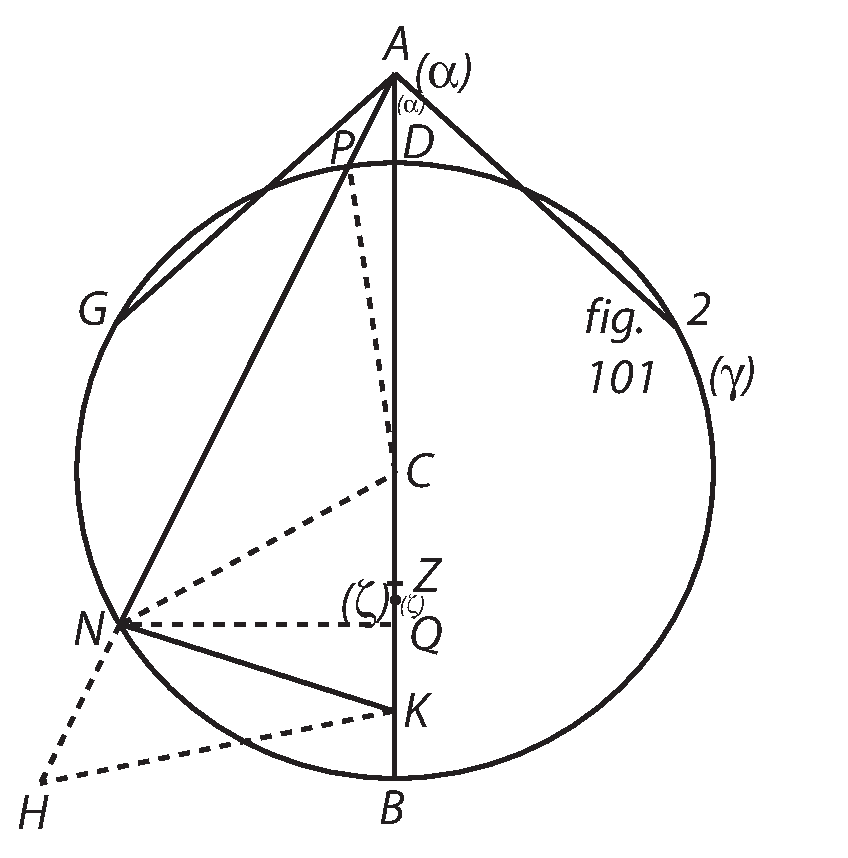
\includegraphics[width=0.4\textwidth]{images/T8_Barrow-2}
\end{center}
\clearpage


\pagenumbering{arabic}
\beginnumbering

%CH \part in \addpart geaendert, damit Ueberschrift keine Nummer
\addtocontents{toc}{\vspace{5mm}}
\addpart[\large\uppercase{I. Observata philosophica}]{\large\protect\textso{I. OBSERVATA PHILOSOPHICA}}
\clearpage{\pagestyle{empty}\cleardoublepage}            
\renewcommand*{\chapterpagestyle}{firstchapter}
\renewcommand*{\chapterheadstartvskip}{\vspace*{15.5ex}}
%\thispagestyle{firstchapter}
\chapter[\scriptsize\uppercase{Observata Philosophica in itinere Anglicano 1673}]{\uppercase{Observata philosophica in itinere Anglicano sub initium anni 1673}\newline\lbrack M\"arz 1673\rbrack}%
  \addcontentsline{toc}{chapter}{\hspace{5.5pt}\thechapter\enskip Observata philosophica in itinere Anglicano sub initium anni 1673\\\protect\rule[0cm]{2pt}{0pt}\lbrack M\"arz 1673\rbrack}%
  % \addcontentsline{toc}{chapter}{\hspace{5.5pt}\thechapter\enskip Observata philosophica in itinere Anglicano sub initium anni 1673%
% \newline\protect\rule[0mm]{2pt}{0pt}
\markleft{\scriptsize\uppercase{I. Observata philosophica}}
  \vspace{8mm}        	 
       
        
        \begin{ledgroupsized}[r]{120mm}
        \footnotesize 
        \pstart        
        \noindent\textbf{\"{U}berlieferung:}  
        \pend
        \end{ledgroupsized}
      
       
              \begin{ledgroupsized}[r]{114mm}
              \footnotesize 
              \pstart \parindent -6mm
              \makebox[6mm][l]{\textit{L}}Konzept: LH IV 8, 22 Bl. 72 \textendash 73. 1 Bog. 4\textsuperscript{o}. Insgesamt ca. 2 S. Textfolge 72 r\textsuperscript{o}, 73 v\textsuperscript{o}, 72 v\textsuperscript{o}, 73 r\textsuperscript{o}. Nach dem Beschreiben hat wahrscheinlich zu Transportzwecken eine weitere Faltung des Bogens stattgefunden, wodurch die untere H\"{a}lfte des Bl. 72 r\textsuperscript{o} zur Außenseite wurde, wie F\"{a}rbung und Abrieb zeigen. Die beiden \"{a}ußeren Seiten (72 r\textsuperscript{o}, 73 v\textsuperscript{o}) sind zweispaltig eng beschrieben. Der Text ist in Rubriken unterteilt, die mit den am Anfang aufgelisteten Wissenschafts-Bezeichnungen \"{u}berschrieben sind. Die Eintr\"{a}ge zu unterschiedlichen Rubriken wurden nachtr\"{a}glich durch Tintenstriche voneinander abgesetzt. Am oberen und rechten Rand auf Bl. 72 r\textsuperscript{o} sind mehrere Nachtr\"{a}ge zu den Rubriken auf Bl. 73 v\textsuperscript{o}. Auf den beiden inneren Seiten (72 v\textsuperscript{o}, 73 r\textsuperscript{o}) wird die Einteilung der Vorderseiten durch Spiegelung an der Papierebene exakt reproduziert, einschließlich der damit einhergehenden unregelm\"{a}ßigen Aufteilung der Seiten und der rechtsb\"{u}ndigen Auff\"{u}hrung der Bezeichnungen der Rubriken. Die R\"{u}ckseiten sind jedoch bis auf je eine Eintragung leer. Da die Einteilung nach Rubriken das Ordnungsprinzip dieser Aufzeichnungen ist, und auf Grund der sp\"{a}teren Benutzung der R\"{u}ckseiten, ergibt sich die Textfolge Bl. 72 r\textsuperscript{o}, 73 v\textsuperscript{o} mit Einf\"{u}gungen, 72 v\textsuperscript{o}, 73 r\textsuperscript{o}. Der vorliegende Text hat nicht den geplanten Umfang erreicht. Das ergibt sich aus den vorbereiteten, aber nicht ausgef\"{u}llten Rubriken auf den R\"{u}ckseiten (72 v\textsuperscript{o}, 73 r\textsuperscript{o}), und aus einem Verweis in den Chymica auf einen Eintrag in den Medica, der dort nicht ausgef\"{u}hrt worden ist.\pend
              \end{ledgroupsized}
       
              \begin{ledgroupsized}[r]{114mm}
              \footnotesize 
              \pstart \parindent -6mm
              \makebox[6mm][l]{\textit{E}}\textsc{K. I. Gerhardt}, \cite{00241}\textit{Leibniz in London}, in: \textit{Sitzungsberichte der Preußischen Akademie der Wissenschaften} X (1891) S. 157\textendash 176, darin S. 165f. (Teildruck). Englische \"{U}bersetzung in: \textsc{J. M. Child}, \cite{00242}\textit{The Early Mathematical Manuscripts of Leibniz}, Chicago 1920, S. 184\textendash 186. Nachdruck Mineola 2005.\\Cc 2, Nr. 344\pend
              \end{ledgroupsized}
        %\normalsize
        \vspace*{5mm}
        \begin{ledgroup}
        \footnotesize 
        \pstart
      \noindent\footnotesize{\textbf{Datierungsgr\"{u}nde}: Der Zeitpunkt der Anfertigung ist am Beginn des Textes zwei Mal als initium anni 1673 festgehalten. Weiterhin besteht eine auffallende Korrespondenz der Themen in einem Brief an Oldenburg vom 8. M\"{a}rz 1673 (\textit{LSB} III, 1 N. 9) zu den hier festgehaltenen Observata. Vermutlich sind Teile des vorliegenden Textes in direkter Umgebung des Briefes entstanden. Diese Datierung wird unterst\"{u}tzt durch das Wasserzeichen im Bl. 72, das eine eindeutige Konzentration auf M\"{a}rz bis Mai 1673 zeigt (vgl. \textit{LSB} VII, 3 N. 19). Jedoch ist der Text, wie an den stark variierenden Schriftbildern und einigen Wiederholungen erkennbar wird, bei unterschiedlichen Gelegenheiten geschrieben worden. Daher erfolgt die Datierung nicht genauer als M\"{a}rz 1673.}
        \pend
        \end{ledgroup}
      
        \vspace*{8mm}
        \pstart 
        \normalsize
        \centering[72 r\textsuperscript{o}] Observata Philosophica\\in itinere Anglicano\\sub initium anni 1673.\pend \vspace{1.0ex} \pstart Cum initio anni 1673. Ablegato Moguntino illustrissimo Baroni Sch\"{o}nbornio\protect\index{Namensregister}{\textso{Mainz: Johann Philipp von Sch\"{o}nborn} (Elector Moguntini), Bischof von W\"{u}rzburg u. Worms, Kurf\"{u}rst 1647\textendash 1673} Electoris Moguntini ex fratre nepoti, Parisiis\protect\index{Ortsregister}{Paris (Parisii)} Londinum\protect\index{Ortsregister}{London (Londinum)} comes ivissem, etsi vix permissa in Anglia\protect\index{Ortsregister}{England (Anglia)} mensis mora, inter varias interturbationes, operam dedi tamen philosophiae quoque incrementis cognoscendis, quando nunc ea potissimum fama gens illa floret. \pend \pstart Diarium condere taediosum et minutum, et ipsa inaequalitate, ingratum, neque enim eadem omnium dierum fortuna est, et nunc acervatur materia annotandi, nunc ingenti vacuo hiat. Quare fortasse satius fuerit, ire per capita rerum, observatione observationem velut vocante.\pend \pstart Annotandorum haec summa capita fieri possunt: Arithmetica, Geometrica, Musica\protect\index{Sachverzeichnis}{musica}, Optica, Astronomica, Mechanica, Pneumatica, Meteorologica\protect\index{Sachverzeichnis}{meteorologica}, Hydrostatica, Magnetica, Nautica, Botanica\protect\index{Sachverzeichnis}{botanica}, Anatomica\protect\index{Sachverzeichnis}{anatomica}, Chymica\protect\index{Sachverzeichnis}{chymica}, Medica\protect\index{Sachverzeichnis}{medica}, Miscellanea.\pend \pstart In \edtext{\textso{Arithmeticis}}{\lemma{\textso{Arithmeticis}}\Afootnote{\textit{doppelt unterstrichen}}} \edtext{Linea}{\lemma{\textso{Arithmeticis}}\Afootnote{ \textit{ (1) }\ notabilis est \textit{Trigonometria Britannica} fol. in qua Logarithmi\protect\index{Sachverzeichnis}{logarithmus|textit} computati sunt ad centesimam usque gradus partem, \textit{(a)}\ ad \textit{(b)}\ ac proinde pene ad minutum secundum \textit{ (2) }\ Linea \textit{ L}}} proportionum, \edtext{seu}{\lemma{}\Afootnote{seu \textit{ erg.} \textit{ L}}} Gunters\protect\index{Namensregister}{\textso{Gunter,} Edmund 1581\textendash 1626} Lini\protect\index{Sachverzeichnis}{Gunters Linea}, aliis \edtext{doublescale}{\lemma{doublescale}\Bfootnote{Vermutl. Verweis auf Gunters\protect\index{Namensregister}{\textso{Gunter,} Edmund 1581\textendash 1626|textit} Rechenst\"{a}be\protect\index{Sachverzeichnis}{Rechenstab}, vgl. \cite{00275}\textit{LSB} III, 1, S.~678f.}}. \edtext{\textit{Logarithmotechnia}}{\lemma{}\Afootnote{\textit{Logarithmotechnia} \textbar\ Mercatoris\protect\index{Namensregister}{\textso{Mercator,} Nicolaus 1620\textendash 1687} Pellii\protect\index{Namensregister}{\textso{Pell} (Pellius), John 1611\textendash 1685} terminationes numerorum quadratorum\protect\index{Sachverzeichnis}{numeri quadrati}. \textit{ gestr.}\ \textbar\ seu \textit{ L}}}
        \edtext{}{\lemma{\textit{Logarithmotechnia}}\Bfootnote{\cite{00141}\textsc{N. Mercator}, \textit{Logarithmotechnia}, London 1668. Leibniz' Kenntnis dieses Buches vermutl. durch \textsc{I. Wallis}, \cite{00236}\textit{Logarithmotechnia Nicolai Mercatoris}, \textit{PT} 3 (1668), S.~753\textendash 764. Zu dem gestrichenen Teil der Notiz \textsc{J. Pell}, \cite{00229}\textit{Tabulae}, London 1672.}} seu compendium calculandi Logarithmos\protect\index{Sachverzeichnis}{logarithmus}; dignoscere numeros quadratos\protect\index{Sachverzeichnis}{numeri quadrati} a non quadratis ex terminationibus. \pend \pstart Machina\protect\index{Sachverzeichnis}{machina!Morlandi} Morlandi\protect\index{Namensregister}{\textso{Morland,} Samuel 1625\textendash 1695}\edtext{}{\lemma{Morlandi.}\Bfootnote{Zu Leibniz' Kenntnis der Rechenmaschine Morlands\protect\index{Namensregister}{\textso{Morland,} Samuel 1625\textendash 1695|textit} vgl. \cite{00247}\textit{LSB} III, 1, S.~21, und Marginalie in \cite{00205}\textsc{S. Morland, }\textit{Arithmetick Instruments}, London 1673, vgl. dazu \cite{00217}\textit{An Accompt of some Books}, \textit{PT} 8 (1673), S.~6048f.; auch \cite{00276}\textit{LSB} III, 6, S.~330.}}.\pend \pstart \textso{Algebra}. Corpus Algebrae Anglicum \edtext{opus}{\lemma{opus}\Afootnote{ \textit{ (1) }\ 20 \textit{ (2) }\ 27 \textit{ L}}} 27 annorum. Algebra Pellii\protect\index{Namensregister}{\textso{Pell} (Pellius), John 1611\textendash 1685}\edtext{}{\lemma{Algebra}\Bfootnote{\textsc{J. H. Rahn, }\cite{00139}\textit{Algebra}, London 1668.}}. In priore, parum regularum, multum exemplorum selectorum. Renaldinus\protect\index{Namensregister}{\textso{Renaldini} (Renaldinus), Carlo 1615\textendash 1698} non aestimatur in Anglia\protect\index{Ortsregister}{England (Anglia)}.\pend \pstart \textso{Geometrica}\protect\index{Sachverzeichnis}{geometrica}. Tangentes\protect\index{Sachverzeichnis}{tangens} omnium figurarum\edtext{}{\lemma{figurarum}\Bfootnote{Vermutl. Bemerkung zu einem Brief von R. Sluse\protect\index{Namensregister}{\textso{Sluse,} Ren\'{e} Fran\c{c}ois Walter de 1622	\textendash 1685|textit} vom 17. Januar 1673 an die Royal Society; vgl. \cite{00248}\textit{LSB} III, 1, S.~32 und \cite{00154}\textit{BH} III, S. 74.}}. Figurarum geometricarum explicatio per motum puncti in moto lati.\pend \pstart Quadrantes\protect\index{Sachverzeichnis}{quadrans}\edtext{}{\lemma{Quadrantes}\Bfootnote{F\"{u}r die Quadranten und die beiden folgenden Instrumente vgl. \textsc{Th. Sprat, }\cite{00098}\textit{History}, London 1667, S.~246.}} 18 pollicum meliores omnibus hactenus usitatis, terra, pro angulis sumendis. Instrumentum sumendi angulum\protect\index{Sachverzeichnis}{instrumentum!sumendi angulum} per reflex. ita ut oculus simul videat duo obiecta, both as touching in the same point, quanquam vel semicirculo distent, magni usus in observ. marit.\protect\index{Sachverzeichnis}{observatio maritima} $\langle$Stay$\rangle$\edtext{}{\lemma{$\langle$Stay$\rangle$}\Bfootnote{In Vorlage Staff (\textsc{Th. Sprat}, \cite{00098}a.a.O., S.~246).}} pro \astrosun\ altit., wiewohl schatten auff 3 fuß distance so ist doch keine penumbra, und der schatten kan distinguirt werden ad quartam partem minuti. Niveau sive linea horizontalis sine errore 2\textsuperscript{dorum} aliquot.\edtext{}{\lemma{aliquot.}\Bfootnote{Vgl. \textsc{Th. Sprat, }\cite{00098}a.a.O., S.~248.}} (S.H)\edtext{}{\lemma{(S.H)}\Bfootnote{Abk\"{u}rzung f\"{u}r \textsc{Th. Sprat, }\cite{00098}\textit{History of the Royal Society}, London 1667.}}\pend \pstart \textso{Musica}\protect\index{Sachverzeichnis}{musica}. Character ejus universalis. Systema de \edtext{Birthinena}{\lemma{Birthinena}\Bfootnote{Vgl. dazu die Voranzeige in \textit{Another advertisement}, \cite{00278}\textit{PT} 7 (1672), S.~5153f. eines Buches \textsc{J. Birchensha}\protect\index{Namensregister}{\textso{Birchensha,} John 1605?\textendash 1681|textit}, \textit{Syntagma Musicae}. Trotz Besuch bei der Royal Society (vgl. \cite{00154}\textit{BH} I, S.~457f.) und Voranzeige ist das Buch nicht erschienen.}}. Vossius\protect\index{Namensregister}{\textso{Vossius} (Voss.), Isaac 1618\textendash 1689} Musica edet\edtext{}{\lemma{edet.}\Bfootnote{\textsc{I. Voss, }\cite{00161}\textit{De poematum cantu}, Oxford 1673; vgl. \cite{00249}\textit{LSB} III, 1, S.~87 und \cite{00218}\textit{An Accompt of Two Books}, \textit{PT} 8 (1673), S.~6024\textendash 6030.}}.\pend \pstart \textso{Optica}\protect\index{Sachverzeichnis}{optica}. Locuti sunt mihi de phaenomeno quodam quod Barrovius\protect\index{Namensregister}{\textso{Barrow} (Barrovius), Isaac 1630\textendash 1677} fatetur se solvere non posse\edtext{}{\lemma{posse}\Bfootnote{Vgl. \cite{00250}\textit{LSB} III, 1, S. 87f. und das St\"{u}ck N. 26 in diesem Band.}}. Neutonii\protect\index{Namensregister}{\textso{Newton} (Neuton, Neutonus), Isaac 1642\textendash 1727} difficultas soluta hactenus non est\edtext{}{\lemma{est}\Bfootnote{Vermutl. Kommentar zu der anhaltenden Auseinandersetzung \"{u}ber Newtons\protect\index{Namensregister}{\textso{Newton} (Neuton, Neutonus), Isaac 1642\textendash 1727|textit} Farbenlehre, vgl. \cite{00251}\textit{LSB} III, 1, S.~44.}}. P. Pardies\protect\index{Namensregister}{\textso{Pardies,} Ignace Gaston SJ 1636\textendash 1673} manus dante\edtext{}{\lemma{dante}\Bfootnote{Zu Pardies\protect\index{Namensregister}{\textso{Pardies,} Ignace Gaston SJ 1636\textendash 1673|textit} vgl. \cite{00251}\textit{LSB} III, 1, S.~43.}}. Hookius\protect\index{Namensregister}{\textso{Hooke} (Hookius, Hook), Robert 1635\textendash 1703} \edtext{Instrumento}{\lemma{Hookius}\Afootnote{ \textit{ (1) }\ spem \textit{ (2) }\ Instrumento \textit{ L}}} Catadioptrico\protect\index{Sachverzeichnis}{instrumentum!catadioptricum}\edtext{}{\lemma{Catadioptrico}\Bfootnote{Vgl. \cite{00251}\textit{LSB} III, 1, S.~43.}} 9 pedum praestabit, quod alii 50. motus eos incommodat. Secretum aperturae maximae, quae tanta inprimis Microscopiis\protect\index{Sachverzeichnis}{microscopium} dari possit, quanta objecti distantia est. Materia speculorum\protect\index{Sachverzeichnis}{speculum}, quae aeris injuriis resistat, cujus politura \edtext{pura}{\lemma{politura}\Afootnote{ \textit{ (1) }\ pulchra \textit{ (2) }\ pura \textit{ L}}} ut vitri oleum\protect\index{Sachverzeichnis}{vitri oleum}, quo inungenda specula\protect\index{Sachverzeichnis}{speculum}, ut rubigini resistant\edtext{}{\lemma{resistant}\Bfootnote{Vgl. zu Hookes\protect\index{Namensregister}{\textso{Hooke} (Hookius, Hook), Robert 1635\textendash 1703|textit} Catadioptricum \cite{00251}\textit{LSB} III, 1, S.~43 und \cite{00154}\textit{BH} III, S. 72 und 74.}}. Cock\protect\index{Namensregister}{\textso{Cock,} Christopher} \edtext{microscopia}{\lemma{microscopia}\Bfootnote{Christopher Cock\protect\index{Namensregister}{\textso{Cock,} Christopher|textit} (Lebensdaten unbekannt) hatte mehreren Mitgliedern der Royal Society Mikroskope gebaut, darunter auch das Mikroskop, mit dem Hooke\protect\index{Namensregister}{\textso{Hooke} (Hookius, Hook), Robert 1635\textendash 1703|textit} die Beobachtungen zur Micrographia durchf\"{u}hrte.}}\protect\index{Sachverzeichnis}{microscopium}, \edtext{sabuli}{\lemma{microscopia,}\Afootnote{ \textit{ (1) }\ sabulum \textit{ (2) }\ sabuli \textit{ L}}} granum instar ovi columbini pediculus ut capra et capellus ut chorda. Schmethwick\protect\index{Namensregister}{\textso{Smethwick} (Schmethwick), Francis}\edtext{}{\lemma{Schmethwick}\Bfootnote{Die Lebens\-daten des F. Smethwick\protect\index{Namensregister}{\textso{Smethwick} (Schmethwick), Francis|textit} sind unbekannt. Er ist nachgewiesen durch einen Bericht \"{u}ber seine Vorf\"{u}hrung nicht-sph\"{a}risch geschliffener Gl\"{a}ser in einer Sitzung der Royal Society, \cite{00219}\textit{An Account of the Invention of Grinding Optick and Burning Glasses, of a figure not-Spherical, produced before the Royal Society}, \textit{PT} 3 (1668), S.~631\textendash 632.}} sectionis Conicae\protect\index{Sachverzeichnis}{sectio conica} vitrum \edtext{fodert vor ein perspectiv 10 \Pfund\ sterlings}{\lemma{}\Afootnote{fodert vor ein perspectiv 10 \Pfund\ sterlings \textit{ erg.} \textit{ L}}}; non sunt tanti, putat ipse esse hyperbolam\edtext{}{\lemma{hyperbolam}\Bfootnote{Zu misslungenen Versuchen, hyperbolische Linsen herzustellen, vgl. \textit{An account of two books. I. Renati Franc. Slusii Mesolabum}, \cite{00284}\textit{PT} 4 (1669), S.~903\textendash 912, bes. S.~904 und \textit{An answer written to the publisher}, \cite{00285}\textit{PT} 8 (1673), S.~6112.}}. Cock\protect\index{Namensregister}{\textso{Cock,} Christopher} nunc \edtext{telescopium\protect\index{Sachverzeichnis}{telescopium}}{\lemma{telescopium}\Bfootnote{Die Royal Society beauftragte Cock\protect\index{Namensregister}{\textso{Cock,} Christopher|textit}, ein Teleskop nach dem Konzept Newtons\protect\index{Namensregister}{\textso{Newton} (Neuton, Neutonus), Isaac 1642\textendash 1727|textit} zu bauen, vgl. \cite{00154}\textit{BH} III, S.~19, 43, 49 und 57.}} 50 pedum Drebelii\protect\index{Namensregister}{\textso{Drebbel} (Drebelius, Drebel), Cornelius 1572\textendash 1633} \edlabel{telescopstart}Telescop.\pend \pstart \edtext{vergroßern\edlabel{telescopend}}{{\xxref{telescopstart}{telescopend}}\lemma{Telescop.}\Afootnote{ \textit{ (1) }\ Unter \textit{ (2) }\ vergroßernbrillen \textit{ L}}}brillen \pend \pstart Flexible Gl\"{a}ser mit $\langle$−$\rangle$ Selenitis. U)\edtext{}{\lemma{U)}\Bfootnote{Vermutl. K\"{u}rzel f\"{u}r \textsc{R. Boyle,} \cite{00155}\textit{Usefulness}, London 1663.}} ohne Glaser foliiren und also Spigl\protect\index{Sachverzeichnis}{Spiegel} draus machen, desideratum.\pend%Stork ok    
    \pstart [73 v\textsuperscript{o}] \textso{Astronomica}. Hookii\protect\index{Namensregister}{\textso{Hooke} (Hookius, Hook), Robert 1635\textendash 1703} designatio observandi, Tellus\protect\index{Sachverzeichnis}{tellus} ne aliquando sensibiliter accederet \edtext{abscederetque fixis}{\lemma{accederet}\Afootnote{ \textit{ (1) }\ astris fixis\protect\index{Sachverzeichnis}{stella!fixa|textit} \textit{ (2) }\ abscederetque fixis \textit{ L}}}, unde probaretur, eam non esse in centro Mundi eum in finem tubum perpendiculariter erexit, et stellas observavit, quae sunt verticales. Ipse dorso supinus incumbens exactissime magnitudines observabat. Theoria planetarum\protect\index{Sachverzeichnis}{theoria planetarum}, Ludimagistri cujusdam Londinensis, eaque non inepta. Praedictiones tempestatum\protect\index{Sachverzeichnis}{praedictio tempestatum} ex coelo, cum ipsis plagis ventorum, Londinum, urbs observationibus inepta\edtext{}{\lemma{inepta}\Bfootnote{Zu Wetterbeobachtungen durch Leibniz vgl. N. 37, \cite{00251}\textit{LSB} III, 1, S.~41 und durch die Royal Society \cite{00154}\textit{BH} III, S.~75.}}. Praedictio cometarum\protect\index{Sachverzeichnis}{praedictio cometarum}. Hevelii\protect\index{Namensregister}{\textso{Hevelius,} Johannes 1611\textendash 1687}\edtext{}{\lemma{cometarum}\Bfootnote{Vgl. \cite{00215}\textit{The motion of the late Comet praedicted}, \textit{PT} 1 (1665), S.~3\textendash 8, einen Bericht \"{u}ber eine Sendung des A. Auzout\protect\index{Namensregister}{\textso{Auzout} (Auzutus), Adrien 1622\textendash 1603|textit} mit der ersten Beschreibung einer Kometenbahn. Wegen des nachfolgenden Hinweises vielleicht auch \textsc{J. Hevelius, }\cite{00152}\textit{Prodromus Cometicus}, Danzig 1665, und auch \cite{00220}\textit{Extract of a Letter of M. Hevelius}, \textit{PT} 7 (1672), S.~4017f.}} organica coelestis\edtext{}{\lemma{coelestis}\Bfootnote{\textsc{J. Hevelius, }\cite{00151}\textit{Machina coelestis}, Danzig 1673.}}. Instrumentum 2\textsuperscript{da} minuta temporis inveniendi sole. S.H)\edtext{}{\lemma{sole.}\Bfootnote{Vgl. \textsc{Th. Sprat, }\cite{00098}a.a.O., S.~246.}} add. Geometr. Lunae mappa\protect\index{Sachverzeichnis}{mappa lunae} in relievo\edtext{}{\lemma{relievo}\Bfootnote{Vgl. \textsc{Th. Sprat, }\cite{00098}a.a.O., S.~315.}}.\pend \pstart \textso{Mechanica }\protect\index{Sachverzeichnis}{mechanica} Hook\protect\index{Namensregister}{\textso{Hooke} (Hookius, Hook), Robert 1635\textendash 1703} de aequiresistentibus \edtext{figuris\protect\index{Sachverzeichnis}{figurae aequiresistentes}}{\lemma{figuris}\Bfootnote{Vgl. dazu \cite{00251}\textit{LSB} III, 1, S.~41f.}} demonstratio. Horologium annuum\protect\index{Sachverzeichnis}{horologium!annuum} et ultra. Motus perennis\label{DrebInst} Drebelii\protect\index{Namensregister}{\textso{Drebbel} (Drebelius, Drebel), Cornelius 1572\textendash 1633} sub Jacobo\protect\index{Namensregister}{\textso{England: Jakob I.} (Rex Jacobus, R. Jac.), K\"{o}nig von England 1603\textendash 1625}\edtext{}{\lemma{Jacobo}\Bfootnote{C. Drebbel hatte zwischen 1606 und 1609 f\"{u}r James I.\protect\index{Namensregister}{\textso{England: Jakob I.} (Rex Jacobus, R. Jac.), K\"{o}nig von England 1603\textendash 1625} eine astronomische Uhr konstruiert (beschrieben durch \textsc{Th. Tymme, }\cite{00162}\textit{Dialogue}, London 1612, S.~60\textendash 63), die durch steigendes oder fallendes Wasser in einer Glaskugel auch die Gezeiten anzeigte. Die Beschreibung hebt die perpetual motion der Uhr hervor.}}. Horologium pendulum\protect\index{Sachverzeichnis}{horologium!pendulum} conveniens Soli.\pend 
\pstart Experimenta de gradibus resistentiae\protect\index{Sachverzeichnis}{resistentia!lignorum} et flexibilitatis\protect\index{Sachverzeichnis}{flexibilitas lignorum} summae, variorum lignorum\edtext{}{\lemma{lignorum}\Bfootnote{Vgl. \textsc{Th. Sprat, }\cite{00098}a.a.O., S.~227.}}. S.H) De ligno\footnote{\textit{Oberhalb} de ligno quod semestri: Locust Tree, arcus} quod semestri tensione nihil virium amittit\edtext{}{\lemma{amittit}\Bfootnote{Vgl. \textsc{Th. Sprat, }\cite{00098}a.a.O., S.~198.}} S.H)\pend 
\pstart $\langle$\edtext{Movet}{\lemma{Movet}\Afootnote{\textit{Lesung unsicher}}}$\rangle$ $\langle$−$\rangle$ wie eine kammer. M. Coterel\protect\index{Namensregister}{\textso{Coterel}}, pendulum sine sono, et quod noctu igne monstrat horam, luce quadam tenui, dixit M. Coterel\protect\index{Namensregister}{\textso{Coterel}}. De recipiendis et praeservandis viribus pulveris pyrii\protect\index{Sachverzeichnis}{pulvis!pyrius}\edtext{}{\lemma{viribus}\Bfootnote{Vgl. \textsc{Th. Sprat, }\cite{00098}a.a.O., S.~250.}} S.H) Drebels\protect\index{Namensregister}{\textso{Drebbel} (Drebelius, Drebel), Cornelius 1572\textendash 1633} m. p. se restituens\edtext{}{\lemma{restituens}\Bfootnote{Das Buch \textsc{Th. Tymme,} \cite{00162}a.a.O., verspricht im Titel eine \textit{Artificiall perpetuall motion}. Drebbels Konstruktion wird jedoch nicht als perpetuum mobile pr\"{a}sentiert, sondern als Antrieb wird ein \textit{fierie spirit out of the minerall matter, ioyn[ed] with his proper Aire} genannt. (vgl. \textsc{Th. Tymme}, \cite{00162}a.a.O., S.~60\textendash 63). Die wiederholte Notiz Leibniz' zu diesem Gegenstand stimmt mit seinem anhaltenden Interesse an einem motus perennis \"{u}berein.}}; corruptus a R. Jac.\protect\index{Namensregister}{\textso{England: Jakob I.} (Rex Jacobus, R. Jac.), K\"{o}nig von England 1603\textendash 1625} ipso absente. Ein Franzoß unseres Chevalier zu francfort hat etwas, so wie ein Bliz\protect\index{Sachverzeichnis}{Blitz} schrecken soll dixit \edtext{Sch\protect\index{Namensregister}{\textso{Schroeter} (Schr., Sch.), Wilhelm 1644\textendash 1688}}{\lemma{Sch.}\Bfootnote{Die mit Sch. bezeichnete Person oder Quelle ist nicht eindeutig gekl\"{a}rt. Ein Gro{\ss}teil der so gekennzeichneten Nachrichten ist in Deutsch festgehalten und enth\"{a}lt mehrfach Informationen zu Ereignissen in Deutschland. Zudem lautet die Abk\"{u}rzung ein Mal Schr. Daher wird mit dem K\"{u}rzel Sch. vermutlich Schroeter\protect\index{Namensregister}{\textso{Schroeter} (Schr., Sch.), Wilhelm 1644\textendash 1688|textit} bezeichnet. Diese Annahme wird durch mehrere Erw\"{a}hnungen Schroeters in Leibniz' Briefen (\cite{00252}\textit{LSB} III, 1, S.~38 und 48), die anf\"{a}nglich auch Austausch mit Schroeter nahelegen, unterst\"{u}tzt.}}.\pend \pstart \textso{Pneumatica }\protect\index{Sachverzeichnis}{pneumatica} Boylii\protect\index{Namensregister}{\textso{Boyle} (Boylius, Boyl., Boyl), Robert 1627\textendash 1691} experimenta de relatione aeris et flammae\protect\index{Sachverzeichnis}{flamma}\edtext{}{\lemma{flammae}\Bfootnote{\textsc{R. Boyle}, \textit{New experiments, touching the relations betwixt flame and air} vermutl. von Leibniz gelesen als Teil der \cite{00156}\textit{Tracts}, London 1672 (\cite{00017}\textit{BW} 7, S.~73\textendash 131). Zu diesem Buch vgl. S.~\pageref{tracts}.}}. Steph. ab Angelis\protect\index{Namensregister}{\textso{Angeli,} Stefano degli 1623\textendash 1697} del peso dell' aria\edtext{}{\lemma{aria}\Bfootnote{\textsc{St. degli Angeli, }\cite{00165}\textit{Gravit\`{a}}, Padua 1672.}}.\pend \pstart \textso{Meteorologica}\protect\index{Sachverzeichnis}{meteorologica}: Bohun\protect\index{Namensregister}{\textso{Bohun,} Ralph 1639\textendash 1716} de ventis observationes Nautarum\edtext{}{\lemma{Nautarum}\Bfootnote{\textsc{R. Bohun, }\cite{00166}\textit{Dis\-course}, Oxford 1671.}}; \edtext{Wetter Glock\protect\index{Sachverzeichnis}{Wetterglocke}}{\lemma{Wetter Glock}\Bfootnote{Vgl. \textsc{Th. Sprat, }\cite{00098}a.a.O., S.~313.}} Wrennii\protect\index{Namensregister}{\textso{Wren} (Wrennius), Christopher 1632\textendash 1723} et Hookii\protect\index{Namensregister}{\textso{Hooke} (Hookius, Hook), Robert 1635\textendash 1703} Wallisius\protect\index{Namensregister}{\textso{Wallis} (Wallisius), John 1616\textendash 1703} observat.\pend \pstart Stellarum cadentium\protect\index{Sachverzeichnis}{stella!cadentia} examinatio: materia mucilaginosa dicta staar-shoot\edtext{}{\lemma{staar\textendash shoot}\Bfootnote{Vgl. \textsc{Th. Sprat, }\cite{00098}a.a.O., S.~227.}} S.H).\pend 
\pstart \textso{Hydrostatica }\protect\index{Sachverzeichnis}{hydrostatica} \edtext{navis}{\lemma{navis}\Bfootnote{Drebbel hatte zwischen 1620\textendash 1624 unter James I.\protect\index{Namensregister}{\textso{England: Jakob I.} (Rex Jacobus, R. Jac.), K\"{o}nig von England 1603\textendash 1625} mehrere Ruderboote durch Lederüberzug und Schnorchel zu Unterwasserfahrzeugen ver\"{a}ndert und durch die Themse fahren lassen. Dazu ein Bericht bei Boyle 1662.}} Drebelii\protect\index{Namensregister}{\textso{Drebbel} (Drebelius, Drebel), Cornelius 1572\textendash 1633}, \edtext{ejus}{\lemma{Drebelii,}\Afootnote{ \textit{ (1) }\ remi \textit{ (2) }\ ejus \textit{ L}}} mirabiles\edtext{}{\lemma{mirabiles}\Bfootnote{Vgl. dazu \cite{00253}\textit{LSB} II, 1, S.~263.}}, ideo sub Carolo\protect\index{Namensregister}{\textso{England: Karl I.} (Carolus), K\"{o}nig von England und Schottland 1625\textendash 1649}\protect\index{Namensregister}{\textso{England: Karl II.} (Carolus), K\"{o}nig von England 1649\textendash 1685}.\pend \pstart  Boylius\protect\index{Namensregister}{\textso{Boyle} (Boylius, Boyl., Boyl), Robert 1627\textendash 1691} quaedam Hydrostatica \edtext{publicabit}{\lemma{publicabit}\Bfootnote{Nach M\"{a}rz 1673 ist ein Titel Boyles mit dem Stichwort Hydrostatica nicht bekannt (vgl. \cite{00017}\textit{BW} 7, S.~335f.; 11, S.~189\textendash 196). Entweder kannte Leibniz ein nicht realisiertes Projekt Boyles, oder er bekam Zugang zu Boyles \textit{Hydrostatical Discourse} und \textit{Hydrostatical Letter} in den \cite{00156}\textit{Tracts} (\cite{00017}\textit{BW} 7, S.~73\textendash 184) erst zu einem sp\"{a}teren Zeitpunkt. Daf\"{u}r spricht das Exzerpt dieser Publikation als Nachtrag, vgl. S.~\pageref{tracts}. Vgl. auch \cite{00216}\textit{An Accompt of two Books}, \textit{PT} 8 (1673), S.~5197\textendash 6006.}}. Dusonius\protect\index{Namensregister}{\textso{Du Sonius} (Dusonius), Aigmont 1604\textendash ?} nunc in fodinarum aquis amoliendis exercetur.\pend 
\pstart (S.H de figuris corporum, ita accommodandis, ut per diversa media simul fundum attingant. \textso{Experim}. machina 1000 tonnen waßer in einer stunde aus\-zupumpen. (an modo momentum.) dixit Sch. Modulum esse in Soc. Repositorium. Einer der mit einem inst. so eine cheminee aus dem waßer raus gehend hat, etliche stunden kan unter waßer seyn. Relatio de \edtext{Cingulo aere pleno, quo}{\lemma{de}\Afootnote{ \textit{ (1) }\ homine qu \textit{ (2) }\ Cingulo aere pleno, quo \textit{ L}}} in aqua iri potest (coram duce Florentiae\protect\index{Ortsregister}{Florenz (Fiorenze, Florentia)}) S.H) adde Christianum IV.\protect\index{Namensregister}{\textso{D\"{a}nemark:} Christian IV., K\"{o}nig von D\"{a}nemark 1588\textendash 1648} Daniae\protect\index{Ortsregister}{Danemark@D\"{a}nemark (Dania)}.
\pend\newpage
\pstart \textso{Nautica}. Experimenta Brunckeri\protect\index{Namensregister}{\textso{Brouncker} (Brunckerus), William Viscount 1620\textendash 1684}, apparatus ejus, canal artificiel cum tot navium formis periit me praesente. Trinity-house\protect\index{Sachverzeichnis}{Trinity\textendash house} [at]\edtext{}{\Afootnote{a\textit{\ L \"{a}ndert Hrsg.}}} London\protect\index{Ortsregister}{London (Londinum)}, ibi relationes nautarum omnes. Societas licentiam sperat percurrendi. Aqua marina dulcis. Dictionarium Nauticum. $\langle$At$\rangle$las Anglicanus. Mensura terrae\protect\index{Sachverzeichnis}{mensura terrae} vera.\pend 
\pstart \textso{Magnetica}\protect\index{Sachverzeichnis}{magnetica}. Observationes Dantiscanae, item in Hudsonsbay\edtext{}{\lemma{Hudsonsbay}\Bfootnote{Vgl. \cite{00251}\textit{LSB} III, 1, S.~43.}}. Collectanea Boylii\protect\index{Namensregister}{\textso{Boyle} (Boylius, Boyl., Boyl), Robert 1627\textendash 1691}. Ejus modus mutandi polum magnetis\protect\index{Sachverzeichnis}{polus!magnetis}. Ejus modus, acus\protect\index{Sachverzeichnis}{acus!magnetica} praeservandi. Bond\protect\index{Namensregister}{\textso{Bond,} Henry 1600?\textendash 1678}.\pend \pstart Diversio virium attractivarum\protect\index{Sachverzeichnis}{vis attractiva} interposito ferro\protect\index{Sachverzeichnis}{ferrum}. NB. Kircher\protect\index{Namensregister}{\textso{Kircher} (Kircherus), Athanasius SJ 1602\textendash 1680} de p. m.\edtext{}{\lemma{de p. m.}\Bfootnote{\textsc{A. Kircher}, \cite{00067}\textit{Magnes}, Rom 1654, S.~239\textendash 245.}} si qui divertere possit. \edtext{tum}{\lemma{possit.}\Afootnote{ \textit{ (1) }\ probatio \textit{ (2) }\ tum \textit{ L}}} per pulverem chalybeum\protect\index{Sachverzeichnis}{pulvis!chalybeus}, tum per acus\protect\index{Sachverzeichnis}{acus}, manifestare. Lineas directionis magneticae, contrarias theoriae Cartesii\protect\index{Namensregister}{\textso{Descartes} (Cartesius, des Cartes, Cartes.), Ren\'{e} 1596\textendash 1650} (Wren\protect\index{Namensregister}{\textso{Wren} (Wrennius), Christopher 1632\textendash 1723}) detegere easdem lineas in composita variorum magnetum influentia\edtext{}{\lemma{influentia}\Bfootnote{Vgl. \textsc{Th. Sprat, }\cite{00098}a.a.O., S.~221f.}}. S.H \pend 
\pstart \edtext{Magnetica\protect\index{Sachverzeichnis}{magnetica!terrella} terrella in assere plano, semiextans polis incumbens horizonti, asser respersus armatura at furrows, that flud like a sorte of helix quasi exiens ex uno polo et ad alium rediens, planum totum figuratum quasi circulis \edtext{hemisphaerii}{\lemma{hemisphaerii}\Bfootnote{Zu diesem Experiment vgl. \textsc{Th. Sprat, }\cite{00098}a.a.O., S.~315f.}}. Boylii\protect\index{Namensregister}{\textso{Boyle} (Boylius, Boyl., Boyl), Robert 1627\textendash 1691} experimenta Magnetico-chymica\edtext{}{\lemma{Magnetico-chymica}\Bfootnote{Vermutl. \textsc{R. Boyle, }\cite{00167}\textit{Specimen unum}, London 1661.}}. Bond\protect\index{Namensregister}{\textso{Bond,} Henry 1600?\textendash 1678} laßet uberal observirn trifft ziemblich zu. Boyl.\protect\index{Namensregister}{\textso{Boyle} (Boylius, Boyl., Boyl), Robert 1627\textendash 1691} se habere rationes cur desperet rem unquam regulari posse. Nautae diversi retulere Boylio\protect\index{Namensregister}{\textso{Boyle} (Boylius, Boyl., Boyl), Robert 1627\textendash 1691} summam declinationem australem\protect\index{Sachverzeichnis}{declinatio!Australis} et summam Borealem\protect\index{Sachverzeichnis}{declinatio!Borealis} fere   congruere. Boyl.\protect\index{Namensregister}{\textso{Boyle} (Boylius, Boyl., Boyl), Robert 1627\textendash 1691} hat ein groß recueil observationum de declinatione. Hudsonsbay\protect\index{Ortsregister}{Hudsonbay (Hudsonsbay)} fahrer experti daß die Nadel 25 bis 30 grad declinirt.}{\lemma{}\Afootnote{magnetica terrella [...] horizonti, asser \textit{ (1) }\ planus \textit{ (2) }\ respersus armatura [...] grad declinirt. \textit{ erg.} \textit{ L}}}\pend 
\pstart \textso{Physica}. \edtext{Boyl.\protect\index{Namensregister}{\textso{Boyle} (Boylius, Boyl., Boyl), Robert 1627\textendash 1691} diamant\protect\index{Sachverzeichnis}{Diamant} so bisweilen schwarz wird intus.}{\lemma{}\Afootnote{Boyl. diamant [...] wird intus. \textit{ erg.} \textit{ L}}} Boyl.\protect\index{Namensregister}{\textso{Boyle} (Boylius, Boyl., Boyl), Robert 1627\textendash 1691} de \edtext{Gemmis}{\lemma{Gemmis}\Bfootnote{\textsc{R. Boyle}, \cite{00240}\textit{Gems}, London 1672 (\cite{00017}\textit{BW} 7, S.~3\textendash 72), oder die lateinische Fassung \cite{00168}\textit{Exercitatio de origine gemmarum}, London 1673.}}. Boyl.\protect\index{Namensregister}{\textso{Boyle} (Boylius, Boyl., Boyl), Robert 1627\textendash 1691} mox de effluviis. Power. Glisson\protect\index{Namensregister}{\textso{Glisson,} Francis 1597\textendash 1677} de vita naturae\edtext{}{\lemma{naturae}\Bfootnote{\textsc{F. Glisson, }\cite{00170}\textit{Tractatus}, London 1672.}}. \edtext{Micrographiae   supplementa.}{\lemma{naturae.}\Afootnote{ \textit{ (1) }\ Relatio de ignivor \textit{ (2) }\ Micrographiae   supplementa. \textit{ L}}}\pend \pstart   Instr. mesurandi corporis descensus et motus ad duas tertias temporis\edtext{}{\lemma{temporis}\Bfootnote{Vgl. \textsc{Th. Sprat, }\cite{00098}a.a.O., S.~225 und 248.}}. Ignivorus in manu lavans plumbo fuso $\langle$−$\rangle$ liquida, carbones devorans ignitos, liquor Drebels\protect\index{Namensregister}{\textso{Drebbel} (Drebelius, Drebel), Cornelius 1572\textendash 1633}, so warhafftig Ebbe und flut zeigte\edtext{}{\lemma{zeigte}\Bfootnote{Zu Drebbels Instrument vgl. S.~\pageref{DrebInst}.}}.\pend \pstart \textso{Botanica }\protect\index{Sachverzeichnis}{botanica} Grey\protect\index{Namensregister}{\textso{Grew,} Nehemiah 1641\textendash 1712} \textit{Anatome}\edtext{}{\lemma{\textit{Anatome}}\Bfootnote{Kurz vor der Teilnahme Leibniz' an einigen Sitzungen der Royal Society hatte diese ihren Auftrag an N. Grew\protect\index{Namensregister}{\textso{Grew,} Nehemiah 1641\textendash 1712}, eine Anatomie der Pflanzen zu schreiben, best\"{a}tigt (vgl. \cite{00154}\textit{BH} III, S.~69), aus der Grew\protect\index{Namensregister}{\textso{Grew,} Nehemiah 1641\textendash 1712} Ausz\"{u}ge vortrug (vgl. \cite{00154}\textit{BH} III, S.~72). Anatome ist eine Referenz auf \textsc{N. Grew}, \cite{00171}\textit{An Idea of a Phytological History}, London 1673 oder Vorgriff auf \textsc{N. Grew, }\cite{00172}\textit{The Anatomy of Plants}, London 1682.}}, Malpighii\protect\index{Namensregister}{\textso{Malpighi} (Malpighius), Marcello 1628\textendash 1694} anatome\edtext{}{\lemma{anatome}\Bfootnote{Malpighii anatome bezieht sich entweder auf die fr\"{u}heren anatomischen Arbeiten des Malpighius oder Leibniz hatte wie bei Grew\protect\index{Namensregister}{\textso{Grew,} Nehemiah 1641\textendash 1712} Einsicht in Vorarbeiten zu \cite{00200}\textsc{M. Malpighi,} \textit{Anatome Plantarum}, London 1675.}} sucus duplex\protect\index{Sachverzeichnis}{sucus duplex} alter aqueus alter lacteus: et hic incongelabilis. \edtext{Morison}{\lemma{incongelabilis.}\Afootnote{ \textit{ (1) }\ Hartlieb\protect\index{Namensregister}{\textso{Hartlib} (Hartlieb), Samuel 1600\textendash 1662|textit} resp. apum Butler\protect\index{Namensregister}{\textso{Butler,} Charles 1560?\textendash 1647|textit} Monarchia foeminina \textit{ (2) }\ Morison \textit{ L}}} plantarum series\edtext{}{\lemma{series}\Bfootnote{\textsc{R. Morison, }\cite{00175}\textit{Plantarum Distributio}, Oxford 1672.}} Rey\protect\index{Namensregister}{\textso{Ray} (Rey), John 1627\textendash 1705} Itinerarium Botanicum\edtext{}{\lemma{Botanicum}\Bfootnote{Titelangabe nicht eindeutig, entweder \textsc{J. Ray, }\cite{00208}\textit{Observations made in a journey}, London 1673, oder \cite{00207}\textsc{J. Ray, }\textit{Catalogus plantarum Angliae}, London 1670.}}. Agricult. et pomicult. secretum verwant Herr Boyle\protect\index{Namensregister}{\textso{Boyle} (Boylius, Boyl., Boyl), Robert 1627\textendash 1691}.  \pend \pstart Reunio corticis arborum separati\edtext{}{\lemma{separati}\Bfootnote{Vgl. \textsc{Th. Sprat, }\cite{00098}a.a.O., S.~223.}}. S.H) De gramine (exotico) funibus fortissimis aptiore, quam cannabis\protect\index{Sachverzeichnis}{Cannabis sativa}\edtext{}{\lemma{cannabis}\Bfootnote{Vgl. \textsc{Th. Sprat, }\cite{00098}a.a.O., S.~197.}} S.H) De planta quadam mire propagativa pene ineradicabili S.H) Pfeffer\protect\index{Sachverzeichnis}{Pfeffer} aus jamaica\protect\index{Ortsregister}{Jamaika (Jamaica)} so recht wie \edtext{n\"{a}gelchen}{\lemma{n\"{a}gelchen}\Bfootnote{Vgl. \textsc{R. Boyle, }\cite{00155}\textit{Usefulness}, Teil I, S.~12 (\cite{00017}\textit{BW} 3, S.~206f.).}}. U.) Napellus sine veneno in Polonia Annus 2\textsuperscript{dus} Med. Germ.)\edtext{}{\lemma{Germ.)}\Bfootnote{\textsc{M. B. v. Berniz,} \textit{Napellus in Polonia non venenosus}. \cite{00279}\textit{Miscellanea curiosa} 2 (1671), S.~79\textendash 82.}}\pend
\pstart \textso{Anatomica }\protect\index{Sachverzeichnis}{anatomica} Willughby\protect\index{Namensregister}{\textso{Willughby,} Francis 1635\textendash 1672} itinerarium Zoicum\edtext{}{\lemma{Zoicum}\Bfootnote{\textsc{F. Willughby, }\cite{00176}\textit{Voyage through Spain}, London 1673.}}. Malphighii\protect\index{Namensregister}{\textso{Malpighi} (Malpighius), Marcello 1628\textendash 1694} \textit{De Bombyce}\edtext{}{\lemma{\textit{Bombyce}}\Bfootnote{\textsc{M. Malpighi, }\cite{00177}\textit{De bombyce}, London 1669.}}. De pullo in ovo\edtext{}{\lemma{ovo}\Bfootnote{W\"{a}hrend der Sitzung der Royal Society am 22. Januar 1673 wurde ein Brief Malpighis \"{u}ber Beobachtungen an Eiern verlesen, vgl. \cite{00154}\textit{BH} III, S.~73. Vgl. auch \textsc{R. Boyle,} \cite{00155}\textit{Usefulness}, Teil I, S.~54f. (\cite{00017}\textit{BW} 3, S.~236).}}. Butler\protect\index{Namensregister}{\textso{Butler,} Charles 1560?\textendash 1647} de apibus\edtext{}{\lemma{apibus}\Bfootnote{Vgl. \textsc{Ch. Butler, }\cite{00174}\textit{Monarchia Foeminina}, London 1673, Widmungsgedicht.}}. Schwammerdam\protect\index{Namensregister}{\textso{Swammerdam} (Schwammerdam), Jan 1637\textendash 1680} conditura uteri\protect\index{Sachverzeichnis}{uterus}\edtext{}{\lemma{conditura}\Bfootnote{\textsc{J. Swammerdam,} \cite{00201}\textit{Miraculum naturae sive uteri muliebris fabrica}, Leiden 1672. Vgl. auch \cite{00154}\textit{BH} III, S.~52.}}. Ejusdem restitutio hepatis\protect\index{Sachverzeichnis}{hepar}\edtext{}{\lemma{restitutio}\Bfootnote{Kurz vor Leibniz' Teilnahme hatte Swammerdam der Royal Society mehrere anatomische Pr\"{a}parate geschenkt, darunter einen uterus humanus und eine Arteria Hepatica, vgl. \cite{00154}\textit{BH} III, S.~71 und 76.}}. Willis\protect\index{Namensregister}{\textso{Willis,} Thomas 1621\textendash 1675} de anima brutorum seu sensitiva\edtext{}{\lemma{sensitiva}\Bfootnote{\textsc{Th. Willis, }\cite{00178}\textit{De Anima}, Amsterdam 1672.}}. \edtext{Biceps}{\lemma{sensitiva.}\Afootnote{ \textit{ (1) }\ Ejusdem de passione hyst \textit{ (2) }\ Biceps \textit{ L}}} Gallus Indicus\protect\index{Sachverzeichnis}{Gallus Indicus} in spiritu vini\protect\index{Sachverzeichnis}{spiritus!vini} conservatus. Formatio loquelae.\pend \pstart Musculi artificiales\protect\index{Sachverzeichnis}{musculi artificiales} tenduntur Elaterio pyrio pulvere\protect\index{Sachverzeichnis}{pulvis!pyrii}\edtext{}{\lemma{Musculi}\Bfootnote{Vgl. \textsc{Th. Sprat, }\cite{00098}a.a.O., S.~226.}} S.H) Caro reducta menstruo in liquorem sanguini similem\edtext{}{\lemma{similem}\Bfootnote{Vgl. \textsc{Th. Sprat, }\cite{00098}a.a.O., S.~226, und \textsc{R. Boyle,} \cite{00155}\textit{Usefulness}, Teil II, S.~20 (\cite{00017}\textit{BW} 3, S.~306).}}. S.H) Dentes lupi marini esse id quod pro Krotenstein\protect\index{Sachverzeichnis}{Kr\"{o}tnstein} venditatur, et annulis includitur\edtext{}{\lemma{includitur}\Bfootnote{Vgl. \textsc{Th. Sprat, }\cite{00098}a.a.O., S.~242.}}. S.H) Liming of the ground vermehrt der Schaff\protect\index{Sachverzeichnis}{Schaf} fettigkeit, verderbt die wolle\protect\index{Sachverzeichnis}{Wolle}\edtext{}{\lemma{wolle}\Bfootnote{Vgl. \textsc{Th. Sprat, }\cite{00098}a.a.O., S.~242.}}. Tarantulae fabulosae Transact.\edtext{}{\lemma{Transact.}\Bfootnote{Vgl. \textit{An Account of some books}, \cite{00273}\textit{PT} 3 (1668), S.~660\textendash 604 [664], darin Rezension zu I. W. Sangwerdius PD, \cite{00281}\textit{De Tarantula}, Leiden 1668.}} \edtext{Schwammerdam\protect\index{Namensregister}{\textso{Swammerdam} (Schwammerdam), Jan 1637\textendash 1680} tract. de Sanguificatione\protect\index{Sachverzeichnis}{sanguificatio}\edtext{}{\lemma{Sanguificatione}\Bfootnote{Vermutl. Referenz auf \textit{Extracts of two Letters of Dr. Swammerdam}, \cite{00224}\textit{PT} 8 (1673), S.~6040\textendash 6042, hier S.~6041.}} reddet hepati\protect\index{Sachverzeichnis}{hepar} officium promittens sibi applausum tanto majorem, quia nemo ostenderit chylum\protect\index{Sachverzeichnis}{chylus} vehi ad vasa lactea\protect\index{Sachverzeichnis}{vasa lactea} primi generis ut vocat. Quod faciat eum credere, nihil esse in illis nisi lympham albam\protect\index{Sachverzeichnis}{lympha alba} in venis lactenis apparentem, et exeuntem glandulis\protect\index{Sachverzeichnis}{glandula} intestinarum.}{\lemma{}\Afootnote{Schwammerdam\protect\index{Namensregister}{\textso{Swammerdam} (Schwammerdam), Jan 1637\textendash 1680} [...] intestinarum. \textit{ erg.} \textit{ L}}} Infans sine cerebro annus 2\textsuperscript{dus} Med. Germ.\edtext{}{\lemma{Germ.}\Bfootnote{\textsc{J. J. Wepfer,} \textit{De puella sine cerebro nata, historia}, \cite{00280}\textit{Miscellanea curiosa} 3 (1672), S.~205\textendash 208.}} 
\pend
\newpage
\pstart   \textso{Chym}\protect\index{Sachverzeichnis}{chymica}. Catal. commutandorum Lampadographia experimentalis Haakii\protect\index{Namensregister}{\textso{Haak} (Haakius), Theodor 1605\textendash 1690}. Fornax Multituba. Drebelii\protect\index{Namensregister}{\textso{Drebbel} (Drebelius, Drebel), Cornelius 1572\textendash 1633} petarda marina. Drebelii\protect\index{Namensregister}{\textso{Drebbel} (Drebelius, Drebel), Cornelius 1572\textendash 1633} fixio Mercurii\protect\index{Sachverzeichnis}{Mercurius} ipsius manu. Mollitio et induratio ferri\protect\index{Sachverzeichnis}{ferrum}, ejusdem elaboratio in cuprei\protect\index{Sachverzeichnis}{cuprum} coloris faciem. Liquor indurans subito. \pend 
\pstart Menstruum stanni\protect\index{Sachverzeichnis}{menstruum stanni}\edtext{}{\lemma{stanni.}\Bfootnote{Vgl. \cite{00251}\textit{LSB} III, 1, S.~39.}}\footnote{\textit{Oberhalb} stanni: salz spir [\textit{bricht ab}]}.\pend \pstart   Nova species metalli\edlabel{metallistart}.\pend \pstart    \edtext{Experimentum\edlabel{metalliend}}{{\xxref{metallistart}{metalliend}}\lemma{metalli.}\Afootnote{ \textit{ (1) }\ Saxa quae \textit{ (2) }\ Experimentum \textit{ L}}} certa liquoris gutta immissa indurandi aquam in lapidem instar tophi. Principis Roberti\protect\index{Namensregister}{\textso{Pfalz-Simmern: Ruprecht} (Prinz Ruppert, princeps Robertus), Pfalzgraf von Pfalz-Simmern 1619\textendash 1682} pulvis pyrius\protect\index{Sachverzeichnis}{pulvis!pyrius} ordinario fortior \edtext{vicies}{\lemma{vicies}\Bfootnote{Vgl. \textsc{Th. Sprat, }\cite{00098}a.a.O., S.~258, und \cite{00254}\textit{LSB} II, 1, S.~256, sowie III, 1, S.~378.}}: Duratio ferri ut possit scindere porphyritem, et rursus ejus mollitio ut possit laborari. De molliendo metallo quod durescit accepta impressione\edtext{}{\lemma{impressione}\Bfootnote{Vgl. \textsc{Th. Sprat, }\cite{00098}a.a.O., S.~250 und \cite{00251}\textit{LSB} III, 1, S.~39.}}, deque ratione reducendi has impressiones in tam exiguam proportionem quam desideratur in metallo duriore \rightmoon. \pend 
\pstart Thermometer\protect\index{Sachverzeichnis}{Thermometer} fur graden der hize der flammen\protect\index{Sachverzeichnis}{Flamme} sogar schmelzen\edtext{}{\lemma{schmelzen}\Bfootnote{Vgl. \textsc{Th. Sprat, }\cite{00098}a.a.O., S.~249.}} S.H) \pend 
\pstart $\langle$−$\rangle$ Butlers\protect\index{Namensregister}{\textso{Butler,} Charles 1560?\textendash 1647} contubernalis. vid. Medica.
\pend 
\pstart Saturnus\edlabel{saturnusstart} fulminans\protect\index{Sachverzeichnis}{Saturnus!fulminans} \edtext{Kief.\protect\index{Namensregister}{\textso{Kiefler} (Kieflerus, Kief.)}}{\lemma{Kief.}\Bfootnote{Nicht eindeutig zu identifizieren. Einer der Br\"{u}der Johannes Sibertus\protect\index{Namensregister}{\textso{Kiefler,} Johannes Sibertus 1595\textendash 1677}, Abraham\protect\index{Namensregister}{\textso{Kiefler,} Abraham ?\textendash 1657} und Jacob Kiefler\protect\index{Namensregister}{\textso{Kiefler,} Jacob } (auch Kuffler, K\"{u}ffler), von denen zwei mit Drebbels T\"{o}chtern Anna und Catharina verheiratet waren, und die Drebbels Erfindungen zu verbreiten suchten.}} pro aceto\protect\index{Sachverzeichnis}{acetum} \protect\includegraphics[width=0.025\textwidth]{images/salpeter.pdf}, siccaret calcem, distillato aceto\protect\index{Sachverzeichnis}{acetum}, perdidit ein $\langle$−$\rangle$ auge.) Zement eines d\"{a}nen, das aurum mixtum in superficiem kommen.) Joel Lancellot\protect\index{Namensregister}{\textso{Langelott} (Lancellot), Joel 1617\textendash 1680} sal \protect\includegraphics[width=0.02\textwidth]{images/taros.pdf}\textsuperscript{ri} \edtext{volatile}{\lemma{volatile}\Bfootnote{Eine Beschreibung der Gewinnung von Weins\"{a}ure durch Langelott in \cite{00237}\textit{An Extract of a Latin Epistle of Dr. Joel Langelot}, \textit{PT} 7 (1672), S.~5052\textendash 5069, hier S.~5052.}} praeced. \edtext{digesti}{\lemma{digesti}\Bfootnote{Vgl. \textsc{J. Langelott},  \cite{00282}\textit{Epistola de quibusdam in chymia praetermissis}, \textit{Miscellanea curiosa} 3 (1672), S.~96\textendash 106, hier S.~97, und \cite{00221}\textit{An excerpt of a letter, Written by David von der Becke}, \textit{PT} 8 (1673), S.~5185\textendash 5193.}}. Ejus Tinctura corallii\protect\index{Sachverzeichnis}{tinctura corallii} vera digesti cum quodam oleo per integram hyemem superfuso postea spiritu vini\protect\index{Sachverzeichnis}{spiritus!vini}. Ejus extractio spiritus salis tartari\protect\index{Sachverzeichnis}{spiritus!salis tartari} volatilis. Deque opii\protect\index{Sachverzeichnis}{opium} essentia rubra instar rubini praecedente fermentatione. De vero auro potabili\protect\index{Sachverzeichnis}{aurum!potabile} per Triturationem seu Molendinum verus processus \earth. Facti ab ipso Jo\"{e}le Gottorpie\protect\index{Ortsregister}{Gottorp}\edtext{}{\lemma{Jo\"{e}le Gottorpie}\Bfootnote{Nicht eindeutig identifiziert. Der Vorname Joele ist wahrscheinlich auf den vorher genannten Joele Langelott zur\"{u}ckzuf\"{u}hren. Die Belegstelle  (\cite{00282}\textit{Miscellanea curiosa} 3 (1672), S.~96\textendash 102, hier S.~102) nennt die \textit{acta Ducalis Laboratorii Gottorpiensis}, und nicht eine Person.}} et Joh. \edtext{Knichelio}{\lemma{Knichelio}\Bfootnote{Eine Person mit diesem Namen konnte nicht identifiziert werden. Der zweifache Ansatz zeigt, dass Leibniz sich des Namens nicht sicher ist. Die Belegstelle (loc. cit.) nennt Johannes Kunckelius\protect\index{Namensregister}{\textso{Kunckel} (Kunckelius), v. L\"{o}wenstern Johann 1638\textendash 1703}.}} in Saxonia. Theodori Severi qui nuper ex Anglia\protect\index{Ortsregister}{England (Anglia)} per Galliam\protect\index{Ortsregister}{Frankreich (Gallia, Francia)} petiit in Germaniam\protect\index{Ortsregister}{Deutschland (Germania, Duitsland)}, sal \protect\includegraphics[width=0.02\textwidth]{images/taros.pdf} volat.\protect\index{Sachverzeichnis}{sal!tartaris volatile} Julii Kiefler\protect\index{Namensregister}{\textso{Kiefler} (Kieflerus, Kief.)} \astrosun\ ex \saturn. Gallus adeptus fortasse ipso suspicante Basilio\protect\index{Namensregister}{\textso{Basilius}}, fuit in Africa\protect\index{Ortsregister}{Afrika (Africa)} et Arabia\protect\index{Ortsregister}{Arabien (Arabia)}, varii communis)\pend 
\pstart \textso{Sch}. mit einen tropfen liquoris, quicum Saxa in aqua similia topho. Aus 10 \saturn, 2. unz \rightmoon. Zinn in \saturn\ umb es zu cupelliren. Zinn in der mine plenum \astrosun\ et \rightmoon. \mercury\ in $\bigtriangleup$ communi crescit injecto certo sale, et quod crevit est \rightmoon. Sed parum lucriferum. M. Bonnet\protect\index{Namensregister}{\textso{Bonnet,} Abraham 1623\textendash 1685} solle adeptus seyn. Manuscriptum cum quo Kellius invenit process. apud unum amicorum Sch. Blauenfeld\protect\index{Namensregister}{\textso{Blauenfeld,} Sch.(?)} Germanus hat Prinz Rupperten\protect\index{Namensregister}{\textso{Pfalz-Simmern: Ruprecht} (Prinz Ruppert, princeps Robertus), Pfalzgraf von Pfalz-Simmern 1619\textendash 1682} gebracht die kunst eisen zu weichen und h\"{a}rten.\pend 
\pstart Es ist ein Cement so er weich machet als wenn er im feuer unterm hammer were. Seine st\"{u}ck gießerey ist zu Windsor\protect\index{Ortsregister}{Windsor}. Schr. ait se posse vitrum obducere rubro folio in fluxu, cum ante fluxum totum fuerit rubrum.  Eisen schmelzen ohne \earth\ oder bley, daß mans ausgießen kan ausm crucibulo wie bley, et postea erat durius quam ante \astrosun. Man hatte also aus Eisen pulver machen k\"{o}nnen wie man macht aus bley. U) Malleable Soder\protect\index{Sachverzeichnis}{Soda} desideratum der Buchsen und Kupferschmiede der guthe Silber Soder\protect\index{Sachverzeichnis}{Soda} approximirt ihm sehr U) Gewiß Pulver damit er bley Erz ohne ofen \edtext{geschmelzet.\edlabel{saturnusend}}{{\xxref{saturnusstart}{saturnusend}}\lemma{}\Afootnote{Saturnus fulminans [...] Gottorpie et Joh. \textit{ (1) }\ Kircher\protect\index{Namensregister}{\textso{Kircher} (Kircherus), Athanasius SJ 1602\textendash 1680|textit} \textit{ (2) }\ Knichelio in Saxonia. \textit{ (a) }\ Drebels fixio \textit{ (b) }\ Theodori Severi qui nuper ex [...] adeptus seyn. Manuscriptum  \textit{ (aa) }\ Kelleri ex quo \textit{ (bb) }\ cum quo Kellius invenit [...] und h\"{a}rten. \textbar\ Es ist ein Cement [...] ofen geschmelzet. \textit{ erg.} \textbar\ \textit{ erg. } \textit{ L}}}\pend 
\pstart \textso{Medica}\protect\index{Sachverzeichnis}{medica}: Willis\protect\index{Namensregister}{\textso{Willis,} Thomas 1621\textendash 1675} cum Highmoro\protect\index{Namensregister}{\textso{Highmore} (Highmorus), Nathaniel 1613\textendash 1685} de passione hysterica\protect\index{Sachverzeichnis}{passio!hysterica} et hypochondriaca\protect\index{Sachverzeichnis}{passio!hypochondriaca}\edtext{}{\lemma{hypochondriaca}\Bfootnote{\textsc{N. Highmore, }\cite{00179}\textit{De Passione Hysterica}, Amsterdam 1670.}}. Bettus\protect\index{Namensregister}{\textso{Betts} (Bettus), John ca. 1623\textendash 1695} \textit{de ortu et natura} \edtext{\textit{sanguinis}}{\lemma{sanguinis}\Bfootnote{\textsc{J. Betts, }\cite{00180}\textit{De Ortu et Natura Sanguinis}, London 1669.}}. Medela Medicinae\edtext{}{\lemma{Medicinae}\Bfootnote{\textsc{M. Nedham}, \cite{00181}\textit{Medela Medicinae}, London 1665.}}. Propositio de Balneis veterum reducendis. De viperae morsu curato. De Morbillis, de venaesectionis\protect\index{Sachverzeichnis}{venaesectio} usu, de sedanda sanguinis emissione per nares. Lapis Butleri\protect\index{Sachverzeichnis}{lapis!Butleri}\edtext{}{\lemma{Butleri}\Bfootnote{Fr\"{u}he Erw\"{a}hnung eines weit verbreiteten (z. B. \textsc{H. Boerhave}, \cite{00202}\textit{Institutiones}, Leiden 1724, S.~91, \textsc{E. G. Stahl}, \cite{00203}\textit{Fundamenta}, N\"{u}rnberg 1747, S.~480), aber wenig beschriebenen Therapeutikum.}}, ejusque compositio. Jejunium annuum. \edtext{Curatio}{\lemma{annuum.}\Afootnote{ \textit{ (1) }\ Curationes \textit{ (2) }\ Curatio \textit{ L}}} per attactum. \pend 
\pstart Certa curatio hydropis\protect\index{Sachverzeichnis}{hydrops} cum viscera incorrupta.\pend 
\pstart Paronychia folio rubaceo\edtext{}{\lemma{rubaceo}\Bfootnote{Paronychia folio rubaceo, oder Saxafragis tridactylites, vgl. \textsc{Caspar Bauhin, }\cite{00182}\textit{Catalogus Plantarum}, Basel 1671, Nr. 84a/84b.}} simplici infusione cerevisiae (beer) curat das \edtext{kings evil\protect\index{Sachverzeichnis}{king's evil}}{\lemma{king's evil}\Bfootnote{Name f\"{u}r Scrofula, die als heilbar durch Ber\"{u}hrung des frischgesalbten K\"{o}nigs angesehen wurde. Vgl. \cite{00183}\textit{Book of Common Prayer}, London 1662. Vgl. auch Boyle, \cite{00155}\textit{Usefulness}, Teil I, S.~47 und Teil II, S.~121 (\cite{00017}\textit{BW} 3, S.~231, 366).}}. U) Persicaria\edtext{}{\lemma{Persicaria}\Bfootnote{Pflanzenart der Familie der Polygonaceae.}}, wie man rosenwaßer destillirt; waßer curirt sogar lapidem vesicae\protect\index{Sachverzeichnis}{lapis!vesicae}. Item Millepedibus Horatius Augenius\protect\index{Namensregister}{\textso{Augenio} (Augenius), Orazio 1527\textendash 1603} in Laurenbergius liberavere\edtext{}{\lemma{liberavere}\Bfootnote{Vgl. \textsc{Boyle, }\cite{00155}\textit{Usefulness}, Teil II, S.~154f. (\cite{00017}\textit{BW} 3, S.~386).}}. Sectioni paratos. Pillen aus \rightmoon\ vor serum und hydropem\protect\index{Sachverzeichnis}{hydrops}\edtext{}{\lemma{hydropem}\Bfootnote{Vgl. \textsc{R. Boyle, }\cite{00155}\textit{Usefulness}, Teil II, S.~120f. (\cite{00017}\textit{BW} 3, S.~366)}}. Tranck wodurch exulcerierte doch nicht cancrose br\"{u}ste curirt werden\edtext{}{\lemma{werden}\Bfootnote{Vgl. \textsc{R. Boyle, }\cite{00155}\textit{Usefulness}, Teil II, S.~122 und 156 (\cite{00017}\textit{BW} 3, S.~367, 387).}}.\pend \pstart Curatio fistulae ohne ofnung der Brust\edtext{}{\lemma{Brust}\Bfootnote{Vgl. \textsc{R.~Boyle, }\cite{00155}\textit{Usefulness}, Teil II, S.~123 (\cite{00017}\textit{BW} 3, S.~368). Das dazugeh\"{o}rende Rezept \cite{00155}a.a.O., S.~319\textendash 321 (\cite{00017}\textit{BW} 3, S.~490f.).}}.\pend 
\pstart Correctio mira opii et aliorum venenorum\edtext{}{\lemma{venenorum}\Bfootnote{Vgl. \textsc{R. Boyle, }\cite{00155}\textit{Usefulness}, Teil II, S.~134 (\cite{00017}\textit{BW} 3, S.~375).}}. Sali \protect\includegraphics[width=0.02\textwidth]{images/taros.pdf}ri certo   modo praeparato, opii\protect\index{Sachverzeichnis}{opium} it. digestione et fermentatione cum certis vegetabilibus seu simplicibus appropriatis\edtext{}{\lemma{appropriatis}\Bfootnote{Vgl. \textsc{R. Boyle, }\cite{00155}\textit{Usefulness}, Teil II, S.~136 (\cite{00017}\textit{BW} 3, S.~376).}}. Idem sal Tartari cum simplicibus eorum virtutes exaltat ultra vim croci Metall. et Mercur.\protect\index{Sachverzeichnis}{Mercurius} vitae, et tum sine vi Emetica\protect\index{Sachverzeichnis}{vis emetica}   et cathartica\protect\index{Sachverzeichnis}{vis cathartica}. \pend 
\pstart  Extractio salium et sulphurum ex simplicibus, crasin eorum plus solito retinentium. De ratione reducendi animalium consistentia in liquorem, sine igne violento, sine additione, qui liquor dimittat partes sulphureas\protect\index{Sachverzeichnis}{partes!sulphureae} et salinas\protect\index{Sachverzeichnis}{partes!salinae} ante phlegma. Tinctura \earth\ rubra, quae ex menstruo non praecipitatur, ut vulgaris spiritu urinae vel alcalica   solutione. Pleuresis in juvene quadam curata sine venae sectione dato medicamento omnia U). Curatio hydropis\protect\index{Sachverzeichnis}{hydrops} \edtext{K.}{\lemma{K.}\Afootnote{\textit{doppelt unterstrichen}}} ex fundamento emendato hepate\protect\index{Sachverzeichnis}{hepar} dum nondum corrupto, per pilulas purgirt waßer ab per sedes et urinam. Ein ostindisch \edtext{semen}{\lemma{semen}\Bfootnote{Vermutl. Cassia fistula oder Pudding Pipe Tree.}}, so nur auff die Zunge genommen ohne violenz purgirt \edtext{per sedes}{\lemma{}\Afootnote{per sedes \textit{ erg.} \textit{ L}}}, ein Chirurgus nahmens Schmitt\protect\index{Namensregister}{\textso{Schmitt}}, so iezo zu Amsterdam, memorabat \edtext{[Kieflerum]\protect\index{Namensregister}{\textso{Kiefler} (Kieflerus, Kief.)}}{\lemma{}\Afootnote{Kieflerus \textit{\ L \"{a}ndert Hrsg.}}}. \pend 
\pstart Durante peste podagra\protect\index{Sachverzeichnis}{podagra} cessavit, ut et le haut mal\protect\index{Sachverzeichnis}{haut mal} Transact. Kieflers\protect\index{Namensregister}{\textso{Kiefler} (Kieflerus, Kief.)} Vater von einem becker in holland\protect\index{Ortsregister}{Holland (Hollandia)} vor 40 jahren a podagra\protect\index{Sachverzeichnis}{podagra} liberirt, putant per genus quoddam \astrosun\ diaphoretici\protect\index{Sachverzeichnis}{diaphoreticum}, princeps Amaicus honorem quaesierat, laborans et ipse, sed jam obierat. \pend 
\pstart Claiton\protect\index{Namensregister}{\textso{Clayton} (Claiton), Thomas 1612?\textendash 1693} Oxonii\protect\index{Ortsregister}{Oxford (Oxonium)} liberavit Dominum de Schonborn\protect\index{Namensregister}{\textso{Sch\"{o}nborn}, Melchior Friedrich v. 1644\textendash 1717}\edtext{}{\lemma{Dominum}\Bfootnote{Es ist nicht eindeutig gekl\"{a}rt, welches Mitglied der Familie Sch\"{o}nborn hier genannt wird. Da die Behandlung zu Oxford stattfand, ist wahrscheinlich Melchior Friedrich von Sch\"{o}nborn\protect\index{Namensregister}{\textso{Sch\"{o}nborn}, Melchior Friedrich v. 1644\textendash 1717|textit} gemeint.}} a quartana\protect\index{Sachverzeichnis}{quartana} per fortissimas ligationes tempore appetentis paroxysmi. \pend 
\pstart Sydenham\protect\index{Namensregister}{\textso{Sydenham,} Thomas 1624\textendash 1689} historia 20 circiter morborum\edtext{}{\lemma{morborum}\Bfootnote{Bis 1673 hatte Sydenham nur eine Schrift mit dem Titel \cite{00185}\textit{Methodus curandi febres}, London 1666, 2nd ed. London 1668, ver\"{o}ffentlicht. Sie wurde von Boyle besprochen (\cite{00223}\textsc{R. Boyle}, \textit{An Account Of Dr. Sydenham's Book}, \textit{PT} 1 (1665), S.~210\textendash 213). Diese Besprechung und Leibniz' Notizen hier zeigen einige \"{U}bereinstimmung.}}, quales nullae extent, nisi forte in Hippoc. Galeni et aliis hypoth. miscere: tempestates anni addendae historiae morborum. Morbi phaenomena alia   aeterna, alia a phaenomenis ipsaque curatione. Specifica vero esse pauca, plerasque etiam traditiones autorum Europaeorum a schola infectas. Corticem peruvianum\protect\index{Sachverzeichnis}{cortex Peruvianum} utilem in declinatione quartanae\protect\index{Sachverzeichnis}{quartana}, non ante sirupum spicae cervinae egregium contra serosos humores, hydropicos ea a se restitutos. Potest morbus curari sine cognitione causae exemplo morbillorum. Distinctas optimas, tardius erumpentes, non turbandam secretionem medicamentis nec nimis maturandam calore si flaccae sint, alium natura exitum quaerit, unde in infantibus diarrhoea\protect\index{Sachverzeichnis}{diarrhoea}, ex non impedienda haec diarrhoea\protect\index{Sachverzeichnis}{diarrhoea}, ut congrua naturae. Filium ipse suum ita curavit ex promisso.\pend 
\pstart \textso{Miscellanea}. Vernix Chinensium\protect\index{Sachverzeichnis}{vernix Chinensium}, aquae calidae resistens. Tapetes impressis figuris ingentibus insignes. \edtext{Dentelli, ex charta, iidem ex}{\lemma{insignes.}\Afootnote{ \textit{ (1) }\ Dentella, ex charta, eaedem, ex \textit{ (2) }\ Dentelli, ex charta, iidem ex \textit{ L}}} taffetas per instrumentum. Copia sigillorum. Acidulae artificiales. Impressio Sigilli in metallum. Duo liquores incolores, quorum mixtione pulchrum Caeruleum\protect\index{Sachverzeichnis}{caeruleum} existit\edtext{}{\lemma{existit}\Bfootnote{Vermutl. Notiz \"{u}ber eine Mitteilung Boyles an die Royal Society auf der Sitzung vom 29. Januar 1673 (vgl. \cite{00154}\textit{BH} III, S.~73). Vgl. auch die Darstellung von Kupferaminen aus Kupferchlorid und Urin, Boyle, Workdiary 21,14). Das Interesse an der Herstellung blauer Pigmente gr\"{u}ndet in der geringen Zahl blauer Farbstoffe aus nat\"{u}rlichen Quellen.}}.\pend 
\pstart Wilkinsii\protect\index{Namensregister}{\textso{Wilkins} (Wilkinsius), John 1614\textendash 1672} character universalis cum figuris\edtext{}{\lemma{figuris}\Bfootnote{\textsc{J. Wilkins, }\cite{00184}\textit{An Essay towards a real character, and a philosophical language}, London 1668.}}. Ejusd. prodromus Grammatica rationis. Alterius Ars signorum seu character universalis. Ars substituendi sibi perpetuo \edtext{diversi}{\lemma{perpetuo}\Afootnote{ \textit{ (1) }\ diversas \textit{ (2) }\ diversi \textit{ L}}} gradus literas ex hoc postremo characteris universalis autore.\pend 
\pstart Substituere ova oleo in pictura S.H)\edtext{}{\lemma{S.H)}\Bfootnote{Vgl. \textsc{Th. Sprat}, \cite{00098}a.a.O., S.~199.}}. Ars \textso{vitraria} par aut melior Veneta, allata sumtibus ducis Buckinhamii\protect\index{Namensregister}{\textso{Villiers} (Dux Buckinhamii), George, 2nd Duke of Buckingham 1628\textendash 1687}\edtext{}{\lemma{ducis}\Bfootnote{Vgl. \textsc{Th. Sprat}, \cite{00098}a.a.O., S.~250f.}}.\pend 
\pstart Wilkinsii\protect\index{Namensregister}{\textso{Wilkins} (Wilkinsius), John 1614\textendash 1672} series omnium specierum\edtext{}{\lemma{specierum}\Bfootnote{Vgl. \textsc{Th. Sprat, }\cite{00098}a.a.O., S.~251.}}.\pend \pstart Schr. dicit quod K\"{a}se\protect\index{Sachverzeichnis}{K\"{a}se} mit ungeleschten kalch gemischt ist der beste Kitt\protect\index{Sachverzeichnis}{Kitt}, so bekant beßer als hausenblasen. Die alte weiber schienen gebrochene topfe mit K\"{a}se\protect\index{Sachverzeichnis}{K\"{a}se} und ruß, kalck beßer als ruß.\pend \pstart Boylius\protect\index{Namensregister}{\textso{Boyle} (Boylius, Boyl., Boyl), Robert 1627\textendash 1691} refert quendam in Anglia\protect\index{Ortsregister}{England (Anglia)} recuperasse artem Musaicam\protect\index{Sachverzeichnis}{ars Musaica}, eundem in itinerariis infinitos libros et alia collegisse de l'art de la charte tanerie. \pend \pstart L'Art d'Emailler sur le verre verlohren. Boyl\protect\index{Namensregister}{\textso{Boyle} (Boylius, Boyl., Boyl), Robert 1627\textendash 1691} hats auf gl\"{a}sern der vor 100 jahr gemachten uhren gesehen. Boyl\protect\index{Namensregister}{\textso{Boyle} (Boylius, Boyl., Boyl), Robert 1627\textendash 1691} sagt zu \edtext{Salesbury}{\lemma{Salesbury}\Bfootnote{Vgl. \cite{00222}\textit{Directions for Inquiries concerning Stones}, \textit{PT} 8 (1673), S.~6010.}} sey ein altar von Marbel\protect\index{Sachverzeichnis}{Marbel} dem ansehen nach, in veritate holz, sehr wohl nach gemacht. Caement gebrochene statuen ganz und damit marbel nach zu machen U) man kan in England\protect\index{Ortsregister}{England (Anglia)} nicht porphyr\protect\index{Sachverzeichnis}{Porphyr} wurchen, wohl aber zu Rom. Stahl\protect\index{Sachverzeichnis}{Stahl} ausleschen in aqua cortice arboris impraegnata contra rubrig.\pend%Stork ok
    \pstart [72 v\textsuperscript{o}] \edtext{Boyl.\protect\index{Namensregister}{\textso{Boyle} (Boylius, Boyl., Boyl), Robert 1627\textendash 1691}\edlabel{tractsstart}}{{\xxref{tractsstart}{tractsend}}\lemma{Boyl.}\Bfootnote{Der Abschnitt Boyl. \textit{De relatione} bis \textit{ponderabilitate flammae} ist auf der ansonsten leeren Seite von Leibniz exakt dem Textfeld der Einleitung auf Bl. 72 r\textsuperscript{o} angepasst. Wegen des deutlich unterschiedenen Inhalts und der fehlenden Rubriken\"{u}berschrift ist er dennoch hier als eigenst\"{a}ndiger Eintrag aufgef\"{u}hrt. Auf die hier erw\"{a}hnten Titel Boyles wird in den Rubriken Pneumatica und Hydrostatica verwiesen.}} \textit{De\edlabel{fluidorumstart}\label{tracts} relatione aeris et flammae}\protect\index{Sachverzeichnis}{flamma}\edtext{}{{\xxref{fluidorumstart}{fluidorumend}}\lemma{\textit{flammae}}\Bfootnote{\textsc{R. Boyle, }\cite{00156}\textit{Tracts} (\textit{BW} 7, S.~73\textendash 226). Vgl. auch \cite{00216}\textit{An Accompt of two Books}, \textit{PT} 8 (1673), S.~5197\textendash 6006 (Fehler bei Sei\-tenz\"{a}hlung im Original) und \cite{}\textit{BW} 7, S.~73\textendash 226. Leibniz' Notizen entsprechen den \"{U}berschriften der Abschnitte und der drei Anh\"{a}nge in Boyles Werk. Die Annahme, Leibniz habe die lateinische Ausgabe, Rotterdam 1669, gelesen (\cite{00251}\textit{LSB} III, 1, S.~41), kann trotz der lateinischen Wiedergabe durch Leibniz nicht best\"{a}tigt werden, da diese Ausgabe das Material ganz anders ordnet, statt der Antwort auf H. Moore\protect\index{Namensregister}{\textso{Moore,} Henry 1614\textendash 1687} eine auf F. Linus\protect\index{Namensregister}{\textso{Linus,} Franciscus 1595\textendash 1675} enth\"{a}lt und 1673 auch nicht mehr \textit{novissimum} (\textit{LSB} III, 1, S.~\cite{00251}42, \cite{00249}86) ist.}}: de difficultate producendi flammam\protect\index{Sachverzeichnis}{flamma} sine aere; de difficultate propagandi flammam\protect\index{Sachverzeichnis}{flamma} actualem in vacuo Boyliano\protect\index{Sachverzeichnis}{vacuum!Boylianum}: Nova experimenta de relatione inter aerem et flammam vitalem animalium\protect\index{Sachverzeichnis}{flamma!vitalis animalium}. Conatus producendi animalia in vacuo Boyliano\protect\index{Sachverzeichnis}{vacuum!Boylianum}. Nova experimenta de explosionibus\protect\index{Sachverzeichnis}{explosio}. Nova experimenta de positiva et relativa levitate corporum\protect\index{Sachverzeichnis}{levitas!corporum} sub aquis. Nova experimenta de pressione Elaterii aeris in corpora sub aquis. Nova experimenta de differenti pressione corporum \edtext{gravium}{\lemma{gravium}\Afootnote{ \textit{ (1) }\ flu \textit{ (2) }\ solidorum \textit{ L}}} solidorum et fluidorum. Dissertatio Hydrostatica confutens objectiones Mori\protect\index{Namensregister}{\textso{Moore,} Henry 1614\textendash 1687}\edlabel{fluidorumend}. \edtext{\textit{De Effluviis corporum}\protect\index{Sachverzeichnis}{effluvium corporum}, \textit{de ponderabilitate flammae}\protect\index{Sachverzeichnis}{ponderabilitas flammae}}{\lemma{\textit{flammae}}\Bfootnote{Diese Titel stimmen weitgehend mit Boyles' auf die \cite{00156}\textit{Tracts} folgendem Werk \textsc{R. Boyle, }\cite{00238}\textit{Essays Effluviums Fire and Flame}, London 1673 (\cite{}\textit{BW} 7, S.~227\textendash 336), \"{u}berein.}}\edlabel{tractsend}.\pend
\pstart\noindent\raggedleft
\textso{Arithm.}\\\vspace{1.5ex}
Algeb.\\
Geomet.\\
\textso{Mus.}\\
\textso{Optic.}\\
    [73 r\textsuperscript{o}] \textso{Astronom.}\\
Mechan.\\
\textso{Pneumat.}\\
\textso{Meteorolog.}\\
Hydrostat.\\
\textso{Naut.}\\
Magnet.\\
\textso{Physica}\\
Botanica\\
\textso{Anatom.}\\
Medica\\
\textso{Miscellan.}
\pend
\pstart \edtext{Schreiben\edlabel{schreibenstart}}{{\xxref{schreibenstart}{schreibenend}}\lemma{Schreiben}\Bfootnote{Dieser Absatz von \textit{Schreiben} bis \textit{Carniol auszusehen.} eingef\"{u}gt aus der Fortf\"{u}hrung der Miscellanea-Rubrik auf Bl. 73 r\textsuperscript{o}.}} das man die hande nicht besudelt, U) mit waßer, wird schwarz aufen papyr. Schreiben das die buchstaben scheinen l\"{a}ngst geschrieben zu seyn, man neze die wort mit \protect\includegraphics[width=0.025\textwidth]{images/oleum.pdf} Terp.\protect\index{Sachverzeichnis}{Terpentin} und wenich oder viel clar waßer U). Leder\protect\index{Sachverzeichnis}{Leder} bereiten ohne eichen\protect\index{Sachverzeichnis}{Eiche} oder andre Rinde\protect\index{Sachverzeichnis}{Rinde} U). Tortoisen\protect\index{Sachverzeichnis}{tortoise} schahlen moulden, wenn man sie durch ein menstruum weich gemacht. Ein secr. eines   amber\edtext{}{\lemma{amber}\Bfootnote{Diese Notiz m\"{o}glicherweise in Zusammenhang mit einem St\"{u}ck Bernstein aus D\"{a}nemark an Oldenburg, vgl. \cite{00154}\textit{BH} III, S.~75, oder \textsc{R. Boyle}, \cite{00155}\textit{Usefulness}, Teil II, S. 22 (\textit{BW} 3, S.~308).}} im Hag hat holz gemouldet; weis nicht ob per aggluti[n]ationem pulveris. Dessen, eine approximation ich gemacht, mit ichthyocolla\protect\index{Sachverzeichnis}{ichthyocolla} bey Hereo\protect\index{Namensregister}{\textso{Hereo}} der alte Zeugwart, wo mir recht aus Terpentin\protect\index{Sachverzeichnis}{Terpentin} figuren gegossen so wie Carniol\protect\index{Sachverzeichnis}{Carniol} auszusehen\edlabel{schreibenend}.\pend
        
%CH \part in \addpart ge�ndert, damit die �berschrift keine Nummer bekommt	
\clearpage{\pagestyle{empty}\cleardoublepage}	
\addtocontents{toc}{\vspace{5mm}}
\addpart[\large\uppercase{II. Nautica}]{\large\protect\textso{II. NAUTICA}}
\clearpage{\pagestyle{empty}\cleardoublepage}


\renewcommand{\chapterpagestyle}{firstchapter}
\renewcommand*{\chapterheadstartvskip}{\vspace*{15.5ex}}
  \chapter[\scriptsize\uppercase{De longitudinibus inveniendis}]{\uppercase{De longitudinibus inveniendis} \newline\lbrack Ende 1668 \textendash\ Anfang 1669\rbrack}%
  \addcontentsline{toc}{chapter}{\hspace{5.5pt}\thechapter\enskip De longitudinibus inveniendis \lbrack Ende 1668 \textendash\ Anfang 1669\rbrack}
\markleft{\scriptsize\uppercase{II. Nautica}}
  \vspace{8mm}
  \footnotesize  	        			
   \pstart Bei den folgenden St\"{u}cken handelt es sich um ein Textcorpus, das Leibniz nachtr\"{a}glich strukturiert hat. In der urspr\"{u}nglichen Fassung wurden die \"{U}berlegungen zum Problem der L\"{a}ngengradbestimmung sukzessive auf 16 Seiten im Folioformat niedergeschrieben. Diese hat Leibniz sp\"{a}ter auf Bl. 46 r\textsuperscript{o} mit dem Zusatz \textit{Intra finem anni 1668 et initium 1669} versehen, worauf unsere Datierung beruht. Ebenfalls nachtr\"{a}glich wurden die st\"{u}ckkonstituierenden \"{U}berschriften \textit{Longit. 1}, \textit{Longit. 2} usw. hinzugef\"{u}gt. Bl. 74 v\textsuperscript{o} enth\"{a}lt den Entwurf zu einem \textit{Instrumentum longitudinum}, auf den in \textit{Longit. 2} Bezug genommen wird. Wir ordnen die Beschreibung dieses Instruments zur L\"{a}ngengradbestimmung als eigenst\"{a}ndiges St\"{u}ck unmittelbar vor \textit{Longit. 2} ein.\pend%Stork ok
  \vspace{10mm}
  \normalsize
        			
        			        			
\section[\scriptsize\uppercase{De longitudinibus inveniendis 1}]{\uppercase{De longitudinibus inveniendis 1}}%
  \addcontentsline{toc}{section}{\thesection\enskip De longitudinibus inveniendis 1}
  \vspace{4mm}  
          
               
                \begin{ledgroupsized}[r]{120mm}
                \footnotesize 
                \pstart                
                \noindent\textbf{\"{U}berlieferung:}   
                \pend
                \end{ledgroupsized}
            
              
                            \begin{ledgroupsized}[r]{114mm}
                            \footnotesize 
                            \pstart \parindent -6mm
                            \makebox[6mm][l]{\textit{L}}Konzept: LH XXXV 15, 6 Bl. 46, 74. 1 Bog. 2\textsuperscript{o}. 3 1/4 S. zweispaltig. In der linken Spalte von Bl. 46 v\textsuperscript{o} ein Text, der als Nachtrag zur Reihe IV gedruckt wird.  Dieser Text wird in den rechten Spalten von Bl. 74 r\textsuperscript{o} und 74 v\textsuperscript{o} fortgesetzt. Das vorliegende St\"{u}ck endet mit der 8. Zeile von Bl. 74 v\textsuperscript{o}, linke Spalte. Am oberen und unteren Ende der Mittelfalz sowie an den unteren R\"{a}ndern der Seiten Papierabbr\"{u}che, die zu geringf\"{u}gigen Textverlusten f\"{u}hren.\\KK 1, Nr. 193 A \pend
                            \end{ledgroupsized}
                %\normalsize
                \vspace*{5mm}
                \begin{ledgroup}
                \footnotesize 
                \pstart
            \noindent\footnotesize{\textbf{Datierungsgr\"{u}nde}: Von Leibniz auf Blatt LH XXXV 15, 6 Bl. 46 r\textsuperscript{o} datiert.}
                \pend
                \end{ledgroup}
            
                %\vspace*{8mm}
                \newpage
                \pstart 
                \normalsize
            \centering [46 r\textsuperscript{o}] \edtext{Intra finem anni 1668 et initium 1669. Longit. 1}{\lemma{}\Afootnote{Intra finem anni 1668 et initium 1669. Longit. 1 \textit{ erg.} \textit{ L}}}\pend \vspace{1.0ex} \pstart \textso{De longitudinibus}\protect\index{Sachverzeichnis}{longitudo}\textso{ inveniendis} diu multumque laboratum est, tandemque anno 1665. Hugenii\protect\index{Namensregister}{\textso{Huygens} (Hugenius, Vgenius, Hugens, Huguens), Christiaan 1629\textendash 1695} inventum per globulos pendulos celebrari coepit.\edtext{}{\lemma{coepit.}\Bfootnote{\textsc{Chr. Huygens}, \cite{00212}\textit{Kort onderwijs}, Den Haag 1665 (\textit{HO} XVII, S.~199\textendash 237).}} Ejus tota vis in eo consistit. Esto Horologium\protect\index{Sachverzeichnis}{horologium}, quod exacte monstret quanto tempore domo absimus. Ut ita sciamus exacte quae nunc hora sit domi. Deinde observetur quae nunc hora sit hic, ubi nunc sumus. Et ita sciemus praecise quantum quoad longitudinem\protect\index{Sachverzeichnis}{longitudo} domo absimus. Duo igitur requiruntur (1) ut Horologium\protect\index{Sachverzeichnis}{horologium} sit exactum, tale per globos pendulos\protect\index{Sachverzeichnis}{pendulum} optime habetur, qui exactissime confecti nec in momento deficiunt, (2) ut nunc observetur quae hic sit hora. Hoc vero per solem\protect\index{Sachverzeichnis}{sol} vel stellas\protect\index{Sachverzeichnis}{stella} fieri potest. Egregium hoc praeclarumque inventum est, si est quale describitur. Sed ex eo tempore nihil de eo inauditum. Interim absolutum perfectumque non est, pendet enim ex alieno, nempe observatione Horae per solem\protect\index{Sachverzeichnis}{sol} vel stellas\protect\index{Sachverzeichnis}{stella}. Iam vero saepe contingit navem\protect\index{Sachverzeichnis}{navis} multos dies obnubilato coelo nec solem\protect\index{Sachverzeichnis}{sol} nec stellas\protect\index{Sachverzeichnis}{stella} videre. Et ita nec horam exacte observare posse. Eo igitur casu qui saepissimus est, haeremus rursum incerti. Ego cum comperissem haberi Instrumenta quaedam gestatilia quae deambulantis passus numerant, commode ab iis adhibenda, qui vallum civitatis \edtext{obambulant, quibus adjunctus}{\lemma{civitatis}\Afootnote{ \textit{ (1) }\ adjuncto \textit{ (2) }\ obambulant, quibus adjunctus \textit{ L}}} comes suspiciosus quietam numerationem non permittit: ideo venit in mentem, an non haberi machina posset, quae totum navis\protect\index{Sachverzeichnis}{navis} cursum, omnes declinationes\protect\index{Sachverzeichnis}{declinatio}, et quod amplius est etiam cursus celeritatem\protect\index{Sachverzeichnis}{celeritas} nobis repraesentaret. Hoc si haberemus perfecta esset prorsus navigationis pars \edtext{[\pgrk{limenereutik'h}]}{\lemma{\pgrk{liminereutik`h}}\Afootnote{\textit{\ L \"{a}ndert Hrsg.}}}. Hoc ita concepi: deberet ea machina in subjecta charta vel alia materia tot puncta facere, quot minuta prima \edtext{(vel satis, si horam) seu}{\lemma{}\Afootnote{(vel satis, si horam) seu $\frac{1}{60}$ horae \textit{ erg.} \textit{ L}}} $\displaystyle\frac{1}{60}$\rule[-4mm]{0mm}{10mm} horae progressa est navis\protect\index{Sachverzeichnis}{navis}. Minuta tantum proportionaliter (nach dem verj\"{u}ngten masstab) inter se distent, quantum navis\protect\index{Sachverzeichnis}{navis} a loco priori. Eosdem etiam angulos retineant. Ea ratione exhiberi perfecte et celeritas\protect\index{Sachverzeichnis}{celeritas} et vestigium cursus poterit. \edtext{ Situs}{\lemma{poterit.}\Afootnote{ \textit{ (1) }\ Figura \textit{ (2) }\ Situs \textit{ L}}} enim punctorum vestigium, \edtext{distantia}{\lemma{vestigium,}\Afootnote{ \textit{ (1) }\ distantia \textit{ (2) }\ multitudo seu distantia \textit{ (3) }\ distantia \textit{ L}}} celeritatem\protect\index{Sachverzeichnis}{celeritas} cursus dabit. Hoc solo instrumento perpetuo haberetur et longitudo\protect\index{Sachverzeichnis}{longitudo} et latitudo\protect\index{Sachverzeichnis}{latitudo}, et \edtext{praeter Magnetis declinationes nihil amplius dubitari posset}{\lemma{et}\Afootnote{ \textit{ (1) }\ corrigerentur Magnetis\protect\index{Sachverzeichnis}{magnes|textit} quoque declinationes\protect\index{Sachverzeichnis}{declinatio|textit} nec quicquam \textit{ (2) }\ praeter [...] posset \textit{ L}}}. Eadem ratione perfici posset, geographia, et locorum \edtext{[distantiae]}{\lemma{distantias}\Afootnote{\textit{\ L \"{a}ndert Hrsg.}}} situsque perfecte determinari. Idem artificium posset deinde in terra exhiberi, et ea ratione perfecte delineari via quam ivimus cum omnibus anfractibus per horae minuta \edtext{vel horam}{\lemma{}\Afootnote{vel horam \textit{ erg.} \textit{ L}}} durantibus. Eadem arte possent delineari figurae sylvarum, templorum, cryptarum, hoc esset, vere pantometrum plus quam Kircherianum.\edtext{}{\lemma{Kircherianum.}\Bfootnote{\textsc{A. Kircher, }\cite{00067}\textit{Magnes}, Rom 1654, S.~174\textendash176. Vgl. auch \textsc{C. Schott}, \cite{00121}\textit{Pantometrum Kircherianum}, W\"{u}rzburg 1660. }}\pend \pstart Hujus rei modum tandem ali$\langle$--$\rangle$ $\langle$faci$\rangle$le videor reperisse multis praetentatis cogitata. Enim initio an non posset aliquid in ipsa navi\protect\index{Sachverzeichnis}{navis} contrarie motum navis\protect\index{Sachverzeichnis}{navis} tum impetum tum flexum significare. Sed comperi tandem, cum omnia quae in navi\protect\index{Sachverzeichnis}{navis} sint habeant idem cum nave\protect\index{Sachverzeichnis}{navis} centrum gravitatis\protect\index{Sachverzeichnis}{gravitas}, frustraneum hoc esse nec contrarium aliquem nisum sentiri posse. Circumspiciendum igitur erat de machina in navi\protect\index{Sachverzeichnis}{navis} ad aliquid firmum stabileque extrinsecum alliganda. Et quidem primo coelum solque\protect\index{Sachverzeichnis}{sol} in mentem venit, et succurrit repertum ingeniosum Cornelii Drebelii\protect\index{Namensregister}{\textso{Drebbel} (Drebelius, Drebel), Cornelius 1572\textendash 1633}, qui \edtext{organon sponte sonans effecerat, solo haud dubie liquore}{\lemma{qui}\Afootnote{ \textit{ (1) }\ liquore quodam \textit{ (2) }\ organon [...] liquore \textit{ L}\ \hspace{10mm} 22 \textit{ (1) }\ est tum \textit{ (2) }\ Id \textit{ L}}} aliquo, qui solis\protect\index{Sachverzeichnis}{sol} ortu excitatus salutabat quasi orientem Lucem, elegantibus motu suo in organo modis musicis, qua ratione solis\protect\index{Sachverzeichnis}{sol} ortus etiam die Nubiloso, quanquam\footnote{\textit{Interlinear \"{u}ber} quanquam tum: Imo secus} tum sonus debilior erat, haberi poterat.\edtext{}{\lemma{poterat.}\Bfootnote{Vermutl. \textsc{C. Drebbel, }\cite{00041}\textit{Ein kurzer Tractat von der Natur der Elementen}, Hamburg 1619, [S.~17f.]. \hspace{10mm} 22 \hspace{3mm} poem.: \textsc{H. Grotius}, \cite{00054}\textit{In organum motus perpetui}, Leiden 1645, S.~270.}} Id instrumentum Jacobo Regi\protect\index{Namensregister}{\textso{England: Jakob I.} (Rex Jacobus, R. Jac.), K\"{o}nig von England 1603\textendash 1625} a Drebelio\protect\index{Namensregister}{\textso{Drebbel} (Drebelius, Drebel), Cornelius 1572\textendash 1633} donatum\footnote{\textit{Interlinear \"{u}ber} a Drebelio\protect\index{Namensregister}{\textso{Drebbel} (Drebelius, Drebel), Cornelius 1572\textendash 1633} donatum: \edtext{Id}{\lemma{evanescere.}\Afootnote{ \textit{ (1) }\ est tum \textit{ (2) }\ Id \textit{ L}}} carmen H. Grotii\protect\index{Namensregister}{\textso{Grotius,} Hugo 1583\textendash 1654} in poem.} Digbaeus\protect\index{Namensregister}{\textso{Digby} (Digbaeus), Kenelm 1603\textendash 1665} memorat. Eo instrumento posset ortus solis\protect\index{Sachverzeichnis}{sol} et horarum \edtext{[numeri]}{\lemma{numeros}\Afootnote{\textit{\ L \"{a}ndert Hrsg.}}} etiam sine sole\protect\index{Sachverzeichnis}{sol} die quolibet sciri, et esset perfectum Hugenii\protect\index{Namensregister}{\textso{Huygens} (Hugenius, Vgenius, Hugens, Huguens), Christiaan 1629\textendash 1695} inventum. Sed cum ignota sit Drebelii\protect\index{Namensregister}{\textso{Drebbel} (Drebelius, Drebel), Cornelius 1572\textendash 1633} ars flectenda alio vela fuere. Duo jam restabant, quibus alligari machina in nave\protect\index{Sachverzeichnis}{navis} posset: aer et aqua. Et aqua\footnote{\textit{Interlinear \"{u}ber} aqua nimis: Imo contra} nimis crassa et perpetuo instabilis, nec facile recludenda in cancellos, \edtext{mature}{\lemma{cancellos,}\Afootnote{ \textit{ (1) }\ facile \textit{ (2) }\ mature \textit{ L}}} displicuit, solus tentamento \edtext{aer supererat}{\lemma{aer}\Afootnote{ \textit{ (1) }\ restabat \textit{ (2) }\ supererat \textit{ L }}}. Hunc continue venti instabilem fluctuantemque reddunt, qua ratione scopo nostro ineptus futurus videbatur. Sed mihi altius omnia agitanti remedium aliquod sese obtulit: inclaudatur globo machina. Sit utrinque foramen exiguum. Idque ita ut ingressus aeri difficilis, egressus ab alia parte promtus sit, quod fiet si utrinque foramen in tubi formam assurgat. Foramen non sit majus quam acicula faciat. Tubus ipse qua aditus aeri ad foramen flecti contorqueri et ita multis modis emuniri potest, ut non nisi subtilissimum et quasi minimum aeris ad machinam veniat, nullo ventorum fluctuumque extrinsecorum sensu, eo saltem qui ad sensum notabilis et mutationis visu digno scibilis causa esse possit. Flecti etiam in eam partem foramen potest, ut ab extrinsecus oppositis defensum nunquam\hspace{1pt} directe\hspace{1pt} vento\hspace{1pt} occurrat. \hspace{1pt}Et\hspace{1pt} si\hspace{1pt} nondum\hspace{1pt} fidis\hspace{1pt} possunt\hspace{1pt} multiplicari\hspace{1pt} toties mutari foramina, ut non possit tandem non aeris extrinsecus impetus evanescere.\pend%Stork ok
    \pstart[46~v\textsuperscript{o}] Hac ratione jam progrediente nave\protect\index{Sachverzeichnis}{navis} non potest non aer ingredi et egredi, isque tanto fortius, quanto celerior navis\protect\index{Sachverzeichnis}{navis} motus. Is ergo aeris ingressus mediam inter foramina rotam aliquam subtilem circumaget. \edtext{Quae}{\lemma{circumaget.}\Afootnote{ \textit{ (1) }\ Quae \textit{ (2) }\ Cum \textit{ (3) }\ Quae \textit{ L}}} nave\protect\index{Sachverzeichnis}{navis} stante stabit, movente movebitur, et tanto quidem fortius, quanto fortior motus. Ex hoc jam facilis est applicatio ut intus certo modo in aliquo objecto puncta singulis minutis, tanto magis distantia, quanto motus celerior, designentur. Hoc ita puto fieri posse. Id quod supra movetur vento sit globus ex materia levi, \edtext{sed dura et durabili v.g. subtilitas}{\lemma{}\Afootnote{sed [...] subtilitas \textit{ erg.} \textit{ L}}} circulis quasi parallelis aequatoris\protect\index{Sachverzeichnis}{aequator} circumdatus \edtext{polo\protect\index{Sachverzeichnis}{polus} foraminibus obverso}{\lemma{}\Afootnote{polo\protect\index{Sachverzeichnis}{polus} foraminibus obverso \textit{ erg.} \textit{ L}}} ut \edtext{omnes partes versus}{\lemma{ut}\Afootnote{ \textit{ (1) }\ in \textit{ (2) }\ omnes partes versus \textit{ L}}} ab aere apprehendi possit. Huic globo rotulae ita applicentur, ut tandem inferius per eam in partem navi\protect\index{Sachverzeichnis}{navis} oppositam moveatur tabula aliqua \edtext{solida seu rigida}{\lemma{aliqua}\Afootnote{ \textit{ (1) }\ asseribus vel forma \textit{ (2) }\ solida seu rigida \textit{ L}}} tardiore, tamen quam navis\protect\index{Sachverzeichnis}{navis} motu (alioqui  nimis multae semper tabulae essent adhibendae exacte quidem res fieret sed non sine confusione). Quod ita fiet, si tantum v.g. quater qualibet hora contingat machinae tabulam et promoveat aliquantulum. Quod facile aliqua applicatione fieri potest, ita non quidem tabula machina tamen perpetuo movebitur. \edtext{Hoc}{\lemma{movebitur.}\Afootnote{ \textit{ (1) }\ Sit \textit{ (2) }\ Hoc \textit{ L}}} praeter alios modos ita fieri potest. Si \edtext{Tabula peculiari}{\lemma{Si}\Afootnote{ \textit{ (1) }\ infima rota\protect\index{Sachverzeichnis}{rota|textit} \textit{ (2) }\ Tabula peculiari \textit{ L}}} aliqua machina circumacta tantum 4 qualibet hora sese promovendam offerat. Porro eadem machina quae tabulam circumagit fiat, ut qualibet hora instrumento aliquo \edtext{constanti et cum tabula non moto punctum in tabula designetur}{\lemma{aliquo}\Afootnote{ \textit{ (1) }\ punctum in tabula \textit{ (2) }\ constanti [...] designetur \textit{ L}}}. Ea ratione hora qualibet quantum navis\protect\index{Sachverzeichnis}{navis} confecerit, proportionaliter haberi potest, distantia enim punctorum dabit navis\protect\index{Sachverzeichnis}{navis} celeritatem\protect\index{Sachverzeichnis}{celeritas}. Si velis exactius habere, ut quolibet minuto puncta signentur. Eadem arte facile efficies, idque utile erit, si instrumentum istud non in mari sed aliis mensurationibus adhibeatur. Sed in mari opus esset nimis multis tabulis, et res nimium confunderetur, puto horas sufficere. Posset haec tabula esse \edtext{globus, sed puto tamen omnia in plano accuratius haberi}{\lemma{globus,}\Afootnote{ \textit{ (1) }\ et intus machina in globo quae \textit{ (2) }\ sed [...] haberi \textit{ L}}}. Ea ratione autem pro una septimana una tabula sufficiet in qua per consequens erunt puncta $\begin{array}{r} 24\\7\\\overline{168}\end{array}$. \pend\pstart\noindent%\hfill 
Machina quoque ita dirigi potest ut una tabula completa decidat, et  
nova succedat. Et decidentes tabulae ordine sibi invicem superimponantur. \pend \pstart  Jam unum restat, qua arte et flexus navis\protect\index{Sachverzeichnis}{navis} designari possit. Hic magnes\protect\index{Sachverzeichnis}{magnes}, divinum munus, subsidio venit. Globus \edtext{superior}{\lemma{Globus}\Afootnote{ \textit{ (1) }\ ita \textit{ (2) }\ superior \textit{ L}}}, quem aer movet liber praeterea  sic sit, ut nave\protect\index{Sachverzeichnis}{navis} versa v.g. versus meridiem aut quomodocunque ipse non simul vertatur, sed retineat priorem situm. Ut liber sit facile effici potest. Ut situm priorem retineat, non nisi ope magnetis\protect\index{Sachverzeichnis}{magnes}. Esto igitur globo applicato autem %Stork ok
    [74~r\textsuperscript{o}]  $\langle$--$\rangle$ a fortissima, quae efficiat, $\langle$et ut$\rangle$ $\langle$r$\rangle$etineat versus septentrionem, $\langle$n$\rangle$avem \protect\index{Sachverzeichnis}{navis} ratione et globus et caetera omnia retineant eundem situm, et ipsa quoque ab iis pendens tabula. Quod ut fiat possunt et caetera omnia ubique aciculis similiter frictis adimpleri, aut potius si non superius globus, saltem inferius tabula. Quam superius globus sequetur perpetuo in septentrionem\footnote{\textit{Interlinear \"{u}ber} perpetuo in septentrionem: (Imo etsi superius globus non sequatur.)} dirigatur magnete\protect\index{Sachverzeichnis}{magnes} vel acicula, et per consequens toti machinae erit idem situs. Hoc jam praestito tota res confecta est. Nam nave\protect\index{Sachverzeichnis}{navis} flexa flectetur simul id quod punctum imprimit, machina non flectitur, et per consequens in oppositam flexionis partem flectetur tabula, et punctum impressum similiter declinabit, et per consequens in tabula totus navis\protect\index{Sachverzeichnis}{navis} motus, sed inverse spectandus exhibebitur nam quae plaga in navi\protect\index{Sachverzeichnis}{navis} est oriens in tabula erit occidens, quae septentrio ea meridies. In tabula praeterea designentur gradus tum longitudinis \protect\index{Sachverzeichnis}{longitudo} tum latitudinis\protect\index{Sachverzeichnis}{latitudo}, ut appareat quae sit declinatio\protect\index{Sachverzeichnis}{declinatio}. Sit praeterea aliquis qui diligenter qualibet septimana tabulae ascribat horas, et redigat multas tabulas in unam agglutinando, et deinde ex iis extractum delineationis \selectlanguage{ngerman}nach dem verj\"{u}ngtem maßstab\selectlanguage{latin} faciat. \edtext{Tabulae}{\lemma{faciat.}\Afootnote{ \textit{ (1) }\ Ea \textit{ (2) }\ Tabulae \textit{ L}}} vero in margine ascribi potest, quae tunc litora, quam promontoriorum, currentium faciem longitudinem\protect\index{Sachverzeichnis}{longitudo} diei, elevationem poli\protect\index{Sachverzeichnis}{elevatio!poli} observaverint \edtext{per cameras obscuras semper perpetuo situs mutatio designetur.}{\lemma{observaverint}\Afootnote{\textit{ (1) }\ per cam. obscur. statim designet \textit{ (2) }\ per [...] designetur. \textit{ erg.} \textit{ L}}} Ea ratione ad summam perfectionem veniet tandem Hydrographia\protect\index{Sachverzeichnis}{hydrographia}, et si idem in terra fiat, geographia perfecte loca designabuntur. Nec erit quicquam quod nos amplius miretur, praeter  unam magnetis\protect\index{Sachverzeichnis}{magnes} declinationem\protect\index{Sachverzeichnis}{declinatio}. Sed tamen et huic rei multorum observationes facile medebuntur. Quaelibet ita navis\protect\index{Sachverzeichnis}{navis} \pend\pstart\noindent  perfectam non solum formae, sed et celeritatis\protect\index{Sachverzeichnis}{celeritas} sui cursus delineationem exhibere poterit. Idem poterit facere currus in terra. Imo et homo simplex simile instrumentum portans, et \edtext{delineaturus cryptas}{\lemma{et}\Afootnote{ \textit{ (1) }\ mensuraturus \textit{ (2) }\ delineaturus cryptas \textit{ L}}}, aliaque loca non facile accessa. Tibi DEUS grates ago, \edtext{tuam}{\lemma{ago,}\Afootnote{ \textit{ (1) }\ quod \textit{ (2) }\ tuam \textit{ L}}} erga me misericordiam providentiamque agnosco, qui rem generi humano tam utilem mihi potissimum in mentem venire voluisti.\pend \pstart  NB. Utinam inveniretur alioquando magnes\protect\index{Sachverzeichnis}{magnes} aliquis  perpetuo se vertens ad solem\protect\index{Sachverzeichnis}{sol}, uti magnes\protect\index{Sachverzeichnis}{magnes} ad polum\protect\index{Sachverzeichnis}{polus}. Qua ratione possent longitudines\protect\index{Sachverzeichnis}{longitudo} sola supputatione inveniri, inveniretur enim quantitas diei, qua determinata nullo amplius horologio\protect\index{Sachverzeichnis}{horologium}  opus esset. \edtext{Hoc fortasse unus praestare potuisset Drebelius\protect\index{Namensregister}{\textso{Drebbel} (Drebelius, Drebel), Cornelius 1572\textendash 1633}. Sed etsi}{\lemma{esset.}\Afootnote{ \textit{ (1) }\ Sed interim etsi \textit{ (2) }\ Hoc [...] etsi \textit{ L}}} hoc haberetur, instrumenti tamen proxime delineati utilitates nondum exhauriret, quippe quod non tantum aliquando consulenti locum monstrat, sed perfecte totum navis\protect\index{Sachverzeichnis}{navis} cursum exhibet. Chymistae ferunt tincturam ejusmodi magnetem\protect\index{Sachverzeichnis}{magnes} esse et ad solem\protect\index{Sachverzeichnis}{sol} perpetuo converti. Sane Drebelium\protect\index{Namensregister}{\textso{Drebbel} (Drebelius, Drebel), Cornelius 1572\textendash 1633} in arcana chymica penetrasse ne⟨ga⟩ri non potest.\pend \pstart $\langle$Con$\rangle$jicies aerem cum sit instabilis mutationem etsi initio non sit sensibilis progressu temporis fore. Sed minime, quia quaelibet insen⟨sibilis⟩ declinatio\protect\index{Sachverzeichnis}{declinatio} non alteri⟨us⟩ cau⟨sae est⟩, sed est quaelibet per se ab altera %Stork ok
    [74 v\textsuperscript{o}] inde pendens, nec ab ea vel crescens vel diminuta, idque ideo quia eadem causa continuo applicatur.  Nam etsi nunc insensibiliter \edtext{celerius ob ventorum extra motum moveatur globus. Non  tamen in sequenti momento bis celerius movebitur}{\lemma{insensibiliter}\Afootnote{ \textit{ (1) }\ tardius moveatur,  ta \textit{ (2) }\ id mox movet non bis ta \textit{ (3) }\ celerius [...] bis \textit{(a)}\ tardius \textit{(b)}\ celerius movebitur \textit{ L}}} \edtext{ita ut multis insensibilibus incrementis, fiat unum sensibile}{\lemma{}\Afootnote{ita [...] sensibile \textit{ erg.} \textit{ L}}}, sed rursus semel, et ita semper manet insensibilis celeritatis\protect\index{Sachverzeichnis}{celeritas} excessus.  \pend %Stork ok
			      
\newpage		        
\section[\scriptsize\uppercase{Instrumentum longitudinum}]{\uppercase{Instrumentum longitudinum}}
  \addcontentsline{toc}{section}{\thesection\enskip Instrumentum longitudinum}
  \vspace{4mm}
       
        
        \begin{ledgroupsized}[r]{120mm}
        \footnotesize 
        \pstart        
        \noindent\textbf{\"{U}berlieferung:}  
        \pend
        \end{ledgroupsized}
      
       
              \begin{ledgroupsized}[r]{114mm}
              \footnotesize 
              \pstart \parindent -6mm
              \makebox[6mm][l]{\textit{L}}Konzept: LH XXXV 15, 6 Bl. 46, 74. 1 Bog. 2\textsuperscript{o}. 3/4 S. auf Bl. 74 v\textsuperscript{o}. Linke Spalte mit Ausnahme der oberen 8 Zeilen unser Text. Zu den verbleibenden Seiten vgl. N. 2\protect\raisebox{-0.5ex}{\tiny{1}}. Geringe Textverluste am unteren Rand durch Papierabbruch.\\KK 1, Nr. 193 B \pend
              \end{ledgroupsized}
        \vspace*{8mm}
        \pstart
        \normalsize
      [74 v\textsuperscript{o}] Instrumentum Longitudinum\protect\index{Sachverzeichnis}{longitudo} breviter tale esto: Fiat rotula aus trat, illius pennae sint ex subtilissimo blech. Incurvato aliquantum, ut ventum scilicet aerem tanto melius sinu quasi velum excipiat. Haec rotula in capsam angustam collocetur, ita ut aer in ea se diffundere non possit, et non plus spatii contineat fere, quam rota occupat. Sit aditus aeri ab una et exitus ab altera directe opposita parte, ita ut pennarum summitates sint in linea recta intus initum et exitum. Porro qua aditus aeri esse debet, fit \edtext{tubus sinum extro versus}{\lemma{fit}\Afootnote{ \textit{ (1) }\ exterius \textit{ (2) }\ tubus sinum extro versus \textit{ L}}} late expandens, interius in acumen desinens multis modis flexum et incurvatum. Exitus sinum introrsus, acumen extrorsum pandat, flexione illi non opus \edtext{dummodo}{\lemma{opus}\Afootnote{ \textit{ (1) }\ nec \textit{ (2) }\ dummodo \textit{ L}}} sit, quod a vento illabente pertegat. Esto etiam \edtext{}{\lemma{}\Afootnote{etiam \textbar\ ita \textit{ gestr.}\ \textbar\ versum \textit{ L}}}versum deorsum exeuntis acumen, ut protectum nihil impediat exitum. Haec capsula ponatur in loco aeri exposito, v.g. infigatur stylo, \selectlanguage{ngerman}wie ein wetterhahn.\selectlanguage{latin} Porro Rotam\protect\index{Sachverzeichnis}{rota} axis, sed cum rota\protect\index{Sachverzeichnis}{rota} mobilis transeat, et eam \edtext{in una parte capsulae incumbentem faciat}{\lemma{eam}\Afootnote{ \textit{ (1) }\ affigat \textit{ (2) }\ in [...] faciat \textit{ L}}}, sic tamen ut motus circa axem maneat liber. Iste axis sit tenuissima acicula. Ea ex altera parte porrigatur extra capsulam non incumbens, nisi in \edtext{loco extra capsulam post alteram}{\lemma{in}\Afootnote{ \textit{ (1) }\ altero \textit{ (2) }\ loco extra capsulam post alteram \textit{ L}}} rotam. Extra capsulam ergo similem prorsus rotam\protect\index{Sachverzeichnis}{rota} contineat, sed quo levior sit, eo discrimine, quod pinnis tam grandibus non opus, imo pro pinnis servient aciculae sibi conjuncte triquetrice hac forma, eminentes $\bigtriangleup$. Porro \edtext{illa rota sit inter duos parietes}{\lemma{Porro}\Afootnote{ \textit{ (1) }\ illi rotae\protect\index{Sachverzeichnis}{rota|textit} super incumbat \textit{ (2) }\ illa [...] parietes \textit{ L}}}, in altero averso axis ejus cum priore communis, mobilis, sit firmatus, super Rotam hanc 2\textsuperscript{dam} sit linea longa aus eisentrat, continuis sinulis similis et distantiae eminentiis, instar serrae, ut rota\protect\index{Sachverzeichnis}{rota} secunda. Haec linea praeterea habeat unam longam aciculam descendentem. Porro haec linea quovis quadrante horae demittatur a portatoribus rigidis \protect\includegraphics[width=0.04\textwidth]{images/74vIL} duobus, quorum lineae rigidae incedant intra incisuras in pariete utroque, et descendant infra rotam\protect\index{Sachverzeichnis}{rota}, et lineam serratam relinquant in rota\protect\index{Sachverzeichnis}{rota} ab ea propellendam, postea tanto tempore, quanto sinet \edtext{[quater]}{\Afootnote{quatuor\textit{\ L \"{a}ndert Hrsg. }}} quadrans ibi relinquentes resurgant rursus et reattollant. Post ultimum quadrantem \edtext{horae}{\lemma{}\Afootnote{horae \textit{ erg.} \textit{ L}}}, postquam resublata fuerit linea serrata haec contingat. Sit in linea serrata ea longa acus\protect\index{Sachverzeichnis}{acus} non firmata sed supra eam in alia parallela linea aus trat simili simplice. Dum igitur propellitur a rota\protect\index{Sachverzeichnis}{rota} secunda linea serrata, propellitur simul et simplex superius parallela, quippe quia acu connexae sunt. Postquam vero a quadrante ultimo relevata sit linea serrata \edtext{(acicula}{\lemma{(}\Afootnote{ \textbar\ nam \textit{ gestr.}\ \textbar\ acicula \textit{ L}}} cum ea non descendit) tunc superius malleoli duo utrinque a latere utroque hypomochlii (hypomochlium autem habebit foramen ut per [id]\edtext{}{\Afootnote{eam\textit{\ L \"{a}ndert Hrsg. } }} libere transire \edtext{possit}{\lemma{}\Afootnote{possit \textit{ erg.} \textit{ L}}}, et sit tale ut ad mallei ictum cedat et ipsum, et descendat aliquantulum) pulsent lineam simplicem, et ita descendet acus, et pulsabit inferius chartam, et ei foramen imprimet. Charta inferius subjecta sit \edtext{sed}{\lemma{sit}\Afootnote{ \textit{ (1) }\ loco \textit{ (2) }\ sed \textit{ L}}} sic ut sub rotam\protect\index{Sachverzeichnis}{rota} directe non veniat. Sit autem \edtext{}{\lemma{}\Afootnote{autem \textbar\ v.g. \textit{ gestr.}\ \textbar\ der \textit{ L}}}\selectlanguage{ngerman}der Ramen, darein der papyr komt\selectlanguage{latin} compactus ex aciculis ferreis, et latus septentrionale habent eminentes plurimas aciculas omnes fortiter polo\protect\index{Sachverzeichnis}{polus} magnetis\protect\index{Sachverzeichnis}{magnes} versus arcton inclinaturo affrictas, oppositae opposito. De caetero latera quasi caudicata quatuor circuitus linearum conjungantur similibus subtilissimis aciculis cum fulcro cui incumbunt. Fulcrum sit acies similiter tenuis \selectlanguage{ngerman}wie im compas\protect\index{Sachverzeichnis}{Kompass}\selectlanguage{latin} descendens inferius ita ut neque sursum neque deorsum moveri, libere tamen circumagi possit. Quod facile praestitu. \edtext{Jam in}{\lemma{praestitu.}\Afootnote{ \textit{ (1) }\ Ea ratione in \textit{ (2) }\ Jam in \textit{ L}}} 4 angulis des Ramens emineant sursum aciculae, his infigatur charta firma, sed levis. Jam charta cum ramen semper se collocabit in situm ad polos\protect\index{Sachverzeichnis}{polus}, quomodocunque vertatur navis\protect\index{Sachverzeichnis}{navis}. Et ita impressione aciculae superioris \edtext{progredientis}{\lemma{superioris}\Afootnote{ \textit{ (1) }\ et ea \textit{ (2) }\ progredientis \textit{ L}}} perfecte tum celeritas\protect\index{Sachverzeichnis}{celeritas} tum flexio navis\protect\index{Sachverzeichnis}{navis} apparebit. Uno ergo nondum explicatum horologium\protect\index{Sachverzeichnis}{horologium}, quod quovis quadrante demittat et attollat portatores et quavis hora malleolo percutiat lineam simplicem. Quod cuivis artifici praestare proclive. Debet vero qualibet septimana nova charta attigi priore demta, et horologium\protect\index{Sachverzeichnis}{horologium} readduci \edtext{cum linea serrata}{\lemma{}\Afootnote{cum linea serrata \textit{ erg.} \textit{ L}}} seu reconstitui. \edtext{Idque}{\lemma{reconstitui.}\Afootnote{ \textit{ (1) }\ Ita \textit{ (2) }\ Idque \textit{ L}}} ne tempore minus congruo fiat, illud horologium\protect\index{Sachverzeichnis}{horologium} simul horas sonet, aut si non placet, saltem tempore decursus prope finem insolite strepat. Et machina sit locata prope compas\protect\index{Sachverzeichnis}{Kompass}, ne oblivione transmittatur.\pend %Stork ok

\newpage
\section[\scriptsize\uppercase{De longitudinibus inveniendis 2}]{\uppercase{De longitudinibus inveniendis 2}}
  \addcontentsline{toc}{section}{\thesection\enskip De longitudinibus inveniendis 2}
  \vspace{4mm}
       
        
        \begin{ledgroupsized}[r]{120mm}
        \footnotesize 
        \pstart        
        \noindent\textbf{\"{U}berlieferung:}  
        \pend
        \end{ledgroupsized}
      
       
              \begin{ledgroupsized}[r]{114mm}
              \footnotesize 
              \pstart \parindent -6mm
              \makebox[6mm][l]{\textit{L}}Konzept: LH XXXV 15, 6 Bl. 47\textendash48. 1 Bog. 2\textsuperscript{o}. 4 S. zweispaltig. Linke Spalte fortlaufender Text, rechte Spalte Erg\"{a}nzungen. Bl. 48 r\textsuperscript{o} rechte Spalte oben die drei graphischen Skizzen von \textit{[Fig. 1]}. Bl. 48 v\textsuperscript{o} rechte Spalte die Zeichnungen \textit{[Fig. 2]} und \textit{[Fig. 3]}, \textit{[Fig. 2]} gestrichen. Die gestrichene Zeichnung wird im Druck wiedergegeben, da sie sich erheblich von \textit{[Fig. 3]} unterscheidet.\\KK 1, Nr. 193 C \pend
              \end{ledgroupsized}
        \vspace*{8mm}
        \pstart 
        \normalsize
    \begin{center}[47 r\textsuperscript{o}] \edtext{Longit. 2.}{\lemma{}\Afootnote{Longit. 2. \textit{ erg.} \textit{ L}}}\end{center}\pend \vspace{1.0ex} \pstart Circa Instrumentum Longitudinum\protect\index{Sachverzeichnis}{longitudo} danda opera est, ne rota\protect\index{Sachverzeichnis}{rota} ab aere circumagenda, nimis oneretur; cogitavi igitur Linea simplice careri posse, si acicula firma sit in serrata, et malleolus impingens in serratam adigat aciculam in chartam subjectam\footnote{\textit{Am Rand:} Drebelii\protect\index{Namensregister}{\textso{Drebbel} (Drebelius, Drebel), Cornelius 1572\textendash 1633} instrumentum per radios solis sonorum erat per spiritum roris majalis. Referente P. Gasp. Schotto \protect\index{Namensregister}{\textso{Schott} (Schottus), Caspar SJ 1608\textendash 1666}\cite{00094}\textit{Mag.} part. IV. lib. 2. cap. 6. fin. pag. 156.}. Sed in eo difficultas est, \edtext{acicula}{\lemma{est,}\Afootnote{ \textit{ (1) }\ duo \textit{ (2) }\ acicula \textit{ L}}} non potest perpendiculariter subjectam chartam ferire, quia \edtext{linea serrata impingens, quanto ea magis ab hypomochlio recessit, tanto movebitur in descensu}{\lemma{quia}\Afootnote{ \textit{ (1) }\ malleolus lineam serratam impingens, quanto ea magis ab hypomochlio recessit, tanto eam \textit{ (2) }\ linea [...] descensu \textit{ L}}} circulo majore, quanto propior est tanto minore, similiter et acicula impactoria lineae serratae infixa. Ergo variabitur impactio, atque ita distantia punctorum. \edtext{Liceret}{\lemma{punctorum.}\Afootnote{ \textit{ (1) }\ Verum facile effici potest, ut ea \textit{ (2) }\ Liceret \textit{ L}}} ei difficultati mederi, si malleoli duo percutere et deprimere lineam serratam possent, sed nec hoc fieri potest, quia subjecta rota\protect\index{Sachverzeichnis}{rota} impedit. Illud igitur observandum puto. Quando Linea serrata demissa est a Portatricibus
    %Bnote hier eingefuegt als Annaeherung an tatsaechliche Platzierung
    \edtext{}{\linenum{|21|||22|}\lemma{pag. 156.}\Bfootnote{\textsc{C. Schott}, \cite{00094}\textit{Magia universalis}, Würzburg 1659, pars 4, lib. 2, cap. 6, S.~156.}} et incumbit rotae\protect\index{Sachverzeichnis}{rota} secundae, tunc acicula impactoria tam prope accedat ad chartam, ut prope attingat, et vix duarum acicularum crassities desit. Malleolus ergo postquam quadrans 4\textsuperscript{tus} sonuit impingens  deprimat aciculam in chartam adeo propinquam, ita variatio a perpendiculari, in tantilla distantia erit insensibilis. Porro id quoque praecavendum est, ne linea simplex rotae\protect\index{Sachverzeichnis}{rota} simplici incumbens ea parte qua incipit protrahi praegravet, ideo debebit in altero latere paulum esse crassior, ut casu quolibet aequilibrium\protect\index{Sachverzeichnis}{aequilibrium} servetur. Sed cum ea ratione fiat nimis crassa vel longa, et ita gravis possunt portatrices rem moderari, tam vicini, ut si paulum inclinet incumbat portatrici ejus lateris, ea ratione non opus erit esse longiorem fere, quam tabula est. \edtext{Portatrix autem}{\lemma{est.}\Afootnote{ \textit{ (1) }\ Sed quando \textit{ (2) }\ Portatrix autem \textit{ L}}} lateris ad quod, erit tam remota quam tabula, similiter et portatrix lateris a quo; ne illa aciculae progressum impediat. Sed ita debebit esse duplo longior tabula, ut incumbat simul utrique portatrici. Ergo fiat in latere a quo duplex portatrix altera prope rotam\protect\index{Sachverzeichnis}{rota} secundam, altera ab ea aequaliter fere cum tabula distans, aut aliquantum minus, satis forte si dimidio tabulae distet. Erit linea serrata $\displaystyle1\frac{1}{2}=^{lis}$\rule[-4mm]{0mm}{10mm} tabulae, ut quando egressa est remotiorem lateris a quo portatricem, \edtext{attingat portatricem}{\lemma{attingat}\Afootnote{ \textit{ (1) }\ rem \textit{ (2) }\ portatricem \textit{ L}}} lateris ad quod. In eo autem summa cura ponenda est ut aer ad quemcunque navis\protect\index{Sachverzeichnis}{navis} aut currus motum rotae\protect\index{Sachverzeichnis}{rota} et omnibus annexis circumagendis sufficiat, quare omnia summae tenuitatis, et subtilitatis esse debent, sic tamen ut flecti frangique ad attactum non possint, ideo ferro, seu chalybe, qui neque nimis gravis, neque mollis est, optime fiet, \edtext{nam}{\lemma{fiet,}\Afootnote{ \textit{ (1) }\ nisi assiculis \textit{ (2) }\ nam \textit{ L}}} ossa facile franguntur. Ea autem ab aere circumagenda erunt: 1) Rota\protect\index{Sachverzeichnis}{rota} primata, 2) axis communis rotae\protect\index{Sachverzeichnis}{rota} primatae et simplici et cura iis mobilis, utrinque parieti averso incumbens \edtext{quantulaecunque crassitiei et longitudinis\protect\index{Sachverzeichnis}{longitudo}}{\lemma{}\Afootnote{quantulaecunque crassitiei et longitudinis\protect\index{Sachverzeichnis}{longitudo} \textit{ erg.} \textit{ L}}}, 3) rota\protect\index{Sachverzeichnis}{rota} \edtext{serrata quantulacunque neque enim opus esse aequalem pinnatae, 4) Linea serrata}{\lemma{rota}\Afootnote{ \textit{ (1) }\ pinnata \textit{ (2) }\ simplex, 4) Linea serrata \textit{ (3) }\ serrata [...] serrata \textit{ L}}} quantulaecunque crassitiei longitudine\protect\index{Sachverzeichnis}{longitudo} $\displaystyle1\frac{1}{2}$\rule[-4mm]{0mm}{10mm} tabulae, 5) acicula impactoria crassitiei quantulaecunque, longitudinis\protect\index{Sachverzeichnis}{longitudo} quanta est fere perpendicularis ex summo rotae serratae in tabulam. Porro haec omnia ob situm non sunt graviora quam alias solent, non sunt enim eorum extrema a fulcris remota. \pend \pstart Nam et Axis rotarum, utrinque incumbit\edtext{, et linea serrata in qua acicula impactoria}{\lemma{}\Afootnote{, et [...] impactoria \textit{ erg.} \textit{ L}}}%Stork ok 
    [47 v\textsuperscript{o}] firmata est, utrinque incumbit portatricibus, ut ita non major potentia superanda sit aeri, quam quantum est movere in plano horizontali pon-\pend\pstart\noindent dus illorum quatuor simul sumtorum, et minor etiam sufficit, ob \edtext{tenuitatem,}{\lemma{ob}\Afootnote{ \textit{ (1) }\ figuram tenuissimam \textit{ (2) }\ tenuitatem, \textit{ L}}} et pinnas velorum instar aeri recipiendo accommodatas. Illud notandum est portatrices ita comparatos esse debere, ut malleolo lineam serratam pulsante aliquantulum cedant, et malleolo resurgente restituantur, quod fiat pondere superius iis contraposito. Praeterea ut malleolus impingere possit in lineam serratam a portatoribus demissam, parietes \edtext{vel cancelli, intra quos descendit}{\lemma{parietes}\Afootnote{ \textit{ (1) }\ duo intra quos descen \textit{ (2) }\ vel cancelli, intra quos descendit \textit{ L}}} Linea Serrata versus tabulam non multum progrediantur. \pend \pstart Si, quod non spero aer machinae circumagendae sit insufficiens, erunt tamen omnia in vado. Idem certissime aqua praestiterit. Sit ergo infra Camera quaedam foramen non ante et post, sed in dextro et sinistro habens. Intra eandem Cameram sit alia, habens foramen versus anterius et posterius, ne \edtext{enim}{\lemma{}\Afootnote{enim \textit{ erg.} \textit{ L}}} aquae externae impetus penetret in interiora mutanda foramina. Nam si fluctus a latere veniat secunda camera eludet, si ante vel post, prima. Potest et esse 3\textsuperscript{tia} intra secundam, habens rursus foramen ut primam, ob majorem securitatem. Intra hanc tertiam Cameram, Camerae ex ligno fortissimo sit Camera Rotae\protect\index{Sachverzeichnis}{rota} pinnatae. Ad hanc non sit aditus nisi per angustissimum foramen, et tubum post foramen valde flexum contortumque, et intra tubum rursus aliud foramen et novus tubus. Foramina Tuborum sint instar punctiones aciculae. Tubi ipsi aerei similiter Camera Rotae\protect\index{Sachverzeichnis}{rota} et Rota\protect\index{Sachverzeichnis}{rota}. \edtext{Eadem sit facies aversa, ita ut contorsiones tuborum in oppositum eant.}{\lemma{}\Afootnote{Eadem [...] eant. \textit{ erg.} \textit{ L}}} Ita jam Tubi cum camera rotae\protect\index{Sachverzeichnis}{rota} impleantur aqua, quod ob angustiam foraminum non aliter fiet nisi ut Aeolipilam\protect\index{Sachverzeichnis}{aeolipilae} implemus admotam igni et ita calidam aquae impositam. Semel impleta Camera Rotae\protect\index{Sachverzeichnis}{rota} cum Tubis progrediens novam aquam necessario recipiet veterem amittet, et ita intus rotam primam circumaget. Rotae\protect\index{Sachverzeichnis}{rota} a latere acumen inserat Rota\protect\index{Sachverzeichnis}{rota} media horizonti parallela. Ea circumagat columnam sursum euntem, ibi similis rota\protect\index{Sachverzeichnis}{rota} horizonti parallela, quae lateralem sibi aliam horizonti rectam circumaget, et haec 4\textsuperscript{ta} rota \protect\index{Sachverzeichnis}{rota} erit cum rota\protect\index{Sachverzeichnis}{rota} simplice in machina aerea caetera possunt esse eadem. Nisi, quia hic verendum non est ne machina ad circumagendum nimis gravis fiat, poterit retineri linea simplex supra serratam in qua acicula impactoria firma sit, quamque lineam feriant duo malleoli, ut initio describebatur.\pend \pstart Etsi igitur Aer vadimonium desereret, haberemus tamen nihilominus planissima omnia per aquam in mari, terram in terra. Nam nudae rotae\protect\index{Sachverzeichnis}{rota} curulis ope in terris similiter eadem delineatio itineris praestari potest.\pend \pstart Ut cuilibet manifestum, perfectum igitur instrumentum habemus, etsi non negem, aereum quasi elegantius, subtilius, universalius fore; sed incertius, infirmius magis mutationibus obnoxium. Hoc igitur instrumentum est plus quam Pantometrum\protect\index{Sachverzeichnis}{pantometrum}. Ego quia ipsummet delineat, \pgrk{A>ut'ometron} vocandum \edlabel{censeostart}censeo.\pend \pstart 
   \begin{wrapfigure}{l}{0.5\textwidth}          \includegraphics[width=0.4\textwidth]{images/35_15_6_48r1}
   \\\centering\textit{[Fig. 1]}
   \end{wrapfigure}
\edtext{\textit{Exegi monumentum aere} \edtext{\textit{perennius.}\edlabel{censeoend}}{\lemma{\textit{perennius}.}\Bfootnote{\textsc{Horaz}, \cite{00122}\textit{Carmen} III, 30, Vers 1. \hspace{8mm}26 \hspace{3mm}Morino:\hspace{3mm} \textsc{J. Morin}, \cite{00080}\textit{Longitudinum terrestrium Scientia}, Paris 1634.}}}{\lemma{censeo.}\xxref{censeostart}{censeoend}\Afootnote{ \textit{ (1) }\ 
Jamque \textit{ (2) }\ \textit{Exegi monumentum aere perennius.} \textit{ L}}}%Stork ok   
       %\begin{wrapfigure}{l}{0.4\textwidth}          \includegraphics[width=0.4\textwidth]{images/35_15_6_48v1}
   %\end{wrapfigure}
[48 r\textsuperscript{o}] Si navis\protect\index{Sachverzeichnis}{navis} quiescat deberet eidem puncto infigi acus\protect\index{Sachverzeichnis}{acus}, ac ita non poterunt numerari horae. Similiter fieri possit ut \edtext{situs}{\lemma{ut}\Afootnote{ \textit{ (1) }\ acus \textit{ (2) }\ situs \textit{ L}}} punctorum sit \textit{a} ubi motus navis\protect\index{Sachverzeichnis}{navis} potuit esse et \textit{b} et \textit{c}. Ergo Nauclero semper diligenter attendendum est, ut quando navis\protect\index{Sachverzeichnis}{navis} vel quiescit vel retro flectit \edtext{notet}{\lemma{flectit}\Afootnote{ \textit{ (1) }\ numerat \textit{ (2) }\ notet \textit{ L}}} horas et cursum.\footnote{\textit{Am Rand}: \cite{00080}\textit{Longitudinum terrestrium nec non coelestium nova et hactenus optata scientia}, autore Joh. Bapt. Morino\protect\index{Namensregister}{\textso{Morin} (Morinus), Jean-Baptiste 1583\textendash 1656} Med. doct. Paris\protect\index{Ortsregister}{Paris (Parisii)}. Cramoisius\protect\index{Namensregister}{\textso{Cramoisy} (Cramoisius), S\'{e}bastien 1585\textendash 1669}. 1634.} Debet enim sic constructa tabula esse ut esse perpetuo in oculis possit et in conclavi Naucleri, et loco ubi asservatur pyxis nautica\protect\index{Sachverzeichnis}{pyxis!nautica}.\pend \pstart Res magni momenti magnas etiam patitur difficultates, ortas ex \selectlanguage{polutonikogreek}ἱστιοδρομική.\selectlanguage{latin} Et quod navis\protect\index{Sachverzeichnis}{navis} directa semper in eandem plagam \edtext{mundi}{\lemma{}\Afootnote{mundi \textit{ erg.} \textit{ L}}} nunquam \edtext{venit ad}{\lemma{nunquam}\Afootnote{ \textit{ (1) }\ tendit ad \textit{ (2) }\ venit ad \textit{ L}}} locum destinatum, et quod nave\protect\index{Sachverzeichnis}{navis} in linea recta progrediente magnes\protect\index{Sachverzeichnis}{magnes} tabulam movens cum primum in alium meridianum\protect\index{Sachverzeichnis}{meridianus} veniet apparere faciet flexum, et contra quando linea recta apparebit, erunt meri flexus. Accedit Magnetis\protect\index{Sachverzeichnis}{magnes} declinatio\protect\index{Sachverzeichnis}{declinatio}, ut ita fatendum sit totam hami inventionem obnoxiam fore erroribus infinitis et non nisi summa supputationum molestia et incertitudine corrigibilibus, nauclerum certe prorsus confusuris.\pend \pstart Ostendit igitur DEUS O. M. cui gloria sempiterna
\footnote{\textit{Am Rand:} Si certum sit motum navis\protect\index{Sachverzeichnis}{navis} nullum alium esse, quam rectum, et \textso{circularem circa proprium axem,} forte licebit talia machinari. Sed si certum est ventum aliquem aliquando navem\protect\index{Sachverzeichnis}{navis} circa aliud quam suum centrum movere, nihil hac machina agitur. Idque mihi videtur verius. Sed tum animi causa addo contemplationem. Sit papyraceum quoddam vel alioqui leve, praefixa acu ferrea, sit magnes\protect\index{Sachverzeichnis}{magnes} directe super vitrum cum suo polo\protect\index{Sachverzeichnis}{polus}, perpendiculariter, includatur vitro machinula hanc magnes\protect\index{Sachverzeichnis}{magnes} ad se attrahet, sed non poterit ei adhaerescere, adhaerescet igitur vitro, et ita erit in summo aere sine fulcro.
Jam experiundum an magnete gyrato acicula gyretur, quod non puto. Item an vitro gyrato simul
%{\lemma{NB.}\Afootnote{ \textit{ (1) }\ Magnete\protect\index{Sachverzeichnis}{magnes|textit} autem gyrato acicula non simul \textit{ (2) }\ Jam [...] simul \textit{ L}}}
gyretur. Si non habemus intentum, sin minus nihil actum est. Et etsi vitro gyrato gyretur, magnete\protect\index{Sachverzeichnis}{magnes} tum gyrato non gyretur, tentandum an invenibiles duo magnetes\protect\index{Sachverzeichnis}{magnes} aequipotentes, ad rem in aere sustinendam.} viam rationemque novam et admirabilem haec omnia sine Magnete\protect\index{Sachverzeichnis}{magnes} perficiendi. Qua ratione poterunt sine Magnete\protect\index{Sachverzeichnis}{magnes} inveniri distantiae, viae, longitudines\protect\index{Sachverzeichnis}{longitudo}, latitudines\protect\index{Sachverzeichnis}{latitudo}, et quid non? et corrigi Magnetis\protect\index{Sachverzeichnis}{magnes} declinationes\protect\index{Sachverzeichnis}{declinatio}. Et \edtext{Loxodromiae mutari}{\lemma{Et}\Afootnote{ \textit{ (1) }\ perfici Loxodr \textit{ (2) }\ Loxodromiae mutari \textit{ L}}} in orthodromias, et delineari exacte tota Hydrographia, omnia litora et promontoria.\textsuperscript{3} Porro hoc etiam aqua fit in mari[,] terra in terra. Nam de aere exactiora instituenda experimenta an ille circumagendo satis validus, qui si efficietur, res erit tanto universalior. Caeterum aqua extra Cameram irrumpens in Cameram efficit motum rotae\protect\index{Sachverzeichnis}{rota} \edtext{primae}{\lemma{rotae}\Afootnote{ \textit{ (1) }\ pennatae \textit{ (2) }\ primae \textit{ L}\ \hspace{10mm} 19f. \hspace{3mm} fulcro.\ \textit{ (1) }\ Magnete\protect\index{Sachverzeichnis}{magnes|textit} autem gyrato acicula non simul \textit{ (2) }\ Jam [...] simul \textit{ L}}} contrarium, at aqua in camera quiescens mota Camera in circulum circa aquae centrum circumagat in partem oppositam columnellam aliquam pennatam, in qua superius firmata Tabula. Caeterum potest in eadem Camera penintima, in qua est intima Rotae\protect\index{Sachverzeichnis}{rota} Camera, esse alia infima Columnae Camera in qua haec peragantur. Sed Camerae hic ita comparatae esse debent ut ne sint altiores superficie maris si aquae occurrentis. Columella tabulam portans debet esse praecise in axi navis\protect\index{Sachverzeichnis}{navis} circa quem gyratur, dum circumagitur in aliud latus, cunque \edtext{Tabula et acus\protect\index{Sachverzeichnis}{acus}}{\lemma{cunque}\Afootnote{ \textit{ (1) }\ rota \textit{ (2) }\ Tabula et acus \textit{ L }}}
impactoria sibi vicinae esse debeant, necesse est in eodem loco esse cameram rotae\protect\index{Sachverzeichnis}{rota} et columnae. Et ita sub navi\protect\index{Sachverzeichnis}{navis} erunt, ubi ea est profundissima. Emuniendae igitur 
  %einfügung der Fußnote start
 %\pend \footnoterule\pstart \hspace{-10pt}\textsuperscript{3} \textit{Am Rand}: Si certum sit motum navis\protect\index{Sachverzeichnis}{navis} nullum alium esse, quam rectum, et \textso{circularem circa proprium axem,} forte licebit talia machinari. Sed si certum est ventum aliquem aliquando navem\protect\index{Sachverzeichnis}{navis} circa aliud quam suum centrum movere, nihil hac machina agitur. Idque mihi videtur verius. Sed tum animi causa addo contemplationem. Sit papyraceum quoddam vel alioqui leve, praefixa acu ferrea, sit magnes\protect\index{Sachverzeichnis}{magnes} directe super vitrum cum suo polo\protect\index{Sachverzeichnis}{polus}, perpendiculariter, includatur vitro machinula hanc magnes\protect\index{Sachverzeichnis}{magnes} ad se attrahet, sed non poterit ei adhaerescere, adhaerescet igitur vitro, et ita erit in summo aere sine \edtext{fulcro. Jam experiundum an magnete gyrato acicula gyretur, quod non puto. Item an vitro gyrato simul}{\lemma{fulcro.}\Afootnote{ \textit{ (1) }\ Magnete\protect\index{Sachverzeichnis}{magnes|textit} autem gyrato acicula non simul \textit{ (2) }\ Jam [...] simul \textit{ L}}} gyretur. Si non habemus intentum, sin minus nihil actum est. Et etsi vitro gyrato gyretur, magnete\protect\index{Sachverzeichnis}{magnes} tum gyrato non gyretur, tentandum an invenibiles duo magnetes\protect\index{Sachverzeichnis}{magnes} aequipotentes, ad rem in aere sustinendam. \addtocounter{footnote}{1} \pend \pstart\noindent
 %einfügung der Fußnote ende
ne aqua ad rupes allidente vel in arenis sedente laedantur. Optimum ergo cameras ex solido aere esse, optime firmatas ictui nulli cessuras. \edtext{Aes}{\lemma{cessuras.}\Afootnote{ \textit{ (1) }\ Ante ta \textit{ (2) }\ Aes \textit{ L }}} tum tectum sit re molli, ne rupi cum fragore illidatur, et flectatur vel dissiliat. Si sedeat in imo nihil hoc nocebit machinae, quia tum et navis\protect\index{Sachverzeichnis}{navis} quiescet. Sed tum \edtext{inveniri}{\lemma{tum}\Afootnote{ \textit{ (1) }\ fieri \textit{ (2) }\ inveniri \textit{ L}}} forte potest ratio in carina, ut sit in medio navis\protect\index{Sachverzeichnis}{navis} seu axi, etsi non in imo. Porro hac arte constitutis rebus licebit jam perpetuo sic cursum dirigere ut ictus acus\protect\index{Sachverzeichnis}{acus} impactoriae sint in linea recta, \edtext{}{\lemma{}\Afootnote{recta, \textbar\ et \textit{ gestr.}\ \textbar\ multo \textit{ L}}}multo respectu ad plagas mundi. Ita \edtext{plaga loci ad quem semel constituta continuo incedemus}{\lemma{Ita}\Afootnote{ \textit{ (1) }\ habebimus linea \textit{ (2) }\ plaga [...] incedemus \textit{ L}}} sub verticali intercepto inter duos locos relictum et quaesitum.\footnote{\textit{In der rechten Spalte}: NB.}%Stork ok 
    [48 v\textsuperscript{o}] Quod tamen ope magnetis\protect\index{Sachverzeichnis}{magnes} etiamsi summe corrigatur, etiamsi inveniatur ratio medendi declinationibus, haberi \textso{non} potest. Imo etsi inventae essent longitudines\protect\index{Sachverzeichnis}{longitudo} et latitudines\protect\index{Sachverzeichnis}{latitudo} tum naves\protect\index{Sachverzeichnis}{navis} non possent incedere lineis rectis, sed tenerentur moveri curvis. Sed nunc ea ratione perfectum est demum histiodromice. Nec potest magis perfici, nisi quis instrumentum inveniat idem subtilius per aerem efficiendi, atque nos per aquam, id enim esset commodius.\pend \pstart Hoc quoque probe observandum, ut pendeant omnia horologia\protect\index{Sachverzeichnis}{horologium} et machinae, ut quantumcunque jactetur navis, maneant tum semper in situ horizonti parallelo. Quod ideo fieri non difficulter potest, quia alioqui omnia a nave\protect\index{Sachverzeichnis}{navis} libera sunt, et in aliam quam ipsa parte vertuntur, eodem modo et nauticae pyxidis\protect\index{Sachverzeichnis}{pyxis!nautica} capsula pondere plumbeo supposito semper constituitur horizonti parallela.\pend \pstart Aqua sane commoda est ad cursum, sed non ad flexum navis\protect\index{Sachverzeichnis}{navis} ostendendum. Quia ita includi non potest, sed libera simul et stabilis esse debet. Quod ob maris continuos motus obtineri non potest. Ergo alia media cogitavi quibus aliquid in navi sit, quod circumgyrante sese nave, non circumgyretur. Sed initio Magnetem\protect\index{Sachverzeichnis}{magnes} elegeram, qui sufficeret sane, nisi plus aliquid molirer, non solum inventionem Longitudinum\protect\index{Sachverzeichnis}{longitudo}, sed et \pgrk{>'orjwsin t~hs loxodrom'ias}. Ergo sic animum induxi. Venit ergo in mentem saepe contingere \edtext{ut}{\lemma{contingere}\Afootnote{ \textit{ (1) }\ non solum \textit{ (2) }\ ut \textit{ L}}} aliquid ab alio pendeat, et tamen eo circumacto non circumagatur, sed renitatur ob gravitationem\protect\index{Sachverzeichnis}{gravitas}. Et cogitavi id optime fieri, si suspendens et suspensum se tangant in paucis punctis, vel fere in uno ut in duabus sphaeris sibi impositis. Si ambae sint circa eundem axem, et inferior sit parva et in illo axe firmata, superior sit magna et libera, posse superiorem cum axe circummoveri, immota superiore. Ita h.l. fiet axis duarum sphaerarum.\label{fig3}
   \begin{wrapfigure}{l}{0.65\textwidth}
   \includegraphics[width=0.65\textwidth]{images/35_15_6_48v1u2}\\
   \hspace{10mm} \textit{[Fig. 2, gestrichen]}\hspace{30mm}\textit{[Fig. 3]}
   \end{wrapfigure}
Sit communis cum axi \edtext{navis\protect\index{Sachverzeichnis}{navis} mentali}{\lemma{navis}\Afootnote{ \textit{ (1) }\ et axis sp \textit{ (2) }\ mentali \textit{ L}}}. Axis duarum sphaerarum ita sit ut \edtext{superius liber}{\lemma{}\Afootnote{superius liber \textit{ erg.} \textit{ L}}} possit se collocare perpendiculariter ad horizontem, sphaerae sint ex materia laevi, v.g. politissmo aere aut marmore. Sphaeras transeat ille axis. Inferior sphaera sit \textit{a} superior \textit{b}. Locus a quo axis \textit{ac} pendet sit \textit{c}. Axis sit linea rigida firmus cum \textit{a} sphaera. Sed \textit{b} sphaeram transeat non tamen tangat. Ex sphaera \textit{b} pendeant \edtext{lineis rigidis}{\lemma{}\Afootnote{lineis rigidis \textit{ erg.} \textit{ L}}} plurima pondera \textit{d} ut tanto sit gravior ita tamen ut sustineri possit per axem. Eo\edtext{}{\lemma{}\Afootnote{Eo \textbar\ tamen \textit{ gestr.}\ \textbar\ cum \textit{ L}}} cum motu navis\protect\index{Sachverzeichnis}{navis} se circumagente movebitur cum eo sphaera inferior \textit{a} immota superiore \textit{b} ejusque ponderibus. Ex singulis 4 ponderibus sphaerae \textit{b} prodeant lineae rigidae \textit{de}, \textit{df}, \textit{dg}, \textit{dh} portantes tabulam \textit{efgh}, quae proinde circumacta nave\protect\index{Sachverzeichnis}{navis} \edtext{non}{\lemma{nave}\Afootnote{ \textit{ (1) }\ et sp \textit{ (2) }\ non \textit{ L}}} circumagetur sed perpetuo retinebit eundem situm ad \edtext{locum relictum et quaesitum}{\lemma{locum}\Afootnote{ \textit{ (1) }\ discessus et abscessus \textit{ (2) }\ relictum et quaesitum \textit{ L}}}.\footnote{\textit{In der rechten Spalte}: NB. Forte effici et constantia plagae posset, si arte magnetica exhiberi posset res in aere pendens sine fulcro in vitro hermetice clauso, ne aer corrumpat vim contrariorum magnetum\protect\index{Sachverzeichnis}{magnes} ita tamen ut propelleret rem non tamen verteret. Forte idem praestabile illa quasi pendulatione qua Kircherus 
 %\edtext{}{\lemma{Kircherus}\Bfootnote{\textsc{A. Kircher}, \textit{Magnes}, Rom 1554, S. 309.}}
\protect\index{Namensregister}{\textso{Kircher} (Kircherus), Athanasius SJ 1602\textendash 1680} rem subtilissimo filo alligatam a magnete\protect\index{Sachverzeichnis}{magnes} facit sursum latam, quae ita etiam quasi pendulum\protect\index{Sachverzeichnis}{pendulum} apparet, nam sane circumacto licet fili fulcro, etiam contracto paulum filo ferrum tamen ipsum manet \protect\index{Sachverzeichnis}{magnes} intactum, si hujus rei stabilitas effici potest, iterum vicinius. }\pend \pstart Hac ratione suppletur defectus Magnetis\protect\index{Sachverzeichnis}{magnes}. Magnes\protect\index{Sachverzeichnis}{magnes} enim retinet semper (declinationibus\protect\index{Sachverzeichnis}{declinatio} demtis) eundem situm ad plagas mundi, sed hoc instrumentum retinet semper eundem situm ad locum relictum et quaesitum, et ita ea ratione retento eodem versorii nostri situ licebit linea recta currere, cum contra qui magnetis\protect\index{Sachverzeichnis}{magnes} versorium sequitur, si quidem linea recta currere vult mutabit quovis prope momento situm magnetis\protect\index{Sachverzeichnis}{magnes}; sin vult magnetis \protect\index{Sachverzeichnis}{magnes} situm retinere, \edtext{nunquam}{\lemma{retinere,}\Afootnote{ \textit{ (1) }\ et ita \textit{ (2) }\ regulam \textit{ (3) }\ nunquam \textit{ L}}} movebitur linea recta ad locum destinatum. Muniri debet hoc in$\langle$str$\rangle$umentum ab omni extraneo impulsu et aere.  Hoc instrumento efficietur ut sine coelo, stellis\protect\index{Sachverzeichnis}{stella} et magnete\protect\index{Sachverzeichnis}{magnes} determinari possit locus navis\protect\index{Sachverzeichnis}{navis}, longitudo \protect\index{Sachverzeichnis}{longitudo} et latitudo\protect\index{Sachverzeichnis}{latitudo}, distantia, cursus, celeritas\protect\index{Sachverzeichnis}{celeritas}, \edtext{}{\lemma{}\Afootnote{celeritas, \textbar\ etsi nullus adsit compassus, \textit{ gestr.}\ \textbar\ flexus, \textit{ L}}}flexus, tempus, et quid non? Cognita tantum longitudine\protect\index{Sachverzeichnis}{longitudo} et latitudine\protect\index{Sachverzeichnis}{latitudo} loci discessus et quaesiti \pend \pstart Hoc olim potuissent veteres supplere defectum magnetis\protect\index{Sachverzeichnis}{magnes}. Constat enim nulla peculiari naturae observatione, sed meris principiis \edtext{mechanicis}{\linenum{|20|||20|}\lemma{Kircherus}\Bfootnote{\textsc{A. Kircher}, \textit{Magnes}, Rom 1554, S. 309.}}.\pend \pstart Verendum tamen ne globus inferior superiorem aliquantulum saltem circumagat, atque etiam turbaret nostras rationes. Sunt igitur accuratissima experimenta instituenda.\pend %Stork ok
         					     					
\newpage		
\section[\scriptsize\uppercase{De longitudinibus inveniendis 3}]{\uppercase{De longitudinibus inveniendis 3}}
  \addcontentsline{toc}{section}{\thesection\enskip De longitudinibus inveniendis 3}
  \vspace{4mm}
       
        
        \begin{ledgroupsized}[r]{120mm}
        \footnotesize 
        \pstart        
        \noindent\textbf{\"{U}berlieferung:}  
        \pend
        \end{ledgroupsized}
      
       
              \begin{ledgroupsized}[r]{114mm}
              \footnotesize 
              \pstart \parindent -6mm
              \makebox[6mm][l]{\textit{L}}Konzept: LH XXXV 15, 6 Bl. 49\textendash50. 1 Bog. 2\textsuperscript{o}. 4 S. zweispaltig. Linke Spalte fortlaufender Text, rechte Spalte Erg\"{a}nzungen und Referenzen.\\KK 1, Nr. 193 D \pend
              \end{ledgroupsized}
        \vspace*{8mm}
        \pstart 
        \normalsize
      \begin{center}[49 r\textsuperscript{o}] \edlabel{3start}\edtext{Longit. 3.}{\lemma{}\Afootnote{Longit. 3. \textit{ erg.} \textit{ L}}}\end{center}
      \pend 
      \vspace{1.0ex} 
      \pstart \edtext{Non}{\lemma{3.}\xxref{3start}{3end}\Afootnote{ \textit{ (1) }\ Omnis \textit{ (2) }\ Non \textit{ L}}} potest generari circulus, nec motus circularis, nisi \edlabel{3end}per \edtext{ductum lineae}{\lemma{per}\Afootnote{ \textit{ (1) }\ rei \textit{ (2) }\ ductum lineae \textit{ L}}} circa centrum immotum. Ideo nec equorum in gyrum circumeuntium motus, aut navium\protect\index{Sachverzeichnis}{navis} aliorumve \edtext{}{\lemma{}\Afootnote{aliorumve \textbar\ non \textit{ gestr.}\ \textbar\ est \textit{ L}}}est circularis, sed rectus constans multis angulis. Ita ut aliquandiu mota in lineam rectam res, quiescat et ita se contorqueat circa centrum paulum ut angulum faciat ad priorem lineam, deinde pergit porro moveri, et ea ratione non potest objici contra versoriam nostram, quia nave se flectente circulari motu eccentrico, declinatio\protect\index{Sachverzeichnis}{declinatio} observari non possit.
      \pend 
      \pstart Ut instrumenta sint libera et tamen non pendula modum habeo. Libera esse debent \edtext{ut disponant}{\lemma{debent}\Afootnote{ \textit{ (1) }\ ne fluctuent \textit{ (2) }\ ut disponant \textit{ L}}} se semper paralleliter ad horizontem, firma et minime pendula, \edtext{ne}{\lemma{pendula,}\Afootnote{ \textit{ (1) }\ ut \textit{ (2) }\ ne \textit{ L}}} fluctuatione situm debitum perturbent, id ita fiet. Sit globus ex quo firmus axis \textit{bc} descendat. In puncto \textit{c}\edtext{}{\lemma{puncto \textit{c}}\Bfootnote{Vgl. \textit{[Fig. 3]}, S.~\pageref{fig3}.}}
      lineae \textit{ik} sit foramen rotundum paulo minus globo. Huic superimponatur, ita poterit se flectere \edtext{paralleliter}{\lemma{flectere}\Afootnote{ \textit{ (1) }\ quolibet \textit{ (2) }\  paralleliter \textit{ L}}} ad horizontem nave\protect\index{Sachverzeichnis}{navis} inclinata ventis. Globus iste debet esse tanti ponderis, quanti est globus \textit{b} cum omnibus ab eo pendentibus et ipsa tabula, ne forte ipse ab iis in contrario nisu flectatur. Videtur et firmari superius posse, ut quomodocunque non tamen circa proprium axem flectatur, idque fiet si axis ejus sit immobilis funi alligatus, vel ipse in loco axis (nempe si \textit{ac} continuaretur) ansa aliqua in fune sit firmatus sed de hoc posteriore dubito. Sed nihil ad rem. Si verum est inventum\label{inventum} P. Grandamici\protect\index{Namensregister}{\textso{Grandami} (Grandamicus), Jacques SJ 1588\textendash 1672}, quod examinatum a se et verum deprehensum asserunt P. Zucchius\protect\index{Namensregister}{\textso{Zucchi} (Zucchius), Niccol\`{o} SJ 1586\textendash 1670}, P. Kircherus \protect\index{Namensregister}{\textso{Kircher} (Kircherus), Athanasius SJ 1602\textendash 1680} et P. Schottus\protect\index{Namensregister}{\textso{Schott} (Schottus), Caspar SJ 1608\textendash 1666}\edtext{}{\lemma{P. Schottus}\Bfootnote{\textsc{C. Schott}, \cite{00094}\textit{Magia universalis}, Frankfurt 1659, S.~334. Der Hinweis auf Grandami, Zucchi und Kircher bei Schott.}}, declinationibus\protect\index{Sachverzeichnis}{declinatio} Magneticis adhibitum est remedium, et haberi potest perpetuo linea meridiana. Porro hoc supposito, jam inventum meum etiam per magnetem\protect\index{Sachverzeichnis}{magnes} exhiberi potest, si per eum tabula circumagatur, etsi enim ob loxodromias\protect\index{Sachverzeichnis}{loxodromia} canones linea quae designatur \edtext{magnete\protect\index{Sachverzeichnis}{magnes}}{\lemma{}\Afootnote{magnete\protect\index{Sachverzeichnis}{magnes} \textit{ erg.} \textit{ L}}} non est vera, potest tamen ex calculo perfecte corrigi. Cum sciamus semper ubi sumus; servandae igitur regulae loxodromicae\protect\index{Sachverzeichnis}{regula loxodromica}, et constituenda Tabula, \edtext{cujus ope}{\lemma{Tabula,}\Afootnote{ \textit{ (1) }\ in qua omn \textit{ (2) }\ cujus ope \textit{ L}}} continue nautae differentias habere possint verticalis locorum dati et quaesiti a Loxodromia\protect\index{Sachverzeichnis}{loxodromia}, quae tanto major erit, quanto obliquior est loxodromia. Cum ergo sciant initio praecise ubi sint \edtext{[sequentes]}{\lemma{sequentem}\Afootnote{\textit{\ L \"{a}ndert Hrsg.}}} primam Loxodromiam\protect\index{Sachverzeichnis}{loxodromia} certo tempore corrigentur tot \edtext{gradus}{\lemma{tot}\Afootnote{ \textit{ (1) }\ arcu \textit{ (2) }\ gradus \textit{ L}}} reflectentes quot \edtext{differt angulus}{\lemma{quot}\Afootnote{ \textit{ (1) }\ declinat jam angu \textit{ (2) }\ differt angulus \textit{ L}}} loxodromiae\protect\index{Sachverzeichnis}{loxodromia} ad meridianum\protect\index{Sachverzeichnis}{meridianus} \edtext{loci}{\lemma{}\Afootnote{loci \textit{ erg.} \textit{ L}}} in quo sumus ab angulo loxodromiae\protect\index{Sachverzeichnis}{loxodromia} ad meridianum\protect\index{Sachverzeichnis}{meridianus} loci eundem. Et pro eodem constituentur tabulae ut liceat perpetuo rectam magnetis\protect\index{Sachverzeichnis}{magnes} lineam mutare in curvam et contra. Et hac ratione tabulae Loxodromicae\protect\index{Sachverzeichnis}{tabula loxodromica} Stevini\protect\index{Namensregister}{\textso{Stevin} (Stevinus), Simon 1548\textendash 1620}\edtext{}{\lemma{ratione}\Bfootnote{\textsc{S. Stevin, }\cite{00099}\textit{La Cosmographie}, Leiden 1634, S.~150\textendash160. }} et Herigoni\protect\index{Namensregister}{\textso{H\'{e}rigone} (Herigonus), Pierre 1580\textendash 1643}\edtext{}{\lemma{et}\Bfootnote{\textsc{P. H\'{e}rigone, }\cite{00057}\textit{La doctrine de la sphere du monde}, Paris 1644, S.~426\textendash 450.}} perficiendae et ad istud institutum applicandae sunt, quod non difficulter fiet. Dummodo quoties gradus differentia est, toties gradu uno reflectantur. 
      [49 v\textsuperscript{o}] Commodius ad praxin res in globo poterit determinari, ubi semper apparet in horizonte \edtext{quem angulum}{\lemma{horizonte}\Afootnote{ \textit{ (1) }\ quot \textit{(a)}\ angulos \textit{(b)}\ gradus \textit{ (2) }\ quem angulum \textit{ L}}} faciat Loxodromia\protect\index{Sachverzeichnis}{loxodromia} ad meridianum\protect\index{Sachverzeichnis}{meridianus}. Facit ac semper eundem cum priore. Et ita eundem cum plaga initiali navigationis. Sed verticalis locorum relicti et quaesiti mutat semper angulos ad meridianos\protect\index{Sachverzeichnis}{meridianus} locorum navigationis. Et hi perfecte possunt ex sphaera determinari. Dummodo in ea \edtext{sint 360}{\lemma{ea}\Afootnote{ \textit{ (1) }\ tot \textit{ (2) }\ sint 360 \textit{ L}}} meridiani\protect\index{Sachverzeichnis}{meridianus}. Sed cum eae non sint, Res calculo ex canone Triangulorum efficietur. Ita perfecte res \edtext{haberi, nec errari}{\lemma{haberi,}\Afootnote{ \textit{ (1) }\ et narrari \textit{ (2) }\ nec errari \textit{ L}}} ullo pacto potest, et modo verum sit inventum P. Grandamici\protect\index{Namensregister}{\textso{Grandami} (Grandamicus), Jacques SJ 1588\textendash 1672}, quod P. Schott\protect\index{Namensregister}{\textso{Schott} (Schottus), Caspar SJ 1608\textendash 1666} depraedicat \cite{00093}\textit{Curs. Mathem.} lib. 13. sub finem part. 1. fol. 384.\edtext{}{\lemma{fol. 384.}\Bfootnote{\textsc{C. Schott, }\cite{00093}\textit{Cursus mathematicus}, W\"{u}rzburg 1661, S.~384. }} Et describit. \cite{00094}\textit{Mag. Nat.} part. 4. lib. 3. synt. ult. pragmatia 1. pag. 334.\edtext{}{\lemma{pag. 334.}\Bfootnote{\textsc{C. Schott, }\cite{00094}\textit{Magia universalis}, S.~334. Hier der Hinweis auf Grandami.}} Cursus navis\protect\index{Sachverzeichnis}{navis} extra Meridianum\protect\index{Sachverzeichnis}{ meridianus}, \edtext{Aequatorem\protect\index{Sachverzeichnis}{aequator} et ejus parallelos}{\lemma{Meridianum,}\Afootnote{ \textit{ (1) }\ parallelum\protect\index{Sachverzeichnis}{circulus parallelus|textit} et \textit{ (2) }\ Aequatorem et ejus parallelos \textit{ L}}} est compositus ex variarum Loxodromiarum\protect\index{Sachverzeichnis}{loxodromia} particulis. Si loca sita sunt in eodem meridiano\protect\index{Sachverzeichnis}{meridianus} dirigatur navis\protect\index{Sachverzeichnis}{navis} perpetuo in septentrionem vel austrum, et rhombus seu via navis\protect\index{Sachverzeichnis}{navis} erit meridianus\protect\index{Sachverzeichnis}{meridianus} loci. \edtext{}{\lemma{}\Afootnote{loci. \textbar\ Si \textit{streicht Hrsg.}\ \textbar\ \textit{ L}}}
\pend %Stork ok 
    
\pstart Defectus instrumenti Imperatori Rudolpho\protect\index{Namensregister}{\textso{Kaiser Rudolph II.} (Imperator Rudolphus), Dt. Reich 1576\textendash 1608 \textdagger 1612} oblati apud Kircherum\protect\index{Namensregister}{\textso{Kircher} (Kircherus), Athanasius SJ 1602\textendash 1680} et Ans. a Bood\protect\index{Namensregister}{\textso{Boodt} (Bood), Anselm Boethius de, Leibarzt Rudolphs II. 1550\textendash 1632} est hic: quod numerus passuum, et celeritas\protect\index{Sachverzeichnis}{celeritas} eos faciendi solet esse inaequalis, tum et unus passus est altero major.
\pend 
\pstart Grandamici\protect\index{Namensregister}{\textso{Grandami} (Grandamicus), Jacques SJ 1588\textendash 1672} inventum est insertum a P. Schotto\protect\index{Namensregister}{\textso{Schott} (Schottus), Caspar SJ 1608\textendash 1666} 2\textsuperscript{dae} editioni Romanae artis Magneticae.\edtext{}{\lemma{Magneticae.}\Bfootnote{\textsc{A. Kircher, }\cite{00067}\textit{Magnes}, Rom 1654, S.~57. }} Id utinam verum esset. Inventum Gilberti\protect\index{Namensregister}{\textso{Gilbert} (Gilbertus), William 1544\textendash 1603} quomodo inclinatio\protect\index{Sachverzeichnis}{inclinatio} acus\protect\index{Sachverzeichnis}{acus} infra horizontem respondeat elevationi Poli\protect\index{Sachverzeichnis}{elevatio!poli}, et ita possit\footnote{\textit{In der rechten Spalte:} Kircher, lib. I. part. 2. prop. 12. et fuse in tabulis Lib. II. parte. 5. sect. 1.} latitudo\protect\index{Sachverzeichnis}{latitudo} perfecte inveniri sine coelo et stellis\protect\index{Sachverzeichnis}{stella}\edtext{}{\lemma{stellis}\Bfootnote{\textsc{W. Gilbert, }\cite{00053}\textit{De Magnete}, Rostock 1628, S.~13\textendash 15.}}. Hoc supplevit P. Cabeus\protect\index{Namensregister}{\textso{Cabeo,} Niccol\`{o} SJ 1586\textendash 1650}, perfecit Athanasius Kircherus\protect\index{Namensregister}{\textso{Kircher} (Kircherus), Athanasius SJ 1602\textendash 1680}, et tabulam construxit asseritque a navigantibus in Indiam\protect\index{Ortsregister}{Indien (India)} compertam ejus veritatem, sed tantum citra aequinoctialem, in altera parte non, quod miratur P. Kircherus\protect\index{Namensregister}{\textso{Kircher} (Kircherus), Athanasius SJ 1602\textendash 1680}, putatque factum quod \edtext{acus\protect\index{Sachverzeichnis}{acus}}{\lemma{quod}\Afootnote{ \textit{ (1) }\ Magnes\protect\index{Sachverzeichnis}{magnes|textit} \textit{ (2) }\ acus \textit{ L}}} tanto tempore ob humorem vel alias causas viribus sit imminuta.
\pend 
\pstart Observat P. Kircher\protect\index{Namensregister}{\textso{Kircher} (Kircherus), Athanasius SJ 1602\textendash 1680} Magnetem \protect\index{Sachverzeichnis}{magnes} mediis in aquis diu servatum vim non amittere sed augere, quia aer ei non accedit Lib. 1. part. 2. prop. 14. reg. 2.\edtext{}{\lemma{reg. 2.}\Bfootnote{\textsc{A. Kircher, } \cite{00067}a.a.O., S.~70. }} Magnes\protect\index{Sachverzeichnis}{magnes} in purpura conservatur. Magnes\protect\index{Sachverzeichnis}{magnes} habeat situm sibi debitum.
\pend 
\pstart Horologiis exactis indiget quidem Hugenius\protect\index{Namensregister}{\textso{Huygens} (Hugenius, Vgenius, Hugens, Huguens), Christiaan 1629\textendash 1695} et qui ante eum ex iis volebat longitudines\protect\index{Sachverzeichnis}{longitudo} investigare\edtext{}{\lemma{investigare}\Bfootnote{\textsc{Chr. Huygens}, \cite{00212}\textit{Kort onderwijs}, Den Haag 1665 (\textit{HO} XVII, S.~199\textendash 237).\hspace{10mm} 22\hspace{3mm} parte 5: \textsc{A. Kircher}, \cite{00067}a.a.O., S. 60-62, 320-329}}.
\pend 
\newpage
\pstart Sed nobis qualiacunque sufficiunt, quia non praecise iis locum, sed motus tantum in nave celeritatem \protect\index{Sachverzeichnis}{celeritas} observamus.
\pend 
\pstart P. Kircher\protect\index{Namensregister}{\textso{Kircher} (Kircherus), Athanasius SJ 1602\textendash 1680} lib. 2. p. 4. \textit{A. M.} probl. 5.\edtext{}{\lemma{probl. 5.}\Bfootnote{\textsc{A. Kircher, }\cite{00067}a.a.O., S.~256\textendash258.}} vento circumagit ventilabrum aliquod ad peragendum motum perpetuum, sed ventus flat instabiliter, satis ipsi est elevare aquam per antliam ibi. Interim nihil ad rem nostram.
\pend 
%Stork ok
    \pstart Pater Kircher praefatio partis 5. in libro II. \textit{Geographiae Ma}
[50 r\textsuperscript{o}] \cite{00067}\textit{gneticae} refert, quendam S. J.\edtext{}{\lemma{S. J.}\Bfootnote{\textsc{A. Kircher}, \cite{00067}a.a.O., S.~292.}} Colonia\protect\index{Ortsregister}{Koln@K\"{o}ln (Colonia)} ad se misisse tabulam de longitudine\protect\index{Sachverzeichnis}{longitudo} et Latitudine\protect\index{Sachverzeichnis}{latitudo} Romae\protect\index{Ortsregister}{Rom (Roma)} et Coloniae\protect\index{Ortsregister}{Koln@K\"{o}ln (Colonia)}, in qua 15 de ea autorum discrepantes sententias ostendit. Ibidem inquit, \textit{non ita pridem in }\textit{Brasilia}\protect\index{Ortsregister}{Brasilien (Brasilia)}\textit{ vastissimus fluv. }\textit{origliana}\protect\index{Ortsregister}{Amazonas (fluv. origliana)}\textit{ innumera utrinque hominum multitudine habitatus, quique totam }\textit{latitudinem}\protect\index{Sachverzeichnis}{latitudo}\textit{ }\textit{Americae}\protect\index{Ortsregister}{Amerika (America)} \textit{in } \textit{Quitum}\protect\index{Ortsregister}{Quito (Quitum)}\textit{ usque subtendit, non sine ingenti Hispanorum emolumento est detectus. Et pari Zelo quendam Caesaraugustanorum freti }\textit{Californiae}\protect\index{Ortsregister}{Kalifornien (California)}\textit{ vicinarumque regionem explorationem propriis sumtibus Heroico sane ausu non ita pridem aggredi coepisse audio, qua quidem brevi iter nobis huc usque desideratum in }\textit{Oceanum septentrionalem}\protect\index{Ortsregister}{Nordmeer (Oceanus septentrionales)}\textit{ detecturum speramus.}\edtext{}{\lemma{\textit{speramus.}}\Bfootnote{\textsc{A. Kircher, }\cite{00067}a.a.O., S.~293.}} \pend 
\pstart \edtext{[Filamenta]}{\lemma{Filamentorum}\Afootnote{\textit{\ L \"{a}ndert Hrsg.}}} ex foliis aloes ad aliquid suspendendum maximi usus sunt enim et tenacissima, et tenuissima ut prope visum fugiant.\edtext{}{\lemma{fugiant.}\Bfootnote{\textsc{A. Kircher, }\cite{00067}a.a.O., S.~308.}}
\pend 
\pstart Part. 6. probl. 2.\edtext{}{\lemma{probl. 2.}\Bfootnote{\textsc{A. Kircher, }\cite{00067}a.a.O., S.~358. }} pater Kircherus\protect\index{Namensregister}{\textso{Kircher} (Kircherus), Athanasius SJ 1602\textendash 1680} refert ex Stevino\protect\index{Namensregister}{\textso{Stevin} (Stevinus), Simon 1548\textendash 1620} et describit pyxin admodum commodam in gradus 360 divisam.
\pend 
\pstart P. Christoph. Burrus\protect\index{Namensregister}{\textso{Burrus,} Christoph  SJ} Ulyssipone\protect\index{Ortsregister}{Lissabon (Ulyssipolis)} agens cum videretur sibi ex ratione variationis magneticae reperisse longitudinum\protect\index{Sachverzeichnis}{longitudo} inveniendarum rationem ejus rei praemium 50000 ducatorum a Rege Catholico petiit, sed frustra. Haec P. Kircher lib. 2. parte 6. cap. 1. probl. 6.\edtext{}{\lemma{probl. 6.}\Bfootnote{\textsc{A. Kircher}, \cite{00067}a.a.O., S.~359. }} 
\pend 
\pstart P. Kircher d. l. problem. 7.\edtext{}{\lemma{problem. 7.}\Bfootnote{\textsc{A. Kircher, } \cite{00067}a.a.O., S.~362.}} inquit temporis exacti difficilem esse inventionem per horologia\protect\index{Sachverzeichnis}{horologium} sine sole\protect\index{Sachverzeichnis}{sol} et stellis\protect\index{Sachverzeichnis}{stella}. Et ideo plerique autores incumbunt in inventionem alicujus automatis, quod perpetuo moveatur cum sole\protect\index{Sachverzeichnis}{sol} ac stellis\protect\index{Sachverzeichnis}{stella}. Si darentur exacta ejusmodi Automata possent \edtext{differentiae longitudinis }{\lemma{possent}\Afootnote{ \textit{ (1) }\ tempus \textit{ (2) }\ differentiae longitudinis  \textit{ L}}} diversorum locorum exacte notari, dum sciremus quanto temporis intervallo a priore loco discessissemus, et ibi conferendo cum sole\protect\index{Sachverzeichnis}{sol}, sciremus longitudinis\protect\index{Sachverzeichnis}{longitudo} differentiam. Et P. Kircher\protect\index{Namensregister}{\textso{Kircher} (Kircherus), Athanasius SJ 1602\textendash 1680} putavit rem instituendam per Motum perennem naturalem, quem ipse flatu venti procurat.
\pend 
\pstart \edtext{\edlabel{Klammern1start}[IV. in}{{\xxref{Klammern1start}{Klammern1end}}\lemma{[...]}\Afootnote{\textit{Klammern von Leibniz}}} praeclare inventa sunt seminaria artificiorum 1. attractio ferri. 2. versio ad Polum\protect\index{Sachverzeichnis}{polus}. 3. inclinatio\protect\index{Sachverzeichnis}{inclinatio} \edtext{ab horizonte}{\lemma{}\Afootnote{ab horizonte \textit{ erg.} \textit{ L}}} pro latitudine\protect\index{Sachverzeichnis}{latitudo}, sub elevatione Poli\protect\index{Sachverzeichnis}{elevatio!poli} inventa a Gilberto\protect\index{Namensregister}{\textso{Gilbert} (Gilbertus), William 1544\textendash 1603}\edtext{}{\lemma{Gilberto}\Bfootnote{\textsc{W. Gilbert, }\cite{00053}a.a.O., S.~13\textendash15. }}. 4. correctio variationis a Polo\protect\index{Sachverzeichnis}{polus} per P. Jacobum 
 Grandamicum\protect\index{Namensregister}{\textso{Grandami} (Grandamicus), Jacques SJ 1588\textendash 1672}, examinata et approbata a P. Zucchio\protect\index{Namensregister}{\textso{Zucchi} (Zucchius), Niccol\`{o} SJ 1586\textendash 1670}, Kirchero\protect\index{Namensregister}{\textso{Kircher} (Kircherus), Athanasius SJ 1602\textendash 1680}, Schotto\protect\index{Namensregister}{\textso{Schott} (Schottus), Caspar SJ 1608\textendash 1666}.]\edlabel{Klammern1end} 
 \pend 
%Stork ok
     \pstart P. Kircher\protect\index{Namensregister}{\textso{Kircher} (Kircherus), Athanasius SJ 1602\textendash 1680} d. l. Problem. 7.\edtext{}{\lemma{Problem 7.}\Bfootnote{\textsc{A. Kircher, }\cite{00067}a.a.O., S.~362. }} refert editum in Gallia\protect\index{Ortsregister}{Frankreich (Gallia, Francia)} libellum tit.: \textit{Usage du Quadrant ou Horologe physique universel}, ubi sine solis\protect\index{Sachverzeichnis}{sol} et siderum\protect\index{Sachverzeichnis}{sidus} ope longitudinem\protect\index{Sachverzeichnis}{longitudo} inveniendam \edtext{solo filo}{\lemma{inveniendam}\Afootnote{ \textit{ (1) }\ sine filo \textit{ (2) }\ solo filo \textit{ L}}} docet, fundamenta sunt ex Jo. Bapt. Baliani\protect\index{Namensregister}{\textso{Baliani} (Balianus), Giovanni Battista 1582\textendash 1666} patricii Genuensis \textso{esse motu naturali gravium solidorum}\edtext{}{\lemma{\textso{solidorum}}\Bfootnote{\textsc{G. B. Baliani, }\cite{00006}\textit{De motu}, Genua 1646. }} intitulato desumta sunt. Pendula fila sunt in duplicata ratione diuturnitatum. Ex solo vibrationum numero igitur metiri licet altitudines. Filum $\displaystyle 3\frac{1}{2}$ pedum vibratione sua mensurat 1. minutum [secundum]\edtext{}{\Afootnote{2\textit{\ L \"{a}ndert Hrsg. } }} horae. Et ita una hora 18 vibrationibus constabit. Et dies 76400.\edtext{}{\lemma{76400.}\Bfootnote{Kircher gibt an 3600 Schl\"{a}ge pro Stunde und 86400 pro Tag.}} Si igitur horologia\protect\index{Sachverzeichnis}{horologium} ita instituantur, temporis exacti longitudo\protect\index{Sachverzeichnis}{longitudo} praecise scietur.\edtext{}{\lemma{scietur.}\Bfootnote{\textsc{A. Kircher, }\cite{00067}a.a.O., S.~364. }} Kircherus\protect\index{Namensregister}{\textso{Kircher} (Kircherus), Athanasius SJ 1602\textendash 1680}
 [50 v\textsuperscript{o}] opponit numerari non posse, ego putem posse rationem inveniri, qua vibratio ipsa se numeret certo instrumento. Et forte ita fecit Hugenius\protect\index{Namensregister}{\textso{Huygens} (Hugenius, Vgenius, Hugens, Huguens), Christiaan 1629\textendash 1695}. Sed hoc quoque instrumento nihil aliud habebimus quam tempus, nam ideo longitudinem\protect\index{Sachverzeichnis}{longitudo} nec situm motus. Quis enim de aequali celeritate et flexu nos certos reddet P. Kircheri\protect\index{Namensregister}{\textso{Kircher} (Kircherus), Athanasius SJ 1602\textendash 1680} Instrumentum \pgrk{mhk'ometron} d. l. problem. 
8.\edtext{}{\lemma{problem. 8.}\Bfootnote{\textsc{A. Kircher}, \cite{00067}a.a.O., S.~365f.}} per ventum ventilabrum circumagentem, et ita filum \edtext{detexentem et recolligentem}{\lemma{filum}\Afootnote{ \textit{ (1) }\ aliquo reco \textit{ (2) }\ detexentem et recolligentem \textit{ L}}}. Sed id defectus habet plurimos. Nam 1. movetur navis\protect\index{Sachverzeichnis}{navis} non solum per ventos, sed et per currentes. Is vero motus hoc modo non apparet. 2. Vento cessante et non continuo flante tamen navis\protect\index{Sachverzeichnis}{navis} semel impulsa \edtext{aliquandiu retinens impetum}{\lemma{aliquandiu}\Afootnote{ \textit{ (1) }\ iterum \textit{ (2) }\ retinens impetum \textit{ L}}}, pergit, mox ventus rursum resurgit, ex quo patet motum navis\protect\index{Sachverzeichnis}{navis} continuum esse posse, etsi ventus sit interruptus. 3. \edtext{Necesse est}{\lemma{3.}\Afootnote{ \textit{ (1) }\ Non v \textit{ (2) }\ Necesse est \textit{ L}}} si hoc instrumento effectus ad longitudines\protect\index{Sachverzeichnis}{longitudo} esse debeat, ut navigetur semper in una linea recta. Quod tamen vix unquam sine flexu moveatur navis, nihil aliud constabit, quam navem\protect\index{Sachverzeichnis}{navis} tantum spatii confecisse, non vero tantum distantiae esse. \edtext{4. Is vero etiam maximus defectus est: si ventus sit obliquus,}{\lemma{esse.}\Afootnote{ \textit{ (1) }\ 4. Cum ventus sit inaequalis, non sequitur: Navis \textit{ (2) }\ 4. [...] obliquus, \textit{ L}}} non eadem
 celeritate\protect\index{Sachverzeichnis}{celeritas} movebit navem qua rectus, interim eadem celeritate\protect\index{Sachverzeichnis}{celeritas} circumgyrabit ventilabrum, quia ventilabro nunquam obliquus est, quia hoc ei est ubique \edtext{eodem  modo}{\lemma{ubique}\Afootnote{ \textit{ (1) }\ aequali \textit{ (2) }\ eodem modo \textit{ L }}} oppositum. Longe igitur hoc instrumentum\footnote{\textit{In der rechten Spalte}: Est et haec difficultas, quae \edtext{prope tanto filis erit opus, quantum}{\lemma{prope}\Afootnote{ \textit{ (1) }\ tot filis erit opus, quot \textit{ (2) }\ tanto filis erit opus, quantum \textit{ L}}} est iter aut certe admodum multo, quia quantum fere progreditur  navis\protect\index{Sachverzeichnis}{navis}, tantum ventus rotam\protect\index{Sachverzeichnis}{rota} circumagit. 
  Sed tum modum hoc corrigendi i$\uppsi$se monstrat.} 
 est nostro inferius, nec minima ei parte comparandum, imo plane adhiberi non potest. Miror virum tanti ingenii, quanto est P. Kircherus\protect\index{Namensregister}{\textso{Kircher} (Kircherus), Athanasius SJ 1602\textendash 1680} haec non praevidisse.
 Ibidem cap. 3.\edtext{}{\lemma{cap. 3.}\Bfootnote{Bei Kircher: cap. 2.}} Kircherus\protect\index{Namensregister}{\textso{Kircher} (Kircherus), Athanasius SJ 1602\textendash 1680} inquit: Omnes Mappas in quibus Loxodromicae lineae sunt rectae esse vitiosas, se novam habere earum in globis mappisque describendarum rationem.\edtext{}{\lemma{rationem.}\Bfootnote{\textsc{A. Kircher, } \cite{00067}a.a.O., S.~368.\hspace{8mm}19\hspace{3mm} c. 4.: \textsc{A. Kircher}, \cite{00067}a.a.O., S.~509.}} Ibidem habet P. Kircher\protect\index{Namensregister}{\textso{Kircher} (Kircherus), Athanasius SJ 1602\textendash 1680} Tabulas Loxodromicas\protect\index{Sachverzeichnis}{tabula loxodromica}, ego puto pro illis omnibus valere globum divisum \edtext{360 meridianis}{\lemma{divisum}\Afootnote{ \textit{ (1) }\ in 360 part \textit{ (2) }\ 360 meridianis \textit{ L}\ \hspace{10mm}16f.\ prope\hspace{3mm} \textit{ (1) }\ tot filis erit opus, quot \textit{ (2) }\ tanto filis erit opus, quantum \textit{ L}\ \hspace{10mm}19f.\hspace{3mm} solem: \textit{ (1) }\ conversiva noctu diuque horas indicantem \textit{ (2) }\ [conversiva] noctu diuque horas indicante \textit{ L }\ \hspace{10mm}19\hspace{3mm} conversivam\textit{\ L \"{a}ndert Hrsg. }}} et totidem parallelis\protect\index{Sachverzeichnis}{circulus parallelus} aequatoris.
\protect\index{Sachverzeichnis}{aequator}
\pend 
\pstart P. Athanasius Kircherus\protect\index{Namensregister}{\textso{Kircher} (Kircherus), Athanasius SJ 1602\textendash 1680} examinans praxes\footnote{\textit{In der rechten Spalte}: P. Kircher. Lib. 3. p. 5. c. 4. de Mercatore quodam Arabe Massiliae\protect\index{Ortsregister}{Marseille (Massilia)} narrante de materia ad solem\protect\index{Sachverzeichnis}{sol} [conversiva]
%\edtext{}{\Afootnote{conversivam\textit{\ L \"{a}ndert Hrsg. } }}
noctu diuque horas indicante
%{\lemma{quantum}\Afootnote{ \textit{ (1) }\ conversiva noctu diuque horas indicantem \textit{ (2) }\ [conversiva] noctu diuque horas indicante \textit{ L}}}
in Arabia\protect\index{Ortsregister}{Arabien (Arabia)} a quibusdam adhibita, quod et Pater Kircher\protect\index{Namensregister}{\textso{Kircher} (Kircherus), Athanasius SJ 1602\textendash 1680} comprobavit, sed materia vitro licet inclusa, amisit celeriter vim suam. Si servari posset, jam haberemus hoc magnete\protect\index{Sachverzeichnis}{magnes} perfectionem longitudinum\protect\index{Sachverzeichnis}{longitudo} sine sole\protect\index{Sachverzeichnis}{sol} et stellis\protect\index{Sachverzeichnis}{stella}.
   \vspace{5mm}\\
   \protect\includegraphics[width=0.1\textwidth]{images/35_15_06_50v1}
   \\\hspace{5mm}\textit{[Fig. 1]}
  }
per Magnetem\protect\index{Sachverzeichnis}{magnes} ad perpetuum motum\protect\index{Sachverzeichnis}{motus!perpetuus}, refert si quis possit efficere ut magnes\protect\index{Sachverzeichnis}{magnes} nunc habeat vires, nunc alio opposito \edtext{vel interposito}{\lemma{}\Afootnote{vel interposito \textit{ erg.} \textit{ L}}} non habeat, eum effecturum motum perennem\protect\index{Sachverzeichnis}{motus!perennis}, sed hoc neminem hactenus potuisse. Ego vero puto sic posse: \edtext{item ajunt si magneti alius obvertatur, eatenus amittet vires, ergo posset fieri, ut ab uno latere obvertatur}{\lemma{posse:}\Afootnote{ \textit{ (1) }\ si \textit{ (2) }\ ajunt ipsi magnetem\protect\index{Sachverzeichnis}{magnes|textit} armatum esse fortiorem inermi, non tamen pariete interposito aliquo, ergo si aliquid ei interponatur certo tempore per machinam, tunc trahet porro, non retrahet, quia ab uno latere interpositum est ab altero non est. \textit{ (3) }\ item [...] obvertatur \textit{ L }}}, et talia plura possunt practicari. Quare miror cur pater Kircher\protect\index{Namensregister}{\textso{Kircher} (Kircherus), Athanasius SJ 1602\textendash 1680} d. l. quaerat: quis hic?\edtext{}{\lemma{hic?}\Bfootnote{\textsc{A. Kircher}, \cite{00067}a.a.O., S.~243.}}
\pend %Stork ok

         			
\newpage		
\section[\scriptsize\uppercase{De longitudinibus inveniendis 4}]{\uppercase{De longitudinibus inveniendis 4}}      
  \addcontentsline{toc}{section}{\thesection\enskip De longitudinibus inveniendis 4}
  \vspace{4mm}
       
        
        \begin{ledgroupsized}[r]{120mm}
        \footnotesize 
        \pstart        
        \noindent\textbf{\"{U}berlieferung:}  
        \pend
        \end{ledgroupsized}
      
       
              \begin{ledgroupsized}[r]{114mm}
              \footnotesize 
              \pstart \parindent -6mm
              \makebox[6mm][l]{\textit{L}}Konzept: LH XXXV 15, 6 Bl. 51\textendash52. 1 Bog. 2\textsuperscript{o}. 4 S., zweispaltig. Linke Spalte fortlaufender Text. Bl. 51 v\textsuperscript{o} rechte Spalte Erg\"{a}nzungen. \\KK 1, Nr. 193 E \pend
              \end{ledgroupsized}
        \vspace*{8mm}
        \pstart 
        \normalsize
\begin{center}[51 r\textsuperscript{o}] Longitud. 4.\end{center}\pend \vspace{1.0ex} \pstart Si nulla ratione effici possit, ut res rei insistens ad sustentaculi gyrationem circa axem non gyretur. Ultimum est in magnete\protect\index{Sachverzeichnis}{magnes} refugium; et, si P. Grandamici \protect\index{Namensregister}{\textso{Grandami} (Grandamicus), Jacques SJ 1588\textendash 1672} inventum\edtext{}{\lemma{inventum}\Bfootnote{Vgl. \cite{00264}N. 2\protect\raisebox{-0.5ex}{\tiny{4}}, S.~\pageref{inventum}.}} verum est, quod et Nicolaus Zucchius\protect\index{Namensregister}{\textso{Zucchi} (Zucchius), Niccol\`{o} SJ 1586\textendash 1670}, et Athanasius Kircherus\protect\index{Namensregister}{\textso{Kircher} (Kircherus), Athanasius SJ 1602\textendash 1680}, et Gasp. Schottus\protect\index{Namensregister}{\textso{Schott} (Schottus), Caspar SJ 1608\textendash 1666} examinarunt et approbarunt aeque certum, et si subtilius; et in usu majorem attentionem requirens. Grandamicus\protect\index{Namensregister}{\textso{Grandami} (Grandamicus), Jacques SJ 1588\textendash 1672} igitur invenit: si Terrella polo\protect\index{Sachverzeichnis}{polus} alterutro suberi imponatur, et ita in aqua fluctuet, certum meridianum\protect\index{Sachverzeichnis}{meridianus} sine variatione compositurum ad meridianum\protect\index{Sachverzeichnis}{meridianus} \edtext{loci}{\lemma{meridianum}\Afootnote{ \textit{ (1) }\ mundi, et i \textit{ (2) }\ loci \textit{ L}}}. Eo posito omnis quae in tabula designatoria fiet a linea recta flexio calculo Loxodromiae\protect\index{Sachverzeichnis}{loxodromia} perfecte corrigi potest, quia cum variis Magnetis\protect\index{Sachverzeichnis}{magnes} declinationibus nihil amplius negotii est, nam si ex subere \edtext{circulari}{\lemma{}\Afootnote{circulari \textit{ erg.} \textit{ L}}} emineant acumina sursum, ea poterunt circummovere Tabulam designatoriam, et in eundem cum \edtext{terrella}{\lemma{cum}\Afootnote{ \textit{ (1) }\ magnete\protect\index{Sachverzeichnis}{magnes|textit} \textit{ (2) }\ terrella \textit{ L}}} disponere. Illa difficultas restat, quod Terrella in aqua \edtext{in navi}{\lemma{aqua}\Afootnote{ \textit{ (1) }\ ad praxin \textit{ (2) }\ in navi \textit{ L}}} librari commode constanterque non est, quia aqua ad quemlibet navis\protect\index{Sachverzeichnis}{navis} motum turbata situm terrellae et tabulae perpetuo turbabit. Puto tamen aliam librandi rationem non adeo difficilem fore, et fortasse simpliciter rem effici posse, si magnes\protect\index{Sachverzeichnis}{magnes} \edtext{vel levissimo suberi insistat, suber intra crassitiem suam stylum}{\lemma{magnes}\Afootnote{ \textit{ (1) }\ tenuissimae laminae insistat, ea stylum \textit{ (2) }\ vel [...] stylum \textit{ L}}} orthogonalem recipiat, ita tamen ut circa eum libere gyrari possit, et tamen \edtext{a stylo non}{\lemma{tamen}\Afootnote{ \textit{ (1) }\ a subere non \textit{ (2) }\ a stylo non \textit{ L}}} perforetur, sed illa styli quasi vagina intus ferro munita sit contra perforationem. Si tamen hoc ad gyrationem et librationem non sufficiat, accedat haec industria: Magnes\protect\index{Sachverzeichnis}{magnes} polo\protect\index{Sachverzeichnis}{polus} superiore suspendatur aliquo filo (quod consultissime mutatione praxium Kircherianarum fiet ex tenuissimis Aloes foliorum filamentis) et tamen insistat suberi, ita nimirum ut neque filum remittat, sed prorsus extendatur, et tamen \edtext{magnes\protect\index{Sachverzeichnis}{magnes} }{\lemma{}\Afootnote{magnes\protect\index{Sachverzeichnis}{magnes} \textit{ erg.} \textit{ L}}}suberi sit immediatus, et ita erit in medio insistentiae et pensionis, nec vel subere vel filo ablato vel posito magis descendet, vel ascendet. Hic status admirandae sane considerationis et nescio an hactenus satis observatus librationibus est aptissimus. Suberi autem insistat Terrella in ferrea aliqua suberis quasi patinula, ut tanto melius contorqueatur quam si simpliciter plano insistat, et ut sit in eo firma. Quomodocunque autem fiat libratio ex subere promineant qui tabulam circummoveant aculei. Et, ut tanto fortius tabula moveatur, sint plures Magnetes\protect\index{Sachverzeichnis}{magnes} perpendiculariter %Stork ok 
    [51 v\textsuperscript{o}] unius suber majoris diametri quam alterum, et ita se juvabunt, et ex loco cui insistit stylus suberis superioris poterit suspendi filum terrellae inferioris. Ne autem omnia concutiantur sint omnia disposita, ut quantumcunque jactata nave\protect\index{Sachverzeichnis}{navis} disponant se perpendiculariter ad horizontem sed ne noceant sibi invicem si similes obvertantur \edtext{poli\protect\index{Sachverzeichnis}{polus}}{\lemma{}\Afootnote{poli\protect\index{Sachverzeichnis}{polus} \textit{ erg.} \textit{ L}}} cavendum est. Ergo unus erit positus in polo\protect\index{Sachverzeichnis}{polus} Austrino, \edtext{proximus}{\lemma{Austrino,}\Afootnote{ \textit{ (1) }\ alius \textit{ (2) }\ proximus \textit{ L}}} in Boreali. Sed ita unum punctum magnetis\protect\index{Sachverzeichnis}{magnes} erit orientale, quod in alio est occidentale observante Schotto\protect\index{Namensregister}{\textso{Schott} (Schottus), Caspar SJ 1608\textendash 1666}, sed quid tum? nobis hoc loco solius lineae meridianae, non orientis et occidentis cura est deinde potest esse tanta polorum\protect\index{Sachverzeichnis}{polus} distantia, ut nihil intersit, quomodocunque locentur. Caeterum notabile est quod P. Kircher\protect\index{Namensregister}{\textso{Kircher} (Kircherus), Athanasius SJ 1602\textendash 1680} observavit, si Magnes\protect\index{Sachverzeichnis}{magnes} ponatur ita axe orthogonali et circumagatur circa axem versorium intra sphaeram licet ejus positum, nihil conmotum iri \cite{00067}\textit{Art. Magn.} lib. 1. p. 2. prop. 13. fin. experimento 2. consectar. 2.\edtext{}{\lemma{consectar. 2.}\Bfootnote{\textsc{A. Kircher, }\cite{00067}\textit{Magnes}, Rom 1654, S.~69. }} Contra nostram rationem \edtext{procurandae quietis in insistente rotato}{\lemma{rationem}\Afootnote{ \textit{ (1) }\ meditatam de quiete insistentis \textit{ (2) }\ procurandae  \textbar\ de \textit{streicht \hspace{2mm}Hrsg.}\ \textbar\ quietis in insistente \textit{(a)}\ moto \textit{(b)}\ rotato \textit{ L}}} licet sustentate, hoc unum maxime obstat, quod aucto pondere insistentis, ut rotanti magis obsistat, perit tanto magis libertas, tanto magis enim infigit se ei et insensibiles velut lacunas imprimit. Non tamen despero plane, quin res procurari possit. Sed si Grandamici\protect\index{Namensregister}{\textso{Grandami} (Grandamicus), Jacques SJ 1588\textendash 1672} inventum exactum est, eo carere possumus, et demto eo, etsi difficiliore, tamen non incertiore \edtext{aut minus universali}{\lemma{}\Afootnote{aut minus universali \textit{ erg.} \textit{ L}}} ratione omnia peragere possumus. In eo est circa filum difficultas quod avertente se Magnete\protect\index{Sachverzeichnis}{magnes} implicatur et contorquetur, \edtext{v.g.}{\lemma{contorquetur,}\Afootnote{ \textit{ (1) }\ cum tamen nunquam fieri possit ut nimis in latus \textit{ (2) }\ v.g. \textit{ L}}} \edtext{nave se torquente in circulum}{\lemma{v.g.}\Afootnote{ \textit{ (1) }\ magnete\protect\index{Sachverzeichnis}{magnes|textit} se torquente in circulum \textit{ (2) }\ nave se torquente in circulum \textit{ L}}}. Et deinde remisso in contrarium filo, erit laxum et non amplius sustinens, forte commodius adhibebitur filum ferreum, \edtext{vel adhaereat magneti\protect\index{Sachverzeichnis}{magnes}, aut alii filo quo casu etsi obsistit detractioni non tamen forte obsistet gyrationi}{\lemma{}\Afootnote{vel adhaereat magneti\protect\index{Sachverzeichnis}{magnes}, [...] gyrationi \textit{ erg.} \textit{ L}}}, quod superius se contorquere possit.\footnote{\textit{In der rechten Spalte}: NB. Videndum haec esset optima libratio rerum. Item fortasse effici potest arte aliqua ut quod ascendit attractum ab magnete\protect\index{Sachverzeichnis}{magnes} ubi satis ascendit non ultra ascendere possit. Finge continere aciculas, quas magnes\protect\index{Sachverzeichnis}{magnes} datus hinc repellit, illinc attrahit, et inter ascendendum machina quadam converti ut jam oppositam partem obvertant, et ita difficilius attrahantur. Item fiat machina quaedam in aere perpetuo manens vi Elastica\protect\index{Sachverzeichnis}{vis!elastica} circularis sese in locum priorem motu perpetuo Navem\protect\index{Sachverzeichnis}{navis} tamen sequens quia superior pars adhaeret magneti\protect\index{Sachverzeichnis}{magnes} divulsioni quidem non tamen gyrationi resistenti. Et haec ait forte perfectissima ad retinendum semper situm priorem, seu ad habendum indicem qui semper praecise monstret locum portus soluti. Et ita careri potest Loxodromiis\protect\index{Sachverzeichnis}{loxodromia}.} Sed quomodo cum debeat alicui inniti. Innitatur igitur, sed non nisi fere in puncto. Aut potius sic ut innitatur \selectlanguage{ngerman}wie in einer schrauben.\selectlanguage{latin} Sed ac hoc amplius videndum. Res enim dubia est, et ideo omnibus modis quaerenda tuta quaedam et stabilis magnetis\protect\index{Sachverzeichnis}{magnes} libratio. \pend \pstart Versorium non debet longioris esse radii, quam est Sphaera activitatis \edtext{magnetis.} {\lemma{magnetis.}\Afootnote{ \textit{ (1) }\ Nota \textit{ (2) }\ Kircher \textit{ L}}} Kircher Lib. II. part. 1. progymn. 3. de versoriis pragm. 1.\edtext{}{\lemma{pragm. 1.}\Bfootnote{\textsc{A. Kircher}, \cite{00067}a.a.O., S.~132f. }} ubi et observat majoris magnetis\protect\index{Sachverzeichnis}{magnes} majorem esse sphaeram activitatis quam minoris fortioris, sed ut majorem, ita debiliorem, rem quidem distantiorem, sed non graviorem attrahit. Fortasse posset Terrella librari in hydrargyro, quippe quod stabilius aqua, et tamen gyrationem magnetis\protect\index{Sachverzeichnis}{magnes} in subere non impediens, sed dubito, quia nimis crassum est. Fortasse tamen libratio fieri potest hoc solo modo ut \edtext{pileolus}{\lemma{ut}\Afootnote{ \textit{ (1) }\ vi \textit{ (2) }\ pileolus \textit{ L}}} supra centrum suberis conicus \edtext{chalybius}{\lemma{conicus}\Afootnote{ \textit{ (1) }\ aeneus \textit{ (2) }\ chalybius \textit{ L}}} supra rursus \edtext{in magnetem}{\lemma{rursus}\Afootnote{ \textit{ (1) }\ laxatus in patellam et \textit{ (2) }\ in magnetem \textit{ L}}}%Stork ok 
    [52 r\textsuperscript{o}] fixum \edtext{firmatumque}{\lemma{firmatumque}\Afootnote{ \textit{ (1) }\ sustineat \textit{ (2) }\ sustineret \textit{ L}}} sustineret, forte hac sola ratione effici potest ut gyretur. Forte tandem et libratio in aqua sufficit, si omnia sint libera et horizonti parallela, ita ut mota quomodocunque navi\protect\index{Sachverzeichnis}{navis} aequaliter perpetuo moveatur aqua, id est non moveatur; quo\hspace{1pt} pertinere\hspace{1pt} potest\hspace{1pt} et\hspace{1pt} industria\hspace{1pt} illa\hspace{1pt} superior\hspace{1pt} de\hspace{1pt} \edtext{rigida pendulatione}{\lemma{de}\Afootnote{ \textit{ (1) }\ re pendu \textit{ (2) }\ rigida pendulatione \textit{ L}}}.\hspace{1pt} Quid ve-\pend\pstart\noindent ro si vas ita sit plenum aqua ut non possit esse plenius? \edtext{Nec tamen et possit quicquam effluere, tunc}{\lemma{plenius?}\Afootnote{ \textit{ (1) }\ Nulla tunc \textit{ (2) }\ Nec tamen et possit \textit{(a)}\ emergere: Tunc \textit{(b)}\  quicquam effluere, tunc \textit{ L}}} non fluctuabit. Ergo ita in eo libretur subere magnes\protect\index{Sachverzeichnis}{magnes}, ut paulum intra aquam descendat, superiori ex polo\protect\index{Sachverzeichnis}{polus} exeat obelus tenuissimus sursum, papyrum circumvolans, is obelus transeat per foramen vitreum ita exacte, ut nullus aer transpirare aut exhalare aqua possit, \edtext{aut}{\lemma{possit,}\Afootnote{ \textit{ (1) }\ et \textit{ (2) }\ aut \textit{ L}}} ne metuendi causa sit, ne forte aqua exhalet, aut non sit vas plenum, Vas hoc aqua plenum in alio vase aqua pleno submergatur, per quam aeneus obelus transeat. Aeneus inquam obelus, quia ferreus rubigine exeditur, at magneti in aqua librato hoc nihil nocebit. Si vero vas librationis aqua sit exacte plenum, quomodocumque moveatur, nisi exacte circa proprium axem aqua in eo non fluctuabit, neque enim potest pars ejus aliquo cedere. Imo etsi moveatur circa proprium axem aqua tamen cum ea similiter quasi conglaciata esset, movebitur, sed an tam exacte effici plenitudo possit, experimento tentandum est. \edtext{Quis}{\lemma{est.}\Afootnote{ \textit{ (1) }\ Ut \textit{ (2) }\ Quis \textit{ L}}} et tot modis librandi melior praxis dabit, interim aliquis, volente deo deesse non poterit, ne tanti inventi fructus nobis pereat!\pend \pstart Ferrum candens juxta situm meridiani\protect\index{Sachverzeichnis}{meridianus} cusum se versus polos\protect\index{Sachverzeichnis}{polus} supponit\edtext{ inquit}{\lemma{supponit}\Afootnote{ \textit{ (1) }\ , si hoc verum esset, sublata esset de \textit{ (2) }\  inquit \textit{ L}}} Kircherus, lib. 1. part. 2. paradox. analysi 8.\edtext{}{\lemma{analysi 8.}\Bfootnote{\textsc{A. Kircher, } \cite{00067}a.a.O., S.~104f. }} Quod si verum esset exacte labore delibranda terrella sublevaremur. Idem paulo ante analysi 2.\edtext{}{\lemma{analysi 2.}\Bfootnote{\textsc{A. Kircher, } \cite{00067}a.a.O., S.~103.}} Constat ferramenta illa longiora quibus fenestrae saepiuntur, in longum aut etiam juxta lineam meridianam extensa magneticam qualitatem etiam sine attactu magnetis\protect\index{Sachverzeichnis}{magnes} \edtext{contrahere}{\lemma{magnetis}\Afootnote{ \textit{ (1) }\ recipere \textit{ (2) }\ contrahere \textit{ L}}},  ita ut exemta talia ferramenta, et magnetice librata perfecte se ad polos\protect\index{Sachverzeichnis}{polus} disponant, et quidem pars illa clathrorum ferreorum quae terrae obvertitur, semper et infallibiliter septentrionem petet, opposita austrum. Quod non solum de ferramentis dictis quamcunque plagam coeli respexerint, verificatur, sed et de omnibus instrumentis ferreis quibus ignem tractamus, verum esse, non mihi tantum, sed et Cabaeo\protect\index{Namensregister}{\textso{Cabeo,} Niccol\`{o} SJ 1586\textendash 1650} aliisque innotuit. Haec enim librata semper inferiore parte sua in Boream, manubrio vero sive superiore parte %Stork ok 
    [52 v\textsuperscript{o}] in Austris certo et infallibiliter nisi vibrata fuerint, se disponent, quod de lateribus quibusdam ferrugineis certo quoque \edtext{fieri mihi}{\lemma{quoque}\Afootnote{ \textit{ (1) }\ mihi \textit{ (2) }\ fieri mihi \textit{ L}}} constat. Et Ferrum quod longo tempore perpendicularem situm habuit inferiore parte boream superiore austrum petit, et pars inferior versorii partem australem, altera borealem trahit. Haec Kircherus\protect\index{Namensregister}{\textso{Kircher} (Kircherus), Athanasius SJ 1602\textendash 1680} ubi experimento dignum, an etiam habeant declinationem\protect\index{Sachverzeichnis}{declinatio}. Item experimentandum \edtext{si}{\lemma{experimentandum}\Afootnote{ \textit{ (1) }\ an \textit{ (2) }\ si \textit{ L}}} \edtext{terrellae meridianus}{\lemma{si}\Afootnote{ \textit{ (1) }\ ex \textit{ (2) }\ terrellae meridianus \textit{ L}}} juxta Grandamicum\protect\index{Namensregister}{\textso{Grandami} (Grandamicus), Jacques SJ 1588\textendash 1672} inveniatur, et caetera abundantur retento solo orbe meridiani\protect\index{Sachverzeichnis}{meridianus}, vel etiam solo ejus diametro in acus\protect\index{Sachverzeichnis}{acus} formam ruditer redacto, eadem maneat versus polos\protect\index{Sachverzeichnis}{polus} perfecta \edtext{directio}{\lemma{perfecta}\Afootnote{ \textit{ (1) }\ inclinatio\protect\index{Sachverzeichnis}{inclinatio|textit} \textit{ (2) }\ directio \textit{ L}}} ego puto omnino nullam fore, sed tamen res experimento digna si inclinaret, sublata esset omnis de \edtext{terrellae}{\lemma{}\Afootnote{terrellae \textit{ erg.} \textit{ L}}} libratione difficultas. Sed ut dixi non puto ob Analysin 12.\edtext{}{\lemma{Analysin 12.}\Bfootnote{\textsc{A. Kircher, }\cite{00067}a.a.O., S.~105.}} Kircheri\protect\index{Namensregister}{\textso{Kircher} (Kircherus), Athanasius SJ 1602\textendash 1680} d. l. quod partes polares in toto sint fortiores aequinoctialibus, sed non separatae. Sed haec forte de attractione intellexit, non de verticitate. Libratio in aqua non est constans, quia aqua tandem suber penetrante globus subsidit. Idem Kircherus\protect\index{Namensregister}{\textso{Kircher} (Kircherus), Athanasius SJ 1602\textendash 1680} haec habet: Ferrum oblongum \textit{AB} hactenus non magneticum si applicetur versorio librato in puncto \textit{A} \edtext{ex loco superiore rapiet}{\lemma{\textit{A}}\Afootnote{ \textit{ (1) }\ rapietur borea sic ut \textit{A} si \textit{ (2) }\ ex loco superiore \textit{(a)}\ trahet \textit{(b)}\ rapiet \textit{ L}}} partem Boream acus.\protect\index{Sachverzeichnis}{acus} Si vero applicetur eodem puncto a sursum verso trahet partem australem lib.1 parte 2. prop. 1. Experimento 1.\edtext{}{\lemma{Experimento 1.}\Bfootnote{\textsc{A. Kircher}, \cite{00067}a.a.O., S.~26f. }} ubi et rursus de verticitate instrumentorum igniariorum confirmat, aitque nihil esse eo genere tritius.\pend \pstart Cum non solum ferrum ad magnetem\protect\index{Sachverzeichnis}{magnes}, sed et magnes\protect\index{Sachverzeichnis}{magnes} ad ferrum rapiatur, satius est aenea fila esse, quibus tabula designatoria sustinetur. Libratio et fortasse fieri posset more Kircheriano\protect\index{Namensregister}{\textso{Kircher} (Kircherus), Athanasius SJ 1602\textendash 1680} in liquore homogeneo, ita plane liber penderet. Suber, si adhibetur lamina obducendum est, ne aquam imbibat et tandem subsidat. Posset forte constantius libratio in oleo fieri, quod ob tenacitatem non ita facile ut aqua agitaretur, sed dubito, an \edtext{}{\lemma{}\Afootnote{an \textbar\ non \textit{ gestr.}\ \textbar\ libera \textit{ L}}}libera satis hoc modo gyratio terrellae futura sit. Globis pendulis ita fortasse fieri possunt Horologia\protect\index{Sachverzeichnis}{horologium}, ut ipsa \edtext{numerent vibrationes}{\lemma{ipsa}\Afootnote{ \textit{ (1) }\ ictus \textit{ (2) }\ numerent vibrationes \textit{ L}}}, quod non venit in mentem Kirchero\protect\index{Namensregister}{\textso{Kircher} (Kircherus), Athanasius SJ 1602\textendash 1680}, et hac forsan arte suos Hugenius\protect\index{Namensregister}{\textso{Huygens} (Hugenius, Vgenius, Hugens, Huguens), Christiaan 1629\textendash 1695} construxit.\pend \pstart Fortasse etiam in navi sine difficultate et metu jactationis \edtext{poterit librari}{\lemma{jactationis}\Afootnote{ \textit{ (1) }\ retineri \textit{ (2) }\ poterit librari \textit{ L}}} terrella. Fiat cylinder, parum amplior subere terrellae. In eo libretur terrella. Cylinder sit aqua plenus ad summum[,] terrella igitur libretur in media aqua. Ne suber aquam imbibat obducatur vitro tenui. Magnes\protect\index{Sachverzeichnis}{magnes} in aquam non amittit sed servat vires. Sed superius in hemisphaerium cylinder fastigietur, \edtext{per foramen}{\lemma{fastigietur,}\Afootnote{ \textit{ (1) }\ cujus summum foramen \textit{(a)}\ introrsus sit \textit{(b)}\ extra sit ut infundat per foramen \textit{ (2) }\ foramini \textit{ (3) }\ per foramen \textit{ L}}} rotundum egrediens e terrella filum tabulam impactoriam sustinens ita perfecte accommodetur, ut vix quicquam \edtext{}{\lemma{}\Afootnote{quicquam \textbar\ in \textit{ gestr.}\ \textbar\ medium \textit{ L}}} medium exire aut intrare possit, sit tamen libera filo gyratio. Ea ratione non apparet quomodo cylinder jactata quantumcunque nave concutere aquam quam continet possit. Quia aqua in angusto non potest se circumrotare\edtext{, multo minus in pleno, et}{\lemma{circumrotare}\Afootnote{ \textit{ (1) }\ . Et q \textit{ (2) }\ , multo minus in pleno, et \textit{ L}}} cujus aer accedere nullus potest. Porro hic cylinder collocetur in media aqua, ne expiret aqua aere aut calore, et fiat \edtext{patens. Tota}{\lemma{patens.}\Afootnote{ \textit{ (1) }\ Suus \textit{ (2) }\ Tota \textit{ L}}} Machina filo alligetur, sed ita ut rigidum uno tantum modo firmatum sit pensile sine vibratione. \pend %Stork ok 
    
\renewcommand*{\chapterpagestyle}{scrheadings}     	
\renewcommand*{\chapterheadstartvskip}{\vspace*{-5mm}}	
         					
\chapter[\scriptsize\uppercase{Computatio linearum navigationum}]{\uppercase{Computatio linearum navigationum} \newline\lbrack 1669\rbrack}
  \addcontentsline{toc}{chapter}{\hspace{5.5pt}\thechapter\enskip Computatio linearum navigationum \lbrack 1669\rbrack}
  \vspace{8mm}
          
               
                \begin{ledgroupsized}[r]{120mm}
                \footnotesize 
                \pstart                
                \noindent\textbf{\"{U}berlieferung:}   
                \pend
                \end{ledgroupsized}
            
              
                            \begin{ledgroupsized}[r]{114mm}
                            \footnotesize 
                            \pstart \parindent -6mm
                            \makebox[6mm][l]{\textit{L}}Konzept: LH XXXV 15, 6 Bl. 54\textendash 55, Bl. 53, 63. 2 Einzelbl\"{a}tter 4\textsuperscript{o}, 1 Bog. 2\textsuperscript{o} Bl. 53, 63. 3~S. zweispaltig. Textfolge: Bl. 54 r\textsuperscript{o}, Bl. 55 r\textsuperscript{o}, Bl. 63 v\textsuperscript{o}. Bl. 54 oben etwa 5 cm abgetrennt. In der Mitte der rechten Spalte der Vorderseite die Zeichnung \textit{[Fig.~1]}. R\"{u}ckseite leer. Bl. 55 unten etwa 4 cm abgetrennt, R\"{u}ckseite leer. Bl. 63 r\textsuperscript{o} und Bl. 53 ebenfalls leer. Auf allen Seiten rechts Korrekturen und Erg\"{a}nzungen.\\KK 1, Nr. 193 F, G, H \pend
                            \end{ledgroupsized}
                %\normalsize
                \vspace*{5mm}
                \begin{ledgroup}
                \footnotesize 
                \pstart
            \noindent\footnotesize{\textbf{Datierungsgr\"{u}nde}: Leibniz bezieht sich in diesem St\"{u}ck auf die in N. 2\protect\raisebox{-0.5ex}{\tiny{2}} beschriebene Maschine und zeigt, wie sich mit ihrer Hilfe auf See navigieren l\"{a}sst. Das vorliegende St\"{u}ck muss also sp\"{a}ter, d. h. nach 1668/1669 entstanden sein. Da das Wasserzeichen auf Bl. 53 f\"{u}r das Jahr 1669 nachgewiesen ist, gehen wir von der Entstehung des Textes in diesem Jahr aus.}
                \pend
                \end{ledgroup}
            
                \vspace*{8mm}
                \pstart 
                \normalsize
            [54 r\textsuperscript{o}] Longitudines\protect\index{Sachverzeichnis}{longitudo} non per se, sed ut locum in quo sumus, praecise nosse liceat, tanto studio quaeruntur. Id ego jam aliquot ab hinc annis ita consequi posse mihi visus sum. Si quis habeatur index facti itineris tam exactus, ut omnes prorsus tum flexus seu angulos, tum quantitates linearum decursarum ostendat. Qui hactenus de ea re cogitavere, flexus neglexere: ad longitudines\protect\index{Sachverzeichnis}{longitudo} certe applicuit nemo. Ut longitudinem\protect\index{Sachverzeichnis}{longitudo} lineae decursae habeamus, rota\protect\index{Sachverzeichnis}{rota} quadam opus est, quae toties convertitur, quoties linea decursa circumferentiam ejus continet. Hoc fiet si rota\protect\index{Sachverzeichnis}{rota} illa in medium illud perpetuo impingat, in quo fit cursus. Ita rota\protect\index{Sachverzeichnis}{rota} \edtext{renitenti}{\lemma{}\Afootnote{renitenti \textit{ erg.} \textit{ L}}} terrae \edtext{impacta}{\lemma{}\Afootnote{impacta \textit{ erg.} \textit{ L}}} progressu currus\edtext{. Rota citata in navi progressu navis contra renitentem aquam; alia in curru pariter et navi progressu eorum contra retinentem aerem circumagetur.}{\lemma{currus}\Afootnote{ \textit{ (1) }\ , circumagitur \textit{ (2) }\ . Rota [...] aquam \textit{(a)}\ circumagetur \textit{(b)}\ ; alia [...] circumagetur. \textit{ L}}} Sed haec postrema oportet, ut sit subtilior. Ut autem motus aquae aut aeris irregulares nihil turbent, aqua vel aer vix angustis canalibus intrare, et exire debent, in quibus externi motus non sentiantur. Et ut rota\protect\index{Sachverzeichnis}{rota} index non circumagatur quiescente navi\protect\index{Sachverzeichnis}{navis} aut vehiculo, potest firmatus esse eo tempore aditus, aperiendus non nisi cum movetur vehiculum, \edtext{quod}{\lemma{vehiculum,}\Afootnote{ \textit{ (1) }\ ut \textit{ (2) }\ quod \textit{ L}}} sic signabitur, cum duae aliae rotae\protect\index{Sachverzeichnis}{rota} feruntur motu conspirante, alia a vento, seu aere alia ab aqua, vel utraque ab eodem sed diverso situ, ac proinde non congrue, nisi cum movetur ipsa navis\protect\index{Sachverzeichnis}{navis} aut vehiculum. Numerus autem conversionum signabitur eo instrumenti genere, quo constat passus numerari, in denarias rotas\protect\index{Sachverzeichnis}{rota} distributo. Ut flexiones notentur, id sic fiet, si quid sit in navi\protect\index{Sachverzeichnis}{navis}, quod flexis caeteris\hfill solum non\pend
              \begin{center}
              \protect\vspace{5mm}
              %\begin{wrapfigure}{l}{0.6\textwidth}                    
              \includegraphics[width=0.8\textwidth]{images/35_15_06_55r}
             \\ \protect\vspace{5mm} \textit{[Fig. 1, tlw. Blindzeichnung]}
              %\protect\vspace{5mm}
              \end{center}
              %\end{wrapfigure}
     \pstart\noindent flectatur. Fit autem flexio in instanti. Eo ergo momento quo caetera omnia \edtext{quae flectuntur}{\lemma{quae}\Afootnote{ \textit{ (1) }\ ad \textit{ (2) }\ flectuntur \textit{ L}}}, reperiendum est, quod non flectatur: tale quid praebet nobis magnes \protect\index{Sachverzeichnis}{magnes} acusve magnetica\protect\index{Sachverzeichnis}{acus!magnetica}. Quae etsi varie declinet a polo\protect\index{Sachverzeichnis}{polus}, constat tamen eo momento quo fit flexio ad certum aliquod punctum respicere; et proinde caeteris flexis inflexum manere. %schnoepf ok
    [55 r\textsuperscript{o}] Esto navis\protect\index{Sachverzeichnis}{navis} \textit{AB} vel \textit{Ab} 
\edtext{Polus}{\lemma{\textit{Ab}}\Afootnote{ \textit{ (1) }\ in qua \textit{ (2) }\ Polus \textit{ L}}} \textit{C} aut ultra in recta \textit{AC} quantum satis producta. Cogitetur ea navis\protect\index{Sachverzeichnis}{navis} fluctibus jactari utcunque, motus autem centrum esse \edtext{unicum}{\lemma{esse}\Afootnote{ \textit{ (1) }\ \textit{A} \textit{ (2) }\ unicum \textit{ L}}} circa quod \edtext{immotum}{\lemma{}\Afootnote{immotum \textit{ erg.} \textit{ L}}} inter tot jactationes navim\protect\index{Sachverzeichnis}{navis} quoties cursum flectat, se circumagere necesse sit, et ei centro centrum verticitatis acus\protect\index{Sachverzeichnis}{acus!magnetica} aut magnetis\protect\index{Sachverzeichnis}{magnes}, coincidere, aut certe utrumque centrum verticitatis navis\protect\index{Sachverzeichnis}{navis} aut magnetis\protect\index{Sachverzeichnis}{magnes} incidere in rectam eandem horizonti perpendicularem, velut axem communem. Quod \edtext{punctum ponatur esse ubilibet}{\lemma{Quod}\Afootnote{ \textit{ (1) }\ quia \textit{ (2) }\ punctum \textit{(a)}\ quia ubilibet \textit{(b)}\ ponatur esse ubilibet \textit{ L}}}, in \textit{A}. Et \edtext{acus}{\lemma{Et}\Afootnote{ \textit{ (1) }\ ponatur momento \textit{ (2) }\ acus \textit{ L}}} magnetica \protect\index{Sachverzeichnis}{acus!magnetica} \edtext{centro \textit{A}}{\lemma{magnetica}\Afootnote{ \textit{ (1) }\ in \textit{A} \textit{ (2) }\ centro \textit{A} \textit{ L}}} ponatur respicere polum\protect\index{Sachverzeichnis}{polus}, \edtext{vel praecise}{\lemma{polum,}\Afootnote{ \textit{ (1) }\ vel quod \textit{ (2) }\ vel praecise \textit{ L}}} vel qualibet declinatione\protect\index{Sachverzeichnis}{declinatio}, versus \textit{C} neque enim hoc loco refert polum\protect\index{Sachverzeichnis}{polus}, praecise an aliud vicinum ei punctum respiciat acus\protect\index{Sachverzeichnis}{acus!magnetica} cum \edtext{sufficiat}{\lemma{cum}\Afootnote{ \textit{ (1) }\ respiciat \textit{ (2) }\ sufficiat \textit{ L}}} saltem eam momento dato determinatum aliquod mundi punctum respicere: Manifestum est eo momento quo navis\protect\index{Sachverzeichnis}{navis} centro \textit{A} ex situ \textit{AB} \edtext{vertitur}{\lemma{\textit{AB}}\Afootnote{ \textit{ (1) }\ transit \textit{ (2) }\ vertitur \textit{ L}}} in situm \textit{Ab} directionem magnetis\protect\index{Sachverzeichnis}{magnes} aut acus\protect\index{Sachverzeichnis}{acus!magnetica} designare \textso{angulum flexionis}\protect\index{Sachverzeichnis}{angulus!flexionis}\edtext{}{\lemma{\textso{angulum flexionis}}\Afootnote{\textit{doppelt unterstrichen}}}, cum enim \textso{angulus directionis}\protect\index{Sachverzeichnis}{angulus!directionis}\edtext{}{\lemma{\textso{angulus directionis}}\Afootnote{\textit{doppelt unterstrichen}}} antea fuerit \textit{CAB} nunc est \textit{CAb} ac proinde angulus flexionis\protect\index{Sachverzeichnis}{angulus!flexionis} \edtext{\textit{BAb}}{\lemma{}\Afootnote{\textit{BAb} \textit{ erg.} \textit{ L}}} est differentia angulorum directionis\protect\index{Sachverzeichnis}{angulus!directionis}. \edtext{Angulum}{\lemma{directionis.}\Afootnote{ \textit{ (1) }\ Si vero \textit{ (2) }\ Angulum \textit{ L}}} directionis\protect\index{Sachverzeichnis}{angulus!directionis} voco qui componitur ex linea motus navis\protect\index{Sachverzeichnis}{navis}, \edtext{}{\lemma{}\Afootnote{navis, \textbar\ et \textit{ gestr.}\ \textbar\ [AB, \textit{ L}}}\edtext{[\textit{AB}, vel \textit{Ab}]}{\lemma{\textit{CAB}, vel \textit{CAb}}\Afootnote{\textit{\ L \"{a}ndert Hrsg. }}} et linea directionis \textit{AC} seu quae ducitur a puncto verticitatis magneticae ad punctum mundi quod respicit magnes\protect\index{Sachverzeichnis}{magnes}. \edtext{Posito autem Angulum flexionis\protect\index{Sachverzeichnis}{angulus!flexionis} esse differentiam Angulorum directionis\protect\index{Sachverzeichnis}{angulus!directionis}, potest instrumento designatus haberi, quia anguli directionis\protect\index{Sachverzeichnis}{angulus!directionis} ipsi se designant, magnete\protect\index{Sachverzeichnis}{magnes} flexa utcunque navi\protect\index{Sachverzeichnis}{navis} situm suum retinente, ac proinde ab iis navibus\protect\index{Sachverzeichnis}{navis}, partibus quas antea respiciebat abeunte, quod in ipsa nave\protect\index{Sachverzeichnis}{navis} sentiri, et vel ab homine vel ab instrumento notari potest. De modo autem notandi postea.}{\lemma{}\Afootnote{Posito [...] notandi \textit{ (1) }\ mox \textit{ (2) }\ postea. \textit{ erg.} \textit{ L}}} Sed quoniam navis\protect\index{Sachverzeichnis}{navis} non habet unum centrum verticitatis, ut magnes\protect\index{Sachverzeichnis}{magnes}; sed varie jactatur in %schnoepf ok
    \edtext{mari, [63 v\textsuperscript{o}] nam interdum}{\lemma{mari,}\Afootnote{ \textit{ (1) }\ ideo a puppi \textit{ (2) }\ nam interdum \textit{ L}}} gubernaculo\protect\index{Sachverzeichnis}{gubernaculum} quiescente caetera circumaguntur, interdum media pars navis\protect\index{Sachverzeichnis}{navis}, locusque ubi malus est, interdum ipsa \edtext{prora}{\lemma{ipsa}\Afootnote{ \textit{ (1) }\ propra \textit{ (2) }\ prora \textit{ L}}} quiescit puppi circumacta, ideo \textso{Angulus flexionis}\protect\index{Sachverzeichnis}{angulus!flexionis}\edtext{}{\lemma{\textso{Angulus flexionis}}\Afootnote{\textit{doppelt unterstrichen}}}, \edtext{\textit{ABb} id est quem faciunt duae \edtext{\textso{lineae navigationis}}{\lemma{\textso{lineae navigationis}}\Afootnote{\textit{doppelt unterstrichen}}}\protect\index{Sachverzeichnis}{linea!navigationis} \textso{seu} motus navis \protect\index{Sachverzeichnis}{navis} \textit{AB}, \textit{Ab}}{\lemma{}\Afootnote{\textit{ABb} id est quem faciunt duae \textso{lineae} \textbar\ \textso{navigationis}\protect\index{Sachverzeichnis}{linea!navigationis} \textso{seu} \textit{ erg.}\ \textbar\ motus navis \protect\index{Sachverzeichnis}{navis} \textit{AB}, \textit{Ab} \textit{ erg.} \textit{ L}}} eo casu \edtext{quo}{\lemma{casu}\Afootnote{ \textit{ (1) }\ quando \textit{ (2) }\ quo \textit{ L}}} \edtext{\textso{centrum verticitatis}\protect\index{Sachverzeichnis}{centrum!verticitatis}\textso{ navis}\protect\index{Sachverzeichnis}{navis}\textso{ et magnetis}\protect\index{Sachverzeichnis}{magnes}}{\lemma{\textso{centrum verticitatis navis et magnetis}}\Afootnote{\textit{doppelt unterstrichen}}} non coincidunt, non est differentia angulorum directionis\protect\index{Sachverzeichnis}{angulus!directionis}. \pend \pstart Esto enim centrum verticitatis\protect\index{Sachverzeichnis}{centrum!verticitatis} in navi\protect\index{Sachverzeichnis}{navis} \textit{A} in magnete\protect\index{Sachverzeichnis}{magnes} \textit{B} \edtext{aut post flexionem in \textit{b}}{\lemma{}\Afootnote{aut post flexionem in \textit{b} \textit{ erg.} \textit{ L}}} tunc si polus\protect\index{Sachverzeichnis}{polus} esset in \textit{C} \textso{linea directionis }\protect\index{Sachverzeichnis}{linea!directionis}\edtext{}{\lemma{\textso{linea directionis}}\Afootnote{\textit{doppelt unterstrichen}}} magneticae erit \textit{BC} aut \textit{bc}. Sed quia polus\protect\index{Sachverzeichnis}{polus} \edtext{non est in \textit{C} verum in recta \textit{AC}}{\lemma{polus}\Afootnote{ \textit{ (1) }\ est quidem in recta \textit{AC} sed non in \textit{ (2) }\ non est in \textit{C} \textit{(a)}\ et si sit r \textit{(b)}\ sed \textit{(c)}\ verum in recta \textit{AC} \textit{ L}}} ultra \textit{C} producta in tantam longitudinem\protect\index{Sachverzeichnis}{longitudo} ut \textso{angulus}\edtext{}{\lemma{\textso{angulus magneticus}}\Afootnote{\textit{doppelt unterstrichen}}} \edtext{\textso{ magneticus} \textit{ACB} vel \textit{ACb} (si \textit{C} interim polus esse fingatur) seu quem faciunt duae}{\lemma{\textso{angulus}}\Afootnote{ \textit{ (1) }\ \textit{ACB}, si \textit{ (2) }\ \textit{C} fingatur du \textit{ (3) }\ \textso{magneticus} \textbar\ \textit{ACB} [...] fingatur) \textit{ erg.}\ \textbar\ seu quem faciunt duae \textit{ L}}} lineae \edtext{directionum}{\lemma{lineae}\Afootnote{ \textit{ (1) }\ sit nullus \textit{ (2) }\ \textit{AC} p \textit{ (3) }\ directionum \textit{ L}}} ex diversis centris verticitatum\protect\index{Sachverzeichnis}{centrum!verticitatis} magneticarum\protect\index{Sachverzeichnis}{magnes}, \edtext{ob nimiam exilitatem haberi possit}{\lemma{magneticarum,}\Afootnote{ \textit{ (1) }\ sit \textit{ (2) }\ ob nimiam exilitatem haberi possit \textit{ L}}} pro nullo, ac proinde lineae directionum\protect\index{Sachverzeichnis}{linea!directionis} ex diversis centris verticitatum\protect\index{Sachverzeichnis}{centrum!verticitatis} magneticarum pro parallelis: ideo posito polo\protect\index{Sachverzeichnis}{polus} longe ultra \textit{C} et linea directionis\protect\index{Sachverzeichnis}{linea!directionis} ex centro verticitatis\protect\index{Sachverzeichnis}{centrum!verticitatis} \textit{A} posita \textit{AC} utcunque producta, erit linea directionis ex centro verticitatis\protect\index{Sachverzeichnis}{centrum!verticitatis} \textit{B}, \textit{BD} \edtext{producta ultra \textit{D} et}{\lemma{\textit{BD}}\Afootnote{ \textit{ (1) }\ parallela et \textit{ (2) }\ producta ultra \textit{D} et \textit{ L}}} ex centro \textit{b} erit \textit{bd} producta ultra \textit{d} saltem ad sensum eruntque parallelae \textit{AC}, \textit{BD}, \textit{bd}. Eruntque \edtext{duo}{\lemma{}\Afootnote{ \textit{ (1) }\ hi quatuor \textit{ (2) }\ duo \textit{ erg.} \textit{ L}}} anguli directionis\protect\index{Sachverzeichnis}{angulus!directionis} \edtext{posita eadem linea navigationis\protect\index{Sachverzeichnis}{linea!navigationis}, ubicunque sit magnes\protect\index{Sachverzeichnis}{magnes}, sive etiam si plures sint magnetes\protect\index{Sachverzeichnis}{magnes}}{\lemma{}\Afootnote{posita [...] magnetes\protect\index{Sachverzeichnis}{magnes} \textit{ erg.} \textit{ L}}} semper aequales (quamdiu magnes \protect\index{Sachverzeichnis}{magnes} non mutat directionem superveniente forte declinatione, de quo postea) \edtext{ et si linea navigationis sit \textit{AB} et duo magnetes alius in \textit{A} alius in \textit{B} erunt aequales anguli \textit{DBA} et \textit{CAB}}{\lemma{postea)}\Afootnote{ \textit{ (1) }\ \textit{CAB}, \textit{C} \textit{ (2) }\ sive magnes\protect\index{Sachverzeichnis}{magnes|textit} sit in \textit{A} nempe duo: \textit{CAB} et \textit{CAb} sive sit in \textit{B} vel \textit{b} nempe \textit{DBA}, \textit{dba} \textit{ (3) }\ et [...] \textit{CAB} \textit{ L}}} similiter si linea navigationis\protect\index{Sachverzeichnis}{linea!navigationis} sit [\textit{Ab}]\edtext{}{\Afootnote{\textit{AB}\textit{\ L \"{a}ndert Hrsg. } }} et magnes\protect\index{Sachverzeichnis}{magnes} sit in \textit{A} vel \textit{b} vel utroque simul erunt anguli aequales \textit{CAb}, \textit{dbA} posito autem magnete\protect\index{Sachverzeichnis}{magnes} extra centrum verticitatis\protect\index{Sachverzeichnis}{centrum!verticitatis} ipsius navis\protect\index{Sachverzeichnis}{navis}, duorum diversorum situum \edtext{anguli}{\lemma{situum}\Afootnote{ \textit{ (1) }\ lineae \textit{ (2) }\ anguli \textit{ L}}} directionis\protect\index{Sachverzeichnis}{angulus!directionis} \textit{DBA} et \textit{dbA} inter se different. Differentiae quantitas ita computabitur: finge acum verticitate\protect\index{Sachverzeichnis}{vertex} propria carere, seu verticitate\protect\index{Sachverzeichnis}{vertex} navis\protect\index{Sachverzeichnis}{navis} circumagi, id est transfer \textit{BD} in \textit{bD-D} et \textit{AC} in \textit{AC-C}, ut \edtext{quem lineae \textit{CA}, \textit{DB} faciunt angulum ad \textit{AB} eum}{\lemma{ut}\Afootnote{ \textit{ (1) }\ lineae \textit{CA}, \textit{DB} eundem facian \textit{ (2) }\ quem [...] eum \textit{ L}}} faciant ad \textit{Ab}. Erit angulus \textit{D-DbA} aequalis angulo \textit{DBA} ac proinde differentia \edtext{duorum angulorum directionis}{\lemma{differentia}\Afootnote{ \textit{ (1) }\ Anguli \textit{ (2) }\ duorum angulorum directionis \textit{ L}}} \textit{DBA} et \textit{dbA} erit \textit{D-DbD}. Restat determinare angulum flexionis\protect\index{Sachverzeichnis}{angulus!flexionis} \textit{BAb}. \edtext{Id fiet si centrum verticitatis}{\lemma{\textit{BAb}.}\Afootnote{ \textit{ (1) }\ Id ita fiet: datur linea navigationis\protect\index{Sachverzeichnis}{linea!navigationis|textit} \textit{AB} in situ posteriori aequalis \textit{Ab} in situ \textit{ (2) }\ Id fiet si centrum \textit{(a)}\ motus s \textit{(b)}\ verticitatis \textit{ L}}} navis\protect\index{Sachverzeichnis}{navis} seu punctum \textit{A} vel quantitatem lineae \textit{AB} habebimus. \pend %schnoepf ok
         	
\chapter[\scriptsize\uppercase{Cogitationes diversae circa navigationem}]{\uppercase{Cogitationes diversae circa navigationem} \newline\lbrack Anfang 1672\rbrack}
  \addcontentsline{toc}{chapter}{\hspace{5.5pt}\thechapter\enskip Cogitationes diversae circa navigationem \lbrack Anfang 1672\rbrack}
  \vspace{8mm}
    \input{gesamttex/118_2_057r.tex}%schnoepf ok
    [57 v\textsuperscript{o}] Ad\footnote{\textit{Am oberen Rand von Bl. 57 v\textsuperscript{o}}: NB. Hic modus forte optimus \Denarius \hspace{3pt}NB.} nostram delineationem longitudinum\protect\index{Sachverzeichnis}{longitudo} opus, quod et efficitur ut aliquid nach proportion \selectlanguage{ngerman}im verjungten masstab soviel zur\"{u}ckgehe, als das schiff\protect\index{Sachverzeichnis}{Schiff} vor sich, und denn etwas, das stets\selectlanguage{latin} ad certum locum \selectlanguage{ngerman}weise,\selectlanguage{latin} a quo cognita distantia nostra a data re, et modis flexionis situs \edtext{portus a quo abiimus vel ad quem tendimus, et omnino locus noster cognoscitur}{\lemma{situs}\Afootnote{ \textit{ (1) }\ rei cogno \textit{ (2) }\ portus [...] cognoscitur \textit{ L}}}.\pend%schnoepf ok		
         			
\chapter[\scriptsize\uppercase{Machina ad navigationem efficiendam}]{\uppercase{Machina ad navigationem efficiendam} \newline\lbrack Anfang 1672\rbrack}         															
  \addcontentsline{toc}{chapter}{\hspace{5.5pt}\thechapter\enskip Machina ad navigationem efficiendam \lbrack Anfang 1672\rbrack}
  \vspace{8mm}
          
               
                \begin{ledgroupsized}[r]{120mm}
                \footnotesize 
                \pstart                
                \noindent\textbf{\"{U}berlieferung:}   
                \pend
                \end{ledgroupsized}
            
              
                            \begin{ledgroupsized}[r]{114mm}
                            \footnotesize 
                            \pstart \parindent -6mm
                            \makebox[6mm][l]{\textit{L}}Konzept: LH XXXV 15, 6 Bl. 56. 1 Bl. rechteckig beschnitten, 10 x 17 cm. 1 S. zweispaltig. Die Zeichnung \textit{[Fig. 1]} in der oberen H\"{a}lfte der linken Spalte, die anderen Zeichnungen am oberen Rand der rechten Spalte.\\KK 1, Nr. 193 K \pend
                            \end{ledgroupsized}
                %\normalsize
                \vspace*{5mm}
                \begin{ledgroup}
                \footnotesize 
                \pstart
            \noindent\footnotesize{\textbf{Datierungsgr\"{u}nde}: Der vorliegende Text weist inhaltliche Gemeinsamkeiten mit N. 3 auf. In beiden F\"{a}llen wird nach M\"{o}glichkeiten gesucht, Messungen auf See von \"{a}ußeren Einflussfaktoren unabh\"{a}ngig zu machen. Aufgrund dieser \"{U}bereinstimmungen und der Tatsache, dass es sich um Papier handelt, das Leibniz vor seiner Abreise nach Paris benutzt hat, \"{u}bernehmen wir die Datierung von N. 4.}
                \pend
                \end{ledgroup}
            
                \vspace*{8mm}
                \pstart 
                \normalsize
            [56 r\textsuperscript{o}] Sunto duo \edtext{pendula\protect\index{Sachverzeichnis}{pendulum}}{\lemma{}\Afootnote{pendula  \textbar\ rigida \textit{ gestr.}\ \textbar\ \textit{ab}, \textit{ L}}} \textit{ab}, \textit{bc} pendentia ex eodem tecto\protect\index{Sachverzeichnis}{tectum} \textit{ac}. Pone tectum\protect\index{Sachverzeichnis}{tectum} esse in loco instabili, e. g. super aquam. Efficiendum est ut duo \edtext{haec pendula}{\lemma{duo}\Afootnote{ \textit{ (1) }\ haec perpendicula sint \textit{q} \textit{ (2) }\ haec pendula \textit{ L}}} nunquam dimoveantur a situ perpendiculari ad horizontem. \edtext{Igitur}{\lemma{horizontem.}\Afootnote{ \textit{ (1) }\ Principio \textit{ (2) }\ Igitur \textit{ L}}} efficiendum est ut lineae \textit{ab}, et \textit{cd} (seu \edtext{ipsi funes}{\lemma{(seu}\Afootnote{ \textit{ (1) }\ ipsa pendula\protect\index{Sachverzeichnis}{pendulum|textit} \textit{ (2) }\ ipsi funes \textit{ L}}}) sint semper parallelae, quippe eundem angulum facientes, nempe rectum, ad idem planum, nempe horizontem, item \edtext{lineae}{\lemma{item}\Afootnote{ \textit{ (1) }\ maneant \textit{ (2) }\ lineae \textit{ L}}} \textit{ac} et \textit{bd}. Sed hoc fit etiam in non pendulis\protect\index{Sachverzeichnis}{pendulum} sed rigidis. Ergo efficiendum, ut \textit{ab} et \textit{cd} cum \textit{ac} non moveantur omnia haec fient si \textit{ab}, \textit{cd}, \textit{bd} sint acus ferreae\protect\index{Sachverzeichnis}{acus!magnetica} non firmatae, nisi per adhaerentiam magneticam, et quidem ut minus sequatur vitro interjecto. Tollet aliquas vacillationes haec methodus, (etiamsi simplici artificio pendula\protect\index{Sachverzeichnis}{pendulum} sint rigida, modis ubique connexis) irregulariores nempe quibus quodlibet, a quolibet abit, non omnes tamen nihil enim prohibet aliquamdiu immobilia, sequi tecti\protect\index{Sachverzeichnis}{tectum} inclinationem\protect\index{Sachverzeichnis}{inclinatio} quasi affixa ob celeritatem\protect\index{Sachverzeichnis}{celeritas} ictus\protect\index{Sachverzeichnis}{ictus}. \edtext{Sed si plura talia sint sub se invicem omnium minime in ultimum et forte vix sensibiliter pertinget effectus.}{\lemma{}\Afootnote{Sed [...] effectus. \textit{ erg.} \textit{ L}}}\pend \newpage \pstart  Quid? an forte Sinclari\protect\index{Namensregister}{\textso{Sinclair} (Sinclarus), George ?\textendash 1696} observatio adhiberi potest Mercurii\protect\index{Sachverzeichnis}{mercurius} ubi Tubus inclinatur, sursum resurgentis, atque impingentis in aliquid quod inclinationem\protect\index{Sachverzeichnis}{inclinatio} statim initio sistit.\pend \pstart An res procedit si instrumentum sit in ampulla tota aqua plena, quae concussione non turbatur, in cujus medio natet secundum \edtext{regulas Kircheri.\protect\index{Namensregister}{\textso{Kircher} (Kircherus), Athanasius SJ 1602\textendash 1680}}{\lemma{regulas}\Bfootnote{\textsc{A. Kircher}, \cite{00067}\textit{Magnes}, Rom 1654, S.~70\textendash 75.\protect\rule[0mm]{50mm}{0mm}}}\pend
              \begin{center}
              \includegraphics[width=0.4\textwidth]{images/35_15_6_56r1}\\
              \textit{[Fig. 1]}\\
              \vspace{2.0ex}
              \includegraphics[width=0.7\textwidth]{images/35_15_6_56r2}\\
              \textit{[Fig. 2]}\\
              \clearpage
% Zeitz auskommentiert             %\vspace{0.5ex}
%              \includegraphics[width=0.6\textwidth]{images/35_15_6_56r4}\\
%              \textit{[Fig. 3]}
              \end{center}
              %schnoepf ok
						  
\chapter[\scriptsize\uppercase{De longitudinum determinatione}]{\uppercase{De longitudinum determinatione} \newline\lbrack 2. H\"alfte 1672\rbrack}
  \addcontentsline{toc}{chapter}{\hspace{5.5pt}\thechapter\enskip De longitudinum determinatione \lbrack 2. H\"alfte 1672\rbrack}						
  \vspace{8mm}
  \footnotesize
    \pstart Bei den folgenden beiden St\"{u}cken handelt es sich um die Wiederaufnahme des Problems der L\"{a}ngengradbestimmung in Paris. Die \"{U}berlegungen sind als Konzept LH XXXV 15, 6 Bl. 64\textendash65 und als Abschrift von Schreiberhand LH XXXV 15, 6 Bl. 66\textendash 73 \"{u}berliefert. Bl. LH XXXV, 15, 6 Bl. 66 stimmt im Wesentlichen mit den ersten zwei Dritteln des Textbefundes von LH XXXV 15, 6 Bl. 64 r\textsuperscript{o} und weiteren f\"{u}nf Zeilen in der Mitte von LH XXXV, 15, 6 Bl. 65 v\textsuperscript{o} \"{u}berein. Die dazwischen liegenden und das Gros des Konzepts ausmachenden Textteile sind in der Abschrift nicht \"{u}berliefert, so dass von der Existenz einer dritten Version auszugehen ist, die als Vorlage f\"{u}r den Schreiber diente und im Nachlass bislang nicht aufgefunden wurde. Obwohl sie dasselbe Problem behandeln und zum Teil w\"{o}rtlich \"{u}bereinstimmen, weisen die beiden Texte signifikante inhaltliche Differenzen auf. Sie werden daher im Folgenden separat wiedergegeben. Die Datierung erfolgt aufgrund des Wasserzeichens, das sich bei einer Reihe von Texten zur Pneumatik findet, die zwischen August und Dezember 1672 entstanden sind.\pend%schnoepf ok
  \normalsize
  \vspace{10mm}
						
\section[\scriptsize\uppercase{De longitudinum determinatione. Scheda prima}]{\uppercase{De longitudinum determinatione. Scheda prima}}
  \addcontentsline{toc}{section}{\thesection\enskip De longitudinum determinatione. Scheda prima}
  \vspace{4mm}
       
        
        \begin{ledgroupsized}[r]{120mm}
        \footnotesize 
        \pstart        
        \noindent\textbf{\"{U}berlieferung:}  
        \pend
        \end{ledgroupsized}
      
       
              \begin{ledgroupsized}[r]{114mm}
              \footnotesize 
              \pstart \parindent -6mm
              \makebox[6mm][l]{\textit{L}}Konzept: LH XXXV 15, 6 Bl. 64\textendash 65. 1 Bog. 2\textsuperscript{o}. 4 S. zweispaltig. Linke Spalte fortlaufender Text, rechte Spalte umfangreiche Korrekturen und Erg\"{a}nzungen, die auf Bl. 64 r\textsuperscript{o} die rechte Spalte vollst\"{a}ndig ausf\"{u}llen. Auf Bl. 64 v\textsuperscript{o} rechts oben die Zeichnung [Fig. 1]. Die \"{u}brigen Zeichnungen in der oberen H\"{a}lfte der rechten Spalte von Bl. 65 v\textsuperscript{o}. Darunter drei Nebenrechnungen, die nicht zum Text geh\"{o}ren.\\Cc 2, Nr. 484 A \pend
              \end{ledgroupsized}
        \vspace*{8mm}
        \pstart 
        \normalsize
      [64 r\textsuperscript{o}] Ex quo \edtext{horologium funependulo animatum omnibus hactenus cognitis accuratius,  detectum est in}{\lemma{quo}\Afootnote{ \textit{ (1) }\ Illustris Hugenius\protect\index{Namensregister}{\textso{Huygens} (Hugenius, Vgenius, Hugens, Huguens), Christiaan 1629\textendash 1695|textit} horologium\protect\index{Sachverzeichnis}{horologium|textit} omnibus hactenus cognitis accuratius, funependulo\protect\index{Sachverzeichnis}{funependulum|textit} animatum, detexit, in \textit{ (2) }\ horologium [...] in \textit{ L}}} magnam omnes spem erecti sumus. Negotii Longitudinum\protect\index{Sachverzeichnis}{longitudo} aliquando penitus conficiendi \edtext{quantum ab observatione coeli sperari potest}{\lemma{}\Afootnote{quantum [...] potest \textit{ erg.} \textit{ L}}}.
      \edlabel{horologistart} \edtext{Horologio jam accurato}{\lemma{}\xxref{horologistart}{horologiend}\Afootnote{\textit{ (1) }\ Eo \textit{ (2) }\ Tali horologio\protect\index{Sachverzeichnis}{horologium|textit} \textit{ (3) }\ Horologio jam accurato supposito variae \textit{ (a) }\ adhibitae \textit{ (b) }\ propositae sunt \textit{ (aa) }\ coeli \textit{ (bb) }\ loci navis [...] mihi \textbar\ novissime \textit{ gestr.}\ \textbar\ in [...] transigitur, \textit{ (aaa) }\ et \textit{ (bbb) }\ cum contra [...] sed \textit{ (aaaa) }\ non nisi soli simplici \textit{ (bbbb) }\ solo solis \textit{ (aaaaa) }\ Lunaeque\protect\index{Sachverzeichnis}{luna|textit} \textit{ (bbbbb) }\ Lunaeve [...] conspectu \textit{ (aaaaa-a) }\ indiget \textit{ (bbbbb-b) }\ contenta est \textbar\ qui raro per \textit{erg.}\ \textbar\ \textit{ (aaaaa-aa) }\ longum \textit{ (bbbbb-bb) }\ tempus  \textbar\ notabile \textbar\ deesse potest \textit{ erg.} \textbar\ \textit{ erg.} \textbar\ . Cum [...] quae \textit{ (aaaaa-aaa) }\ in Sole\protect\index{Sachverzeichnis}{sol|textit} \textit{ (bbbbb-bbb) }\ \textso{Sole} [...] hoc \textbar\ praeter caetera \textit{ erg.} \textbar\ incommodum [...] facta \textit{ (aaaaa-aaaa) }\ secunda \textit{ (bbbbb-bbbb) }\ posterior aeris \textit{ (aaaaa-aaaaa) }\ navisque \textit{ (bbbbb-bbbbb) }\ marisve [...] Hugenio \textbar\ Horologii penduli\protect\index{Sachverzeichnis}{horologium!pendulum} \textit{ erg.} \textbar\ inventare [...] denique \textbar\ satis \textit{ erg.} \textbar\ est [...] aut facillimo \textit{ (aaaaa-aaaaa-a) }\ indiget, nec \textit{ (bbbbb-bbbbb-b) }\ ac [...] quia \textit{ (aaaaa-aaaaa-aa) }\ a refractionibus\protect\index{Sachverzeichnis}{refractio|textit} \textit{ (bbbbb-bbbbb-bb) }\ sola sideris \textit{ (aaaaa-aaaaa-aaa) }\ conspecti \textit{ (bbbbb-bbbbb-bbb) }\ cujusdam elevatione [...] bonis \textbar\ ad quartas usque minutorum partes  \textbar\ et ultra \textit{ erg.}\ \textbar\ divisis, \textit{ erg.} \textbar\ \textit{erg.} \textbar\ satis \textit{ (aaaaa-aaaaa-aaaa) }\ bene \textit{ (bbbbb-bbbbb-bbbb) }\ recte [...] horizontem. \textit{ (aaaaa-aaaaa-aaaaa) }\ Qui instrumento \textit{ (bbbbb-bbbbb-bbbbb) }\ Nec \textbar\ a \textit{ erg.} \textbar\ refractionibus [...] Astronomis \textit{ (aaaaa-aaaaa-aaaaa-a) }\ computata est \textit{ (bbbbb-bbbbb-bbbbb-b) }\ condita est; [...] assurget. \textit{ erg.} \textit{ L}}} supposito variae propositae sunt loci navis per observationes coelestes inveniendi rationes, alia alia commodior; ex quibus una mihi in mentem venit, universalis admodum et simplex, et satis, ut credo, accurata. \textso{Simplex} quia non nisi una observatione coelesti transigitur, cum contra ubi duabus pluribusque observationibus diverso tempore factis opus est, interea navi\protect\index{Sachverzeichnis}{navis} provecta, difficillima reddatur computatio. \textso{Universalis,} quia nulli fere tempori, non diei, non nocti, non certis siderum altitudinibus\protect\index{Sachverzeichnis}{altitudo sideris} alligata est; sed solo solis\protect\index{Sachverzeichnis}{sol} Lunaeve aut stellae cujusdam fixae\protect\index{Sachverzeichnis}{stella!fixa} conspectu contenta est
 %\edtext{qui raro per tempus notabile deesse potest}{\lemma{} \Afootnote{qui raro per \textit{ (1) }\ longum \textit{ (2) }\ tempus  \textbar\ notabile \textbar\ deesse potest \textit{ erg.} \textbar\ \textit{ erg.} \textbar\ \textit{ L}}}. Cum contra solutiones quae ex \textso{Lunae}\protect\index{Sachverzeichnis}{luna} observatione pendent, dimidio fere mensis tempore ante et post novilunium conspectu scilicet Lunae\protect\index{Sachverzeichnis}{luna} negato, cessent, et quae \edtext{\textso{Sole}}{\lemma{quae}\Afootnote{ \textit{ (1) }\ in Sole\protect\index{Sachverzeichnis}{sol|textit} \textit{ (2) }\ \textso{Sole} \textit{ L}}} indigent, noctu fieri nequeant; et eae in quibus duabus aequalibus ejusdem sideris altitudinibus\protect\index{Sachverzeichnis}{altitudo sideris} observatis opus est, hoc \edtext{praeter caetera}{\lemma{}\Afootnote{praeter caetera \textit{ erg.} \textit{ L}}} incommodum habeant, ut priore observatione facta \edtext{posterior}{\lemma{facta}\Afootnote{ \textit{ (1) }\ secunda \textit{ (2) }\ posterior \textit{ L}}} aeris \edtext{marisve}{\lemma{aeris}\Afootnote{ \textit{ (1) }\ navisque \textit{ (2) }\ marisve \textit{ L}}} injuria facile intercipiatur, ac proinde prior reddatur inutilis. De quibus aliisque in hoc negotio observandis legi possunt, tum quae ab Illustri Hugenio\protect\index{Namensregister}{\textso{Huygens,} Christiaan (1629\textendash 1695)} \edtext{Horologii penduli\protect\index{Sachverzeichnis}{horologium!pendulum}}{\lemma{}\Afootnote{Horologii penduli\protect\index{Sachverzeichnis}{horologium!pendulum} \textit{ erg.} \textit{ L}}} inventore circa applicationem ejus ad Longitudines\protect\index{Sachverzeichnis}{longitudo} sunt scripta, \edtext{}{\lemma{scripta,}\Bfootnote{\textsc{Chr. Huygens, }\cite{00063}\textit{Br\`{e}ve instruction}, Paris 1665 (\textit{HO} V, S.~214\textendash 230).}} tum quae Transactionibus Anglicanis num. 47. sunt inserta.\edtext{}{\lemma{inserta.}\Bfootnote{\textsc{Chr. Huygens, }\cite{00064}\textit{Instructions concerning the use of pendulum\textendash watches}, \textit{Philosophical Transactions}, Bd 4, Nr. 47, 1669, S.~937\textendash 953 (\textit{HO} VI, S.~446\textendash 459). }} \textso{Accurata} denique \edtext{satis}{\lemma{}\Afootnote{satis \textit{ erg.} \textit{ L}}} est quam propono, ratio, tum quia calculo exiguo aut facillimo \edtext{ ac ne nautas quidem turbaturo indiget}{\lemma{facillimo}\Afootnote{ \textit{ (1) }\ indiget, nec \textit{ (2) }\ ac [...] indiget \textit{ L}}} tum quia \edtext{sola}{\lemma{quia}\Afootnote{ \textit{ (1) }\ a refractionibus\protect\index{Sachverzeichnis}{refractio|textit} \textit{ (2) }\ sola \textit{ L}}} sideris\protect\index{Sachverzeichnis}{sidus} 
 qui raro per tempus notabile deesse potest. Cum contra solutiones quae ex \textso{Lunae}\protect\index{Sachverzeichnis}{luna} observatione pendent, dimidio fere mensis tempore ante et post novilunium conspectu scilicet Lunae\protect\index{Sachverzeichnis}{luna} negato, cessent, et quae \textso{Sole }indigent, noctu fieri nequeant; et eae in quibus duabus aequalibus ejusdem sideris altitudinibus\protect\index{Sachverzeichnis}{altitudo sideris} observatis opus est, hoc praeter caetera incommodum habeant, ut priore observatione facta posterior aeris marisve injuria facile intercipiatur, ac proinde prior reddatur inutilis. De quibus aliisque in hoc negotio observandis legi possunt, tum quae ab Illustri Hugenio\protect\index{Namensregister}{\textso{Huygens} (Hugenius, Vgenius, Hugens, Huguens), Christiaan 1629\textendash 1695} Horologii penduli\protect\index{Sachverzeichnis}{horologium!pendulum} inventore circa applicationem ejus ad Longitudines\protect\index{Sachverzeichnis}{longitudo} sunt scripta, \edtext{}{\lemma{scripta,}\Bfootnote{\textsc{Chr. Huygens}, \cite{00212}\textit{Kort onderwijs}, Den Haag 1665 (\textit{HO} XVII, S.~199\textendash 237).}} tum quae Transactionibus Anglicanis num. 47. sunt inserta.\edtext{}{\lemma{inserta.}\Bfootnote{\textsc{Chr. Huygens, }\cite{00064}\textit{Instructions concerning the use of pendulum-watches}, \textit{PT} 4 (1669), S.~937\textendash 953 (\textit{HO} VI, S.~446\textendash 459). }} \textso{Accurata} denique satis est quam propono, ratio, tum quia calculo exiguo aut facillimo ac ne nautas quidem turbaturo indiget tum quia sola sideris\protect\index{Sachverzeichnis}{sidus} cujusdam elevatione ultra Horizontem loci navis\protect\index{Sachverzeichnis}{navis} observata, quae certe instrumentis bonis ad quartas usque minutorum partes et ultra divisis, satis recte sumi potest, perficitur: neque enim nisi angulo indigemus, quem radius e sidere\protect\index{Sachverzeichnis}{sidus} dato ductus facit ad loci horizontem. Nec a refractionibus\protect\index{Sachverzeichnis}{refractio} metuere nobis magnopere debemus praeterquam enim quod sideris\protect\index{Sachverzeichnis}{sidus} ultra horizontem satis evecti refractio\protect\index{Sachverzeichnis}{refractio} minus turbat, et Tabula etiam computandarum Refractionum\protect\index{Sachverzeichnis}{refractio} ex crepusculorum quantitate aliisque indiciis ab Astronomis condita est; praeter inquam haec omnia en facilem occurrendi rationem. Si eodem tempore duo pluraque sidera\protect\index{Sachverzeichnis}{sidus} (semper enim plures fixae\protect\index{Sachverzeichnis}{stella!fixa} simul videntur) observentur, cum enim eorum refractionem\protect\index{Sachverzeichnis}{refractio} necesse sit esse diversam, sese mutuo corrigent observationes, quae cum eodem tempore fiant, uni observationi aequipollent. Utile autem est sidus\protect\index{Sachverzeichnis}{sidus} eligi, prae caeteris quod alte supra horizontem loci assurget.\edlabel{horologiend}      
 \pend \pstart \edtext{Constat locum navis praecise cognosci cognita Latitudine longitudineque loci, et longitudinem cognosci cognita}{\lemma{Constat}\Afootnote{ \textit{ (1) }\ ad locum navis\protect\index{Sachverzeichnis}{navis|textit} cognitionem necessariam esse \textit{ (2) }\ ad locum navis\protect\index{Sachverzeichnis}{navis|textit} cognoscendum necessariam esse cognitionem Latitudinis\protect\index{Sachverzeichnis}{latitudo|textit} longitudinisque\protect\index{Sachverzeichnis}{longitudo|textit} loci, et ad cognitionem longitudinis\protect\index{Sachverzeichnis}{longitudo|textit} \textit{ (3) }\ locum [...] cognita \textit{ L}}} hora praesenti tum loci navis\protect\index{Sachverzeichnis}{navis} per observationem coeli, tum loci discessus per observationem \edtext{horologii}{\lemma{observationem}\Afootnote{ \textit{ (1) }\ penduli\protect\index{Sachverzeichnis}{pendulum|textit} \textit{ (2) }\ horologii \textit{ L}}} accurati inde a loco discessus in navi\protect\index{Sachverzeichnis}{navis} \edlabel{allatistart}allati.\pend \pstart \edtext{Seposito horologio seu hora presenti loci\edlabel{allatiend}}{\lemma{allati.}\xxref{allatistart}{allatiend}\Afootnote{ \textit{ (1) }\ Horam loci \textit{ (2) }\ Seposito horologio seu hora  \textbar\ presenti \textit{ erg.}\ \textbar\ loci \textit{ L}}} discessus, tantum de hora navis\protect\index{Sachverzeichnis}{navis} seu coeli observatione hoc loco dicam. Ad Horam loci computandam, sufficere cognitionem \textso{Latitudinis}\protect\index{Sachverzeichnis}{latitudo} loci, et declinationis solaris\protect\index{Sachverzeichnis}{declinatio!solaris}, vulgo constat. Hugenius\protect\index{Namensregister}{\textso{Huygens} (Hugenius, Vgenius, Hugens, Huguens), Christiaan 1629\textendash 1695}\edtext{}{\lemma{Hugenius}\Bfootnote{\textsc{Chr. Huygens}, \cite{00212}\textit{Kort onderwijs}, Den Haag 1665, S. 20\textendash 28 (\textit{HO} XVII, S. 218\textendash 226).}} rationem proposuit \edtext{quae}{\lemma{proposuit}\Afootnote{ \textit{ (1) }\ commodiorem, quae neque \textit{ (2) }\ quae \textit{ L}}} neutra indigeret\edtext{ observatis tantum duabus}{\lemma{indigeret}\Afootnote{ \textit{ (1) }\ sed fieret factis duabus observationibus \textit{ (2) }\ observatis  \textbar\ tantum \textit{ erg.}\ \textbar\ duabus \ \textit{ L}}} aequalibus solis\protect\index{Sachverzeichnis}{sol} aut etiam alterius stellae\protect\index{Sachverzeichnis}{stella} \edtext{satis alte super horizontem emergentis }{\lemma{}\Afootnote{satis alte super horizontem emergentis  \textbar\ (quanquam hoc cognosci non possit, \textit{ (1) }\ nisi qua \textit{ (2) }\ altene an non assurrectura sit, nisi altitudine loci circiter cognita) \textit{ gestr.}\ \textbar\  \textit{ erg.} \textit{ L}}}\edtext{altitudinibus}{\lemma{emergentis}\Afootnote{ \textit{ (1) }\ observationibus \textit{ (2) }\ altitudinibus \textit{ L}}} \edtext{aut unica sed tunc facta, cum sidus\protect\index{Sachverzeichnis}{sidus} est praecise in meridiano\protect\index{Sachverzeichnis}{meridianus} loci.}{\lemma{}\Afootnote{aut [...] loci. \textit{ erg.} \textit{ L}}} \edtext{ Optimum esse eligere altitudines}{\lemma{loci.}\Afootnote{ \textit{ (1) }\ Ex quibus  \textbar\ duabus \textit{ erg.}\ \textbar\ altitudinib \textit{ (2) }\ Optimum \textit{(a)}\ est autem \textit{(b)}\ esse eligere altitudines \textit{ L}}} minimas, id est ipsum praecise tempus solis\protect\index{Sachverzeichnis}{sol} surgentis aut cadentis \edtext{observato momento quo dimidia solis\protect\index{Sachverzeichnis}{sol} pars extat supra horizontem, dimidia infra horizontem deprimitur.}{\lemma{}\Afootnote{observato \textit{ (1) }\ tempo \textit{ (2) }\ momento \textbar\ quo [...] deprimitur. \textit{ erg.} \textbar\ \textit{ L}}} \edtext{Nave autem interea progrediente differentiam locorum cujusque observationis}{\lemma{deprimitur.}\Afootnote{ \textit{ (1) }\ Tempus autem inter utramque observationem elapsum eorum \textit{ (2) }\ Nave [...] observationis \textit{ L}}} illa ipsa ratione, qua vulgo nautae in mensuranda per conjecturas navis\protect\index{Sachverzeichnis}{navis} via utuntur, definiendam.\pend\pstart Caeterum quod \edtext{ad hunc calculum}{\lemma{quod}\Afootnote{ \textit{ (1) }\ hac ratione observat \textit{ (2) }\ ad hunc calculum \textit{ L}}} \edtext{Longitudinum cognitio Latitudinum}{\lemma{calculum}\Afootnote{ \textit{ (1) }\ \textso{Latitudinis}\protect\index{Sachverzeichnis}{latitudo|textit} \textit{ (2) }\ Longitudinum cognitio Latitudinum \textit{ L}}} necessaria non est, id quidem mea sententia lucro caret, indaganda enim nihilominus Latitudo\protect\index{Sachverzeichnis}{latitudo} est separatim, ut locus navis\protect\index{Sachverzeichnis}{navis} verus inveniatur, nam uti \edtext{Latitudo}{\lemma{uti}\Afootnote{ \textit{ (1) }\ Longitudo\protect\index{Sachverzeichnis}{longitudo|textit} \textit{ (2) }\ Latitudo \textit{ L}}} sine Longitudine\protect\index{Sachverzeichnis}{longitudo}, ita \edtext{vicissim longitudo}{\lemma{ita}\Afootnote{ \textit{ (1) }\ longitudine\protect\index{Sachverzeichnis}{longitudo|textit} \textit{ (2) }\ vicissim longitudo \textit{ L}}} sine latitudine\protect\index{Sachverzeichnis}{latitudo} ad regendam navigationem non sufficit.\pend \pstart Accedit, quod magna spes est \textso{Rationem }\textso{Latitudinum}\protect\index{Sachverzeichnis}{latitudo}\textso{ investigandarum universalem} ab observatione coeli et tempestatibus independentem quamprimum plene detectum iri, ubi modo \textso{Acus inclinatoria}\protect\index{Sachverzeichnis}{acus!inclinatoria} ad regulam reducta fuerit, quod mihi jam in potestate nostra esse videtur \edtext{ut postea fusius dicam.}{\lemma{}\Afootnote{ut postea fusius dicam. \textit{ erg.} \textit{ L}}}\footnote{\textit{In der rechten Spalte}: Verte et vide sign. \female. Sequuntur enim verba: Quod ergo hoc modo.} Constat enim acum \edtext{puram}{\lemma{acum}\Afootnote{ \textit{ (1) }\ magneticam \textit{ (2) }\ puram \textit{ L}}}, ubi primum magneti\protect\index{Sachverzeichnis}{magnes} affricta est, \edtext{quasi pondusculo appenso in nostris}{\lemma{est,}\Afootnote{ \textit{ (1) }\ in nostri quasi pondere \textit{ (2) }\ quasi pondusculo appenso in nostris \textit{ L}}} oris nonnihil versus polum arcticum\protect\index{Sachverzeichnis}{polus!arcticus} propendere; et \edtext{quanto}{\lemma{}\Afootnote{quanto \textbar\ illuc \textit{ gestr.}\ \textbar\ propius \textit{ L}}} propius accedat polo\protect\index{Sachverzeichnis}{polus}, eo \edtext{magis inclinari}{\lemma{eo}\Afootnote{ \textit{ (1) }\ fieri \textit{ (2) }\ magis inlinari \textit{ L}}}; donec in Regionibus Arcticis \edtext{ad situm}{\lemma{}\Afootnote{ad situm \textit{ erg.} \textit{ L}\ \hspace{10mm}5\hspace{3mm} ergo \textbar\ Illustris Hugenius\protect\index{Namensregister}{\textso{Huygens} (Hugenius, Vgenius, Hugens, Huguens), Christiaan 1629\textendash 1695} \textit{ gestr.}\ \textbar\ hoc \textit{ L}}} perpendicularem propemodum accedat.\pend 
    %Figur aus 64v aus satztechnischen Gruenden hier eingefuegt
    \vspace{0.5ex}
    \begin{center}          
    \includegraphics[width=0.65\textwidth]{images/35_15_6_64v}
    \\\textit{[Fig. 1, tlw. Blindzeichnung]}
    \end{center}
 \pstart Quod nautae illuc euntes malo suo experti sunt. Unde illi contraria \edtext{seu ant\-arcticum polum\protect\index{Sachverzeichnis}{polus!antarcticus} respiciente}{\lemma{}\Afootnote{seu ant\-arcticum polum\protect\index{Sachverzeichnis}{polus!antarcticus} respiciente \textit{ erg.} \textit{ L}}} acus\protect\index{Sachverzeichnis}{acus!magnetica} parte magis cis lineam gravata, aut trans lineam levata; acum in aequilibrium\protect\index{Sachverzeichnis}{aequilibrium} redigere conantur. Hujus rei%schnoepf ok
    [64 v\textsuperscript{o}] manifesta consideranti ratio est. Esto Polus Arcticus\protect\index{Sachverzeichnis}{polus!arcticus} \textit{a} Antarcticus\protect\index{Sachverzeichnis}{polus!antarcticus} \textit{b}.
   % Bild aus satztechnischen Gruenden in 64r verschoben
   % \begin{wrapfigure}{l}{0.4\textwidth}          
   % \includegraphics[width=0.4\textwidth]{images/35_15_6_64v}
   %\caption{Bildbeschreibung}
   %  \end{wrapfigure}
Acus magnetica\protect\index{Sachverzeichnis}{acus!magnetica} \textit{cd} sub linea aequinoctiali\protect\index{Sachverzeichnis}{linea!aequinoctialis} \edtext{\textit{ef}}{\lemma{}\Afootnote{\textit{ef} \textit{ erg.} \textit{ L }}} posita cujus extremitas \textit{c} arcticum\protect\index{Sachverzeichnis}{polus!arcticus}, at \textit{d} antarcticum polum \protect\index{Sachverzeichnis}{polus!antarcticus}respiciat. Manifestum est, cum aequalis sit conatus\protect\index{Sachverzeichnis}{conatus} \textit{d} versus \textit{b} et \textit{c} versus \textit{a} acum\protect\index{Sachverzeichnis}{acus!magnetica} sub \edtext{aequatore\protect\index{Sachverzeichnis}{aequator} \textit{ef}}{\lemma{sub}\Afootnote{ \textit{ (1) }\ linea \textit{ (2) }\ aequatore \textit{ef} \textit{ L}}} in aequilibrio\protect\index{Sachverzeichnis}{aequilibrium} ac proinde horizonti parallelam manere \edtext{ac proinde sub linea navigantibus, qui scilicet variis maeandris ut \textit{eik} lineam crebro secant, acum, ut a Lusitanis observatum est, perpetuo titubare}{\lemma{}\Afootnote{ac [...] titubare \textit{ erg.} \textit{ L}}}. At cis lineam inter \textit{e} et \textit{a} vel \textit{f} et \textit{a} seu sub parallelo\protect\index{Sachverzeichnis}{circulus parallelus} \textit{gh} praevalebit utique polus\protect\index{Sachverzeichnis}{polus} propinquior \textit{a} ac proinde illuc magis declinabit \edtext{acus\protect\index{Sachverzeichnis}{acus}}{\lemma{declinabit}\Afootnote{ \textit{ (1) }\ navis\protect\index{Sachverzeichnis}{navis|textit} \textit{ (2) }\ acus \textit{ L}}} contraria trans Lineam ratio est. \edtext{Idem Terrellae seu Magnetis in Globum tornati experimento confirmari potest}{\lemma{Idem}\Afootnote{ \textit{ (1) }\ experimento Terrellae magneticae\protect\index{Sachverzeichnis}{magnetica!terrella|textit} confirmari potest \textit{ (2) }\ Terrellae seu \textit{(a)}\ globi \textit{(b)}\ Magnetis [...] potest \textit{ L}}}, \edtext{cui acus imposita eodem plane modo}{\lemma{potest,}\Afootnote{ \textit{ (1) }\ ubi acus eodem plane modo \textit{ (2) }\ cui [...] modo \textit{ L}}} se disponit.\pend
   %\begin{center}          
   %\includegraphics[width=0.7\textwidth]{images/35_15_6_64v}
   %\\\textit{[Fig. 1, tlw. Blindzeichnung]}
   %\end{center}
\pstart Et scripsit mihi aliquando R. P. Kircherus\protect\index{Namensregister}{\textso{Kircher} (Kircherus), Athanasius SJ 1602\textendash 1680}\edtext{}{\lemma{}\Afootnote{Kircherus \textbar\ cui caeteris certe \textit{ gestr.}\ \textbar\ novissimis \textit{ L}}} novissimis Patrum societatis in omnes Mundi plagas navigationibus plane extra dubium positam esse acus inclinatoriae\protect\index{Sachverzeichnis}{acus!inclinatoria} veritatem.\edtext{}{\lemma{veritatem.}\Bfootnote{Brief von A. Kircher am 23. Juni 1670 an Leibniz, \cite{00255}\textit{LSB} II, 1 N. 23.}} Quo posito ut ad certam \edtext{universalemque ab omni observatione coelesti et aeris injuria independentem}{\lemma{}\Afootnote{universalemque ab omni  \textbar\ observatione coelesti et \textit{ erg.}\ \textbar\ aeris injuria independentem \textit{ erg.} \textit{ L}}} Elevationis Poli\protect\index{Sachverzeichnis}{elevatio!poli} \edtext{investigationem}{\lemma{}\Afootnote{investigationem \textit{ erg.} \textit{ L}}} per \edtext{magnetem\protect\index{Sachverzeichnis}{magnes} perveniatur}{\lemma{magnetem}\Afootnote{ \textit{ (1) }\ universaliter sine ulla coeli observatione etiam in magnetis\protect\index{Sachverzeichnis}{magnes|textit} observationem \textit{ (2) }\ perveniatur \textit{ L}}}, duplex iniri via potest, altera Geometrica altera \edtext{Mechanica, ambaeque}{\lemma{Mechanica,}\Afootnote{ \textit{ (1) }\ utraque \textit{ (2) }\ ambaeque \textit{ L}}} inter se et experimentis sunt conjungendae. Quod Mechanicam attinet, tornandus est globus ex magnete\protect\index{Sachverzeichnis}{magnes} quantus optimus maximusque haberi potest, observandumque \edtext{quo in parallelo posita acus\protect\index{Sachverzeichnis}{acus} quo angulo}{\lemma{observandumque}\Afootnote{ \textit{ (1) }\ quos \textit{ (2) }\ quibus angulis \textit{ (3) }\ quo in parallelo posita acus \textit{(a)}\ quibus angulis \textit{(b)}\ quo angulo \textit{ L}}} inclinetur. Credibile est similem fore inclinationem acus\protect\index{Sachverzeichnis}{acus!inclinatoria} in tellure. \edtext{Via Geometrica est}{\lemma{tellure.}\Afootnote{ \textit{ (1) }\ Quod Viam Geometricam attinet \textit{ (2) }\ Via Geometrica est \textit{ L}}}, ut progressum inclinationis\protect\index{Sachverzeichnis}{inclinatio} crescentis decrescentisque observemus, ejusque \edtext{in regulas reductae}{\lemma{}\Afootnote{in regulas reductae \textit{ erg.} \textit{ L}}} tabulam si fieri potest ad minuta usque computatam condamus.\pend \pstart Experimentis autem sumtis repertum est, ipsum inclinationis\protect\index{Sachverzeichnis}{inclinatio} incrementum non esse uniforme, sed continue crescens. Hinc injecta mihi \textso{suspicio} est, \textso{inclinationes}\protect\index{Sachverzeichnis}{inclinatio}\textso{ esse sinubus proportionales.}\pend \pstart Notavi enim \edtext{plerosque naturae}{\lemma{enim}\Afootnote{ \textit{ (1) }\ naturam non angulos sed \textit{ (2) }\ plerosque naturae \textit{ L}}} effectus qui \edtext{angulis mutatis}{\lemma{qui}\Afootnote{ \textit{ (1) }\ pro angulorum ea ratione \textit{ (2) }\ angulis mutatis \textit{ L}}} variantur, non angulis sed sinubus \edtext{tangentibus, secantibusve}{\lemma{}\Afootnote{tangentibus, secantibusve \textit{ erg.} \textit{ L}}}, esse proportionales ita ictuum\protect\index{Sachverzeichnis}{ictus} obliquorum quantitas, et corporis in plano inclinato descendentis gravitas\protect\index{Sachverzeichnis}{gravitas} est ad gravitatem\protect\index{Sachverzeichnis}{gravitas} aut vim recta ferientis aut descendentis, \edtext{in}{\lemma{descendentis,}\Afootnote{ \textit{ (1) }\ ut \textit{ (2) }\ in \textit{ L}}} reciproca ratione secantis anguli inclinationis\protect\index{Sachverzeichnis}{inclinatio} ad radium.\pend \pstart Refractiones\protect\index{Sachverzeichnis}{refractio} quoque non ab angulis, sed sinubus pendere, nunc apud plerosque confirmatur. Idem de pendulorum\protect\index{Sachverzeichnis}{pendulum} vibrationibus in confesso est, et Illustris vir, Robertus Moraeus\protect\index{Namensregister}{\textso{Moray} (Moraeus), Robert 1608\textendash 1673} suspicatus est, etiam %schnoepf ok					
    \input{gesamttex/54_2_065r.tex}%schnoepf ok
    [65 v\textsuperscript{o}] observationes requirant altitudines sideris\protect\index{Sachverzeichnis}{sidus} observandi aequales, aut observationem unicam, sed sideris\protect\index{Sachverzeichnis}{sidus} in summa altitudine positi, seu meridianum\protect\index{Sachverzeichnis}{meridianus} transeuntis. Unde nec Refractionum\protect\index{Sachverzeichnis}{refractio} error magnopere metuendus est hac methodo nostra. \edtext{Nam}{\lemma{nostra.}\Afootnote{ \textit{ (1) }\ Cum eni \textit{ (2) }\ Nam \textit{ L}}} \edtext{interdiu}{\lemma{}\Afootnote{interdiu \textit{ erg.} \textit{ L}}} solis\protect\index{Sachverzeichnis}{sol} supra horizontem altius evecti refractio\protect\index{Sachverzeichnis}{refractio} non est magni momenti. Et noctu si unum sidus apparet, apparent etiam plura, eaque diversae ascensionis, ac proinde refractionum\protect\index{Sachverzeichnis}{refractio} quoque differentium, ut proinde duo simul observari, et inde collatione facta error exterminari possit. \pend
\pstart Contra si solis\protect\index{Sachverzeichnis}{sol} ortus occasusque observandus est, vereor ne difficile sit verum ortus occasusque tempus reperire, quia constat solem\protect\index{Sachverzeichnis}{sol} \edtext{in horizonte sensibili libero mari definiti surgentem aut cadentem}{\lemma{solem}\Afootnote{ \textit{ (1) }\ in aperto mari surgentem aut cadentem \textit{ (2) }\ in [...] cadentem \textit{ L}}}, miram sui speciem iri, extremi marginis undis exhibere, ac falsa sui varieque detorta.\footnote{\textit{Gestrichene Marginalie:} Commodissimum autem est eligi stellam\protect\index{Sachverzeichnis}{stella} ejusdem paralleli\protect\index{Sachverzeichnis}{circulus parallelus} cum nostro, aut saltem vicini.} Imagine sibi ipsi jam \edtext{summerso}{\lemma{jam}\Afootnote{ \textit{ (1) }\ depresso \textit{ (2) }\ summerso \textit{ L}}}, \edtext{diu}{\lemma{}\Afootnote{diu \textit{ erg.} \textit{ L}}} superesse at postea etiam specie illa fallaci subito evanescente noctem celerrime ac velut de improviso ingruere, \edtext{brevissimo ac parum notabili Crepusculo}{\lemma{ingruere,}\Afootnote{ \textit{ (1) }\ Crepusculo exiguo admodum \textit{ (2) }\ brevissimo ac parum notabili Crepusculo \textit{ L}\ \hspace{10mm}20f.\hspace{5mm} \textit{ (1) }\ Uti \textit{ (2) }\ Commodissimum [...] vicini, \textbar\ eamque meridiano\protect\index{Sachverzeichnis}{meridianus} non nimis 5 vicinam. \textit{ gestr. } \textbar\ \textit{ L }}} interjecto, \edtext{praeterquam quod saepissime accidet ut una observatione facta, altera altitudinis aequalis ab aeris navisve\protect\index{Sachverzeichnis}{navis} statu impediatur.}{\lemma{}\Afootnote{praeterquam [...] impediatur. \textit{ erg.} \textit{ L }}} \pend \pstart \edtext{Turbare non debet quod hoc loco ad Inventionem Longitudinum\protect\index{Sachverzeichnis}{longitudo}, Latitudines\protect\index{Sachverzeichnis}{latitudo} inventas praerequirimus; nam et alioquin Latitudinum\protect\index{Sachverzeichnis}{latitudo} quoque inventio jam tum necessaria est ad cursum navis\protect\index{Sachverzeichnis}{navis} gubernandum, et ut Latitudo\protect\index{Sachverzeichnis}{latitudo} sine Longitudine\protect\index{Sachverzeichnis}{longitudo}, ita contra Longitudo\protect\index{Sachverzeichnis}{longitudo} quoque sine latitudine\protect\index{Sachverzeichnis}{latitudo} non sufficit. Ut taceam hoc loco spem esse magnam, inveniri posse, aut ad perfectionem deduci quam primum inventionem Latitudinis\protect\index{Sachverzeichnis}{latitudo} seu elevationis Poli\protect\index{Sachverzeichnis}{elevatio!poli} universalem, ab omni observatione coelesti, ac proinde aeris marisque injuria independentem, de quo alias fusius dicendi locus erit.}{\lemma{}\Afootnote{Turbare [...] ; nam  \textbar\ et \textit{ erg.}\ \textbar\ alioquin [...] posse, \textit{ (1) }\ et \textit{ (2) }\ aut ad [...] Poli \textbar\ universalem \textit{ erg.}\ \textbar\ , ab [...] erit. \textit{ erg.} \textit{ L}}} Problema ergo meum ita concipitur: \edtext{\textso{Data Latitudine $\langle$l$\rangle$oci navis Horologioque exacto, et accedente}}{\lemma{\textso{Data}}\Afootnote{ \textit{ (1) }\ \textso{Horologio}\protect\index{Sachverzeichnis}{horologium|textit}\textso{ exacto, dataque} \textit{ (2) }\ \textso{Latitudine }[...]\textso{ accedente} \textit{ L}}}\textso{ unica, quacunque, }\textso{sideris}\protect\index{Sachverzeichnis}{sidus} \textso{ (motus explorati,) }\edtext{\textso{cujuscunque (in horizonte navis motum satis sensibilem habentis, seu polo non nimis vicini)}}{\lemma{\textso{cujuscunque}}\Afootnote{\textit{ (1) }\ \textso{(inprimis }\textso{meridiano}\protect\index{Sachverzeichnis}{meridianus|textit} \textit{ (2) }\ \textso{meridiano}\protect\index{Sachverzeichnis}{meridianus|textit}\textso{ non nimis vicini} \textit{ (3) }\ \textso{(in }[...]\textso{ vicini)} \textit{ erg.} \textit{ L}}}\textso{ observatione Longitudines}\protect\index{Sachverzeichnis}{longitudo}\textso{, ac }\edtext{\textso{per consequens}}{\lemma{\textso{ac}}\Afootnote{ \textit{ (1) }\ \textso{quod idem est} \textit{ (2) }\ \textso{per consequens} \textit{ L}}}\textso{ locum }\textso{navis}\protect\index{Sachverzeichnis}{navis}\textso{, reperire.}\pend \clearpage
\pstart \edtext{Problema jam propositum ita solvetur.}{\linenum{74|15||75|1||}\lemma{\textso{reperire.}}\Afootnote{ \textit{ (1) }\ Hoc ita fiet: Dato Horologio\protect\index{Sachverzeichnis}{horologium|textit} exacto datur locus sideris \protect\index{Sachverzeichnis}{sidus|textit} in coelo, quodcunque  sit, in \textit{(a)}\ ordin \textit{(b)}\ respectu, ad locum \textit{(aa)}\ , ubi ho \textit{(bb)}\ discessus,  ad quem horologium\protect\index{Sachverzeichnis}{horologium|textit} direximus, qui \textit{ (2) }\ Cum \textit{ (3) }\ Datur enim  hora loci discessus, ac per consequens situs omnium siderum\protect\index{Sachverzeichnis}{sidus|textit}, \textit{(a)}\ qui \textit{(b)}\ posito quod nobis loci discessus latitudo\protect\index{Sachverzeichnis}{latitudo|textit} et longitudo\protect\index{Sachverzeichnis}{longitudo|textit} cognita sit. Datur vero praeterea circulus aequatori\protect\index{Sachverzeichnis}{aequator} parallelus\protect\index{Sachverzeichnis}{circulus parallelus|textit} in quo navis\protect\index{Sachverzeichnis}{navis|textit} nunc versatur, Latitudine\protect\index{Sachverzeichnis}{latitudo|textit} quippe navis\protect\index{Sachverzeichnis}{navis|textit} data. Ac datur denique angulus quem facit sidus\protect\index{Sachverzeichnis}{sidus|textit} cujus aspectus nobis conceditur (et cujus per priora, locum praesentem in mundo, scimus) ad horizontem navis\protect\index{Sachverzeichnis}{navis|textit}, \textit{(aa)}\ seu ad circulum parallelum navis\protect\index{Sachverzeichnis}{navis|textit}. Idem enim est angulus ad horizontem navis\protect\index{Sachverzeichnis}{navis|textit}, et ad \textit{(aaa)}\ parallelum \textit{(bbb)}\ tangentem circuli paralleli navis\protect\index{Sachverzeichnis}{navis|textit}. Quia \textit{(bb)}\ seu ad tangentem globi telluris\protect\index{Sachverzeichnis}{tellus|textit} in puncto navis\protect\index{Sachverzeichnis}{navis|textit}, aut ad radium ductum ex centro terrae\protect\index{Sachverzeichnis}{terra|textit} in punctum navis\protect\index{Sachverzeichnis}{navis|textit}. \textit{(aaa)}\ Facit aut \textit{(bbb)}\ Cognitum autem est quem angulum faciat Circulus Parallelus datus ejusve tangens, aut radius ad radium aut tangentem telluris\protect\index{Sachverzeichnis}{tellus|textit} a quo producto tangitur aut secatur. Ergo \textbar\ cognoscetur, \textit{ erg.}\ \textbar\ quem angulum faciat linea ex sidere\protect\index{Sachverzeichnis}{sidus|textit} ducta seu radius sideris \protect\index{Sachverzeichnis}{sidus|textit} ad Parallelum\protect\index{Sachverzeichnis}{circulus parallelus|textit}. Jam \textit{(aaaa)}\ idem punctum cognitum \textit{(bbbb)}\ ex uno puncto extra circulum (aut saltem extra circuli centrum) posito ad eundem circulum non possunt duci duae lineae eundem angulum facientes. \textit{(aaaaa)}\ Est ergo \textit{(bbbbb)}\ Determinato ergo circulo, et puncto extra circulum, $\langle$--$\rangle$ $\langle$et$\rangle$ angulo \textit{(aaaaa-a)}\ puncti \textit{(bbbbb-b)}\ lineae circulum puncto connectentis ad circulum (id est ad circuli radium vel tangentem) determinatum erit punctum in circulo, ad quod linea connectens facit angulum datum. \textit{ (4) }\ Hoc ita fiet \textit{ (5) }\ Problema jam propositum ita solvetur \textit{ L}}}\pend
   \clearpage
   \pstart \noindent \textit{[Folgende Zeichnungen sind \"uber die rechte Spalte verteilt und k\"onnen nicht eindeutig zugeordnet werden:]}\\
   \includegraphics[width=0.25\textwidth]{images/35_15_6_65vfig1u2}
   \hspace{10mm}
   \includegraphics[width=0.35\textwidth]{images/35_15_6_65vfig3}
   \hspace{10mm}
   \includegraphics[width=0.1\textwidth]{images/35_15_6_65vfig4}
   \\
   \hspace{7mm} \textit{[Fig. 2]}\hspace{6mm}\textit{[Fig. 3]} \hspace{20mm}\textit{[Fig. 4, gestrichen]}\hspace{20mm}\textit{[Fig. 5]}\pend
   \vspace{5mm}
   \pstart \noindent \textit{[Nebenrechnungen, die ebenfalls nicht eindeutig zugeordnet werden k\"onnen:]}\\ \vspace{1.0ex} \begin{center}
$\begin{array}{l} \hspace{5.5pt}600\\\hspace{5.5pt}6\\\overline{3600}\end{array}$ \hspace{10mm}
$\begin{array}{l} \hspace{11pt}36000\\\hspace{11pt}36\\\hspace{5.5pt}\underline{\overline{216000}}\\108\\\overline{1296000}\end{array}$
\hspace{10mm}
$\begin{array}{l} \hspace{5.5pt}3600\\\hspace{11pt}6\\\overline{21600}\end{array}$
\end{center}\pend
%schnoepf ok
				
\newpage								
\section[\scriptsize\uppercase{De longitudinum determinatione. Scheda secunda}]{\uppercase{De longitudinum determinatione. Scheda secunda}}
  \addcontentsline{toc}{section}{\thesection\enskip De longitudinum determinatione. Scheda secunda}   						
  \vspace{4mm}
          
               
                \begin{ledgroupsized}[r]{120mm}
                \footnotesize 
                \pstart                
                \noindent\textbf{\"{U}berlieferung:}   
                \pend
                \end{ledgroupsized}
            
              
                            \begin{ledgroupsized}[r]{114mm}
                            \footnotesize 
                            \pstart \parindent -6mm
                            \makebox[6mm][l]{\textit{Lil}}Korrekturen und Unterstreichungen in einer Abschrift von Schreiberhand: LH XXXV 15, 6 Bl. 66\textendash 73. 4 Bog. 2\textsuperscript{o}. 15 S. zweispaltig. Linke Spalte fortlaufender Text, rechts geringf\"{u}gige Erg\"{a}nzungen sowie auf Bl. 67 v\textsuperscript{o} eine l\"{a}ngere Erg\"{a}nzung von Schreiberhand. Wir gehen davon aus, dass es sich bei den Texteingriffen des Kopisten um die nachtr\"{a}glichen Korrekturen von Unachtsamkeiten w\"{a}hrend des Abschreibens handelt und weisen diese daher im Apparat nicht aus. Auf allen Seiten mit Ausnahme von Bl. 66 r\textsuperscript{o} meist kleinere Korrekturen und Unterstreichungen von Leibniz' Hand. Darunter etwa in der Mitte von Bl. 71 v\textsuperscript{o} eine Rech\-nung. Bl. 71 r\textsuperscript{o} enth\"{a}lt in der Mitte der rechten Spalte die Zeichnung \textit{[Fig.~1]}. Bl. 73 v\textsuperscript{o} leer.\\Cc 2, Nr. 484 B \pend
                            \end{ledgroupsized}
                \vspace*{8mm}
                \pstart 
                \normalsize
             \centering[66 r\textsuperscript{o}] X\pend \pstart Ex quo horologium\protect\index{Sachverzeichnis}{horologium} fune-pendulo\protect\index{Sachverzeichnis}{funependulum} animatum, omnibus hactenus cognitis accuratius detectum est, in magnam omnes spem erecti sumus negotii longitudinum\protect\index{Sachverzeichnis}{longitudo} praecise aliquando penitus conficiendi, quantum ab observatione coeli sperari potest. Horologio\protect\index{Sachverzeichnis}{horologium} jam accurato supposito variae propositae sunt loci navis\protect\index{Sachverzeichnis}{navis} per observationes coelestes inveniendi rationes, alia alia commodior, ex quibus una mihi in mentem venit universalis admodum et simplex, satisque ut credo accurata.\pend \pstart \textso{Simplex,} quia non nisi una observatione coelesti transigitur, cum contra ubi duabus pluribusque observationibus \textso{diverso tempore} factis opus est, interea navi\protect\index{Sachverzeichnis}{navis} provecta, difficillima reddatur computatio. \textso{Universalis,} quia nulli fere tempori, non diei, non nocti, non certis siderum altitudinibus alligata est; sed solis\protect\index{Sachverzeichnis}{sol}, Lunaeve\protect\index{Sachverzeichnis}{luna}, aut stellae\protect\index{Sachverzeichnis}{stella!fixa} cujusdam fixae conspectu contenta est, qui raro per notabile tempus deesse potest. Cum contra solutiones quae ex \textso{Lunae }\protect\index{Sachverzeichnis}{luna}observatione pendent, dimidio fere mensis tempore, ante et post novilunium, conspectu scil: Lunae\protect\index{Sachverzeichnis}{luna} negato, cessent. Et quae \textso{Sole}\protect\index{Sachverzeichnis}{sol} indigent, noctu fieri nequeant, et eae in quibus duabus aequalibus ejusdem sideris\protect\index{Sachverzeichnis}{altitudo sideris} altitudinibus observatis opus est, hoc incommodum habeant, ut priore observatione facta, posterior aeris marisve injuria facile intercipiatur, ac proinde prior reddatur inutilis. Et eae quae meridianam praecise altitudinem desiderant, cum certo quasi momento sint alligatae, saepissime frustrentur, cum fortasse tempore meridianae, seu summae altitudinis, non eandem quam aliis quibusdam indefinitis, antea posteave momentis, serenitatem simus habituri. De quibus aliisque in hoc negotio observandis legi possunt tum quae ab Illustri Hugenio\protect\index{Namensregister}{\textso{Huygens} (Hugenius, Vgenius, Hugens, Huguens), Christiaan 1629\textendash 1695}, horologii penduli\protect\index{Sachverzeichnis}{horologium!pendulum} inventore, circa applicationem ejus ad longitudines\protect\index{Sachverzeichnis}{longitudo} sunt scripta,\edtext{}{\lemma{scripta,}\Bfootnote{\textsc{Chr. Huygens}, \cite{00212}\textit{Kort onderwijs}, Den Haag 1665 (\textit{HO} XVII, S.~199\textendash 237).}} tum quae transactionibus Anglicanis num: 47. sunt inserta.\edtext{}{\lemma{inserta.}\Bfootnote{\textsc{Chr. Huygens, }\cite{00064}\textit{Instructions concerning the use of pendulum-watches}, \textit{PT} 4 (1669), S.~937\textendash 953 (\textit{HO} VI, S.~446\textendash 459).}} \textso{Accurata} denique satis est quam propono, ratio, tum quia calculo exiguo, aut facillimo, ac ne nautas quidem turbaturo indiget, tum quia sola %schnoepf ok
    \input{gesamttex/52_14_066v.tex}%schnoepf ok
    [67 r\textsuperscript{o}] observatione coelesti, ac proinde aeris marisque injuria independentem, de quo \edtext{alias}{\lemma{}\Afootnote{alias \textit{ erg.} \textit{ L}}} fusius dicendi locus erit.\pend \pstart Problema jam propositum ita solvetur: \textso{Dato }\textso{Horologio}\protect\index{Sachverzeichnis}{horologium}\textso{ exacto, datur }\textso{locus sideris}\protect\index{Sachverzeichnis}{locus sideris}\textso{ in} \textso{mundo, momento dato, }\textso{locus sideris }\protect\index{Sachverzeichnis}{locus sideris}inquam, id est ejus longitudo\protect\index{Sachverzeichnis}{longitudo} et latitudo\protect\index{Sachverzeichnis}{latitudo}: \textso{Latitudo}\protect\index{Sachverzeichnis}{latitudo} quidem si sidus cum polo\protect\index{Sachverzeichnis}{polus} immobili; \textso{Longitudo,}\protect\index{Sachverzeichnis}{longitudo} si cum centro seu cum meridiano\protect\index{Sachverzeichnis}{meridianus} primo in terra ut immobili supposita, ducto comparetur. \textso{Latitudo}\protect\index{Sachverzeichnis}{latitudo} ejus si quidem sit stella \textso{fixa,}\protect\index{Sachverzeichnis}{stella!fixa} semper eadem, ac proinde cognita est. Si \textso{planeta,}\protect\index{Sachverzeichnis}{planeta} determinatur, determinato ejus loco in Zodiaco\protect\index{Sachverzeichnis}{zodiacus} quem nobis Ephemerides\protect\index{Sachverzeichnis}{ephemeris} monstrant, hora, minutove dato. \textso{Longitudo}\protect\index{Sachverzeichnis}{longitudo} sideris\protect\index{Sachverzeichnis}{sidus} cognoscitur hora data, nam si \textso{fixa}\protect\index{Sachverzeichnis}{stella!fixa} est, scimus quantum a Meridiano\protect\index{Sachverzeichnis}{meridianus} primo eam abesse, nunc necesse sit, quia fixarum\protect\index{Sachverzeichnis}{stella!fixa} revolutiones sunt semper aequales, et praecise 24. horis absolvuntur. Si ergo constet nobis, quo in loco tempore quodam cognito, aliqua fuerit fixa\protect\index{Sachverzeichnis}{stella!fixa}, constabit nobis semper quo in loco, tempore quocunque dato eadem fixa\protect\index{Sachverzeichnis}{stella!fixa}, imo alia quaecunque futura sit. Nam ipsarum fixarum\protect\index{Sachverzeichnis}{stella!fixa} motus peculiaris, a motu primi mobilis diversus, cum non nisi post multa saecula sensibilis fiat, in calculum venire nec potest, nec debet.\pend \pstart Sin \textso{Planeta }\protect\index{Sachverzeichnis}{planeta}est, constabit nobis utique per easdem Ephemerides\protect\index{Sachverzeichnis}{ephemeris} quantum nunc absit a meridiano\protect\index{Sachverzeichnis}{meridianus} primo versus ortum, occasumque, nam etsi revolutiones ejus non sint revolutionibus fixarum aequales, differentia tamen nobis cognita est quae supputari potest, potuitque. Sed in eam quidem rem planetis\protect\index{Sachverzeichnis}{planeta} praeter solem\protect\index{Sachverzeichnis}{sol} lunamque\protect\index{Sachverzeichnis}{luna} (quorum exploratus satis cursus est) opus non habemus, quoties enim caeteri planetae\protect\index{Sachverzeichnis}{planeta} videri possunt, poterunt etiam fixae\protect\index{Sachverzeichnis}{stella!fixa} videri, quarum usus certe expeditior.\pend \pstart \textso{Dato porro }\textso{Loco sideris}\protect\index{Sachverzeichnis}{locus sideris}\textso{ praesente (per }\textso{horologium}\protect\index{Sachverzeichnis}{horologium}\textso{ exactum Ephemeridesque)}\protect\index{Sachverzeichnis}{ephemeris}\textso{ dataque (per observatio-}\linebreak\textso{nem) elevatione ejus super} \edtext{\textso{horizontem,}}{\lemma{}\Afootnote{\textso{horizontem,} \textbar\ \textso{versus definitam} \textit{ erg. u.}\ \textit{ gestr.}\ \textbar\ \textit{ L}}}%schnoepf ok
    \input{gesamttex/52_12_067v.tex}%schnoepf ok
    \input{gesamttex/52_11_068r.tex}%schnoepf ok
    \input{gesamttex/52_10_068v.tex}%schnoepf ok
    [69 r\textsuperscript{o}] \textso{cujuscunque,} tempore aliquo cognito; seu ut sciat fixam\protect\index{Sachverzeichnis}{stella!fixa} aliquam, aliquo tempore cognito a meridiano \protect\index{Sachverzeichnis}{meridianus} primo tantum abesse\edtext{}{\lemma{}\Afootnote{abesse \textbar\ debere \textit{ gestr.}\ \textbar\ . Verbi \textit{ L}}}. Verbi gratia hanc, illamve fixam\protect\index{Sachverzeichnis}{stella!fixa} pro arbitrio assumptam, mille ab hinc diebus 13. horis, 50. minutis, et 45. secundis horariis, et die non a solis sed primi mobilis revolutione aestimato, a meridiano\protect\index{Sachverzeichnis}{meridianus} primo terrae abfuisse: 80. gradibus, 50. minutis, et tribus minuti graduum primi, quartis, in aequatore \protect\index{Sachverzeichnis}{aequator} aut ejus parallelo\protect\index{Sachverzeichnis}{circulus parallelus} numeratis, quod semel in universum eum ab Astronomo aliquo dedicisse aut calculari sibi petiisse sufficit.\pend \pstart Ita enim sciet eam nunc abesse ab eodem Meridiano \protect\index{Sachverzeichnis}{meridianus} 25. gr. et tribus quartis minuti graduum primi, et quantum quocunque tempore sequenti per horologium\protect\index{Sachverzeichnis}{horologium} exactum sibi cognito, sit abfutura, quando postea opus erit calculabit. Quo calculo nihil est facilius, cum tantum horas ad gradus et minuta secundaque horarum ad minuta secundaque graduum reducat.\pend \pstart Hoc pacto si unius fixae\protect\index{Sachverzeichnis}{stella!fixa} longitudinem\protect\index{Sachverzeichnis}{longitudo} tempore dato sciet, sciet omnium, imo videbit in globo, si eam tantum cujus longitudinem\protect\index{Sachverzeichnis}{longitudo} cognovit, meridiano\protect\index{Sachverzeichnis}{meridianus} primo debite admoveat. Ita enim caeteras omnes et eadem opera ei debite admotas esse globus monstrabit.\pend \pstart Si quis hujus quoque calculi compendium facere vellet, posset ipsam sphaeram artificialem astris depictis notatam horologio\protect\index{Sachverzeichnis}{horologium} accurato accommodare, ut sua revolutione horas ostendat, Meridiano\protect\index{Sachverzeichnis}{meridianus} primo artificiali immobili manente, contra Horizonte et Meridiano\protect\index{Sachverzeichnis}{meridianus} loci, qui vulgo in sphaeris artificialibus immobiles repraesentantur, totamque machinam velut sustentant, mobilibus redditis.\pend \pstart Ut ita \edtext{eo casu}{\lemma{}\Afootnote{eo casu \textit{ erg.} \textit{ L}}} ad poli elevationem\protect\index{Sachverzeichnis}{elevatio!poli}, non polum\protect\index{Sachverzeichnis}{polus} cum sphaera elevari sed horizontem cui meridianus\protect\index{Sachverzeichnis}{meridianus} affixus est, deprimi necesse sit, et contra. Ita enim modo%schnoepf ok
    [69 v\textsuperscript{o}] fixae\protect\index{Sachverzeichnis}{stella!fixa} (id est saltem una earum, nam una bene posita, caeterae omnes bene sunt positae) in vera quam tunc habent a meridiano\protect\index{Sachverzeichnis}{meridianus} primo distantia initio sunt constitutae, veram distantiam supposita horologii\protect\index{Sachverzeichnis}{horologium} exactitudine in ipsa sphaera artificiali semper monstrabunt.\pend \pstart Sed hoc curiosum magis et elegans, quam utile fore existimo pro fixarum\protect\index{Sachverzeichnis}{stella!fixa} quidem usu, calculi tam facilis qui intra horae minutum nullo negotio fieri possit evitandi causa machinam adhibere velle. At habebit fortasse usum cum Luminaribus observatis opus erit.\pend \pstart Quod si ergo sole\protect\index{Sachverzeichnis}{sol} Lunave\protect\index{Sachverzeichnis}{luna} (quia interdiu sidera\protect\index{Sachverzeichnis}{sidus} \edtext{non lucent; noctu aliquando, Luna\protect\index{Sachverzeichnis}{luna} lucente, caetera sidera}{\lemma{}\Afootnote{non lucent; noctu aliquando, Luna\protect\index{Sachverzeichnis}{luna} lucente, caetera sidera \textit{ erg.} \textit{ L}}} non lucent) uti velimus, similiter nulla alia re opus est, quam ut praesentem locum horum planetarum in Zodiaco\protect\index{Sachverzeichnis}{zodiacus}, seu latitudinem\protect\index{Sachverzeichnis}{latitudo} et distantiam a meridiano\protect\index{Sachverzeichnis}{meridianus} primo seu longitudinem \protect\index{Sachverzeichnis}{longitudo} sciamus.\pend \pstart Hoc autem ex Ephemeridibus \protect\index{Sachverzeichnis}{ephemeris} facile sciri posse constat, aut certe Ephemerides\protect\index{Sachverzeichnis}{ephemeris} solis\protect\index{Sachverzeichnis}{sol} Lunaeve\protect\index{Sachverzeichnis}{luna} ita facile accommodari possunt ut hoc monstrent.\pend \pstart Quodsi Ephemeridibus\protect\index{Sachverzeichnis}{ephemeris} carere velis sufficiet machinam horologii \protect\index{Sachverzeichnis}{horologium} ipsi sphaerae artificiali, eo quem supra dixi modo applicari, et duo luminaria in eadem machina Zodiacum\protect\index{Sachverzeichnis}{zodiacus} suis quodque spatiis percurrere, uti jam tum ab Automato-poeo quodam Germano procuratum vidi. Ita Machina semel recte constituta, latitudinem\protect\index{Sachverzeichnis}{latitudo}, longitudinemque\protect\index{Sachverzeichnis}{longitudo} solis\protect\index{Sachverzeichnis}{sol} et Lunae\protect\index{Sachverzeichnis}{luna}, et tandem unica elevationis eorum ultra horizontem loci navis\protect\index{Sachverzeichnis}{navis}, observatione ac per consequens Horizontis meridianique\protect\index{Sachverzeichnis}{meridianus} loci in sphaera artificiali simili tum ad aequatorem\protect\index{Sachverzeichnis}{aequator}, tum ad locum lunae\protect\index{Sachverzeichnis}{luna} solisve\protect\index{Sachverzeichnis}{sol} accommodatione accedente, distantiam Meridiani\protect\index{Sachverzeichnis}{meridianus} loci navis\protect\index{Sachverzeichnis}{navis}, a Meridiano\protect\index{Sachverzeichnis}{meridianus} primo, seu longitudinem\protect\index{Sachverzeichnis}{longitudo} loci navis\protect\index{Sachverzeichnis}{navis}, vel \lbrack latitudine\protect\index{Sachverzeichnis}{latitudo} quippe jam praecognita\rbrack \edtext{}{\lemma{[...]}\Afootnote{\textit{Klammern von Leibniz}}} locum navis\protect\index{Sachverzeichnis}{navis} praecise, definiri posse manifestum est. \pend
\pstart Habes ergo \edtext{rationem \textso{Mechanicam }}{\lemma{rationem}\Afootnote{\textit{ (1) }\ Mechanicam \textit{ (2) }\ \textso{Mechanicam} \textit{ L}}}facilem \edtext{et}{\lemma{et}\Afootnote{\textit{ erg.} \textit{ L}}} ad usum sufficientem dato horologio\protect\index{Sachverzeichnis}{horologium} exacto cognitaque loci navis\protect\index{Sachverzeichnis}{navis} latitudine\protect\index{Sachverzeichnis}{latitudo}; unica, eaque propemodum indefinita ac rarissime per plures dies continuos defutura observatione, Longitudines\protect\index{Sachverzeichnis}{longitudo} seu locum navis\protect\index{Sachverzeichnis}{navis} verum praecise inveniendi. Unde \edtext{\textso{Geometrica}}{\lemma{Unde}\Afootnote{ \textit{ (1) }\ Geometrica \textit{ (2) }\ \textso{Geometrica} \textit{ L}}} per calculum Trigonometricum definiendi ratio ignorari non potest, quam prolixe exponere, hujus loci non est.\pend \pstart %schnoepf ok
    \input{gesamttex/52_7_070r.tex}%schnoepf ok	
    [70 v\textsuperscript{o}] reperiatur difficile est, cum etiam in nocte serena aut coelo sereno, multa sint momenta aut puncta non serena, et inter ea facile hoc quoque. Contra in multis noctibus non serenis, aliquot saltem momenta temporis aut loca coeli serena sunt, quod in nostra methodo sufficit.\pend
\pstart Solutio haec est: in sphaera artificiali qualem supra descripsi, polus\protect\index{Sachverzeichnis}{polus} ad datam (\edtext{in horizonte}{\lemma{}\Afootnote{in horizonte \textit{ erg.} \textit{ L}}} loci navis\protect\index{Sachverzeichnis}{navis}) elevationem erigatur; stellae\protect\index{Sachverzeichnis}{stella} quoque observatae ea supra horizontem loci, quae observatione comperta est, elevatio in eadem sphaera detur. Observetur jam \textso{lunae }\protect\index{Sachverzeichnis}{luna}non altitudo tantum seu \textso{elevatio super horizontem,} in instrumento ad horizontem perpendiculari: Sed et eadem opera \textso{differentia }seu declinatio\protect\index{Sachverzeichnis}{declinatio} \textso{plagae }\textso{Lunae}\protect\index{Sachverzeichnis}{luna} \textso{a plaga }\textso{stellae }\protect\index{Sachverzeichnis}{stella}dictae; in horizonte vel instrumento graduum, ut circulo, aut semicirculo, aut quadrante etc. ad horizontem parallelo, seu ut appareat quoad ejus fieri praecise potest quem planum Lunae\protect\index{Sachverzeichnis}{luna} per centrum, Horizontis ad angulos \edtext{rectos}{\lemma{}\Afootnote{rectos \textit{ erg.} \textit{ L}}} transiens, ad planum stellae\protect\index{Sachverzeichnis}{stella} eodem modo transiens angulum faciat.\pend \pstart Tametsi enim id planum stellae\protect\index{Sachverzeichnis}{stella} sit verticale, seu transeat per centrum telluris\protect\index{Sachverzeichnis}{tellus}, at planum lunae\protect\index{Sachverzeichnis}{luna} non sit verticale, cum productum non transeat per centrum terrae, nisi Luna\protect\index{Sachverzeichnis}{luna} sit loco verticalis; quia stella\protect\index{Sachverzeichnis}{stella} parallaxi\protect\index{Sachverzeichnis}{parallaxis} caret, luna\protect\index{Sachverzeichnis}{luna} vero habet parallaxin\protect\index{Sachverzeichnis}{parallaxis}; nihilominus tamen postea per parallaxeos\protect\index{Sachverzeichnis}{parallaxis} supputationem, errorem corrigendum esse dicemus.\pend \pstart Quo facto Luna\protect\index{Sachverzeichnis}{luna} in sphaera artificiali eo in loco notetur, ubi tum, supra horizontem elevationem, tum a stella declinationem\protect\index{Sachverzeichnis}{declinatio} habet datam, qui locus propterea
eo ipso fit determinatus, ac proinde \textso{habetur lunae}\protect\index{Sachverzeichnis}{luna}\textso{ latitudo.}\protect\index{Sachverzeichnis}{latitudo}\pend \pstart
Sed quia Parallaxis\protect\index{Sachverzeichnis}{parallaxis} lunae\protect\index{Sachverzeichnis}{luna} turbat, et facit ut locus in sphaera primi mobilis ei non debeat assignari, qui observatione deprehenditur (nisi \edtext{luna}{\lemma{}\Afootnote{luna \textit{ erg.} \textit{ L}}} sit \edtext{loco}{\lemma{}\Afootnote{loco \textit{ erg.} \textit{ L}}} verticalis, ubi parallaxi\protect\index{Sachverzeichnis}{parallaxis} caret) quia ex alio loco spectanti alia loci determinatio %schnoepf ok	
    [71~r\textsuperscript{o}] oriretur; ideo supputata lunae\protect\index{Sachverzeichnis}{luna} parallaxi\protect\index{Sachverzeichnis}{parallaxis} corrigendus est ejus locus, indagandumque quo in loco sit nunc apparitura, si ex ipso terrae centro vel alio loco cui verticalis est, spectetur. Parallaxis\protect\index{Sachverzeichnis}{parallaxis} autem seu error tanto major est, quanto major obliquitas anguli quem facit ad horizontem, seu quanto minor elevatio. Sed correctio hujus erroris est in potestate, tum quia anguli  obliquitas observatione data est, tum quia altitudinem Lunae\protect\index{Sachverzeichnis}{luna}, et semidiametrum terrae satis explorata habemus. Esto Horizon loci \textit{acb} ad cujus centrum \textit{c} radius lunae\protect\index{Sachverzeichnis}{luna} \textit{cd} facit angulum observatione cognitum \textit{dcb}. Esto centrum terrae \textit{e} ducaturque linea a centro terrae ad Lunam\protect\index{Sachverzeichnis}{luna} \textit{ed}.
   %\begin{wrapfigure}{l}{0.5\textwidth}                    
   %\includegraphics[width=0.5\textwidth]{images/35_15_6_71rfig1}
   %\\\centering\textit{[Fig. 1]}
   %\end{wrapfigure}
Constat in Triangulo \textit{dec} cognitum esse angulum \edtext{unum}{\lemma{}\Afootnote{unum \textit{ erg.} \textit{ L}}} \textit{dce} compositum ex angulo cognito \textit{dcb} et recto \textit{bce} et \edtext{cognita esse}{\lemma{}\Afootnote{cognita esse \textit{ erg.} \textit{ L}}} latera \edtext{duo}{\lemma{}\Afootnote{duo \textit{ erg.} \textit{ L}}}: \textit{ec} semidiametrum terrae, et \textit{ed} distantiam Lunae\protect\index{Sachverzeichnis}{luna} a centro terrae. Ergo per canones trigonometricos etiam \edtext{unum}{\lemma{}\Afootnote{unum \textit{ erg.} \textit{ L}}} residuum latus \textit{cd} et \edtext{duo}{\lemma{}\Afootnote{duo \textit{ erg.} \textit{ L}}} residui anguli \textit{cde} et \textit{ced} cognoscentur, et cognito angulo \textit{ced} cognoscetur arcus \textit{cf} in terra et ei \edtext{respondens in circulo magno}{\lemma{respondens}\Afootnote{ \textit{ (1) }\ magno in circulo \textit{ (2) }\ in circulo magno \textit{ L}}} sphaerae coelestis arcus \textit{gh} ex centro terrae \textit{e} et Zenith loci \textit{g} in sphaera coelesti sumpto descriptus, (ac proinde  portio cujusdam verticalis \edtext{loci) et, si}{\lemma{loci)}\Afootnote{ \textit{ (1) }\ etsi \textit{ (2) }\ et, si \textit{ L}}} continuetur, per locum Lunae\protect\index{Sachverzeichnis}{luna} incorrectum \textit{i} in eadem sphaera assumptum transiens. Unde intelligitur, \textit{h} esse in sphaera coelesti locum Lunae\protect\index{Sachverzeichnis}{luna} verum. Hinc \textso{Tabulae} construi poterunt, quibus data Lunae\protect\index{Sachverzeichnis}{luna} obliquitate seu elevatione \edtext{super horizontem}{\lemma{}\Afootnote{super horizontem \textit{ erg.} \textit{ L}}}, quantitas parallaxeos\protect\index{Sachverzeichnis}{parallaxis} sine calculo inveniatur. Idem Mechanice, sine tabula et calculo, \textso{instrumento} apto, poterit praestari. Habemus ergo veram \textso{Lunae}\protect\index{Sachverzeichnis}{luna} \textso{latitudinem }\protect\index{Sachverzeichnis}{latitudo}hac observatione inventam, et in sphaera artificiali notandam.\pend \pstart Ego vero hoc amplius ajo ex eadem observatione \textso{Tempus praesens Mundi} elici posse.\pend \clearpage
   \hspace{0.5ex}
   \begin{center}
   %\begin{wrapfigure}{l}{0.45\textwidth}                    
   \includegraphics[width=0.45\textwidth]{images/35_15_6_71rfig1}
   \\\centering\textit{[Fig. 1]}
   %\end{wrapfigure}
   \end{center}
 \pstart %schnoepf ok	
    \input{gesamttex/52_4_071v.tex}%schnoepf ok	
    [72 r\textsuperscript{o}] mensium similem esse rationem quia luna\protect\index{Sachverzeichnis}{luna} ad  easdem semper fixas\protect\index{Sachverzeichnis}{stella!fixa} eodem modo redit.\pend \pstart Ad hoc institutum tabulae peculiares usui nautico accommodatae fieri possunt quae monstrent, qua mensis lunaris, non tantum die horaque lunari, sed et minuto minimum primo, quis sit locus lunae\protect\index{Sachverzeichnis}{luna} in sphaera fixarum\protect\index{Sachverzeichnis}{sphaera!fixarum}. Ad eandem rem machina fieri, vel potius ad sphaeram nostram artificialem, eo quo supra dixi modo dispositam, accommodari potest, in qua Luna\protect\index{Sachverzeichnis}{luna} artificialis Zodiacum\protect\index{Sachverzeichnis}{zodiacus} sphaerae suo modo  percurrens, sphaera ipsa interim suo motu proprio revoluta, monstrabit, et (modo sphaera ipsa satis ampla sit), ad minuta prima usque \edtext{definiet}{\lemma{}\Afootnote{definiet \textit{ erg.} \textit{ L}}}, si volumus, quo minuto primo, quo in loco coeli versetur Luna\protect\index{Sachverzeichnis}{luna}. Nec opus est machinam  istam in Navi\protect\index{Sachverzeichnis}{navis} esse, sufficeret eum, qui primus tabulam ejusmodi locorum Lunae\protect\index{Sachverzeichnis}{luna}, sine calculi molestia de novo condere, aut tabulas ab aliis conditas examinare vellet, talem machinam ante oculos habere, et quidquid in ea de minuto in minutum observat in tabulam referre suspenso cum volet et postea rursus cum volet liberato motu machinae, prout ei otium ad eam rem \edtext{observandam}{\lemma{}\Afootnote{observandam \textit{ erg.} \textit{ L}}} erit, aut non erit. Idque exactissime poterit haberi, si machina in loco stabili posita, pendulo\protect\index{Sachverzeichnis}{pendulum} animetur. Imo nec homine opus erit machinam continuo observante: fieri enim poterit, ut ipsamet Luna\protect\index{Sachverzeichnis}{luna} artificialis punctis quibusdam coloratis quolibet minuto \edtext{impressis}{\lemma{}\Afootnote{impressis \textit{ erg.} \textit{ L}}}, locum suum in sphaera artificiali monstret.\pend \pstart Qua \textso{tabulas} astronomicas condendi aut  examinandi ratione sane nova et satis ad usum Geographicum accurata, nihil facile  elegantius jucundiusque fingi potest. \pend \pstart Ex his intelligi potest non in \textso{Luna}\protect\index{Sachverzeichnis}{luna} tantum sed et in omnibus Planetis aliis idem esse%schnoepf ok	
    [72 v\textsuperscript{o}] fundamentum Astronomicum computandi tempus Mundi praesens, sed quod non aeque facile praxi applicetur; et primum quod \textso{solem}\protect\index{Sachverzeichnis}{sol} attinet, \edtext{difficultas objicitur}{\lemma{}\Afootnote{difficultas objicitur \textit{ erg.} \textit{ L}}} \textso{tum} quia solis\protect\index{Sachverzeichnis}{sol} locus in respectu ad alias stellas\protect\index{Sachverzeichnis}{stella} non aeque facile observationibus haberi potest, (nisi quatenus eos radiis suis involvit, item quatenus saepe fit, ut sol\protect\index{Sachverzeichnis}{sol} et luna\protect\index{Sachverzeichnis}{luna} mane, aut vesperi simul videantur, quo casu itidem habemus facilem satis computandi rationem; aut quatenus eclipses nobis monstrant situm utriusque sideris\protect\index{Sachverzeichnis}{sidus}, etsi unum eorum tantum videatur;) \textso{tum} quia solis motus a stellarum fixarum\protect\index{Sachverzeichnis}{stella!fixa} motu diversus, exiguo tempore non redditur sensibilis; cum enim Luna\protect\index{Sachverzeichnis}{luna} una primi mobilis revolutione gradibus retardet tredecim, sol\protect\index{Sachverzeichnis}{sol} praeceditur non nisi uno; quod posterius incommodum est in \textso{caeteris planetis} praeter Lunam\protect\index{Sachverzeichnis}{luna} omnibus (demptis \edtext{certo modo}{\lemma{}\Afootnote{certo modo \textit{ erg.} \textit{ L}}} Jovialibus, ut postea  dicam) et etsi priore careant, id est etsi possint simul cum fixis\protect\index{Sachverzeichnis}{stella!fixa} observari, habent tamen aliud, ut rarius appareant in coelo quam sol\protect\index{Sachverzeichnis}{sol}. Quicquid ejus tamen sit, certum est si plures simul aut diversis exigui inter se intervalli temporibus Planetae observentur, computationem redditum iri certiorem. Et speciatim in \textso{sideribus circumjovialibus} notatum est, earum revolutiones peculiares circa Jovem\protect\index{Sachverzeichnis}{Jovis} esse satis celeres, quarum Ephemerides\protect\index{Sachverzeichnis}{ephemeris}, si ut speramus ad perfectionem deducentur, poterit horum quoque siderum\protect\index{Sachverzeichnis}{sidus} telescopio\protect\index{Sachverzeichnis}{telescopium} observatorum usus esse aliquando ad tempus mundi praesens, seu ipsius revolutionis vel periodi particularis aetatem definiendam, luna\protect\index{Sachverzeichnis}{luna} non apparente; sed rarus eorum conspectus est, nec proinde magnus inde fructus in mari sperandus, etsi ad longitudines\protect\index{Sachverzeichnis}{longitudo} locorum %schnoepf ok	
    \input{gesamttex/52_1_073r.tex}%schnoepf ok	

\selectlanguage{french}	
\chapter[\scriptsize\uppercase{M\'ethode et inventions de La Montre}]{\uppercase{M\'ethode et inventions de La Montre} \newline\lbrack 2. H\"alfte 1672\rbrack}
  \addcontentsline{toc}{chapter}{\hspace{5.5pt}\thechapter\enskip M\'ethode et inventions de La Montre \lbrack 2. H\"alfte 1672\rbrack}
  \vspace{8mm}				
  \selectlanguage{latin}
       
        
        \begin{ledgroupsized}[r]{120mm}
        \footnotesize 
        \pstart        
        \noindent\textbf{\"{U}berlieferung:}  
        \pend
        \end{ledgroupsized}
      
       
              \begin{ledgroupsized}[r]{114mm}
              \footnotesize 
              \pstart \parindent -6mm
              \makebox[6mm][l]{\textit{LiA}}Marginalien zu einer Abschrift von Schreiberhand: LH XXXV 15, 6 Bl. 20\textendash 21. 1 Bog. 8\textsuperscript{o}. 1~1/4 S. auf Bl. 20. Bl. 21 r\textsuperscript{o} N. 8, Bl. 21 v\textsuperscript{o} leer. In der rechten unteren Ecke von Bl. 20 r\textsuperscript{o} ein unaufgel\"{o}stes K\"{u}rzel, m\"{o}glicherweise das Signet des Schreibers.\\Cc 2, Nr. 1556 A, B \pend
              \end{ledgroupsized}
        %\normalsize
        \vspace*{5mm}
        \begin{ledgroup}
        \footnotesize 
        \pstart
      \noindent\footnotesize{\textbf{Datierungsgr\"{u}nde}: Es handelt sich um eine Abschrift derselben Schreiberhand, von der auch der Text N. 6\raisebox{-0.5ex}{\tiny{2}} \textit{De longitudinum determinatione. Scheda secunda} \"{u}berliefert ist. Da zudem inhaltlich verwandte Themen diskutiert werden, d\"{u}rften die St\"{u}cke N. 6 und N. 7 etwa in derselben Zeit entstanden sein.}
        \pend
        \end{ledgroup}
      
        \vspace*{8mm}
        \pstart 
        \normalsize
      [20 r\textsuperscript{o}] \selectlanguage{french}\textso{1.} S\c{c}achant la hauteur du Pole\protect\index{Sachverzeichnis}{hauteur du pole} et de la declinaison du soleil\protect\index{Sachverzeichnis}{declinaison du soleil}, ou son lieu dans le Zodiaque\protect\index{Sachverzeichnis}{zodiaque}, trouuer quelle heure il est aux rayons du soleil, et sur mer\protect\index{Sachverzeichnis}{mer}, et sur terre\protect\index{Sachverzeichnis}{terre}.\footnote{\textit{Am oberen Rand:} \selectlanguage{french}\`{A} M. Piget\protect\index{Namensregister}{\textso{Piget,} Sim\'{e}on, bekannt seit 1639} Marchand libraire. L'auteur demande, qu'il face voir cela aux Mathematiciens de Paris\protect\index{Ortsregister}{Paris (Parisii)}, pour dire si l'instrument qu'il a invent\'{e}, et sur lequel on pourra practiquer cela merite d'estre mis au jour. [\textit{Von Leibniz' Hand.}]}\pend
      \pstart \textso{2.} La declinaison de l'aiguille Aymant\'{e}e\protect\index{Sachverzeichnis}{aiguille aimant\'{e}e} estant conn\"{u}e auec la declinaison du soleil\protect\index{Sachverzeichnis}{declinaison du soleil}, ou son etc. trouuer la hauteur\protect\index{Sachverzeichnis}{hauteur du pole} du Pole, et sur mer\protect\index{Sachverzeichnis}{mer}, et sur terre\protect\index{Sachverzeichnis}{terre}, par une seule obseruation, auant, et apres midy, aussi bien qu'\`{a} midy.\pend \pstart \textso{3.} Ayant la hauteur du Pole\protect\index{Sachverzeichnis}{hauteur du pole}, auec la declinaison du soleil\protect\index{Sachverzeichnis}{declinaison du soleil} etc. par une seule obseruation, trouuer sur mer\protect\index{Sachverzeichnis}{mer} et sur terre\protect\index{Sachverzeichnis}{terre} la declinaison de l'aiguille Aymant\'{e}e\protect\index{Sachverzeichnis}{aiguille aimant\'{e}e}, et l'heure courante. On trouue aussy en mesme temps l'heure courante par la 2. proposition.\pend \newpage \pstart J'obmets autres trois propositions qui ne laissent pas d'estre belles et curieuses quoy qu'elles ne soyent pas si importantes que cellescy. Je supplie les Messieurs qui prendront la peine de lire cecy, de mettre cy dessoubs leur tesmoignage aussy briefvement qu'il leur plaira. J'ay encore un autre instrument uniuersel pour cognoistre partout quelle heure il est, lequel J'inuentay en mesme temps que le premier, et que je pretends donner ensemble, auec quelques autres inuentions astronomiques. Le nom de mon premier Instrument sera tel.\pend \pstart La M\^{o}ntre\protect\index{Sachverzeichnis}{montre} Uniuerselle Equinoctialle et Polaire.\protect\index{Sachverzeichnis}{aiguille aimant\'{e}e}\footnote{\textit{Auf der R\"{u}ckseite:} Si l'auteur a trouu\'{e} une maniere de regler les declinaisons de l'\'{e}guille aimant\'{e}e, ce seroit une chose de grande importance. Autrement trouuer la declinaison de l'aimant par l'observation du ciel, et trouuer la ligne meridienne, c'est la même chose. [\textit{Von Leibniz' Hand.}]}\pend \pstart La M\^{o}ntre\protect\index{Namensregister}{\textso{La Montre,} Abb\'{e} de}. $\langle$bre.$\rangle$\edtext{}{\linenum{|11|||11|}\lemma{importance}\Afootnote{ \textit{ (1) }\ Mais s'il trouue l \textit{ (2) }\ Autrement trouuer la \textit{ L}}}\selectlanguage{latin}\pend %Stork ok	
							
\selectlanguage{french}		
\chapter[\scriptsize\uppercase{R\'eflexions de la d\'etermination des lieux sur la mer}]{\uppercase{R\'eflexions de la d\'etermination des lieux sur la mer} \newline\lbrack 2. H\"alfte 1672\rbrack}
  \addcontentsline{toc}{chapter}{\hspace{5.5pt}\thechapter\enskip R\'eflexions de la d\'etermination des lieux sur la mer \lbrack 2. H\"alfte 1672\rbrack}
  \vspace{8mm}
  \selectlanguage{latin}
       
        
        \begin{ledgroupsized}[r]{120mm}
        \footnotesize 
        \pstart        
        \noindent\textbf{\"{U}berlieferung:}  
        \pend
        \end{ledgroupsized}
      
       
              \begin{ledgroupsized}[r]{114mm}
              \footnotesize 
              \pstart \parindent -6mm
              \makebox[6mm][l]{\textit{L}}Konzept: LH XXXV 15, 6 Bl. 20\textendash21. 1 Bog. 8\textsuperscript{o}. 1 S. auf Bl. 21 r\textsuperscript{o}, R\"{u}ckseite leer. Auf den verbleibenden Seiten von Bl. 20 N. 7. \\Cc 2, Nr. 1556 C \pend
              \end{ledgroupsized}
              
        %\normalsize
        \vspace*{5mm}
        \begin{ledgroup}
        \footnotesize 
        \pstart
      \noindent\footnotesize{\textbf{Datierungsgr\"{u}nde}: Unser St\"{u}ck befindet sich zusammen mit N. 7 auf einem Bogen. Wir gehen daher von einem gemeinsamen Entstehungszeitraum f\"{u}r beide St\"{u}cke aus.}
        \pend
        \end{ledgroup}
      
        \vspace*{8mm}
        \pstart 
        \normalsize
      [21 r\textsuperscript{o}] \selectlanguage{french}(I) Ces problemes supposent tousjours \textso{le lieu du soleil,\linebreak donn\'{e}}. Mais il ne peut pas estre donn\'{e} \edtext{tousjours}{\lemma{}\Afootnote{tousjours \textit{ erg.} \textit{ L}}} sur la mer\protect\index{Sachverzeichnis}{mer}, que par un Horloge\protect\index{Sachverzeichnis}{horloge} de la derniere exactitude, [montr\'{e}]\edtext{}{\Afootnote{mont\'{e}\textit{\ L \"{a}ndert Hrsg. } }} continuellement d\'{e}puis la sortie du port; pour s\c{c}avoir quelle heure il seroit, si nous serions encor au lieu du d\'{e}part. Un tel horloge\protect\index{Sachverzeichnis}{horloge} est le fondement de tout ce qu'on a trouu\'{e} \edtext{jusqu'\`{a} la}{\lemma{jusqu'\`{a} la}\Afootnote{Es fehlt ein Substantiv wie connaissance \textit{Hrsg.}}} de plus veritable pour les longitudes\protect\index{Sachverzeichnis}{longitude}. Mais il y a bien de difficultez, puisqu'on n'est pas assez asseur\'{e} du succês des pendules\protect\index{Sachverzeichnis}{pendule} mêmes sur la mer\protect\index{Sachverzeichnis}{mer}.\pend \pstart (II) Trouuer la declinaison de l'\'{e}guille aimant\'{e}e\protect\index{Sachverzeichnis}{aiguille aimant\'{e}e}\protect\index{Sachverzeichnis}{aiguille aimant\'{e}e|see{acus}}, et trouuer la ligne meridienne, c'est la même chose. \pend \pstart (III) Si la declinaison du soleil\protect\index{Sachverzeichnis}{declinaison du soleil} ou son lieu dans le Zodiaque\protect\index{Sachverzeichnis}{zodiaque} est donn\'{e} et l'heure courante \edtext{trouu\'{e}e}{\lemma{}\Afootnote{trouu\'{e}e \textit{ erg.} \textit{ L}}}, aussi les longitudes\protect\index{Sachverzeichnis}{longitude} sont d\'{e}couuertes. \edtext{Et si les latitudes\protect\index{Sachverzeichnis}{latitude} sont conn\"{u}es aussi, le lieu du navire\protect\index{Sachverzeichnis}{navire} est precisement connu.}{\lemma{}\Afootnote{Et si les [...] connu. \textit{ erg.} \textit{ L}}}\pend \pstart (IV) Les problemes donc auroient pû estre conceûs de cette sorte: (1) \edtext{S\c{c}achant la latitude du lieu present et l'heure du lieu du d\'{e}part du navire, trouuer le lieu present}{\lemma{S\c{c}achant}\Afootnote{ \textit{ (1) }\ les latitudes\protect\index{Sachverzeichnis}{latitude|textit} et l'heure du lieu du d\'{e}part du navire\protect\index{Sachverzeichnis}{navire|textit}, trouuer les longitudes\protect\index{Sachverzeichnis}{longitude|textit} \textit{ (2) }\ la [...] navire \textit{(a)}\ , trouuer la longitude\protect\index{Sachverzeichnis}{longitude|textit} du lieu present \textit{(b)}\ (ou la longitude\protect\index{Sachverzeichnis}{longitude|textit}), trouuer le lieu present \textit{(c)}\ , trouuer le lieu present \textit{ L}}}, aux rayons du soleil \edtext{parce que l'heure du lieu du d\'{e}part confer\'{e}e avec les rayons du soleil peut donner les longitudes\protect\index{Sachverzeichnis}{longitude}. Et les longitudes\protect\index{Sachverzeichnis}{longitude} et latitudes\protect\index{Sachverzeichnis}{latitude} ensemble donnent les lieux precisement.}{\lemma{}\Afootnote{parce [...] avec \textit{ (1) }\ l'heure \textit{ (2) }\ les rayons [...] precisement. \textit{ erg.} \textit{ L}}} (2) S\c{c}achant la ligne meridienne du lieu present, et l'heure du lieu du d\'{e}part trouuer la latitude\protect\index{Sachverzeichnis}{latitude} du lieu present aux rayons\pend\pstart\noindent du soleil. Ou s\c{c}achant la ligne meridienne et la longitude\protect\index{Sachverzeichnis}{longitude} trouuer la latitude\protect\index{Sachverzeichnis}{latitude} aux rayons du soleil. (3) S\c{c}achant la latitude\protect\index{Sachverzeichnis}{latitude} et la longitude\protect\index{Sachverzeichnis}{longitude} trouuer la ligne meridienne aux rayons du soleil.\pend \pstart (V) Il faut tousjours avoir trois poincts pour determiner le lieu o\`{u} \edtext{nous sommes}{\lemma{o\`{u}}\Afootnote{ \textit{ (1) }\ (1) le \textit{ (2) }\ nous sommes \textit{ L}}}. Le lieu o\`{u} nous sommes se determine par comparaison avec le lieu du d\'{e}part. Si l'on s\c{c}auroit la distance du lieu du d\'{e}part, et les angles qu'on \edtext{}{\lemma{}\Afootnote{qu'on \textbar\ y \textit{ gestr.}\ \textbar\ a \textit{ L}}}a fait en cheminant, le lieu du navire\protect\index{Sachverzeichnis}{navire} sera determin\'{e}. Si l'on s\c{c}aura, \edtext{l'angle qui}{\lemma{s\c{c}aura,}\Afootnote{ \textit{ (1) }\ le lieu du soleil que nous voyons, en comparaison du lieu du d\'{e}part. \textit{ (2) }\ l'angle qui \textit{ L}}} [\textit{Satz bricht ab.}] \pend \pstart Nous avons tousjours determin\'{e} le centre de la terre. Par consequent l'horison. Par consequent l'angle du soleil \`{a} l'horison, si nous le voyons. Nous s\c{c}avons aussi par l'horloge\protect\index{Sachverzeichnis}{horloge}, l'angle que le même soleil fait en même temps, \`{a} un autre horison, du d\'{e}part.\selectlanguage{latin}\pend %Stork ok
					
\chapter[\scriptsize\uppercase{Aus Bernhard Varenius, Geographia generalis}]{\uppercase{Aus Bernhard Varenius, Geographia generalis} \newline\lbrack Fr{\"u}hjahr 1673\rbrack}
  \addcontentsline{toc}{chapter}{\hspace{5.5pt}\thechapter\enskip Aus Bernhard Varenius, Geographia generalis \lbrack Fr{\"u}hjahr 1673\rbrack}
  \vspace{8mm}
          
               
                \begin{ledgroupsized}[r]{120mm}
                \footnotesize 
                \pstart                
                \noindent\textbf{\"{U}berlieferung:}   
                \pend
                \end{ledgroupsized}
            
              
                            \begin{ledgroupsized}[r]{114mm}
                            \footnotesize 
                            \pstart \parindent -6mm
                            \makebox[6mm][l]{\textit{L}}Notiz: LH XXXV 12, 2 Bl. 155\textendash156. 1 Bog. 2\textsuperscript{o}. 1/3 S. auf Bl. 156 v\textsuperscript{o}. Der ver\-bleibende Teil dieser sowie die \"{u}brigen Seiten \textit{LSB} VII, 1 N. 6\raisebox{-0.5ex}{\tiny{6}}.\\Cc 2, Nr. 632 tlw. \pend
                            \end{ledgroupsized}
                %\normalsize
                \vspace*{5mm}
                \begin{ledgroup}
                \footnotesize 
                \pstart
            \noindent\footnotesize{\textbf{Datierungsgr\"{u}nde}: Die Exzerpte befinden sich im oberen Teil einer Seite, die den Abschluss eines umfassenderen, in \textit{LSB} VII, 1 N. 6\raisebox{-0.5ex}{\tiny{6}} mit dem Titel \textit{De figuris similibus metiendis} gedruckten St\"{u}cks bildet. Wir \"{u}bernehmen die dort angegebene Datierung.}
                \pend
                \end{ledgroup}
            
                \vspace*{8mm}
                \pstart 
                \normalsize
            [156 v\textsuperscript{o}] Varen. lib. 2. cap. 27. prop.\edlabel{13start} [13.]\edtext{}{\Afootnote{14.\textit{\ L \"{a}ndert Hrsg. } }}\pend \pstart \edtext{\textit{Sub Zona torrida dum sol versatur in arcu Eclipticae inter Tropicum  vicinum et loci parallelum intercepto illis diebus umbra}\edlabel{13end}}{\lemma{[13.]}\xxref{13start}{13end}\Afootnote{ \textit{ (1) }\ \textit{Umbras n} \textit{ (2) }\ \textit{Sub} [...] \textit{umbra} \textit{ L}}}\textit{ styli erecti bis regreditur et relictas lineas repetit, semel ante meridiem semel post meridiem  ipse quoque }\textit{sol}\protect\index{Sachverzeichnis}{sol}\textit{ hisce diebus cursum suum inflectere videbitur.}\edtext{}{\lemma{\textit{videbitur.}}\Bfootnote{\textsc{B. Varenius, }\cite{00109}\textit{Geographia generalis}, Cambridge 1672, S.~367. }} \textit{\textso{Coroll.}}\textit{ Non itaque  praeter naturam est umbram in }\textit{horologiis sciathericis}\protect\index{Sachverzeichnis}{horologium!sciathericum}\textit{ regredi, sed tum demum  miraculum est, si subito fiat, insigni spatio, item si lineas horarias repetat, nempe si stylus non sit perpendicularis sed }\textit{axi mundi}\protect\index{Sachverzeichnis}{axis!mundi}\textit{ parallelus: imo etsi sit  perpendicularis, non tum lineae ipsius umbrae indicant horas, sed lineae umbrarum axis mundi, cujus pars mente concipitur in }\textit{horologiis}\protect\index{Sachverzeichnis}{horologium}\textit{ si absit.} \edtext{}{\lemma{\textit{absit.}}\Bfootnote{\textsc{B. Varenius}, \cite{00109}a.a.O., S.~368. }}\pend \pstart  Varen. lib. 3. cap. 40. prop. 4. nautae \textit{majore industria confectum  iter mensurant per naviculam et filum, cujus una extremitas alligata  est naviculae, altera cum globo est in }\textit{navi}\protect\index{Sachverzeichnis}{navis}\textit{ ipsa. Et enim immota }\textit{navi}\protect\index{Sachverzeichnis}{navis}\textit{ conceditur naviculae navigatio donec 10 vel 12 fili orgyiis remota sit, et observatur tempus interea} \edtext{\textit{elapsum.}}{\lemma{\textit{elapsum.}}\Bfootnote{\textsc{B. Varenius,} \cite{00109}a.a.O., S.~510f. }}\pend \pstart Observatio Latitudinis\protect\index{Sachverzeichnis}{latitudo} vitiosa saepe, ob navis\protect\index{Sachverzeichnis}{navis} agitationem, et quia oculus non  recte applicatur instrumentis, et quia refractio\protect\index{Sachverzeichnis}{refractio} negligitur. \edtext{}{\lemma{negligitur.}\Bfootnote{\textsc{B. Varenius, }\cite{00109}a.a.O., S.~511. }}\pend %Stork ok
				
\chapter[\scriptsize\uppercase{Zu Jean-Baptiste Morin, Longitudinum terrestrium scientia}]{\uppercase{Zu Jean-Baptiste Morin, Longitudinum terrestrium scientia} \newline\lbrack Sommer 1673\rbrack}
  \addcontentsline{toc}{chapter}{\thechapter\enskip Zu Jean-Baptiste Morin, Longitudinum terrestrium scientia \lbrack Sommer\\\protect\rule[0cm]{2pt}{0pt}1673\rbrack}
  \vspace{8mm}
       
        
        \begin{ledgroupsized}[r]{120mm}
        \footnotesize 
        \pstart        
        \noindent\textbf{\"{U}berlieferung:}  
        \pend
        \end{ledgroupsized}
      
       
              \begin{ledgroupsized}[r]{114mm}
              \footnotesize 
              \pstart \parindent -6mm
              \makebox[6mm][l]{\textit{L}}Notiz: LH XXXV 15, 6 Bl. 24. 1 Bl. 4\textsuperscript{o}. 1 S., R\"{u}ckseite leer. Alle R\"{a}nder be\-schnitten, der untere Rand nach rechts hin aufsteigend.\\Cc 2, Nr. 507 \pend
              \end{ledgroupsized}
        %\normalsize
        \vspace*{5mm}
        \begin{ledgroup}
        \footnotesize 
        \pstart
      \noindent\footnotesize{\textbf{Datierungsgr\"{u}nde}: Die Datierung erfolgt aufgrund des Wasserzeichens, das sich auch auf dem Papier einer Sammlung von mathematischen Problemen findet, die sich \"{u}ber die Bl\"{a}tter LH XXXV 2, 1 Bl. 293\textendash302, 312\textendash313 erstreckt. Ein Teil dieser Sammlung wurde in \textit{LSB} VII, 1 N. 35 gedruckt. Wir \"{u}bernehmen die dort angegebene Datierung.}
        \pend
        \end{ledgroup}
      
        \vspace*{8mm}
        \pstart 
        \normalsize
      [24 r\textsuperscript{o}] Morini\protect\index{Namensregister}{\textso{Morin} (Morinus), Jean-Baptiste 1583\textendash 1656} liber \textit{De Longitudinibus} \edtext{}{\lemma{liber}\Bfootnote{\textsc{J. B. Morin, }\cite{00080}\textit{Longitudinum terrestrium scientia}, Paris 1634.}}non est contemnendus: Omnes Astronomi, et inter hos celeberrimi viri, Longomontanus\protect\index{Namensregister}{\textso{Longomontanus,} Christen Sørensen 1562\textendash 1647}, Hortensius\protect\index{Namensregister}{\textso{Hortensius,} Martinus 1605\textendash 1639}, ipse Gassendus\protect\index{Namensregister}{\textso{Gassendi} (Gassendus), Pierre 1592\textendash 1655}, Gaulterius\protect\index{Namensregister}{\textso{Gaultier} (Gaulterius), Jacques}, Vallesius\protect\index{Namensregister}{\textso{Valesius} (Vallesius), Jacobus}, imo in Epistola ad Belligrandium\protect\index{Namensregister}{\textso{Beaugrand,} Jean de 1595\textendash 1640} Galilaeus\protect\index{Namensregister}{\textso{Galilei} (Galilaeus, Galileus), Galileo 1564\textendash 1642} confessi sunt, omnia quae attulerit praeclare explicata, Geometriceque demonstrata. \edtext{}{\lemma{demonstrata.}\Bfootnote{\textsc{J. B. Morin}, \cite{00080}\textit{Longitudinum terrestrium scientia}, S.~173. }}P. Furnerius\protect\index{Namensregister}{\textso{Fournier} (Fournerius), Georges SJ 1595\textendash 1652} dixit \edtext{in \textit{Hydrogra$\phi$ia}}{\lemma{}\Afootnote{in \textit{Hydrogra$\phi$ia} \textit{ erg.} \textit{ L}}} eum optime de Astronomia meritum, ob radicalia ejus fundamenta exactissime excussa; \edtext{}{\lemma{excussa;}\Bfootnote{\textsc{G. Fournier, }\cite{00046}\textit{L'Hydrographie}, Paris 1643, S.~589. }}Longomontanus\protect\index{Namensregister}{\textso{Longomontanus,} Christen Sørensen 1562\textendash 1647} erat Morini\protect\index{Namensregister}{\textso{Morin} (Morinus), Jean-Baptiste 1583\textendash 1656} admirator et \edtext{approbator, }{\lemma{approbator,}\Bfootnote{\textsc{J. B. Morin, }	\cite{00080}\textit{Longitudinum terrestrium scientia}, S.~179f. }}donec a Dano quodam qui Morinum\protect\index{Namensregister}{\textso{Morin} (Morinus), Jean-Baptiste 1583\textendash 1656} Parisiis\protect\index{Ortsregister}{Paris (Parisii)} viderat fuit edoctus Morinum\protect\index{Namensregister}{\textso{Morin} (Morinus), Jean-Baptiste 1583\textendash 1656} ipsum non esse observatorem, nec nisi in Musaeo suo ista speculando invenisse. Ab eo tempore ausus est scribere in Morinum\protect\index{Namensregister}{\textso{Morin} (Morinus), Jean-Baptiste 1583\textendash 1656}. Judices Morino\protect\index{Namensregister}{\textso{Morin} (Morinus), Jean-Baptiste 1583\textendash 1656} a Richelio\protect\index{Namensregister}{\textso{Richelieu,} Armand Jean Du Plessis 1585\textendash 1642} \edtext{dati,}{\lemma{dati,}\Bfootnote{\textsc{J. B. Morin, } \cite{00080}\textit{Longitudinum terrestrium scientia}, S.~127.}} Pascalius\protect\index{Namensregister}{\textso{Pascal} (Pascalius), \'{E}tienne 1588\textendash 1651} praeses, Mydorgius\protect\index{Namensregister}{\textso{Mydorge} (Mydorgius), Claude 1585\textendash 1647}, Beaugrand\protect\index{Namensregister}{\textso{Beaugrand,} Jean de 1595\textendash 1640}, Herigonus\protect\index{Namensregister}{\textso{H\'{e}rigone} (Herigonus), Pierre 1580\textendash 1643} etc. \edtext{}{\lemma{etc.}\Bfootnote{\textsc{J. B. Morin, }	\cite{00080}\textit{Longitudinum terrestrium scientia}, S.~134. }}et ex Nauarchis Beaulieu\protect\index{Namensregister}{\textso{Boulliau} (Bullialdus), Ismael 1605\textendash 1694} aliique primum in publico conventum approbaverant, cum quod responderent non haberent, postea mutavere sententiam magno suo dedecore, nec sine invidiae manifesta suspicione scripto edito, quo satis levia nec nisi generalia de difficultate praxeos et observationum, item, quod alii similes methodos dudum iniissent, quae tamen immensum differebant, continebantur. Memorabilis est ipsa actio seu collatio, ob rerum praeclaram a Morino\protect\index{Namensregister}{\textso{Morin} (Morinus), Jean-Baptiste 1583\textendash 1656} discussarum copiam, ipsamque methodum, qua eos in nassam confessionis pertraxit. \edtext{Plerique}{\lemma{pertraxit.}\Afootnote{ \textit{ (1) }\ Coegit \textit{ (2) }\ Plerique \textit{ L}}} Mathematici coacti sunt fateri praeclaras esse ante omnia methodos Morini\protect\index{Namensregister}{\textso{Morin} (Morinus), Jean-Baptiste 1583\textendash 1656} ad longitudines\protect\index{Sachverzeichnis}{longitudo} terrestres. \edtext{De maritimis}{\lemma{De}\Afootnote{ \textit{ (1) }\ terrestribus \textit{ (2) }\ maritimis \textit{ L}}} dubitavere, at Beaulieu\protect\index{Namensregister}{\textso{Boulliau} (Bullialdus), Ismael 1605\textendash 1694} aliique Nauarchi dixere, primum sibi sufficere si fit inventio qua non minus quam 2 gradibus erretur. \edtext{}{\lemma{erretur.}\Bfootnote{\textsc{J. B. Morin, }	\cite{00080}\textit{Longitudinum terrestrium scientia}, S.~194. }}Deinde, se non desperare exacte fieri a nautis posse, observationes quae in terra fieri possunt. Memorabile est quod ab iisdem nautis dictum, si qua methodus longitudinum\protect\index{Sachverzeichnis}{longitudo} nullam \edtext{aliam pateretur}{\lemma{aliam}\Afootnote{ \textit{ (1) }\ haberet \textit{ (2) }\ pateretur \textit{ L}}} difficultatem, quam calculi scientiaeve Astronomicae aut Geometricae etc. se ea fore contentissimos, satisque diligentiae ad eam a fundamentis comprehendendam allaturos. Notabile quod refert Morinus\protect\index{Namensregister}{\textso{Morin} (Morinus), Jean-Baptiste 1583\textendash 1656} de quodam olitore Osia Feronc\'{e}\protect\index{Namensregister}{\textso{Feronce} (Feronc\'{e}), Ozias } Gallo, praeclaro observatore, Gassendo\protect\index{Namensregister}{\textso{Gassendi} (Gassendus), Pierre 1592\textendash 1655} aliisque noto. \edtext{}{\lemma{noto.}\Bfootnote{\textsc{J. B. Morin, } \cite{00080}\textit{Longitudinum terrestrium scientia}, S.~177. Vgl. auch \textsc{J. B. Morin, }\cite{00138}\textit{Lettres}, Paris 1635, S.~20.}}
      \pend 
      \pstart Refert Morinus\protect\index{Namensregister}{\textso{Morin} (Morinus), Jean-Baptiste 1583\textendash 1656} tria inventa, quorum ope exiguis Instrumentis tantum effici possit, quantum ingentibus illis Tychonicis habebat ad manus quendam Ferrier\protect\index{Namensregister}{\textso{Ferrier} }, insignem instrumentorum Parisiis\protect\index{Ortsregister}{Paris (Parisii)} artificem.\edtext{}{\lemma{artificem.}\Bfootnote{\textsc{J. B. Morin, }	\cite{00080}\textit{Longitudinum terrestrium scientia}, S.~187. }} Quidam\footnote{\textit{Interlinear \"{u}ber} Vernier\protect\index{Namensregister}{\textso{Vernier,} Pierre 1580\textendash 1637} \textso{nisi fallor nobilis Burgundus:} Est per divisionem circuli contrariam adhibita ala.} \textso{Vernier}\protect\index{Namensregister}{\textso{Vernier,} Pierre 1580\textendash 1637}\textso{ nisi fallor nobilis Burgundus} detexerat modum quendam talem. Item alius per circulos transversales. Affert et tertium cujus nunc non memini.\pend \pstart Affert Morinus\protect\index{Namensregister}{\textso{Morin} (Morinus), Jean-Baptiste 1583\textendash 1656} pinnulas quasdam observationibus aptatas, inter alias quarum ope inveniri possit centrum lunae, quaecunque sit ejus aetas, quo scilicet opus est.\edtext{}{\lemma{est.}\Bfootnote{\textsc{J. B. Morin, } \cite{00080}\textit{Longitudinum terrestrium scientia}, S.~195. }}\pend \pstart Novus nuntius sidereus Morini\protect\index{Namensregister}{\textso{Morin} (Morinus), Jean-Baptiste 1583\textendash 1656},\edtext{}{\lemma{Morini,}\Bfootnote{\textsc{J. B. Morin, }\cite{00080}\textit{Longitudinum terrestrium scientia}, S.~207. }} seu observationes stellarum interdiu, ope Telescopii, notat cincinnos a stellis tunc abscissos esse, et ideo non nisi maximas sic videri. Disputatio est inter Frommium\protect\index{Namensregister}{\textso{Fromm} (Frommius), Georg 1605\textendash 1651} \edtext{\edlabel{longomontanostart}pro Longomontano\protect\index{Namensregister}{\textso{Longomontanus,} Christen Sørensen 1562\textendash 1647} scribentem\edlabel{longomontanoend}}{{\xxref{longomontanostart}{longomontanoend}}\lemma{}\Afootnote{pro Longomontano\protect\index{Namensregister}{\textso{Longomontanus,} Christen Sørensen 1562\textendash 1647} scribentem \textit{ erg.} \textit{ L}}} et Morinum\protect\index{Namensregister}{\textso{Morin} (Morinus), Jean-Baptiste 1583\textendash 1656} an fumus faciat refractionem\protect\index{Sachverzeichnis}{refractio}, ut et nubes etc. videri enim non nisi interspersa esse corpora, ut clathri, etc.\edtext{}{\lemma{etc.}\Bfootnote{\textsc{G. Fromm, }\cite{00119}\textit{Dissertatio astronomica}, Kopenhagen 1642.}}\pend \pstart Laudat Morinus\protect\index{Namensregister}{\textso{Morin} (Morinus), Jean-Baptiste 1583\textendash 1656} turrim Astronomicam jussu Regis Christiani IV\textsuperscript{ti}\protect\index{Namensregister}{\textso{D\"{a}nemark:} Christian IV., K\"{o}nig von D\"{a}nemark 1588\textendash 1648} extructam Hafniae\protect\index{Ortsregister}{Kopenhagen (Hafnia)}.\pend \pstart Morinus\protect\index{Namensregister}{\textso{Morin} (Morinus), Jean-Baptiste 1583\textendash 1656} ait ex omnibus instrumentis Astronomicis, sufficere solum quadrantem. Cum aliquando Telescopio instruit, contra disputaverat nonnihil Longomontanus\protect\index{Namensregister}{\textso{Longomontanus,} Christen Sørensen 1562\textendash 1647}.\pend \pstart Morinus\protect\index{Namensregister}{\textso{Morin} (Morinus), Jean-Baptiste 1583\textendash 1656} ostendit omnia resolvi tantum in veram solis parallaxin\protect\index{Sachverzeichnis}{parallaxis} eam sub Tropico nullo negotio haberi posse, et \edtext{illic habitantibus}{\lemma{et}\Afootnote{ \textit{ (1) }\ nationibus \textit{ (2) }\ illic habitantibus \textit{ L}}}, quasi jure naturali \edtext{debere restitutionem}{\lemma{debere}\Afootnote{ \textit{ (1) }\ confectiones \textit{ (2) }\ restitutionem \textit{ L}}} tabularum Astronomicarum\protect\index{Sachverzeichnis}{tabulae!Astronomicae}. Habita vera parallaxi\protect\index{Sachverzeichnis}{parallaxis} seu loco solis, haberi \edtext{loca omnium}{\lemma{haberi}\Afootnote{ \textit{ (1) }\ ejus \textit{ (2) }\ loca omnium \textit{ L}}} fixarum, seu correctionem Tabulae Tychonicae de illis et horum ope haberi restitutionem parallaxeos\protect\index{Sachverzeichnis}{parallaxis} Lunaris etc. Diggesaeum Anglum praeclara coepisse de parallaxibus\protect\index{Sachverzeichnis}{parallaxis} sed ingeniosas ejus demonstrationes Geometricas demtis paucis a praxi remotas.\edtext{}{\lemma{remotas.}\Bfootnote{\textsc{J. B. Morin}, \cite{00080}\textit{Longitudinum terrestrium scientia}, S.~214. }} Morinus\protect\index{Namensregister}{\textso{Morin} (Morinus), Jean-Baptiste 1583\textendash 1656} attulit methodum parallaxeos\protect\index{Sachverzeichnis}{parallaxis} solaris reperiendae a Beaunio\protect\index{Namensregister}{\textso{Beaune} (Beaunius), Florimond de 1601\textendash 1652} et Robervallio\protect\index{Namensregister}{\textso{Roberval} (Robervallius), Gilles Personne de 1602\textendash 1675} approbatam, qui et ejus aequationem temporis probavere,\edtext{}{\lemma{probavere,}\Bfootnote{\textsc{J. B. Morin, }	\cite{00080}\textit{Longitudinum terrestrium scientia}, S.~267.}} cujus inventor fuit Keplerus\protect\index{Namensregister}{\textso{Kepler} (Keplerus), Johannes 1571\textendash 1630},\edtext{}{\lemma{Keplerus,}\Bfootnote{\textsc{J. B. Morin}, \cite{00080}\textit{Longitudinum terrestrium scientia}, S.~265. }} sed qui perfectionem ejus ipse nondum norat. Longomontanus\protect\index{Namensregister}{\textso{Longomontanus,} Christen Sørensen 1562\textendash 1647} eam initio spreverat, sed a Morino\protect\index{Namensregister}{\textso{Morin} (Morinus), Jean-Baptiste 1583\textendash 1656} edoctus, amplexus est. Morinus\protect\index{Namensregister}{\textso{Morin} (Morinus), Jean-Baptiste 1583\textendash 1656} demonstravit quicquid propemodum a coelo in hoc negotio expectari potest. \edtext{Sua}{\lemma{potest.}\Afootnote{ \textit{ (1) }\ Quae \textit{ (2) }\ Sua \textit{ L}}} de parallaxibus\protect\index{Sachverzeichnis}{parallaxis} Morinus\protect\index{Namensregister}{\textso{Morin} (Morinus), Jean-Baptiste 1583\textendash 1656} diu secreta habuit, cum caetera edidisset, tantum amicorum et inter eos Hortensii\protect\index{Namensregister}{\textso{Hortensius,} Martinus 1605\textendash 1639} hortatu conpulsus ea quoque, atque ita suum opus Astronomicum integre publicavit. Herigonus\protect\index{Namensregister}{\textso{H\'{e}rigone} (Herigonus), Pierre 1580\textendash 1643} invenerat quiddam utile ad \rightmoon\ \edtext{in}{\lemma{\rightmoon}\Afootnote{ \textit{ (1) }\ intra \textit{ (2) }\ in \textit{ L}}} meridiano\protect\index{Sachverzeichnis}{meridianus}, invenit Morinus\protect\index{Namensregister}{\textso{Morin} (Morinus), Jean-Baptiste 1583\textendash 1656} methodum idem praestandi extra meridianum\protect\index{Sachverzeichnis}{meridianus}, sed ne famae sui prioris inventi detraheret, siluit, interea \edtext{[Michael Florent]}{\Afootnote{Carolus\textit{\ L \"{a}ndert Hrsg.}}} van Langren\protect\index{Namensregister}{\textso{Langren,} Michael Florent van ca. 1598\textendash 1675} Regis Hispaniae\protect\index{Namensregister}{\textso{Spanien: Philipp IV.}, K\"{o}nig von Spanien 1621\textendash 1665} Geogra$\upphi$us libro Hispanico, Verdat \edtext{etc.}{\lemma{etc.}\Bfootnote{\textsc{M. F. van Langren, }\cite{00286}\textit{La verdadera longitud por mar y tierra}, Br\"{u}ssel 1644.}} idem dedit. In eo careri potest parallaxibus\protect\index{Sachverzeichnis}{parallaxis}\footnote{\textit{Interlinear \"{u}ber} parallaxibus: \Denarius} puto etc. lunaribus, sed non restitutione Tabularum. Methodus quam praescripsit Morinus\protect\index{Namensregister}{\textso{Morin} (Morinus), Jean-Baptiste 1583\textendash 1656}, Astronomiam, si quando velit aliquis princeps a fundamentis restituendi non est contemnenda. Patrem De Fe\protect\index{Namensregister}{\textso{Duliris} (De Fe), L\'{e}onard SJ 1588\textendash 1656} dicit suum esse plagiarium, ne intellexisse quidem principia.\edtext{}{\lemma{principia.}\Bfootnote{\textsc{J. B. Morin, }\cite{00137}\textit{La science des longitudes}, Paris 1647, S. 4.}}\pend \pstart Morinus\protect\index{Namensregister}{\textso{Morin} (Morinus), Jean-Baptiste 1583\textendash 1656} excelluit in usu Trigonometrico, ejusque rei ope invenit et observavit consequentias, quas nemo putasset ex datis duci posse. Laudat Kepleri\protect\index{Namensregister}{\textso{Kepler} (Keplerus), Johannes 1571\textendash 1630} conceptum; quem nobilem vocat, de Ellipsibus. Bullialdus\protect\index{Namensregister}{\textso{Boulliau} (Bullialdus), Ismael 1605\textendash 1694} demonstare volebat motum terrae, in \textit{Astronomia $\phi$ilolaica}\edtext{}{\lemma{in}\Bfootnote{\textsc{I. Boulliau, }\cite{00013}\textit{Astronomia philolaica}, Paris 1645, 2. Buch. }},\footnote{\textit{Interlinear \"{u}ber Astronomia}: \Denarius} at Morinus\protect\index{Namensregister}{\textso{Morin} (Morinus), Jean-Baptiste 1583\textendash 1656} ei respondit in \edtext{\textso{Tychone Brahaeo,}}{\lemma{Brahaeo,}\Bfootnote{\textsc{J. B. Morin, }\cite{00136}\textit{Tycho Brahaeus}, Paris 1642.}} ut vocat librum suum et videtur ipse Bullialdus\protect\index{Namensregister}{\textso{Boulliau} (Bullialdus), Ismael 1605\textendash 1694} postea non instituisse illi ratiocinio, Bullialdum\protect\index{Namensregister}{\textso{Boulliau} (Bullialdus), Ismael 1605\textendash 1694} ait sibi vindicasse aequationem temporis Morini\protect\index{Namensregister}{\textso{Morin} (Morinus), Jean-Baptiste 1583\textendash 1656}. Compertum esse, ait Morinus\protect\index{Namensregister}{\textso{Morin} (Morinus), Jean-Baptiste 1583\textendash 1656}, observationes nobilis cujusdam, de perpendiculo ex filo \edtext{cannabino}{\lemma{}\Afootnote{cannabino \textit{ erg.} \textit{ L}}} suspenso compertas fuisse futiles, et non comparuisse, cum filum esset solidum, argenteum etc.\pend %Stork ok
				
\selectlanguage{french}	
\chapter[\scriptsize\uppercase{Comme les pilotes prennent les hauteurs sur mer}]{\uppercase{Comme les pilotes prennent les hauteurs sur mer} \newline\lbrack Sommer 1673\rbrack}
  \addcontentsline{toc}{chapter}{\thechapter\enskip Comme les pilotes prennent les hauteurs sur mer \lbrack Sommer 1673\rbrack}
  \vspace{8mm}
  \selectlanguage{latin}
          
               
                \begin{ledgroupsized}[r]{120mm}
                \footnotesize 
                \pstart                
                \noindent\textbf{\"{U}berlieferung:}   
                \pend
                \end{ledgroupsized}
            
              
                            \begin{ledgroupsized}[r]{114mm}
                            \footnotesize 
                            \pstart \parindent -6mm
                            \makebox[6mm][l]{\textit{L}}Notiz: LH XXXVIII Bl. 22. 1 Bl. 8\textsuperscript{o}. 3/4 S. Auf die obere H\"{a}lfte verteilt 7 Zeichnungen. Im oberen Viertel nicht von Leibniz' Hand folgende Notiz, die sich vorher auf dem Blatt befunden haben muss: 72 + 5 (100 + 77) ad rd ut 72 ad tang rad. Im unteren Drittel quergeschrieben \"{U}berlegungen zu mathematischen Reihen, die in Reihe VII ver\"{o}ffentlicht werden. R\"{u}ckseite leer.\\Cc 2, Nr. 1557 \pend
                            \end{ledgroupsized}
              
                            \begin{ledgroupsized}[r]{114mm}
                            \footnotesize 
                            \pstart \parindent -6mm
                            \makebox[6mm][l]{\textit{E}}\cite{00243}\textsc{Gerland} 1906, S.~208. \pend
                            \end{ledgroupsized}
                %\normalsize
                \vspace*{5mm}
                \begin{ledgroup}
                \footnotesize 
                \pstart
            \noindent\footnotesize{\textbf{Datierungsgr\"{u}nde}: F\"{u}r die Datierung sprechen inhaltliche Gr\"{u}nde, die sich aus der Methode ergeben, wie Seeleute die H\"{o}he von Himmelsk\"{o}rpern \"{u}ber dem Meer bestimmen. Davon ist insbesondere in der von Leibniz ausf\"{u}hrlich referierten Schrift Morins \textit{Scientia longitudinum} die Rede. Wie aus N. 10 hervorgeht, hat Leibniz den Titel im Sommer 1673 gelesen. Wir betrachten das vorliegende St\"{u}ck als eine Notiz zu dieser Lekt\"{u}re und orientieren uns f\"{u}r die Datierung an N. 10. Diese wird zudem durch \"{U}berlegungen zu mathematischen Reihen im unteren Teil des Blattes gest\"{u}tzt. \"{A}hnliche \"{U}berlegungen finden sich in \textit{LSB} VII, 4 N. 15 und 16, die ebenfalls zu dieser Zeit entstanden sind.}
                \pend
                \end{ledgroup}
            
                \vspace*{8mm}
                \pstart 
                \normalsize
            \begin{center}%\selectlanguage{french}
            [22 r\textsuperscript{o}] Comme les pilotes prennent les hauteurs sur mer.\end{center}\pend   \vspace{1.0ex}\pstart %\selectlanguage{latin}
              \begin{wrapfigure}{l}{0.58\textwidth}                    
              \includegraphics[width=0.58\textwidth]{images/38_22r3}
              \\\begin{center}\textit{[Fig. 1]}\end{center} 
              %\includegraphics[width=0.5\textwidth]{images/38_22r2}
              %\caption{Bildbeschreibung}
              \end{wrapfigure}
            Primum male sumunt lineam horizontalem, aquam aspiciunt \`{a} fleur d'eau, sed ipsa primum altitudo  navis errorem facit. Deinde quod longe  importantius, usus instrumenti quod vocant l'arcbaleste\protect\index{Sachverzeichnis}{arcbaleste}, est corruptissimus.  Deberent inspicere ex centro \textit{a} cum per extremam spiciant  ut illi inspiciant \textit{db}, \textit{ec} separatim, at ipsi centrum ponunt in \edtext{media rectae} {\lemma{media}\Afootnote{ \textit{ (1) }\ arcus \textit{ (2) }\ rectae \textit{ L}}} \textit{ed}. \pend \pstart Methodum habeo perfecte observandi in navi, quantum ab homine possibile
              \begin{wrapfigure}{l}{0.3\textwidth} 
              \begin{center}                   
              \includegraphics[width=0.2\textwidth]{images/38_22r1}
              \\\textit{[Fig. 2]}\\
              \vspace{0.5ex}                   
              \includegraphics[width=0.3\textwidth]{images/38_22r2}
              \\\textit{[Fig. 3]}
              %\caption{Bildbeschreibung}
              \end{center}
              \end{wrapfigure}
            est. \newline Ope Instrumenti Thevenotiani \edtext{}{\lemma{Thevenotiani}\Bfootnote{\cite{00135}\textsc{M. Th\'{e}venot}, \cite{00135}\textit{Machine nouvelle}, \textit{JS}, 15. November 1666, S.~439\textendash 443.}} haberi potest linea horizontalis, inde forma quadam Camerae obscurae\protect\index{Sachverzeichnis}{camera obscura} portabilis adhibita, chartaque inolita eousque mutetur situs,  dum stella  quaesita in certo appareat puncto  chartae. Ubi ibi apparuit tacto  quodam Elaterio machinae partibus  stabilis quidam situs detur, quo facto habebitur angulus quaesitus. Hoc modo non opus est inspicere per dioptram\protect\index{Sachverzeichnis}{dioptra}, quo casu quaerere  difficile. At ipsam dioptram\protect\index{Sachverzeichnis}{dioptra} dirigere in stellam, non  inspiciendo per dioptram\protect\index{Sachverzeichnis}{dioptra} videtur adhuc difficilius sed  hoc invento emendatur.\pend \vspace{10mm}           
              \begin{center}
              \includegraphics[width=0.5\textwidth]{images/38_22r456}
              \\  \textit{[Fig. 4]} \vspace{5mm}
              \\
              \includegraphics[width=0.5\textwidth]{images/38_22r7}
              \\ \textit{[Fig. 5]}
              \end{center}%Stork ok
					
\chapter[\scriptsize\uppercase{Zu Henry Philippes, The Sea-man\textquoteright s Kalender}]{\uppercase{Zu Henry Philippes, The Sea-man\textquoteright s Kalender} \newline\lbrack Mai 1676\rbrack}
  \addcontentsline{toc}{chapter}{\thechapter\enskip Zu Henry Philippes, The Sea-man\textquoteright s Kalender \lbrack Mai 1676\rbrack}
  \vspace{8mm}
  \selectlanguage{latin}
          
               
                \begin{ledgroupsized}[r]{120mm}
                \footnotesize 
                \pstart                
                \noindent\textbf{\"{U}berlieferung:}   
                \pend
                \end{ledgroupsized}
            
              
                            \begin{ledgroupsized}[r]{114mm}
                            \footnotesize 
                            \pstart \parindent -6mm
                            \makebox[6mm][l]{\textit{LiH}}Unterstreichungen in \textsc{H. Philippes}, \cite{00002}\textit{The Sea-man's Kalender}, London 1672.\pend
                            \end{ledgroupsized}
                %\normalsize
                \vspace*{5mm}
                \begin{ledgroup}
                \footnotesize 
                \pstart
            \noindent\footnotesize{\textbf{Datierungsgr\"{u}nde}: Die Datierung ergibt sich aus dem Brief vom 13. Mai 1676 an Henry Bond\protect\index{Namensregister}{\textso{Bond,} Henry 1600?\textendash 1678} (\textit{LSB} III, 1 N. 80), in dem Leibniz mitteilt, er habe jetzt auch den von Henricus Philippus\protect\index{Namensregister}{\textso{Philippes} (Philippus), Henry ?\textendash 1677} herausgegebenen \cite{00002}\textit{Sea-man's Kalender} gelesen.}
                \pend
                \end{ledgroup}
            
                \vspace*{8mm}
                \pstart 
                \normalsize
            [p.~103] \selectlanguage{english}And whatsoever many may expect some excellent way for it from Foreign parts, by certain small Stars\protect\index{Sachverzeichnis}{star} near \textit{Jupiter}\protect\index{Sachverzeichnis}{Jupiter}, and that some here at home would have the World conceited of a way by Celestial Observation; yet it is without doubt, the Longitude must be found by Observation made of something below the Moon\protect\index{Sachverzeichnis}{moon}\footnote{\textit{Leibniz unterstreicht}: Moon}: for I do truly affirm, that there are Magnetical Poles\protect\index{Sachverzeichnis}{pole}\footnote{\textit{Leibniz unterstreicht}: Magnetical Poles}, whose Latitude and Longitude I do as certainly know, as concurrent Observations and Arithmetical Calculations can discover them; and their Annual motion\footnote{\textit{Leibniz unterstreicht}: their Annual motion} I know, and by consequence the time of their Revolution\footnote{\textit{Leibniz unterstreicht}: the time of their Revolution}. It may be objected; that the Variation in many, nay in most places, are very irregular, and not according to such Magnetical Poles\protect\index{Sachverzeichnis}{pole} as I speak of; for in some places on the same Parallel in equal spaces, it altereth much swifter than in other\footnote{\textit{Leibniz unterstreicht}: in some places [...] in other}; besides in the Parallel of \textit{London}\protect\index{Ortsregister}{London (Londinum)}, there is 2 Degrees 00 Easterly variation to the Eastwards of \textit{London}\protect\index{Ortsregister}{London (Londinum)}, and 2 Degrees 00 Easterly variation to the Westwards of \textit{London}\protect\index{Ortsregister}{London (Londinum)}; and yet both these places are to the Eastward of the first Meridian of the World, within 45 Degr. 0 Min. of Longitude. It is true; but all this I can  very well resolve, and I doubt not but to do it for all places: Moreover, there are some places\hfill within a\pend \newpage \pstart\noindent certain Longitude, whose variations continue constant for hundreds of Years, and yet afterwards do vary as ours here at \textit{London}\protect\index{Ortsregister}{London (Londinum)} doth now; but at \textit{London}\protect\index{Ortsregister}{London (Londinum)} it is never constant, although in former time the variation of it was not sensible, it is now in its swiftest motion.\footnote{\textit{Leibniz unterstreicht}: there are some [...] swiftest motion}\selectlanguage{latin}\pend %Stork ok
													
\chapter[\scriptsize\uppercase{Problemata hydrographica}]{\uppercase{Problemata hydrographica} \newline\lbrack 2. H\"alfte 1676\rbrack}
  \addcontentsline{toc}{chapter}{\thechapter\enskip Problemata hydrographica \lbrack 2. H\"alfte 1676\rbrack}
  \vspace{8mm}
  \footnotesize
    \pstart In einem Brief vom 13. Mai 1676 an H. Bond\protect\index{Namensregister}{\textso{Bond,} Henry 1600?\textendash 1678} (\textit{LSB} III, 1 N. 80) teilt Leibniz mit, er habe jetzt auch den von Henricus Philippus\protect\index{Namensregister}{\textso{Philippes} (Philippus), Henry ?\textendash 1677} herausgegebenen \cite{00002}\textit{Sea-mans Kalender} gelesen, in dem Bonds\protect\index{Namensregister}{\textso{Bond,} Henry 1600?\textendash 1678} Entdeckung der Variation der Magnetlinien referiert w\"{u}rde. Genau diesen Sachverhalt er\"{o}rtert Leibniz u. a. in den drei Texten zur Hydrographie. Insbesondere versucht er, diesen Befund mit der Idee eines um zwei Ebenen drehbar gelagerten Kompasses beim Navigieren zu ber\"{u}cksichtigen. Es ist anzunehmen, dass Leibniz durch die Lekt\"{u}re von \cite{00002}\textit{Sea-mans Kalender} zu den nachstehenden \"{U}berlegungen angeregt wurde. Daf\"{u}r spricht auch, dass sich das Wasserzeichen des f\"{u}r die Aufzeichnungen verwendeten Papiers mit dem von \textit{LSB} VII, 3 N. 72 deckt. Wir orientieren uns f\"{u}r die Datierung an \textit{LSB} VII, 3 N. 72 und gehen von einer Entstehung der Texte in der 2. H\"{a}lfte des Jahres 1676 aus.\pend%Stork ok
  \normalsize
  \vspace{10mm}
											
\section[\scriptsize\uppercase{Inventio meridianorum inclinationum magneticarum}]{\uppercase{Inventio meridianorum supposita veritate inclinationum magneticarum}}
  \addcontentsline{toc}{section}{\thesection\enskip Inventio meridianorum supposita veritate inclinationum\\\protect\rule[0cm]{3.5pt}{0pt}magneticarum \label{11.1}}
  \vspace{4mm}
       
        
        \begin{ledgroupsized}[r]{120mm}
        \footnotesize 
        \pstart        
        \noindent\textbf{\"{U}berlieferung:}  
        \pend
        \end{ledgroupsized}
      
       
              \begin{ledgroupsized}[r]{114mm}
              \footnotesize 
              \pstart \parindent -6mm
              \makebox[6mm][l]{\textit{L}}Konzept: LH XXXVIII Bl. 19\textendash20. 1 Bog. 4\textsuperscript{o}. 1 3/4 S. Textfolge: Bl. 20 r\textsuperscript{o}, Bl. 19 v\textsuperscript{o}, unteres Drittel. Am oberen Rand von Bl. 19 v\textsuperscript{o} die Nebenrechnungen. Darunter 4 Zeilen zu N. 13\raisebox{-0.5ex}{\tiny{3}}. geh\"{o}rig. Danach die Zeichnung. Die folgenden 5 Zeilen ebenfalls zu N. 13\raisebox{-0.5ex}{\tiny{3}} geh\"{o}rig. Die verbleibenden 2 S. enthalten weitere Teile von N. 13\raisebox{-0.5ex}{\tiny{3}} auf Bl. 19 r\textsuperscript{o} und Bl. 20 v\textsuperscript{o}. Auf Bl. 20 v\textsuperscript{o} auch N. 13\raisebox{-0.5ex}{\tiny{2}}. \pend
              \end{ledgroupsized}
       
              \begin{ledgroupsized}[r]{114mm}
              \footnotesize 
              \pstart \parindent -6mm
              \makebox[6mm][l]{\textit{E}}\cite{00243}\textsc{Gerland} 1906, S.~201.\\Cc 2, Nr. 477 tlw. \pend
              \end{ledgroupsized}
        \vspace*{8mm}
        \newpage
        \pstart \centering
        \normalsize
      [20 r\textsuperscript{o}] Inventio Meridianorum\protect\index{Sachverzeichnis}{meridianus} supposita veritate inclinationum\protect\index{Sachverzeichnis}{inclinatio} \edlabel{magnetostart}magneticarum.%\end{center}
      \pend \vspace{1.0ex} \pstart \edtext{Cum mutetur inclinatio acus\protect\index{Sachverzeichnis}{acus!magnetica} mutata elevatione poli\edlabel{magnetoend}}{{\xxref{magnetostart}{magnetoend}}\lemma{magneticarum.}\Afootnote{ \textit{ (1) }\ Suppono (1) \textit{(a)}\ constare elevationem Poli \protect\index{Sachverzeichnis}{elevatio!poli|textit} seu Parallelum\protect\index{Sachverzeichnis}{circulus parallelus|textit} ex inclinatione\protect\index{Sachverzeichnis}{inclinatio|textit} magnetica \textit{(b)}\ mutata elevatione Poli\protect\index{Sachverzeichnis}{elevatio!poli|textit} seu Parallelo\protect\index{Sachverzeichnis}{circulus parallelus|textit} mutari constanter inclinationem\protect\index{Sachverzeichnis}{inclinatio|textit} magneticam (2) constare de celeritate\protect\index{Sachverzeichnis}{celeritas|textit} navis\protect\index{Sachverzeichnis}{navis|textit}, seu quanto tempore quantum spatii absolvat, quod adhibitis rotis\protect\index{Sachverzeichnis}{rota|textit} numericis facile sciri continue potest. (3) Suppono constare nobis \textit{ (2) }\ Si verum est \textit{(a)}\ inclinationes\protect\index{Sachverzeichnis}{inclinatio|textit} \textit{(b)}\ inclinari acum\protect\index{Sachverzeichnis}{acus!magnetica|textit} tanto \textit{(c)}\ mutata inclinatione\protect\index{Sachverzeichnis}{inclinatio|textit}. \textit{ (3) }\ Cum [...] poli \textit{ L}}}, ex Hypothesi, \edtext{sequitur}{\lemma{Hypothesi,}\Afootnote{ \textit{ (1) }\ et elevatio Poli\protect\index{Sachverzeichnis}{elevatio!poli|textit}  \textbar\ seu latitudo\protect\index{Sachverzeichnis}{latitudo|textit} \textit{ erg.}\ \textbar\ mutetur magis minusve \textit{ (2) }\ quanto meridianus\protect\index{Sachverzeichnis}{meridianus|textit} seu longi \textit{ (3) }\ sequitur \textit{ L}}} construi posse pyxidem\protect\index{Sachverzeichnis}{pyxis!nautica} Horizonti \edtext{perpendicularem}{\lemma{Horizonti}\Afootnote{ \textit{ (1) }\ parallelam \textit{ (2) }\ perpendicularem \textit{ L}}}, quae monstret exacte, quando vel unico miliari magis quam ante a polo\protect\index{Sachverzeichnis}{polus} recessimus. \edtext{Etsi enim inaequali proportione crescant decrescantve inclinationes et elevationes, constat}{\lemma{recessimus.}\Afootnote{ \textit{ (1) }\ Constat enim versus Polum\protect\index{Sachverzeichnis}{polus|textit} \textit{ (2) }\ Etsi [...] constat \textit{ L}}} tamen in Regionibus circumpolaribus 5. circiter gradus elevationis, mutare duos inclinationis\protect\index{Sachverzeichnis}{inclinatio}, in regionibus aequatori\protect\index{Sachverzeichnis}{aequator} vicinis contra unum gradum \edtext{elevationis}{\lemma{gradum}\Afootnote{ \textit{ (1) }\ inclinationis\protect\index{Sachverzeichnis}{inclinatio|textit} \textit{ (2) }\ elevationis \textit{ L}}} mutare 5. inclinationis\protect\index{Sachverzeichnis}{inclinatio}, versus aequatorem\protect\index{Sachverzeichnis}{aequator}, et in mediis \edtext{magis}{\lemma{mediis}\Afootnote{ \textit{ (1) }\ circiter \textit{ (2) }\ magis \textit{ L}}} pari passu ambulare. Nec fere unquam major differentiae proportio est, quam ut 1. ad 5. Porro quando inclinationis\protect\index{Sachverzeichnis}{inclinatio} mutatio celerior, tanto est sensibilior utique elevationis. Sed \edtext{fingamus}{\lemma{Sed}\Afootnote{ \textit{ (1) }\ ponamus \textit{ (2) }\ suppono \textit{ (3) }\ fingamus \textit{ L}}} semper inclinationem\protect\index{Sachverzeichnis}{inclinatio} esse quinquies tardiorem elevatione, \edtext{cumque}{\lemma{elevatione,}\Afootnote{ \textit{ (1) }\ eo casu \textit{ (2) }\ cumque \textit{ L}}} unum miliare Italicum \edtext{sit minutum unum gradus sequitur data quinta parte minuti primi}{\lemma{Italicum}\Afootnote{ \textit{ (1) }\ sit sexta pars minuti primi \textit{ (2) }\  \textbar\ circiter \textit{ gestr.}\ \textbar\ sit [...] primi \textit{ L}}} deprehendi inclinatio\protect\index{Sachverzeichnis}{inclinatio}nis mutationem, etiam quando est tardissima. \edtext{Pone}{\lemma{tardissima.}\Afootnote{ \textit{ (1) }\ Necesse est ergo \textit{ (2) }\ Pone \textit{ L}}} pyxidem \protect\index{Sachverzeichnis}{pyxis} divisam minimum in\footnote{\textit{Nebenrechnungen auf Bl. 19 v\textsuperscript{o} zur gestrichenen Textvariante:}\\
      \vspace{2.0ex}
      $\protect\begin{array}{l} \hspace{5.5pt}3\\\cancel{2}\cancel{1}6\\\hspace{5.5pt}\cancel{3}\cancel{6}\protect\end{array}$\protect\rule[-6mm]{0.1mm}{14mm}$\protect\begin{array}{l}\\00\hspace{5.5pt}f\hspace{5.5pt}6\\00\protect\end{array}$
      \hspace{7mm} $\protect\begin{array}{l} 600\\6\\\overline{3600}\\\hspace{2mm}6\\\overline{~~00}
      %\protect\rule{25pt}{0.5pt}
      %\\\hspace{4mm}00
      \protect\end{array}$ [\textit{Rechnung bricht ab}]\hspace{7mm} $\protect\begin{array}{l} 5400\\\hspace{5.5pt}4\\\overline{21600}\protect\end{array}$\hspace{7mm} $\protect\begin{array}{l} 3600\\\hspace{5.5pt}3\\\overline{10800}\protect\end{array}$} \edtext{secunda minuta}{\lemma{in}\Afootnote{ \textit{ (1) }\ 10800 partes \textit{ (2) }\ secunda minuta \textit{ L}}}. \edtext{Ajo}{\lemma{minuta.}\Afootnote{ \textit{ (1) }\ Hoc posito dico in pyxide\protect\index{Sachverzeichnis}{pyxis|textit} notari posse singulas  \textbar\ miliaris itineribus \textit{ erg.}\ \textbar\ mutationes horarias. Idque vel \textit{(a)}\ acu \textit{(b)}\ stylo brevi, sed umbram longissimam projiciente, vel stylo longissimo, sed a multis acubus conjunctis moto. Hoc jam exacte determinato, si per \textit{(aa)}\ unam tantum horam \textit{(bb)}\ unius tantum miliaris iter tantum horam nauta certus sit se nimia linea recta navigasse, aut sin minus, sciat quantum ab ea deflexerit circiter, exploratum erit, \textit{(aaa)}\ in quo circulo \textit{(bbb)}\  \textbar\ an manserit \textit{streicht Hrsg.}\ \textbar\ in eodem parallelo \protect\index{Sachverzeichnis}{circulus parallelus|textit} mutato semper meridiano\protect\index{Sachverzeichnis}{meridianus|textit}, \textit{ (2) }\ Ajo \textit{ L}}} si \edtext{constet nautae per aliquod tempus saltem itineris miliaris, navem}{\lemma{si}\Afootnote{ \textit{ (1) }\ acus in \textit{ (2) }\ navis\protect\index{Sachverzeichnis}{navis|textit} \textit{ (3) }\ constet [...] navem \textit{ L}}} aut recta linea cucurrisse, aut quantus exacte flexus fuerit, quod scire facile potest ope \edtext{tum}{\lemma{}\Afootnote{tum \textit{ erg.} \textit{ L}}} magnetis\protect\index{Sachverzeichnis}{magnes} rotae\protect\index{Sachverzeichnis}{rota} alterius, ajo inquam hoc posito ei perfecte constare in quo sit meridiano\protect\index{Sachverzeichnis}{meridianus}. Quod ita demonstro: si \edtext{nulla est mutatio inclinationis, tota mutatio fuit meridianorum, transit ergo navis in parallelo}{\lemma{si}\Afootnote{ \textit{ (1) }\ navis\protect\index{Sachverzeichnis}{navis|textit} in eodem manet parallelo\protect\index{Sachverzeichnis}{circulus parallelus|textit}, \textit{ (2) }\ nulla [...] parallelo \textit{ L}}} dato, de meridiano\protect\index{Sachverzeichnis}{meridianus} in meridianum\protect\index{Sachverzeichnis}{meridianus}, et cognita celeritate\protect\index{Sachverzeichnis}{celeritas} cursus cognita est mutatio meridianorum\protect\index{Sachverzeichnis}{meridianus}. Si navis\protect\index{Sachverzeichnis}{navis} movetur de parallelo\protect\index{Sachverzeichnis}{circulus parallelus} in parallelum\protect\index{Sachverzeichnis}{circulus parallelus},  inclinatio\protect\index{Sachverzeichnis}{inclinatio} acus\protect\index{Sachverzeichnis}{acus!magnetica} crescit summo modo. Si navis\protect\index{Sachverzeichnis}{navis} transit simul mutat meridianum\protect\index{Sachverzeichnis}{meridianus} et parallelum\protect\index{Sachverzeichnis}{circulus parallelus} cum \edtext{tanto major sit mutatio meridianorum, quanto minor parallelorum, sequitur constare continuo ex mutatione parallelorum per inclinationem,}{\lemma{cum}\Afootnote{ \textit{ (1) }\ constet ex incl \textit{ (2) }\ tanto [...] inclinationem, \textit{ L}}} residuam esse mutationem meridianorum\protect\index{Sachverzeichnis}{meridianus}, seu quae sit obliquitas lineae motus sive quis angulus ad meridianos\protect\index{Sachverzeichnis}{meridianus} %Stork ok	
    [19 v\textsuperscript{o}] et parallelos\protect\index{Sachverzeichnis}{circulus parallelus}. Est enim angulus ad meridianos\protect\index{Sachverzeichnis}{meridianus} complementum anguli ad parallelos\protect\index{Sachverzeichnis}{circulus parallelus}.\pend \pstart Deprehendere flexum navis\protect\index{Sachverzeichnis}{navis}, \edtext{navi}{\lemma{navis,}\Afootnote{ \textit{ (1) }\ alligetur \textit{ (2) }\ navi \textit{ L}}} grandi \edtext{addatur exigua puncto aquae insistens,}{\lemma{grandi}\Afootnote{ \textit{ (1) }\ exigua \textit{(a)}\ rotunda seu conica in puncto insistens aquae \textit{(b)}\ u vel v navi\protect\index{Sachverzeichnis}{navis|textit} grandi parallela \textit{ (2) }\ addatur exigua puncto aquae insistens, \textit{ L}}} nec proinde mobilis, nisi circa unum axem, haec suam lineam cursus seu proram et puppim semper parallelam seu coincidentem teneat lineae majoris. Flexus ejus dabunt exacte flexus majoris. Non enim flectetur nisi in uno puncto. Sola quaestio est quomodo efficiatur, ut persequatur majorem, hoc fiet, vel si ante eam agatur vel ei alligetur, ita enim nave\protect\index{Sachverzeichnis}{navis} se flectente cum ea non flectetur, nisi ab homine dioptram ubi hoc sentit adhibente.\pend
   \vspace{5mm}
   \begin{center}
   %\begin{wrapfigure}{l}{0.6\textwidth}          
   \includegraphics[width=0.8\textwidth]{images/38_19v}\\
   %\caption{Bildbeschreibung}
   \textit{[Fig. 1, tlw. Blindzeichnung]}\\
   \end{center}%Stork ok
							
\newpage								
\section[\scriptsize\uppercase{Machinamentum ad flexionem navis determinandam}]{\uppercase{Machinamentum ad flexionem navis determinandam}}
  \addcontentsline{toc}{section}{\thesection\enskip Machinamentum ad flexionem navis determinandam}
  \vspace{4mm}
          
               
                \begin{ledgroupsized}[r]{120mm}
                \footnotesize 
                \pstart                
                \noindent\textbf{\"{U}berlieferung:}   
                \pend
                \end{ledgroupsized}
            
              
                            \begin{ledgroupsized}[r]{114mm}
                            \footnotesize 
                            \pstart \parindent -6mm
                            \makebox[6mm][l]{\textit{L}}Konzept: LH XXXVIII Bl. 19\textendash 20. 1 Bog. 4\textsuperscript{o}. 3/4 S auf Bl. 20~v\textsuperscript{o}. Die Textpassage im unteren Viertel der Seite zu N. 13\protect\raisebox{-0.5ex}{\tiny{1}} geh\"{o}rig. Die \"{u}brigen Seiten N. 13\protect\raisebox{-0.5ex}{\tiny{1}} und N. 13\protect\raisebox{-0.5ex}{\tiny{3}}. Vgl. dazu die \"{U}berlieferung zu N. 13\protect\raisebox{-0.5ex}{\tiny{1}}. \pend
                            \end{ledgroupsized}
              
                            \begin{ledgroupsized}[r]{114mm}
                            \footnotesize 
                            \pstart \parindent -6mm
                            \makebox[6mm][l]{\textit{E}}\cite{00243}\textsc{Gerland} 1906, S.~199\textendash200.\\Cc 2, Nr. 477 tlw. \pend
                            \end{ledgroupsized}
                \vspace*{8mm}
                \pstart 
                \normalsize
            [20 v\textsuperscript{o}] Collocentur [tres]\edtext{}{\Afootnote{duae\textit{\ L \"{a}ndert Hrsg. } }} rotae\protect\index{Sachverzeichnis}{rota} in navi\protect\index{Sachverzeichnis}{navis}, flexum ejus designaturae, altera  in prora, altera in puppi, tertia in medio. Si navis\protect\index{Sachverzeichnis}{navis} flectitur in medio, correspondent flexus  extremarum rotarum, si in extremis aut inter extrema differunt,  et ex ratione differentiae determinari potest punctum navis\protect\index{Sachverzeichnis}{navis} in quo  facta est flexio. Ne perturbent fluctus inaequales  corresponsum rotarum\protect\index{Sachverzeichnis}{rota}, complicari ita possunt inter se,  ut non possint moveri nisi correspondenter. Cum tamen fluctus inordinati non impingant correspondenter, quod fiet, si aliae rotae\protect\index{Sachverzeichnis}{rota} similes his subjiciantur, sufficiunt vel duae rotae\protect\index{Sachverzeichnis}{rota}. \edtext{In eo difficultas, quod quando jactatur navis, saepe fit ut convertatur  modo in ortum modo in occasum. Hinc remedium istud non sufficit.}{\lemma{rotae.}\Afootnote{ \textit{ (1) }\ Efficiendum est tres rotas\protect\index{Sachverzeichnis}{rota|textit} semper moveri, ut quanto minus mota movetur  tardius magis \textit{ (2) }\ In [...] jactatur \textit{(a)}\ acus \textit{(b)}\ navis, [...] in \textit{(aa)}\ septentrio \textit{(bb)}\ ortum [...] sufficit. \textit{ L}}}  Si centrum sit medium aequalis est celeritas\protect\index{Sachverzeichnis}{celeritas} duarum rotarum\protect\index{Sachverzeichnis}{rota}.  Si centrum est extra medium inaequalis est celeritas\protect\index{Sachverzeichnis}{celeritas}, si centrum est \edtext{in altero extremorum}{\lemma{est}\Afootnote{ \textit{ (1) }\ extra medium \textit{ (2) }\ in altero extremorum \textit{ L}}} quanto magis distat rota\protect\index{Sachverzeichnis}{rota},  tanto circumagetur celerius; nota: ducendus est arcus circuli minoris  in arcum circuli magni seu cujus centrum navis\protect\index{Sachverzeichnis}{navis}, quatenus eum contingit, productum est motus rotae\protect\index{Sachverzeichnis}{rota}.  \pend
            \newpage
            %\begin{wrapfigure}{l}{0.4\textwidth} 
              \begin{center}
              \includegraphics[width=0.6\textwidth]{images/38_20v}
           %  \caption{Bildbeschreibung}
              \\\textit{[Fig. 1, tlw. Blindzeichnung]}
              \end{center}
              %\end{wrapfigure}%Stork ok
						
\newpage
\section[\scriptsize\uppercase{De navigatione ope pyxidis nauticae}]{\uppercase{De navigatione ope pyxidis nauticae}}
  \vspace{4mm}
  \addcontentsline{toc}{section}{\thesection\enskip De navigatione ope pyxidis nauticae}
       
        
        \begin{ledgroupsized}[r]{120mm}
        \footnotesize 
        \pstart        
        \noindent\textbf{\"{U}berlieferung:}  
        \pend
        \end{ledgroupsized}
      
       
              \begin{ledgroupsized}[r]{114mm}
              \footnotesize 
              \pstart \parindent -6mm
              \makebox[6mm][l]{\textit{L}}Konzept: LH XXXVIII Bl. 19\textendash20. 1 Bog. 4\textsuperscript{o}. Gesamtumfang 2 S. Textfolge: Bl. 19 r\textsuperscript{o}, Bl. 20 v\textsuperscript{o} unten, Bl. 19 v\textsuperscript{o} ober- und unterhalb einer Zeichnung, die zu N. 13\protect\raisebox{-0.5ex}{\tiny{1}} geh\"{o}rt. Die Zeichnung unseres St\"{u}ckes in der Mitte von Bl. 19 r\textsuperscript{o}. Die \"{u}brigen Seiten N. 13\protect\raisebox{-0.5ex}{\tiny{1}} und N. 13\protect\raisebox{-0.5ex}{\tiny{2}}. Zur Anordnung der drei St\"{u}cke auf dem Bogen vgl. die \"{U}berlieferung zu N. 13\protect\raisebox{-0.5ex}{\tiny{1}}. \pend
              \end{ledgroupsized}
       
              \begin{ledgroupsized}[r]{114mm}
              \footnotesize 
              \pstart \parindent -6mm
              \makebox[6mm][l]{\textit{E}}\cite{00243}\textsc{Gerland} 1906, S.~199\textendash200.\\Cc 2, Nr. 477 tlw. \pend
              \end{ledgroupsized}
        \vspace*{8mm}
        \pstart 
        \normalsize
      [19 r\textsuperscript{o}] \edtext{Observata inclinatione determinari potest latitudo loci.}{\lemma{}\Afootnote{ \textit{ (1) }\ Observata mutatione inclinationis\protect\index{Sachverzeichnis}{inclinatio|textit} loci \textit{ (2) }\ Si in diversis locis inclinatio\protect\index{Sachverzeichnis}{inclinatio|textit} observetur successive cognitaque sit eorum duorum locorum distantia, dabitur meridianus\protect\index{Sachverzeichnis}{meridianus|textit} loci et latitudo\protect\index{Sachverzeichnis}{latitudo|textit} utriusque \textit{ (3) }\ Observata [...] loci. \textit{ L}}} Cognita duorum locorum latitudine\protect\index{Sachverzeichnis}{latitudo}, et distantia cognita erit longitudinum\protect\index{Sachverzeichnis}{longitudo} differentia.\pend \pstart Determinare: mutatio acus\protect\index{Sachverzeichnis}{acus!magnetica}, sitne ab acu\protect\index{Sachverzeichnis}{acus!magnetica}, an a navi\protect\index{Sachverzeichnis}{navis}.\pend
         \begin{center}
         %\begin{wrapfigure}{l}{0.6\textwidth}          
         \includegraphics[width=0.6\textwidth]{images/38_19r}\\
         %\caption{Bildbeschreibung}
         \textit{[Fig. 1, tlw. Blindzeichnung]}
         %\end{wrapfigure}
         \end{center}
      \pstart Duo sunt casus. Cursus scilicet navis\protect\index{Sachverzeichnis}{navis} vel ita comparatus est, ut semper declinet nunc quidem \edtext{per satis longum temporis spatium a septentrione in orientem ab Austro in occidentem, vel ut a septentrione in occidentem ab Austro in orientem.}{\lemma{quidem}\Afootnote{ \textit{ (1) }\ ab Austro in orientem \textit{ (2) }\ per [...] orientem. \textit{ L}}} Similiter acus\protect\index{Sachverzeichnis}{acus!magnetica} nunc per satis longum spatium declinat aut in orientem tantum aut in occidentem tantum, scilicet a septentrione. Supponamus ergo primo navem\protect\index{Sachverzeichnis}{navis} et acum\protect\index{Sachverzeichnis}{acus!magnetica} declinare eodem, scilicet \edtext{a septentrione}{\lemma{scilicet}\Afootnote{ \textit{ (1) }\ ab Austro \textit{ (2) }\ a septentrione \textit{ L}}} v.g. in orientem aut contra. Ponatur linea cursus navis\protect\index{Sachverzeichnis}{navis} esse \textit{ab}[,] septentrio \textit{a}[,] navis\protect\index{Sachverzeichnis}{navis} declinet in orientem ut linea cursus fiat \textit{bc} si acus\protect\index{Sachverzeichnis}{acus!magnetica} \textit{bd} supponatur immobilis, manifestum est eam in circulo immobiliter ad \textit{bc} affixo, centro \textit{b} designaturam esse arcum flexus \textit{cd}. Ponatur interea acus\protect\index{Sachverzeichnis}{acus!magnetica} itidem declinare versus orientem seu versus \textit{c} manifestum est si acus\protect\index{Sachverzeichnis}{acus!magnetica} spectetur ut immobilis, uti certe in navi\protect\index{Sachverzeichnis}{navis} spectanda est, in effectu lineam cursus \textit{bc} retroactam versus \textit{d}. Et proinde inclinationem\protect\index{Sachverzeichnis}{inclinatio} navis\protect\index{Sachverzeichnis}{navis} et acus\protect\index{Sachverzeichnis}{acus!magnetica} in eandem plagam quoad effectum motus in Tabula seu pyxide\protect\index{Sachverzeichnis}{pyxis} designandi, esse sibi contrarias.\footnote{\textit{Links daneben:} Faciendum ut omnia sint difficilis motus, sed fortificanda acus\protect\index{Sachverzeichnis}{acus!magnetica}. } Ut ergo determinetur in Tabula quando et quatenus \edtext{mutuo situ Tabulae fuerit}{\lemma{quatenus}\Afootnote{ \textit{ (1) }\ motus sit \textit{ (2) }\ mutuo situ Tabulae fuerit \textit{ L}}} a \textit{d} versus \textit{c} id est a navi\protect\index{Sachverzeichnis}{navis} vel a \textit{c} versus \textit{d} id est ab acu\protect\index{Sachverzeichnis}{acus!magnetica}: ita fieri potest, sit annulus \textit{cd} in circulo \textit{cd} mobilis, divisus in gradus etc. non minus quam circulus. Is annulus ita comparatus sit, ut quando ab acu\protect\index{Sachverzeichnis}{acus!magnetica} premitur versus \textit{d} quod fit cum acus\protect\index{Sachverzeichnis}{acus!magnetica} tendit versus \textit{d} id est cum navis\protect\index{Sachverzeichnis}{navis} sola versus \textit{c} seu declinat, tunc non possit a circulo separari, ac proinde invita acu\protect\index{Sachverzeichnis}{acus!magnetica} abripiatur \edtext{a circulo}{\lemma{}\Afootnote{a circulo \textit{ erg.} \textit{ L}}}. Contra quando ab acu\protect\index{Sachverzeichnis}{acus!magnetica} premitur versus \textit{c} id est cum acus \protect\index{Sachverzeichnis}{acus!magnetica} declinat abripiatur cum acu\protect\index{Sachverzeichnis}{acus!magnetica} relicto circulo, ita annulus monstrabit flexus navis\protect\index{Sachverzeichnis}{navis} sine declinatione\protect\index{Sachverzeichnis}{declinatio} acus\protect\index{Sachverzeichnis}{acus!magnetica}.%Stork ok							
    [20~v\textsuperscript{o}] Sine declinatione\protect\index{Sachverzeichnis}{declinatio} acus\protect\index{Sachverzeichnis}{acus!magnetica}, quia declinante acu\protect\index{Sachverzeichnis}{acus!magnetica}, annulus ipse cum ea declinavit. Et differentia inter annulum et circulum monstrabit acus\protect\index{Sachverzeichnis}{acus!magnetica} declinationes\protect\index{Sachverzeichnis}{declinatio}. Ut \edtext{\textit{a} annulus modo moveatur, cum}{\lemma{\textit{a}}\Afootnote{ \textit{ (1) }\ Tabula moveatur modo in \textit{ (2) }\ annulus modo moveatur, cum \textit{ L}}} acu\protect\index{Sachverzeichnis}{acus!magnetica}, modo non, effici potest, vel si semper fortiter prematur ab acu\protect\index{Sachverzeichnis}{acus!magnetica}, sit \textit{a} connexio inter Tabulam et annulum, \edtext{ut annulus}{\lemma{annulum,}\Afootnote{ \textit{ (1) }\ talis qualem \textit{ (2) }\ ut annulus \textit{ L}}} possit ire sine \edtext{circulo versus \textit{c} non sine circulo}{\lemma{sine}\Afootnote{ \textit{ (1) }\ acu\protect\index{Sachverzeichnis}{acus!magnetica|textit} versus \textit{c} non sine acu\protect\index{Sachverzeichnis}{acus!magnetica|textit} \textit{ (2) }\ circulo [...] circulo \textit{ L}}} versus \textit{d}. Hujus rei non difficilis procuratio est. Alia etiam methodus esse potest in connexione acus\protect\index{Sachverzeichnis}{acus!magnetica} cum annulo, ut quando acus\protect\index{Sachverzeichnis}{acus!magnetica} movetur versus \textit{c} annulum abripiat, quippe tum styli extremitatem \edtext{annulo}{\lemma{extremitatem}\Afootnote{ \textit{ (1) }\ ab eo latere \textit{ (2) }\ annulo \textit{ L}}} (nonnihil \edtext{puncti dato}{\lemma{}\Afootnote{puncti dato \textit{ erg.} \textit{ L}}} rugoso) \edtext{ita}{\lemma{}\Afootnote{ita \textit{ erg.} \textit{ L}}} obvertens \edtext{ut flecti styli}{\lemma{obvertens}\Afootnote{ \textit{ (1) }\ inquam \textit{ (2) }\ ut flecti styli \textit{ L}}}, extremitas non possit. Sed quando acus\protect\index{Sachverzeichnis}{acus!magnetica} movetur versus \textit{d} obvertet aliam styli extremitatem flexibilem et ideo \edtext{annulum}{\lemma{ideo}\Afootnote{ \textit{ (1) }\ Tabulam \textit{ (2) }\ annulum \textit{ L}}} relinquet. Ideo styli extremitas debet esse flexilis in unam tantum partem et%Stork ok
    [19 v\textsuperscript{o}] secundus casus est, si acus\protect\index{Sachverzeichnis}{acus!magnetica} declinat in contrariam partem a navi\protect\index{Sachverzeichnis}{navis}.  Pone navem\protect\index{Sachverzeichnis}{navis} ut ante declinare ex \textit{d} in \textit{c} acum\protect\index{Sachverzeichnis}{acus!magnetica} ex \textit{d} in \textit{e} manifestum est in idem latus esse mutationem, sive acus\protect\index{Sachverzeichnis}{acus!magnetica}, sive navis\protect\index{Sachverzeichnis}{navis} declinet. Semper enim circulus ibit versus \textit{c} acus\protect\index{Sachverzeichnis}{acus!magnetica} versus \textit{e}. Sed quod discrimen sensibile in hoc motu. Si \edtext{construatur pyxis simul et verticalis  et perpendicularis, id est dupliciter suspensa, poterit inveniri magnetis}{\lemma{construatur}\Afootnote{ \textit{ (1) }\ acus\protect\index{Sachverzeichnis}{acus!magnetica|textit} simul et magnetica \textit{ (2) }\ pyxis [...] magnetis \textit{ L}}} declinatio\protect\index{Sachverzeichnis}{declinatio} sine omni observatione \edlabel{coelstart}coeli.\pend \pstart \edtext{Ponatur enim quoties acus exacte polum respicit.\edlabel{coelend}}{\lemma{coeli.}\xxref{coelstart}{coelend}\Afootnote{ \textit{ (1) }\ Nam si acus\protect\index{Sachverzeichnis}{acus!magnetica|textit}  inclinata exacte respicit polum\protect\index{Sachverzeichnis}{polus|textit}, necesse est eam \textit{ (2) }\ Ponatur enim  \textit{(a)}\ nunc ita locata \textit{(b)}\ quoties acus exacte polum respicit. \textit{ L}}} \pend %Stork ok

\newpage						
\section[\scriptsize\uppercase{Problemata hydrographica nova}]{\uppercase{Problemata hydrographica nova}}
  \addcontentsline{toc}{section}{\thesection\enskip Problemata hydrographica nova}
  \vspace{4mm}
          
               
                \begin{ledgroupsized}[r]{120mm}
                \footnotesize 
                \pstart                
                \noindent\textbf{\"{U}berlieferung:}   
                \pend
                \end{ledgroupsized}
            
              
                            \begin{ledgroupsized}[r]{114mm}
                            \footnotesize 
                            \pstart \parindent -6mm
                            \makebox[6mm][l]{\textit{L}}Konzept: LH XXXVIII Bl. 21. 1 Bl. 4\textsuperscript{o}. 2 S. Die Zeichnung \textit{[Fig. 1]} am rechten oberen Rand von Bl. 21 r\textsuperscript{o}, die Zeichnung \textit{[Fig. 2]} in der linken oberen Ecke von Bl. 21 v\textsuperscript{o}. Schriftbefund der Abschnitte (5) und (6) auf Bl. 21 v\textsuperscript{o} an der Zeichnung beginnend parallel zum linken Seitenrand. \pend
                            \end{ledgroupsized}
              
                            \begin{ledgroupsized}[r]{114mm}
                            \footnotesize 
                            \pstart \parindent -6mm
                            \makebox[6mm][l]{\textit{E}}\cite{00243}\textsc{Gerland} 1906, S.~201\textendash203.\\Cc 2, Nr. 478 \pend
                            \end{ledgroupsized}
                \vspace*{8mm}
                \pstart 
                \normalsize
            \begin{center}[21 r\textsuperscript{o}] \textso{Problemata Hydrographica nova.}\edtext{}{\lemma{\textso{Problema Hydrographica nova:}}\Afootnote{\textit{doppelt unterstrichen}.}} \end{center} \pend
              \vspace{5mm}
              %\begin{wrapfigure}{l}{0.4\textwidth}                    
              \includegraphics[width=0.4\textwidth]{images/38_21r}
              %\caption{Bildbeschreibung}
               \\\rule{25mm}{0mm}\textit{[Fig. 1]}
              %\end{wrapfigure}
              \vspace{5mm}
            \pstart\noindent\hangindent=15mm
            (1) \textso{Pyxides Nauticas}\protect\index{Sachverzeichnis}{pyxis!nautica}\textso{ fabricare, ita grandes, ut ipsa minuta} \textso{secunda in iis possint distincte observari.}\newline Hoc fiet, si \edtext{stylus}{\lemma{si}\Afootnote{ \textit{ (1) }\ acus\protect\index{Sachverzeichnis}{acus!magnetica|textit} \textit{ (2) }\ stylus \textit{ L}}} vel semidiameter pyxidis\protect\index{Sachverzeichnis}{pyxis!nautica} ab acu\protect\index{Sachverzeichnis}{acus!magnetica} \edtext{magnetica}{\lemma{}\Afootnote{magnetica \textit{ erg.} \textit{ L}}} circumagendus sit satis longus. Sed quanto erit longior, tanto erit gravior, ac proinde difficilius ab acu\protect\index{Sachverzeichnis}{acus!magnetica} circumagetur. Necesse est ergo rationem quandam haberi fortificandi acum\protect\index{Sachverzeichnis}{acus!magnetica} ut onus solito majus movere possit. Quod fiet per problem. sequens.\pend \pstart\noindent\hangindent=15mm  (2) \textso{Acum nauticam}\protect\index{Sachverzeichnis}{acus!nautica}\textso{ quantum satis est fortificare}\newline viribus ejus decuplicatis, imo, si opus, centuplicatis.\pend\pstart\noindent\hangindent=15mm \hspace{15mm}Hoc fiet nova quadam certa facilique ratione \edtext{armandi}{\lemma{}\Afootnote{armandi \textit{ erg.} \textit{ L}}} hactenus non observata, multo minus adhibita. Cujus usus magni ad rem nauticam momenti \edtext{est, tum ad inclinationes,  tum ad declinationes exacte observandas.}{\lemma{momenti}\Afootnote{ \textit{ (1) }\ esse potest \textit{ (2) }\ est, [...] observandas. \textit{ L}}} \pend \pstart\noindent\hangindent=15mm  (3) \textso{Latitudinem}\protect\index{Sachverzeichnis}{latitudo}\textso{ loci seu Elevationem Poli}\protect\index{Sachverzeichnis}{elevatio!poli}\textso{ sine coelo et stellis}\protect\index{Sachverzeichnis}{stella}\textso{ exacte  invenire.}\newline  Hoc fiet pyxide inclinatoria\protect\index{Sachverzeichnis}{pyxis!inclinatoria} seu ad horizontem perpendiculari, eaque satis grandi, ut ad minuta usque secunda subdividi possit \edtext{\textso{per problem. 1.}}{\lemma{}\Afootnote{\textso{per problem. 1.} \textit{ erg.} \textit{ L}}} Ita  ex gradibus \edtext{minutis secundisque}{\lemma{}\Afootnote{minutis secundisque \textit{ erg.} \textit{ L}}} inclinationis\protect\index{Sachverzeichnis}{inclinatio} determinabuntur gradus minuta et secunda elevationis Poli\protect\index{Sachverzeichnis}{elevatio!poli}. Sed quia proportio inclinationis et elevationis est difformis, (nam v.g. observatum est elevationem Poli\protect\index{Sachverzeichnis}{elevatio!poli} ut 30. habere inclinationem acus\protect\index{Sachverzeichnis}{acus!inclinatoria} ut 60. et elevationem Poli\protect\index{Sachverzeichnis}{elevatio!poli} ut 35. habere inclinationem acus\protect\index{Sachverzeichnis}{acus!inclinatoria} ut 63. etc.) ideo opus est Globo Artificiali\protect\index{Sachverzeichnis}{globus!artificialis}, qui si satis grandis, \edtext{et meridiano mobili exacte ad minuta usque secunda subdiviso instructus sit}{\lemma{grandis,}\Afootnote{ \textit{ (1) }\ exacteque subdivisus sit  \textit{ (2) }\ et [...] sit \textit{ L}}}; poterit sine ulla calculatione exacte ad usum inveniri, quis gradus elevationis, quem det gradum inclinationis. Haec pyxis inclinatoria\protect\index{Sachverzeichnis}{pyxis!inclinatoria} dudum observata, hactenus ad perfectionem deduci non potuit, quia ob debilitatem acuum\protect\index{Sachverzeichnis}{acus!inclinatoria} \edtext{stylum nimis longum ferentium}{\lemma{}\Afootnote{stylum nimis longum ferentium  \textit{ erg.} \textit{ L}}} pyxides satis grandes satisque exacte subdivisae fieri non potuere. \pend \pstart\noindent\hangindent=15mm (4) \textso{Cursum navis\protect\index{Sachverzeichnis}{navis} in globo artificiali exacte\protect\index{Sachverzeichnis}{globus!artificialis}}\edtext{\textso{ delineare, Declinationibus tantum Magnetis subinde observatis. Quotiescunque cursus non fit in eodem praecise Parallelo}}{\lemma{\textso{delineare,}}\Afootnote{ \textit{ (1) }\ nulla alia coelesti observatione adhibita \textit{ (2) }\ \textso{Declinationibus [...] Parallelo.} \textit{ L}}}\edlabel{paralllstart}.
            %\newline
            %[21 v\textsuperscript{o}] Esto\footnote{\textit{Auf Blatt 21 v\textsuperscript{o} am oberen Rand}: (+ NB ista non procedunt. Nisi constet distantia inter quemlibet novum flexum. Alioqui non datur linea motus navis, sed tantum ei parallela. +)} globus artificialis \textit{abc} in meridianos parallelosque subdivisus. Esto punctum discessus cognitum \edlabel{paralllend} \textit{d} cadens in parallelum\protect\index{Sachverzeichnis}{circulus parallelus} \textit{ed} meridianum\protect\index{Sachverzeichnis}{meridianus} \textit{ac} Nave\protect\index{Sachverzeichnis}{navis} progrediente extra parallelum\protect\index{Sachverzeichnis}{circulus parallelus} \textit{ed}. Esto punctum observationis
            \pend						
    \pstart\noindent\hangindent=15mm\hspace{15mm}[21 v\textsuperscript{o}] Esto globus artificialis \textit{abc} in meridianos parallelosque subdivisus. Esto punctum discessus cognitum\edlabel{paralllend} \edtext{}{{\xxref{paralllstart}{paralllend}}\lemma{\textso{Parallelo.}}\Afootnote{ \textit{ (1) }\ Cum detur \textit{ (2) }\ Pyxide inclinatoria\protect\index{Sachverzeichnis}{pyxis!inclinatoria|textit} exacte subdivisa satisque grandi, detur \textit{(a)}\ minimum  de miliari in miliare inclinationis\protect\index{Sachverzeichnis}{inclinatio|textit} mutatio \textit{(b)}\ (minimum) inclinationis\protect\index{Sachverzeichnis}{inclinatio|textit} ac proinde mutatio \textit{ (3) }\  Detur primum \textso{punctum discessus} cognitum inque globo artificiali notatum esse. \textit{ (4) }\  Esto globus [...] cognitum \textit{ L}}} \textit{d} cadens in parallelum\protect\index{Sachverzeichnis}{circulus parallelus} \textit{ed} meridianum\protect\index{Sachverzeichnis}{meridianus} \textit{ac} Nave\protect\index{Sachverzeichnis}{navis} progrediente extra parallelum\protect\index{Sachverzeichnis}{circulus parallelus} \textit{ed}. Esto punctum observationis novae primum, quo scilicet incipit sentiri mutatio inclinationis\protect\index{Sachverzeichnis}{inclinatio} \textit{f} (quod tanto se offeret  citius, ac proinde omnia erunt tanto exactiora  quanto pyxis inclinatoria\protect\index{Sachverzeichnis}{pyxis!inclinatoria} erit grandior, magisque  subdivisa). Hujus puncti \textit{f} cum detur inclinatio\protect\index{Sachverzeichnis}{inclinatio}  ex Hypothesi, dabitur et parallelus\protect\index{Sachverzeichnis}{circulus parallelus}. Ponamus eum parallelum \protect\index{Sachverzeichnis}{circulus parallelus} esse \textit{gh}. Cadet ergo punctum \textit{f} in \textit{gh}. Sed ut praecise determinetur, quod punctum paralleli\protect\index{Sachverzeichnis}{circulus parallelus} sit \textit{f} nihil aliud sciri opus est, quam angulus quem linea \textit{df} \edtext{seu distantia puncti cogniti et quaesiti faciat ad parallelum \textit{ed} in puncto cognito}{\lemma{\textit{df}}\Afootnote{ \textit{ (1) }\ fecerit ad parallelum\protect\index{Sachverzeichnis}{circulus parallelus|textit} \textit{ed}  in puncto cognito \textit{ (2) }\ seu [...] cognito \textit{ L}}} \textit{d}. Determinato enim puncto \edtext{\textit{d} unius parallelae \textit{ed}}{\lemma{}\Afootnote{\textit{d} unius parallelae \textit{ed} \textit{ erg.} \textit{ L}}} ex quo ducitur  recta \edtext{\textit{df}}{\lemma{}\Afootnote{\textit{df} \textit{ erg.} \textit{ L}}} de parallela \edtext{\textit{ed}}{\lemma{}\Afootnote{\textit{ed} \textit{ erg.} \textit{ L}}} in parallelam \edtext{\textit{gh}}{\lemma{}\Afootnote{\textit{gh} \textit{ erg.} \textit{ L}}}, determinatoque angulo \edtext{\textit{fde}}{\lemma{}\Afootnote{\textit{fde} \textit{ erg.} \textit{ L}}}, determinabitur quoque punctum \edtext{\textit{f}}{\lemma{}\Afootnote{\textit{f} \textit{ erg.} \textit{ L}}} in quo secabit \edtext{\textit{df}}{\lemma{}\Afootnote{\textit{df} \textit{ erg.} \textit{ L}}} alteram parallelam \edtext{\textit{gh}.}{\lemma{}\Afootnote{\textit{gh}. \textit{ erg.} \textit{ L}}}\newline Angulus \textit{fde} ita determinabitur: Constat quem angulum linea motus navis\protect\index{Sachverzeichnis}{navis} ad punctum cognitum \textit{d} initio  fecerit, seu ad quam plagam mundi se direxerit.  Hanc lineam cursus si servat, servabitur angulus \textit{fde} ac proinde cognitum erit punctum \textit{f}. Si  mutat, demonstrabit acus magnetica\protect\index{Sachverzeichnis}{acus!magnetica} \edtext{(demtis declinationibus)}{\lemma{}\Afootnote{(demtis declinationibus) \textit{ erg.} \textit{ L}}} quantitatem flexus ac proinde anguli mutationem; ac proinde punctum \textit{f} quo linea cursus navis\protect\index{Sachverzeichnis}{navis} utcunque flexa, secat parallelum\protect\index{Sachverzeichnis}{circulus parallelus} \textit{gh}. Ponatur \edtext{similiter}{\lemma{}\Afootnote{similiter \textit{ erg.} \textit{ L}}} navis\protect\index{Sachverzeichnis}{navis} primo moveri \edtext{}{\lemma{}\Afootnote{moveri  \textbar\ recta \textit{ erg. u. gestr.}\ \textbar\ ex \textit{ L}}} ex \textit{d} in  \textit{i}, et postea  flecti ex \textit{i} in \textit{f}. Invenietur utique eadem methodo primum punctum \textit{i} inde invenietur quoque punctum \textit{f}. \edtext{Notabitur \textit{h} in [globo]\edtext{}{\Afootnote{puncto\textit{\ L \"{a}ndert Hrsg.}}} artificiali\protect\index{Sachverzeichnis}{globus!artificialis} atque ita totus in eo cursus navis\protect\index{Sachverzeichnis}{navis}, tanto accuratius delineabitur, quanto pyxis\protect\index{Sachverzeichnis}{pyxis} erit exactius subdivisa.}{\lemma{}\Afootnote{Notabitur \textit{h} in [globo]\edtext{}{\Afootnote{puncto\textit{\ L \"{a}ndert Hrsg.}}} artificiali\protect\index{Sachverzeichnis}{globus!artificialis} atque [...] subdivisa. \textit{ erg.} \textit{ L}}}  Dixi a flexu navis\protect\index{Sachverzeichnis}{navis} cognoscendo \hfill adimendas esse\pend
  \begin{center}
  %\begin{wrapfigure}{l}{0.7\textwidth}                    
  \includegraphics[width=0.9\textwidth]{images/38_21v}
 %\caption{Bildbeschreibung}
 \end{center}\begin{center}
  \textit{[Fig. 2, tlw. Blindzeichnung]}
  \end{center}
  %\end{wrapfigure}
\pstart\noindent\hangindent=15mm\hspace{15mm}magnetis\protect\index{Sachverzeichnis}{magnes} declinationes\protect\index{Sachverzeichnis}{declinatio}. \edtext{Hoc non habet magnas difficultates}{\lemma{declinationes.}\Afootnote{ \textit{ (1) }\ Esto ergo problema. \textit{ (2) }\   (4) \textso{Magnetis}\protect\index{Sachverzeichnis}{magnes|textit}\textso{ }\textso{declinationes}\protect\index{Sachverzeichnis}{declinatio|textit}\textso{ invenire} \textit{ (3) }\ Hoc  \textit{(a)}\ problema communi quoque via \textit{(b)}\ non  \textit{(aa)}\ est magnae difficultatis \textit{(bb)}\ habet magnas difficultates \textit{ L}}}, notari enim potest in longissimis etiam itineribus in Indiam\protect\index{Ortsregister}{Indien (India)} orientalem susceptis, nautas pene quotidie, ut eorum diaria monstrant, observandarum declinationum\protect\index{Sachverzeichnis}{declinatio} potestatem \edtext{habuisse. Quod ut exacte fiat an}{\lemma{habuisse.}\Afootnote{ \textit{ (1) }\ Sed si verum  est dari in magnete\protect\index{Sachverzeichnis}{magnes|textit} aut acu\protect\index{Sachverzeichnis}{acus!magnetica|textit}  \textit{(a)}\ verticali \textit{(b)}\ Meridianum\protect\index{Sachverzeichnis}{meridianus|textit} universalem sine declinatione\protect\index{Sachverzeichnis}{declinatio|textit}, quod valde  \textit{(aa)}\ observo \textit{(bb)}\ operae pretium est experimento comprobari,  sine omni observatione declinationes\protect\index{Sachverzeichnis}{declinatio|textit} habebuntur. Et inventum hoc ad  summam perfectionem optabilem  \textit{(aaa)}\ perfectum \textit{(bbb)}\ provectum erit. \textit{ (2) }\ Quod ut exacte fiat an \textit{ L}}} [\textit{Satz bricht ab}]\footnote{\textit{Auf Blatt 21 v\textsuperscript{o} am oberen Rand}: (+ NB ista non procedunt. Nisi constet distantia inter quemlibet novum flexum. Alioqui non datur linea motus navis, sed tantum ei parallela. +)} \pend \pstart\noindent\hangindent=15mm  (5) \textso{Locum }\textso{navis}\protect\index{Sachverzeichnis}{navis}\textso{ invenire.} Invento cursu navis\protect\index{Sachverzeichnis}{navis} per probl. 3. \edtext{inventus}{\lemma{probl. 3.}\Afootnote{ \textit{ (1) }\ datus \textit{ (2) }\ inventus \textit{ L}}} erit quoque locus navis\protect\index{Sachverzeichnis}{navis}, quippe  extremum cursus tempore dato. Loco navis\protect\index{Sachverzeichnis}{navis} invento,  solutum est magnum hoc problema.\pend \pstart\noindent\hangindent=15mm  (6) \textso{Longitudines}\protect\index{Sachverzeichnis}{longitudo}\textso{ }\edtext{\textso{invenire}}{\lemma{\textso{Longitudines}}\Afootnote{ \textit{ (1) }\ \textso{observare} \textit{ (2) }\ \textso{invenire} \textit{ L}}}\textso{, }\edtext{\textso{declinationibus tantum}}{\lemma{\textso{invenire,}}\Afootnote{ \textit{ (1) }\ \textso{solis} \textit{ (2) }\ \textso{declinationibus tantum} \textit{ L}}}\textso{ }\textso{magneticis}\textso{ }\protect\index{Sachverzeichnis}{magnes}\textso{ observatis.} Nulla licet Theoria seu Regula \edtext{Universali declinationum}{\lemma{Universali}\Afootnote{ \textit{ (1) }\ Latitudinum\protect\index{Sachverzeichnis}{latitudo|textit} \textit{ (2) }\ declinationum \textit{ L}}} constituta.\newline Multi hactenus ex declinationibus\protect\index{Sachverzeichnis}{declinatio} longitudines\protect\index{Sachverzeichnis}{longitudo} promisere, sed \edtext{vel}{\lemma{sed}\Afootnote{ \textit{ (1) }\ quia \textit{ (2) }\ vel \textit{ L}}} theoriam quandam universalem declinationum\protect\index{Sachverzeichnis}{declinatio}  quae tamen falsa comperta est, vel aliorum observationes  de declinationibus\protect\index{Sachverzeichnis}{declinatio} supposuere quae tamen tractu temporis  immutatae \edtext{sunt}{\lemma{immutatae}\Afootnote{ \textit{ (1) }\ fecere \textit{ (2) }\ sunt \textit{ L}}}. Hic vero nulla theoria, \edtext{nullis diversis observationibus}{\lemma{theoria,}\Afootnote{ \textit{ (1) }\ nulla diversorum  temporum locorumque observatione \textit{ (2) }\ nullis diversis observationibus \textit{ L}}}, sed sola diligenti in eadem navi\protect\index{Sachverzeichnis}{navis} repetita subinde declinationum observatione opus est. Quam alioqui a bonis Navium\protect\index{Sachverzeichnis}{navis} rectoribus semper fieri debere constat.\pend

	
\newpage
\section[\scriptsize\uppercase{Propositio machinae hydrographicae}]{\uppercase{Propositio machinae hydrographicae}}
  \addcontentsline{toc}{section}{\thesection\enskip Propositio machinae hydrographicae}							
  \vspace{4mm}
       
        
        \begin{ledgroupsized}[r]{120mm}
        \footnotesize 
        \pstart        
        \noindent\textbf{\"{U}berlieferung:}  
        \pend
        \end{ledgroupsized}
      
       
              \begin{ledgroupsized}[r]{114mm}
              \footnotesize 
              \pstart \parindent -6mm
              \makebox[6mm][l]{\textit{L}}Konzept: LH XXXVIII Bl. 17\textendash 18. 1 Bog. 2\textsuperscript{o}. 4 S. zweispaltig. Bl. 17 v\textsuperscript{o} rechts oben die Zeichnung \textit{[Fig. 1]}. Sie ist dem Teil von Pkt. (2) unter der Zwischen\"{u}berschrift: Constructio Machinae zugeordnet, der sp\"{a}ter gestrichen wurde. Die Zeichnung selbst wurde davon ausgenommen und wird im folgenden als g\"{u}ltig wiedergegeben. Die Zeichnungen \textit{[Fig. 2]} und \textit{[Fig. 3]} befinden sich in der unteren rechten H\"{a}lfte von Bl. 18 v\textsuperscript{o}. Sie sind jeweils einer Marginalie zugeordnet. Eine kleinere Zeichnung innerhalb des Textes.\pend
              \end{ledgroupsized}
       
              \begin{ledgroupsized}[r]{114mm}
              \footnotesize 
              \pstart \parindent -6mm
              \makebox[6mm][l]{\textit{E}}\cite{00243}\textsc{Gerland} 1906, S.~203\textendash207.\\Cc 2, Nr. 476 \pend
              \end{ledgroupsized}
        \vspace*{8mm}
       \pstart \begin{center}
        \normalsize
      [17 r\textsuperscript{o}] Propositio Machinae \edtext{Hydrographicae}{\lemma{Machinae}\Afootnote{ \textit{ (1) }\ Limenereuticae\protect\index{Sachverzeichnis}{machina!limenereutica|textit} \textit{ (2) }\ Hydrographicae \textit{ L}}} \end{center} \pend \vspace{1.0ex} \pstart\noindent\hangindent=5mm
      Machinae \edtext{Hydrogra$\upvarphi$icae}{\lemma{Machinae}\Afootnote{ \textit{ (1) }\ Limenereuticae\protect\index{Sachverzeichnis}{machina!limenereutica|textit} \textit{ (2) }\ Hydrogra$\upvarphi$icae \textit{ L}}}, \edtext{si perficiatur}{\lemma{}\Afootnote{si perficiatur \textit{ erg.} \textit{ L}}} fructus erunt \newline (1) inventio loci navis\protect\index{Sachverzeichnis}{navis} \newline (2) delineatio cursus navis\protect\index{Sachverzeichnis}{navis} \newline (3) \edtext{emendatio}{\lemma{(3)}\Afootnote{ \textit{ (1) }\ perfectio \textit{ (2) }\ emendatio \textit{ L}}} Hydrographiae\protect\index{Sachverzeichnis}{hydrographia}, mapparumque nauticarum \edlabel{nauticarumstart}\newline
      (4) \edtext{Supplementum impatientiae ignaviaeque nautarum, pro quibus machina delineandi officium facit.\edlabel{nauticarumend}}{{\xxref{nauticarumstart}{nauticarumend}}\lemma{nauticarum}\Afootnote{ \textit{ (1) }\ (4) navigatio non in rhombo, sed linea recta, \textbar\ (seu accuratius loquendo non in linea spirali sed circulari) \textit{ erg.}\ \textbar\  quantum scilicet, venti, currentes, litora et brevia permittunt. \textit{ (2) }\ (4) [...] facit. \textit{ L}}} \newline \edtext{Quare sequitur.}{\lemma{}\Afootnote{Quare  \textbar\ sequitur. \textit{ erg.}\ \textbar\ }} (5) \edtext{Etsi longitudines\protect\index{Sachverzeichnis}{longitudo} inventae supponerentur, nihilominus summum hujus machinae usum fore ad Geographiam Hydrogra$\upvarphi$iamque\protect\index{Sachverzeichnis}{hydrographia} \edlabel{perficiendasstart}perficiendas}{\lemma{}\Afootnote{(5) Etsi [...] perficiendas. \textit{ erg.} \textit{ L}}}\edlabel{perficiendasend}\edtext{}{{\xxref{perficiendasstart}{perficiendasend}}\lemma{perficiendas.}\Afootnote{ \textit{ (1) }\ Constructio \textit{ (2) }\ Requisita \textit{ L}}}. \pend \clearpage \pstart \begin{center} Requisita\end{center} \pend \vspace{1.0ex} \pstart\noindent\hangindent=10mm Ut cursus navis\protect\index{Sachverzeichnis}{navis} quantum fieri potest exacte delineetur \edtext{(unde caetera sequuntur)}{\lemma{}\Afootnote{(unde caetera sequuntur) \textit{ erg.} \textit{ L}}} opus est haberi, \pend \pstart\noindent\hangindent=10mm (1) \textso{quantitatem cursus navis,}\protect\index{Sachverzeichnis}{navis} seu \edtext{quantae longitudinis}{\lemma{seu}\Afootnote{ \textit{ (1) }\ quantum iter \textit{ (2) }\ quantae longitudinis \textit{ L}}} futura esset chorda per omnia ejus vestigia ducta. \edlabel{ductastart}\pend\pstart\noindent\hangindent=20mm\hspace{20mm}\edtext{Hanc quantitatem cursus navis non difficulter habebimus\edlabel{ductaend}}{\lemma{ducta.}{\xxref{ductastart}{ductaend}}\Afootnote{ \textit{ (1) }\ Hanc \textbar\ quantitatem \textit{ erg.}\ \textbar\ habebimus non difficulter \textit{ (2) }\ Hanc [...] habebimus \textit{ L}}}, \edtext{applicata (loco debito)}{\lemma{}\Afootnote{applicata (loco debito) \textit{ erg.} \textit{ L}}} Rota\protect\index{Sachverzeichnis}{rota}, conversiones suas numerante. \pend 
    \pstart\noindent\hangindent=30mm\hspace{30mm}Numerabit applicatis aliis rotis\protect\index{Sachverzeichnis}{rota} Decadicis, ut in Instrumento Passuum\protect\index{Sachverzeichnis}{instrumentum!passuum}, aut machina Arithmetica\protect\index{Sachverzeichnis}{machina!arithmetica}. \newline 
    Haec Rota\protect\index{Sachverzeichnis}{rota} non est \edtext{usque adeo magnae}{\lemma{est}\Afootnote{ \textit{ (1) }\ tantae \textit{ (2) }\ usque adeo magnae \textit{ L}}} difficultatis\edtext{, et jam aliis in mentem venit. Sed peculiari et hactenus non observata industria opus est, ad efficiendum ne numerus regularitasque conversionum a currentibus maris turbetur,}{\lemma{}\Afootnote{, et jam [...] a \textit{ (1) }\ navis\protect\index{Sachverzeichnis}{navis|textit} \textit{ (2) }\ currentibus maris turbetur, \textit{ erg.} \textit{ L}}} \pend \pstart\noindent\hangindent=10mm (2) \textso{flexus navis}\protect\index{Sachverzeichnis}{navis} \textso{omnes.} \newline Ad hos habendos opus est Re, quae vehatur navi\protect\index{Sachverzeichnis}{navis}, nec tamen flectatur cum navi\protect\index{Sachverzeichnis}{navis} ita enim in navi \protect\index{Sachverzeichnis}{navis} vehentibus flecti videbitur in contrariam partem, ac proinde designabit illis flexus Navis\protect\index{Sachverzeichnis}{navis}. \pend
    \pstart\noindent\hangindent=20mm\hspace{20mm}Corpus quod hoc praestat, una voce, magneticum est. Magnes\protect\index{Sachverzeichnis}{magnes} scilicet, aut acus magnete\protect\index{Sachverzeichnis}{acus!magnetica} imbuta, \pend \pstart\noindent\hangindent=10mm (3) \textso{complicationem quantitatis et flexuum} ut scilicet constet quantum iter intercesserit inter quemlibet flexum. \newline Hoc fieri potest vel homine perpetuo annotante, vel rectius \edlabel{mach1start}Machina. \pend
    \pstart\noindent\hangindent=20mm\hspace{20mm}\edtext{Machina enim nec labore fatigatur, nec negligentia labitur.\edlabel{mach1end}}{\lemma{Machina.}\xxref{mach1start}{mach1end}\Afootnote{ \textit{ (1) }\ Machina ita comparata esse debet ut (1) stylus acus magneticae\protect\index{Sachverzeichnis}{acus!magnetica|textit}, ductus faciat in subjecta mappa (2) mappa subjecta sit mobilis \textit{(a)}\ proportionaliter ad \textit{(b)}\ celeritate\protect\index{Sachverzeichnis}{celeritas|textit} proportionali ad motum navis\protect\index{Sachverzeichnis}{navis|textit}, quod fiet si rota\protect\index{Sachverzeichnis}{rota|textit} cursus cylindrum \textit{ (2) }\ Machina [...] labitur. \textit{ L}}} \pend \clearpage \pstart\centering Constructio Machinae \edlabel{machinaestart} \pend \vspace{1.0ex} \pstart\noindent\edtext{Constabit machina\edlabel{machinaeend}}{{\xxref{machinaestart}{machinaeend}}\lemma{Machinae}\Afootnote{ \textit{ (1) }\ Opus est. \textit{ (2) }\ Constabit machina \textit{ L}}}\pend
    \pstart\noindent\hangindent=10mm (1) ex rota\protect\index{Sachverzeichnis}{rota} primaria \edtext{seu}{\lemma{}\Afootnote{seu \textit{ erg.} \textit{ L}}} cursoria, cujus omnes conversiones simul sumtae, aequant lineam motus navis\protect\index{Sachverzeichnis}{navis} \pend%schnoepf ok
    \pstart\noindent\hangindent=10mm [17 v\textsuperscript{o}] (2) ex rotis\protect\index{Sachverzeichnis}{rota} decadicis, quibus conversiones \edlabel{num1start}\edtext{numerantur}{{\xxref{num1start}{num1end}}\lemma{}\Afootnote{numerantur. \textbar\ Harum commodissima ratio haec mihi videtur \textit{ (1) }\ , ut  Trochleae\protect\index{Sachverzeichnis}{trochlea|textit} sibi applicentur \textit{ (2) }\  ad praesens institutum quae aspicitur in adjecta figura, ubi si rota circumagitur vicibus 1000 rota \textit{b} eodem tempore circumagitur  \textit{(a)}\ semel, et rota\protect\index{Sachverzeichnis}{rota|textit} \textit{c} \textit{(b)}\ vicibus 100, et rota \textit{c} vicibus 10, et rota \textit{d} una vice. Ponamus rotae  \textbar\ primariae \textit{ erg.}\ \textbar\ conversiones esse  \textit{(aa)}\ 4 3 2 1, apparebit  numerus 1 in rota\protect\index{Sachverzeichnis}{rota|textit} \textit{a} numerus 2 in rota\protect\index{Sachverzeichnis}{rota|textit} \textit{b} numerus 3 in rota\protect\index{Sachverzeichnis}{rota|textit} \textit{c} \textit{(bb)}\ 9 6 4 1 apparebunt $\protect\begin{array}{lcccc} in\:rotis &a&b&c&d \\numeri&1&4&6&9\protect\end{array}$ \textit{ gestr.}\ \textbar\ (3) \textit{ L}}}.\pend
   %\begin{wrapfigure}{l}{0.25\textwidth}      
   \protect\begin{center}              
   \includegraphics[width=0.2\textwidth]{images/38_17v}
   \\ \textit{[Fig. 1, gestr., tlw. Blindzeichnung]}\\
   \vspace{1.0ex}
   \protect\end{center}
 \clearpage
 \pstart\noindent\hangindent=10mm (3)\edlabel{num1end} ex mappa mobili, quae ad singulas 1000 (aut 100) ut lubet rotae\protect\index{Sachverzeichnis}{rota} \edtext{primariae}{\lemma{}\Afootnote{primariae \textit{ erg.} \textit{ L}}} conversiones amovetur  seu progreditur, cylindro involvente  veterem, evolvente novam, \pend
\pstart\noindent\hangindent=10mm (4) ex stylo ab acu magnetica\protect\index{Sachverzeichnis}{acus!magnetica} dependente,  qui ductus faciat in mappa subjacente, tum  rectos, \edtext{tum}{\lemma{rectos,}\Afootnote{ \textit{ (1) }\ seu \textit{ (2) }\ tum \textit{ L}}} curvos. \pend
\pstart\noindent\hangindent=20mm\hspace{20mm}Rectos, cum mappa \edtext{subjacens}{\lemma{}\Afootnote{subjacens \textit{ erg.} \textit{ L}}} ob revolutiones progreditur. \newline Curvos, cum ad sensum acus\protect\index{Sachverzeichnis}{acus!magnetica}, manente mappa, \edtext{converti videtur reapse mappa cum navi manente seu  directionem retinente acu, se \edlabel{convertitstart}convertit}{\lemma{mappa,}\Afootnote{ \textit{ (1) }\ reapse mappa (ob flexum navis\protect\index{Sachverzeichnis}{navis|textit}, quae  acu priorem directionem retinente se  convertit) \textit{ (2) }\ converti [...] convertit \textit{ L}}}. \pend \pstart\noindent\hangindent=30mm\hspace{30mm}\edtext{Illi\edlabel{convertitend}}{{\xxref{convertitstart}{convertitend}}\lemma{convertit.}\Afootnote{ \textit{ (1) }\  Recti \textit{ (2) }\   Illi \textit{ L}}} designant lineas  hi angulos cursus navis\protect\index{Sachverzeichnis}{navis}, seu lineae  motus. \pend \vspace{2.0ex}\pstart\begin{center}Difficultates seu objectiones \end{center}\pend \vspace{1.0ex}
\pstart\noindent\hangindent=10mm (1) non satis accurata erit delineatio, quia pyxis nautica\protect\index{Sachverzeichnis}{pyxis!nautica} non potest esse in satis multas partes divisa. \pend
\pstart\noindent\hangindent=20mm\hspace{20mm}Pyxidem\protect\index{Sachverzeichnis}{pyxis} enim parvam esse necesse est, alioqui \edtext{stylus}{\lemma{alioqui}\Afootnote{ \textit{ (1) }\ acus \textit{ (2) }\ stylus \textit{ L}}} \edtext{ductoris}{\lemma{}\Afootnote{ductoris \textit{ erg.} \textit{ L}}}, quippe a centro valde remotus, nimis ponderabit nec satis virium in acu\protect\index{Sachverzeichnis}{acus!magnetica} erit ad eum circumagendum \pend
\pstart\noindent\hangindent=10mm (2) ad ductus imprimendos vi quadam styli opus  est. Acus autem magnetica\protect\index{Sachverzeichnis}{acus!magnetica} est debilis \pend
\pstart\noindent\hangindent=10mm (3) jactatione navis\protect\index{Sachverzeichnis}{navis} \edtext{jactabitur}{\lemma{navis}\Afootnote{ \textit{ (1) }\ per \textit{ (2) }\ jactabitur \textit{ L}}} et pyxis\protect\index{Sachverzeichnis}{pyxis}, ac proinde ductus perturbabuntur \pend \pstart\noindent\hangindent=10mm (4) declinationes\protect\index{Sachverzeichnis}{declinatio} magneticae exactam cursus  delineationem impedient. \pend \vspace{2.0ex}%schnoepf ok
    \pstart \begin{center}[18 r\textsuperscript{o}] Remedia:\end{center} 
\pend 
\vspace{1.0ex}
\pstart\noindent\hangindent=10mm (1) \edtext{\textso{fortificatio acus magneticae }\protect\index{Sachverzeichnis}{acus!magnetica}}{\lemma{(1)}\Afootnote{ \textit{ (1) }\ acus\protect\index{Sachverzeichnis}{acus!magnetica|textit} potest ita forti \textit{ (2) }\ \textso{fortificatio acus magneticae} \textit{ L}}}ut vim acquirat decuplo imo centuplo majorem. Unde sequitur pyxidem\protect\index{Sachverzeichnis}{pyxis} posse fieri satis magnam, satisque accurate subdivisam. Satis item virium in acu\protect\index{Sachverzeichnis}{acus!magnetica} \edtext{fore}{\lemma{acu}\Afootnote{ \textit{ (1) }\ esse \textit{ (2) }\ fore \textit{ L}}} ad ductus in mappa describendos. \edtext{Magni ad rem nauticam momenti haec fortificandarum acuum inventio est.}{\lemma{}\Afootnote{Magni [...] est. \textit{ erg.} \textit{ L}}} 
\pend
\pstart\noindent\hangindent=10mm (2) \textso{Ductus} possunt \edtext{fieri subtiles}{\lemma{possunt}\Afootnote{ \textit{ (1) }\ subtilissimo \textit{ (2) }\ fieri subtiles \textit{ L}}}, levique attactu 
\pend
\pstart\noindent\hangindent=10mm (3) \edtext{acus, utcunque jactatione perturbata sit, restituit se ipsam in lineam flexumque}{\lemma{(3)}\Afootnote{ \textit{ (1) }\ Omnis pyxi\protect\index{Sachverzeichnis}{pyxis|textit} \textit{ (2) }\ acus \textit{ L}}} priorem veri ergo flexus emergent semper ex \edlabel{perturbatisstart}perturbatis.
\pend
\pstart\noindent\hangindent=10mm \edtext{(4) Quod\edlabel{perturbatisend}}{{\xxref{perturbatisstart}{perturbatisend}}\lemma{perturbatis.}\Afootnote{ \textit{ (1) }\ In quo acus\protect\index{Sachverzeichnis}{acus!magnetica|textit} \textit{ (2) }\  \textbar\ Pendula ea in re acubus sunt inferiora, perturbatio enim in iis semel admissa postea non compensatur. \textit{ gestr.}\ \textbar\ (4) \textit{ L}}} declinationes\protect\index{Sachverzeichnis}{declinatio} attinet, etsi supponeremus nullum hic ex ipsa pyxide\protect\index{Sachverzeichnis}{pyxis} remedium esse, constat tamen earum observationem pene quotidianam non esse difficilem, et in longissimis itineribus Nautas quosdam acus\protect\index{Sachverzeichnis}{acus!magnetica} declinationem\protect\index{Sachverzeichnis}{declinatio} singulis propemodum diebus annotasse. Quare nihil aliud eo casu ad rei Hydrographicae perfectionem restabit, quam ut \edtext{declinatio diligenter \edlabel{obistart}observetur.}{\lemma{ut}\Afootnote{ \textit{ (1) }\ diligenter observentur declinationes\protect\index{Sachverzeichnis}{declinatio|textit} \textit{ (2) }\ linea \textit{ (3) }\ declinatio diligenter observetur \textit{ L}}}\edtext{}{{\xxref{obistart}{obiend}}
\lemma{observetur.}\Afootnote{\textit{ (1) }\ Hae \textit{ (2) }\ Et sequitur [...]\textso{ Longitudines}\protect\index{Sachverzeichnis}{longitudo}\textso{ dentur.} \textit{ erg.} \textit{ L}}}
\pend
\pstart\noindent\hangindent=10mm\hspace{10mm}Et sequitur ergo ex hac machina (sine ulla constituta declinationum\protect\index{Sachverzeichnis}{declinatio} Theoria universali) id quod hactenus irrito conatu quaesitum est, ut \edlabel{solisstart}\textso{solis}\protect\index{Sachverzeichnis}{sol}\textso{ observatis declinationibus}\protect\index{Sachverzeichnis}{declinatio}\textso{ Longitudines}\protect\index{Sachverzeichnis}{longitudo}\edlabel{obiend} \edtext{\textso{ dentur.}\edlabel{solisend}}{{\xxref{solisstart}{solisend}}\lemma{\textso{solis }[...]\textso{ dentur:}}\Afootnote{\textit{doppelt unterstrichen}}}
\newline Constat \edtext{plurimos eorum}{\lemma{Constat}\Afootnote{ \textit{ (1) }\ eos \textit{ (2) }\ plurimos eorum \textit{ L}}} qui nobis longitudines\protect\index{Sachverzeichnis}{longitudo} promisere, declinationes\protect\index{Sachverzeichnis}{declinatio} observari praesupposuisse. 
\pend 
\pstart\noindent\hangindent=10mm (5) Accedit quod declinatio\protect\index{Sachverzeichnis}{declinatio} mutatur non per saltus, sed paulatim, potest ergo continue error machinae emendari; et quamvis uno alterove die non possit observari declinatio\protect\index{Sachverzeichnis}{declinatio}, interea tamen, sic satis aestimari ex praecedentibus potest, errore postea ex sequentibus \edtext{observationibus}{\lemma{}\Afootnote{\hspace{4mm}observationibus \textbar\ exacte \textit{ gestr.}\ \textbar\ emendato. \textit{ L}}} emendato.
 \pend
\pstart\noindent\hangindent=10mm (6) \edtext{ Et potest ratio institui, ut machina continue emendet se ipsam, nullo}{\lemma{(6)}\Afootnote{ \textit{ (1) }\ Emendationis hujus continuae facilis quaedam ratio haberi potest, ut pondus quoddam aut elaterium\protect\index{Sachverzeichnis}{elater|textit} rotis\protect\index{Sachverzeichnis}{rota|textit} recte proportionatis applicatum pyxidem\protect\index{Sachverzeichnis}{pyxis|textit} tantundem circiter retroagat, quantum acus\protect\index{Sachverzeichnis}{acus!magnetica|textit} interim ea die declinando processit ita eodem res redibit, quasi nulla esset declinatio\protect\index{Sachverzeichnis}{declinatio|textit} \textit{ (2) }\ Et [...] nullo \textit{ L}}} [\textit{Satz bricht ab}]
\pend 
\pstart\noindent\hangindent=10mm (7) \edtext{Est et alia Emendatio}{\lemma{(7)}\Afootnote{ \textit{ (1) }\ Sunt et aliae Emendationes auxiliatrices \textit{ (2) }\ Est et alia Emendatio \textit{ L}}}. Nam si acus\protect\index{Sachverzeichnis}{acus!magnetica} et Navis\protect\index{Sachverzeichnis}{navis} eodem declinant, v. g. utraque a Septentrione in Orientem, potest haberi ratio determinandi in ipsa pyxide\protect\index{Sachverzeichnis}{pyxis} quis flexus sit a navi\protect\index{Sachverzeichnis}{navis}, quis ab acu\protect\index{Sachverzeichnis}{acus!magnetica}. 
\pend
\pstart\noindent\hangindent=10mm (8) Cum item ope \textso{pyxidis}\protect\index{Sachverzeichnis}{pyxis}\textso{ inclinatoriae} determinari semper possit Latitudo \edtext{exacte}{\lemma{}\Afootnote{exacte \textit{ erg.} \textit{ L}}} et Machina itidem Latitudinem\protect\index{Sachverzeichnis}{latitudo} determinet, \edtext{qualitercunque}{\lemma{}\Afootnote{qualitercunque \textit{ erg.} \textit{ L}}} collatio pyxidis\protect\index{Sachverzeichnis}{pyxis} inclinatoriae cum Machina Hydrographica\protect\index{Sachverzeichnis}{machina!hydrographica}, dabit nobis \edtext{praecise}{\lemma{}\Afootnote{praecise \textit{ erg.} \textit{ L}}}
[18 v\textsuperscript{o}] quantum a latitudine\protect\index{Sachverzeichnis}{latitudo} aberraverimus. Hinc autem poterit calculo satis subtili supputari quantum et in Longitudine\protect\index{Sachverzeichnis}{longitudo} Machina exerraverit. Constat enim de effectu quoad Latitudinem\protect\index{Sachverzeichnis}{latitudo}, constat item de proportione mutatae longitudinis\protect\index{Sachverzeichnis}{longitudo} ad mutatam latitudinem\protect\index{Sachverzeichnis}{latitudo}. Hinc supputabitur ex dato errore latitudinis\protect\index{Sachverzeichnis}{latitudo} error longitudinis\protect\index{Sachverzeichnis}{longitudo}. Semper enim latitudo\protect\index{Sachverzeichnis}{latitudo} et longitudo\protect\index{Sachverzeichnis}{longitudo} sunt sibi \edtext{complemento}{\lemma{sibi}\Afootnote{ \textit{ (1) }\ proportionales, id est \textit{ (2) }\ complemento \textit{ L }}} ad angulum rectum, ac proinde quanto minor est Latitudo\protect\index{Sachverzeichnis}{latitudo} tanto \edtext{[major]}{\lemma{}\Afootnote{minor \textit{\ L \"{a}ndert Hrsg.}}} est longitudo\protect\index{Sachverzeichnis}{longitudo}, et contra. Haec machinae Hydrographicae\protect\index{Sachverzeichnis}{machina!hydrographica} rectificatio est universalis, a coelo et sole\protect\index{Sachverzeichnis}{sol} independens, semper in potestate. Et si inclinationis\protect\index{Sachverzeichnis}{inclinatio} mutatio continue observabitur calculus rectificandarum quoque longitudinum\protect\index{Sachverzeichnis}{longitudo} ita exactus erit, ut vix gradu aberrari posse putem.\pend%schnoepf ok
    \pstart\noindent\hangindent=10mm\hspace{10mm}Difficultas Machinae Hydrographicae\protect\index{Sachverzeichnis}{machina!hydrographica} in distantiis exhibendis ideo magna est, quia aqua non est stabilis et quieta, ita ut navis\protect\index{Sachverzeichnis}{navis} in ea feratur, ut currus in terra. Et aqua saepe persequitur navem\protect\index{Sachverzeichnis}{navis}, ut quando ab ejus currente fertur non ergo tunc aqua rotas\protect\index{Sachverzeichnis}{rota} circumagens discrimen dabit, adde quod currentes modo adversi modo secundi, modo obliqui, haec omnia turbant.\footnote{\textit{In der rechten Spalte}:\\
 \protect\includegraphics[width=0.2\textwidth]{images/LH38_18v_2}
 %\\\hspace{15mm} [\textit{Fig. 2}]
NB Solis flexibus cognitis, nisi detur distantia inter flexus, non linea motus, sed ejus parallela invenitur. Quae jam tam (demto declinationis\protect\index{Sachverzeichnis}{declinatio} errore) semper nota est, angulus scilicet, quem faciat navis\protect\index{Sachverzeichnis}{navis} motus ad plagas mundi. Ergo solis istis flexibus sola invenitur declinatio\protect\index{Sachverzeichnis}{declinatio}, quod non est tanti, nisi continue ipsa se machina adhibitis non flexibus tantum sed et intervallis emendet.}
Idem est in ventis, nam et venti sunt aeris currentes. Aestimari posset instrumentis certis quae sit vis venti in navem\protect\index{Sachverzeichnis}{navis}, data obliquitate, datoque velorum positu, ita aestimari posset celeritas\protect\index{Sachverzeichnis}{celeritas} cursus navis\protect\index{Sachverzeichnis}{navis} ex calculo; et fateor hanc aestimationem dignam exquiri, caeterisque addendam; sed tamen currentium \edtext{complicatio}{\lemma{currentium}\Afootnote{ \textit{ (1) }\ consideratio \textit{ (2) }\ complicatio \textit{ L}}} rem perturbat. Posset projici aliquid ante navem\protect\index{Sachverzeichnis}{navis}, in linea cursus, quod assequamur, aut relinqui quod attrahamus. Idque saepe repeti, aut saltem quamdiu ex omnibus apparet idem rerum status semel, atque inde fieri aestimatio. Sed haec omnia per incommoda, atque incerta.\newline Crediderim etiam cum \edtext{ventus impellit navem, non tamen}{\lemma{ventus}\Afootnote{ \textit{ (1) }\ non fert, ta \textit{ (2) }\ impellit navem, non tamen \textit{ L}}} portare, et ideo nave\protect\index{Sachverzeichnis}{navis} licet secundo vento provehente aeris tamen sibilum in contrarium esse posse in canali. Sed quomodo\edtext{ sibilans aer egredietur canali contra ventum: an dabimus ei exitum in navem}{\lemma{quomodo}\Afootnote{ \textit{ (1) }\ navis \textit{ (2) }\ sibilans [...] navem \textit{ L}}}. Hoc optimum. Sed videtur totus aer impelli cum nave\protect\index{Sachverzeichnis}{navis}, unde et sagitta relabens. Ergo et aqua eodem \edtext{modo, superficiaria}{\lemma{modo,}\Afootnote{ \textit{ (1) }\ ut \textit{ (2) }\ superficiaria \textit{ L}}} inprimis nonnihil sequitur navem\protect\index{Sachverzeichnis}{navis}. Et omnino si navis\protect\index{Sachverzeichnis}{navis} quodammodo currente feratur, illud \hspace{1mm}tamen observandum: \hspace{1mm}quando \hspace{1mm}currens \hspace{1mm}fert \hspace{1mm}navem, ex aere,\pend\pstart\noindent\hangindent=10mm\hspace{10mm}quando ventus ex aqua nonnihil sciri posse celeritatem\protect\index{Sachverzeichnis}{celeritas}, praesertim si utrobique machina talis sit ut non nisi motu conspirante feratur. Quod fiet si sit machina, in qua omnis actio in contrarium seu reactio rotarum\protect\index{Sachverzeichnis}{rota} impediatur etiam aperta communicatione, ut \protect\includegraphics[width=0.1\textwidth]{images/38_18v2} ex. g. rota\protect\index{Sachverzeichnis}{rota} \textit{a} accipiat actionem a \textit{b} et tamen si quis impetus agere velit in \textit{a} momento etiam motus vel porro vel retro agendo nonnihil non possit etsi fortissimus.\footnote{\textit{In der rechten Spalte}: Quod ita tento: Ante omnia facile fiet, ut rota \textit{b} possit quidem progredi sed non regredi. Et per consequens etiam rota \protect\index{Sachverzeichnis}{rota}\textit{a}. Sed ut rota \protect\index{Sachverzeichnis}{rota}\textit{a} ne ire quidem celerius possit, quam impetus impellit a rota \protect\index{Sachverzeichnis}{rota}\textit{b} quod efficiemus. Ecce modum qui mihi in mentem venit.
% \protect\includegraphics[width=0.3\textwidth]{images/38_18v3} 
 %\\\hspace{15mm}[\textit{Fig. 3}]
} \pend%schnoepf ok

		
\clearpage{\pagestyle{empty}\cleardoublepage}
\addtocontents{toc}{\vspace{5mm}}
\addpart[\large\uppercase{III. Optica}]{\large\protect\textso{III. OPTICA}}
\clearpage{\pagestyle{empty}\cleardoublepage}
\renewcommand{\chapterpagestyle}{firstchapter}
\renewcommand*{\chapterheadstartvskip}{\vspace*{15.5ex}}
\chapter[\scriptsize\uppercase{Notitia opticae promotae}]{\uppercase{Notitia opticae promotae} \newline\lbrack 1671 (?)\rbrack}
\addcontentsline{toc}{chapter}{\thechapter\enskip Notitia opticae promotae \lbrack 1671 (?)\rbrack}
\vspace{8mm}
\markleft{\scriptsize\uppercase{III. Optica}}
\footnotesize
    \input{gesamttex/51_1_016-018.tex}%schnoepf ok						
\normalsize
\vspace{10mm}
					  	
\section[\scriptsize\uppercase{Notitia opticae promotae. Scheda}]{\uppercase{Notitia opticae promotae. Scheda}}
  \addcontentsline{toc}{section}{\thesection\enskip Notitia opticae promotae. Scheda}
  \vspace{4mm}
          
               
                \begin{ledgroupsized}[r]{120mm}
                \footnotesize 
                \pstart                
                \noindent\textbf{\"{U}berlieferung:}   
                \pend
                \end{ledgroupsized}
            
              
                            \begin{ledgroupsized}[r]{114mm}
                            \footnotesize 
                            \pstart \parindent -6mm
                            \makebox[6mm][l]{\textit{L}}Konzept: LH XXXVII 2 Bl. 16. 1 Bl. 8\textsuperscript{o}. 2 S.  Linke Seite von Bl. 16 r\textsuperscript{o} beschnitten. Papier por\"{o}s, so dass die Tinte \"{u}ber weite Strecken durchschl\"{a}gt.\\Kein Eintrag in KK 1 oder Cc 2. \pend
                            \end{ledgroupsized}
                \vspace*{8mm}
                \pstart 
                \normalsize
             \centering[16 r\textsuperscript{o}] Notitia Opticae Promotae\\ autore G. G. \edlabel{ggllstart} L. L. \pend \vspace{1.0ex} \pstart \edtext{Cum\edlabel{ggllend}}{{\xxref{ggllstart}{ggllend}}\lemma{L. L.}
             \Afootnote{ \textit{ (1) }\ Utilissimam Humanarum scientiarum \textit{ (2) }\ Cum \textit{ L}}} saepe mecum cogitarem quantum a perfectione Opticae \edtext{in res humanas}{\lemma{Opticae}\Afootnote{ \textit{ (1) }\ rebus humanis \textit{ (2) }\ in res humanas \textit{ L}}} redundare utilitatis necesse sit, pandente nobis natura arcanos sinus, faciemque mundi centuplicante, atque insensibiles illas machinas detegente, quibus pleraeque etiam in corporibus nostris in peius meliusque mutationes peraguntur: officii mei esse putavi \edtext{}{\lemma{}\Afootnote{putavi  \textbar\ cogitationes \textit{ gestr.}\ \textbar\ nonnihil \textit{ L}}}nonnihil temporis, quod mihi \edtext{plurimum}{\lemma{mihi}\Afootnote{ \textit{ (1) }\ imo \textit{ (2) }\ plurimum \textit{ L}}} distracto exiguum superest, impendere \textso{scientiae} sancti fructus; sed more scilicet atque instituto meo, quo \edtext{assuevi}{\lemma{quo}\Afootnote{ \textit{ (1) }\ periisse mihi \textit{ (2) }\  assuevi \textit{ L}}} \edtext{eam operam studiis}{\lemma{assuevi}\Afootnote{ \textit{ (1) }\ ea studia \textit{ (2) }\ eam operam studiis \textit{ L}}} insumtam pro perdita habere, qua didici tantum, \edtext{sed quod adjicerem non}{\lemma{tantum,}\Afootnote{ \textit{ (1) }\ non et \textit{ (2) }\ et \textit{ (3) }\ sed quod adjicerem non \textit{ L}}} inveni. \pend \pstart Audio tale quiddam alios nonnullos egregios viros animo concepisse, sed cum publicare refrigerint, quam ingressi sint illi viam mihi non constat. Occasio rem penitius scrutandi haec fuit: diu est, ut amici norunt \edtext{(ultra parallaxes\protect\index{Sachverzeichnis}{parallaxis})}{\lemma{}\Afootnote{(ultra parallaxes\protect\index{Sachverzeichnis}{parallaxis}) \textit{ erg.} \textit{ L}}}, quod mihi in mentem venit \textso{ratio,} quaedam \textso{Optica metiendi ex una statione distantias }\edtext{\textso{quibus ex pluribus stationibus metimur}}{\lemma{}\Afootnote{\textso{quibus ex pluribus stationibus metimur} \textit{ erg.} \textit{ L}}}\textso{ magnitudinesque veras objectorum,} ita comparata ut spes sit ad coelestia usque extendi posse, quando et fundamentum illud alii innititur, eousque vim notabiliter exerit. \pend \pstart  Hanc cum nuper poliendam resumerem fuit in optices interiora inquirendum paulo diligentius, atque inprimis cogitandum de Figuris quibusdam quas ego novis nominibus \edtext{(quando et res aliis intacta est)}{\lemma{}\Afootnote{(quando [...] est) \textit{ erg.} \textit{ L}}} \textso{Isoptricas}\protect\index{Sachverzeichnis}{isoptrica}\textso{, }\textso{Dioptricas,}\protect\index{Sachverzeichnis}{dioptrica} et \textso{Paro}%schnoepf ok	
    [16 v\textsuperscript{o}] \textso{ptricas} appellavi, quibus objecta aequiapparentia, superficies \edtext{ordinate}{\lemma{}\Afootnote{ordinate \textit{ erg.} \textit{ L}}} refringentes aut reflectentes, denique \edtext{imago}{\lemma{denique}\Afootnote{ \textit{ (1) }\ loco \textit{ (2) }\ foco \textit{ (3) }\ imago \textit{ L}}} ejusdem \edtext{objecti; focique ejusdem puncti}{\lemma{ejusdem}\Afootnote{ \textit{ (1) }\ puncti, \textit{ (2) }\ objecti; focique ejusdem puncti \textit{ L}}} (nullius enim puncti focus\protect\index{Sachverzeichnis}{focus} unus, nullius objecti unica imago est) circumscriberentur aut connecterentur. Ita differentia punctorum ejusdem objecti inter se, quod ad focum\protect\index{Sachverzeichnis}{focus} projiciendum attinet, ingens, discriminisque ratio atque illud simul apparuit, \edtext{cujus apertura}{\lemma{apparuit,}\Afootnote{ \textit{ (1) }\ quod nos \textit{ (2) }\ aucta \textit{ (3) }\ apertura \textit{ (4) }\ cujus apertura \textit{ L}}} \edtext{}{\lemma{}\Afootnote{apertura  \textbar\ tam \textit{ gestr.}\ \textbar\ exigua \textit{ L}}}exigua reddita, tot radios velut inutiles excludere cogamur. \pend \pstart  Reperto mali fonte, remedium sponte patuit, \textso{inventumque est a me }\textso{Lentium}\protect\index{Sachverzeichnis}{lens}\textso{, quas quia }\edtext{\textso{quantamcumque}}{\lemma{\textso{quia}}\Afootnote{ \textit{ (1) }\ \textso{maximam} \textit{ (2) }\ \textso{quantamcumque} \textit{ L}}}\textso{ aperturam ferunt,  Pandochas appellare }soleo \edtext{novum nec ab ullo quod sciam tactum genus,}{\lemma{soleo}\Afootnote{ \textit{ (1) }\ novum genus \textit{ (2) }\ quae certis \textit{ (3) }\ genus pene profecto \textit{ (4) }\ novum [...] genus, \textit{ L}}} cujus species variae una \edtext{}{\lemma{}\Afootnote{una  \textbar\ omnium \textit{ gestr.}\ \textbar\ simplicissima \textit{ L}}}simplicissima figurae \edtext{sic satis}{\lemma{figurae}\Afootnote{ \textit{ (1) }\ pars facile \textit{ (2) }\ sic satis \textit{ L}}} parabilis, ex qua caeterae pro commoditate mutilatae. \pend \pstart   Omnium autem commune est, nullo distantiae figuraeque objecti aut fundi excipientis discrimine, ut omnia objecti puncta non minus distincte repraesententur ac si unumquodque eorum in axe optico \protect\index{Sachverzeichnis}{axis!opticus} esset, quod hactenus in mentem venit nulli. \pend \pstart  Quantus \edtext{sit hujus inventi}{\lemma{Quantus}\Afootnote{ \textit{ (1) }\ ingens \textit{ (2) }\ incredibilis autem \textit{ (3) }\ sit hujus inventi \textit{ L}}} fructus \edtext{neminem}{\lemma{fructus}\Afootnote{ \textit{ (1) }\ unicuique \textit{ (2) }\ neminem \textit{ L}}} Opticae intelligentem latet. Constat enim magnitudinem quidem apparentem posse \edtext{vitris}{\lemma{}\Afootnote{vitris \textit{ erg.} \textit{ L}}} augeri in infinitum, sed ea aucta deminui lucem\protect\index{Sachverzeichnis}{lux}. \edtext{Unde ut nunc sunt lentes defectu lucis, in augenda magnitudine apparente parci esse debemus. Si vero aperturas maximas adhibere liceret,}{\lemma{lucem.}\Afootnote{ \textit{ (1) }\ Sed \textit{ (2) }\ Sed si aperturas maximas facere liceret \textit{ (3) }\ Unde [...] liceret, \textit{ L}}} cum radii quoque futuri sint proportione plures, ac proinde lux\protect\index{Sachverzeichnis}{lux} major, poterunt radii quoque in majorem amplitudinem imaginis salva luce\protect\index{Sachverzeichnis}{lux} et distinctione impune refringi. \pend %schnoepf ok	
      				
\newpage		
\section[\scriptsize\uppercase{Notitia opticae promotae. Editio}]{\uppercase{Notitia opticae promotae. Editio}}
  \addcontentsline{toc}{section}{\thesection\enskip Notitia opticae promotae. Editio}
  \vspace{4mm}
          
               
                \begin{ledgroupsized}[r]{120mm}
                \footnotesize 
                \pstart                
                \noindent\textbf{\"{U}berlieferung:}   
                \pend
                \end{ledgroupsized}
            
              
                            \begin{ledgroupsized}[r]{114mm}
                            \footnotesize 
                            \pstart \parindent -6mm
                            \makebox[6mm][l]{\textit{$E^1$}}\textsc{G. W. Leibniz}, \textit{Notitia Opticae Promotae}, Frankfurt a. M. 1671. LH XXXVII 2 Bl. 17\textendash 18. 1 Bog. 8\textsuperscript{o}. 4 S. 
 Bl. 16 r\textsuperscript{o} Titelseite. F\"{u}r die Wiedergabe des Drucks in unserer Reihe wird das Typoskript den Regeln der Akademie-Ausgabe angepasst. Kursiv gesetzte Hervorhebungen in der Druckvorlage werden gesperrt wiedergegeben.\\Kein Eintrag in KK 1 oder Cc 2. \pend
                            \end{ledgroupsized}
              
                            \begin{ledgroupsized}[r]{114mm}
                            \footnotesize 
                            \pstart \parindent -6mm
                            \makebox[6mm][l]{\textit{$E^2$}}\textsc{G. W. Leibniz}, \textit{Notitia Opticae Promotae}, in: \textsc{Dutens} III, S.~14f. \pend
                            \end{ledgroupsized}
              
                            \begin{ledgroupsized}[r]{114mm}
                            \footnotesize 
                            \pstart \parindent -6mm
                            \makebox[6mm][l]{\textit{$E^3$}}\textsc{G. W. Leibniz}, \textit{Notice de l'optique avanc\'{e}e}, in: \textit{Oeuvres concernant la physique}, hrsg. von \textsc{J. Peyroux}, Paris 1985, S. 5f.\pend
                            \end{ledgroupsized}
                \vspace*{8mm}
                \pstart 
                \normalsize
            \centering [17 r\textsuperscript{o}] NOTITIA\\  OPTICAE PROMOTAE.\\  Autore\\  G. G. L. L.\\  FRANCOFURTI,\\ Apud Joh. David. Zunnerum.\\  1671. \pend \vspace{1.0ex} \pstart%schnoepf ok	
    [17~v\textsuperscript{o}] Cum saepe mecum cogitarem, quantum a perfectione Optices in res humanas redundare utilitatis necesse sit; pandente nobis natura arcanos sinus, faciemque mundi centuplicante, atque insensibiles illas machinas detegente, quibus pleraeque etiam in corporibus nostris in peius meliusque mutationes peraguntur: officii mei esse putavi, nonnihil temporis, quod mihi plurimum distracto exiguum superest, impendere scientiae tanti fructus; sed more scilicet atque instituto meo, quo assuevi eam operam studiis insumtam pro perdita habere, qua didici tantum, sed quod adjicerem non inveni.\pend \pstart  Occasio rem penitius scrutandi haec fuit: Diu est, ut amici norunt, quod mihi in mentem venit \textso{ratio,} quaedam \textso{Optica metiendi ex una statione distantias magnitudinesque veras objectorum,} ita comparata, ut spes sit ad coelestia usque, ultra parallaxes\protect\index{Sachverzeichnis}{parallaxis}, extendi posse quando et fundamentum illud cui innititur, eousque vim notabiliter exerit.\pend \pstart  Hanc cum nuper poliendam resumerem fuit in optices interiora inquirendum paulo diligentius, atque inprimis cogitandum de figuris quibusdam, quas ego novis nominibus (quando et res aliis intacta est) \textso{Isoptricas}\protect\index{Sachverzeichnis}{isoptrica}\textso{, }\textso{Dioptricas,}\protect\index{Sachverzeichnis}{dioptrica} et \textso{Paroptricas}\protect\index{Sachverzeichnis}{paroptrica} appellavi: quibus objecta aequiapparentia, superficies ordinate refringentes aut reflectentes, denique imago ejusdem objecti, focique\protect\index{Sachverzeichnis}{focus} ejusdem puncti, (nullius enim puncti focus\protect\index{Sachverzeichnis}{focus} unus, distantia quavis, nullius objecti unica ima~%schnoepf ok	
    [18~r\textsuperscript{o}] go est) circumscriberentur, aut connecterentur. Ita differentia punctorum ejusdem objecti inter se, quod ad focum\protect\index{Sachverzeichnis}{focus} projiciendum attinet ingens, discriminisque ratio atque illud simul apparuit, cur apertura exigua reddita, tot radios velut inutiles excludere cogamur.\pend \pstart  Reperto mali fonte, remedium sponte patuit, \textso{inventumque est a me LENTIUM}\protect\index{Sachverzeichnis}{lens}\textso{, quas quia quantamcumque aperturam fer-}\linebreak \textso{unt, PANDOCHAS appellare soleo, genus novum}, a nullo, quod sciam, tactum; cujus species variae una omnium simplicissima, figurae sic satis parabilis, ex qua caeterae pro commoditate mutilatae: \textso{Lentium }\protect\index{Sachverzeichnis}{lens}autem nomine tam \textso{perspicilla }\protect\index{Sachverzeichnis}{perspicilla}quam \textso{specula }\protect\index{Sachverzeichnis}{speculum}sine discrimine comprehendo.\pend \pstart  Omnium autem commune est, nullo distantiae figuraeque objecti, aut fundi excipientis discrimine, ut omnia objecti puncta non minus distincte repraesententur, ac si unumquodque eorum in axe Optico\protect\index{Sachverzeichnis}{axis!opticus} esset. Quod hactenus in mentem venit nulli.\pend \pstart  Quantus sit hujus inventi fructus neminem Opticae intelligentem latet. Constat enim magnitudinem quidem apparentem posse vitris augeri in infinitum, sed ea aucta deminui lucem\protect\index{Sachverzeichnis}{lux}. Unde, ut nunc sunt \textso{lentes,}\protect\index{Sachverzeichnis}{lens} defectu Lucis\protect\index{Sachverzeichnis}{lux} in augenda magnitudine apparente parci esse debemus praesertim ubi objecta non sunt pro arbitrio nostro illustrabilia, (quanquam nunc quoque posita eadem objecti illustratione, plus radiorum apertura major colligat). Si vero aperturas maximas adhibere liceret, cum radii quoque futuri sint proportione plures, ac proinde lux\protect\index{Sachverzeichnis}{lux} major, poterunt radii quoque in majorem amplitudinem imaginis, salva luce\protect\index{Sachverzeichnis}{lux} et distinctione, refringi.\pend \pstart  Cum tamen neque Lentes Pandochae\protect\index{Sachverzeichnis}{lens!pandocha}, neque ullae aliae ex cognitis, et forte ex possibilibus quoque, omnes unius cujuscunque puncti radios in aliud punctum recolligant (Lentium\protect\index{Sachverzeichnis}{lens!pandocha} enim Pandocharum est, id tantum praestare punctis ob~%schnoepf ok	
    [18~v\textsuperscript{o}] jecti omnibus, quod lentes\protect\index{Sachverzeichnis}{lens} communes axi Optico\protect\index{Sachverzeichnis}{axis!opticus} tribuunt; jam constat ne puncti quidem objecti, in axe Optico\protect\index{Sachverzeichnis}{axis!opticus} positi radios omnes ulla figura, nisi quae Pandocha esse non potest, reduniri) ideo inventum est a me remedium novum, et intactum, quo magna pars pereuntium radiorum conservatur.\pend \pstart Hoc ut verbo dicam, praestatur \textso{Tubis }\protect\index{Sachverzeichnis}{tubus!Catadioptricus}quibusdam \textso{Catadioptricis,} (ad normam tamen Lentium Pandocharum\protect\index{Sachverzeichnis}{lens!pandocha} constructis) id est, \textso{conjunctione }\textso{Dioptricae}\protect\index{Sachverzeichnis}{dioptrica}\textso{ et }\textso{Catoptricae}\protect\index{Sachverzeichnis}{catoptrica}\textso{ in unam visionem,} cujus primus omnium, quod sciam, meritissimus de re Mathematica Hevelius\protect\index{Namensregister}{\textso{Hevelius,} Johannes 1611\textendash 1687} in \textit{Polemoscopio} specimen dedit,\edtext{}{\lemma{dedit,}\Bfootnote{\textsc{J. Hevelius, }\cite{00058}\textit{Selenographia}, Danzig 1647, S.~24\textendash31. }} sed alio plane consilio fructuque.\pend \pstart Rem tanta certitudine, quanta caetera Optica omnia habemus, demonstrasse mihi videor, atque illud etiam comperisse, \textso{Hyperbolae} et \textso{Ellipsae} et aliarum id genus figurarum non\textendash pandocharum virtutes ad \textso{distinctam visionem} efficiendam tantas non fore, quantae passim habentur, nec proinde in \textso{projiciendis imaginibus} expectationi satisfacturas.\pend\pstart Ad radios autem diversorum etiam punctorum confundendos, aut in exiguum spatium contrudendos, id est ad \textso{comburendum} aut \textso{illustrandum} (qui duo sunt effectus luminis\protect\index{Sachverzeichnis}{lumen} intensi, sed confusi) magnam utique vim habebunt, ac proinde poliri eas operae pretium erit. Quod duobus tantum motibus,\pend\begin{center} recto et circulari, et utroque nonnisi semel adhibito, facili\\ negotio praestari potest.\end{center}%schnoepf ok	

\renewcommand*{\chapterpagestyle}{scrheadings}     	
\renewcommand*{\chapterheadstartvskip}{\vspace*{-5mm}}	

\selectlanguage{ngerman}
\chapter[\scriptsize\uppercase{Aus einer fremden Schrift, Autor unbekannt}]{\uppercase{Aus einer fremden Schrift, Autor unbekannt} \newline\lbrack 2. H\"alfte 1671\rbrack}
  \addcontentsline{toc}{chapter}{\thechapter\enskip Aus einer fremden Schrift, Autor unbekannt \lbrack 2. H\"alfte 1671\rbrack}
  \vspace{8mm}
  \selectlanguage{latin}
          
               
                \begin{ledgroupsized}[r]{120mm}
                \footnotesize 
                \pstart                
                \noindent\textbf{\"{U}berlieferung:}   
                \pend
                \end{ledgroupsized}
            
              
                            \begin{ledgroupsized}[r]{114mm}
                            \footnotesize 
                            \pstart \parindent -6mm
                            \makebox[6mm][l]{\textit{L}}Exzerpt: LH XXXVII 2 Bl. 1\textendash 2. 1 Bog. 2\textsuperscript{o}. 1 S. zweispaltig auf Bl. 1 v\textsuperscript{o}. Linke Spalte fortlaufender Text, rechte Spalte oben eine Marginalie. Die verbleibenden Seiten des Bogens N. 16 und N. 18.\\
                            KK 1, Nr. 973 B\pend
                            \end{ledgroupsized}
              
                            \begin{ledgroupsized}[r]{114mm}
                            \footnotesize 
                            \pstart \parindent -6mm
                            \makebox[6mm][l]{\textit{}} \pend
                            \end{ledgroupsized}
                %\normalsize
                \vspace*{5mm}
                \begin{ledgroup}
                \footnotesize 
                \pstart
            \noindent\footnotesize{\textbf{Datierungsgr\"{u}nde}: Die Datierung erfolgt aufgrund des Wasserzeichens. Vgl. dazu N. 18.}
                \pend
                \end{ledgroup}
            
                \vspace*{8mm}
                \pstart 
                \normalsize
            [1 v\textsuperscript{o}] Cum Hyperbola\footnote{\textit{In der rechten Spalte}: Potest fieri quadam quasi \textso{Hyperbola} Mechanica, dispositionibus sectionum ex sphaeris. Ad Hyperbolam etc. % @@@Afootnote@@@ \textbar\ etc. \textit{ erg.}\ \textbar\  
            exacte elaborandam motus uno velut ictu ac momento, ope pulveris pyrii exercendus.} et Ellipsis colligant omnes radios ex puncto in axe optico\protect\index{Sachverzeichnis}{axis!opticus}, et vicinissimis tanto scil. pluribus, licet tam minus accurate, quanto ipsa Hyperbola aut Ellipsis obtusior. Hinc fieri potest figura optica quasi perfecta. Constans ex meris vel Ellipsibus Hyperbolisque sibi appositis quasi mechanica quadam construendi ratione, ut huic hoc illi aliud objecti punctum sit in axe optico\protect\index{Sachverzeichnis}{axis!opticus}, ita totum simul perfecte, quantum possibile est detegetur: inprimis si illae variae projectiones inter se uniantur, ut si in unum speculum concavum\protect\index{Sachverzeichnis}{speculum!concavum} incidant, ubi unientur ob auctam magnitudinem. Aut si in convexum\protect\index{Sachverzeichnis}{speculum!convexum} ubi unientur \edtext{ob arctitatem}{\lemma{ob}\Afootnote{ \textit{ (1) }\ arctam \textit{ (2) }\ arctitatem \textit{ L}\hspace{10mm}22 \hspace{3mm} etc. \textit{ erg.}\ \textit{ L }}} spatii poterunt autem inde projici in amplificans speculum Tubumque\protect\index{Sachverzeichnis}{tubus!opticus}. Amplificatio in parte erit. Haec tantum pro iis quae lucida non sunt, aut non illustrabilia. Illustrabilia satis radiis datis possumus videre solis sphaericis lentibus\protect\index{Sachverzeichnis}{lens!sphaerica}. Nota si objectum in centro pluries Hyperbolae circa collocatum ipsum respicientes quodammodo videbuntur\rule[-10mm]{0mm}{0mm} in unam figuram conjunctae et praestabunt lentem\protect\index{Sachverzeichnis}{lens} perfectam mechanicam. Videbitur \edtext{sic totum}{\lemma{Videbitur}\Afootnote{ \textit{ (1) }\ quidem \textit{ (2) }\ sic totum \textit{ L }}} objectum saepe simul, sed ita omnes ejus partes distinctissime.\pend \pstart  Magnitudo augeri potest in infinitum tum aucto vitro sphaerae majoris, et magis remoto a sphaera exigua. Quod tamen plurimum nocet luci, tamen quod aptius adhibito speculo concavissimo\protect\index{Sachverzeichnis}{speculum!concavum} aut etiam parabolico \protect\index{Sachverzeichnis}{speculum!parabolicum} dicendum est in infinitum auget, manente eadem via nec proinde aucta longitudine Tubi quae parit obscuritatem. \pend \pstart  An utile objectum in speculum\protect\index{Sachverzeichnis}{speculum} allapsum microscopio \protect\index{Sachverzeichnis}{microscopium} intueri. Ita arbitror est enim quasi pictura. Sed speculum\protect\index{Sachverzeichnis}{speculum} obscurandum quantum licet. Cogitandum de rationibus obscurandi in summo gradu.\pend \pstart  Hyperbolis et Ellipsibus in Tubis, parabolis in speculis\protect\index{Sachverzeichnis}{speculum} potest augeri Lux\protect\index{Sachverzeichnis}{lux} dati puncti seu numerus radiorum collectorum in infinitum, pluribus conjunctis defectura. \pend \pstart  Apertura in Hyperbolis \edtext{et parabolis}{\lemma{}\Afootnote{et parabolis \textit{ erg.} \textit{ L}}} in arbitrio est. Magnitudo deinde vel speculis concavis\protect\index{Sachverzeichnis}{speculum!concavum}, vel Tubis,  seu proportione lentis\protect\index{Sachverzeichnis}{lens} ad objectivum\protect\index{Sachverzeichnis}{objectivum}. Ita puto rem opticam posse augeri in infinitum. Ita videor reperire, quod summum potest. Nisi quis figuram simplicem reperiat quae praestet vicem Ellipsium vel Hyperbolarum conjunctarum. \pend \pstart  Nota. Quoniam \edtext{non anguli sed sinus refractionum}{\lemma{Quoniam}\Afootnote{ \textit{ (1) }\ Refractio\protect\index{Sachverzeichnis}{refractio|textit} \textit{ (2) }\ non anguli sed sinus refractionum \textit{ L}}} sunt proportionales. Ideo licet refractionibus multiplicatis lucrari aliquid facereque per exemplum. NB. Solis vitris concavis ac proinde pandochis \edtext{seu ordinatis}{\lemma{}\Afootnote{seu ordinatis \textit{ erg.} \textit{ L}}} radios convergentes. \pend \pstart  Adde modum \edtext{Hookii}{\lemma{modum}\Afootnote{ \textit{ (1) }\ Lanae\protect\index{Namensregister}{\textso{Lana,} Francesco 1631\textendash 1687|textit}  \textit{ (2) }\ Hookii \textit{ L}}} eundem Tubum\protect\index{Sachverzeichnis}{tubus!opticus} faciendi iisdem vitris longiorem.\edtext{}{\lemma{longiorem.}\Bfootnote{\textsc{R. Hooke, }\cite{00061}\textit{Micrographia}, London 1665, Vorwort, e\textendash  f. }} \pend \pstart  Consule propositiones Auzuti\protect\index{Namensregister}{\textso{Auzout} (Auzutus), Adrien 1622\textendash 1603} ad Hookium\protect\index{Namensregister}{\textso{Hooke} (Hookius, Hook), Robert 1635\textendash 1703} ubi petit ejus artem faciendi exiguae sphaerae vitro Tubum\protect\index{Sachverzeichnis}{tubus!opticus} magnum.\edtext{}{\lemma{magnum.}\Bfootnote{\textsc{Anonym}, \cite{00283}\textit{Considerations}, \textit{PT} 1 (1665), S. 60f.}} \pend %schnoepf ok	

\chapter[\scriptsize\uppercase{Aus und zu Francesco Lana, Prodromo overo saggio}]{\uppercase{Aus und zu Francesco Lana, Prodromo overo saggio di alcune inventioni nuove} \newline\lbrack 2. H\"alfte 1671\rbrack}
  \addcontentsline{toc}{chapter}{\thechapter\enskip Aus und zu Francesco Lana, Prodromo overo saggio di alcune\\\protect\rule[0cm]{2pt}{0pt}inventioni nuove \lbrack 2. H\"alfte 1671\rbrack}
  \vspace{8mm}
       
        
        \begin{ledgroupsized}[r]{120mm}
        \footnotesize 
        \pstart        
        \noindent\textbf{\"{U}berlieferung:}  
        \pend
        \end{ledgroupsized}
      
       
              \begin{ledgroupsized}[r]{114mm}
              \footnotesize 
              \pstart \parindent -6mm
              \makebox[6mm][l]{\textit{L}}Exzerpt: LH XXXVII 2 Bl. 1\textendash2. 1 Bog. 2\textsuperscript{o}. 2 S. zweispaltig auf Bl. 2. Papierabbr\"{u}che am oberen Seitenrand, jedoch ohne signifikanten Textverlust. Die Exzerpte aus der italienischsprachigen Textvorlage werden von Leibniz ins Lateinische \"{u}bertragen. Die verbleibenden Seiten des Bogens N. 15 und N. 18.\\KK 1, Nr. 973 C \pend
              \end{ledgroupsized}
        %\normalsize
        \vspace*{5mm}
        \begin{ledgroup}
        \footnotesize 
        \pstart
      \noindent\footnotesize{\textbf{Datierungsgr\"{u}nde}: Vgl. N. 18.}
        \pend
        \end{ledgroup}
      
        \vspace*{8mm}
        \pstart 
        \normalsize
      [2 r\textsuperscript{o}] Artificium ut p. 201.\edtext{}{\lemma{p. 201.}\Bfootnote{\textsc{F. Lana, }\cite{00069}\textit{Prodromo}, Brescia 1670, S.~201. }} determinandi accurate distantias lentium\protect\index{Sachverzeichnis}{lens} per artem non casum, ope camerae obscurae\protect\index{Sachverzeichnis}{camera obscura}. \pend \pstart In tubis \edtext{ordinariis}{\lemma{ordinariis}\Afootnote{ \textit{ (1) }\ potest fieri \textit{ (2) }\ (p. 205) potest esse \textit{ L}}} \edtext{(p. 205)}{\lemma{p. 205)}\Bfootnote{\textsc{F. Lana}, \cite{00069}a.a.O., S.~205.}} potest esse duorum concavorum alterum concavum circiter in medio tubi. Interius sphaerae majoris seu parum concavum. Ita non divaricabit radios ab objectivo\protect\index{Sachverzeichnis}{objectivum} sed impediet tantum ne minus cito se uniant, et portans longius faciet uniri omnes simul. Et quia nec lentes\protect\index{Sachverzeichnis}{lens} uniunt omnes radios in eadem distantia possunt ante aut post poni aliqua ex istis vitris concavis. Ita tum ut proportionalissimum sit concavum ad convexitatem ejus, cujus defectum minuere volumus, quanquam sic fiat longior tubus. \pend \pstart Etiam hoc fieri potest: lens\protect\index{Sachverzeichnis}{lens} ocularis auget magnitudinem sed minuit claritatem (+ sed quia majus auget quam minuit +) \edtext{}{\lemma{}\Afootnote{+) \textbar\ ideo \textit{ gestr.}\ \textbar\ potest \textit{ L}}} potest adhiberi magnifica quidem lens\protect\index{Sachverzeichnis}{lens}, sed ei subjici vitrum concavum quod reddat claritatem p. 206.\edtext{}{\lemma{p. 206.}\Bfootnote{\textsc{F. Lana}, \cite{00069}a.a.O., S.~206. }} \pend \pstart Optimum est vitra concava esse convexa concava, sed major sit concavitas. \pend \pstart Vitrum subtilius etiam majoris convexitatis radios ad majorem distantiam unit quam crassius demonstrante Cavalerio\protect\index{Namensregister}{\textso{Cavalieri} (Cavalierius), Bonaventura 1598\textendash 1647}. \edtext{}{\lemma{Cavalerio.}\Bfootnote{\textsc{F. Lana}, \cite{00069}a.a.O., S.~207. Vgl. auch \cite{00263}N. 17.}} \pend \pstart Optimum est vitrum maxime refringens. \pend \pstart (+ NB. Potest usus esse exhausti aeris si inspiciatur objectum in ipso seu camera obscura\protect\index{Sachverzeichnis}{camera obscura} sit intus. Nam si rursus extra videatur, nihil juvat, restituuntur enim omnia in statum priorem. [+)]\pend \pstart Notabilis inventio ad compendium laboris vitrorum magnarum sphaerarum. Fiat convexitas, portio sphaerae minoris et concavitas majoris; vitrum facit effectum convexi sphaerae majoris. Cum sit difficilis perfecta \edtext{[circularitas]}{\lemma{}\Afootnote{circularitatis\textit{\ L \"{a}ndert Hrsg.}}} in vitris magnorum diametrorum praesertim quod conveniens proportio concavitatis et convexitatis optimos parere effectus potest in uniendis melius radiis quam unius superficiei. (+ NB. Si adhiberentur hic Hyperbolae etc. quanto minor differentia diametrorum erit, tanto \edtext{majoris sphaerae effectum praestabunt. [+)]}{\lemma{tanto}\Afootnote{ \textit{ (1) }\ major videbatur \textit{ (2) }\ majoris sphaerae effectum praestabunt. \textit{ L}}}(+ Si aequalia nullius. NB. Ex hoc solo concludi vel inveniri hoc potuisset. NB. Est hoc artis inventivae. +) Sed defectus hic est quod non potest dari apertura satis magna.\pend \pstart Sed coelestia non indigent apertura (+ propinqua etiam si accessibilia +). (+ Potest cum hic usus esset, si sumantur sphaerae tantae, quarum plana maxima sint aequalia plano chordae aperturae sphaerae majoris. Ita poterimus tum sphaeris majoribus carere sic satis. Malim ego specula\protect\index{Sachverzeichnis}{speculum} majora quam sphaeras majores. +) (+ An possent plura objectiva\protect\index{Sachverzeichnis}{objectivum} non post sed juxta se posita concurrere in unam ocularem \Denarius. +) p. 212.\edtext{}{\lemma{p. 212.}\Bfootnote{\textsc{F. Lana}, \cite{00069}a.a.O., S.~212. }} Clarius videbitur character dimidii digiti in distantia 500 passuum, quam character digiti in distantia mille passuum quia rarefactio radiorum coni radiosi crescit non in distantiarum ratione, sed in ratione superficierum sphaericarum quarum diametri sunt distantiae id est in quadrata ratione ut taceam medii ipsius impuritatem. \pend \pstart Telescopium\protect\index{Sachverzeichnis}{telescopium} tanto auget magis, quanto major diameter convexitatis objectivi\protect\index{Sachverzeichnis}{objectivum}. Microscopium\protect\index{Sachverzeichnis}{microscopium} quanto minor diameter convexitatum lentium\protect\index{Sachverzeichnis}{lens}. Objectum non debet abesse longius a lente\protect\index{Sachverzeichnis}{lens} microscopii quam semidiametro. In microscopio\protect\index{Sachverzeichnis}{microscopium} lens\protect\index{Sachverzeichnis}{lens} magis convexa seu minoris sphaerae vicina objecto. \pend \pstart Objectum debet tangere sphaeram solidam cristalli aut aqua plenum. Cum contra objectum distet semidiametro a lentibus\protect\index{Sachverzeichnis}{lens}. NB.\pend \pstart Magnitudo objecti in microscopiis\protect\index{Sachverzeichnis}{microscopium} augetur aut augendo convexitatem lentis\protect\index{Sachverzeichnis}{lens} objectivae, aut augendo distantiam ejus ab oculari\protect\index{Sachverzeichnis}{ocular}, sed posterius nimis minuit claritatem.\pend \pstart Ut augeatur magnitudo sine obscuratione addatur tertia lens\protect\index{Sachverzeichnis}{lens} ocularis majoris sphaerae quam \edtext{secunda. Idque vel simul augendo distantiam}{\lemma{secunda.}\Afootnote{ \textit{ (1) }\ Ita erit quasi lens\protect\index{Sachverzeichnis}{lens|textit} ocularis\protect\index{Sachverzeichnis}{ocular|textit} magis esset distita \textit{ (2) }\ Idque vel simul augendo distantiam \textit{ L}}}, vel simul \edlabel{parvstart}\edtext{parvitatem}{{\xxref{parvstart}{parvend}}\lemma{parvitatem}\Afootnote{ \textit{ (1) }\ ocularis\protect\index{Sachverzeichnis}{ocular|textit} \textit{ (2) }\ objectivae \textit{ L}}} objectivae.\edlabel{parvend} Caeterum artes in telescopiis\protect\index{Sachverzeichnis}{ telescopium} etiam huc transferri possunt e converso (NB. = NB).\pend \pstart Optima proportio lentis\protect\index{Sachverzeichnis}{lens} ocularis\protect\index{Sachverzeichnis}{ocular} ad objectivam est ut 10. ad 1. in micro\-scopiis\protect\index{Sachverzeichnis}{microscopium}.\pend \pstart p. 244.\edtext{}{\lemma{p. 244.}\Bfootnote{\textsc{F. Lana}, \cite{00069}a.a.O., S.~244. }} Auctis distantis differentia refractionum\protect\index{Sachverzeichnis}{refractio} decrescit ut sinus arcus a sinu totali.\pend \pstart Si objectum sit 1000 palmorum distantia angulus rationum ex eodem puncto non erit 10 minutorum secundorum. \edtext{[At differentia effectibus sensibilis. Alioqui objecti omnia puncta viderentur confuse.]}{\lemma{[...]}\Afootnote{\textit{Klammern von Leibniz}}} \pend \pstart Radii omnes non uniuntur in unum punctum. Tum quia non vere paralleli, tum, quia refractio\protect\index{Sachverzeichnis}{refractio} non est angulis sed sinubus proportionalis\edtext{}{\lemma{}\Afootnote{proportionalis \textbar\ quod \textit{ gestr.}\ \textbar\ sinus \textit{ L}}} sinus autem ab angulis \edtext{notabilissime abire incipiunt}{\lemma{angulis}\Afootnote{ \textit{ (1) }\ tanto magis abeunt quanto angulus \textit{ (2) }\ notabilissime abire incipiunt \textit{ L}}}, si sinus sit major quam 30 \edtext{minutorum}{\lemma{30}\Afootnote{ \textit{ (1) }\ graduum \textit{ (2) }\ minutorum \textit{ L}}} seu anguli incidentiae\protect\index{Sachverzeichnis}{angulus!incidentiae} et refracti\protect\index{Sachverzeichnis}{angulus!refractionis} non habent semper proportionem eandem. Haec erroris causa major, quam prior, in remotis praesertim.\pend \pstart Modus securissimus et facillimus in praxi (p. 232)\edtext{}{\lemma{p. 232)}\Bfootnote{\textsc{F. Lana}, \cite{00069}a.a.O., S.~232. }} dandi aperturam majorem et multos radios inutiles faciendi utiles ut colligantur in unum circiter punctum. Sumatur vitrum concavum in medio perforatum positum inter vitrum objectivum et lentem\protect\index{Sachverzeichnis}{lens}. Id enim radios utiles in medio positos patietur transire, inutiles alioquin et nimis mature se unientes longius feret, quorsum debent.\pend \pstart (+ Puto haec ut et vitra Elliptica et Hyperbolica utilia esse pro exigua objecti parte circiter in axe optico\protect\index{Sachverzeichnis}{axis!opticus} posita. Utile si mobilia sint si adhibeantur simul vulgaria, ut eodem tempore \edtext{totam confuse distincte partem}{\lemma{tempore}\Afootnote{ \textit{ (1) }\ partem confuse totam \textit{ (2) }\ totam confuse distincte partem \textit{ L}}} spectemus +). \pend \pstart (+ Possent etiam \edtext{diversa simul vitra pro diversis partibus}{\lemma{etiam}\Afootnote{ \textit{ (1) }\ diversae lentium\protect\index{Sachverzeichnis}{lens|textit} partes \textit{ (2) }\ diversa [...] partibus \textit{ L}}} locari, saltem ut procuremus partem objecti axi optico\protect\index{Sachverzeichnis}{axis!opticus} vicinam videri quoniam distinctissimam ut accedamus Hyperbolicis saltem mechanice.\pend \pstart Hyperbolicae et Ellipticae ergo maximam aperturam ferent et proinde augebunt magnitudinem quantum nobis placet, sed parva objecti pars videbitur. Cartesius\protect\index{Namensregister}{\textso{Descartes} (Cartesius, des Cartes, Cartes.), Ren\'{e} 1596\textendash 1650} sperat animalia in luna videri posse.\edtext{}{\lemma{posse.}\Bfootnote{\textsc{R. Descartes, }\cite{00209} \textit{Lettres}, Bd. 3, Paris 1667, S.~582 (\textit{DO} I, S.~69).}} At citius videbuntur Atomi\protect\index{Sachverzeichnis}{atomus} in aere seu fumi impedientes +).\pend \pstart Aut \edtext{fiat}{\lemma{}\Afootnote{fiat \textbar\ etiam \textit{ gestr.}\ \textbar\ convexoconcavum \textit{ L}}} convexoconcavum quod obvertit concavum objectivo\protect\index{Sachverzeichnis}{objectivum} vitro convexitatem oculari\protect\index{Sachverzeichnis}{ocular} ponaturque ante intersectionem \edtext{}{\lemma{}\Afootnote{intersectionem \textbar\ idem \textit{ gestr.}\ \textbar\ radiorum \textit{ L}}}radiorum alioquin nimis cito se uniturorum eos longius feret. (+ Nota \edtext{inventis}{\lemma{Nota}\Afootnote{ \textit{ (1) }\ Si adhibi \textit{ (2) }\ inventis \textit{ L}}} lentibus\protect\index{Sachverzeichnis}{lens} Hyperbolicis opus erit motu lentis\protect\index{Sachverzeichnis}{lens} celeri ita repraesentabit totum objectum subito distinctum, \edtext{quasi}{\lemma{distinctum,}\Afootnote{ \textit{ (1) }\ ut facil \textit{ (2) }\ quasi \textit{ L}}} totum simul detexisset. Et hoc unicum est remedium defecturae sic augen-\linebreak dae +).\pend \pstart Inverso modo fieri potest ut omnes radii uniantur vicinius, etiam ii qui nimis longe feruntur si medii incidant in vitrum convexum ut supra extremi in concavum perforatum. (+ NB. Si radius sit 100. pedum erit diameter 200. et circumferentia 600. \edtext{pedum}{\lemma{}\Afootnote{pedum \textit{ erg.} \textit{ L}}}, ergo 15 minuta erunt $\displaystyle(\frac{150}{360})$\rule[-4mm]{0mm}{10mm} $\displaystyle\frac{1}{2}$ pedis seu $\displaystyle \frac{15}{36}$ pedis. Ergo \edtext{vitrum pedum diam. feret aperturam dimidii}{\lemma{vitrum}\Afootnote{ \textit{ (1) }\ 100 pedum feret aperturam \textit{ (2) }\ pedum diam. feret aperturam dimidii \textit{ L}}} pedis. Si supponamus semper aperturam sphaerae esse 15 minuta. Si 30 feret aperturam pedis.\pend \pstart Figura sphaerica cum accedit Hyperbolicae melior. Errore forte laborantis. Unde Hevelii\protect\index{Namensregister}{\textso{Hevelius,} Johannes 1611\textendash 1687}\edtext{}{\lemma{Unde}\Bfootnote{\textsc{J. Hevelius}, \cite{00058}\textit{Selenographia}, Danzig 1647, S. 3. }} modus faciendi Hyperbolica in sphaericis patinis +).\pend \pstart (+ An forte procurari potest, ut simul plures sint tubi Hyperbolici, quorum unus hoc alius aliud objecti punctum distincte repraesentet, loco motus \linebreak unius. +) \pend \pstart Lana \protect\index{Namensregister}{\textso{Lana,} Francesco 1631\textendash 1687} ipse dicit p. 243.\edtext{}{\lemma{p. 243.}\Bfootnote{\textsc{F. Lana}, \cite{00069}a.a.O., S.~243. }} si \edtext{una nec magnitudo nec distantia objecti nota sit observandum esse in 2 distantiis diversis.}{\lemma{si}\Afootnote{ \textit{ (1) }\ objectum in plure \textit{ (2) }\ una [...] diversis. \textit{ L}}} \pend \pstart P. 236. \edtext{}{\lemma{P. 236.}\Bfootnote{\textsc{F. Lana}, \cite{00069}a.a.O., S.~236. }} Qui posset facere vitrum 30 palmorum in diam. quod uniet radios perfecte ut vitrum unius palmi, faceret ut vitrum in tubo 30 palmorum faceret objectum trigesies appareret majus quin vitro unius palmi, cum nunc vix possit fieri 5 aut 6 vicibus majus.\pend \pstart %schnoepf ok	
    [2 v\textsuperscript{o}] Si vitrum sit plano convexum et $\langle$pl$\rangle$anities objecto obversa, radii unientur ad distantiam \edtext{diametri.}{\lemma{distantiam}\Afootnote{ \textit{ (1) }\ semidiametri \textit{ (2) }\ diametri. \textit{ L}}}\pend \pstart Si utrinque convexum ad distantiam diametri vitrum concavum debet abesse longius a convexo quando pupilla \edtext{humor crystall.}{\lemma{}\Afootnote{humor crystall. \textit{ erg.} \textit{ L}}} magis tumida et sphaerica est per abundantiam humidi ut in juvenibus, contra in senibus.\pend \pstart Proportione longitudinis apertura crescere debet\edtext{. Radii vitri objectivi}{\lemma{debet}\Afootnote{ \textit{ (1) }\ tam vitri concavi quam convexi \textit{ (2) }\ si ocularis\protect\index{Sachverzeichnis}{ocular|textit} quin \textit{ (3) }\ . Radii vitri objectivi \textit{ L}}} paralleli incidentes ab axe optico\protect\index{Sachverzeichnis}{axis!opticus} remotiores tanto uniuntur citius quanto magis distant ab axe optico\protect\index{Sachverzeichnis}{axis!opticus} seu magis obliqui sunt. Si vitrum sit Hyperbolicum, aut sphaera bene elaborata potest major esse apertura. Pauciores enim radii inutiles, seu qui non ad idem punctum uniantur. \pend \pstart Si objectum sit valde illum malum ut stellae clarae debet apertura esse minor ut abscindantur radii inutiles. \pend \pstart Con una occhiata plus videre possumus concavo brevi. Hinc major etiam apertura vitri ocularis, si longior Tubus. \pend \pstart Vitrum objectivum minus convexum \edtext{seu sphaerae majoris}{\lemma{}\Afootnote{seu sphaerae majoris \textit{ erg.} \textit{ L}}} requirit concavum quoque minus minuens seu sphaerae majoris. Quia si convexitas convexi major, radii refracti prius uniuntur; et ita faciunt angulum majorem. \pend \pstart Jam quanto angulus minoris radiorum major tanto debet esse major concavitas, ut \edtext{nimis maturam}{\lemma{ut}\Afootnote{ \textit{ (1) }\ nimiam \textit{ (2) }\ nimis maturam \textit{ L}}} magnae concavitatis unionem, compenset, nimia magnae concavitatis dilatatur. \pend \pstart Si vitrum concavum nimis concavum repraesentat objectum clarius sed minus. \pend \pstart Si convexum ejusdem sphaerae requiret posita eadem longitudine tubi \edtext{aut lentem magis convexa }{\lemma{}\Afootnote{aut lentem magis convexa \textit{ erg.} \textit{ L}}} concavum acutius, signum erit elaborationis melioris vitri, quod augeat magnitudinem non obscuret. \pend \pstart Eundem effectum faciunt concavum unius unciae diametro una parte laboratum et concavum biunciale utrinque laboratum. Sed in convexis illud feret Tubum duorum hoc unius palmi, si pro unius palmi in diametro. \pend \pstart Sint duo tubi unus duorum alius quatuor palmorum. Si illo objectum discernes ad distantiam miliaris, hoc discernes ad distantiam duorum miliarium. Sed contra primo integram secundo dimidiam domum deteges, sed hoc circiter non exacte.\pend \pstart Eodem Tubo crescit eadem quasi proportione distantia objecti visi, et magnitudo defecturae. Modo apertura vitri non fiat nimis angusta.\pend \pstart Si objectum est vicinum debet produci, si longinquum contrahi Tubus quia radii ex dato puncto in superficiem venientes si vicinum est sunt minus paralleli seu obliquiores, ideo radii non aeque uniuntur. \edtext{P. 178, 231, 244.}{\lemma{}\Afootnote{P. 178, 231, 244. \textit{ erg.} \textit{ L}}}\edtext{}{\lemma{244.}\Bfootnote{\textsc{F. Lana}, \cite{00069}a.a.O., S.~178, S.~231, S.~244.}}\edtext{ Nam radii a vicino incidunt majori angulo et ideo longius uniuntur.}{\lemma{}\Afootnote{244. Nam [...] uniuntur. \textit{ erg.} \textit{ L}}}\pend \pstart Objecta longiora melius deteguntur vitro magis concavo seu magis acuto. Quia longinqua minorem habent angulum incidentiae\protect\index{Sachverzeichnis}{angulus!incidentiae} et proinde et refractionis\protect\index{Sachverzeichnis}{angulus!refractionis} et ideo opus est concavo quod divertendo magis faciat angulum majorem.\pend \pstart Pro videndis objectis vicinis apertura vitri concavi debet esse minor quam pro longinquis eodem posito tubo, quia pro vicino producendus tubus. Ergo \edtext{ angulus radiorum seu coni radiosi apex minor. Ergo et minore opus apertura.}{\lemma{Ergo}\Afootnote{ \textit{ (1) }\ angulus radiorum seu punctum mechanicum minus, ergo non opus majore apertu \textit{ (2) }\ angulus [...] apertura. \textit{ L}}} \pend \pstart Vitra objectiva diametri majoris requirunt lentem\protect\index{Sachverzeichnis}{lens} diametri majoris.\pend \pstart Lentes\protect\index{Sachverzeichnis}{lens} majorum sphaerarum repraesentant objectum clarius sed minus. \pend \pstart Si vitrum objectivum 10 palmorum ferat lentem \protect\index{Sachverzeichnis}{lens} 6\textsuperscript{tae} partis palmi perfecte valde laboratum habendum est. Et hoc facit objectum sexagies majus quam apparet oculo nudo. \pend \pstart Magnitudo apparens oculo nudo ad apparentem armato est ut diameter objectivi\protect\index{Sachverzeichnis}{objectivum} ad diametrum lentis\protect\index{Sachverzeichnis}{lens}, scilicet si objectum non sit longius diametro aut semidiametro convexitatis vitri seu cum tubus habet effectum microscopii\protect\index{Sachverzeichnis}{microscopium}.\pend \pstart Et ideo non debet crescere diameter lentium\protect\index{Sachverzeichnis}{lens} et objectivorum\protect\index{Sachverzeichnis}{objectivum} eadem proportione, nam manente eadem proportione manet magnitudo.\pend \pstart Objectivum\protect\index{Sachverzeichnis}{objectivum} vitrum quod facit duplo majus non facit tamen duplo obscurius, si apertura ejus fiat tanto major et claritas compensetur modo hoc semper fieri posset. Fieri autem non potest. Nonnihil tamen augeri potest quia apertura pendet a quantitate superficiei[,] superficies autem non crescunt in ratione diametrorum sed in quadrata ratione diametrorum.\pend \pstart Si apertura non potest augeri lucis causa lens\protect\index{Sachverzeichnis}{lens} augenda est, etsi sic imminuatur.\pend \pstart NB. Optimum est, diversos \edtext{}{\lemma{}\Afootnote{diversos \textbar\ solos \textit{ gestr.}\ \textbar\ aspectus \textit{ L}}}aspectus inter se conferre. Quod hactenus non observatum. Ita multa detegentur non circa magnitudines tantum et distantias, sed et figuras objectorum.\pend \pstart Quanto objectum est remotius tanto minus augetur ejus magnitudo per eundem Tubum. \pend \pstart Si vitrum fenestrae inspiciam distantia quinque passuum mox 10, non apparebit duplo minus quam ante, sed paulo minus quam ante. Ergo magnitudo non tantum pendet ex angulo 
incidentiae\protect\index{Sachverzeichnis}{angulus!incidentiae}.\pend \pstart Tubus meus 7 palmorum cum lente $\displaystyle\frac{1}{6}$\rule[-4mm]{0mm}{10mm} palmi ac \edtext{\textso{proinde}}{\lemma{\textso{proinde:}}\Afootnote{\textit{doppelt unterstrichen}}} objectum faciens 42 vicibus majus vix facit lineam majorem vicibus 5. \pend \pstart Lana\protect\index{Namensregister}{\textso{Lana,} Francesco 1631\textendash 1687} p. 197.\edtext{}{\lemma{p. 197.}\Bfootnote{\textsc{F. Lana}, \cite{00069}a.a.O., S.~197. }} initio non si puo determinare \textit{l'ingrandimento se non si deter\-mina la distanza.} \pend \pstart Data distantia poterimus cognoscere quanto sit auctius objectum practice hoc modo collo circellum in foco\protect\index{Sachverzeichnis}{focus} lentis\protect\index{Sachverzeichnis}{lens} versus objectum duobus filis per trans\-versum ductis parallelis sibi lentium\protect\index{Sachverzeichnis}{lens} distantibus ut objectum praecise in medio appareat. Noteturque diligenter distantia filorum post \edtext{sublatis vitris inspiciatur}{\lemma{post}\Afootnote{ \textit{ (1) }\ fiant \textit{ (2) }\ sublatis vitris inspiciatur \textit{ L}}} objectum per eundem tubum\edtext{}{\lemma{}\Afootnote{tubum \textbar\ noteturque \textit{ gestr.}\ \textbar\ per \textit{ L}}} per alium circulum loco lentis\protect\index{Sachverzeichnis}{lens} prope oculum positum exiguo foramine perforatum, et moveatur circellus filorum huc illuc donec objectum praecise se compareat in medio duorum filorum. Sufficiunt lentibus\protect\index{Sachverzeichnis}{lens} ocularibus\protect\index{Sachverzeichnis}{ocular} 18 gradus convexitatis. Humor cristallinus interiore parte magis convexus, imitandum in oculo.\pend \clearpage \pstart In \edtext{Tubo}{\lemma{In}\Afootnote{ \textit{ (1) }\ vitro \textit{ (2) }\ Tubo \textit{ L}}} quatuor lentium\protect\index{Sachverzeichnis}{lens} quodammodo \edtext{\edlabel{nedhamistart}eodem fere modo ut in invento Ned\-hami\protect\index{Namensregister}{\textso{Needham,} Walter 1631\textendash 1691}\edlabel{nedhamiend}}{{\xxref{nedhamistart}{nedhamiend}}\lemma{}\Afootnote{eodem [...] invento Nedhami\protect\index{Namensregister}{\textso{Needham,} Walter 1631\textendash 1691} \textit{ erg.} \textit{ L}}}\edtext{}{\lemma{Nedhami}\Bfootnote{Dieses Instrument wurde auch kurz vor Leibniz' Besuch bei der Royal Society vorgestellt, vgl. \cite{00154}\textit{BH} III, S. 69.}} faciunt duae lentes\protect\index{Sachverzeichnis}{lens} oculo vicinae \edtext{effectum}{\lemma{vicinae}\Afootnote{ \textit{ (1) }\ aliquid \textit{ (2) }\ effectum \textit{ L}}} microscopii\protect\index{Sachverzeichnis}{microscopium} augendo \edtext{species}{\lemma{augendo}\Afootnote{ \textit{ (1) }\ quod \textit{ (2) }\ species \textit{ L}}} acceptas a tertia lente\protect\index{Sachverzeichnis}{lens}. \pend \pstart Maculae aliarum lentium\protect\index{Sachverzeichnis}{lens} vitrorum non apparent, nisi in superficie ultima. \pend \pstart Lana\protect\index{Namensregister}{\textso{Lana,} Francesco 1631\textendash 1687} p. 204.\edtext{}{\lemma{p. 204.}\Bfootnote{\textsc{F. Lana}, \cite{00069}a.a.O., S.~204. }} vitrum objectivum \edtext{}{\lemma{}\Afootnote{objectivum \textbar\ duarum lentium\protect\index{Sachverzeichnis}{lens} \textit{ gestr.}\ \textbar\ duplex \textit{ L}}}duplex alterum ab altero non multo remotum adhibita vel una lente\protect\index{Sachverzeichnis}{lens}, vel tribus ut alias. Ita abbreviato Tubo eadem magnitudo et claritas (+ $\langle$--$\rangle$gone aucto major +) differentia diametrorum duorum objectivorum 4\textsuperscript{ta} aut 5\textsuperscript{ta} pars ut unum 5 palmorum alterum 4 majus versus objectum quanto magis distant objectum majus, si minus clarius.\pend %schnoepf ok	
      	
\chapter[\scriptsize\uppercase{Zu Bonaventura Cavalieri, Lo specchio ustorio}]{\uppercase{Zu Bonaventura Cavalieri, Lo specchio ustorio} \newline\lbrack 1671 (?)\rbrack}
  \addcontentsline{toc}{chapter}{\thechapter\enskip Zu Bonaventura Cavalieri, Lo specchio ustorio \lbrack 1671 (?)\rbrack}
  \vspace{8mm}
          
               
                \begin{ledgroupsized}[r]{120mm}
                \footnotesize 
                \pstart                
                \noindent\textbf{\"{U}berlieferung:}   
                \pend
                \end{ledgroupsized}
            
              
                            \begin{ledgroupsized}[r]{114mm}
                            \footnotesize 
                            \pstart \parindent -6mm
                            \makebox[6mm][l]{\textit{LiH}}Marginalien, An- und Unterstreichungen in \textsc{B. Cavalieri}, \cite{00021}\textit{Lo specchio ustorio}, Bologna 1650: Leibn. Marg. 163. \pend
                            \end{ledgroupsized}
                %\normalsize
                \vspace*{5mm}
                \begin{ledgroup}
                \footnotesize 
                \pstart
            \noindent\footnotesize{\textbf{Datierungsgr\"{u}nde}: Der Titel \cite{00021}\textit{Lo specchio ustorio} kommt in dem bislang publizierten Schrifttum Leibniz' nur ein einziges Mal vor. Es handelt sich dabei um N. 16, wo sich Leibniz einen Hinweis auf Cavalieri\protect\index{Namensregister}{\textso{Cavalieri} (Cavalierius), Bonaventura 1598\textendash 1647} notiert. Nimmt man das St\"{u}ck N. 15 hinzu, in dem sich Leibniz ebenfalls Ausz\"{u}ge anfertigt, die sich auf Brennspiegel beziehen. Diese \"{U}bereinstimmung gibt eine gewisse Wahrscheinlichkeit daf\"{u}r, dass die Marginalien um 1671 entstanden sind.}
                \pend
                \end{ledgroup}
            
                \vspace*{8mm}
                \pstart 
                \normalsize
           \selectlanguage{italian} \begin{center} [p.~22] Della terza\footnote{\textit{Leibniz unterstreicht:} terza. \textit{Dar\"{u}ber:} secunda potius Catoptrica proprietas} propriet\`{a} della Parabola.\\Cap. XI.\end{center} \pend \vspace{1.0ex}\pstart Sia la Parabola BAC nell'8.\ fig.\ il cui asse OA indiffinitamente prolongato verso A, come in X, e sia foco\protect\index{Sachverzeichnis}{fuoco} di detta Parabola il punto M, e da che parte si voglia fuori di essa\footnote{\textit{Leibniz unterstreicht:} fuori di essa} incontrino la superficie parabolica per essempio le rette linee TI, FK ne i punti I, K, le quali siano sempre per dritto al foco\protect\index{Sachverzeichnis}{fuoco} M; h\`{a} dunque la Parabola quest'altra mirabile propriet\`{a}, che dalli detti punti d'incidenza si partono le riflesse\protect\index{Sachverzeichnis}{riflesso} dalla Parabola per di fuori sempre parallele all'asse, cio\`{e} all'AO, le quali riflesse\protect\index{Sachverzeichnis}{riflesso} siano le IV, KY prolongate come si voglia in V, Y. Ne meno questa propriet\`{a} h\`{o} veduta in altri, se ben facilmente si dimostra, come hora s'intender\`{a}.\footnote{\textit{Darunter:} \`{e} coincidente in effetto, con la prima, e vero \`{e} un corollario della prima}\pend \newpage%schnoepf ok
    \pstart \selectlanguage{italian} [p.~47] [...] \textit{e che entrando nei diafani pi\`{u} rari, da quella si discostano, facendosi maggiore, \`{o} minor'angolo di refrattione\protect\index{Sachverzeichnis}{angolo!di rifrazione}, quanto \`{e} maggiore \`{o} minore l'angolo dell'incidenza\protect\index{Sachverzeichnis}{angolo!di incidenza}, ma con che regola si vadano diminuendo gli angoli della Refrattione\protect\index{Sachverzeichnis}{angolo!di rifrazione}\protect\index{Sachverzeichnis}{angolo!di rifrazione|see{angulus refractionis}} in vn diafano, ouero accrescendo in relatione de gli angoli dell'incidenza\protect\index{Sachverzeichnis}{angolo!di incidenza}\protect\index{Sachverzeichnis}{angolo!di incidenza|see{angle d'incidence}}\protect\index{Sachverzeichnis}{angolo!di incidenza|see{angulus incidentiae}}, ci\`{o} sin'hora non si\`{e} con modo sicuro, e dimostratiuamente, per quanto io sappia\footnote{\textit{Leibniz unterstreicht:} per quanto io sappia}, potuto prouare; tengono alcuni, che la Parabola cristallina vnisca le parallele in vn punto: Il Keplero\protect\index{Namensregister}{\textso{Kepler} (Keplerus), Johannes 1571\textendash 1630} nell'Astronomia \edtext{Ottica}{\lemma{Keplero}\Bfootnote{\textsc{J. Kepler}, \cite{00066}\textit{Astronomiae pars optica}, Frankfurt 1604, S.~95f. (\textit{KGW} II, S.~92f.).}} stima, che sia vn'Iperbola\footnote{\textit{Leibniz unterstreicht:} sia vn'Iperbola}, come la Mecanica gli dimostra, se ben dice vederla vn poco pi\`{u} acuta della Iperbola nella cima, com'egli accenna al Cap. 4. trattando della misura delle Refrattioni}\protect\index{Sachverzeichnis}{rifrazione},\footnote{\textit{Unten am Rand:} Questo si h\`{a} adesso; e l'inventore della vera regola delle refrattioni \`{e} stato il Snellio\protect\index{Namensregister}{\textso{Snell van Royen} (Snellius), Willebrord 1580\textendash 1625}, seguito del Cartesio\protect\index{Namensregister}{\textso{Descartes} (Cartesius, des Cartes, Cartes.), Ren\'{e} 1596\textendash 1650}, Fermatio\protect\index{Namensregister}{\textso{Fermat} (Fermatius), Pierre de 1601\textendash 1665} e Vgenio.\protect\index{Namensregister}{\textso{Huygens} (Hugenius, Vgenius, Hugens, Huguens), Christiaan 1629\textendash 1695}} [...].\pend%schnoepf ok
    \pstart \selectlanguage{italian}[p.~53] [...] esperienza di questo h\`{o} fatta io, che con vno Specchio\protect\index{Sachverzeichnis}{specchio} sferico di piombo\protect\index{Sachverzeichnis}{piombo} ancor mal polito h\`{o} acceso il fuoco nella materia arida al fuoco di carboni\footnote{\textit{Leibniz unterstreich}t: al [...] carboni. \textit{Daneben rechts am Rand}: add. p. seq.}; [...].\pend \pstart Se adunque prenderemo di questa superficie quella parte, che \`{e} intorno alla cima, questa abbrucier\`{a} tra'l corpo focoso, e lo Specchio\protect\index{Sachverzeichnis}{specchio}; ma se vogliamo, che l'incendio sia di dietro dello Specchio\protect\index{Sachverzeichnis}{specchio}\footnote{\textit{Leibniz unterstreicht:} l'incendio [...] Specchio\protect\index{Sachverzeichnis}{specchio}.{\vrule height 0pt depth 10mm width 0pt}}, bisogner\`{a} pigliare vna parte di quella, discosta dalla cima, tanto che lasci fuori di se il foco di tal superficie verso la cima, come per essempio; [...].\selectlanguage{latin} \pend \newpage%schnoepf ok
    \pstart \selectlanguage{italian} [p.~63] [...] per hauer dunque questa operatione in altre distanze ancora, \`{e} necessario portar pi\`{u} oltre quella forza, che hanno i raggi solari innanzi, \`{o} doppo, vicino al concorso, cio\`{e} \`{o} fare i raggi diuergenti\footnote{\textit{Leibniz korrigiert:} diuergenti \textit{zu} conuergenti} pur paralleli, e ci\`{o} innanzi, ouero i raggi diuergenti pur paralleli, e ci\`{o} doppo il concorso; [...].%schnoepf ok
    \pend \pstart \selectlanguage{italian} [p.~75] [...] si attribuisca dunque principalmente al generoso spirito di questo Signore\protect\index{Namensregister}{\textso{Marsili,} Cesare} l'hauer'io palesato ci\`{o}, che pensai di tener nascosto (hauendo pur'anco, secondo il suo pensiero\footnote{\textit{Leibniz unterstreicht}: secondo il suo pensiero. \textit{Am Rand angestrichen}: palesato [...] delle.%{\vrule height 0pt depth 10mm width 0pt}
}, posto il libretto delle figure in vltimo, conforme, che anch'egli stampando, mi disse di voler fare) e gradiscano l'affeto mio, [...].\selectlanguage{latin}\pend %schnoepf ok

\chapter[\scriptsize\uppercase{Problemata optica nova reperta}]{\uppercase{Problemata optica nova reperta} \newline\lbrack 2. H\"alfte 1671\rbrack}
  \addcontentsline{toc}{chapter}{\thechapter\enskip Problemata optica nova reperta \lbrack 2. H\"alfte 1671\rbrack}
  \vspace{8mm}
         
        
        \begin{ledgroupsized}[r]{120mm}
        \footnotesize 
        \pstart        
        \noindent\textbf{\"{U}berlieferung:}  
        \pend
        \end{ledgroupsized}
      
       
              \begin{ledgroupsized}[r]{114mm}
              \footnotesize 
              \pstart \parindent -6mm
              \makebox[6mm][l]{\textit{L}}Konzept: LH XXXVII 2 Bl. 1\textendash 2. 1 Bog. 2\textsuperscript{o}. 1 S. zweispaltig auf Bl. 1 r\textsuperscript{o}. Linke Spalte fortlaufender Text, rechts in der Mitte die Zeichnung \textit{[Fig. 1]}. Die verbleibenden Seiten des Bogens N. 15 und N. 16.\pend
              \end{ledgroupsized}
       
              \begin{ledgroupsized}[r]{114mm}
              \footnotesize 
              \pstart \parindent -6mm
              \makebox[6mm][l]{\textit{E}}\cite{00243}\textsc{Gerland} 1906, S.~89f.\\KK 1, Nr. 973 A\pend
              \end{ledgroupsized}
        %\normalsize
        \vspace*{5mm}
        \begin{ledgroup}
        \footnotesize 
        \pstart
      \noindent\footnotesize{\textbf{Datierungsgr\"{u}nde}: Der Texttr\"{a}ger des vorliegenden St\"{u}cks ist Papier der Zeit vor Leibniz' Parisaufenthalt. Die genauere Datierung erfolgt aufgrund des Wasserzeichens, das in \textit{LSB} VI, 2, N. 45, 46 und 48 belegt ist. Wir \"{u}bernehmen die 2. H\"{a}lfte 1671 als Entstehungszeit unseres St\"{u}cks.}
        \pend
        \end{ledgroup}
      
        \vspace*{8mm}
        \pstart 
        \normalsize
  \centering [1 r\textsuperscript{o}] Problemata Optica Nova\\ reperta a\\ G. G. \protect\edlabel{ponrstart}L. L.\pend \vspace{1.0ex} \pstart \textso{Probl. 1.} Efficere ut omnes radii a quolibet puncto dato objecti dati ducti ad puncta superficiei objectivae aequidistantia a puncto dato colligantur in unum punctum. \pend \pstart \centering\protect\textso{Solutio:} \pend \vspace{1.0ex}
  \pstart Efficietur hoc: si omnes superficies refringentes sint sphaericae concentricae, et faciant radios \protect\edlabel{ponrend}\edtext{convergentes.}{{\xxref{ponrstart}{ponrend}}\lemma{L. L.}\Afootnote{\textit{ (1) }\ Probl. 1. Omnes radios unius \textbar\ cujuslibet \textit{ erg.}\ \textbar\ puncti objecti dati colligere in unam lineam, per refractionem\protect\index{Sachverzeichnis}{refractio|textit}, ita ut radii omnes a dato puncto ad superficiem refringentem objectivam.  Si omnes superficies refringentes sint sphaericae concentricae; faciantque radios convergentes: radii omnes unius puncti \textit{ (2) }\ \textso{Probl.} [...] refringentes sint  \textbar\ sphaericae \textit{ erg.}\ \textbar\ concentricae, et faciant radios convergentes. \textit{ L}}} \pend \newpage
     \begin{center}
     \includegraphics[width=0.37\textheight]{images/37_2_1r}\\
     \hspace{1mm} \textit{[Fig. 1, tlw. Blindzeichnung]}
     \end{center}
\pstart \centering\textso{Demonstratio} \pend \vspace{1.0ex}\pstart 
Esto objectum \textit{abc} Superficies refringens sphaerica objectiva \textit{def} cujus centrum \textit{g} puncti \textit{b} radius perpendicularis refractionis \protect\index{Sachverzeichnis}{refractio} expers \textit{beg} continuetur ultra \textit{g}. Radius \textit{bd} refractus in \textit{d} ad perpendicularem \edtext{in medium densius ex rariore}{\lemma{}\Afootnote{in medium densius ex rariore \textit{ erg.} \textit{ L}}} versus \textit{h} incidat in \textit{h} in aliam superficiem sphaericam \textit{hik} superficiei \textit{def} concentricam; per quam rursus in medium rarius egrediatur. Ne igitur divergat radius \textit{bdh} ab irrefracto \textit{beg} continuato; patet superficiem \textit{hik} debere concavitatem obvertere medio densiori. Ita radius \textit{bdh} secabit radium \textit{beg} in \textit{l}. Eodem modo radius \textit{bf} refractus\edtext{}{\lemma{}\Afootnote{refractus \textbar\ ad \textit{ streicht Hrsg.}\ \textbar\ in \textit{ L}}} in medium densius ad \textit{k} ex densiore refringetur ad \textit{l}. Idemque dicendum est de omnibus punctis superficiei \textit{def} \edtext{distantibus}{\lemma{\textit{def}}\Afootnote{ \textit{ (1) }\ aequidistantibus \textit{ (2) }\ distantibus \textit{ L}}} a puncto \textit{b} quantum ab eo distat punctum \textit{d}. Id est qui continentur circumferentia circuli in superficie sphaerica cujus diameter est \textit{df}.\pend \pstart Idem dicendum de radiis \textit{ad}, \textit{an} et omnibus aliis in plano non designabilibus qui continentur circumferentia circuli in superficie sphaerica, cujus diameter \textit{dn}. Colligentur enim omnes in  puncto \textit{o}. \pend \pstart Observandum est nihil referre sive superficies \textit{def} et \textit{hik} sint portiones ejusdem sphaerae, sive sphaerarum concentricarum. Posse item vel adhiberi vel corpus cylindricum \textit{def}, \textit{kih} contentum superficiebus sphaericis \textit{def}, \textit{hik} et \edtext{planis}{\lemma{et}\Afootnote{ \textit{ (1) }\ rectis \textit{ (2) }\ planis \textit{ L}}} \textit{dh}, \textit{fk} vel sphaeram integram \textit{defpkih}. \pend %schnoepf ok	

\selectlanguage{ngerman}	
\chapter[\scriptsize\uppercase{Zu Johann Hudde, Specilla circularia}]{\uppercase{Zu Johann Hudde, Specilla circularia} \newline\lbrack Fr{\"u}hjahr \textendash\ Herbst 1672\rbrack}
  \addcontentsline{toc}{chapter}{\thechapter\enskip Zu Johann Hudde, Specilla circularia \lbrack Fr{\"u}hjahr \textendash\ Herbst 1672\rbrack}
  \vspace{8mm}
          
               
                \begin{ledgroupsized}[r]{120mm}
                \footnotesize 
                \pstart                
                \noindent\textbf{\"{U}berlieferung:}   
                \pend
                \end{ledgroupsized}
            
              
                            \begin{ledgroupsized}[r]{114mm}
                            \footnotesize 
                            \pstart \parindent -6mm
                            \makebox[6mm][l]{\textit{LiA}}Marginalien und Erg\"{a}nzungen in \textsc{J. Hudde}, \cite{00125}\textit{Specilla circularia}: LH XXXVII 2 Bl. 83\textendash 91. 5 Bog. 4\textsuperscript{o}. 17 1/3 S. Bl. 92 leer. Bl. 84 r\textsuperscript{o} im unteren Drittel der Seite die Zeichnungen fig. 1, fig. 2 und \textit{[Fig. 3]}. In der Hannoveraner Abschrift (siehe Datierungsbegr\"{u}ndung) fehlen gegen\"{u}ber der Londoner Abschrift Teile des Textes. Dem Schreiber ist bei der Herstellung der Kopie zudem die Seitenfolge durcheinander geraten. Diese und andere Unkorrektheiten werden von Leibniz durch Marginalien und kleinere Texteingriffe korrigiert. Da das Verst\"{a}ndnis der Marginalien die Kenntnis gr\"{o}ßerer Textteile erfordert, wird im Folgenden der gesamte Text abgedruckt.\pend
                            \end{ledgroupsized}
              
                            \begin{ledgroupsized}[r]{114mm}
                            \footnotesize 
                            \pstart \parindent -6mm
                            \makebox[6mm][l]{\textit{E}}\textsc{R. Vermij / E. Atzema}, \cite{00194}\textit{Specilla circularia: an unknown work by Johannes Hudde}, in: \textit{Studia Leibnitiana}, Bd. XXVII/1 (1995) S.~104\textendash 121. Huddes Text S.~113\textendash121. \pend
                            \end{ledgroupsized}
                %\normalsize
                \vspace*{5mm}
                \begin{ledgroup}
                \footnotesize 
                \pstart
            \noindent\footnotesize{\textbf{Datierungsgr\"{u}nde}: Wie die Herausgeber von \textit{E} mitteilen, ist der Text \textit{Specilla circularia}, dessen Druck offenbar verloren gegangen ist, in zwei Abschriften \"{u}berliefert. Eine Abschrift befindet sich in der Royal Society in London, die zweite ist unsere Druckvorlage. Die Londoner Abschrift enth\"{a}lt am Ende den Zusatz: Huddenius\protect\index{Namensregister}{\textso{Hudde} (Huddenius), Jan 1628\textendash 1704} Consul Amstelodamensis\protect\index{Ortsregister}{Amsterdam}, aus dem die Herausgeber schliessen, dass diese Abschrift 1672 oder sp\"{a}ter angefertigt worden sein muss. Die Datierung deckt sich mit dem  Wasserzeichen des Texttr\"{a}gers unserer Druckvorlage, das f\"{u}r M\"{a}rz 1672 nachgewiesen ist.}
                \pend
                \end{ledgroup}
            
                \vspace*{8mm}
                \pstart 
                \normalsize
            [83 r\textsuperscript{o}] Specilla Circularia\protect\index{Sachverzeichnis}{specillum!circulare}, sive quomodo per solas  Circulares figuras fieri possint omnis generis specilla\protect\index{Sachverzeichnis}{specillum}  tam Microscopia\protect\index{Sachverzeichnis}{microscopium} quam telescopia\protect\index{Sachverzeichnis}{telescopium}, etc: eundem plane  effectum habentia, aut saltem quam proxime accedentem  ad eorum, quae per ellipticas aut hyperbolicas figuras  fieri possent. \pend \pstart  Notum jam omnibus satis est, quanta sit specillorum\protect\index{Sachverzeichnis}{specillum}  utilitas: myopes\protect\index{Sachverzeichnis}{myops} alias et senes novaque, post inventa microscopia\protect\index{Sachverzeichnis}{microscopium}, et telescopia\protect\index{Sachverzeichnis}{telescopium}, tam in coelis quam, \edtext{hic}{\lemma{}\Afootnote{hic \textit{ erg.} \textit{ L}}},\pend \pstart\noindent in terra, circa  nos magna copia detecta objecta, luculentum sunt testimonium  sed multa adhuc magis admiranda quam ea quae hactenus detecta sunt promittere nobis videntur, imo procul omni  dubio horum ope ab astronomis motuum coelestium, a  Philosophis naturae corporum mixtorum; a Medicis  naturae et virium herbarum, et corporis humani, perfectior longe notitia haberi poterit, quam unquam absque his  expectanda foret. Cumque hoc publice constaret, plurimi  fuere jam brevi, qui maxima cum diligentia specilla\protect\index{Sachverzeichnis}{specillum}  haec ad summam perfectionem perducere conati sunt. Sed  nulli id, meo judicio, melius successit quam incomparabili  viro Renato Descartes\protect\index{Namensregister}{\textso{Descartes} (Cartesius, des Cartes, Cartes.), Ren\'{e} 1596\textendash 1650}, cujus labori nihil plane superaddi %schnoepf ok
    \input{gesamttex/50_17_083v.tex}%schnoepf ok
    \input{gesamttex/50_16_084r.tex}%schnoepf ok
    \pstart[84 v\textsuperscript{o}] Ad quod demonstrandum factum sic hoc \edtext{[schema]}{\lemma{scema}\Afootnote{\textit{\"{a}ndert Hrsg.}}} in quo \textit{N}, sit Centrum Circuli \textit{NDB}; \textit{ND} semidiameter; \textit{BF}, perpendicularis ad \textit{DN}; \textit{BC} tangens circulum in \textit{B}, \textit{LBNG} recta ad quam \textit{IG} et \textit{AL} perpendiculares sunt; \textit{AB} parallelae rectae \textit{DNI}. Si jam \edtext{\textit{AB}}{\lemma{jam}\Afootnote{ \textit{ (1) }\ \textit{AD} \textit{ (2) }\ \textit{AB} \textit{ L}}} sumatur pro quolibet  radiorum per aerem transeuntium, et in \textit{B} in vitrum  circularis hujus figurae incidentium, calculo inveniendum  est; primo, punctum illud in producta diametro versus quod  radius iste refractus tendit; quod si pro eo statuatur \textit{I}, invenienda est longitudo lineae \textit{NL}. Quae ut inveniatur,  sit $BN\: ^{\rotatebox{180}{$\propto$}} \:1 ; BF\: ^{\rotatebox{180}{$\propto$}} \:x ; NI\: ^{\rotatebox{180}{$\propto$}}\: z ; AL\: ^{\rotatebox{180}{$\propto$}}\: y ; AB\: ^{\rotatebox{180}{$\propto$}}\: BI$.
Tam  porro manifestum est triangula \textit{ALB}, \textit{BFN}, \textit{IGN}, proportionalia esse, ac propterea \textit{BF}, \textit{x}, habere eandem rationem  ad \textit{BN}, \textit{I}, ut \textit{AL}, \textit{y}; ad \textit{AB}, aut \textit{BI}, $\displaystyle \frac{y}{x}$\rule[-4mm]{0mm}{10mm}; ergo quadratum  super $\displaystyle BI\: ^{\rotatebox{180}{$\propto$}}\frac{yy}{xx}$, unde subtractum quadratum super \textit{BF},\rule[-4mm]{0mm}{10mm} relinquitur quadratum super $\displaystyle IF \:^{\rotatebox{180}{$\propto$}}\frac{yy}{xx}-xx$, ergo $\displaystyle IF \:^{\rotatebox{180}{$\propto$}}\sqrt{\frac{yy}{xx}-xx}$\rule[-4mm]{0mm}{10mm}, unde subtrahatur $FN\: ^{\rotatebox{180}{$\propto$}}\sqrt{1-xx}$, relinquetur $\displaystyle NI \:^{\rotatebox{180}{$\propto$}}Z \:^{\rotatebox{180}{$\propto$}} \sqrt{\frac{yy}{xx}-xx}-\sqrt{1-xx}$.\rule[-4mm]{0mm}{10mm} Porro \textit{BN}, 1, est ad \textit{BF}, \textit{x}, ut \textit{NI}, \textit{z} ad $IG\: ^{\rotatebox{180}{$\propto$}} xz$. \rule[0mm]{0mm}{5mm} Cum itaque ratio \textit{AL} ad \textit{IG} sit communis mensura refractionis  omnium radiorum, \edtext{ut apparet ex secundo capite Dioptrices  praedicti Do\textsuperscript{ni} Descartes\protect\index{Namensregister}{\textso{Descartes} (Cartesius, des Cartes, Cartes.), Ren\'{e} 1596\textendash 1650}; cognita refractionum vitri}{\lemma{Descartes}\Bfootnote{\textsc{R. Descartes}, \cite{00038}\textit{La dioptrique}, Leiden 1637, S.~21 (\textit{DO} VI, S.~101).}}%schnoepf ok
    [85 r\textsuperscript{o}]  magnitudine, porro calculo inveniri potest versus quod  punctum rectae \textit{DNI} unus \edtext{quisque}{\lemma{}\Afootnote{quisque \textit{ erg.} \textit{ L}}} radius per vitrum permeans  refractus tendere debeat. Supposita itaque vitri refractionum  magnitudine cognita, ita ut si \textit{AL} supponatur  $^{\rotatebox{180}{$\propto$}}\: 20$, \textit{GI} aequalis sit \edtext{13}{\lemma{sit}\Afootnote{ \textit{ (1) }\ \textit{B} \textit{ (2) }\ 13 \textit{ L}}} earundem partium (talem circiter ego  refractionum vitri magnitudinem observavi:) prout tum  se habet 20 ad 13 ita \textit{AL}, \textit{y}, ad \textit{GI}, \textit{xz}, $20 xz \:^{\rotatebox{180}{$\propto$}}\:13 y$% \begin{wrapfigure}{l}{0.4\textwidth}                    
                %\includegraphics[width=0.4\textwidth]{../images/Zu+Johann+Hudde%2C+Specilla+circularia/LH037%2C02_085r/files/100084.png}
                        %\caption{Bildbeschreibung}
                        %\end{wrapfigure}
                        %@ @ @ Dies ist eine Abstandszeile - fuer den Fall, dass mehrere figures hintereinander kommen, ohne dass dazwischen laengerer Text steht. Dies kann zu einer Fahlermeldung fuehren. @ @ @ \\
                    , et $\displaystyle\frac{20xz}{13}\:^{\rotatebox{180}{$\propto$}}\:y$\rule[-4mm]{0mm}{10mm}  et $\displaystyle \frac{400}{169} xxzz \: ^{\rotatebox{180}{$\propto$}} \:yy$% \begin{wrapfigure}{l}{0.4\textwidth}                    
                %\includegraphics[width=0.4\textwidth]{../images/Zu+Johann+Hudde%2C+Specilla+circularia/LH037%2C02_085r/files/100088.png}
                        %\caption{Bildbeschreibung}
                        %\end{wrapfigure}
                        %@ @ @ Dies ist eine Abstandszeile - fuer den Fall, dass mehrere figures hintereinander kommen, ohne dass dazwischen laengerer Text steht. Dies kann zu einer Fahlermeldung fuehren. @ @ @ \\
                    % \begin{wrapfigure}{l}{0.4\textwidth}                    
                %\includegraphics[width=0.4\textwidth]{../images/Zu+Johann+Hudde%2C+Specilla+circularia/LH037%2C02_085r/files/100090.png}
                        %\caption{Bildbeschreibung}
                        %\end{wrapfigure}
                        %@ @ @ Dies ist eine Abstandszeile - fuer den Fall, dass mehrere figures hintereinander kommen, ohne dass dazwischen laengerer Text steht. Dies kann zu einer Fahlermeldung fuehren. @ @ @ \\
                    . Sed reperta est  $\displaystyle z  \:^{\rotatebox{180}{$\propto$}}\: \sqrt{\frac{yy}{xx} - xx} - \sqrt{1-xx}$\rule[-4mm]{0mm}{10mm}
                   % \begin{wrapfigure}{l}{0.4\textwidth}                    
                %\includegraphics[width=0.4\textwidth]{../images/Zu+Johann+Hudde%2C+Specilla+circularia/LH037%2C02_085r/files/100092.png}
                        %\caption{Bildbeschreibung}
                        %\end{wrapfigure}
                        %@ @ @ Dies ist eine Abstandszeile - fuer den Fall, dass mehrere figures hintereinander kommen, ohne dass dazwischen laengerer Text steht. Dies kann zu einer Fahlermeldung fuehren. @ @ @ \\
                    ,  ergo \textit{z} erit etiam aequalis   $\displaystyle \sqrt{\frac{400}{169}zz - xx}- \sqrt{1-xx}$,  ut itaque inveniatur desiderata longitudo \textit{NI} quae vocata  fuit \textit{z}, cognita sumenda est \textit{BF}, quae vocata fuit \textit{x}.  Si ergo jam ponatur\pend \newpage \pstart 
                      \begin{edarrayl}\rule[0mm]{0mm}{10mm}
\displaystyle x\: ^{\rotatebox{180}{$\propto$}} 0,&\textrm{erit } \displaystyle z\: ^{\rotatebox{180}{$\propto$}} \frac{429}{231}\textrm{, et erit omnium longissima}\\\rule[0mm]{0mm}{10mm}
\displaystyle x\: ^{\rotatebox{180}{$\propto$}} \frac{3}{5},&\textrm{erit }\displaystyle z\: ^{\rotatebox{180}{$\propto$}}\textrm{ paulo amplius quam }\displaystyle\frac{1}{5,}\frac{873}{231},\\\rule[0mm]{0mm}{10mm}
\displaystyle x\: ^{\rotatebox{180}{$\propto$}} \frac{5}{13},&\textrm{erit }\displaystyle z\: ^{\rotatebox{180}{$\propto$}}\textrm{ paulo amplius quam }\displaystyle\frac{5}{13,}\frac{300}{231},\\\rule[0mm]{0mm}{10mm}
\displaystyle x\: ^{\rotatebox{180}{$\propto$}} \frac{7}{25},&\textrm{erit }\displaystyle z\: ^{\rotatebox{180}{$\propto$}}\textrm{ paulo amplius quam }\displaystyle\frac{10}{25,}\frac{447}{231},\\\rule[0mm]{0mm}{10mm}
\displaystyle x\: ^{\rotatebox{180}{$\propto$}} \frac{9}{41},&\textrm{erit }\displaystyle z\: ^{\rotatebox{180}{$\propto$}}\textrm{ paulo amplius quam }\displaystyle\frac{17}{41,}\frac{310}{231},\\\rule[0mm]{0mm}{10mm}
\displaystyle x\: ^{\rotatebox{180}{$\propto$}} \frac{31}{481},&\textrm{erit }\displaystyle z\: ^{\rotatebox{180}{$\propto$}}\textrm{ paulo amplius quam }\displaystyle\frac{20}{481,}\frac{6070}{231},\\\rule[0mm]{0mm}{10mm}
\displaystyle x\: ^{\rotatebox{180}{$\propto$}} \frac{49}{1201},&\textrm{erit }\displaystyle z\: ^{\rotatebox{180}{$\propto$}}\textrm{ paulo amplius quam }\displaystyle\frac{514}{1201,}\frac{950}{231},\\
\end{edarrayl}\rule[-65mm]{0mm}{65mm}
                    % \begin{wrapfigure}{l}{0.4\textwidth}                    
                %\includegraphics[width=0.4\textwidth]{../images/}
                        %\caption{Bildbeschreibung}
                        %\end{wrapfigure}
                        %@ @ @ Dies ist eine Abstandszeile - fuer den Fall, dass mehrere figures hintereinander kommen, ohne dass dazwischen laengerer Text steht. Dies kann zu einer Fahlermeldung fuehren. @ @ @ \\
                     %schnoepf ok
    [85 v\textsuperscript{o}] ita ut omnes paralleli radii intra altitudinem perpendicularis \rule[-9mm]{0mm}{9mm}\\
%\begin{edarrayc}
%&^{\rotatebox{180}{$\propto$}}\displaystyle\frac{3}{5}&\\
%&^{\rotatebox{180}{$\propto$}}\displaystyle\frac{5}{13}&\\
%&^{\rotatebox{180}{$\propto$}}\displaystyle\frac{7}{25}&\\
%\edbeforetab{x posit}{}
%&^{\rotatebox{180}{$\propto$}}\displaystyle\frac{9}{41}&\\
%&^{\rotatebox{180}{$\propto$}}\displaystyle\frac{31}{481}&\\
%&^{\rotatebox{180}{$\propto$}}\displaystyle\frac{49}{1201}&
%\edatleft{\{}{5\baselineskip}
%\edatright[\textrm{tendant ad diametrum intra longitudinem}]{\}}{5\baselineskip}
%\end{edarrayc}
 \renewcommand{\arraystretch}{2.3}
\hspace{-8mm}\parbox{1cm}{\textit{x} \edtext{[posita]}{\lemma{posit}\Afootnote{\textit{\ L \"{a}ndert Hrsg. }}}}
$\left\{
\begin{array}{r}
\hspace{-5mm}^{\rotatebox{180}{$\propto$}}\displaystyle\frac{3}{5}\\
\hspace{-5mm}^{\rotatebox{180}{$\propto$}}\displaystyle\frac{5}{13}\\
\hspace{-5mm}^{\rotatebox{180}{$\propto$}}\displaystyle\frac{7}{25}\\
\hspace{-5mm}^{\rotatebox{180}{$\propto$}}\displaystyle\frac{9}{41}\\
\hspace{-3mm}^{\rotatebox{180}{$\propto$}}\displaystyle\frac{31}{481}\\
\hspace{-2mm}^{\rotatebox{180}{$\propto$}}\displaystyle\frac{49}{1201}
\end{array}\right\}$\parbox{1.5cm}{tendant ad dia-\\metrum intra longitudinem}$\left\{\begin{array}{rll}
\displaystyle\frac{429}{231}&\hspace{-3mm}-\displaystyle\frac{1}{5,}\displaystyle\frac{873}{231}&\hspace{-5mm}^{\rotatebox{180}{$\propto$}}\displaystyle\frac{}{5,}\displaystyle\frac{272}{231}\\
\displaystyle\frac{429}{231}&\hspace{-3mm}-\displaystyle\frac{5}{13,}\displaystyle\frac{300}{231}&\hspace{-5mm}^{\rotatebox{180}{$\propto$}}\displaystyle\frac{}{13,}\displaystyle\frac{277}{231}\\
\displaystyle\frac{429}{231}&\hspace{-3mm}-\displaystyle\frac{10}{25,}\displaystyle\frac{447}{231}&\hspace{-5mm}^{\rotatebox{180}{$\propto$}}\displaystyle\frac{}{25,}\displaystyle\frac{278}{231}\\
\displaystyle\frac{429}{231}&\hspace{-3mm}-\displaystyle\frac{17}{41,}\displaystyle\frac{310}{231}&\hspace{-5mm}^{\rotatebox{180}{$\propto$}}\displaystyle\frac{}{41,}\displaystyle\frac{279}{231}\\
\displaystyle\frac{429}{231}&\hspace{-3mm}-\displaystyle\frac{206}{481,}\displaystyle\frac{070}{231}&\hspace{-5mm}^{\rotatebox{180}{$\propto$}}\displaystyle\frac{}{481,}\displaystyle\frac{279}{231}\\
\displaystyle\frac{429}{231}&\hspace{-3mm}-\displaystyle\frac{514}{1201,}\displaystyle\frac{950}{231}&\hspace{-3mm}^{\rotatebox{180}{$\propto$}}\displaystyle\frac{}{1201,}\displaystyle\frac{279}{231}\\
\end{array}\right\}$\parbox{1.5cm}{quae longitudo minor est}$
\left\{\begin{array}{c}
\displaystyle\frac{1}{4}\\
\displaystyle\frac{1}{10}\\
\displaystyle\frac{1}{20}\\
\displaystyle\frac{1}{33}\\
\displaystyle\frac{1}{398}\\
\displaystyle\frac{1}{994}
\end{array}\right\}
$\advanceline{5}.
\rule[0mm]{0mm}{10mm}Ex quibus patet quanto \textit{x} sive \textit{BF} minor est, tanto etiam  punctum \textit{I} longius distare ab \textit{N}, hoc est quanto radius aliquis magis distat ab axe aut vertice \textit{D}, tanto etiam remotius a vertice axem secare.\pend \pstart Deinde si concipiatur \textit{IDB}, circa axem \textit{DI} rotatam, figuram vitri describere, facile etiam inveniri potest magnitudo minimi plani ad angulos rectos ad \textit{DK} erecti, in quod omnes radii qui \textit{DI} sunt paralleli, atque contenti intra Cylindrum illum ab \textit{ABF}, circa axem \textit{DFN} rotata, descriptum, incidunt; (quod planum postea vocabitur focus:) sed cum non necesse  habeamus scire minimi hujus plani magnitudinem ut ad  propositum perveniamus, satis erit si tantum alterius cujusdam, quod longe quam hoc majus est, atque in quo %schnoepf ok
    [86~r\textsuperscript{o}] etiam radii illi congregari debent, inveniatur magnitudo. Quod ut fiat supponatur \textit{K} esse illud punctum quod  longissime ab \textit{N} aut \textit{D} distat, ad quod radius aliquis refractus  tendat, sitque \textit{I} punctum ad quod exterior radius cylindri, hic  per \textit{AB} designatus tendit. Deinde ducta sit \textit{BA}, sitque \textit{IM},  perpendicularis ad axem. Manifestum itaque est, omnes  radios praedicti Cylindri occurrere debere illi Circulo, qui ab \textit{IM} circa axem \textit{DNK} rotata, describitur, circulumque  hunc etiam longe majorem esse quam minimum illud planum,  in quo radii hi congregantur. Ut jam est \textit{KF} ad \textit{FB}, ita \textit{KI} ad \textit{IM}. Cumque \textit{IM} major evadat ex eo quod \textit{KI}  major supponatur eadem tamen remanente \textit{BF}, sequitur \textit{KF} sive \textit{KN} + \textit{NF} esse ad \textit{FB}, ut \textit{KI} + alia quad: lin: ad \textit{IM} + alia quad: lin:\rule[-9mm]{0mm}{9mm}\\
 \renewcommand{\arraystretch}{2.3}
$\begin{array}{cccccccc}
%\rule[0mm]{0mm}{10mm}
 \displaystyle1.&\displaystyle \frac{429}{231} &\hspace{-3mm}+&\hspace{-3mm} \displaystyle\frac{4}{5} &\hspace{-3mm}-&\hspace{-3mm} \displaystyle\frac{3}{5} &\hspace{-3mm}-& \hspace{-3mm}\displaystyle\frac{271}{5,231}\\
%\rule[0mm]{0mm}{10mm}
\displaystyle2.&\displaystyle \frac{429}{231} &\hspace{-3mm}+&\hspace{-3mm} \displaystyle\frac{12}{13} &\hspace{-3mm}-&\hspace{-3mm} \displaystyle\frac{5}{13} &\hspace{-3mm}-&\hspace{-3mm} \displaystyle\frac{277}{13,231}\\
%\rule[0mm]{0mm}{10mm}
\displaystyle3.&\displaystyle \frac{429}{231} &\hspace{-3mm}+&\hspace{-3mm} \displaystyle\frac{24}{25} &\hspace{-3mm}-&\hspace{-3mm} \displaystyle\frac{7}{25} &\hspace{-3mm}-&\hspace{-3mm} \displaystyle\frac{278}{25,231}\\
%\rule[0mm]{0mm}{10mm}
\displaystyle4.&\displaystyle \frac{429}{231} &\hspace{-3mm}+&\hspace{-3mm} \displaystyle\frac{40}{41} &\hspace{-3mm}-&\hspace{-3mm} \displaystyle\frac{9}{41} &\hspace{-3mm}-&\hspace{-3mm} \displaystyle\frac{279}{41,231}\\
%\rule[0mm]{0mm}{10mm}
\displaystyle5.&\displaystyle \frac{429}{231} &\hspace{-3mm}+&\hspace{-3mm} \displaystyle\frac{480}{481} &\hspace{-3mm}-&\hspace{-3mm} \displaystyle\frac{31}{481} &\hspace{-3mm}-&\hspace{-3mm} \displaystyle\frac{279}{481,231}\\
%\rule[0mm]{0mm}{10mm}
\displaystyle6.&\displaystyle \frac{429}{231} &\hspace{-3mm}+&\hspace{-3mm} \displaystyle\frac{1200}{1201} &\hspace{-3mm}-&\hspace{-3mm} \displaystyle\frac{49}{1201} &\hspace{-3mm}-&\hspace{-3mm} \displaystyle\frac{271}{1201,231}
\end{array}\left\{\begin{array}{c}
%\rule[0mm]{0mm}{10mm}
\displaystyle\frac{816}{15345}\\
%\rule[0mm]{0mm}{10mm}
\displaystyle\frac{1385}{108537}\\
%\rule[0mm]{0mm}{10mm}
\displaystyle\frac{1946}{406725}\\
%\rule[0mm]{0mm}{10mm}
\displaystyle\frac{2511}{1099989}\\
%\rule[0mm]{0mm}{10mm}
\displaystyle\frac{8649}{152587149}\\
%\rule[0mm]{0mm}{10mm}
\displaystyle\frac{1361}{951707229}
\end{array}\right\}$\parbox{1.5cm}{quae minor est}$
\left\{\begin{array}{c}
%\rule[0mm]{0mm}{10mm}
\displaystyle\frac{1}{8}\\
%\rule[0mm]{0mm}{10mm}
\displaystyle\frac{1}{78}\\
%\rule[0mm]{0mm}{10mm}
\displaystyle\frac{1}{209}\\
%\rule[0mm]{0mm}{10mm}
\displaystyle\frac{1}{438}\\
%\rule[0mm]{0mm}{10mm}
\displaystyle\frac{1}{17642}\\
%\rule[0mm]{0mm}{10mm}
\displaystyle\frac{1}{69615}
\end{array}\right\}.
$
\advanceline{5}%schnoepf ok
    \rule[0mm]{0mm}{10mm}
\pend\vspace{10mm}\pstart
[86 v\textsuperscript{o}] Liquet igitur ex praecedentibus, quod, si supponatur vitrum  figuram illam habere quam describit \textit{KDB}, circa axem \textit{DI}  rotata, ac semidiametrum circuli \textit{ND} aequari unitati, quod tum inquam omnes radii in Cylindro ex lineae \textit{AB} circa  axem \textit{DK} circumgyratione orto, contenti, cujus basis  semidiameter aequalis sit \textit{FB}, congregabuntur in producto axe \textit{DK}, nempe\\
\renewcommand{\arraystretch}{2.3}
\hspace{-8mm}
\parbox{1.5cm}{Cum \textit{FB} sumatur aequalis}$\left\{
\begin{tabular}{c}
$\displaystyle\frac{3}{5}$\\$\displaystyle\frac{5}{13}$\\$\displaystyle\frac{7}{25}$\\$\displaystyle\frac{9}{41}$\\$\displaystyle\frac{31}{481}$\\$\displaystyle\frac{49}{1201}$
\end{tabular}
\right\}$
\parbox{2cm}{intra lon-\\gitudinem minorem quam}
$\left\{
\begin{tabular}{c}
$\displaystyle\frac{1}{4}$\\$\displaystyle\frac{1}{10}$\\$\displaystyle\frac{1}{20}$\\$\displaystyle\frac{1}{33}$\\$\displaystyle\frac{1}{398}$\\$\displaystyle\frac{1}{994}$
\end{tabular}
\right\}$
\parbox{2cm}{eritque se-\\midiameter foci minor\\quam}
$\left\{
\begin{tabular}{c}
$\displaystyle\frac{1}{18}$\\$\displaystyle\frac{1}{78}$\\$\displaystyle\frac{1}{209}$\\$\displaystyle\frac{1}{438}$\\$\displaystyle\frac{1}{17642}$\\$\displaystyle\frac{1}{69615}$
\end{tabular}
\right\}$semidiametri \textit{ND}.\pend \pstart Apparet etiam, si in vitris quorum semidiameter aequatur $\displaystyle\frac{1}{4}\:$\rule[-4mm]{0mm}{10mm} digiti mensurae, sumatur apertura aequalis $\displaystyle\frac{7}{25}\:$\rule[-4mm]{0mm}{10mm} quartae partis  digiti, hoc est $\displaystyle\frac{14}{25}\:$ pro diametro basis praedicti Cylindri  radiorum (quae longitudo major est semisse semidiametri circuli \textit{NDB}, cujus figuram vitrum induit:) quod tum semidiameter foci minor erit quam $\displaystyle\frac{1}{209}\:$\rule[-4mm]{0mm}{10mm} quartae partis digiti. Unde constat, focum ipsum pro puncto mechanico\protect\index{Sachverzeichnis}{punctum!mechanicum} tantum habendum %schnoepf ok	
    [87 r\textsuperscript{o}] esse. Et si in circulo cujus semidiameter sit 12 pedum, praedicta \textit{FB} sumatur aequalis $\displaystyle\frac{49}{1201}\:$\rule[-4mm]{0mm}{10mm}
semidiametri, hoc est, pro diametro aperturae vitri, seu basis Cylindri plus quam mensura $\displaystyle11\frac{1}{4}\:$\rule[-4mm]{0mm}{10mm}
digitorum; quod tum iste radiorum Cylindrus efficiet focum, cujus semidiameter minor erit $\displaystyle\frac{1}{69615}\:$\rule[-4mm]{0mm}{10mm}
duodecim pedum, hoc est, minor quam $\displaystyle\frac{1}{483}\:$
digiti. Unde etiam sequitur, focum hunc pro puncto mechanico\protect\index{Sachverzeichnis}{punctum!mechanicum} habendum esse.\pend \pstart Atque hoc non solummodo locum habet in ipso foco, sed etiam in illa axis longitudine intra quam radii hi incidunt: longitudo enim illa aeque ac focus, ita parva reddi potest; servata tamen pro radiorum transitu magna satis apertura; ut pro puncto mechanico\protect\index{Sachverzeichnis}{punctum!mechanicum} etiam sit habenda. Nam si sumamus ex: gr: vitrum aliquod ex minimis figuram habens circuli, cujus semidiameter aequalis sit mensurae $\displaystyle\frac{1}{8}$\rule[-4mm]{0mm}{10mm} digiti, sitque \textit{FB} aequalis $\displaystyle\frac{5}{13}\:$\rule[-4mm]{0mm}{10mm} octavae partis digiti, erit diameter aperturae $\displaystyle\frac{10}{13}$ ipsius \textit{ND} semidiametri circuli vitri, radiique congregabuntur in ipso axe intra longitudinem $\displaystyle \frac{1}{33}$\rule[-4mm]{0mm}{10mm} octavae digiti partis. Eodem modo, si sumatur vitrum cujus exterior superficies figuram habet Circuli cujus semidiameter sit ut antea 12 pedum, cujus ope fieri %schnoepf ok	
    [87 v\textsuperscript{o}] poterit tantae magnitudinis telescopium\protect\index{Sachverzeichnis}{telescopium}, ut majus fortassis hactenus nullum factum fuerit, ac in posterum cum fructu fieri poterit, (nam ut postea dicetur, focus hujus altera 34 pedes ab exteriore vitri superficie distabit.) sitque diameter aperturae aequalis $\displaystyle11\frac{1}{4}$\rule[-4mm]{0mm}{10mm} digitorum mensurae, incident omnes radii in axem intra longitudinem lineolae quae minor erit quam $\displaystyle\frac{1}{994}$\rule[-4mm]{0mm}{10mm} pedum 12, hoc est $\displaystyle\frac{144}{994}$\rule[-4mm]{0mm}{10mm} digiti, quae longitudo respectu tanti Circuli fortasse non consideratu digna judicabitur, praesertim si inter alia etiam consideretur tum ejus foci diametrum fore $\displaystyle\frac{1}{241}$\rule[-4mm]{0mm}{10mm} digiti minorem.
\pend 
%schnoepf ok	
    \pstart  Sed notandum est segmenta haec circulorum quae ad transitum radiorum detecta relinquimus, multo majora esse\footnote{\textit{Am Rand}: \textso{ \# quam ea etc.} et quae sequuntur ad sign.  \#\hspace{-8.8pt}{$\Circle$} vertendo prorsum sine dextrorsum: usque ad signum \protect\rotatebox{90}{$\circledast$}{\vrule height 0mm depth 10mm width 0mm}} vitro, ac duorum, pluriumve compositione, radios ab uno puncto venientes, aut parallelos omnibus modis specillis\protect\index{Sachverzeichnis}{specillum} inservientibus deflectere possimus: cum id in Dioptrica praedicti D\textsuperscript{ni} \edtext{Des Cartes\protect\index{Namensregister}{\textso{Descartes} (Cartesius, des Cartes, Cartes.), Ren\'{e} 1596\textendash 1650},}{\lemma{Des Cartes}\Bfootnote{\textsc{R. Descartes}, \cite{00038}a.a.O., S.~95\textendash100 (\textit{DO} VI, S.~171\textendash176).}} in figuris Ellipticis, aut jam ostensum sit, aut perfacile ex iis quae ibi habentur, deduci possit.\pend \pstart Supervacuum praeterea foret describere quales figuras conspicilla tam senibus quam myopibus\protect\index{Sachverzeichnis}{myops} inservientia; microscopia\protect\index{Sachverzeichnis}{microscopium} uno tantum aut pluribus vitris constantia,
[88 r\textsuperscript{o}] ac Telescopia\protect\index{Sachverzeichnis}{telescopium}, requirant: cum hoc iis qui sciunt quo modo praenominatus D. des Cartes\protect\index{Namensregister}{\textso{Descartes} (Cartesius, des Cartes, Cartes.), Ren\'{e} 1596\textendash 1650} ad haec conficienda hyperbola utatur, notum satis esse debeat. Ad cujus itaque dioptricam\protect\index{Sachverzeichnis}{dioptrica} appello, in qua fundamenta horum omnium firmissima jacta sunt. Verum quidem est in praedicta \edtext{dioptrica\protect\index{Sachverzeichnis}{dioptrica}}{\lemma{dioptrica}\Bfootnote{\textsc{R. Descartes}, \cite{00038}a.a.O., S.~131 (\textit{DO} VI, S.~205f.).}} telescopia\protect\index{Sachverzeichnis}{telescopium} ac microscopia\protect\index{Sachverzeichnis}{microscopium} non ex pluribus quam ex duobus lentibus\protect\index{Sachverzeichnis}{lens} vitreis composita esse, cum ad eundem effectum aliquando tribus Circularibus lentibus\protect\index{Sachverzeichnis}{lens!circularis} opus habeamus; aut etiam quaedam ex pluribus componere possimus, sed eum et hic iis, qui recte intelligunt quo modo ex duobus componi possint, nulla difficultas superesse possit, addere aliquid hac de re supervacuum diximus, atque eo magis, quod semper minor vitrorum numerus, quando idem effectus per eum haberi poterit, eligendus sit. Unicum adhuc tantum verbum superaddam de iis vitris circularibus quae ab utraque parte connexa sunt, quorum exemplum in figura tertia\footnote{\textit{An der Mittelfalz}: fig. 3.{\vrule height 0pt depth 10mm width 0pt}} exhibetur per \textit{MONP}, in quo \textit{O} est centrum, ex quo ducta est \textit{MPN}, et \textit{P}, ex quo \textit{NOM}, semidiametris existentibus aequalibus: in talibus nempe vitris %schnoepf ok	
    [88 v\textsuperscript{o}] focum\protect\index{Sachverzeichnis}{focus} circuli segmentorum, quae magna satis sunt, admodum parvum esse, minusque remotum ab ipso vitro, quam in vitro \textit{HRDBQ} secundae figurae, si supponamus diametrum \textit{OP}, aequalem esse diametro \textit{ND}, ita ut vitrum hoc, magnitudinem habens hujus figurae focum\protect\index{Sachverzeichnis}{focus} habiturum sit paleae circiter latitudine a proxima superficie distantem. Atque non difficile in hoc vitro similibusque aliis, simili calculo quali hic supra usus sum, inveniri potest. Ex quo sequitur aut per haec sola vitra inter se, aut cum praecedentibus composita, fieri posse microscopia\protect\index{Sachverzeichnis}{microscopium}, quorum ope, ratione longitudinis, objecta incredibili magnitudine apparere debent; imo etiam per unicum tale vitrum magna admodum ac distincta apparitura sunt.\pend \clearpage \pstart Praeteriri etiam hic non debet calculus congregationis radiorum axi \textit{KD} parallelorum, (vide 2 fig:) posito quod per vitrum eo modo permeent, donec ad \edtext{[circumferentiam]}{\lemma{circumferentium}\Afootnote{\textit{\"{a}ndert Hrsg.}}} \textit{DB} pervenirent ubi per aeris superficiem transeuntes refringantur, ac axi \textit{KD} versus \textit{A} producto occurrant: nam quamvis idem Cylindrus radiorum non in tam parva axis lineola congregetur, nec tam parvum focum\protect\index{Sachverzeichnis}{focus}, quam supra %schnoepf ok	
    [89~r\textsuperscript{o}] efficiat, nihilominus tamen, haec saltem in multis occasionibus ita parva simulque usui futura reddi possunt, ut pro puncto mechanico\protect\index{Sachverzeichnis}{punctum!mechanicum} habenda sint. Nam \rule[-9mm]{0mm}{9mm}\\
\renewcommand{\arraystretch}{2.3}
$\parbox{1.3cm}{\textit{FB} posita aequal.}$$\left\{
\begin{tabular}{c}
$\displaystyle\frac{7}{25}$\\$\displaystyle\frac{9}{41}$\\$\displaystyle\frac{31}{481}$\\$\displaystyle\frac{49}{1201}$\\$\displaystyle\frac{81}{3281}$
\end{tabular}
\right\}$ $\parbox{2.3cm}{erit praedic-\\ti axis lineola minor quam}$ $\left\{
\begin{tabular}{c}
$\displaystyle\frac{2}{11}$\\$\displaystyle\frac{1}{9}$\\$\displaystyle\frac{1}{109}$\\$\displaystyle\frac{1}{273}$\\$\displaystyle\frac{1}{745}$
\end{tabular}
\right\}$ $\parbox{2.3cm}{ac semidia-\\meter foci\\ minor quam}$ $\left\{
\begin{tabular}{c}
$\displaystyle\frac{1}{37}$\\$\displaystyle\frac{1}{79}$\\$\displaystyle\frac{1}{3151}$\\$\displaystyle\frac{1}{12435}$\\$\displaystyle\frac{1}{56125}$
\end{tabular}
\right\}$$\parbox{2.3cm}{semi-\\diametri \\ \textit{ND}.}$\\
\advanceline{4}Potest hoc eodem modo quo supra per Calculum \edtext{inveniri.}{\lemma{Calculum}\Afootnote{ \textit{ (1) }\ vitri in \textit{ (2) }\ inveniri. \textit{ L}}} \rule[0mm]{0mm}{10mm} Apparet deinceps \edtext{etiam ex hoc calculo remotissimum a vertice \textit{D} radium cadere aequali distantia a \textit{D} quam}{\lemma{etiam}\Afootnote{ \textit{ (1) }\ a \textit{D}, quam \textit{ (2) }\ ex hoc calculo remotissimum a vertice \textbar\ nam \textit{ gestr.}\ \textbar\ \textit{D} [...] quam \textit{ L}}}, \textit{K} ab \textit{N} hoc est, (posita \textit{ND} aequali,) ad distantiam $\displaystyle1\frac{6}{7}$\rule[-4mm]{0mm}{10mm}; ac quanto \textit{BF}, minor sumatur tanto etiam radios in minori axis \edtext{congregari etc. vide sequentia, vertendo dextrorsum bis, sub signo \protect\rotatebox{90}{$\circledast$}}{\lemma{axis}\Afootnote{ \textit{ (1) }\ lineola \textit{ (2) }\ congregari [...] signo \protect\rotatebox{90}{$\circledast$} \textit{ L}}} quam\footnote{\textit{An der Mittelfalz}: \#\hspace{-8.8pt}{$\Circle$} vide praecedentia ante vocem, quam ea sub signo \# vertendo retrorsum; nempe: \textso{majora esse quam ea} etc.} ea, quae hactenus in usu fuere, ac saepe longe minora sumi posse, ac debere; quo facto, sequitur, radios tum intra multo minorem longitudinem axis, ac focum\protect\index{Sachverzeichnis}{focus}, congregatum iri, nam quanto \textit{BF} minor est, tanto etiam radii in axem incidentes intra minorem longitudinem congregabuntur, focusque\protect\index{Sachverzeichnis}{focus} minor est.\pend 
%schnoepf ok	
    \input{gesamttex/50_11_089v.tex}%schnoepf ok	
    \pstart [90 r\textsuperscript{o}] Verum quidem est mathematice loquendo radios hos per circulum hunc paulo magis dispergi debere, cum antea non ad unum punctum mathematicum\protect\index{Sachverzeichnis}{punctum!mathematicum} tenderent; sed dispersionem hanc tantam non esse, quin focus\protect\index{Sachverzeichnis}{focus}, sive minimum planum ad quod postea ex vitro egressi ac aerem transeuntes, tendent, et in quo congregabuntur, pro puncto mechanico\protect\index{Sachverzeichnis}{punctum!mechanicum} habendum sit, simili calculo, aut etiam mechanice, facile constare potest.\pend \pstart Sed cum planum supra inventum; cujus semidiameter est \textit{IN} indeterminatum sit, ac propius ad \textit{N} accedat aut magis ab eo removeatur, prout apertura, aut \textit{BF}, major aut minor sumitur, determinatum planum ejus loco quae remus. Concipiatur ex \textit{K}\footnote{\textit{An der Mittelfalz}: fig. 1.} erectam esse perpendicularem cui producta \textit{BI} occurrit in \textit{O}, erit itaque \textit{IF} ad \textit{FB}, ut \textit{IK} ad \textit{KO}, reperieturque \textit{KO} minor, cum \textit{FB} est \rule[0mm]{0mm}{5mm} $\displaystyle\frac{9}{41}\:$\rule[-4mm]{0mm}{10mm}
quam \rule[0mm]{0mm}{5mm} $\displaystyle\frac{1}{439}$;\rule[-4mm]{0mm}{10mm} cum \textit{FB} est $\displaystyle\frac{31}{481}$, quam $\displaystyle\frac{1}{17625}$; cum \textit{FB} est $\displaystyle\frac{49}{1201}$, quam $\displaystyle\frac{1}{69590}$, differentia igitur quae est inter hanc \textit{KO} et semidiametrum \textit{IM}\rule[0mm]{0mm}{5mm} praecedentis plani ita parva est ut consideratu digna non sit, nec conclusio exinde ducta mutetur. Cum autem \textit{NK} supra reperta sit aequalis $\displaystyle\frac{429}{321}$,\rule[-4mm]{0mm}{10mm} quae est $\displaystyle1\frac{6}{7}$, erit \textit{KD} aequalis $\displaystyle2\frac{6}{7}$; \rule[-4mm]{0mm}{10mm}%schnoepf ok	
    [90 v\textsuperscript{o}]  si jam hoc planum in praxi consideretur ut focus\protect\index{Sachverzeichnis}{focus}, manifesta est  ratio quam hi circuli ad se mutuo habent, nempe cum \textit{ND}  est 1, quod tum \textit{KH} minor esse debeat quam $\displaystyle2\frac{6}{7}$% \begin{wrapfigure}{l}{0.4\textwidth}                    
                %\includegraphics[width=0.4\textwidth]{../images/Zu+Johann+Hudde%2C+Specilla+circularia/LH037%2C02_090v/files/100056.png}
                        %\caption{Bildbeschreibung}
                        %\end{wrapfigure}
                        %@ @ @ Dies ist eine Abstandszeile - fuer den Fall, dass mehrere figures hintereinander kommen, ohne dass dazwischen laengerer Text steht. Dies kann zu einer Fahlermeldung fuehren. @ @ @ \\
                    .\rule[-4mm]{0mm}{10mm}\pend \pstart  Debet itaque figura vitri concipi eadem quam describeret \textit{HQBD}\footnote{\textit{Am Rand}: fig. 2.} rotata circa axem \textit{DH}. Et notandum est, non  necesse esse, ut postquam una superficies vitri polita est, ex:  gr: convexa \textit{RDB}, ad alteram poliendam, centrum \textit{K} maneat  in axe \textit{DNK}, prout accurate attendendum esset, si \textit{ADB}  esset Ellipsis, aut hyperbola, ut planum hanc secans esset  ad angulos rectos ad axem: sed tantum videndum est, ut  maxima vitri crassities, mensurata secundum perpendicularem  in convexam et concavam superficiem incidentem, aequalis  sit \textit{DH}.
                    \pend 
                    \pstart  Magnitudo porro segmentorum omnium circulorum,  quatenus parallelos radios in unum punctum mechanicum\protect\index{Sachverzeichnis}{punctum!mechanicum}  congregant, facile aut per suprapositum calculum, aut  per ipsam experientiam inveniri potest.
                    \pend 
                    %schnoepf ok	
    \pstart  Et quoniam segmenta haec circulorum in tanto conveniunt cum Ellipsi, quae etiam radios axi parallelos  ad unum punctum refractione detorquet, nullo modo 
[91 r\textsuperscript{o}] necessarium duxi adjungere hic quo modo unico solummodo vitro\footnote{\textit{Interlinear \"{u}ber} congregari minoremque focum efficere debere; si itaque \textit{BF}: \protect\rotatebox{90}{$\circledast$} vide sequentia: \textso{ac duorum pluriumve compositione} etc: retro signo \#, vertendo ter.} congregari minoremque focum efficere debere; si itaque \textit{BF}, adeo parva sumatur ut illa pro puncto mechanico\protect\index{Sachverzeichnis}{punctum!mechanicum} habenda sit, ponaturque; vitrum eam habere figuram, quam \textit{FDB} circa axem \textit{DF} rotata, describit, manifestum est hujus modi vitrum in tantum considerari posse, ac si figuram hyperbolicam plano sectam haberet, et ope ejus componi posse omnis generis specilla\protect\index{Sachverzeichnis}{specillum} eo modo quo id a Do\textsuperscript{no} des Cartes\protect\index{Namensregister}{\textso{Descartes} (Cartesius, des Cartes, Cartes.), Ren\'{e} 1596\textendash 1650} ope hyperbolicorum vitrorum factum est. Denique notandum etiam est nullas figuras politu esse faciliores, quam hae ipsae sunt, cum constent circulari figura et plana, quae nullam ad invicem habent relationem, nam nec ut planum sit ad angulos rectos ad axem \textit{DN}, nec ad vitri crassitiem attendere, necesse est.\pend \pstart Facile praeterea ex his explicare possem figuras ac compositionis modum vitrorum, tam telescopiorum\protect\index{Sachverzeichnis}{telescopium}, quam etiam microscopiorum\protect\index{Sachverzeichnis}{microscopium} quae hactenus observavi effectum aliquem notabilem habuisse; ac etiam quo modo ex utraque parte convexa haec vitra aut inter sese, aut cum aliis%schnoepf ok	
    [91 v\textsuperscript{o}]  hic descriptis, componi possint; sed malui hoc relinquere  hujus artis cultoribus, ut in eo sese exercentes, per  delectationem quam ex propriis inventis accepturi sunt,  tanto magis ad propagandam hanc tam utilem ac jucundam  artem, instigentur.\pend \pstart  Dabam 25 Aprilis an. 1656. \pend %schnoepf ok	

\selectlanguage{latin}
\chapter[\scriptsize\uppercase{Aus Ren\'e Descartes, Dioptrice}]{\uppercase{Aus Ren\'e Descartes, Dioptrice} \newline\lbrack Fr{\"u}hjahr \textendash\ Herbst 1673\rbrack}
  \addcontentsline{toc}{chapter}{\thechapter\enskip Aus Ren\'e Descartes, Dioptrice \lbrack Fr{\"u}hjahr 1673\rbrack}
  \vspace{8mm}
          
               
                \begin{ledgroupsized}[r]{120mm}
                \footnotesize 
                \pstart                
                \noindent\textbf{\"{U}berlieferung:}   
                \pend
                \end{ledgroupsized}
            
              
                            \begin{ledgroupsized}[r]{114mm}
                            \footnotesize 
                            \pstart \parindent -6mm
                            \makebox[6mm][l]{\textit{L}}Exzerpt: LH XXXVII 2 Bl. 11. 1 Bl. rechteckig beschnitten, 14 x 6 cm. 4/5 S., R\"{u}ckseite leer.\\Kein Eintrag in KK 1 oder Cc 2. \pend
                            \end{ledgroupsized}
                %\normalsize
                \vspace*{5mm}
                \begin{ledgroup}
                \footnotesize 
                \pstart
            \noindent\footnotesize{\textbf{Datierungsgr\"{u}nde}: Wir ordnen dieses St\"{u}ck in das Textcorpus der fr\"{u}hen Auseinandersetzung mit der Cartesischen \cite{00038}\textit{La dioptrique} ein und \"{u}bernehmen die Datierung aus N. 21.}
                \pend
                \end{ledgroup}
            
                \vspace*{8mm}
                \pstart 
                \normalsize
            [11 r\textsuperscript{o}] Cartesius\protect\index{Namensregister}{\textso{Descartes} (Cartesius, des Cartes, Cartes.), Ren\'{e} 1596\textendash 1650} quidem in suis \textit{Dioptricis} \edtext{artic. 22 asserit}{\lemma{\textit{Dioptricis}}\Afootnote{ \textit{ (1) }\ ostendit \textit{ (2) }\ artic. 22 asserit \textit{ L}}} \textit{speculum conburens cujus diameter non multo major est centesima circiter parte distantiae quae }\edtext{\textit{est}}{\lemma{}\Afootnote{\textit{est} \textit{ erg.} \textit{ L}}}\textit{ inter illum locum in quo radios solis colligere debet, id est cujus eadem sit ratio ad hanc distantiam quae diametri solis ad eam quae inter nos et solem licet angeli manu expoliatur non magis calefaciet illum locum in quo radios quam maxime colliget, quam illi radii qui ex nullo speculo reflexi directe a sole manant.}\edtext{}{\lemma{\textit{manant}.}\Bfootnote{\textsc{R. Descartes, }\cite{00037}\textit{Specimina philosophiae}, Amsterdam 1650, Teil 2, S.~168. }} Memini me aliquando rem considerare \edtext{et similes quasdam proportiones prodiisse, visam tamen rem}{\lemma{considerare}\Afootnote{ \textit{ (1) }\ et visam rem \textit{ (2) }\ et [...] rem \textit{ L}}} paulo latius patere.\pend %schnoepf ok	
								
\chapter[\scriptsize\uppercase{Demonstratio nova legum refractionis}]{\uppercase{Demonstratio nova legum refractionis quae in lumine observantur} \newline\lbrack Fr{\"u}h"jahr \textendash\ Herbst 1673\rbrack}
  \addcontentsline{toc}{chapter}{\thechapter\enskip Demonstratio nova legum refractionis quae in lumine observantur \\\protect\rule[0cm]{2pt}{0pt}\lbrack Fr{\"u}h"jahr \textendash\ Herbst 1673\rbrack}
  \vspace{8mm}
  \footnotesize      				
    \footnotesize\pstart Bei den folgenden zwei St\"{u}cken handelt es sich um Varianten der Ausarbeitung eines und desselben Themas. Mit Ausnahme der Einleitung weichen die Versionen deutlich von einander ab, so dass wir sie separat wiedergeben. Gegenstand der beiden St\"{u}cke ist Leibniz' Auseinandersetzung mit der These Descartes'\protect\index{Namensregister}{\textso{Descartes} (Cartesius, des Cartes, Cartes.), Ren\'{e} 1596\textendash 1650}, dass sich das Licht im dichteren Medium schneller bewegt als im d\"{u}nneren. In der urspr\"{u}nglichen Fassung diskutiert er das von Descartes\protect\index{Namensregister}{\textso{Descartes} (Cartesius, des Cartes, Cartes.), Ren\'{e} 1596\textendash 1650} entworfene Modell zur Begr\"{u}ndung dieses Zusammenhangs und gibt in dem zweiten St\"{u}ck eine eigene Erkl\"{a}rung daf\"{u}r, die auf der Unterscheidung von conatus simplex und conatus continue reparatus beruht. Die Datierung ergibt sich aus N. 51. In diesem Text wird mit Blick auf das Brechungsgesetz "une demonstration nouuelle toute claire et mecanique" angek\"{u}ndigt. Es ist davon auszugehen, dass das vorliegende St\"{u}ck die Durchf\"{u}hrung dieser Ank\"{u}ndigung darstellt.\pend\normalsize%schnoepf ok
  \normalsize
  \vspace{10mm}
      					
\section[\scriptsize\uppercase{Demonstratio nova legum refractionis. Scheda prima}]{\uppercase{Demonstratio nova legum refractionis quae in lumine observantur. Scheda prima}}
  \addcontentsline{toc}{section}{\thesection\enskip Demonstratio nova legum refractionis quae in lumine observantur. \\\protect\rule[0cm]{3.5pt}{0pt}Scheda prima}
  \vspace{4mm}
          
               
                \begin{ledgroupsized}[r]{120mm}
                \footnotesize 
                \pstart                
                \noindent\textbf{\"{U}berlieferung:}   
                \pend
                \end{ledgroupsized}
            
              
                            \begin{ledgroupsized}[r]{114mm}
                            \footnotesize 
                            \pstart \parindent -6mm
                            \makebox[6mm][l]{\textit{L}}Konzept: LH XXXVII 2 Bl. 97. 1 Bl. 2\textsuperscript{o}. 2 S. zweispaltig. Linke Spalte fort\-laufender Text, rechte Spalte Korrekturen und Erg\"{a}nzungen. Auf Bl. 97 r\textsuperscript{o} obere H\"{a}lfte rechts die Zeichnung \textit{[Fig. 1]}. Geringe Textverluste am linken Seitenrand durch abgerissenes Papier.\\Cc 2, Nr. 492 A \pend
                            \end{ledgroupsized}
                \vspace*{8mm}
                \pstart 
                \normalsize
            \centering[97 r\textsuperscript{o}] Demonstratio \edtext{Nova}{\lemma{}\Afootnote{Nova \textit{ erg.} \textit{ L}}} Legum Refractionis\protect\index{Sachverzeichnis}{lex!refractionis},\\ quae in Lumine \edlabel{observanturstart}\edtext{observantur}{{\xxref{observanturstart}{observanturend}}\lemma{observantur}\Afootnote{ \textit{ (1) }\ Observatum dudum est Radium Lucis\protect\index{Sachverzeichnis}{radius!lucis|textit} ex \textit{(a)}\ aere transeuntem \textit{(b)}\ vitro  \textit{(aa)}\ in aerem transeuntem; \textit{(bb)}\ exeuntem, vel ex aere vitrum intrantem a cursu suo ita deflectere, ut sinus anguli quem facit ad \textit{ (2) }\  Mirum [...] perpendiculari. \textit{ L}}} \pend\vspace{1.0ex} \pstart Mirum semper omnibus visum est, Radios Lucis ex corpore raro in densius intrantes refringi ad perpendicularem, contra ex denso in rarum exeuntes refringi a perpendiculari\edlabel{observanturend}. \hspace{1mm}Contrarium \hspace{1mm}enim \hspace{1mm}evenire \hspace{1mm}debere \hspace{1mm}videbatur, quia \hspace{1mm}\edtext{radius}{\lemma{quia}\Afootnote{ \textit{ (1) }\ quod \textit{ (2) }\ radius \textit{ L}}} ad \pend \pstart \noindent perpendicularem refractus \edtext{medium}{\lemma{refractus}\Afootnote{ \textit{ (1) }\ ipsum corp \textit{ (2) }\ medium \textit{ L}}} citius fortiusque penetrat \edtext{ac profundius \edlabel{intratstart}intrat:}{\lemma{}\Afootnote{ac profundius intrat \textit{ erg.} \textit{ L}}} \edtext{at medium densius ab eadem vi tardius debiliusque penetrari debere\edlabel{intratend}}{{\xxref{intratstart}{intratend}}\lemma{intrat:}\Afootnote{ \textit{ (1) }\ jam medium quanto densius est, tanto tardius debiliusque ab eadem vi  \textbar\ quam \textit{ erg.}\ \textbar\  penetrari debere \textit{ (2) }\ at [...] debere \textit{ L}}}\edtext{}{\lemma{}\Afootnote{debere  \textbar\ videri poterat \textit{ gestr.}\ \textbar\ , ac \textit{ L}}}, ac radium\protect\index{Sachverzeichnis}{radius} proinde versus superficiem potius repelli, quam versus fundum refringi rationis erat. \edtext{Quemadmodum si supponatur superficies aquae vel Hydrargyri esse \textit{ab} baculus ligneus \textit{cd} versatilis circa \textit{c} patet}{\lemma{erat.}\Afootnote{ \textit{ (1) }\ Quemadmodum Mercurius\protect\index{Sachverzeichnis}{mercurius|textit} eundem baculum eadem vi impactum,  \textit{(a)}\ magis versus \textit{(b)}\ citiusque versus superficiem \textit{(c)}\ et in summo a manu   \textbar\ aliove obstaculo \textit{ erg.}\ \textbar\  retentum \textit{(aa)}\ magis \textit{(bb)}\ fortius citiusque versus superficiem inclinabit, quam aqua faceret. Esto in figura prima superficies liquoris (sive aquae sive Mercurii\protect\index{Sachverzeichnis}{mercurius!|textit}) \textit{ab} baculus liquorem intrans \textit{cd}  \textit{(aaa)}\  firmatus in \textit{c} \textit{(bbb)}\ versatilis circa \textit{c} appensumque ei in   \textbar\ altera \textit{ erg.}\ \textbar\  extremitate   \textbar\ \textit{d} \textit{ erg.}\ \textbar\  pondus. \textit{ (2) }\ Quemadmodum Mercurius\protect\index{Sachverzeichnis}{mercurius|textit} eundem baculum eadem vi impactum et a manu aliove obstaculo in summo ita petent. \textit{ (3) }\ Ut si \textit{ (4) }\ Quemadmodum si supponatur superficies  \textit{(a)}\ liquoris \textit{(b)}\ aquae [...] baculus  \textbar\ ligneus \textit{ erg.}\ \textbar\  \textit{cd} versatilis circa \textit{c} patet \textit{ L}}} facilius $\langle$i$\rangle$n aqua quam Hydrargyro\protect\index{Sachverzeichnis}{hydrargyrus} baculum ex \textit{cdd} in \textit{cd} depelli, aut ibi sustineri posse. \pend \vspace{1.0ex}
               %\begin{wrapfigure}{l}{0.6\textwidth}                    
               \begin{center}
               \includegraphics[width=0.6\textwidth]{images/37_2_97r}
               \\\hspace{15mm}\textit{[Fig. 1, tlw. Blindzeichnung]}
               %\end{wrapfigure}
               \end{center}
            \pstart Sed habet hoc natura $\langle$u$\rangle$t peculiares quasdam suas rationes secuta, saepe alia omnia $\langle$co$\rangle$gat, quam nos expectassemus.\pend \pstart Cartesius\protect\index{Namensregister}{\textso{Descartes} (Cartesius, des Cartes, Cartes.), Ren\'{e} 1596\textendash 1650} cum \edtext{agnovisset rationi experientiaeque consentaneum esse}{\lemma{cum}\Afootnote{ \textit{ (1) }\ recte demonstrasset corpus \textit{ (2) }\ agnovisset  \textit{(a)}\ Leges\protect\index{Sachverzeichnis}{lex!refractionis|textit} refractionis contrarias esse in corporibus tum \textit{(b)}\ rationi experientiaeque consentaneum esse \textit{ L}}}, ut corpus durum incidens ex liquido rariore in liquidum densius, refringatur \edtext{a}{\lemma{refringatur}\Afootnote{ \textit{ (1) }\ ad \textit{ (2) }\ a \textit{ L}}} perpendiculari, Lumen\protect\index{Sachverzeichnis}{lumen} tamen excepit a regula universali; corpora enim rariora luminis\protect\index{Sachverzeichnis}{lumen} respectu esse velut villosa, contra densiora esse quoque glabriora \edtext{supponit}{\lemma{}\Afootnote{supponit \textit{ erg.} \textit{ L}}}. Jam experientia constare corpus aliquod durum facilius corpus glabrum\hspace{1pt} quam\hspace{1pt} villo-\pend\pstart\noindent sum transire. \edtext{Ita}{\lemma{transire.}\Afootnote{ \textit{ (1) }\ Quemadmodum \textit{ (2) }\ Ita \textit{ L}}} enim globulum facilius in polito marmore quam tapete rugoso procurrere videmus.\edtext{}{\lemma{videmus.}\Bfootnote{\textsc{R. Descartes, }\cite{00038}\textit{La dioptrique}, Leiden 1637, S. 23 (\textit{DO} VI, S. 103). }}\pend \pstart Sed haec explicandi phaenomeni ratio, paucissimis, si in verba Magistri jurare paratos excipias, \edlabel{satisfecitstart}\edtext{satisfecit.}{{\xxref{satisfecitstart}{satisfecitend}}\lemma{satisfecit.}\Afootnote{ \textit{ (1) }\ Praeterquam enim quod longe aliud est \textit{(a)}\ radere quam penetrare \textit{(b)}\ globulum tapetis aut marmoris superficiem radere, quam lumen ipsam perspicui \textit{(aa)}\ densitatem \textit{(bb)}\ crassitiem penetrare; manifestum utique est refractiones non pro villositatum sed densitatum ratione variare. \textit{(aaa)}\ Quis neget villosio \textit{(bbb)}\ Nemo credo negabit oleum esse aer e villosius seu tenacius, at tamen lumen magis in oleo quam aere refringitur ad perpendicularem. \textit{ (2) }\ Nam [...] crassities. \textit{ L}}}\pend \pstart %schnoepf ok	
    [97 v\textsuperscript{o}] Nam etsi corporis duri politi superficies facilius radatur, quam mollis rugosi; non tamen facilius penetratur \edlabel{satisfecitend}crassities. \edtext{Quod enim}{\lemma{crassities.}\Afootnote{ \textit{ (1) }\ Nam \textit{ (2) }\ Quod enim \textit{ L}}} globus aliquis plumbeus tormento projectus saccum laneum non rumpit, ratio est, quia impetus ejus semel in materia molli perditus, nullo novo reparatur, quod secus est in \edtext{lumine}{\lemma{in}\Afootnote{ \textit{ (1) }\ flumine \textit{ (2) }\ lumine \textit{ L}}}, cujus fluxus est continuus. Ergo refractio\protect\index{Sachverzeichnis}{refractio} in medio densiore ad perpendicularem, potius in aliis corporibus quam in lumine evenire deberet. \edtext{Si lumen difficilius iter in aere quam aqua invenit}{\lemma{deberet.}\Afootnote{ \textit{ (1) }\ Nec sufficeret dicere in liquidis \textit{ (2) }\ Si [...] invenit \textit{ L}}}, non video cur non et alia subtilia corpora, motusve non debeant facilius per aquam quam aerem propagari; at constat tamen sonum per aquam longe obscurius quam per aerem \edtext{audiri}{\lemma{aerem}\Afootnote{ \textit{ (1) }\ meare \textit{ (2) }\ audiri \textit{ L}}}. Considerandum quoque est villositati duo inesse, \edtext{viscositatem}{\lemma{inesse,}\Afootnote{ \textit{ (1) }\ mollitiem \textit{ (2) }\ viscositatem \textit{ L}}} partium, et vim\protect\index{Sachverzeichnis}{vis!elastica} quandam Elasticam. Si \edtext{vis\-cositas, (seu mollities crassa) aeris}{\lemma{Si}\Afootnote{ \textit{ (1) }\ mollities eaque den \textit{ (2) }\ viscositas, (seu mollities crassa) aeris \textit{ L}}}  spectatur, ea utique \edtext{in}{\lemma{in}\Afootnote{ \textit{ (1) }\ aere \textit{ (2) }\ aqua \textit{ L}}} aqua major est; si vis Elastica\protect\index{Sachverzeichnis}{vis!elastica} \edtext{velleris aerei}{\lemma{Elastica}\Afootnote{ \textit{ (1) }\ hujus \textit{ (2) }\ velleris aerei \textit{ L}}}, jam major utique Elater\protect\index{Sachverzeichnis}{elater} in vitro est. \edtext{Oleum quoque est aere villosius, et tamen radius ex aere veniens in oleo refringitur ad perpendicularem; et generaliter observatur nulla sive villositatis, sive duritiei ratione habita refractionem ad perpendicularem esse semper majorem in corpore densiore, cum tamen non sit necesse omne corpus densum esse minus villosum nec sit credibile omne rarius esse villosius; alioqui spiritus vini foret oleo communi villosior quod nemo credet}{\lemma{est.}\Afootnote{ \textit{ (1) }\ Sed nec credo quamquam negari posse \textit{ (2) }\ Oleum [...] credet \textit{ L}}}. Tota ratiocinatio huc redit: omne rarius est villosius, omne villosius difficilius \hspace{1pt}permeatur\hspace{1pt} ergo\hspace{1pt} omne\hspace{1pt} rarius\hspace{1pt} difficilius\hspace{1pt} quam\hspace{1pt} densius\hspace{1pt} permeatur.\pend\pstart\noindent Utraque propositio \edtext{neganda est}{\lemma{propositio}\Afootnote{ \textit{ (1) }\ concedi nequit \textit{ (2) }\ neganda est \textit{ L}}}. Primum: omne rarius esse villosius, nam ex duobus corporibus villosis, necesse est densius esse villosius: deinde omne villosius difficilius permeari, concedi non potest; lumen\protect\index{Sachverzeichnis}{lumen} enim aut permeat poros, aut tantum pressione conatum\protect\index{Sachverzeichnis}{conatus} propagat. Si permeat poros; patet posse corpus aliquod \edtext{non villosum, sed durum esse minus}{\lemma{aliquod}\Afootnote{ \textit{ (1) }\ minus villosum, sed durum; reddi \textit{ (2) }\ non [...] minus \textit{ L}}} porosum seu difficilius permeabile \edtext{ut vitrum quam aerem}{\lemma{}\Afootnote{ut vitrum quam aerem \textit{ erg.} \textit{ L}}}; si pressione tantum propagatur lumen\protect\index{Sachverzeichnis}{lumen} necesse est omne corpus durum magis refringere quam molle, quia molle non est aeque capax pressionis cum cedat in omnem partem, ergo refractio\protect\index{Sachverzeichnis}{refractio} aquae refractioni\protect\index{Sachverzeichnis}{refractio} vitri tam prope accedere non posset, cum vitrum sit sine comparatione \edlabel{molliusstart}\edtext{mollius.}{{\xxref{molliusstart}{molliusend}}\lemma{mollius.}\Afootnote{ \textit{ (1) }\ Sed frustra in Hypothesi tam illab \textit{ (2) }\ Sed frustra in Hypothesi \textit{ (3) }\ Denique [...] seu \textit{(a)}\ minus refringens ad \textit{(b)}\ refringens [...] partibus  \textbar\ varie \textit{ erg.}\ \textbar\  consistit, quarum aliae cedunt aliae  \textit{(aa)}\  transmittunt \textit{(bb)}\ obsistunt, [...] conspiraturae.  \textbar\ Ad [...] resistentiam. \textit{ erg.}\ \textbar\  Sed frustra in Hypothesi \textit{ L}}} \pend \pstart  Denique si admitteretur utraque propositio et omne rarius seu refringens a perpendiculari esse villosius, et omne villosius difficilius permeari, non poterit tamen explicari refractio. Nam difficultas villosa permeandi non est homogenea per totum corpus, sed in partibus varie consistit, quarum aliae cedunt aliae obsistunt, ita ut futurae sint in villoso antequam a radio penetretur infinitae refractiones, diversae, nunquam in eandem regulam universalem in eodem corpore conspiraturae. Ad refractionem autem homogeneam necesse est eandem in prima et secunda et quavis alia superficie esse resistentiam. Sed frustra in\edlabel{molliusend} 
\edtext{Hypothesi tam inculta impeditaque refutanda tempus perditur}{\lemma{Hypothesi}\Afootnote{ \textit{ (1) }\ tam inculta tempus per$\langle$di$\rangle$tur difficultatibus plena \textit{ (2) }\ tam [...] perditur \textit{ L}}}, cum in promtu sit clarissima demonstratio mechanica causae verae. \pend %schnoepf ok	
      					
\newpage
\section[\scriptsize\uppercase{Demonstratio nova legum refractionis. Scheda secunda}]{\uppercase{Demonstratio nova legum refractionis quae in lumine observantur. Scheda secunda}}
  \addcontentsline{toc}{section}{\thesection\enskip Demonstratio nova legum refractionis quae in lumine observantur. \\\protect\rule[0cm]{3.5pt}{0pt}Scheda secunda}
  \vspace{4mm}
          
               
                \begin{ledgroupsized}[r]{120mm}
                \footnotesize 
                \pstart                
                \noindent\textbf{\"{U}berlieferung:}   
                \pend
                \end{ledgroupsized}
            
              
                            \begin{ledgroupsized}[r]{114mm}
                            \footnotesize 
                            \pstart \parindent -6mm
                            \makebox[6mm][l]{\textit{L}}Konzept: LH XXXVII 2 Bl. 99\textendash100. 1 Bog. 2\textsuperscript{o}. 3 S. zweispaltig. Linke Spalte fortlaufender Text, rechte Spalte Korrekturen. Auf Bl. 99 r\textsuperscript{o} in der Mitte rechts die Zeichnung \textit{[Fig. 1]}, darunter eine umfangreiche Erg\"{a}nzung, die etwa die H\"{a}lfte der Spalte ausf\"{u}llt. Auf Bl. 99 v\textsuperscript{o} rechts die Zeichnungen \textit{[Fig. 2]} und \textit{[Fig. 3]}. Bl. 100 r\textsuperscript{o} linke Spalte 1/3 beschrieben, R\"{u}ckseite leer.\\Cc 2, Nr. 492 B \pend
                            \end{ledgroupsized}
                \vspace*{8mm}
                \pstart 
                \normalsize
              \centering [99 r\textsuperscript{o}] Demonstratio Nova\\ LEGUM REFRACTIONIS,\protect\index{Sachverzeichnis}{lex!refractionis}\\ quae in lumine\protect\index{Sachverzeichnis}{lumen} observantur. \pend \vspace{1.0ex}\pstart  Mirum semper omnibus visum est, Radios Lucis\protect\index{Sachverzeichnis}{radius!lucis} ex corpore raro in densius intrantes refringi ad perpendicularem, contra ex denso in rarum exeuntes refringi a perpendiculari. Contrarium enim evenire debere videbatur, quia radius\protect\index{Sachverzeichnis}{radius!refractus} ad perpendicularem refractus medium citius fortiusque penetrat, ac profundius intrat: at medium densius ab eadem vi tardius debiliusque penetrari debere, ac radium proinde versus superficiem potius repelli, quam versus fundum refringi, rationis erat. Idque Cartesius\protect\index{Namensregister}{\textso{Descartes} (Cartesius, des Cartes, Cartes.), Ren\'{e} 1596\textendash 1650} quoque agnovit, sed rationem cur in lumine\protect\index{Sachverzeichnis}{lumen} contrarium \edtext{eveniat, eam}{\lemma{eveniat,}\Afootnote{ \textit{ (1) }\ hanc \textit{ (2) }\ eam \textit{ L}}} reddidit, quae hactenus quod sciam paucissimis, si eos adimas, qui in verba Magistri jurare parati sunt, satisfecit. Rariora scilicet ait a lumine\protect\index{Sachverzeichnis}{lumen} transiri difficilius, densiora facilius; quemadmodum globus facilius in marmore duro, polito, quam rugoso tapete \edtext{decurrat.}{\lemma{decurrat.}\Bfootnote{\textsc{R. Descartes, }\cite{00038}\textit{La dioptrique}, Leiden 1637, S.~20f. (\textit{DO} VI, S.~103).}} \edtext{Sed quam precaria quantisque difficultatibus obsita sit haec Hypothesis quam aliena similitudine confirmata dudum a multis observatum est.}{\lemma{decurrat.}\Afootnote{ \textit{ (1) }\ Sed \textit{(a)}\ quam obscura \textit{(b)}\ quam obnoxia difficultatibus \textit{(c)}\ quis concedat \textit{(aa)}\ omne rar \textit{(bb)}\ quantum unum quodque corpus est, rarius tanto esse villo. \textit{ (2) }\ Sed \textit{(a)}\ quantis difficultati \textit{(b)}\ quam [...] Hypothesis \textbar\ quam aliena similitudine \textit{ (1)}\ adhibita \textit{ (2)}\ confirmata; dudum \textit{ erg.}\ \textbar\  a multis \textit{(aa)}\ expositum est \textit{(aaa)}\ vero \textit{(bbb)}\ et ausim dicere vix \textit{(bb)}\ observatum est. \textit{ L}}} \pend \pstart  Cum ergo \edtext{}{\lemma{}\Afootnote{ergo \textbar\ nuper \textit{ gestr.}\ \textbar\ in \textit{ L}}}in Rationem quandam claram, nec quicquam nisi de quo constet assumentem, \edtext{incidissem mihi eam videari judiciis eruditorum exponere}{\lemma{assumentem,}\Afootnote{ \textit{ (1) }\ incidere, eam exponere \textit{ (2) }\ incidissem [...] exponere \textit{ L}}} volui.
                 \begin{wrapfigure}{l}{0.4\textwidth}
                 \includegraphics[width=0.4\textwidth]{images/LH37_2_99r}
                 \\\centering\textit{[Fig. 1]}
                 \end{wrapfigure}
              \edtext{Distinguendum scilicet putavi inter conatum\protect\index{Sachverzeichnis}{conatus!simplex} simplicem, et continue reparatum. Conatus simplex est; quem corpus \textit{A} exercet in obstaculum \textit{B}. Si enim obstaculum \textit{B} tantae minimum resistentiae esse supponatur, quanta est vis conatus corporis \textit{A} in obstaculum \textit{B} statim consumetur. At si loco corporis \textit{A} impingere ponatur flumen \textit{cd} in obstaculum sive aggerem \textit{B} patet ictum fluctus primi ab aliis continue insequentibus renovari, tandemque aggerem perrumpi, majore longe impetu ac fragore, quam ad primum ictum cessisset. Ajo igitur fluminis quoque ictum esse continue reparatum, ac proinde in magis obstantia fortiorem.}{\lemma{}\Afootnote{Distinguendum scilicet putavi inter conatum\protect\index{Sachverzeichnis}{conatus!simplex}  \textit{ (1) }\ simplicem \textit{ (2) }\ simplicem  \textbar\ cessantem \textit{ gestr.}\ \textbar\  , et [...] \textit{A} \textit{(a)}\ (quod Elasticum non esse supponatur, \textit{(b)}\ exercet in obstaculum \textit{B}. Si enim obstaculum  \textit{(aa)}\ ejus ictui resistat \textit{(bb)}\ primo resistere potest, \textit{(cc)}\ ei resistat, conatus \textit{(dd)}\ \textit{B} [...] vis \textit{(aaa)}\ impactus  \textit{(bbb)}\ impingentis A \textit{(ccc)}\ conatus [...] si \textit{(aaaa)}\ in obstaculum \textit{B} \textit{(bbbb)}\ loco [...] ictum \textit{(aaaaa)}\ fluminis primum \textit{(bbbbb)}\ fluctus [...] fortiorem. \textit{ erg.} \textit{ L}}} \pend \pstart Sunt autem propositiones meae ita conceptae. (1) \edtext{Conatus simplex ex \edlabel{mediostart}medio}{\lemma{(1)}\Afootnote{ \textit{ (1) }\ Motus ex med \textit{ (2) }\ Conatus simplex ex medio \textit{ L}}} \edtext{magis resistente in minus resistens oblique \edlabel{medioend}transiens}{{\xxref{mediostart}{medioend}}\lemma{medio}\Afootnote{ \textit{ (1) }\ rariore in densius transiens \textit{ (2) }\ magis [...] transiens \textit{ L}}} refringitur \edlabel{48perpendicularistart}\edtext{[a perpendiculari]}{\lemma{}\Afootnote{ad perpendicularem \textit{\ L \"{a}ndert Hrsg.}}}; \edtext{si contra ex minus resistente in magis resistens intret\edlabel{48perpendiculariend}}{{\xxref{48perpendicularistart}{48perpendiculariend}}\lemma{[perpendiculari];}\Afootnote{ \textit{ (1) }\ (2) Conatus simplex ex medio densiore in rarius transiens \textit{ (2) }\ si [...] intret \textit{ L}}} refringitur ad perpendicularem: (2) \edtext{Si obstaculo medii aucto nisus}{\lemma{(2)}\Afootnote{ \textit{ (1) }\ Nisus\protect\index{Sachverzeichnis}{nisus|textit} qui obstaculo objecto augetur \textit{ (2) }\ Si obstaculo medii aucto nisus \textit{ L}}} \edtext{quoque eo ipso fortius insurgit, ultra obstaculi renisum}{\lemma{nisus}\Afootnote{ \textit{ (1) }\ magis augetur quam obstaculum \textit{ (2) }\ quoque [...] renisum \textit{ L}}}, conatus\protect\index{Sachverzeichnis}{conatus} in medium densius \edtext{magis resistens}{\lemma{}\Afootnote{magis resistens \textit{ erg.} \textit{ L}}} ingressus refringetur ad perpendicularem. Contra si obstaculo medii diminuto, nisus quoque diminuitur infra obstaculi renisum conatus in medium \edtext{minus resistens egressus, refringetur}{\lemma{medium}\Afootnote{ \textit{ (1) }\ minus egressus \textit{ (2) }\ minus resistens egressus, refringetur \textit{ L}}} a perpendiculari. (3) Omnis nisus\protect\index{Sachverzeichnis}{nisus} continue reparatus \edtext{obstaculo objecto augetur tandem}{\lemma{reparatus}\Afootnote{ \textit{ (1) }\ magis augetur quam obstaculum \textit{ (2) }\ obstaculo objecto \textit{(a)}\ magis tand \textit{(b)}\  augetur tandem \textit{ L}}} ultra obstaculi renisum. \edtext{Idemque obstaculo tantundem diminuto quantum auctum erat redit in statum priorem}{\lemma{}\Afootnote{Idemque [...] priorem. \textit{ erg.} \textit{ L}}}. (4) Nisus\protect\index{Sachverzeichnis}{nisus} Luminis\protect\index{Sachverzeichnis}{lumen} est continue reparatus. (5) Hinc concluditur Lumen in medium densius ingressum refringi ad perpendicularem, in medium rarius egressum refringi a \edlabel{99vstart}perpendiculari.\pend  %schnoepf ok	
    \vspace{3.0ex} \pstart \centering [99 v\textsuperscript{o}] Propositio 1. \pend \vspace{1.0ex} \pstart \edtext{Conatus}{\lemma{perpendiculari.}{\xxref{99vstart}{99vend}}\Afootnote{\textit{ (1) }\ Propositio 1. Conatus simplex\protect\index{Sachverzeichnis}{conatus!simplex|textit} ex medio minus resistente in magis resistens  \textbar\ oblique \textit{ erg.}\ \textbar\ transiens refringitur ad perpendicularem, si contra ex minus resistente in magis resistens  \textbar\ oblique \textit{ erg.}\ \textbar\ intret, refringitur \textit{(a)}\ ad perpendicularem \textit{(b)}\ a perpendiculari. \textit{(aa)}\ Hujus propositionis demonstratio nova non est, repetenda tamen, ut caeteris major Lux\protect\index{Sachverzeichnis}{lux|textit} astet. \textit{(bb)}\ Si \textit{(cc)}\ Sin conatus\protect\index{Sachverzeichnis}{conatus|textit} \textit{ (2) }\ Propositio 1. \textit{(a)}\ Si Conatus simplex\protect\index{Sachverzeichnis}{conatus!simplex|textit} ex medio minus resistente in medium \textit{(aa)}\ transiens \textit{(bb)}\ transit, \textit{(aaa)}\ et \textit{(bbb)}\ linea incidentiae ad superficiem mediorum separatricem \textit{(aaaa)}\ facit angul \textit{(bbbb)}\ angulum obliquum facit \textit{(cccc)}\ refringitur a perpendiculari, si e medio magis resistente in minus resistens transeat refringitur ad perpendicularem. Sed si conatus tr \textit{(b)}\ Conatus simplex \textit{(aa)}\ de \textit{(bb)}\ e [...] rectum \textbar\ refractio nulla est \textit{ erg.}\ \textbar\ , conatusque [...] resistente. Esto \textit{ L}}} 
simplex e medio minus resistente in medium magis resistens oblique transiens refringitur a perpendiculari. Idem e medio magis resistente in minus resistens oblique transiens refringitur ad perpendicularem. Sed si conatus transit perpendiculariter, seu si linea incidentiae ad superficiem mediorum separatricem facit angulum rectum refractio nulla est, conatusque pergit in linea incidentiae continuata, celeritate tamen minore in medio magis resistente, celeritate majore in medio minus resistente.\pend
   %\begin{center}    
   %\includegraphics[width=0.7\textwidth]{images/LH37_2_99v_fig1}
   %\\ \vspace{1.0ex} \textit{[Fig. 2, tlw. Blindzeichnung, erster Versuch]}
   %\end{center}
\pstart
   \begin{wrapfigure}{l}{0.5\textwidth}
   \includegraphics[width=0.5\textwidth]
   %Zeitz{images/37_2_99v1}
   {images/LH37_2_99v_fig1}
   \\ \vspace{1.0ex} \centering\textit{[Fig. 2, tlw. Blindzeichnung,\\ erster Versuch]}
   \end{wrapfigure}
Esto\edlabel{99vend} linea separatrix duorum mediorum \textit{ab} corpus \edtext{\textit{E} ponatur ex medio rariore \textit{acb} in densius \textit{adb} transire}{\lemma{corpus}\Afootnote{ \textit{ (1) }\ quod ex medio rariore \textit{acb} \textit{(a)}\ intrat \textit{(b)}\ conatur in densius \textit{adb}, esto \textit{E} punctum ponatur incidere \textit{ (2) }\ \textit{E} [...] \textit{adb} \textit{(a)}\ linea incidere \textit{(b)}\ transire \textit{ L}}} linea incidentiae obliqua \textit{fgh} et si refractio\protect\index{Sachverzeichnis}{refractio} absit continuaturum esse motum in \textit{h}. Patet ante omnia quicquid fertur in linea obliqua \textit{fg} intelligi posse ferri conatibus\protect\index{Sachverzeichnis}{conatus} duobus \edtext{uniformibus}{\lemma{duobus}\Afootnote{ \textit{ (1) }\ aequalibus \textit{ (2) }\ uniformibus \textit{ L}}}, altero in horizontali \textit{fi} ejusque parallelis \textit{lm}, \textit{ng}, aliisque intermediis altero in perpendiculari \textit{fn} ejusque parallelis \textit{op}, \textit{ig} aliisque intermediis, ea celeritatum\protect\index{Sachverzeichnis}{celeritas} inter conatus\protect\index{Sachverzeichnis}{conatus} ratione, quae est linearum cujusque. Nam si corpus \edlabel{estart}\edtext{\textit{E}}{{\xxref{estart}{eend}}\lemma{\textit{E}}\Afootnote{ \textit{ (1) }\ a linea \textit{fn} pergit ire in lineam \textit{op} linea \textit{fi} aut ei aequali et parallela, et eodem tempore ire a linea \textit{fi} in lineam \textit{ng} linea \textit{fn} aut ei aequali et parallela. Patet primum motus punctum fore \textit{f} quod enim simul a linea \textit{fn} et linea \textit{fi} abit necesse est ire ex \textit{f} puncto, solo harum duarum linearum \textit{ (2) }\ intelligatur [...] rectarum \textit{ L}}} intelligatur a linea \textit{fn} ire in rectam \textit{ig} \edtext{[recta]}{\lemma{linea}\Afootnote{\textit{\ L \"{a}ndert Hrsg. } }} \textit{fi} aut ei aequali et parallela, et eodem tempore ire a recta \textit{fi} in rectam \textit{ng} recta \textit{fn} aut ei aequali et parallela. Patet primum motus punctum fore \textit{f} quod enim simul a recta \textit{fn} et recta \textit{fi} abit necesse est ire ex \textit{f} puncto, solo harum duarum rectarum\edlabel{eend} communi. Patet quoque ultimum motus eo tempore absoluti punctum fore \textit{g}. Itur enim simul in rectam \textit{ng} et in rectam \textit{ig}, id est in earum punctum commune \textit{g}.\pend
   \newpage
   \begin{center}
   \includegraphics[width=1.0\textwidth]
%   {images/37_2_99v2}
 {images/LH37_2_99v2}
   \\\textit{[Fig. 3, tlw. Blindzeichnungen]}
   \vspace{1.5ex}
   \end{center}
\pstart Si lineae ex quibus sint \textit{fl} et \textit{fo} lineae ad quas \textit{lp} et \textit{op} \edtext{punctum primum erit}{\lemma{\textit{op}}\Afootnote{ \textit{ (1) }\ Patet punctum primum fore \textit{ (2) }\ punctum primum erit \textit{ L}}}\textit{ f} ultimum \textit{p}, et \textit{p} incidet in \edtext{rectam}{\lemma{in}\Afootnote{ \textit{ (1) }\ lineam \textit{ (2) }\ rectam \textit{ L}}} \textit{fg}, et \edtext{utcunque pergas sine fine subdividendo}{\lemma{et}\Afootnote{ \textit{ (1) }\ quomodocunque subdividas \textit{ (2) }\ utcunque pergas sine fine subdividendo \textit{ L}}} in parallelas minores servata eadem proportione horizontalis ad perpendicularem  omnia puncta intersectionum seu motus \edtext{constituent}{\lemma{motus}\Afootnote{ \textit{ (1) }\ incident \textit{ (2) }\ constituent \textit{ L}}} rectam \textit{fg}. Potest ergo \edtext{motus}{\lemma{ergo}\Afootnote{ \textit{ (1) }\ conatus\protect\index{Sachverzeichnis}{conatus|textit} \textit{ (2) }\ motus \textit{ L}}} \textit{fg} compositus intelligi ex \edtext{conatu in}{\lemma{ex}\Afootnote{ \textit{ (1) }\ conatibus\protect\index{Sachverzeichnis}{conatus|textit} in \textit{ (2) }\ conatu in \textit{ L}}} \textit{fi}, et \textit{fn} et parallelis. Ubi ergo corpus \textit{E} motu \textit{fg} perveniet in \textit{g} erit in eo conatus\protect\index{Sachverzeichnis}{conatus} versus \textit{h} compositus ex conatibus\protect\index{Sachverzeichnis}{conatus} duobus in \textit{gq}, et \textit{gr}. Ponatur corpus \textit{E} \edtext{esse minus quovis dato, seu punctum ut}{\lemma{\textit{E}}\Afootnote{ \textit{ (1) }\ non nisi incipere intrare cor \textit{ (2) }\ esse \textit{(a)}\ punctum, seu minus quovis dato, quod \textit{(b)}\ minus [...] ut \textit{ L}}} scilicet primo incidentiae momento totum \edtext{immergi intelligatur}{\lemma{totum}\Afootnote{ \textit{ (1) }\ immergatur \textit{ (2) }\ immergi intelligatur \textit{ L}}} medio novo; \edtext{quod punctum in figura proposita repraesentetur per sphaeram totam infra}{\lemma{quod}\Afootnote{ \textit{ (1) }\ repraesentetur in figura proposita \textit{(a)}\ sphaerae \textit{(b)}\ repraesentetur per sphaeram totam infra punctum \textit{ (2) }\ punctum [...] infra \textit{ L}}} \textit{g} in medio novo positam. \edtext{Ergo}{\lemma{positam.}\Afootnote{ \textit{ (1) }\ Patet \textit{ (2) }\ Ergo \textit{ L}}} his duobus conatibus\protect\index{Sachverzeichnis}{conatus} alteri ut \textit{gq} alteri ut \textit{gr} oppositus \edtext{est excessus resistentiae medii novi super resistentiam medii prioris}{\lemma{est}\Afootnote{ \textit{ (1) }\ (conatus\protect\index{Sachverzeichnis}{conatus|textit} \textit{(a)}\ renisus \textit{(b)}\ novus \textit{(c)}\ excessus \textit{ (2) }\ renisus medi \textit{ (3) }\ renisus quo medium novum exce \textit{ (4) }\ excessus [...] prioris \textit{ L}}}. Ponatur resistentia medii prioris fuisse ut \edtext{\textit{gr}}{\lemma{ut}\Afootnote{ \textit{ (1) }\ \textit{fl} \textit{ (2) }\ \textit{gr} \textit{ L}}} id est quo tempore corpus \textit{E} absolvit rectam \textit{fg}. Eodem tempore a \edtext{medio}{\lemma{a}\Afootnote{ \textit{ (1) }\ linea \textit{ (2) }\ medio \textit{ L}}} ipsi detractam fuisse rectam \textit{gr} seu sine resistentia medii absoluturum fuisse eodem tempore rectam \textit{fr}. Et ponatur resistentia medii novi esse \edtext{ut}{\lemma{}\Afootnote{ut \textit{ erg.} \textit{ L}}} \textit{gs}. Erit differentia \edtext{resistentiarum seu excessus medii}{\lemma{differentia}\Afootnote{ \textit{ (1) }\ seu excessus medi \textit{ (2) }\ resistentiarum seu excessus medii \textit{ L}}} novi \textit{rs}. Cumque haec resistentia tam conatui\protect\index{Sachverzeichnis}{conatus} horizontali \textit{gq}, quam perpendiculari \textit{gr} opponatur, (utrique enim \edtext{resistentia medii penetranda}{\lemma{enim}\Afootnote{ \textit{ (1) }\ penetrandum medium seu \textit{ (2) }\ resistentia medii penetranda \textit{ L}}} est) detrahatur linea \textit{rs} tam a \textit{gq} restabit \textit{gt} quam a \textit{gr} restabit \textit{gu}. Componetur ergo%schnoepf ok	
    [100 r\textsuperscript{o}] conatus\protect\index{Sachverzeichnis}{conatus} corporis \edtext{\textit{E}}{\lemma{}\Afootnote{\textit{E} \textit{ erg.} \textit{ L}}} medio novo jam salvo conatu\protect\index{Sachverzeichnis}{conatus} priore immersi, ex conatu\protect\index{Sachverzeichnis}{conatus} in horizontali \textit{gt}, et perpendiculari \textit{gu} ac proinde quo tempore pervenisset corpus \textit{E} in \textit{h} si medium fuisset homogeneum eodem tempore \edtext{nunc}{\lemma{nunc}\Afootnote{\textit{ erg.} \textit{ L}}} perventurum esse in \textit{x} punctum intersectionis \edtext{parallelarum}{\lemma{intersectionis}\Afootnote{ \textit{ (1) }\ perpendicularium \textit{ (2) }\ parallelarum \textit{ L}}} ex horizontalis et perpendicularis extremis ductarum \textit{tx} et \textit{ux}. Hinc sequitur \edtext{si corpus incidens statim ab initio totum medio novo immergi cogitetur,}{\lemma{sequitur}\Afootnote{ \textit{ (1) }\ motum in medio densiore non refringi tantum, sed et retardari etiam \textit{ (2) }\ si corpus incidens statim \textit{(a)}\ medio novo totum \textit{(b)}\ ab [...] cogitetur, \textit{ L}}} atque ita progressus ejus ulterior in eo aestimetur, quo casu tantum resistentiae est contra lineam horizontalem quantum contra perpendicularem, nihilominus  \edtext{refractionem\protect\index{Sachverzeichnis}{refractio} fore}{\lemma{refractionem}\Afootnote{ \textit{ (1) }\ esse \textit{ (2) }\ fore \textit{ L}}} versus horizontalem seu a perpendiculari, quando conatus\protect\index{Sachverzeichnis}{conatus} horizontalis \textit{gq} est major conatu\protect\index{Sachverzeichnis}{conatus} perpendicularis \textit{gr}. Nam si idem \edtext{\textit{rs} detrahitur inaequalibus \textit{gq} et \textit{gr}}{\lemma{idem}\Afootnote{ \textit{ (1) }\ detrahitur inaequalibus, plus \textit{ (2) }\ \textit{rs} [...] \textit{gr} \textit{ L}}} proportione detrahitur minori. Idem enim minoris dimidium esse potest, quod \pend\pstart\noindent majoris non nisi tertia pars est. Sed videamus quid eventurum sit, si horizontalis sit minor perpendiculari, quod fit, quoties linea incidentiae \edtext{cadit supra}{\lemma{incidentiae}\Afootnote{ \textit{ (1) }\ non cadit infra \textit{ (2) }\ cadit supra \textit{ L}}} lineam anguli 45 graduum. Esto \textit{qg} linea incidentiae 45 graduum, assumatur  linea incidentiae \textit{qg} quae sit tantum supra lineam 45 grad. quantum \textit{fg} est infra. \pend %schnoepf ok

\chapter[\scriptsize\uppercase{De Cartesii doctrina de refractione}]{\uppercase{De Cartesii doctrina de refractione} \newline\lbrack Fr{\"u}hjahr \textendash\ Herbst 1673\rbrack}
  \addcontentsline{toc}{chapter}{\thechapter\enskip De Cartesii doctrina de refractione \lbrack Fr{\"u}hjahr \textendash\ Herbst 1673\rbrack} 
  \vspace{8mm}
       
        
        \begin{ledgroupsized}[r]{120mm}
        \footnotesize 
        \pstart        
        \noindent\textbf{\"{U}berlieferung:}  
        \pend
        \end{ledgroupsized}
      
       
              \begin{ledgroupsized}[r]{114mm}
              \footnotesize 
              \pstart \parindent -6mm
              \makebox[6mm][l]{\textit{L}}Konzept: LH XXXVII 2 Bl. 101. 1 Bl. 2\textsuperscript{o}. 1 S. In der oberen H\"{a}lfte links zwei Zeichnungen und eine Marginalie. Text umlaufend. Bei der ersten Zeichnung handelt es sich um einen verworfenen Ansatz zu \textit{[Fig. 1]}, der aufgrund fehlender Signifikanz im Druck keine Ber\"{u}cksichtigung findet. Geringe Textverluste durch Papierabbruch am unteren Rand. R\"{u}ckseite leer.\pend
              \end{ledgroupsized}
       
              \begin{ledgroupsized}[r]{114mm}
              \footnotesize 
              \pstart \parindent -6mm
              \makebox[6mm][l]{\textit{E}}\cite{00243}\textsc{Gerland} 1906, S.~53f.\\Cc 2, Nr. 493 \pend
              \end{ledgroupsized}
        %\normalsize
        \vspace*{5mm}
        \begin{ledgroup}
        \footnotesize 
        \pstart
      \noindent\footnotesize{\textbf{Datierungsgr\"{u}nde}: Leibniz hat sich offenbar erst in Paris ausf\"{u}hrlicher mit der Cartesischen \cite{00038}\textit{Optik} auseinandergesetzt. Textzeugen dieser Rezeption sind die \textit{Demonstratio nova legum refractionis quae in lumine observantur}, \cite{00265}N. 21, sowie der kurze Auszug aus der \cite{00038}\textit{Dioptrice} des Descartes, N. 20. In dem vorliegenden Text f\"{u}hrt er die in N. 21 begonnene Auseinandersetzung mit Descartes'\protect\index{Namensregister}{\textso{Descartes} (Cartesius, des Cartes, Cartes.), Ren\'{e} 1596\textendash 1650} Brechungsgesetz anhand des \cite{00087}\textit{Trait\'{e} de physique} von Rohault fort. Wir gehen f\"{u}r diese Texte von einem gemeinsamen Entstehungszeitraum aus, den wir N. 21 folgend festsetzen. Die Datierung wird durch das Wasserzeichen gest\"{u}tzt, das dem auf LH XXXVII 2 Bl. 97 entspricht.}
        \pend
        \end{ledgroup}
      
        \vspace*{8mm}
        \pstart 
        \normalsize
      [101 r\textsuperscript{o}] In Cartesii\protect\index{Namensregister}{\textso{Descartes} (Cartesius, des Cartes, Cartes.), Ren\'{e} 1596\textendash 1650} doctrina de refractione\protect\index{Sachverzeichnis}{refractio} multiplex error inest. Supponit ipse et ex eo Rohaultius\protect\index{Namensregister}{\textso{Rohault} (Rohaultius), Jacques 1620\textendash 1675} \edtext{p. 1. c. 15. 11.}{\lemma{}\Afootnote{p. 1. c. 15. 11. \textit{ erg.} \textit{ L}}}\edtext{}{\lemma{11.}\Bfootnote{\textsc{J. Rohault, }\cite{00087}\textit{Trait\'{e} de physique}, Teil 1, Paris 1671, S.~116f.}} novum medium densius obstare solum perpendiculariter, non vero horizontaliter, quod falsum est, nisi in momento primo, secus in sequentibus. Hinc et \edtext{recte}{\lemma{et}\Afootnote{ \textit{ (1) }\ male \textit{ (2) }\ recte \textit{ L}}} ait pilam perdere dimidium suae celeritatis\protect\index{Sachverzeichnis}{celeritas} si in medium \edtext{duplo}{\lemma{}\Afootnote{duplo \textit{ erg.} \textit{ L}}} densius ingrediatur, sed hoc non potest conciliare cum priore Hypothesi, ubi horizontali conatui nihil ademit. Cogitur ergo \edtext{supponere corpus}{\lemma{supponere}\Afootnote{ \textit{ (1) }\ interesse \textit{ (2) }\ corpus \textit{ L}}} reflecti non refringi, si angulus incidentiae\protect\index{Sachverzeichnis}{angulus!incidentiae} sit minor 45 graduum. Imo inesse videtur error delineationi et calculo Rohaultii\protect\index{Namensregister}{\textso{Rohault} (Rohaultius), Jacques 1620\textendash 1675} dict. prop. XI.\edtext{}{\lemma{XI.}\Bfootnote{\textsc{J. Rohault}, \cite{00087}a.a.O., S.~116.}} Ponamus enim lineam \textit{ab} describi intervallo unius minuti lineam \textit{bm} intervallo 2 minutorum, ob dimidiatam celeritatem\protect\index{Sachverzeichnis}{celeritas} in medio duplo resistentiore. Ponamus \edtext{cum Rohaultio\protect\index{Namensregister}{\textso{Rohault} (Rohaultius), Jacques 1620\textendash 1675}}{\lemma{}\Afootnote{cum Rohaultio\protect\index{Namensregister}{\textso{Rohault} (Rohaultius), Jacques 1620\textendash 1675} \textit{ erg.} \textit{ L}}} et celeritatem\protect\index{Sachverzeichnis}{celeritas} non nisi conatus \edtext{perpendicularis \textit{pb}}{\lemma{conatus}\Afootnote{ \textit{ (1) }\ horizontalis in \textit{ph} \textit{ (2) }\ perpendicularis \textit{pb} \textit{ L}}} aut \textit{bh} \edtext{dimidiari}{\lemma{\textit{bh}}\Afootnote{ \textit{ (1) }\ minui \textit{ (2) }\ dimidiari \textit{ L}}}, celeritatem in \textit{bd} horizontali manere. Ergo in duobus minutis describet lineam \textit{bl} \edtext{vel \textit{om}}{\lemma{}\Afootnote{vel \textit{om} \textit{ erg.} \textit{ L}}} duplam lineae prioris horizontalis descriptae \textit{ag} vel \textit{fb}. Hactenus recte Rohaultius\protect\index{Namensregister}{\textso{Rohault} (Rohaultius), Jacques 1620\textendash 1675}.
         \begin{wrapfigure}{l}{0.5\textwidth}          
         \includegraphics[width=0.5\textwidth]
%  Zeitz       {images/37_2_101r1}
 {images/LH37_2_101r-fig1}
         \\\centering\textit{[Fig. 1]}
         \end{wrapfigure}
      Sed \edtext{in iisdem duobus minutis non debet percurrere}{\lemma{Sed}\Afootnote{ \textit{ (1) }\ per consequens in \textit{ (2) }\ in [...] percurrere \textit{ L}}} dimidiam \edtext{perpendicularis}{\lemma{dimidiam}\Afootnote{ \textit{ (1) }\ horizontalis \textit{ (2) }\ perpendicularis \textit{ L}}} \textit{gb} nempe \textit{bo} ut vult Rohaultius\protect\index{Namensregister}{\textso{Rohault} (Rohaultius), Jacques 1620\textendash 1675}, ita enim celeritas\protect\index{Sachverzeichnis}{celeritas} erit quadruplo minor, si enim duobus minutis dimidium describit ejus quod alias uno. Sed debet duobus minutis describere lineam \textit{bh}, \textit{m} ergo extra circulum cadet. Quare necesse est \edtext{locum pilae}{\lemma{}\Afootnote{locum pilae \textit{ erg.} \textit{ L}}} cadere extra circulum in \textit{q} contra Hypothesin. Imo impossibile est supposita dimidiatione celeritatis\protect\index{Sachverzeichnis}{celeritas} lineae explicare compositiones. Retineantur enim duobus minutis eaedem lineae, manifestum est \edtext{corpus perventurum}{\lemma{corpus}\Afootnote{ \textit{ (1) }\ recta \textit{ (2) }\ perventurum \textit{ L}}} esse duobus minutis eodem quo antea uno sine ulla refractione\protect\index{Sachverzeichnis}{refractio}, ac proinde in sola celeritate\protect\index{Sachverzeichnis}{celeritas} non in determinatione fiet mutatio. Quaerendum est unde veniat resistentia corporis an ab Elatere\protect\index{Sachverzeichnis}{elater}. Si corpus pure Elasticum est, restituet se in statum priorem. \edtext{Sed nullum corpus perfecte se restituit, verum aliud alio magis, uti videmus}{\lemma{Sed}\Afootnote{ \textit{ (1) }\ quia nullum corpus perfecte se restituit, aliudque alio magis, hinc nullum corpus \textit{ (2) }\ nullum [...] videmus \textit{ L}}} altius repercuti pilam a marmore quam a ligno. Ita similiter si resistentia corporum oritur ab eorum Elaterio\protect\index{Sachverzeichnis}{elater} nulla erit refractio\protect\index{Sachverzeichnis}{refractio}, sed imminutio  \edtext{celeritatis.}{\lemma{celeritatis.}\Afootnote{ \textit{ (1) }\ Sed si \textit{ (2) }\ Quia \textit{ L}}} \edtext{Quia Reactio}{\lemma{Quia}\Afootnote{ \textit{ (1) }\ Elaterium\protect\index{Sachverzeichnis}{elater|textit} \textit{ (2) }\ Reactio \textit{ L}}} est incidentiae proportionalis, ac proinde utrique conatui tam horizontali quam perpendiculari idem detrahitur in proportione non arithmetica sed geometrica. Contra si resistentia oritur non ab  Elaterio\protect\index{Sachverzeichnis}{elater}, sed a causa quadam ab incidentia non determinata, sed quae forti et debili incidentiae tantundem detrahit, ut est densitas, tenacitas, \edtext{gravitas,}{\lemma{}\Afootnote{gravitas, \textit{ erg.} \textit{ L}}} tunc et celeritas\protect\index{Sachverzeichnis}{celeritas} et determinatio minuitur, ut alibi \edtext{demonstravi.}{\lemma{demonstravi.}\Bfootnote{\textsc{G. W. Leibniz}, \cite{00256}\textit{Hypothesis physica nova}, Mainz 1671, § 22 (\cite{00256}\textit{LSB} VI, 2, S. 228\textendash 231).}} Nisi celeritas\protect\index{Sachverzeichnis}{celeritas} imminui possit, ut si sit momentanea in lumine videlicet. Ibi enim supponendum est quasi esset pila mota retenta eadem celeritate\protect\index{Sachverzeichnis}{celeritas}, quae minuto veniat ex centro in circumferentiam, sed quae ob resistentiam mutet determinationem. \pend \pstart Rohault\protect\index{Namensregister}{\textso{Rohault} (Rohaultius), Jacques 1620\textendash 1675} p. 1. c. 27. n. 38.\edtext{}{\lemma{n. 38.}\Bfootnote{\textsc{J. Rohault}, \cite{00087}a.a.O., S.~282.}} les passages de la lumiere sont deja tout faits. Hinc facilius, ire per corpora dura, quia in iis canales expolitiores. An sic dicendum est: \pend \pstart Corpus excipiens radios reagit, cedit ergo primo radio sed minus quam aliud corpus, ergo et a secundo impellitur, et a tertio, quarto, quinto, aliisque insequentibus, tanto majore celeritate\protect\index{Sachverzeichnis}{celeritas}, quanta est corporis luminaris pressio.\footnote{\textit{Unterhalb der [Fig. 1]:} Nota pressio luminis pertingit in momento per spatium quantumcunque est tum definitae celeritatis\protect\index{Sachverzeichnis}{celeritas}. } Etsi conatus sint infiniti intra datum \edtext{temporis spatium}{\lemma{datum}\Afootnote{ \textit{ (1) }\ momentum \textit{ (2) }\ temporis spatium \textit{ L}}}. Et quia in omni corpore est reactio quaedam, hinc in omni corpore reflexio\protect\index{Sachverzeichnis}{reflexio} quaedam, est et in omni corpore refractio\protect\index{Sachverzeichnis}{refractio} sed perturbata. Et quia radii lucis repetuntur saepe intra tempus minimum sensibile in unum corpus, hinc luminis sensibilitas, alioqui enim rei momentaneae sensibilitas nulla. Illuminare nihil aliud quam calefacere, id est dividere in minutas partes, motus separatos habentes. Sed hoc faciunt non singuli radii sed diversi collecti\edtext{, dum}{\lemma{collecti}\Afootnote{ \textit{ (1) }\ . Ita ut \textit{ (2) }\ , dum \textit{ L}}} unus huc, alius illuc nititur. \pend \pstart Porro quia major vis ingruit in magis reagens, hinc in magis reagente radius fortius ingruit. Hinc major vis pressionis sed quomodo hinc determinatio ad perpendicularem. An quod omne pressum reagit in perpendiculari; et quod pressio a lumine non fit nisi in perpendiculari? Imo pressio etsi obliqua sit, potest tamen dici restitutionem esse in perpendiculari. Hinc sequitur incrementum non esse nisi in perpendiculari, quia et reactio non nisi in perpendiculari.\pend \pstart Propositiones: Si corpus incidit in corpus \edtext{excipiens immobile et utrumque durum nec tamen Elasticum est,}{\lemma{corpus}\Afootnote{ \textit{ (1) }\ quod Elasticum non est nec penetrat, nec alterum ab altero penetratur et corpus excipiens immobile est, \textit{(a)}\ nec molle nec Elasticum est \textit{(b)}\ et utrumque \textit{ (2) }\ excipiens [...] est, \textit{ L}}} incidens continuat motum horizontalem omisso perpendiculari. \edtext{(Omne corpus Elasticum se restituit linea brevissima seu perpendiculari.)}{\lemma{perpendiculari.}\Afootnote{ \textit{ (1) }\ Si corpus incidens aut excipiens molle est, transfiguratur, et si tenax est, fit \textit{ (2) }\ (Omne [...] perpendiculari.) \textit{ L}}} Anguli incidentiae\protect\index{Sachverzeichnis}{angulus!incidentiae} et reflexionis\protect\index{Sachverzeichnis}{angulus!reflexionis} sunt aequales, si tanta est vis restitutionis, quanta pressionis. Si incidentia est perpendicularis etiam reflexio\protect\index{Sachverzeichnis}{reflexio} est perpendicularis etsi vis restitutionis et pressionis \includegraphics[width=0.05\textwidth]{images/LH37_2_101r_draw2} sint inaequales. Si incidentia et reflexio\protect\index{Sachverzeichnis}{reflexio} sunt inaequales, et incidentia fortior est, reflexio\protect\index{Sachverzeichnis}{reflexio} declinabit ad perpendicularem. Si reflexio\protect\index{Sachverzeichnis}{reflexio} fortior est incidentia declinabit a \edlabel{perpendicularistart}\edtext{perpendiculari.}{{\xxref{perpendicularistart}{perpendiculariend}}\lemma{perpendiculari.}\Afootnote{ \textit{ (1) }\ Si corpus excipiens penetratur ab \textit{(a)}\ incipiente, \textit{(b)}\ incedente, \textit{ (2) }\ Si Medium (seu corpus excipiens quod penetratur ab incidente)  \textbar\ novum \textit{ erg.}\ \textbar\ \textit{(a)}\ densius est \textit{(b)}\ magis resistit priore \textit{ (3) }\ Si [...] resistente \textit{ L}}} \pend \pstart Si corpus movetur in medio resistente\edlabel{perpendiculariend} ejus celeritas\protect\index{Sachverzeichnis}{celeritas} continue decrescit, determinatione salva. Si corpus \edtext{transit ex medio minus resistente in magis resistens}{\lemma{corpus}\Afootnote{ \textit{ (1) }\ motum ex medio magi \textit{ (2) }\ transit ex medio \textit{(a)}\ magis resistente in minus \textit{(b)}\ minus resistente in magis resistens \textit{ L}}} et \edtext{resistentia}{\lemma{et}\Afootnote{ \textit{ (1) }\ incidentia \textit{ (2) }\ resistentia \textit{ L}}} arithmetice eadem est \edtext{seu determinata}{\lemma{}\Afootnote{seu determinata \textit{ erg.} \textit{ L}}} contra incidentiam quam\-cunque primo momento \edtext{seu sub initium immersionis}{\lemma{momento}\Afootnote{ \textit{ (1) }\ refractionis\protect\index{Sachverzeichnis}{refractio|textit} \textit{ (2) }\ seu sub initium immersionis \textit{ L}}} directio \edtext{refractionis\protect\index{Sachverzeichnis}{refractio}}{\lemma{}\Afootnote{refractionis\protect\index{Sachverzeichnis}{refractio} \textit{ erg.} \textit{ L}}} est a perpendiculari. \edtext{Si nisus incidentis est continue reparatus, refractio\protect\index{Sachverzeichnis}{refractio} $\langle$in$\rangle$ medium $\langle$densius$\rangle$ Elasticum est ad perpendicularem: in medium minus Elasticum a perpendiculari.}{\lemma{}\Afootnote{Si [...] medium $\langle$densius$\rangle$  \textbar\ Elasticum \textit{ erg.}\ \textbar\ est [...] perpendiculari. \textit{ erg.} \textit{ L}}} Si vero a magis resistente transeat in minus resistens non ideo augetur celeritas\protect\index{Sachverzeichnis}{celeritas} \edtext{aut determinatio}{\lemma{}\Afootnote{aut determinatio \textit{ erg.} \textit{ L}}} (etsi \edtext{minuatur}{\lemma{(etsi}\Afootnote{ \textit{ (1) }\ augeatur \textit{ (2) }\ minuatur \textit{ L}}} resistentia seu celeritatis\protect\index{Sachverzeichnis}{celeritas} decrementum) nisi accedat nova causa. Sequentibus momentis immersionis continue minuitur directio refractionis\protect\index{Sachverzeichnis}{refractio} a perpendiculari. Si primum et ultimum momentum immersionis sint idem, seu si corpus incidens supponatur esse punctum \edtext{(et resistentia}{\lemma{(et}\Afootnote{ \textit{ (1) }\ incidentia \textit{ (2) }\ resistentia \textit{ L}}} arithmetice eadem seu determinata est), tunc si angulus incidentiae\protect\index{Sachverzeichnis}{angulus!incidentiae} est \edtext{minor}{\lemma{est}\Afootnote{ \textit{ (1) }\ major \textit{ (2) }\ minor \textit{ L}}} 45 \edtext{graduum directio reflexionis}{\lemma{graduum}\Afootnote{ \textit{ (1) }\ reflexio\protect\index{Sachverzeichnis}{reflexio|textit} \textit{ (2) }\ directio reflexionis \textit{ L}}} erit a perpendiculari, si major ad perpendicularem. (Aliud est directio reflexionis\protect\index{Sachverzeichnis}{reflexio} aut refractionis\protect\index{Sachverzeichnis}{refractio} aliud reflexio\protect\index{Sachverzeichnis}{reflexio} aut refractio\protect\index{Sachverzeichnis}{refractio} ipsa. Directio conatus, ipsa reflexio\protect\index{Sachverzeichnis}{reflexio} etc., motus, uti directionem habet a tangente quod movetur circa centrum). Idem est si pressio transeat de medio in medium. Si resistentia \hspace{1mm}medii est \hspace{1mm}geometrice eadem, seu \hspace{1mm}proportionalis incidenti, refractio\protect\index{Sachverzeichnis}{refractio} nulla est, sed celeritas\protect\index{Sachverzeichnis}{celeritas} imminuitur. Si resistentia medii ab Elaterio\protect\index{Sachverzeichnis}{elater} est et medium novum magis resistit \edtext{refractio}{\lemma{resistit}\Afootnote{ \textit{ (1) }\ reflexio\protect\index{Sachverzeichnis}{reflexio|textit} \textit{ (2) }\ refractio \textit{ L}}} est a perpendiculari.\pend %schnoepf ok	
      					
\chapter[\scriptsize\uppercase{Optica}]{\uppercase{Optica} \newline\lbrack Fr{\"u}hjahr \textendash\ Herbst 1673\rbrack}
  \addcontentsline{toc}{chapter}{\thechapter\enskip Optica \lbrack Fr{\"u}hjahr \textendash\ Herbst 1673\rbrack}
  \vspace{8mm}
          
               
                \begin{ledgroupsized}[r]{120mm}
                \footnotesize 
                \pstart                
                \noindent\textbf{\"{U}berlieferung:}   
                \pend
                \end{ledgroupsized}
            
              
                            \begin{ledgroupsized}[r]{114mm}
                            \footnotesize 
                            \pstart \parindent -6mm
                            \makebox[6mm][l]{\textit{L}}Notiz: LH XXXVII 2 Bl. 7. 1 Bl. 13 x 5 cm. 9 Zeilen, R\"{u}ckseite leer. Der linke sowie der obere und untere Seitenrand beschnitten.\\Kein Eintrag in KK 1 oder Cc 2. \pend
                            \end{ledgroupsized}
                %\normalsize
                \vspace*{5mm}
                \begin{ledgroup}
                \footnotesize 
                \pstart
            \noindent\footnotesize{\textbf{Datierungsgr\"{u}nde}: Die vorliegende Notiz bezieht sich auf den Titel \cite{00007}\textit{Opticorum libri duo} des Heliodor von Larissa. Ihr Inhalt kehrt in dem St\"{u}ck \textit{Ratio aequalitatis angulorum reflexionis et incidentiae}, N. 24, wieder, dessen Datierung wir \"{u}bernehmen.}
                \pend
                \end{ledgroup}
            
                \vspace*{8mm}
                \pstart 
                \normalsize
            \centering [7 r\textsuperscript{o}] Optica. \pend \vspace{1.0ex} \pstart Erasmi Bartholini\protect\index{Namensregister}{\textso{Bartholin} (Bartholinus), Erasmus 1625\textendash 1698} Heliodorus Larissaeus\protect\index{Namensregister}{\textso{Heliodor v. Larissa} } Paris. 1657.\edtext{}{\lemma{Paris. 1657.}\Bfootnote{\textsc{Heliodor v. Larissa}, \cite{00000}\textit{Opticorum libri duo}, Paris 1657, S.~118f. }} Vide ibi rationem allatam ab Heliodoro\protect\index{Namensregister}{\textso{Heliodor v. Larissa} } cur Anguli incidentiae\protect\index{Sachverzeichnis}{angulus!incidentiae} et reflexionis\protect\index{Sachverzeichnis}{angulus!reflexionis} aequales.\pend %schnoepf ok	

\chapter[\scriptsize\uppercase{Ratio aequalitatis angulorum reflexionis et incidentiae}]{\uppercase{Ratio aequalitatis angulorum reflexionis et incidentiae} \newline\lbrack Fr{\"u}hjahr \textendash\ Herbst 1673\rbrack}
  \addcontentsline{toc}{chapter}{\thechapter\enskip Ratio aequalitatis angulorum reflexionis et incidentiae \lbrack Fr{\"u}hjahr \textendash\ \\\protect\rule[0cm]{2pt}{0pt}Herbst 1673\rbrack}
  \vspace{8mm}
       
        
        \begin{ledgroupsized}[r]{120mm}
        \footnotesize 
        \pstart        
        \noindent\textbf{\"{U}berlieferung:}  
        \pend
        \end{ledgroupsized}
      
       
              \begin{ledgroupsized}[r]{114mm}
              \footnotesize 
              \pstart \parindent -6mm
              \makebox[6mm][l]{\textit{L}}Notiz: LH XXXVII 2 Bl. 6. 1 Bl. dreieckig, L\"{a}nge der Katheten 9 und 16 cm. 19 Zeilen, R\"{u}ckseite leer.\\Kein Eintrag in KK 1 oder Cc 2. \pend
              \end{ledgroupsized}
        %\normalsize
        \vspace*{5mm}
        \begin{ledgroup}
        \footnotesize 
        \pstart
      \noindent\footnotesize{\textbf{Datierungsgr\"{u}nde}: Wir ordnen dieses St\"{u}ck in Leibniz' fr\"{u}he Auseinandersetzung mit dem Cartesischen Brechungsgesetz ein. Im Unterschied zu N. 21 wird nun die actio instantanea zur Begr\"{u}ndung herangezogen.}
        \pend
        \end{ledgroup}
      
        \vspace*{8mm}
        \pstart 
        \normalsize
       \centering [6 r\textsuperscript{o}] Ratio aequalitatis angulorum reflexionis\protect\index{Sachverzeichnis}{angulus!reflexionis}\protect\index{Sachverzeichnis}{angulus!reflexionis|see{angle de r\'{e}flexion}} et incidentiae\protect\index{Sachverzeichnis}{angulus!incidentiae}\pend \vspace{1.0ex} \pstart quam Cartesius\protect\index{Namensregister}{\textso{Descartes} (Cartesius, des Cartes, Cartes.), Ren\'{e} 1596\textendash 1650}\edtext{}{\lemma{quam}\Bfootnote{\textsc{R. Descartes, }\cite{00038}\textit{La dioptrique}, Leiden 1637, S.~21 (\textit{DO} VI, S.~103.)}} attulit videtur jam allata fuisse a Proclo\protect\index{Namensregister}{\textso{Proclus,} 410\textendash 485} lib. 1. com. in Euclid. cap. 4.\edtext{}{\lemma{cap. 4.}\Bfootnote{\textsc{Heliodor v. Larissa}, \cite{00000}\textit{Opticorum libri duo}, Paris 1657, S.~118f. }} Ptolemaei\protect\index{Namensregister}{\textso{Ptolemaeus,} Claudius v. Alexandria 85?\textendash 165?} ratio de minima in speculis concavis\protect\index{Sachverzeichnis}{speculum!concavum}\edtext{}{\lemma{in}\Bfootnote{\textsc{Heliodor v. Larissa, } \cite{00000}a.a.O., S.~113. }} \edtext{non succedit, si subintelligatur Tangens}{\lemma{succedit,}\Afootnote{ \textit{ (1) }\ applicari potest ad tangen \textit{ (2) }\ si subintelligatur Tangens \textit{ L}}}, non tamen res succedere videtur, nec forte remedium meum valet, de actione instantanea quod Fermatianae opinioni adhibui. \pend %schnoepf ok	
             
\selectlanguage{ngerman}
\chapter[\scriptsize\uppercase{Zu Honor\'e Fabri, Synopsis optica}]{\uppercase{Zu Honor\'e Fabri, Synopsis optica} \newline\lbrack Anfang 1673 (?)\rbrack}
  \addcontentsline{toc}{chapter}{\thechapter\enskip Zu Honor\'e Fabri, Synopsis optica \lbrack Anfang 1673 (?)\rbrack}
  \vspace{8mm}
\selectlanguage{latin}
          
               
                \begin{ledgroupsized}[r]{120mm}
                \footnotesize 
                \pstart                
                \noindent\textbf{\"{U}berlieferung:}   
                \pend
                \end{ledgroupsized}
            
              
                            \begin{ledgroupsized}[r]{114mm}
                            \footnotesize 
                            \pstart \parindent -6mm
                            \makebox[6mm][l]{\textit{LiH}}Marginalien, An- und Unterstreichungen in \textsc{H. Fabri}, \cite{00147}\textit{Synopsis optica}, London 1667. Die Marginalien, An- und Unterstreichungen auf den Seiten 5, 8, 25, 62, 65, 133, 153, 154, 155, 158 sowie in der Approbatio wurden in Tinte ausgef\"{u}hrt, alle anderen mit Bleistift. Die Seiten 153, 154 und 158 enthalten zus\"{a}tzlich An- und Unterstreichungen mit Bleistift. Geringe Textverluste an der Marginalie S.~153 durch Beschnitt.\pend
                            \end{ledgroupsized}
                %\normalsize
                \vspace*{5mm}
                \begin{ledgroup}
                \footnotesize 
                \pstart
            \noindent\footnotesize{\textbf{Datierungsgr\"{u}nde}: Leibniz zitiert in \textit{LSB} VII, 1 N. 8 einen Passus aus der \cite{00147}\textit{Synopsis optica} des Honor\'{e} Fabri, den er in seinem Handexemplar unterstrichen hat. Ein weiterer Verweis auf Fabris \cite{00147}\textit{Optik} findet sich in einer Marginalie zu Barrows \cite{00144}\textit{Lectiones opticae}. F\"{u}r beide ist eine Entstehungszeit im Fr\"{u}hjahr 1673 wahrscheinlich. Wir datieren unser St\"{u}ck daher auf Anfang 1673.}
                \pend
                \end{ledgroup}
            
                \vspace*{8mm}
                \pstart 
                \normalsize
            \selectlanguage{latin}\centering APPROBATIO \pend \vspace{1.0ex} \pstart D. \textit{Ioseph Costalta}\protect\index{Namensregister}{\textso{Costalta,} Joseph belegt 1621}\footnote{\textit{Leibniz unterstreicht mit Tinte}: Costalta}\textit{ Abbas} Cong. Cassinensis\selectlanguage{latin}%schnoepf ok	
    \selectlanguage{latin} \pend \vspace{3.0ex} \pstart \centering [p.~5]  PROPOSITO II.  \pend \vspace{1.0ex}\pstart \textit{Imago, seu basis projectionis aliquando distincta est, aliquando confusa}; Distincta est, cum radij\protect\index{Sachverzeichnis}{radius} ab eodem objecti puncto profecti in eodem retinae\protect\index{Sachverzeichnis}{retina} puncto colliguntur; confusa ver\`{o} si praefati radij\protect\index{Sachverzeichnis}{radius} colligantur\footnote{\textit{Am Rand mit Tinte:} imo quid si colligantur nullibi}, antequam ad retinam\protect\index{Sachverzeichnis}{retina} pertineant; vel ad retinam\protect\index{Sachverzeichnis}{retina} pertineant, antequam colligantur. Haec vlteriore probatione non indigent, quia sunt per se nota.%schnoepf ok	
    \selectlanguage{latin}  \pend \vspace{2.0ex} \pstart \centering [p.~8] COROLL. IV.  \pend \vspace{1.0ex}\pstart Et hic est verus angulus visorius\protect\index{Sachverzeichnis}{angulus!visorius}, vt vocant: Optice tamen perinde consideratur, atque si radij\protect\index{Sachverzeichnis}{radius} ab extremitatibus objecti profecti, per foramen indiuisibile [p.~9] pupillae\protect\index{Sachverzeichnis}{pupilla} traiecti, et in eo decussati, angulum visorium\protect\index{Sachverzeichnis}{angulus!visorius} constituerent.\footnote{\textit{Anschliessend mit Tinte:} Quia exiguum intervallum inter foramen pupillae\protect\index{Sachverzeichnis}{pupilla}, et centrum retinae, si cum objecti distantia comparetur.}\selectlanguage{latin}%schnoepf ok	
    \selectlanguage{latin} \pend \vspace{3.0ex} \pstart \centering [p.~13] COROLL. VI  \pend \vspace{1.0ex} \pstart Hic modum facilem obiter indico, metiendi huiusmodi distantias, etiam inaccessas. Sint 4. loca, seu notae in  vasta planitie CD, EF; sit locus primae stationis A, in  quo ita statuatur planum chartaceum, adhibita acu\protect\index{Sachverzeichnis}{acus!magnetica} magnetica, et signata linea meridiana, vt ex A ducantur  lineae visuales AC, AD, AE, AF, AB, sig\-nenturque  in dicto plano: Sit B locus alterius stationis (supponitur  autem nota distantia AB, v.g. 200. pedum)\footnote{\textit{Am Rand angestrichen:} Hic modum [...] pedum) }[...].\selectlanguage{latin}%schnoepf ok	
    \pend \vspace{3.0ex}\pstart \centering [p.~21] COROLL. III \pend \vspace{1.0ex} \pstart [...] si tamen insigni telescopio\protect\index{Sachverzeichnis}{telescopium} Iouem\protect\index{Sachverzeichnis}{Jovis}, aut alium planetam\protect\index{Sachverzeichnis}{planeta} aspicimus, illius motum haud dubie videbimus,\footnote{\textit{Unterstrichen und am Rand angestrichen:} si tamen [...] videbimus } [...].%schnoepf ok	
    \pend \pstart [p.~23] In hoc aliquando lusimus, quod  cum aliquod obiectum, pleno sole vbertim collustratum  ante aspexissem, et illustrissimum vidissem, paulo post,  per exiguum foramen idem intuitus, obscurum, et aliud  a primo mihi videre visus sum.\footnote{\textit{Am Rand angestrichen}: In hoc [...] visus sum.}%schnoepf ok	
    \pend \pstart [p.~25]\selectlanguage{latin}Hinc\footnote{\textit{Am Rand mit Tinte:} Hinc et myopes\protect\index{Sachverzeichnis}{myops} illa lamina uti possunt ad distincta legenda.} si Venerem\protect\index{Sachverzeichnis}{Venus}, Iouem\protect\index{Sachverzeichnis}{Jovis}, aut stellas\protect\index{Sachverzeichnis}{stella}, ex iis, quae oculo\protect\index{Sachverzeichnis}{oculus} libero maiores videntur, per foramen exiguum aspicias, vel illae omnino sub aspectum non cadent, vel minimas, ad instar lucidorum punctorum videbis [...].\selectlanguage{latin}%schnoepf ok	
    \pend \pstart [p.~35] Hac projectionis arte aliquis vti posset,  ad projiciendam imaginem, intra laternam latentem, et a  recondita lucerna illustratam, admota scilicet foramini  lente; et si reuoluto cylindro mutetur imago, ludicra  prorsus proiectio habebitur; nonnulli hanc magicam laternam vocant; sed res facilis; et trito vsu nixa.\footnote{\textit{Am Rand angestrichen}: Hac projectionis [...] vsu nixa }%schnoepf ok	
    \pend \pstart [p.~39] X. Melius forte, si assumam punctum V\footnote{\textit{Gedruckte Marginalie}: Figur. 29.}, vt enim FV, ad FG, ita VA ad AC; nec dicas, punctum V haberi non posse, nempe facile illud assequar; cognita enim recta FD, quam habeo, et sublata DE, quam etiam habeo, ex FG cognita, vt residuum ad AE, ita FD ad DV, vnde tota FV habetur; nec dicas, idem restare incommodum, quod scilicet non habeatur punctum F, vt pote insensibile, esto enim non habeatur, rectae tamen %schnoepf ok	
    [p.~40] ab extremitate sensibili ductae ad D, et rectae DF, longe minor erit differentia, quam FG et basis proiectae sensibilis; [...] cum tamen LF sit ad sinum totum vt 465. ad 100000. itaque iuxta istam praxim, sensibilis error subesse nequit,\footnote{\textit{Leibniz unterstreicht:} sensibilis [...] nequit} secus tamen iuxta praxim\footnote{\textit{Leibniz unterstreicht}: praxim} Kepleri\protect\index{Namensregister}{\textso{Kepler} (Keplerus), Johannes 1571\textendash 1630}.\pend \pstart [...] Hic porro probe distinguas velim vmbram a penumbra\footnote{\textit{Leibniz unterstreicht}: penumbra} [...].\pend \pstart%schnoepf ok	
    [p.~41] [...] dico fere, pro  diuersa diametro,\footnote{\textit{Am Rand}: nisus \textit{und darunter} puer} et distantia lucidi; sic etiam pulchra figura ita sita esse potest, vt deformem vmbram projiciat,  et vicissim deformis, pulchram; vide \textit{propos.} 13. est enim  hic eadem ratio.%schnoepf ok	
    \pend \pstart [p.~47] [...] haec praxis ab onere describendi sectionem hyperbolicam liberabit, cum in punctis horariis, illam iam habeas designatam.\footnote{\textit{Am Rand angestrichen}: haec praxis [...] designatam}\pend \pstart IX. Aliquid facilius suggero:\footnote{\textit{Leibniz unterstreicht}: Aliquid facilius suggero} si enim superficiem conicam dicti coni, vel ligneam, vel chartaceam habeas, sectam vt \textit{supra}; assumpto quolibet radio\protect\index{Sachverzeichnis}{radius} Aequatoris\protect\index{Sachverzeichnis}{aequator}, [...].%schnoepf ok	
    \pend \pstart [p.~49] Cum hoc phenomenon nouum sit, dignus sane Hugeniani ingenij partus, quem licet initio impugnare\footnote{\textit{Leibniz unterstreicht}: quem [...] impugnare} visus sim, cum nulla adhuc certa phenomena extarent, quae absque annulo explicari non possent; [...].\selectlanguage{latin}%schnoepf ok	
    \pend \pstart [p.~60] IV. Quatuor globi vitrei v.g. ita statui possunt, vt radius luminis post circuitum aliquot refractionum, redeat\footnote{\textit{Gedruckte Marginalie}: Figur. 42.} ad angulum aequalem angulo incidentiae:\footnote{\textit{Leibniz unterstreicht}: redeat [...] incidentiae} [...].%schnoepf ok	
    \pend \pstart \selectlanguage{latin} [p.~62] XV. Hinc tenuissimum vitrum, licet radium\protect\index{Sachverzeichnis}{radius} perpendicularem, saltem sensibiliter, non reflectat, oblique tamen incidentem sensibiliter reflectit; egregium sane ad luculentam huius veritatis demonstrationem; experimenti argumentum.\footnote{\textit{Anschliessend mit Tinte}: Imo ratio alia, quod alias magis in ipsum vitri corpus penetrat.}\selectlanguage{latin}%schnoepf ok	
    \pend \pstart \selectlanguage{latin} [p.~65] IV. Alij ex hoc praedictam rationem deducunt, quod scilicet vnus tantum angulus aequalis angulo incidentiae\protect\index{Sachverzeichnis}{angulus!incidentiae}\protect\index{Sachverzeichnis}{angulus!incidentiae|see{angolo di incidenza}}\protect\index{Sachverzeichnis}{angulus!incidentiae|see{angle d'incidence}} respondeat, sint vero infiniti inaequales; cur autem potius per vnum inaequalem, quam per alium? ab vno igitur fit determinatio; nempe quod vnum est, determinatum est, sed in dicto puncto C, vna tantum perpendicularis surgit, et aliae infinitae; cur igitur per illam quae vna est, radius reflexus\protect\index{Sachverzeichnis}{radius!reflexus} non ibit?\footnote{\textit{Am Rand mit Tinte}: Responsio manifesta, ne diversae causae eundem faciant effectum.} praesertim cum in motu reflexo\protect\index{Sachverzeichnis}{motus!reflexus}, noua determinatio, quae a puncto reflectente accedit, in ipsa perpendiculari fiat, ex qua et priore componitur mixta, vt suo loco demonstratum est.\selectlanguage{latin}%schnoepf ok	
    \pend \pstart \selectlanguage{latin} [p.~69] X. Opera speculi plani\protect\index{Sachverzeichnis}{speculum!planum} obiecta in infinitum multiplicantur;\footnote{\textit{Leibniz unterstreicht}: in infinitum multiplicantur} sint enim duo specula plana\protect\index{Sachverzeichnis}{speculum!planum},\footnote{\textit{Gedruckte Marginalie}: Figur. 55.} erecta secundum  angulum rectum EBK; [...] Hinc si duo specula plana\protect\index{Sachverzeichnis}{speculum!planum} opponantur,\footnote{\textit{Leibniz unterstreicht}: si duo [...] opponantur} res ista melius succedet; [...].\pend \newpage%schnoepf ok	
    \pstart [p.~72] [...] hinc si soluatur hoc problema, datis  focis ellipseos et circulo, describere ellipsim tangentem  circulum datum, soluetur etiam istud, dato circulo et  situ oculi et obiecti, inuenire punctum reflexionis\protect\index{Sachverzeichnis}{reflexio}.  VIII. Hoc problema nunquam huc vsque solutum  est nec forte in posterum Geometrice soluetur; possunt  tamen, vt dixi, haberi infinita puncta in EC, GC,\footnote{\textit{Am Rand angestrichen}: VIII. Hoc [...] EC, GC} [p.~73] SC infinite productis, pro quibus in dato circulo  ABX habentur puncta reflexionis\protect\index{Sachverzeichnis}{punctum!reflexionis}.%schnoepf ok	
    \pend \pstart [p.~73] Mechanice vero multis modis dictum punctum haberi potest, ille prae caeteris placet, quo filum ex EC demissum, ita adducitur versus datum circulum, vt tandem illum tangat; ita enim describitur ellipsis; et cum de puncto tantum agatur, longe facilius inuenitur, quam si tota linea curua inuenienda esset; accedit, quod adhiberi potest opera singularis circini tricruri, ad describendam ellipsim, vno tractu, inuenti; sed iam ad alia venio.\footnote{\textit{Unterstrichen und am Rand angestrichen}: adhiberi [...] venio }%schnoepf ok	
    \pend \pstart [p.~85] XIV. Hinc quaedam ludicra caui speculi\protect\index{Sachverzeichnis}{speculum} opera praestari queunt nam 1. si penna ita applicetur in axe speculi\protect\index{Sachverzeichnis}{axis!speculi}, vt rostrum speculi\protect\index{Sachverzeichnis}{speculum} centro adhaereat, videtur ad instar arboris, ab oculo\protect\index{Sachverzeichnis}{oculus}, in eodem axe collocato; ratio patet ex dictis. 2. manus apposita manum quasi proiectam extra speculum\protect\index{Sachverzeichnis}{speculum} stringere videtur. 3. Duo item quasi rudibus ludere videntur, micatque gladius extra speculum\protect\index{Sachverzeichnis}{speculum}. 4. eadem arte in scena multa ludicra representari possunt, sed amplissimum speculum\protect\index{Sachverzeichnis}{speculum} esse oportet; quae omnia ex praemissis demonstratis facile petuntur.\footnote{\textit{Am Rand angestrichen:} Hinc quaedam [...] petuntur.}%schnoepf ok	
    \pend \pstart [p.~87] IV. Hinc definiri potest radius\protect\index{Sachverzeichnis}{radius} sphaerae, vt ad datam  distantiam focum\protect\index{Sachverzeichnis}{focus} luminis\protect\index{Sachverzeichnis}{lumen} projiciat; debet enim radius\protect\index{Sachverzeichnis}{radius}  esse minor duplo praedictae distantiae;\footnote{\textit{Leibniz unterstreicht}: Hinc [...] distantiae} [...]. %schnoepf ok	
    \pend \pstart [p.~88] III. Hinc petitur solita praxis deformationis imaginis reflexae in speculo cylindrico\protect\index{Sachverzeichnis}{speculum!cylindricum};\footnote{\textit{Leibniz unterstreicht}: praxis [...] cylindrico\\\textit{Gedruckte Marginalie}: Figur. 67.} [...].%schnoepf ok	
    \pend \pstart [p.~97] [...] hinc petitur ratio, seu demonstratio illius praxis, qua describitur parabola opera fili, cuius altera extremitas affixa est in A, altera pendulum\protect\index{Sachverzeichnis}{pendulum} sustinet, quod mouetur per rectam AB; hinc facilis ratio ducendae tangentis parabolam;\footnote{\textit{Leibniz unterstreicht}: ratio [...] parabolam} [...] habes igitur omnes radios\protect\index{Sachverzeichnis}{radius} candentes in speculum parabolicum\protect\index{Sachverzeichnis}{speculum!parabolicum} cavum parallelos scilicet, quales supponuntur radij\protect\index{Sachverzeichnis}{radius} a sole profecti, reflecti ac colligi in focum\protect\index{Sachverzeichnis}{focus} A, vbi erit punctum\protect\index{Sachverzeichnis}{punctum!ustorium} vstorium.\footnote{\textit{Am Rand angestrichen}: habes igitur [...] vstorium}\pend \pstart V. Vt autem fiat speculum\protect\index{Sachverzeichnis}{speculum} huiusmodi, voluatur semiparabola BGA, circa axem AG, speculum\protect\index{Sachverzeichnis}{speculum!ustorium} vstorium perfectius dari nequit;\footnote{\textit{Leibniz unterstreicht}: speculum vstorium [...] nequit} cum omnes omnino radij physice loquendo colligantur; dico physice; quia Geometrice secus accidit; tum quia radij non sunt omnes paralleli, tum quia superficies speculi\protect\index{Sachverzeichnis}{speculum} nunquam ita tersa est, quin aliquae salebrae restent; si autem ita apponatur aliud speculum\protect\index{Sachverzeichnis}{speculum!parabolicum} parabolicum, communi foco\protect\index{Sachverzeichnis}{focus}, A, radij ab eo reflexi paralleli erunt, vnde si minimum sit, omnes radios in lineam vrentem, vt vocant, et infinite productam colliget;\footnote{\textit{Leibniz unterstreicht}: si autem [...] colliget} lineam dico physice adaequantem scilicet minoris speculi\protect\index{Sachverzeichnis}{speculum} angustias; [...].%schnoepf ok	
    \pend \pstart [p.~98] [...] si vero specillum  admotum sit sphaericum cavum, et centrum illius in foco\protect\index{Sachverzeichnis}{focus} A statuatur, repercussi radij iterum in puncto A  colligentur, vt patet; redeunt enim singuli per lineam  perpendicularem, per quam in cavum sphaericum inciderunt, hinc duplum caloris incrementum, et dupla  vis puncti vstorij\protect\index{Sachverzeichnis}{punctum!ustorium}\footnote{\textit{Leibniz unterstreicht}: hinc duplum [...] puncti vstorij}: sed in his nulla est difficultas: denique  si radius PD cadat in conuexum parabolae, reflexus  ibit per DT; nempe anguli PDE, TDP aequales  esse constat ex dictis.%schnoepf ok	
    [p.~99] 4. diuidatur quilibet axis in partes aequales, ductisque per eas secundum numeros impares applicatis, quae sint vt radices quadratae segmentorum axis a praedictis applicatis sectorum v.g. sit axis AD,\footnote{\textit{Gedruckte Marginalie}: Figur 75.} diuisus in quotcumque partes aequales AB; sitque segmentum AB, 1. BC, 3. CD, 5. ducantur applicatae BE, CF, DG, haec vltima sit applicata et basis, eam diuido in 3. partes aequales, DIHG, ductisque BE, IE, item HF, CF, ibit parabola per puncta AEFG. 5.\footnote{\textit{Gedruckte Marginalie}: Figur 76.} sit quaelibet chorda in situ horizontali AB, citra tensionem,\footnote{\textit{Am Rand angestrichen}: 5. sit [...] tensionem } incuruatur in parabolam vt Galileus\protect\index{Namensregister}{\textso{Galilei} (Galilaeus, Galileus), Galileo 1564\textendash 1642} asserit, quod sic demonstro; [...].%schnoepf ok		
    \pend \pstart [p.~102] [...] hinc si  vel semel vnus radius reflectatur, infinities reflectetur:  vt autem luminis solaris\protect\index{Sachverzeichnis}{lumen!solaris} vis multiplicetur, collectis huiusmodi radiis opera speculi parabolici\protect\index{Sachverzeichnis}{speculum!parabolicum}, ita hoc statuatur,  vt E v.g. sit communis vtriusque focus\protect\index{Sachverzeichnis}{focus}, vis luminis  multiplicabitur in E per repetitam reflexionem\protect\index{Sachverzeichnis}{reflexio} in conuexo, reflexio\protect\index{Sachverzeichnis}{reflexio} facile habetur, vt in conuexo\footnote{\textit{Leibniz unterstreicht}: vt autem [...] in conuexo} circuli; illud tantum singulare, quod si directus tendit ad alterum focum\protect\index{Sachverzeichnis}{focus}, ab altero reflexus directe procedere videtur; sic  NG reflectitur in GT; vtrum vero ad reflectendum sonum\protect\index{Sachverzeichnis}{sonus}, seu vocem aeque aptum sit hoc speculi\protect\index{Sachverzeichnis}{speculum} genus,  de sono\protect\index{Sachverzeichnis}{sonus} minime articulato concederem vltro, de voce  articulata omnino negarem\footnote{\textit{Leibniz unterstreicht}: de sono [...] negarem}, et perspicuum est; quia  omnes articulationes confunduntur in E.%schnoepf ok	
    \pend \pstart[p.~107] VIII. Dato angulo refractionis\protect\index{Sachverzeichnis}{angulus!refractionis}, radio incidente ex  raro in densum, dari potest, incidente ex denso in rarum; si enim vt Keplerus\protect\index{Namensregister}{\textso{Kepler} (Keplerus), Johannes 1571\textendash 1630} ait, supra arcum 30. angulus\protect\index{Sachverzeichnis}{angulus!refractionis}\footnote{\textit{Am Rand angestrichen}: Dato angulo [...] 30. angulus}  refractionis est $\displaystyle \frac{1}{3}$\rule[-4mm]{0mm}{10mm}. anguli complementi, quando cadit  ex raro in densum, erit $\displaystyle \frac{1}{2}$\rule[-4mm]{0mm}{10mm}. cadente ex denso in rarum\footnote{\textit{Gedruckte Marginalie}: Fig. 84. 2.}  v.g. sit medium densum BCL, centrum A, arcus 30.  BC, sit DCK incidens ex raro in densum, perpendicularis ACE, sint arcus ED, AK, descripti ex  centro C, sit angulus KCI $\displaystyle \frac{1}{3}$\rule[-4mm]{0mm}{10mm}. anguli ACK, aequali  ECD, producatur ICF, certe si IC cadat ex denso in rarum, radius refractus erit CD, vt \textit{supra} dictum est; sed angulus refractionis\protect\index{Sachverzeichnis}{angulus!refractionis} FCD est subduplus  anguli ICA, vel FCE reliqua de refractione\protect\index{Sachverzeichnis}{refractio} \textit{infra}  dicentur. %schnoepf ok	
    \pend \pstart [p.~120] [...] talis figura humana arte laborari nequit, licet alioquin mente concipi immo et demonstrari possit: in eo igitur artificis industria posita est, quod superficiem sphaericam quantum fieri potest lentibus\protect\index{Sachverzeichnis}{lens} inducat, et is artifices inter primos in hac arte tulisse censendus est, qui perfectiorem sphaeram tornarit, abstersis etiam ex laeuigato virto minimis et omnem sensum fugientibus salebris\footnote{\textit{Am Rand angestrichen}: et is artifices [...] salebris}, quae minimam [p.~121] etiam aliquam asperitatem, vel inaequalitatem concilient; pro quo non modo lentis\protect\index{Sachverzeichnis}{lens} proplasma probe laboratum requiritur, verum etiam, idque praesertim, vltima laeuigationis perfectio, quam prae caeteris, vir praestantissimus Eustachius Diuinius\protect\index{Namensregister}{\textso{Divini} (Divinius), Eustachio 1610\textendash 1685}, arte singulari, quam nullus hucusque, saltem quod sciam, assequutus est, vitris inducere solet; haec enim vltima, vt vocant, politura, vltimam etiam perfectionem vitris conciliat,\footnote{\textit{Am Rand angestrichen}: verum etiam [...] vitris conciliat} qua fiat vt minimae salebrae a superficie vitri sphaerica abstergantur, ac proinde omnes radij paralleli illapsi in eodem foco\protect\index{Sachverzeichnis}{focus} physice colligantur; [...].%schnoepf ok				
    \pend \pstart [p.~122] XI. Alius modus est, isque, ni fallor, nouus, quo scilicet conuexum maioris sphaerae compensatur; sit enim vitrum obiectiuum cuius antica facies versus obiectum, sit conuexa,\footnote{\textit{Gedruckte Marginalie}: Fig. 100.} altera versus oculum\protect\index{Sachverzeichnis}{oculus}, sit caua, v.g. AC\footnote{\textit{Am Rand angestrichen:} Alius modus [...] v.g. AC} [p.~123] iam constat ex dictis 1. si AD sit recta, et G centrum circuli ABC, distantia foci\protect\index{Sachverzeichnis}{focus} a puncto B erit dupla GB, sit in S. 2. si accipiatur DK tripla GB, sitque arcus ADC descriptus ex centro K, cum radius refractus\protect\index{Sachverzeichnis}{radius!refractus} OK cadat perpendiculariter in arcum IDC, nullo modo refringetur, vnde focus erit in K.\selectlanguage{latin}%schnoepf ok	        				
    \pend \pstart [p.~123] [...] igitur si obiectiui loco statuatur  hoc vitrum, telescopium\protect\index{Sachverzeichnis}{telescopium} erit 40. palmorum, ac proinde in eadem proportione crescet obiecti apparentis moles,  [p.~124] quod distincte quidem, minus tamen clarum apparebit,  in ea scilicet proportione, qua apertura lentis\protect\index{Sachverzeichnis}{lens} AC minor est apertura lentis\protect\index{Sachverzeichnis}{lens} descriptae radio 40. palmos longo,  vt perspicuum est.\footnote{\textit{Am Rand angestrichen}: quod distincte [...] perspicuum est.}\pend \newpage \pstart  [...] hinc si obiectum plus  aequo splendeat contrahenda est apertura, vt fit in  venere, ne basis proiecta confundatur; sic autem inutilis veneris et stellarum\protect\index{Sachverzeichnis}{stella} coma rescinditur,  seu tondetur, contracta scilicet, obiectiui apertura.\footnote{\textit{Am Rand doppelt angestrichen und unterstrichen}: et stellarum\protect\index{Sachverzeichnis}{stella} [...] apertura.}%schnoepf ok	
     \pend \vspace{3.0ex}\pstart \centering [p.~131] PROPOSITIO XLVI. \pend \vspace{1.0ex} \pstart \textit{Lens ocularis}\protect\index{Sachverzeichnis}{lens!ocularis}\textit{ ex duabus semilentibus in centro, seu polo conuexitatum coniunctis, et extrinsecus vtrimque planis, explicatur.}\footnote{\textit{Am Rand angestrichen}: \textit{Lens\protect\index{Sachverzeichnis}{lens} ocularis\protect\index{Sachverzeichnis}{lens}} [...] \textit{explicatur.}} I. Hoc fuit inuentum Eustachij Diuinij praestantissimi sane viri et huius artis peritissimi, quod quia a nullo, quod sciam, demonstratum fuit, hanc prouinciam hic vltro suscepi.\footnote{\textit{Am Rand angestrichen}: Hoc fuit [...] suscepi.}\selectlanguage{latin}%schnoepf ok	
    \pend \pstart  [p.~133] [...] vides etiam lentium\protect\index{Sachverzeichnis}{lens} multiplicationem modo subtiliores sint non facere vt, obiectum obscurius euadat, modo aggregatum crassitudinum non superet crassitudinem alterius maioris.\footnote{\textit{Leibniz unterstreicht mit Tinte}: lentium\protect\index{Sachverzeichnis}{lens} [...] maioris.} [...] hinc colores iridis\protect\index{Sachverzeichnis}{color!iridis }, saturi quidem versus oram apparentis obiecti%schnoepf ok	
     [p.~134] versus medium dilutiores; dictos porro colores\protect\index{Sachverzeichnis}{color} hoc genus lentis\protect\index{Sachverzeichnis}{lens} expungit,\footnote{\textit{Leibniz unterstreicht}: dictos porro [...] expungit} propter rationem expositam, quod  quanti faciendum sit, nemo non videt.\footnote{\textit{Am Rand angestrichen}: dictos porro [...] non videt.}%schnoepf ok	
    \pend \pstart [p.~135] VII. Maior item campus, vt vocant, obiecti apparet,\footnote{\textit{Leibniz unterstreicht}: Maior item [...] apparet} cum longe plures radij laterales, id est ab extremitatibus obiecti profecti, qui alioquin post decussationem  in foco\protect\index{Sachverzeichnis}{focus}, in lentem\protect\index{Sachverzeichnis}{lens} vtrimque conuexam, vel nullo modo,  vt dixi, vel obliquius iusto illaberentur, in nouae lentis\protect\index{Sachverzeichnis}{lens} planum incidant, idque subduplo inclinationis\protect\index{Sachverzeichnis}{inclinatio} angulo; ex quo certe campus amplificatur: praeterea maiorem obiectiui\protect\index{Sachverzeichnis}{objectivum} aperturam sustinet; quia scilicet radios\protect\index{Sachverzeichnis}{radius}  etiam obliquius in obiectiuum\protect\index{Sachverzeichnis}{objectivum} illapsos post decussationem in foco\protect\index{Sachverzeichnis}{focus} ad minus obliquum inclinationis angulum\protect\index{Sachverzeichnis}{angulus!inclinationis}  reducit; vnde, quod ex eo timendum erat, non sequitur refractionum\protect\index{Sachverzeichnis}{refractio} confusio: Deinde hinc etiam concludo,  obiectum illustrius exhiberi, ex hoc saltem capite; quia  plures a singulis obiecti punctis radij excipiuntur\footnote{\textit{Leibniz unterstreicht}: obiectum illustrius [...] excipiuntur}, ob  maiorem scilicet aperturam; ex hoc saltem, inquam, cum  [p.~136] ex alio capite obscurius euadat, ex eo scilicet, quod  maius appareat; sic enim radij valde distrahuntur.\selectlanguage{latin}%schnoepf ok	
    \pend \pstart [p.~138] XI. Vnum omiseram obseruatione dignum quod  scilicet ita plano lentis\protect\index{Sachverzeichnis}{lens} noui generis oculi\protect\index{Sachverzeichnis}{oculus} pupilla\protect\index{Sachverzeichnis}{pupilla} admoueatur, vt ab omnibus plani punctis aequidistet, nimirum interceptis lineis parallelis aequalibus, cum tamen  omnes lineae parallelae a conuexo lentis\protect\index{Sachverzeichnis}{lens} productae inaequales sint; praeterea intra lentem\protect\index{Sachverzeichnis}{lens} vtrimque conuexam omnes radij refracti\protect\index{Sachverzeichnis}{radius!refractus} inaequales sunt, cum tamen intra lentem\protect\index{Sachverzeichnis}{lens} noui generis aequales sint, physice omnia scilicet  aggregata refractorum v.g. CB NM LK: multum  autem confert huiusmodi radiorum refractorum\protect\index{Sachverzeichnis}{radius!refractus} aequalitas ad praescriptum refractionum\protect\index{Sachverzeichnis}{refractio} ordinem seruandum;  quod si vacuitas ACS\footnote{\textit{Gedruckte Marginalie}: Fig. 107.} aqua plena sit, radius DE erit  quidem refractus, sed parum admodum; vnde perinde  fere se habebit, atque si NE rectus esset, ac deinde refringeretur in EF, vnde dupla esset foci\protect\index{Sachverzeichnis}{focus} distantia. Sed  de his satis.\footnote{\textit{Am Rand angestrichen}: Vnum omiseram [...] his satis.}%schnoepf ok	
    \pend \pstart [p.~141] Ex  dictis etiam constat praedictas lentes\protect\index{Sachverzeichnis}{lens} componi posse iuxta nouum Eustachij nostri inuentum,\footnote{\textit{Leibniz unterstreicht}: Ex dictis [...] nostri inuentum} de quo \textit{supra} \textit{prop.} 46. vnde enumerata \textit{supra} commoda consequentur, de quibus iam satis dictum est; [...].%schnoepf ok	
    \pend \pstart [p.~153] [...] poterit etiam obiectum vltra augeri, si secunda lens\protect\index{Sachverzeichnis}{lens} CP tantulum remoueatur ab obiectiua\protect\index{Sachverzeichnis}{objectivum} A; item EF, a DC, vt supra dictum est; tunc enim crescit ratio distantiarum; ac proinde iuxta regulam supra traditam, obiectum augetur; vnde concludo, hoc microscopij\protect\index{Sachverzeichnis}{microscopium} genus optimum esse, et primum, saltem a me, visum, fabricatum fuisse Augustae Vindelicorum\protect\index{Ortsregister}{Augsburg (Augusta Vindelicorum)}; illius autem copia mihi facta est a clarissimo viro, meique amantissimo et omnium literatorum amore, et cultu dignissimo D. de Monconis\protect\index{Namensregister}{\textso{Monconys} (D. de Monconis), Balthasar de 1611\textendash 1665},\footnote{\textit{Leibniz unterstreicht:} D. de Monconis\\ \textit{Am Rand angestrichen:} obiectiua A [...] Monconis} quem hic honoris et grati animi ergo, post amara illius fata, deplorari potius, quam appellari a me par fuit.\pend \pstart  VIII. Duo non sunt omittenda ad rem hanc pertinentia primum est, lentem obiectiuam\protect\index{Sachverzeichnis}{lens!objectiva} paulo molliorem, id est, maioris sphaerae esse debere, vt obiectum sub minore quidem mole, sed cum maiore campo, vt aiunt, videatur; cuius ratio ex dictis facile intelligitur; simili autem telescopio\protect\index{Sachverzeichnis}{telescopium} Diuinius\protect\index{Namensregister}{\textso{Divini} (Divinius), Eustachio 1610\textendash 1685} noster vti solet, ad legendas attritorum numismatum inscriptiones\footnote{\textit{Leibniz unterstreicht}: simili autem [...] inscriptiones\\
\textit{Am Rand mit Tinte}: Posci solet lens\protect\index{Sachverzeichnis}{lens} n$\langle$---$\rangle$ si satis haberi p$\langle$---$\rangle$ campi}: alterum est statui posse vitrum\protect\index{Sachverzeichnis}{vitrum} cavum in locum lentis\protect\index{Sachverzeichnis}{lens} ocularis, sed tubum contrahendum esse, tunc autem res huius microscopij\protect\index{Sachverzeichnis}{microscopium} ad telescopium\protect\index{Sachverzeichnis}{telescopium} reducitur\footnote{\textit{Leibniz unterstreicht}: tunc [...] reducitur}; et eodem modo \edtext{demonstratur.}{\lemma{p$\langle$---$\rangle$}\Afootnote{ \textit{ (1) }\ agrorum \textit{ (2) }\ campi \textit{ L}}}%schnoepf ok	
    \pend \pstart [p.~154] [...] alioquin plus aequo distrahuntur radij\protect\index{Sachverzeichnis}{radius}. 4. si cavum\footnote{\textit{Leibniz unterstreicht mit Tinte}: cavum} loco 3. lentis\protect\index{Sachverzeichnis}{lens}\footnote{\textit{Doppelt mit Tinte unterstrichen}: 3. lentis} apponatur, contrahitur quidem campus, sed obiectum paulo maius apparet. [...] secundum est, lumen, diffundi facilius per corpus densum diaphanum, quam per rarum, puta per vitrum, quam per aera. Tertium est, sinus angulorum refractorum\protect\index{Sachverzeichnis}{angulus!refractionis}, esse vt sinus angulorum reciprocorum inclinationis;\footnote{\textit{Leibniz unterstreicht mit Tinte}: lumen [...] inclinationis} [...].%schnoepf ok	
    \pend \pstart [p.~155] [...] in maioribus tamen angulis inclinationis\protect\index{Sachverzeichnis}{angulus!inclinationis}, falsum esse constat; in his enim angulus refractionis\protect\index{Sachverzeichnis}{angulus!refractionis} maior est subtriplo anguli inclinationis\protect\index{Sachverzeichnis}{angulus!inclinationis}; quod mihi aliisque, ex luculentis experimentis compertum est.\footnote{\textit{Leibniz unterstreicht}: in maioribus [...] compertum est.} [...] Sed his omissis, quae physica sunt, sit quadrans ellipticus, AR,\footnote{\textit{Am Rand mit Tinte}: fig. 127.} centro F, foci CG; [...].\selectlanguage{latin}%schnoepf ok	
    \pend \pstart [p.~157] V. Lentes\protect\index{Sachverzeichnis}{lens} huiusmodi, ellipticae quidem, conuersa ad obiectum superficie elliptica, hyperbolicae vero, conuersa ad idem obiectum superficie plana in telescopio\protect\index{Sachverzeichnis}{telescopium}, vitri obiectiui\protect\index{Sachverzeichnis}{vitrum!objectivum} loco statui possent, idque esset ex iis commodi, quod assumpta modica portione, radij refracti\protect\index{Sachverzeichnis}{radius!refractus} in eodem puncto colligerentur, meliore euentu, quam in lente sphaerica\protect\index{Sachverzeichnis}{lens!sphaerica}; non tamen suppleri posset tubi longitudo;\footnote{\textit{Leibniz unterstreicht:} idque esset [...] tubi longitudo} nempe radij in maiorem portionem incidentes in dictum focum\protect\index{Sachverzeichnis}{focus} non irent, vt dictum est supra; igitur ad augendam obiecti molem ellipsis vel hyperbole longioris diametri adhibenda esset, vt fit in lente sphaerica\protect\index{Sachverzeichnis}{lens!sphaerica}; sed neque hoc iuuaret cum reuera huiusmodi figurae arte humana in vitrum induci non possint; cum enim smiri et puluere formentur,\footnote{\textit{Leibniz unterstreicht}: igitur ad [...] puluere formentur} quis amabo obtineat, vt omnia granula, quae omnem numerum superant, in circulos parallelos eant, in quorum plana axis a vertice lentis\protect\index{Sachverzeichnis}{lens} perpendiculariter cadat; haec igitur inter adinata reponenda sunt: hic etiam demonstrandum esset, praedicatum figuram esse hyperbolem, sed cum alij hoc iam demonstrarint, supersedeo; praesertim cum ex sola constructione, res praesentis instituti satis constet.\pend \pstart VI. Hic etiam obiter significandum videtur, tria inuenta a nonnullis excogitata, ad supplendam tuborum longitudinem pro votis non succedere; \footnote{\textit{Leibniz unterstreicht}: tria [...] non succedere} primum est, vt statuto vitro obiectiuo\protect\index{Sachverzeichnis}{vitrum!objectivum} in eo situ, quem radij ab obiectiuo\protect\index{Sachverzeichnis}{objectivum} incidentes postulant, lens ocularis\protect\index{Sachverzeichnis}{lens!ocularis}, citra vllum tubum,\footnote{\textit{Leibniz unterstreicht}: lens ocularis [...] vllum tubum} oculo\protect\index{Sachverzeichnis}{oculus} in debita distantia admoueatur; [...].%schnoepf ok	
    \pend \pstart [p.~158] [...] Alterum est, vt adhibita speculi\protect\index{Sachverzeichnis}{speculum} caui opera, colligantur radij\protect\index{Sachverzeichnis}{radius} ab obiecto profecti in dato foco\protect\index{Sachverzeichnis}{focus}, et iuxta hunc lens\protect\index{Sachverzeichnis}{lens} oculo\protect\index{Sachverzeichnis}{oculus} admoueatur; sed profecto idem incommodum obstat; multi enim radij\protect\index{Sachverzeichnis}{radius} ab aliis obiectis circumpositis profecti, et in memoratam lentem\protect\index{Sachverzeichnis}{lens} illapsi repercussorum a speculo\protect\index{Sachverzeichnis}{speculum} radiorum\protect\index{Sachverzeichnis}{radius} ordinem confundunt.\footnote{\textit{Am Rand angestrichen:} Alterum [...] confundunt.} 3. aliqui vitrum obiectivum\protect\index{Sachverzeichnis}{vitrum!objectivum}, obducto plumbo\protect\index{Sachverzeichnis}{plumbum}, ad reflexionem\protect\index{Sachverzeichnis}{reflexio} adhibent, sic enim longitudo tubi suppletur, non tamen confusio obiecti,\footnote{\textit{Leibniz unterstreicht:} 3. aliqui [...] confusio obiecti \\ \textit{Am Rand mit Tinte:} ita postea Neuton\protect\index{Namensregister}{\textso{Newton} (Neuton, Neutonus), Isaac 1642\textendash 1727}} licet eiusdem moles valde augeatur, quo scilicet speculum\protect\index{Sachverzeichnis}{speculum} sphaerae maioris est; [...].%schnoepf ok	
    \pend \pstart [p.~159] [...] hinc segmentum minus videtur, et scipio ita fractus, vt angulus LVR sit oppositus oculo\protect\index{Sachverzeichnis}{oculus} si vero oculus\protect\index{Sachverzeichnis}{oculus} sit in ipso catheto, puta in Q, nec scipio fractus, nec segmentum immersum minus videtur; hoc quippe videtur sub angulo VQR.\footnote{\textit{Am Rand angestrichen}: hinc segmentum [...] angulo VQR.}\pend \pstart  III. Sit porro superficies aquae AB, scipio CDE,\footnote{\textit{Gedruckte Marginalie}: Fig. 130.} in situ inclinato,\footnote{\textit{Leibniz unterstreicht}: Sit porro superficies aquae \textit{und} situ inclinato} vt supra, sit oculus\protect\index{Sachverzeichnis}{oculus} in G, scilicet inter oculum\protect\index{Sachverzeichnis}{oculus} et cathetum, sit radius refractus\protect\index{Sachverzeichnis}{radius!refractus} IG, ducantur GOE, GIF, [...].%schnoepf ok	
    \pend \pstart [p.~161] III. Hac arte vti solent, ad colligendas eiusdem imaginis partes in tabella quapiam dispersas; si nempe\footnote{\textit{Leibniz unterstreicht}: Hac arte [...] si nempe} in orbe in totidem facies diuiso, quampiam imaginem descripseris notatisque diligenter faciebus polyoptri, in  planum oppositum proiectis, adhibitis etiam ad maiorem distinctionem, singularum numeris, in singulas facies plani proiectionis easdem imaginis partes traduxeris, quae in analogis faciebus tabellae, id est, eodem numero notatis, depictae fuerant, statuto in loco lucernae  oculo, omnes illas imaginis partes colliges, et imaginem  aeque videbis, atque si tabellam ipsam, in qua depicta  est, aspiceres. IV. Haec praxis, quae aliquid admirationis ante conciliabat, iam trita, et vulgaris est\footnote{\textit{Leibniz unterstreicht}: Haec praxis [...] vulgaris est}: habentur autem facierum proiectarum sedes, vel adhibita lucerna, vt dixi, vel statuto loco lucernae oculo\protect\index{Sachverzeichnis}{oculus}, virgula enim, cuius  extremitas diligenter obseruabitur, in plano opposito dictae facies designabuntur; [...] idem fiet opera fili et chartae interpositae; sed haec sunt facillima.\footnote{\textit{Leibniz unterstreicht}: idem fiet [...] facillima.}%schnoepf ok	
     \pend \vspace{2.0ex}\pstart \centering [p.~164] PROPOSITIO LVI.  \pend \vspace{1.0ex}\pstart \textit{Explicatur vsus analemmatis, noui, ad }\textit{horologia}\protect\index{Sachverzeichnis}{horologium}.\footnote{\textit{Leibniz unterstreicht}: \textit{Explicatur} [...] \textit{horologia.}}\selectlanguage{latin}%schnoepf ok	
    \pend \pstart [p.~167] IX. Vt autem puncta O et V pro 22. hora in tropico\protect\index{Sachverzeichnis}{tropicus} Cancri\protect\index{Sachverzeichnis}{Cancer}, habeo in analemmate signata, ita habeo puncta  pro aliis horis; itemque in tropico\protect\index{Sachverzeichnis}{tropicus} Capric.\protect\index{Sachverzeichnis}{Capricornus} ac proinde citra  vllum calculum, aut descriptionem hyperbolae, aut  operam acus magneticae\protect\index{Sachverzeichnis}{acus!magnetica}, cum praedicto analemmate,  signato quolibet puncto vmbrae, in quolibet plano verticali, horologium\protect\index{Sachverzeichnis}{horologium}, describi potest, Italicum quidem,  vt dictum est; Astronomicum vero, longe facilius, idque per solam applicationem horizontalis;\footnote{\textit{Leibniz unterstreicht}: ac proinde [...] horizontalis} sed de horologiis\protect\index{Sachverzeichnis}{horologium} in Gnomonica ex professo agam.\selectlanguage{latin}%schnoepf ok	
    \pend \pstart [p.~174] I. Cometae\protect\index{Sachverzeichnis}{cometa} corpus, seu globum ex duplici portione constare, nimirum ex interiore nucleo et reliqua materia,\footnote{\textit{Leibniz unterstreicht}: nucleo [...] materia} quasi obducta; [...] quia res Physica est, non Optica: exterior vero portio est quasi atmosphaera\footnote{\textit{Leibniz unterstreicht}: quasi atmosphaera\protect\index{Sachverzeichnis}{atmosphaera}} cometae\protect\index{Sachverzeichnis}{cometa}, eaque valde rara, diaphana, maxima ex parte, et forte accensa; si enim a sole illuminata, conus vmbrae a nucleo proiectus videretur, qui tamen nusquam visus est; sed forte illuminatur ab ipso nucleo ignito,\footnote{\textit{Leibniz unterstreicht}: et forte [...] ignito} de quo alias; quidquid sit, vtrumvis ad rem Opticam non pertinet: [...].%schnoepf ok	
    \pend \pstart [p.~175] [...] verum etiam in quibusdam coeli  plagis, ad Oriona\protect\index{Sachverzeichnis}{Orion}, Capricornum\protect\index{Sachverzeichnis}{Capricornus}, Andromedam\protect\index{Sachverzeichnis}{Andromeda}, imo  ad ipsum Iouem\protect\index{Sachverzeichnis}{Jovis}, vt nuper obseruaui;\footnote{\textit{Leibniz unterstreicht}: verum etiam [...] obseruaui} sed de his alias  suo loco, pro reliquis, consule Appendicem.%schnoepf ok	
    \pend \pstart[p.~180] P. Francisco de la Chaise\protect\index{Namensregister}{\textso{La Chaise,} Fran\c{c}ois de SJ 1624\textendash 1709} Societatis nostrae,\footnote{\textit{Leibniz unterstreicht}: Francisco [...] nostrae} qui pro sua humanitate, Lugdunensium, Aquentium, et Parisiensium obseruationum me participem fecit; [...].\pend \pstart X. Huc reuoca cometas crinitos\protect\index{Sachverzeichnis}{cometa!crinitus}; imo licet vltimus caudatus esset, adhibita tamen telescopij\protect\index{Sachverzeichnis}{telescopium} opera, caput illius visum est albicante, eoque densissimo capillitio inuolutum die 2. Aprilis; vt Lugduno\protect\index{Ortsregister}{Lyon (Lugdunum)} ad me scripsit die 7. Aprilis, idem qui supra, sed nunquam satis laudatus, P. Franciscus de la Chaise\protect\index{Namensregister}{\textso{La Chaise,} Fran\c{c}ois de SJ 1624\textendash 1709}:\footnote{\textit{Leibniz unterstreicht}: nunquam [...] de la Chaise} cogita magnam et longe lateque dispersam lignorum diuersi generis struem accensam, et numera, si potes, tot flammulas, tot pyramidas, et vt analogia melius congruat, cogita totam orbis terraquei superficiem ita conflagrantem,\footnote{\textit{Leibniz unterstreicht}: totam orbis [...] conflagrantem\\ \textit{Daneben am Rand}: Vossius\protect\index{Namensregister}{\textso{Vossius} (Voss.), Isaac 1618\textendash 1689}} sparsa huc illuc heterogenea materia, seu ignis pabulo; [...]. %schnoepf ok	
    \pend \pstart [p.~181] [...] et cum perpetuus flammularum motus esset, isque tremulus,\footnote{\textit{Leibniz unterstreicht}: perpetuus [...] tremulus} quo,  modo altius eadem asurgeret, modo depressior, vt dixi,  maneret, quis neget, inde sequi eiaculationem illam,  seu vibrationem, quam in vltimo cometa\protect\index{Sachverzeichnis}{cometa} anni 1618.\footnote{\textit{Leibniz unterstreicht}: eiaculationem, vibrationem, quam und anni 1618.}%schnoepf ok	
    \pend \pstart [p.~182] [...] hinc stellae\protect\index{Sachverzeichnis}{stella} per mediam caudam\protect\index{Sachverzeichnis}{cauda cometae} visae sunt saepius,\footnote{\textit{Leibniz unterstreicht}: stellae [...] saepius} tum a me, tum a multis aliis, tum Romae\protect\index{Ortsregister}{Rom (Roma)}, tum in Gallia\protect\index{Ortsregister}{Frankreich (Gallia, Francia)}, tum in Germania\protect\index{Ortsregister}{Deutschland (Germania, Duitsland)}. [...] cum in tot locis eadem ab \edtext{[eadem]}{\lemma{cadem}\Afootnote{\textit{\"{a}ndert Hrsg.}}} stella\protect\index{Sachverzeichnis}{stella} distantia obseruata fuerit; et licet pro duobus tantum locis, hoc argumentum paralaxeos, in quolibet situ, non concludat, vt iam alij ostendere conati\protect\index{Sachverzeichnis}{conatus} sunt; si tamen ex 4. 5. imo et pluribus locis, illa eadem distantia obseruata sit,\footnote{\textit{Am Rand angestrichen}: cum in tot [...] obseruata sit} haud dubie concludit argumentum, sed de altitudine cometae\protect\index{Sachverzeichnis}{cometa} adhuc \textit{infra}. %schnoepf ok	
    \pend \pstart [p.~184] XVII. Hinc penultinus Cometes\protect\index{Sachverzeichnis}{cometa} altissimus censendus esset, si nulla omnino cauda\protect\index{Sachverzeichnis}{cauda cometae} visa esset in ipsa oppositione; vel circa illam; visa autem fuit die scilicet 28. decembris a P. Ignatio Regis\protect\index{Namensregister}{\textso{Regis,} Ignatio SJ ?\textendash 1651 oder 1669}, versus Boream proiecta,  quo die, cometes\protect\index{Sachverzeichnis}{cometa} fuit soli oppositus, saltem proxime;  quod certe ad praesens institutum sufficit; vnde tanta forte altitudo cometae\protect\index{Sachverzeichnis}{cometa} non fuit, quantam aliqui praedicant;\footnote{\textit{Leibniz unterstreicht}: vnde tanta [...] praedicant} [...].\selectlanguage{latin}%schnoepf ok	
    \pend \pstart [p.~186] [...] quod miror a Tychone\protect\index{Namensregister}{\textso{Brahe} (Tycho), Tycho 1546\textendash 1601} obseruatum non fuisse:\footnote{\textit{Leibniz unterstreicht}: quod miror [...] non fuisse} [...] cum autem cometa\protect\index{Sachverzeichnis}{cometa} penultimus paucis  gradibus, ante et post oppositionem, proiecerit caudam\protect\index{Sachverzeichnis}{cauda cometae},  quae visa est sub arcu 30. fere graduum, inde colligo,  fuisse infra solem;\footnote{\textit{Leibniz unterstreicht}: inde colligo [...] solem} [...].\selectlanguage{latin}%schnoepf ok	
    \pend \pstart [p.~187] XXII. Ex his, etiam colligere possumus, cometam\protect\index{Sachverzeichnis}{cometa}  vltimum anni 1618.\footnote{\textit{Leibniz unterstreicht}: cometam vltimum anni 1618.} qui 10. Decembris adeo longam caudam\protect\index{Sachverzeichnis}{cauda cometae} projicere visus est; nimirum ad 100. gradus et  vltra, longe inferiorem sole fuisse;\footnote{\textit{Leibniz unterstreicht}: longe inferiorem sole fuisse} [...].%schnoepf ok	
    \pend \pstart [p.~188] [...] igitur longe inferior sole, vt patet; cometa\protect\index{Sachverzeichnis}{cometa}  etiam anni 1665. die 5. Inanuarij infra solem fuisse\footnote{\textit{Leibniz unterstreicht}: cometa etiam [...] solem fuisse} videtur;  cum enim sol esset in grad. 13. Capric.\protect\index{Sachverzeichnis}{Capricornus} circiter, et cometa\protect\index{Sachverzeichnis}{cometa}  in 8. gr. Tauri\protect\index{Sachverzeichnis}{Taurus}, distabat a sole arcu circuli maximi grad.  circiter 115. sit ergo sol in B, \textit{fig} 144. centrum mundi\protect\index{Sachverzeichnis}{mundus} A,  angulus BAC grad. 115. ducantur BC, AC, AG, parallela BC;\footnote{\textit{Gedruckte Marginalie}: Fig. 144.} [...].%schnoepf ok	
    \pend \pstart [p.~189] [...] et cum longiores caudae\protect\index{Sachverzeichnis}{cauda cometae}  a cometis parum altis projiciantur, inde videre liceat,  quam ob causam, cauda cometae\protect\index{Sachverzeichnis}{ cauda cometae} anni 1618. lunata fuerit,  recta vero cauda cometarum\protect\index{Sachverzeichnis}{ cauda cometae} an. 1664. et 1665. nempe hi  longe sublimiores fuerunt, illae vero humilior.\footnote{\textit{Leibniz unterstreicht}: nempe hi [...] humilior.\\ \textit{Leibniz korrigiert am Rand}: illae \textit{in}: ille}%schnoepf ok	
    \pend \pstart [p.~190] Hanc hypothesim indicaui \textit{in Dialogis Physicis}\edtext{}{\lemma{Physicis}\Bfootnote{\textsc{H. Fabri, }\cite{00187}\textit{Dialogi physici}, Lyon 1665.}} in lucem editis; sed  nouis obseruationibus a me factis, comperi Veneris\protect\index{Sachverzeichnis}{Venus} apogaeae distantiam a terra\protect\index{Sachverzeichnis}{terra} esse plusquam duplam Veneris\protect\index{Sachverzeichnis}{Venus} perigaeae, vnde plusquam duplo citius orbem suum ab ortu  ad occasum decurreret; quod certe obseruationibus repugnat; quare aliam hypothesim statuam, \textit{in tomo Physicae} qui proxime succedet,\footnote{\textit{Leibniz unterstreicht}: nouis obseruationibus [...] proxime succedet} in quo de corpore coelesti ex  professo agam,\edtext{}{\lemma{agam,}\Bfootnote{\textsc{H. Fabri, }\cite{00044}\textit{Physica}, Bd. 4, 3. Buch, Lyon 1671.}} et in sequenti appendice; [...].%schnoepf ok	
    \pend \pstart [p.~192] Denique cum nullus vnquam cometes\protect\index{Sachverzeichnis}{cometa} maiorem arcum\protect\index{Sachverzeichnis}{arcus} semicirculo circuli sui maximi decurrerit,\footnote{\textit{Leibniz unterstreicht}: cum nullus [...] decurrerit} ad quem tamen is proxime accessit, qui an. 1472. visus est, et quem Pontanus\protect\index{Namensregister}{\textso{Pontano,} Giovanni Giovano 1426\textendash 1503}  descripsit; [...] cum igitur nullus ex coelestibus globis infra stellas\protect\index{Sachverzeichnis}{stella} in circulo moueatur, qui suum integrum  orbem non conficiat, et cometa\protect\index{Sachverzeichnis}{cometa} nunquam integrum semicirculum decurrat, huius rei germana ratio est, si dicamus, cometam\protect\index{Sachverzeichnis}{cometa} moueri in linea recta.%schnoepf ok	
    \pend \pstart [p.~208] [...] quanto enim BKL minor est  XPQ, licet aequalibus temporibus, haec duo segmenta decurrantur? cum autem haec potissimum ratio contra  hypothesim Copernici\protect\index{Namensregister}{\textso{Copernicus,} Nicolaus 1473\textendash 1543} militet,\footnote{\textit{Leibniz unterstreicht}: aequalibus [...] militet} in motu lunae, vel hoc  nomine nostra hypothesis rejicienda esset, si hoc absurdum admitteret; [...].%schnoepf ok	
    \pend \pstart [p.~228] Mitto etiam epistolam accuratissimi obseruatoris Saluatoris Serrae\protect\index{Namensregister}{\textso{Serra,} Salvatore SJ 17. Jh.},\footnote{\textit{Leibniz unterstreicht}: accuratissimi obseruatoris Saluatoris Serrae\protect\index{Namensregister}{\textso{Serra,} Salvatore SJ 17. Jh.}} ad ornatissimum virum D. Ioan. Lucium\protect\index{Namensregister}{\textso{Lucius,} Joannes SJ 1604\textendash 1679} scriptam, et typis mandatam, de Iouialibus vmbris et reuolutionibus Martis\protect\index{Sachverzeichnis}{Mars}: [...].%schnoepf ok	
    \pend \pstart [p.~229] [...] habemus enim Diuiniana telescopia\protect\index{Sachverzeichnis}{telescopium},\footnote{\textit{Leibniz unterstreicht}: habemus enim Diuiniana telescopia} non iam quinquaginta, vt elapsis proxime  annis, sed sexaginta et nonaginta palmos longa,\footnote{\textit{Leibniz unterstreicht}: sexaginta et nonaginta palmos longa} quibus coelestia phenomena exploramus. In Iouis\protect\index{Sachverzeichnis}{Jovis} disco maculas ambulantes citra omnem dubitationem aspicimus, idque diuerso motu, vnde multi verisimiliter deducunt, partim esse  vmbras a Medicaeis perigaeis in discum Iouis\protect\index{Sachverzeichnis}{Jovis} proiectas,\footnote{\textit{Leibniz unterstreicht}: partim esse [...] proiectas}  quod tamen alij etiam praestantissimi obseruatores, hodienum pernegant; [...]. \pend \pstart  Praeterea vidimus pone Iouis\protect\index{Sachverzeichnis}{Jovis} discum nouum Phenomeni genus,\footnote{\textit{Leibniz unterstreicht}: pone Iouis [...] genus} non eidem coeli plagae semper affixum, sed Ioui\protect\index{Sachverzeichnis}{Jovis} semper non procul adhaerens: [...].%schnoepf ok	
    \pend \pstart [p.~230] [...] quamquam in certo motu definiendo, nondum plene consentiunt; vnde Martis\protect\index{Sachverzeichnis}{Mars} reuolutio\footnote{\textit{Leibniz unterstreicht}: Martis reuolutio} circum axem, quam veteres coniectura tantum et analogia quadam assequuti sunt, certis et indubitatis obseruationibus firmata manet.\pend \pstart In Venere\protect\index{Sachverzeichnis}{Venus} ac Mercurio\protect\index{Sachverzeichnis}{Mercurius} ex obseruationibus huc vsque factis, nihil tale habemus, et quantum conjicio, nunquam habebimus; nempe Venus\protect\index{Sachverzeichnis}{Venus} ad instar cuiusdam lunae\protect\index{Sachverzeichnis}{luna} est, quae circa solem suos agit orbes.\footnote{\textit{Leibniz unterstreicht}: quadam assequuti [...] agit orbes} [...]. \pend \pstart Ad Saturnum\protect\index{Sachverzeichnis}{Saturnus} venio, in quem non ita pridem obseruatores nostri Diuiniana telescopia\protect\index{Sachverzeichnis}{telescopium} conuerterunt; illi autem erant D. Saluator Serra\protect\index{Namensregister}{\textso{Serra,} Salvatore SJ 17. Jh.}, D. Ioannes Lucius\protect\index{Namensregister}{\textso{Lucius,} Joannes SJ 1604\textendash 1679}\footnote{\textit{Leibniz unterstreicht}: D. Ioannes Lucius\protect\index{Namensregister}{\textso{Lucius,} Joannes SJ 1604\textendash 1679}}, ornatissimi homines, et nunquam satis laudandus Diuinius\protect\index{Namensregister}{\textso{Divini} (Divinius), Eustachio 1610\textendash 1685} noster; [...] vident enim, globum Saturni\protect\index{Sachverzeichnis}{Saturnus} modo attolli, modo deprimi intra annulum apparentem;\footnote{\textit{Leibniz unterstreicht}: vident enim [...] apparentem} ac proinde dum attollitur, annuli verticem superat, a quo superatur, cum deprimitur; sed inde illud longe maioris momenti deducerem, nimirum Saturnium annulum ablegandum videri;\footnote{\textit{Leibniz unterstreicht}: Saturnium annulum ablegandum videri} [...].%schnoepf ok	
    \pend \pstart [p.~231] Alterum est, quod tamen nostri obseruatores pro certo non venditant, maculas scilicet in Saturno\protect\index{Sachverzeichnis}{Saturnus} videri,\footnote{\textit{Leibniz unterstreicht:} pro certo [...] Saturno videri} sed donec longius telescopium\protect\index{Sachverzeichnis}{telescopium} adhibeatur, et aestiui halitus, qui non parum obsunt, abigantur, res incerta manebit.\pend \pstart Iam ad alia descendo. Diuinius\protect\index{Namensregister}{\textso{Divini} (Divinius), Eustachio 1610\textendash 1685}\footnote{\textit{Leibniz unterstreicht:} Diuinius} noster pro singulari, qua pollet industria, excogitauit facilem modum, quo citra solitam telescopij\protect\index{Sachverzeichnis}{telescopium} probationem, tornatae lentis\protect\index{Sachverzeichnis}{lens} vitium facile deprehendi possit: rationem item ita disponendi quatuor lentes\protect\index{Sachverzeichnis}{lens}, vt, siue longior, siue breuior tubus adhibeatur, aeque distinctum obiectum appareat;\footnote{\textit{Leibniz unterstreicht:} rationem [...] appareat} vtrumque suo tempore publici iuris faciet, et si ita vir antiqua consuetudine mihi deuinctus iusserit, ego vtrumque pariter demonstrabo. Idem quoque Diuinius\protect\index{Namensregister}{\textso{Divini} (Divinius), Eustachio 1610\textendash 1685}, fracto, casu, pyrite durissimo, concham probe tornatam et striatam in eo reperit. Ludit etiam in saxis natura. Quaedam etiam experimenta physica noua incogitanti mihi occurrerunt, de quibus ex professo alias.\footnote{\textit{Am Rand angestrichen:} Iam ad [...] professo alias.}%schnoepf ok	
    \pend \pstart [p.~240] Qui enim fieri potest, vt maiori tubo palm. 45. (eoque perfectissimo, ac tam facile tractabili, ob octangulam nouam formam, vt vno tantum circa medium fulcimento sustentatus a directione ne hilum quidem diuertat)\footnote{\textit{Leibniz unterstreicht:} ob octangulam [...] diuertat)} minores quam tubo 24. palm. appareant? [...].\pend \pstart Speramus autem incomparabilem D. Cassini\protect\index{Namensregister}{\textso{Cassini,} Giovanni Domenico 1625\textendash 1712} diligentiam, quam hic a nobis aliqua ex parte passus est desiderari, vel obseruationibus maiori tubo adornandis, vel ope calculi consensuram ea ingenuitate, qua circa maculam, in Ioue\protect\index{Sachverzeichnis}{Jovis} visam die 9. Iulij 1665. quam prius, vt supra, reprobauerat\footnote{\textit{Leibniz unterstreicht:} circa maculam [...] reprobauerat} in tabularum editione se retractauit; [...].%schnoepf ok	
    \pend \pstart [p.~245] Addit P. De Cottignez\protect\index{Namensregister}{\textso{Gottignies} (De Cottignez), Gilles Fran\c{c}ois de SJ 1630\textendash 1689}, tubos optimos a se adhibitos  fuisse, qui certe nullis aliis Romanis cedant; quibus scilicet nonulla in coelis distincte obseruata sint, quae aliis vix  obscure obseruari potuerunt, quod citra cuiuspiam iniuriam vult, esse dictum; adhibuit etiam suarum obseruationum testes, rerum istarum peritos, nimirum P.P. Carolum Bursam\protect\index{Namensregister}{\textso{Bursa,} (Carolus Bursa) Karl  SJ?}, Francisc. Sansedonium\protect\index{Namensregister}{\textso{Sansedonius,} Franciscus SJ ?\textendash 1715}, Georgium Cottonum\protect\index{Namensregister}{\textso{Cotton} (Cottonus), George SJ ca. 1636\textendash 1697},\footnote{\textit{Leibniz unterstreicht}: P.P. Carolum Bursam, Francisc. Sansedonium, Geor-gium Cottonum} ita  vt ea quisque seorsim a se obseruata annotaret, reliquis  inconsultis; et sancte iurat, omnium obseruationes semper  conuenisse.\selectlanguage{latin}\pend %schnoepf ok			    
	%<ARTICLE_ORDER="Fabri_0; Fabri_5; Fabri_8; Fabri_13; Fabri_21; Fabri_23; Fabri_25; Fabri_35; Fabri_39; Fabri_40; Fabri_41; Fabri_47; Fabri_49; Fabri_60; Fabri_62; Fabri_65; Fabri_69; Fabri_72; Fabri_73; Fabri_85; Fabri_87; Fabri_88; Fabri_97; Fabri_98; Fabri_99; Fabri_102; Fabri_107; Fabri_120; Fabri_122; Fabri_124; Fabri_131; Fabri_133; Fabri_134; Fabri_135; Fabri_138; Fabri_141; Fabri_153; Fabri_154; Fabri_155; Fabri_157; Fabri_158; Fabri_159; Fabri_161; Fabri_164; Fabri_167; Fabri_174; Fabri_175; Fabri_180; Fabri_181; Fabri_182; Fabri_184; Fabri_186; Fabri_187; Fabri_188; Fabri_189; Fabri_190; Fabri_192; Fabri_208; Fabri_228; Fabri_229; Fabri_230; Fabri_231; Fabri_240; Fabri_245">

\selectlanguage{ngerman}
\chapter[\scriptsize\uppercase{Zu Isaac Barrow, Lectiones opticae}]{\uppercase{Zu Isaac Barrow, Lectiones opticae} \newline\lbrack M\"arz \textendash\ April 1673\rbrack}
  \addcontentsline{toc}{chapter}{\thechapter\enskip Zu Isaac Barrow, Lectiones opticae \lbrack M\"arz \textendash\ April 1673\rbrack}
  \vspace{8mm}
  \selectlanguage{latin}
          
               
                \begin{ledgroupsized}[r]{120mm}
                \footnotesize 
                \pstart                
                \noindent\textbf{\"{U}berlieferung:}   
                \pend
                \end{ledgroupsized}
            
              
                            \begin{ledgroupsized}[r]{114mm}
                            \footnotesize 
                            \pstart \parindent -6mm
                            \makebox[6mm][l]{\textit{LiH}}Marginalien, An- und Unterstreichungen in \textsc{I. Barrow}, \textit{Lectiones opticae}, London 1672: Leibn. Marg. 0. Unterstreichungen mit Bleistift werden, da sie nicht eindeutig Leibniz zugeordnet werden k\"{o}nnen, nicht aufgenommen. \pend
                            \end{ledgroupsized}
                %\normalsize
                \vspace*{5mm}
                \begin{ledgroup}
                \footnotesize 
                \pstart
            \noindent\footnotesize{\textbf{Datierungsgr\"{u}nde}: Leibniz hat sich die mit den \cite{00144}\textit{Lectiones geometricae} zusammengebundenen \cite{00144}\textit{Lectiones opticae} w\"{a}hrend seiner Reise Anfang 1673 nach London gekauft. Nach Paris zur\"{u}ckgekehrt, hat er, wie aus dem Brief an Oldenburg vom 26. April 1673 (\textit{LSB} III, 1 N. 17) hervorgeht, zun\"{a}chst die \cite{00144}\textit{Lectiones opticae} studiert. Wir gehen davon aus, dass die Marginalien sowie die An- und Unterstreichungen in der Zeit zwischen der R\"{u}ckkehr aus London und der Erw\"{a}hnung der \cite{00144}\textit{Lectiones opticae} in dem Brief an Oldenburg entstanden sind.}
                \pend
                \end{ledgroup}
            
                \vspace*{8mm}
                \pstart 
                \normalsize
            \selectlanguage{latin} [p.~13] Cum autem hujusmodi motum circularem obeundo punctum B descripserit arcum B$\upbeta$, et punctum D arcum D$\updelta$, hoc est quando recta BD obtinuerit situm $\upbeta$$\updelta$, etiam ipsum punctum D speculo\protect\index{Sachverzeichnis}{speculum} impinget ad $\updelta$ reditumque\footnote{\textit{Leibniz unterstreicht:} reditumque} proinde per arcum $\updelta$D, scilicet ipsius quoque jam interciso cursu, molietur; [...].\selectlanguage{latin}
            \pend%schnoepf ok	
     \pstart [p.~17] Unde patet obiter, id quod superius insinuatum, non universim constare, quod radius\protect\index{Sachverzeichnis}{radius} a quo loco medii unius in aliud processit, ad eundem retrogradus accedet.\footnote{\textit{Leibniz unterstreicht}: non [...] accedet.}
 \pend%schnoepf ok	
     \pstart [p.~21] Meae tamen eum tam fuse diducendi pepercissem operae, si quae doctissimus \textit{Maignanus}\protect\index{Namensregister}{\textso{Maignan,} Emanuel 1601\textendash 1671} hisce\footnote{\textit{Leibniz unterstreicht: Maignanus}\protect\index{Namensregister}{\textso{Maignan,} Emanuel 1601\textendash 1671} hisce} conformia, luculentius quidem opinor et accuratius, pertractavit, priusquam haec aggrederer contigisset inspexisse; [...] illius saltem eruditissimi viri\footnote{\textit{Hierzu am Rand}: Snellii\protect\index{Namensregister}{\textso{Snell van Royen} (Snellius), Willebrord 1580\textendash 1625} imo non consentit his. Confer hic pag. 37.} nefas fuerit non astipulari penitus, et acquiescere decreto; ''qui,
 \pend 
 \newpage 
 \pstart \noindent Deum unicum et Optimum Naturae Architectum, hanc (ait) legem radiis\protect\index{Sachverzeichnis}{lex!radiis} diversa media permeantibus praescripsisse; ut omnes omnino radii\protect\index{Sachverzeichnis}{radius} veri, et apparentes eandem semper inter se servent analogiam.''\footnote{\textit{Leibniz unterstreicht}: omnes [...] analogiam.\\ \textit{Hierzu am Rand die Zeichnung:}\\\protect\includegraphics[width=0.1\textwidth]{images/Barrow_21}}\selectlanguage{latin}
 \pend%schnoepf ok	
     \pstart [p.~26] Opportunum est hoc Theorema conciliandis cum experientia propositis refractionum legibus\protect\index{Sachverzeichnis}{lex!refractionis}. Ut demirari subeat nuperrimum Opticae scriptorem, virum\footnote{\textit{Hierzu am Rand:} Hon. Fab.\protect\index{Namensregister}{\textso{Fabri} (Hon. Fab.), Honor\'{e} 1607\textendash 1688}} alioqui diffuse doctum, hujusmodi ratiocinio leges istas impugnasse: [...].
 \pend%schnoepf ok	
     \pstart [p.~27] Quinimo si quid insit huic principio vitii, illud potius erit, quod in maximis inclinationibus\protect\index{Sachverzeichnis}{inclinatio} refractionis angulos\protect\index{Sachverzeichnis}{angulus!refractionis}\protect\index{Sachverzeichnis}{angulus!refractionis|see{angolo di rifrazione}} exhibet apparentibus aliquantillo majores;\footnote{\textit{Leibniz unterstreicht}: Quinimo [...] majores} [...].
 \pend%schnoepf ok	
     \pstart [p.~37] Quinimo perpendicularem ipsam (quod adeo valde vult, acriterque contendit) e superiore doctrina\footnote{\textit{Hierzu am Rand}: add. Snell\protect\index{Namensregister}{\textso{Snell van Royen} (Snellius), Willebrord 1580\textendash 1625} apud Voss.\protect\index{Namensregister}{\textso{Vossius} (Voss.), Isaac 1618\textendash 1689} conf. hic p. 21.} quadantenus infringi, decurtarique (terminatione saltem refringi, tametsi non situ)\footnote{\textit{Leibniz unterstreicht:} (terminatione [...] situ)} patebit ad illam attendenti.
 \pend%schnoepf ok	
     \pstart [p.~39] IV. Verum extra casum hunc, et particulares alios nonnullos (quos hic certe nil attinet commemorare) generatim et illimitate conceptum. Problema solidum est, pluresque duabus solutiones admittit; id quod facile perspicietur concipiendo punctum datum (puta X) in primo casu extra angulum ABF jacere (vel intra eundem, in secundo) quo posito liquet e praecedentibus obtingere posse nonnunquam, ut duorum\footnote{\textit{Gedruckte Marginalie}: Fig. 50.} ad partes BF incidentium refracti concurrant ad X; quin et alterius unius ad partes BE incidentis refractum etiam per idem X trans\-ire quod cum subinde, dico contingere possit, inde certo consequetur \textit{Problema} solidum esse.\footnote{\textit{Hierzu im Anschluss}: Haec consequentia non est firma. Nam etsi ad aequationem necessario ascendat plus quam quadraticam, nihil tamen prohibet eam aequationem esse divisibilem.}
 \pend%schnoepf ok	
     \pstart [p.~48] IV. Nocetur si fuerit HNP reflexus ipsius MNP fore N$\pi$ = NP.\footnote{\textit{Am Rand:} Fig. 64}
 \pend%schnoepf ok	
     \pstart [p.~85] XVI. Vobis autem expendendum propono, annon exhinc\footnote{\textit{Gedruckte Marginalie}: Fig. 128.} \textit{apparentiarum in }\textit{Iride}\protect\index{Sachverzeichnis}{iris}\textit{ ratio} elici possit, illa forte verisimilior, quam\footnote{\textit{Leibniz unterstreicht}: illa [...] quam} ipse \textit{Cartesius}\protect\index{Namensregister}{\textso{Descartes} (Cartesius, des Cartes, Cartes.), Ren\'{e} 1596\textendash 1650} assignavit.
 \pend
   \begin{center}
   \includegraphics[width=0.4\textwidth]{images/T8_Barrow-2}
   \\ \textit{[Fig. 2]}\footnote{\textit{Unterhalb von fig. 101}:  \renewcommand{\arraystretch}{2.0} \protect\begin{tabular}{c}$\displaystyle\frac{CZ}{CB}$ aequ. $\displaystyle\frac{AC}{AB}$\hspace{5mm}$CK$ majus $CZ$\end{tabular}}\end{center}
\clearpage
   \begin{center} \vspace{2.0ex}
   \includegraphics[width=0.3\textwidth]{images/T8_Barrow-1}
   \\ \textit{[Fig. 1]}\footnote{\textit{Oberhalb von fig. 97:} \textit{AN} aequ. \textit{AC}}
   \end{center}%schnoepf ok	
    %\begin{center}
\includegraphics[width=0.4\textwidth]{images/T8_Barrow-2}
\\ \textit{[Fig. 2]} \footnote{\textit{Unterhalb von fig. 101}: \raisebox{-2ex}{ \renewcommand{\arraystretch}{2.0} \protect\begin{tabular}{c}$\displaystyle\frac{CZ}{CB}$ aequ. $\displaystyle\frac{AC}{AB}$\\$CK$ majus $CZ$\end{tabular}}}
\newpage
\includegraphics[width=0.3\textwidth]{images/T8_Barrow-1}
\\ \textit{[Fig. 1]} \footnote{\textit{Oberhalb von fig. 97:} \textit{AN} aequ. \textit{AC}}
\end{center}%schnoepf ok	     
      		
\selectlanguage{french}
\chapter[\scriptsize\uppercase{Zu Girard Desargues, La perspective}]{\uppercase{Zu Girard Desargues, Mani\`{e}re universelle pour pratiquer la perspective} \newline\lbrack Fr{\"u}hjahr 1673 \textendash\ November 1676\rbrack}
  \addcontentsline{toc}{chapter}{\thechapter\enskip Zu Girard Desargues, Mani\`{e}re universelle pour pratiquer la perspec-\\\protect\rule[0cm]{2pt}{0pt}tive \lbrack Fr{\"u}hjahr 1673 \textendash\ November 1676\rbrack}
  \vspace{8mm}
  \selectlanguage{latin}
          
               
                \begin{ledgroupsized}[r]{120mm}
                \footnotesize 
                \pstart                
                \noindent\textbf{\"{U}berlieferung:}   
                \pend
                \end{ledgroupsized}
            
              
                            \begin{ledgroupsized}[r]{114mm}
                            \footnotesize 
                            \pstart \parindent -6mm
                            \makebox[6mm][l]{\textit{LiH}}Marginalien, An- und Unterstreichungen in \textsc{G. Desargues}, \cite{00034}\textit{Mani\`{e}re universelle pour pratiquer la perspective}, Paris 1648: Leibn. Marg. 175. Mehrere Unterstreichungen mit Bleistift, die nicht eindeutig Leibniz zugeordnet werden k\"{o}nnen und daher keine Ber\"{u}cksichtigung finden. \pend
                            \end{ledgroupsized}
                %\normalsize
                \vspace*{5mm}
                \begin{ledgroup}
                \footnotesize 
                \pstart
            \noindent\footnotesize{\textbf{Datierungsgr\"{u}nde}: F\"{u}r die Datierung beziehen wir uns auf die Gespr\"{a}chsnotiz N. 28. Es ist anzunehmen, dass dieser ein Gespr\"{a}ch Leibniz' mit Mariotte\protect\index{Namensregister}{\textso{Mariotte,} Edme, Seigneur de Chazeuil ca. 1620\textendash 1684} vorausging, in dem Leibniz \"{u}ber seine eigene Desargues-Lekt\"{u}re berichtete. Die Entstehungszeit der Marginalien zu Desargues d\"{u}rfte sich daher mit dem Entstehungszeitraum von N. 28 decken.}
                \pend
                \end{ledgroup}
            
                \vspace*{8mm}
                \pstart 
                \normalsize
          [Vakatseite: \textit{Notiz von Leibniz}] Figure fautive p. 86. de la perspective  cette methode n'est pas ass\'{e}s propre \`{a} eclairer l'esprit, parce qu'elle ne nous fait connoistre qu'\`{a} la fin les raisons pourquoy l'auteur nous mene comme cela. Elle n'est pas \edtext{si}{\lemma{}\Afootnote{si \textit{ erg.} \textit{ L}}} propre \`{a} l'invention mais elle a l'avantage de surprendre les lecteurs, quand ils se trouuent men\'{e}s \`{a} quelque chose sans y penser; et on retient mieux les choses qu'on admire. V. p. 57. 58. p. 83. fin. p. 84 fin.\pend \pstart  Dans la page 28 on ne voit pas bien \edtext{encore}{\lemma{}\Afootnote{encore \textit{ erg.} \textit{ L}}} la raison, pourquoy \textit{CZ} et \textit{EL} doiuent estre prises telles qu'il dit.\pend \pstart J'ay adjout\'{e} quelque chose, (marqu\'{e} de NB) p. 86.\pend
          \pstart \hspace{2mm} [p.~37] Sur quoy vous pouuez iuger qu'il en est de mesme de toute autre chose que du corps humain, et que quand vous aurez apris les regles de la perspectiue, pour faire le pourtraict de quelque chose que ce puisse estre sur le deuis que vous aurez des mesures necessaires \`{a} cela, vous ne serez non plus oblig\'{e} de vous y seruir, si vous ne voulez, de la regle, et du compas: Mais vous le pourrez faire, si bon vous semble, ainsi que celuy du corps humain, sous la conduite de l'imagination, et de l'oeil\footnote{\textit{Leibniz unterstreicht}: quand [...] l'oeil}, auec la connoissance que vous aurez des mesures de ses parties; [...].\pend
          \pstart [p.~45] De plus il faut imaginer, qu'vne surface plate\footnote{\textit{Leibniz unterstreicht}: plate} et transparante, encore immobile en vne place, trauerse toute l'estendu\"{e} ou epesseur du rayonnement sous lequel l'oeil\protect\index{Sachverzeichnis}{oeil} void le sujet sans en interrompre aucunes de lignes [...].\pend \pstart  La surface plate\footnote{\textit{Leibniz unterstreicht}: plate} qu'on entend qui trauerse le rayonnement de la veu\"{e} est nomm\'{e}e par quelques vns la \textit{transparance} par d'autres le verre\protect\index{Sachverzeichnis}{verre}, la \textit{section}, et par d'autres d'vn autre nom.\pend
          \pstart [p.~55] Quand le plan du tableau se trouue paralelle \`{a} la figure\footnote{\textit{Leibniz unterstreicht}: Quand [...] figure} qui est le suiet, lors en quelle part que l'oeil\protect\index{Sachverzeichnis}{oeil} se trouue situ\'{e}, la figure de representation est to\^{u}jours entierement de mesme forme que celle du suiet: et de plus vne mesme grandeur sert \`{a} la mesurer toute en tout sens d'vn bout \`{a} l'autre.\\Quand l'oeil\protect\index{Sachverzeichnis}{oeil} est entendu situ\'{e} \`{a} distance infinie\footnote{\textit{Leibniz unterstreicht}: Quand [...] infinie}, ou intermin\'{e}e, en quelque sorte que le plan du tableau soit situ\'{e}, la figure de representation est de telle espece, que ces deux choses s'y trouuent; [...].\pend
\protect\clearpage
\begin{center}
\includegraphics[width=1.0\textwidth]{images/T4-Desargues}
\\\rule[-4mm]{0mm}{10mm}\textit{[Fig. 1]}
\protect\clearpage
\includegraphics[width=0.7\textwidth]{images/T6-Desargues}\end{center}
\protect\rule[0mm]{60mm}{0mm}\textit{[Fig. 2]}
\footnote{\textit{Im mittleren Teil der Zeichnung links}: la 4\textsuperscript{me} planche commence les nombres par \textit{g}}
\protect\clearpage\begin{center}
\includegraphics[width=0.7\textwidth]{images/T9-Desargues}
\\\textit{[Fig. 3]}
\protect\clearpage
\includegraphics[width=0.7\textwidth]{images/T12-Desargues}
\\\textit{[Fig. 4]}
\protect\clearpage
\includegraphics[width=0.78\textwidth]{images/T14-Desargues}
\\\rule[-4mm]{0mm}{10mm}\textit{[Fig. 5]}
\protect\clearpage
\includegraphics[width=0.7\textwidth]{images/T18-Desargues}
\\\rule[-4mm]{0mm}{10mm}\textit{[Fig. 6]}
\protect\clearpage
\includegraphics[width=0.9\textwidth]{images/T20-Desargues}
\\\rule[-4mm]{0mm}{10mm}\textit{[Fig. 7]}
\protect\clearpage
\includegraphics[width=0.9\textwidth]{images/T21-Desargues}
\\\rule[-4mm]{0mm}{10mm}\textit{[Fig. 8]}
\protect\clearpage
\includegraphics[width=1.0\textwidth]{images/T22-Desargues}
\\\rule[-4mm]{0mm}{10mm}\textit{[Fig. 9]}
\protect\clearpage
\includegraphics[width=0.8\textwidth]{images/T26-Desargues}
\\\rule[-4mm]{0mm}{10mm}\textit{[Fig. 10]}
\end{center}
\protect\clearpage
\pstart [p.~86] [...] en apres tirez au del\`{a} de cette conduite, \`{a} autant de ses pieds loin d'elle, que vous voulez que la hauteur de l'oeil\protect\index{Sachverzeichnis}{oeil} en contienne, vne droite ZCX, qui luy soit paralelle; elle sera celle qu'on nomme communement, \textit{horisontale}, et M. D.\footnote{\textit{Leibniz erg\"{a}nzt} M. D. \textit{zu} Mons. Desargues} ligne du plan de l'oeil\protect\index{Sachverzeichnis}{oeil}\footnote{\textit{Am Rand gestrichen}: la figure est fautive}; Dauantage, menez des deux bouts \textit{q} et \textit{p}, duquel que vous voudrez des pieds de la conduite de front E\textit{l}GV, comme icy par exemple de celuy \textit{4}, au point qu'il vous plaira C, de la ligne horisontale ZCX, deux droites fuyantes \textit{q}C, \textit{p}C; elles vous regleront entr'elles deux, l'inegalit\'{e} continuelle qu'il doit y auoir entre les pieds de front de c\'{e}t exemple; c'est \`{a} dire qu'elles en forment l'eschelle des pieds de front:\footnote{\textit{Leibniz unterstreicht}: l'eschelle [...] front} [...].\pend
\protect\clearpage
\begin{center}
\includegraphics[width=0.6\textwidth]{images/T28-Desargues}
\\\rule[-4mm]{0mm}{10mm}\textit{[Fig. 11]}\textsuperscript{10}\\
\end{center}
\footnoterule
\pstart\noindent\textsuperscript{10}\textit{Unter der \"{U}berschrift}: \textso{Pieds de front} sont les parties des lignes de front; comprises entre deux fuyantes\protect\index{Sachverzeichnis}{echelle fuyante@\'{e}chelle!fuyante} men\'{e}es des deux bouts \textit{q}, \textit{p} d'un pied de l'echelle\protect\index{Sachverzeichnis}{echelle@\'{e}chelle}
\\
\footnoterule\\
fondamentale \textit{EV} \`{a} un point \textit{C} de la ligne horizontale; \textit{ZX}.\textso{ L'echelle}\protect\index{Sachverzeichnis}{echelle de front@\'{e}chelle!de front} de front est la suite des pieds de front compris entre deux m\^{e}mes fuyantes. Prenez dans l'echelle\protect\index{Sachverzeichnis}{echelle@\'{e}chelle} fondamentale, une droite \textit{EL}, qui est \`{a} un pied de l'echelle\protect\index{Sachverzeichnis}{echelle@\'{e}chelle} fondamentale \textit{qp} comme \textit{CZ} prise dans l'horizontale depuis le point \textit{C}, est \`{a} la distance de la station \`{a} la conduite de front. Men\'{e}s \textit{EZ}, \textit{lZ } les parties des lignes de front, comprises entre les deux fuyantes \textit{EZ}, \textit{lZ} seront les pieds fuyans et leur suite sera l'echelle\protect\index{Sachverzeichnis}{echelle@\'{e}chelle} des pieds fuyans.\\ \textit{In der Mitte unter der Geraden}: \textit{ZX}: \textit{ch}, \textit{hk}, etc. \'{e}gal \`{a} \textit{El}\\ \textit{Links unter der Geraden}: \textit{ZX}: \textit{CZ} est autant de fois \textit{El} que la distance de la station \`{a} la conduite de front, a des pieds de long.\\ \textit{Unter der Zeichnung links}: \textit{El}\textso{ pied fuyans fondamental.} \textit{NB}\\ \textit{Unter der Zeichnung}: Suppose \textit{ZE} parallele \`{a} \textit{CG} il se demontre que \textit{EO} est egale \`{a} \textit{1q1p} car \textit{EO} : \textit{ZO} :: \textit{El} : \textit{GE} :: \textit{qp} : \textit{CZ} :: \textit{1q1p} : \textit{ZO}. La figure est mal faite, car \textit{CZ} deuuroit estre \`{a} \textit{CG} comme \textit{El} \`{a} \textit{qp}, et les deux premiers estans faits quasi egaux. Les derniers le deuuroient estre \edtext{aussi. \selectlanguage{latin} }{\lemma{aussi}\Afootnote{\textbar\ supposant \textit{ZE} et \textit{CG} item \textit{CZ} et \textit{lE} paralleles et egales \textit{ gestr.}\ \textbar\ . \textit{L}}}\\ \textit{Unter der Zeichnung rechts}: \textso{pied de front fondamental} NB, et \textso{pied geometral} NB sont une m\^{e}me chose \textit{qp}.\\ \textit{Neben der Zeichnung rechts am Rand}: \textit{CG} hauteur de l'oeil \textit{qp} pied \edtext{geometral \textit{El}}{\lemma{geometral}\Afootnote{ \textbar\ egal si vous voul\'{e}s \`{a} \textit{pq} \textit{ gestr.}\ \textbar\ \textit{El}\ \textit{L}\hspace{6cm}}} pris \`{a} discretion\\
\protect\begin{tabular}{l}$CZ:CG::EL:qp$\\$EG\hspace{9pt}CZ$\protect\end{tabular}\\\textit{EO} : \textit{O1} :: \textit{EZ} : \textit{CZ} :: \textit{qp} : \textit{El}\textit{ZO} : \textit{O1} :: \textit{ZE} : \textit{El} \\\rule[-4mm]{0mm}{10mm} $\protect\overbrace{\frac{ZE\cdot EI}{qp}}^{E0\cdot CZ}\protect\overbrace{ZE - E0}^{\sqcap\hspace{5pt} Z0\hspace{5pt}EI}$ \\seu \textit{ZO} : \textit{EO} :: \textit{GE} : \textit{El}. Ergo $\displaystyle 1\sqcap\frac{CG}{E0} - \frac{CG}{qp}$ seu $\displaystyle E0\; \sqcap \frac{CG\cdot qp}{CG+qp}$ \\itaque \textit{EO} prodit eadem, qualiscunque sumatur \textit{El} $\displaystyle CZ \sqcap \frac{CG \cdot El}{qp}$.\rule[-4mm]{0mm}{10mm}\pend
\addtocounter{footnote}{1}
\protect\clearpage
\begin{center}
\includegraphics[width=1.0\textwidth]{images/T29-Desargues_87_a}\end{center}
\protect\rule[0cm]{6cm}{0cm}\textit{[Fig. 12a]}
\footnote{\textit{\"{U}ber der Strecke tu}: \textit{rt} \'{e}gal \`{a} \textit{up} ou \`{a} \textit{xz}}
\protect\clearpage
\begin{center}
\includegraphics[width=0.95\textwidth]{images/T29-Desargues_87_b}
\\\textit{[Fig. 12b]}
\footnote{\textit{Links unter der Geraden ZX}: \textit{cd} \`{a} \textit{Vt} ou \`{a} \textit{dh} comme la distance de la station \`{a} la conduite de front est \`{a} un pied \textit{E1}. \\ \textit{Rechts unter der Geraden }\textit{ZX}: \textit{dh} \'{e}gal \`{a} \textit{Vt} \\ \textit{Oben links neben der Geraden CV}: \protect\begin{tabular}{c} dp\\do\protect\end{tabular} coupe \textit{CV} en \protect\begin{tabular}{c} 5\\4\protect\end{tabular}\rule[-4mm]{0mm}{10mm}  \\ \textit{Im unteren Teil der Abbildung in der Mitte links neben der Geraden CV}: \textit{E1Z} echelle de front\protect\index{Sachverzeichnis}{echelle de front@\'{e}chelle!de front} \textit{ElZ} echelle fuyante\protect\index{Sachverzeichnis}{echelle fuyante@\'{e}chelle!fuyante}.}
\end{center}
    %      
               
                \begin{ledgroupsized}[r]{120mm}
                \footnotesize 
                \pstart                
                \noindent\textbf{\"{U}berlieferung:}   
                \pend
                \end{ledgroupsized}
            
              
                            \begin{ledgroupsized}[r]{114mm}
                            \footnotesize 
                            \pstart \parindent -6mm
                            \makebox[6mm][l]{\textit{LiH}}Marginalien, An- und Unterstreichungen in \textsc{G. Desargues}, \cite{00034}\textit{Mani\`{e}re universelle pour pratiquer la perspective}, Paris 1648: Leibn. Marg. 175. Mehrere Unterstreichungen mit Bleistift, die nicht eindeutig Leibniz zugeordnet werden k\"{o}nnen und daher keine Ber\"{u}cksichtigung finden. \pend
                            \end{ledgroupsized}
                %\normalsize
                \vspace*{5mm}
                \begin{ledgroup}
                \footnotesize 
                \pstart
            \noindent\footnotesize{\textbf{Datierungsgr\"{u}nde}: F\"{u}r die Datierung beziehen wir uns auf die Gespr\"{a}chsnotiz N. 28. Es ist anzunehmen, dass dieser ein Gespr\"{a}ch Leibniz' mit Mariotte\protect\index{Namensregister}{\textso{Mariotte,} Edme, Seigneur de Chazeuil ca. 1620\textendash 1684} vorausging, in dem Leibniz \"{u}ber seine eigene Desargues-Lekt\"{u}re berichtete. Die Entstehungszeit der Marginalien zu Desargues d\"{u}rfte sich daher mit dem Entstehungszeitraum von N. 28 decken.}
                \pend
                \end{ledgroup}
            
                \vspace*{8mm}
                \pstart 
                \normalsize
          \selectlanguage{ngerman} [Vakatseite: \textit{Notiz von Leibniz}] \selectlanguage{french}Figure fautive p. 86. de la perspective  cette methode n'est pas ass\'{e}s propre \`{a} eclairer l'esprit, parce qu'elle ne nous fait connoistre qu'\`{a} la fin les raisons pourquoy l'auteur nous mene comme cela. Elle n'est pas \edtext{si}{\lemma{}\Afootnote{si \textit{ erg.} \textit{ L}}} propre \`{a} l'invention mais elle a l'avantage de surprendre les lecteurs, quand ils se trouuent men\'{e}s \`{a} quelque chose sans y penser; et on retient mieux les choses qu'on admire. V. p. 57. 58. p. 83. fin. p. 84 fin.\pend \pstart  Dans la page 28 on ne voit pas bien \edtext{encore}{\lemma{}\Afootnote{encore \textit{ erg.} \textit{ L}}} la raison, pourquoy \textit{CZ} et \textit{EL} doiuent estre prises telles qu'il dit.\pend \pstart J'ay adjout\'{e} quelque chose, (marqu\'{e} de NB) p. 86.%schnoepf ok
    %\pend \vspace{2mm}\pstart \selectlanguage{french} [p.~37] Sur quoy vous pouuez iuger qu'il en est de mesme de toute autre chose que du corps humain, et que quand vous aurez apris les regles de la perspectiue, pour faire le pourtraict de quelque chose que ce puisse estre sur le deuis que vous aurez des mesures necessaires \`{a} cela, vous ne serez non plus oblig\'{e} de vous y seruir, si vous ne voulez, de la regle, et du compas: Mais vous le pourrez faire, si bon vous semble, ainsi que celuy du corps humain, sous la conduite de l'imagination, et de l'oeil\footnote{\textit{Leibniz unterstreicht}: quand [...] l'oeil}, auec la connoissance que vous aurez des mesures de ses parties; [...].%schnoepf ok
    %\pend \pstart [p.~45] De plus il faut imaginer, qu'vne surface plate\footnote{\textit{Leibniz unterstreicht}: plate} et transparante, encore immobile en vne place, trauerse toute l'estenduë ou epesseur du rayonnement sous lequel l'oeil\protect\index{Sachverzeichnis}{oeil} void le sujet sans en interrompre aucunes de lignes [...].\pend \pstart  La surface plate\footnote{\textit{Leibniz unterstreicht}: plate} qu'on entend qui trauerse le rayonnement de la veuë est nomm\'{e}e par quelques vns la \textit{transparance} par d'autres le verre\protect\index{Sachverzeichnis}{verre}, la \textit{section}, et par d'autres d'vn autre nom.%schnoepf ok	
    %\pend \pstart [p.~55] Quand le plan du tableau se trouue paralelle \`{a} la figure\footnote{\textit{Leibniz unterstreicht}: Quand [...] figure} qui est le suiet, lors en quelle part que l'oeil\protect\index{Sachverzeichnis}{oeil} se trouue situ\'{e}, la figure de representation est to\^{u}jours entierement de mesme forme que celle du suiet: et de plus vne mesme grandeur sert \`{a} la mesurer toute en tout sens d'vn bout \`{a} l'autre.\\Quand l'oeil\protect\index{Sachverzeichnis}{oeil} est entendu situ\'{e} \`{a} distance infinie\footnote{\textit{Leibniz unterstreicht}: Quand [...] infinie}, ou intermin\'{e}e, en quelque sorte que le plan du tableau soit situ\'{e}, la figure de representation est de telle espece, que ces deux choses s'y trouuent; [...].\pend %schnoepf ok
    %% \begin{wrapfigure}{l}{0.9\textwidth}    
\begin{center}
\includegraphics[width=1.0\textwidth]{images/T4-Desargues}
\\\rule[-4mm]{0mm}{10mm}\textit{[Fig. 1]}
\end{center}%schnoepf ok	
    %\protect\newpage
\begin{center}
\includegraphics[width=0.7\textwidth]{images/T6-Desargues}
\\\rule[-4mm]{0mm}{10mm}\textit{[Fig. 2]}
\footnote{\textit{Im mittleren Teil der Zeichnung links}: la 4\textsuperscript{me} planche commence les nombres par \textit{g}}\selectlanguage{latin}
\end{center}
%schnoepf ok	
    %\input{gesamttex/16_11_T9.tex}%schnoepf ok	
    %% \begin{wrapfigure}{l}{0.4\textwidth}               
\begin{center}     
\includegraphics[width=0.6\textwidth]{images/T12-Desargues}
\\\textit{[Fig. 4]}
\end{center}
                    %schnoepf ok	
    %% \begin{wrapfigure}{l}{0.4\textwidth}     
\begin{center}
\includegraphics[width=0.78\textwidth]{images/T14-Desargues}
\\\rule[-4mm]{0mm}{10mm}\textit{[Fig. 5]}
\end{center}%schnoepf ok	
    %% \begin{wrapfigure}{l}{0.4\textwidth}      
\begin{center}
\includegraphics[width=0.7\textwidth]{images/T18-Desargues}
\\\rule[-4mm]{0mm}{10mm}\textit{[Fig. 6]}
\end{center}%schnoepf ok	
    %% \begin{wrapfigure}{l}{0.4\textwidth}          
\begin{center}
\includegraphics[width=0.9\textwidth]{images/T20-Desargues}
\\\rule[-4mm]{0mm}{10mm}\textit{[Fig. 7]}
\end{center}%schnoepf ok	
    %% \begin{wrapfigure}{l}{0.4\textwidth}             
\begin{center}
\includegraphics[width=0.9\textwidth]{images/T21-Desargues}
\\\rule[-4mm]{0mm}{10mm}\textit{[Fig. 8]}
\end{center}%schnoepf ok	
    %% \begin{wrapfigure}{l}{0.4\textwidth}                
\begin{center}
\includegraphics[width=1.0\textwidth]{images/T22-Desargues}
\\\rule[-4mm]{0mm}{10mm}\textit{[Fig. 9]}
\end{center}%schnoepf ok	
    %% \begin{wrapfigure}{l}{0.4\textwidth}             
\begin{center}
\includegraphics[width=0.75\textwidth]{images/T26-Desargues}
\\\rule[-4mm]{0mm}{10mm}\textit{[Fig. 10]}
\end{center}
                  %schnoepf ok	
    % \pagebreak \pstart [p.~86] [...] en apres tirez au del\`{a} de cette conduite, \`{a} autant de ses pieds loin d'elle, que vous voulez que la hauteur de l'oeil\protect\index{Sachverzeichnis}{oeil} en contienne, vne droite ZCX, qui luy soit paralelle; elle sera celle qu'on nomme communement, \textit{horisontale}, et M. D.\footnote{\textit{Leibniz erg\"{a}nzt} M. D. \textit{zu} Mons. Desargues} ligne du plan de l'oeil\protect\index{Sachverzeichnis}{oeil}\footnote{\textit{Am Rand gestrichen}: la figure est fautive}; Dauantage, menez des deux bouts \textit{q} et \textit{p}, duquel que vous voudrez des pieds de la conduite de front E\textit{l}GV, comme icy par exemple de celuy \textit{4}, au point qu'il vous plaira C, de la ligne horisontale ZCX, deux droites fuyantes \textit{q}C, \textit{p}C; elles vous regleront entr'elles deux, l'inegalit\'{e} continuelle qu'il doit y auoir entre les pieds de front de c\'{e}t exemple; c'est \`{a} dire qu'elles en forment l'eschelle des pieds de front:\footnote{\textit{Leibniz unterstreicht}: l'eschelle [...] front} [...].\pend%schnoepf ok	
    %% \begin{wrapfigure}{l}{0.4\textwidth}        
\begin{center}
\includegraphics[width=0.6\textwidth]{images/T28-Desargues}\\\rule[-4mm]{0mm}{10mm}\textit{[Fig. 11]}\textsuperscript{10}
\end{center}
% \footnote}
\footnoterule % \vspace{2.0ex}\hspace{-0.7cm}\rule{1.8cm}{0.5pt}
\pstart\hspace{-10pt}\textsuperscript{10}\textit{Unter der \"{U}berschrift}: \textso{Pieds de front} sont les parties des lignes de front; comprises entre deux fuyantes\protect\index{Sachverzeichnis}{\'{e}chelle!fuyante} men\'{e}es des deux bouts \textit{q}, \textit{p} d'un pied de
\\
\footnoterule\\
l'echelle\protect\index{Sachverzeichnis}{\'{e}chelle} fondamentale \textit{EV} \`{a} un point \textit{C} de la ligne horizontale; \textit{ZX}.\textso{ L'echelle}\protect\index{Sachverzeichnis}{\'{e}chelle!de front} de front est la suite des pieds de front compris entre deux mêmes fuyantes. Prenez dans l'echelle\protect\index{Sachverzeichnis}{\'{e}chelle} fondamentale, une droite \textit{EL}, qui est \`{a} un pied de l'echelle\protect\index{Sachverzeichnis}{\'{e}chelle} fondamentale \textit{qp} comme \textit{CZ} prise dans l'horizontale depuis le point \textit{C}, est \`{a} la distance de la station \`{a} la conduite de front. Men\'{e}s \textit{EZ}, \textit{lZ } les parties des lignes de front, comprises entre les deux fuyantes \textit{EZ}, \textit{lZ} seront les pieds fuyans et leur suite sera l'echelle\protect\index{Sachverzeichnis}{\'{e}chelle} des pieds fuyans.\\ \textit{In der Mitte unter der Geraden}: \textit{ZX}: \textit{ch}, \textit{hk}, etc. \'{e}gal \`{a} \textit{El}\\ \textit{Links unter der Geraden}: \textit{ZX}: \textit{CZ} est autant de fois \textit{El} que la distance de la station \`{a} la conduite de front, a des pieds de long.\\ \textit{Unter der Zeichnung links}: \textit{El}\textso{ pied fuyans fondamental.} \textit{NB}\\ \textit{Unter der Zeichnung}: Suppose \textit{ZE} parallele \`{a} \textit{CG} il se demontre que \textit{EO} est egale \`{a} \textit{1q1p} car \textit{EO} : \textit{ZO} :: \textit{El} : \textit{GE} :: \textit{qp} : \textit{CZ} :: \textit{1q1p} : \textit{ZO}. La figure est mal faite, car \textit{CZ} deuuroit estre \`{a} \textit{CG} comme \textit{El} \`{a} \textit{qp}, et les deux premiers estans faits quasi egaux. Les derniers le deuuroient estre \edtext{aussi. \selectlanguage{latin} }{\lemma{aussi.}\Afootnote{\textbar\ supposant \textit{ZE} et \textit{CG} item \textit{CZ} et \textit{lE} paralleles et egales \textit{ gestr.}\ \textbar\ \ \ \ \textit{L}}}\\ \textit{Unter der Zeichnung rechts}: \textso{pied de front fondamental} NB, et \textso{pied geometral} NB sont une même chose \textit{qp}.\\ \textit{Neben der Zeichnung rechts am Rand}: \textit{CG} hauteur de l'oeil \textit{qp} pied \edtext{geometral \textit{El}}{\lemma{geometral}\Afootnote{ \textbar\ egal si vous voul\'{e}s \`{a} \textit{pq} \textit{ gestr.}\ \textbar\ \textit{El}\ \textit{L}\hspace{6cm}}} pris \`{a} discretion\\
\protect\begin{tabular}{l}$CZ:CG::EL:qp$\\$EG\hspace{9pt}CZ$\protect\end{tabular}\\\textit{EO} : \textit{O1} :: \textit{EZ} : \textit{CZ} :: \textit{qp} : \textit{El}\textit{ZO} : \textit{O1} :: \textit{ZE} : \textit{El} \\\rule[-4mm]{0mm}{10mm} $\protect\overbrace{\frac{ZE\cdot EI}{qp}}^{E0\cdot CZ}\protect\overbrace{ZE - E0}^{\sqcap\hspace{5pt} Z0\hspace{5pt}EI}$ \\seu \textit{ZO} : \textit{EO} :: \textit{GE} : \textit{El}. Ergo $\displaystyle 1\sqcap\frac{CG}{E0} - \frac{CG}{qp}$ seu $\displaystyle E0\; \sqcap \frac{CG\cdot qp}{CG+qp}$ \\itaque \textit{EO} prodit eadem, qualiscunque sumatur \textit{El} $\displaystyle CZ \sqcap \frac{CG \cdot El}{qp}$\rule[-4mm]{0mm}{10mm} 
\pend \addtocounter{footnote}{1}
          %schnoepf ok	
    %% \begin{wrapfigure}{l}{0.4\textwidth}                   
\begin{center}
\includegraphics[width=1\textwidth]{images/T29-Desargues_87_a}
\\\textit{[Fig. 12a]}
\footnote{\textit{\"{U}ber der Strecke tu}: \textit{rt} \'{e}gal \`{a} \textit{up} ou \`{a} \textit{xz}}
\end{center}
\begin{center}
\includegraphics[width=1\textwidth]{images/T29-Desargues_87_b}
\\\textit{[Fig. 12b]}
\footnote{\textit{Links unter der Geraden ZX}: \textit{cd} \`{a} \textit{Vt} ou \`{a} \textit{dh} comme la distance de la station \`{a} la conduite de front est \`{a} un pied \textit{E1}. \\ \textit{Rechts unter der Geraden }\textit{ZX}: \textit{dh} \'{e}gal \`{a} \textit{Vt} \\ \textit{Oben links neben der Geraden CV}: \protect\begin{tabular}{c} dp\\do\protect\end{tabular} coupe \textit{CV} en \protect\begin{tabular}{c} 5\\4\protect\end{tabular}\rule[-4mm]{0mm}{10mm}  \\ \textit{Im unteren Teil der Abbildung in der Mitte links neben der Geraden CV}: \textit{E1Z} echelle de front\protect\index{Sachverzeichnis}{\'{e}chelle!de front} \textit{ElZ} echelle fuyante\protect\index{Sachverzeichnis}{\'{e}chelle!fuyante}.} 
\end{center}%schnoepf ok	
       
        			        			
\selectlanguage{french}
\chapter[\scriptsize\uppercase{Note sur l'optique de Desargues}]{\uppercase{Note sur l'optique de Desargues} \newline\lbrack Fr{\"u}hjahr 1673 \textendash\ November 1676\rbrack}
  \addcontentsline{toc}{chapter}{\thechapter\enskip Note sur l'optique de Desargues \lbrack Fr{\"u}hjahr 1673 \textendash\ November 1676\rbrack}
  \vspace{8mm}
  \selectlanguage{latin}
          
               
                \begin{ledgroupsized}[r]{120mm}
                \footnotesize 
                \pstart                
                \noindent\textbf{\"{U}berlieferung:}   
                \pend
                \end{ledgroupsized}
            
              
                            \begin{ledgroupsized}[r]{114mm}
                            \footnotesize 
                            \pstart \parindent -6mm
                            \makebox[6mm][l]{\textit{L}}Notiz: LH XXXV 1, 12 Bl. 12 r\textsuperscript{o}. Papierstreifen 19 x 3 cm. Vom oberen Teil des urspr\"{u}nglichen Blattes abgeschnitten. 1 1/2 Zeilen.\\Cc 2, Nr. 936 \pend
                            \end{ledgroupsized}
                %\normalsize
                \vspace*{5mm}
                \begin{ledgroup}
                \footnotesize 
                \pstart
            \noindent\footnotesize{\textbf{Datierungsgr\"{u}nde}: Leibniz hat Mariotte im Fr\"{u}hjahr 1673 in Paris pers\"{o}nlich kennengelernt. Bei dem Zweizeiler handelt es sich offenbar um eine Gespr\"{a}chsnotiz, die zwischen dem ersten pers\"{o}nlichen Kontakt und dem Ende der Pariser Zeit niedergeschrieben wurde.}
                \pend
                \end{ledgroup}
            
                \vspace*{8mm}
                \pstart 
                \normalsize
            [12 r\textsuperscript{o}] \selectlanguage{french}Des \textso{Argues}\protect\index{Namensregister}{\textso{Desargues,} Girard 1591\textendash 1661}\edtext{}{\lemma{\textso{Argues}}\Afootnote{\textit{doppelt unterstrichen}}} a publi\'{e} \`{a} ce qu'on croit l'\textit{Optique} \textso{d'Aleaume}\protect\index{Namensregister}{\textso{Aleaume} (Alleaume), Jacques 1562\textendash 1627}\edtext{}{\lemma{d'Aleaume}\Bfootnote{\textsc{J. Aleaume, }\cite{00003}\textit{La Perspective}, Paris 1643. }}\edtext{}{\lemma{\textso{d'Aleaume}}\Afootnote{\textit{doppelt unterstrichen}}} comme la  sienne.\edtext{}{\lemma{sienne.}\Bfootnote{\textsc{G. Desargues, }\cite{00034}\textit{Mani\`{e}re universelle pour pratiquer la perspective}, Paris 1648. }} Mons. l'Abb\'{e} Mariotte\protect\index{Namensregister}{\textso{Mariotte,} Edme, Seigneur de Chazeuil ca. 1620\textendash 1684}.\selectlanguage{latin}\pend %schnoepf ok	
        	
\selectlanguage{french}
\chapter[\scriptsize\uppercase{Zu J. Aleaume, La perspective speculative et pratique}]{\uppercase{Zu J. Aleaume, La perspective speculative et pratique} \newline\lbrack Fr{\"u}hjahr 1673 \textendash\ November 1676\rbrack}
  \addcontentsline{toc}{chapter}{\thechapter\enskip Zu J. Aleaume, La perspective speculative et pratique \lbrack Fr{\"u}hjahr 1673 \\\protect\rule[0cm]{2pt}{0pt}\textendash\ November 1676\rbrack}
  \vspace{8mm}
  \selectlanguage{latin}
          
               
                \begin{ledgroupsized}[r]{120mm}
                \footnotesize 
                \pstart                
                \noindent\textbf{\"{U}berlieferung:}   
                \pend
                \end{ledgroupsized}
            
              
                            \begin{ledgroupsized}[r]{114mm}
                            \footnotesize 
                            \pstart \parindent -6mm
                            \makebox[6mm][l]{\textit{LiH}}Marginalien, An- und Unterstreichungen in \textsc{J. Aleaume}, \cite{00003}\textit{La perspective speculative et pratique}, Paris 1643. Auf den Seiten 80, 155 und 156 Unterstreichungen mit Bleistift, die nicht eindeutig Leibniz zugewiesen werden k\"{o}nnen und daher keine Ber\"{u}cksichtigung finden. \pend
                            \end{ledgroupsized}
                %\normalsize
                \vspace*{5mm}
                \begin{ledgroup}
                \footnotesize 
                \pstart
            \noindent\footnotesize{\textbf{Datierungsgr\"{u}nde}: Wie in N. 27 beziehen wir uns auch in diesem St\"{u}ck zur Datierung auf die Gespr\"{a}chsnotiz N. 28, die einen Hinweis auf die Quellen der \cite{00034}\textit{Optik} von Desargues\protect\index{Namensregister}{\textso{Desargues,} Girard 1591\textendash 1661} enth\"{a}lt. Es ist anzunehmen, dass Leibniz' Desargues-Lekt\"{u}re den Anlass f\"{u}r Mariottes\protect\index{Namensregister}{\textso{Mariotte,} Edme, Seigneur de Chazeuil ca. 1620\textendash 1684} Bemerkung zu Desargues\protect\index{Namensregister}{\textso{Desargues,} Girard 1591\textendash 1661} gab, so dass wir die Datierungen von N. 27 und N. 28 \"{u}bernehmen.}
                \pend
                \end{ledgroup}
            
                \vspace*{8mm}
                \pstart 
                \normalsize
            [p.~4] La Figure apparente dans le Tableau, se nomme FIGVRE PERSPECTIVE; et les figures qui servent de base\footnote{\textit{Leibniz unterstreicht:} qui servent de base} aux Cones, ou Pyramides visuelles\protect\index{Sachverzeichnis}{pyramide visuelle}, se nomment PLANS GEOMETRAVX, ou Plans Primitifs, ou Figures Geometrales et Primitives.%schnoepf ok	
    \pend \pstart[p.~7] Quelques Autheurs l'ont nomm\'{e}e, comme l'on a fait au titre de c\'{e}t Ouvrage, la Ligne horisontale\footnote{\textit{Leibniz unterstreicht}: la Ligne horisontale}. Cette Ligne du Niveau de l 'oeil, est la ligne MN.%schnoepf ok	
    \pend \pstart [p.~10] [...] car la distance de leur tiers poinct, au Poinct principal, est toûjours \'{e}gale \`{a} la distance\footnote{\textit{Leibniz unterstreicht}: to\^{u}jours \'{e}gale \`{a} la distance} de l'oeil au Tableau.\footnote{\textit{Am Rand}: Cela n'est point necessaire si non lorsqu'on se sert par tout de droites perpendiculaires au tableau}%schnoepf ok	
    \pend
\newpage [p.~15]
\begin{center}
\includegraphics[width=1\textwidth]{images/Aleaume_15}
\\\rule[-4mm]{0mm}{10mm}\textit{[Fig. 1]}\footnote{\textit{Neben der Zeichnung rechts:} ob $\bigtriangledown$\textsuperscript{la} \textit{CST, CNR} similia \\
\protect\begin{tabular}{rcl}$CP$&&$CN.\hspace{5.5pt}CR.\hspace{5.5pt} NR$\\&ergo&\\dupl.\hspace{5.5pt}$CP$&&dupl.$\hspace{5.5pt} CS.\hspace{5.5pt} CT.\hspace{5.5pt} SO$ \protect\end{tabular} 
ob $\bigtriangledown$\textsuperscript{la}\textit{ACR, YTR} similia} 
\end{center}
\pstart
                 %schnoepf ok	
    \pend \newpage [p.~71]
\begin{center}
\includegraphics[width=0.75\textwidth]{images/Aleaume_71}
\\\rule[-4mm]{0mm}{10mm}\textit{[Fig. 1]}\footnote{\textit{Neben der Zeichnung rechts unten}: sit \textit{KC c CM m  MD x  MQ y} (fingendo \textit{KQD} esse rectam) fiet \textit{c}:\textit{M} + \textit{x} :: \textit{y}:\textit{x} ergo \textit{y} aeq. \textit{cx}:\textit{M} + \textit{x}. Si ponatur \textit{c} et \textit{M} aequales erit \textit{y} dimidium mediae harmonicae inter \textit{c} et \textit{x}.}
\end{center}
\pstart
\newpage%schnoepf ok	
    \pend \pstart[p.~73] [...] lesquelles produictes coupperont la partie de la Ligne du Niveau de l'Oeil IE\footnote{\textit{Leibniz korrigiert} IE \textit{in}: IL}, en parties inegales, qu'il faudra transferer sur l'autre partie IG\footnote{\textit{Leibniz korrigiert} IG \textit{in}: IK}; [...].%schnoepf ok	
    \pend \pstart [p.~77] Toutefois nous enseignerons par la suite de ce discours, vne seule maniere vniverselle pour quelque Plan que ce soit, laquelle estant observ\'{e}e, on trouvera plus facilit\'{e} dans la Perspective\protect\index{Sachverzeichnis}{perspective}, qu'il n'y en a jamais eu.\footnote{\textit{Am Rand angestrichen}: Toutefois [...] eu.}%schnoepf ok	
    \pend \pstart [p.~78] Mais il faut que la grandeur du dit Tableau soit born\'{e}e par tout ce que l'Oeil peut comprendre d'vne veuë, sans se mouvoir; qui est vn Cercle dont le centre est vn poinct, o\`{u} tombe perpendiculierement, si le Tableau est perpendiculaire \`{a} l'Horison;\footnote{\textit{Am Rand angestrichen}: Mais [...] l'Horison} [...].%schnoepf ok	
    \pend \pstart [p.~99] On fera vn petit trou, avecque vne aiguille, au Poinct de l'Oeil E, par o\`{u} on fera passer vn fil, auquel on aura faict vn noed, derriere le Tableau:\footnote{\textit{Am Rand angestrichen}: On fera [...] Tableau:} [...].%schnoepf ok	
    \pend \pstart [p.~155] [...] toutes lesquelles Figures, seront construictes par les deux manieres vniverselles de ce Livre, et que je faciliteray encore, de plus de moiti\'{e}, et mesmes sans faire aucune pr\'{e}paration sur le Tableau.\footnote{\textit{Leibniz unterstreicht}: faire aucune pr\'{e}paration sur le Tableau.\\ \textit{Darunter am unteren Rand}: C'est peut estre par le compas d'optique\protect\index{Sachverzeichnis}{compas!d'optique} ou bien par le moyen du chassis qui demeura le même \`{a} l'\'{e}gard de tous les tableaux tournez.}%schnoepf ok	
    \pend \newpage \pstart [p.~156] Nostre cher et bien am\'{e}, Estienne Migon\protect\index{Namensregister}{\textso{Migon,} Etienne um 1643}, Professeur \'{e}s Mathematiques, nous tres\textendash humblement faict remonstrer, que des l'Ann\'{e}e 1627, les nommez Pierre Rocolet\protect\index{Namensregister}{\textso{Rocolet,} Pierre ca. 1610\textendash 1662}, et Charles Hulpeau, Libraires, et Imprimeurs en nostre Vniversit\'{e} de Paris\protect\index{Ortsregister}{Paris (Parisii)}, auroient achet\'{e} quelques Memoires de Perspective\protect\index{Sachverzeichnis}{perspective}, avec vn Compas Perspectif\protect\index{Sachverzeichnis}{compas!perspectif}, de l'invention du feu Sieur Alleaume\protect\index{Namensregister}{\textso{Aleaume} (Alleaume), Jacques 1562\textendash 1627} nostre Ingenieur; qui ont est\'{e} trouvez apres sa mort, avec tous ses livres, et Instrumens;\footnote{\textit{Leibniz unterstreicht}: des l'Ann\'{e}e [...] Instrumens; \textit{dar\"{u}ber hinaus}: vn Com{-}pas Perspectif \textit{\textit{doppelt unterstrichen}}.} [...]. \pend %schnoepf ok	      
        		
\selectlanguage{french}
\chapter[\scriptsize\uppercase{Zu J. Dubreuil, La perspective practique}]{\uppercase{Zu J. Dubreuil, La perspective practique} \newline\lbrack Fr{\"u}hjahr 1673 \textendash\ November 1676\rbrack}
\addcontentsline{toc}{chapter}{\thechapter\enskip Zu J. Dubreuil, La perspective practique \lbrack Fr{\"u}hjahr 1673 \textendash\ November \\\protect\rule[0cm]{2pt}{0pt}1676\rbrack}
\vspace{8mm}
\selectlanguage{latin}
          
               
                \begin{ledgroupsized}[r]{120mm}
                \footnotesize 
                \pstart                
                \noindent\textbf{\"{U}berlieferung:}   
                \pend
                \end{ledgroupsized}
            
              
                            \begin{ledgroupsized}[r]{114mm}
                            \footnotesize 
                            \pstart \parindent -6mm
                            \makebox[6mm][l]{\textit{LiH}}Marginalien sowie eine Unterstreichung in \textsc{J. Dubreuil}, \cite{00164}\textit{La perspective practique}, Paris 1642. Der Titel enth\"{a}lt dar\"{u}ber hinaus zahlreiche An- und Unter\-streichungen, die nicht von Leibniz stammen. \pend
                            \end{ledgroupsized}
                %\normalsize
                \vspace*{5mm}
                \begin{ledgroup}
                \footnotesize 
                \pstart
            \noindent\footnotesize{\textbf{Datierungsgr\"{u}nde}: Aleaumes\protect\index{Namensregister}{\textso{Aleaume} (Alleaume), Jacques 1562\textendash 1627} Schrift \cite{00003}\textit{La perspective speculative et pratique} und Dubreuils\protect\index{Namensregister}{\textso{Dubreuil,} Jean 1602\textendash 1670} Titel \cite{00164}\textit{La perspective practique} sind in Leibniz' Handexemplar zusammengebunden, so dass wir die Datierung aus N. 29 \"{u}bernehmen.}
                \pend
                \end{ledgroup}
            
                \vspace*{8mm}
                \pstart 
                \normalsize
           \selectlanguage{french} [p.~8] [...] et si les objets estoient produits \`{a} l'infiny, ils s'approcheroient tousiours plus pres de ce rayon centrical T, iusques \`{a} ce qu'ils sembleroient ne faire qu'vn poinct qui seroit \`{a} l'infiny comme doiuent estre tous les poincts de veuë.\footnote{\textit{Leibniz unterstreicht:} qui seroit \`{a} l'infiny comme doiuent estre tous les poincts de veuë.}%schnoepf ok	
    \pend \pstart [p.~36] En la seconde partie vous aurez la methode de faire voir en Perspectiue\protect\index{Sachverzeichnis}{perspective} vne Maison parfaite, o\`{u} l'on verra le Logis acheu\'{e} et accomply; et par mesme moyen tous les Departemens de chaque Estage, depuis la Charpenterie iusqu'\`{a} la Caue; et le seul\footnote{\textit{Leibniz korrigiert} et le seul \textit{in} en la seule} espace qu'occuperoit le Plan Geometral.%schnoepf ok	
    \pend \pstart [p.~51] Vous efleuerez du premier angle vne perpendiculaire, selon la deuxieme\footnote{\textit{Leibniz korrigiert} deuxieme \textit{in} premiere} pratique, qui portera les mesures que vous voudrez donner aux objets, [...].%schnoepf ok	
    \pend \pstart [p.~82] En cette Figure chaque quarr\'{e} \`{a} 9. Pans\footnote{\textit{Leibniz korrigiert} Pans \textit{in}: Pac\'{e}s} ou quarreaux, de chaque cost\'{e}, lequel estant doubl\'{e} en donne 18. pour tout le Creux; [...].%schnoepf ok	
    \pend \newpage \pstart [p.~93] [...] De l\`{a} on peut connoistre que si la porte a 3. pieds de large, comme ont celles\textendash cy; elle aura aussi 3. pieds pour son diametre\footnote{\textit{Leibniz korrigiert} diametre \textit{in} demydiametre} AC, [...].\pend \pstart  Toutes les Ouuertures se sont par les mesmes reigles, comme l'on void encore les Portes K, et L. La Porte K, monstre son dehors, et la porte L, monstre son dedans\footnote{\textit{Leibniz korrigiert} dehors, et la porte L, monstre son dedans \textit{in} dedans, et la porte L, monstre son dehors}; [...].%schnoepf ok	
    \pend \pstart [p.~111] [...] il faudra prendre garde o\`{u} les\footnote{\textit{Leibniz erg\"{a}nzt}: lignes} BD, ou BE, seront coup\'{e}es, [...].%schnoepf ok	
    \pend \pstart [p.~117] [...] il\footnote{\textit{Leibniz erg\"{a}nzt}: le} faut trouuer en dedans, ou dehors le rayon AG, ou BG: [...].%schnoepf ok	
    \pend \pstart[p.~137] [...] ainsi qu'elle fait la ligne DE\footnote{\textit{Leibniz korrigiert} DE \textit{in}: BE}, au poinct F, [...]. \pend %schnoepf ok	
               
\selectlanguage{french}
\chapter[\scriptsize\uppercase{Sur la r\'efraction des couleurs diff\'erentes}]{\uppercase{Sur la r\'efraction des couleurs diff\'erentes} \newline\lbrack Mitte 1673 \textendash\ Ende 1676\rbrack}
  \addcontentsline{toc}{chapter}{\thechapter\enskip Sur la r\'efraction des couleurs diff\'erentes \lbrack Mitte 1673 \textendash\ Ende 1676\rbrack}
  \selectlanguage{latin}
  \vspace{8mm}
          
               
                \begin{ledgroupsized}[r]{120mm}
                \footnotesize 
                \pstart                
                \noindent\textbf{\"{U}berlieferung:}   
                \pend
                \end{ledgroupsized}
            
              
                            \begin{ledgroupsized}[r]{114mm}
                            \footnotesize 
                            \pstart \parindent -6mm
                            \makebox[6mm][l]{\textit{L}}Konzept: LH XXXVII 2 Bl. 13. 1 Bl. 8\textsuperscript{o}. 2 S. Oberer und rechter Rand von Bl. 13 r\textsuperscript{o} beschnitten. Auf derselben Seite oben links die Zeichnung \textit{[Fig. 1]}. Text umlaufend.\\Kein Eintrag in KK 1 oder Cc 2. \pend
                            \end{ledgroupsized}
                %\normalsize
                \vspace*{5mm}
                \begin{ledgroup}
                \footnotesize 
                \pstart
            \noindent\footnotesize{\textbf{Datierungsgr\"{u}nde}: Anhaltspunkte f\"{u}r die Datierung sind die Namen Trocut\protect\index{Namensregister}{\textso{Trocut}} und Schick\protect\index{Namensregister}{\textso{Schick,} Peter}. Von beiden werden sehr detailliert Ereignisse geschildert, die sich in Paris\protect\index{Ortsregister}{Paris (Parisii)} zugetragen haben. Dieser Zeitraum l\"{a}sst sich noch etwas genauer durch einen Brief an Melchior Friedrich v. Sch\"{o}nborn\protect\index{Namensregister}{\textso{Sch\"{o}nborn}, Melchior Friedrich v. 1644\textendash 1717|textit} eingrenzen, den Leibniz am 16. September 1673 in Paris\protect\index{Ortsregister}{Paris (Parisii)} verfasst hat. Darin heißt es, dass Herr Schick\protect\index{Namensregister}{\textso{Schick,} Peter} seine Zeit mit allerhand n\"{u}tzlichen Curiosit\"{a}ten zugebracht habe, wozu m\"{o}glicherweise auch der von Leibniz geschilderte Sachverhalt geh\"{o}rte. Wie u. a. aus den Briefen N. 217, 227, 229 und 237 in \textit{LSB} I, 1 hervorgeht, ist eine Besch\"{a}ftigung Schicks\protect\index{Namensregister}{\textso{Schick,} Peter} mit naturwissenschaftlichen Gegenst\"{a}nden vorher kaum anzunehmen, so dass wir die Entstehung unseres St\"{u}cks auf den Zeitraum zwischen Mitte 1673 und Ende 1676 datieren.}
                \pend
                \end{ledgroup}
            
                \vspace*{8mm}
                \pstart 
                \normalsize
[13 r\textsuperscript{o}] \selectlanguage{french}Les vitres des Eglises paroissent d'un beau rouge dans l'Eglise et ne te paroissent pas tant \`{a} ceux qui les regardent dehors en \textit{B} dont voicy la raison. Le rayon \textit{CD} \edtext{tombe sur}{\lemma{\textit{CD}}\Afootnote{ \textit{ (1) }\ passant par \textit{ (2) }\ tombant par \textit{ (3) }\ tombe sur \textit{ L}}} le verre rouge \edtext{\textit{LM}  il en reflechit }{\lemma{rouge}\Afootnote{ \textit{ (1) }\ \textit{DE} en fait ref \textit{ (2) }\ \textit{LM}  \textit{(a)}\ fait re \textit{(b)}\  il en reflechit  \textit{ L}}}un rayon foible \edtext{\textit{Df}}{\lemma{\textit{Df}}\Afootnote{ \textbar\ ce \textit{ gestr.}\ \textbar\ qui \textit{ L}}} qui ne prend point de couleur, le principal du rayon \textit{DE} penetre le verre \edtext{et en prend la couleur}{\lemma{}\Afootnote{et en prend la couleur \textit{ erg.} \textit{ L}}}, et rencontrant la surface interieure \textit{NM} une partie assez foible, mais color\'{e}e est reflechi\'{e} et fait le rayon [\textit{Eg}]\edtext{}{\Afootnote{\textit{EB}\textit{\ L \"{a}ndert Hrsg. } }}; mais la plus considerable passe et fait le rayon \textit{EA}. \edtext{Et comme ceux qui sont dans l'Eglise voyent}{\lemma{\textit{EA.}}\Afootnote{ \textit{ (1) }\ C'est pourquoy on voit \textit{ (2) }\ Et [...] voyent \textit{ L}}} le rouge du verre par le moyen du rayon \textit{EA}, et ceux qui sont hors de l'Eglise par le moyen du rayon [\textit{Eg}]\edtext{}{\Afootnote{\textit{EB}\textit{\ L \"{a}ndert Hrsg. } }}, on voit bien pourquoy. Le rouge paroist plus foible, quand il est regard\'{e} hors de l'Eglise. \pend \pstart  Les rubis les emeraudes et les autres pierres pretieuses color\'{e}es font paroistre la couleur bien plus fortement par reflexion\protect\index{Sachverzeichnis}{r\'{e}flexion} que les verres parce que la proportion de la refraction\protect\index{Sachverzeichnis}{r\'{e}fraction} est plus grande dans ces pierres que dans le verre.\pend \pstart  
   \begin{wrapfigure}{l}{0.4\textwidth}
   \includegraphics[width=0.4\textwidth]
%Zeitz   {images/37_2_13r1}
{images/37_2_13r}
   \\\begin{center}\textit{[Fig. 1]}\end{center}
   \end{wrapfigure}
Si on suppose que cette proportion soit comme de 5 \`{a} 3 dans le rubis on $\langle$tr$\rangle$ ouvera par le calcul que le rayon le plus oblique qui pourra passer du dedans d'un rubis dans l'air fera un angle d'incidence\protect\index{Sachverzeichnis}{angle!d'incidence}  de 36 d. 53 m. et que si cet angle est de 36 d. 54 m. le rayon se reflechira entierement comme il fait dans le verre quand cet angle est de 41 d. 49 m. On peut donc tailler un rubis d'une maniere que la pluspart de ces rayons qui y entreront se reflechiront entierement sur les secondes surfaces et prendre une vivacit\'{e} de couleurs par le double passage qu'ils feront \`{a} travers la matiere color\'{e}e, ce qui n'arrivera pas \`{a} un verre color\'{e} taill\'{e} de même parce que sa refraction\protect\index{Sachverzeichnis}{r\'{e}fraction} estant moins forte, il laissera passer bien plus de rayons. C'est par cette raison qu'on met des feuilles d'argent bruni teintes d'un beau rouge au dessous des rubis afin de faire repasser par les yeux le reste de la lumiere qui les a traverses. On%schnoepf ok	
    [13 v\textsuperscript{o}] fera un effect tout contraire si l'on fait toucher les secondes surfaces d'un rubis \`{a} \edtext{[celle]}{\lemma{}\Afootnote{celle \textit{ erg.} \textit{ Hrsg. }\ }} de l'eau mise dans un seau, ou dans un vaisseau dont le fonds n'ait point d'eclat, car alors la vivacit\'{e} de la couleur s'effacera presque entierement. Car la proportion de la refraction\protect\index{Sachverzeichnis}{r\'{e}fraction} du rubis \`{a} celle de l'eau est fort petite, ainsi la pluspart de la lumiere\protect\index{Sachverzeichnis}{lumi\`{e}re} passe de la pierre dans l'eau sans reflexion\protect\index{Sachverzeichnis}{r\'{e}flexion}, le même se fera dans les \'{E}meraudes et saphirs et encor plus sensiblement dans des verres color\'{e}s. Car la refraction\protect\index{Sachverzeichnis}{r\'{e}fraction} de l'eau au verre est comme 9 \`{a} 8. Que si l'on met des feuilles sous les verres color\'{e}s, comme sous les \edtext{pierres pretieuses}{\lemma{les}\Afootnote{ \textit{ (1) }\ vitres color\'{e}s \textit{ (2) }\ pierres pretieuses \textit{ L}}}, ils pourront paroistre avec autant d'eclat si leur couleur est aussi belle \`{a} cause que la lumiere\protect\index{Sachverzeichnis}{lumi\`{e}re} color\'{e}e repassera toute entiere aussi bien que travers du verre qu'\`{a} travers de la pierre. \pend \pstart Mons. Trocut\protect\index{Namensregister}{\textso{Trocut}} m'a fait voir une petite pierre de cristal de roche taill\'{e}e \`{a} huit pans dans toute laquelle il paroiste une fort belle couleur de rubis d'orient, quoyque la couleur rouge, qu'il y a appliqu\'{e}e par le dessous soit d'une epaisseur imperceptible le tranchant des vives arrestes; les degr\'{e}s et facettes n'en estant point alter\'{e}. Cette pierre qui en elle même est toute blanche estant mise dans un chaston avec une feuille dessous de la même couleur rouge ressemble parfaitement au plus beau rubis d'orient qu'on puisse trouver. \pend \pstart \edtext{[+ NB\edlabel{Klammer1start}}{{\xxref{Klammer1start}{Klammer1end}}\lemma{}\Afootnote{[...] \textit{Klammern von Leibniz}}}. \textso{Les peintures de couleurs diaphanes }\edtext{\textso{mises sur le derriere du verre}}{\lemma{}\Afootnote{ \textso{mises} [...] \textso{verre} \textit{ erg.} \textit{ L}}}\edtext{}{\lemma{\textso{verre,}}\Afootnote{\textit{doppelt unterstrichen}}} que j'ay fait faire \`{a} Paris\protect\index{Ortsregister}{Paris (Parisii)} par M. Schick\protect\index{Namensregister}{\textso{Schick,} Peter}, et dont j'ay des echantillons, \edtext{seront}{\lemma{echantillons,}\Afootnote{ \textit{ (1) }\ pourront pa \textit{ (2) }\ seront \textit{ L}}} incomparablement plus belles, si on peignoit la feuille de derriere d'argent bruni, des mêmes couleurs principalement aux plus beaux endroits. +]\edlabel{Klammer1end}\selectlanguage{latin} NB.\pend %schnoepf ok		       		
							        			
\chapter[\scriptsize\uppercase{Optici phaenomeni explicatio}]{\uppercase{Optici phaenomeni explicatio} \newline\lbrack nach 1674\rbrack}
  \addcontentsline{toc}{chapter}{\thechapter\enskip Optici phaenomeni explicatio \lbrack nach 1674\rbrack}
  \vspace{8mm}
          
               
                \begin{ledgroupsized}[r]{120mm}
                \footnotesize 
                \pstart                
                \noindent\textbf{\"{U}berlieferung:}   
                \pend
                \end{ledgroupsized}
            
              
                            \begin{ledgroupsized}[r]{114mm}
                            \footnotesize 
                            \pstart \parindent -6mm
                            \makebox[6mm][l]{\textit{L}}Konzept: LH XXXVII 2 Bl. 9. 1 Bl. 19 x 7 cm. 2 S. An drei R\"{a}ndern beschnitten, unterer Rand unregelm\"{a}ßig abgerissen. Die Zeichnungen befinden sich in der oberen H\"{a}lfte von Bl. 9 r\textsuperscript{o} und teilen den Text optisch im Verh\"{a}ltnis 1:3.\\Kein Eintrag in KK 1 oder Cc 2. \pend
                            \end{ledgroupsized}
                %\normalsize
                \vspace*{5mm}
                \begin{ledgroup}
                \footnotesize 
                \pstart
            \noindent\footnotesize{\textbf{Datierungsgr\"{u}nde}: Leibniz bezieht sich in diesem St\"{u}ck auf den \cite{00124}\textit{Cursus seu mundus mathematicus} von Dechales, der 1674 in Lyon\protect\index{Ortsregister}{Lyon (Lugdunum)} erschienen ist. Wir gehen von dem Erscheinungsdatum dieses Titels als dem wahrscheinlichsten Entstehungszeitraum unseres St\"{u}cks aus.}
                \pend
                \end{ledgroup}
            
                \vspace*{8mm}
                \pstart 
                \normalsize
           \begin{center} [9 r\textsuperscript{o}] Optici phaenomeni explicatio \end{center} \pend \vspace{1.0ex} \pstart  Si plures circuli aequales ex diversis centris describantur, quo majores erunt, eo minus discrepabunt ab unica figura circulari quia quo erunt radii eorum  majores distantia centrorum, eo plures habebunt \edtext{circuli}{\lemma{}\Afootnote{circuli \textit{ erg.} \textit{ L}}} partes communes. \pend \vspace{5mm}%\begin{wrapfigure}{l}{0.4\textwidth}       
              \begin{center}             
              \begin{tabular}{ccc}
              \includegraphics[width=0.2\textwidth]
%   Zeitz           {images/37_2_9r1}
{images/37_2_9r-1}
              &\rule{10mm}{0mm}&
              \includegraphics[width=0.2\textwidth]
%              {images/37_2_9r2}
 {images/37_2_9r-2}
              \\
              \textit{[Fig. 1]}
              &&
              \textit{[Fig. 2]}
              \end{tabular}
              \end{center}
           \pstart  Itaque tandem ita augeri poterunt circuli, ut sensibiliter desinant in unum praesertim, si non tres tantum  adhibeantur, sed plures. \pend \pstart  Hinc fit ut radius solaris per foramen quodcunque transmissus quo in majore a foramine distantia plano ad ipsum radium recto excipiatur, eo magis ad circulum accedat. Quod experientia clarissimum est, sed ratio non aeque obvia pendet autem ex posita paulo ante propositione Geometrica. Cum enim radius solaris per rimulas, vel hiatus inter arborum folia transmissus in circulum efformatur, id fit quia ipse sol circularis est,%schnoepf ok		
    [9 v\textsuperscript{o}] et intelligi possunt singula foraminis puncta, vertices totidem conorum lucidorum, quorum bases circulares sunt in plano, hae bases, seu hi circuli lucidi, eo majores sunt, quo magis abest planum excipiens a foramine, ac proinde eo magis omnes simul in circulum unum degenerare videntur. \pend \pstart Haec est ratiocinatio Claudii Chalesii\protect\index{Namensregister}{\textso{Dechales} (Chalesius), Claude Fran\c{c}ois Milliet 1621\textendash 1678} quae mihi admodum ingeniosa \edtext{videtur. Videatur}{\lemma{videtur.}\Afootnote{ \textit{ (1) }\ Unde deducet etiam \textit{ (2) }\ Videatur \textit{ L}}} ejus \textit{Opticae} lib. 3. lemmate post prop. 14. item ipsa propositio 17.\edtext{}{\lemma{propositio 17.}\Bfootnote{\textsc{C. F. M. Dechales, }\cite{00124}\textit{Cursus seu mundus mathematicus}, Lyon 1674, S.~453. }} Unde notat si figura foraminis mutetur, vel etiam opacum aliquid in foramine suspendatur, non ideo mutat figuram solis. Idem contingit, si duo foramina sint sibi valde vicina. Semper autem supponendum est distantiam excipientis superficiei esse notabilem idem ostendit postea, etiam de figura non rotunda, ut si pars solis a corpore opaco, ut nube, horizonte, luna (in Eclipsi\protect\index{Sachverzeichnis}{eclipsis}) intercipiatur. Unde ingeniose porro deducit, cur pauciores sint digiti \edtext{eclipsati}{\lemma{}\Afootnote{eclipsati \textit{ erg.} \textit{ L}}} in solis radio per foramen excepto, quam in coelo, et maculae minores appareant, quam revera sunt, scilicet, quia non rotantur penumbrae, sed coincidentia tantum umbrarum. \pend %schnoepf ok

\chapter[\scriptsize\uppercase{Zu James Gregory, Optica promota}]{\uppercase{Zu James Gregory, Optica promota}\newline\lbrack 1676 (?)\rbrack}
  \addcontentsline{toc}{chapter}{\thechapter\enskip Zu James Gregory, Optica promota \lbrack 1676 (?)\rbrack}
  \selectlanguage{latin}
  \vspace{8mm}
          
               
                \begin{ledgroupsized}[r]{120mm}
                \footnotesize 
                \pstart                
                \noindent\textbf{\"{U}berlieferung:}   
                \pend
                \end{ledgroupsized}
            
              
                            \begin{ledgroupsized}[r]{114mm}
                            \footnotesize 
                            \pstart \parindent -6mm
                            \makebox[6mm][l]{\textit{LiH}}Unterstreichung und Marginalie in \textsc{J. Gregory}, \cite{00146}\textit{Optica promota}, London 1663: Leibn. Marg. 94. \pend
                            \end{ledgroupsized}
                %\normalsize
                \vspace*{5mm}
                \begin{ledgroup}
                \footnotesize 
                \pstart
            \noindent\footnotesize{\textbf{Datierungsgr\"{u}nde}: Die Marginalie bezieht sich auf ein Problem, das in einem inhaltlichen Zusammenhang mit N. 35 und N. 36 steht.}
                \pend
                \end{ledgroup}
            
                \vspace*{8mm}
                \pstart 
                \normalsize
            \selectlanguage{latin}[p.~6] Satis patet ex Opticis elementis, multa Catoptricae, et Dioptricae esse communia; forsan igitur, et in reflectionum\protect\index{Sachverzeichnis}{reflexio}, et in refractionum\protect\index{Sachverzeichnis}{refractio} mensuris, aliquid commune haerebit: Totum autem reflectionum\protect\index{Sachverzeichnis}{reflexio} mysterium, in sectionibus conicis latere compertum est; (ut deinceps patebit) forte igitur et refractionum\protect\index{Sachverzeichnis}{refractio} mensura illic latebit. Secundo non sit regularis reflectio\protect\index{Sachverzeichnis}{reflexio}, nisi superficies reflectionis\protect\index{Sachverzeichnis}{reflexio} sit sectio conica\footnote{\textit{Links oben am Rand}: imo et in alterioribus}\textsuperscript{,}\footnote{\textit{Leibniz unterstreicht}: sit sectio conica}; fortassis ergo nec regularis refractio\protect\index{Sachverzeichnis}{refractio}, nisi refractionis\protect\index{Sachverzeichnis}{refractio} superficies, sit sectio etiam conica.\selectlanguage{latin}\pend %schnoepf ok	 
								
\chapter[\scriptsize\uppercase{De refractione ope superficiei sphaericae}]{\uppercase{De refractione ope superficiei sphaericae} \newline\lbrack Ende 1676\rbrack}
  \addcontentsline{toc}{chapter}{\thechapter\enskip De refractione ope superficiei sphaericae \lbrack Ende 1676\rbrack}               	
  \vspace{8mm}
          
               
                \begin{ledgroupsized}[r]{120mm}
                \footnotesize 
                \pstart                
                \noindent\textbf{\"{U}berlieferung:}   
                \pend
                \end{ledgroupsized}
            
              
                            \begin{ledgroupsized}[r]{114mm}
                            \footnotesize 
                            \pstart \parindent -6mm
                            \makebox[6mm][l]{\textit{L}}Notiz: LH XXXVII 2 Bl. 8. 1 Bl. 6 x 12 cm. 1 S., 11 Zeilen. Rechter und unterer Seitenrand mit Verlust der rechten unteren Ecke beschnitten. R\"{u}ckseite leer.\\Kein Eintrag in KK 1 oder Cc 2. \pend
                            \end{ledgroupsized}
                %\normalsize
                \vspace*{5mm}
                \begin{ledgroup}
                \footnotesize 
                \pstart
            \noindent\footnotesize{\textbf{Datierungsgr\"{u}nde}: Leibniz hat Johann Hudde\protect\index{Namensregister}{\textso{Hudde} (Huddenius), Jan 1628\textendash 1704} im November 1676 auf dem Weg von Paris\protect\index{Ortsregister}{Paris (Parisii)} nach Hannover\protect\index{Ortsregister}{Hannover} besucht. Es ist anzunehmen, dass er bei dieser Gelegenheit die Dissertation, von der in unserem St\"{u}ck die Rede ist, gesehen hat. F\"{u}r die Datierung gehen wir davon aus, dass sich Leibniz kurz danach eine Notiz \"{u}ber den Inhalt der Dissertation angefertigt hat.}
                \pend
                \end{ledgroup}
            
                \vspace*{8mm}
                \pstart 
                \normalsize
            [8 r\textsuperscript{o}] Hugenius\protect\index{Namensregister}{\textso{Huygens} (Hugenius, Vgenius, Hugens, Huguens), Christiaan 1629\textendash 1695} invenit modum quo \textit{radii }\textit{lucis}\protect\index{Sachverzeichnis}{lux}\textit{ ad punctum aliquod tendentes ope superficiei sphaericae ad datum aliud punctum omnes accurate cogi possint,} Schoten.\protect\index{Namensregister}{\textso{Schooten} (Schoten), Frans van 1615\textendash 1660} ad \textit{Geom.} Cartes.\protect\index{Namensregister}{\textso{Descartes} (Cartesius, des Cartes, Cartes.), Ren\'{e} 1596\textendash 1650} lit. OO. pag. 270. \edtext{}{\lemma{pag. 270.}\Bfootnote{\textsc{R. Descartes, }\cite{00036}\textit{Geometria}, Teil 1, Frankfurt 1659, S.~270. }}\pend \pstart  Vidi et Manuscriptam diss. Huddenii\protect\index{Namensregister}{\textso{Hudde} (Huddenius), Jan 1628\textendash 1704} lingua Belgica conscriptam, ubi modum ostendit \edtext{ope superficiei sphaericae}{\lemma{}\Afootnote{ope superficiei sphaericae \textit{ erg.} \textit{ L}}} quo omnes radii ad punctum aliquod tendentes refringi possunt ad datum aliud punctum, vel modum quo ex dato puncto venientes ita refringi possunt ac si ex alio dato puncto venirent. Fatetur tamen non esse adeo magni usus in praxi. \pend %schnoepf ok	 
						
\chapter[\scriptsize\uppercase{Hugenius et Huddenius de refractione}]{\uppercase{Hugenius et Huddenius de refractione} \newline\lbrack Ende 1676\rbrack}
  \addcontentsline{toc}{chapter}{\thechapter\enskip Hugenius et Huddenius de refractione \lbrack Ende 1676\rbrack}
  \vspace{8mm}
          
               
                \begin{ledgroupsized}[r]{120mm}
                \footnotesize 
                \pstart                
                \noindent\textbf{\"{U}berlieferung:}   
                \pend
                \end{ledgroupsized}
            
              
                            \begin{ledgroupsized}[r]{114mm}
                            \footnotesize 
                            \pstart \parindent -6mm
                            \makebox[6mm][l]{\textit{L}}Notiz: LH XXXVII 2 Bl. 10. 1 Bl. 10 x 7 cm. 1 S., 16 Zeilen. An drei Seiten beschnitten. Unterer Rand unregelm\"{a}ßig abgerissen, R\"{u}ckseite leer.\\Kein Eintrag in KK 1 oder Cc 2. \pend
                            \end{ledgroupsized}
                %\normalsize
                \vspace*{5mm}
                \begin{ledgroup}
                \footnotesize 
                \pstart
            \noindent\footnotesize{\textbf{Datierungsgr\"{u}nde}: Die Notiz bezieht sich auf denselben Sachverhalt wie N. 34. Da die beiden St\"{u}cke auch hinsichtlich der referierten Descartes-Stelle \"{u}bereinstimmen, gehen wir von gleichen Entstehungszeiten aus.}
                \pend
                \end{ledgroup}
            
                \vspace*{8mm}
                \pstart 
                \normalsize
            [10 r\textsuperscript{o}]  Quia ostendunt Hugenius\protect\index{Namensregister}{\textso{Huygens} (Hugenius, Vgenius, Hugens, Huguens), Christiaan 1629\textendash 1695} et Huddenius\protect\index{Namensregister}{\textso{Hudde} (Huddenius), Jan 1628\textendash 1704}\edtext{}{\lemma{et}\Bfootnote{\textsc{R. Descartes, }\cite{00036}\textit{ Geometria}, Teil 1, Frankfurt 1659, S.~270. }} aliquo casu radios omnes ab eodem puncto venientes, \edtext{vel ad unum punctum tendentes}{\lemma{venientes,}\Afootnote{ \textit{ (1) }\ iterum ad unum punctum colligi \textit{ (2) }\ vel ad unum punctum tendentes \textit{ L}}}, refringi posse \edtext{quasi}{\lemma{posse}\Afootnote{ \textit{ (1) }\ quaesita \textit{ (2) }\ quasi \textit{ L}}} ab uno alio puncto venirent, vel ad unum aliud punctum tenderent, hinc ducere licebit modum componendi vitrum tale, cum aliis communibus, ut ea res usum aliquem habere possit, quem in uno vitro Huddenius\protect\index{Namensregister}{\textso{Hudde} (Huddenius), Jan 1628\textendash 1704} exiguum fore ostendit. \pend %schnoepf ok	 
        	
\clearpage{\pagestyle{empty}\cleardoublepage}\addtocontents{toc}{\vspace{5mm}}
\addpart[\large\uppercase{IV. Pneumatica}]{\large\protect\textso{IV. PNEUMATICA}}
\clearpage{\pagestyle{empty}\cleardoublepage}		
\renewcommand{\chapterpagestyle}{firstchapter}
\renewcommand*{\chapterheadstartvskip}{\vspace*{15.5ex}}
        		
\chapter[\scriptsize\uppercase{Aus Otto von Guericke, Experimenta nova}]{\uppercase{Aus Otto von Guericke, Experimenta nova} \newline\lbrack Sommer 1672\rbrack}
  \addcontentsline{toc}{chapter}{\thechapter\enskip Aus Otto von Guericke, Experimenta nova \lbrack Sommer 1672\rbrack}
  \markleft{\scriptsize\uppercase{IV. Pneumatica}}
  \vspace{8mm}			
          
               
                \begin{ledgroupsized}[r]{120mm}
                \footnotesize 
                \pstart                
                \noindent\textbf{\"{U}berlieferung:}   
                \pend
                \end{ledgroupsized}
            
              
                            \begin{ledgroupsized}[r]{114mm}
                            \footnotesize 
                            \pstart \parindent -6mm
                            \makebox[6mm][l]{\textit{L}}Exzerpte: LH XXXV 14, 2 Bl. 91\textendash102. 6 Bog. 2\textsuperscript{o}. 11 S. zweispaltig. Textfolge: Bl. 95 v\textsuperscript{o}, 99 v\textsuperscript{o}, 94 r\textsuperscript{o}, 97 v\textsuperscript{o}, 96 r\textsuperscript{o}, 98 r\textsuperscript{o}, 101 v\textsuperscript{o}, 100 r\textsuperscript{o}, 93 v\textsuperscript{o}, 92 r\textsuperscript{o}, 91~v\textsuperscript{o}. Zeichnungen auf Bl. 92 r\textsuperscript{o}, 94 r\textsuperscript{o}, 95 v\textsuperscript{o}, 96 r\textsuperscript{o} und 99 v\textsuperscript{o}. Auf Bl. 91 v\textsuperscript{o} umfangreichere Rechnungen. Die folgenden Seiten leer: Bl. 91 r\textsuperscript{o}, 92 v\textsuperscript{o}, 93 r\textsuperscript{o}, 94 v\textsuperscript{o}, 95 r\textsuperscript{o}, 96 v\textsuperscript{o}, 97 r\textsuperscript{o}, 98 v\textsuperscript{o}, 99 r\textsuperscript{o}, 100 v\textsuperscript{o}, 101 r\textsuperscript{o} und 102 r\textsuperscript{o}, v\textsuperscript{o}.\\
 Cc 2, Nr. 474 A, B \pend
                            \end{ledgroupsized}
                %\normalsize
                \vspace*{5mm}
                \begin{ledgroup}
                \footnotesize 
                \pstart
            \noindent\footnotesize{\textbf{Datierungsgr\"{u}nde}: Otto von Guerickes \cite{00055}\textit{Experimenta nova} wurden im Mai 1672 ausgeliefert. Darin enthaltene neue Experimente und Beobachtungen wurden von Leibniz erstmals in Texten erw\"{a}hnt, die in der Zeit zwischen dem 25. Juli und dem 12. Dezember 1672 entstanden sind. Leibniz muss die \cite{00055}\textit{Experimenta nova} also bereits vorher gekannt haben. Wir datieren die Entstehungszeit dieser Exzerpte daher auf den Sommer 1672.}
                \pend
                \end{ledgroup}
            
                \vspace*{8mm}
                \pstart 
                \normalsize
            [95 v\textsuperscript{o}] \edtext{Schottus\protect\index{Namensregister}{\textso{Schott} (Schottus), Caspar SJ 1608\textendash 1666} Experimenta Magdeburgica\protect\index{Sachverzeichnis}{experimentum!Magdeburgicum} bis descripsit  primum in arte \edtext{\textit{Hydraulico-pneumatica},}{\lemma{\textit{Hydraulico-pneumatica}}\Bfootnote{\textsc{C. Schott, }\cite{00095}\textit{Mechanica hydraulico-pneumatica}, Frankfurt 1657, S.~441\textendash484.%\protect\hspace{30pt}
            }} deinde in \edtext{\textit{Technica}}{\lemma{\textit{Technica}}\Bfootnote{\textsc{C. Schott, }\cite{00096}\textit{Technica curiosa}, N\"{u}rnberg 1664, 1. Buch.}}.}{\lemma{}\Afootnote{Schottus\protect\index{Namensregister}{\textso{Schott} (Schottus), Caspar SJ 1608\textendash 1666} Experimenta Magdeburgica\protect\index{Sachverzeichnis}{experimentum!Magdeburgicum} bis descripsit  primum in arte \textit{Hydraulico-pneumatica}, deinde in \textit{Technica}. \textit{ erg.} \textit{ L}}} Otto Gerickii\protect\index{Namensregister}{\textso{Guericke} (Gerickius, Gerick.), Otto v. 1602\textendash 1686} \cite{00055}\textit{Experimenta nova ut vocantur Magdeburgica de spatio vacuo} Amst.\protect\index{Ortsregister}{Amsterdam} ap. Joh. Janson de Waesberge\protect\index{Namensregister}{\textso{Waesberge,} Johannes Jansson zu 1651\textendash 1681} 1672. fol.\pend 
            \newpage
            \pstart \textso{Gerick. lib. 1.} c. 19.\edtext{}{\lemma{19.}\Bfootnote{\textsc{O. v. Guericke, }\cite{00055}\textit{Experimenta nova}, Amsterdam 1672, S.~26. }} citat Hevelii\protect\index{Namensregister}{\textso{Hevelius,} Johannes 1611\textendash 1687} \textit{diss. de nativa Saturni facie ejusque variis phasibus certa periodo redeuntibus},\edtext{}{\lemma{\textit{redeuntibus},}\Bfootnote{\textsc{J. Hevelius, }\cite{00059}\textit{Dissertatio de nativa saturni facie}, Danzig 1656.}} et Christ. Hugenii\protect\index{Namensregister}{\textso{Huygens} (Hugenius, Vgenius, Hugens, Huguens), Christiaan 1629\textendash 1695} lib. pecul. 1659.  de \textit{Systemate Saturnio}.\edtext{}{\lemma{\textit{Saturnio}.}\Bfootnote{\textsc{Chr. Huygens, }\cite{00065}\textit{Systema Saturnium}, Den Haag 1659. }} Hevelii\protect\index{Namensregister}{\textso{Hevelius,} Johannes 1611\textendash 1687} liber ni fallor  fuit prior, et Hugenio\protect\index{Namensregister}{\textso{Huygens} (Hugenius, Vgenius, Hugens, Huguens), Christiaan 1629\textendash 1695} facem alluxit.\pend \pstart \textso{C. 35.}\edtext{}{\lemma{\textso{35.}}\Bfootnote{\textsc{O. v. Guericke}, \cite{00055}a.a.O., S.~52.}} refert Lessium\protect\index{Namensregister}{\textso{Lessius,} L\'{e}onard 1554\textendash 1623} \textit{perfect. divin.}  lib. 2. cap. 2.\edtext{}{\lemma{2.}\Bfootnote{\textsc{L. Lessius, }\cite{00070}\textit{De perfectionibus}, Antwerpen 1624, S.~27.}} statuentem, spatium infinitum imaginarium, esse ipsum DEUM, (+ Timplerus\protect\index{Namensregister}{\textso{Timpler} (Timplerus), Clemens 1567\textendash 1624} quoque DEUM esse locum coeli +)  et ipse cap. 6. lib. 2.\edtext{}{\lemma{2.}\Bfootnote{\textsc{O. v. Guericke}, \cite{00055}a.a.O., S.~60.}} idem innuere  videtur Gerickius\protect\index{Namensregister}{\textso{Guericke} (Gerickius, Gerick.), Otto v. 1602\textendash 1686} etsi enuntiare satis clare non audeat  et clarius cap. 9.\edtext{}{\lemma{9.}\Bfootnote{\textsc{O. v. Guericke}, \cite{00055}a.a.O., S.~64f.}} spatium rerum esse ipsam divinam essentiam tam intra quam extra Mundum\protect\index{Sachverzeichnis}{mundus}.\pend \pstart \textso{Lib. 2. c. 10.}\edtext{}{\lemma{\textso{10.}}\Bfootnote{\textsc{O. v. Guericke}, \cite{00055}a.a.O., S.~67f.}} \textit{per interrogationem simulque  sponsionem detuli 100 thaleros cuidam Arithmetico excellenti pro labore ejus si intra destinatum tempus quartam scilicet anni partem, quo  inter nos conventum fuerat computare posset  summam Numeri 2. vicies }\edtext{\textit{quadratice}}{\lemma{}\Afootnote{\textit{quadratice} \textit{ erg.} \textit{ L}}}\textit{ in se ducti.} \textit{Ille promittebat deponens 10 imperiales, et quidem non  intra anni quadrantem sed unum mensem se praestiturum illud, et productum propositi exempli elapso tempore in praesentia eorum qui tunc aderant  adhibere, non cogitans ob emergentem characterum multitudinem, id opus nullius esse mortalis,  ut sequitur in operatione:} \pend 
            \pstart \textit{2. semel in se ducta faciunt 4}\pend
            \pstart \textit{2 bis (id est 4.) in se ducta faciunt 16.} \pend
            \pstart \textit{2 ter in se ducta (id est} $2^\smallfrown 2 = 4.^\smallfrown 4 = 16.^\smallfrown 16. =  256$\textit{)} \pend 
            \pstart \textit{2 quater (id est 256) in se ducta faciunt 65536.} \pend
            \pstart \textit{2. quinquies in se ducta faciunt 4294967  296.} \pend 
            \pstart \textit{2 sexies in se ducta faciunt 18446744073 }\textit{ 709551616; etc.} \pend 
            \pstart Ex his videmus tali modo si semper productus rursus  in se ducatur; et ita procedatur vicies  duplum fere semper oriri numerum characterum. Ergo in septima multiplicatione  fierent cyphrae 40, in octava 80, in  vigesima Zyphrae nimirum 327680.  Quis haec umquam multiplicet, ne dicam  addat. Et in ultima operatione vigesima  volens 327680, in se ducere opus haberet  26843000,00,0 Ziphris, cum tot literas 1242  volumina corporis juris non contineant si enim  corpus juris cum notis Gothofredis\protect\index{Namensregister}{\textso{Gothofred} (Gothofredus), Dionysius 1549\textendash 1622} contineat 1000 folia,  folium 4 columnas, columna 90 lineas, linea 60  literas fient 21600000 literae quae in 26.843.000.000 Ziphris continentur 1242 vicibus. Et  unde sumetur papyri folium in cujus superficie fiat \edtext{calculus.}{\lemma{calculus.}\Bfootnote{Vgl. \textsc{O. v. Guericke}, \cite{00055}a.a.O., S.~67f.}} Et quantus revera iste cumulus  rerum numeratarum, si 53 Ziphrae Clavii\protect\index{Namensregister}{\textso{Clavius,} Christoph SJ 1538\textendash 1612} calculo Archimedeum\protect\index{Namensregister}{\textso{Archimedes,} 287\textendash 212 v. Chr.} continuante\edtext{, majorem comprehendunt}{\lemma{continuante}\Afootnote{ \textit{ (1) }\ sunt. \textit{ (2) }\ , majorem comprehendunt \textit{ L}}} numerum, quam  qui contineri possit orbe terrarum, supposito Ptolemaico systemate. Quid ergo hic numerus qui nec  scribi potest (+ cum tamen possit uno verbo enuntiari +)  vigesimum quadrato quadratum de 2.\pend \pstart  Gerick. lib. 3 (+ de propriis experimentis +) cap. 1.\edtext{}{\lemma{1.}\Bfootnote{\textsc{O. v. Guericke}, \cite{00055}a.a.O., S.~71.}} \textit{hyeme tempore valde  frigido quando aer scintillulis instar atomorum  quasi scintillat, id fit ab aqua illa tenui in aere  dispersa ac pendula, quae tunc congelatur ac separatur ab aere.}\pend \pstart \textso{Gerick. lib. 3. cap. 1.}\edtext{}{\lemma{\textso{1.}}\Bfootnote{\textsc{O. v. Guericke}, \cite{00055}a.a.O., S.~72.}} Aer totus premit, ut aqua 20 ulnas  Magdeburgenses alta. \textit{Quando cecidere pluviae fit levior.}\pend 
            \pstart \textso{Cap. 2.}\edtext{}{\lemma{\textso{2.}}\Bfootnote{Vgl. \textsc{O. v. Guericke}, \cite{00055}a.a.O., S.~73.}} Aquam dolio minori,  posito in alio aqua pleno, ope syringis extraxit,  aqua ut locum impleret, ex dolio majore, per lignum  minoris intravit.\pend 
            \pstart  Cap. 7.\edtext{}{\lemma{7.}\Bfootnote{\textsc{O. v. Guericke}, \cite{00055}a.a.O., S.~79f.\protect\rule[0cm]{5cm}{0cm}}} Gerickius\protect\index{Namensregister}{\textso{Guericke} (Gerickius, Gerick.), Otto v. 1602\textendash 1686} observat aquam in \edtext{exhaustum vitrum}{\lemma{in}\Afootnote{ \textit{ (1) }\ spatium \textit{ (2) }\  exhaustum vitrum \textit{ L}}} violenter intrantem sonitum effecisse  materiae durae, ut saxi, et ipsum vitrum fregisse. Item  si \edtext{vitrum aqua semiplenum,}{\lemma{vitrum}\Afootnote{ \textit{ (1) }\ ex \textit{ (2) }\ aqua semivacuum, \textit{ (3) }\ aqua semiplenum, \textit{ L}}} spatio  residuo aqua exhausto concutiatur vehementer, \textit{aquam sese in semet ipsa dilatare, spatiumque vacuum in ipsa aqua  oriri, et illico cum fragore quasi duo asserculi ad invicem }\edtext{\textit{conquassarentur, aequaliter concurrere,}}{\lemma{\textit{invicem}}\Afootnote{ \textit{ (1) }\ \textit{concurrentes} \textit{ (2) }\ \textit{conquassarentur, aequaliter concurrere,} \textit{ L}}}\textit{ semper \hspace{2pt}autem }\edtext{\textit{\hspace{2pt}in \hspace{2pt}ipso \hspace{2pt}concursu \hspace{2pt}bullulam}}{\lemma{\textit{autem}}\Afootnote{ \textit{ (1) }\ \textit{bullam} \textit{ (2) }\ \textit{in ipso concursu bullulam} \textit{ L}}}\textit{ \hspace{2pt}parvam\hspace{2pt} in\hspace{2pt} medio }\edtext{\textit{aquae}}{\lemma{}\Afootnote{\textit{aquae} \textit{ erg.} \textit{ L}}}\textit{ \hspace{2pt}nasci,} \hspace{2pt}cum \pend\clearpage \pstart\noindent    antea momento separationis necesse fuerit spatium esse vacuum. Idem repetit cap. 8. pag. 82.\edtext{}{\lemma{82.}\Bfootnote{\textsc{O. v. Guericke}, \cite{00055}a.a.O., S.~82.}} Omni aquae  allisione bullulam aquae ex ea gigni. \edlabel{gigni1}\edtext{}{\lemma{gigni.}\xxref{gigni1}{gigni2}\Afootnote{ \textit{ (1) }\ Aqua \textit{ (2) }\   Aerem extrahit ex vase \textit{ (3) }\ \textso{Cap. 8.} [...] \textit{a} \textit{(a)}\ ex \textit{(b)}\ aqua [...] extrahit \textit{ L}}}
            \pend            
       \begin{center}
                \includegraphics[width=0.4\textwidth]{images/LH35_14_2_95v}
                \\\textit{[Fig. 1]}
                        %\caption{Bildbeschreibung}
                       \end{center} 
                       \pstart   \edtext{\textso{Cap. 8.}}{\lemma{\textso{8.}}\Bfootnote{\textsc{O. v. Guericke}, \cite{00055}a.a.O., S.~81\textendash84.}} Vacuum Summum.  Ex vase \textit{a} aqua  repleto ad \textit{b} in quam  descendit Tubulus longus, sed  tenuis \textit{cd}  aqua plenus. Aerem extrahit\edlabel{gigni2} per \textit{ef} orificio \textit{f}  intrans in recipiens Magdeburgicum\protect\index{Sachverzeichnis}{Recipiens!Magdeburgicum}.  
                        %@ @ @ Dies ist eine Abstandszeile - fuer den Fall, dass mehrere figures hintereinander kommen, ohne dass dazwischen laengerer Text steht. Dies kann zu einer Fahlermeldung fuehren. @ @ @ \\
                     Ita enim  continuis suctionibus non aqua, sed aer omnis in  ea resuctus exit, et aqua penitus descendit ex \textit{cd}  usque ad \edtext{horizontem altitudinis aquae  circumfusae}{\lemma{horizontem}\Afootnote{ \textit{ (1) }\ ordinariae \textit{ (2) }\ altitudinis aquae  circumfusae \textit{ L}}} \textit{b}. Ita semper vacuum demonstrari \edtext{potest, inversa machinula,}{\lemma{potest,}\Afootnote{ \textit{ (1) }\ aere \textit{ (2) }\ inversa machinula, \textit{ L}}} ut \textit{cd} impleatur aqua,  et iterum erecta, ut tota aqua ex ea exeat. Et  vero subinde bullae oriebantur, sed \textit{e} inverso tubo  statim \edtext{versus}{\lemma{statim}\Afootnote{ \textit{ (1) }\ per majus \textit{ (2) }\ versus \textit{ L}}} \textit{ef} tenebant. Et ait semper  novas generatas successu temporis ejusmodi bullas  nisi magnitudine circiter, eversione Tubi \textit{cd} expellendas. (+ Hinc contra ipsum probatur nunquam intus  ostendi posse verum vacuum. Hinc aquam aere perfecte  purgare difficile: at contra Boylius\protect\index{Namensregister}{\textso{Boyle} (Boylius, Boyl., Boyl), Robert 1627\textendash 1691} et Hugenius\protect\index{Namensregister}{\textso{Huygens} (Hugenius, Vgenius, Hugens, Huguens), Christiaan 1629\textendash 1695}, purgare se  ajunt posse, at non diu. +) \textit{Si Machinula  impleatur cerevisia, ad dimidiam scilicet partem, ut ante  factum erat aqua, et postea extrahatur, tunc tota }\edtext{\textit{Cerevisia}}{\lemma{\textit{tota}}\Afootnote{ \textit{ (1) }\ \textit{aqua} \textit{ (2) }\ \textit{Cerevisia} \textit{ L}}}\textit{  in spumam redigitur seque ita elevat, ut partim in }\textit{siphonem}\protect\index{Sachverzeichnis}{sipho}\textit{ }\textit{e}\textit{ ascendat.} Si subito aperiatur aditus aeri externo, tunc  is tanta vi aquam ascendere facit in \textit{cd} ut pars \textit{e}  vi avellatur. Etiam machinula lente inflectenda est,  ut aqua in \textit{cd} intret, alioquin tanto impetu illabitur, ut duritiem lapidis referat, quo Tubi vitrei franguntur  et tunc externus aer per \textit{c} irrumpens in \textit{a} ipsum  quoque disrumpet. \textit{Cavendum quoque ne nimis vibretur machinula}\footnote{NB}\textit{  frangitur enim. Notatu hoc loco dignum est, quod aqua  e fistula minori }\textit{cd}\textit{ (quando scilicet machinula per aliquot  tempus inversa, ac sic fistula aqua repleta steterit, posteaque  erigitur) non descendat, }\textit{\textso{etiamsi fistula 100 credo ulnas  alta esset.}}\textit{ Ratio haec est quod aqua in se ita consolidatur, et  conjungitur, ut nullo in loco velit initium sese disjungendi  vel rumpendi sumere, nisi machinula illidatur ad mensam  vel pavimentum tunc ob violentiam, et quidem cum fragore rumpit aliquo loco incerto quamvis cum maximo fistulae periculo. Idem facit \mercury \, bene lavatum, nec hoc in passu  quicquam facit aerei cylindri gravitas. Sicut autem cum  tempore hi liquores ita consolidantur, ut absque violentia diruptionem non patiantur, tamen fallit quando fistula plena per unum  alterumve diem conservatur erecta (omnes enim liquores praesertim quando pendent, uti hoc modo aqua in fistula effluvium  quoddam aereum emittunt, quod cum tempore in Tubi apice conglobatur et discrimen vel separationem partium vitri scilicet  et liquorum causatur) namque tunc aqua communiter insperato invenitur delapsa.}
                     \pend 	 %schnoepf1
    \pstart 
[99 v\textsuperscript{o}] \textso{Gerick. lib. }[\textso{4}]\edtext{}{\lemma{\textso{3}}\Afootnote{\textit{\ L \"{a}ndert Hrsg. } }}\textso{ c. 4 }\edtext{}{\lemma{4}\Bfootnote{\textsc{O. v. Guericke, }\cite{00055}a.a.O., S.~131f.}} Kircherus\protect\index{Namensregister}{\textso{Kircher} (Kircherus), Athanasius SJ 1602\textendash 1680} lib 2. \textit{magnet}.  1. progymn. prop. 5. pragm. 3. pag. 157\edtext{}{\lemma{157}\Bfootnote{\textsc{A. Kircher, }\cite{00067}\textit{Magnes}, Rom 1654, S.~118.}}  modum invenit sphaerulam exacte librandi  in media sphaera vitrea aqua fontana vel  alio liquore longa decoctione a faece turbida  separato, unde heterogeneo immiscibili sed  concolori ut \textit{e vino, therebinto baccis been vel simili} superfuso. Ego inquit Kircherus\protect\index{Namensregister}{\textso{Kircher} (Kircherus), Athanasius SJ 1602\textendash 1680} \textit{spiritum tartari spiritui vini cui misceri nequit  conjungere soleo. }\textit{Magnetem}\protect\index{Sachverzeichnis}{magnes}\textit{ autem fundo vel  orificio vasis ita aptat ut }\textit{poli}\protect\index{Sachverzeichnis}{polus}\textit{ ejus horizonti  aequidistent, ita sphaerula ex }\textit{magnete}\protect\index{Sachverzeichnis}{magnes}\textit{  facta a }\textit{magnete}\protect\index{Sachverzeichnis}{magnes}\textit{ jam memorato semper  in medium vasis centrum trahitur, ut se }\textit{poli}\protect\index{Sachverzeichnis}{polus}
\textit{ conforment.} 
At Gerickius\protect\index{Namensregister}{\textso{Guericke} (Gerickius, Gerick.), Otto v. 1602\textendash 1686} alium  invenit modum suo scopo aptiorem, ut ostenderet Telluris\protect\index{Sachverzeichnis}{tellus} lationem annuam circa Lunam\protect\index{Sachverzeichnis}{luna}.\edtext{}{\lemma{Lunam.}\Bfootnote{Bei Guericke: Solem\protect\index{Sachverzeichnis}{sol}}}  Primum \textso{aqua a putredine praeservanda,} quod  fit si dolium seu vas aqua refertum pluvia, soli\protect\index{Sachverzeichnis}{sol} exponatur per totam aestatem ut putrescat  una vel altera vel tertia vice, ita ut in eo  vermiculi multi et varii generentur deinde hyeme in cella a gelu tuta conservata, secunda aestate  iterum soli\protect\index{Sachverzeichnis}{sol} exponitur, tandemque per papyrum  in vitreum aliquod vas quod pharmacopolae $\displaystyle \frac{1}{4}\rule[-4mm]{0mm}{10mm}$% \begin{wrapfigure}{l}{0.4\textwidth}                    
                %\includegraphics[width=0.4\textwidth]{../images/Aus+Otto+von+Guericke%2C+Experimenta+nova/LH035%2C14%2C02_099v/files/100185.png}
                        %\caption{Bildbeschreibung}
                        %\end{wrapfigure}
                        %@ @ @ Dies ist eine Abstandszeile - fuer den Fall, dass mehrere figures hintereinander kommen, ohne dass dazwischen laengerer Text steht. Dies kann zu einer Fahlermeldung fuehren. @ @ @ \\
                      \ recipientem vocant infunditur. Debet vitreum  hoc vas inferiori parte cum agglutinata lamina  ut et cuspide ferrea ita esse instructum, ut  super cuspidem tanquam axem mediantibus  (a superiore parte) aliquibus rotis horologiariis quasi possit lente rotari. Postea sphaeram  aeneam vel vitream magnitudine dimidii ovi  accommoda in aequali pondere cum aqua; quod  fieri potest, quando in sphaerulam aliquod aquae  calidae infunditur, et deinde sphaera\edtext{}{\lemma{sphaera}\Bfootnote{Bei Guericke: cera}} bene  clauditur, tandem haec cera aliquibus plumbi  frustulis oneratur, ita ut sphaerula ipsi aquae gravitati\protect\index{Sachverzeichnis}{gravitas} sit adaequata nec ullam  in aqua habeat gravitatem\protect\index{Sachverzeichnis}{gravitas} vel levitatem\protect\index{Sachverzeichnis}{levitas}  sed libere pendeat. Sed certa temperiei  constitutio est observanda, nam quando calido  tempore id perficis, sphaera facile fundum  petit, tempore frigidiori innatabit unde quando  innatat et in locum calidiorem fertur, sphaerula  lente descendit ad medium, aut secundum aquae  temperamentum iterum ascendet, vel denique fundum  petet, quando vero fundum petit, debet vitrum  in frigidiorem locum reportari, tunc ascendet  sphaerula. Quando jam in ascensu aut descensu, vel quod melius in lenta\edtext{}{\lemma{lenta}\Bfootnote{Bei Guericke: quieta}} statione est,  tunc potest vas lente in gyrum moveri, et sphaerula tandem se fert ad ampliorem locum id  est mediam circumferentiam, et quanquam  propter acceptum impulsum vel supra vel infra aequatorem\protect\index{Sachverzeichnis}{aequator} ad quasi Tropicos\protect\index{Sachverzeichnis}{tropicus} declinet,\edtext{}{\lemma{declinet,}\Bfootnote{Bei Guericke: inclinet}} tamen cogitur redire propter angustiorem locum quia versus axem vel polos\protect\index{Sachverzeichnis}{polus} virtus arctaretur.  Excedunt enim omnia impulsa. Nec aliud vibrationes quam excessus.\pend\clearpage \pstart \textso{Gerick. lib. }[\textso{4.}]\edtext{}{\Afootnote{\textso{ 2.}\textit{\ L \"{a}ndert Hrsg. } }}\textso{ c. 7 }\edtext{}{\lemma{7}\Bfootnote{\textsc{O. v. Guericke}, \cite{00055}a.a.O., S.~135.}} virtus \textso{magnetica} per attritionem excitari potest in quovis ferro\protect\index{Sachverzeichnis}{ferrum}. \textit{Accipe  filum ferreum longitudine digiti, et concute ejus  terminos malleo super incude secundum lineam  meridianam, ita ut unus fili terminus septentrionem  alius austrum versus dirigatur, et videbis illud  se disponere ut }\textit{acum}\protect\index{Sachverzeichnis}{acus!magnetica}
                      \protect\index{Sachverzeichnis}{acus|see{aiguille aimant\'{e}e}}
                      \textit{ seu }\textit{lingulam magneticam}\protect\index{Sachverzeichnis}{lingula magnetica}\textit{.  Unde armamentula ista Chalybea, quibus fabri perforant }\textit{ferrum}\protect\index{Sachverzeichnis}{ferrum}\textit{ et vulgo hordei grana  Germanice Gersten Korner vocantur ob  durum istum attritum saepius iteratum  hanc quoque virtutem acquirunt, et limaturas  ferreas copiose attrahunt. Recipe  ex }\textit{horologio}\protect\index{Sachverzeichnis}{horologium}\textit{ aliquo solari acum vel lingulam }\textit{magneticam}\protect\index{Sachverzeichnis}{lingula magnetica}\textit{, impone super aciculam ut libere  possit vagari et applica ad }\textit{\textso{Lapidem}} cujus polos\protect\index{Sachverzeichnis}{polus} quaeris, tunc pars septentrionalis acus  ostendet polum australem\protect\index{Sachverzeichnis}{polus!australis} lapidis et contra  postea per cotem exacuatur juxta suos polos  in formam ovalem, et aptus erit imbuendis  aliis acus\protect\index{Sachverzeichnis}{acus}.\pend \pstart  cap. 9.\edtext{}{\lemma{9.}\Bfootnote{\textsc{O. v. Guericke}, \cite{00055}a.a.O., S.~137.}}\edtext{}{\lemma{9.}\Bfootnote{In den \textit{Experimenta nova}  irrt\"{u}mlich als Cap. 13 ausgewiesen.}} virtute vertente Telluris\protect\index{Sachverzeichnis}{tellus}  circumagitur et Luna\protect\index{Sachverzeichnis}{luna}, et quia remotior, non  eodem tempore sed quod terra\protect\index{Sachverzeichnis}{terra} in 24 horis, Lunam\protect\index{Sachverzeichnis}{luna} $\displaystyle 29\frac{1}{2}\rule[-4mm]{0mm}{10mm}\hspace{5.5pt}$% \begin{wrapfigure}{l}{0.4\textwidth}                    
                %\includegraphics[width=0.4\textwidth]{../images/Aus+Otto+von+Guericke%2C+Experimenta+nova/LH035%2C14%2C02_099v/files/100442.png}
                        %\caption{Bildbeschreibung}
                        %\end{wrapfigure}
                        %@ @ @ Dies ist eine Abstandszeile - fuer den Fall, dass mehrere figures hintereinander kommen, ohne dass dazwischen laengerer Text steht. Dies kann zu einer Fahlermeldung fuehren. @ @ @ \\
                     diebus (+ hoc conferatur cum  distantia terrae\protect\index{Sachverzeichnis}{terra} a sole\protect\index{Sachverzeichnis}{sol}, et consideretur an  sit et jam possit \edtext{solaris vertiginis}{\lemma{possit}\Afootnote{ \textit{ (1) }\ rotationis \textit{ (2) }\ solaris vertiginis \textit{ L}}}  periodus +).
                     \pend
                      \pstart 
                      \textso{c. 10.}\edtext{}{\lemma{\textso{10.}}\Bfootnote{\textsc{O. v. Guericke}, \cite{00055}a.a.O., S.~139f.}} Urinatores profunde intra  aquam demissi audiunt sonos\protect\index{Sachverzeichnis}{sonus} vehementes. Echo  putat non a \edtext{figura loci, sed}{\lemma{a}\Afootnote{ \textit{ (1) }\ virtute, sed \textit{ (2) }\ figura loci, sed \textit{ L}}} qualitate\edtext{}{\lemma{qualitate}\Afootnote{ \textbar\ soni \textit{ gestr.}\ \textbar\ pendere, \textit{ L}\protect\rule[0cm]{2cm}{0cm}}} pendere, uti lapis bononiensis\protect\index{Sachverzeichnis}{lapis!bononiensis} lucem\protect\index{Sachverzeichnis}{lux} bibit,  et reddit, ita Echo, ait, sonum\protect\index{Sachverzeichnis}{sonus}, certum petrae  genus forte ad id aptum esse. Hanc materiam forte esse  ut os petrosum in animalium\protect\index{Sachverzeichnis}{animal} auribus.
                      \pend 
                      \pstart \textso{c. 11.}\edtext{}{\lemma{\textso{11.}}\Bfootnote{\textsc{O. v. Guericke}, \cite{00055}a.a.O., S.~141.}} Circa  Lacrymas vitri gl\"{a}serne Springkhornlein\protect\index{Sachverzeichnis}{Springkhornlein}, quas nunquam sibi visas  ait ejusdem mecum sententia est.\pend \pstart \textso{c. 12.}\edtext{}{\lemma{\textso{12.}}\Bfootnote{\textsc{O. v. Guericke}, \cite{00055}a.a.O., S.~142.\protect\rule[0cm]{6cm}{0cm}}} \textit{Caeruleus }\textit{color}\protect\index{Sachverzeichnis}{color}\textit{ in superiore  aeris parte oritur ex nigro et albo; ubi enim aer  a rarissimis aquosis humoribus desinit vel omnino purus  fit, ibi deficit album ut incipit nigrum.} Nam  purus aer lumen\protect\index{Sachverzeichnis}{lumen} liberrime transmittit seu niger  est. Hinc gutta lactis et atramenti ad invicem  posito in loco intermedio (+ \textso{NB} ita alii colores sibi  sine commixtione tantum admoveri possunt,  ut appareat quis color\protect\index{Sachverzeichnis}{color} ex eorum umbris, ita lux\protect\index{Sachverzeichnis}{lux} per diversa colorata in eundem locum trajici  et ita colores\protect\index{Sachverzeichnis}{color} misceri +) caeruleum efficiunt colorem\protect\index{Sachverzeichnis}{color}  (+ an forte et caeteri ex nigro et albo, nam ex flavo  et caeruleo viridis +).
                      \pend                 
                       \begin{center}        
                \includegraphics[width=0.8\textwidth]{images/99v}\\\textit{[Fig. 2]}
                        %\caption{Bildbeschreibung}
                        \end{center}
                        \pstart 
       \textso{cap. 13.} \edtext{}{\lemma{\textso{13.}}\Bfootnote{\textsc{O. v. Guericke}, \cite{00055}a.a.O., S.~142\textendash144.}} \textit{De natura et qualitatibus visus.} Ibi Gerickius\protect\index{Namensregister}{\textso{Guericke} (Gerickius, Gerick.), Otto v. 1602\textendash 1686} de distantia ex
                                  diametro apparente cognoscenda. Sed distantiae  ratio haberi potest non \edtext{absoluta  sed ad ipsius}{\lemma{non}\Afootnote{ \textit{ (1) }\ ad ipsam \textit{ (2) }\ absoluta  sed ad ipsius \textit{ L}}} astri magnitudinem. Nam esto 
                        %@ @ @ Dies ist eine Abstandszeile - fuer den Fall, dass mehrere figures hintereinander kommen, ohne dass dazwischen laengerer Text steht. Dies kann zu einer Fahlermeldung fuehren. @ @ @ \\
                      angulus \textit{bac} \edtext{30. min.}{\lemma{30.}\Afootnote{ \textit{ (1) }\ grad. \textit{ (2) }\ min. \textit{ L}}} erit \textit{dab} \edtext{15. min.}{\lemma{15.}\Afootnote{ \textit{ (1) }\ grad. \textit{ (2) }\ min. \textit{ L}}} centro \textit{b} radio \textit{bd} describatur arcus \textit{de} hujus tangens \textit{da}  quae est 229. si \textit{bd}  est 1. seu erit 2291816  si \textit{bd} est 1,0000.\edtext{}{\lemma{}\Afootnote{1,0000.  \textbar\ Notam \textit{da} esse \textit{streicht Hrsg.}\ \textbar\ Ergo \textit{ L}}}  Ergo si objecti magnitudo nobis cognita  omnia determinari possunt. 
                      \pend	 %schnoepf1
     \pstart [94 r\textsuperscript{o}] \textso{Gerick. lib. 3. cap. 10.}\edtext{}{\lemma{\textso{10.}}\Bfootnote{\textsc{O. v. Guericke, }\cite{00055}a.a.O., S.~86f.}} \textit{Immitte frustum }\textit{auri}\protect\index{Sachverzeichnis}{aurum}\textit{, }\textit{argenti}\protect\index{Sachverzeichnis}{argentum!vivum}\textit{, argenti }\textit{vivi}\protect\index{Sachverzeichnis}{argentum!vivum}\textit{ vel cujusvis metalli aut alterius }\edtext{\textit{rei}}{\lemma{}\Afootnote{\textit{rei} \textit{ erg.} \textit{ L}}}\textit{ in aliquod vas  aqua quodammodo repletum et videbis illud, imo  vitrum ipsum paulo post, innumeris bullulis undiquaque adhaerentibus adhaerere, easque paulatim ad aquae superficiem ascendere,  ubi disrumpuntur et se cum aere conjungunt.} Aer omnis est  rerum odor seu effluvium. Sed aerem communem non odoramus  quia ei assuevimus. Res putrescentes majorem emittunt  odorem. \textit{Omnis }\textit{terra}\protect\index{Sachverzeichnis}{terra}\textit{ putrida sub aquis stagnis et paludibus semper  multas emittit bullas. Quod videre est quando hasta vel pertica  in fundum impingitur.} \textit{Unde in omni etiam glacie plures  inveniuntur bullae, quae ex eadem causa oriuntur, nam quando ascendunt, tunc congelant una simul ac proinde glaciem aqua  leviorem reddunt. Eadem quoque de causa ascendunt corpora  vel cadavera mortua aquis suffocata, nam quando post  aliquot dies putrescere incipiunt tunc novus ille generatus  odor seu aer corpora distendit, levioraque facit, consequenter  denique supernatare cogit. Haec cum percepissem periculum feci,  parvamque immisi carpam mortuam in vitreum vas  instar catini, aqua repletum, quam texi alio vitro forma  calicis ita ut omnis aer esset exclusus, calixque aqua omnino  repletus et pisciculus undique aquis immersus post aliquot  dies multae egrediebantur bullae, quae tandem corpus ipsum  ascendere coegere. Et quia se propter interpositum  vitrum cum communi aere non poterant conjungere,  ideo in summo vitri fastigio conglobatae novum aerem constituebant.} (+ Explorandum post quot dies surrexerit carpa,  an item permanserit natans. Nota: ex his colligi rationes  veras [caloris]\edtext{}{\Afootnote{cohaesionis\textit{\ L \"{a}ndert Hrsg.} }}, et frigoris. Calore agitatus aer aquae miscetur  subtiliter, frigore, cessat mixtio et subactio ac proinde motus varius partium, sed motu generali comprimuntur, connectunturque tum lateribus  tum inter se: aer quoque interceptus se conjungit, hinc bullae ingentes,  quae exurgunt. +)\pend \pstart \textso{Cap. 11.}\edtext{}{\lemma{\textso{11.}}\Bfootnote{\textsc{O. v. Guericke}, \cite{00055}a.a.O., S.~88f.}} Recipienti cucurbitam\protect\index{Sachverzeichnis}{cucurbita} superponas, Epistomium\protect\index{Sachverzeichnis}{epistomium} commune aperias aer cucurbitae\protect\index{Sachverzeichnis}{cucurbita} in recipientem  exhaustum instar venti descendet, fortiter flabit, et in fundo  res immissas, ut lapillulos, avellanas nuces, dissipabit  et projiciet. \textit{Quia vero ex hac subitanea aeris in superiori  vitro dilatatione et descensu in inferius aer residuus valde  alteratur et minuitur, multum autem aeris plus humiditatis continere potest quam parum, ideoque relinquit inibi  aer superfluam suam humiditatem, quae oculariter videri  potest in guttulis minimis, quae pedetentim ad fundum descendunt} (+ nota usus in 10. +). Aer enim compressior plus aquae  continere potest. Haec \textit{tanto magis apparent, quanto  magis vitrum interne, humoribus refertum est. Tunc enim  plures et copiosiores exurgunt bullae, ita ut (praesertim  quando }\textit{Epistomium}\protect\index{Sachverzeichnis}{epistomium}\textit{ }\textit{Cucurbitae}\protect\index{Sachverzeichnis}{cucurbita}\textit{ sic evacuatae in aquam  immittitur et aperitur tunc enim insorbet aquam, et  diffundit cum impetu per totum vitrum aeremque inclusum longe humidiorem facit) }\textit{\textso{nebulam}}\textit{ constituant; quae  per intromissionem aeris aliquanti in nubes distribui potest. Nam quando }\textit{Epistomia}\protect\index{Sachverzeichnis}{epistomium}\textit{ clauduntur, et vitra  ab invicem separantur, et }\textit{cucurbitae}\protect\index{Sachverzeichnis}{cucurbita}\textit{ }\textit{Epistomium}\protect\index{Sachverzeichnis}{epistomium}\textit{ paulisper relaxatur, parumque aeris intromittitur, tunc nebula  ista in \textso{nubes} dispergitur.} At si \textit{aer plene intromittitur }\textit{Epistomio}\protect\index{Sachverzeichnis}{epistomium}\textit{ relaxato, illico nubes vel nebulae evanescunt, quia ab intrante aere absorbentur. Porro  quando per breve tempus }\textit{cucurbita}\protect\index{Sachverzeichnis}{cucurbita}\textit{ haec una cum nebula  servatur, potest luculenter videri }\textit{\textso{descensus nebulae}}\textit{,  et separatio ejus ab aere sereniori, potest etiam motus  vel undulatio in vitro cieri talis, qualem forsan  habent evaporationes in aere \textso{superiori}, quod ad cognitionem meliorem aerei systematis pertinet.} \textso{Vapores} enim  in aere procul dubio fluctuant.\textit{ Deinde ex his omnibus potest  disci causa \textso{nubium} et \textso{ventorum} nam quando ex montium radicibus et cavernis subterraneis assurgunt vapores, vel etiam novus in iis generatus aer sicut in aurifodinis deprehendimus diverso tempore ex meatibus aerem  flare, ille propter qualitatem suam diversam, quam  habet cum externo aere contractionem vel alterationem causatur, ea propter aquea materia quae  in aere est, separatur condensaturque, unde nubes  existunt. Sicut eadem ex causa accidit, ut tempore  hyberno }\textit{animalia}\protect\index{Sachverzeichnis}{animal}\textit{ ex oribus fumam quasi vel  nebulam exhalent. Nam calidior aer in  frigidiore condensatur quando autem condensatur fit minor. Minor autem aer non potest continere  tantum aquae quantum major} (+ supra dixerat:  aer compressior plus aquae continere potest +) \textit{ergo  relinquit humiditatem suam quae nobis fit visibilis  ob conjunctionem tot multorum corpusculorum. Atque  hoc modo aestate vel etiam in locis calidis vitra  aliaque }\textit{\textso{vasa}}\textit{ vinaria ex frigidis cellis allata  quasi }\textit{\textso{sudant}}\textit{, quia aer circumambiens vas  refrigeratur ab eodem, unde contrahitur, consequenter aquosum suum humorem relinquit  qui deinde lateribus vitri adhaeret} (+ an fortasse  revera non densitas, nec raritas causa est  depositi humoris, sed transitus ex uno in aliud +).  Denique \textit{quando vitra haec soli }\edtext{\textit{exponuntur,}}{\lemma{\textit{soli}}\Afootnote{ \textit{ (1) }\ \textit{exhibentur} \textit{ (2) }\ \textit{exponuntur,} \textit{ L}}}\textit{  atque tunc operatio instituitur, tunc aer in  superiori vitro valde primum candescere incipit,  postea iridis colores reddit evidentissimos.} (+  Separatio aquae ab aere si aer cogatur transire  per angustias, ut linum, lanam, ex vase  in vas, ubi aquam suam relinquet. +)\pend 
\pstart \textso{Gerick. lib. 3. c. 12 }\edtext{}{\lemma{\textso{12}}\Bfootnote{\textsc{O. v. Guericke}, \cite{00055}a.a.O., S.~89f.%\protect\hspace{220pt}
}}\edtext{Flamma}{\lemma{\textso{12}}\Afootnote{\textit{ (1) }\ Ellychnium \textit{ (2) }\ Flamma \textit{ L}%\protect\hspace{220pt}
}} in Recipiente exhausto  extinguitur, caeruleo sub finem calore, Ellychnium  tamen extincta flamma per unam vel duas  horas ignitum mansit, fumumque emisit. \textso{Flammae  figura oblonga} ab aeris gravitate\protect\index{Sachverzeichnis}{gravitas!aeris} quae sursum  pellit, ut aqua aeris bullam, sed flamma  tamen manet in Ellychnio quia fortior ejus connexio  quam aeris gravitas\protect\index{Sachverzeichnis}{gravitas!aeris}, auferre conantis, sed in locis  subterraneis, ubi aer gravissimus et impurus, ibi  flamma ab aeris gravitate aufertur (+ videmus  saepe flammam in eo esse, praesertim cum  propinqua extinctioni, ut quasi elevetur in  altum, et abeat, estre enlev\'{e}e +). Alia vice  flammam in Recipientem aere plenum, sed  tantum probe obturatum immisi. Extincta est post  tres vel 4 minutas, expirabat eodem modo sed  non cum caeruleo colore nec in cacumine Ellychnii sed in medio. (+ Experimenta hic facienda.  Primum, une meche, quamdiu possit in recipiente continuari. Deinde an aliquam aeris ut sic dicam  essentiam consumat flamma, ut respiratio.  An eodem tempore quo flamma, et animal\protect\index{Sachverzeichnis}{animal} in  recipiente extinguatur obturato tantum an  is aer capax alterius candelae tantundem temporis sustinendi, an prima omne ex eo nutrimentum abtraxerit. +)\pend 
 \pstart
                       \edtext{[\textso{Gerick. lib. 3. c. 13}]}{\lemma{}\Afootnote{\textso{Gerick. lib. 3. c. 13} \textit{ erg.} \textit{ Hrsg.}\ }}\edtext{}{\lemma{\textso{13}]}\Bfootnote{\textsc{O. v. Guericke}, \cite{00055}a.a.O., S.~90.}} Sumatur Cucurbita\protect\index{Sachverzeichnis}{cucurbita}  clavae abscissae \textit{ahbg}\edtext{}{\lemma{\textit{ahbg}}\Bfootnote{\textsc{O. v. Guericke}, \cite{00055}a.a.O., S.~88, Iconismus VIII.\protect\hspace{4cm}}}
%@@@ G R A F I K @@@
 pars angustior \textit{b} in theca laminea \textit{cc} glutine solito  firmetur, tubus lamineus \textit{de} per medium vitri et thecae constituatur, ita  ut foramen ejus \textit{e} ad vel in Epistomium\protect\index{Sachverzeichnis}{epistomium} \textit{q} recipientis \textit{L} accommodari possit. Vitrum ad dimidiam  partem \textit{gh} aqua impleatur,  et desuper immittatur minor  aliqua cucurbita\protect\index{Sachverzeichnis}{cucurbita} \textit{f} ad fundum \textit{b} fere pertingens totum applicetur ad exemtile Recipientis \textit{L}. Epistomium\protect\index{Sachverzeichnis}{epistomium} \textit{q} appensa intus candela, ne ullus intrare vel exire possit aer, nisi  per tubum \textit{ed} in tubum superpositum \textit{f}. Ita primo quidem vitrum \textit{f} se  elevavit flamma %\edtext{\textit{a}}{\lemma{}\Afootnote{\textit{a} \textit{ erg.} \textit{ L}}} 
 recipientis  calefacta in ipsum intrante, sed  post unam alteramve minutam  Vitrum \textit{f} iterum descendit et fundum petit. Et videatur aqua omnis in vitrum \textit{f} ascendere, et  insuper bullas multas sorbere, quod  oculare indicium aeris consumti ad partem minimum 10\textsuperscript{mam}, et consumtus  fuisset omnis, credo, nisi extinctionem accelerasset impuritas aeris ob sevum vel ceram, relinquitur niger fumus.\pend
   \begin{center}
                \includegraphics[width=0.24\textwidth]{images/LH35_14_2_94r1}\\\textit{[Fig. 3]} 
                        %\caption{Bildbeschreibung}
                      \end{center}	%schnoepf1
     \pstart [97 v\textsuperscript{o}] \textso{Gerick. lib. 3. cap. 15 }\edtext{}{\lemma{\textso{15}}\Bfootnote{\textsc{O. v. Guericke, }\cite{00055}a.a.O., S.~91f.}} \textit{De Sono}\protect\index{Sachverzeichnis}{sonus}\textit{ in vacuo.} Nullus est  in vacuo Tinnitus, est tamen strepitus, et strepitus  nil differt a communi. Suspenso enim in eo Horologio\protect\index{Sachverzeichnis}{horologium} sonante, \edtext{ita}{\lemma{sonante,}\Afootnote{ \textit{ (1) }\ quod \textit{ (2) }\ ita \textit{ L}}} composito ut malleoli pulsu  in tintinnabulo sonum\protect\index{Sachverzeichnis}{sonus} certis distinctum intervallis  per semihoram ederet; \edtext{extrahendo evanuit  tinnitus}{\lemma{ederet;}\Afootnote{ \textit{ (1) }\ sonus\protect\index{Sachverzeichnis}{sonus|textit} \textit{ (2) }\ extrahendo evanuit  tinnitus \textit{ L}}}, sed aure vitro admota, auditus tantum  est strepitus obtusus de campanula malleoli pulsu  ortus, velut si quis NB. campanulam manu tangat, et ita pulset. Redito aere auditus est tinnitus. Ita alterius pistilli in crotalum sonus\protect\index{Sachverzeichnis}{sonus}, seu  ictus ita auditus est versato vase, ut non differret  ab eo qui auditur in recipiente pleno. Strepitus  ergo a virtute sonante, tinnitus ab ipso aere.  (+ Explorandum an in vacuo augeatur sonus\protect\index{Sachverzeichnis}{sonus}  per Tubum Morlandi\protect\index{Sachverzeichnis}{Tubus!Morlandi} exiguo sumto. +) Caeterum  est quidam fragor, qui ab ipso aere efficitur,  ut cum Lagenae quadratae franguntur, et fragor vehemens inde causatur, aere circumstante in spatium  illud vacuum cum impetu confluente. Unde sonus\protect\index{Sachverzeichnis}{sonus}  ex ipso aerum concursu quae causa fragoris tonitruum et bombardarum. Nam quando ignis rapidissimus aerem celerrime dilatat et puncto  temporis extinguitur, spatium relictum aer vehementi concursu replet. Alioquin certissime sciendum  (\Denarius ) si horologium\protect\index{Sachverzeichnis}{horologium} sonans vitreo seu cupreo globo  inclusum sursus in recipiente suspendatur et  aer eliciatur ex recipiente, tinnitum, tamen  aeris in globo illo minore inclusi extra auditum  iri. Sed se experimentum facere noluisse, quia  nullum sit dubium globum esse rumpendum. (+ Ego  puto posse esse satis firmum ut si sit cupreus  non facile \edtext{[rumpatur].}{\lemma{rumpetur}\Afootnote{\textit{L ändert Hrsg.}}} Et dubito an ad  nos perventurus sit tinnitus. Si pervenit  demonstratur aerem ne tinnitus quidem vehiculum esse. +)\pend
 \pstart \textso{Cap. 16.}\edtext{}{\lemma{\textso{16.}}\Bfootnote{\textsc{O. v. Guericke}, \cite{00055}a.a.O., S.~93.}} Si uvae per dimidium annum  serventur in recipiente exhausto, durat illis  species, sed evanescit omnis sapor, quem attraxit recipiens. (+ Experiendum an aqua immissa id quod exhalavit capi possit, aut alio modo colligi in spiritum, quodam quasi distillationis genere. +)\pend \pstart \textso{Cap. 18.}\edtext{}{\lemma{\textso{18.}}\Bfootnote{\textsc{O. v. Guericke}, \cite{00055}a.a.O., S.~95.}} Potest ope exhausti  aeris sibilus diu durans gratusque, erumpentis vel irrumpentis in locum vacuum aut ex prae-pleno, \edtext{ exhiberi.}{\lemma{prae-pleno,}\Afootnote{ \textit{ (1) }\ construi \textit{ (2) }\  exhiberi. \textit{ L}}}\pend \pstart \textso{Cap. 19 }\edtext{}{\lemma{\textso{19}}\Bfootnote{\textsc{O. v. Guericke}, \cite{00055}a.a.O., S.~97.}} Aqua in vas exhaustum  non ascendit nisi ad altitudinem 19 ulnarum  Magedeburgicarum, et tantum scilicet ponderat sphaera aeris\protect\index{Sachverzeichnis}{sphaera!aeris} globo nostro circumfusa.\pend \pstart \textso{Cap. 20.}\edtext{}{\lemma{\textso{20.}}\Bfootnote{\textsc{O. v. Guericke}, \cite{00055}a.a.O., S.~100.}} Ad aeris gravitatem\protect\index{Sachverzeichnis}{gravitas!aeris}  quovis tempore deprehendendam exigua e ligno  virunculi specie efficta statua digito ostendit  certa puncta. Pro aeris gravitate\protect\index{Sachverzeichnis}{gravitas!aeris}, Artificium in  inferiori vitri parte non apparet, superior detecta est (+~in imagine sed non reapse apud Dn. Dalanc\'{e}\protect\index{Namensregister}{\textso{Dalanc\'{e}} (Dalancay), Joachim 1640\textendash 1707} +). Gustum rei hunc dat: Si globus evacuatus suspenderetur, globum dum aer gravior evadat  reddi leviorem (+ sed hoc fit et calore frigore +)  non est Thermoscopium quod calore quoque et frigore  alteretur. Si apertum sit Epistomium\protect\index{Sachverzeichnis}{epistomium} vasis pro calore et frigore variat pondus. Nam frigore gravius  est, plus enim aeris est in ipso, calore levius.\pend \pstart \textso{Gerick. lib. 3. cap. 21.}\edtext{}{\lemma{\textso{21.}}\Bfootnote{\textsc{O. v. Guericke}, \cite{00055}a.a.O., S.~101.}} \edtext{Non posse determinari aeris}{\lemma{\textso{21.}}\Afootnote{ \textit{ (1) }\ Aerem non posse ponderari \textit{ (2) }\ Non posse determinari aeris \textit{ L}}} proportionem specificam ad aquam  ob differentem ejus compressionem. Imo  potest fortasse designato loco et tempore, vel  rectius sic potest: aer qui tantum Elaterii\protect\index{Sachverzeichnis}{elater} seu  virium compressus habet, tantum ponderat (+).\pend 
\rule[0mm]{0mm}{3mm}
\pstart \textso{Cap. 22.}\edtext{}{\lemma{\textso{22.}}\Bfootnote{\textsc{O. v. Guericke}, \cite{00055}a.a.O., S.~102.}} Mensura Magdeburgica  habet in altitudine $\displaystyle \frac{38}{100}\rule[-4mm]{0mm}{10mm}\hspace{5.5pt}$% \begin{wrapfigure}{l}{0.4\textwidth}                    
                %\includegraphics[width=0.4\textwidth]{../images/Aus+Otto+von+Guericke%2C+Experimenta+nova/LH035%2C14%2C02_097v/files/100334.png}
                        %\caption{Bildbeschreibung}
                        %\end{wrapfigure}
                        %@ @ @ Dies ist eine Abstandszeile - fuer den Fall, dass mehrere figures hintereinander kommen, ohne dass dazwischen laengerer Text steht. Dies kann zu einer Fahlermeldung fuehren. @ @ @ \\
                     in diametro $\displaystyle\frac{19}{100}\rule[-4mm]{0mm}{10mm}\hspace{5.5pt}$% \begin{wrapfigure}{l}{0.4\textwidth}                    
                %\includegraphics[width=0.4\textwidth]{../images/Aus+Otto+von+Guericke%2C+Experimenta+nova/LH035%2C14%2C02_097v/files/100336.png}
                        %\caption{Bildbeschreibung}
                        %\end{wrapfigure}
                        %@ @ @ Dies ist eine Abstandszeile - fuer den Fall, dass mehrere figures hintereinander kommen, ohne dass dazwischen laengerer Text steht. Dies kann zu einer Fahlermeldung fuehren. @ @ @ \\
                     ulnae  Magdeburgicae,  aqua quam capit ponderat $\displaystyle4\frac{1}{8}$ % \begin{wrapfigure}{l}{0.4\textwidth}                    
                %\includegraphics[width=0.4\textwidth]{../images/Aus+Otto+von+Guericke%2C+Experimenta+nova/LH035%2C14%2C02_097v/files/100343.png}
                        %\caption{Bildbeschreibung}
                        %\end{wrapfigure}
                        %@ @ @ Dies ist eine Abstandszeile - fuer den Fall, dass mehrere figures hintereinander kommen, ohne dass dazwischen laengerer Text steht. Dies kann zu einer Fahlermeldung fuehren. @ @ @ \\
                     libras seu 2\textsuperscript{dum} numeros decimales 4, 125 (3)  et libra ponderat 16 imperiales.\pend \pstart \textso{Cap. 23.}\edtext{}{\lemma{\textso{23.}}\Bfootnote{\textsc{O. v. Guericke}, \cite{00055}a.a.O., S.~104.}} Corium si sit cera  therebintina commixta inunctum aer non  transit. Duae phialae diametrum simul  constituentes $\displaystyle\frac{3}{4}\rule[-4mm]{0mm}{10mm}\hspace{5.5pt}$% \begin{wrapfigure}{l}{0.4\textwidth}                    
                %\includegraphics[width=0.4\textwidth]{../images/Aus+Otto+von+Guericke%2C+Experimenta+nova/LH035%2C14%2C02_097v/files/100367.png}
                        %\caption{Bildbeschreibung}
                        %\end{wrapfigure}
                        %@ @ @ Dies ist eine Abstandszeile - fuer den Fall, dass mehrere figures hintereinander kommen, ohne dass dazwischen laengerer Text steht. Dies kann zu einer Fahlermeldung fuehren. @ @ @ \\
                     ulnae Magdeburgicae non poterant divelli a 16 equis, 16 equi\edtext{}{\lemma{}\Afootnote{equi  \textbar\ autem \textit{ gestr.}\ \textbar\ non \textit{ L}}}  non poterant elevare pondus aeris quod est hic  2686 librarum.  Putat ex his 16 equis 8.  onerari 2686 libris et alteros 8. itidem  (+ Ego puto, quo8vis dimidio tantum +). Etsi autem 8 equi  possint trahere currum tot libris onustum, tamen  ibi facilior\edtext{}{\lemma{facilior}\Bfootnote{Bei Guericke: difficilior}} tractio. 
                     \pend\pstart
                     \textso{Cap. 24.} \edtext{}{\lemma{\textso{24.}}\Bfootnote{\textsc{O. v. Guericke}, \cite{00055}a.a.O., S.~105.}} Duo haemisphaeria diametri 1 ulnae non potuere  distrahi 24 equis, imo non nisi a 34.  Nota ubi fit distractio, auditur sonus\protect\index{Sachverzeichnis}{sonus}  quasi sclopeti displosi, aere irruente et  confluxu sonum\protect\index{Sachverzeichnis}{sonus} edente (+ usus mechanicus horum +).\pend \pstart  Cap. 27\edtext{}{\lemma{27}\Bfootnote{\textsc{O. v. Guericke}, \cite{00055}a.a.O., S.~109.}} Ratisbonae\protect\index{Ortsregister}{Regensburg (Ratisbona)} in Comitiis \edtext{1654.}{\lemma{Comitiis}\Afootnote{ \textit{ (1) }\ vas \textit{ (2) }\ 1654. \textit{ L}}}\pend \pstart \textso{Cap. 29.}\edtext{}{\lemma{\textso{29.}}\Bfootnote{\textsc{O. v. Guericke}, \cite{00055}a.a.O., S.~112f.}} Quod sclopetum  novum attinet, longitudo proportionata esse  debet, observavi eum canalem ulnarum $\displaystyle4\frac{1}{2}\rule[-4mm]{0mm}{10mm}\hspace{5.5pt}$% \begin{wrapfigure}{l}{0.4\textwidth}                    
                %\includegraphics[width=0.4\textwidth]{../images/Aus+Otto+von+Guericke%2C+Experimenta+nova/LH035%2C14%2C02_097v/files/100462.png}
                        %\caption{Bildbeschreibung}
                        %\end{wrapfigure}
                        %@ @ @ Dies ist eine Abstandszeile - fuer den Fall, dass mehrere figures hintereinander kommen, ohne dass dazwischen laengerer Text steht. Dies kann zu einer Fahlermeldung fuehren. @ @ @ \\
                     longius quam 3 ulnarum globum ejicere,  ejaculari saepius potes uno Recipiente Epistomium\protect\index{Sachverzeichnis}{epistomium} vertendo, ut aer intret, sed subito  ut Epistomium\protect\index{Sachverzeichnis}{epistomium} rursus claudatur, interea fit  explosio.
                     \pend 
                     \newpage
                     \pstart  \textso{Cap. 31.}\edtext{}{\lemma{\textso{31.}}\Bfootnote{\textsc{O. v. Guericke}, \cite{00055}a.a.O., S.~114.}} Globum vacuum suspendi ex balance, id altius est quando aer  gravior depressius quando minus gravis. \edtext{Quia semper  gravius contentum, quo levius continens.  Sed quia hoc modo ponderatio difficulter institui potest, exacta,}{\lemma{gravis.}\Afootnote{ \textit{ (1) }\ Sed cum  haec bilanx non possit exacte, \textit{ (2) }\ Quia [...] exacta, \textit{ L}}} ideo adhibui inquit virunculum  illum ea arte in vitro suspensum, ut in aere  inferius ferretur, et ex eo pro diversa aeris  gravitate ascenderet et descenderet digito  etiam suo in quibusdam punctis variationem monstraret. (+ Ex his necesse est constructionem \edtext{meam}{\lemma{meam}\Bfootnote{Leibniz meint sehr wahrscheinlich sein Instrumentum inclinationum. Vgl. dazu \cite{00266}N. 47.}}  et ipsius coincidere. Utitur bis hac comparatione  etiam in literis ad P. Schottum\protect\index{Namensregister}{\textso{Schott} (Schottus), Caspar SJ 1608\textendash 1666}\edtext{}{\lemma{Schottum}\Bfootnote{\textsc{C. Schott, }\cite{00096}\textit{Technica curiosa}, S.~59\textendash65.}}. Sed objectio  ei fieri posset, ita aerem continentem fieri leviorem calore. Respondebit fortasse non fieri, ob compressionem a summo auctam etc. +)\pend \pstart \textso{Cap. 33.}\edtext{}{\lemma{\textso{33.}}\Bfootnote{\textsc{O. v. Guericke}\cite{00055}, a.a.O., S.~116.}} \textit{Aer in sclopeto  ventaneo ad spatium cogitur quintuplo minus.}\pend \pstart \textso{Cap. 37.}\edtext{}{\lemma{\textso{37.}}\Bfootnote{\textsc{O. v. Guericke}, \cite{00055}a.a.O., S.~122.}} Thermometrum\protect\index{Sachverzeichnis}{thermometrum}  novum Magdeburgicum in \textit{Technica Curiosa} descriptum  lib. II. c. 13. p. 871\edtext{}{\lemma{871}\Bfootnote{\textsc{C. Schott, }\cite{00096}\textit{Technica curiosa}, S.~871.}} ubi et internoscit Schottus\protect\index{Namensregister}{\textso{Schott} (Schottus), Caspar SJ 1608\textendash 1666}  quis sit \edtext{ejus}{\lemma{ejus}\Afootnote{\textit{ erg.} \textit{ L}}} anni calidissimus dies, quod alias  difficile vide ibi. Non est magni adeo momenti.
                     \pend 	%schnoepf1
    \pstart [96 r\textsuperscript{o}] Constructio huc \edtext{redit:}{\lemma{redit}\Bfootnote{\textsc{O. v. Guericke, }\cite{00055}a.a.O., S.~123, Iconismus XVII.\protect\rule[0cm]{2cm}{0cm}}}
   \pend          
    \pstart         Globus \textit{A} aere plenus \edtext{magnitudine Recipientis}{\lemma{}\Afootnote{magnitudine Recipientis \textit{ erg.} \textit{ L}}} ex eo exit Tubus \textit{BC} cupreus amplitudine pollicaris  7. ulnarum huic conjunctus in \textit{C} alius \textit{DE} cui certa spiritus vini\protect\index{Sachverzeichnis}{spiritus!vini} quantitas infunditur. Huic in \textit{C} immittitur tubus alius \textit{KL} in eo natans, in aequilibrium\protect\index{Sachverzeichnis}{aequilibrium} cum spiritu vini\protect\index{Sachverzeichnis}{spiritus!vini} redactus per injectos globulos  plumbeos ne ejus ex superficie  emineat. Tubus clauditur  inde extrahitur tantum aeris ex  Tubo \textit{A} \edtext{tempore}{\lemma{\textit{A}}\Afootnote{ \textit{ (1) }\ nocte \textit{ (2) }\ tempore \textit{ L}}} aliqua medio, quo  pruinosae ac frigidae noctes ingruunt, \edtext{eousque extrahens donec  icuncula}{\lemma{ingruunt,}\Afootnote{ \textit{ (1) }\ ita ut hinc icu \textit{ (2) }\ eousque extrahens donec  icuncula \textit{ L}}} circiter ad medium assurgat, tubo \textit{KL} descendente, quia vinum versus \textit{A}  ascendit. (+ Rectius pro primo usu indeterminata sumatur longitudo, unus annus  tibi ostendet ubi locus medius, exhauries  ergo pro lubitu. Calida tempestate descendet frigida ascendet virunculus. +) Est  et aliud Thermometrum\protect\index{Sachverzeichnis}{thermometrum} Gerickii\protect\index{Namensregister}{\textso{Guericke} (Gerickius, Gerick.), Otto v. 1602\textendash 1686} imaguncula vitrea immittatur in Tubum vitreum  2 vel 3. ulnarum longum, ita ut in eo libere  pendeat, ea calida descendet, frigida ascendet,  media medium in tubo locum tenebit, item appende  ad bilancem vitreum recipientem apertum invenias calida tempestate levius, frigida gravius.
    \pend 
                     \begin{center}                   
                \includegraphics[width=0.27\textwidth]{images/LH35_14_2_96r1}\\\textit{[Fig. 4]} 
                        %\caption{Bildbeschreibung}
                        \end{center}
                        %@ @ @ Dies ist eine Abstandszeile - fuer den Fall, dass mehrere figures hintereinander kommen, ohne dass dazwischen laengerer Text steht. Dies kann zu einer Fahlermeldung fuehren. @ @ @ \\
\pstart 
\textso{Gerick. lib. 4. c. 1.} \edtext{}{\lemma{\textso{1.}}\Bfootnote{\textsc{O. v. Guericke}, \cite{00055}a.a.O., S.~125.}} Virtutes mundanae sunt viventes,  imo animae sentientis. Virtus est aut corporeum  aut incorporeum effluvium. Olfactus est organon excipiendi virtutes corporeas seu odores, ex quibus et aer est. Virtutes incorporeae propagantur etiam per solida,\rule[-1.5cm]{0cm}{0cm}  omnes hoc habent ut in longiore distantia vis  attenuetur ac denique evanescat. Reflectuntur  etiam, ac in subjectis habilibus velut figuntur.
\pend 
\pstart 
\textso{Cap. 2.}\edtext{}{\lemma{\textso{2.}}\Bfootnote{\textsc{O. v. Guericke}, \cite{00055}a.a.O., S.~127f.}} Virtus impulsiva, magis recipitur in corpore magis denso compactove, et majore. \edtext{\textit{Duorum corporum ejusdem materiae et  aeque solidorum, id quod majus est citius}}{\lemma{majore.}\Afootnote{ \textit{ (1) }\ \textit{Accelerationem}\protect\index{Sachverzeichnis}{acceleratio|textit} \textit{ (2) }\ \textit{Duorum [...] citius} \textit{ L}}}\textit{ descendit.}  (+ Ego dubito. +) \textit{Globus plumbeus duarum unciarum  citius multo terram attingit quam unius unciae.}  (+ Dubito. +) Arcus magnus sagittam justo minorem  non eo projiciet quo majorem. \textit{Globus plumbeus  funi alligatus et in gyrum vibratus vel  circumductus quanto major est tanto celerius, inque  majore, circumferentia potest circumduci.} \textit{Res  parva magnae parum virtutis impulsivae imprimere  potest. Sic malleus incudi non sensibilem imprimit  effectum hujus virtutis, unde solea equorum  ferrea ein Huffeisen super incude hominis  ventri imposita malleo et acuto ferro discuti  seu in frusta comminui potest sine ulla hominis laesione.}
\pend 
\pstart 
\textso{Cap. 3.}\edtext{}{\lemma{\textso{3.}}\Bfootnote{\textsc{O. v. Guericke}, \cite{00055}a.a.O., S.~128\textendash130.}} \textit{Virtus impulsiva in  omnem partem operari potest, ut in }\textit{Hollandia}\protect\index{Ortsregister}{Holland (Hollandia)}\textit{ experiuntur  illi, qui super glaciem soleis ferreis induti uno impetu  tam rectum quam circularem cursum instituere  possunt.} (+ Quaerendum quomodo.~+) \textit{Experimentum circa }\textit{vim impulsivam}\protect\index{Sachverzeichnis}{vis!impulsiva}\textit{ circularem. Sit  globus plumbeus }\textit{a}\textit{ mediante filo }\textit{ab}\textit{ alligatus  baculo }\textit{bc}\textit{; hic globulus }\textit{a}\textit{ beneficio istius baculi ab aliquo (si  filum est in debita longitudine vel proportionata distantia), optime in gyrum circumduci vel vibrari potest. Quando autem distantia seu filum nimis longum, contra globulus ad talem distantiam non satis ponderis  habet, circumductio aut perficitur difficillime, aut  denique in nullum volatum seu vibrationem perduci potest.} (+~Videtur ergo tum demum fieri circulatio,  quando impressio satis fortis. An non recepti virtus  subjecti vi impressa\protect\index{Sachverzeichnis}{vis!impressa} pensari potest? Seu an ictus  fortis potest plumae impingi: non videtur,  quia non satis resistit. Hinc experimenta  intuenda, de ultimo termino projectionis ad aliquam distantiam, v. g. arenae gravium satis longe produci potest. Imo verius nullus est  ultimus gradus. Sed potius determinandum dato pondere corporis, et vi projicientis et  medio, quousque projici possit, et plura conferenda  inter se, ut appareat an res reduci queat ad  calculum vide Servierii\protect\index{Namensregister}{\textso{Grollier de Servi\`{e}re} (Servierius), Nicolas 1593\textendash 1686} projectionem. +)\edtext{}{\lemma{projectionem}\Bfootnote{Leibniz spielt hier vermutlich auf Servières Maschine zum Auswerfen von Kugeln an. Vgl. \textsc{G. Grollier de Servière}, \cite{00210}\textit{Recuil}, Lyon 1751, S.~116\textendash118.}}
\pend 
\pstart 
Si segmentum sphaerae concavae satis capax,  instar patinae circa axem erectum circumagas, et injicias globulos marmoreos, ob  circumactionem majores ad marginem accedent minores ad centrum se applicabunt, et si  sint diversa \edtext{semina in paro$\uppsi$ide, ut grana}{\lemma{diversa}\Afootnote{ \textit{ (1) }\ grana in paro$\uppsi$ide, ut semina \textit{ (2) }\ semina in paro$\uppsi$ide, ut grana \textit{ L}}} papaveris, cannabis, pisi semper majora  ascendent a centro. Hic ordo apparet in satellitibus Jovis\protect\index{Sachverzeichnis}{Jupiter}. (+ Si projicerentur quasi a sole\protect\index{Sachverzeichnis}{sol} et simul  circumagerentur planetae, et esset virtus illa impressa  deficiens ut ait Gerickius\protect\index{Namensregister}{\textso{Guericke} (Gerickius, Gerick.), Otto v. 1602\textendash 1686}, aliquot gyris absolutis  cessaret. Sed dicendum renovari a sole\protect\index{Sachverzeichnis}{sol}. +) Porro  ampliorem locum ut aequatorem\protect\index{Sachverzeichnis}{aequator} quaerunt, \textit{sicut  in priore experimento globus plumbeus filo alligatus  quando vibratur et pedetentim prolongatur filum  magis et magis ampliorem circumferentiam petit.  Et quamvis ob impressam virtutem aliquo modo  vel supra vel infra excedant, atque ad axem vel  Tropicum accedant tamen semper revertuntur ad  priorem vel ampliorem locum.} (+ Instituenda  exempla in Trochis inter ejaculandum tortis. +)
\pend 
\pstart Pendulorum\protect\index{Sachverzeichnis}{pendulum} oscillantium qualitates principales hae sunt: ut Galilaeus\protect\index{Namensregister}{\textso{Galilei} (Galilaeus, Galileus), Galileo 1564\textendash 1642}, Balianus\protect\index{Namensregister}{\textso{Baliani} (Balianus), Giovanni Battista 1582\textendash 1666}, Wendelinus\protect\index{Namensregister}{\textso{Wendelin} (Wendelinus), Gottfried 1580\textendash 1667}, Ricciolus\protect\index{Namensregister}{\textso{Riccioli} (Ricciolus), Giovanni Battista 1598\textendash 1671}, aliique notavere \textit{1. Duorum perpendiculorum in omnibus aequalium praeterquam in altitudine altitudinem minorem ad majorem ita se  habere, ut quadratum vibrationum majoris altitudinis, ad quadratum vibrationum minoris, aequali tempore peractarum, et e contrario: duorum perpendicularium in omnibus aequalium praeterquam  in }\textit{gravitate}\protect\index{Sachverzeichnis}{gravitas}\textit{, gravius diutius in motu perseverare  et intra aequale tempus }\edtext{\textit{plures numero vibrationes}}{\lemma{\textit{tempus}}\Afootnote{ \textit{ (1) }\ \textit{aequalem numerum vibrationum} \textit{ (2) }\ \textit{plures numero vibrationes} \textit{ L}}}\textit{ peragere.} (+~Sed determinandum quanto. An  scilicet, ut rationes \edtext{gravitatis.}{\lemma{rationes}\Afootnote{ \textit{ (1) }\ duritiei \textit{ (2) }\ gravitatis. \textit{ L}}} Determinandum  item, quousque assurgat prima vibratione data longitudine et gravitate\protect\index{Sachverzeichnis}{gravitas}. An \edtext{longius habeat}{\lemma{}\Afootnote{longius  \textbar\ sed aeque grave, \textit{ gestr.}~\textbar\ habeat \textit{ L}}} omnia proportionalia breviori. An vibratio  una hujus sit diuturnior una alterius. Longiora an faciant multo majores vibrationes seu diuturniores. Si determinari  potest data longitudine et gravitate\protect\index{Sachverzeichnis}{gravitas} quousque assurgat pendulum\protect\index{Sachverzeichnis}{pendulum}, hoc potissimum est, inde quousque secundo tempore  assurgat etc. hinc caetera omnia demonstrabuntur. +) Non  est detecta vera proportio quomodo data altitudine  seu longitudine perpendiculi opus sit pondere ad virtutem  impulsivam gyrantem. Nam hoc facto ex planetae motu periodico determinari posset radius seu distantia a sole\protect\index{Sachverzeichnis}{sol},  quia proportio Telluris\protect\index{Sachverzeichnis}{tellus} periodi ad semidiametrum, distantiam  a sole, seu quo tempore absolvat, cognita inde per  regulam auream, caetera determinentur.
\pend 	%schnoepf1
    \pstart 
[98 r\textsuperscript{o}] \textso{cap. 14.}\edtext{}{\lemma{\textso{14.}}\Bfootnote{\textsc{O. v. Guericke, }\cite{00055}a.a.O., S.~145f.}} Astra eminus invisibilia, cominus sunt visibilia ob restrictionem  sic enim lucida apparent. (+ Ut terra\protect\index{Sachverzeichnis}{terra} Frolichio\protect\index{Namensregister}{\textso{Fr\"{o}lich} (Frolichius, Fr\"{o}lichius), David 1595\textendash 1648} non apparebat ex monte Carpathio\protect\index{Ortsregister}{Karpaten (Mons Carpathius)}\edtext{}{\lemma{Carpathio}\Bfootnote{\textsc{D. Fr\"{o}lich, }\cite{00047}\textit{Bibliothecae sive Cynosura peregrinatium}, Ulm 1643, S.~268\textendash288.}}, apparebit tum in Luna\protect\index{Sachverzeichnis}{luna} +). Mars\protect\index{Sachverzeichnis}{Mars} cum  est in oppositione \astrosun $^{lis}$ et ideo terrae\protect\index{Sachverzeichnis}{terra} sexies vicinior quam conjunctioni proximus, vix apparet duplo major, cum debeat quintuplo. Nubes  quoque ultiores ob restrictionem luminis\protect\index{Sachverzeichnis}{lumen} eodem colore\protect\index{Sachverzeichnis}{color}\protect\index{Sachverzeichnis}{color|see{couleur}} nobis apparent, quo Luna\protect\index{Sachverzeichnis}{luna} de die  vesperi vero a sole\protect\index{Sachverzeichnis}{sol} illuminatae igneae  videntur sic quoque \edtext{aer}{\lemma{quoque}\Afootnote{ \textit{ (1) }\ aether\protect\index{Sachverzeichnis}{aether|textit} \textit{ (2) }\ aer \textit{ L}}} conglobatus  nobis Cometa\protect\index{Sachverzeichnis}{cometa} apparet valde autem  remotus ob constrictionem Luminis\protect\index{Sachverzeichnis}{lumen} a sole\protect\index{Sachverzeichnis}{sol}  accepti videtur stella nova\protect\index{Sachverzeichnis}{stella!nova}. \textit{Astra}\protect\index{Sachverzeichnis}{astrum}\textit{  oculis nostris non repraesentantur simplicia  et pura, sed radiis adventitiis partim brevibus,  partim longis ita ut corpus ipsorum multoties  auctius appareat, sicut quoque in accensis candelis  et faculis eminus positis videmus, quae noctu visae  e longinquo multis ejusmodi radiis circumdatae videntur e propinquo autem flammulam suam terminatam et exiguam ostendunt.  Causa breviorum radiorum est, quia }\textit{lux}\protect\index{Sachverzeichnis}{lux}\textit{ et }\textit{lumen}\protect\index{Sachverzeichnis}{lumen}\textit{  in laevitate tunicarum quae supra nostrorum }\textit{oculorum}\protect\index{Sachverzeichnis}{oculus}\textit{ }\textit{pupillas}\protect\index{Sachverzeichnis}{pupilla}\textit{, sunt reflectitur quae }\textit{reflexio}\protect\index{Sachverzeichnis}{reflexio}\textit{ cominus ob }\textit{sphaeram luminosam}\protect\index{Sachverzeichnis}{sphaera!luminosa}\textit{ percipi non potest. Sed eminus dum magis ibi umbrosum est, percipitur, nobisque videtur}\edtext{}{\lemma{\textit{videtur}}\Afootnote{ \textbar\ \textit{hos radios} \textit{streicht Hrsg.}\ \textbar\ \textit{esse} \textit{ L}}}\textit{ esse hos radios in }\textit{astris}\protect\index{Sachverzeichnis}{astrum}\textit{ vel  candelis, cum sint super pupillas}\protect\index{Sachverzeichnis}{pupilla}\textit{.} Sed longiores radii a palpebris existunt, quia  quanto angustiores tenentur genae tanto  longiores fiunt hi radii apertis genis omnino  non percipiuntur. Hinc Telescopium\protect\index{Sachverzeichnis}{telescopium} tales radios  astris detrahit, ut cani majori stellis omnibus  pulchriori, qui per Telescopium\protect\index{Sachverzeichnis}{telescopium} apparet  multoties, minor. Et Galil. \textit{System.}  \edtext{dial. 5,}{\lemma{dial. 5}\Bfootnote{Bei Guericke: dial. 3}} stellae fixae\protect\index{Sachverzeichnis}{stella!fixa} \edtext{primae magn. apparentem}{\lemma{}\Afootnote{primae magn. apparentem \textit{ erg.} \textit{ L}}} diametrum duorum  et aliquando judice Tychone\protect\index{Namensregister}{\textso{Brahe} (Tycho), Tycho 1546\textendash 1601} trium diametrorum revera esse vix 5 secundorum\edtext{}{\lemma{secundorum}\Bfootnote{\textsc{G. Galilei, }\cite{00277}\textit{Dialogo}, Florenz 1632, S.~394 (\textit{GO}, VII, S.~389).}}  fortasse. Quaedam ergo parva apparent et sine his radiis vel ob nimiam lucis\protect\index{Sachverzeichnis}{lux} non satis vivaciter radiantis  debilitatem, vel si propinqua, ob sphaerae luminosae\protect\index{Sachverzeichnis}{sphaera!luminosa} veram lucem\protect\index{Sachverzeichnis}{lux}  praedominantem. \textit{Venus}\protect\index{Sachverzeichnis}{Venus}\textit{ in conjunctione  sua }\edtext{\textit{vespertina}}{\lemma{}\Afootnote{\textit{vespertina} \textit{ erg.} \textit{ L}}}\textit{ }\textit{solem}\protect\index{Sachverzeichnis}{sol}\textit{ subiens multo major apparere deberet, quam in altera matutina et tamen ne duplicata quidem  videtur. Ratio quia tunc in falcem sinuatur, et propter cornua exiguum  ejus fit }\textit{lumen}\protect\index{Sachverzeichnis}{lumen}\textit{ et debile.} Jupiter\protect\index{Sachverzeichnis}{Jupiter} prae  caeteris magna atmosphaera\protect\index{Sachverzeichnis}{atmosphaera} circumdatus  hinc apparet major.\pend \pstart \textso{Gerick. lib. 4. cap. 15 }\edtext{}{\lemma{\textso{15}}\Bfootnote{\textsc{O. v. Guericke}, \cite{00055}a.a.O., S.~149.}} De Globo sulphureo\protect\index{Sachverzeichnis}{globus!sulphureus}  notat\edtext{}{\lemma{}\Afootnote{notat  \textbar\ ejus \textit{ gestr.}\ \textbar\ virtutem \textit{ L}}} virtutem Electricam\protect\index{Sachverzeichnis}{virtus electrica} non  videri in aere consistere, quia etiam longe  per filum lineum agat\linebreak (+ instar soni +).  Non reddit rationem phaenomenorum globi 
 sulphurei\protect\index{Sachverzeichnis}{globus!sulphureus}.\pend 
 \pstart \textso{lib. 5. cap. 1 }\edtext{}{\lemma{1}\Bfootnote{\textsc{O. v. Guericke}, \cite{00055}a.a.O., S.~152.}} Terra\protect\index{Sachverzeichnis}{terra} nunquam  ad dimidium unius miliaris Germanici  quadrantem perfossa est. Omnes  cryptae speluncaeque (cap. 3)\edtext{}{\lemma{(cap. 3)}\Bfootnote{\textsc{O. v. Guericke}, \cite{00055}a.a.O., S.~154f.}} quas nos  subterraneas vocamus non subterraneae sed superficiariae et quasi in cortice sunt. Videri tonitrua, fulmina,  ventos generari sub terra, et e montibus erumpere. Tales sunt Orkan  ajunt \edtext{Gurgitem}{\lemma{ajunt}\Afootnote{ \textit{ (1) }\ horis \textit{ (2) }\ Gurgitem \textit{ L}}} \edtext{Nautis Maelstrom, esse celeberrimum in Norwegia\protect\index{Ortsregister}{Norwegen@Norwegen (Norwegae, Norw\`{e}ge, Noorwegen)}}{\lemma{Gurgitem}\Afootnote{ \textit{ (1) }\ in Norwegia\protect\index{Ortsregister}{Norwegen@Norwegen (Norwegae, Norw\`{e}ge, Noorwegen)|textit} \textit{ (2) }\ Nautis [...] Norwegia \textit{ L}}}  13 miliarum in circuitu, medium  petra occupat, quam vocant  Moußke, is horis 6 absorbet omnia, et aliis 6 horis quae displicent revomit.\pend 
 \pstart \textso{cap. 3}.\edtext{}{\lemma{\textso{cap. 3.}}\Bfootnote{\textsc{O. v. Guericke}, \cite{00055}a.a.O., S.~155.}} Anno 1663  hoc ipso anno quo autor se haec scribere  ait Quedlinburgi\protect\index{Ortsregister}{Quedlinburg (Quedlinburgum)} in monte vulgo \textit{den }\textit{Zeunickenberg}\protect\index{Ortsregister}{Seveckenberg (Zeunickenberg)}\textit{, ubi materia  calcis effoditur, et quidem, in quadam  ejus rupe repertum est sceleton unicornis, in posteriori corporis parte  ut bruta solent reclinatum, capite  vero sursum elevato, ante frontem  gerens longe extensum cornu  crassitie cruris humani, atque ita  secundum proportionem longitudine  quinque fere ulnarum. }\textit{Animalis}\protect\index{Sachverzeichnis}{animal}\textit{ hujus  sceleton primum ex ignorantia  fuit contritum, et particulatim  extractum donec caput }\edtext{\textit{una}}{\Afootnote{ \textit{ (1) }\ \textit{cum} \textit{ (2) }\ \textit{caput} \textit{ (3) }\ \textit{cum cornu} \textit{ L}}}\textit{ cum cornu et aliquibus  costis, spina dorsi, atque ossibus Reverendissimae principi Abbatissae  ibidem degenti fuerit traditum.} Unde  tempus longo temporis tractu ut  viventia incrementum sumit speciemque  habet vegetabilis augmentum prae  se ferentis in pantheon jam descenditur in quod olim multis ascendebatur gradibus (+ ego contra puto illuvionibus terram\protect\index{Sachverzeichnis}{terra} complanari et valles attolli +).\pend \pstart \textso{Cap. 4.}\edtext{}{\lemma{\textso{4.}}\Bfootnote{\textsc{O. v. Guericke}, \cite{00055}a.a.O., S.~156f.}} Putat tellurem\protect\index{Sachverzeichnis}{tellus}  praeditam anima sensibili\protect\index{Sachverzeichnis}{anima sensibilis}. Telluris\protect\index{Sachverzeichnis}{tellus} ait  motum vertentem esse ab ipsius appetitu Poli\protect\index{Sachverzeichnis}{polus} nunc has nunc illas partes opponendi. Ejus vitam a solis\protect\index{Sachverzeichnis}{sol} flamma mutuo sumtam.  Etiam Aristarchus\protect\index{Namensregister}{\textso{Aristarch v. Samos,} um 230 v. Chr.} \cite{00211}\textit{De Mundi\protect\index{Sachverzeichnis}{mundus} systemate} subsit de cometis\protect\index{Sachverzeichnis}{cometa} terram\protect\index{Sachverzeichnis}{terra} videri \edtext{animatam.}{\lemma{animatam.}\Bfootnote{\textsc{Aristarch von Samos}, \textit{De mundi systemate}, Paris 1647, S.~50.}}\pend 	%schnoepf1
    \pstart 
[101 v\textsuperscript{o}] \textso{Gerick. lib. 5 cap. 4 }\edtext{}{\lemma{4}\Bfootnote{\textsc{O. v. Guericke, }\cite{00055}a.a.O., S.~157.}} Jam motus terrae\protect\index{Sachverzeichnis}{terra} diurnus quam annuus tractu temporis fit tardior, ipsa terra\protect\index{Sachverzeichnis}{terra} scilicet crescente ut alia vegetabilia hinc haud dubie praecessio aequinoctiorum.\pend \pstart Cap. 5.\edtext{}{\lemma{5.}\Bfootnote{\textsc{O. v. Guericke}, \cite{00055}a.a.O., S.~157f.}} \textit{Semper in }\textit{tellure}\protect\index{Sachverzeichnis}{tellus}\textit{ duae sunt intumescentiae a partibus oppositis, tempus vero inter }\edtext{\textit{duas}}{\lemma{}\Afootnote{\textit{duas} \textit{ erg.} \textit{ L}}}\textit{ ejusmodi intumescentias ut et detumescentias est 12 horarum cum }$\displaystyle 24\hspace{-6pt}\raisebox{9pt}{,}\hspace{6pt}\frac{3}{8}\rule[-4mm]{0mm}{10mm}$\textit{ minutis. Duo haec tempora faciunt 24 horas cum }$\displaystyle 48\hspace{-7pt}\raisebox{9pt}{,}\hspace{6pt}\frac{3}{8}\rule[-4mm]{0mm}{10mm}$\textit{ min. quae fere constituunt 25 horas atque ideo singulis diebus intumescentia summa integra fere hora ($\displaystyle50\hspace{-7pt}\raisebox{9pt}{,}$ minutis) tardius ad eundem meridianum}\protect\index{Sachverzeichnis}{meridianus}\textit{ redit.} \edtext{Intumescentia maxima cum luna}{\lemma{\textit{redit.}}\Afootnote{ \textit{ (1) }\ Lunae \protect\index{Sachverzeichnis}{luna|textit} \textit{ (2) }\ Intumescentia maxima cum luna \textit{ L}}} meridianum\protect\index{Sachverzeichnis}{meridianus} occupat supremum vel imum, \edtext{in}{\lemma{imum,}\Afootnote{ \textit{ (1) }\ ut \textit{ (2) }\ in \textit{ L}}} pleniluniis et noviluniis itidem major, item intra Tropicos\protect\index{Sachverzeichnis}{tropicus} quam versus polos\protect\index{Sachverzeichnis}{polus}, item tempore aequinoctiorum. Sed quia simul intumescit ab opposita quoque Lunae\protect\index{Sachverzeichnis}{luna} parte ergo non a sola Luna\protect\index{Sachverzeichnis}{luna}. Ideo advocando telluris\protect\index{Sachverzeichnis}{tellus} circumgyratio ut magni vasis. Motio autem duplex \edtext{mare}{\lemma{duplex}\Afootnote{ \textit{ (1) }\ ob terram\protect\index{Sachverzeichnis}{terra|textit} \textit{ (2) }\ mare \textit{ L}}} bisectum per Americam quando apud nos est intumescentia meridie est apud Antipodes\protect\index{Sachverzeichnis}{antipodes} eodem quoque tempore, scilicet media ipsorum nocte (+ \Denarius~+).\pend 
\pstart \textso{Cap. 7 }\edtext{}{\lemma{\textso{7}}\Bfootnote{\textsc{O. v. Guericke}, \cite{00055}a.a.O., S.~160f.}}\textit{ Solis}\protect\index{Sachverzeichnis}{sol}\textit{ profunditas tempore crepusculi 24 gradus non excedit, sed ad summum }$\displaystyle21\frac{3}{4}\rule[-4mm]{0mm}{10mm}$ \textit{grad.}\edtext{}{\lemma{\textit{grad.}}\Bfootnote{Bei Guericke: $\displaystyle 21\frac{1}{2}$ grad.}}\textit{ terminatur, plerumque tamen 18. nonnunquam 16 tantum est grad.} (+ experimenta instituenda quando crepuscula longiora +) ideo aer sensibilis circiter ex Riccioli\protect\index{Namensregister}{\textso{Riccioli} (Ricciolus), Giovanni Battista 1598\textendash 1671} calculo miliarium Germ. 24.\edtext{}{\lemma{24.}\Bfootnote{\textsc{G. Riccioli, }\cite{00086}\textit{Almagestum novum}, Bologna 1651, S.~39, 63.}}\pend 
\pstart \textso{Cap. 7} Odor maximarum urbium sentitur per 4 miliaria Germanica et odor terrae\protect\index{Sachverzeichnis}{terra} a navigantibus per 6.\pend
 \pstart \textso{Cap. 8 }\edtext{}{\lemma{\textso{8}}\Bfootnote{\textsc{O. v. Guericke}, \cite{00055}a.a.O., S.~161f.}} Relatio Fr\"{o}lichii\protect\index{Namensregister}{\textso{Fr\"{o}lich} (Frolichius, Fr\"{o}lichius), David 1595\textendash 1648} de Carpathio monte\protect\index{Ortsregister}{Karpaten (Mons Carpathius)}\edtext{}{\lemma{de}\Bfootnote{\textsc{D. Fr\"{o}lich, }\cite{00047}a.a.O., S.~268\textendash288.}}, et regionibus aeris (+ adde aliam Morini\protect\index{Namensregister}{\textso{Morin} (Morinus), Jean-Baptiste 1583\textendash 1656} de regionibus subterraneis cujus meminit Gassendus\protect\index{Namensregister}{\textso{Gassendi} (Gassendus), Pierre 1592\textendash 1655} in \edtext{vita}{\lemma{vita}\Bfootnote{\textsc{P. Gassendi, }\cite{00051}\textit{Viri illustris Nicolai Claudii Fabricii de Pereiesc}, Den Haag 1651, S.~174f.}} Peireskii\protect\index{Namensregister}{\textso{Peiresc} (Peireskius), Nicolas Claude Fabri de 1580\textendash 1637}. +) Memorabile sclopetum\protect\index{Sachverzeichnis}{sclopetum} in summo aere explosum nullum pene sonum\protect\index{Sachverzeichnis}{sonus} edidisse, at sonum\protect\index{Sachverzeichnis}{sonus} mox in convalles delatum horrendum dedisse murmur. Vidit nubes sub pedibus, in quibus antea velut in nebulis inerat.\pend \pstart \textso{Cap. 9 }\edtext{}{\lemma{\textso{9}}\Bfootnote{\textsc{O. v. Guericke}, \cite{00055}a.a.O., S.~163.}} Frigiditas non \edtext{in montibus}{\lemma{non}\Afootnote{ \textit{ (1) }\ est in \textit{ (2) }\ in montibus \textit{ L}}} quasi media regio aeris sit frigida, sed a montium effluentiis, terraeque\protect\index{Sachverzeichnis}{terra}. Hinc Zabarella\protect\index{Namensregister}{\textso{Zabarella,} Giacomo 1533\textendash 1589}\edtext{}{\lemma{Hinc}\Bfootnote{\textsc{G. Zabarella, }\cite{00111}\textit{De rebus naturalibus}, K\"{o}ln 1597, S.~554.}} in monte Veneris agri Patavini aestivo tempore eundem qui in fundo expertus calorem\protect\index{Sachverzeichnis}{calor}.\pend \pstart \textso{Gerick. lib. 5 cap. 10 }\edtext{}{\lemma{\textso{10}}\Bfootnote{\textsc{O. v. Guericke}, \cite{00055}a.a.O., S.~164f.}} Quando aer plus aquei humoris recepit tunc se magis extendit majusque spatium occupat: quo vero magis humore \edtext{constituitur,}{\lemma{constituitur,}\Bfootnote{Bei Guericke: destituitur}} eo magis se contrahit seu minus spatium occupat. Unde semper post pluviam \textit{astra}\protect\index{Sachverzeichnis}{astrum}\textit{ apparent clariora et minora, minoresque habent }\textit{refractiones}\protect\index{Sachverzeichnis}{refractio}\textit{ et id tempus ad observanda sidera longe aptissimum.} Hinc sidera nobis ob aerem apparent ab horizonte elevatiora, quam revera sunt; imo videri esse supra horizontem cum sunt infra. \textit{Hinc omnia eorum puncta visibilia immutantur, elevationes, ascensiones, descensiones, longitudines, latitudines, declinationes, ipsa aequinoctia et solstitia.} Hinc diametri apparentes quoque in horizonte majores \edtext{cernuntur, quanto}{\lemma{}\Afootnote{cernuntur, \textbar\ et \textit{ gestr.}\ \textbar\ quanto \textit{ L}}} elevatiora magis restringuntur; hinc et in horizonte soli\protect\index{Sachverzeichnis}{sol} et lunae\protect\index{Sachverzeichnis}{luna} Elliptica vel ovalis forma, \textit{ita ut diameter horizontalis sit $30\hspace{-6pt}\raisebox{9pt}{,}$ verticalis
 $\vspace{1cm}36\hspace{-6pt}\raisebox{9pt}{,}$ minutorum. Hinc astra propter aeris sphaeram semper nonnihil elevantur a vero suo loco. Ideo }\textit{Tycho}\protect\index{Namensregister}{\textso{Brahe} (Tycho), Tycho 1546\textendash 1601}\textit{ duas construxit refractionum tabulas unam pro }\textit{planetis}\protect\index{Sachverzeichnis}{planeta}\textit{ et }\textit{fixis}\protect\index{Sachverzeichnis}{stella!fixa}\textit{ alteram pro sole, quam et }\textit{Lunae}\protect\index{Sachverzeichnis}{luna}\textit{ quodammodo applicari posse censet. In }\textit{sole}\protect\index{Sachverzeichnis}{sol}\textit{ ad 45 grad. in }\textit{fixis}\protect\index{Sachverzeichnis}{stella!fixa}\textit{ ad gradus altitudinis 20 has }\textit{refractiones}\protect\index{Sachverzeichnis}{refractio}\textit{ exhibet. Si sublimiores sunt }\textit{stellae}\protect\index{Sachverzeichnis}{stella}\textit{ superfluum putavit aestimare }\textit{refractiones}\protect\index{Sachverzeichnis}{refractio}\textit{ quia tunc radii }\textit{stellarum}\protect\index{Sachverzeichnis}{stella}\textit{ vapores rectius penetrent. }\textit{Fixae}\protect\index{Sachverzeichnis}{stella!fixa}\textit{ quomodocumque nonnihil amittunt de }\textit{refractione}\protect\index{Sachverzeichnis}{refractio}\textit{ }\textit{solis}\protect\index{Sachverzeichnis}{sol}\textit{ tam in horizonte quam aliis altitudinibus, quia de nocte et praesertim hyeme observantur, }\textit{sol}\protect\index{Sachverzeichnis}{sol}\textit{ autem de die et aestate, tamen secundum leges opticas }\textit{refractio}\protect\index{Sachverzeichnis}{refractio}\textit{ }\textit{fixarum}\protect\index{Sachverzeichnis}{stella!fixa}\textit{ debet esse eadem quae }\textit{solis}\protect\index{Sachverzeichnis}{sol}\textit{, et non tantum in elevatione ad 20 vel 45 grad. sed et in omni elevatione} (+ poli\protect\index{Sachverzeichnis}{polus} puto +) \textit{quia ubivis gentium }\textit{aeris sphaera}\protect\index{Sachverzeichnis}{sphaera!aeris}\textit{ est consequenter }\textit{refractio}\protect\index{Sachverzeichnis}{refractio}\textit{, quod et }\textit{Tycho}\protect\index{Namensregister}{\textso{Brahe} (Tycho), Tycho 1546\textendash 1601}\textit{ ipse anno 1600 cum esset in }\textit{Bohemia}\protect\index{Ortsregister}{Bohmen@B\"{o}hmen (Bohemia)}\textit{ et observationes continuaret expertus est; invenit enim altitudinem Spicae Virginis}\protect\index{Sachverzeichnis}{Virgo}\textit{ sub 30 grad. 1. scrupulum proxime refringi.} Sed et propter variationem altitudinis et ideo sphaerae aeris\protect\index{Sachverzeichnis}{sphaera!aeris}, virtute densitatis refractiones\protect\index{Sachverzeichnis}{refractio} quotidie variant. In horizonte quoque sidus per copiosiorem aerem videtur, id est quod non tantum super sed et circa nos est. Hinc major species praesertim quia aer terrae\protect\index{Sachverzeichnis}{terra} proprior compressior. 
 \pend	%schnoepf1
     \pstart [100 r\textsuperscript{o}] \textso{Gerick. lib. 5. cap. 10 }\edtext{}{\lemma{\textso{10}}\Bfootnote{\textsc{O. v. Guericke, }\cite{00055}a.a.O., S.~165.}} putat Ricciolus\protect\index{Namensregister}{\textso{Riccioli} (Ricciolus), Giovanni Battista 1598\textendash 1671}  refrangentem aeris sphaeram\protect\index{Sachverzeichnis}{sphaera!aeris} circiter  ad 4 mil. (Germ.) se extendere. \textit{Sol}\protect\index{Sachverzeichnis}{sol}\textit{  et }\textit{Luna}\protect\index{Sachverzeichnis}{luna}\textit{ ad quancunque in }\textit{meridiano}\protect\index{Sachverzeichnis}{meridianus}\textit{  altitudinem suas variant magnitudines} apparentes, et ideo quando  elevatiores sunt seu in signis  borealibus minores videntur, humiliores  vero in meridiano\protect\index{Sachverzeichnis}{meridianus}, seu in signis australibus, majores.\pend 
\pstart \textso{Cap. 11. }\edtext{}{\lemma{\textso{11.}}\Bfootnote{\textsc{O. v. Guericke}, \cite{00055}a.a.O., S.~165\textendash167.}} Non dantur Apogaea\protect\index{Sachverzeichnis}{apogaeum} et perigaea\protect\index{Sachverzeichnis}{perigaeum} solis\protect\index{Sachverzeichnis}{sol} et Lunae\protect\index{Sachverzeichnis}{luna},  nec datur terrae\protect\index{Sachverzeichnis}{terra} aphelium\protect\index{Sachverzeichnis}{aphelium} et perihelium\protect\index{Sachverzeichnis}{perihelium}, \edtext{et}{\lemma{perihelium,}\Afootnote{ \textit{ (1) }\ ad \textit{ (2) }\ et \textit{ L}}} datur motus Eccentricus sed quod solem\protect\index{Sachverzeichnis}{sol} et Lunam\protect\index{Sachverzeichnis}{luna} nunc majores nunc  minores videmus causa est aer (+  haec controversia definiri posset, si sol\protect\index{Sachverzeichnis}{sol} simul observaretur ex diversis  locis, ubi uni est in signis depressioribus, alteri in altioribus, et conferantur  diametri apparentes, notatis caeteris  circumstantiis factisque saepe experimentis, unde determinari posset  an haec a refractione, an a  majore propinquitate +). Exemplum  momentaneae alterationis aeris habes  in \textit{Optica Astronomica} Kepleri\protect\index{Namensregister}{\textso{Kepler} (Keplerus), Johannes 1571\textendash 1630}\edtext{}{\lemma{in}\Bfootnote{\textsc{J. Kepler, }\cite{00066}\textit{Astronomiae pars optica}, Frankfurt 1604, S.~348 (\textit{KGW} II, S.~298).}}  qui asserit anno 1588. die 2 Mart.  captam differentiam in meridiano\protect\index{Sachverzeichnis}{meridianus} altitudinis marginum lunae\protect\index{Sachverzeichnis}{luna} fuisse eodem die modo $31\hspace{-6pt}\raisebox{9pt}{,}\protect\hspace{3pt}$, modo $32\hspace{-6pt}\raisebox{9pt}{,}\protect\hspace{6pt}\displaystyle \frac{1}{3}\rule[-2mm]{0mm}{8mm}$, modo $30\hspace{-6pt}\raisebox{9pt}{,}\protect\hspace{6pt}\displaystyle \frac{1}{4}$ \edtext{}
%{\lemma{modo}\Bfootnote{\protect$30\hspace{-3pt}\raisebox{9pt}{,}\displaystyle \frac{1}{4}$ ist ein Kopierfehler von Guericke. Vgl. das Original von Kepler \protect$30\hspace{-3pt}\raisebox{9pt}{,}\displaystyle \frac{3}{4}$, Vgl. auch: O. v. Guericke, \cite{00056}\textit{Neue Magdeburger Versuche}\textit{, hg. von H. Schimank, D\"{u}sseldorf 1968, S.~291.}}}
{\lemma{modo}\Bfootnote{$30\protect\hspace{-6pt}\protect\raisebox{9pt}{,}\protect\hspace{6pt}\protect\displaystyle \protect\frac{1}{4}$ ist ein Kopierfehler von Guericke. Vgl. das Original von Kepler $30\protect\hspace{-6pt}\protect\raisebox{9pt}{,}\protect\hspace{6pt}\protect\displaystyle \protect\frac{3}{4}$  , vgl. auch: O. v. Guericke, \cite{00056}\textit{Neue Magdeburger Versuche}, hg. von H. Schimank, D\"{u}sseldorf 1968, S.~291.}}
minut. et die praecedente $33\hspace{-6pt}\raisebox{9pt}{,}\protect\hspace{3pt}$. Deinde Luna\protect\index{Sachverzeichnis}{luna} existente in media  longitudine anno 1591 die 22 Febr. observata, bis $31\hspace{-6pt}\raisebox{9pt}{,}\protect\hspace{3pt}$ sexies $32\hspace{-6pt}\raisebox{9pt}{,}\protect\hspace{3pt}$ septies  $33\hspace{-6pt}\raisebox{9pt}{,}\protect\hspace{3pt}$, sexies $34\hspace{-6pt}\raisebox{9pt}{,}\protect\hspace{3pt}$ minut. Ecce variationes unius diei. Et Gemma Frisius\protect\index{Namensregister}{\textso{Gemma Frisius van den Steen,} Rainer 1508\textendash 1555}\edtext{}{\lemma{Et}\Bfootnote{\textsc{R. Gemma Frisius, }\cite{00052}\textit{De radio astronomico}, Paris 1558, S.~36.}}  testatur in \textit{Radio Astronomico} observatam sibi anno 1542. die 15 Xbr. paulo  post quadraturam Lunae\protect\index{Sachverzeichnis}{luna} diametrum apparentem $30\hspace{-6pt}\raisebox{9pt}{,}\protect\hspace{3pt}$ min. quo  tempore debuit juxta Ptolemaeum\protect\index{Namensregister}{\textso{Ptolemaeus,} Claudius v. Alexandria 85?\textendash 165?}  (quia Lunae\protect\index{Sachverzeichnis}{luna} perigaeae\protect\index{Sachverzeichnis}{perigaeum} in quadraturis  dat distantiam semid. terrae\protect\index{Sachverzeichnis}{terra} $33\hspace{-6pt}\raisebox{9pt}{,}\protect\hspace{6pt}\displaystyle\frac{1}{2}\rule[-4mm]{0mm}{10mm}$ unde sequeretur diametrum apparentem  tunc fuisse $56\hspace{-6pt}\raisebox{9pt}{,}\protect\hspace{3pt}$ min. hoc est pene  duplo majorem, quam $\rightmoon^{nae}$\protect\index{Sachverzeichnis}{luna} Apogaeae\protect\index{Sachverzeichnis}{apogaeum}  in copulis esse) $50\hspace{-6pt}\raisebox{9pt}{,}\protect\hspace{3pt}$ min et plus. Sed  alii longe minorem diametrum Lunae\protect\index{Sachverzeichnis}{luna}  observarunt in omni quadra. Ricciol.\protect\index{Namensregister}{\textso{Riccioli} (Ricciolus), Giovanni Battista 1598\textendash 1671} lib. 4 cap. 14. n. 2.\edtext{}{\lemma{2.}\Bfootnote{\textsc{G. Riccioli, }\cite{00086} a.a.O., S.~223.}} Sol\protect\index{Sachverzeichnis}{sol} ex dictis  debet major apparere nobis  in signo Australi Capricorno\protect\index{Sachverzeichnis}{Capricornus}, \edtext{ seu tempore hyberno, quam}{\lemma{Capricorno,}\Afootnote{ \textit{ (1) }\ quam \textit{ (2) }\  seu tempore hyberno, quam \textit{ L}}} alias  tempore aestivo, in Cancro\protect\index{Sachverzeichnis}{Cancer}, signo  boreali. Nec unquam conveniunt  Astronomi in assignandis Apogaeis\protect\index{Sachverzeichnis}{apogaeum}  et perigaeis\protect\index{Sachverzeichnis}{perigaeum} et apparentibus in iis  diametris luminarium. Et quod solis\protect\index{Sachverzeichnis}{sol}  et Lunae\protect\index{Sachverzeichnis}{luna} Apogaeum\protect\index{Sachverzeichnis}{apogaeum} ex Eclipsibus\protect\index{Sachverzeichnis}{eclipsis}  probare volunt Ricciolus\protect\index{Namensregister}{\textso{Riccioli} (Ricciolus), Giovanni Battista 1598\textendash 1671} \textit{Alm.} lib. 3 cap. 10 schol. num. 2 et lib 4. cap.  16 in schol. incertum fatetur. Quod  vero allegant majorem minoremque  inventam Lunae\protect\index{Sachverzeichnis}{luna} parallaxin in  eadem distantia a vertice, opus est  observationibus et forte fieri potest, ut nonnunquam Terra\protect\index{Sachverzeichnis}{terra} Lunam\protect\index{Sachverzeichnis}{luna} nonnihil  attrahat ut globus plumulam. Etiam  istae parallaxium differentiae ex diversa  aeris constitutione esse possunt. Copernicus\protect\index{Namensregister}{\textso{Copernicus,} Nicolaus 1473\textendash 1543} et Tycho\protect\index{Namensregister}{\textso{Brahe} (Tycho), Tycho 1546\textendash 1601} quippe septentrionaliores minorem  parallaxin quam Ptolemaeus\protect\index{Namensregister}{\textso{Ptolemaeus,} Claudius v. Alexandria 85?\textendash 165?} invenere  et Ptolemaicam contrahendam putavere. \textit{Dicunt Astronomi ex observationibus  aequinoctiorum constare }\textit{solem}\protect\index{Sachverzeichnis}{sol}\textit{ in  semicirculo boreali (ab initio scilicet }\edtext{\textit{Arietis}}{\lemma{\textit{scilicet}}\Afootnote{ \textit{ (1) }\ \textit{aeris} \textit{ (2) }\ \textit{Arietis} \textit{ L}}}\textit{ per }\textit{Cancrum}\protect\index{Sachverzeichnis}{Cancer}\textit{ ad }\textit{Libram}\protect\index{Sachverzeichnis}{libra}\textit{)  versari diebus 186 vel 187, at  in semicirculo Australi ab initio }\textit{Librae}\protect\index{Sachverzeichnis}{libra}\textit{ per }\textit{Capricornum}\protect\index{Sachverzeichnis}{Capricornus}\textit{ ad Arietem}\protect\index{Sachverzeichnis}{Aries}\textit{ diebus duntaxat ab 178 vel 179. Diversitatem hanc itaque tribuunt }\textit{apogaeo}\protect\index{Sachverzeichnis}{apogaeum}\textit{  et }\textit{perigaeo}\protect\index{Sachverzeichnis}{perigaeum}\textit{ }\textit{solis}\protect\index{Sachverzeichnis}{sol}\textit{, quod scilicet in eo  quadrante in quo longiores moras efficit  sit }\textit{Apogaeum}\protect\index{Sachverzeichnis}{apogaeum}\textit{ }\textit{solis}\protect\index{Sachverzeichnis}{sol}\textit{ et contra. Sed ab }\textit{Hipparcho}\protect\index{Namensregister}{\textso{Hipparchos,} ca. 190\textendash 120 v. Chr.}\textit{  usque ad }\textit{Albategnium}\protect\index{Namensregister}{\textso{Al-Battani} (Albategnius), ca. 850/869\textendash 929}\textit{ morabatur in primo  quadrante }\textit{Ecliptico}\protect\index{Sachverzeichnis}{eclipsis}\textit{ pluribus diebus et horis  quam in 2}\textsuperscript{\textit{do}}\textit{ quadrante,  et in secundo pluribus quam in quarto,  et in quarto pluribus quam in tertio  ita ut in semicirculo ascendente a Capricorni}\protect\index{Sachverzeichnis}{Capricornus}\textit{ scilicet initio per Arietem}\protect\index{Sachverzeichnis}{Aries}\textit{ ad  initium }\textit{Cancri}\protect\index{Sachverzeichnis}{Cancer}\textit{ pluribus moraretur,  quam in semicirculo descendente  ab initio }\textit{Cancri}\protect\index{Sachverzeichnis}{Cancer}\textit{ per }\textit{Libram}\protect\index{Sachverzeichnis}{libra}\textit{ ad initium }\textit{Capricorni}\protect\index{Sachverzeichnis}{Capricornus}\textit{, consequenter cursus }\textit{solis}\protect\index{Sachverzeichnis}{sol}\textit{ jam  foret inversus et moram quam habuit  tempore }\textit{Hipparchi}\protect\index{Namensregister}{\textso{Hipparchos,} ca. 190\textendash 120 v. Chr.}\textit{ a }\textit{Libra }\protect\index{Sachverzeichnis}{libra}\textit{per }\textit{Capricornum}\protect\index{Sachverzeichnis}{Capricornus}\textit{  ad Arietem}\protect\index{Sachverzeichnis}{Aries}\textit{, jam habet ab Ariete}\protect\index{Sachverzeichnis}{Aries}\textit{ per Capricornum}\protect\index{Sachverzeichnis}{Capricornus}\textit{ ad }\textit{Libram}\protect\index{Sachverzeichnis}{libra}\textit{.} Ergo tunc  quoque ab Hipparcho\protect\index{Namensregister}{\textso{Hipparchos,} ca. 190\textendash 120 v. Chr.} ad Albategnium\protect\index{Namensregister}{\textso{Al-Battani} (Albategnius), ca. 850/869\textendash 929} Apogaeum\protect\index{Sachverzeichnis}{apogaeum} fuit in signis Australibus quod  non concedent [Astronomi]\edtext{}{\Afootnote{Astrologi\textit{\ L \"{a}ndert Hrsg.}}}.\edtext{}{\lemma{Astrologi\textit{\ L }}\Bfootnote{Korrektur nach: \textsc{O. v. Guericke}, \cite{00055}a.a.O., S.~167.}} Ergo res ista  omnis incerta. Adde quod motus in Tabulis uniformis apparentiae ab aere consentit Claramont.\protect\index{Namensregister}{\textso{Chiaramonti} (Claramont), Scipione 1565\textendash 1652}\edtext{}{\lemma{Claramont}\Bfootnote{\textsc{S. Chiaramonti}, \cite{00271}\textit{Opus de universo}, Köln 1644, 3. Buch.}} \textit{de universo} lib. 3 et Fracastorius\protect\index{Namensregister}{\textso{Fracastoro} (Fracastorius), Girolamo 1478\textendash1553}. 
\pend	%schnoepf1
     \pstart [93 v\textsuperscript{o}] \textso{Gerick. lib. 5. c. 12 }\edtext{}{\lemma{\textso{12}}\Bfootnote{\textsc{O. v. Guericke, }\cite{00055}a.a.O., S.~168.}} Remissius  movetur aer sub Tropicis, ubi gyratio terrae\protect\index{Sachverzeichnis}{terra} celerior, hinc retardatio ejus,  quia minus capax impetus\protect\index{Sachverzeichnis}{impetus} impressi \edtext{magni}{\lemma{}\Afootnote{magni \textit{ erg.} \textit{ L}}}, quam  aqua aut alia corpora solida, at levioris est magis proportionaliter capax,  credendum et majorem esse adhuc retardationem aeris altioris.
 \pend 
 \pstart 
 \textso{Cap. 18. }\edtext{}{\lemma{\textso{18.}}\Bfootnote{\textsc{O. v. Guericke}, \cite{00055}a.a.O., S.~177.}} Corpora lucida  et luminosa, quo magis removentur,  hoc magis inclarescunt, ut nubes circa  occasum solis\protect\index{Sachverzeichnis}{sol} instar solis\protect\index{Sachverzeichnis}{sol} radiare cernimus,  et si a luna\protect\index{Sachverzeichnis}{luna} longius recederemus, fulgeret  nobis tandem quasi stella, quia omnes colores  ob distantiam evanescunt, luce\protect\index{Sachverzeichnis}{lux} ipsa  evanescente tantum omnium postrema.
 \pend 
 \pstart 
 \textso{Cap. 22.}\edtext{}{\lemma{\textso{22.}}\Bfootnote{\textsc{O. v. Guericke}, \cite{00055}a.a.O., S.~180f.}} Quod ad Lunae\protect\index{Sachverzeichnis}{luna}  distantiam, Parallaxis\protect\index{Sachverzeichnis}{parallaxis} ejus communior est $53\hspace{-6pt}\raisebox{9pt}{,}\protect\hspace{4pt}$.  minutorum hinc sequitur ex Tabula sinuum  distare a terra\protect\index{Sachverzeichnis}{terra} 64 semidiametris terrae\protect\index{Sachverzeichnis}{terra}.  $53\hspace{-6pt}\raisebox{9pt}{,}\protect\hspace{4pt}$ minutorum parallaxis\protect\index{Sachverzeichnis}{parallaxis} observatur cum luna\protect\index{Sachverzeichnis}{luna} est in signis Borealibus,  id est elevatur et ideo minus subjecta refractionibus\protect\index{Sachverzeichnis}{refractio}. Diameter lunae\protect\index{Sachverzeichnis}{luna} apparens ut plurimum $30\hspace{-6pt}\raisebox{9pt}{,}\protect\hspace{4pt}$ min. semidiameter Lunae\protect\index{Sachverzeichnis}{luna} 42 milliarium Germanicorum.
 \pend 
 \pstart 
 \textso{Cap. 25.}\edtext{}{\lemma{\textso{25.}}\Bfootnote{\textsc{O. v. Guericke}, \cite{00055}a.a.O., S.~183.}} Petrus\protect\index{Namensregister}{\textso{Petrus,} der Apostel} in Ep.  priorem coelum et terram\protect\index{Sachverzeichnis}{terra} fuisse ex aqua  et diluvio periisse. Ideo intelligenda in  scriptura sacra coeli voce: aer.
 \pend 
 \pstart 
 Ad Gerickii\protect\index{Namensregister}{\textso{Guericke} (Gerickius, Gerick.), Otto v. 1602\textendash 1686} lib. 5. Appendix de Cometis\protect\index{Sachverzeichnis}{cometa}  sunt Epistolae inter Gerickium\protect\index{Namensregister}{\textso{Guericke} (Gerickius, Gerick.), Otto v. 1602\textendash 1686}  et Stanislaum Lubieniecium de Lubieniez \protect\index{Namensregister}{\textso{Lubienietzki} (Lubieniecius), Stanislaus 1623\textendash 1675} Eq. Polonum, insertae \textit{Theatro Cometico} Amst. 1668. a fol. 453 ad  fol. 465.\edtext{}{\lemma{465.}\Bfootnote{\textsc{S. Lubienietzki, }\cite{00133}\textit{Theatrum cometicum}, Amsterdam 1668, S.~453\textendash465.}}\edtext{}{\lemma{465.}\Bfootnote{\textsc{O. v. Guericke}, \cite{00055}a.a.O., S.~184.}} Hypothesis est Gerickii\protect\index{Namensregister}{\textso{Guericke} (Gerickius, Gerick.), Otto v. 1602\textendash 1686}  de Cometis\protect\index{Sachverzeichnis}{cometa}. Tubos opticos\protect\index{Sachverzeichnis}{tubus!opticus} ostendere nil  esse Cometas\protect\index{Sachverzeichnis}{cometa} quam nubem conglobatam  solaribus radiis illuminatam, tempestas  aliquando avulsa instar pyroboli, superata pondere\protect\index{Sachverzeichnis}{pondus} suo in tertiam usque aeris regionem  eluctatur.\edtext{}{\lemma{eluctatur.}\Bfootnote{\textsc{O. v. Guericke}, \cite{00055}a.a.O., S.~189.}}\edtext{}{\lemma{}\Afootnote{eluctatur.  \textbar\ Ibique \textit{ gestr.}\ \textbar\ \textit{Cauda} \textit{ L}}} \textit{Cauda}\protect\index{Sachverzeichnis}{cauda cometae}\textit{ variat apparentiam secundum solis et oculi dispositionem.}\edtext{}{\lemma{\textit{dispositionem.}}\Bfootnote{\textsc{O. v. Guericke}, \cite{00055}a.a.O., S.~189.}} (+ Haec cum motu difficulter conciliabuntur nisi is rectus seu trajectionis. +) Parallaxis\protect\index{Sachverzeichnis}{parallaxis} hic difficilis, ob motum cometae\protect\index{Sachverzeichnis}{cometa}, \edtext{qui non}{\lemma{cometae,}\Afootnote{ \textit{ (1) }\ qui non \textit{ (2) }\ et ipsius \textit{ (3) }\ qui non \textit{ L}}}  potest constanter in uno loco observari.\edtext{}{\lemma{observari.}\Bfootnote{\textsc{O. v. Guericke}, \cite{00055}a.a.O., S.~189.}}  (+ Imo possunt conferri\edtext{}{\lemma{}\Afootnote{conferri  \textbar\ diversorum \textit{ gestr.}\ \textbar\ momentorum \textit{ L}}} momentorum eorundem observationes. Potest etiam  aliquid colligi ex motu cometae\protect\index{Sachverzeichnis}{cometa} de  motu terrae\protect\index{Sachverzeichnis}{terra} +). Cometae\protect\index{Sachverzeichnis}{cometa} non videntur, ut Luna\protect\index{Sachverzeichnis}{luna} per totum terrarum orbem.  Possunt attolli ad 100 forte miliaria  caeterum non egredi aereas regiones,  quia ipsorum caudae\protect\index{Sachverzeichnis}{cauda cometae} sunt umbrae luminosae seu refractiones\protect\index{Sachverzeichnis}{refractio} radiorum \astrosun\textsuperscript{larium}, nam in aethere\protect\index{Sachverzeichnis}{aether} non essent  caudati, sed criniti seu rosae; quibuscum aliter comparatio est, quique  probabiliter quiescunt etsi ob motum annuum \edtext{terrae}{\lemma{}\Afootnote{terrae \textit{ erg.} \textit{ L}}} moveri videantur, nisi  forte a sole\protect\index{Sachverzeichnis}{sol} attrahuntur, ignis enim  attrahet aerem.\edtext{}{\lemma{aerem.}\Bfootnote{\textsc{O. v. Guericke}, \cite{00055}a.a.O., S.~189f.}} (+ Notandum quod \edtext{princeps Robertus}{\lemma{Robertus}\Bfootnote{Nicht sicher bestimmt, vermutlich Ruprecht von Pfalz-Simmern\protect\index{Namensregister}{\textso{Pfalz-Simmern: Ruprecht} (Prinz Ruppert, princeps Robertus), Pfalzgraf von Pfalz-Simmern 1619\textendash 1682|textit}}} dicebat, ut mihi retulit der domscholaster zu Maynz\protect\index{Ortsregister}{Mainz (Maynz)}\protect\index{Namensregister}{\textso{Karl Heinrich Freih. von Metternich-Winneburg und Beilstein}, Domscholaster zu Mainz 1622\textendash 1679}, in America\protect\index{Ortsregister}{Amerika (America)} quandam  quasi stellam orkani periodici  post aliquot annos redeuntis  praesagam haberi. +)
 \pend 
\pstart  
Gerick. ad lib. 5. append. p. 189.\edtext{}{\lemma{189.}\Bfootnote{\textsc{O. v. Guericke}, \cite{00055}a.a.O., S.~189.}} De homunculo\protect\index{Sachverzeichnis}{homunculus} ita loquitur. \textit{In }\edtext{\textit{oblongo angustoque vasculo vitreo}}{\lemma{\textit{In}}\Afootnote{ \textit{ (1) }\ \textit{vitro} \textit{ (2) }\ \textit{oblongo angustoque vasculo vitreo} \textit{ L}}}\textit{ instar  canalis facto imaguncula quaedam viri  ex ligno artificiose ita facta, ut  aere sustineatur, et ab eo libere moveatur  et digito mutationem aeris ejusque  ponderis pro diverso tempore indicet} si imaguncula solito inferius se  demittat, indicio id est aerem praeter solitum leviorem esse factum, et tum  quoque experientia probat magnas  et horrendas extitisse tempestates. Lubieniecius\protect\index{Namensregister}{\textso{Lubienietzki} (Lubieniecius), Stanislaus 1623\textendash 1675} in respondendo assumit vas esse aeris vacuum,  quod tum Gerickius\protect\index{Namensregister}{\textso{Guericke} (Gerickius, Gerick.), Otto v. 1602\textendash 1686} ei non scri$\uppsi$erat.  Id Gerickius\protect\index{Namensregister}{\textso{Guericke} (Gerickius, Gerick.), Otto v. 1602\textendash 1686} in respondendo  quasi assumit cum ait p. 195\edtext{}{\lemma{195}\Bfootnote{\textsc{O. v. Guericke}, \cite{00055}a.a.O., S.~195.}}  quod attinet homullum ligneum  quem in vase vitreo oblongo \textso{aere vacuo} constitutum (+~forte intellexit: \textso{super,} insistere scilicet  columnae vitreae aere vacuae~+)  eum primo ea intentione non  confeci, plurimum assurgit index  si aer multum aerem attraxit.  Nondum periculum sui virunculi in oceano factum.\pend \pstart \textso{Gerick. lib. 6. cap. 4.}\edtext{}{\lemma{\textso{4.}}\Bfootnote{\textsc{O. v. Guericke}, \cite{00055}a.a.O., S.~201.}} Eos qui fixas circa terram\protect\index{Sachverzeichnis}{terra} agunt cum Mich. Havemanno\protect\index{Namensregister}{\textso{Havemann} (Havemannus), Michael 1597\textendash 1672} comparat,  ei rustico comparat, qui ut Panem asse emtum  domum deduceret, currum commodato sumtum  trahebat.\pend \pstart \textso{Cap. 5.}\edtext{}{\lemma{\textso{5.}}\Bfootnote{\textsc{O. v. Guericke}, \cite{00055}a.a.O., S.~202.}} In spatio aethereo\protect\index{Sachverzeichnis}{spatium!aethereum} non  potest esse motus corporis extra suum centrum, sine  alterius corporis adminiculo, etsi possit mente  fingi.
\pend 	 %schnoepf1
    \pstart 
[92 r\textsuperscript{o}] \textso{Gerick. lib. 6. cap. 6.}\edtext{}{\lemma{\textso{6.}}\Bfootnote{\textsc{O. v. Guericke, }\cite{00055}a.a.O., S.~202.}} Solis celerrima gyratio  etiam oculis videri potest, maxime Telescopio\protect\index{Sachverzeichnis}{telescopium}  ut ait Rheita\protect\index{Namensregister}{\textso{Schyrl} (Rheita),  Anton Maria 1597\textendash 1660} lib. 4. c. 1.\edtext{}{\lemma{1.}\Bfootnote{\textsc{A. M. Schyrl, }\cite{00129}\textit{Oculus Enoch et Eliae}, Antwerpen 1645, S.~175f.}} Sol optimo Telescopio\protect\index{Sachverzeichnis}{telescopium} 15 pedum vitris coloratis (sed vide ut  sint duo colorata convexa\protect\index{Sachverzeichnis}{vitrum!convexum}) inspectus instar  continue ebullientis et ferventissimi aeris  flammaeque lucidissimae sese continue in gyrum reciprocantis apparet. (+ Nota quae  de templo S. Nicaesii Lugduni\protect\index{Ortsregister}{Lyon (Lugdunum)} et alibi de Bononiensi S. Petri puto Ricciolus\protect\index{Namensregister}{\textso{Riccioli} (Ricciolus), Giovanni Battista 1598\textendash 1671} +) Aurum\protect\index{Sachverzeichnis}{aurum} ipsum liquefactum se centraliter movet.\pend \pstart \textso{Cap. 7.}\edtext{}{\lemma{7.}\Bfootnote{\textsc{O. v. Guericke}, \cite{00055}a.a.O., S.~203.\protect\rule[0cm]{1cm}{0cm}
}} \textit{Corpora Mundana  sunt Solaria, Planetaria, Lunaria.}  (+ Rectius fixae\protect\index{Sachverzeichnis}{stella!fixa}, Planetae\protect\index{Sachverzeichnis}{planeta}, Sociae. +) Lunaria non circumferuntur a sole\protect\index{Sachverzeichnis}{sol}  ob parvitatem, non proportionalem  distantiae ad impetum recipiendum; sed  a planetae\protect\index{Sachverzeichnis}{planeta} propinquo. (+ Nota Cometam\protect\index{Sachverzeichnis}{cometa} debere rapi cum terra\protect\index{Sachverzeichnis}{terra} ex  hypothesi autoris, quod non facit; si Cometa\protect\index{Sachverzeichnis}{cometa} est effluvium nostrae terrae\protect\index{Sachverzeichnis}{terra}, neque  enim excessit Lunarem regionem  ergo deberet a terra\protect\index{Sachverzeichnis}{terra} circumagi non  minus quam luna\protect\index{Sachverzeichnis}{luna}, nisi dicas nimis  rarum \edtext{et tenue}{\lemma{et}\Afootnote{ \textit{ (1) }\ parvum \textit{ (2) }\ tenue \textit{ L}\protect\rule[0cm]{9cm}{0cm}
}} ejus corpus  quam ut impetum impressum\protect\index{Sachverzeichnis}{impetus!impressus} accipiat. +)\pend
   \begin{center}
   \includegraphics[width=0.8\textwidth]{images/LH35_14_2_92r1}
   \\\textit{[Fig. 5]} \\%\caption{Bildbeschreibung}
    \end{center}
 \pstart \textso{Cap. 9.}\edtext{}{\lemma{\textso{9.}}\Bfootnote{\textsc{O. v. Guericke}, \cite{00055}a.a.O., S.~206\textendash208.}} Supposito diametro solis\protect\index{Sachverzeichnis}{sol} apparente $30\hspace{-6pt}\raisebox{9pt}{,}\protect\hspace{4pt}$ min. et umbrae terrae\protect\index{Sachverzeichnis}{terra}  apparens diameter 80. et diameter lunae\protect\index{Sachverzeichnis}{luna} apparens $30\hspace{-6pt}\raisebox{9pt}{,}\protect\hspace{4pt}$ min. rejectisque perigaeis\protect\index{Sachverzeichnis}{perigaeum} et Apogaeis\protect\index{Sachverzeichnis}{apogaeum}, assumtisque his 4 datis  cum Ptolemaeo\protect\index{Namensregister}{\textso{Ptolemaeus,} Claudius v. Alexandria 85?\textendash 165?}\edtext{}{\lemma{cum}\Bfootnote{Guericke bezieht sich auf \textsc{G. Riccioli}, \cite{00086}a.a.O., S.~106.}}, \textit{hoc modo prout communiter  et in summa in }\textit{meridiano}\protect\index{Sachverzeichnis}{meridianus}\textit{ }\textit{astri}\protect\index{Sachverzeichnis}{astrum}\textit{ elevatione reperiuntur semidiametris tam $\astrosun$ quam $\rightmoon$ apparentibus $15\hspace{-6pt}\raisebox{9pt}{,}\protect\hspace{4pt}$. min. }\textit{Lunae}\protect\index{Sachverzeichnis}{luna}\textit{  distantia a centro }\textit{terrae}\protect\index{Sachverzeichnis}{terra}\textit{ 64  semidiam. }\textit{terrae}\protect\index{Sachverzeichnis}{terra}\textit{ apparente in }\textit{luna}\protect\index{Sachverzeichnis}{luna}\textit{ temp. }\textit{Eclip.}\protect\index{Sachverzeichnis}{eclipsis}\textit{ $40\hspace{-6pt}\raisebox{9pt}{,}\protect\hspace{4pt}$ min.} Primo in $\bigtriangledown$ Rectangulo, \textit{ibc} angulus \textit{b} semidiameter umbrae terrae\protect\index{Sachverzeichnis}{terra} $40\hspace{-6pt}\raisebox{9pt}{,}\protect\hspace{4pt}$. min. et latus \textit{bc} distantia lunae\protect\index{Sachverzeichnis}{luna} a terra\protect\index{Sachverzeichnis}{terra} 64. semidiam. terrae\protect\index{Sachverzeichnis}{terra}. Jam \textit{bc} potest intelligi radius centro \textit{b} et \textit{ic}  tangens et \textit{bc} secans, ergo cum supposito radio \textit{bc} 10,000,000. Tangens $40\hspace{-6pt}\raisebox{9pt}{,}\protect\hspace{4pt}$ min. sit 116361.  \edtext{erit supposito radio}{\lemma{erit}\Afootnote{ \textit{ (1) }\ tangente \textit{ (2) }\ supposito radio \textit{ L}}} 64 semidiam. terrae\protect\index{Sachverzeichnis}{terra} seu 55040 mill. erit inquam  tunc \textit{ic} numerus milliarium multiplicatus per tangentem, divisus per radium \edtext{(omisit divisionem)}{\lemma{}\Afootnote{(omisit divisionem) \textit{ erg.} \textit{ L}}} oriri  ait 640,549 (3 miliaria Germanica.  Aufert magnitudo umbrae \textit{ci} a \textit{bg} vera  semidiametra terrae\protect\index{Sachverzeichnis}{terra} aliunde cognita,  restat \textit{kg} 219,549 (3 milliaria in Germ.  Jam in Triangulo Rectang. \textit{gki} nota  sunt latera \textit{gk} nunc inventa, et \textit{ki} distantia Lunae\protect\index{Sachverzeichnis}{luna}, ergo  et angulus \textit{gik}  invenietur  nempe $13\hspace{-6pt}\raisebox{9pt}{,}\protect\hspace{4pt}$ - $42\hspace{-6pt}\raisebox{9pt}{,,}$.  Is angulus idem cum  angulo \textit{eda} quia  lineae \textit{ki} et \textit{bd} sunt parallelae, in quas cadit eadem \textit{cd}.  Jam quaeritur axis coni umbrae seu linea \textit{bd} ubi dices: uti sinus  ang. \textit{d} $13\hspace{-6pt}\raisebox{9pt}{,}\protect\hspace{4pt}$, $42\hspace{-6pt}\raisebox{9pt}{,,}\protect\hspace{4pt}$ ad sinum complementi id est ang. 90 grad. minus $13\hspace{-6pt}\raisebox{9pt}{,}\protect\hspace{4pt}$, $42\hspace{-6pt}\raisebox{9pt}{,,}\protect\hspace{4pt}$  seu 89 grad. $46\hspace{-6pt}\raisebox{9pt}{,}\protect\hspace{4pt}$ min. $18\hspace{-6pt}\raisebox{9pt}{,,}\protect\hspace{4pt}$ sec. sic semidiam. terrae\protect\index{Sachverzeichnis}{terra} 1. ad axem coni  umbrae \textit{db} erit 250,69 (2.) sem. \edtext{terrae\protect\index{Sachverzeichnis}{terra}. Jam si $13\protect\hspace{-6pt}\protect\raisebox{9pt}{,}\protect\hspace{4pt}$, $46\protect\hspace{-6pt}\protect\raisebox{9pt}{,,}\protect\hspace{4pt}$ subtrahantur at ang. \textit{age}}{\lemma{terrae.}\Afootnote{ \textit{ (1) }\ Jam in angle  \textit{(a)}\ \textit{agb} \textit{(b)}\ \textit{bag}. \textit{ (2) }\  Angulus \textit{bag} \textit{ (3) }\ Jam [...] \textit{age} \textit{ L}}} seu diametro solis\protect\index{Sachverzeichnis}{sol} apparente,  remanent $1\hspace{-6pt}\raisebox{9pt}{,}\protect\hspace{4pt}-18\hspace{-6pt}\raisebox{9pt}{,,}\protect\hspace{4pt}$ pro angulo parallaxeos\protect\index{Sachverzeichnis}{parallaxis} solis\protect\index{Sachverzeichnis}{sol} \textit{bag} subtrahatur \edtext{ab \textit{egb} recto, remanet \textit{agb}}{\lemma{subtrahatur}\Afootnote{ \textit{ (1) }\ a \textit{ (2) }\ \textit{bae} remanet  \textit{gae} \textit{ (3) }\ ab \textit{egb} recto, remanet \textit{agb} \textit{ L}}} $58\hspace{-6pt}\raisebox{9pt}{,}\protect\hspace{4pt}$, $42\hspace{-6pt}\raisebox{9pt}{,,}\protect\hspace{4pt}$ sec. Ergo ut sinus anguli \textit{bag} ad sinum complementum suum anguli \textit{agb} sic semidiameter terrae\protect\index{Sachverzeichnis}{terra} ad distantiam solis\protect\index{Sachverzeichnis}{sol} \textit{ba} producentur 2644.  semidiametri terrae\protect\index{Sachverzeichnis}{terra} provenient pro semidiametro solis 9900 milliaria Germanica seu fere  10,000. Et corpus est 1521 vicibus majus terra\protect\index{Sachverzeichnis}{terra}.\pend \pstart Motus iste solis\protect\index{Sachverzeichnis}{sol} oculis inprimis aperte videtur  (Gerick. lib. 6. cap. 8.\edtext{}{\lemma{8.}\Bfootnote{\textsc{O. v. Guericke}, \cite{00055}a.a.O., S.~204.}}) sole\protect\index{Sachverzeichnis}{sol} occidente  vel oriente cum vaporibus et majore  aeris profunditate, tunc inumbratus est.  Referente Scheinero\protect\index{Namensregister}{\textso{Scheiner} (Scheinerus), Christoph SJ 1573\textendash 1650} \textit{sol}\protect\index{Sachverzeichnis}{sol}\textit{ praeter  tremorem marginalem saepe etiam quadam quasi repentina fulguratione coruscat.} Kircher\protect\index{Namensregister}{\textso{Kircher} (Kircherus), Athanasius SJ 1602\textendash 1680}, \textit{Itin. Ecstat.} p. 22.\edtext{}{\lemma{22.}\Bfootnote{\textsc{A. Kircher, }\cite{00132}\textit{Iter exstaticum coeleste}, Rom 1656, S.~22.}} Solis\protect\index{Sachverzeichnis}{sol} ebullitionem  comparat auro\protect\index{Sachverzeichnis}{aurum} liquefacto. \textit{Ricciolus}\protect\index{Namensregister}{\textso{Riccioli} (Ricciolus), Giovanni Battista 1598\textendash 1671}\textit{ observavit in templo S. Petronis, }\textit{Bononiae}\protect\index{Ortsregister}{Bologna (Bononia)}\textit{  dum }\textit{solis}\protect\index{Sachverzeichnis}{sol}\textit{ speciem recipiebat per  foramen a tabula distans pedibus  plus quam 170. ingenti ac manifestissimo tremore volitare et in  radio }\textit{solis}\protect\index{Sachverzeichnis}{sol}\textit{ evidenter miris vorticibus  ebullire.}\edtext{}{\lemma{\textit{ebullire.}}\Bfootnote{\textsc{G. Riccioli, }\cite{00086}a.a.O., S.~131f.}}\textit{ Tremorem }\textit{Ricciolus}\protect\index{Namensregister}{\textso{Riccioli} (Ricciolus), Giovanni Battista 1598\textendash 1671}\textit{ continuae aeris }\edtext{\textit{fluctuationi}}{\lemma{\textit{aeris}}\Afootnote{ \textit{ (1) }\ \textit{vibrationi} \textit{ (2) }\ \textit{fluctuationi} \textit{ L}}}\textit{ ascribit, qui  tamen non fuit in aere} (+ inspiciatur an et luna\protect\index{Sachverzeichnis}{luna} sic fluctuet, hoc  resolvet quaestionem +) \textit{sed in ipso }\textit{sole}\protect\index{Sachverzeichnis}{sol}\textit{.}\edtext{}{\lemma{sole.}\Bfootnote{\textsc{G. Riccioli}, \cite{00086}a.a.O., S.~242.}} (+ Deberet in tali loco fieri Camera obscura\protect\index{Sachverzeichnis}{camera obscura} id est claudi templum  obscurarique quoad ejus fieri potest. Est  tale foramen quasi Telescopium\protect\index{Sachverzeichnis}{telescopium} objecta  enim necessario representat maxima. +) 
 \pend	%schnoepf1
     \pstart[91 v\textsuperscript{o}] \textso{Gerick. lib. 6. cap. 12}\edtext{}{\lemma{\textso{12}}\Bfootnote{\textsc{O. v. Guericke, }\cite{00055}a.a.O., S.~211f.}} \textit{Quanto majora  corpora tanto tardior eorum vertigo, et  contra.} Unde Jupiter\protect\index{Sachverzeichnis}{Jupiter} se citius vertit Saturno\protect\index{Sachverzeichnis}{Saturnus} Mars\protect\index{Sachverzeichnis}{Mars} Jove\protect\index{Sachverzeichnis}{Jovis}, terra\protect\index{Sachverzeichnis}{terra} Marte\protect\index{Sachverzeichnis}{Mars}. Sociae motum  vertiginis non habent.\pend \pstart \textso{Cap. 13.}\edtext{}{\lemma{\textso{13.}}\Bfootnote{\textsc{O. v. Guericke}, \cite{00055}a.a.O., S.~212.}} De planetarum\protect\index{Sachverzeichnis}{planeta}  distantiis potest quodammodo ex oscillationibus\protect\index{Sachverzeichnis}{oscillatio}  perpendiculorum judicari. \textit{Cum autem duorum  perpendiculorum altitudo minor ad majorem  se habeat ut quadratum vibrationum minoris  altitudinis ad quadratum vibrationum majoris} (+ dubito +) \textit{altitudinis.} Et latio periodica  telluris circa solem\protect\index{Sachverzeichnis}{sol} fit uno anno, periodi autem semidiameter est 2644 semidiam. terrae\protect\index{Sachverzeichnis}{terra}, quarum quadratum 6990736. Jam Saturni\protect\index{Sachverzeichnis}{Saturnus} fit $\displaystyle29\frac{1}{2}\rule[-4mm]{0mm}{10mm}$ annis ergo per  regulam \edtext{auream. Ut}{\lemma{auream.}\Afootnote{ \textit{ (1) }\ Ergo \textit{ (2) }\ Ut \textit{ L}}} Latio unius  anni ad quadratum distantiae terrae\protect\index{Sachverzeichnis}{terra} a sole\protect\index{Sachverzeichnis}{sol}, ita latio $\displaystyle29\frac{1}{2}\rule[-4mm]{0mm}{10mm}$. annorum ad  quadratum distantiae \saturn\textsuperscript{ni}. (+ Ego calculum  istum minime justum puto, sunt enim  altitudines, ut quadrata vibrationum, non  vibrationes, ut quadrata altitudinum; et  vero, aliud vibratio aliud gyratio.  Erit sic potius calculandum periodi  sunt ut 1. ad $\displaystyle29\frac{1}{2}\rule[-4mm]{0mm}{10mm}$ seu $\displaystyle\frac{59}{2}\rule[-4mm]{0mm}{10mm}$.  Ergo distantiae, ut 1 ad $\displaystyle\frac{59^\smallfrown 59}{2^\smallfrown 2}=\frac{3481}{4}$\footnote{\textit{Nebenrechnung zu} $\displaystyle\frac{3481}{4}$:\newline$\protect\begin{array}{r}59\\59\\\overline{531}\\295\protect\rule[0pt]{5.5pt}{0pt}\\\overline{3481}
\protect\end{array}$}  vel ut 1. ad
%\pend\clearpage\pstart\noindent
$\protect\begin{array}{ccc}\cancel{2}&&\\\cancel{3}\cancel{4}\cancel{8}\cancel{1}&f&870.\\\cancel{4}\cancel{4}&&\end{array}$  Ergo Saturnus\protect\index{Sachverzeichnis}{Saturnus} abesset tantum  a sole\protect\index{Sachverzeichnis}{sol} 870 vicibus amplius  quam terra\protect\index{Sachverzeichnis}{terra} a sole\protect\index{Sachverzeichnis}{sol}, et Jupiter\protect\index{Sachverzeichnis}{Jupiter} 144  vicibus, ergo multipliciter distantia terrae\protect\index{Sachverzeichnis}{terra} 2644. per 870 habes distantiam Saturni\protect\index{Sachverzeichnis}{Saturnus} per 144 habes Jovis\protect\index{Sachverzeichnis}{Jovis}, si  huic methodo insistendum est. Sed Autor  aliam sequitur simul quadratum  distantiae terrae\protect\index{Sachverzeichnis}{terra} et multiplicat per  periodum, inde extrahit radicem, Saturnus\protect\index{Sachverzeichnis}{Saturnus} ei distat a sole\protect\index{Sachverzeichnis}{sol} \edtext{semidiametris}{\lemma{sole}\Afootnote{ \textit{ (1) }\ vicibus \textit{ (2) }\ semidiametris \textit{ L}}} terrae\protect\index{Sachverzeichnis}{terra} 14360. Jupiter\protect\index{Sachverzeichnis}{Jupiter} [9159]\edtext{}{\Afootnote{9195\textit{\ L \"{a}ndert Hrsg. } }}.\edtext{}{\lemma{[9159].}\Bfootnote{Korrektur nach \textsc{O. v. Guericke}, \cite{00055}a.a.O., S.~213.}} Mars\protect\index{Sachverzeichnis}{Mars} 3739. Terra\protect\index{Sachverzeichnis}{terra} 2644. Venus\protect\index{Sachverzeichnis}{Venus} 2049. Mercurius\protect\index{Sachverzeichnis}{Mercurius} 1296.  Ego aliter Saturnus\protect\index{Sachverzeichnis}{Saturnus} $2644^\smallfrown 870.\hspace{5.5pt}f.\hspace{5.5pt}2300280$.\footnote{\textit{Nebenrechnung zu} 2300280:\newline$\protect\begin{array}{l}\hspace{11pt}2644\\\hspace{22pt}870\\\hspace{5.5pt}\overline{185080}\\21152\\\overline{2300280}
 \protect\end{array}$} sem. terrae\protect\index{Sachverzeichnis}{terra}. Jupiter\protect\index{Sachverzeichnis}{Jupiter} 12 annis minus 50  diebus 
 12\hspace{5.5pt}$\displaystyle\frac{50}{365}$\hspace{2.25pt}\vrule\hspace{2.25pt}$\displaystyle\frac{10}{73}$\hspace{2.25pt}\vrule\hspace{2.25pt}$\displaystyle\frac{1}{7}\rule[-4mm]{0mm}{10mm}$
\newline%\rule[-4mm]{0mm}{40mm}
%\protect\newpage
% $\begin{array}{rrrrr}
%                    & \cancel{3}2\hspace{16.5pt}&&&\\
%                     &\cancel{7}\cancel{8}\hspace{16.5pt}&&&\\
%                     &\cancel{2}\cancel{3}\cancel{6}2&&2644&\\
%                   \displaystyle \frac{85}{7}^\smallfrown\frac{85}{7}[\sqcap]\displaystyle\frac{7225}{49} 
%                                     f 147  
%           &\cancel{7}\cancel{2}\cancel{2}\cancel{5}&f&147&\\
%                     &\cancel{4}\cancel{9}\cancel{9}\cancel{9}&&\overline{\hspace{5.5pt}18508}&f. 388668\\
%                     &\cancel{4}\cancel{4}\hspace{5.5pt}&&10576\hspace{5.5pt}&\\
%                     &&&2644\hspace{11pt}&\\
%                     &&&\overline{388668}&
%                     \end{array}$

\edtext{}{\lemma{388668}\Bfootnote{\selectlanguage{ngerman}Das richtige Ergebnis muss 372804 Radien der Erde lauten. Leibniz' Fehler beruht darauf, dass er eine Zeile zuvor 50 Tage addiert, anstatt sie zu subtrahieren. Eine offensicht\-liche Flüchtigkeit bei der Multiplikation, die zu 288668 Halbmessern als Produkt führte, wurde stillschweigend korrigiert.\selectlanguage{latin}}}
\raisebox{2,2mm}{$ \displaystyle \frac{85}{7}^\smallfrown\frac{85}{7}[\sqcap]\displaystyle\frac{7225}{49}$ \protect\footnote{\textit{Nebenrechnung zu} $\displaystyle\frac{7225}{49}$:\newline 
  $\protect\begin{array}{l}\hspace{11pt}85\\\hspace{11pt}85\\\overline{\hspace{5.5pt}425}\\680\hspace{16.5pt}\\7225                    \protect\end{array}$}   
               $       f\hspace{5.5pt}147  $}
$\begin{array}{lllr}             
\hspace{5.5pt}\cancel{3}2&&&\\
\hspace{5.5pt}\cancel{7}\cancel{8}&&&\\
\cancel{2}\cancel{3}\cancel{6}2&&\hspace{11pt}2644&\\
\cancel{7}\cancel{2}\cancel{2}\cancel{5}&f&\hspace{16.5pt}147&f.\hspace{5.5pt}388668\text{ semidiam. terrae}\rule[0mm]{5mm}{0mm}\\
\cancel{4}\cancel{9}\cancel{9}\cancel{9}&&\overline{\hspace{5.5pt}18508}&\\
\hspace{5.5pt}\cancel{4}\cancel{4}&&10576&\\
  &&2644&\\
  &&\overline{388668}&
 \end{array}$  
%
%\newline
\protect\index{Sachverzeichnis}{terra}pro Jovis\protect\index{Sachverzeichnis}{Jovis} dist. a sole\protect\index{Sachverzeichnis}{sol}. Martis\protect\index{Sachverzeichnis}{Mars} \edtext{periodus}{\lemma{Martis}\Afootnote{ \textit{ (1) }\ distantia a s \textit{ (2) }\ periodus \textit{ L}}} est 2 annis fere  seu 98 septimanarum, ponatur esse 2  annorum ergo periodus ejus 
                              $\begin{array}{r}2644\\4\\\overline{10576}
                                       \end{array}$
 sem. ter.\protect\index{Sachverzeichnis}{terra}\rule[-2cm]{0cm}{0cm} Venus\protect\index{Sachverzeichnis}{Venus} lationem absolvit 32 septimanis  seu $\displaystyle\frac{32}{52}$ anni $\displaystyle\frac{16}{26}$ vel $\displaystyle \frac{1}{6}-\frac{3}{26}$ Mercurius\protect\index{Sachverzeichnis}{Mercurius} septimanis $\displaystyle12\frac{1}{2}\hspace{11pt}\frac{25}{102}\hspace{2.25pt}\vrule\hspace{2.25pt}\frac{1}{4}\rule[-4mm]{0mm}{10mm}$. fere anni. Sed mihi tota haec  hypothesis non satis benefundata videtur.\edtext{}{\lemma{}\Afootnote{videtur.  \textbar\ Marte\protect\index{Sachverzeichnis}{Mars} \textit{ gestr.}\ \textbar\ +)\textit{ L}}} +)
 \pend
 \pstart \textso{Cap. 14 }\edtext{}{\lemma{\textso{14}}\Bfootnote{\textsc{O. v. Guericke}, \cite{00055}a.a.O., S.~214.}} Putat Gerickius\protect\index{Namensregister}{\textso{Guericke} (Gerickius, Gerick.), Otto v. 1602\textendash 1686}  corpora planetarum\protect\index{Sachverzeichnis}{planeta} esse ut periodos, Saturnum\protect\index{Sachverzeichnis}{Saturnus} esse terra\protect\index{Sachverzeichnis}{terra} majorem vicibus $\rule[-4mm]{0mm}{10mm}\displaystyle29\frac{1}{2}$ Jovem\protect\index{Sachverzeichnis}{Jovis} 12. Martem\protect\index{Sachverzeichnis}{Mars} 2. Venerem\protect\index{Sachverzeichnis}{Venus}  minorem $\displaystyle\frac{2}{3}\rule[-4mm]{0mm}{10mm}$ Mercurium\protect\index{Sachverzeichnis}{Mercurius} $\displaystyle\frac{1}{2}\rule[-4mm]{0mm}{10mm}$. \pend \pstart \textso{Cap. 15.}\edtext{}{\lemma{\textso{15.}}\Bfootnote{\textsc{O. v. Guericke}, \cite{00055}a.a.O., S.~214.}} Rheita\protect\index{Namensregister}{\textso{Roberval} (Robervallius), Gilles Personne de 1602\textendash 1675} huc valde  inclinat, \textit{Oculo} lib. 4. c. 1. fol. 179,\edtext{}{\lemma{179,}\Bfootnote{\textsc{A. M. Schyrl, }\cite{00129}a.a.O., S.~179.}}  ubi et refert Cusani\protect\index{Namensregister}{\textso{Cusanus,} Nicolaus 1401\textendash 1464} locum%\edtext{}{\lemma{locum}\Bfootnote{\textsc{Referenz????}\cite{00128}}}
, saltem  in Jove\protect\index{Sachverzeichnis}{Jovis} esse incolas.\pend \pstart  Cap. 16.\edtext{}{\lemma{16.}\Bfootnote{\textsc{O. v. Guericke}, \cite{00055}a.a.O., S.~218.}} Scripturam sacram  loqui ad captum vulgi exemplum 1. Reg. cap. 7  vers. 23\edtext{}{\lemma{23}\Bfootnote{1 K\"{o} 7,23}} ubi laci fusi dicitur diameter 10  cuborum, et filum 30. quasi diametri  ad circumferentiam proportio sit ut 1. ad  3. quae tamen non nisi popularis et  mechanica. Ita et de motu terrae\protect\index{Sachverzeichnis}{motus!terrae}.\pend \pstart  Cap. 16. Inexplicabile, quomodo ex Tychonica Hypothesi  quae circa solem feruntur terram\protect\index{Sachverzeichnis}{terra} tam  exiguam secum non capiant circa eundem solem\protect\index{Sachverzeichnis}{sol}. Tellus juxta Tychonicos non est  in centro solis motus\protect\index{Sachverzeichnis}{motus!solis}, modo enim is apogaeus modo perigaeus, nullum ergo centrum  habet sol motus\protect\index{Sachverzeichnis}{motus!solis} sui. Ex quolibet planeta\protect\index{Sachverzeichnis}{planeta} posset systema fabricari quale Tychonicum,  et cujuslibet planetae\protect\index{Sachverzeichnis}{planeta} incolae possent  idem dicere imo Saturnus\protect\index{Sachverzeichnis}{Saturnus} concinnissime pro centro locaretur, posito caetera  omnia circa ipsum ferri.\pend \pstart \textso{Gerick. lib. 7. De stell. fix. c. 3.}\edtext{}{\lemma{\textso{3.}}\Bfootnote{\textsc{O. v. Guericke}, \cite{00055}a.a.O., S.~230.}} Aristarchus\protect\index{Namensregister}{\textso{Aristarch v. Samos,} um 230 v. Chr.} in Gallia\protect\index{Ortsregister}{Frankreich (Gallia, Francia)} redivivus apud Mersennum\protect\index{Namensregister}{\textso{Mersenne} (Mersennus), Marin 1588\textendash 1648} tom. 3. \textit{Novarum obs. physico-math.} pag. 8.\edtext{}{\lemma{8.}\Bfootnote{\textsc{Aristarch von Samos}, \cite{00211}a.a.O., S. 8.}} quamlibet  fixam videri caput alicujus systematis ut solem\protect\index{Sachverzeichnis}{sol}  nostri.\pend 	%schnoepf1
      						
\renewcommand*{\chapterpagestyle}{scrheadings}     	
\renewcommand*{\chapterheadstartvskip}{\vspace*{-5mm}}	

\chapter[\scriptsize\uppercase{Aus Saggi di naturali esperienze}]{\uppercase{Aus Saggi di naturali esperienze} \newline\lbrack 2. H\"alfte 1672\rbrack}
  \addcontentsline{toc}{chapter}{\thechapter\enskip Aus Saggi di naturali esperienze \lbrack 2. H\"alfte 1672\rbrack}
  \vspace{8mm}					
          
               
                \begin{ledgroupsized}[r]{120mm}
                \footnotesize 
                \pstart                
                \noindent\textbf{\"{U}berlieferung:}   
                \pend
                \end{ledgroupsized}
            
              
                            \begin{ledgroupsized}[r]{114mm}
                            \footnotesize 
                            \pstart \parindent -6mm
                            \makebox[6mm][l]{\textit{L}}Konzept: LH XXXV 14, 2 Bl. 129\textendash134. 3 Bog. 2\textsuperscript{o}. 5 S. Textfolge: Bl. 134 v\textsuperscript{o}, Bl. 129 r\textsuperscript{o}, Bl. 133 v\textsuperscript{o}, Bl. 132 r\textsuperscript{o}, Bl. 131 v\textsuperscript{o}. Bl. 129 v\textsuperscript{o}, Bl. 131 r\textsuperscript{o}, Bl. 132 v\textsuperscript{o}, Bl. 133 r\textsuperscript{o}, Bl. 134 r\textsuperscript{o} sowie Bl. 130 leer. Fortsetzung des Textes am Ende von Bl. 131 v\textsuperscript{o} durch 11 Zeilen am linken unteren Rand. Daran anschließend 6 Zeilen am linken Rand quer geschrieben.\\Cc 2, Nr. 475 \pend
                            \end{ledgroupsized}
                %\normalsize
                \vspace*{5mm}
                \begin{ledgroup}
                \footnotesize 
                \pstart
            \noindent\footnotesize{\textbf{Datierungsgr\"{u}nde}: Wir datieren das St\"{u}ck nach dem Wasserzeichen, das sich auch auf den Texttr\"{a}gern der Exzerpte aus O. v. Guerickes \cite{00055}\textit{Experimenta nova} findet.}
                \pend
                \end{ledgroup}
            
                \vspace*{8mm}
                \pstart 
                \normalsize
            [134 v\textsuperscript{o}] \selectlanguage{italian}\textit{Saggi di naturali Esperienze fatte nell'Accademia del Cimento sotto la protettione del Serenissimo principe Leopoldo}\protect\index{Namensregister}{\textso{Leopoldo de Medici} 1617\textendash 1675} \textit{di Toscana, e descritte dal Secretario di essa Accademia}\selectlanguage{latin} devise in frontispicio, aurum in Camino, cum inscriptione  provando e riprovando in Fiorenze\protect\index{Ortsregister}{Florenz (Fiorenze, Florentia)} per Giuseppe Cocchini\protect\index{Namensregister}{\textso{Cocchini}, Giuseppe}  al insigne della Stella 1667. Al Serenissimo Ferdinando II. Gran Duca di Toscana\protect\index{Namensregister}{\textso{Toscana: Ferdinand II.}, Großherzog der Toscana 1628\textendash 1670}.\pend \pstart \textso{Exper. Florent.} praef. Academia instituta 1657.\pend \pstart \textso{Dichiaratione delle instrumenti del caldo e freddo, fig. 1.}\edtext{}{\lemma{\textso{1.}}\Bfootnote{\textsc{L. Magalotti, }\cite{00143}\textit{Saggi di naturali esperienze}, Florenz 1667, S.~III.}}  ibi ait a vitri flatore formandam pilam\protect\index{Sachverzeichnis}{pila} cum canali, ita comparatam, ut repleta spiritu vini\protect\index{Sachverzeichnis}{spiritus!vini} ad certum colli signum, simplex  frigus aut glaciei non sufficiat ad condensandam infra 20 gradum  canalis, nec summus calor aestatis \edtext{ferventissimae}{\lemma{}\Afootnote{ferventissimae \textit{ erg.} \textit{ L}}} sufficiat ad extendendam  ultra gradum 80.\edtext{}{\lemma{80.}\Bfootnote{\textsc{L. Magalotti, }\cite{00143}a.a.O., S.~IV.}} Sed quia difficile plane evacuare rectius  erit fortasse, canalem esse summae subtilitatis. Habent Thermometrum\protect\index{Sachverzeichnis}{thermometrum} fig. 4. (pag. 9.)\edtext{}{\lemma{9.)}\Bfootnote{\cite{00143}\textsc{L. Magalotti}, a.a.O., S.~IX.}} intortum, sed hoc propter  nullam aliam rationem, quam quia idem longissime productum  pondere suo frangeretur. Nihil ergo hoc ad Barometrum\protect\index{Sachverzeichnis}{barometrum}  meum spirale.\pend\clearpage \pstart Declaratio Hygrometri\protect\index{Sachverzeichnis}{hygrometrum}.\edtext{}{\lemma{Hygrometri.}\Bfootnote{\cite{00143}\textsc{L. Magalotti}, a.a.O., S.~XII.}} Sumitur Truncus coni ex saccaro,  intus cavus et pice obductus, extra sopponato di latta,  acumine deorsum vergente, inseritur in similem conum vitrum,  impletur intus nive, aut glacie minutissime trita. Humidum  aeris subtilissimum frigori vitri paulatim adhaerebit, primumque  instar subtilissimae telae velabit, post in guttas formabitur  in Cylindrum suppositum in gradus divisum distillantes, et pendulo\protect\index{Sachverzeichnis}{pendulum}  notabitur, quanto tempore quantum aquae sic paretur. Id enim  determinabit gradus humiditatis. Inde et determinabimus qui venti  magis humidi vel sicci.\pend \pstart \textso{De Chronometro.}\protect\index{Sachverzeichnis}{chronometrum} Palam penduli\protect\index{Sachverzeichnis}{pendulum} ex duobus filis  suspendunt ne in
            \begin{wrapfigure}{l}{0.3\textwidth}                    
         \begin{center}
                \includegraphics[width=0.3\textwidth]{images/35_14_2_134v}\\\textit{[Fig. 1]} 
                        %\caption{Bildbeschreibung}
                        \end{center}
                        \end{wrapfigure}
               spiras se circa filum intorquere  et gyrare potius quam vibrare possit. Idque utile est etiam  ad attrahendum facile laxandumque filum, attrahitur  enim saltem in uno loco ut in \textit{a}\edtext{}{\lemma{in}\Bfootnote{\cite{00143}\textsc{L. Magalotti}, a.a.O., S.~XVII.}} pila\protect\index{Sachverzeichnis}{pila} nihilominus semper in infimum  locum descendere vibrationes frequentiores intra idem tempus  quanto brevius filum. Galilaeus\protect\index{Namensregister}{\textso{Galilei} (Galilaeus, Galileus), Galileo 1564\textendash 1642} qui primus jam  anno 1583. observavit vibrationes pendulorum\protect\index{Sachverzeichnis}{vibratio penduli} esse proxime aequidiuturnas observavit inquam non \edtext{omnes vibrationes fieri}{\lemma{non}\Afootnote{ \textit{ (1) }\ omnia pendula\protect\index{Sachverzeichnis}{pendulum|textit} moveri \textit{ (2) }\ omnes vibrationes fieri \textit{ L}}} in temporibus  praecise inter se aequalibus. Nam quae quieti propiores eas breviori  tempore absolvi quam primas, ut dicetur suo loco.\edtext{}{\lemma{loco.}\Bfootnote{\cite{00143}\textsc{L. Magalotti}, a.a.O., S.~XX.}} Et repetitis vibrationibus differentia tandem reditur sensibilis. Primus omnium Galilaeus\protect\index{Namensregister}{\textso{Galilei} (Galilaeus, Galileus), Galileo 1564\textendash 1642} cogitavit de pendulis\protect\index{Sachverzeichnis}{pendulum} ad Horologium\protect\index{Sachverzeichnis}{horologium} applicandis, quod anno 1649. filius ejus Vincentius\protect\index{Namensregister}{\textso{Galilei} (Galilaeus), Vincenzio 1606\textendash 1649} Galilaei \protect\index{Namensregister}{\textso{Galilei} (Galilaeus, Galileus), Galileo 1564\textendash 1642} executus est,\edtext{}{\lemma{est,}\Bfootnote{\cite{00143}\textsc{L. Magalotti}, a.a.O., S.~XXII.}} ibi enim pendulum\protect\index{Sachverzeichnis}{pendulum} viribus Elaterii\protect\index{Sachverzeichnis}{elaterium} vel ponderis cogitur ex eadem semper altitudine labi. Habebat pendulum\protect\index{Sachverzeichnis}{vibratio penduli} quod absolvevat vibrationem in dimidio horae minuto secundo. Breviores tam velociter vibrant, ut oculi sequi non possint.\pend 
               \pstart \textso{De pressione Aeris.}\protect\index{Sachverzeichnis}{pressio!aeris} Primus Torricelli\protect\index{Namensregister}{\textso{Torricelli} (Torricellius), Evangelista 1608\textendash 1647} anno 1643. invento  experimento Hydrargyri\protect\index{Sachverzeichnis}{hydrargyrus} credidit aeris pressionem\protect\index{Sachverzeichnis}{pressio!aeris} esse in causa.\edtext{}{\lemma{causa.}\Bfootnote{\cite{00143}\textsc{L. Magalotti}, a.a.O., S.~XXIII.}} Aqua  in vacuum Torricellianum\protect\index{Sachverzeichnis}{vacuum!Torricellianum} attrahi potest ex altitudine \selectlanguage{italian}\textit{di braccia  diciassette e mezzo}\selectlanguage{latin}\edtext{}{\lemma{\textit{mezzo}}\Bfootnote{\cite{00143}\textsc{L. Magalotti}, a.a.O., S.~XXVIII.}} in circa, idem aer sustinet brachium et dimidium circiter argenti vivi\protect\index{Sachverzeichnis}{argentum!vivum}	 %schnoepf1
    [129 r\textsuperscript{o}] \textso{Exper. Florent. de }\textso{press. aeris }\protect\index{Sachverzeichnis}{pressio!aeris} p. 31. habetur Mixtura occludendi  commissuras vitrorum, ne aer penetret. \selectlanguage{italian}Tal mestura se sara fatta  con polvere di matton pesto, ridotta per lungo macinamento impalpabile  e incorporata con trementina e pece greca sera attissima a stuccar  vetri, per modo, che l'aria di fuora ne resti esclusa.\selectlanguage{latin}\edtext{\edlabel{esc129r1}}{\lemma{esclusa.}\Bfootnote{\cite{00143}\textsc{L. Magalotti}, a.a.O., S.~XXXI.}}\pend 
\pstart \edtext{Vesicam flaccidam  in vacuo inflari primus\edlabel{esc129r2}}{\lemma{esclusa.}\xxref{esc129r1}{esc129r2}\Afootnote{ \textit{ (1) }\ Aquam primum \textit{ (2) }\ Vesicam  \textit{(a)}\ primum \textit{(b)}\ flaccidam  in  \textit{(aa)}\ aere \textit{(bb)}\ vacuo inflari primus \textit{ L}}} observavit Robervallius\protect\index{Namensregister}{\textso{Roberval} (Robervallius), Gilles Personne de 1602\textendash 1675}. Observatum  eandem manere altitudinem Mercurii\protect\index{Sachverzeichnis}{mercurius} etsi non liberi aeris pondus\protect\index{Sachverzeichnis}{pondus!aeris}  sed tantum Elater\protect\index{Sachverzeichnis}{elater} clausi ipsi opponatur. \edtext{In hac campana inclusum Barometrum}{\lemma{opponatur.}\Afootnote{ \textit{ (1) }\ Si in hac campana Mercurius\protect\index{Sachverzeichnis}{mercurius|textit} \textit{ (2) }\ In hac campana inclusum Barometrum \textit{ L}}} mutabat altitudinem, prout calore\protect\index{Sachverzeichnis}{calor}  aut frigore\protect\index{Sachverzeichnis}{frigor} mutabatur \edtext{Elater}{\lemma{mutabatur}\Afootnote{ \textit{ (1) }\ firmitas \textit{ (2) }\ Elater \textit{ L}}} aeris campanae. Et p. 62. fatentur Experimentum variantis Hydrargyri\protect\index{Sachverzeichnis}{hydrargyrus} pro altitudine locorum  primum in Francia\protect\index{Ortsregister}{Frankreich (Gallia, Francia)} repertum.\edtext{}{\lemma{repertum.}\Bfootnote{\cite{00143}\textsc{L. Magalotti}, a.a.O., S.~LXII.}} Et p. 68. \edtext{}{\lemma{68.}\Bfootnote{\cite{00143}\textsc{L. Magalotti}, a.a.O., S.~LXVIII.}} observatum calor\protect\index{Sachverzeichnis}{calor} in  imo et in summo turris Florentinae 142 brachiorum (vid. p. 64.\edtext{}{\lemma{64.}\Bfootnote{\cite{00143}\textsc{L. Magalotti}, a.a.O., S.~LXIV.}})  aequalis exacto thermometro\protect\index{Sachverzeichnis}{thermometrum} repertus esset, nihilominus [repertum]\edtext{}{\lemma{reperta}\Afootnote{\textit{\ L \"{a}ndert Hrsg. } }} vim aeris Elasticam\protect\index{Sachverzeichnis}{vis!elastica} in summo et in imo differentem.\pend \pstart  In Vacuo \textso{p. }[\textso{78}]\edtext{}{\Afootnote{\textso{68}\textit{\ L \"{a}ndert Hrsg. } }}.\edtext{}{\lemma{[\textso{78}].}\Bfootnote{\cite{00143}\textsc{L. Magalotti}, a.a.O., S.~LXXVIII.}} Guttae liquidorum non habent rotunditatem ab aeris pressione\protect\index{Sachverzeichnis}{pressio!aeris}, nam et retinent \edtext{aere  extracto}{\lemma{retinent}\Afootnote{ \textit{ (1) }\ aeris pressione\protect\index{Sachverzeichnis}{pressio!aeris|textit} e \textit{ (2) }\ aere  extracto \textit{ L}}}.\pend \pstart  P. 82. Keplerus\protect\index{Namensregister}{\textso{Kepler} (Keplerus), Johannes 1571\textendash 1630} in \textit{Astronomia Optica}, %\edtext{}{\lemma{\textit{Optica,}}\Bfootnote{\textsc{J. Kepler, }\cite{00195}\textit{Astronomiae pars optica}, Frankfurt 1604, S. ?.}} 
dixerat,  aerem folii loco servire superficiei posteriori lentis\protect\index{Sachverzeichnis}{lens} vitreae, et reflecti  inversam obscuriorem quam apparet a lumine\protect\index{Sachverzeichnis}{lumen} aut altero objecto  quod ibi videtur.\edtext{}{\lemma{videtur.}\Bfootnote{\cite{00143}\textsc{L. Magalotti}, a.a.O., S.~LXXXII.}} \edtext{Experimentum}{\lemma{videtur.}\Afootnote{ \textit{ (1) }\ Successus in vacuo \textit{ (2) }\ Experimentum \textit{ L}}} monstravit idem  evenire in vacuo.\pend \clearpage \pstart \textso{P. 88.}\edtext{}{\lemma{\textso{88.}}\Bfootnote{\cite{00143}\textsc{L. Magalotti}, a.a.O., S.~LXXXVIII.}} Succinum in vacuo non trahit.\pend
   \rule[0mm]{5mm}{0mm}\begin{center}
   \includegraphics[width=0.1\textwidth]{images/35_14_2_129r}\\\textit{[Fig. 2]}
   %\caption{Bildbeschreibung}
    \end{center}
\pstart \textso{P. 91.}\edtext{}{\lemma{\textso{91.}}\Bfootnote{\cite{00143}\textsc{L. Magalotti}, a.a.O., S.~LXXXXI.}} Experimentum notabile. Inserta sunt vacuo Torricelliano\protect\index{Sachverzeichnis}{vacuum!Torricellianum} (antequam fieret scilicet) duo Thermometra\protect\index{Sachverzeichnis}{thermometrum} exigua clausa alterum in summo alterum in imo vacui. Hoc facto duae pilae\protect\index{Sachverzeichnis}{pila} ex ferro\protect\index{Sachverzeichnis}{ferrum} candenti appropinquentur ut calorem\protect\index{Sachverzeichnis}{calor} dent.  Alterum autem Thermometrum\protect\index{Sachverzeichnis}{thermometrum} habeat pilam\protect\index{Sachverzeichnis}{pila} sursum, nempe  id quod inferius alterum pilam\protect\index{Sachverzeichnis}{pila} deorsum nempe id quod superius.  Appropinquent duae istae massae\protect\index{Sachverzeichnis}{massa} ferri\protect\index{Sachverzeichnis}{ferrum} candentis cannae in  distantia aequali, sed inaequali a pilis Thermometrum\protect\index{Sachverzeichnis}{thermometrum}, ita ut  inferiori sit vicinior, ut calor\protect\index{Sachverzeichnis}{calor} qui semper in aere vadit in altum,  aequalius distribuatur. Nos repetitis saepe experimentis, dicere possumus Thermometrum\protect\index{Sachverzeichnis}{thermometrum} superius sentire magis calorem quam inferius, sed quando  canna est aere plena, differentia adhuc major est, aliquando enim pervenit  ad 5 gradus, cum in Vacuo non sit nisi duorum.\pend \clearpage \pstart \textso{P. 93.}\edtext{}{\lemma{\textso{93.}}\Bfootnote{\cite{00143}\textsc{L. Magalotti}, a.a.O., S.~LXXXXIII.}} Si quid in vacuo ope speculi concavi\protect\index{Sachverzeichnis}{speculum!concavum} vellentis\protect\index{Sachverzeichnis}{lens} accendatur, fumus in eo descendit. Ergo non ascendit in aere nisi quia aer levior.\pend 
\pstart \textso{P. 96.} De sono\protect\index{Sachverzeichnis}{sonus} ajunt \selectlanguage{italian}\textit{un sonaglio suona nel  voto come nell'aria.}\selectlanguage{latin}\edtext{}{\lemma{\textit{nell'aria.}}\Bfootnote{\cite{00143}\textsc{L. Magalotti}, a.a.O., S.~LXXXXVI.}} \selectlanguage{italian}\textit{Et suono dell'organetto invariato nell'aria rara, nella naturale, e nell'artifizialmente compressa.}\selectlanguage{latin}\edtext{}{\lemma{\textit{compressa.}}\Bfootnote{\cite{00143}\textsc{L. Magalotti}, a.a.O., S.~LXXXXVIII.}}\pend \pstart \textso{P. 100}\edtext{}{\lemma{\textso{100}}\Bfootnote{\cite{00143}\textsc{L. Magalotti}, a.a.O., S.~C.}} Liquida in canalibus angustis assurgunt  ultra libellam in vacuo quoque. Non est ergo hoc ab aeris pressione\protect\index{Sachverzeichnis}{pressio!aeris}.\pend \pstart \textso{P. 108.}\edtext{}{\lemma{\textso{108.}}\Bfootnote{\cite{00143}\textsc{L. Magalotti}, a.a.O., S.~CVIII.}} Aqua naturalis (initio) bullas dat  in vacuo, sed magis aqua tepida, quae ob hanc ebullitionem nihilo refrigeratur. Aqua glacie refrigidata dabat quatuor aut quinque minutissimas  bullas.\pend \pstart \textso{P. 111}.\edtext{}{\lemma{\textso{111.}}\Bfootnote{\cite{00143}\textsc{L. Magalotti}, a.a.O., S.~CXI.}} Nix non liquefit citius in vacuo, quam in aere.\pend \pstart \textso{P. 112.}\edtext{}{\lemma{\textso{112.}}\Bfootnote{\cite{00143}\textsc{L. Magalotti}, a.a.O., S.~CXII.}} Quando Margaritae in aceto\protect\index{Sachverzeichnis}{acetum}  distillato, in vacuo dissolvuntur, formantur bullae ad margaritas, quae assurgentes ad superficiem ita fortiter adhaerent Margaritas, ut eas serum usque ad aceti\protect\index{Sachverzeichnis}{acetum} superficiem elevent,  quo facto evanescentibus bullis, Margaritae recedunt, donec continuata solutione  a novis bullis redeleventur.\pend \pstart 	%schnoepf1
    [133 v\textsuperscript{o}] \textso{Exper. Florent. in Vacuo p. 113 sqq.} Una Mignatta \edtext{(hirudo\protect\index{Sachverzeichnis}{hirudo})}{\lemma{}\Afootnote{(hirudo\protect\index{Sachverzeichnis}{hirudo}) \textit{ erg.} \textit{ L}}} ultra horam in vacuo viva  sanaque mansit, quasi in aere. Idem fecit Lumaca, (Limax\protect\index{Sachverzeichnis}{limax} vel Cochlea\protect\index{Sachverzeichnis}{cochlea}) in qua  nulla plane differentia observata est. Duo Grilli per quartam horae partem in  vacuo mansere vivacissimi moventes se sed non saltantes. \selectlanguage{italian}\textit{Al entrar dell'aria spiccaron salti. Una farfalla }\selectlanguage{latin}(papilio\protect\index{Sachverzeichnis}{papilio})\edtext{}{\lemma{(papilio)}\Bfootnote{\cite{00143}\textsc{L. Magalotti}, a.a.O., S.~CXIV.}} sive a manibus inserentium  pressus sit, sive ab aeris absentia, certe aegre movit alas. Et paulo post  extractus obiit. Moscone, muscae\protect\index{Sachverzeichnis}{musca} grandiores scilicet, et, \selectlanguage{italian}\textit{quali volando  fanno ronzio per l'aria col frullar dell'ale.}\edtext{}{\lemma{\textit{dell'ale.}}\Bfootnote{\cite{00143}\textsc{L. Magalotti}, a.a.O., S.~CXIV.}}\selectlanguage{latin} Una clausa satis  fortiter se movit, sed vacuo facto jacuit ut mortua, et aere immisso licet  mox obiit. Lucertola in vacuo facile interiit. Nota ipsi  vacuum fecere non ut Boylius\protect\index{Namensregister}{\textso{Boyle} (Boylius, Boyl., Boyl), Robert 1627\textendash 1691}, attractione, sed lapsu argenti vivi\protect\index{Sachverzeichnis}{argentum!vivum}.  Ideo eorum vacuum totum momento factum est. Aviculae subito defecere pisces\protect\index{Sachverzeichnis}{piscis} cum aqua inclusi supini ascendebant in summam, conabantur  se invertere, sed non poterant vesicae\protect\index{Sachverzeichnis}{vesica piscis} in ipsis repertae inflatae. Piscium vesicae\protect\index{Sachverzeichnis}{vesica piscis} habent meatus ad aerem recipiendum et emittendum pisces\protect\index{Sachverzeichnis}{piscis} aerem reddunt non per aures, sed os.\pend \pstart \textso{Exper. Florent. de Conglaciatione an aqua se dilatet inter conglaciandum.} Ita Galilaeus\protect\index{Namensregister}{\textso{Galilei} (Galilaeus, Galileus), Galileo 1564\textendash 1642} argumento minuti ponderis et auctae molis. Experim. 1.\edtext{}{\lemma{1.}\Bfootnote{\cite{00143}\textsc{L. Magalotti}, a.a.O., S.~CXXXI--CXXXIII.}} aqua in vase argenteo  congelare incipiens, vas rupit, non quasi contraheret sese, ob vacui fugam\protect\index{Sachverzeichnis}{fuga vacui}  alioquin operculum introrsum recessisset cum extrorsum convexum fuerit  redditum. Et \edtext{planum,}{\lemma{}\Afootnote{planum, \textit{ erg.} \textit{ L}}} mirum est tantam fuisse vim [congelationis]\edtext{}{\Afootnote{congelatio\textit{\ L \"{a}ndert Hrsg. } }} non nisi superiore  velut velo. \textso{P. 134.}\edtext{}{\lemma{\textso{134.}}\Bfootnote{\cite{00143}\textsc{L. Magalotti}, a.a.O., S.~CXXXIV.}} conglaciationes artificiales egregie fiunt,  glacie sale aspersa, in qua vasa ponuntur. Dicitur p. 137.\edtext{}{\lemma{137.}\Bfootnote{\cite{00143}\textsc{L. Magalotti}, a.a.O., S.~CXXXVII.}} colla phiolarum  clausarum minus firma, per conglaciationem projecta fuisse ad altitudinem duorum triumve brachiorum. Notabile \edtext{aureus Globus}{\lemma{Notabile}\Afootnote{ \textit{ (1) }\ pila\protect\index{Sachverzeichnis}{pila|textit} \textit{ (2) }\ aureus Globus \textit{ L}}}  aqua plenus, cum aqua conglaciari inciperet, extendit se servata rotunditate, ob auri scilicet ductilitatem exper. 6. p. 139.\edtext{}{\lemma{139.}\Bfootnote{\cite{00143}\textsc{L. Magalotti}, a.a.O., S.~CXXXIX.}} Jam ut addisceretur p. 143. maxima dilatatio quam aqua accipit per frigus\protect\index{Sachverzeichnis}{frigus}, duae factae  sunt experientiae, altera per mensuram, altera per pondus. Per mensuram  in canna vitrea aequabilis quantum possibile erat crassitiei et ex una parte  clausa, aqua ad medium impleta posita in nive minutissime trita et cum sale\protect\index{Sachverzeichnis}{sal} incorporata compertum est, altitudinem aquae glaciatae ad non glaciatam  esse ut 9. ad 8. circiter. Sed quia haec aequabilitas non satis perfecta sumta est canna  da pistola. Utile est aquam non sale\protect\index{Sachverzeichnis}{sal} tantum sed et aqua ardente aspergi,  quae ut omnes norunt, mirifice fortificat virtutem glaciei in conglaciando.  Alia inita est via per pondus, in canna vitrea. \edtext{Ponderata}{\lemma{vitrea.}\Afootnote{ \textit{ (1) }\ Mensurata \textit{ (2) }\ Ponderata \textit{ L}}} enim aqua  quae intraret in cannam ultra immissam, simplicem, quae intraret  ultra immissam conglaciatam, deprehensum est bilance $\displaystyle \frac{1}{48}\rule[-4mm]{0mm}{10mm}$ grani monstrante, \edtext{pondus aquae initio intrantis, ad pondus}{\lemma{pondus}\Afootnote{ \textit{ (1) }\ hujus ad pondus \textit{ (2) }\ aquae glaci \textit{ (3) }\ aquae initio intrantis, ad pondus \textit{ L}}} postea  intrantis esse ut $\displaystyle28\frac{1}{19}$  quod parum differt a proportione 8 ad 9.  seu $\displaystyle 28\frac{1}{8}\rule[-4mm]{0mm}{10mm}$.\edtext{}{\lemma{$\protect\displaystyle28\protect\frac{1}{8}$.}\Bfootnote{\cite{00143}\textsc{L. Magalotti}, a.a.O., S.~CXXXXIII--CXXXXVI.}} Quae p. 147\textendash49 dicuntur notabilia sunt, circa progressum  conglaciationum, adhibita est ampulla vitrea diametro octavae \edtext{unae}{\lemma{}\Afootnote{unae \textit{ erg.} \textit{ L}}} brachii partis  cum \edtext{[collo]}{\lemma{}\Afootnote{collo \textit{ erg.} \textit{ Hrsg. }\ }} oblongo circiter brachii et dimidii subtili, et accurate divisi in gradus. Intus posuimus  aquam naturalem, et ascendere fecimus ad sextam circiter partem colli. \edtext{Ampulla postea}{\lemma{colli.}\Afootnote{ \textit{ (1) }\ Aqua po \textit{ (2) }\  Ampulla postea \textit{ L}}} in glaciem salitam immissa, subito ad contactum nonnihil \edtext{sed subito}{\lemma{}\Afootnote{sed subito \textit{ erg.} \textit{ L}}} aqua intumuit seu assurrexit, id ut postea ostendemus, ob vasis contractionem. \edtext{(+ Ergo}{\lemma{contractionem.}\Afootnote{ \textit{ (1) }\ Inde \textit{ (2) }\ (+ Ergo \textit{ L}}} sic observari possunt contractiones per frigus\protect\index{Sachverzeichnis}{frigus}, et extensiones per calorem\protect\index{Sachverzeichnis}{calor} etiam in duris +) postea  cum motu salis ordinato aequabilique ac media velocitate descendit ad certum usque  gradum atque ibi aliquandiu quievit, postea paulatim resurgere incepit motu tardissimo et apparenter aequabili, unde sine ulla proportionali acceleratione\protect\index{Sachverzeichnis}{acceleratio} erupit  subito in saltum furiosissimum oculo non mensurabilem, sed haec summa velocitas subito  desiit in alium motum, satis quidem velocem sed incomparabaliter minus praecedente, ita assurgere prosequens pervenit ad summitatem colli, et inde effluxit. Inter conglaciandum  postquam aqua forte illud frigus\protect\index{Sachverzeichnis}{frigus} percipere coeperat Bullae aereae copiose surgebant.  Aqua semper aut tota fuit fluida, aut tota agglaciata. Agglaciationis tempus brevissimum. [132 r\textsuperscript{o}]	%schnoepf1
    \edtext{Ampulla paulo antequam aqua ad summam illam saltus periodum  adveniet, glacie}{\lemma{brevissimum}\Afootnote{ \textit{ (1) }\ Aqua gla \textit{ (2) }\ Ampulla [...] glacie \textit{ L}}} exemta, etiam extra eam saltum fecit, et subito quasi instanti  fluxum perdidit et glacie astricta est, et quidem tota. Hinc jam cum  repetitis experimentis easdem semper periodos teneri observaremus, voluimus  in variis liquidis experimenta instituere, et notare hos status: statum naturalem\protect\index{Sachverzeichnis}{status naturalis},  statum primae levationis, statum contractionis, statum quietis, statum elevationis, statum saltus in puncto conglaciationis. Nam status motus post saltum prosecuti \edtext{rationem}{\lemma{prosecuti}\Afootnote{ \textit{ (1) }\ calculum \textit{ (2) }\ rationem \textit{ L}}} habendam non putavimus, cum non sit nisibus prosecutio  rarefactionis a gelu dum induratio penitus absolvitur. Caeterum Glacies istae  artificiales non habent totam illam duritiem, et praeterea rupturam pilae\protect\index{Sachverzeichnis}{pila}  vitreae metuimus, exeruimusque antequam eo res pervenire posset. In aqua fontana  ita circiter evenit, aqua in statu naturali\protect\index{Sachverzeichnis}{status naturalis} attingebat gradum vasis 143.  in saltu immersionis attigit gradum 145. \edtext{aut 146.}{\lemma{}\Afootnote{aut 146. \textit{ erg.} \textit{ L}}} postea descendit ad gradum $\displaystyle119\frac{1}{2}\rule[-4mm]{0mm}{10mm}$ ibique  quievit, inde ad 131. \edtext{129.}{\lemma{}\Afootnote{129. \textit{ erg.} \textit{ L}}} assurrexit, ac denique ad 170 (in alio vase ita longo,  ut effluere exiliendo non posset) exiliit.\edtext{}{\lemma{exiliit.}\Bfootnote{\cite{00143}\textsc{L. Magalotti}, a.a.O., S.~CLVII.}} \edtext{Saltus}{\lemma{exiliit.}\Afootnote{ \textit{ (1) }\ Facta quidem sunt experimenta \textit{ (2) }\  Saltus \textit{ L}}} maxime differebat in diversis fluidis, cum caetera sic satis congruerent. Saltus autem erat altior et velocior, in iis quae fortius  conglaciabantur. In aqua di canella stillata nullus plane observatus  saltus, sed ejus loco subito transiit ad motum elevationis paulo velociorem  solito, \edtext{quo tempore et gelu}{\lemma{solito,}\Afootnote{ \textit{ (1) }\ ubi et gelu a \textit{ (2) }\ quo tempore et gelu \textit{ L}}} corripiebatur. Aqua di neve  stratta lentius et differenter admodum ab aliis liquoribus conglaciabatur. Ea  enim cum saltus tempus erat accelerationem\protect\index{Sachverzeichnis}{acceleratio} tantum sumsit, sed lentam si motui caeterorum liquorum compararetur. Glacies producta non erat aequalis,  ut in aliis sed interrupta venis disordinatis in omnem partem. Vin rosso di  Chianti etiam saltu caruit, substituta acceleratione\protect\index{Sachverzeichnis}{acceleratio} motus. In Moscadello  bianco non fuit saltus, sed nec allevatio lenta, sed loco allevationis lentae  et saltus simul allevatio nonnihil solito celerior. In aceto\protect\index{Sachverzeichnis}{acetum} \edtext{albo}{\lemma{}\Afootnote{albo \textit{ erg.} \textit{ L}}} saltus agglaciationis  altissimus quidem, sed minoris velocitatis quam aquae majoris quam Moscadelli  aquae canellae et aceti\protect\index{Sachverzeichnis}{acetum} non distillati. Agro di limone lentissimam tantum elevationem habuit. Spiritus vitrioli\protect\index{Sachverzeichnis}{spiritus!vitrioli} lentissime assurrexit et uniformiter,  agglaciatus interim de loco in locum in diversis planis, ut aqua naturalis  messa in vasi di vetro ad agghiacciarsi in sereno. Oleum ecce condensatum tantum, totumque in pilam\protect\index{Sachverzeichnis}{pila} absorptum, atque ita conglaciatum est, sine omni rarefactione,  unde fit, ut oleum conglaciatum solum summergatur in fluido. Spiritus vini\protect\index{Sachverzeichnis}{spiritus!vini} mire condensatur frigido, sed nec rarefit, nec conglaciatur.\edtext{}{\lemma{conglaciatur.}\Bfootnote{\cite{00143}\textsc{L. Magalotti}, a.a.O., S.~CLXI--CLXV.}} Quod  jam pag. 168 sqq. attinet conglaciationes Naturales ibi sciendum  ipsam materiam, etiam insubtilissimis illis velis filisve duriorem, solidiorem et quasi magis cristallinam. Caeterum vasis variis vitreis terreis metallicis,  variae figurae magnitudinis, plenitatis adhibitis nunc huic nunc illi vento  expositis, nil nisi summa irregularitas reperta est, modo his modo illis primo  glaciantibus, eodem tempore. Nisi quod vasa terrea prae caeteris conglaciationem promoveant. Ordo congelationis naturalis hic est: primum  aqua \edtext{superior commincia}{\lemma{superior}\Afootnote{ \textit{ (1) }\ recipit se \textit{ (2) }\ commincia \textit{ L}}} \selectlanguage{italian}\textit{a rappigliarsi in giro, e da quel primo nastro  di gielo che ricorre la circomferentia del vaso}\selectlanguage{latin}\edtext{}{\lemma{\textit{vaso}}\Bfootnote{\cite{00143}\textsc{L. Magalotti}, a.a.O., S.~CLXIX.}} incipit mittere versus partes  medii subtilissima fila postea per omnem profunditatem, et ex his in omnem  partem postea fila ista incipiunt obtundi schiacciarsi manentia nihilominus   alia parte crassiora quam altera forma cultellorum \selectlanguage{italian}\textit{dalle costole dei  quali }\selectlanguage{latin}reincipiunt excire alia fila subtilissima, \selectlanguage{italian}\textit{ma fitti e spessi a guisa della  piuma, o delle foglie della palma e questi a quel primo ordito fanno  per modo di dire un ripieno scompigliato e confuso, finche crescendo per ogni  parte il lavoro si va compiendo la tela col totale agghiacciamento dell aqua.  La superficie poi di essa si vede tutta graffiata in varie diritture come  un cristallo intagliato a bulino finissimo.}\edtext{}{\lemma{\textit{finissimo.}}\Bfootnote{\cite{00143}\textsc{L. Magalotti}, a.a.O., S.~CLXIX.}} \selectlanguage{latin}Superficies apparet primum plana,  sed postea cum perficienda est fit colma, et irregularis. Glacies in vacuo magis  aequalis, magis dura, minus transparens, minus porosa, magis gravis in specie. [131~v\textsuperscript{o}]	%schnoepf1
    (3) \textso{Exper. Florent. de Glaciatione Naturali, p. 172} aqua distillata\protect\index{Sachverzeichnis}{aqua distillata} semper conglaciata est limpidior ordinaria, magisque transparens tantum in medio quasi nucleus apparuit glaciei opacioris et albicantioris unde exeunt in omnes  partes \selectlanguage{italian}\textit{come tante reste d'un ghiaccio della medesima qualita,}\selectlanguage{latin}\edtext{}{\lemma{\textit{qualita,}}\Bfootnote{\cite{00143}\textsc{L. Magalotti}, a.a.O., S.~CLXXII.}}  quasi inclusus esset glaciei \selectlanguage{italian}\textit{un riccio di castagno diacciato in un  pezzo di cristal di monte. }\edtext{}{\lemma{\textit{monte.}}\Bfootnote{\cite{00143}\textsc{L. Magalotti}, a.a.O., S.~CLXXII.}}\selectlanguage{latin}Circa \textso{aquam marinam} notandum cum \edtext{vesperi}{\lemma{cum}\Afootnote{ \textit{ (1) }\ nocte \textit{ (2) }\ vesperi \textit{ L}}} duo cyathi ea pleni expositi essent tempore, quo thermometrum\protect\index{Sachverzeichnis}{thermometrum} 50 graduum erat in novem. \selectlanguage{italian}\textit{In capo a un ora}\selectlanguage{latin}\edtext{}{\lemma{\textit{ora}}\Bfootnote{\cite{00143}\textsc{L. Magalotti}, a.a.O., S.~CLXXII.}} invenimus  unum horum, qui erat minor, incepisse gelu, sed modo ab aqua ordinaria  differente, \selectlanguage{italian}\textit{mentre in esso pareva che fossero state messe in gran  copia scagliuole di talco sottilissimamente sminuzzato. }\edtext{}{\lemma{\textit{sminuzzato.}}\Bfootnote{\cite{00143}\textsc{L. Magalotti}, a.a.O., S.~CLXXII.}}\selectlanguage{latin}Haec auferebant  transparentiam aquae, et ei dabant debilissimam consistentiam \selectlanguage{italian}\textit{qual'a  il sorbetto, che si piglia in gielo la state, allorche mancandogli esteriormente la neve si va }\edtext{\textit{struggendo.}}{\lemma{\textit{struggendo.}}\Bfootnote{\cite{00143}\textsc{L. Magalotti}, a.a.O., S.~CLXXII.}}\selectlanguage{latin} Postea continuantes observare invenimus gelu nonnihil firmius, in quantum multiplicatio delle scagliuole (puto  squamarum,) comminuerat partem fluidam aquae. Mane durior erat, sed  nunquam pervenit ad duritiem glaciei ordinariae, nam quantulumcunque  agitata glacies in aquam abibat. Figura squamarum erat longa,  et parcissime \selectlanguage{italian}\textit{larga e tra esse v'erano tuttavia di moltissime parti  fluide quindi la massa era affatto distaccata dal vaso, girandosi in esso  liberamente. La superficie era piana senza alcuna prominenza, e  in somma tutta la diversita consisteva in un'orditura piu rada, ed in  un ripieno assai piu fine che non e quello del ghiaccio ordinario.}\selectlanguage{latin}\edtext{}{\lemma{\textit{ordinario.}}\Bfootnote{\cite{00143}\textsc{L. Magalotti}, a.a.O., S.~CLXXIII.}}\pend
\pstart \textso{P. 173.} glacies ad alia congelanda maxime operatur cum sale\protect\index{Sachverzeichnis}{sal} aliquo aspergitur, ut constat. Jam prae caeteris sal armoniacum\protect\index{Sachverzeichnis}{sal!armoniacum}  intendit ejus virtutem. Nam vidimus aequalem quantitatem ejusdem aquae  aequalis temperiei in vasis vitreis similis figurae capacitatis et subtilitatis,  aequali quantitate glaciei pulverisatae circumdatis, \selectlanguage{italian}\textit{onde ne rimanessero  fasciati ugualmente,}\selectlanguage{latin}\edtext{}{\lemma{\textit{ugualmente,}}\Bfootnote{\cite{00143}\textsc{L. Magalotti}, a.a.O., S.~CLXXIII.}} \edtext{unius [glacies]\edtext{}{\Afootnote{glace\textit{\ L \"{a}ndert Hrsg. } }} sale armoniaco alterius}{\lemma{\textit{ugualmente,}}\Afootnote{ \textit{ (1) }\ altero \textit{ (2) }\ uninus [glacies] sale armoniaco alterius \textit{ L}}} aequali  quantitate salis nitri\protect\index{Sachverzeichnis}{sal!nitri} aspersa. Nam cum Thermometrum\protect\index{Sachverzeichnis}{thermometrum} 100 graduum  immersum aquae quae cum nitro\protect\index{Sachverzeichnis}{nitrum} gelari debebat erat grad. $\displaystyle7\frac{1}{2}\rule[-4mm]{0mm}{10mm}$ aliud simile  immersum in aquam sale armoniaco\protect\index{Sachverzeichnis}{sal!armoniacum} circumdatam, \selectlanguage{italian}\textit{postovi come l'altro a  g. 20. era gia sotto ai 5 e l'acqua avea cominciato a velare.}\selectlanguage{latin}\edtext{}{\lemma{\textit{velare.}}\Bfootnote{\cite{00143}\textsc{L. Magalotti}, a.a.O., S.~CLXXIII.}}  Sed et aqua ardens mire juvat operationem glaciei, cui si addatur sal\protect\index{Sachverzeichnis}{sal}  fiet operatio efficacissima. Facit et saccarum aliquid sed parum in  comparatione salium\protect\index{Sachverzeichnis}{sal}.\pend \pstart  Glacies quantum nonnihil ex multis observationibus colligi potuit, conservatur diutissime in plumbo\protect\index{Sachverzeichnis}{plumbum}, sic satis in stanno\protect\index{Sachverzeichnis}{stannum},  parum in cupro\protect\index{Sachverzeichnis}{cuprum}, et ferro\protect\index{Sachverzeichnis}{ferrum}, minus in auro\protect\index{Sachverzeichnis}{aurum}, et adhuc minus in argento\protect\index{Sachverzeichnis}{argentum} quanquam  id nonnunquam fefellerit. Quare id non datur ut Experientia certa.  Ait \edtext{Gassendus\protect\index{Namensregister}{\textso{Gassendi} (Gassendus), Pierre 1592\textendash 1655}}{\lemma{Gassendus}\Bfootnote{\cite{00143}\textsc{L. Magalotti}, a.a.O., S.~CLXXIV.}} laminam glaciei sale\protect\index{Sachverzeichnis}{sal} aspersam largiter, fortissime Tabulae adhaerere. Idque verum experti sumus. Sed idem noluit succedere sale\protect\index{Sachverzeichnis}{sal} nitro\protect\index{Sachverzeichnis}{nitrum}.\pend \pstart  Velum illud vitrorum aqua frigida aut glacie plenorum  nonnunquam in glaciem abit, et hoc accidit, quando glacies aut nix  contenta alterata est sale\protect\index{Sachverzeichnis}{sal} aut aqua ardente. Tunc similiter exhalat fumus  nebulosus et humidus, qui plerumque apparet derivari ex fundo vasis \selectlanguage{italian}\textit{di doue muove un soffio d'aura gelata}\selectlanguage{latin}\edtext{}{\lemma{\textit{gelata}}\Bfootnote{\cite{00143}\textsc{L. Magalotti}, a.a.O., S.~CLXXV.}} quae praeterquam quod sensibiliter  recognoscitur si manu accedas, adhuc apparet magis ex motu quem in  flamma candelae apposita producit. Non refert \edtext{cujus}{\lemma{refert}\Afootnote{ \textit{ (1) }\ quae \textit{ (2) }\ cujus \textit{ L}}} materiae  sint vasa; quantum ad figuram nonnihil refert, nam in cyathis, subito  fumare coepit \selectlanguage{italian}\textit{di sotto, al contrario le tazze sparse prima di fumar  dal fondo fumino per qualche breve spatio di tempo gagliardamente  par insu. In una tazza di oro sparsa,}\selectlanguage{latin}\edtext{}{\lemma{\textit{sparsa,}}\Bfootnote{\cite{00143}\textsc{L. Magalotti}, a.a.O., S.~CLXXVI.}} observatum, quod et in aliis \edtext{vasis}{\lemma{}\Afootnote{vasis \textit{ erg.} \textit{ L}}} evenire debet. Scilicet:  cessante fumo crusta glaciei incipiebat \selectlanguage{italian}\textit{a piovere a mo' di ruggiada, un gielo finissimo,  come poluere di vetro pesto, e dur\`{o} infinattanto che risoluto il ghiaccio nella tazza  anche quel sottil  panno esteriormente  gelato, finì di liquefarsi.}\selectlanguage{latin}\edtext{}{\lemma{\textit{liquefarsi.}}\Bfootnote{\cite{00143}\textsc{L. Magalotti}, a.a.O., S.~CLXXVI.}}\pend \pstart  Fumus iste ex  glacie diversus ab  eo qui ex rebus  ardentibus. Est  enim similis  nebulae matutinae surgenti.\pend \pstart  Voluimus observare an speculum concavum\protect\index{Sachverzeichnis}{speculum!concavum} expositum massae quingentarum librarum glaciei  sensibilem haberet repercussionem frigoris in thermometrum\protect\index{Sachverzeichnis}{thermometrum} sensibilissimum 400 graduum  in foco\protect\index{Sachverzeichnis}{focus} sphaerae collocatum, verum est subito descendere incepisse, sed vicinitas glaciei  reddidit dubiam experientiam. \edtext{At tecto speculo}{\lemma{experientiam.}\Afootnote{ \textit{ (1) }\ Sed tamen tecto sp \textit{ (2) }\ At tecto speculo \textit{ L}}} subito resurrexit spiritus vini\protect\index{Sachverzeichnis}{spiritus!vini} in thermometro\protect\index{Sachverzeichnis}{thermometrum}. Non audemus tamen hoc frigoris reverberium nimis  fidenter asseverare, cum multis cautelis opus sit.\pend 	%schnoepf1	
					  	
\selectlanguage{french}
\chapter[\scriptsize\uppercase{Aus Blaise Pascal, Traitez de l'\'equilibre des liqueurs}]{\uppercase{Aus Blaise Pascal, Traitez de l'\'equilibre des liqueurs} \newline\lbrack 2. H\"alfte 1672\rbrack}
  \addcontentsline{toc}{chapter}{\thechapter\enskip Aus Blaise Pascal, Traitez de l'\'equilibre des liqueurs \lbrack 2. H\"alfte 1672\rbrack}
  \vspace{8mm}					
  \selectlanguage{latin}
          
               
                \begin{ledgroupsized}[r]{120mm}
                \footnotesize 
                \pstart                
                \noindent\textbf{\"{U}berlieferung:}   
                \pend
                \end{ledgroupsized}
            
              
                            \begin{ledgroupsized}[r]{114mm}
                            \footnotesize 
                            \pstart \parindent -6mm
                            \makebox[6mm][l]{\textit{L}}Konzept: LH XXXV 15, 1 Bl. 14, 17. 2 Bl. 9 x 23 cm und 10 x 23 cm. R\"{u}ckseiten jeweils leer. Bl. 14 r\textsuperscript{o} oberer Teil eines Folioblatts, Bl. 17 r\textsuperscript{o} unterer Teil eines Folioblatts. Beide Teile leicht schr\"{a}g abgeschnitten. Rechter Seitenrand von Bl. 17 r\textsuperscript{o} besch\"{a}digt. Dadurch geringe Textverluste.\\Cc 2 Nr. 494 A, B \pend
                            \end{ledgroupsized}
                %\normalsize
                \vspace*{5mm}
                \begin{ledgroup}
                \footnotesize 
                \pstart
            \noindent\footnotesize{\textbf{Datierungsgr\"{u}nde}: Ausz\"{u}ge aus Pascals \cite{00081}\textit{Trait\'{e}} kehren fast w\"{o}rtlich in den Texten wieder, die unmittelbar nach dem Erscheinen des Huygens'schen Briefes im \cite{00062}\textit{Journal des S\c{c}avans} vom 25. Juli 1672 entstanden sind. Dies trifft insbesondere auf den Bericht \"{u}ber Chanut zu, auf den Leibniz in N. 42 und N. 46 Bezug nimmt. Wir gehen daher von derselben Entstehungszeit aus.}
                \pend
                \end{ledgroup}
            
                \vspace*{8mm}
                \pstart 
                \normalsize
            [14 r\textsuperscript{o}] \selectlanguage{french}Trait\'{e} de l'Equilibre, des liqueurs et de la pesanteur de la masse de l'air par M. Pascal\protect\index{Namensregister}{\textso{Pascal} (Pascalius), Blaise 1623\textendash 1662}. Paris\protect\index{Ortsregister}{Paris (Parisii)} chez Guillaume Desprez\protect\index{Namensregister}{\textso{Desprez,} Guillaume 1630\textendash 1708} 1663. 12\textsuperscript{o}.\pend 
            \pstart \textso{Pascal}\protect\index{Namensregister}{\textso{Pascal} (Pascalius), Blaise 1623\textendash 1662}\textso{ de l'equilibre des liqueurs preface de sa vie.} \textit{Une fois lorsqu'il n'avoit qu'onze ans quelqu'un ayant \`{a} table sans y penser frapp\'{e}  un plat de fayence avec un cousteau, il prit garde que cela rendoit un grand }\edtext{[\textit{son}\protect\index{Sachverzeichnis}{sonus}]}{\lemma{}\Afootnote{\textit{son}\protect\index{Sachverzeichnis}{sonus} \textit{ erg.} \textit{ Hrsg. }\ }}\textit{, mais qu'aussi tost, qu'on mettoit la main dessus  il s'arrestoit. Il voulut en même temps en s\c{c}avoir la cause, et cette experience l'ayant port\'{e}, a en faire beaucoup d'autres sur les  sons, il y remarqua tant de choses, qu'il en fit un petit trait\'{e} qui fut jug\'{e} tres ingenieux et tres solide.}\edtext{}{\lemma{\textit{solide.}}\Bfootnote{\textsc{B. Pascal, }\cite{00081}\textit{Traitez de l'\'{e}quilibre des liqueurs}, Paris 1663, Preface, %\hspace{5.5pt}
             o.S. (\textit{PO} III, S.~270f.).}}\pend 
            \pstart  Mons. Pascal\protect\index{Namensregister}{\textso{Pascal} (Pascalius), Blaise 1623\textendash 1662} \textit{en l'aage de 16 ans fit un trait\'{e} de Coniques,}\edtext{}{\lemma{\textit{Coniques,}}\Bfootnote{\textsc{B. Pascal, }\cite{00083}\textit{Essay pour les coniques}, Paris 1640 (\textit{PO} I, S.~251\textendash260).}}\textit{ qui passa au jugement des plus habiles pour un des plus grands efforts d'esprit  qu'on se puisse imaginer.}\edtext{}{\lemma{\textit{imaginer.}}\Bfootnote{\textsc{B. Pascal, }\cite{00081}\textit{Traitez de l'\'{e}quilibre des liqueurs}, Preface, o.S. (\textit{PO} III, S.~273).}} \pend \clearpage
            \pstart \`{A} l'aage de 19 ans il inventa cette belle machine d'Arithmetique\protect\index{Sachverzeichnis}{machina!arithmetica}. \`{A} l'aage de 23 ans il commenca \`{a} r\'{e}ver sur l'experience de Torricelli\protect\index{Sachverzeichnis}{experimentum!Torricellianum}\protect\index{Namensregister}{\textso{Torricelli} (Torricellius), Evangelista 1608\textendash 1647}. Et il trouua enfin quelque chose sur la roulette sous le nom d'Etonville\protect\index{Namensregister}{\textso{Pascal} (Pascalius), Blaise 1623\textendash 1662}.\edtext{}{\lemma{d'Etonville.}\Bfootnote{\textsc{B. Pascal, }\cite{00116}\textit{Lettre de A. Dettonville} [d.i. Blaise Pascal] \textit{\`{a} Monsieur de Carcavy}, Paris 1658 (\textit{PO} VIII, S.~334\textendash 382 u. \textit{PO} IX, S.~3\textendash 133).}}\pend
             \pstart L'Experience des petits tuyaux est de\"{u}e \`{a} Mons. Rho.\protect\index{Namensregister}{\textso{Roannez} (Rho.), Arthur-Gouffier Duc de 1627\textendash 1696}, et la regle de Mons. Pascal\protect\index{Namensregister}{\textso{Pascal} (Pascalius), Blaise 1623\textendash 1662}, que  liqueurs pesent selon leur hauteur, \edtext{de}{\lemma{hauteur,}\Afootnote{ \textit{ (1) }\ sans \textit{ (2) }\ de \textit{ L}}} quelque largeur puisse estre le tuyau, se doit entendre: pourveu que ces tuyaux demeurent  tousjours un peu plus gros, comme de deux ou trois lignes de diametre. Car si de deux tuyaux ayant communication ensemble  l'un estoit fort menu comme de la grosseur d'une epingle, ou même un peu plus, l'eau se tiendroit plus haut dans le menu, que  dans le plus gros. Et quand même ces tuyaux fort menus sont separez l'un de l'autre en les mettant dans l'eau, on voit que  l'eau y monte et y demeure suspend\"{u}e aux uns plus haut, et aux autres plus bas, selon, qu'ils sont plus ou moins  menus quoque ils soient ouuerts par enhaut aussi bien que par enbas.\pend \pstart \textso{Pascal}\protect\index{Namensregister}{\textso{Pascal} (Pascalius), Blaise 1623\textendash 1662}\textso{. equilib. des liqu. chap. 2.} \textit{J'ay demontr\'{e} par cette methode} (que \edtext{jamais un corps}{\lemma{(que}\Afootnote{ \textit{ (1) }\ les  \textit{ (2) }\ jamais un corps \textit{ L}}} se meut par son propre poids sans  que son centre de gravit\'{e}\protect\index{Sachverzeichnis}{centre de gravit\'{e}}\protect\index{Sachverzeichnis}{centre de gravit\'{e}|see{centrum gravitatis}} descende) \textit{dans un petit trait\'{e} de Mechanique la raison de toute la multiplication des forces.}\edtext{}{\lemma{\textit{forces.}}\Bfootnote{Vgl. \textsc{B. Pascal, }\cite{00081}\textit{Traitez de l'\'{e}quilibre des liqueurs}, S.~11 (\textit{PO} III, S.~167).}}\pend	%schnoepf1	
    \pstart
[17 r\textsuperscript{o}] \edtext{Equilibre de M. Pascal\protect\index{Namensregister}{\textso{Pascal} (Pascalius), Blaise 1623\textendash 1662}}{\lemma{Equilibre}\Afootnote{de M. Pascal\protect\index{Namensregister}{\textso{Pascal} (Pascalius), Blaise 1623\textendash 1662} \textit{ erg.} \textit{ L}}} \textso{Observations de Mons. }\textso{Perrier}\protect\index{Namensregister}{\textso{P\'{e}rier} (Perrier, Perier, Perierius), Florin 1605\textendash 1702}\textso{.}\edtext{}{\lemma{\textso{Perrier}.}\Bfootnote{\textsc{F. P\'{e}rier, }\cite{00127}\textit{Recit des observations}, Paris 1663, S.~195\textendash203 (\textit{PO} II, S.~441\textendash451).}} Faisant des observations, pendant cinq ou 6 mois je trouuay \textit{que d'ordinaire  et communement le }\textit{viv argent}\protect\index{Sachverzeichnis}{vif argent}\textit{ se haussoit dans les tuyaux en temps froid et humide ou couuert, et s'abaissoit en temps chaud et sec; mais que quelque fois  aussi le }\textit{viv argent}\protect\index{Sachverzeichnis}{vif argent}\textit{ s'abaissoit le temps devenant plus froid et plus humide, et se haussoit quand le temps devenoit plus chaud ou plus sec.}\edtext{}{\lemma{\textit{sec.}}\Bfootnote{\textsc{F. P\'{e}rier, }\cite{00127}a.a.O., S.~199 (\textit{PO} II, S.~442).}} Les observations de Messieurs Canut\protect\index{Namensregister}{\textso{Chanut} (Canut, Canutus), Hector Pierre 1604\textendash 1662} et des Cartes\protect\index{Namensregister}{\textso{Descartes} (Cartesius, des Cartes, Cartes.), Ren\'{e} 1596\textendash 1650} \`{a} Stockholm\protect\index{Ortsregister}{Stockholm} confirmerent la même chose. \textit{Je crois pourtant qu'on pourroit faire cette regle avec quelque  certitude que le }\textit{viv argent}\protect\index{Sachverzeichnis}{vif argent}\textit{ se hausse toutes les fois que ces deux choses arrivent tout ensemble, s\c{c}avoir que le temps se refroidist, et qu'il  se charge ou couure, et qu'il s'abaisse au contraire, toutes les fois que ces deux choses arrivent aussi ensemble, que le temps devienne  plus chaud et qu'il se decharge par la pluye ou par la neige;}\edtext{}{\lemma{\textit{neige;}}\Bfootnote{\textsc{F. P\'{e}rier, }\cite{00127}a.a.O., S.~199f. (\textit{PO} II, S.~444).}} quand l'une de \edtext{deux d'une cost\'{e} se rencontre  avec}{\lemma{deux}\Afootnote{ \textit{ (1) }\ choses ar \textit{ (2) }\ d'une cost\'{e}  \textit{(a)}\ et \textit{(b)}\ se rencontre  avec \textit{ L}}} une de deux de l'autre celle qui prevaut l'emporte. \textit{L'}\textit{Argent viv}\protect\index{Sachverzeichnis}{vif argent}\textit{ baisse et hausse \`{a} toutes sortes de vents en toutes  saisons quoyque il soit ordinairement plus haut en hyver, qu'en est\'{e}, quoyque cette regle ne soit pas seure. Car par exemple je l'ay veu \`{a} }\textit{Clermont}\protect\index{Ortsregister}{Clermont}\textit{  le 16}\textsuperscript{\textit{me}}\textit{ de Janvier 1651 \`{a} 25. poulces 11. lignes et le 17 \`{a} 25 poulces dix lignes, qui est presque son plus bas estat. Il faisoit ces jours  l\`{a} un calme doux et un grand ouest. Et on l'a veu \`{a} }\textit{Paris}\protect\index{Ortsregister}{Paris (Parisii)}\textit{ le 9. d'Aoust 1649 \`{a} 28 poulces 2 lignes, qui est un Estat, qu'il ne passe  gueres.}\edtext{}{\lemma{\textit{gueres.}}\Bfootnote{\textsc{F. P\'{e}rier}, \cite{00127}a.a.O., S.~200f. (\textit{PO} II, S.~444).}} \textit{\`{A} }\textit{Clermont}\protect\index{Ortsregister}{Clermont}\textit{ le plus haut 26 poulces 11 lignes et demie, le 14 Fevr. 1651. Nort bien gel\'{e} et assez beau. Cela n'est arriv\'{e} que ce jour  l\`{a} car en beaucoup d'autres durant le même hyver, il a eu 26 poulces, 10 lignes ou 9 lignes, et même XI lignes le 5 Novemb. 1649. Le plus  bas 25 poulces 8 lignes, le 5 Octobr. 1649}\edtext{}{\lemma{\textit{1649}}\Bfootnote{\textsc{F. P\'{e}rier, }\cite{00127}a.a.O., S.~201 (\textit{PO} II, S.~445).}} \textit{quelques autres \`{a} 25 poulces 9 lignes ou 10 ou 11. La difference \`{a} }\textit{Clermont}\protect\index{Ortsregister}{Clermont}\textit{ entre le plus bas et le plus  haut 1. poul. 3. lign.}
$\displaystyle\frac{1}{2}\rule[-4mm]{0mm}{10mm}$.
% \begin{wrapfigure}{l}{0.4\textwidth}                    
                %\includegraphics[width=0.4\textwidth]{../images/Aus+Blaise+Pascal%2C+Traitez+de+l%27equilibre+des+liqueurs/LH035%2C15%2C01_017r/files/100194.png}
                        %\caption{Bildbeschreibung}
                        %\end{wrapfigure}
                        %@ @ @ Dies ist eine Abstandszeile - fuer den Fall, dass mehrere figures hintereinander kommen, ohne dass dazwischen laengerer Text steht. Dies kann zu einer Fahlermeldung fuehren. @ @ @ \\
                    \textit{\`{A} }\textit{Paris}\protect\index{Ortsregister}{Paris (Parisii)}\textit{ le plus haut 28 p. 7. l. le 3 et 5. 9bre 49, le plus bas 27 poulces 3 lignes et demie 4 octobr. 49}\edtext{}{\lemma{\textit{49}}\Bfootnote{\textsc{F. P\'{e}rier, }\cite{00127}a.a.O., S.~202 (\textit{PO} II, S.~445).}}. \textit{\`{A} }\textit{Stockholm}\protect\index{Ortsregister}{Stockholm}\textit{  le plus haut 28 poulces 7 l. le plus haut 8 Decembre 49 auquel jour M. }\textit{des Cartes}\protect\index{Namensregister}{\textso{Descartes} (Cartesius, des Cartes, Cartes.), Ren\'{e} 1596\textendash 1650}\textit{ remarque qu'il faisoit fort froid, le plus bas 26 poulces 4 lignes et $\displaystyle\frac{3}{4}\rule[-4mm]{0mm}{10mm}$ 6 May  1650 vent soit d'ouest temps trouble et doux.}\edtext{}{\lemma{\textit{doux.}}\Bfootnote{\textsc{F. P\'{e}rier, }\cite{00127}a.a.O., S.~202 (\textit{PO} II, S.~445).}} Les inegalitez \`{a} Stockholm\protect\index{Ortsregister}{Stockholm} plus grandes, et aussi plus promptes, comme en deux jours en Xbre, un pouce de  difference \`{a} Paris\protect\index{Ortsregister}{Paris (Parisii)} en dix jours. Xbre M. Perier\protect\index{Namensregister}{\textso{P\'{e}rier} (Perrier, Perier, Perierius), Florin 1605\textendash 1702} dit de pouuoir faire imprimer ces observations si l'on desire. Mons. Chanut\protect\index{Namensregister}{\textso{Chanut} (Canut, Canutus), Hector Pierre 1604\textendash 1662} ecrit, qu'il ne faut pas seulement observer le froid chaud humide et sec, trouble et serain, mais aussi celles des vents regnants, qui causent une diminution ou augmentation  uniforme et quasi reguliere.\edtext{}{\lemma{reguliere.}\Bfootnote{\textsc{P. Chanut, }\cite{00117}\textit{Copie d'une lettre \'{e}crite par Monsieur Chanut \`{a} Monsieur Perier}, Paris 1663, S.~205 (\textit{PO} II, S.~414).}}\pend  	%schnoepf1	 					 	
								
\chapter[\scriptsize\uppercase{Experimenta novissima pneumatica illustris Hugenii}]{\uppercase{Experimenta novissima pneumatica illustris Hugenii} \newline\lbrack 25. Juli \textendash\ 12. Dezember 1672\rbrack}
  \addcontentsline{toc}{chapter}{\thechapter\enskip Experimenta novissima pneumatica illustris Hugenii \lbrack 25. Juli \textendash\ \\\protect\rule[0cm]{2pt}{0pt}12. Dezember 1672\rbrack}
  \vspace{8mm}	
          
               
                \begin{ledgroupsized}[r]{120mm}
                \footnotesize 
                \pstart                
                \noindent\textbf{\"{U}berlieferung:}   
                \pend
                \end{ledgroupsized}
            
              
                            \begin{ledgroupsized}[r]{114mm}
                            \footnotesize 
                            \pstart \parindent -6mm
                            \makebox[6mm][l]{\textit{L}}Konzept: LH XXXVII 3 Bl. 91\textendash96. 3 Bog. 2\textsuperscript{o}. 10 1/4 S. zweispaltig. Bl. 96~r\textsuperscript{o} sowie 1/4 von Bl. 96~v\textsuperscript{o} N.~63. Bl. 91 r\textsuperscript{o}\textendash95 r\textsuperscript{o} linke Spalte beschrieben. In der rechten Spalte Erg\"{a}nzungen und Textkorrekturen. Auf Bl. 91 v\textsuperscript{o} in der rechten Spalte eine Zeichnung, deren Zuordnung zum Text unklar ist. Auf Bl. 95 v\textsuperscript{o} beginnt in der rechten Spalte oben eine Marginalie, die in der linken Spalte unter dem Haupttext fortgesetzt wird und auf Bl. 96 v\textsuperscript{o} endet. Aufgrund ihrer Länge und der Tatsache, dass sie unmittelbar an den letzten Satz des Haupttextes anschließt, wird sie als Fortsetzung des Textes behandelt.\\Cc 2, Nr. 486 A tlw. \pend
                            \end{ledgroupsized}
                %\normalsize
                \vspace*{5mm}
                \begin{ledgroup}
                \footnotesize 
                \pstart
            \noindent\footnotesize{\textbf{Datierungsgr\"{u}nde}: Leibniz bezieht sich in dem vorliegenden Text des \"{O}fteren auf den Huygens-Brief, der im \cite{00062}\textit{Journal des S\c{c}avans} vom 25. Juli 1672 ver\"{o}ffentlicht wurde. Da diese Ausgabe der Zeitschrift in dem vorliegenden St\"{u}ck als die zuletzt erschienene bezeichnet wird, muss der Text in der Zeit zwischen dem 25. Juli und dem 12. Dezember 1672 (dem Erscheinungsdatum der n\"{a}chsten Nummer) verfasst worden sein. Wir \"{u}bernehmen diesen Zeitraum daher als Entstehungszeit des vorliegenden St\"{u}ckes.}
                \pend
                \end{ledgroup}
            
                \vspace*{8mm}
                \pstart 
                \normalsize
            [91 r\textsuperscript{o}] \selectlanguage{latin}Experimenta\protect\index{Sachverzeichnis}{experimentum!pneumaticum} \edtext{novissima Pneumatica}{\lemma{}\Afootnote{novissima Pneumatica \textit{ erg.} \textit{ L}}} Illustris Hugenii\protect\index{Namensregister}{\textso{Huygens} (Hugenius, Vgenius, Hugens, Huguens), Christiaan 1629\textendash 1695}, novam quandam velut  portam nobis aperuere in interiora naturae. Hactenus enim  ratiocinatione tantum assecuti sumus, nunc etiam experientia deprehendimus,  corpus quoddam ipso aere communi subtilius, Recipienti\protect\index{Sachverzeichnis}{Recipiens!Magdeburgicum} \edtext{Magdeburgico sive}{\lemma{}\Afootnote{Magdeburgico sive \textit{ erg.} \textit{ L}}} Antliae Pneumaticae\protect\index{Sachverzeichnis}{antlia!pneumatica} inesse, sive id ex ipso aere communi \edtext{per suctionem}{\lemma{per suctionem}\Afootnote{\textit{ erg.} \textit{ L}}}  attenuato productum \edtext{aut segregatum}{\lemma{}\Afootnote{aut segregatum \textit{ erg.} \textit{ L}}}, sive per poros vitri illapsum sit. \edtext{Sed ut haec}{\lemma{sit.}\Afootnote{ \textit{ (1) }\ Quamquam id corpus  \textit{(a)}\ adhuc longe absit a \textit{(b)}\ longe lateque differre  necesse sit a materia subtili\protect\index{Sachverzeichnis}{materia!subtilis|textit} primi secundive gradus, Cartesiana\protect\index{Sachverzeichnis}{materia!Cartesiana|textit}   \textbar\ sunt tamen circa horum Experimentorum \textit{ erg.}\ \textbar\ , quae ut \textit{ (2) }\ Sed ut haec \textit{ L}}} agnoscantur distinctius primum consequentias quasdam ex his Phaenomenis ducam, deinde rationes eorum afferre conabor. Et primum \edtext{sequitur}{\lemma{primum}\Afootnote{ \textit{ (1) }\ demonstratur \textit{ (2) }\ sequitur \textit{ L}}}, hinc \edtext{\textso{Recipientem}\protect\index{Sachverzeichnis}{Recipiens!Magdeburgicum}\textso{ Magdeburgicum (aut etiam summitatem Tubi Torricelliani)}}{\lemma{\textso{Recipientem}}\Afootnote{ \textit{ (1) }\ \textso{Antliae Pneumaticae}\protect\index{Sachverzeichnis}{antlia!pneumatica|textit} \textit{ (2) }\ \textso{Magdeburgicum [...] Torricelliani)} \textit{ L}}}\textso{ non esse }\edtext{\textso{omni corpore }}{\lemma{\textso{esse}}\Afootnote{ \textit{ (1) }\ \textso{vacuum} \textit{ (2) }\ \textso{omni corpore vacua} \textit{ L}}}\textso{vacua.}\footnote{An in summitate Tubi Torricelliani\protect\index{Sachverzeichnis}{Tubus!Torricellianus} vacua experimentum instituendum.}%
\edtext{ Nam quod duae laminae politae sibi invicem  accommodatae sine ullo vinculo sensibili}{\lemma{\textso{vacua.}}\Afootnote{ \textit{ (1) }\ Necesse est enim  utique pressioni cuidam ascribi, quod duae laminae politae\protect\index{Sachverzeichnis}{laminae politae|textit} sine sustentaculo vinculoque sensibili \textit{ (2) }\ Nam [...] sensibili \textit{ L}}}  resistunt divellenti, id necesse est  aut a vinculo quodam insensibili seu causa unionis inter  ipsas laminas\protect\index{Sachverzeichnis}{laminae politae}; aut ab externa quadam causa laminas\protect\index{Sachverzeichnis}{laminae politae} \edtext{continente}{\lemma{laminas}\Afootnote{ \textit{ (1) }\ comprimente \textit{ (2) }\ continente \textit{ L}}} oriri. Sed a vinculo inter ipsas laminas\protect\index{Sachverzeichnis}{laminae politae}  oriri non potest, id enim non tantum divulsioni, sed et motioni  parallelae resisteret, qua laminae\protect\index{Sachverzeichnis}{laminae politae} facile separantur. Necesse  est ergo corpus \edtext{duas laminas continens aut potius ne divellantur impediens}{\lemma{corpus}\Afootnote{ \textit{ (1) }\ comprimens \textit{ (2) }\ duas laminas  \textit{(a)}\ comprimens \textit{(b)}\ continens [...] impediens \textit{ L}}} statui, etiam in Recipiente Magdeburgico\protect\index{Sachverzeichnis}{Recipiens!Magdeburgicum},  utcunque exhausto. Quare \edtext{ ipsum Celeberrimum Gerickium nostrum  cui Respublica literaria illustris illius Experimenti Pneumatici primam inventionem debet  vacuo, quod vocat, summo omni corpore spoliato}{\lemma{Quare}\Afootnote{ \textit{ (1) }\ nescio an Celeberrimus Gerickius\protect\index{Namensregister}{\textso{Guericke} (Gerickius, Gerick.), Otto v. 1602\textendash 1686|textit} noster  cui Respublica literaria primum in haec experimenta aditum  debet vacuum, quod vocat, summum omni corpore spoliatum sustinere \textit{ (2) }\ ipsum [...] Pneumatici  \textbar\ ad \textit{ gestr.}\ \textbar\ primam [...] spoliato \textit{ L}}}  visis his experimentis, quo est candore, renuntiaturum credo.\pend  
                        \pstart 
                         Sequitur \textso{secundo corpus in }\textso{Recipiente Magdeburgico}\protect\index{Sachverzeichnis}{Recipiens!Magdeburgicum}\textso{ residuum  nihilominus esse crassum.} \textso{Crassum} voco quod a corporibus\protect\index{Sachverzeichnis}{corpus!sensibile}  sensibilibus aut omnino retinetur, aut non nisi cum difficultate \edtext{transmittitur. Haec propositio}{\lemma{transmittitur.}\Afootnote{ \textit{ (1) }\ Nam si corpus illud \textit{ (2) }\ Haec propositio \textit{ L}}} \edtext{ex altero}{\lemma{propositio}\Afootnote{ \textit{ (1) }\ non quidem  ex \textit{ (2) }\ ex altero \textit{ L}}} \edtext{aquae aut Mercurii}{\lemma{altero}\Afootnote{ \textit{ (1) }\ Aquae in Tubo Torri \textit{ (2) }\ aquae aut Mercurii \textit{ L}}}  ab aere purgati et solito altius suspensi experimento conficitur. Nam si \edtext{corpus illud invisibile in fig. Diarii p. 134\edtext{}{\lemma{134}\Bfootnote{\textsc{Chr. Huygens, }\cite{00062}\textit{Extrait d'une lettre}, \textit{JS} (1672), S.~134 (\textit{HO} VII, S.~202).\protect\rule[0cm]{1.5cm}{0cm}}} quod vas \textit{B} aere exhaustum implet summa facilitate per  medium Mercurii aquaeve corpus aut in vase \textit{D} aut tubi \textit{C} per commissuram inter  aquam aut Mercurium lateraque vasis \textit{D} et tubi \textit{C} pervaderet;}{\lemma{si}\Afootnote{ \textit{ (1) }\ summa facilitate pervaderet corpus illud \textit{ (2) }\ corpus [...] 134 \textit{(a)}\ vas \textit{B} implens \textit{(b)}\ quod [...] aut \textit{(aa)}\ per commissuram inter  aquam aut Mercurium\protect\index{Sachverzeichnis}{mercurius|textit} lateraque Tubi, \textit{(bb)}\ in vase \textit{D} aut  \textit{(aaa)}\ phiala \textit{C} \textit{(bbb)}\ tubi [...] et \textit{(aaaa)}\ phiala \textit{(bbbb)}\ tubi \textit{C} pervaderet; \textit{ L}}} utique nulla \edtext{esset ratio quae aquam aut Mercurium  suspenderet}{\lemma{esset}\Afootnote{ \textit{ (1) }\ aquae aut Mercurii\protect\index{Sachverzeichnis}{mercurius|textit} suspen \textit{ (2) }\ ratio [...] suspenderet \textit{ L}}} \edtext{in Tubo \textit{C} ultra perpendiculum vasis \textit{D}}{\lemma{in}\Afootnote{Tubo \textit{C} ultra perpendiculum vasis \textit{D} \textit{ erg.} \textit{ L}}}, nam spatium\edtext{}{\lemma{}\Afootnote{spatium  \textbar\ ab \textit{ gestr.}\ \textbar\ eorum \textit{ L}}} eorum descensu in Tubo relictum  facile a corpore isto \edtext{omnia penetrante impleretur}{\lemma{isto}\Afootnote{ \textit{ (1) }\ vel impellatur, cum aqua aut \textit{ (2) }\ omnia penetrante impleretur \textit{ L}}}. Quemadmodum\edtext{}{\lemma{}\Afootnote{Quemadmodum  \textbar\ enim \textit{ gestr.}\ \textbar\ lamina \textit{ L}}} lamina lata ex materia \edtext{licet}{\lemma{}\Afootnote{licet \textit{ erg.} \textit{ L}}} aqua graviore \edtext{parata}{\lemma{}\Afootnote{parata \textit{ erg.} \textit{ L}}} nihilominus  in aqua \edtext{natat}{\lemma{aqua}\Afootnote{ \textit{ (1) }\ natare potest \textit{ (2) }\ natat \textit{ L}}}, at si cribri instar perforetur, \edtext{quia}{\lemma{perforetur,}\Afootnote{ \textit{ (1) }\ cum scilicet \textit{ (2) }\ quia \textit{ L}}} aqua per foramina in summum evadere potest,  mergitur. Quare corpus hoc subtile cujuscunque tandem sit naturae,  certe a Cartesianorum Elementorum\protect\index{Sachverzeichnis}{elementum Cartesianum} primi secundique \edtext{subtilitate}{\lemma{}\Afootnote{subtilitate \textit{ erg.} \textit{ L}}} longe abest;  quibus ille luminis\protect\index{Sachverzeichnis}{lumen} magnetisque\protect\index{Sachverzeichnis}{magnes} actionem \edtext{ corpora durissima facile penetrantem, explicat.}{\lemma{actionem}\Afootnote{ \textit{ (1) }\ explicat, quae  constat etiam corpora durissima summa facilitate  \textit{(a)}\ transire \textit{(b)}\ penetrare. \textit{ (2) }\  corpora durissima facile penetrantem, explicat. \textit{ L}}}\pend 
%                         \begin{center}                   
%                \includegraphics[width=0.3\textwidth]{images/37_3_91r}\\\textit{[Fig. 1, nach Chr. Huygens, \cite{00062}Extrait d'une lettre ergänzt]}
%                        %\caption{Bildbeschreibung}
%                       \end{center} 
                         \pstart  Sequitur 3\textsuperscript{tio} \textso{suspensionem }\textso{Mercurii}\protect\index{Sachverzeichnis}{mercurius}\textso{ aquaeve ultra }\edtext{\textso{solitum non magis corpori illi aere subtiliori, quam ipsi  aeri adscribendam.}}{\lemma{\textso{solitum}}\Afootnote{ \textit{ (1) }\ \textso{non oriri} \textit{ (2) }\ \textso{non [...] adscribendam.} \textit{ L}}} Cum enim \edtext{suspensio Mercurii ultra 30. digitorum altitudinem ab Hugenio primum in Antlia Pneumatica aere exhausto observata, ab Illustri Boylio}{\lemma{enim}\Afootnote{ \textit{ (1) }\ quod Hugenius\protect\index{Namensregister}{\textso{Huygens} (Hugenius, Vgenius, Hugens, Huguens), Christiaan 1629\textendash 1695|textit} primum in Antlia Pneumatica\protect\index{Sachverzeichnis}{antlia!pneumatica|textit} aere exhausta invenit, id Illustris Boylius\protect\index{Namensregister}{\textso{Boyle} (Boylius, Boyl., Boyl), Robert 1627\textendash 1691|textit} \textit{ (2) }\ suspensio Mercurii  \textit{(a)}\ 75 et ultra \textit{(b)}\ ultra [...] Boylio \textit{ L}}} in Tubo Torricelliano\protect\index{Sachverzeichnis}{Tubus!Torricellianus}\edtext{}{\lemma{}\Afootnote{Torricelliano  \textbar\ aere ordinario \textit{ gestr.}\ \textbar\ imo \textit{ L}}} imo in  omni aere \edtext{exhibita sit}{\lemma{aere}\Afootnote{ \textit{ (1) }\ exhibuerit \textit{ (2) }\ imitatus sit \textit{ (3) }\ exhibita sit \textit{ L}}}, necesse est aeris exuctionem  nihil ad experimentum pertinere, ergo nec insuctionem  corporis aere subtilioris. Nec refert, si dicas corpus  illud aere subtilius, jam \edtext{ipsi aeri ordinario mixtum esse.}{\lemma{jam}\Afootnote{ \textit{ (1) }\ cum ipso aere intus fuisse, neque  enim video, quod eo casu ad pressionem contribuat  cum contra \textit{ (2) }\ ipsi aeri ordinario mixtum esse. \textit{ L}}}  Praeterquam enim quod potius dicendum videtur  corpus illud aere subtilius ex ipso aere attenuato \edtext{inter exhauriendum  primum generari}{\lemma{attenuato}\Afootnote{ \textit{ (1) }\ generari exhauriendo \textit{ (2) }\ inter exhauriendum  primum generari \textit{ L}}}, et antea unum \edtext{corpus}{\lemma{unum}\Afootnote{ \textit{ (1) }\ quid \textit{ (2) }\ corpus \textit{ L}}} cum eo constituisse;%schnoepf1
    [91 v\textsuperscript{o}]  non video cert⟨e⟩ quomodo hujus corporis \edtext{aere subtilioris}{\lemma{}\Afootnote{aere subtilioris \textit{ erg.} \textit{ L}}} praesentia aeris pressionem\protect\index{Sachverzeichnis}{pressio!aeris} \edtext{Mercuriique altitudinem}{\lemma{pressionem}\Afootnote{ \textit{ (1) }\ Tubique alti \textit{ (2) }\ Mercuriique altitudinem \textit{ L}}} augeat. \edtext{Inerit enim}{\lemma{augeat.}\Afootnote{ \textit{ (1) }\ Constat e \textit{ (2) }\ Inerit enim \textit{ L}}}  utique et aeri Mercurium\protect\index{Sachverzeichnis}{mercurius!purgatus}\edtext{}{\lemma{}\Afootnote{Mercurium  \textbar\ aere non purgatum \textit{ erg. u.}\  \textit{ gestr.}\ \textbar\ Tubi \textit{ L}}} Tubi \edtext{Torricelliani\protect\index{Sachverzeichnis}{Tubus!Torricellianus} communi  modo adhibitum, prementi,}{\lemma{Torricelliani}\Afootnote{ \textit{ (1) }\ ordinariem pr \textit{ (2) }\ communi  modo adhibitum, prementi, \textit{ L}}} qui tamen ad eam  altitudinem non pervenit, nec unquam, quod sciam, triginta  pollices excedit, etsi pro temporum locorumque ratione variet.\pend
 \pstart  Sequitur quarto \textso{causam }\edtext{}{\lemma{\textso{causam}}\Afootnote{\textbar\ \textso{altitudinis} \textit{ gestr.}\ \textbar\ \textso{Mercurii} \textit{ L}}}\edtext{\textso{Mercurii}\protect\index{Sachverzeichnis}{mercurius}\textso{ aut alterius liquoris}}{\lemma{\textso{Mercurii}}\Afootnote{ \textit{ (1) }\ \textso{aquaeve} \textit{ (2) }\ \textso{aut alterius liquoris} \textit{ L}}}\textso{ ultra  vasis inferius stagnantis horizontem solito}\edtext{\textso{ altius suspensi esse petendam.}\edlabel{peti1}}{\lemma{\textso{altius}}\Afootnote{ \textit{ (1) }\ \textso{suspensi, esse ab ipso aere petendam} \textit{ (2) }\ \textso{suspensi esse petendam.} \textit{ L}}}\footnote{\textit{Zur folgenden Streichung geh\"{o}rige Marginalie:} Ostendam suo loco omnia quoque frigoris phaenomena ab  aeris gravitate posse derivari. Aer enim calore rarefactus  plus spatii occupat ac proinde columnam atmosphaerae  incumbentem aut  etiam in opposi [\textit{Satz bricht ab}]}
%AFussnote bezieht sich auf Fussnote, deshalb manuell an das Ende der Seite gebracht{\lemma{?LEMMA?:liberatum}\Afootnote{ \textit{ (1) }\ frigus\protect\index{Sachverzeichnis}{frigus|textit} quoque \textit{ (2) }\ omnia [...] incumbentem \textit{(a)}\ attollit; at vero ubi vis dilata \textit{(b)}\ aut  etiam in opposi \textit{ L}}}}
\edtext{}{\lemma{\textso{petendam.}}\xxref{peti1}{peti2}\Afootnote{  \textbar\ Cum enim phaenomenon hoc eveniat tum demum, quoties Mercurius\protect\index{Sachverzeichnis}{mercurius!purgatus} aliusve liquor\protect\index{Sachverzeichnis}{liquor!purgatus} aere purgatus est, et aere admisso cesset: Non video  quomodo aeri ratio hujus effectus adimi possit. Etsi enim eveniat  in Recipiente exhausto, evenit tamen et in pleno; et  \textbar\ in ipso  ut postea dicam, quod in Recipiente utcunque \textit{ gestr.}\ \textbar\ Ex \textit{ L}}}
%Einfuegung AFussnote von oben mit deklarierten Zeilenzaehler
\edtext{}{\lemma{loco}\linenum{|11|||14|}\Afootnote{ \textit{ (1) }\ frigus\protect\index{Sachverzeichnis}{frigus|textit} quoque \textit{ (2) }\ omnia [...] incumbentem \textit{(a)}\ attollit; at vero ubi vis dilata \textit{(b)}\ aut  etiam in opposi \textit{ L}}}\pend 
\pstart  Ex his \edtext{\edlabel{peti2}quatuor phaenomeni circumstantiis}{\lemma{his}\Afootnote{ \textit{ (1) }\ tribus phaenomenis \textit{ (2) }\ quatuor phaenomeni circumstantiis \textit{ L}}}: primum quod experimentum non  succedit, nisi liquor\protect\index{Sachverzeichnis}{liquor!purgatus} sit aere purgatum, secundo quod aere  immisso cessat, tertio quod cessat tubi lateribus fortiuscule  percussis, quarto quod in aere pariter ordinario  et in \edtext{aere Recipientis Magdeburgici suctione attenuati}{\lemma{in}\Afootnote{ \textit{ (1) }\ Recipiente Magdeburgico\protect\index{Sachverzeichnis}{Recipiens!Magdeburgicum|textit} suctione attenuato \textit{ (2) }\ aere Recipientis Magdeburgici suctione attenuati \textit{ L}}}  evenit.\pend \pstart  Horum ut ratio intelligatur, ante omnia annotandum  puto. Tres esse primarias aeris qualitates, unde  tot\edtext{}{\lemma{}\Afootnote{tot  \textbar\ admiranda ejus \textit{ gestr.}\ \textbar\ experimenta \textit{ L}}} experimenta praeclara pendeant, (1) Gravitatem\protect\index{Sachverzeichnis}{gravitas},  (2) vim Elasticam\protect\index{Sachverzeichnis}{vis!elastica}, (3) tenacitatem seu partium  cohaesionem.\pend 
\pstart   De Gravitate aeris\protect\index{Sachverzeichnis}{gravitas!aeris} non est dubitandum postquam Gerickius\protect\index{Namensregister}{\textso{Guericke} (Gerickius, Gerick.), Otto v. 1602\textendash 1686} noster accuratissimis  observationibus definivit quanto Recipiens exhaustus sit pleno levior\edtext{}{\lemma{levior}\Bfootnote{\textsc{O. v. Guericke, }\cite{00055}\textit{Experimenta nova}, Amsterdam 1672, S.~101. }}  postquam constat Barometro\protect\index{Sachverzeichnis}{barometrum} \edtext{tum per Mercurium\protect\index{Sachverzeichnis}{mercurius} aquamve, tum etiam simplici aere}{\lemma{tum}\Afootnote{per [...] constructo \textit{ erg.} \textit{ L}}} \edtext{constructo diversos gravitatis gradus mensurari;}{\lemma{constructo}\Afootnote{ \textit{ (1) }\ aeris varieta \textit{ (2) }\ gravitatem\protect\index{Sachverzeichnis}{gravitas|textit} mutantis varietatis observari, et quod notatu dignum est \textit{ (3) }\ diversos gravitatis  \textbar\ aereae \textit{ gestr.}\ \textbar\  gradus mensurari; \textit{ L}}} et adeo  duo Hemisphaeria cuprea \edtext{aut laminas politas\protect\index{Sachverzeichnis}{laminae politae}}{\lemma{aut}\Afootnote{laminas politas\protect\index{Sachverzeichnis}{laminae politae} \textit{ erg.} \textit{ L}}} facilius divelli, quando  Index Barometri\protect\index{Sachverzeichnis}{barometrum} est
humilior; et aeris gravitatem\protect\index{Sachverzeichnis}{gravitas!aeris}  esse \edtext{minorem,}{\lemma{minorem,}\Bfootnote{\textsc{O. v. Guericke, }\cite{00055}a.a.O., S.~114.}} quoties vento agitatur et quasi portatur, quemadmodum  in aqua agitata corpora saepe natant, quae in quiescente subsidunt.\pend 
\pstart \textso{Vis aeris Elastica a}\protect\index{Sachverzeichnis}{vis!elastica} gravitate\protect\index{Sachverzeichnis}{gravitas} ejus omnino separanda est;  nam ubi primum \edtext{aer ab inferiore aere aliove superiore corpore incumbente  premi}{\lemma{primum}\Afootnote{ \textit{ (1) }\ corpus premi \textit{ (2) }\ aeri ab aere aliove incumbente \textit{ (3) }\ aer [...] premi \textit{ L}}} desinit, proprio nisu se expandit, instar lanae \edtext{alteriusve  corporis villosi.}{\lemma{lanae}\Afootnote{ \textit{ (1) }\ aliorumve corporum villosorum \textit{ (2) }\ alteriusve  corporis villosi. \textit{ L}}} \edtext{Conaturque si possit, restituere se in eam expansionem, quam habet aer summus minime pressus. Etsi}{\lemma{villosi.}\Afootnote{ \textit{ (1) }\ Etsi sit inter Gravitatem\protect\index{Sachverzeichnis}{gravitas|textit} et Elaterium\protect\index{Sachverzeichnis}{elaterium|textit} \textit{ (2) }\ Est tamen \textit{ (3) }\ Conaturque [...] Etsi \textit{ L}}} vero differant hae qualitates, est tamen inter eas congruentia admirabilis; cum enim aer in dato aliquo spatio  comprehensus tantum habeat \edtext{compressionis}{\lemma{habeat}\Afootnote{ \textit{ (1) }\ pressionis \textit{ (2) }\ compressionis \textit{ L}}}, quantum columna aerea  ei incumbens habet gravitatis\protect\index{Sachverzeichnis}{gravitas} (prorsus ac si \edtext{Elaterium\protect\index{Sachverzeichnis}{elaterium} pondere aliquo appenso tendas).}{\lemma{Elaterium}\Afootnote{ \textit{ (1) }\ quoddam  ingenti saxo ei imposito graves) \textit{ (2) }\ pondere aliquo appenso tendas). \textit{ L}}} Sequitur \edtext{amoto aere}{\lemma{Sequitur}\Afootnote{ \textit{ (1) }\ idem exhausto  aere \textit{ (2) }\ amoto aere \textit{ L}}} comprimente vim aeris Elasticam\protect\index{Sachverzeichnis}{vis!elastica} restituentem  tantam esse quanta antea gravitas\protect\index{Sachverzeichnis}{gravitas} columnae aereae comprimentis  fuerat. Et haec est ratio cur complura phaenomena, quod  Clarissimus Pascalius\protect\index{Namensregister}{\textso{Pascal} (Pascalius), Blaise 1623\textendash 1662} ad gravitatem aeris\protect\index{Sachverzeichnis}{gravitas!aeris} retulerat, ad vim ejus Elasticam\protect\index{Sachverzeichnis}{vis!elastica}  potius sint referenda, ut quod \edtext{globulus plumbeus}{\lemma{quod}\Afootnote{ \textit{ (1) }\ globus plu \textit{ (2) }\ globulus plumbeus \textit{ L}}} sclopetarius\protect\index{Sachverzeichnis}{sclopetum}  suctu evocatus tanta vi prorumpit per canalem, id enim  fieri necesse est, quia aer in canali minus premitur  ab aere incumbente, quando homo sugit; ac proinde sese  dilatat: item \edtext{quod duae laminae politae}{\lemma{quod}\Afootnote{ \textit{ (1) }\ corpora \textit{ (2) }\ duae laminae politae \textit{ L}}} cohaerent,  nam si hoc fieret ob solam gravitatem\protect\index{Sachverzeichnis}{gravitas} columnae aereae  non posset \edtext{experimentum fieri nisi in aere libero nunquam in vase clauso,}{\lemma{posset}\Afootnote{ \textit{ (1) }\ fieri in vase clauso  \textit{(a)}\ aere plen \textit{(b)}\ licet pleno \textit{ (2) }\ experimentum [...] libero \textit{(a)}\ nec unquam licet \textit{(b)}\ nunquam in vase clauso, \textit{ L}}}  necesse est ergo\edtext{}{\lemma{}\Afootnote{ergo  \textbar\ in vase clauso aere pleno \textit{ erg. u.}\  \textit{ gestr.}\ \textbar\ aer \textit{ L}}} \edtext{aer ipse Elaterem}{\lemma{ergo}\Afootnote{ \textit{ (1) }\ aeris ipsius inclusum \textit{ (2) }\ aer ipse Elaterem \textit{ L}}} in vase clauso tantum  obstare divulsioni laminarum\protect\index{Sachverzeichnis}{laminae politae}, quantum obstat in aere  libero columnae aereae gravitas\protect\index{Sachverzeichnis}{gravitas}. \edtext{Divulsione enim laminarum\protect\index{Sachverzeichnis}{laminae politae} in aere libero columna aerea per totam atmosphaerae altitudinem producta basi laminis\protect\index{Sachverzeichnis}{laminae politae} respondens est elevanda; in aere clauso aer vasis est comprimendus. Sed idem aer vasis in aere libero positus Elaterio\protect\index{Sachverzeichnis}{elaterium} suo renititur columna totius atmosphaerae\protect\index{Sachverzeichnis}{atmosphaera}, ultra compressurae, eadem ergo vi laminis\protect\index{Sachverzeichnis}{laminae politae} quoque divulsione compressuris obsistet. Et hoc adeo verum est, ut non tantum aer ordinarius vasi inclusus, sed et aer suctione summe attenuatus, qualis in Recipiente exhausto remanet (neque enim ad rem pertinet an illud corpus residuum appelles: aerem summe attenuatum, an corpus aere subtilius), idem praestet. Postquam enim ab alio aere, quippe exucto comprimi desiit, expandit sese, vi proprii Elateris\protect\index{Sachverzeichnis}{elater}: hinc fit}{\lemma{Divulsione}\Afootnote{enim laminarum\protect\index{Sachverzeichnis}{laminae politae} in aere libero columna aerea   \textbar\ per totam  \textit{ (1) }\ atmosphaeram\protect\index{Sachverzeichnis}{atmosphaera|textit} assurgens \textit{ (2) }\ atmosphaerae altitudinem producta \textit{ erg.}\ \textbar\  basi laminis\protect\index{Sachverzeichnis}{laminae politae} respondens est elevanda; in aere clauso  \textit{ (a) }\ columna aerea \textit{ (b) }\ altitudine vasis \textit{ (c) }\ aer [...] remanet  \textbar\ (neque [...] aere  \textbar\ ordinario \textit{ gestr.}\ \textbar\   subtilius) \textit{ erg.}\ \textbar\ , idem [...] fit \textit{ erg.} \textit{ L}}} 
quod adeo verum est, ut  corpus illud quod aere exhausto in Recipiente remanet,  cujuscunque tandem sit naturae, tantundem intus possit,  ad comprimendas laminas\protect\index{Sachverzeichnis}{laminae politae}, quantum totae columnae aereae gravitas\protect\index{Sachverzeichnis}{gravitas} antea potuerat. Ratio est quia illud ipsum  corpus antea ab ipso columnae aereae pondere in aere libero,  aut ab aeris Elaterio\protect\index{Sachverzeichnis}{elaterium} in vase clauso comprimebatur \edtext{et proinde nunc  liberatum}{\lemma{comprimebatur}\Afootnote{ \textit{ (1) }\ nunc vero liberatum \textit{ (2) }\ et proinde nunc  liberatum \textit{ L}}} tantam habet vim 
 Elasticam\protect\index{Sachverzeichnis}{vis!elastica} quanta vis comprimens fuerat, quare nunc liberatum%schnoepf1
    [92 r\textsuperscript{o}]  ac sese fortissime explicans, divulsioni laminarum\protect\index{Sachverzeichnis}{laminae politae}, quippe  denuo compressurae resistit. Eadem causa est cur siphonis\protect\index{Sachverzeichnis}{sipho}\selectlanguage{polutonikogreek} ἑτερομήκους\selectlanguage{latin} phaenomenon, quo aqua ex vase aliquo elicitur,  quamdiu crus siphonis\protect\index{Sachverzeichnis}{sipho} extra aquam positum descendit infra aquae \edtext{superficiem,}{\lemma{superficiem,}\Afootnote{\textbar\ in vacuo \textit{ gestr.}\ \textbar\ quod \textit{ L}}} quod \edtext{a nostri tempori philosophis ad columnae aereae pressionem}{\lemma{quod}\Afootnote{ \textit{ (1) }\ ab omnibus ad aeris gravitatem\protect\index{Sachverzeichnis}{gravitas!aeris|textit} \textit{ (2) }\ a [...] pressionem \textit{ L}}} relatum  est, pendeat disjunctive sive a gravitate\protect\index{Sachverzeichnis}{gravitas} sive ab Elatere\protect\index{Sachverzeichnis}{elater}.  Nam si fit in aere libero gravitati\protect\index{Sachverzeichnis}{gravitas} columnae aereae debetur; \edtext{si fit}{\lemma{debetur;}\Afootnote{ \textit{ (1) }\ quae tota \textit{ (2) }\ si fit \textit{ L}}} in aere clauso debetur ejus Elaterio\protect\index{Sachverzeichnis}{elaterium} \edtext{comprimi ultra renuentis}{\lemma{comprimi}\Afootnote{ultra renuentis \textit{ erg.} \textit{ L}}}; si fit  in Recipiente exhausto, fit materiae residuae Elaterio\protect\index{Sachverzeichnis}{elaterium} sese ob vicinorum corporum pressionem cessantem libere  explicantis. Prorsus quemadmodum constat\edtext{}{\lemma{}\Afootnote{constat  \textbar\ in eodem Recipiente \textit{ gestr.}\ \textbar\ aerem \textit{ L}}}  aerem in vesica quadam flaccida contentum expandere  sese et vesicam inflare, ubi primum ab aere circumjecto premi  desiit, quod fit quando aer circumjectus exhauritur, aut quando in montem excelsum ascenditur, ubi minor est aeris pressio\protect\index{Sachverzeichnis}{pressio!aeris}.\pend \pstart  Ex his jam constat praeclara haec duo Experimenta novissime  ab Hugenio\protect\index{Namensregister}{\textso{Huygens} (Hugenius, Vgenius, Hugens, Huguens), Christiaan 1629\textendash 1695} publicata (laminarum\protect\index{Sachverzeichnis}{laminae politae} et siphonis\protect\index{Sachverzeichnis}{sipho} iniquicruri \edtext{in Vacuo quod vocant seu Recipiente exausto}{\lemma{in}\Afootnote{[...] exausto \textit{ erg.} \textit{ L}}}\edtext{}{\lemma{exausto}\Bfootnote{\textsc{Chr. Huygens, }\cite{00062}a.a.O., S.~139f. (\textit{HO} VII, S.~205f.).}}) nulla  alia causa indigere, quam Elaterio\protect\index{Sachverzeichnis}{elaterium} corporis \edtext{aere communi subtilioris}{\lemma{corporis}\Afootnote{ \textit{ (1) }\ subtilis \textit{ (2) }\ aere communi subtilioris \textit{ L}}} residui,  in \edtext{Recipiente,}{\lemma{Recipiente,}\Afootnote{\textbar\ quod nihil aliud esse videri,  quam aerem attenuatum, postea dicam, \textit{ gestr.}\ \textbar\ ab \textit{ L}}} ab Elaterio\protect\index{Sachverzeichnis}{elaterium} aeris  nihil differente.\pend \pstart \edtext{ Ostendam aliquando fusius ab eodem aeris Elaterio Gravitati mixto omnia frigoris  phaenomena posse manifestissime derivari. Nam data  aeris massa rarefacta plusque spatii occupans, necesse est atmosphaeram  aut totam elevet in liquidum aethera\protect\index{Sachverzeichnis}{aether}, aut tantundem comprimat,  quantum ipsa dilatatur; unde cum aer apud nos rarefit,  apud alios, aut etiam in suprema regione comprimitur.\pend \pstart  Resistit autem aer gravitate sua elevationi, Elaterio compressioni;  quare ubi cessat vis dilatans restituit omnia in statum aequilibrii\protect\index{Sachverzeichnis}{aequilibrium}  prioris, massamque aeris antea rarefactam quantum potest comprimit,  id est fit frigus. Quoties aer vasi inclusus summe incalescit, necesse  est vasis ipsius latera aut aperiri non nihil aut comprimi,}{\lemma{differente.}\Afootnote{ \textit{ (1) }\ Ostendam aliquando fusius, quod obiter hoc loco monebo, ab eodem aeris Elaterio\protect\index{Sachverzeichnis}{elaterium|textit}   \textbar\ gravitati\protect\index{Sachverzeichnis}{gravitas|textit} mixto \textit{ erg.}\ \textbar\  omnia \textso{frigoris}\protect\index{Sachverzeichnis}{frigus|textit} phaenomena rectissime derivari. Nam caloris\protect\index{Sachverzeichnis}{calor|textit}  vis aeris particulas   \textbar\ invicem separat ac \textit{ erg.}\ \textbar\  plurimum inter se  \textbar\ invicem \textit{ gestr.}\ \textbar\  spatii relinquere cogit;  hinc sequuntur duo, primum ut  \textit{(a)}\ aer totus \textit{(b)}\ plus spatii \textit{(c)}\ pars \textit{(d)}\ massa\protect\index{Sachverzeichnis}{massa|textit} quaedam  aeris data, plus quam ante spatii occupet, quod non nisi invita  columnae aereae incumbentis gravitate\protect\index{Sachverzeichnis}{gravitas|textit} fieri potest; deinde ut  exiguae aeris particulae et quasi bullae comprimantur: nam  si columna renititur, necesse est   \textbar\ singulas \textit{ erg.}\ \textbar\  aeris particulas comprimi, ut calor\protect\index{Sachverzeichnis}{calor|textit} inter eas spatium faciat; contra si earum particularum  \textit{(aa)}\ Elaterium\protect\index{Sachverzeichnis}{elaterium|textit} \textit{(bb)}\ Elater\protect\index{Sachverzeichnis}{elater|textit} compressioni renititur, necesse est columnam aeream atmosphaerae\protect\index{Sachverzeichnis}{atmosphaera|textit} elevari: cum autem concurrant renisus uterque, tum Elaterii\protect\index{Sachverzeichnis}{elaterium|textit} tum gravitatis\protect\index{Sachverzeichnis}{gravitas|textit}; necesse est   \textbar\ in aere libero \textit{ erg.}\ \textbar\  effectum inter eos dividi, et  partim comprimi aeris particulas, partim totam massam\protect\index{Sachverzeichnis}{massa|textit} datam  plus spatii occupare, seu columnam aerem incumbentem elevare.  In aere vero vase quodam concluso, qui  majus spatium utique occupare non potest, necesse est  vel latera vasis, vel ipsas aeris particulas vel potius utrasque comprimi; \textit{ (2) }\ Ostendam [...] Elaterio  \textbar\ Gravitati mixto \textit{ erg.}\ \textbar\ omnia [...] Nam  \textbar\ calore \textit{ gestr.}\ \textbar\ data [...] aer \textit{(a)}\ nostri climatis \textit{(b)}\ apud [...] comprimitur. Resistit [...] comprimi, \textit{ L}}}  unde fit ut ampulla vitrea quae valde incaluit, frigidae  subito immersa rumpatur, quia ejus compressio subito laxatur, at  inaequaliter; hinc partes \edtext{aliae}{\lemma{partes}\Afootnote{ \textit{ (1) }\ quaedam \textit{ (2) }\ aliae \textit{ L}}} se dilatant, aliae nondum  sequi possunt unde ruptura: si ab omni latere aequaliter, licet  subito refrigeraretur, non facile rumperetur.\pend \pstart  Scio quosdam contra aeris \edtext{gravitatem\protect\index{Sachverzeichnis}{gravitas!aeris} ratiocinatos}{\lemma{gravitatem}\Afootnote{ \textit{ (1) }\ ita \textit{ (2) }\ ratiocinatos \textit{ L}}} ex \edtext{Thermometri  phaenomeno}{\lemma{ex}\Afootnote{ \textit{ (1) }\ ipsa \textit{ (2) }\ Thermometri  phaenomeno \textit{ L}}}. Habent Thermometrum\protect\index{Sachverzeichnis}{thermometrum} quod inversum vocant, quia \edtext{aqua in eo}{\lemma{quia}\Afootnote{ \textit{ (1) }\ aer in eo \textit{ (2) }\ aqua in eo \textit{ L}}} ascendit aereque altior est; ejus haec constructio  est. \edtext{Sumitur}{\lemma{est.}\Afootnote{ \textit{ (1) }\ Esto \textit{ (2) }\ Sumitur \textit{ L}}} Ampulla vitrea \edtext{aqua semiplena}{\lemma{vitrea}\Afootnote{ \textit{ (1) }\ aere semi \textit{ (2) }\ aqua semiplena \textit{ L}}},  per orificium immittitur canna oblonga vitrea, in aquam  usque prope ad fundum pertingens. Orificium Ampullae  caemento conjungitur cannae, ne aer exspirare  possit, ita aer in ampulla \edtext{calore\protect\index{Sachverzeichnis}{calor}}{\lemma{}\Afootnote{calore\protect\index{Sachverzeichnis}{calor} \textit{ erg.} \textit{ L}}} dilatatus aquam ejusdem ampullae  deprimit, aqua depressa in \edtext{cannam supra apertam invita columnae aereae incumbentis gravitate}{\lemma{in}\Afootnote{ \textit{ (1) }\ canalem ascendit \textit{ (2) }\ cannam [...] gravitate ascendit. \textit{ L}}}%schnoepf1
    [92 v\textsuperscript{o}] ascendit. Quod ip⟨sum⟩ ⟨su⟩fficere videtur ad has aeris columnas  vanitatis arguend⟨as⟩. Quid enim inquiunt? Levis ac vix  sensibilis digiti calor\protect\index{Sachverzeichnis}{calor} solo tactu aquam thermometri\protect\index{Sachverzeichnis}{thermometrum} elevans,  quomodo totam atmosphaerae\protect\index{Sachverzeichnis}{atmosphaera} incumbentis gravitatem\protect\index{Sachverzeichnis}{gravitas}  vincat? Sed sciendum est \edtext{atmosphaeram}{\lemma{est}\Afootnote{ \textit{ (1) }\ nihil ea  \textit{(a)}\ gravitate\protect\index{Sachverzeichnis}{gravitas|textit} opus \textit{(b)}\ a \textit{ (2) }\ atmosphaeram \textit{ L}}} totam hic nec reniti, nec vinci: digitus ille utcunque  calidus tantum \edtext{antea}{\lemma{}\Afootnote{antea \textit{ erg.} \textit{ L}}} rarefaciebat aerem liberum sibi circumfusum,  quantum nunc rarefacit aerem Thermometri\protect\index{Sachverzeichnis}{thermometrum}, ergo cum in  aerem thermometri\protect\index{Sachverzeichnis}{thermometrum} agit, in aerem  liberum agere desinit, quantum ergo aer thermometri\protect\index{Sachverzeichnis}{thermometrum}  expanditur, tantum aer liber contrahitur, quare aqua ascendens  obstaculum invenit ab aeris pressione\protect\index{Sachverzeichnis}{pressio!aeris} nullum. At cur aerem liberum \edtext{circumfusum tam facile rarefacit}{\lemma{liberum}\Afootnote{ \textit{ (1) }\ circumfacientem tam facile refrigerat \textit{ (2) }\ circumfusum tam facile rarefacit \textit{ L}}}  digitus? Quia scilicet vis caloris\protect\index{Sachverzeichnis}{vis!caloris} maxima est, et innumerabilibus  exiguis sclopetis\protect\index{Sachverzeichnis}{sclopetum} displosis comparari potest. Negari tamen \textso{non} potest aeris gravitatem\protect\index{Sachverzeichnis}{gravitas!aeris} obsistere nonnihil, ac proinde Thermometrum\protect\index{Sachverzeichnis}{thermometrum} apertum duobus dominis obedire aeris gravitati\protect\index{Sachverzeichnis}{gravitas!aeris},  et caloris\protect\index{Sachverzeichnis}{calor} displosi Elaterio\protect\index{Sachverzeichnis}{elaterium}.\pend \pstart  Tertiam Aeris qualitatem dixi esse \textso{Cohaesionem,} et ab  hac phaenomenon istud nobile Liquoris\protect\index{Sachverzeichnis}{liquor!purgatus} aere purgati,  ultra horizontem solito altius assurgentis repetendum  puto. \edtext{Observandum enim est}{\lemma{puto.}\Afootnote{ \textit{ (1) }\ Sciendum est ergo \textit{ (2) }\ Observandum enim est \textit{ L}}}  tria haec liquorum genera: aerem, aquam et Mercurium\protect\index{Sachverzeichnis}{mercurius}  ea in re mire differre: \edtext{Etsi}{\lemma{differre:}\Afootnote{ \textit{ (1) }\ aqua  \textit{(a)}\ facillime diffluit in omnes  et \textit{(b)}\ diffluit in  \textit{(aa)}\ omnes partes, et \textit{(bb)}\ omne latus, et dissilit in partes  plures. \textit{ (2) }\ aqua facillime diffluit et dissilit, \textit{ (3) }\ aquae partes quoque  minimae, quantum nobis consequi licet, habent fluiditatem  totius  \textit{(a)}\ dicunturque \textit{(b)}\ diffluuntque in angulos omnes, et si opus sit  a toto separantur. Hi \textit{ (4) }\ Etsi \textit{ L}}} enim aer sit rarior aqua,  et aqua Mercurio\protect\index{Sachverzeichnis}{mercurius}, certum est tamen aquam nonnunquam facilius  in exiguas corporum rimas penetrare, quam aerem, et Mercurium\protect\index{Sachverzeichnis}{mercurius}  quam aquam. De Mercurio\protect\index{Sachverzeichnis}{mercurius} habemus experimenta multa: ne  memorem decantatam illam \edtext{suspectamque nonnihil vaporis mercurialis}{\lemma{illam}\Afootnote{ \textit{ (1) }\ Mercurii\protect\index{Sachverzeichnis}{mercurius|textit} \textit{ (2) }\ suspectamque nonnihil vaporis mercurialis \textit{ L}}} per  ipsum corpus humanum penetrationem; quo annulum \edtext{ore contentum}{\lemma{ore}\Afootnote{\textbar\ clauso \textit{ gestr.}\ \textbar\ contentum \textit{ L}}} infici ajunt, si nudum tantum  pedem Mercurio\protect\index{Sachverzeichnis}{mercurius} imponas, quod quidam ad  \edtext{Mercurium\protect\index{Sachverzeichnis}{mercurius} nescio quem}{\lemma{Mercurium}\Afootnote{ \textit{ (1) }\ quendam \textit{ (2) }\ nescio quem \textit{ L}}} Antimonialem restringunt.  Cogitemus tantum miram illam Mercurii\protect\index{Sachverzeichnis}{mercurius} per corium expressionem:  consideremus metalla\protect\index{Sachverzeichnis}{metallum} gigni in  lapidibus minerarum\protect\index{Sachverzeichnis}{minera}, vapore quodam Mercuriali penetratis,  quod nulla aqua possit, cogitemus amalgama\protect\index{Sachverzeichnis}{amalgama} Mercurii\protect\index{Sachverzeichnis}{mercurius}  ipsum compactissimum aurum\protect\index{Sachverzeichnis}{aurum} dissolvere: adde  odorem plumbi\protect\index{Sachverzeichnis}{plumbum} argentique\protect\index{Sachverzeichnis}{argentum}, \edtext{qui certe mercurialis quidam vapor est}{\lemma{}\Afootnote{qui [...] est \textit{ erg.} \textit{ L}}} mira penetrandi vi praeditam  esse, \edtext{plumbum\protect\index{Sachverzeichnis}{plumbum} lebetes optime munitos perforat}{\lemma{}\Afootnote{plumbum\protect\index{Sachverzeichnis}{plumbum} lebetes optime munitos perforat \textit{ erg.} \textit{ L}}}. Est quoddam caementationis genus quo cinnabaris\protect\index{Sachverzeichnis}{cinnabaris} odore argenti\protect\index{Sachverzeichnis}{argentum}  pervaditur tingiturque \edtext{rarissime}{\lemma{}\Afootnote{rarissime \textit{ erg.} \textit{ L}}}, etsi tantundem argenti\protect\index{Sachverzeichnis}{argentum} vicissim perdatur; \edtext{idem argenti odor per  fortissimum cementum penetrat in stannum}{\lemma{perdatur;}\Afootnote{ \textit{ (1) }\ etiam stannum\protect\index{Sachverzeichnis}{stannum|textit} certo modo ar \textit{ (2) }\ argentum\protect\index{Sachverzeichnis}{argentum|textit} quoque \textit{ (3) }\ idem [...] stannum \textit{ L}}} sibi immersum. Et  sunt rationes efficiendi ut metalla\protect\index{Sachverzeichnis}{metallum} ipsum vitri corpus penitus \edtext{pervadant tingantque}{\lemma{penitus}\Afootnote{ \textit{ (1) }\ penetrent \textit{ (2) }\ tingantur \textit{ (3) }\ pervadant tingantque \textit{ L}}}.\pend \pstart  Aqua vicissim ipso aere penetrantior est quod vulgaribus  utique experimentis constat corium \edtext{enim}{\lemma{}\Afootnote{enim \textit{ erg.} \textit{ L}}} (nulla pinguedine munitum)  aerem facilius continet, quam aquam: aqua in \edtext{plumam tenuissimam}{\lemma{in}\Afootnote{ \textit{ (1) }\ canna \textit{ (2) }\ plumam tenuissimam \textit{ L}}} ultra suum horizontem assurgit,  quia aeri introitus tam facilis non est. Aer in experimento 
 Torricelliano\protect\index{Sachverzeichnis}{experimentum!Torricellianum} per medium Mercurium\protect\index{Sachverzeichnis}{mercurius} non penetrat, etiamsi  longissimo tempore suspensus relinquatur. \edtext{At communicatum}{\lemma{At}\Afootnote{ \textit{ (1) }\ compertum \textit{ (2) }\  communicatum \textit{ L}}} est mihi experimentum amici  notabile, \edtext{ex quo sequitur}{\lemma{notabile,}\Afootnote{ \textit{ (1) }\ quo constat \textit{ (2) }\ ex quo sequitur \textit{ L}}} aquam per ipsum Mercurii\protect\index{Sachverzeichnis}{mercurius} corpus, aut  per vitri Mercuriique\protect\index{Sachverzeichnis}{mercurius} commissuram penetrare.  Is siphonem\protect\index{Sachverzeichnis}{sipho} sumsit bicrurum eumque ita statuit,  ut crura sursum verterentur. Fuit autem alterum siphonis\protect\index{Sachverzeichnis}{sipho} crus altero multo longius. Cruri minori \edtext{Mercurium\protect\index{Sachverzeichnis}{mercurius}, infudit}{\lemma{Mercurium,}\Afootnote{ \textit{ (1) }\ immisit \textit{ (2) }\ infudit \textit{ L}}}, majori aquam, ita ut aqua tanto esset altior Mercurio\protect\index{Sachverzeichnis}{mercurius}, quanto Mercurius\protect\index{Sachverzeichnis}{mercurius} gravior aqua, atque ita  hinc Mercurius\protect\index{Sachverzeichnis}{mercurius} illinc aqua in bilance \edtext{librabantur. Cum aliquandiu ita}{\lemma{bilance}\Afootnote{ \textit{ (1) }\ tenebantur.  Cum aliquot  \textit{(a)}\ noctibus \textit{(b)}\ diebus ita \textit{ (2) }\ librabantur. Cum aliquandiu ita \textit{ L}}} \edtext{reliquisset,}{\lemma{reliquisset,}\Afootnote{  \textbar\ paulatim \textit{ gestr.}\ \textbar\ aqua \textit{ L}}} aqua  tandem in alterum latus per medium Mercurium\protect\index{Sachverzeichnis}{mercurius} evasit, Mercurio\protect\index{Sachverzeichnis}{mercurius} in locum suum naturalem id est fundum  seu commissuram crurum delapso. Quid futurum esset oleo \edtext{quodam aqua graviore aliove liquore  medio}{\lemma{oleo}\Afootnote{ \textit{ (1) }\ medio aliove liquore \textit{ (2) }\ quodam [...] medio \textit{ L}}} interposito inter aquam et Mercurium\protect\index{Sachverzeichnis}{mercurius}, experimento non indignum foret.%schnoepf1	
    [93 r\textsuperscript{o}]  Sed quicquid ejus sit pro constituto certe habendum est: aerem  cum difficultate quadam in rimas corporum angustiores penetrare;  et quod aqua facit cum in sicco aut inter pinguia deprehenditur,  ut scilicet in guttam sese tornet, aegreque excurrat \edtext{in rivos}{\lemma{}\Afootnote{in rivos \textit{ erg.} \textit{ L}}}, id aeri ordinarium  ac solenne esse.\pend \pstart  Et \edtext{hanc unam observationem ad phaenomena Liquoris purgati}{\lemma{Et}\Afootnote{ \textit{ (1) }\ hoc jam unicum ad rationem  phaenomeni aere, \textit{ (2) }\ hanc [...] purgati \textit{ L}}} altius suspensi explicanda  sufficere credo. Finge \edtext{tibi}{\lemma{tibi}\Afootnote{ \textit{ erg.} \textit{ L}}} pro aere guttam aquae in \edtext{Tabula deprehensam,}{\lemma{in}\Afootnote{ \textit{ (1) }\ pavimento \textit{ (2) }\ Tabula deprehensam, \textit{ L}}}  pro Mercurio\protect\index{Sachverzeichnis}{mercurius} aliove liquore penetrando varias in Tabula  fossulas rimasque; \edtext{quemadmodum}{\lemma{}\Afootnote{quemadmodum \textit{ erg.} \textit{ L}}} si \edtext{pars Tabulae guttam}{\lemma{si}\Afootnote{ \textit{ (1) }\ eadem gutta \textit{ (2) }\ pars Tabulae guttam \textit{ L}}}  circumjacens madida \edtext{sit}{\lemma{madida}\Afootnote{ \textit{ (1) }\ supponatur \textit{ (2) }\ sit \textit{ L}}} gutta facile per  Tabulam diffunditur; ita si Mercurius\protect\index{Sachverzeichnis}{mercurius} aere jam tum rigatus sit,  facile ab aere penetratur; finge partem Tabulae guttam  attingentem esse siccam et ab aqua purgatam, videbis, guttam  non diffundi; eodem modo si Mercurius\protect\index{Sachverzeichnis}{mercurius!purgatus} ab aere sit purgatus,  ab aere difficulter penetrabitur. Madefiat \edtext{Tabula}{\lemma{Madefiat}\Afootnote{ \textit{ (1) }\ aqua \textit{ (2) }\  Tabula \textit{ L}}} denuo; en guttam statim se diffundentem; vicissim  irrigetur mercurius\protect\index{Sachverzeichnis}{mercurius} aere novo, circumfusus ille exclususque  \edtext{antea aer facile per Mercurium diffundetur.}{\lemma{antea}\Afootnote{ \textit{ (1) }\ facile per eum diffundetur \textit{ (2) }\ aer facile per Mercurium diffundetur \textit{ L}}} \edtext{Aut si loco}{\lemma{diffundetur}\Afootnote{ \textit{ (1) }\ ; item loco ir \textit{ (2) }\ . Aut si loco \textit{ L}}} madefactionis novae, Tabula  concutiatur, gutta\edtext{}{\lemma{}\Afootnote{gutta  \textbar\ eodem modo \textit{ gestr.}\ \textbar\ procurret \textit{ L}}} procurret in Tabulam etiam  siccam; ita si Tubi latera concutiuntur, aer tornatione  sua introitum impediente \edtext{excussus in Mercurium}{\lemma{excussus}\Afootnote{ \textit{ (1) }\ per  \textit{(a)}\ aerem \textit{(b)}\ Mercurium\protect\index{Sachverzeichnis}{mercurius|textit} \textit{ (2) }\  in Mercurium \textit{ L}}} exundabit. En facilem simplicemque  tot phaenomenorum \edlabel{expli93ra}\edtext{explicationem.}{\lemma{explicationem.}\xxref{expli93ra}{expli93rb}\Afootnote{ \textit{ (1) }\ Exundabit autem  pervadetque pars subtilior tantum \textit{ (2) }\ At cur non infra  pollices 27. subsidet. Necesse est  id fieri,  \textit{(a)}\ quia aer ultra sub \textit{(b)}\ hic aeris gravitas\protect\index{Sachverzeichnis}{gravitas!aeris|textit} \textit{ (3) }\  Experimentis novissimis   \textbar\ Pneumaticis \textit{ erg.}\ \textbar\  \textit{ L}}} \pend 
\pstart Experimentis novissimis Pneumaticis\edlabel{expli93rb} Illustris Hugenii\protect\index{Namensregister}{\textso{Huygens} (Hugenius, Vgenius, Hugens, Huguens), Christiaan 1629\textendash 1695} manifeste confectum  est, \edtext{quod antea rationibus tantum longinquis assequebamur,}{\lemma{est,}\Afootnote{ \textit{ (1) }\ vacuum Recipientem \textit{ (2) }\ quod [...] assequebamur, \textit{ L}}} Antliam Pneumaticam\protect\index{Sachverzeichnis}{antlia!pneumatica} utcunque  exhaustam non tamen prorsus vacuam esse, sed corpus aliquod  superesse debere, \edtext{quod effectus illos aeris pressioni ascriptos, (ut duarum Tabularum laevigatarum cohaesionem effectumque, siphonisque bicruri uno crure infra aquae in vase contentae superficiem descendentis altero aquam ex eo haurientis donec aquae superficies a cruris extra vas orificium usque deprimatur) praestet.}{\lemma{debere,}\Afootnote{ \textit{ (1) }\ quo duae laminae politae\protect\index{Sachverzeichnis}{laminae politae|textit} junctaeque  \textit{(a)}\ contineantur  quod antea \textit{(b)}\ contineantur quod  \textit{(aa)}\ aqua in siphone\protect\index{Sachverzeichnis}{sipho|textit}  \textit{(aaa)}\ aequicruro \textit{(bbb)}\ iniquicruro \textit{(bb)}\ aquam in siphonem\protect\index{Sachverzeichnis}{sipho|textit}  \textit{(aaa)}\ iniquicrurum \textit{(bbb)}\ bicrurum ascendere cogat \textit{ (2) }\ quod [...] ascriptos, \textit{(a)}\ praestet \textit{(b)}\ (ut duarum Tabularum laevigatarum cohaesionem   \textbar\ effectumque \textit{ erg.}\ \textbar\ , siphonisque bicruri  \textit{(aa)}\ aquam \textit{(bb)}\ ea \textit{(cc)}\ phaenomenon \textit{(dd)}\ uno crure  \textit{(aaa)}\ ex vase \textit{(bbb)}\ infra [...] superficies \textit{(aaaa)}\ in eadem sit \textit{(bbbb)}\ a [...] praestet. \textit{ L}}}  Et credo ipsum celeberrimum Gerickium\protect\index{Namensregister}{\textso{Guericke} (Gerickius, Gerick.), Otto v. 1602\textendash 1686} nostrum, \edtext{magni illius phaenomeni Pneumatici primum inventorem,}{\lemma{nostrum,}\Afootnote{\textit{ (1) }\ illustris \textit{ (2) }\ magni illius phaenomeni Pneumatici primum inventorem, \textit{ erg.} \textit{ L}}}  re intellecta, vacuo\edtext{}{\lemma{}\Afootnote{vacuo  \textbar\ suo \textit{ gestr.}\ \textbar\ quod \textit{ L}}} quod summum vocat renuntiaturum. \edtext{At ex iisdem Experimentis cum his quae dudum noveramus collatis discimus phaenomenon Torricellianum, quod nunc Baroscopium doctissimi quidam Viri appellant, a memoratis illis aeris pressioni itidem ascriptis longe lateque differre. Aere enim exhausto cessat Effectus Baroscopii, nam si Tubus Torricellianus in Vacuo quod vocant, id est Recipiente exhausto locetur, Mercurius aut aqua (modo aere non sint purgata, ut habeant, quo implere possint locum quem descendendo vacuum in Tubi summitate relinquunt) descendunt ex Tubo ad horizontem usque liquoris in vase subjecto stagnantis; at vero laminarum politarum cohaesio siphonisque bicruri effectus non cessant. Necesse est ergo diversas esse experimenti Torricelliani et caeterorum duorum phaenomenorum causas et phaenomenon Torricellianum ab Aeris pressione. At vero confectum mihi videtur illud quoque Laminarum politarum}{\lemma{renuntiaturum.}\Afootnote{ \textit{ (1) }\ De  reliquorum phaenomenorum causis, liceat mihi quando \textit{ (2) }\ Sed an  confugiendum nobis sit ad \textit{ (3) }\ materiae cujusdam aere subtilioris  pressio tam horum phaenomenorum \textit{ (4) }\ At videtur mihi  etiam ultra hinc ex his experimentis amplius quiddam  sequi, scilicet non oriri has corporum connexiones ab  ulla materiae pressione. \textit{ (5) }\ At de laminis\protect\index{Sachverzeichnis}{laminae politae|textit} p \textit{ (6) }\   \textbar\ At [...] collatis \textit{ (1) }\ sequitur ut \textit{ (2) }\ discimus phaenomenon Torricellianum, \textit{ (a) }\ quod \textit{ (aa) }\ caeteris aeris \textit{ (bb) }\ a duobis isti s \textit{ (b) }\ quod \textit{ (aa) }\ vulgo B \textit{ (bb) }\ nunc [...] appellant, \textit{ (aaa) }\ a caeteris \textit{ (bbb) }\ a \textit{ (aaaa) }\ dictis \textit{ (bbbb) }\ memoratis illis [...] diversas esse \textit{ (aaaaa) }\ Baroscopii et Tubi \textit{ (bbbbb) }\ experimenti [...] et \textit{ (aaaaa-a) }\ cum Baroscopium \textit{ (bbbbb-b) }\ phaenomenon Torricellianum ab Aeris pressione. \textit{ erg.}\ \textbar\ At [...] politarum \textit{ L}}} cohaesionem et Mercurii\protect\index{Sachverzeichnis}{mercurius} alteriusve liquoris  suspensionem \edtext{supra suum horizontem et antliarum suctionem}{\lemma{suspensionem}\Afootnote{ \textit{ (1) }\ in Tubo Torricelliano\protect\index{Sachverzeichnis}{Tubus!Torricellianus|textit} \textit{ (2) }\ supra [...] suctionem \textit{ L}}} non oriri ab eadem  causa, quod nostri temporis philosophis videbatur. Nam  in \edtext{Recipiente}{\lemma{in}\Afootnote{ \textit{ (1) }\ Tubo \textit{ (2) }\ Recipiente \textit{ L}}} exhausto aeris \edtext{residui}{\lemma{}\Afootnote{residui \textit{ erg.} \textit{ L}}} pressio non est  satis valida ad sustinendum liquorem suspensum, descendit  enim ad horizontem usque liquoris ejusdem in subjecto  vase stagnantis. Ergo nec \edtext{satis valida erit}{\lemma{nec}\Afootnote{ \textit{ (1) }\ valida esse t \textit{ (2) }\ satis valida erit \textit{ L}}} ad \edtext{impediendam laminarum\protect\index{Sachverzeichnis}{laminae politae} divulsionem}{\lemma{impediendam}\Afootnote{ laminarum\protect\index{Sachverzeichnis}{laminae politae} divulsionem \textit{ erg.} \textit{ L}}} sustinendumque  pondus laminae\protect\index{Sachverzeichnis}{laminae politae} inferiori appensum. Impeditur tamen  divulsio, ergo ab alia causa: \edtext{Eodem modo probatur a pressione  aeris non oriri siphonis}{\lemma{causa:}\Afootnote{ \textit{ (1) }\ At vero ab eadem causa oriri videtur connexio laminarum\protect\index{Sachverzeichnis}{laminae politae|textit},  et suspensio Liquoris\protect\index{Sachverzeichnis}{liquor!purgatus|textit} aere purgati, et attractio\protect\index{Sachverzeichnis}{attractio|textit}  per Antliam\protect\index{Sachverzeichnis}{antlia|textit} follemve diductum, et suspensio liquoris.  Ergo siphonis\protect\index{Sachverzeichnis}{sipho|textit} quoque  \textit{(a)}\ iniquicruri \textit{(b)}\ bicruri per cujus crus extra  vas descendens. \textit{ (2) }\ Eodem modo probatur  \textit{(a)}\ ab aeris pressione\protect\index{Sachverzeichnis}{pressio!aeris|textit} \textit{(b)}\ neque a gravitate\protect\index{Sachverzeichnis}{gravitas|textit} neque ab Elaterio\protect\index{Sachverzeichnis}{elaterium|textit} aeris oriri \textit{(c)}\ a pressione  aeris non oriri siphonis \textit{ L}}} bicruri phaenomenon, cujus alterum  crus \edtext{orificio suo}{\lemma{}\Afootnote{orificio suo \textit{ erg.} \textit{ L}}} aquam in vase stagnantem intrat, alterum infra  ejus horizontem descendit, et aquam tam diu effluere  cogit, donec orificium cruris extra vas \edtext{ non sit amplius infra ejus horizontem.}{\lemma{vas}\Afootnote{ \textit{ (1) }\ non descendat \textit{ (2) }\ non [...] horizontem. \textit{ L}}}\pend \pstart %schnoepf1
    [93 v\textsuperscript{o}] \edtext{His}{\lemma{His}\Afootnote{\textit{ erg.} \textit{ L}}} ausim praedicere etiam suctionem elevationemve  aeris per antliam\protect\index{Sachverzeichnis}{antlia} communem in \edtext{Recipiente  exhausto}{\lemma{in}\Afootnote{ \textit{ (1) }\ eo Recipiente \textit{ (2) }\ Recipiente  exhausto \textit{ L}}} non minus quam in aere ordinario eventura esse.  Cujus rei experimentum ita sumi potest. \edtext{Inspice figuram Diarii novissimi  pag. 134\edtext{}{\lemma{134}\Bfootnote{\textsc{Chr. Huygens,} \cite{00062}a.a.O., S.~134 (\textit{HO} VII, S.~202). Vgl. auch [Fig. 1].}} in eo Vas Recipiens pneumaticum \textit{B}}{\lemma{potest.}\Afootnote{ \textit{ (1) }\ Mittatur  in Recipientem exhauriendum, \textit{ (2) }\ Vasi  \textit{(a)}\ aqua \textit{(b)}\ in Recipiente  Pneumatico posito \textit{(c)}\ in pneumatico Recipiente posito aqua infundatur, in aquam intret orificium antliae\protect\index{Sachverzeichnis}{antlia|textit} communis, Embolo\protect\index{Sachverzeichnis}{embolus|textit} instructae. \textit{ (3) }\ Vasi pneumatico ad  vacuum exhibendum, ut vocant comparato ut in Diar. proximo  pag. 134 depictum est \textit{ (4) }\ Vas Recipiens pneumaticum \textit{ (5) }\ Inspice [...] \textit{B}. \textit{ L}}} Vas  aquam continens \edtext{sed ita ut plenum non sit, \textit{D}}{\lemma{continens}\Afootnote{ \textit{ (1) }\ \textit{D} \textit{ (2) }\ sed [...] sit, \textit{D} \textit{ L}}} ampulla aqua plena \edtext{\textit{C} applicetur}{\lemma{\textit{C}}\Afootnote{ \textit{ (1) }\ addatur  ei \textit{ (2) }\ applicetur \textit{ L}}} antlia\protect\index{Sachverzeichnis}{antlia} vulgaris, orificio \edtext{suo}{\lemma{}\Afootnote{suo \textit{ erg.} \textit{ L}}} in vas \textit{D} ita \edtext{descendens}{\lemma{ita}\Afootnote{ \textit{ (1) }\ intrans \textit{ (2) }\ descendens \textit{ L}}},  ut aquae superficiem non attingat, nisi tum demum cum \edtext{vas \textit{D}}{\lemma{cum}\Afootnote{ \textit{ (1) }\ ea  vas \textit{ (2) }\ vas \textit{D} \textit{ L}}} aqua (aere non purgata) ex  ampulla \textit{C} descendente pene repletur. Natet in eadem  aqua vasis \textit{D} corpus leve \edtext{ut lignum}{\lemma{}\Afootnote{ut lignum \textit{ erg.} \textit{ L}}}, quod eodem tempore \edtext{ascendat quo aqua ex \textit{C} descendit,}{\lemma{}\Afootnote{ascendat quo aqua ex \textit{C} descendit, \textit{ erg.} \textit{ L}}} \edtext{ascendendoque liberet pondus suspensum embolo alligatum.}{\lemma{descendit,}\Afootnote{ \textit{ (1) }\ ascendens  pondus aliquod embolo\protect\index{Sachverzeichnis}{embolus|textit} antliae\protect\index{Sachverzeichnis}{antlia|textit} alligatum et alicubi sed \textit{ (2) }\ ascendendoque [...] alligatum. \textit{ L}}} 
Pondus  liberatum embolum\protect\index{Sachverzeichnis}{embolus} antliae\protect\index{Sachverzeichnis}{antlia} extrahet, et aquam per antliam\protect\index{Sachverzeichnis}{antlia}  prorsus ut in aere ordinario attollet. Hoc si verum comperietur, \edtext{certum erit}{\lemma{comperietur,}\Afootnote{ \textit{ (1) }\ sequitur \textit{ (2) }\ certum erit \textit{ L}}} suctionem quoque \edtext{antliarum\protect\index{Sachverzeichnis}{antlia} ab ea causa quae Mercurium in experimento Torricellii suspendit}{\lemma{antliarum}\Afootnote{ \textit{ (1) }\ ab aeris pressione\protect\index{Sachverzeichnis}{pressio!aeris|textit} minime ori \textit{ (2) }\  Nulla enim in recipiente aeris pressio\protect\index{Sachverzeichnis}{pressio!aeris|textit} est, alioquin \textit{ (3) }\ ab [...] suspendit \textit{ L}}},  seu ab aeris liberi gravitate\protect\index{Sachverzeichnis}{gravitas}, inclusive Elaterio\protect\index{Sachverzeichnis}{elaterium}, oriri non posse,  quia haec  \edtext{Mercurii\protect\index{Sachverzeichnis}{mercurius!purgatus} aere non purgati, suspensio}{\lemma{Mercurii}\Afootnote{ \textit{ (1) }\ suspensio (modo aere non purgetur) \textit{ (2) }\ aere non purgati, suspensio \textit{ L}}} in \edtext{aere exhausto cessat}{\lemma{in}\Afootnote{ \textit{ (1) }\ Tubo cessat \textit{ (2) }\ aere exhausto cessat \textit{ L}}}, antliae\protect\index{Sachverzeichnis}{antlia} autem suctio non cessaret. Ajunt Galilaeum\protect\index{Namensregister}{\textso{Galilei} (Galilaeus, Galileus), Galileo 1564\textendash 1642} cum  ab Artificibus audisset, aquam per antliam\protect\index{Sachverzeichnis}{antlia} non attolli in infinitum,\edtext{}{\lemma{infinitum,}\Bfootnote{\textsc{G. Galilei, }\cite{00050}\textit{Discorsi}, Leiden 1638, S.~17 (\textit{GO} VIII, S.~64).}}  hinc de aeris  \edtext{pressione\protect\index{Sachverzeichnis}{pressio!aeris} tandem superata}{\lemma{pressione}\Afootnote{ \textit{ (1) }\ ratiocinatum \textit{ (2) }\ tandem superata \textit{ L}}} conjecturam cepisse; Torricellium\protect\index{Namensregister}{\textso{Torricelli} (Torricellius), Evangelista 1608\textendash 1647} Mercurio\protect\index{Sachverzeichnis}{mercurius} tuborum \edtext{praelongorum}{\lemma{tuborum}\Afootnote{ \textit{ (1) }\ non ita \textit{ (2) }\ praelongorum \textit{ L}}} minus  indigo, famosum illud quod vocant vacui \edtext{experimentum}{\lemma{experimentum}\Bfootnote{\textsc{E. Torricelli, }\cite{00107}\textit{Brief an Ricci vom 11. Juni 1644}, in: C. Dati, \textit{Lettera a Filaleti}, Florenz 1663, S.~20f. (\textit{TO} III, S.~186\textendash188).}} \edtext{exhibuisse}{\lemma{experimentum}\Afootnote{ \textit{ (1) }\ ex quo liquor a \textit{ (2) }\ exhibuisse \textit{ L}}}. 
\edtext{Pascalius\protect\index{Namensregister}{\textso{Pascal} (Pascalius), Blaise 1623\textendash 1662} postea demonstrasse sibi visus est, laminarum cohaesionem, siphonis item antliaeque phaenomenon, aliaque id genus, quae vulgo fugae vacui adscribebantur ab aeris \edtext{gravitate,}{\lemma{gravitate,}\Bfootnote{\textsc{B. Pascal, }\cite{00081}\textit{Traitez de l'\'{e}quilibre des liqueurs}, Paris 1663, S. 6\textendash15 (\textit{PO} III, S.~201\textendash223).}}
Boylius\protect\index{Namensregister}{\textso{Boyle} (Boylius, Boyl., Boyl), Robert 1627\textendash 1691} Elaterium\protect\index{Sachverzeichnis}{elaterium} summa cum ratione \edtext{adjunxit.}{\lemma{adjunxit.}\Bfootnote{\textsc{R. Boyle, }\cite{00015}\textit{New experiments physico-mechanicall}, Oxford 1660, S.~22 (\textit{BW} I, S.~165).}}}{\lemma{}\Afootnote{Pascalius\protect\index{Namensregister}{\textso{Pascal} (Pascalius), Blaise 1623\textendash 1662} postea demonstrasse sibi visus est,  \textit{ (1) }\ omnes illos naturae effectus \textit{ (2) }\ laminarum [...] aeris \textit{(a)}\ pressione pendere \textit{(b)}\ gravitate, Boylius\protect\index{Namensregister}{\textso{Boyle} (Boylius, Boyl., Boyl), Robert 1627\textendash 1691} Elaterium\protect\index{Sachverzeichnis}{elaterium} summa cum ratione adjunxit. \textit{ erg.} \textit{ L}}} Sed ego ut Torricellianum experimentum\protect\index{Sachverzeichnis}{experimentum!Torricellianum} aeris pressionem\protect\index{Sachverzeichnis}{pressio!aeris}\edtext{}{\lemma{}\Afootnote{pressionem  \textbar\ omnino \textit{ gestr.}\ \textbar\ indicare \textit{ L}}} indicare pro demonstrato  habeo; ita asserere ausim Antliae\protect\index{Sachverzeichnis}{antlia} longe alias esse rationes. \edtext{}{\lemma{}\Afootnote{rationes.  \textbar\ Quod ut experimentis confirmetur \textit{ gestr.}\ \textbar\ Et \textit{ L}}} Et nihilominus concedo antliae\protect\index{Sachverzeichnis}{antlia} elevationem non ituram in infinitum, quemadmodum laminarum\protect\index{Sachverzeichnis}{laminae politae} quoque cohaesio maximis ponderibus \edtext{tandem vincitur}{\lemma{tandem}\Afootnote{ \textit{ (1) }\ divelli \textit{ (2) }\ vincitur \textit{ L}}},  etsi hanc quoque ostensum sit non oriri ab aeris \edtext{pressione\protect\index{Sachverzeichnis}{pressio!aeris}. Idem  ut amplioribus experimentis confirmetur, loco antliarum  praelongarum, quarum difficilis  usus est adhibendae sunt mediocres quidem,}{\lemma{pressione}\Afootnote{ \textit{ (1) }\ Ut ergo hujus rei experimentum capiatur vel longissimis  \textit{(a)}\ tubis  aqua plenis utendum est \textit{(b)}\ antliis\protect\index{Sachverzeichnis}{antlia|textit} utendum est, vel potius mediocribus  sugendus est. \textit{ (2) }\ Ut autem determinetur quam nihil h \textit{ (3) }\ Idem [...] quarum \textit{(a)}\ incommodissimus \textit{(b)}\ difficilis [...] quidem, \textit{ L}}} sed  aquae loco Mercurio\protect\index{Sachverzeichnis}{mercurius} applicandae. Nam ita apparebit, in quantam altitudinem per antlias\protect\index{Sachverzeichnis}{antlia} attolli possit Mercurius\protect\index{Sachverzeichnis}{mercurius}.  Si eadem antliae\protect\index{Sachverzeichnis}{antlia} et Experimenti  Torricelliani\protect\index{Sachverzeichnis}{experimentum!Torricellianum} ratio \edtext{est}{\lemma{est}\Afootnote{ \textit{ (1) }\ nulla antliae\protect\index{Sachverzeichnis}{antlia|textit}  vi attolli poterit \textit{ (2) }\ Mercurius \textit{ L}}} \edtext{Mercurius aere non purgatus per antliam in tantam praecise altitudinem ultra attolletur, quantam in Tubo Torricelliano suspensus manet  ultra horizontem vasis subjecti stagnantis.}{\lemma{Mercurius}\Afootnote{ \textit{ (1) }\ ultra \textit{ (2) }\ supra \textit{ (3) }\ nisi 30. ad summum pollices \textit{ (4) }\ aere [...] stagnantis. \textit{ L}}}  At si \edtext{diversa erunt eventa antliae et Experimenti Torricelliani, seu Barometri \edlabel{confi93va}confirmabitur}{\lemma{si}\Afootnote{ \textit{ (1) }\ diversae sunt rationes sequetur Mercurium\protect\index{Sachverzeichnis}{mercurius!purgatus|textit}  etiam aere non purgatum  \textit{(a)}\ attolli \textit{(b)}\ tantundem attolli  \textit{(c)}\ per antliam\protect\index{Sachverzeichnis}{antlia|textit}, quantum aere purgatus suspensus teneri  \textit{(d)}\ per antliam\protect\index{Sachverzeichnis}{antlia|textit} ultra 30. pollices attolli; quod si experimento sumto  (quod praescripta ratione facile est) experiemur a nullo  amplius dubi \textit{ (2) }\ diversa [...] confirmabitur \textit{ L}}}%
\edtext{}{\lemma{confirmabitur}\xxref{confi93va}{confi93vb}\Afootnote{ \textit{ (1) }\ quod paulo \textit{ (2) }\ Antliae\protect\index{Sachverzeichnis}{antlia|textit} et  ratio \textit{ (3) }\ quod in Recipiente exhausto  \textit{(a)}\ eventurum praesumo \textit{(b)}\ demonstratum iri praesumo rationes quoque Antliae et Barometri esse diversas, id quidem credo, \textit{(aa)}\ aerem non \textit{(bb)}\ Mercurium aere non purgatum eousque per Antliam attolli non posse, quousque purgatus; qui eousque attolli \textit{(aaa)}\ potest \textit{(bbb)}\ utique poterit, quousque purgatus in Tubo Torricelliano poterit suspensus teneri illud tamen vicissim \textit{(aaaa)}\ arbitror \textit{(bbbb)}\ apparebit,  \textit{(aaaaa)}\ solam causam quae \textit{(bbbbb)}\ causam solam \textit{(ccccc)}\ causam, quae Antliam in infinitum attollere neget fore eandem quae laminas duas separat, \textit{(aaaaa-a)}\ Antliam\protect\index{Sachverzeichnis}{antlia|textit} \textit{(bbbbb-b)}\  Embolum enim a Mercurio\protect\index{Sachverzeichnis}{mercurius|textit} \textbar\ aere non \textit{ erg. und gestr.}\ \textbar\ se esse separaturam, aeremque ex Mercurio\protect\index{Sachverzeichnis}{mercurius|textit}  \textit{(aaaaa-aa)}\ esse \textbar\ credo \textit{ gestr.} \textbar\ prodituram \textit{(bbbbb-bb)}\ elicitum spatium inter Antliam\protect\index{Sachverzeichnis}{antlia|textit} et Mercurium\protect\index{Sachverzeichnis}{mercurius|textit} esse impleturum;  \textit{(aaaaa-aaa)}\ et auguror Mercurium\protect\index{Sachverzeichnis}{mercurius|textit} nihilominus embolum\protect\index{Sachverzeichnis}{embolus|textit} ducentem, debilius \textit{(bbbbb-bbb)}\ quo facto loco Mercurii\protect\index{Sachverzeichnis}{mercurius|textit} attrahendi   aer interjectus ab Embolo\protect\index{Sachverzeichnis}{embolus|textit} protracto in summam raritatem   distendetur. Et si Epistomium\protect\index{Sachverzeichnis}{epistomium|textit} \textit{ (4) }\    Credo etiam eventurum esse, ut Mercurius\protect\index{Sachverzeichnis}{mercurius|textit} in Tubo amplo,   non aeque alte per antliam\protect\index{Sachverzeichnis}{antlia|textit} attollatur, ac in Tubo angusto, quod tamen   in  \textit{(a)}\ Tubo Torricelliano\protect\index{Sachverzeichnis}{Tubus!Torricellianus|textit} nihil refert; ratio est quia Mercurius\protect\index{Sachverzeichnis}{mercurius|textit}   in Tubo Torricelliano\protect\index{Sachverzeichnis}{Tubus!Torricellianus|textit} \textit{(b)}\ Barometro\protect\index{Sachverzeichnis}{barometrum|textit} nihil refert; ratio est quia Mercurius\protect\index{Sachverzeichnis}{mercurius|textit}   in Barometro\protect\index{Sachverzeichnis}{barometrum|textit} amplo etiam columnam aeris  \textit{(aa)}\ amplam \textit{(bb)}\ crassam   sustinet, at in Antlia\protect\index{Sachverzeichnis}{antlia|textit} ampla exacte tamen adaptata,   porro an \textit{ (5) }\ solamque [...] Mercurio  \textbar\ antea non purgato \textit{ erg.}\ \textbar\  eliciti, inter  \textit{(a)}\ antliam\protect\index{Sachverzeichnis}{antlia|textit} et \textit{(b)}\ Embolum [...] postea \textit{(aa)}\ aquam \textit{(bb)}\ aerem [...] at \textit{(aaa)}\ causam \textit{(bbb)}\ in [...] cur \textit{(aaaa)}\ Barometrum\protect\index{Sachverzeichnis}{barometrum|textit} \textit{(bbbb)}\ Mercurius [...] delapsus \textit{(aaaaa)}\ aliam ob causam \textit{(bbbbb)}\ denuo suspensus maneat \textit{(aaaaa-a)}\ , quod ob aeris contraprementis aequilibrium\protect\index{Sachverzeichnis}{aequilibrium|textit} contingit. Quod \textit{(bbbbb-b)}\    . Quod ob aeris  \textit{(aaaaa-aa)}\ contrariam \textit{(bbbbb-bb)}\ contraprementis aequilibrium contingere \textit{ L}}}% quod in Recipiente exhausto demonstratum iri praesumo  rationes quoque Antliae et Barometri esse diversas, id quidem credo, Mercurium aere non purgatum  eousque per Antliam attolli non posse,  quousque purgatus; qui eousque attolli utique poterit,  quousque purgatus in Tubo Torricelliano poterit suspensus teneri  illud tamen vicissim apparebit, causam, quae Antliam in infinitum attollere neget  fore eandem quae laminas duas separat,  Embolum
	%schnoepf1deletion auskommentiert
    [94~r\textsuperscript{o}] solamque causam antliae deficientis fore aeris ex Mercurio antea non purgato eliciti, inter Embolum et Mercurium interpositionem, quae faciet, ut Embolus postea aerem potius distendat quam Mercurium trahat; at in Barometro haec causa est tantum cur Mercurius non maneat in summo tubi (quod aere purgatus facit) non vero cur semel a summo tubi delapsus denuo suspensus maneat. Quod ob aeris contraprementis aequilibrium\protect\index{Sachverzeichnis}{aequilibrium} contingere\edlabel{confi93vb}  Recipiens exhaustus demonstrat, ubi Mercurius\protect\index{Sachverzeichnis}{mercurius} ob hoc   aequilibrium\protect\index{Sachverzeichnis}{aequilibrium} cessans subsidit. Quo experimento   mihi \edtext{funiculus\protect\index{Sachverzeichnis}{funiculus} maxime refutatus}{\lemma{funiculus}\Afootnote{ \textit{ (1) }\ satis valide refu \textit{ (2) }\ maxime refutatus \textit{ L}}} videtur;   nam alioquin dici poterat, Mercurium\protect\index{Sachverzeichnis}{mercurius} ultra subsidere non   posse, quia aerem intra summitatem \edtext{tubi}{\lemma{tubi}\Afootnote{\textit{ erg.} \textit{ L}}} et superficiem suam   comprehensum ultra rarefacere non possit, quod descendendo ulterius   faceret. Ad majorem tamen rei tanti momenti certitudinem,   experimentum sequens capi potest: Tubo Torricelliano\protect\index{Sachverzeichnis}{Tubus!Torricellianus}   aliud quoddam vas aut ampulla Epistomio\protect\index{Sachverzeichnis}{epistomium} communi   conjungatur, in hoc vase esto inclusus aer \edtext{ordinarius aut si placet nonnihil   compressus}{\lemma{aer}\Afootnote{ \textit{ (1) }\ ordinarius, aut   etiam si placet justo amplius  \textit{(a)}\ compressus \textit{(b)}\ nonnihil compre \textit{ (2) }\ ordinarius [...] compressus \textit{ L}}} \edtext{cum aere externo nullam habens communicationem}{\lemma{cum}\Afootnote{ [...] communicationem \textit{ erg.} \textit{ L}}}\edtext{}{\lemma{communicationem}\Afootnote{\textbar\ ultra mensuram \textit{ gestr.}\ \textbar\ . Ubi \textit{ L}}}. Ubi \edtext{ergo}{\lemma{}\Afootnote{ergo \textit{ erg.} \textit{ L}}} Mercurius\protect\index{Sachverzeichnis}{mercurius} ad altitudinem   consuetam subsederit, Epistomium\protect\index{Sachverzeichnis}{epistomium} aperiatur, manifestum est   nonnihil aeris ex Epistomio\protect\index{Sachverzeichnis}{epistomium} in tubum intraturum esse,   atque ita aerem in tubo a Mercurio\protect\index{Sachverzeichnis}{mercurius} dilatatum in \edtext{gradum}{\lemma{in}\Afootnote{ \textit{ (1) }\ modo \textit{ (2) }\ gradum \textit{ L}}} aeris naturalis rediturum, aut ei certe appropinquaturum, ac proinde facilius jam distendi posse, quam cum   jam valde tensus erat, \edtext{ac proinde permissurum   esse, ut Mercurius}{\lemma{erat,}\Afootnote{ \textit{ (1) }\ Mercurium\protect\index{Sachverzeichnis}{mercurius|textit} \textit{ (2) }\ ac [...] Mercurius \textit{ L}}} ad fundum usque descendat. Hoc experimentum   decretorium est, nam si descendet Mercurius\protect\index{Sachverzeichnis}{mercurius} necesse est eum   ab aeris distracti Elaterio\protect\index{Sachverzeichnis}{elaterium} sive funiculo\protect\index{Sachverzeichnis}{funiculus} fuisse antea   retentum; sin minus necesse est funiculi\protect\index{Sachverzeichnis}{funiculus} illius Elaterium\protect\index{Sachverzeichnis}{elaterium}   nihil egisse. Idem experimentum sumi potest facilius, si \edtext{vas ipsum stagnans}{\lemma{si}\Afootnote{ \textit{ (1) }\ totum vas stagnans \textit{ (2) }\ vas ipsum stagnans \textit{ L}}}, cum Tubo Torricelliano\protect\index{Sachverzeichnis}{Tubus!Torricellianus}   in \edtext{aere clauso}{\lemma{in}\Afootnote{ \textit{ (1) }\ loco clauso \textit{ (2) }\ aere clauso \textit{ L}}} collocetur, et per apertum Epistomium\protect\index{Sachverzeichnis}{epistomium}   ex aere libero nonnihil in Tubum Torricellianum\protect\index{Sachverzeichnis}{Tubus!Torricellianus} immittatur.\pend \pstart   Pro certo habeo, si recte administretur Experimentum, fore \edtext{ut  Mercurius}{\lemma{ut}\Afootnote{ \textit{ (1) }\ Tubus \textit{ (2) }\  Mercurius \textit{ L}}} propterea ultra solitum non subsidat.   Quo posito pro infallibili habendam erit aeris pressionem\protect\index{Sachverzeichnis}{pressio!aeris} esse Experimenti Torricelliani\protect\index{Sachverzeichnis}{experimentum!Torricellianum} \edtext{\edlabel{causam2start}causam.}{\lemma{causam.}\xxref{causam2start}{causam2end}\Afootnote{ \textit{ (1) }\ At vero Siphonis\protect\index{Sachverzeichnis}{sipho|textit}  \textit{(a)}\ aequicruri, et la \textit{(b)}\ bicruri et antliae\protect\index{Sachverzeichnis}{antlia|textit}   communis (modo quod dixi Experimentum succedat) et laminarum\protect\index{Sachverzeichnis}{laminae politae|textit} duarum \textit{ (2) }\ Antliae vero causam  \textit{(a)}\ esse aliam \textit{(b)}\ longe [...] disci. \textit{ L}}} \pend 
\pstart Antliae vero causam longe differre etiam alio experimento poterit disci.\edlabel{causam2end} \edtext{Sugatur}{\lemma{disci.}\Afootnote{ \textit{ (1) }\ Cum \textit{ (2) }\ Rationis \textit{ (3) }\ Sumatur \textit{ (4) }\   Sugatur \textit{ L}}} per antliam\protect\index{Sachverzeichnis}{antlia} Spiritus vini\protect\index{Sachverzeichnis}{spiritus!vini}, loco Mercurii\protect\index{Sachverzeichnis}{mercurius} vel aquae,   ajo Spiritum \edtext{vini\protect\index{Sachverzeichnis}{spiritus!vini} non aeque longe   elevatum iri, quam pro levitatis suae ratione,}{\lemma{vini}\Afootnote{ \textit{ (1) }\ facilius quam proportio \textit{ (2) }\ non [...] ratione, \textit{ L}}} \edtext{Mercurii\protect\index{Sachverzeichnis}{mercurius} comparatione}{\lemma{}\Afootnote{Mercurii\protect\index{Sachverzeichnis}{mercurius} comparatione \textit{ erg.} \textit{ L}}} deberet,   quia citius aerem intra se Embolumque\protect\index{Sachverzeichnis}{embolus} generabit,   ac proinde facile ab Embolo\protect\index{Sachverzeichnis}{embolus} deseretur.\pend \pstart   His positis assero eandem esse causam videri Antliae\protect\index{Sachverzeichnis}{antlia} suctoriae   communis \edtext{imo suctionis in genere}{\lemma{imo}\Afootnote{suctionis in genere \textit{ erg.} \textit{ L}}} \edtext{Siphonis\protect\index{Sachverzeichnis}{sipho} bicruri, duarum Tabularum politarum}{\lemma{Siphonis}\Afootnote{ \textit{ (1) }\ aequicruri, et duarum laminarum\protect\index{Sachverzeichnis}{laminae politae|textit} \textit{ (2) }\ bicruri, duarum Tabularum politarum \textit{ L}}}   \edtext{cohaerentium, ac denique Experimenti novi quo deprehensum   est, aquam aut Mercurium,}{\lemma{cohaerentium,}\Afootnote{ \textit{ (1) }\ eamque ab aeris pressione\protect\index{Sachverzeichnis}{pressio!aeris|textit} plane differentem \textit{ (2) }\   ac denique Experimenti novi  \textbar\ in aere \textit{ gestr.}~\textbar\  quo deprehensum   est,  \textit{(a)}\ aerem \textit{(b)}\ aquam aut Mercurium, \textit{ L}}} modo ab aere purgentur,   non descendere, ne in Tubo quidem Torricelliano\protect\index{Sachverzeichnis}{Tubus!Torricellianus}, et horum   omnium rationem parum differre, ab illa veterum fuga vacui\protect\index{Sachverzeichnis}{fuga vacui} toties decantata. Fuga vacui\protect\index{Sachverzeichnis}{fuga vacui}, inquam, scilicet \edtext{notabilis}{\lemma{scilicet}\Afootnote{ \textit{ (1) }\ sensibili \textit{ (2) }\ notabilis \textit{ L}}} seu acervati, an enim nullum omnino in Mundo sit vacuum non est hujus loci determinare.%schnoepf1	
    [94 v\textsuperscript{o}] \edtext{Duriuscule}{\lemma{determinare.}\Afootnote{ \textit{ (1) }\ Iniquius \textit{ (2) }\  Duriuscule \textit{ L}}} mihi ⟨vi⟩detur cum Scholis actum esse, quas  hactenus ob Fugam Vacui\protect\index{Sachverzeichnis}{fuga vacui} suggilavimus; quasi\edtext{}{\lemma{}\Afootnote{quasi  \textbar\ scilicet \textit{ gestr.}\ \textbar\ Naturae \textit{ L}}} Naturae \edtext{appetitum quendam tribuentes}{\lemma{Naturae}\Afootnote{ \textit{ (1) }\ habeat \textit{ (2) }\ appetitum quendam tribuentes \textit{ L}}}. Illud enim ni fallor  dicere voluere: talia phaenomena evenire, quia Vacuum  (acervatum) non possit evenire in natura. Quidni  autem? Quia omnia jam sint plena, ac proinde non possit  evenire Vacuum, nisi aliquod corpus \edtext{annihiletur}{\lemma{corpus}\Afootnote{ \textit{ (1) }\ destruatur \textit{ (2) }\ annihiletur \textit{ L}}},  aut in alterius locum subeat seu dimensiones ejus penetret.  Hinc corpus aliquod ab alio copore aut aliquo  loco divelli non posse, nisi aliud corpus possit in ejus locum  subire. Hactenus illi recte ratiocinati sunt. Sed in eo male,  quod his phaenomenis probari posse credidere nullum absolute  vacuum dari posse; cum tantum \edtext{vacuo sensibili apud nos obsistere naturam hinc probetur}{\lemma{tantum}\Afootnote{ \textit{ (1) }\ posse dari vacuum sensibile\protect\index{Sachverzeichnis}{vacuum!sensibilis|textit} \textit{ (2) }\ vacuo [...] probetur \textit{ L}}}.  Sed qui fit ergo, inquies, quod ille contra vacuum  nisus naturae tandem vincitur, quod Antliae\protect\index{Sachverzeichnis}{antlia} vires in nimia  altitudine deficiunt, quod ponderibus appensis duae laminae\protect\index{Sachverzeichnis}{laminae politae}  tandem divelluntur. Hujus rei ratio est, quia \edtext{aucta vi}{\lemma{aucta}\Afootnote{ \textit{ (1) }\ pressione \textit{ (2) }\  vi \textit{ L}}} \edtext{tandem necesse est aut omnia rumpi, incurvari, porosve aperiri, aut materiam  circumjacentem attenuari in summam subtilitatem}{\lemma{tandem}\Afootnote{ \textit{ (1) }\ corpora circumjacentia \textit{ (2) }\ corporum circumjacentium pars in \textit{ (3) }\  necesse est aut omnia rumpi,   \textbar\ incurvari, \textit{ erg.}\ \textbar\ porosve [...] subtilitatem \textit{ L}}}  aut plurimum materiae subtilis\protect\index{Sachverzeichnis}{materia!subtilis}, ut aeris  attenuari, aut etiam aetheris\protect\index{Sachverzeichnis}{aether} in unum congregari,  ad poros pervadendos locumque implendum.  At aer attenuationi suae, aether\protect\index{Sachverzeichnis}{aether} si quis est,  collectioni in unum notabilis sui quantitatis resistit.\pend \pstart  Ita enim necesse est turbari aequilibrium\protect\index{Sachverzeichnis}{aequilibrium} circulationis,  ut in Hypothesi \edtext{nostra}{\lemma{nostra}\Bfootnote{\textsc{G. W. Leibniz, }\cite{00256}\textit{Hypothesis physica nova}, Mainz 1671, § 27 (\cite{00256}\textit{LSB} VI, 2, N. 40 § 27).}} ostensum est, dum \edtext{hic}{\lemma{dum}\Afootnote{ \textit{ (1) }\ alibi \textit{ (2) }\ hic \textit{ L}}} in unum corporum  subtilium collectum est, et proinde corpora alibi tanto sunt  compressiora. Ergo causa horum phaenomenorum est, repugnantia  materiae circumjacentis ad partium suarum subtiliationem, aut  subtilium expressionem seu segregationem; poris pervadendis  locoque \edtext{quem corpus aliquod}{\lemma{locoque}\Afootnote{ \textit{ (1) }\ a corpore dato \textit{ (2) }\ quem corpus aliquod \textit{ L}}} deseret implendo  necessariam, repugnantiam autem istam tandem ad aequilibrium\protect\index{Sachverzeichnis}{aequilibrium} circulationis universalis\protect\index{Sachverzeichnis}{circulatio!universalis} revocandam.\pend \pstart  Haec vera esse satis ex ipsis phaenomenis apparet. Nam quod Mercurius\protect\index{Sachverzeichnis}{mercurius!purgatus} aere purgatus in Tubo Torricelliano\protect\index{Sachverzeichnis}{Tubus!Torricellianus}, \edtext{aut aqua in Recipiente exhausto plane non descendit,}{\lemma{aut aqua in Recipiente exhausto}\Afootnote{\textbar\ plane \textit{ erg.}\ \textbar\  non descendit, \textit{ erg.} \textit{ L}}}  manifestissima ratio est, quia nihil suppetit quod locum  ejus implere possit. Cum enim aer inest\edtext{ liquori,}{\lemma{inest}\Afootnote{ \textit{ (1) }\ , is ex eo segregatur \textit{ (2) }\  liquori, \textit{ L}}} ipso pondere liquoris exprimitur, locumque implet, aut si non  sufficit ad totum locum implendum, dilatatur. Unde \edtext{exigua etiam}{\lemma{Unde}\Afootnote{ \textit{ (1) }\ non dubito  si quis foramen \textit{ (2) }\ exigua etiam \textit{ L}}} \edtext{ac pene  invisibilis bulla aeris liquoris immissa}{\lemma{etiam}\Afootnote{ \textit{ (1) }\ bulla Tubo immissa \textit{ (2) }\ ac [...] immissa \textit{ L}}} locum dilatata implet,  descensumque procurat, quia aer \edtext{facile}{\lemma{}\Afootnote{facile \textit{ erg.} \textit{ L}}} expandi potest, at Mercurius\protect\index{Sachverzeichnis}{mercurius}  ipse aut aqua non aeque. Hinc arbitror si quis eo casu perforet  Tubi \edtext{summitatem, sibilum}{\lemma{summitatem,}\Afootnote{ \textit{ (1) }\ stridorem \textit{ (2) }\ sibilum \textit{ L}}} aeris intrantis sensuram \edtext{quemadmodum aperto Recipiente exhausto. Et ut id fiat commodius poterit Tubus ipse vitreus esse in summo apertus, vesicaque agglutinata ac postea perforanda clausus.}{\lemma{quemadmodum}\Afootnote{[...] poterit \textit{ (1) }\ caput seu summitas Tubi \textit{ (2) }\ Tubus ipse  \textit{(a)}\ Torricellianus\protect\index{Sachverzeichnis}{Tubus!Torricellianus|textit} \textit{(b)}\ vitreus esse [...] clausus. \textit{ erg.} \textit{ L}}} Ex  his salvatur Experimentum Hugenianum\protect\index{Sachverzeichnis}{experimentum!Hugenianum} primum.\edtext{}{\lemma{primum.}\Bfootnote{\textsc{Chr. Huygens, }\cite{00062}a.a.O., S.~134f.  (\textit{HO} VII, S.~202).}} Nec major  difficultas in secundo.\edtext{}{\lemma{secundo.}\Bfootnote{\textsc{Chr. Huygens, }\cite{00062}a.a.O., S.~135f. (\textit{HO} VII, S.~202f.).}} \edtext{Nam aqua descendere}{\lemma{Nam}\Afootnote{ \textit{ (1) }\ aer des \textit{ (2) }\ aqua descendere \textit{ L}}} conatur  nisu propriae gravitatis\protect\index{Sachverzeichnis}{gravitas}. Haec in fundo seu prope orificium  tubi major. Ergo et maxima ibi pressio. Ergo et maxima  aeris \edtext{post purgationem quantamcunque residui}{\lemma{}\Afootnote{post purgationem   \textbar\ quantamcunque \textit{ erg.}\ \textbar\  residui \textit{ erg.} \textit{ L}}} ad locum in summo implendum expressio.  Ergo aeris cujusdam in fundo constituti \edtext{et undiquaque pressi}{\lemma{}\Afootnote{et undiquaque pressi \textit{ erg.} \textit{ L}}} collectio  congregatioque in unam bullam, ad quam per insensibiles canales  ab omni parte confluxit. Bulla semel nata quippe  aqua levior ascendet, et in via reliquum aerem colliget, \edtext{magisque ac magis dilatabitur}{\lemma{magisque}\Afootnote{ac magis dilatabitur \textit{ erg.} \textit{ L}}}  ac proinde continue augebitur cumque continue ab aquae gravitate\protect\index{Sachverzeichnis}{gravitas} ad ascendendum \edtext{sollicitetur seu}{\lemma{sollicitetur seu}\Afootnote{\textit{ erg.} \textit{ L}}} prematur tandem \edtext{velut cuneo facto satis virium nanciscetur ad}{\lemma{velut [...] ad}\Afootnote{\textit{ erg.} \textit{ L}}} fissuram sibi \edtext{aperiendam}{\lemma{sibi}\Afootnote{ \textit{ (1) }\ aperiet repertis sine dubio \textit{ (2) }\ aperiendam \textit{ L}}} per \edtext{aquam}{\lemma{per}\Afootnote{ \textit{ (1) }\ aerem \textit{ (2) }\ aquam \textit{ L}}}, ut non expectato  ulteriore ascensu summitatem Tubi attingere possit  maxima sui ad \edtext{summitatem}{\lemma{ad}\Afootnote{ \textit{ (1) }\ locum \textit{ (2) }\ summitatem \textit{ L}}} implendam necessaria  dilatatione. \edtext{Cumque}{\lemma{dilatatione.}\Afootnote{ \textit{ (1) }\ Nec illud difficile est \textit{ (2) }\ Cur \textit{ (3) }\ Cumque \textit{ L}}} ipsa Tubi  concussio conferat ad primae cujusdam bullae generationem,  (facit enim, ut partes aeris \edtext{in aqua sparsa}{\lemma{aeris}\Afootnote{ \textit{ (1) }\ interspersae, nec ad se uniendum \textit{ (2) }\  aquae interspersae \textit{ (3) }\ in aqua sparsa \textit{ L}}} collidantur, aut inter concussionem rimam  quandam communicationis inveniant ad se colligendum  assequendamque magnitudinem ad perrumpendum necessariam, vel  etiam immittit ei aeris aliquid ex ipsis sui lateribus ictu\protect\index{Sachverzeichnis}{ictus} excessum)  eadem postea sequentur. Cur spiritus vini\protect\index{Sachverzeichnis}{spiritus!vini} plus bullarum dederit \textso{Exper. 3}.\edtext{}{\lemma{\textso{Exper. 3}.}\Bfootnote{\textsc{Chr. Huygens, }\cite{00062}a.a.O., S.~136f. (\textit{HO} VII, S.~203f.).}} alterius loci quaestio est, caeterae experimenti 3. circumstantiae patent. Cui exper. 4.\edtext{}{\lemma{exper. 4.}\Bfootnote{\textsc{Chr. Huygens, }\cite{00062}a.a.O., S.~137\textendash139 (\textit{HO} VII, S.~204f.).\protect\rule[0cm]{6cm}{0cm}}} bulla resorbetur, ubi  primum ratio ejus experimendae cessavit, per se patet. %schnoepf1	
    [95 r\textsuperscript{o}] \edtext{Cur}{\lemma{patet.}\Afootnote{ \textit{ (1) }\ Ex his  \textbar\ nihil puto \textit{ gestr.}\ \textbar\  ratione principali phaenomenon manifestius \textit{ (2) }\  Cur \textit{ L}}} \edtext{Tabulae duae bene politae}{\lemma{Cur}\Afootnote{ \textit{ (1) }\ Laminae\protect\index{Sachverzeichnis}{laminae politae|textit} \textit{ (2) }\ Tabulae duae   \textbar\ bene politae \textit{ erg.}\ \textbar\  \textit{ L}}} in Recipiente quoque exhausto ubi nulla 
% \begin{wrapfigure}{l}{0.4\textwidth}                    
    %            \includegraphics[width=0.4\textwidth]{images/37_3_95r1}
        %         \includegraphics[width=0.4\textwidth]{images/37_3_95r2}
                        %\caption{Bildbeschreibung}
            %            \end{wrapfigure} 
            est aeris \edtext{pressio\protect\index{Sachverzeichnis}{pressio!aeris}, a pondere appenso non divellantur ex iisdem causis  facile intelligitur}{\lemma{pressio,}\Afootnote{ \textit{ (1) }\ continuantur \textit{ (2) }\ ex his facile intelli \textit{ (3) }\ a [...] intelligitur \textit{ L}}}; non possunt enim a se invicem \edtext{divelli}{\lemma{invicem}\Afootnote{ \textit{ (1) }\ separari \textit{ (2) }\ divelli \textit{ L}}}, quin  primo ut sic dicam momento \edtext{divulsionis}{\lemma{momento}\Afootnote{ \textit{ (1) }\ dissolutionis \textit{ (2) }\ divulsionis \textit{ L}}} locus \edtext{relinquatur materia}{\lemma{relinquatur}\Afootnote{ \textit{ (1) }\ aere \textit{ (2) }\ materia \textit{ L}}} circumfusa vacuus, quae subire satis cito, non potest, \edtext{si}{\lemma{potest,}\Afootnote{ \textit{ (1) }\ nam \textit{ (2) }\ cum \textit{ (3) }\ si \textit{ L}}} primo statim momento divellantur \edtext{ubique,}{\lemma{divellantur}\Afootnote{ \textit{ (1) }\ omnino \textit{ (2) }\ ubique,  \textbar\ quo casu \textit{ gestr.}\ \textbar\  \textit{ L}}} necesse esset enim  aerem \edtext{circumfusum}{\lemma{aerem}\Afootnote{ \textit{ (1) }\ diffusum \textit{ (2) }\ circumfusum \textit{ L}}} momento ad mediam usque laminam  pervenire, quod impossibile est, aut \edtext{laminam avellendam.  Ut ergo divelli queant, necesse est incurvari}{\lemma{aut}\Afootnote{ \textit{ (1) }\ laminas\protect\index{Sachverzeichnis}{laminae politae|textit} incurvari, duas ut citius \textit{ (2) }\ laminam [...] incurvari \textit{ L}}} in \edtext{superficiem curvam,  quae convexitatem alteri obvertat}{\lemma{in}\Afootnote{ \textit{ (1) }\ duas superficies curvas convexitatem  sibi obvertentes \textit{ (2) }\ superficiem [...] obvertat \textit{ L}}}, 
   %@ @ @ Dies ist eine Abstandszeile - fuer den Fall, dass mehrere figures hintereinander kommen, ohne dass dazwischen laengerer Text steht. Dies kann zu einer Fahlermeldung fuehren. @ @ @ \\
                    %  \begin{wrapfigure}{l}{0.4\textwidth}                    
                %\includegraphics[width=0.4\textwidth]{images/37_3_95r2}
                        %\caption{Bildbeschreibung}
                    %    \end{wrapfigure}
                        %@ @ @ Dies ist eine Abstandszeile - fuer den Fall, dass mehrere figures hintereinander kommen, ohne dass dazwischen laengerer Text steht. Dies kann zu einer Fahlermeldung fuehren. @ @ @ \\
                     ac proinde prius in extremis quam \edtext{medio, ab ea abeat,}{\lemma{medio,}\Afootnote{ \textit{ (1) }\ a se  abire, aut \textit{ (2) }\ ab ea abeat, aut \textit{ L}}} \edtext{aut necesse est}{\lemma{aut}\Afootnote{ \textit{ (1) }\ quod \textit{ (2) }\ quae laminarum\protect\index{Sachverzeichnis}{laminae politae|textit} incurvatio difficilis, aut denique \textit{ (3) }\  necesse est \textit{ L}}} \edtext{ex}{\lemma{est}\Afootnote{ \textit{ (1) }\ aere in \textit{ (2) }\ ex \textit{ L}}} materia circumfusa exprimi aliam \edtext{ad penetrandos Tabulae}{\lemma{aliam}\Afootnote{ \textit{ (1) }\ subtiliorem ad penetrandam laminam \textit{ (2) }\ ad penetrandos  \textit{(a)}\ laminae\protect\index{Sachverzeichnis}{laminae politae|textit} \textit{(b)}\ Tabulae \textit{ L}}} poros satis  subtilem. Utrumque non sine viribus satis magnis fieri  potest.\pend 
%                      %       \begin{wrapfigure}{l}{0.4\textwidth}                    
%                \begin{center}
%                 \includegraphics[width=0.4\textwidth]{images/37_3_95r1}
%                 \includegraphics[width=0.4\textwidth]{images/37_3_95r2}\\\textit{[Fig. 2]}\protect\rule[0cm]{4cm}{0cm}\textit{[Fig. 3]}\\
%                \includegraphics[width=0.4\textwidth]{images/37_3_95r3}\\\textit{[Fig. 4]}
%                        %\caption{Bildbeschreibung}
%                    %    \end{wrapfigure}
%                    \end{center}
                     \pstart  Ut haec jam determinentur sequentia \edtext{experimenta}{\lemma{}\Afootnote{experimenta \textit{ erg.} \textit{ L}}} institui possunt: experiendum  est faciliusne tabulae\protect\index{Sachverzeichnis}{tabulae!politae} divellantur, si pondus\protect\index{Sachverzeichnis}{pondus} extremis, an  si medio inferioris sit appensum, nam si extremis appensum citius  divellit, signum est superficies fuisse incurvatas. \edtext{Item an difficilius divellantur si extrema Tabularum\protect\index{Sachverzeichnis}{tabulae!politae} ferro ita munita sint, ut difficilius queant incurvari.}{\lemma{Item [...] incurvari.}\Afootnote{\textit{ erg.} \textit{ L}}} Experiendum  est minoribusne viribus in aere exhausto quam libero ordinariove  opus sit; nam si ita, signum est materiam circumfusam  attenuatam per laminae\protect\index{Sachverzeichnis}{laminae politae} poros transire, minoribus enim viribus  opus fuit, ad materiam jam attenuatam amplius attenuandam.  Experiendum est qualis sit materia illa \edtext{si qua est}{\lemma{}\Afootnote{si qua est \textit{ erg.} \textit{ L}}} Tabulis\protect\index{Sachverzeichnis}{tabulae!politae}  momento divulsionis interfusa, \edtext{nam si per  poros laminae transiit, necesse est longe esse materia  illa in Recipientibus exhaustis residua esse subtiliorem.}{\lemma{interfusa,}\Afootnote{ \textit{ (1) }\ sitne  \textit{(a)}\ aere \textit{(b)}\ materia in  recipiente exhausto residua subtilior, q \textit{ (2) }\ nam [...] subtiliorem. \textit{ L}}} Hoc experimentum ita facere licebit. Tabulae\protect\index{Sachverzeichnis}{tabulae!politae} duae  sibi communi more imponantur, 
               %       \begin{wrapfigure}{l}{0.4\textwidth}                    
                %\includegraphics[width=0.4\textwidth]{images/37_3_95r3}
                        %\caption{Bildbeschreibung}
                    %    \end{wrapfigure}
                        %@ @ @ Dies ist eine Abstandszeile - fuer den Fall, dass mehrere figures hintereinander kommen, ohne dass dazwischen laengerer Text steht. Dies kann zu einer Fahlermeldung fuehren. @ @ @ \\
                     \edtext{Tabula una}{\lemma{imponantur,}\Afootnote{ \textit{ (1) }\ extremum unius \textit{ (2) }\  quaelibet extremo unius \textit{ (3) }\ Tabula  \textit{(a)}\ quaelibet \textit{(b)}\ una \textit{ L}}} circumdetur crena  profunde excavata in quam eminentia alterius  exacte intret; ut commissura sit justior \edtext{caementum illinatur quale aeri excludendo adhibitum est, ita tabulis}{\lemma{caementum}\Afootnote{ \textit{ (1) }\ illis \textit{ (2) }\ illinatur [...] tabulis \textit{ L}}}  per vim tandem diductis aer externus intrare non poterit.  Ergo aut Tabulae\protect\index{Sachverzeichnis}{tabulae!politae} nunquam sic diducentur, sed potius  omnia rumpentur, quod signum erit ad laminas\protect\index{Sachverzeichnis}{laminae politae} divellendas  opus esse marginum incurvatura; aut si diducentur, materia  intus replebitur spatium, omni illa quam hactenus assecuti  sumus subtiliore. \edtext{Quae scilicet per caementi laminarumve poros pervaserit; in qua}{\lemma{subtiliore.}\Afootnote{ \textit{ (1) }\ Et si \textit{ (2) }\ Poterit \textit{ (3) }\   \textbar\ Quae [...] pervaserit; \textit{ erg.}\ \textbar\  in qua \textit{ L}}} novus experimentorum  campus aperietur. \edtext{Poterit enim in eam Epistomio\protect\index{Sachverzeichnis}{epistomium} admitti aer externus, poterit ipsa exhauriri amplius, pot\-erunt foramina ad inspiciendum aperiri, poterunt animalia immitti.}{\lemma{Poterit [...] poterunt}\Afootnote{\textit{ (1) }\ corpora immitti \textit{ (2) }\ animalia immitti. \textit{ erg.} \textit{ L}}} Manifestum est hoc experimentum  fieri posse si Tabulae\protect\index{Sachverzeichnis}{tabulae!politae} non sint adeo exacte politae, modo illitus liquor\protect\index{Sachverzeichnis}{liquor!purgatus} aliquis aere purgatus \edtext{hiatus expleat}{\lemma{purgatus}\Afootnote{ \textit{ (1) }\ concavitates impleat \textit{ (2) }\ hiatus expleat \textit{ L}}}.  Si pondera ad distrahendum non sufficiunt, poterit cochlea\protect\index{Sachverzeichnis}{cochlea} adhiberi.  Imo sine omni illo apparatu suffecerit embolum\protect\index{Sachverzeichnis}{embolus}  quendam exacte adaptatum esse Tubo, quod caemento illito  faciendum est; ita nihil aeris  inerit. Embolo\protect\index{Sachverzeichnis}{embolus} ergo \edtext{maxima vi}{\lemma{}\Afootnote{maxima vi \textit{ erg.} \textit{ L}}} extracto, necesse est materiam, quae intus \edtext{spatium implet}{\lemma{intus}\Afootnote{ \textit{ (1) }\ est \textit{ (2) }\ spatium implet \textit{ L}}} aut ex ipsis Tubi embolive\protect\index{Sachverzeichnis}{embolus} lateribus caementove fuisse  secretam, aut per eorum poros penetrasse. Hac methodo  poterit vas aliquod omni penitus aere evacuari, cum in  Recipiente exhausto possibile sit superesse aerem summe  dilatatum. \edtext{Et in hac materia tam subtili rursus experiendum erit, faciliusne quam in recipiente exhausto laminae\protect\index{Sachverzeichnis}{laminae politae} aliae divellantur. Poterit enim Tubo inseri fenestella, poterit Tubus ipse vitreus esse si modo non magis hic, quam in communi aeris exhausti experimento, rumpitur.}{\lemma{Et [...] Tubus}\Afootnote{\textit{ (1) }\ ille \textit{ (2) }\ ipse vitreus [...] rumpitur. \textit{ erg.} \textit{ L}}}\pend \pstart  Experimentum etiam sumendum  est an \edtext{eadem vi}{\lemma{an}\Afootnote{ \textit{ (1) }\ majore vi \textit{ (2) }\ eadem vi \textit{ L}}} opus sit ad corpora congruentia  sine aeris ingressu divellenda, et ad Mercurium\protect\index{Sachverzeichnis}{mercurius!purgatus} \edtext{aliumve liquorem\protect\index{Sachverzeichnis}{liquor!purgatus} aere}{\lemma{aliumve}\Afootnote{liquorem\protect\index{Sachverzeichnis}{liquor!purgatus} aere \textit{ erg.} \textit{ L}}} purgatum  a summitate Tubi avellendum. Hoc experiri licebit, si pondus\protect\index{Sachverzeichnis}{pondus} embolo\protect\index{Sachverzeichnis}{embolus} extrahendo appensum; et gravitas\protect\index{Sachverzeichnis}{gravitas} Mercurii\protect\index{Sachverzeichnis}{mercurius} quae  scilicet amplius suspendi negat comparentur, posita scilicet  eadem \edtext{ tubi crassitie utrobique}{\lemma{eadem}\Afootnote{ \textit{ (1) }\ ubique \textit{ (2) }\  tubi crassitie utrobique \textit{ L}}}. Si eadem \edtext{circiter gravitas}{\lemma{circiter}\Afootnote{ \textit{ (1) }\ vis \textit{ (2) }\  gravitas \textit{ L}}}  est,\edtext{}{\lemma{}\Afootnote{est,  \textbar\ tanto magis \textit{ gestr.}\ \textbar\ confirmabitur, \textit{ L}}} confirmabitur, eandem utrobique esse causam.  Experimenta denique sumenda sunt per omne tum corporum solidorum\protect\index{Sachverzeichnis}{corpus!solidum}, tum liquorum genus, \edtext{ut determinentur; corpora}{\lemma{ut}\Afootnote{ \textit{ (1) }\ experimentis  determinemur \textit{ (2) }\  determinentur; corpora \textit{ L}}} quae citius \edtext{avellantur}{\lemma{citius}\Afootnote{ \textit{ (1) }\ divellantur, aut \textit{ (2) }\ avellantur \textit{ L}}}, quae proinde %schnoepf1	
    [95 v\textsuperscript{o}]  facilius penetrentur, aut materiam\protect\index{Sachverzeichnis}{materia!subtilis} \edtext{qu⟨and⟩am}{\lemma{}\Afootnote{qu⟨and⟩am \textit{ erg.} \textit{ L}}} subtilem ad locum  replendum etiam aere purgata, de se emittant, quae  denique facilius ab aere purgentur. Ita multiplices corporum varietates gradusque detegentur.\pend 
        % \begin{wrapfigure}{l}{0.05\textwidth}                    
%            \begin{center}
%                \includegraphics[width=0.5\textwidth]{images/37_3_95v1-v3}
%                        %\caption{Bildbeschreibung}
%                       % \end{wrapfigure}
%                        %\begin{wrapfigure}{l}{0.05\textwidth}                    
%             %   \includegraphics[width=0.05\textwidth]{images/37_3_95v3}
%                        %\caption{Bildbeschreibung}
%                        %\end{wrapfigure}
%                        %\begin{wrapfigure}{l}{0.05\textwidth}                    
%          %      \includegraphics[width=0.05\textwidth]{images/37_3_95v4}
%          \\\rule[0cm]{2cm}{0cm}\textit{[Fig. 5] \rule[0cm]{1.3cm}{0cm}[Fig. 6]\rule[0cm]{0.2cm}{0cm} [Fig. 7]}
%                        %\caption{Bildbeschreibung}
%                        %\end{wrapfigure} 
%                        \end{center}
\pstart  Nota: Elateria\protect\index{Sachverzeichnis}{elaterium} eodem modo ponderant secundum  altitudinem ut \edtext{liquores. Mercurius}{\lemma{liquores.}\Afootnote{ \textit{ (1) }\ Si \textit{ (2) }\ Mercurius \textit{ L}}} in Tubo Torricelliano\protect\index{Sachverzeichnis}{Tubus!Torricellianus} delapsus aequiponderat pressioni aeris\protect\index{Sachverzeichnis}{pressio!aeris}, aer enim  ultra premi non patitur ab hac vi, addatur aliquid hanc vim,  ut si sit in Tubo receptaculum ex quo effundi possit Mercurius\protect\index{Sachverzeichnis}{mercurius} \edtext{additur ad compressionem.}{\lemma{Mercurius}\Afootnote{ \textit{ (1) }\ aut si per \textit{ (2) }\ additur ad compressionem. \textit{ L}}} \edtext{Et nihilominus,  puto, eadem Mercurii altitudo servabitur}{\lemma{compressionem.}\Afootnote{ \textit{ (1) }\ Ut si duplicetur Mercurius\protect\index{Sachverzeichnis}{mercurius|textit}, duplicabitur aeris compressio\protect\index{Sachverzeichnis}{compressio|textit}, semperque \textit{ (2) }\ Et [...] servabitur \textit{ L}}} \edtext{cujus rei}{\lemma{servabitur}\Afootnote{ \textit{ (1) }\ . Omne enim corpus  quod \textit{ (2) }\ cujus rei \textit{ L}}} in alio Elaterio\protect\index{Sachverzeichnis}{elaterium} quam aere experimentum  ita institui potest, sumatur Elaterium\protect\index{Sachverzeichnis}{elaterium}, hoc Mercurii\protect\index{Sachverzeichnis}{mercurius}  in Tubo aliquo (in summo \edtext{licet}{\lemma{}\Afootnote{licet \textit{ erg.} \textit{ L}}} aperti) delabentis pondereque\protect\index{Sachverzeichnis}{pondus} suo aliud corpus Elaterio\protect\index{Sachverzeichnis}{elaterium} tendendo applicatum deprimentis, pondere\protect\index{Sachverzeichnis}{pondus} tendatur. Esto Mercurius\protect\index{Sachverzeichnis}{mercurius} \textit{ab} in Tubo \textit{cd}  premens Embolum\protect\index{Sachverzeichnis}{embolus} exactum \textit{bd}  qui descendendo  rotam \textit{e} chorda \textit{ed} sibi connexam circumagit  et Elaterium\protect\index{Sachverzeichnis}{elaterium} tendit. Observetur altitudo ultra quam Mercurius\protect\index{Sachverzeichnis}{mercurius} descendere seu Elaterium\protect\index{Sachverzeichnis}{elaterium} tendere non potest. Infundatur plus Mercurii\protect\index{Sachverzeichnis}{mercurius} id quod plus est ultra tendet descendetque embolus\protect\index{Sachverzeichnis}{embolus} Mercuriusque\protect\index{Sachverzeichnis}{mercurius} magis, sed nihilominus summum Mercurii\protect\index{Sachverzeichnis}{mercurius}, quantumcunque tendatur Elaterium\protect\index{Sachverzeichnis}{elaterium}, nunquam  descendet infra \edtext{\textit{ab}. Hoc}{\lemma{\textit{ab}}\Afootnote{ \textit{ (1) }\ pondere\protect\index{Sachverzeichnis}{pondus|textit} simplici hoc non \textit{ (2) }\ . Hoc \textit{ L}}}  an verum sit experientia comprobandum est. Et rationis  videtur. Id enim quod additur solum agit, rem  suam, priore imbelli et contrapondio destructo. Agit  vero rem suam totam, quia tota %
%\begin{wrapfigure}{l}{0.4\textwidth}                    
 %               \includegraphics[width=0.4\textwidth]{images/37_3_95v1}\\\rule[0cm]{2.5cm}{0cm}\textit{[Fig. 7]}
                        %\caption{Bildbeschreibung}
  %                      \end{wrapfigure} 
                 vis Elaterii\protect\index{Sachverzeichnis}{elaterium} vicissim  a Mercurio\protect\index{Sachverzeichnis}{mercurius} destruitur seu contraponderatur.\pend
                 \pstart
                 Hinc  ita comprimit Elaterium\protect\index{Sachverzeichnis}{elaterium} ut infra \textit{ab} descendat, quasi  non affuisset, et proinde altitudo \textit{ab} remanet. Suppono  autem Elaterium\protect\index{Sachverzeichnis}{elaterium} esse ejus naturae ut continuo tendi possit  sine ruptura, elegans erit hoc experimentum et magnam  lucem dabit. Nam similiter si demas Mercurium\protect\index{Sachverzeichnis}{mercurius}, attolletur  sursum, sed nunquam ultra \textit{ab} ergo si pene totus  ademtus sit non attolletur tamen ultra \textit{ab} ac si totus adimatur, tum demum ipsum Elaterium\protect\index{Sachverzeichnis}{elaterium} plane liberatum  erit. Hinc sequitur altitudinem hanc determinari ab Elaterii\protect\index{Sachverzeichnis}{elaterium} statu naturali, seu embolum\protect\index{Sachverzeichnis}{embolus} \textit{db}  ad altitudinem \textit{a} assurrecturum esse si nihil  sit quod \textit{d} premat. Idem ergo si loco Mercurii\protect\index{Sachverzeichnis}{mercurius} vel aqua,  vel potius simplex pondus\protect\index{Sachverzeichnis}{pondus} adhibeatur, id enim nunquam  infra eam altitudinem descendet. Sed non erit idem  effectus si duplicetur Tubi latitudo, quia non ideo  angustiae oriuntur, ut in Hydrostaticis\protect\index{Sachverzeichnis}{hydrostatica} 
                   aequalitas inde altitudinum  ab angustiis illis oritur; nisi scilicet Elaterium\protect\index{Sachverzeichnis}{elaterium} istud  sit  liquidum, et Embolus\protect\index{Sachverzeichnis}{embolus} ipse fiat tanto latior, aut potius quia  liquidum nullus sit Embolus\protect\index{Sachverzeichnis}{embolus}. Ita Elaterium\protect\index{Sachverzeichnis}{elaterium} \edtext{quasi liquidum}{\lemma{}\Afootnote{quasi liquidum \textit{ erg.} \textit{ L}}} poterit esse lana. Mercurius\protect\index{Sachverzeichnis}{mercurius} enim latior, aut pondus\protect\index{Sachverzeichnis}{pondus} latius etiam latiorem lanae  partem comprimere conabitur ergo omnia eadem; et si non  latiorem, fortius tamen hinc contrapondium semper idem. Idem  experimentum fieri potest Aere compresso, cujus naturalis  amplitudo nobis cognita, semper enim descendet Mercurius\protect\index{Sachverzeichnis}{mercurius} aut aliud \edtext{pondus\protect\index{Sachverzeichnis}{pondus} praecise infra altitudinem  naturalem}{\lemma{pondus}\Afootnote{ \textit{ (1) }\ eousque de \textit{ (2) }\ praecise infra altitudinem  naturalem \textit{ L}}} quam aer posceret, sed in aere discrimen  quod turbatur aer extra tenditurque. Id ergo ut impediatur  fiat hoc machinamentum. Esto \edtext{Tubus}{\lemma{Esto}\Afootnote{ \textit{ (1) }\ pondus\protect\index{Sachverzeichnis}{pondus|textit} \textit{ (2) }\ Tubus \textit{ L}}} praelongus,  clausus utrinque pondere\protect\index{Sachverzeichnis}{pondus} prius immisso, sive id sit Mercurius\protect\index{Sachverzeichnis}{mercurius}, \edtext{aliusve liquor}{\lemma{}\Afootnote{aliusve liquor \textit{ erg.} \textit{ L}}} quod \edtext{optimum (quadrat enim lateribus  vitri) sive aliud corpus}{\lemma{optimum}\Afootnote{ \textit{ (1) }\ sive aliud exacte \textit{ (2) }\ (quadrat [...] corpus \textit{ L}}} vitri lateribus quadrans, hoc si  Tubo toti immittatur, primum \edtext{utrinque aperto}{\lemma{primum}\Afootnote{ \textit{ (1) }\   \textbar\ ab \textit{ erg.}\ \textbar\  altero latere \textit{ (2) }\ utrinque aperto \textit{ L}}}, inde  ubi Mercurius\protect\index{Sachverzeichnis}{mercurius} ad extremum pervenit utrinque clauso,
                   % \begin{wrapfigure}{l}{0.05\textwidth}                    
                %\includegraphics[width=0.05\textwidth]{images/37_3_95v2}
                        %\caption{Bildbeschreibung}
                       % \end{wrapfigure}
                        %\begin{wrapfigure}{l}{0.05\textwidth}                    
                %\includegraphics[width=0.05\textwidth]{images/37_3_95v3}
                        %\caption{Bildbeschreibung}
                        %\end{wrapfigure}
                        %\begin{wrapfigure}{l}{0.05\textwidth}                    
                %\includegraphics[width=0.05\textwidth]{images/37_3_95v4}
                        %\caption{Bildbeschreibung}
                        %\end{wrapfigure} 
                        et ita Mercurio\protect\index{Sachverzeichnis}{mercurius} descendendi libertas detur descendet per altitudinem  tantam quantam potest, fundum enim non pertinget et  ultra non descendet, nisi pondus\protect\index{Sachverzeichnis}{pondus} ejus augeatur, et quantum  augebitur \rule[-5mm]{0cm}{5mm}pondus\protect\index{Sachverzeichnis}{pondus} altius descendet, id est aerem magis reddet  difformem. Id est hinc \edtext{\edlabel{compi95v1}compressum}{\lemma{compressum}\xxref{compi95v1}{compi95v2}\Afootnote{ \textit{ (1) }\ hinc \textit{ (2) }\ illinc \textit{ L}}} illinc\edlabel{compi95v2}  dilatatum.  Augeatur ejus pondus\protect\index{Sachverzeichnis}{pondus} ut si in Tubo sint receptacula \edtext{ex quibus effunditur}{\lemma{}\Afootnote{ex quibus effunditur \textit{ erg.} \textit{ L}}} magis descendet,  et determinari calculo potest quantum descendere debeat  pro pondere\protect\index{Sachverzeichnis}{pondus} suo, semper autem ad eandem altitudinem  descendet idem pondus\protect\index{Sachverzeichnis}{pondus}, ubicunque in Tubo locetur, nisi locatum in summo  vi opus habeat ad aerem suum exprimendum si aere non sit  purgatum, at si aerem semel expresserit, descendet eodem  modo, antea suspensum. Descendet inquam sed simul suspensum  manebit, quod si diminuatur continue Mercurius\protect\index{Sachverzeichnis}{mercurius}, ut si magnete\protect\index{Sachverzeichnis}{magnes}  applicato intus cochleari\protect\index{Sachverzeichnis}{cochlea} exhauriatur, ne ponderet, pelletur  sursum, sed nunquam ultra altitudinem datam, quippe  naturalem, si augeatur pondus\protect\index{Sachverzeichnis}{pondus} nunquam infra altitudinem  datam descendet. Hinc colligi potest Mercurium\protect\index{Sachverzeichnis}{mercurius} totum  non descensurum, sed semper pendulum ex illa summitate  mansurum, in qua primo positus erat. Is enim est status aeris  inclusi naturalis seu uniformis. Impetu\protect\index{Sachverzeichnis}{impetus} lapsus nonnihil praevertet Mercurius\protect\index{Sachverzeichnis}{mercurius} sed  denuo repelletur. Et ut magis pateat veram causam horum effectuum  omnium esse difformitatis repugnantiam, non vero aeris Elaterium\protect\index{Sachverzeichnis}{elaterium}, et 
%                        \begin{wrapfigure}{l}{0.1\textwidth}                    
%        \protect\rule[0cm]{3mm}{0mm}        \includegraphics[width=0.033\textwidth]{images/37_3_95v4}\\\textit{[Fig. 8]}
%                        %\caption{Bildbeschreibung}
%                        \end{wrapfigure} 
                        aerem non minus repugnare dilatanti quam comprimenti  aperiatur sursum \edlabel{tubu95v1}Tubus. 
                        \edtext{Quid fiet?\edlabel{tubu95v2}}{\lemma{Tubus}\xxref{tubu95v1}{tubu95v2}\Afootnote{ \textit{ (1) }\ , Mercurius\protect\index{Sachverzeichnis}{mercurius|textit} violenter sursum feretur \textit{ (2) }\ .  Quid fiet? \textit{ L}}} Aer intrabit, et dilatatus in ordinarium statum abibit  \edtext{sed non enim  satis virium habet, compressus in fundo ad Mercurium elevandum}{\lemma{sed}\Afootnote{ \textit{ (1) }\ partim \textit{ (2) }\ abibit etiam \textit{ (3) }\ quaeritur an compresso fundi elevato  ita puto. Externus enim nullam vim passus non conabitur  ad restitutionem, et ita toti aeris   \textbar\ liberi \textit{ erg.}\ \textbar\  gravitati\protect\index{Sachverzeichnis}{gravitas|textit} praevalebit vis Elastica\protect\index{Sachverzeichnis}{vis!elastica|textit} inclusi, Mercuriusque\protect\index{Sachverzeichnis}{mercurius|textit} eousque elevabitur dum \textit{ (4) }\ non [...] elevandum \textit{ L}}};  ergo \edtext{an}{\lemma{an}\Afootnote{ \textit{ erg.} \textit{ L}}} tunc Mercurius\protect\index{Sachverzeichnis}{mercurius} magis etiam clauso denuo vitro comprimetur,  ita puto, perinde ac si totus aer utrinque esset aequaliter  compressus, Mercurius\protect\index{Sachverzeichnis}{mercurius} aequali facilitate in eo descenderet  quam in ordinario. Etsi enim alioquin aer compressus  jam difficillime comprimatur, id tamen totum fit a sola repugnantia difformitatis, quae hic minor, et ubi uterus compressus \edtext{nulla. Auferatur a Tubo Torricelliano}{\lemma{nulla.}\Afootnote{ \textit{ (1) }\ Hinc  \textit{(a)}\ cum \textit{(b)}\ in Tubo Torricelliano\protect\index{Sachverzeichnis}{Tubus!Torricellianus|textit} quia \textit{ (2) }\ Auferatur a Tubo Torricelliano \textit{ L}}} vas subjectum stagnans \edtext{postquam facta}{\lemma{stagnans}\Afootnote{ \textit{ (1) }\ eo momento, quo \textit{ (2) }\  postquam facta \textit{ L}}} descensio, Mercurius\protect\index{Sachverzeichnis}{mercurius} non effluet. \edtext{(Hoc videndum.)}{\lemma{}\Afootnote{(Hoc videndum.) \textit{ erg.} \textit{ L}}}  Agglutinetur eidem Tubo Torricelliano\protect\index{Sachverzeichnis}{Tubus!Torricellianus} a vase exemto  alius Tubus, Mercurius\protect\index{Sachverzeichnis}{mercurius} non ultra descendet, sed in Tubo  suspensus \edtext{manebit. Ut Mercurius in aqua  positus suspensus manet}{\lemma{manebit.}\Afootnote{ \textit{ (1) }\ Hinc sequitur ut Mercurius\protect\index{Sachverzeichnis}{mercurius|textit} in Tubo  maneat suspensus \textit{ (2) }\ Item attollatur \textit{ (3) }\ Ut [...] manet \textit{ L}}} cum aqua est quaterdecies altior. Hinc  sequitur ut Mercurius\protect\index{Sachverzeichnis}{mercurius} in Tubo suspensus maneat ad altitudinem  determinatam, opus esse ut totum Tubum impleverit et  ex summa ejus altitudine sit lapsus. Nam si totum Tubum  non impleverit etsi ex summa ejus altitudine sit lapsus Mercurius\protect\index{Sachverzeichnis}{mercurius}  suspensus in Tubo manebit quod est novum Baroscopii\protect\index{Sachverzeichnis}{baroscopium} \edtext{in aere penduli}{\lemma{}\Afootnote{in aere penduli \textit{ erg.} \textit{ L}}} experimentum. Hujus rei vera ratio est, quia repugnantia ad  descensum majorem est repugnantia aeris contra difformitatem  nam si magis descenderet, majus in Tubo spatium ab eodem aere  replendum, exteriorque magis comprimendus. At si cum Tubo augeatur  etiam Mercurius\protect\index{Sachverzeichnis}{mercurius} seu vis cum onere\protect\index{Sachverzeichnis}{onus} tunc necesse est eadem omnia evenire  quantacunque sit Tubi altitudo. At cur statur infra 27. pollices? Esto totus tubus\protect\index{Sachverzeichnis}{Tubus!Torricellianus} \edtext{Torricellianus}{\lemma{Torricellianus}\Afootnote{\textbar\ cum vase \textit{ gestr.}~\textbar\ in \textit{ L}}} in aere clauso, evacuetur arte pars Mercurii\protect\index{Sachverzeichnis}{mercurius} in aerem liberum, eo  ipso ascendet reliquus, sed nunquam ultra altitudinem datam. (Quemadmodum si novus  inseratur, nunquam infra altitudinem datam sit descensurus) ergo si plane totus Mercurius\protect\index{Sachverzeichnis}{mercurius} evacuetur, necesse est tunc eo momento aerem redire in statum naturalem. Ecce ergo determinationem 27. pollicum. Idem si loco evacuationis aut insertionis potius aer intus in receptaculis superfundatur aut auferatur. Sed cur hi  27. pollices sunt\edtext{}{\lemma{}\Afootnote{sunt  \textbar\ semper \textit{ gestr.}\ \textbar\ status \textit{ L}}} status aeris naturalis seu cur tunc compressus esse  desinit? Ecce aliud experimentum: aufer arte ex Mercurio\protect\index{Sachverzeichnis}{mercurius} delapso vel  in vase stagnante tantundem aut amplius Mercurii\protect\index{Sachverzeichnis}{mercurius} quantum est suspensum, delabitur Mercurius\protect\index{Sachverzeichnis}{mercurius}, insere aliquid amplius ultra 27. pollices  assurget quantum est spatium quod occupat novum insertum sine  ejus discrimine. Quod ergo ultra comprimi non potest vera  ratio est a vi Elaterii\protect\index{Sachverzeichnis}{vis!elaterii} aerei cum gravitate\protect\index{Sachverzeichnis}{gravitas} Mercurii\protect\index{Sachverzeichnis}{mercurius}  collata. \edtext{Est enim vis Elaterii  aerei}{\lemma{collata.}\Afootnote{ \textit{ (1) }\ Ut enim Mercurio\protect\index{Sachverzeichnis}{mercurius|textit} vel pondere \protect\index{Sachverzeichnis}{pondus|textit} ad Elaterium\protect\index{Sachverzeichnis}{elaterium|textit} commune alligato determinata quaedam vis est, ex qua pondus\protect\index{Sachverzeichnis}{pondus|textit} datum \textit{ (2) }\ Est enim vis Elaterii  aerei \textit{ L}}} tanta, ut a tota massa\protect\index{Sachverzeichnis}{massa} incumbente non ultra se comprimi  patiatur\edtext{.  Ergo}{\lemma{patiatur}\Afootnote{ \textit{ (1) }\ , seu potius ut in tota massa\protect\index{Sachverzeichnis}{massa|textit} \textit{ (2) }\ , ergo a \textit{ (3) }\ , in statum illum qui \textit{ (4) }\ .  Ergo \textit{ L}}} suspendet quantum massae\protect\index{Sachverzeichnis}{massa} illi aequiponderat. Nam reliquus Mercurius\protect\index{Sachverzeichnis}{mercurius}\footnote{\textit{\"{U}ber} Mercurius: NB}
                         qui Tubum impleverat ultra hos pollices, produxit pondere\protect\index{Sachverzeichnis}{pondus} suo omnem difformitatem, compressitque  extra Tubum, distendit in Tubo; at qui ipsi massae\protect\index{Sachverzeichnis}{massa}  incumbenti aequalis est, is nihil agit, ac proinde non delabitur,  nam si delaberetur, et ipse produceret difformitatem, quod non  potest, cum a toto Elaterio\protect\index{Sachverzeichnis}{elaterium} aeris in summa ei obsistatur. Sequitur:%schnoepf1		
    [96~v\textsuperscript{o}] Notandum ⟨27.⟩ illos pollices semper nihil agere (in aere clauso) residuum  agit in funiculum\protect\index{Sachverzeichnis}{funiculus}. Hinc si non satis forte sit suspensum manebit  ut si non sit aequale ipsi Tubo implendo. Hinc si aeris Elaterium\protect\index{Sachverzeichnis}{elaterium}  in summa deminuatur descendet. Hinc sequitur caetera omnia  ab aeris difformitate, hoc experimentum vero Torricellianum\protect\index{Sachverzeichnis}{experimentum!Torricellianum} ab  ejus pondere oriri. Ecce ergo duo principia: aeris repugnantiam  ad occupationem loci minoris, et aeris repugnantiam  ad difformitatem. Ab illo Experimentum Torricellianum\protect\index{Sachverzeichnis}{experimentum!Torricellianum}, ab hoc caetera omnia.  Nota aeris repugnantia ad difformitatem aequalis est  tum in exhausto tum in distento. In aere aperto \edtext{coincidunt, repugnantia aeris}{\lemma{coincidunt,}\Afootnote{ \textit{ (1) }\ gravitas\protect\index{Sachverzeichnis}{gravitas|textit} \textit{ (2) }\ repugnantia aeris \textit{ L}}} ad difformitatem et \edtext{repugnantia ejus ad elevationem vel compressionem}{\lemma{et}\Afootnote{ \textit{ (1) }\ compressionem \textit{ (2) }\ aeris pressio\protect\index{Sachverzeichnis}{pressio!aeris|textit} \textit{ (3) }\ repugnantia [...] compressionem \textit{ L}}},  totus enim tunc aer una massa\protect\index{Sachverzeichnis}{massa}; et omnis in eo mutatio talis causat  difformitatem. Et ut res adhuc magis appareat ecce experimentum novum. Mercurius\protect\index{Sachverzeichnis}{mercurius} in Tubo Torricelliano\protect\index{Sachverzeichnis}{Tubus!Torricellianus} delapsus sit ad  altitudinem determinatam, introducatur in eundem in summo  alius Mercurius\protect\index{Sachverzeichnis}{mercurius}, is pendebit vel ex summitate vel in Tubo  libero spatio medio relicto inter ipsum et Mercurium\protect\index{Sachverzeichnis}{mercurius}  Torricellianum. Et cum hic Mercurius\protect\index{Sachverzeichnis}{mercurius!purgatus} \edtext{etiam aere non purgatus}{\lemma{}\Afootnote{etiam aere non purgatus \textit{ erg.} \textit{ L}}} libere suspendatur  in aere cujus pressio nulla est, qui scilicet est ipsemet  dilatatus \edtext{patet hic}{\lemma{dilatatus}\Afootnote{ \textit{ (1) }\ , et contra \textit{ (2) }\ patet hic \textit{ L}}} nullam aliam rationem fingi  posse, quam repugnantiam aeris ad difformitatem  et mensurari potest quanta sit haec repugnantia, quae eadem  est in aere ordinario, et summe rarefacto, et summe  compresso, ut experientia demonstrari potest. Experimentum  hoc erit elegans, \edtext{tantundem descendere  pondus}{\lemma{elegans,}\Afootnote{ \textit{ (1) }\ aerem \textit{ (2) }\ tantundem descendere  pondus \textit{ L}}} in Tubo summe compresso, et summe rarefacto si  tubus ejusmodi potest praelongus, poterunt diversi Mercurii\protect\index{Sachverzeichnis}{mercurius}  per intervalla in eo suspendi, quo nihil est admirabilius. \edtext{An}{\lemma{admirabilius.}\Afootnote{ \textit{ (1) }\ Item in \textit{ (2) }\ An \textit{ L}}} aere libero quoque suspensio ob difformitatem a gravitate\protect\index{Sachverzeichnis}{gravitas} diversa? Ita: cum Tubus scilicet Mercurio\protect\index{Sachverzeichnis}{mercurius} non  impletus. Ergo nec NB in aere libero coincidunt gravitas\protect\index{Sachverzeichnis}{gravitas} massae\protect\index{Sachverzeichnis}{massa} aereae \edtext{aut in aere clauso ab ea orta compressio}{\lemma{aut [...] compressio}\Afootnote{\textit{ erg.} \textit{ L}}} et aeris repugnantia ad difformitatem.  Etsi gravitas massae aereae\protect\index{Sachverzeichnis}{gravitas!aeris} sit a repugnantia Mundi\protect\index{Sachverzeichnis}{mundus}  generali ad disproportionalitatem, orta a circulatione universali\protect\index{Sachverzeichnis}{circulatio!universalis}. Circa Antliam\protect\index{Sachverzeichnis}{antlia} haec experimenta instituenda, primum Antlia\protect\index{Sachverzeichnis}{antlia}  levetur Mercurius\protect\index{Sachverzeichnis}{mercurius}, quod fateor fieri necessario quamdiu ponderis aeris\protect\index{Sachverzeichnis}{pondus!aeris}, mercurio\protect\index{Sachverzeichnis}{mercurius} praeponderat, necesse est enim alterutrum  levari \edtext{}{\lemma{}\Afootnote{levari  \textbar\ (comprimique,) \textit{ gestr.}\ \textbar\ Mercurium \textit{ L}}}Mercurium\protect\index{Sachverzeichnis}{mercurius} aut aeris \edtext{massam\protect\index{Sachverzeichnis}{massa}. Ergo}{\lemma{massam.}\Afootnote{ \textit{ (1) }\ At ubi  plus \textit{ (2) }\ Ergo \textit{ L}}} infallibiliter levabitur antlia\protect\index{Sachverzeichnis}{antlia} \edtext{Mercurius\protect\index{Sachverzeichnis}{mercurius}  usque ad}{\lemma{Mercurius}\Afootnote{ \textit{ (1) }\ ultra \textit{ (2) }\  usque ad \textit{ L}}} 27. pollices, seu ad altitudinem quam habet  in Tubo \edtext{Torricelliano\protect\index{Sachverzeichnis}{Tubus!Torricellianus}. Ubi vero Mercurius elevatus}{\lemma{Torricelliano.}\Afootnote{ \textit{ (1) }\ Ajo vero et ultra levatum iri \textit{ (2) }\  Ubi vero Mercurius elevatus \textit{ L}}} massae\protect\index{Sachverzeichnis}{massa} aeris aequiponderat, jam  ob eam causam elevari amplius non poterit; necesse erit  ergo, continuatis viribus attrahentis si non ultra elevatur Mercurius\protect\index{Sachverzeichnis}{mercurius}, embolum\protect\index{Sachverzeichnis}{embolus} ab eo divelli, ac proinde esse quod  spatium intermedium impleat, ergo vel aerem intrare, aut  si inest distendi, aut si nec intrare possit nec insit ex Mercurio\protect\index{Sachverzeichnis}{mercurius} subjecto produci, aut ex ipso Mercurio\protect\index{Sachverzeichnis}{mercurius}  subjecto substantiam quandam tendibilem elici necesse  \edtext{est. Nota si Mercurius}{\lemma{est.}\Afootnote{ \textit{ (1) }\ Nam et hoc rationis est ipsum Mercuri \textit{ (2) }\   Nota si Mercurius \textit{ L}}} 
non elevatur ad consuetam altitudinem, necesse est ipsummet aut aerem interjectum  ejus pondere fuisse tensum, quod si aere purgatus est, necesse  erit tendi ipsummet. Cujus rei experimentum capi potest, si  plus quam ante spatii occupat, si scilicet in antlia\protect\index{Sachverzeichnis}{antlia} pendulus est, aut si subjecto in vase  stagnans, videndum an aere hinc  admisso et ab altera parte ob  obstaculum descensu negato,  contrahat sese. Ponamus  vero quicquid ejus sit  separari tandem Embolum\protect\index{Sachverzeichnis}{embolus} a Mercurio\protect\index{Sachverzeichnis}{mercurius}, ob substantiam tendibilem interjectam,  poterit aliquando trahi antlia\protect\index{Sachverzeichnis}{antlia}, sine elevatione Mercurii\protect\index{Sachverzeichnis}{mercurius}, aut cum minore ejus elevatione quam  est ipsius antliae\protect\index{Sachverzeichnis}{antlia}.                      At non in infinitum, ubi  primum enim materia\protect\index{Sachverzeichnis}{materia}  illa eousque tensa  fuerit ut ejus a repugnantia ad tendibilitatem ulteriorem \edtext{gravitatem\protect\index{Sachverzeichnis}{gravitas} liquoris vincat}{\lemma{gravitatem}\Afootnote{ \textit{ (1) }\ aquae vincat \textit{ (2) }\ liquoris vincat \textit{ L}}}, liquor (ultra altitudinem a  contrapondio aeris determinatam) elevabitur  donec tantum ejus elevetur, ut rursus \edtext{tendibilitati}{\lemma{rursus}\Afootnote{ \textit{ (1) }\ contrapondios  liquori \textit{ (2) }\ tendibilitati \textit{ L}}} sit praeponderaturus, sed credibilius  est, elevationem continuam sed pro tendibilitate  deminutam iri. Quod si relinquatur aer  sensibilis intra Embolum\protect\index{Sachverzeichnis}{embolus} et Liquorem, liquor tardius  ascendet quam embolus\protect\index{Sachverzeichnis}{embolus}, ob aeris tendibilitatem  non ergo ob solum massae\protect\index{Sachverzeichnis}{massa} aereae pondus, alioqui tam  cito quam embolus.\pend
% \begin{wrapfigure}{l}{0.2\textwidth}      
%\begin{center}              
%                \includegraphics[width=0.5\textwidth]{images/37_3_96v2}\\\textit{[Fig. 9]}
%                       \end{center}
%                        %\caption{Bildbeschreibung}
%                 %      \end{wrapfigure}
%                        %@ @ @ Dies ist eine Abstandszeile - fuer den Fall, dass mehrere figures hintereinander kommen, ohne dass dazwischen laengerer Text steht. Dies kann zu einer Fahlermeldung fuehren. @ @ @ \\
 \pstart  Instrumentum inclinationum\protect\index{Sachverzeichnis}{instrumentum!inclinationum} quo determinari potest  quanta sit vis  ponderis in plano  \edtext{inclinato, quantaque}{\lemma{inclinato,}\Afootnote{ \textit{ (1) }\ \textso{sine} \textit{ (2) }\ quantaque \textit{ L}}} ipsa inclinatio  si in Tubo utrinque clauso Mercurius\protect\index{Sachverzeichnis}{mercurius} sit pendulus  observeturque quousque \edtext{ascendat}{\lemma{quousque}\Afootnote{ \textit{ (1) }\ perveniat \textit{ (2) }\ ascendat \textit{ L}\protect\rule[0cm]{5cm}{0cm}}} Horizontalis, quousque  perpendicularis descendat, spatium hoc dividetur in partes  quot volemus, hae partes, vim dabunt.\pend 
% \begin{center}               
%                \includegraphics[width=0.4\textwidth]{images/37_3_91v}\\\textit{[Fig. 10 nicht zum Text gehörig]}
%                        %\caption{Bildbeschreibung}
%                        \end{center}
%                     %\pstart\selectlanguage{latin}%schnoepf1		

\chapter[\scriptsize\uppercase{Experimenta pneumatica circa vacuum}]{\uppercase{Experimenta pneumatica circa vacuum} \newline\lbrack 25. Juli \textendash\ 12. Dezember 1672\rbrack}
  \addcontentsline{toc}{chapter}{\thechapter\enskip Experimenta pneumatica circa vacuum \lbrack 25. Juli \textendash\ 12. Dezember 1672\rbrack}
  \vspace{8mm}					
          
               
                \begin{ledgroupsized}[r]{120mm}
                \footnotesize 
                \pstart                
                \noindent\textbf{\"{U}berlieferung:}   
                \pend
                \end{ledgroupsized}
            
              
                            \begin{ledgroupsized}[r]{114mm}
                            \footnotesize 
                            \pstart \parindent -6mm
                            \makebox[6mm][l]{\textit{L}}Konzept: LH XXXVII 3 Bl. 97\textendash98. 1 Bog. 2\textsuperscript{o}. 4 S. zweispaltig. Die Seiten 97~v\textsuperscript{o}, 98~r\textsuperscript{o} und 98~v\textsuperscript{o} enthalten in der rechten Spalte jeweils eine Zeichnung. Die Zeichnung auf Bl. 98~v\textsuperscript{o} wurde gestrichen.\\Cc 2, Nr. 486 C \pend
                            \end{ledgroupsized}
                %\normalsize
                \vspace*{5mm}
                \begin{ledgroup}
                \footnotesize 
                \pstart
            \noindent\footnotesize{\textbf{Datierungsgr\"{u}nde}: Bei diesem Text handelt es sich um Leibniz' fr\"{u}he, insbesondere durch Huygens und Guericke angeregte Auseinandersetzung mit Vakuumexperimenten. In Zeile 8 von Bl. 97 r\textsuperscript{o} befindet sich hinter quosdam ein Strich, der als Auslassungszeichen f\"{u}r einen Satzteil steht, dessen Anfang identisch ist mit LH XXXVII, 3 Bl. 96 r\textsuperscript{o}, Zeile 3 (N. 63). %Vermutlich hatte Leibniz diesen Satz aus N. 63 noch im Kopf, als er mit der Niederschrift unseres St\"{u}ckes begann. Wir gehen daher von dem gleichen Entstehungszeitraum aus.\\
            Vermutlich erinnerte sich Leibniz an diesen Satz aus N. 63, als er mit der Niederschrift unseres St\"{u}ckes begann. Wir gehen daher von dem gleichen Entstehungszeitraum aus.}
                \pend
                \end{ledgroup}
            
                \vspace*{8mm}
                \pstart 
                \normalsize
            [97 r\textsuperscript{o}] \selectlanguage{latin}Experimenta Pneumatica\protect\index{Sachverzeichnis}{experimentum!pneumaticum} \edtext{circa Vacuum}{\lemma{}\Afootnote{circa Vacuum \textit{ erg.} \textit{ L}}}\edtext{}{\lemma{Vacuum}\Bfootnote{\textsc{Chr. Huygens, }\cite{00062}\textit{Extrait d'une lettre}, \textit{JS} (1672), S.~133\textendash140 (\textit{HO} VII, S.~201\textendash206).}} quibus Illustris Hugenius\protect\index{Namensregister}{\textso{Huygens} (Hugenius, Vgenius, Hugens, Huguens), Christiaan 1629\textendash 1695} nuper  rem literariam auxit \edtext{admonuere}{\lemma{auxit}\Afootnote{ \textit{ (1) }\ occasio \textit{ (2) }\ admonuere \textit{ L}}} ne \edtext{quaerundam}{\lemma{quaerundam}\Afootnote{ \textbar\ ratiocinationum atque \textit{ gestr.}\ \textbar\ Experientiarum, \textit{ L}}} Experientiarum, quas  in eam rem sum dudum meditatus, et quibus sumtis  omnes in hoc negotio controversiae mihi firma  demonstratione dirimi posse videntur. \edtext{Has nunc publice proponere operae pretium mihi videtur, sed ut earum intelligatur vis ac ratio}{\lemma{videntur.}\Afootnote{ \textit{ (1) }\ Quod ut intelligatur \textit{ (2) }\ Has [...] ratio \textit{ L}}},  res altius nonnihil repetenda est. Recepta fuit in  Scholis sententia effectus quosdam \rule[1mm]{1cm}{1pt}  in infinitum.
            \pend 
            \pstart  Discipulus Galilaei\protect\index{Namensregister}{\textso{Galilei} (Galilaeus, Galileus), Galileo 1564\textendash 1642} Torricellius\protect\index{Namensregister}{\textso{Torricelli} (Torricellius), Evangelista 1608\textendash 1647} phaenomeno quod ab autore  \edtext{Torricellianum, aliis Baroscopium a mensuranda aeris gravitate}{\lemma{Torricellianum,}\Afootnote{ \textit{ (1) }\ quibusdam Baroscopium\protect\index{Sachverzeichnis}{baroscopium|textit}, (quod aeris gravitatem\protect\index{Sachverzeichnis}{gravitas!aeris|textit} mensurare \textit{ (2) }\ aliis Baroscopium a mensuranda aeris gravitate \textit{ L}}}  appellatur, detecto viam aperuit ad investigandam horum effectuum causam. Mercurius\protect\index{Sachverzeichnis}{mercurius} enim 27 \edtext{minimum aut 30 pollices altus,}{\lemma{minimum}\Afootnote{aut 30 pollices altus, \textit{ erg.} \textit{ L}}}  in Tubo Torricelliano\protect\index{Sachverzeichnis}{Tubus!Torricellianus} non tantum a summitate  avellitur, etsi nihil sensibile in ejus locum extrinsecus  succedere possit, \edtext{quemadmodum}{\lemma{possit,}\Afootnote{ \textit{ (1) }\ sed et \textit{ (2) }\ quemadmodum \textit{ L}}} Emboli\protect\index{Sachverzeichnis}{embolus} antliarum\protect\index{Sachverzeichnis}{antlia}  ab aqua nimis elevata tandem avelluntur; sed etiam  si longe altior sit his 27 aut 30 pollicibus, residuum  delabitur ex Tubo, solis his pollicibus\edtext{}{\lemma{}\Afootnote{pollicibus  \textbar\ in Tubo \textit{ gestr.}\ \textbar\ suspensis \textit{ L}}} suspensis  manentibus. Si minor sit 27. pollicibus ne avellitur  quidem. Haec \edtext{duo phaenomena}{\lemma{duo}\Afootnote{ \textbar\ ergo \textit{ erg. u.}\  \textit{ gestr.}\ \textbar\ phaenomena \textit{ L}}} antliae\protect\index{Sachverzeichnis}{antlia} et Tubi Torricelliani\protect\index{Sachverzeichnis}{Tubus!Torricellianus}  cum exacte ipsis etiam numeris concordarent, est enim Mercurius\protect\index{Sachverzeichnis}{mercurius} quaterdecies altior aqua, et proinde  etiam altitudo ejus quaterdecies aquae altitudine  minor id est 30 pollices Mercurii\protect\index{Sachverzeichnis}{mercurius}, loco 31 pedum aquae,  ad avulsionem sufficere debent, quod et experientia  confirmavit, \edtext{argumento  fuere}{\lemma{confirmavit,}\Afootnote{ \textit{ (1) }\ suspicionem rabidam inje \textit{ (2) }\ argumento  fuere \textit{ L}}} eandem utrobique subesse causam. Cumque postea  Clarus Perierius\protect\index{Namensregister}{\textso{P\'{e}rier} (Perrier, Perier, Perierius), Florin 1605\textendash 1702} \edtext{experimento}{\lemma{}\Afootnote{experimento \textit{ erg.} \textit{ L}}} ingeniosissimi Pascalii\protect\index{Namensregister}{\textso{Pascal} (Pascalius), Blaise 1623\textendash 1662} monitu \edtext{in celso quodam Arverniae Monte\protect\index{Ortsregister}{Puy de Dome@Puy de D\^{o}me (Mons Averniae, Puy de domme)} facto}{\lemma{}\Afootnote{in celso quodam Arverniae Monte\protect\index{Ortsregister}{Puy de Dome@Puy de D\^{o}me (Mons Averniae, Puy de domme)|textit} facto \textit{ erg.} \textit{ L}}}, ostendisset, minorem \edtext{altitudinem Mercurii ad avulsionem sufficere}{\lemma{minorem}\Afootnote{ \textit{ (1) }\ esse \textit{ (2) }\ altitudinem Mercurii ad avulsionem sufficere \textit{ L}}}, et ultra horizontem \edtext{alterius}{\lemma{}\Afootnote{alterius \textit{ erg.} \textit{ L}}} in subjecto vase stagnantis \edtext{eminere, cum}{\lemma{eminere,}\Afootnote{ \textit{ (1) }\ quanto \textit{ (2) }\  cum \textit{ L}}} locus est altior, jam pro certo haberi coepit \edtext{quod antea conjectura invaluerat}{\lemma{}\Afootnote{quod antea conjectura invaluerat \textit{ erg.} \textit{ L}}}, \edtext{aeris contrapondium tum aquam in Siphone\protect\index{Sachverzeichnis}{sipho}, tum Mercurium\protect\index{Sachverzeichnis}{mercurius} in Tubo Torricelliano\protect\index{Sachverzeichnis}{Tubus!Torricellianus} elevare.}{\lemma{}\Afootnote{aeris contrapondium tum aquam in Siphone\protect\index{Sachverzeichnis}{sipho}, tum Mercurium\protect\index{Sachverzeichnis}{mercurius} in Tubo Torricelliano\protect\index{Sachverzeichnis}{Tubus!Torricellianus} elevare. \textit{ erg.} \textit{ L}}}\edtext{}{\lemma{elevare.}\Bfootnote{\textsc{F. P\'{e}rier, }\cite{00127}\textit{Brief an Pascal vom 22. September 1648}, in: B. Pascal, \cite{00081}\textit{Traitez de l'\'{e}quilibre des liqueurs}, Paris 1663, S.~176\textendash188 (\textit{PO} II, S.~151\textendash158).}}
            \pend 
            \pstart  Hanc sententiam Otto Gerickius\protect\index{Namensregister}{\textso{Guericke} (Gerickius, Gerick.), Otto v. 1602\textendash 1686} in Germania\protect\index{Ortsregister}{Deutschland (Germania, Duitsland)} egregiis  experimentis confirmavit, ostendit enim non  aeris tantum\edtext{}{\lemma{}\Afootnote{tantum  \textbar\ densitatem aut \textit{ gestr.}\ \textbar\ raritatem, \textit{ L}}} raritatem,\edtext{}{\lemma{raritatem,}\Bfootnote{\textsc{O. v. Guericke, }\cite{00055}\textit{Experimenta nova}, Amsterdam 1672, S.~101.}} sed et ventos Baroscopii\protect\index{Sachverzeichnis}{baroscopium} \edtext{altitudinem minuere}{\lemma{altitudinem}\Afootnote{ \textit{ (1) }\ variare \textit{ (2) }\ minuere \textit{ L}}}.\edtext{}{\lemma{minuere.}\Bfootnote{\textsc{O. v. Guericke, }\cite{00055}a.a.O., S.~100.}} Aerem enim ventorum  motu sustentari, quemadmodum in aqua agitata videmus  corpora natare, quae in quiescente subsidunt. Idem  corpora \edtext{quaedam}{\lemma{}\Afootnote{quaedam \textit{ erg.} \textit{ L}}} sola aeris gravitate\protect\index{Sachverzeichnis}{gravitas!aeris} cohaerentia nec  24 equis divelli posse monstravit,\edtext{}{\lemma{monstravit,}\Bfootnote{\textsc{O. v. Guericke}, \cite{00055}a.a.O., S.~105.}} et Machinam  illam admirabilem Recipientis Magdeburgici\protect\index{Sachverzeichnis}{Recipiens!Magdeburgicum}\edtext{}{\lemma{admirabilem}\Bfootnote{\textsc{O. v. Guericke, }\cite{00055}a.a.O., S.~94.}} (Magdeburgi\protect\index{Ortsregister}{Magdeburg (Magdeburgum)} enim degit autor) nomine notam primus detexit qua aer ex vase aliquo hauriri potest, cujus usum  postea Illustres viri, Boylius\protect\index{Namensregister}{\textso{Boyle} (Boylius, Boyl., Boyl), Robert 1627\textendash 1691} primum in Anglia\protect\index{Ortsregister}{England (Anglia)}, deinde Hugenius\protect\index{Namensregister}{\textso{Huygens} (Hugenius, Vgenius, Hugens, Huguens), Christiaan 1629\textendash 1695} in Batavis Galliaque\protect\index{Ortsregister}{Frankreich (Gallia, Francia)} egregie promovere. Boylius\protect\index{Namensregister}{\textso{Boyle} (Boylius, Boyl., Boyl), Robert 1627\textendash 1691}\edtext{}{\lemma{promovere.}\Bfootnote{\textsc{R. Boyle, }\cite{00015}\textit{New experiments physico-mechanicall}, Oxford 1660, S.~22 (\textit{BW} I, S.~165).}} ostendit praeter Gravitatem aeris\protect\index{Sachverzeichnis}{gravitas!aeris} vim  ejus Elasticam\protect\index{Sachverzeichnis}{vis!elastica} ad effectus fugae vacui\protect\index{Sachverzeichnis}{fuga vacui} vulgo ascriptos  esse exhibendam; nam \edtext{quod}{\lemma{nam}\Afootnote{ \textit{ (1) }\ ut descensu \textit{ (2) }\ quod \textit{ L}}} in aere  libero totam columnam atmosphaerae\protect\index{Sachverzeichnis}{atmosphaera} elevat,  id aerem clausum ultra quam columna atmosphaerae\protect\index{Sachverzeichnis}{atmosphaera}  potuit, comprimere potest.\pend 
            %schnoepf1	
    \pstart  At non defuere qui se Hypothesi  de Aeris gravitate\protect\index{Sachverzeichnis}{gravitas!aeris} opponerent, \edtext{quorum}{\lemma{opponerent,}\Afootnote{ \textit{ (1) }\ ex quibus \textit{ (2) }\ quorum \textit{ L}}}  Doctus Hyperaspistes, Franciscus Linus\protect\index{Namensregister}{\textso{Linus,} Franciscus 1595\textendash 1675} Funiculum\protect\index{Sachverzeichnis}{funiculus} quendam introduxit,\edtext{}{\lemma{introduxit,}\Bfootnote{\textsc{F. Linus, }\cite{00072}\textit{Tractatus de corporum inseparabilitate}, London 1661, S.~27.}} cujus hic sensus est \edtext{Mercurium}{\lemma{est}\Afootnote{ \textit{ (1) }\ aerem \textit{ (2) }\ Mercurium \textit{ L}}}, in Tubo Torricelliano\protect\index{Sachverzeichnis}{Tubus!Torricellianus}
[97 v\textsuperscript{o}] descendentem non ultra descendere, quam Materiam subtilem\protect\index{Sachverzeichnis}{materia!subtilis}, (sive aerem, sive aliud nescio quid) tendere  seu dilatare possit. Eam enim ulteriori dilatationi  reniti, ac proinde Mercurium\protect\index{Sachverzeichnis}{mercurius} amplius non descendere,  at augeri descensum \edtext{proportione Tubi}{\lemma{descensum}\Afootnote{ \textit{ (1) }\ seu suspensionem esse eandem Tubo \textit{ (2) }\  ab \textit{ (3) }\ ultra imum \textit{ (4) }\ proportione Tubi \textit{ L}}} aucti, \edtext{ seu locum Mercurii nondum delapsi infimos 30 pollices}{\lemma{aucti,}\Afootnote{ \textit{ (1) }\ semper \textit{ (2) }\ seu suspensionem ultra partem residuam \textit{ (3) }\ et \textit{ (4) }\  vel 30 pollices infimos Mercurii\protect\index{Sachverzeichnis}{mercurius|textit} suspensi semper \textit{ (5) }\ seu [...] pollices \textit{ L}}} continentem, post reliqui delapsum semper summos 30 Mercurii\protect\index{Sachverzeichnis}{mercurius} pollices retinere; quia  si altior \edtext{lapsus}{\lemma{altior}\Afootnote{ \textit{ (1) }\ Tubus \textit{ (2) }\ lapsus \textit{ L}}} ac proinde major spatii relicti tensio\protect\index{Sachverzeichnis}{tensio},  etiam \edtext{majus}{\lemma{etiam}\Afootnote{ \textit{ (1) }\ fortius \textit{ (2) }\ majus \textit{ L}}} est pondus Mercurii\protect\index{Sachverzeichnis}{mercurius} tendentis seu delabentis, quod spatium lapsus impleverat.
\pend 
\pstart  Haec sententia a multis cum plausu recepta est. Rationem  enim reddere \edtext{potest plerorumque}{\lemma{potest}\Afootnote{ \textit{ (1) }\ omnium \textit{ (2) }\ plerorumque \textit{ L}}} phaenomenorum, ut quod  in \edtext{montis vertice}{\lemma{in}\Afootnote{ \textit{ (1) }\ alto monte \textit{ (2) }\ montis vertice \textit{ L}}} minor Baroscopii\protect\index{Sachverzeichnis}{baroscopium!Torricellianum} altitudo,  quia non tantum aer intus tensus retinet, sed et  aer in alto extrorsum tensior attrahit. Unde  etiam ratio reddi posset cur in Recipiente Magdeburgico\protect\index{Sachverzeichnis}{Recipiens!Magdeburgicum} \edtext{liquor}{\lemma{}\Afootnote{liquor \textit{ erg.} \textit{ L}}} plane descendat, quia aer ipse Recipientis  quippe fortissime tensus extrahat.
\pend 
\pstart   Et quod \edtext{Pascalio\protect\index{Namensregister}{\textso{Pascal} (Pascalius), Blaise 1623\textendash 1662} et}{\lemma{}\Afootnote{Pascalio\protect\index{Namensregister}{\textso{Pascal} (Pascalius), Blaise 1623\textendash 1662} et \textit{ erg.} \textit{ L}}} Boylio\protect\index{Namensregister}{\textso{Boyle} (Boylius, Boyl., Boyl), Robert 1627\textendash 1691} \edtext{et Pecqueto\protect\index{Namensregister}{\textso{Pecquet} (Pequetus), Jean 1622\textendash 1674} aliisque per \textso{Pulsionem} haec explicantibus}{\lemma{}\Afootnote{et Pecqueto\protect\index{Namensregister}{\textso{Pecquet} (Pequetus), Jean 1622\textendash 1674} aliisque per \textso{Pulsionem} haec explicantibus \textit{ erg.} \textit{ L}}}  videtur dilatationem esse aeri naturalem, solam  compressionem \edtext{violentam; et}{\lemma{violentam;}\Afootnote{ \textit{ (1) }\ dilatatumque \textit{ (2) }\ et \textit{ L}}} ubi non  comprimatur, ipsum sponte dilatare sese, ut vesica  flaccida in montis verticem portata, aut in  Recipientem exhaustum missa, ibique se inflante pateat;  id Tensionis\protect\index{Sachverzeichnis}{tensio} \edtext{seu \textso{Attractionis}\protect\index{Sachverzeichnis}{attractio}}{\lemma{seu}\Afootnote{ \textso{Attractionis}\protect\index{Sachverzeichnis}{attractio} \textit{ erg.} \textit{ L}}} Sectatores ita solvunt; non \edtext{minus rotundari}{\lemma{minus}\Afootnote{ \textit{ (1) }\ inflari \textit{ (2) }\ rotundari \textit{ L}}} vesicam, si extus ab omni parte \edtext{aequaliter}{\lemma{}\Afootnote{aequaliter \textit{ erg.} \textit{ L}}}  tendatur, quam si intus ab omni parte \edtext{aequaliter}{\lemma{}\Afootnote{aequaliter \textit{ erg.} \textit{ L}}} prematur. \edtext{Putant enim aerem quanto est altior tanto magis esse tensum. Uti scilicet funis in summo alligatus pondere sui ipsius distenditur. Nam et aerem summum velut alligatum, sibi imaginatur ne descendere possit, locum scilicet Vacuum alioquin relicturus.}{\lemma{Putant}\Afootnote{enim aerem  \textit{ (1) }\ summum \textit{ (2) }\ quanto [...] alligatum,  \textbar\ sibi imaginatur \textit{ erg.}\ \textbar\  ne descendere possit, locum scilicet Vacuum alioquin relicturus. \textit{ erg.} \textit{ L}\protect\rule[0mm]{15mm}{0mm}}}
\pend 
% \begin{center}                
%                \includegraphics[width=0.4\textwidth]{images/37_3_97v}\\\textit{[Fig. 1]}
%                        %\caption{Bildbeschreibung}
%                        \end{center}
                        %@ @ @ Dies ist eine Abstandszeile - fuer den Fall, dass mehrere figures hintereinander kommen, ohne dass dazwischen laengerer Text steht. Dies kann zu einer Fahlermeldung fuehren. @ @ @ \\
                     \pstart Ad hanc controversiam quae magni in tota natura momenti  est, dirimendam excogitavi \edtext{Experimentum}{\lemma{Experimentum}\Afootnote{ \textbar\ duplex \textit{ gestr.}\ \textbar\ , quod \textit{ L}}}, quod  mihi demonstrandi vim habere \edtext{videtur. Esto Tubus Torricellianus \textit{AB}}{\lemma{videtur}\Afootnote{ \textit{ (1) }\ , ita ut, nunc  auferatur   \textbar\ vel minuatur \textit{ erg.}\ \textbar\  in aere extra Tubum Torricellianum\protect\index{Sachverzeichnis}{Tubus!Torricellianus|textit}  pressio, relicta intus tensione\protect\index{Sachverzeichnis}{tensio|textit}, nunc contra auferatur  vel minuatur tensio\protect\index{Sachverzeichnis}{tensio|textit} in Tubo, relicta pressione extra  Tubum.   \textbar\ Eventaque observentur \textit{ erg.}\ \textbar\ . \textit{ (2) }\ Esto Tubus Torricellianus\protect\index{Sachverzeichnis}{Tubus!Torricellianus|textit} \textit{AB}. Nam si pressione  minuta nulla substituta tensione\protect\index{Sachverzeichnis}{tensio|textit} contraria, relicta. \textit{ (3) }\  Esto Tubus Torricellianus \textit{AB} \textit{ L}}} vas liquoris stagnantis  ei subjectum \textit{C} totum inclusum vasi clauso \edtext{\textit{D} aere pleno.}{\lemma{clauso}\Afootnote{ \textit{ (1) }\ aere pleno \textit{D}  \textit{(a)}\ Aer \textit{(b)}\ Mercurio\protect\index{Sachverzeichnis}{mercurius|textit} delapso ex \textit{A}  in altitudinem ordinariam~ \textbar~\textit{BE} \textit{ erg.}\ \textbar\  introducatur   \textbar\ per vim \textit{ erg.}\ \textbar\  novus aer  in vas \textit{D} ita ut aer in eo incipiat  nonnihil esse compressus, constat altius   \textbar\ solito \textit{ erg.}\ \textbar\  assurgere Mercurium\protect\index{Sachverzeichnis}{mercurius|textit} in Tubo Torricelliano\protect\index{Sachverzeichnis}{Tubus!Torricellianus|textit} verbi gratia in \textit{F}. Haec contra \textit{ (2) }\ aere sed nonnihil compresso pleno, ita ut \textit{ (3) }\ \textit{D} aere pleno. \textit{ L}}} \edtext{Tubus \textit{A} promineat nonnihil ex vase \textit{D} commissuris tamen ubi exit ita munitis, ut aer externus intrare non possit. Et sit in \textit{A} Epistomium\protect\index{Sachverzeichnis}{epistomium} cujus ope Tubus \textit{AB} possit claudi et aperiri.}{\lemma{Tubus \textit{A}}\Afootnote{[...] aperiri. \textit{ erg.} \textit{ L}}} Delabatur Mercurius\protect\index{Sachverzeichnis}{mercurius} ad altitudinem  ordinariam \textit{BE}. Quo facto ex sententia eorum  qui Funiculum\protect\index{Sachverzeichnis}{funiculus} probant, Tensione\protect\index{Sachverzeichnis}{tensio} materiae tenuis\protect\index{Sachverzeichnis}{materia!tenuis}  in spatio \textit{EA} remanentis, nec dilatationem majorem, \edtext{ac proinde nec descensum ulteriorem}{\lemma{}\Afootnote{ac proinde nec descensum ulteriorem \textit{ erg.} \textit{ L}}}  ferentis suspendetur Mercurius\protect\index{Sachverzeichnis}{mercurius} in altitudine \textit{BE}. Aperiatur ergo Epistomium\protect\index{Sachverzeichnis}{epistomium} in \textit{A} dabiturque aeri  libero aditus, ac proinde aer in \textit{AE} tensus esse desinet.  Eventus jam controversiae decisionem dabit, nam si Tensio\protect\index{Sachverzeichnis}{tensio} Mercurium\protect\index{Sachverzeichnis}{mercurius} suspendit, cessante Tensione\protect\index{Sachverzeichnis}{tensio}, Mercurius\protect\index{Sachverzeichnis}{mercurius}  ex \textit{BE} in vas subjectum delabetur. \edtext{Sin suspensus manebit, Funiculus\protect\index{Sachverzeichnis}{funiculus} sustineri non potest.}{\lemma{Sin}\Afootnote{[...] potest. \textit{ erg.} \textit{ L}}} Quod si ais  delabi non posse quia aer subjectus in vase clauso \textit{D} \edtext{delabente Mercurio\protect\index{Sachverzeichnis}{mercurius} ex tubo \textit{BE} in vas \textit{C}}{\lemma{}\Afootnote{delabente Mercurio\protect\index{Sachverzeichnis}{mercurius} ex   \textbar\ tubo \textit{ erg.}\ \textbar\  \textit{BE} in  \textbar\ vas \textit{ erg.}~\textbar~\textit{C} \textit{ erg.} \textit{ L}}}  exitum non reperiat sed comprimi deberet, negas \edtext{vero [98~r\textsuperscript{o}] in aere libero idem eventurum}{\lemma{vero}\Afootnote{ \textit{ (1) }\ gravitatem massae\protect\index{Sachverzeichnis}{gravitas!massae|textit} \textit{ (2) }\ in aere libero idem eventurum \textit{ L}}}
                     \edtext{ecce experimenti commutationem}{\lemma{ecce}\Afootnote{ \textit{ (1) }\ aliud \textit{ (2) }\ levem \textit{ (3) }\ experimenti commutationem \textit{ L}}} quae hoc  quoque effugium praecludat. Scilicet fiat Experimentum Torricellianum\protect\index{Sachverzeichnis}{experimentum!Torricellianum} in aere libero, at Tubus ipse extremitate \textit{A} intret in clausum. Ut prius Experimentum fiebat  in aere \edtext{clauso}{\lemma{aere}\Afootnote{ \textit{ (1) }\ libero \textit{ (2) }\ clauso \textit{ L}}}, Tubus intrabat in liberum. Imaginare  Tibi in eadem fig. vas \textit{D} aliter locari \edtext{in \textit{DD}}{\lemma{}\Afootnote{in \textit{DD} \textit{ erg.} \textit{ L}}} ita ut  Tubum \textit{AB} cum vase subjecto \textit{C} non includat,  sed haec in aere libero relinquantur, nisi quod Tubus \textit{AB} extremitate \textit{A} intret in vas \textit{DD}. Delapso Mercurio\protect\index{Sachverzeichnis}{mercurius} usque ad altitudinem residuam \textit{BE} \edtext{et si placet a materiae tenuis\protect\index{Sachverzeichnis}{materia!tenuis} in \textit{AE} residuae tensione\protect\index{Sachverzeichnis}{tensio} suspenso}{\lemma{}\Afootnote{et [...] suspenso \textit{ erg.} \textit{ L}}} aperiatur Epistomium\protect\index{Sachverzeichnis}{epistomium} prope 
\textit{A} ut Aer \textso{vasis }[\textit{\textso{DD}}]\edtext{}{\Afootnote{\textit{\textso{D}}\textit{\ L \"{a}ndert Hrsg.}}} \edtext{dividat}{\lemma{[\textit{\textso{DD}}]}\Afootnote{ \textit{ (1) }\ intret \textit{ (2) }\ dividat \textit{ L}}}  sese inter vas [\textit{DD}]\edtext{}{\Afootnote{\textit{D}\textit{\ L \"{a}ndert Hrsg.}}} et spatium \textit{AE} et
%\begin{wrapfigure}{l}{0.66\textwidth}                    
%               % \includegraphics[width=0.3\textwidth]{images/37_3_098r}\includegraphics[width=0.3\textwidth]{images/37_3_98v}
%               \includegraphics[width=0.6\textwidth]{images/37_3_098ruv}\\\textit{[Fig. 2, ungestr.] \protect\rule[0cm]{2cm}{0cm}\textit{[Fig. 3, gestr.]}}
%                        %\caption{Bildbeschreibung}
%                        \end{wrapfigure} 
                        \edtext{proinde tensio}{\lemma{proinde}\Afootnote{ \textit{ (1) }\ vasis \textit{ (2) }\ tensio \textit{ L}}}  in \textit{AE} diminuetur, tanto magis quanto vas [\textit{DD}]\edtext{}{\Afootnote{\textit{D}\textit{\ L \"{a}ndert Hrsg. } }} est majus. Quia \edtext{enim}{\lemma{enim}\Afootnote{\textbar~tota \textit{ gestr.}~\textbar~tensio \textit{ L}}} 
tensio\protect\index{Sachverzeichnis}{tensio} in \textit{AE} distribuetur  per totum spatium [\textit{DD}]\edtext{}{\Afootnote{D\textit{\ L \"{a}ndert Hrsg. } }} et \textit{AE} simul, non potest non  exigua pars tensionis\protect\index{Sachverzeichnis}{tensio} spatio \textit{AE} obvenire. Quo facto  necesse est, si verus est Funiculus\protect\index{Sachverzeichnis}{funiculus}, seu si Mercurius\protect\index{Sachverzeichnis}{mercurius} Tensione\protect\index{Sachverzeichnis}{tensio}  potius materiae tenuis\protect\index{Sachverzeichnis}{materia!tenuis} tensae in \textit{AE} \edtext{quam contrapondio}{\lemma{quam}\Afootnote{ \textit{ (1) }\ gravitate\protect\index{Sachverzeichnis}{gravitas|textit} \textit{ (2) }\ contrapondio \textit{ L}}} massae\protect\index{Sachverzeichnis}{massa} aereae \edtext{sustinetur; tensione  nunc penitus diminuta, ac}{\lemma{sustinetur;}\Afootnote{ \textit{ (1) }\ cessante nunc tensione\protect\index{Sachverzeichnis}{tensio|textit} ac \textit{ (2) }\ tensione  nunc penitus diminuta, ac \textit{ L}}} pene in nihilum redacta Mercurium\protect\index{Sachverzeichnis}{mercurius} \edtext{\textit{BE}}{\lemma{}\Afootnote{\textit{BE} \textit{ erg.} \textit{ L}}} pene totum delabi in vas \textit{C}  quodsi non fiet, demonstratum est 
%\rule[-4cm]{0cm}{0cm}\clearpage
Funiculum\protect\index{Sachverzeichnis}{funiculus} seu resistentiam materiae\protect\index{Sachverzeichnis}{resistentia!materiae} tenuis (aeris an alterius nihil refert) \edtext{in Tubo relictae}{\lemma{}\Afootnote{in Tubo relictae \textit{ erg.} \textit{ L}}} \edtext{contra}{\lemma{relictae}\Afootnote{ \textit{ (1) }\ ad \textit{ (2) }\ contra \textit{ L}}} \edtext{tensionem\protect\index{Sachverzeichnis}{tensio} suspensi Mercurii causam non esse.\edlabel{98ra}}{\lemma{tensionem}\Afootnote{ \textit{ (1) }\ esse nullam \textit{ (2) }\ suspensi Mercurii causam non esse \textit{ L}}}
%in folio 98v übertragen \edtext{}{\lemma{esse.}
%\Afootnote{ \textit{ (1) }\ Idem ut confirmetur uberius, ac praeterea speciatim  appareat an aer vim patiatur cum tenditur dilataturque  an potius   \textbar\ ipse dilatet sese, id est \textit{ erg.}\ \textbar\  tensio\protect\index{Sachverzeichnis}{tensio|textit} seu dilatatio ipsi sit naturalis, seu an  ipse dilatet sese quantum potest, ubi a nullo circumjecto  premitur; Experimentum hoc instituatur: Esto Ampulla   \textbar\ Follis \textit{ erg.}\ \textbar\  \textit{AB} @@@ G R A F I K @@@ \textit{(a)}\ cujus collum \textit{AC} non \textit{(b)}\ collo oblongo praedita aqua plena praeter partem colli quantamcunque ut \textit{AC} quae  \textit{(aa)}\ Tubi ita exacte \textit{(bb)}\  et antliae\protect\index{Sachverzeichnis}{antlia|textit} vicem praestare possit. Esto paulo supra \textit{C} Epistomium\protect\index{Sachverzeichnis}{epistomium|textit} \textit{D} quo aperto Embolus\protect\index{Sachverzeichnis}{embolus|textit}   \textbar\ \textit{EF} \textit{ erg.}\ \textbar\  collo \textit{AC} exacte  quadrans immittatur in collum \textit{AC}  non tamen usque ad \textit{C} ut relinquatur spatium aere  plenum inter \textit{F} Embolum\protect\index{Sachverzeichnis}{embolus|textit} et \textit{C} aquam, in quod  spatium etiam incidat Epistomium\protect\index{Sachverzeichnis}{epistomium|textit} \textit{D} quod cum sit apertum  aer ab embolo\protect\index{Sachverzeichnis}{embolus|textit} intrante pressus per Epistomium\protect\index{Sachverzeichnis}{epistomium|textit} exibit.  Nunc claudatur Epistomium\protect\index{Sachverzeichnis}{epistomium|textit} Embolusque\protect\index{Sachverzeichnis}{embolus|textit} totis viribus, ex  collo \textit{AF} extrahatur. Et ne follis contrahat sese,  tabulaeque sibi accedant, obstaculo pessulove impediatur.  Sentietur inter extrahendam resistentia ingens.  Claudatur  \textit{(aaa)}\ Tubus \textit{(bbb)}\ \textit{A} ne aer externus intret. Certum  est si foramen   \textbar\ \textit{G} \textit{ erg.}\ \textbar\  aperiatur in Follis \textit{B} tabula quadam,  futurum esse ut aqua subito assurgens repleat  spatium \textit{CD}   \textbar\ Item si foramine \textit{G} clauso manente, obstaculum Tabularum Follis appropinquationem ad se invicem impediens auferatur, follem subito se contracturum, quantum satis sit ut eo in spatium \textit{CH} (aequale spatio \textit{AF}) ascendere aeremque \textit{CF} in maximam amplitudinem seu per totum collum diffusum in priorem dimensionem seu spatium \textit{AH} spatio \textit{CF} aequale, cogere possit. \textit{ erg.}\ \textbar\  Id  \textit{(aaaa)}\ funiculi\protect\index{Sachverzeichnis}{funiculus|textit} patroni fieri dicent,  non \textit{(bbbb)}\  Boylius\protect\index{Namensregister}{\textso{Boyle,} Robert (1627\textendash1691)|textit} aliique fieri dicent,  a pressione Massae aereae\protect\index{Sachverzeichnis}{pressio!aeris|textit} in aquam follis \textit{B} aperti   \textbar\ aut in totum follem clausum \textit{ erg.}\ \textbar\  ab una tantum parte seu a latere \textit{G}  non vero a latere \textit{F} exercitam. Funiculi\protect\index{Sachverzeichnis}{funiculus|textit} defensores  dicent  \textit{(aaaaa)}\ tensionem\protect\index{Sachverzeichnis}{tensio|textit} materiae in \textit{(bbbbb)}\ aerem qui in spatio \textit{FC} residuus manserat ita fuisse tensum, ut coactus  sit replere spatium, totum \textit{AC} hanc autem tensionem\protect\index{Sachverzeichnis}{tensio|textit}  ei esse violentam, eumque conari se contrahere in priores  dimensiones, ac per consequens attrahere aquam  \textit{(aaaaaa)}\ claudere \textit{(bbbbbb)}\  \textit{ (2) }\  \textit{ L}}}
[98 v\textsuperscript{o}] \edtext{Decidi quidem potest\edlabel{98rb}}{\lemma{esse.}\xxref{98ra}{98rb}\Afootnote{\textit{ (1) }\ Idem ut confirmetur uberius, ac praeterea speciatim  appareat an aer vim patiatur cum tenditur dilataturque  an potius   \textbar\ ipse dilatet sese, id est \textit{ erg.}\ \textbar\  tensio\protect\index{Sachverzeichnis}{tensio|textit} seu dilatatio ipsi sit naturalis, seu an  ipse dilatet sese quantum potest, ubi a nullo circumjecto  premitur; Experimentum hoc instituatur: Esto Ampulla   \textbar\ Follis \textit{ erg.}\ \textbar\  \textit{AB} \textit{(a)}\ cujus collum \textit{AC} non \textit{(b)}\ collo oblongo praedita aqua plena praeter partem colli quantamcunque ut \textit{AC} quae  \textit{(aa)}\ Tubi ita exacte \textit{(bb)}\  et antliae\protect\index{Sachverzeichnis}{antlia|textit} vicem praestare possit. Esto paulo supra \textit{C} Epistomium\protect\index{Sachverzeichnis}{epistomium|textit} \textit{D} quo aperto Embolus\protect\index{Sachverzeichnis}{embolus|textit}   \textbar\ \textit{EF} \textit{ erg.}\ \textbar\  collo \textit{AC} exacte  quadrans immittatur in collum \textit{AC}  non tamen usque ad \textit{C} ut relinquatur spatium aere  plenum inter \textit{F} Embolum\protect\index{Sachverzeichnis}{embolus|textit} et \textit{C} aquam, in quod  spatium etiam incidat Epistomium\protect\index{Sachverzeichnis}{epistomium|textit} \textit{D} quod cum sit apertum  aer ab embolo\protect\index{Sachverzeichnis}{embolus|textit} intrante pressus per Epistomium\protect\index{Sachverzeichnis}{epistomium|textit} exibit.  Nunc claudatur Epistomium\protect\index{Sachverzeichnis}{epistomium|textit} Embolusque\protect\index{Sachverzeichnis}{embolus|textit} totis viribus, ex  collo \textit{AF} extrahatur. Et ne follis contrahat sese,  tabulaeque sibi accedant, obstaculo pessulove impediatur.  Sentietur inter extrahendam resistentia ingens.  Claudatur  \textit{(aaa)}\ Tubus \textit{(bbb)}\ \textit{A} ne aer externus intret. Certum  est si foramen~\textbar~\textit{G} \textit{ erg.}~\textbar~aperiatur in Follis \textit{B} tabula quadam,  futurum esse ut aqua subito assurgens repleat  spatium \textit{CD}~\textbar~Item si foramine \textit{G} clauso manente, obstaculum Tabularum Follis appropinquationem ad se invicem impediens auferatur, follem subito se contracturum, quantum satis sit ut eo in spatium \textit{CH} (aequale spatio \textit{AF}) ascendere aeremque \textit{CF} in maximam amplitudinem seu per totum collum diffusum in priorem dimensionem seu spatium \textit{AH} spatio \textit{CF} aequale, cogere possit. \textit{ erg.}\ \textbar\  Id  \textit{(aaaa)}\ funiculi\protect\index{Sachverzeichnis}{funiculus|textit} patroni fieri dicent,  non \textit{(bbbb)}\  Boylius\protect\index{Namensregister}{\textso{Boyle} (Boylius, Boyl., Boyl), Robert 1627\textendash 1691|textit} aliique fieri dicent,  a pressione Massae aereae\protect\index{Sachverzeichnis}{pressio!aeris|textit} in aquam follis \textit{B} aperti   \textbar\ aut in totum follem clausum \textit{ erg.}\ \textbar\  ab una tantum parte seu a latere \textit{G}  non vero a latere \textit{F} exercitam. Funiculi\protect\index{Sachverzeichnis}{funiculus|textit} defensores  dicent  \textit{(aaaaa)}\ tensionem\protect\index{Sachverzeichnis}{tensio|textit} materiae in \textit{(bbbbb)}\ aerem qui in spatio \textit{FC} residuus manserat ita fuisse tensum, ut coactus  sit replere spatium, totum \textit{AC} hanc autem tensionem\protect\index{Sachverzeichnis}{tensio|textit}  ei esse violentam, eumque conari se contrahere in priores  dimensiones, ac per consequens attrahere aquam  \textit{(aaaaa-a)}\ claudere \textit{(bbbbb-b)}\  ex Folle \textit{B} ubi potuerit. Non potuisse autem  donec follis claudi aut aer in eum intrare  potuerit. Controversia ita dirimetur. Manente \textit{A} et \textit{G} et \textit{D} clausis, et  obstaculo Tabularum follis approximationem  impediente non ablato \textit{ (2) }\   Idem, an aer \hspace{2mm}scilicet tendenti \textbar\ seu dilatanti \textit{ erg.}\ \textbar\  resistat, alio Experimento  ita explorari potest: Esto  \textit{ (3) }\   Demonstratum quidem est \textit{ (4) }\ Decidi quidem potest \textit{ L}}} hoc experimento, et quod  sciam hactenus unico (caetera enim \edtext{fere}{\lemma{enim}\Afootnote{ \textit{ (1) }\ pene omnia \textit{ (2) }\ fere \textit{ L}}} \edtext{aeque}{\lemma{}\Afootnote{aeque \textit{ erg.} \textit{ L}}} per funiculum\protect\index{Sachverzeichnis}{funiculus} \edtext{ac per aeris gravitatem\protect\index{Sachverzeichnis}{gravitas!aeris}}{\lemma{}\Afootnote{ac per aeris gravitatem\protect\index{Sachverzeichnis}{gravitas!aeris} \textit{ erg.} \textit{ L}}} explicari potuere) \edtext{an aeris tensio an vero gravitas sit causa proxima}{\lemma{potuere)}\Afootnote{ \textit{ (1) }\ Aeris tensionem\protect\index{Sachverzeichnis}{tensio|textit}  non esse causam \textit{ (2) }\ an [...] proxima \textit{ L}}} Mercurii\protect\index{Sachverzeichnis}{mercurius} suspensi; 
 %\begin{wrapfigure}{l}{0.2\textwidth}                    
     %           \includegraphics[width=0.2\textwidth]{images/37_3_98v}\\\textit{[Fig. 2, gestr.]}
                        %\caption{Bildbeschreibung}
         %               \end{wrapfigure}
                        %@ @ @ Dies ist eine Abstandszeile - fuer den Fall, dass mehrere figures hintereinander kommen, ohne dass dazwischen laengerer Text steht. Dies kann zu einer Fahlermeldung fuehren. @ @ @ \\
                   %  \edtext{}{\lemma{suspensi;}\Bfootnote{Zeichnung gestrichen}} 
                   at vero  non potest decidi altera quae remanet quaestio, Aerne \edtext{suapte}{\lemma{Aerne}\Afootnote{ \textit{ (1) }\ sit  \textit{ (2) }\ suapte \textit{ L}}} natura \edtext{dilatetur}{\lemma{natura}\Afootnote{ \textit{ (1) }\ tendi possi \textit{ (2) }\ dilatetur \textit{ L}}}, ubi scilicet  pressio ambientis \edtext{cessat,}{\lemma{cessat,}\Afootnote{\textbar\ ut sentire videtur Boylius\protect\index{Namensregister}{\textso{Boyle} (Boylius, Boyl., Boyl), Robert 1627\textendash 1691}, \textit{ gestr.}\ \textbar\ an \textit{ L}}}  an vero potius ambiente abstracto ad locum implendum  per vim distendatur? Ac proinde an  aer summus sit magis tensus inferiore, an saltem  minus pressus. Sed ne accurate expensa videtur haec quaestio  ei similis esse, \edtext{quam movent, an}{\lemma{esse,}\Afootnote{ \textit{ (1) }\ an scilicet \textit{ (2) }\ quam movent, an \textit{ L}}} satius sit \edtext{supponere}{\lemma{sit}\Afootnote{ \textit{ (1) }\ imaginari simi \textit{ (2) }\ supponere \textit{ L}}} omnia \edtext{Elementa\protect\index{Sachverzeichnis}{elementum} gravia}{\lemma{Elementa}\Afootnote{ \textit{ (1) }\ levia \textit{ (2) }\  gravia \textit{ L}}}, et minus grave per consequens in summo,  an cum docto quodam nostri temporis philosopho \edtext{credere}{\lemma{philosopho}\Afootnote{ \textit{ (1) }\ supponere \textit{ (2) }\ credere \textit{ L}}} omnia \edtext{esse}{\lemma{}\Afootnote{esse \textit{ erg.} \textit{ L}}} levia, \edtext{et a centro per circulationem terrae\protect\index{Sachverzeichnis}{circulatio!terrae} rejecta}{\lemma{}\Afootnote{et [...] rejecta \textit{ erg.} \textit{ L}}}, et minus leve in fundo. Revera  enim nec gravia nec levia sunt \edtext{corpora}{\lemma{}\Afootnote{corpora \textit{ erg.} \textit{ L}}} nisi per \edtext{comparationem.}{\lemma{comparationem.}\Bfootnote{\textsc{R. Descartes, }\cite{00035}\textit{Principia philosophiae}, Amsterdam 1644, S.~200 (\textit{DO} VIII, 1, S.~213).}}  Eodem modo ajo nec tensionem\protect\index{Sachverzeichnis}{tensio} nec compressionem\protect\index{Sachverzeichnis}{compressio} corporibus ipsis  esse violentam. \edtext{Nam si}{\lemma{violentam.}\Afootnote{ \textit{ (1) }\ Sed p \textit{ (2) }\ Nam si \textit{ L}}} dicis compressionem\protect\index{Sachverzeichnis}{compressio} esse  violentam, \edtext{cur non potius}{\lemma{violentam,}\Afootnote{ \textit{ (1) }\ nulla est \textit{ (2) }\ cur non potius \textit{ L}}} tensionem\protect\index{Sachverzeichnis}{tensio}, \edtext{si tensionem\protect\index{Sachverzeichnis}{tensio}, cur non potius compressionem\protect\index{Sachverzeichnis}{compressio},}{\lemma{}\Afootnote{si [...] compressionem\protect\index{Sachverzeichnis}{compressio}, \textit{ erg.} \textit{ L}}} semper  enim quantum tenditur hic tantum alibi comprimitur.  Vis ergo tendendo comprimendoque, elevando et deprimendo  non singulis corporibus, sed \edtext{toti affertur}{\lemma{sed}\Afootnote{ \textit{ (1) }\ Universo\protect\index{Sachverzeichnis}{universum|textit} affertur \textit{ (2) }\ toti affertur \textit{ L}}}. \edtext{Quia circulatio universalis  quam Lux}{\lemma{affertur.}\Afootnote{ \textit{ (1) }\ Totius enim massae\protect\index{Sachverzeichnis}{massa|textit} circulatio \textit{ (2) }\  Circulatio enim Lucis \textit{ (3) }\ Quia circulatio universalis  quam Lux \textit{ L}}} circa globum nostrum exercet, \edtext{corpora compressa, id est}{\lemma{exercet,}\Afootnote{ \textit{ (1) }\ corpora  \textit{(a)}\ alibi \textit{(b)}\ colligit comprimitque, alibi \textit{ (2) }\ prope \textit{ (3) }\ majorem massae\protect\index{Sachverzeichnis}{massa|textit}  partem \textit{ (4) }\ corpora compressa, id est \textit{ L}}} motu proprio fortiore praedita,  (experimentis enim demonstrari potest\edtext{}{\lemma{}\Afootnote{potest  \textbar\ omnia \textit{ gestr.}\ \textbar\ compressa \textit{ L}}} compressa  habere motum intestinum fortem, dilatata seu tensa  languidum \edtext{de quo suo loco fusius dicam, et rem veteribus inter certa, philosophis recentioribus inter vana Scholasticorum figmenta habitam demonstrabo, idem corpus sine ulla materia subtili intrante aut expressa modo majorem modo minorem locum implere posse}{\lemma{}\Afootnote{de [...] certa, \textit{ (1) }\ nostris philosophis \textit{ (2) }\ philosophis [...] corpus \textit{(a)}\ modo plus modo minus spatii \textit{(b)}\ sine [...] expressa \textit{(aa)}\ eundem locum \textit{(bb)}\ modo majorem modo minorem locum implere posse \textit{ erg.} \textit{ L}}}) ac proinde motum universalem\protect\index{Sachverzeichnis}{motus!universalis} magis  turbantia cogit ad locum ubi motus universalis\protect\index{Sachverzeichnis}{motus!universalis} facilius  turbari potest, seu languidior est, id est versus centrum.  Et dilatatiora proinde a centro \edtext{\edlabel{repi1}repellit.}{\lemma{repellit.}\Afootnote{ \textit{ erg.} \textit{ L}}} \edtext{Quod}{\lemma{repellit.}\xxref{repi1}{repi2}\Afootnote{ \textit{ (1) }\ Et in loco  a centro aeque distante repugna \textit{ (2) }\ Resistit \textit{ (3) }\ Et \textit{ (4) }\ aut \textit{ (5) }\  Quod \textit{ L}}} si \edtext{\edlabel{repi2}dilatatiora a centro,}{\lemma{si}\Afootnote{ \textit{ (1) }\ ea a centro repell \textit{ (2) }\ dilatatiora   \textbar\ a centro \textit{ erg.}\ \textbar\ , \textit{ L}}} aut  compressiora ad centrum ob obstacula movere negat;  disjiciet compressa, comprimet dilatata, prout locus  id est corporum circumjacentium status requiret.  Pendent ergo phaenomena illa omnia a conatu Naturae\protect\index{Sachverzeichnis}{conatus!naturae} universali ad uniformitatem, \edtext{seu}{\lemma{uniformitatem,}\Afootnote{ \textit{ (1) }\ id est in loc \textit{ (2) }\ seu \textit{ L}}} ubi  eadem ratio est, ad aequalitatem; ubi diversa, ad proportionem.  Experimenta ergo omnia quae vulgo Fugae Vacui\protect\index{Sachverzeichnis}{fuga vacui} tribuuntur, \edtext{et a doctissimis philosophis nostro tempore ponderi aeris  ascripta sunt}{\lemma{tribuuntur,}\Afootnote{ \textit{ (1) }\ asseruntur \textit{ (2) }\ et [...] sunt \textit{ L}}} 
                     habent \edtext{causam universalem:}
                     {\lemma{causam}\Afootnote{\textbar\ propriam \textit{ gestr.}\ \textbar\ universalem: \textit{ L}}}  
                     %Sperrung auskommentiert
                    %\textso{}\protect\index{Sachverzeichnis}{conatus!naturae}  
                   \textso{conatum Naturae ad uniformitatem}
                     %Sperrung Ende
                     cujus exemplum tantum caeteris  frequentius, in Aeris Gravitate\protect\index{Sachverzeichnis}{gravitas!aeris} atque Elaterio\protect\index{Sachverzeichnis}{elaterium} esse, ac proinde  phaenomena illa saepe quidem, non semper tamen his deberi ex sequentibus  Experimentis partim jam publicatis, partim nunc a me propositis patebit.   \pend %schnoepf1
%Zeitz auskommentiert,da Datei jetzt leer, Inhalt in 41_3_097v.tex kopiert    \input{gesamttex/41_2_098r.tex}%schnoepf1	
%Zeitz auskommentiert,da Datei jetzt leer, Inhalt in 41_3_097v.tex kopiert       \input{gesamttex/41_1_098v.tex}%schnoepf1! Package soul Error: Eventuell wg. 2 bildern in einem Absatz in der wrapfig-Umgebung.
									
\chapter[\scriptsize\uppercase{De variis experimentis pneumaticis}]{\uppercase{De variis experimentis pneumaticis} \newline\lbrack 25. Juli \textendash\ 12. Dezember 1672\rbrack}
  \addcontentsline{toc}{chapter}{\thechapter\enskip De variis experimentis pneumaticis \lbrack 25. Juli \textendash\ 12. Dezember 1672\rbrack}
  \vspace{8mm}	
          
               
                \begin{ledgroupsized}[r]{120mm}
                \footnotesize 
                \pstart                
                \noindent\textbf{\"{U}berlieferung:}   
                \pend
                \end{ledgroupsized}
            
              
                            \begin{ledgroupsized}[r]{114mm}
                            \footnotesize 
                            \pstart \parindent -6mm
                            \makebox[6mm][l]{\textit{L}}Konzept: LH XXXVII 3 Bl. 99\textendash104. 3 Bog. 2\textsuperscript{o}. 12 S. Alle Seiten zweispaltig, links fortlaufender Text, rechts Korrekturen, Marginalien und z. T. umfangreiche Erg\"{a}nzungen. Bl.~101~r\textsuperscript{o} rechte Spalte oben eine Zeichnung. Weitere Zeichnungen auf Bl.~102~r\textsuperscript{o} und Bl. 103~r\textsuperscript{o} sowie Bl. 104~v\textsuperscript{o}. Am rechten oberen Rand von Bl. 99 v\textsuperscript{o} zwei kleinere Rechnungen.\\Cc 2, Nr. 486 D \pend
                            \end{ledgroupsized}
                %\normalsize
                \vspace*{5mm}
                \begin{ledgroup}
                \footnotesize 
                \pstart
            \noindent\footnotesize{\textbf{Datierungsgr\"{u}nde}: Auf Bl.~99~v\textsuperscript{o} erw\"{a}hnt Leibniz das Erscheinen von Guerickes \cite{00055}\textit{Experimenta nova} mit den Worten: ab autore novissime publicato. Bl.~99~r\textsuperscript{o} enth\"{a}lt einen Hinweis auf Leibniz' Erfindung einer gleichf\"{o}rmig gehenden Wasseruhr, die er, wie es heißt, sp\"{a}ter separat erkl\"{a}ren wolle. Der Text muss daher vor dem St\"{u}ck N. 39 \textit{Experimenta novissima pneumatica illustris Hugenii} entstanden sein, dessen Texttr\"{a}ger tlw. mit denen der Beschreibung der Wasseruhr \"{u}bereinstimmen. Da Guerickes \cite{00055}\textit{Experimenta nova} im Mai 1672 ausgeliefert wurden und das erw\"{a}hnte St\"{u}ck in der Zeit zwischen dem 25. Juli und dem 12. Dezember 1672 entstanden sein muss, gehen wir von dem gleichen Entstehungszeitraum aus.}
                \pend
                \end{ledgroup}
            
                \vspace*{8mm}
                \pstart 
                \normalsize
            [99 r\textsuperscript{o}]  Recepta fuit sententia in scholis effectus quosdam  extraordinarios Naturae, qui scilicet eveniunt, quoties  alioquin corpore uno ex suo loco exeunte aliud sensibile  intrare non posset, a  \textso{fuga Vacui}\protect\index{Sachverzeichnis}{fuga vacui} oriri; ut quod  duae Tabulae politae\protect\index{Sachverzeichnis}{tabulae!politae} sibi applicatae, \edtext{cohaerere videntur divellentique}{\lemma{applicatae,}\Afootnote{ \textit{ (1) }\ cohaerent, divellen \textit{ (2) }\  cohaerere videntur divellentique \textit{ L}}} resistunt, quoties  partes earum non separantur successive; \edtext{cum}{\lemma{successive;}\Afootnote{ \textit{ (1) }\ ita \textit{ (2) }\ cum \textit{ L}}}  enim aer aut aliud liquidum circumfusum non omnia  loca ab omnibus partibus deserta simul implere possit,  quia margini viciniora primum impleri necesse est;  at vero loca tam margini propinqua, quam  introrsum recedentia tali divulsione simul vacuentur;  sequeretur, inquiunt, ea vacua mansura, quod ne fiat,  divulsio impeditur.\pend \pstart  Quod item aqua ex vase  non effluit, aut embolus\protect\index{Sachverzeichnis}{embolus} ex tubo extrahi non potest,  cujus unum tantum foramen apertum est; aut follis  aperiri non potest cujus nullum. Aut quod foramine  debito aperto in tali casu corpus etiam alias  grave ascendit in tubum embolo\protect\index{Sachverzeichnis}{embolus} extracto (ut in antlia  experimur); aut in follem tabulis diductis \edtext{ad locum, ut ajunt, implendum}{\lemma{}\Afootnote{ad locum, ut ajunt, implendum \textit{ erg.} \textit{ L}}}; qui  sunt effectus suctionis, qualem etiam nos ore exercemus,  ut cum \edtext{aerem adducimus, cum}{\lemma{}\Afootnote{aerem adducimus, cum \textit{ erg.} \textit{ L}}} globum plumbeum \edtext{ex}{\lemma{plumbeum}\Afootnote{ \textit{ (1) }\ si \textit{ (2) }\ ex \textit{ L}}} canali sclopetario\protect\index{Sachverzeichnis}{sclopetum}  cum dentium periculo evocamus. Quo  pertinet phaenomenon quoque siphonis\protect\index{Sachverzeichnis}{sipho} bicruri
            \selectlanguage{polutonikogreek}ἑτερομήκους \selectlanguage{latin}%
            liquore pleni, qui altero crure breviore  in aquam vase quodam contentam intrans, altero  longiore \edtext{extra vas}{\lemma{longiore}\Afootnote{ \textit{ (1) }\ infra aquae superficiem \textit{ (2) }\ extra vas \textit{ L}}}  descendens aquam ex vase elicit, quod mihi, ut obiter dicam, occasionem  dedit inveniendae clepsydrae\protect\index{Sachverzeichnis}{clepsydra} cujusdam uniformiter  fluentis hactenus frustra tentatae, quam postea  separatim exponam.\footnote{\textit{In der rechten Spalte}: \textso{Experiment. 1}}\edtext{}{\lemma{exponam.}\Bfootnote{Zur Clepsydra vgl. \cite{00269}N. 63.}} \edtext{Ut de ventosis de ratione item aquam in aeolipilam\protect\index{Sachverzeichnis}{aeolipilae} aliosque angustos canales unius tantum aperturae immittendi, si calefiant, et postea aquae orificiis immissa refrigescant, non dicam.}{\lemma{}\Afootnote{Ut [...] dicam. \textit{ erg.} \textit{ L}}}\pend 
            \pstart  Haec ab omni  retro memoria, \edtext{ad horrorem quendam vacui referebantur}{\lemma{memoria,}\Afootnote{ \textit{ (1) }\ a horrore quodam vacui oriri nemo dubitabat \textit{ (2) }\ ad horrorem quendam vacui referebantur \textit{ L}}}.  Primus Galilaeus\protect\index{Namensregister}{\textso{Galilei} (Galilaeus, Galileus), Galileo 1564\textendash 1642} cum ab artificibus experimento \edtext{edoctis}{\lemma{experimento}\Afootnote{ \textit{ (1) }\ suo \textit{ (2) }\ edoctis \textit{ L}}}  didicisset, aquam in antliis\protect\index{Sachverzeichnis}{antlia} non posse elevari in infinitum,  ut veteres credebant, \edtext{nec}{\lemma{credebant,}\Afootnote{ \textit{ (1) }\ sed \textit{ (2) }\ nec \textit{ L}}} ultra 30 pedes multum  attolli \edtext{posse,}{\lemma{posse,}\Bfootnote{\textsc{G. Galilei, }\cite{00050}\textit{Discorsi}, Leiden 1638, S.~17 (\textit{GO} VIII, S.~64).}} nescio quid aliud causae subesse suspicatus est.  Nam si \edtext{Aqua}{\lemma{si}\Afootnote{ \textit{ (1) }\ haec \textit{ (2) }\ Aqua \textit{ L}}} ascenderet ob Vacui horrorem\protect\index{Sachverzeichnis}{horror vacui}, aut  potius Mundi\protect\index{Sachverzeichnis}{mundus} plenitudinem, utique ascenderet in infinitum; \edtext{Tuborum autem}{\lemma{infinitum;}\Afootnote{ \textit{ (1) }\ si \textit{ (2) }\ Tuborum autem \textit{ L}}} rupturae terminationem effectus ascribi non  posse, compertum enim erat, eosdem Tubos nihilo quam  ante factos ineptiores nec aquam jam attractam \edtext{si praecise cis terminos consisteres}{\lemma{}\Afootnote{si  \textit{ (1) }\ intra \textit{ (2) }\ praecise cis terminos consisteres \textit{ erg.} \textit{ L}}} fuisse  relapsam, quod fecisset utique si Tubo rimas agente intrasset  aer. \rule[-1cm]{0cm}{1cm}Et vero nec capi poterat quomodo diversae materiae  tubi \edtext{ad}{\lemma{}\Afootnote{ad \textit{ erg.} \textit{ L}}} rimas eodem tempore \edtext{agendas}{\lemma{tempore}\Afootnote{ \textit{ (1) }\ agerent, ad \textit{ (2) }\ agendas \textit{ L}}} effectumque  ubique eundem edendum conspirare possent.\pend \pstart  Primus Evangelista Torricellius\protect\index{Namensregister}{\textso{Torricelli} (Torricellius), Evangelista 1608\textendash 1647} Mathematicus Florentinus Galilaei\protect\index{Namensregister}{\textso{Galilei} (Galilaeus, Galileus), Galileo 1564\textendash 1642} discipulus Experimento illo celebri \edtext{in Mercurio\protect\index{Sachverzeichnis}{mercurius}, liquido tractabiliore,}{\lemma{}\Afootnote{in Mercurio\protect\index{Sachverzeichnis}{mercurius}, liquido tractabiliore, \textit{ erg.} \textit{ L}}} sumto\edtext{}{\lemma{sumto}\Bfootnote{\textsc{E. Torricelli, }\cite{00107}\textit{Brief an Ricci vom 11. Juni 1644}, Florenz 1663, S.~20f. (\textit{TO} III, S.~186\textendash188).}}  quod Valerianus M.\protect\index{Namensregister}{\textso{Magni} (Valerianus M.), Valeriano 1586\textendash 1661} sibi quoque vendicare voluerat,  et nunc \edtext{apud doctos}{\lemma{nunc}\Afootnote{ \textit{ (1) }\ a doctis \textit{ (2) }\ apud doctos \textit{ L}}} \edtext{a mensuranda aeris gravitate\protect\index{Sachverzeichnis}{gravitas!aeris}}{\lemma{}\Afootnote{a mensuranda aeris gravitate\protect\index{Sachverzeichnis}{gravitas!aeris} \textit{ erg.} \textit{ L}}} Barometer\protect\index{Sachverzeichnis}{barometrum} appellari solet de \edtext{massae aereae contrapondio  suspicionem fecit.}{\lemma{de}\Afootnote{ \textit{ (1) }\ gravitate aeris\protect\index{Sachverzeichnis}{gravitas!aeris|textit} suspicari coepit \textit{ (2) }\ massae aereae contrapondio  suspicionem fecit. \textit{ L}}} Quam\edtext{}{\lemma{}\Afootnote{Quam  \textbar\ a clarissimo Petito\protect\index{Namensregister}{\textso{Petit} (Petitus), Pierre 1598\textendash 1677} anno 1646 in Gallia\protect\index{Ortsregister}{Frankreich (Gallia, Francia)} \textit{ erg. u.}\  \textit{ gestr.}\ \textbar\ ingeniosissimus \textit{ L}}}  ingeniosissimus Pascalius\protect\index{Namensregister}{\textso{Pascal} (Pascalius), Blaise 1623\textendash 1662} avide arreptam \edtext{praeclara illa  observatione}{\lemma{arreptam}\Afootnote{ \textit{ (1) }\ celebri illo experimento \textit{ (2) }\ praeclara illa  observatione \textit{ L}}} in vertice montis cujusdam Arverniae\protect\index{Ortsregister}{Auvergne (Arvernia)} vulgo le Puy de domme\protect\index{Ortsregister}{Puy de Dome@Puy de D\^{o}me (Mons Averniae, Puy de domme)} per \edtext{clarum}{\lemma{}\Afootnote{clarum \textit{ erg.} \textit{ L}}} Perierium\protect\index{Namensregister}{\textso{P\'{e}rier} (Perrier, Perier, Perierius), Florin 1605\textendash 1702} facta %schnoepf1						
    [99 v\textsuperscript{o}]
\edtext{confirmavit;}{\lemma{}\Afootnote{confirmavit; \textit{ erg.} \textit{ L}}} qua ostensum est in loco altiore ubi scilicet minus  aeris \edtext{pondus}{\lemma{}\Afootnote{pondus \textit{ erg.} \textit{ L}}} incumbit, altitudinem Mercurii\protect\index{Sachverzeichnis}{mercurius} supra \edtext{vasis}{\lemma{supra}\Afootnote{ \textit{ (1) }\ suum \textit{ (2) }\  vasis \textit{ L}}} in quo stagnat horizontem assurgentis, esse  minorem, \edtext{et ut inter ascendendum continue decrescet, ita  crescet inter descendendum.}{\lemma{et}\Afootnote{ \textit{ (1) }\ inter ascensum continue decrescere,  crescereque inter descensum \textit{ (2) }\ ut [...] descendendum. \textit{ L}}}\edtext{}{\lemma{descendendum.}\Bfootnote{\textsc{F. P\'{e}rier, }\cite{00287}\textit{Brief an Pascal vom 22. September 1648}, Paris 1663, S.~176\textendash188 (\textit{PO} II, S.~151\textendash158).}}\pend \clearpage
\pstart  Idem Pascalius\protect\index{Namensregister}{\textso{Pascal} (Pascalius), Blaise 1623\textendash 1662}  ex pila \edtext{quae}{\lemma{}\Afootnote{quae \textit{ erg.} \textit{ L}}} semiinflata in \edtext{valle}{\lemma{in}\Afootnote{ \textit{ (1) }\ fundo \textit{ (2) }\ valle \textit{ L}}}, inflat ipsa sese  proportione ascensus in montem,\edtext{}{\lemma{montem,}\Bfootnote{\textsc{B. Pascal, }\cite{00081}\textit{Traitez de l'\'{e}quilibre des liqueurs}, Paris 1663, S.~50 (\textit{PO} III, S.~198).}} conjecit  aerem nostrum \edtext{inferiorem  incumbentis}{\lemma{nostrum}\Afootnote{ \textit{ (1) }\ ab eo \textit{ (2) }\ ab incumbente ita co \textit{ (3) }\ inferiorem  incumbentis \textit{ L}}} superioris pondere compressum, si  altius evehatur, ac proinde prematur minus explicare  sese.\footnote{\textit{Nebenrechnungen zur wieder gestrichenen Ergänzung:}\\$\protect\begin{array}{r}31\\\protect\underline{\protect\hspace{5.5pt}12}\\62\\\protect\underline{31\protect\hspace{5.5pt}}\\372\protect\end{array}$\protect\rule[0cm]{1cm}{0cm}$\protect\begin{array}{lrr}\hspace{5.5pt}2&&\\\cancel{1}\cancel{0}&&\\\cancel{3}\cancel{7}2&f&13\\\cancel{2}\cancel{7}7&&\\\hspace{5.5pt}2&&\protect\end{array}$\\\textit{Leibniz hat die Überwärtsdivision mit 14 ausgeführt, dann aber gemerkt, dass die Lösung 13 sein muss. Die Rechnung wurde daraufhin abgebrochen und das Ergebnis korrigiert.}} \edtext{\edlabel{99vse1}}{\lemma{sese.}\xxref{99vse1}{99vse2}\Afootnote{\textbar\ Accedebat calculus  \textit{ (1) }\   \textbar\ ea collatione \textit{ erg.}\ \textbar\  altitudinis \textit{ (2) }\ ea collata altitudine antliarum\protect\index{Sachverzeichnis}{antlia} et Baroscopii\protect\index{Sachverzeichnis}{baroscopium},  \textit{ (a) }\ plane \textit{ (b) }\ sic satis consentiens.  \textit{ (aa) }\ Sipho\protect\index{Sachverzeichnis}{sipho|textit} \textit{ (bb) }\ Aqua enim per antliam\protect\index{Sachverzeichnis}{antlia} ad 31 circiter pedes   \textbar\ seu 372   \textbar\ pollicibus \textit{ erg. Hrsg.}\ \textbar\  \textit{ erg.}\ \textbar\  attollitur, Mercurius\protect\index{Sachverzeichnis}{mercurius} in Baroscopio\protect\index{Sachverzeichnis}{baroscopium} ad 27 pollices, qui in 372 pollicibus pene quaterdecies continentur, nam et Mercurius\protect\index{Sachverzeichnis}{mercurius} aqua quaterdecies gravior est. \textit{ erg. u.}\  \textit{ gestr.}\ \textbar\ His \textit{ L}}}%
\pend
%\vspace{-1.5ex}
\pstart  \edlabel{99vse2}His ita stabilitis credidit vir doctissimus  posse se tuto concludere \edtext{et ut ait demonstrare}{\lemma{}\Afootnote{et ut ait demonstrare \textit{ erg.} \textit{ L}}} caeteros effectus fugae vacui\protect\index{Sachverzeichnis}{fuga vacui}  ascriptos a solo aeris pondere\protect\index{Sachverzeichnis}{pondus!aeris} pendere.\pend\clearpage
  \pstart  Eodem tempore in Germania\protect\index{Ortsregister}{Deutschland (Germania, Duitsland)} Otto Gerickius\protect\index{Namensregister}{\textso{Guericke} (Gerickius, Gerick.), Otto v. 1602\textendash 1686}  vir in philosophia Experimentali\protect\index{Sachverzeichnis}{philosophia experimentalis} versatissimus \edtext{ex iisdem principiis}{\lemma{versatissimus}\Afootnote{ \textit{ (1) }\ suis ipse \textit{ (2) }\ ex iisdem principiis \textit{ L}}} experimenta produxit, plane \edtext{admiranda. Deprehendit}{\lemma{admiranda.}\Afootnote{\textbar\ Construxit enim Barometri\protect\index{Sachverzeichnis}{barometrum} genus plane novum  quod solo aere pondus in eo natans   \textbar\ (virunculi speciem habet gradus digito designantis) \textit{ erg.}\ \textbar\  nunc elevante  nunc deprimente peragitur; \textit{ gestr.}~\textbar\ Deprehendit \textit{ L}}} \edtext{enim}{\lemma{}\Afootnote{enim \textit{ erg.} \textit{ L}}} evidenter  (quod Canutus\protect\index{Namensregister}{\textso{Chanut} (Canut, Canutus), Hector Pierre 1604\textendash 1662} et Cartesius\protect\index{Namensregister}{\textso{Descartes} (Cartesius, des Cartes, Cartes.), Ren\'{e} 1596\textendash 1650} in Suecia\protect\index{Ortsregister}{Schweden (Suecia)} suspicati fuerant,\edtext{}{\lemma{fuerant,}\Bfootnote{\textsc{F. P\'{e}rier}, \cite{00127}\textit{Recit des observations}, in: B. Pascal, \cite{00081} a.a.O., S.~200 (\textit{PO} II, S. 442).}} 
   etsi Pascalio\protect\index{Namensregister}{\textso{Pascal} (Pascalius), Blaise 1623\textendash 1662} non satis placuerit) aeris gravitatem\protect\index{Sachverzeichnis}{gravitas!aeris}  non tantum \edtext{humiditate}{\lemma{tantum}\Afootnote{ \textit{ (1) }\ loci \textit{ (2) }\ humiditate \textit{ L}}} ejus \edtext{et}{\lemma{ejus}\Afootnote{ \textit{ (1) }\ aut \textit{ (2) }\ et \textit{ L}}} condensatione,  sed et a ventis \edtext{variari.}{\lemma{variari.}\Bfootnote{\textsc{O. v. Guericke}, \cite{00055}\textit{Experimenta nova}, Amsterdam 1672, S.~100.}} \edtext{Aerem enim ventorum motu velut}{\lemma{variari.}\Afootnote{ \textit{ (1) }\ Ventos enim aerem motum  ita \textit{ (2) }\ Aerem enim ventorum motu velut \textit{ L}}} sustentari,  ut minus ponderet, quemadmodum in aqua agitata corpora,  in quiescente subsidentia, natant. Idem primus \edtext{excogitavit Machinam}{\lemma{primus}\Afootnote{ \textit{ (1) }\ invenit Ma \textit{ (2) }\ excogitavit Machinam \textit{ L}}} illam \edtext{\edlabel{admirastart} admirabilem}{\lemma{admirabilem}\Bfootnote{\textsc{O. v. Guericke, }\cite{00055}a.a.O.  S.~94. }}%
\edtext{}{\lemma{admirabilem}\xxref{admirastart}{admiraend} \Afootnote{ \textit{ (1) }\ ab Illustribus viris Boylio\protect\index{Namensregister}{\textso{Boyle} (Boylius, Boyl., Boyl), Robert 1627\textendash 1691|textit} primum, deinde et Hugenio\protect\index{Namensregister}{\textso{Huygens} (Hugenius, Vgenius, Hugens, Huguens), Christiaan 1629\textendash 1695|textit}  promotam \textit{ (2) }\ qua aer   \textbar\ sensibilis \textit{ erg.}\ \textbar\  Recipiente quodam  \textbar\ seu \textit{ gestr.}\ \textbar\ vase, [...] solet) \textit{(a)}\ penitus exhauritur) \textit{(b)}\ singulari momento penitus exhauritur.  \textit{(aa)}\ Eadem arte \textit{(bb)}\ Idem [...] ut \textit{(aaa)}\ duo \textit{(bbb)}\ 24 [...] sponte.  Eadem ratione tum novum [...] pondera  \textbar\ subito \textit{ gestr.}\ \textbar\  elevandi exhibuit.  \textit{(aaaa)}\ Haec a \textit{(bbbb)}\  Ut ex  \textit{(aaaaa)}\ libro no \textit{(bbbbb)}\ opere [...] apparebit. \textit{(aaaaa-a)}\ Horum experimentorum pars \textit{(bbbbb-b)}\ Haec [...] promota \textit{ L}}}%
 qua aer sensibilis Recipiente quodam vase,  (quod ideo Recipiens Magdeburgicum appellari solet) singulari momento penitus exhauritur.
 \pend \pstart %
\# Idem duo Hemisphaeria cuprea ita  composuit, ut 24 et amplius equis divelli  non possint, etsi nullo vinculo sensibili contineantur,  admisso aere dilabantur \edtext{sponte.}{\lemma{sponte.}\Bfootnote{\textsc{O. v. Guericke, }\cite{00055}a.a.O., S.~105.}}%
\pend \pstart%
Eadem ratione tum  novum sclopeti ventanei genus, quod scilicet aere non  exeunte sed irrumpente animatur;\edtext{}{\lemma{animatur;}\Bfootnote{\textsc{O. v. Guericke, }\cite{00055}a.a.O., S.~112.}} tum rationem  ingentia pondera elevandi exhibuit.  Ut ex opere de spatio Vacuo, ab autore  novissime publicato, amplius apparebit. Haec Machina Recipientis Magdeburgici jam olim rogatu autoris a P. Gaspare Schotto S. J. publicata,\edtext{}{\lemma{publicata,}\Bfootnote{\textsc{C. Schott, }\cite{00096}\textit{Technica curiosa}, Würzburg 1664, S. 8\textendash11. }} ab illustribus  viris, Boylio primum in Anglia, deinde et Hugenio  in Batavis Galliaque promota\edlabel{admiraend}
%{\lemma{admirabilem}\xxref{admirastart}{admiraend} \Afootnote{ \textit{ (1) }\ ab Illustribus viris Boylio\protect\index{Namensregister}{\textso{Boyle,} Robert (1627\textendash1691)|textit} primum, deinde et Hugenio\protect\index{Namensregister}{\textso{Huygens} (Hugenius, Vgenius, Hugens, Huguens), Christiaan 1629\textendash 1695|textit}  promotam \textit{ (2) }\ qua aer   \textbar\ sensibilis \textit{ erg.}\ \textbar\  Recipiente quodam  \textbar\ seu \textit{ gestr.}\ \textbar\ vase, [...] solet) \textit{(a)}\ penitus exhauritur) \textit{(b)}\ singulari momento penitus exhauritur.  \textit{(aa)}\ Eadem arte \textit{(bb)}\ Idem [...] ut \textit{(aaa)}\ duo \textit{(bbb)}\ 24 [...] sponte.  Eadem ratione tum novum [...] pondera  \textbar\ subito \textit{ gestr.}\ \textbar\  elevandi exhibuit.  \textit{(aaaa)}\ Haec a \textit{(bbbb)}\  Ut ex  \textit{(aaaaa)}\ libro no \textit{(bbbbb)}\ opere [...] apparebit. \textit{(aaaaa-a)}\ Horum experimentorum pars \textit{(bbbbb-b)}\ Haec [...] promota \textit{ L}}}
et egregiis \edtext{experimentis adhibita est.}{\lemma{experimentis}\Afootnote{ \textit{ (1) }\ illustris reddita est a \textit{ (2) }\ adhibita est. \textit{ L}}} \edtext{Boylius\protect\index{Namensregister}{\textso{Boyle} (Boylius, Boyl., Boyl), Robert 1627\textendash 1691}}{\lemma{ursit.}\Bfootnote{\textsc{R. Boyle, }\cite{00015}\textit{New experiments}, Oxford 1660, S.~15 (\textit{BW} I, S.~165).}} non Gravitatem\protect\index{Sachverzeichnis}{gravitas} tantum aeris sed et vim Elasticam\protect\index{Sachverzeichnis}{vis!elastica} \edtext{ursit.}{\lemma{Elasticam}\Afootnote{ \textit{ (1) }\ , quam  jam initio hujus seculi \textit{ (2) }\ ursit. \textit{ L}}} Quanquam enim vim aeris Elasticam\protect\index{Sachverzeichnis}{vis!elastica} sclopeta\protect\index{Sachverzeichnis}{sclopetum} ventanea  (dont l'invention est de\"{u}e a Marin Bourgeois de Lisieux\protect\index{Namensregister}{\textso{Bourgeois,} Marin ca. 1550\textendash 1634} qui la presenta a Henry IV.\protect\index{Namensregister}{\textso{Frankreich: Heinrich IV.}, K\"{o}nig von Fankreich 1589\textendash 1610} en  l'an 1605, si clarissimo Petito\protect\index{Namensregister}{\textso{Petit} (Petitus), Pierre 1598\textendash 1677} credimus, et  memini sane me librum de iis vidisse, ante annum  hujus seculi 10\textsuperscript{mum} impressum) egregie illustrarint, aerem %schnoepf1
    [100~r\textsuperscript{o}]  tamen suo ipsius pondere apud nos compressum  esse, et \edtext{hinc petendam multorum}{\lemma{hinc}\Afootnote{ \textit{ (1) }\ esse \textit{ (2) }\   \textbar~petendam \textit{ erg.}\ \textbar\  multorum \textit{ L}}} naturae effectuum causam, Boylius\protect\index{Namensregister}{\textso{Boyle} (Boylius, Boyl., Boyl), Robert 1627\textendash 1691} egregie patefecit. \edtext{Sed ajo tamen pressionem esse causam immediatam, quia experimentum reperi, (infra 2.) quo auferri potest in Tubo dilatatio, etsi maneat in corporum summa relicta tantum compressione, remanenteque nihilominus Mercurii\protect\index{Sachverzeichnis}{mercurius} elevatione, et puto aliud experimentum excogitari posse, quo tentetur an adempta compressione, relictaque tantum dilatatione, maneat Mercurii elevatio.}
{\lemma{}\Afootnote{Sed [...] potest  \textbar\ in Tubo \textit{ erg.}\ \textbar\  dilatatio,  \textbar\ etsi maneat in corporum summa \textit{ erg.}\ \textbar\  relicta  \textbar\ tantum \textit{ erg.}\ \textbar\  compressione, remanenteque
%\edtext{}{\lemma{}\Afootnote{remanenteque
  \textbar\ proinde \textit{ gestr.}\ \textbar\ nihilominus %\textit{ L }\ }}
 % nihilominus Mercurii\protect\index{Sachverzeichnis}{mercurius} elevatione, et puto aliud experimentum excogitari posse, quo tentetur an adempta compressione, relictaque tantum dilatatione, maneat
% \edtext{Mercurii}{\lemma{maneat}\Afootnote{ 
[...] maneat \textit{ (1) }\ aeris \textit{ (2) }\ Mercurii %\textit{ L }\ %}}
 elevatio. \textit{ erg.} \textit{ L}}}
  Cum enim manifestum  sit Mercurium\protect\index{Sachverzeichnis}{mercurius} Barometri\protect\index{Sachverzeichnis}{barometrum} etiam in aere clauso suspensum manere,  non potest dici eum sustineri a \edtext{gravitate massae}{\lemma{a}\Afootnote{ \textit{ (1) }\ massa\protect\index{Sachverzeichnis}{massa|textit} \textit{ (2) }\  gravitate massae \textit{ L}}} aereae, necesse est ergo eum sustineri ab aeris Elaterio\protect\index{Sachverzeichnis}{elaterium} comprimi ultra negantis. \edtext{Contra ubi comprimi potest,}{\lemma{negantis.}\Afootnote{ \textit{ (1) }\ Idem ostendit vesicas flaccidas  intumescere \textit{ (2) }\ Contra ubi comprimi potest, \textit{ L}}} \edtext{quod fit cum}{\lemma{potest,}\Afootnote{ \textit{ (1) }\ id est ubi  so \textit{ (2) }\ quod fit cum \textit{ L}}} \edtext{exucta  magna parte}{\lemma{cum}\Afootnote{ \textit{ (1) }\ exhausta magna parte \textit{ (2) }\ exucta  magna parte \textit{ L}}} solito dilatatior est, Baroscopii\protect\index{Sachverzeichnis}{baroscopium} effectus  cessat. Observatum enim est a Boylio\protect\index{Namensregister}{\textso{Boyle} (Boylius, Boyl., Boyl), Robert 1627\textendash 1691} proportione evacuationis Mercurium\protect\index{Sachverzeichnis}{mercurius}, aquamque ipsam descendisse, nec nisi  digitum Mercurii\protect\index{Sachverzeichnis}{mercurius} aut pedem aquae, ultra superficiem  stagnantis in fundo liquoris \edtext{eminuisse,}{\lemma{eminuisse,}\Bfootnote{\textsc{R. Boyle}, \cite{00015}a.a.O., S.~68 (\textit{BW} I, S.~192).}} quod scilicet indicio  fuit aerem \edtext{sensibilem}{\lemma{}\Afootnote{sensibilem \textit{ erg.} \textit{ L}}} nondum satis fuisse exhaustam. Nam Hugenius \protect\index{Namensregister}{\textso{Huygens} (Hugenius, Vgenius, Hugens, Huguens), Christiaan 1629\textendash 1695}  postea eo rem produxit, ut Mercurius\protect\index{Sachverzeichnis}{mercurius} aut aqua ex Tubo  penitus descenderent in vas subjectum. Hoc Experimento  plane demonstratum est nullam aliam esse suspensi,  in Tubo \edtext{ad certam tantum altitudinem}{\lemma{}\Afootnote{ad certam tantum altitudinem \textit{ erg.} \textit{ L}}}  Mercurii\protect\index{Sachverzeichnis}{mercurius} causam, quam disjunctive, vel Gravitatem aeris\protect\index{Sachverzeichnis}{gravitas!aeris} \edlabel{liberistart}
 % \edtext{
 liberi, vel Elaterem clausi. Cumque  aer sit a massa incumbente ad certum usque terminum compressus, et massae ultra compressurae resistat, hinc ei quoque resistet quod massae aereae aequiponderat, scilicet Mercurio ex determinata altitudine suspenso. Ultima ergo  ratio Baroscopii  massae aereae gravitas unice censenda est, quia Elaterium ejus determinatum a determinata massae gravitate  pendet.%
\pend \pstart%
Ita explosa eorum sententia est qui  corpus a corpore avelli posse negabant, nisi aliud sensibile novum intrare posset. Mercurium  enim avelli a summitate tubi manifestum est in Experimento Torricelliano, et in antlia embolus aquam in minimam altitudinem evectam tandem deserit.%
\pend \pstart %
Quidam  cum Mercurium a summo Tubo avelli viderent,  spatium intus relictum materia vi lapsus  ponderisque tensa, quae Mercurium longius descendere  non pateretur seu tendi ultra non posset,  plenum esse dixere hujus sententiae Hyperaspistem doctum Franciscus Linus egit.  Sed si rem  exacte consideres  apparet eodem recidere sententiam  eorum, qui aeris  extra Tubum pressioni, et  qui aeris in Tubo tensioni  hoc phaenomenon attribuunt, quia quantum  aer intus dilatatus%\rule[-3.5cm]{0cm}{1cm} 
tantum extra compressus. Et posset proinde ascribi effectus conatui pressionis universalis ad\edlabel{liberiend} \edtext{uniformitatem.}{\lemma{aeris}\xxref{liberistart}{liberiend}\Afootnote{ \textit{ (1) }\ vel Elaterem\protect\index{Sachverzeichnis}{elater|textit}. \textit{ (2) }\ liberi, vel Elaterem clausi.  \textit{(a)}\ Est \textit{(b)}\ Cumque \textbar\ enim \textit{ gestr.}\ \textbar\ aer [...] pendet. Ita [...] in \textit{(aa)}\ Baroscopio\protect\index{Sachverzeichnis}{baroscopium|textit} \textit{(bb)}\ Experimento [...] altitudinem evectam tandem deserit.  Quidam  cum Mercurium a summo  \textit{(aaa)}\ vase \textit{(bbb)}\ Tubo [...] Sed \textit{(aaaa)}\ cum  ex hoc funiculo\protect\index{Sachverzeichnis}{funiculus|textit} seq \textit{(bbbb)}\ si [...] compressus. \textit{(aaaaa)}\ Quia tamen ex \textit{(bbbbb)}\ Et [...] uniformitatem. \textit{ L}}}\pend
 \pstart  At circa alios Vacui Fugae\protect\index{Sachverzeichnis}{fuga vacui} ascriptos vulgo effectus nonnihil \edtext{turbatum est}{\lemma{nonnihil}\Afootnote{ \textit{ (1) }\ titubatum est \textit{ (2) }\ turbatum est \textit{ L}}}, observavit enim Boylius\protect\index{Namensregister}{\textso{Boyle} (Boylius, Boyl., Boyl), Robert 1627\textendash 1691} duas laminas politas\protect\index{Sachverzeichnis}{laminae politae} in exhausto Recipiente nihilominus  cohaesisse,\edtext{}{\lemma{cohaesisse,}\Bfootnote{\textsc{R. Boyle}, \cite{00015}a.a.O., S.~156f. (\textit{BW} I, S.~239).}} et Hugenius\protect\index{Namensregister}{\textso{Huygens} (Hugenius, Vgenius, Hugens, Huguens), Christiaan 1629\textendash 1695} idem vidit tribus licet libris  laminae inferiori\edtext{}{\lemma{appensis.}\Bfootnote{\textsc{Chr. Huygens}, \cite{00062}\textit{Extrait d'une lettre}, \textit{JS} (1672), S.~139 (\textit{HO} VII, S.~205f.).}} \edtext{appensis. Clarissimus Perierius qui Experimentum illud  memorabile in monte Arverniae (Le puis de domme)  sumsit, et postea scripta quaedam Pascalii posthuma  de hoc argumento publicavit,}{\lemma{appensis.}\Afootnote{ \textit{ (1) }\ Responsum est a \textit{ (2) }\ Clarissimus Perierius \textit{(a)}\ Pascalianarum disserta \textit{(b)}\ qui [...] monte  \textbar\ illo \textit{ gestr.}\ \textbar\ Arverniae [...] publicavit, \textit{ L}}} vidit difficultatem ex hoc Boylii\protect\index{Namensregister}{\textso{Boyle} (Boylius, Boyl., Boyl), Robert 1627\textendash 1691} experimento natam, responditque aerem  a Boylio\protect\index{Namensregister}{\textso{Boyle} (Boylius, Boyl., Boyl), Robert 1627\textendash 1691} non fuisse satis exhaustum, \edtext{nam}{\lemma{exhaustum,}\Afootnote{ \textit{ (1) }\ ac proinde \textit{ (2) }\ nam \textit{ L}}}  et Mercurium\protect\index{Sachverzeichnis}{mercurius} aquamque nondum plane descendisse, et  ideo nec \edtext{Tabulas politas}{\lemma{nec}\Afootnote{ \textit{ (1) }\ laminas \textit{ (2) }\ Tabulas politas \textit{ L}}} fuisse divulsas, si quis tamen explorare  potuisset manu, sensurum fuisse \edtext{exiguam}{\lemma{fuisse}\Afootnote{ \textit{ (1) }\ summam \textit{ (2) }\ exiguam \textit{ L}}} divellendarum  Tabularum difficultatem. Addit \edtext{aerem, residuum  ab alio circumjacente non pressum Elaterio suo}{\lemma{Addit}\Afootnote{ \textit{ (1) }\ Elaterium\protect\index{Sachverzeichnis}{elaterium|textit} aeris  minus a \textit{ (2) }\ aerem, [...] suo \textit{ L}}} se  dilatantem Tabulas velut compressisse. Sed \edtext{si}{\lemma{Sed}\Afootnote{ \textit{ (1) }\ ex quo \textit{ (2) }\ si \textit{ L}}} experimentum Hugenii\protect\index{Namensregister}{\textso{Huygens} (Hugenius, Vgenius, Hugens, Huguens), Christiaan 1629\textendash 1695} tunc vidisset Perierius\protect\index{Namensregister}{\textso{P\'{e}rier} (Perrier, Perier, Perierius), Florin 1605\textendash 1702} \edtext{agnovisset}{\lemma{Perierius}\Afootnote{ \textit{ (1) }\ quaerenda ei fuisset alia respondendi ratio \textit{ (2) }\ agnovisset \textit{ L}}}\edtext{}{\lemma{Perierius}\Bfootnote{Vermutlich ist folgende Stelle bei Pascal gemeint: \textsc{B. Pascal},  \cite{00081}a.a.O., S. 65\textendash67 (\textit{PO} III, S. 209f.).}}  credo Aeris pressionem \edtext{non sufficere}{\lemma{pressionem}\Afootnote{ \textit{ (1) }\ sustineri \textit{ (2) }\ non potui \textit{ (3) }\ in eo casu  non posse \textit{ (4) }\ non sufficere \textit{ L}}} ad phaenomeni explicationem.  Nam cum \edtext{ejus dilatati pressio Elateriumve tunc}{\lemma{cum}\Afootnote{ \textit{ (1) }\ ea \textit{ (2) }\ ejus dilatati pressio Elateriumve tunc \textit{ L}}} ne digito quidem imo ne lineae\edtext{}{\lemma{}\Afootnote{lineae  \textbar\ quidem \textit{ gestr.}\ \textbar\ Mercurii, \textit{ L}}} Mercurii\protect\index{Sachverzeichnis}{mercurius}, ac nec pollici aquae sustinendae \edtext{sufficiat, constat}{\lemma{sufficiat,}\Afootnote{ \textit{ (1) }\ quomodo \textit{ (2) }\ constat \textit{ L}}} enim omnem penitus aquam et tanto  magis Mercurium\protect\index{Sachverzeichnis}{mercurius} \edtext{in Recipiente bene nunc evacuato}{\lemma{}\Afootnote{in Recipiente bene nunc evacuato \textit{ erg.} \textit{ L}}} ex Tubo Torricelliano\protect\index{Sachverzeichnis}{Tubus!Torricellianus} descendere  in vas subjectum, quomodo sustineret laminam tribus  libris appensis gravatam? Sustinetur tamen Lamina  cum pondere suo, necesse est ergo \edtext{ab aeris pressione differentem}{\lemma{ergo}\Afootnote{ \textit{ (1) }\ aliam \textit{ (2) }\ ab aeris pressione differentem \textit{ L}}}  sustentationis esse causam. Insigni plane documento  quam non sit  festinandam in regulis generalibus ex particularibus experimentis  condendis. Cum post tot plausibilia argumenta experimentaque ipsum subtilissimum Pascalium\protect\index{Namensregister}{\textso{Pascal} (Pascalius), Blaise 1623\textendash 1662} et quotquot praematurius in ejus  opinionem se dedere, lapsos tempus docuerit. Eodem  modo necesse est effectum Siphonis\protect\index{Sachverzeichnis}{sipho} iniquicruri non esse a sola aeris pressione, quando et ipse in \edtext{Recipiente sive}{\lemma{Recipiente}\Afootnote{sive \textit{ erg.} \textit{ L}}} Vacuo Magdeburgico\protect\index{Sachverzeichnis}{Recipiens!Magdeburgicum} succedit. %schnoepf1
    [100 v\textsuperscript{o}] \edtext{Restant ex}{\lemma{succedit.}\Afootnote{ \textit{ (1) }\ Ex eo \textit{ (2) }\ Restant ex \textit{ L}}} effectibus fugae Vacui\protect\index{Sachverzeichnis}{fuga vacui} ascriptis initio enumeratis suspensio aquae in vase unius tantum aperturae, difficultas in embolo\protect\index{Sachverzeichnis}{embolus}, ex tubo ab opposito latere clauso, extrahendo, aut in folle clauso diducendo; ac denique liquoris per antliam\protect\index{Sachverzeichnis}{antlia} elevatio. Haec omnia ego assero quemadmodum \edtext{Tabularum politarum}{\lemma{quemadmodum}\Afootnote{ \textit{ (1) }\ laminarum \textit{ (2) }\ Tabularum politarum \textit{ L}}} cohaerentium Siphonisque\protect\index{Sachverzeichnis}{sipho} aequicruri phaenomenon, \edtext{non}{\lemma{\hspace{2mm}phaenomenon,}\Afootnote{\textbar\ non \textit{ erg.} \textbar\ a \textit{ L}}} a sola aeris pressione\protect\index{Sachverzeichnis}{pressio!aeris} non pendere, non magis quam a Fuga Vacui\protect\index{Sachverzeichnis}{fuga vacui} veteribus decantata, sed veram horum omnium effectuum rationem esse Repugnantiam naturae contra difformitatem, qua scilicet ferre \edtext{nisi per vim,}{\lemma{}\Afootnote{nisi per vim, \textit{ erg.} \textit{ L}}} non potest ut in loco aliquo plus sit materiae subtilioris\protect\index{Sachverzeichnis}{materia!subtilis}, \edtext{aut}{\lemma{}\Afootnote{aut \textit{ erg.} \textit{ L}}} crassioris quam in caeteris circumjacentibus. Quod a circulatione Aetheris\protect\index{Sachverzeichnis}{aether} universali\protect\index{Sachverzeichnis}{circulatio!universalis} \edtext{per difformitatem turbata}{\lemma{}\Afootnote{per difformitatem turbata \textit{ erg.} \textit{ L}}} oriri, et hinc Gravitatis\protect\index{Sachverzeichnis}{gravitas} Elateriique\protect\index{Sachverzeichnis}{elaterium} causas, et omnem omnino conatum\protect\index{Sachverzeichnis}{conatus} ad aequilibrium\protect\index{Sachverzeichnis}{aequilibrium} pendere, in Hypothesi a me aliquando publicata satis opinor clare ostensum est.\edtext{}{\lemma{est.}\Bfootnote{\textsc{G. W. Leibniz, }\cite{00256}\textit{Hypothesis physica nova}, Mainz 1671, § 27 (\cite{00256}\textit{LSB} VI, 2, N. 40 § 27).}} Ubi \edtext{illud quoque annotavi}{\lemma{Ubi}\Afootnote{ \textit{ (1) }\ ostendi illud quoque \textit{ (2) }\ illud quoque \textit{(a)}\ annotatum est \textit{(b)}\ annotavi \textit{ L}}}, quicquid denique de Gravitate\protect\index{Sachverzeichnis}{gravitas} aut Elaterio\protect\index{Sachverzeichnis}{elaterium} aeris dicamus aut experiamur, necessario eundum esse ad causam altiorem ipsius Gravitatis\protect\index{Sachverzeichnis}{gravitas} Elateriique\protect\index{Sachverzeichnis}{elaterium} in universum\protect\index{Sachverzeichnis}{universum}, \edtext{cujus}{\lemma{universum,}\Afootnote{ \textit{ (1) }\ Gravitati Aeris\protect\index{Sachverzeichnis}{gravitas!aeris|textit} soli ex iis \textit{ (2) }\ cujus \textit{ L}}} ea quam in aere sentimus non nisi consequentia est.\pend 
\clearpage
\pstart Ex his igitur phaenomenis quae nunc communiter Aeris gravitati\protect\index{Sachverzeichnis}{gravitas!aeris}\edtext{}{\lemma{gravitati}\Afootnote{ \textbar\ Elateriove\protect\index{Sachverzeichnis}{elaterium} \textit{ gestr.}\ \textbar\ ascribuntur, \textit{ L}}} ascribuntur, solum \edtext{Baroscopium}{\lemma{solum}\Afootnote{ \textit{ (1) }\ Experimentum Torricellianum\protect\index{Sachverzeichnis}{experimentum!Torricellianum|textit} \textit{ (2) }\ Baroscopium \textit{ L}}} ei integre deberi puto, et praeterea aliud sed quod ei hactenus quantum meminerim ascriptum non est, \edtext{\textso{frigus} scilicet}{\lemma{est,}\Afootnote{ \textit{ (1) }\ Frigus\protect\index{Sachverzeichnis}{frigus|textit} scilicet \textit{ (2) }\ omnem frigoris sensum\protect\index{Sachverzeichnis}{sensus!frigoris|textit} tale \textit{ (3) }\ \textso{frigus} scilicet \textit{ L}}} aeris \edtext{refrigerationem, ubi}{\lemma{aeris}\Afootnote{ \textit{ (1) }\ ubi fateor clarissimum Petitum\protect\index{Namensregister}{\textso{Petit} (Petitus), Pierre 1598\textendash 1677|textit} nuper docuisse, et recte frigus\protect\index{Sachverzeichnis}{frigus|textit} ab aere esse \textit{ (2) }\ refrigerationem, ubi \textit{ L}}} \edtext{a calore}{\lemma{ubi}\Afootnote{ \textit{ (1) }\ scilicet a sole igneve\protect\index{Sachverzeichnis}{ignis|textit} \textit{ (2) }\ a calore \textit{ L}}} rarefieri desiit. Cum enim aer corporibus\edtext{}{\lemma{}\Afootnote{corporibus \textbar\ nostro \textit{ gestr.}\ \textbar\ circumjacens \textit{ L}}} circumjacens calore\protect\index{Sachverzeichnis}{calor} rarefit, etiam corporum ipsorum aer evocatur, etiamsi \edtext{enim}{\lemma{enim}\Afootnote{ \textit{ erg.} \textit{ L}}} ipse non rarefiat \edtext{a circumjacente, rarefacit tamen ipse sese.}{\lemma{}\Afootnote{a circumjacente, rarefacit tamen ipse sese. \textit{ erg.} \textit{ L}}} Hinc in nobis caloris sensus\protect\index{Sachverzeichnis}{sensus!caloris}, in aliis corporibus maturatio putredo, aliique effectus. Ut enim \edtext{vesica flaccida in}{\lemma{enim}\Afootnote{ \textit{ (1) }\ aer in \textit{ (2) }\ vesica flaccida in \textit{ L}}} Vacuo Magdeburgico dilatatur, \edtext{ita}{\lemma{dilatatur,}\Afootnote{ \textit{ (1) }\ ubi \textit{ (2) }\ ita \textit{ L}}} necesse est aerem corporum sanguini\protect\index{Sachverzeichnis}{sanguis} 
\edtext{succisve}{\lemma{sanguini}\Afootnote{ \textit{ (1) }\ eorum \textit{ (2) }\ succisve \textit{ L}}} per infinitas bullas inclusum, Elaterio\protect\index{Sachverzeichnis}{elaterium} proprio se dilatare, ubi ab aere circumjacente quippe a calore\protect\index{Sachverzeichnis}{calor} dilatato, comprimi desiit. Hinc apertura pororum, et sanguinis\protect\index{Sachverzeichnis}{sanguis} ebullitio, et spirituum\protect\index{Sachverzeichnis}{spiritus} evocatio, et sensus caloris\protect\index{Sachverzeichnis}{sensus!caloris} blandus, aut dolor intolerabilis. Ut enim vesica in Vacuo Magdeburgico mediocri Recipientis evacuatione inflatur, at nimia rumpi potest, ita nimia rarefactio aeris circumjacentis dat nostro nimiam se tendendi ac denique claustra perrumpendi libertatem, unde dolor. \edtext{Contra}{\lemma{dolor.}\Afootnote{ \textit{ (1) }\ Nec puto \textit{ (2) }\ Contra \textit{ L}}} ubi cessat calor\protect\index{Sachverzeichnis}{calor} aerem dilatans, aer ipse proprio totius massae\protect\index{Sachverzeichnis}{massa} pondere comprimitur in statum priorem, \edtext{hinc}{\lemma{priorem,}\Afootnote{ \textit{ (1) }\ unde sequitur: calorem\protect\index{Sachverzeichnis}{calor|textit} esse natu \textit{ (2) }\ hinc \textit{ L}}} corpora quoque \edtext{aut potius}{\lemma{quoque}\Afootnote{ \textit{ (1) }\ et \textit{ (2) }\ aut potius \textit{ L}}} inclusus ipsis aer \edtext{denuo}{\lemma{aer}\Afootnote{ \textit{ (1) }\ denique \textit{ (2) }\ denuo \textit{ L}}} comprimuntur; nam revera nihil pene \edtext{aliud quam}{\lemma{pene}\Afootnote{ \textit{ (1) }\ nisi \textit{ (2) }\ aliud quam \textit{ L}}} inclusus corporibus aer comprimitur; constat enim aquam ipsam et adhuc magis terram \edtext{compressionis vix}{\lemma{terram}\Afootnote{ \textit{ (1) }\ nullius pene \textit{ (2) }\ rarefacti \textit{ (3) }\ compressionis  \textbar\ vix \textit{ erg.}\ \textbar\ \textit{ L}}} esse capaces nisi quatenus ipsis inest aer. Unde tentari vellem \edtext{hoc \textso{Experimentum}}{\lemma{}\Afootnote{hoc \textso{Experimentum} \textit{ erg.} \textit{ L}}}\footnote{\textit{In der rechten Spalte}: \textso{Experimentum 2}} an et quatenus aqua aere purgata geletur, quod discere poterimus si maximi frigoris\protect\index{Sachverzeichnis}{frigus} tempore aquam in Recipiente Magdeburgico\protect\index{Sachverzeichnis}{Recipiens!Magdeburgicum} exhausto aliquandiu relinquamus. Ergo in nobis quoque aliisque corporibus nihil aliud a frigore\protect\index{Sachverzeichnis}{frigus} quam aer inclusus, comprimetur. Ex his colligo Calorem\protect\index{Sachverzeichnis}{calor} esse naturalem singulis aeris partibus sibi relictis, Frigus\protect\index{Sachverzeichnis}{frigus} vero esse naturale massae\protect\index{Sachverzeichnis}{massa} aereae sibi relictae, versus fundum; aerem enim illic positum a massa\protect\index{Sachverzeichnis}{massa} superincumbente comprimi; a se ipso autem \edtext{alias}{\lemma{}\Afootnote{alias \textit{ erg.} \textit{ L}}} proprio Elaterio\protect\index{Sachverzeichnis}{elaterium} dilatari necesse est. Unde patet quo sensu aer primum frigidum appellari possit. Patet etiam cur corpora omnia pressa angustorumque pororum sint contactu frigida, quia aer in his angustiis minus liber magisque pressus est; quemadmodum venti in angiportibus sunt frigidiusculi; et aqua in recessibus angustis, sinubusque exiguis minus agitata, et aer ipse frigidior in recessibus umbrosis.\pend 
\pstart Quod attinet vero effectus\edtext{}{\lemma{}\Afootnote{effectus \textbar\ reliquos \textit{ erg. u.}\ \textit{ gestr.}\ \textbar\ soli \textit{ L}}} soli aeris pressioni\protect\index{Sachverzeichnis}{pressio!aeris} \edtext{communiter nostro tempore}{\lemma{pressioni}\Afootnote{ \textit{ (1) }\ vulgo \textit{ (2) }\ communiter nostro tempore \textit{ L}}} sed non recte ascriptos, \edtext{praeter}{\lemma{ascriptos,}\Afootnote{ \textit{ (1) }\ qui scilicet post remotas \textit{ (2) }\ praeter \textit{ L}}} tractatos jam duos Laminarum \edtext{politarum, et Siphonis iniquicruri}{\lemma{Laminarum}\Afootnote{ \textit{ (1) }\ cohaesionem, et Siphonem\protect\index{Sachverzeichnis}{sipho|textit} iniquicrurum \textit{ (2) }\ politarum, et Siphonis iniquicruri \textit{ L}}}; ajo de caeteris idem esse judicandum, aeris \edtext{gravitatem}{\lemma{aeris}\Afootnote{ \textit{ (1) }\ compressionem \textit{ (2) }\ gravitatem \textit{ L}}} conferre\edtext{}{\lemma{conferre}\Afootnote{\textbar\ multum \textit{ gestr.}\ \textbar\ , sed \textit{ L}}}, sed non esse causam\edtext{}{\lemma{}\Afootnote{causam \textbar\ solam \textit{ gestr.}\ \textbar\ . Ac \textit{ L}}}. Ac primum quod attinet liquoris aut alterius corporis gravis (ut emboli\protect\index{Sachverzeichnis}{embolus} exacte intrantis) in vase\edtext{}{\lemma{}\Afootnote{vase \textbar\ clauso \textit{ gestr.}\ \textbar\ unius \textit{ L}}} unius tantum aperturae suspensionem hanc certum est itidem in Vacuo Magdeburgico evenire, quando scilicet liquor est ab aere purgatus\edtext{, ut}{\lemma{purgatus}\Afootnote{ \textit{ (1) }\ . Imo amplius accidit \textit{ (2) }\ , ut \textit{ L}}} ab Hugenio\protect\index{Namensregister}{\textso{Huygens} (Hugenius, Vgenius, Hugens, Huguens), Christiaan 1629\textendash 1695} primum observatum est,\edtext{}{\lemma{est,}\Bfootnote{\textsc{Chr. Huygens, }\cite{00062}a.a.O., S.~134f. (\textit{HO} VII, S.~202).}} observavit et Boylius\protect\index{Namensregister}{\textso{Boyle} (Boylius, Boyl., Boyl), Robert 1627\textendash 1691} idem evenire Mercurio\protect\index{Sachverzeichnis}{mercurius} ab aere purgato in Tubo Torricelliano\protect\index{Sachverzeichnis}{Tubus!Torricellianus} seu Baroscopio\protect\index{Sachverzeichnis}{baroscopium} ut plane non descenderit, etsi in 75 pollicum altitudine experimentum sit captum, cum alioqui ex 27 \edtext{}{\lemma{}\Afootnote{ex 27 \textbar\ aut \textit{ gestr.}\ \textbar\ [(30)] \textit{ L}}}[(30)]\edtext{}{\lemma{30}\Afootnote{\textit{\ L \"{a}ndert Hrsg.}}} pollicum altitudine tantum suspendatur %\edtext{
\edlabel{suspendaturstart}in aere ordinario,\edtext{}{\lemma{ordinario}\Bfootnote{\textsc{R. Boyle}, \cite{00015}a.a.O., S.~68, 84 (\textit{BW} I, S.~192, 200).}} et in Recipiente Magdeburgico, ex\edlabel{suspendaturend} \edtext{nulla}{\lemma{}\xxref{suspendaturstart}{suspendaturend}\Afootnote{in aere ordinario, et in \textit{ (1) }\ Vacuo \textit{ (2) }\ Recipiente Magdeburgico, ex nulla \textit{ erg.} \textit{ L}}}. Ratio diversitatis inter \edtext{liquorem aere}{\lemma{inter}\Afootnote{ \textit{ (1) }\ aerem \textit{ (2) }\ liquorem aere \textit{ L}}} purgatum et non purgatum facilis captu est. Liquor enim aerem quem continet gravitate\protect\index{Sachverzeichnis}{gravitas} sua exprimit, \edtext{ad locum quem descensu suo relicturus est implendum.}{\lemma{exprimit,}\Afootnote{ \textit{ (1) }\ et locum quem descensu suo relicturus est implere cogit, et si in statu naturali ad implendum non sufficit, dilatat eum ac rarefacit, prorsus ut funis pondere appenso diducitur ut adeo hic demum locum habeat quiddam Francisci Lini\protect\index{Namensregister}{\textso{Linus,} Franciscus 1595\textendash 1675|textit} funiculo\protect\index{Sachverzeichnis}{funiculus|textit} simile \textit{ (2) }\ ad [...] implendum. \textit{ L}}} Et quia aer tendi seu dilatari potest,\rule[-100mm]{0mm}{0mm} hinc bulla etiam exigua Tubum implere potest unde Liquori descensus permittitur.\edlabel{permi100v}
%{\lemma{permittitur.}\xxref{permi100v}{permi101r}\Afootnote{ \textit{ (1) }\ Hujus rei experimentum capi poterit hoc modo: \textit{(a)}\ Sumatur \textit{(aa)}\ Mercurius\protect\index{Sachverzeichnis}{mercurius|textit} \textit{(bb)}\ liquor aere purgatus, \textit{(aaa)}\ introducatur \textit{(bbb)}\ immittatur ei exigua aeris bullula, sit tubi altitudo quanta maxima commode haberi potest  \textbar\ quam tamen tanto minorem esse sufficit, quanto liquor est gravior, et minimam pro Mercurio\protect\index{Sachverzeichnis}{mercurius|textit} \textit{ erg.}\ \textbar\ ; bulla introducta a liquore expressa liquoris descendere nitentis gravitate\protect\index{Sachverzeichnis}{gravitas|textit} velut elisa locum a liquore replendum implere tentabit \textit{(b)}\ Sumatur Tubus quam longissimus (etsi pro Mercurio\protect\index{Sachverzeichnis}{mercurius|textit} sufficiat minor quam pro aqua) \textit{AB} \textit{(aa)}\ plenus liquo \textit{(bb)}\ clausus in \textit{A} in quem liquor (ut Mercurius\protect\index{Sachverzeichnis}{mercurius|textit}) immittatur per \textit{(aaa)}\ vas apertum \textit{(bbb)}\ orificium apertum sursum conversum \textit{B} ita tamen ut tubus multum absit a pleno si invertatur Tubus ita ut orificium  \textbar\ \textit{B} \textit{ erg.}\ \textbar\ intret in vas eodem liquore stagnans \textit{C}. 
%Si Mercurius\protect\index{Sachverzeichnis}{mercurius|textit} \textit{(aaaa)}\ fuit aqua purgatus \textit{(bbbb)}\ aere purgatus non est, delabetur in vas \textit{C} nec nisi 27 circiter pollicibus  \textbar\ qui repraesententur altitudine \textit{BD} \textit{ erg.}\ \textbar\ ultra ejus superficiem eminebit, \textit{(aaaaa)}\ sin aere purgatus sit totus suspensus manebit, nisi forte Tubi \textit{(bbbbb)}\ locus autem in Tubo \textit{AD} ad sensum vacuus, reapse aere ex corpore Mercurii\protect\index{Sachverzeichnis}{mercurius|textit} (ere non purgati) expresso impletus erit, sed eo dilatato seu rarefacto, quod ex eo colligi potest quia aer externus \textbar\ mox \textit{ gestr.}\ \textbar\ foramine in \textit{A} aperto, (ut si vesica obligatam sit, quae acicula perforetur) irrumpit; tum quia aeris externi pressio\protect\index{Sachverzeichnis}{pressio!aeris|textit} Mercurium\protect\index{Sachverzeichnis}{mercurius|textit} ad locum replendum sursum repellere conatur, quod non faceret si is a tergo aeque seu in Tubo ac ante se seu extra tubum aerem aequalis pressionis seu Elaterii\protect\index{Sachverzeichnis}{elaterium|textit} haberet. Hinc sequitur etiam non posse Mercurium\protect\index{Sachverzeichnis}{mercurius|textit} suspensum praecise aequiponderare massae\protect\index{Sachverzeichnis}{massa|textit} aereae in aere libero, aut Elaterio\protect\index{Sachverzeichnis}{elaterium|textit} seu pressioni aeris\protect\index{Sachverzeichnis}{pressio!aeris|textit} clausi, \textit{(aaaaa-a)}\ nisi ei adjiciatur \textit{(bbbbb-b)}\ sed detrahendam esse ab ejus pondere vim funiculi\protect\index{Sachverzeichnis}{funiculus|textit} seu \textit{(aaaaa-aa)}\ vim qua aer \textit{(bbbbb-bb)}\ Elaterium\protect\index{Sachverzeichnis}{elaterium|textit} quo \textbar\ aeris \textit{ gestr.}\ \textbar\  in \textit{(aaaaa-aaa)}\ Tubo \textit{(bbbbb-bbb)}\ loco per descensum vacuato nimis dilatatus se contrahere nititur, \textit{(ccccc)}\ nisi ei addatur pondus aeris\protect\index{Sachverzeichnis}{pondus!aeris|textit} in Tubo post tergum relicti \textit{DA}. Quod si jam aer Elaterio\protect\index{Sachverzeichnis}{elaterium|textit} proprio se expandere potest in infinitum, (modo scilicet nihil sit quod eum comprimat,) ita ut \textit{(aaaaa-a)}\ gutta \textit{(bbbbb-b)}\ bulla exigua aeris implere seu  \textbar\ (in Recipiente exhausto) \textit{ erg.}\ \textbar\  tendere possit vesicam diametri quantaecunque; eadem evenient, quantacunque sit Tubi altitudo, et quantulacunque bulla aeris in liquore relicta, aut ei immissa sit, sufficiet enim loco in Tubo Vacuo relicto quantocunque implendo et Mercurius\protect\index{Sachverzeichnis}{mercurius|textit} semper descendet ad altitudinem usque consuetam. Quodsi aliquando aer ad terminos pervenit ultra quos expandi non potest  \textbar\ aut non facile potest, id est si aer resistit dilatanti, (quod hactenus deprehendi non potuit) uti resistit comprimenti \textit{ erg.}\ \textbar\ , potest tubus tam longus cogitari (etsi incertum hactenus an et opere obtineri) ut Mercurius\protect\index{Sachverzeichnis}{mercurius|textit} descendere non possit, sed ita suspensus maneat  \textbar\ altius solito \textit{ erg.}\ \textbar\ ,  \textit{(aaaaa-aa)}\ ne aerem ultra debitam dilatet \textit{(bbbbb-bb)}\ ne longius descendendo spatium justo majus \textit{(aaaaa-aaa)}\ a tergo relinquat aeremve \textit{(bbbbb-bbb)}\ in Tubo aeremque qui implere debet nimis dilatet. \textit{ (2) }\  Quod aeri quantulocunque facile est, quia quantulacunque aeris guttula in Vacuo \textit{(a)}\ maximam \textit{(b)}\ satis exhausto quantamcunque vesicam tendere potest. Aer enim resistit quidem comprimenti sed non dilatanti, ac dilatari potest in infinitum  \textbar\ quantum sensu judicari queat \textit{ erg.}\ \textbar\ , Elaterio\protect\index{Sachverzeichnis}{elaterium|textit} proprio, id est circulationis generalis omnia in summam subtilitatem  \textbar\ qualis aetheris\protect\index{Sachverzeichnis}{aether|textit} circulantis est \textit{ erg.}\ \textbar\ si possit disjicere conantis, vi, modo scilicet non tantundem alibi comprimatur, nihil enim sine compensatione fieri potest. \textit{ (3) }\ At [...] possit, \textit{(a)}\ supposito quod liquor ipse nihil aliud Elasticum nobis compertum contineat, \textit{(b)}\ nisi [...] liquoris \textbar\ maxima vi \textit{ gestr.}\ \textbar\ eliciatur, [...] intret. \textit{(aa)}\ Sed cur \textit{(bb)}\ Ergo [...] corporis \textbar\ interni \textit{ erg.}\ \textbar\ expressionem [...] est \textit{(aaa)}\ aeris aequipondio in aere \textit{(bbb)}\ ejus [...] insuetae, \textit{(aaaa)}\ aetheris\protect\index{Sachverzeichnis}{aether|textit} circulatio unif \textit{(bbbb)}\ circulatio [...] resistit. \textit{ L}}}%schnoepf1
    [101 r\textsuperscript{o}]
\edtext{}{\lemma{permittitur.}\xxref{permi100v}{permi101r}\Afootnote{ \textit{ (1) }\ Hujus rei experimentum capi poterit hoc modo: \textit{(a)}\ Sumatur \textit{(aa)}\ Mercurius\protect\index{Sachverzeichnis}{mercurius|textit} \textit{(bb)}\ liquor aere purgatus, \textit{(aaa)}\ introducatur \textit{(bbb)}\ immittatur ei exigua aeris bullula, sit tubi altitudo quanta maxima commode haberi potest  \textbar\ quam tamen tanto minorem esse sufficit, quanto liquor est gravior, et minimam pro Mercurio\protect\index{Sachverzeichnis}{mercurius|textit} \textit{ erg.}\ \textbar\ ; bulla introducta a liquore expressa liquoris descendere nitentis gravitate\protect\index{Sachverzeichnis}{gravitas|textit} velut elisa locum a liquore replendum implere tentabit \textit{(b)}\ Sumatur Tubus quam longissimus (etsi pro Mercurio\protect\index{Sachverzeichnis}{mercurius|textit} sufficiat minor quam pro aqua) \textit{AB} \textit{(aa)}\ plenus liquo \textit{(bb)}\ clausus in \textit{A} in quem liquor (ut Mercurius\protect\index{Sachverzeichnis}{mercurius|textit}) immittatur per \textit{(aaa)}\ vas apertum \textit{(bbb)}\ orificium apertum sursum conversum \textit{B} ita tamen ut tubus multum absit a pleno si invertatur Tubus ita ut orificium  \textbar\ \textit{B} \textit{ erg.}\ \textbar\ intret in vas eodem liquore stagnans \textit{C}. 
Si Mercurius\protect\index{Sachverzeichnis}{mercurius|textit} \textit{(aaaa)}\ fuit aqua purgatus \textit{(bbbb)}\ aere purgatus non est, delabetur in vas \textit{C} nec nisi 27 circiter pollicibus  \textbar\ qui repraesententur altitudine \textit{BD} \textit{ erg.}\ \textbar\ ultra ejus superficiem eminebit, \textit{(aaaaa)}\ sin aere purgatus sit totus suspensus manebit, nisi forte Tubi \textit{(bbbbb)}\ locus autem in Tubo \textit{AD} ad sensum vacuus, reapse aere ex corpore Mercurii\protect\index{Sachverzeichnis}{mercurius|textit} (ere non purgati) expresso impletus erit, sed eo dilatato seu rarefacto, quod ex eo colligi potest quia aer externus \textbar\ mox \textit{ gestr.}\ \textbar\ foramine in \textit{A} aperto, (ut si vesica obligatam sit, quae acicula perforetur) irrumpit; tum quia aeris externi pressio\protect\index{Sachverzeichnis}{pressio!aeris|textit} Mercurium\protect\index{Sachverzeichnis}{mercurius|textit} ad locum replendum sursum repellere conatur, quod non faceret si is a tergo aeque seu in Tubo ac ante se seu extra tubum aerem aequalis pressionis seu Elaterii\protect\index{Sachverzeichnis}{elaterium|textit} haberet. Hinc sequitur etiam non posse Mercurium\protect\index{Sachverzeichnis}{mercurius|textit} suspensum praecise aequiponderare massae\protect\index{Sachverzeichnis}{massa|textit} aereae in aere libero, aut Elaterio\protect\index{Sachverzeichnis}{elaterium|textit} seu pressioni aeris\protect\index{Sachverzeichnis}{pressio!aeris|textit} clausi, \textit{(aaaaa-a)}\ nisi ei adjiciatur \textit{(bbbbb-b)}\ sed detrahendam esse ab ejus pondere vim funiculi\protect\index{Sachverzeichnis}{funiculus|textit} seu \textit{(aaaaa-aa)}\ vim qua aer \textit{(bbbbb-bb)}\ Elaterium\protect\index{Sachverzeichnis}{elaterium|textit} quo \textbar\ aeris \textit{ gestr.}\ \textbar\  in \textit{(aaaaa-aaa)}\ Tubo \textit{(bbbbb-bbb)}\ loco per descensum vacuato nimis dilatatus se contrahere nititur, \textit{(ccccc)}\ nisi ei addatur pondus aeris\protect\index{Sachverzeichnis}{pondus!aeris|textit} in Tubo post tergum relicti \textit{DA}. Quod si jam aer Elaterio\protect\index{Sachverzeichnis}{elaterium|textit} proprio se expandere potest in infinitum, (modo scilicet nihil sit quod eum comprimat,) ita ut \textit{(aaaaa-a)}\ gutta \textit{(bbbbb-b)}\ bulla exigua aeris implere seu  \textbar\ (in Recipiente exhausto) \textit{ erg.}\ \textbar\  tendere possit vesicam diametri quantaecunque; eadem evenient, quantacunque sit Tubi altitudo, et quantulacunque bulla aeris in liquore relicta, aut ei immissa sit, sufficiet enim loco in Tubo Vacuo relicto quantocunque implendo et Mercurius\protect\index{Sachverzeichnis}{mercurius|textit} semper descendet ad altitudinem usque consuetam. Quodsi aliquando aer ad terminos pervenit ultra quos expandi non potest  \textbar\ aut non facile potest, id est si aer resistit dilatanti, (quod hactenus deprehendi non potuit) uti resistit comprimenti \textit{ erg.}\ \textbar\ , potest tubus tam longus cogitari (etsi incertum hactenus an et opere obtineri) ut Mercurius\protect\index{Sachverzeichnis}{mercurius|textit} descendere non possit, sed ita suspensus maneat  \textbar\ altius solito \textit{ erg.}\ \textbar\ ,  \textit{(aaaaa-aa)}\ ne aerem ultra debitam dilatet \textit{(bbbbb-bb)}\ ne longius descendendo spatium justo majus \textit{(aaaaa-aaa)}\ a tergo relinquat aeremve \textit{(bbbbb-bbb)}\ in Tubo aeremque qui implere debet nimis dilatet. \textit{ (2) }\  Quod aeri quantulocunque facile est, quia quantulacunque aeris guttula in Vacuo \textit{(a)}\ maximam \textit{(b)}\ satis exhausto quantamcunque vesicam tendere potest. Aer enim resistit quidem comprimenti sed non dilatanti, ac dilatari potest in infinitum  \textbar\ quantum sensu judicari queat \textit{ erg.}\ \textbar\ , Elaterio\protect\index{Sachverzeichnis}{elaterium|textit} proprio, id est circulationis generalis omnia in summam subtilitatem  \textbar\ qualis aetheris\protect\index{Sachverzeichnis}{aether|textit} circulantis est \textit{ erg.}\ \textbar\ si possit disjicere conantis, vi, modo scilicet non tantundem alibi comprimatur, nihil enim sine compensatione fieri potest. \textit{ (3) }\ At [...] possit, \textit{(a)}\ supposito quod liquor ipse nihil aliud Elasticum nobis compertum contineat, \textit{(b)}\ nisi [...] liquoris \textbar\ maxima vi \textit{ gestr.}\ \textbar\ eliciatur, [...] intret. \textit{(aa)}\ Sed cur \textit{(bb)}\ Ergo [...] corporis \textbar\ interni \textit{ erg.}\ \textbar\ expressionem [...] est \textit{(aaa)}\ aeris aequipondio in aere \textit{(bbb)}\ ejus [...] insuetae, \textit{(aaaa)}\ aetheris\protect\index{Sachverzeichnis}{aether|textit} circulatio unif \textit{(bbbb)}\ circulatio [...] resistit. \textit{ L}}}
\pagebreak
 \edtext{}{\lemma{}\linenum{|2|||2|}\Afootnote{ad [...] altitudinem \textit{erg. L}}}
                        \edtext{}{\lemma{modo}\linenum{|3|||3|}\Afootnote{\textbar~exigua \textit{gestr.}~\textbar\ ei \textit{L}}}
                        \edtext{}{\lemma{ab}\linenum{|4|||9|}\Afootnote{\textit{ (1) } ipso liquoris lapsu \textit{ (2) } ipsa liquoris gravitate [...] tubi \textbar~et paucitatem aeris intus relicti \textit{erg.} ~\textbar\  pondus [...] tubum \textbar~descensui necessariam \textit{erg.}~\textbar\  non [...] aut \textit{ (a) }  intra \textit{ (b) } ultra [...] rei \textit{ (aa) } rationem \textit{ (bb) } tam elegantis modum, 
                         \textit{L}}}
%Zeitz auskommentiert% \begin{wrapfigure}{l}{0.4\textwidth}        
%\begin{center}            
%               \includegraphics[width=0.18\textwidth]{images/37_3_101r}\\\textit{[Fig. 1, ungestrichen]}
%    \footnote{\textit{Gestrichene Marginalie:} Quare in Vacuo sufficienter exhausto liquor semper descendet ad debitam usque 27 circiter pollicum altitudinem quantulacunque sit tubi longitudo, modo ei aeris bullula suppetat quantulacunque. At in aere ordinario, ubi tantum necesse est ab ipsa liquoris gravitate comprimi aerem extra tubum, quantum relinquendus intra tubum rarefit, fieri potest, ut ob longitudinem tubi et paucitatem aeris intus relicti pondus liquoris ad compressionem aeris extra tubum descensui necessariam non sufficiat, ac proinde aut ultra altitudinem debitam extra liquorem in vase subjecto stagnantem emineat aut etiam quod est mirabilius intra duos aeres suspensum maneat. Cujus rei tam elegantis modum, quia his diebus dum hoc argumentum expendi inveni, nec hactenus extare memini hoc loco proponere decrevi.}
%                %\caption{Bildbeschreibung}
%                        %\end{wrapfigure}      
%                                                     \end{center}  
                       
                       
                       % \edtext{}{\lemma{}\Afootnote{et paucitatem aeris intus relicti \textit{erg. L}}}  
                  %      \edtext{}{\lemma{}\Afootnote{descensui necessariam \textit{erg. L}}}       
                      %  \edtext{}{\lemma{}\Afootnote{\textit{ (a) }  intra \textit{ (b) } ultra \textit{L}}}           
                        %@ @ @ Dies ist eine Abstandszeile - fuer den Fall, dass mehrere figures hintereinander kommen, ohne dass dazwischen laengerer Text steht. Dies kann zu einer Fahlermeldung fuehren. @ @ @ \\
                      %      \edtext{}{\lemma{permittitur.}\xxref{permi100v}{permi101r}\Afootnote{ \textit{ (1) }\ Hujus rei experimentum capi poterit hoc modo:  \textit{(a)}\ Sumatur  \textit{(aa)}\ Mercurius\protect\index{Sachverzeichnis}{mercurius|textit} \textit{(bb)}\ liquor aere purgatus,  \textit{(aaa)}\ introducatur \textit{(bbb)}\ immittatur ei exigua aeris bullula,  sit tubi altitudo quanta maxima commode  haberi potest   \textbar\ quam tamen tanto minorem esse sufficit, quanto liquor est gravior, et minimam pro Mercurio\protect\index{Sachverzeichnis}{mercurius|textit} \textit{ erg.}\ \textbar\ ; bulla introducta a liquore expressa  liquoris descendere nitentis gravitate\protect\index{Sachverzeichnis}{gravitas|textit} velut elisa locum  a liquore replendum implere tentabit \textit{(b)}\ Sumatur Tubus  quam longissimus (etsi pro Mercurio\protect\index{Sachverzeichnis}{mercurius|textit} sufficiat minor quam  pro aqua) \textit{AB}  \textit{(aa)}\ plenus liquo \textit{(bb)}\ clausus in \textit{A}  in quem liquor (ut Mercurius\protect\index{Sachverzeichnis}{mercurius|textit}) immittatur per  \textit{(aaa)}\ vas apertum \textit{(bbb)}\ orificium apertum sursum conversum \textit{B} ita tamen ut tubus multum absit a pleno  si invertatur Tubus ita ut orificium   \textbar\ \textit{B} \textit{ erg.}\ \textbar\  intret in vas eodem  liquore stagnans \textit{C}. Si Mercurius\protect\index{Sachverzeichnis}{mercurius|textit}  \textit{(aaaa)}\ fuit aqua purgatus \textit{(bbbb)}\  aere purgatus non est, delabetur in vas \textit{C} nec  nisi 27 circiter pollicibus   \textbar\ qui repraesententur altitudine \textit{BD} \textit{ erg.}\ \textbar\  ultra ejus superficiem  eminebit,  \textit{(aaaaa)}\ sin aere purgatus sit totus suspensus  manebit, nisi forte Tubi \textit{(bbbbb)}\ locus autem in  Tubo \textit{AD} ad sensum vacuus, reapse aere ex corpore Mercurii\protect\index{Sachverzeichnis}{mercurius|textit} (ere non purgati) expresso impletus erit,  sed eo dilatato seu rarefacto, quod ex eo colligi  potest quia aer externus  \textbar\ mox \textit{ gestr.}\ \textbar\  foramine in \textit{A} aperto, (ut  si vesica obligatam sit, quae acicula perforetur)  irrumpit; tum quia aeris externi pressio\protect\index{Sachverzeichnis}{pressio!aeris|textit} Mercurium\protect\index{Sachverzeichnis}{mercurius|textit}  ad locum replendum sursum repellere conatur, quod  non faceret si is a tergo aeque seu in Tubo ac ante se seu extra tubum aerem aequalis pressionis  seu Elaterii\protect\index{Sachverzeichnis}{elaterium|textit} haberet. Hinc sequitur etiam non posse Mercurium\protect\index{Sachverzeichnis}{mercurius|textit} suspensum praecise aequiponderare massae\protect\index{Sachverzeichnis}{massa|textit}  aereae in aere libero, aut Elaterio\protect\index{Sachverzeichnis}{elaterium|textit} seu pressioni aeris\protect\index{Sachverzeichnis}{pressio!aeris|textit}  clausi,  \textit{(aaaaa-a)}\ nisi ei adjiciatur \textit{(bbbbb-b)}\ sed detrahendam  esse ab ejus pondere vim funiculi\protect\index{Sachverzeichnis}{funiculus|textit} seu  \textit{(aaaaa-aa)}\ vim qua aer \textit{(bbbbb-bb)}\ Elaterium\protect\index{Sachverzeichnis}{elaterium|textit} quo  \textbar\ aeris \textit{ gestr.}\ \textbar\   in  \textit{(aaaaa-aaa)}\ Tubo \textit{(bbbbb-bbb)}\ loco per descensum vacuato nimis dilatatus se  contrahere nititur, \textit{(ccccc)}\ nisi ei addatur pondus aeris\protect\index{Sachverzeichnis}{pondus!aeris|textit} in Tubo  post tergum relicti \textit{DA}. Quod si jam aer Elaterio\protect\index{Sachverzeichnis}{elaterium|textit} proprio se expandere potest in infinitum, (modo scilicet nihil sit quod eum comprimat,)  ita ut  \textit{(aaaaa-a)}\ gutta \textit{(bbbbb-b)}\ bulla exigua aeris implere seu   \textbar\ (in Recipiente exhausto) \textit{ erg.}\ \textbar\   tendere possit vesicam diametri quantaecunque; eadem  evenient, quantacunque sit Tubi altitudo, et quantulacunque  bulla aeris in liquore relicta, aut ei  immissa sit, sufficiet enim loco in Tubo Vacuo  relicto quantocunque implendo et Mercurius\protect\index{Sachverzeichnis}{mercurius|textit} semper descendet  ad altitudinem usque consuetam. Quodsi aliquando aer ad terminos  pervenit ultra quos expandi non potest   \textbar\ aut non facile potest, id est si aer resistit dilatanti, (quod hactenus deprehendi non potuit) uti resistit comprimenti \textit{ erg.}\ \textbar\ , potest tubus tam  longus cogitari (etsi incertum hactenus an et opere obtineri)  ut Mercurius\protect\index{Sachverzeichnis}{mercurius|textit} descendere non possit,  sed ita suspensus  maneat   \textbar\ altius solito \textit{ erg.}\ \textbar\ ,   \textit{(aaaaa-aa)}\ ne aerem ultra debitam dilatet \textit{(bbbbb-bb)}\  ne longius descendendo spatium justo majus  \textit{(aaaaa-aaa)}\ a tergo relinquat  aeremve \textit{(bbbbb-bbb)}\ in Tubo aeremque qui implere debet nimis dilatet. \textit{ (2) }\   Quod aeri quantulocunque facile est, quia quantulacunque  aeris guttula in Vacuo  \textit{(a)}\ maximam \textit{(b)}\ satis exhausto quantamcunque  vesicam tendere potest. Aer enim resistit quidem comprimenti  sed non dilatanti, ac dilatari potest in infinitum   \textbar\ quantum sensu judicari queat \textit{ erg.}\ \textbar\ , Elaterio\protect\index{Sachverzeichnis}{elaterium|textit}  proprio, id est circulationis generalis omnia in summam  subtilitatem   \textbar\ qualis aetheris\protect\index{Sachverzeichnis}{aether|textit} circulantis est \textit{ erg.}\ \textbar\  si possit disjicere conantis, vi, modo scilicet  non tantundem alibi comprimatur, nihil enim sine compensatione fieri potest. \textit{ (3) }\ At [...] possit, \textit{(a)}\ supposito  quod liquor ipse nihil aliud Elasticum nobis compertum  contineat, \textit{(b)}\ nisi [...] liquoris  \textbar\ maxima vi \textit{ gestr.}\ \textbar\ eliciatur, [...] intret. \textit{(aa)}\ Sed cur \textit{(bb)}\ Ergo [...] corporis  \textbar\ interni \textit{ erg.}\ \textbar\ expressionem [...] est \textit{(aaa)}\ aeris aequipondio in  aere \textit{(bbb)}\ ejus [...] insuetae, \textit{(aaaa)}\ aetheris\protect\index{Sachverzeichnis}{aether|textit} circulatio unif \textit{(bbbb)}\ circulatio [...] resistit. \textit{ L}}}%schnoepf1
    \newpage
[101 v\textsuperscript{o}] At si liquor aere purgatus est, nihil est quod locum descensu  liquoris in tubo relinquendum implere possit, nisi id scilicet aut ex corpore ipsius liquoris eliciatur, aut ab externo per ejus  poros intret. Ergo si majore vi opus sit ad  talis corporis interni expressionem aut externi comminutionem  in partes tam subtiles quae penetrationi sufficiant;  quam est liquoris ultra altitudinem ordinariam  27 pollicum in Tubo comprehensi (qui enim  infra illam altitudinem est ejus pondus aeris externi aequipondio destruitur, praeterquam in Recipiente exhausto)  necesse est liquorem suspensum manere. Ratio difficultatis  est, quia corpus ejusmodi subtile ad locum implendum  in satis magna quantitate cogi non potest, quin  alia corpora quibus exprimitur tantundem comprimantur;  at huic compressioni insuetae, circulatio universalis,  omnia continue ad uniformitatem \edtext{[sollicitans],}{\lemma{solicitans}\Afootnote{\textit{L ändert Hrsg.}}} resistit. \edlabel{permi101r}%{\lemma{}\Afootnote{ \textit{ (1) }\  \textit{ (2) }\  \textit{ (3) }\ At [...] possit, \textit{(a)}\ supposito  quod liquor ipse nihil aliud Elasticum nobis compertum  contineat, \textit{(b)}\ nisi [...] liquoris  \textbar\ maxima vi \textit{ gestr.}\ \textbar\ eliciatur, [...] intret. \textit{(aa)}\ Sed cur \textit{(bb)}\ Ergo [...] corporis  \textbar\ interni \textit{ erg.}\ \textbar\ expressionem [...] est \textit{(aaa)}\ aeris aequipondio in  aere \textit{(bbb)}\ ejus [...] insuetae, \textit{(aaaa)}\ aetheris\protect\index{Sachverzeichnis}{aether|textit} circulatio unif \textit{(bbbb)}\ circulatio [...] resistit. \textit{ L}}} 
Etsi haec resistentia possit \edtext{pondere liquoris}{\lemma{}\Afootnote{pondere liquoris \textit{ erg.} \textit{ L}}} superari, quoniam vero  maximis Tubis opus esset, ut proprio pondere  liquor avellatur; poterit compendium \edtext{sumtuum}{\lemma{compendium}\Afootnote{ \textit{ (1) }\ saltuum \textit{ (2) }\ sumtuum \textit{ L}}}  taediique fieri ad postremum altitudinis gradum inveniendum \edtext{\textso{hoc experimento}}{\lemma{\textso{hoc}}\Afootnote{\textso{experimento} \textit{ erg.} \textit{ L}}},\footnote{\textit{In der rechten Spalte}: \textso{Experiment. 4}} si pro liquore embolus\protect\index{Sachverzeichnis}{embolus} exacte adaptatus tubo;  pro pondere liquoris ac tubi longitudine pondus embolo\protect\index{Sachverzeichnis}{embolus}  appensum, aut si id magnum nimis esse deberet, vis Mechanica\protect\index{Sachverzeichnis}{mechanica} ut cochlea\protect\index{Sachverzeichnis}{cochlea} adhibeatur. Ita enim \edtext{avulsione facta}{\lemma{}\Afootnote{avulsione facta \textit{ erg.} \textit{ L}}} facile  supputari potest quanta altitudine Tubi opus futurum  fuisset ad divulsionem procurandam.\pend \pstart  Hactenus dicta sufficiunt ad rationes eorum omnium  facile reddendas, quae novissime ab Illustri Hugenio\protect\index{Namensregister}{\textso{Huygens} (Hugenius, Vgenius, Hugens, Huguens), Christiaan 1629\textendash 1695}  detecta sunt; alia postea experimenta \edtext{afferemus, quae}{\lemma{afferemus,}\Afootnote{ \textit{ (1) }\ quibus res videtur indubitabilis reddi posse \textit{ (2) }\ quae \textit{ L}}}  Hypotheseos nostrae veritatem prorsus convincent.\pend \pstart  Cur in Experim. 1 \edtext{in proximo diario}{\lemma{1}\Afootnote{ \textit{ (1) }\ ab eo \textit{ (2) }\ in proximo diario \textit{ L}}} memorato  liquor \edtext{aere purgatus}{\lemma{}\Afootnote{aere purgatus \textit{ erg.} \textit{ L}}} in Recipiente manserit suspensus dictum est.\edtext{}{\lemma{est.}\Bfootnote{\textsc{Chr. Huygens, }\cite{00062}a.a.O., S.~134f. (\textit{HO} VII, S.~202).}}  Nec major difficultas in Experimento 2\textsuperscript{do}.\edtext{}{\lemma{2\textsuperscript{do}.}\Bfootnote{\textsc{Chr. Huygens, }\cite{00062}a.a.O., S.~135f. (\textit{HO} VII, S.~202f.).}} Nam liquor  descendere conatur nisu propriae gravitatis\protect\index{Sachverzeichnis}{gravitas}. Haec in  fundo seu prope orificium tubi major, ergo et major  ibi pressio. Ergo et maxima aeris \edtext{post purgationem}{\lemma{post}\Afootnote{ \textit{ (1) }\ pressionem \textit{ (2) }\ purgationem \textit{ L}}} quantamcunque residui ad locum in summo implendum  expressio. Cum vero bullae aeris nimis exiguae  ab aquae crassitie retineantur, necesse  est eas colligi in unam majorem, \edtext{ut}{\lemma{majorem,}\Afootnote{ \textit{ (1) }\ ad \textit{ (2) }\ ut \textit{ L}}} ascendere  possint, confluereque in eam canalibus insensibilibus seu  rimis in aqua actis. Bulla semel nata, aqua  levior, satisque virium ad perrumpendum nacta  ascendet, reliquumque aerem in itinere colliget,  ac proinde continue augebitur. Ubi vero fissura  sibi aperta parte sui ad summum usque seu supra,  liquorem emicuerit, liquor descendet, gravitateque\protect\index{Sachverzeichnis}{gravitas}  sua bullam ita distendet, ut spatio toti implendo  sufficiat. Tubi vero concussionem ad primam  bullae generationem multis modis conferre posse  manifestum est, facere enim potest, ut partes aeris %schnoepf1
    [102 r\textsuperscript{o}]  in aqua sparsae collidantur, aut inter concussionem  rimas communicationis inveniant ad se colligendum  potest etiam ictus tubo impactus ex ipsis ejus  lateribus excutere aeris nonnihil unde bulla generetur.  Cur \textso{Experim. 3.} spiritus vini\protect\index{Sachverzeichnis}{spiritus!vini} \edtext{promtius  bullis}{\lemma{vini}\Afootnote{ \textit{ (1) }\ plus bullarum \textit{ (2) }\ promtius  bullis \textit{ L}\protect\rule[0cm]{5cm}{0cm}}} purgetur, alia quaestio est, caeterae Experim. 3.  circumstantiae ex dictis patent.\edtext{}{\lemma{patent.}\Bfootnote{\textsc{Chr. Huygens, }\cite{00062}a.a.O., S.~136f. (\textit{HO} VII, S.~203f.).}} Cur Experim. 4.  bulla resorbeatur, ubi primum ratio ejus exprimendae  cessavit per se patet.\edtext{}{\lemma{patet.}\Bfootnote{\textsc{Chr. Huygens, }\cite{00062}a.a.O., S.~137\textendash139 (\textit{HO} VII, S.~204f.).}} De Experimento 5. et 6.  duarum Tabularum politarum\protect\index{Sachverzeichnis}{tabulae!politae}, Siphonis\protect\index{Sachverzeichnis}{sipho} item  iniquicruri, jam dictum est, cur necessario in  Recipiente exhausto non minus evenerit.\edtext{}{\lemma{evenerit.}\Bfootnote{\textsc{Chr. Huygens, }\cite{00062}a.a.O., S.~139f. (\textit{HO} VII, S.~205f.).%\protect\rule[0mm]{10cm}{0mm}
}}
\pend  
%Zeitzauskommentiert\clearpage
%\begin{center}                    
%                \protect\includegraphics[width=0.31\textwidth]{images/37_3_102r1}
%                \protect\includegraphics[width=0.4\textwidth]{images/37_3_102r2}\\\textit{[Fig. 2, gestr.]}\hspace{3cm}\textit{[Fig. 3]}\rule[0cm]{1cm}{0cm}
%                        %\caption{Bildbeschreibung}
%                        \end{center}
%                        \clearpage
%                        %@ @ @ Dies ist eine Abstandszeile - fuer den Fall, dass mehrere figures hintereinander kommen, ohne dass dazwischen laengerer Text steht. Dies kann zu einer Fahlermeldung fuehren. @ @ @ \\
                  \pstart Nunc alia Experimenta proponam, \edtext{nova}{\lemma{proponam,}\Afootnote{ \textit{ (1) }\ quae sententiam  meam plane \textit{ (2) }\ quorum eventum \textit{ (3) }\ nova \textit{ L}}} nec hactenus  sumta, lucem\protect\index{Sachverzeichnis}{lux} tamen huic argumento insignem  ut spero allatura. Et primum modum generalem  proponam cujus ope Motus varii in Recipiente 
 Magdeburgico\protect\index{Sachverzeichnis}{Recipiens!Magdeburgicum} procurari possunt, ita ut eum  concuti, aut aperiri \edtext{necesse}{\lemma{aperiri}\Afootnote{ \textit{ (1) }\ , aut magnetem\protect\index{Sachverzeichnis}{magnes|textit} \textit{ (2) }\ necesse \textit{ L}}} non sit.\footnote{\textit{In der rechten Spalte}: \textso{Experim. 5.}} Cum aqua \edtext{liquorve alius}{\lemma{}\Afootnote{liquorve alius \textit{ erg.~L}}} ex Tubo \edtext{\textit{ab}}{\lemma{\textit{ab}}\Afootnote{ \textit{ erg.} \textit{ L}}} in vas subjectum \edtext{\textit{c}}{\lemma{}\Afootnote{\textit{c} \textit{ erg.} \textit{ L}}} descendat  proportione aeris, hinc fit ut vas  subjectum magis magisque impleatur, ac per consequens  corpus in eo natans assurgat. Potest \edtext{autem  surgendo}{\lemma{autem}\Afootnote{ \textit{ (1) }\ illidendo \textit{ (2) }\   surgendo \textit{ L}}} alia corpora movere, aut suspensa Elateria\protect\index{Sachverzeichnis}{elaterium}  ponderave attactu liberare ad effectus varios a nobis designatos  producendos. Hoc jam ad effectum antliae\protect\index{Sachverzeichnis}{antlia} in Recipiente  exhausto praestandum ita applicetur.\footnote{\textit{In der rechten Spalte}: \textso{Experim. 6.}} Esto pondus \textit{e} 
 levi  corporis \textit{d} assurgentis attactu a fulcimento \textit{f} liberandum  hoc labendo embolum\protect\index{Sachverzeichnis}{embolus} \textit{gh} antliae\protect\index{Sachverzeichnis}{antlia} \textit{gi} extrahet, aquamque \edtext{aere scilicet purgatam}{\lemma{aere}\Afootnote{ scilicet purgatam \textit{ erg.} \textit{ L}}}  ex [\textit{gi}]\edtext{}{\Afootnote{\textit{hi}\textit{\ L \"{a}ndert Hrsg. } }} in \textit{gh} attollet. Quod si fiet, ut ego quidem  futurum esse praedicere ausim, jam non erit dubitandum, ab aeris pressione\protect\index{Sachverzeichnis}{pressio!aeris} quae in Baroscopio\protect\index{Sachverzeichnis}{baroscopium} sentitur antliae\protect\index{Sachverzeichnis}{antlia} effectum non pendere, \edtext{quod}{\lemma{}\Afootnote{quod  \textbar\ hactenus \textit{ gestr.}~\textbar\ tamen \textit{ L}}} tamen  non Pascalio\protect\index{Namensregister}{\textso{Pascal} (Pascalius), Blaise 1623\textendash 1662} tantum, sed et multis aliis nostri temporis  philosophis indubitatum videbatur. Cum enim \edtext{aquam per antliam elevabilem,}{\lemma{enim}\Afootnote{ \textit{ (1) }\ calculum  aquae per antliam\protect\index{Sachverzeichnis}{antlia|textit} attollendae, cum \textit{ (2) }\ aquam per antliam elevabilem, \textit{ L}}}  ejusdem circiter ponderis esse \edtext{cernerent}{\lemma{}\Afootnote{cernerent \textit{ erg.} \textit{ L}}} cum Mercurio\protect\index{Sachverzeichnis}{mercurius}  in Baroscopio\protect\index{Sachverzeichnis}{baroscopium} suspenso;\edtext{}{\lemma{}\Afootnote{suspenso;  \textbar\ assumta scilicet aequali  Tuborum \textit{ gestr.}\ \textbar\ seu \textit{ L}}} seu quod idem est eam esse \edtext{circiter}{\lemma{}\Afootnote{circiter \textit{ erg.} \textit{ L}}} rationem altitudinis \edtext{aquae in antlia\protect\index{Sachverzeichnis}{antlia}}{\lemma{}\Afootnote{aquae in antlia\protect\index{Sachverzeichnis}{antlia} \textit{ erg.} \textit{ L}}}  (32 pedum) ad altitudinem Mercurii\protect\index{Sachverzeichnis}{mercurius} (27 pollicum) in Baroscopio\protect\index{Sachverzeichnis}{baroscopium} quae est gravitatis\protect\index{Sachverzeichnis}{gravitas} Mercurii\protect\index{Sachverzeichnis}{mercurius} specificae  ad gravitatem\protect\index{Sachverzeichnis}{gravitas} aquae specificam id est circiter ut 14. ad 1.  Jam non dubitabant, ut Baroscopii\protect\index{Sachverzeichnis}{baroscopium}, ita et antliae\protect\index{Sachverzeichnis}{antlia} effectus  in aere exhausto vacuove cessaturos, in qua tamen re  eos opinio fefellit. Nam cum Sipho\protect\index{Sachverzeichnis}{sipho} iniquicrurus (in quo  aqua cruris majoris emboli\protect\index{Sachverzeichnis}{embolus} \edtext{liquidi proprio pondere}{\lemma{liquidi}\Afootnote{ proprio pondere \textit{ erg.} \textit{ L}}} extracti loco haberi  potest ad aquam cruris majoris elevandam) effectum  suum in vacuo praestet,\edtext{}{\lemma{}\Afootnote{praestet,  \textbar\ idem \textit{ gestr.}\ \textbar\ de \textit{ L}}} de antlia\protect\index{Sachverzeichnis}{antlia} \edtext{seu embolo\protect\index{Sachverzeichnis}{embolus} solido}{\lemma{}\Afootnote{seu embolo\protect\index{Sachverzeichnis}{embolus} solido \textit{ erg.} \textit{ L}}} non erit dubitandum.  Eodem modo fiat \textso{Experimentum,} an tanto pondere opus  sit ad duas laminas divellendas \edtext{in vacuo}{\lemma{}\Afootnote{in vacuo \textit{ erg.} \textit{ L}}} quanto opus est in pleno.\footnote{\textit{In der rechten Spalte}: \textso{Experim. 7.}} Suspendatur scilicet pondus \textit{e} dum attactu corporis \textit{d}  liberatum laminas \textit{l} \textit{m} divellat. Arbitror \edtext{in summa}{\lemma{}\Afootnote{in summa \textit{ erg.} \textit{ L}}} discrimen  ad rem pertinens fore nullum, et quod futurum est ab alia fore  causa, ut quod pondus omne in vacuo plus ponderat quam in pleno, \edtext{similibusque.}{\lemma{similibusque.}\Afootnote{ \textit{ (1) }\ Sed ut \textit{ (2) }\ Mirabitur \textit{ L}}}%schnoepf1
    [102 v\textsuperscript{o}] Mirabitur aliquis \edtext{merito}{\lemma{}\Afootnote{merito \textit{ erg.} \textit{ L}}}, cur ex tot phaenomenis aeris gravitati\protect\index{Sachverzeichnis}{gravitas!aeris} ascriptis solum Baroscopium\protect\index{Sachverzeichnis}{baroscopium!Torricellianum} ei vere tribuatur,  hujus rei \edtext{rationem}{\lemma{rei}\Afootnote{ \textit{ (1) }\ causam \textit{ (2) }\ rationem \textit{ L}}} ut scrutemur 
\edtext{\edlabel{prof102v1}profundius.}{\lemma{profundius}\xxref{prof102v1}{tubusend}\Afootnote{ \textit{ (1) }\ , experimentis quibusdam novis paranda est via \textit{ (2) }\ . Sumatur  Tubus Torricellianus vasi stagnanti subjecto eximatur,  constat eum non ideo effluere. Prolongetur Tubus  \textit{(a)}\ id est vel alius Tubus utrinque \textit{(b)}\ Tubo alio utrinque aperto  ad orificium prioris apertum exacte accommodato,  necesse est  \textbar\ non \textit{ gestr.}\ \textbar\  suspensum in Tubo manere Mercurium\protect\index{Sachverzeichnis}{mercurius|textit},  inter duos aeris Tubi superiorem et inferiorem,  \textit{(aa)}\ quod erit \textit{(bb)}\ qui non minus quam Baroscopium\protect\index{Sachverzeichnis}{baroscopium!Torricellianum|textit} commune  aeris   \textbar\ externi \textit{ erg.}\ \textbar\  gravitate\protect\index{Sachverzeichnis}{gravitas|textit} variante nunc ascendet nunc descendet.  Ergo si Tubus Torricellianus\protect\index{Sachverzeichnis}{Tubus!Torricellianus|textit} non sit totus \textit{ (3) }\   Constat in Baroscopio\protect\index{Sachverzeichnis}{baroscopium!Torricellianum|textit} ordinario Tubum  \textit{(a)}\ aqua \textit{(b)}\ Mercurio\protect\index{Sachverzeichnis}{mercurius|textit}  repleri; at vero tentemus quid futurum sit, si Tubus  non sit Mercurio\protect\index{Sachverzeichnis}{mercurius|textit} plenus? Ajo futurum esse, ut Mercurius\protect\index{Sachverzeichnis}{mercurius|textit}  solito altius suspensus maneat \textit{ (4) }\ Considerandum est Mercurium e Tubo Torricelliano inverso  in vas subjectum descendentem duo superare, primo  pressionem atmosphaerae contraponderantis, deinde  repugnantiam aeris ad difformitatem, \textit{(a)}\ est enim \textit{(b)}\ seu seu ad tensionem intra Tubum, et compressionem compensantem extra Tubum. Nam aer \textit{(aa)}\ in Tubo dilatata \textit{(bb)}\ vel qui \textit{(cc)}\ enim \textit{(dd)}\ in Tubi capacitate relictus dilatatus seu tensus est, quod  \textbar\ ita \textit{ gestr.}\ \textbar\ sentiri potest, si foramen in vesica qua  obligari potuit aperiatur, aer enim externus irrumpet.  Ergo aer extra tubum erit tantundem compressus; et  quanto altior Tubus est, tanto major erit aeris  interni dilatatio, quippe majus spatium occupantis,  et proinde tanto major aeris externi compressio,  quippe occupantis spatium tanto minus. At cur ergo Mercurius non magis suspenditur in Tubo  altiore seu cur semper intra 30  circiter pollices consistit ejus altitudo? Dicam  quia  \textit{(aaa)}\ omnis ille conatus funiculi\protect\index{Sachverzeichnis}{funiculus|textit} \textit{(bbb)}\ Tubus  fuit  plenus, ergo quanto est altior, tanto etiam plus Mercurii ei infuit, et ex eo effluxit. Mercurius  autem qui effluxit in vas subjectum hanc difformitatem tensionis seu aeris \textit{(aaaa)}\ inclusi \textit{(bbbb)}\ in Tubo relicti  dilatationem procuravit. Duplicata Tubi capacitate  \textbar\ et altitudine \textit{ erg.}\ \textbar\ duplicatus etiam fuit Mercurius, ac proinde idem  evenire necesse est in Tubis altioribus et brevioribus;  quia repugnantiam aeris ad difformitatem; Mercurii in vas subjectum ex Tubo dilapsi  pondus vicit. Hinc vis Funiculi seu dilatationis  inclusi in Tubo aeris nihil agit  in Mercurium in Baroscopio pendentem, quia  a pondere Mercurii delapsi dilatantis destructa  victaque est. \textit{(aaaaa)}\ Sed tantum Mercurii\protect\index{Sachverzeichnis}{mercurius|textit} quantum  totius \textit{(bbbbb)}\ Et si vero \textit{(ccccc)}\ At vero tota  aeris gravi \textit{(ddddd)}\ Quare nec aeris externi  \textit{(aaaaa-a)}\ extra  compr \textit{(bbbbb-b)}\ tantum compressi quantum relictus in Tubo  est dilatatus, Elaterium  \textbar\ defluxu reliqui Mercurii procuratum, et \textit{ erg.}\ \textbar\ tanto majus quanto  Tubus est altior, agit in Mercurium residuum suspensum,  quia Mercurius jam delapsus huic Elaterio aequiponderat. \textit{(aaaaa-aa)}\ Sola ergo gravitas\protect\index{Sachverzeichnis}{gravitas|textit} massae\protect\index{Sachverzeichnis}{massa|textit} atmosphaerae\protect\index{Sachverzeichnis}{atmosphaera|textit}  in aere \textit{(bbbbb-bb)}\ Ergo non compressio sed gravitas, (quae rei pressae dilatataeque  \textbar\ in se \textit{ erg.}\ \textbar\  eadem manet) massae\protect\index{Sachverzeichnis}{massa|textit} aereae extra Tubum, Mercurio\protect\index{Sachverzeichnis}{mercurius|textit} suspenso  contraponderat, hinc eadem semper ejus altitudo,  quaecunque sit altitudo Tuborum. Hoc ut clarius  intelligatur Experimentum fiat in aqua  \textit{(aaaaa-aaa)}\ sed Elastica,  qualis calida \textit{(bbbbb-bbb)}\  seu quae comprimi potest, qualis  est calida, aut quae aerem habet immixtum \textit{ (5) }\ Esto Tubus Torricellianus\protect\index{Sachverzeichnis}{Tubus!Torricellianus|textit}   \textbar\ \textit{AB} \textit{ erg.}\ \textbar\  cum vase subjecto   \textbar\ C. \textit{ erg.}\ \textbar\  positus in  \textit{(a)}\ aqua  \textit{(aa)}\ ponderis \textit{(bb)}\ tantae altitudinis, ut Mercurium\protect\index{Sachverzeichnis}{mercurius|textit} elevet  ad  \textit{(aaa)}\ tantam \textit{(bbb)}\ eandem altitudinem quae est Baroscopii\protect\index{Sachverzeichnis}{baroscopium|textit}:  \textit{(aaaa)}\ necesse est \textit{(bbbb)}\ \textit{BE} \textit{(cccc)}\ Reliquus Mercurius\protect\index{Sachverzeichnis}{mercurius|textit} \textit{(b)}\  vase clauso \textit{D} aere ordinario  pleno \textit{ (6) }\ . Esto Tubus Torricellianus   \textbar\ Mercurio plenus \textit{ erg.}\ \textbar\  \textit{AB}   \textbar\ cum \textit{ erg.}\ \textbar\  vase subjecto \textit{C}   \textit{(a)}\ positus eodem mercurio\protect\index{Sachverzeichnis}{mercurius|textit} ple  \textit{(b)}\ eundem [...] clauso  \textbar\ ordinario \textit{ erg.}\ \textbar\  pleno. \textit{ L}}}\footnote{\textit{In der rechten Spalte ungestrichen:} NB. modus admittendi aeris, auferendique Experimentum item Tubi altioris.\\
\textit{Darunter}: Evacuetur omnino ex Tubo superiore, [\textit{Satz bricht ab}]}%schnoepf1
    %Zeitzauskommentiert %\edtext{
% %\begin{wrapfigure}{l}{0.3\textwidth}     
% \begin{center}         
%                \includegraphics[width=0.6\textwidth]{images/37_3_103r1}\\ \textit{[Fig. 4]}\footnote{\textit{Der Tubus IL ist von Leibniz in der Bezeichnung ung\"{u}ltig gemacht, die Zeichnung im Text aber erhalten.}}
%                \end{center}
%                        %\caption{Bildbeschreibung}
%                %        \end{wrapfigure}
%                        %@ @ @ Dies ist eine Abstandszeile - fuer den Fall, dass mehrere figures hintereinander kommen, ohne dass dazwischen laengerer Text steht. Dies kann zu einer Fahlermeldung fuehren. @ @ @ \\
%                  %
             \startlock    [103~r\textsuperscript{o}]  \edlabel{tubusstart}Esto Tubus Torricellianus Mercurio plenus \textit{AB} cum vase subjecto \textit{C} eundem Mercurium  continente positus in vase aere clauso ordinario \edlabel{tubusend} pleno.
              % {\lemma{}\xxref{tubusstart}{tubusend}\Afootnote{ \textit{ (1) }\ 
          %     massae\protect\index{Sachverzeichnis}{massa|textit} aereae extra Tubum, Mercurio\protect\index{Sachverzeichnis}{mercurius|textit} suspenso  contraponderat, hinc eadem semper ejus altitudo,  quaecunque sit altitudo Tuborum. Hoc ut clarius  intelligatur Experimentum fiat in aqua  \textit{(aaaaa aaa)}\ sed Elastica,  qualis calida \textit{(bbbbb bbb)}\  seu quae comprimi potest, qualis  est calida, aut quae aerem habet immixtum \textit{ (5) }\ Esto Tubus Torricellianus\protect\index{Sachverzeichnis}{Tubus Torricellianus|textit}   \textbar\ \textit{AB} \textit{ erg.}\ \textbar\  cum vase subjecto   \textbar\ C. \textit{ erg.}\ \textbar\  positus in  \textit{(a)}\ aqua  \textit{(aa)}\ ponderis \textit{(bb)}\ tantae altitudinis, ut Mercurium\protect\index{Sachverzeichnis}{mercurius|textit} elevet  ad  \textit{(aaa)}\ tantam \textit{(bbb)}\ eandem altitudinem quae est Baroscopii\protect\index{Sachverzeichnis}{baroscopium|textit}:  \textit{(aaaa)}\ necesse est \textit{(bbbb)}\ \textit{BE} \textit{(cccc)}\ Reliquus Mercurius\protect\index{Sachverzeichnis}{mercurius|textit} \textit{(b)}\  vase clauso \textit{D} aere ordinario  pleno \textit{ (6) }\ . Esto Tubus Torricellianus   \textbar\ Mercurio plenus \textit{ erg.}\ \textbar\  \textit{AB}   \textbar\ cum \textit{ erg.}\ \textbar\  vase subjecto \textit{C}   \textit{(a)}\ positus eodem mercurio\protect\index{Sachverzeichnis}{mercurius|textit} ple  \textit{(b)}\ eundem [...] clauso  \textbar\ ordinario \textit{ erg.}\ \textbar\  pleno. \textit{ L}}}
                 Tubo \textit{AB} ita inverso, ut orificium \textit{B} perpendiculariter in Vas \textit{C} intret, Mercurius\protect\index{Sachverzeichnis}{mercurius} omnis e 
                 \endlock Tubo effluet, praeter altitudinem 27 circiter pollicum \textit{BE}. Hujus rei ratio est manifesta quia aer qui  est in \textit{D} \edtext{delapsu Mercurii ex Tubo \textit{AB} in vas \textit{D} necessario  comprimitur,}{\lemma{\textit{D}}\Afootnote{ \textit{ (1) }\ sustinere potest,  \textit{(a)}\ tantum \textit{(b)}\  quo  minus ultra statum   \textbar\ suum \textit{ erg.}\ \textbar\  ordinarium comprimatur  \textit{ (2) }\ delapsu [...] comprimitur, \textit{ L}}} vas \textit{D} enim omnem aerem quem habet  retinet, (neque enim in spatium relictum in Tubo \textit{AB} transferre potest) et praeterea Mercurium\protect\index{Sachverzeichnis}{mercurius}  accipit. Comprimitur ergo hoc delapsu aer in \textit{D} et aer per consequens in Tubo relictus \edtext{ex ipso Mercurio\protect\index{Sachverzeichnis}{mercurius purgatus} ab aere non purgato expressus}{\lemma{}\Afootnote{ex [...] expressus \textit{ erg.} \textit{ L}}} % \edtext{}{\lemma{expressus}\Bfootnote{Diese Zeichnung wurde mit Bleistift ausgef\"{u}hrt.}}
 proprio Elaterio\protect\index{Sachverzeichnis}{elaterium} se dilatat, cujus rei Experimentum sumi\footnote{\textit{In der rechten Spalte}: \textso{Exper. 8.}}  potest. Si vesica flaccida intra Tubum in \textit{A}  alligetur, ea enim Mercurio\protect\index{Sachverzeichnis}{mercurius} delapso sese \edtext{ipsa}{\lemma{}\Afootnote{ipsa \textit{ erg.} \textit{ L}}} inflabit,  seu tendet. Non ergo violenta est \edtext{ut autoribus funiculi\protect\index{Sachverzeichnis}{funiculus} videbatur}{\lemma{}\Afootnote{ut autoribus funiculi\protect\index{Sachverzeichnis}{funiculus} videbatur \textit{ erg.} \textit{ L}}} sed voluntaria  aeris in \textit{AB} relicti tensio\protect\index{Sachverzeichnis}{tensio}, nisi quatenus conjuncta  est cum ejus extra \textit{AB} in \textit{D} compressione, utique violenta.  Aer vero in \textit{D} hoc Mercurii\protect\index{Sachverzeichnis}{mercurius} delapsu comprimendus, resistet Elaterio\protect\index{Sachverzeichnis}{elaterium} suo. Elaterii\protect\index{Sachverzeichnis}{elaterium} enim duo sunt Effectus,  primum ut se dilatet, deinde ut resistat comprimenti,  prior effectus dici potest conatus\protect\index{Sachverzeichnis}{conatus} tensionis,  posterior resistentia compressionis. Conatus\protect\index{Sachverzeichnis}{conatus} tensionis  succedit aeri in \edtext{Tubo}{\lemma{}\Afootnote{ \textit{ (1) }\ Vase \textit{ (2) }\ Tubo \textit{ erg.} \textit{ L}}} \textit{AB} non succedit resistentia compressionis aeri in vase \textit{D}. Est enim resistentia  compressionis tanta \edtext{in aere ordinario}{\lemma{}\Afootnote{in aere ordinario \textit{ erg.} \textit{ L}}}, \edtext{ quantum est pondus}{\lemma{ordinario,}\Afootnote{ \textit{ (1) }\ quanta est vis ponderis  \textit{ (2) }\  quantum est pondus \textit{ L}}} massae\protect\index{Sachverzeichnis}{massa} aereae incumbentis. Quia ab ea non ultra  comprimi potest, quam in illum ipsum ordinarium  statum, quem nos in aere sentimus. Hinc quia ultra  ab ea comprimi non potest, non poterit etiam  comprimi ab eo quod ei massae\protect\index{Sachverzeichnis}{massa} aequiponderat, id est  a pollicibus Mercurii\protect\index{Sachverzeichnis}{mercurius} 27 \edtext{seu \textit{BE}.}{\lemma{}\Afootnote{seu \textit{BE} \textit{ erg.} \textit{ L}}} Sed quicquid praeterea Mercurii\protect\index{Sachverzeichnis}{mercurius} inerit \edtext{\textit{EA}}{\lemma{\textit{EA}}\Afootnote{ \textit{ erg.} \textit{ L}}}, illud\edtext{}{\lemma{}\Afootnote{illud  \textbar\ nihilo secius \textit{ gestr.}\ \textbar\ resistentiam \textit{ L}}} resistentiam  compressionis vincet et ex Tubo \textit{AB} in  vas \textit{D} delabens, \edtext{aerem vasis \textit{D} comprimet}{\lemma{delabens,}\Afootnote{ \textit{ (1) }\ tantumque comprimet  \textit{ (2) }\  aerem vasis \textit{D} comprimet \textit{ L}}}. Ut \edtext{sensu}{\lemma{}\Afootnote{sensu \textit{ erg.} \textit{ L}}} appareat aerem vasis \textit{D} esse  compressum hoc experimentum institui potest,\footnote{\textit{In der rechten Spalte}: \textso{Exper. 9.}} immittatur  ei vesica inflata, haec delapsu Mercurii\protect\index{Sachverzeichnis}{mercurius} fiet flaccida,  et tanto magis quanto plus Mercurii\protect\index{Sachverzeichnis}{mercurius} illapsum est seu quanto Mercurius\protect\index{Sachverzeichnis}{mercurius} est altior. Si quis putet aerem in \textit{AE}  relictum dilatatione vim pati, ad funiculum\protect\index{Sachverzeichnis}{funiculus} stabiliendum %schnoepf1
    [103 v\textsuperscript{o}]  poterit praeter Experimentum~8. etiam hic convinci. Tubus \textit{AAB} esto in \textit{AA} apertilis prominensque  extra vas \textit{D} in aerem liberum.\footnote{\textit{In der rechten Spalte}: \textso{Experim. 10.}} Sint item partes Tubi \textit{AAE} et \textit{BE} conjunctae Epistomio\protect\index{Sachverzeichnis}{epistomium}, quod claudi  ac proinde communicatio aperiri potest. His positis Mercurio\protect\index{Sachverzeichnis}{mercurius} delapso ex \textit{AAE} in vas subjectum \textit{C}  claudatur\edtext{}{\lemma{}\Afootnote{claudatur  \textbar\ eo ipso \textit{ gestr.}\ \textbar\ Epistomium \textit{ L}}} Epistomium\protect\index{Sachverzeichnis}{epistomium} \edtext{\textit{E}}{\lemma{\textit{E}}\Afootnote{ \textit{ erg.} \textit{ L}}}, ita communicatio  inter \textit{AAE} et \textit{BE} interrumpetur. Fieri non difficili  artificio potest, ut ipse Mercurius\protect\index{Sachverzeichnis}{mercurius} labendo Epistomium\protect\index{Sachverzeichnis}{epistomium}  claudat. Vas \textit{D} enim aperiri non debet. Clauso Epistomio\protect\index{Sachverzeichnis}{epistomium} aperiatur manu apertura \textit{AA} extra  vas \textit{D} prominens\edtext{. Sumatur Embolus Tubi \textit{FG} ab altero  latere \textit{F} aperti forma, ita tamen ut fundus ejus clausus sit exiguo  foramine \textit{G} aperibili claudibilique pertusus}{\lemma{prominens}\Afootnote{ \textit{ (1) }\ , et embolo\protect\index{Sachverzeichnis}{embolus|textit} cavo  \textbar\ immisso \textit{ gestr.}\ \textbar\  foramen  in fundo habente \textit{ (2) }\ . Sumatur Embolus Tubi   \textbar\ \textit{FG} \textit{ erg.}\ \textbar\  ab altero  latere   \textbar\ \textit{F} \textit{ erg.}\ \textbar\ aperti [...] fundus  \textbar\ ejus \textit{ erg.}\ \textbar\  clausus sit exiguo  foramine   \textbar\ \textit{G} \textit{ erg.}\ \textbar\  aperibili claudibilique  \textit{(a)}\ perforatus \textit{(b)}\ pertusus \textit{ L}}}.  Hoc foramine aperto emboloque\protect\index{Sachverzeichnis}{embolus} in \textit{AAE} intruso, aer  per foramen \textit{G} exibit in embolum\protect\index{Sachverzeichnis}{embolus}, claudatur  foramen \textit{G} embolusque\protect\index{Sachverzeichnis}{embolus} per vim extrahatur, et  statim \edtext{apertura \textit{AA}}{\lemma{statim}\Afootnote{ \textit{ (1) }\ vas \textit{ (2) }\ apertura \textit{AA} \textit{ L}}} denuo claudatur,  quo facto aperiatur iterum Epistomium\protect\index{Sachverzeichnis}{epistomium} \textit{E} patet \textit{AAE} esse omni aere quantum per artem possibile  est vacuum, si ergo \edtext{funiculus aeris Mercurium  in \textit{BE} sustinet}{\lemma{ergo}\Afootnote{ \textit{ (1) }\ sustentatio funiculi\protect\index{Sachverzeichnis}{funiculus|textit} \textit{ (2) }\ funiculus [...] sustinet \textit{ L}}}, eum nunc labi necesse est, quia  iste funiculus\protect\index{Sachverzeichnis}{funiculus} aere expulso non potest non \edtext{evanuisse}{\lemma{non}\Afootnote{ \textit{ (1) }\ esse \textit{ (2) }\  evanuisse \textit{ L}}}. \edtext{At vero non labetur sed suspensus manebit.}{\lemma{}\Afootnote{At [...] manebit. \textit{ erg.} \textit{ L}}} Facilius experimentum hoc erit ad  idem fortius ostendendum;\footnote{\textit{In der rechten Spalte}: \textso{Experim. 11.}} quod demonstrationis vim  habebit ad controversiam de funiculo\protect\index{Sachverzeichnis}{funiculus} penitus dirimendam.  Esto in vase \textit{D} vas aliud \textit{I} clausum nisi  quod per canalem \textit{IH} cum Tubo \textit{AE} communicat, Mercurio\protect\index{Sachverzeichnis}{mercurius} \textit{AE} delapso aer in vase \textit{I} se partietur  in vas \textit{I} et \edtext{Tubum}{\lemma{et}\Afootnote{ \textit{ (1) }\ canalem \textit{ (2) }\ Tubum \textit{ L}}} \textit{AE}. Ergo aer Tubi \textit{AE} minus quam ante \edtext{erit dilatatus}{\lemma{erit}\Afootnote{ \textit{ (1) }\ vacuus \textit{ (2) }\ dilatatus \textit{ L}}}, et \edtext{tanto propior}{\lemma{tanto}\Afootnote{ \textit{ (1) }\ minus  pleno \textit{ (2) }\ propior \textit{ L}}} ordinario, quanto majus est vas \textit{I} etsi loco vasis \edtext{\textit{I} Tubus \textit{IL}}{\lemma{\textit{I}}\Afootnote{ \textit{ (1) }\ canalis \textit{ (2) }\ Tubus \textit{IL} \textit{ L}}} exiret extra  vas \textit{D} in liberum aerem,\footnote{\textit{In der rechten Spalte}: \textso{Exp. 12.} NB.} quo nullum vas capacius,  canalis, in effectu locus \textit{AE} haberi  poterit pro pleno, nulla ergo in eo aeris tensio\protect\index{Sachverzeichnis}{tensio}.  Ergo si \edtext{a funiculo}{\lemma{si}\Afootnote{ \textit{ (1) }\ ab aeris \textit{ (2) }\ a funiculo \textit{ L}}} materiae in \textit{AE}  tensae pendet Mercurii\protect\index{Sachverzeichnis}{mercurius} sustentatio, necesse est Mercurium\protect\index{Sachverzeichnis}{mercurius} delabi sustentaculo scilicet cessante.  At suspensus manebit. \edtext{Aer}{\lemma{manebit.}\Afootnote{ \textit{ (1) }\ Tensio\protect\index{Sachverzeichnis}{tensio|textit} \textit{ (2) }\ Aer \textit{ L}}} \edtext{ergo delapsu}{\lemma{ergo}\Afootnote{ \textit{ (1) }\ dilatatione \textit{ (2) }\  delapsu \textit{ L}}} Mercurii\protect\index{Sachverzeichnis}{mercurius} ex \textit{AE} dilatatur a se ipso,  non vi a Mercurio\protect\index{Sachverzeichnis}{mercurius} labente \edtext{adhibita}{\lemma{labente}\Afootnote{ \textit{ (1) }\ contra \textit{ (2) }\ adhibita \textit{ L}}}, ac  proinde Funiculus\protect\index{Sachverzeichnis}{funiculus} est \edlabel{104v1}
nullus.\pend \pstart
\edtext{Sed}{\lemma{nullus.}\xxref{104v1}{104r1}\Afootnote{ \textit{ (1) }\ Pondus au \textit{ (2) }\ Pressionem \textit{ (3) }\ Compressionem autem aeris in vase \textit{D} oriri a pondere Mercu \textit{ (4) }\  Sed \textit{ L}}} \edlabel{104r1}miretur aliquis, cur altitudo  Tubi nihil ad rem pertineat; nam \edtext{cum}{\lemma{nam}\Afootnote{ \textit{ (1) }\ certum est \textit{ (2) }\   cum \textit{ L}}} Mercurius\protect\index{Sachverzeichnis}{mercurius} ex Tubo \textit{AB} labatur in Vas \textit{D} quanto altior est lapsus ex Tubo, tanto magis  comprimitur aer in \textit{D} ac \edtext{proinde si Tubus est altior, deberet Mercurius altius}{\lemma{proinde}\Afootnote{ \textit{ (1) }\ deberet magis \textit{ (2) }\ si [...] altius \textit{ L}}} suspendi. Sed %schnoepf1
    [104 r\textsuperscript{o}]  quia Tubus in Experimento Torricelliano\protect\index{Sachverzeichnis}{experimentum Torricellianum}  est plenus, ideo quanto altior est lapsus, seu major compressio  tanto etiam \edtext{plus est}{\lemma{etiam}\Afootnote{ \textit{ (1) }\ fortius est \textit{ (2) }\ plus est \textit{ L}}} Mercurii\protect\index{Sachverzeichnis}{mercurius} comprimentis.  Quam rationem verissimam esse hoc experimento  confirmari potest.\footnote{\textit{In der rechten Spalte}: \textso{Exp. 13.}} \edtext{Esto Tubus \textit{AB} apertus  sed claudibilis in \textit{A} infundatur ei Mercurius  per orificium \textit{B} ita tamen ut non perveniat usque ad \textit{A}, sed inter \textit{A} et Mercurium maneat spatium Mercurio vacuum}{\lemma{potest.}\Afootnote{ \textit{ (1) }\ Sumatur Mercu \textit{ (2) }\ Si Tubus \textit{AB} Mercurio\protect\index{Sachverzeichnis}{mercurius|textit} plenus non sit  \textit{(a)}\ ex majore altitudine Mercurius\protect\index{Sachverzeichnis}{mercurius|textit} suspensus manebit, et tanto quidem  \textit{(aa)}\ a latere \textit{A} sit vero a la \textit{(bb)}\ in \textit{A}  \textit{(b)}\ invertendus plenus non sit  \textit{(aa)}\ sed \textit{(bb)}\ habeatque Mercurium\protect\index{Sachverzeichnis}{mercurius|textit} in fundo versus \textit{B} spatio vacuo\protect\index{Sachverzeichnis}{spatium vacuum|textit} (id est aere) existente. \textit{ (3) }\ Esto Tubus \textit{AB} apertus  sed  \textit{(a)}\ firmabilis in \textit{A} \textit{(b)}\ claudibilis in \textit{A} infundatur ei  \textit{(aa)}\ aer \textit{(bb)}\ Mercurius [...] vacuum \textit{ L}}}  seu aere plenum, claudatur apertura \textit{A}  Tubusque statuatur erectus \edtext{orificio \textit{B}}{\lemma{erectus}\Afootnote{ \textit{ (1) }\ in vase \textit{C} \textit{ (2) }\ orificio \textit{B} \textit{ L}}} deorsum verso \textit{C}, \edtext{Mercurius suspensus  manebit}{\lemma{\textit{C},}\Afootnote{ \textit{ (1) }\ Mercurius\protect\index{Sachverzeichnis}{mercurius|textit} non effluet \textit{ (2) }\ Mercurius suspensus  manebit \textit{ L}}} ultra altitudinem consuetam altitudine  tanta, quanta est spatii in Tubo Vacui relicti. Hujus  Experimenti manifesta ratio est. Nam si Tubus esset  plenus, Mercurius\protect\index{Sachverzeichnis}{mercurius} fuisset depressus ad altitudinem consuetam, \edtext{seu aer compressus ad gradum solitum}{\lemma{}\Afootnote{seu [...] solitum \textit{ erg.} \textit{ L}}}  ergo cum non sit plenus tantum aberit \edtext{aer a compressione ordinaria}{\lemma{aberit}\Afootnote{ \textit{ (1) }\ ab aeris compressione \textit{ (2) }\ aer a compressione ordinaria \textit{ L}}}, \edtext{  quantum ponderis abest Tubo minus pleno}{\lemma{ordinaria,}\Afootnote{ \textit{ (1) }\ quantum deest ponderis plenitudini \textit{ (2) }\ quantum [...] pleno \textit{ L}}}; ergo tanto \edtext{minus vincetur ejus resistentia}{\lemma{tanto}\Afootnote{ \textit{ (1) }\ amplius  virium \textit{ (2) }\ minus vincetur ejus resistentia \textit{ L}}}, quantum Tubo  ponderis deest, ac proinde tantum pondus ultra solitum  sustinebit, quantum deest Tubo. Quod si Mercurius\protect\index{Sachverzeichnis}{mercurius}  Tubo \textit{A} immissus sit\footnote{\textit{In der rechten Spalte}: \textso{Exp. 14.}} \edtext{a latere \textit{A}}{\lemma{sit}\Afootnote{ \textit{ (1) }\ usque ad \textit{A} \textit{ (2) }\ a latere \textit{A} \textit{ L}}}  non vero a latere \textit{B} \edtext{ut \textit{AI} eadem evenient ut  in Tubo Torricelliano ordinario, si modo \textit{IB} abscissum  fingas, Mercurius scilicet eousque delabetur infra \textit{I}}{\lemma{\textit{B}}\Afootnote{ \textit{ (1) }\ aut in medio positus neque  latus \textit{A} neque latus \textit{B} attingat   \textbar\ ut \textit{A} vel \textit{MI} \textit{ erg.}\ \textbar\ , eadem regula manet,  perinde enim est ac si \textit{BI}  abscindatur, nihil enim confert descendetque Mercurius\protect\index{Sachverzeichnis}{mercurius|textit}  per altitudinem tantam \textit{ (2) }\ ut [...] delabetur  \textbar\ infra \textit{I} \textit{ erg.}\ \textbar\  \textit{ L}}}, donec  27 \edtext{(30)}{\lemma{}\Afootnote{(30) \textit{ erg.} \textit{ L}}} pollices ultra \textit{I} emineant. Unde si totus Mercurius\protect\index{Sachverzeichnis}{mercurius} non major sit 27. (vel 30.) pollicibus  nihil delabetur in Tubo.\footnote{\textit{In der rechten Spalte}: \textso{Exp. 15.}}\pend
 \pstart  Quod si Mercurius\protect\index{Sachverzeichnis}{mercurius}  in medio pendeat \edtext{et nec \textit{A} nec \textit{B}}{\lemma{pendeat}\Afootnote{ \textit{ (1) }\ inter \textit{A} et \textit{B} \textit{ (2) }\ et nec \textit{A} nec \textit{B} \textit{ L}}} attingat ut \textit{MI} fingendum est supra \textit{AM}  infra \textit{IB} esse abscissa;\footnote{\textit{In der rechten Spalte}: \textso{Exp. 16.}} et in genere semper  cogitandum, quasi Tubus tantae esset longitudinis solum  quanta a Mercurio\protect\index{Sachverzeichnis}{mercurius} impletur, ita semper ex illa  longitudine ut \textit{MI} descendet quicquid  in ea est ultra illos 27 \edtext{pollices, etsi ob Tubi longitudinem  ad fundum \textit{B} pervenire non possit.}{\lemma{pollices,}\Afootnote{ \textit{ (1) }\ residuum in Tubo  paulum infra \textit{I} descendet e \textit{ (2) }\ etsi [...] possit. \textit{ L}}} Ita Mercurium\protect\index{Sachverzeichnis}{mercurius purgatus}  etiam ab aere non purgatum  vel ex summo Tubo, vel inter duos aeres pendulum\protect\index{Sachverzeichnis}{pendulum} habebimus, nec opus erit ad Baroscopium\protect\index{Sachverzeichnis}{baroscopium}  vase subjecto. \pend
  \pstart       
                 Eadem omnia evenient si Tubus  simplex utrinque cui aliquid Mercurii\protect\index{Sachverzeichnis}{mercurius} immissum  sit sumatur.\footnote{\textit{In der rechten Spalte}: \textso{Exp. 17.}} Nihil enim refert Tubus \textit{AB} ipse, aut vas \textit{D} in quod orificium ejus apertum \textit{B} desinit, sit clausum.  Semper enim in spatio Tubi a Mercurio\protect\index{Sachverzeichnis}{mercurius} impleto non  nisi 27 (30) pollices remanebunt.\footnote{\textit{In der rechten Spalte}: \textso{Exp. 18.}} Hinc Mercurius\protect\index{Sachverzeichnis}{mercurius} %schnoepf1
                            [104 v\textsuperscript{o}]  etiam 
                        alius super alium spatio inter eos relicto  poterit suspendi. Porro 
           %              \begin{wrapfigure}{l}{0.25\textwidth}                    
               % \includegraphics[width=0.25\textwidth]{images/37_3_104v}\\\textit{[Fig. 5]}
                        %\caption{Bildbeschreibung}
                   %     \end{wrapfigure}
                        %@ @ @ Dies ist eine Abstandszeile - fuer den Fall, dass mehrere figures hintereinander kommen, ohne dass dazwischen laengerer Text steht. Dies kann zu einer Fahlermeldung fuehren. @ @ @ \\
                        notabile est  si Mercurio\protect\index{Sachverzeichnis}{mercurius} suspenso continuo, in infinitum, affundas  novum, aut adimas priorem;\footnote{\textit{In der rechten Spalte}: \textso{Exp. 19.}} summum  punctum suspensionis nihilominus nunquam nec descensurum  nec ascensurum, sed fixum mansurum. Ratio  est quia quantum superfunditur tantum deprimitur,  quantum aufertur, tantum attollitur. \edtext{Quod illustrari}{\lemma{Quod}\Afootnote{ \textit{ (1) }\ clarius intelligi \textit{ (2) }\ illustrari \textit{ L}}} poterit experimento in Elaterio\protect\index{Sachverzeichnis}{elaterium} simplici capto, ex quo apparebit  liquorem non minus contra eundem liquorem, quam contra Elaterium\protect\index{Sachverzeichnis}{elaterium} aliquod ex eadem semper altitudine ponderare. Esto \edtext{[\textit{[Fig. 5]}]}{\lemma{}\Afootnote{fig. 3\textit{\ L \"{a}ndert Hrsg. }\ fig. 3 \textit{ erg.} \textit{ L }}} Mercurius\protect\index{Sachverzeichnis}{mercurius} \textit{ab} in Tubo \textit{cf} premens Embolum\protect\index{Sachverzeichnis}{embolus}  
% Zeitzauskommentiert                       \begin{wrapfigure}{l}{0.27\textwidth}                    
%                \includegraphics[width=0.27\textwidth]{images/37_3_104v}\\\textit{[Fig. 5]}
%                        %\caption{Bildbeschreibung}
%                        \end{wrapfigure}    
                        exacte tubo aptatum \textit{bd} embolum\protect\index{Sachverzeichnis}{embolus} autem  per chordam cum rota \textit{e} communicare, 
                                                eamque  descendendo circumagere, et hac circumactione Elaterium\protect\index{Sachverzeichnis}{elaterium} quoddam tendere. Observetur \edtext{punctum summum}{\lemma{}\Afootnote{punctum summum \textit{ erg.} \textit{ L}}} altitudinis  ultra quam Mercurius\protect\index{Sachverzeichnis}{mercurius} descendere seu Elaterium\protect\index{Sachverzeichnis}{elaterium}  porro comprimere non potest nempe \textit{a}.  Infundatur plus Mercurii\protect\index{Sachverzeichnis}{mercurius}, tantundem semper quantum  infundes descendet, \edtext{et embolum\protect\index{Sachverzeichnis}{embolus} deprimet, et Elaterium\protect\index{Sachverzeichnis}{elaterium} porro tendet,}{\lemma{}\Afootnote{et [...] tendet, \textit{ erg.} \textit{ L}}} at nihilominus summum Mercurii\protect\index{Sachverzeichnis}{mercurius}  punctum semper manebit \textit{a}. Cum enim Elaterium\protect\index{Sachverzeichnis}{elaterium}  sustineat \textit{ab} id semper  sustinebit, additum autem rem suam aget solum,  quippe nulla resistentia destructum, quam Elaterium\protect\index{Sachverzeichnis}{elaterium}  in \textit{ab} sustinendum totam consumit.\footnote{\textit{In der rechten Spalte}: At caetera phaenomena Gravitati aeris communiter ascripta.} 
                        %Afootnote zu footnote, muss noch an richtige Stelle geschoben werden, hängt aber von Seitenaufteilung vorher ab.                
                         Ergo  quicquid ultra \textit{ab} additur semper sine resistentia  descendet Elateriumque\protect\index{Sachverzeichnis}{elaterium} tendet. Similiter si ex \textit{ab}  adimas, tantundem sursum pelletur ab Elaterii\protect\index{Sachverzeichnis}{elaterium}  renisu, sed nunquam ultra \textit{a}. Quare toto Mercurii\protect\index{Sachverzeichnis}{mercurius}  pondere ablato, Elaterium\protect\index{Sachverzeichnis}{elaterium} non attollet Embolum\protect\index{Sachverzeichnis}{embolus}  ultra \textit{a}. Hinc elegans propositio conficitur liquorem Elaterium\protect\index{Sachverzeichnis}{elaterium} comprimentem nunquam descendere infra  altitudinem in quam ipsum Elaterium\protect\index{Sachverzeichnis}{elaterium} assurgit  non \edtext{compressum, scilicet}{\lemma{compressum,~\textbar\ seu}\Afootnote{ut liquores ita Elateria\protect\index{Sachverzeichnis}{elaterium} quoque  determinatam altitudinem servare \textit{ gestr.}~\textbar\ ~scilicet \textit{ L}}} si Elaterium\protect\index{Sachverzeichnis}{elaterium} ipsum sit liquidum, ut aer, ubi crassities  tubi \textit{af} nihil ad rem facit, ut constat ex aequipondio  liquorum. Hinc ut in Elaterio\protect\index{Sachverzeichnis}{elaterium} sicco res succedat, liquor \textit{ab} aut ejus loco pondus quodcunque \edtext{cylindricum}{\lemma{cylindricum}\Afootnote{\textit{ erg.} \textit{ L}}} premens non debet  esse latius quam ut \edtext{premendo}{\lemma{premendo}\Afootnote{\textit{ erg.} \textit{ L}}}   
                         %Afootnote zu Footnote von oben
                               \edtext{}{\lemma{phaenomena}\linenum{|26|||26|}\Afootnote{ \textit{ (1) }\ pressioni \textit{ (2) }\ Gravitati \textit{ L}}}
                              descendat praecise infra \textit{a} non  ultra. Et haec latitudo semel determinata  semper servanda est, altitudine tantum addendo  ad pondus demendove variata. At pro comprimendis Elateriis\protect\index{Sachverzeichnis}{elaterium} liquidis non est opus hac cautione. Ut  in aere Baroscopium\protect\index{Sachverzeichnis}{baroscopium} commune, imo et Tubus utrinque  clausus manifeste confirmant.\pend \pstart  Ex his determinatae in Baroscopio\protect\index{Sachverzeichnis}{baroscopium}  altitudinis causam satis \edtext{apparere}{\lemma{satis}\Afootnote{ \textit{ (1) }\ detectam \textit{ (2) }\ apparere \textit{ L}}} puto, quia \edtext{gravitati columnae aereae,}{\lemma{quia}\Afootnote{ \textit{ (1) }\ scilicet aeris columnae, \textit{ (2) }\ gravitati columnae aereae, \textit{ L}}} aut  huic aequali aeris resistentiae ad ulteriorem compressionem  aequiponderat. Hinc jam in aere compresso necesse \edtext{est Baroscopium}{\lemma{est}\Afootnote{ \textit{ (1) }\ aeris \textit{ (2) }\ Baroscopium \textit{ L}}} esse altius, et in rarefacto depressius. 
                             \pend 
% Zeitz auskommentiert                             % \clearpage
%                       \begin{center}                 
%                \includegraphics[width=0.3\textwidth]{images/37_3_103r2}\\\textit{[Fig. 6, Bleistiftzeichnung, nicht zuzuordnen]}
%                        %\caption{Bildbeschreibung}
%                        \end{center}
%                        %@ @ @ Dies ist eine Abstandszeile - fuer den Fall, dass mehrere figures hintereinander kommen, ohne dass dazwischen laengerer Text steht. Dies kann zu einer Fahlermeldung fuehren. @ @ @ \\
                    %schnoepf1
									
\chapter[\scriptsize\uppercase{Experimenta in vacuo facienda}]{\uppercase{Experimenta in vacuo facienda} \newline\lbrack 25. Juli \textendash\ 12. Dezember 1672\rbrack}
  \addcontentsline{toc}{chapter}{\thechapter\enskip Experimenta in vacuo facienda \lbrack 25. Juli \textendash\ 12. Dezember 1672\rbrack}
  \vspace{8mm}	
          
               
                \begin{ledgroupsized}[r]{120mm}
                \footnotesize 
                \pstart                
                \noindent\textbf{\"{U}berlieferung:}   
                \pend
                \end{ledgroupsized}
            
              
                            \begin{ledgroupsized}[r]{114mm}
                            \footnotesize 
                            \pstart \parindent -6mm
                            \makebox[6mm][l]{\textit{L}}Konzept: LH XXXVII 4 Bl. 71, 1 Bl. 2\textsuperscript{o}. 1 1/3 S. In der linken oberen Ecke von Bl. 71 r\textsuperscript{o} etwa 10 x 12 cm des Papiers ausgeschnitten. Am unteren Rand Papierabbruch mit Textverlusten. Die untere H\"{a}lfte von Bl. 71 v\textsuperscript{o} etwa zu 1/3 beschrieben.\\Cc 2, Nr. 28 \pend
                            \end{ledgroupsized}
                %\normalsize
                \vspace*{5mm}
                \begin{ledgroup}
                \footnotesize 
                \pstart\selectlanguage{ngerman}
            \noindent\footnotesize{\textbf{Datierungsgr\"{u}nde}: Das Wasserzeichen des Papiers weist in die Zeit des Beginns der Auseinandersetzung mit Vakuumph\"{a}nomenen in Paris. Dasselbe Wasserzeichen befindet sich auf den Texttr\"{a}gern von N. 6, N. 41 und N. 47, die sich alle auf die 2. H\"{a}lfte 1672 datieren lassen. Auch inhaltlich passt sich das St\"{u}ck gut in die Thematik der Pneumatica dieser Zeit ein.}\selectlanguage{latin}
                \pend
                \end{ledgroup}
            
                \vspace*{8mm}
                \pstart 
                \normalsize
            [71 r\textsuperscript{o}] Novum elegansque experimentum hoc institui potest, constat duas chordas \edtext{similiter tensas}{\lemma{chordas}\Afootnote{ \textit{ (1) }\ unam alia tensa, \textit{ (2) }\ tendi \textit{ (3) }\ similiter tensas \textit{ L}}}  ita comparatas esse, ut una tacta altera etiam non tacta resonet. Id facile experiemur an ab aere pendeat an non, si altera tacta, altera similiter si non resonet, id enim audire non poterimus, saltem tremat.\pend \pstart Accendantur corpora combustibilia in vacuo, speculo ardente, videndum an intus durare diu ignis possit, item an sit locum repleturus fumo seu aere ita ut aer externus tantum postea irrumpendi conatum\protect\index{Sachverzeichnis}{conatus} non habeat. Hoc experimento discemus naturam effluviorum rerum combustibilium, et an ea recolligi possint in aliam materiam combustibilem utique cum pura hic sint seu aeri non confundantur.
            \pend 
            \pstart Experiendum quae figurae quibus gradibus facilius rumpantur, item quae crassities, et cujus materiae. Inde rationes duci poterunt de corporum soliditate.\footnote{\textit{Unterhalb des Ausschnitts}: Experiendum qui liquores\protect\index{Sachverzeichnis}{liquor!purgatus} aere purgandi plus dent bullarum vel diutius.}
            \pend 
            \pstart  An corpora in vacuo putrescant, saltem per partes interiores. Et an vermes in vacuo nascantur. Spiritus vini\protect\index{Sachverzeichnis}{spiritus!vini} \edtext{vitrum}{\lemma{vini}\Afootnote{ \textit{ (1) }\ vas \textit{ (2) }\ vitrum \textit{ L}}} quoddam replens, solo manuum calore rupturus ut mihi refert dominus Dalancay\protect\index{Namensregister}{\textso{Dalanc\'{e}} (Dalancay), Joachim 1640\textendash 1707} dissiluitque in mille fragmina vitrum. Erat l'instrument pour niveller. Ex eo tempore Hubin\protect\index{Namensregister}{\textso{Hubin,} Ludion de } adhibet aquam secundam.
            \pend 
            \pstart Experimenta in Vacuo facienda: Thermometrum\protect\index{Sachverzeichnis}{thermometrum} in eo suspendendum, item Hygrometrum\protect\index{Sachverzeichnis}{hygrometrum}, ut appareat an siccitas et humiditas per ipsum vitri corpus sentiantur, ac per consequens in solis vaporibus corporeis non insint. An in Vacuo rumpatur lacryma vitri, et si non rumpitur an statim aperto vase rumpatur. Si rumpitur in ipso Vacuo, videndum an rumpatur in compresso an statim compresso vase rumpatur.
            \pend 
            \pstart  Videndum an in vacuo liquores altius ascendant in Tubum exiguum, et per consequens an contribuat aeris compressio\protect\index{Sachverzeichnis}{compressio}. Item an in vacuo quoque medium vasis aqua pleni sit altius extremo, item alia a Rohaultio\protect\index{Namensregister}{\textso{Rohault} (Rohaultius), Jacques 1620\textendash 1675} \edtext{dicta.}{\lemma{dicta.}\Bfootnote{\textsc{J. Rohault}, \cite{00087}\textit{Traité de physique}, Teil 1, Paris 1671, S. 246, 254.}} An in vacuo exerceatur succini vis Electrica, qua corpora retinet. An alia sit refractio\protect\index{Sachverzeichnis}{refractio} radii in vacuo quam in pleno, et an refringatur radius magis a perpendiculari, quam \edtext{ante. Si  vis Electrica exercetur in vacuo}{\lemma{ante.}\Afootnote{ \textit{ (1) }\ An in vacuo \textit{ (2) }\ Si [...] vacuo \textit{ L}}}, falsum erit quod dicebat Baconus\protect\index{Namensregister}{\textso{Bacon} (Baconus), Francis 1561\textendash 1626}  causam vis Electricae esse, quod corpora facilius corpori solidiori\protect\index{Sachverzeichnis}{corpus!solidum} quam aeri \edtext{adhaereant,}{\lemma{adhaerent,}\Bfootnote{\textsc{F. Bacon}, \cite{00270}\textit{Novum organum}, London 1620, S. 316.}} sin contra: verum\edtext{, in \textit{Instauratione Magna seu novo organo}, ubi et addit}{\lemma{verum}\Afootnote{ \textit{ (1) }\ . Adde Baconi\protect\index{Namensregister}{\textso{Bacon} (Baconus), Francis 1561\textendash 1626|textit} dictum \textit{ (2) }\ , in \textit{Instauratione Magna seu novo organo}, ubi et addit \textit{ L}}} \edtext{ideo bracteolas tenuissimas}{\lemma{ideo}\Afootnote{ \textit{ (1) }\ laminam tenuissimam \textit{ (2) }\ bracteolas tenuissimas \textit{ L}}} aureas digito quasi subito \edtext{adhaerere,}{\lemma{adhaerere,}\Bfootnote{\textsc{F. Bacon}, \cite{00270}a.a.O., S.~315.}} quod aerem magis fugiant. Experiendum an Gerickianus\protect\index{Namensregister}{\textso{Guericke} (Gerickius, Gerick.), Otto v. 1602\textendash 1686} Globus \edtext{sulphureus}{\lemma{sulphureus}\Bfootnote{\textsc{O. v. Guericke}, \cite{00055}\textit{Experimenta nova}, Amsterdam 1672, S. 147\textendash150.}} exerceri possit in vacuo.
            \pend 
% Zeitz auskommentiert           \pstart Experiendum an pulvis pyrius tanta vi displodatur in vacuo, quam extra ope speculi ardentis intus accendentis. Si tanta vi exploditur, non erit ejus vis ab aere exhausto nisi ⟨valde⟩ sit. Tentandum postea an et in compresso aere. Videndum et ⟨an⟩ ⟨tanta⟩ $\langle$---$\rangle$ \edlabel{displo1}⟨displosis⟩\edtext{}{\lemma{⟨displosis⟩}\xxref{displo1}{displo2}\Afootnote{ \textit{ (1) }\ An disploso plurimo pulvere musquetario per partes materia tandem vitrum sit impletura. \textit{ (2) }\  An [...] impletura. \textit{ L}}}
%            \pend%schnoepf1					
     \pstart[71 v\textsuperscript{o}] An disploso plurimo pulvere tormentario per partes, materia tandem vitrum sit impletura.\edlabel{displo2}
 \pend 
 \pstart Barometrum\protect\index{Sachverzeichnis}{barometrum} non gravitatem aeris\protect\index{Sachverzeichnis}{gravitas!aeris} sed Elaterem\protect\index{Sachverzeichnis}{elater} et per consequens calorem et frigus monstrans si scilicet Barometrum\protect\index{Sachverzeichnis}{barometrum} sit clausum. Hac ratione sciemus non tantum calorem et frigus sed generaliter quantum mutetur aeris Externi Elaterium\protect\index{Sachverzeichnis}{elaterium} quatenus  id per Tubos penetrare potest.
 \pend 
 \pstart Ratio capiendi exacte sine aere admixto materiam ex corporibus, combustione, fermentatione, reactione etc. exhalantem, si exhalet in recipiente exhausto inde aperto recipienti non aer sed liquor alius, usque si placet aere purgatus, nec se cum hoc vapore confundens, ut Mercurius\protect\index{Sachverzeichnis}{mercurius} immittatur, qui hunc liquorem pondere suo in exiguum spatium coget et fortasse in liquorem, si plurimus Mercurius\protect\index{Sachverzeichnis}{mercurius} superfundatur. Habebimus quandam destillationem et condensationem sine calore et \edlabel{frigorestart}frigore.\pend \pstart Experiendum\edlabel{frigoreend} an \edtext{Thermometrum}{\lemma{frigore.}\xxref{frigorestart}{frigoreend}\Afootnote{ \textit{ (1) }\ Barometro\protect\index{Sachverzeichnis}{barometrum|textit} illo \textit{ (2) }\ Experiendum an Thermometrum \textit{ L}}} variet in summis montibus a locis inferioribus, eodem tempore et quantum. Idem de locis subterraneis.
 \pend 
 \clearpage%schnoepf1
									
\chapter[\scriptsize\uppercase{Experimenta de corporibus elasticis}]{\uppercase{Experimenta de corporibus elasticis} \newline\lbrack 25. Juli \textendash\ 12. Dezember 1672\rbrack}
  \addcontentsline{toc}{chapter}{\thechapter\enskip Experimenta de corporibus elasticis \lbrack 25. Juli \textendash\ 12. Dezember 1672\rbrack}
  \vspace{8mm}					
          
               
                \begin{ledgroupsized}[r]{120mm}
                \footnotesize 
                \pstart                
                \noindent\textbf{\"{U}berlieferung:}   
                \pend
                \end{ledgroupsized}
            
              
                            \begin{ledgroupsized}[r]{114mm}
                            \footnotesize 
                            \pstart \parindent -6mm
                            \makebox[6mm][l]{\textit{L}}Konzept: LH XXXVII 3 Bl. 113\textendash114. 1 Bog. 2\textsuperscript{o}. 4 S. zweispaltig. Linke Spalte fortlaufender Text, rechte Spalte Erg\"{a}nzungen und Textkorrekturen. Auf Bl. 113~r\textsuperscript{o} obere H\"{a}lfte rechts drei Zeichnungen. Auf Bl. 113~v\textsuperscript{o} zwei Zeichnungen rechts in der Mitte. Auf Bl. 114 v\textsuperscript{o} obere H\"{a}lfte rechts eine Zeichnung. \\Cc 2, Nr. 487 \pend
                            \end{ledgroupsized}
                %\normalsize
                \vspace*{5mm}
                \begin{ledgroup}
                \footnotesize 
                \pstart
            \noindent\footnotesize{\textbf{Datierungsgr\"{u}nde}: In dem Text werden \"{U}berlegungen des vorausgehenden St\"{u}cks N. 42 mit dem Ziel weitergef\"{u}hrt, zu allgemeing\"{u}ltigen Regeln in Bezug auf das Verhalten elastischer K\"{o}rper zu gelangen. Auch hier sind es Experimente, aus denen Leibniz die Geltung einer Propositio erschließt. Aufgrund der \"{U}bereinstimmung der Wasserzeichen unseres St\"{u}ckes mit N. 42 gehen wir von demselben Entstehungszeitraum aus.}
                \pend
                \end{ledgroup}
            
                \vspace*{8mm}
                \pstart 
                \normalsize
   [113 r\textsuperscript{o}] \textso{Experim. 1.} Si duo Elastica\protect\index{Sachverzeichnis}{elasticum} \edtext{diversarum virium ab eadem}{\lemma{Elastica}\Afootnote{ \textit{ (1) }\ eadem vi eandem \textit{ (2) }\ diversarum virium ab eadem \textit{ L}}} potentia  (tendente vel comprimente) vim patiantur effectus potentiae \edtext{vim afferentis}{\lemma{}\Afootnote{vim afferentis \textit{ erg.} \textit{ L}}}  erunt ut sunt \edtext{eorum vires}{\lemma{sunt}\Afootnote{ \textit{ (1) }\ spatia  \textit{(a)}\ ab Elasticis\protect\index{Sachverzeichnis}{elasticum|textit} cum vis a \textit{(b)}\ eorum seu \textso{Volumina}  Naturalia \textit{ (2) }\ eorum vires \textit{ L}}} reciproce. \edtext{\textso{Spatia} Elasticorum seu \textso{volumina} \textso{naturalia} voco, quae occupant si vis absit. Experientia hujus theorematis tum hoc modo.}{\lemma{reciproce.}\Afootnote{ \textit{ (1) }\ Experientia hujus theorematis commodissime fiet in Elastico\protect\index{Sachverzeichnis}{elasticum|textit} liquido, quale est aer \textit{ (2) }\ Sunto \textit{ (3) }\ \textso{Spatia} Elasticorum   \textbar\ seu \textso{volumina} \textit{ erg.}\ \textbar\ \textso{naturalia} [...] tum \textit{(a)}\ in liquido tum in solido Elastico\protect\index{Sachverzeichnis}{elasticum|textit} fieri potest \textit{(b)}\ in  \textit{(aa)}\ liquido \textit{(bb)}\ solido hoc \textit{(c)}\ hoc modo. \textit{ L}}} Esto lamina ferrea Elastica\protect\index{Sachverzeichnis}{elasticum}  restitutione sua circumagens rotam \edtext{dentatam}{\lemma{}\Afootnote{dentatam \textit{ erg.} \textit{ L}}} \textit{a} elevansque \edtext{pondus columnae dentatae}{\lemma{elevansque}\Afootnote{ \textit{ (1) }\ columnam dentatam \textit{ (2) }\ pondus columnae dentatae \textit{ L}}} \edtext{\textit{bc}. }{\lemma{\textit{bc}}\Afootnote{ \textbar\ usque ad \textit{d} \textit{ gestr.}~\textbar\ . Esto \textit{ L}}}% \begin{wrapfigure}{l}{0.3\textwidth}                    
                %\includegraphics[width=0.3\textwidth]{../images/37_4_113r}
                        %\caption{Bildbeschreibung}
                        %\end{wrapfigure}
                        %@ @ @ Dies ist eine Abstandszeile - fuer den Fall, dass mehrere figures hintereinander kommen, ohne dass dazwischen laengerer Text steht. Dies kann zu einer Fahlermeldung fuehren. @ @ @ \\
                     Esto alia fortior \edtext{circumagens  rotam \textit{aa} et sustinens columnam graviorem \textit{bbcc}}{\lemma{fortior}\Afootnote{ \textit{ (1) }\ elevans \textit{ (2) }\ \textit{aa} elevan \textit{ (3) }\ circumagens  rotam \textit{aa} et  \textit{(a)}\ elevans columnam \textit{(b)}\ sustinens columnam graviorem \textit{bbcc} \textit{ L}}}. \edtext{Quo}{\lemma{\textit{bbcc}.}\Afootnote{ \textit{ (1) }\   \textbar\ altius \textit{ erg.}\ \textbar\  ad \textit{dd} \textit{ (2) }\ Et esto spatium   \textbar\ naturale \textit{ erg.}\ \textbar\  Elaterii\protect\index{Sachverzeichnis}{elaterium|textit} \textit{a} ad spatium naturale Elaterii\protect\index{Sachverzeichnis}{elaterium|textit} \textit{aa} ut \textit{cd} ad \textit{ccdd} \textit{ (3) }\  Quo \textit{ L}}} facto ad comprimendum denuo elaterium\protect\index{Sachverzeichnis}{elaterium} imponatur \edtext{columnae \textit{cd} pondus \textit{ef} et columnae \textit{ccdd} pondus \textit{eeff}.}{\lemma{imponatur}\Afootnote{ \textit{ (1) }\ utrique columnae \textit{cd} et \textit{cc dd} pondus\protect\index{Sachverzeichnis}{pondus|textit} \textit{ef} vel \textit{eeff} aequale \textit{ (2) }\ columnae [...] \textit{eeff}. \textit{ L}}} \edtext{Ponatur}{\lemma{\textit{eeff.}}\Afootnote{ \textit{ (1) }\ Ajo \textit{ (2) }\ Ponatur \textit{ L}}} pondus\protect\index{Sachverzeichnis}{pondus} \textit{ef} \edtext{columnam \textit{fg} depressurum}{\lemma{\textit{ef}}\Afootnote{ \textit{ (1) }\ descensurum \textit{ (2) }\ columnam   \textbar\ \textit{fg} \textit{ erg.}\ \textbar\  depressurum \textit{ L}}} esse ex \textit{d} in \textit{g} deprimet idem pondus\protect\index{Sachverzeichnis}{pondus} vel ei aequale \textit{eeff}  columnam \textit{bb cc} ex \textit{dd} in \textit{gg}  et lineae \textit{ddgg} per quam depressa est columna major \textit{dd cc} erit tanto minor linea \textit{dg} per quam depressa est columna minor \textit{dc} \edtext{quanto}{\lemma{\textit{dc}}\Afootnote{ \textit{ (1) }\ ut est \textit{ (2) }\ quanto \textit{ L}}} columna ejus est columna alterius major. Ratio est, quia \edtext{data potentia aequali effectus sunt}{\lemma{quia}\Afootnote{ \textit{ (1) }\ effectus omnes sunt \textit{ (2) }\  data potentia aequali effectus sunt \textit{ L}}} ut obstacula, id reciproce\edtext{. Obstacula autem sunt vires contrariae, hoc loco}{\lemma{reciproce}\Afootnote{ \textit{ (1) }\ est hoc loco vires \textit{ (2) }\ . Obstacula [...] loco \textit{ L}}} 
                     \edlabel{elatostart}\edtext{Elateriorum.}{\lemma{Elateriorum}\xxref{elatostart}{elatoend}\Afootnote{ \textit{ (1) }\ \textso{Exp. 2.}  \textit{(a)}\ Potentiae diversae eidem Elaterio\protect\index{Sachverzeichnis}{elaterium|textit} applicatae \textit{(b)}\ Pondera diversa  \textit{(aa)}\ eidem Elaterio\protect\index{Sachverzeichnis}{elaterium|textit} applicata, \textit{(bb)}\ ejusdem crassitiei \textit{(aaa)}\ nunquam ita  descendunt, ut punctum praecise pendeant  ex puncto \textit{(bbb)}\ nunquam descendunt in \textit{(ccc)}\ praecise pendent  \textit{(aaaa)}\ ex puncto suo summo \textit{(bbbb)}\  ex   \textbar\ uno \textit{ erg.}\ \textbar\  puncto   \textbar\ quidam \textit{ erg.}\ \textbar\  summo voluminis Elaterii\protect\index{Sachverzeichnis}{elaterium|textit} naturalis. Ponatur in \textso{fig. 1.} pondus columnae \textit{cb} eousque Elaterium\protect\index{Sachverzeichnis}{elaterium|textit} pressisse,  \textit{(aaaaa)}\ ut \textit{(bbbbb)}\ donec descendere columna potuerit  \textit{(aaaaa-a)}\ eo infra \textit{(bbbbb-b)}\ praecise infra \textit{d}. Dico hoc punctum \textit{d} punctum summum voluminis Elaterii\protect\index{Sachverzeichnis}{elaterium|textit} naturalis, ita ut si restituendo se per lineam \textit{dc} assurgere credatur non sit assurrecturum ultra \textit{d}. Et si columna \textit{bc} nec gravis nec levis esse supponatur, ut si aequalis columnae contrapondio retineatur, columnam non iri elevatam nisi exacte in \textit{c}. Et si columnae \textit{fc} quantumcunque pondus aequalis \textit{(c)}\ Hoc Experimentum verum est in li \textit{ (2) }\ \textso{Exp. 2.} Pondera diversa   \textbar\ homogenea \textit{ erg.}\ \textbar\ ejusdem [...] Elaterium \textit{(a)}\ pondere suo \textit{(b)}\ prementia [...] descendetque, \textit{(aa)}\ dummodo sint \textit{(bb)}\ sine ullo renisu  \textit{(aaa)}\ nec \textit{(bbb)}\ at semper \textit{ L}\protect\rule[0cm]{0,5cm}{0cm}}}
                     \pend
                    %
                      \pstart \textso{Exp. 2.} Pondera diversa homogenea ejusdem  crassitiei,  altitudinis quantaecunque idem Elaterium prementia  puncto suo summo nunquam nec  ultra nec citra punctum quoddam  determinatum consistent.  Ponatur in fig. 1. columnam \textit{fc}  pondere suo eousque pressisse Elaterium \textit{a} donec punctum ejus summum \textit{f}  pervenerit in \textit{d} quod praeterire  nequeat. Ajo pondus quodcunque \textit{ef} superadditum ejusdem crassitiei  altitudinis quantaecunque nunquam  descensurum puncto suo summo \textit{e} ultra \textit{d} et totum \textit{ec} quantumcunque quasi \textit{d} suspensum fore. Quod  ita demonstratur: cum pondus \textit{fe} ex altitudine \textit{dc} sit in aequilibrio\protect\index{Sachverzeichnis}{aequilibrium} cum Elaterio nec ultra descendere  possit, ex hypothesi, ideo ut Elaterii  ita et ponderis omnis vis mutuo periit. Quicquid  ergo addetur, effectum suum libere exercebit, descendetque, sine ullo renisu at\edlabel{elatoend} semper
            %Elatorium-Fussnote war ursprunglich hier
                       \textit{fe} aut aequivalens \edtext{in eadem altitudine crassitieque id est ei simile}{\lemma{}\Afootnote{in [...] simile \textit{ erg.} \textit{ L}}} impedietur a\edlabel{113rdesc}\edlabel{1132desc} descensu.\edtext{}{\lemma{descensu.}\xxref{113rdesc}{113vdesc}\Afootnote{ \textbar\ Quod si vero aequaleat ob crassitiem diversam. \textit{ gestr.}\ \textbar\  %\textso{Exper. 3} 
                       \textit{ (1) }\ \textso{Exp. 3.}  \textit{(a)}\ Ideo generaliter quantaecunque  \textit{(aa)}\ sit crassitiei pondus\protect\index{Sachverzeichnis}{pondus|textit} incumbens \textit{(bb)}\ crassitiei aut altitudinis pondera incumbentia sint  \textit{(aaa)}\ semper manebit in spatio \textit{(bbb)}\ extabit ultra in altitudine quacunque ex \textit{d}  \textit{(aaaa)}\ pondus\protect\index{Sachverzeichnis}{pondus|textit} minus altum \textit{(bbbb)}\ pondus\protect\index{Sachverzeichnis}{pondus|textit} altitudinis minoris  \textit{(aaaaa)}\ praevaleat \textit{(bbbbb)}\ aequivaleat \textit{(b)}\ Quod si vero crassities non sit eadem, aut pondera non sint homogenea, tunc semper manebit supra \textit{c} \textit{ (2) }\  \textso{Exper. 3.} [...] sint, \textit{(a)}\ quantum \textit{(b)}\ semper tantundem  \textit{(aa)}\ inter \textit{(bb)}\ supra quodcunque assumtum descensus pondus\protect\index{Sachverzeichnis}{pondus|textit} \textit{(cc)}\ ponderis [...] \textit{c} \textit{ L}}}
                       \pend \clearpage%schnoepf1
    %Zeitz auskommentiert   \begin{center}                    
%                \includegraphics[width=0.35\textwidth]{images/37_4_113r}
%                        %\caption{Bildbeschreibung}
%                        \end{center}
                        \pstart[113 v\textsuperscript{o}]  \edlabel{113desc}\textso{Exper. 3.} Cujuscunque vero crassitiei aut etiam heterogeneitatis pondera sint, semper tantundem ponderis supra quodcunque assumtum in linea descensus punctum, relinquetur. Esto in fig. 1. punctum assumtum \textit{c}. Quantumcunque augeatur pondus quod extabit supra \textit{c} \edlabel{113vdesc}
%Fussnote mit der vorherigen zusammengefasst
%\edtext{}{\lemma{descensu.}\xxref{1132desc}{113vdesc}\Afootnote{ \textit{ (1) }\ \textso{Exp. 3.}  \textit{(a)}\ Ideo generaliter quantaecunque  \textit{(aa)}\ sit crassitiei pondus\protect\index{Sachverzeichnis}{pondus|textit} incumbens \textit{(bb)}\ crassitiei aut altitudinis pondera incumbentia sint  \textit{(aaa)}\ semper manebit in spatio \textit{(bbb)}\ extabit ultra in altitudine quacunque ex \textit{d}  \textit{(aaaa)}\ pondus\protect\index{Sachverzeichnis}{pondus|textit} minus altum \textit{(bbbb)}\ pondus\protect\index{Sachverzeichnis}{pondus|textit} altitudinis minoris  \textit{(aaaaa)}\ praevaleat \textit{(bbbbb)}\ aequivaleat \textit{(b)}\ Quod si vero crassities non sit eadem, aut pondera non sint homogenea, tunc semper manebit supra \textit{c} \textit{ (2) }\  \textso{Exper. 3.} [...] sint, \textit{(a)}\ quantum \textit{(b)}\ semper tantundem  \textit{(aa)}\ inter \textit{(bb)}\ supra quodcunque assumtum descensus pondus\protect\index{Sachverzeichnis}{pondus|textit} \textit{(cc)}\ ponderis [...] \textit{c} \textit{ L}}}
 semper aequiponderabit columnae \textit{cd}. Quia hoc \edtext{solum pondus \textit{dc} aut ei aequale sustentando}{\lemma{hoc}\Afootnote{ \textit{ (1) }\ solo sustentato \textit{ (2) }\ solum [...] sustentando \textit{ L}}}, omnem vim suam residuam (si \edtext{scilicet}{\lemma{}\Afootnote{scilicet \textit{ erg.} \textit{ L}}} ea pondera quae jam infra \textit{c} forsan esse Elateriumque\protect\index{Sachverzeichnis}{elaterium} premere possunt adimas) \edtext{impendit}{\lemma{adimas)}\Afootnote{ \textit{ (1) }\ consumit \textit{ (2) }\ impendit \textit{ L}}}. Non ergo demittit unquam hoc pondus eive aequalens, etsi caetera omnia superfusa adjectave sine resistentia demittat; id est demittet totum infra \textit{dc} quantumcunque sit demta \edtext{tantum praecise}{\lemma{demta}\Afootnote{ \textit{ (1) }\ quo \textit{ (2) }\ tantum praecise \textit{ L}}} parte quadam columnae \textit{fc} aequiponderante\edlabel{aequi113a}\edtext{}{\lemma{}\xxref{aequi113a}{aequi113b}\Afootnote{aequiponderante  \textbar\ , quantamcunque sit totum \textit{ gestr.}\ \textbar\ . \textso{Exper. 4} \textit{ L}}}.
 \pend 
%zeitz auskommentiert          \begin{center}                    
%                \includegraphics[width=0.7\textwidth]{images/37_4_113v_2_3}
%                        %\caption{Bildbeschreibung}                      
%                        %@ @ @ Dies ist eine Abstandszeile - fuer den Fall, dass mehrere figures hintereinander kommen, ohne dass dazwischen laengerer Text steht. Dies kann zu einer Fahlermeldung fuehren. @ @ @ \\
%                 %  \begin{wrapfigure}{l}{0.2\textwidth}                    
%             %   \includegraphics[width=0.28\textwidth]{images/37_4_113v_2}\\\textit{[Fig. 4]}
%                \end{center}
%                        %\caption{Bildbeschreibung}
%                     %   \end{wrapfigure}
%                        %@ @ @ Dies ist eine Abstandszeile - fuer den Fall, dass mehrere figures hintereinander kommen, ohne dass dazwischen laengerer Text steht. Dies kann zu einer Fahlermeldung fuehren. @ @ @ \\
                        \pstart\textso{Exper. 4.}  \edlabel{aequi113b}Si Elaterium\protect\index{Sachverzeichnis}{elaterium} pariter et pondus\protect\index{Sachverzeichnis}{pondus} liquida sint nec Elaterii\protect\index{Sachverzeichnis}{elaterium},
                         nec ponderis\protect\index{Sachverzeichnis}{pondus} \edtext{altitudo crassitiesve sed species tantum}{\lemma{ponderis}\Afootnote{ \textit{ (1) }\ crassities ponderis\protect\index{Sachverzeichnis}{pondus|textit} \textit{ (2) }\ altitudo crassitiesve sed species tantum \textit{ L}}} altitudinem suspensionis \edtext{variat. Species}{\lemma{variat.}\Afootnote{ \textit{ (1) }\ Sed sola species Elaterii\protect\index{Sachverzeichnis}{elaterium|textit} \textit{ (2) }\ Species \textit{ L}}} inquam, id est si pondus\protect\index{Sachverzeichnis}{pondus} sit aqua aut Mercurius\protect\index{Sachverzeichnis}{mercurius}, si Elaterium\protect\index{Sachverzeichnis}{elaterium} sit aer rarus aut compressus, quae specie variare dico quia pari magnitudine et \edtext{figura externisque omnibus}{\lemma{figura}\Afootnote{ \textit{ (1) }\ alii \textit{ (2) }\ externisque omnibus \textit{ L}}} diversos tamen exercent effectus. Ratio est, quia \edtext{Liquores}{\lemma{quia}\Afootnote{ \textit{ (1) }\ in liquoribus\protect\index{Sachverzeichnis}{liquor|textit} crassities \textit{ (2) }\ Liquores \textit{ L}}} neque ponderant neque vim Elasticam\protect\index{Sachverzeichnis}{vis!elastica} in vim aliam oppositam exercent, secundum crassitiem,  dudum in Hydrostaticis\protect\index{Sachverzeichnis}{hydrostatica} demonstratum est liquores\protect\index{Sachverzeichnis}{liquor} non pondere secundum crassitiem Tuborum vasorumque quia liquor\protect\index{Sachverzeichnis}{liquor} magis arctatus celerius movetur inspice fig. 3.  Ubi sipho\protect\index{Sachverzeichnis}{sipho} bicrurus cruribus sursum spectantibus apertisque
                    diversae capacitatis \edtext{ liquore}{\lemma{capacitatis}\Afootnote{ \textit{ (1) }\ aqua \textit{ (2) }\  liquore \textit{ L}}} \edtext{quodam homogeneo}{\lemma{liquore}\Afootnote{ \textit{ (1) }\ eo \textit{ (2) }\ quodam homogeneo \textit{ L}}} plenus cogitetur. Constat,    
                   et a Stevino\protect\index{Namensregister}{\textso{Stevin} (Stevinus), Simon 1548\textendash 1620} aliisque dudum ostensum est, etsi in tubo arctiore \textit{ab} minus sit aquae quam in ampliore [\textit{bc}]\edtext{}{\Afootnote{\textit{b}\textit{\ L \"{a}ndert Hrsg. } }} attamen minorem majori aequiponderare, dummodo eadem sit tuborum altitudo. Ratio est, quia angustia tubi quantum adimit materiae, tantum addit motui, necesse est enim aquam\edtext{}{\lemma{}\Afootnote{aquam  \textbar\ \textit{cd} \textit{streicht Hrsg.}\ \textbar\ per \textit{ L}}} per tubum \textit{bc} exituram celerrime moveri sursum, dum ipsa tarde descendit in Tubo \textit{bc}. Est enim generale omnium machinarum principium, ut celeritate motus materia compensetur. Cum ergo hoc principium generale locum habeat, sive \edtext{per pondus sive per Elaterium depressus ex crure \textit{cb} transeat in crus \textit{ba}}{\lemma{sive}\Afootnote{ \textit{ (1) }\ per pondus sive per Elaterium\protect\index{Sachverzeichnis}{elaterium|textit} liquor\protect\index{Sachverzeichnis}{liquor|textit} \textit{cb} tendat in vas ex \textit{(a)}\ tubo \textit{(b)}\ crure \textit{cb} \textit{ (2) }\ per pondus sive per Elaterium  \textit{(a)}\ liquor\protect\index{Sachverzeichnis}{liquor|textit} ex tubo \textit{cb} \textit{(b)}\ depressus [...] \textit{ba} \textit{ L}}} semper enim liquor\protect\index{Sachverzeichnis}{liquor} in \textit{ab} tanto celerius movebitur, quam in \textit{cb} quanto crus ipsum %schnoepf1
    [114 r\textsuperscript{o}] arctius est. Ideo et pondus\protect\index{Sachverzeichnis}{pondus} liquoris\protect\index{Sachverzeichnis}{liquor} in \textit{ab} tanto fortius \edtext{resistet}{\lemma{fortius}\Afootnote{ \textit{ (1) }\ erit \textit{ (2) }\ resistet \textit{ L}}}. \edtext{Ergo in exercitio vis Elasticae}{\lemma{resistet.}\Afootnote{ \textit{ (1) }\ Ergo si in fir \textit{ (2) }\ Ergo  \textit{(a)}\ liquores\protect\index{Sachverzeichnis}{liquor|textit} vim Elasticam\protect\index{Sachverzeichnis}{vis!elastica|textit} \textit{(b)}\ in exercitio vis Elasticae \textit{ L}}} quoque liquorum\protect\index{Sachverzeichnis}{liquor} non minus quam \hspace{1pt}gravitatis\protect\index{Sachverzeichnis}{gravitas},\hspace{1pt} nihil\hspace{1pt} ad\hspace{1pt} rem\hspace{1pt} pertinebit\hspace{1pt} crassities.\hspace{1pt} Jam\hspace{1pt} in  
%Zeitz auskommentiert \startlock
%\begin{center}                                    \includegraphics[width=0.28\textwidth]{images/37_4_114r}\\\textit{[Fig. 5]}
%                        %\caption{Bildbeschreibung}
%                        \end{center}\endlock
%                        %@ @ @ Dies ist eine Abstandszeile - fuer den Fall, dass mehrere figures hintereinander kommen, ohne dass dazwischen laengerer Text steht. Dies kann zu einer Fahlermeldung fuehren. @ @ @ \\
%                        exercitio vis Elasticae\protect\index{Sachverzeichnis}{vis!elastica} 
                        \edtext{sive liquidorum sive solidorum}{\lemma{}\Afootnote{sive liquidorum sive solidorum \textit{ erg.} \textit{ L}}} in universum\protect\index{Sachverzeichnis}{universum}, \edtext{suspensio ponderis altitudine ejus non variatur}{\lemma{universum,}\Afootnote{ \textit{ (1) }\ nihil ad rem pertinet \textit{ (2) }\ suspensio [...] variatur \textit{ L}}} per Experim. 2. Ergo sola species \edtext{(in qua gradum tensionis comprehendo, nam corpus idem ut aer pressus est se ipso in ordinario statu relicto, in specie gravior) superest, quae suspensionem}{\lemma{species}\Afootnote{ \textit{ (1) }\ liquoris\protect\index{Sachverzeichnis}{liquor|textit} su \textit{ (2) }\ (in [...] suspensionem \textit{ L}}} variare possit. \edtext{Cum ergo de gravitate liquorum quaestio est sola crassities, cum de Elaterio\protect\index{Sachverzeichnis}{elaterium} tota capacitas nihil ad rem pertinet.}{\lemma{}\Afootnote{\textit{ (1) }\ Est et haec differentia, quod in liquoribus\protect\index{Sachverzeichnis}{liquor|textit} ea sola crassities \textit{ (2) }\ Cum [...] pertinet. \textit{ erg.} \textit{ L}}} Inspice figuram 4. 
                     in quo Tubus \textit{ab} utrinque apertus \edtext{orificio superiore}{\lemma{apertus}\Afootnote{ \textit{ (1) }\ supra in \textit{ (2) }\ orificio superiore \textit{ L}}} \textit{a} exit in aerem liberum, orificio \textit{b} intrat in vas aere clauso plenum \textit{c}. \edtext{Infundatur Tubo Mercurii quantumvis ut}{\lemma{Infundatur}\Afootnote{ \textit{ (1) }\ Tubo, quantum satis est, ut \textit{ (2) }\  Tubo Mercurii quantumvis ut \textit{ L}}} \textit{de} data tantum opera, ut per latera non defluat \edtext{aerique \textit{ebc}}{\lemma{aerique}\Afootnote{ \textit{ (1) }\ vasis \textit{c} tubique \textit{ (2) }\ \textit{ebc} \textit{ L}}} exitum relinquat. Quod caveri potest, si tempore \edtext{infusionis Epistomium }{\lemma{infusionis}\Afootnote{ \textit{ (1) }\ foramen \textit{ (2) }\ Epistomium  \textit{ L}}} \textit{f} in Tubo \textit{ab} infra \textit{e} aperias, ut aer exire possit, et ubi Mercurius\protect\index{Sachverzeichnis}{mercurius} usque ad \textit{de} defluxit, claudas. Hoc facto Mercurius\protect\index{Sachverzeichnis}{mercurius} gravitate\protect\index{Sachverzeichnis}{gravitas} sua descendet nonnihil ut ex \textit{de} in \textit{dd} aeremque proinde \textit{ebc} comprimet in locum minorem \textit{ee-bc}. Superfundatur Mercurii\protect\index{Sachverzeichnis}{mercurius} quantumvis, summum suspensionis punctum semper erit \textit{dd}. Mutetur Tubi crassities et pro \textit{ab} sumatur \textit{aabb} nihil referet modo Mercurius\protect\index{Sachverzeichnis}{mercurius} non per latera Tubi \textit{aabb} defluat, sed inter utrumque latus spatium \edtext{repleat. Quod fiet}{\lemma{repleat.}\Afootnote{ \textit{ (1) }\ Quo facto \textit{ (2) }\ Quod fiet \textit{ L}}} si orificium ejus \textit{aa} totum Mercurio\protect\index{Sachverzeichnis}{mercurius} \edtext{immergatur}{\lemma{Mercurio}\Afootnote{ \textit{ (1) }\ inseratur \textit{ (2) }\ immergatur \textit{ L}}} Epistomio\protect\index{Sachverzeichnis}{epistomium} scilicet ut antea, interim aperto, postea clauso. Mutetur item \edtext{capacitas}{\lemma{item}\Afootnote{ \textit{ (1) }\ crassities \textit{ (2) }\ capacitas \textit{ L}}} vasis et pro vase \textit{c} substituatur \textit{cc} ajo id nihil referre, semperque summam Mercurii\protect\index{Sachverzeichnis}{mercurius} altitudinem mansuram \textit{ddee}. At si mutetur species liquorum\protect\index{Sachverzeichnis}{liquor}, mutabitur punctum suspensionis. Infusae enim aquae quantaecunque, punctum summum nunquam descendet ad \textit{dd} \edtext{idem eveniet}{\lemma{}\Afootnote{idem eveniet \textit{ erg.} \textit{ L}}} si in vase \textit{c} loco aeris ordinarii sit aer \edtext{jam}{\lemma{}\Afootnote{jam \textit{ erg.} \textit{ L}}} compressus, at vero punctum suspensionis Mercurii\protect\index{Sachverzeichnis}{mercurius} erit infra \textit{dd} si aer vasis \textit{c} sit ordinario rarior. Obiter annoto hoc Experientiae genus posse appellari Baroscopium\protect\index{Sachverzeichnis}{baroscopium} \edtext{(vel Tubum Torricellianum\protect\index{Sachverzeichnis}{Tubus!Torricellianus})}{\lemma{}\Afootnote{(vel Tubum Torricellianum\protect\index{Sachverzeichnis}{Tubus!Torricellianus}) \textit{ erg.} \textit{ L}}} \textso{inversum.} Ut enim in communi orificium inferius exit in aerem liberum superius clausum est, ita hic contra. \edtext{Theorema hic demonstratum etiam ita concipi potest}{\lemma{contra.}\Afootnote{ \textit{ (1) }\ Ex his intelligi etiam potest, assumtis diversis Tubis \textit{ (2) }\ Ex his intelligi etiam potest etsi Tubus \textit{ab}. \textit{ (3) }\ Theorema [...] potest \textit{ L}}}: Liquores\protect\index{Sachverzeichnis}{liquor} Elastici\protect\index{Sachverzeichnis}{elasticum} non resistunt secundum \edtext{amplitudinem}{\lemma{secundum}\Afootnote{ \textit{ (1) }\ magnitudinem \textit{ (2) }\ amplitudinem \textit{ L}}}, sed speciem: Sed haec clarius apparebunt ex prop. \edlabel{114rseq}seq.\pend %schnoepf1
    \pstart 
%Zeitz auskommentiert \begin{wrapfigure}{l}{0.1\textwidth}                    
%                \includegraphics[width=0.1\textwidth]{images/37_4_114v}\\\textit{[Fig. 6]}
%                        %\caption{Bildbeschreibung}
%                        \end{wrapfigure}
%                        %@ @ @ Dies ist eine Abstandszeile - fuer den Fall, dass mehrere figures hintereinander kommen, ohne dass dazwischen laengerer Text steht. Dies kann zu einer Fahlermeldung fuehren. @ @ @ \\
[114 v\textsuperscript{o}] \edlabel{114vseq}\edtext{\textso{Prop. 5.}}{\lemma{seq.}\xxref{114rseq}{114vseq}\Afootnote{ \textit{ (1) }\ \textso{Exper. 5.} \textit{ (2) }\ \textso{Prop. 5.} \textit{ L}}} Ostensum est prop. praecedenti \edtext{si pondus et Elasticum liquida}{\lemma{praecedenti}\Afootnote{ \textit{ (1) }\ in liquidis \textit{ (2) }\ si pondus  \textbar\ pariter \textit{ gestr.}\ \textbar\  et Elasticum liquida \textit{ L}}} sint, nihil referre, quanta sit capacitas \edtext{alterutrius si}{\lemma{alterutrius}\Afootnote{\textbar~sed \textit{ gestr.}\ \textbar\ si \textit{ L}}} vero solida sint, eo casu nihil refert quanta sit capacitas seu magnitudo Elaterii\protect\index{Sachverzeichnis}{elaterium}, dummodo homogeneum sit, refert vero quantum sit pondus\protect\index{Sachverzeichnis}{pondus}. Cessat enim ratio illa Hydrostatica\protect\index{Sachverzeichnis}{hydrostatica} quam a Tuborum amplitudine per motum compensata petivimus. Propositio ergo haec erit. Si eadem vis (pondus\protect\index{Sachverzeichnis}{pondus} an Elaterium\protect\index{Sachverzeichnis}{elaterium} nihil refert) Elateriis\protect\index{Sachverzeichnis}{elaterium} diversis homogeneis, magnitudine differentibus applicetur, spatia corpori compresso ademta aut tenso addita \edtext{vel corpora compresso addita, tenso ademta}{\lemma{}\Afootnote{vel [...] ademta \textit{ erg.} \textit{ L}}} aequalia erunt, etsi ipsa corpora Elastica\protect\index{Sachverzeichnis}{corpus!elasticum} sint \edtext{magnitudine}{\lemma{}\Afootnote{magnitudine \textit{ erg.} \textit{ L}}} inaequalia. \edtext{Dummodo non sint inaequaliter Elastica}{\lemma{}\Afootnote{Dummodo non sint inaequaliter Elastica \textit{ erg.} \textit{ L}}} cujus propositionis veritas hoc Experimento comprobari aut falsitas revinci potest. Esto Tubus \edtext{\textit{ab}}{\lemma{}\Afootnote{\textit{ab} \textit{ erg.} \textit{ L}}} 
                         infra clausus in \textit{b}  in cujus medio alicubi, ut in \textit{c} \edtext{sit}{\lemma{}\Afootnote{sit \textit{ erg.} \textit{ L}}}. Epistomium\protect\index{Sachverzeichnis}{epistomium} quod modo aperiri, modo claudi possit, \edtext{non ut intret aer externus, sed ut communicatio inter duas Tubi partes \textit{ec} et \textit{cb} modo permittatur, modo negetur.}{\lemma{}\Afootnote{non [...] inter \textit{ (1) }\ duos Tubos \textit{ (2) }\ duas [...] negetur. \textit{ erg.} \textit{ L}}} \edtext{Aperiatur Epistomium}{\lemma{Aperiatur}\Afootnote{ \textit{ (1) }\ primum \textit{ (2) }\ Epistomium \textit{ L}}}, Mercuriusque \protect\index{Sachverzeichnis}{mercurius} \textit{de} descendat \edtext{quousque potest in}{\lemma{quousque}\Afootnote{ \textit{ (1) }\ lubet in \textit{ (2) }\ potest in \textit{ L}}} \textit{ddee}. Ajo si Epistomium\protect\index{Sachverzeichnis}{epistomium} non fuisset apertum, cum descenderet sed clausum, seu si Tubus fuisset non longitudinis \textit{eb} sed solum longitudinis \textit{ec}. Mercurium\protect\index{Sachverzeichnis}{mercurius} nihilominus descensurum fuisse per altitudinem eandem \textit{edd} seu non ultra quam ex \textit{de} in \textit{ddee}. \edtext{Demonstratio}{\lemma{\textit{ddee}.}\Afootnote{ \textit{ (1) }\ Hujus rei ratio \textit{ (2) }\ Demonstratio \textit{ L}}} haec est: spatium ab aere Tubi \edtext{majoris, seu totius \textit{ab}}{\lemma{}\Afootnote{majoris, seu totius \textit{ab} \textit{ erg.} \textit{ L}}} initio, ante Mercurii\protect\index{Sachverzeichnis}{mercurius} descensum occupatum est \textit{eb} \edtext{post descensum}{\lemma{\textit{eb}}\Afootnote{ \textit{ (1) }\ si Tubus est major, \textit{ec} si minor \textit{ (2) }\ post descensum \textit{ L}}} \textit{eeb}. Ergo spatium descensu ablatum est \textit{e ee} aer ergo qui in spatio \textit{eee} fuit locum in reliquo aere \textit{ee b} quaerit, seu reliquus aer totus comprimitur aequaliter, ut enim aer loco suo exul in proximo hospitium quaerit, ita proximus in sibi proximum intrare conatur ut locum faciat novo: omnes ergo aeque sufferunt, seu aer exul per caeteros aequaliter distribuitur. Hinc \edtext{quanto major est aer comprimendus}{\lemma{quanto}\Afootnote{ \textit{ (1) }\ major est locus \textit{ (2) }\ major est aer comprimendus \textit{ L}}} \edtext{seu materia}{\lemma{}\Afootnote{seu materia \textit{ erg.} \textit{ L}}}, tanto minor est compressio\protect\index{Sachverzeichnis}{compressio} partium singularum; et quanto minor est aer seu materia, tanto major est gradus\protect\index{Sachverzeichnis}{gradus} \edtext{compressionis\protect\index{Sachverzeichnis}{compressio}. Summa}{\lemma{compressionis.}\Afootnote{ \textit{ (1) }\ Duo autem \textit{ (2) }\ Summa \textit{ L}}} compressionis\protect\index{Sachverzeichnis}{compressio} fit ex ductu materiae in gradum. Materia aucta minuitur gradus, et contra, \edtext{constat enim si duo sunt factores v.g. 2. et 8. et uno minuto verbi gratia, dimidiato alter proportionaliter augeatur, v.g. duplicetur ut 1. et 16. vel 4. et 4. factum semper esse eundem. Eadem ergo est summa compressionis}{\lemma{contra,}\Afootnote{ \textit{ (1) }\ ergo eadem est summa compressionis\protect\index{Sachverzeichnis}{compressio|textit} seu idem effectus pondere per eandem altitudinem descendente, seu tantundem aeris \textit{ (2) }\ constat [...] 2.  \textbar\ et \textit{ erg.}\ \textbar\ 8. [...] compressionis \textit{ L}}}, \edtext{ac proinde eadem difficultas sive}{\lemma{compressionis,}\Afootnote{ \textit{ (1) }\ seu proinde \textit{ (2) }\ sive eadem difficultas \textit{ (3) }\ ac proinde eadem difficultas sive \textit{ L}}} idem aer exul in \edtext{majorem sive in minorem}{\lemma{in}\Afootnote{ \textit{ (1) }\ plures \textit{ (2) }\ majorem sive in minorem \textit{ L}}} \edtext{comprimendum}{\lemma{minorem}\Afootnote{ \textit{ (1) }\ minuendum \textit{ (2) }\ comprimendum \textit{ L}}} distribuatur, ut autem idem sit aer exul, eodem descensu opus est. Ergo quantaecunque longitudinis fiat Tubus \textit{ab} Mercurius\protect\index{Sachverzeichnis}{mercurius} \textit{de} non descendet, nisi usque ad \textit{ddee} seu idem erit spatium ademtum \edtext{\textit{eee}. Demonstratio est}{\lemma{\textit{eee}}\Afootnote{ \textit{ (1) }\ quod erat demonstrandum. \textit{ (2) }\ . Demonstratio est \textit{ L}}} irrefragabilis, sed ut harmonia cum caeteris naturae principiis intellecta fiat illustrior, haec adjungenda duxi.  
                         \pend %schnoepf1
									
\chapter[\scriptsize\uppercase{Definitiones circa vim elasticam}]{\uppercase{Definitiones circa vim elasticam} \newline\lbrack 25. Juli \textendash\ 12. Dezember 1672\rbrack}
  \addcontentsline{toc}{chapter}{\thechapter\enskip Definitiones circa vim elasticam \lbrack 25. Juli \textendash\ 12. Dezember 1672\rbrack}
  \vspace{8mm}					
          
               
                \begin{ledgroupsized}[r]{120mm}
                \footnotesize 
                \pstart                
                \noindent\textbf{\"{U}berlieferung:}   
                \pend
                \end{ledgroupsized}
            
              
                            \begin{ledgroupsized}[r]{114mm}
                            \footnotesize 
                            \pstart \parindent -6mm
                            \makebox[6mm][l]{\textit{L}}Konzept: LH XXXVII 3 Bl. 90. 1 Bl. 2\textsuperscript{o}. 2 S. zweispaltig, linke Spalte fortlaufender Text, rechts Korrekturen und Erg\"{a}nzungen. Auf Bl. 90 r\textsuperscript{o} rechte Spalte obere H\"{a}lfte eine Zeichnung, untere H\"{a}lfte zwei Zeichnungen. Bl. 90 v\textsuperscript{o} etwa 3/4 beschrieben.\\Cc 2, Nr. 483 \pend
                            \end{ledgroupsized}
                %\normalsize
                \vspace*{5mm}
                \begin{ledgroup}
                \footnotesize 
                \pstart
            \noindent\footnotesize{\textbf{Datierungsgr\"{u}nde}: Die Datierung erfolgt aufgrund des Wasserzeichens, das in der 2. H\"{a}lfte des Jahres 1672 gut nachgewiesen ist und sich u. a. auch bei den St\"{u}cken N. 6\raisebox{-0.5ex}{\notsotiny 1} und N. 6\raisebox{-0.5ex}{\notsotiny 2} sowie den Texten \textit{Experimenta pneumatica circa vacuum} (N. 41) und \textit{Propositio experimentorum novorum} \cite{00266}(N. 47) findet.}
                \pend
                \end{ledgroup}
                \vspace*{8mm}  
                \normalsize
           \pstart [90 r\textsuperscript{o}] \edtext{ \textso{Vis Elastica} (\textso{Restitutio}) est conatus (motus) corporis ad mutandum Volumen.\pend 
           \pstart  \textso{Intensio} est Vis Elasticae procuratio.\pend
            \pstart \textso{Volumen} est quantitas spatii a corpore occupati.\pend 
            \pstart \textso{Volumen Violentum} (\textso{Naturale}) est ad quod mutandum  corpus conatum (non) habet.\pend 
            \pstart \textso{Compressum} (\textso{Tensum}) est corpus conatum habens  ad augendum (minuendum) Volumen.\pend       %\includegraphics[width=0.1\textwidth]{images/37_3_90r1} 
            \pstart 
           % \begin{wrapfigure}{l}{0.1\textwidth}                    
               % \includegraphics[width=0.1\textwidth]{images/37_3_90r1}
                        %\caption{Bildbeschreibung}
                   %     \end{wrapfigure}
%
    %         \begin{wrapfigure}{l}{0.2\textwidth}                    
        %        \includegraphics[width=0.2\textwidth]{images/37_3_90r1}
                        %\caption{Bildbeschreibung}
            %            \end{wrapfigure}
                        %@ @ @ Dies ist eine Abstandszeile - fuer den Fall, dass mehrere figures hintereinander kommen, ohne dass dazwischen laengerer Text steht. Dies kann zu einer Fahlermeldung fuehren. @ @ @ \\
            \textso{Sustentatio} est impedimentum intensionis aut restitutionis seu detensionis. \textso{Potentia Contendens} est Elaterium sustentans, et ab Elaterio sustentata. Elaterio scilicet impediente ulteriorem a potentia intensionem, et potentia impediente ulteriorem Elaterii restitutionem. Ut in fig. 2. 
             materia in Tubo comprehensa Elastica esto. Cui incumbat pondus \textit{ab} vel \textit{aabb}. Si pondus in \textit{ab} positum a materiae Elaterio sustinetur, ne ultra descendat, et contra in \textit{aabb} positum a materiae Elaterio levatur, sed non ultra quam in \textit{ab} ubi scilicet potentia Elaterium, et Elaterium potentiam sustinet, \textso{Volumina sustentantia} sunt post absolutam intensionem producta. \textso{Relaxare} est dare libertatem restitutionis.}{\lemma{}\Afootnote{ \textit{ (1) }\ \textso{Vis Elastica}\protect\index{Sachverzeichnis}{vis!elastica|textit} est conatus\protect\index{Sachverzeichnis}{conatus|textit} corporis ad mutandum Volumen. \textso{Volumen} est spatium a corpore occupati. \textso{Volumen Violentum} (\textso{Naturale}) est ad quod mutandum  corpus conatum\protect\index{Sachverzeichnis}{conatus|textit} (non) habet. \textso{Compressio}\protect\index{Sachverzeichnis}{compressio|textit} est status   \textbar\ (vel procuratio status) \textit{ erg.}\ \textbar\  corporis conatum\protect\index{Sachverzeichnis}{conatus|textit} habentis  ad augendum (minuendum) Volumen. \textso{Tensio}\protect\index{Sachverzeichnis}{tensio|textit} est status corporis conatum\protect\index{Sachverzeichnis}{conatus|textit} habentis ad minuendum  Volumen. \textso{Restitutio} est motus corporis ad mutandum Volumen. \textit{ (2) }\  \textso{Vis} [...] impedimentum  \textit{(a)}\ ulterioris \textit{(b)}\ intensionis aut restitutionis seu detensionis.  \textit{(aa)}\ \textso{Potentia intendens}\protect\index{Sachverzeichnis}{potentia!intendens|textit} \textit{(bb)}\ \textso{Potentia Contendens}\protect\index{Sachverzeichnis}{potentia!contendens|textit} \textit{(cc)}\ \textso{Potentia Urgens}\protect\index{Sachverzeichnis}{potentia!urgens|textit} \textit{(dd)}\ \textso{Potentia} [...] ulteriorem  \textbar\ a \textit{ erg.}\ \textbar\ potentia [...] Elaterio \textit{(aaa)}\ sustentatum, leva \textit{(bbb)}\ levatur, [...] restitutionis. \textit{ L}}}\pend% \begin{wrapfigure}{l}{0.2\textwidth}      
           %  \rule[0mm]{0mm}{1mm}
   %     \begin{center}
%             \includegraphics[width=0.2\textwidth]{images/37_3_90r1}               
%                \includegraphics[width=0.22\textwidth]{images/37_3_90r2}
%                 \includegraphics[width=0.13\textwidth]{images/37_3_90r3}
   %\includegraphics[width=0.19\textwidth]{images/37_3_90r1}               
       %         \includegraphics[width=0.21\textwidth]{images/37_3_90r2}
           %      \includegraphics[width=0.12\textwidth]{images/37_3_90r3}
%
                                         %\caption{Bildbeschreibung}
    %                    \end{center}
                  \pstart       \textso{Vis Elastica}\protect\index{Sachverzeichnis}{vis!elastica}\textso{ specifica} est quae speciebus corporum, \edtext{inter}{\lemma{corporum,}\Afootnote{ \textit{ (1) }\ non qu \textit{ (2) }\ inter \textit{ L}}} se collatis aestimatur.\pend 
                  \pstart  (1) Vis Elastica\protect\index{Sachverzeichnis}{vis!elastica} tanta est, quanta est \edtext{potentia contendens est sustendens et sustentata, seu \textso{simul} impediens et impedita}{\lemma{est}\Afootnote{ \textit{ (1) }\ Vis minima  \textit{(a)}\ impediens restitutionem, seu \textit{(b)}\ sustinens Elaterium\protect\index{Sachverzeichnis}{elaterium|textit}  seu impediens restitutionem, vel potentia maxima ab Elaterio\protect\index{Sachverzeichnis}{elaterium|textit} sustentabilis \textit{ (2) }\ potentia [...] impedita \textit{ L}}}.  Nam generatim: omnis potentia tanta est, quantum  est minimum ejus impedimentum sufficiens, \edtext{seu quod impedit et impeditur, aequale est}{\lemma{}\Afootnote{seu quod impedit et impeditur,  \textit{ (1) }\ id est \textit{ (2) }\ aequale est \textit{ erg.} \textit{ L}}}, ut in  Metaphysicis demonstratum\edtext{}{\lemma{}\Afootnote{demonstratum  \textbar\ jam contendens \textit{ erg. u.}\  \textit{ gestr.}\ \textbar\ suppono. \textit{ L}}} suppono.\pend \pstart   %    \begin{wrapfigure}{l}{0.1\textwidth}                    
               % \includegraphics[width=0.1\textwidth]{images/37_3_90r3}\\
                        %\caption{Bildbeschreibung}
                    %    \end{wrapfigure}
                  Pone Rotae \textit{A}  Elaterium\protect\index{Sachverzeichnis}{elaterium} \edtext{(qualis Lamina Ferrea est)}{\lemma{}\Afootnote{(qualis Lamina Ferrea est) \textit{ erg.} \textit{ L}}} esse ita applicatum,  ut restitutione\edtext{}{\lemma{}\Afootnote{restitutione  \textbar\ ejus \textit{ gestr.}\ \textbar\ Elaterii \textit{ L}}} Elaterii\protect\index{Sachverzeichnis}{elaterium} Rotam circumagi necesse sit.  Rotae autem dentis, dentibus columnae \textit{ac} a pondere\protect\index{Sachverzeichnis}{pondus} appenso  detractae\edtext{}{\lemma{}\Afootnote{detractae  \textbar\ vel depressae \textit{ gestr.}\ \textbar\ esse \textit{ L}}} esse insertos, ac proinde  non posse Elaterium\protect\index{Sachverzeichnis}{elaterium} vel minimum restitui,  nisi pondus\protect\index{Sachverzeichnis}{pondus} elevetur tantundem. Esto pondus\protect\index{Sachverzeichnis}{pondus} \textit{d} justo minus, quod scilicet Elaterii\protect\index{Sachverzeichnis}{elaterium} restitutionem non  impediat: Pondus\protect\index{Sachverzeichnis}{pondus} \textit{DD} justo majus, quod scilicet Elaterium\protect\index{Sachverzeichnis}{elaterium}  plus quam impediat, \textso{pondus}\protect\index{Sachverzeichnis}{pondus}\textso{ justum,} \textit{D} quod  sit Elaterii\protect\index{Sachverzeichnis}{elaterium} impedimentum\rule[-2cm]{0cm}{0.5cm} minimum sufficiens, seu  quod auctum sit plus quam sufficiens, \edtext{suffecturum scilicet}{\lemma{sufficiens,}\Afootnote{ \textit{ (1) }\ seu quod sufficiet \textit{ (2) }\ suffecturum scilicet \textit{ L}}}  impediendo etiam fortiori: et imminutum  sufficiens esse \edtext{\edlabel{cess90r1}cesset.}{\lemma{cesset.}\xxref{cess90r1}{cess90r2}\Afootnote{\textit{ (1) }\ Est ergo pondus\protect\index{Sachverzeichnis}{pondus|textit} \textit{D} Elaterio\protect\index{Sachverzeichnis}{elaterium|textit} \textit{ (2) }\  Sunt [...] Elaterii \textit{ L}}} \pend 
                  \pstart Sunt ergo duae potentiae ponderis \textit{D} et Elaterii \textit{A} \edtext{\edlabel{cess90r2}aequales.}{\lemma{aequales.}\xxref{cess90r2}{aequ90r2}\Afootnote{ \textit{ (1) }\ (2) Vis Elastica\protect\index{Sachverzeichnis}{vis!elastica|textit}  \textit{(a)}\ compressorum \textit{(b)}\ corpori intestina fit ex ductu materiae  in motum \textit{ (2) }\  \textso{Vim} corpori intestinam voco,  \textit{(a)}\ quam \textit{(b)}\ cujus principium in  ipso corpore est, seu quae exerceretur aliis corporibus  nihil agentibus \textit{ (3) }\   (2) Vis Elastica\protect\index{Sachverzeichnis}{vis!elastica|textit} totius fit ex additione Virium Elasticarum\protect\index{Sachverzeichnis}{vis!elastica|textit}  omnium partium.  Nam generatim potentia totius  \textit{(a)}\ fit ex \textit{(b)}\ aequalis est  summae ex potentiis partium collectae \textit{ (4) }\  (2)  \textit{(a)}\ Si duae Vires Elasticae\protect\index{Sachverzeichnis}{vis!elastica|textit} comparandae  sunt inter se, ratio ita inibitur \textit{(b)}\ Si duae Vires Elasticae\protect\index{Sachverzeichnis}{vis!elastica|textit}  sustineant Potentias aequales, erunt   \textbar\ inter se \textit{ erg.}\ \textbar\  ut Volumina \textit{ (5) }\  (2) Vires Elasticae Specificae  \textit{(a)}\ erunt inter se  ut Volumina cum aequales potentias contendentes\protect\index{Sachverzeichnis}{potentia!contendens|textit} sustinent \textit{(b)}\ sunt inter se ut Volumina  \textit{(aa)}\   \textbar\ Residua \textit{ erg.}\ \textbar\ , caeteris paribus \textit{(bb)}\ Residua, caeteris paribus \textit{(cc)}\ sustentantia, caeteris paribus \textit{ L}}}
                  \pend  
% Zeitz auskommentiert                  \begin{center}
%           \includegraphics[width=0.155\textwidth]{images/37_3_90r1}               
%                \includegraphics[width=0.175\textwidth]{images/37_3_90r2}
%                 \includegraphics[width=0.1\textwidth]{images/37_3_90r3}
%   %\includegraphics[width=0.19\textwidth]{images/37_3_90r1}               
%       %         \includegraphics[width=0.21\textwidth]{images/37_3_90r2}
%           %      \includegraphics[width=0.12\textwidth]{images/37_3_90r3}
%%
%                                         %\caption{Bildbeschreibung}
%                       \end{center}
            \pstart (2) Vires Elasticae Specificae sunt inter se ut Volumina sustentantia, caeteris paribus seu duae Vires Elasticae\protect\index{Sachverzeichnis}{vis!elastica} Specificae ita comparabuntur:  Si \edtext{\edlabel{aequ90r2}in fig. 2. 3.}{\lemma{}\Afootnote{in fig. 2. 3. \textit{ erg.} \textit{ L}}}  duo corpora Elastica\protect\index{Sachverzeichnis}{corpus!elasticum} \edtext{\textit{bc} et \textit{de}}{\lemma{}\Afootnote{\textit{bc} et \textit{de} \textit{ erg.} \textit{ L}}} diversarum specierum \edtext{ut aeris aut lanae, vel aeris ordinarii aut rari pressive}{\lemma{}\Afootnote{ut   \textbar\ aeris aut lanae, vel \textit{ erg.}\ \textbar\  aeris ordinarii aut rari pressive \textit{ erg.} \textit{ L}}} eodem \edtext{seu aequali}{\lemma{}\Afootnote{seu aequali \textit{ erg.} \textit{ L}}} pondere\protect\index{Sachverzeichnis}{pondus} seu eadem \edtext{potentia intendente}{\lemma{potentia}\Afootnote{ \textit{ (1) }\ contendente \textit{ (2) }\ intendente \textit{ L}}} \edtext{\textit{ab} vel \textit{fd}}{\lemma{}\Afootnote{\textit{ab} vel \textit{fd} \textit{ erg.} \textit{ L}}}  urgeantur, erunt \edtext{enim}{\lemma{}\Afootnote{enim \textit{ erg.} \textit{ L}}} inter se, ut volumina \edtext{\textit{bc} et \textit{de}}{\lemma{volumina}\Afootnote{ \textit{ (1) }\ sustinentia  seu \textit{ (2) }\ \textit{bc} et \textit{de} \textit{ L}}}  post absolutam compressionem\protect\index{Sachverzeichnis}{compressio} residua, (aut post  absolutam tensionem\protect\index{Sachverzeichnis}{tensio} \edtext{producta).\edlabel{prod90v1}}
                  {\lemma{producta).}\xxref{prod90v1}{prod90v2}\Afootnote{ \textit{ (1) }\ Quia si  eadem potentia in diversa obstacula diversos habet effectus, erunt obstacula ut effectus, ut in Metaphysica demonstratum suppono. Sed quia tales Metaphysicas,  quibus ejusmodi propositiones demonstrentur, malo publico non habemus, hoc loco obiter demonstrabo. \textit{ (2) }\ Esto potentia \textit{A} obstaculum \textit{B}  \textit{(a)}\ effectus\protect\index{Sachverzeichnis}{effectus|textit} constat  ajo \textit{(b)}\ constat effectum\protect\index{Sachverzeichnis}{effectus|textit} esse \textit{A-B}. Esto aliud obstaculum \textit{C}  effectus in hoc, erit \textit{A-C}. Jam 
\protect\begin{tabular}{ccccc}
\textit{A - B}&est ad&\textit{A - C}&ut&\textit{B ad C.}\\
10 - 4&&10 - 5&&4 ad 5\\
6&&5&&
\protect\end{tabular}
Nam in numeris  Error ergo seu falsa propositio  utcunque speciosa. \textit{ (3) }\  Nam Vires Elasticae\protect\index{Sachverzeichnis}{vis!elastica|textit} simpliciter  \textit{(a)}\ materiae \textit{bc} et \textit{(b)}\ tum materiae \textit{bc} tum \textit{de} sunt  aequales per prop. 1. Sustinent enim aequales potentias. \textit{ (4) }\   Hoc sic ostendo, augeatur   \textbar\ (vel minuatur) \textit{ erg.}\ \textbar\ utrobique [...] pressionem  \textbar\ seu post aequilibrium\protect\index{Sachverzeichnis}{aequilibrium|textit} \textit{ erg.}\ \textbar\ producta, [...] aequalia. \textit{ L}}} %schnoepf1
    \pend \pstart[90 v\textsuperscript{o}] Hoc sic ostendo, augeatur (vel minuatur) utrobique aequaliter pondus \textit{ab}  vel \textit{fd} ajo volumina post absolutam pressionem seu post aequilibrium\protect\index{Sachverzeichnis}{aequilibrium}  producta, fore semper proportionalia,  quantacunque aut quantulacunque sint pondera dummodo  utrobique aequalia.\edlabel{prod90v2}
Ac proinde Volumina esse,  mensuram constantem differentiae specierum sumtis ponderibus\protect\index{Sachverzeichnis}{pondus} aequalibus.\edlabel{aequ90v1}\pend 
\pstart \edtext{\edlabel{aequ90v2}Nam si  duae sint potentiae aequales}{\lemma{aequalibus.}\xxref{aequ90v1}{aequ90v2}\Afootnote{ \textit{ (1) }\ Est enim Vis Elastica\protect\index{Sachverzeichnis}{vis!elastica|textit} conatus\protect\index{Sachverzeichnis}{conatus|textit} ad mutandum Volumen, \textit{ (2) }\  Ergo si aequalis \textit{ (3) }\ Si duae sint po \textit{ (4) }\ Nam [...] aequales \textit{ L}}} (hoc loco materia \textit{bc}  et \textit{de}. Sustinent enim aequalia pondera\protect\index{Sachverzeichnis}{pondus} \textso{per hypoth.}  et sunt ut pondera\protect\index{Sachverzeichnis}{pondus} per prop. 1.) et effectus \edtext{(hoc loco Volumina producta)}{\lemma{}\Afootnote{(hoc loco Volumina producta) \textit{ erg.} \textit{ L}}} caeteris  licet omnibus paribus sint \edtext{inaequales}{\lemma{inaequales}\Afootnote{\textbar\ hoc loco Voluminis \textit{ erg. u.}\  \textit{ gestr.}\ \textbar\ , necesse \textit{ L}}}, necesse est conatus\protect\index{Sachverzeichnis}{conatus} potentiarum inaequales esse. Erunt proinde conatus\protect\index{Sachverzeichnis}{conatus} ut effectus. Semper enim effectus sunt  in ratione conatuum\protect\index{Sachverzeichnis}{conatus} caeteris paribus; \edtext{quia ducuntur}{\lemma{paribus;}\Afootnote{ \textit{ (1) }\ ducuntur enim \textit{ (2) }\ quia ducuntur \textit{ L}}} conatus\protect\index{Sachverzeichnis}{conatus} per omnia actionis momenta\protect\index{Sachverzeichnis}{momentum}. Jam conatus\protect\index{Sachverzeichnis}{conatus}  mutandi.\footnote{\textit{Unterhalb des mit} Jam conatus mutandi \textit{endenden Absatzes}: Cogitandum an non \edtext{aequalitas}{\lemma{spatia.}\Afootnote{ \textit{ (1) }\ ratio \textit{ (2) }\ aequalitas \textit{ L}}} sumenda a Volumine mutando  aequali ad mutatum.} \edtext{Vires Elasticae diversarum specierum, sunt ut  Volumina earum naturalia}{\lemma{mutandi.}\Afootnote{ \textit{ (1) }\ Si corpora Elastica\protect\index{Sachverzeichnis}{corpus!elasticum|textit} habent  \textit{(a)}\ conatus\protect\index{Sachverzeichnis}{conatus|textit} \textit{(b)}\ Volumina naturalia \textit{ (2) }\ corpora Elastica\protect\index{Sachverzeichnis}{corpus!elasticum|textit} \textit{ (3) }\ Vires [...] naturalia \textit{ L}}}, seu quibus acquisitis  quiescunt. \edtext{Si}{\lemma{quiescunt.}\Afootnote{ \textit{ (1) }\ Si quae habent, caeteris paribus \textit{ (2) }\  Si \textit{ L}}} duo corpora\protect\index{Sachverzeichnis}{corpus!elasticum} \edtext{Elastica}{\lemma{}\Afootnote{Elastica \textit{ erg.} \textit{ L}}} \edtext{eodem momento}{\lemma{Elastica}\Afootnote{ \textit{ (1) }\ occupent idem Volumen, et eodem  tempore \textit{ (2) }\ eodem momento \textit{ L}}}  relaxentur, \edtext{erunt Vires Elasticae  ut tempora restitutionum}{\lemma{relaxentur,}\Afootnote{ \textit{ (1) }\ nec  \textit{(a)}\ ullo impedimento graventur: \textit{(b)}\ ullum impe \textit{ (2) }\  ab omni restitutionis impedimento \textit{ (3) }\ motus  restitutionum erunt proportionales, seu si unum \textit{ (4) }\  Volumina   \textbar\ continue quaesita \textit{ erg.}\ \textbar\  erunt proportionalia durante toto tempore  restitutionis, seu ut sunt \textit{ (5) }\ erunt [...] restitutionum \textit{ L}}}.\pend \pstart  Si duo corpora Elastica\protect\index{Sachverzeichnis}{corpus!elasticum} ferant pondus\protect\index{Sachverzeichnis}{pondus} idem eodem  tempore in spatia diversa, erunt ut spatia. \edtext{}{\lemma{non}\linenum{|8|||8|}\Afootnote{\textit{ (1) } ratio \textit{ (2) } aequalitatis \textit{L}}} \pend %schnoepf1
								
\chapter[\scriptsize\uppercase{De barometri variatione}]{\uppercase{De barometri variatione} \newline\lbrack 25. Juli \textendash\ 12. Dezember 1672\rbrack}
  \addcontentsline{toc}{chapter}{\thechapter\enskip De barometri variatione \lbrack 25. Juli \textendash\ 12. Dezember 1672\rbrack}
  \vspace{8mm}					
          
               
                \begin{ledgroupsized}[r]{120mm}
                \footnotesize 
                \pstart                
                \noindent\textbf{\"{U}berlieferung:}   
                \pend
                \end{ledgroupsized}
            
              
                            \begin{ledgroupsized}[r]{114mm}
                            \footnotesize 
                            \pstart \parindent -6mm
                            \makebox[6mm][l]{\textit{L}}Konzept: LH XXXVII 3 Bl. 105\textendash106. 1 Bogen 2\textsuperscript{o}. 4 S. zweispaltig. Linke Spalte beschrieben, Bl. 106 v\textsuperscript{o} auch 3/4 der rechten Spalte beschrieben.\\
 Cc 2, Nr. 479 \pend
                            \end{ledgroupsized}
                %\normalsize
                \vspace*{5mm}
                \begin{ledgroup}
                \footnotesize 
                \pstart
            \noindent\footnotesize{\textbf{Datierungsgr\"{u}nde}: Die Datierung erfolgt aufgrund des Wasserzeichens, das sich u. a. auf dem Texttr\"{a}ger der Exzerpte aus Otto von Guerickes \cite{00055}\textit{Experimenta nova} findet. Auch inhaltlich kn\"{u}pft Leibniz an seine Guericke-Lekt\"{u}re an. Das betrifft insbesondere seine \"{U}berlegungen zum Einfluss des Windes auf den Luftdruck. Wir gehen daher von einem Entstehungszeitraum des St\"{u}ckes aus, der sich mit dem der Guericke-Exzerpte deckt.}
                \pend
                \end{ledgroup}
            
                \vspace*{8mm}
                \pstart 
                \normalsize
            [105 r\textsuperscript{o}] \edtext{ Ex quo primum Vacui quod vocant  Experimentum a Torricellio\edtext{}{\lemma{Torricellio}\Bfootnote{\textsc{E. Torricelli, }\cite{00107}\textit{Brief an Ricci vom 11. Juni 1644}. \cite{00032} Florenz 1663, S.~20f. (\textit{TO} III, S.~186\textendash188).}} detectum per orbem  increbuit observatum est duobus potissimis modis Hydrargyri altitudinem variare}{\lemma{}\Afootnote{ \textit{ (1) }\ Constat inter omnes, inde a detecto per Torricellium\protect\index{Namensregister}{\textso{Torricelli} (Torricellius), Evangelista 1608\textendash 1647|textit} primo Vacui\protect\index{Sachverzeichnis}{vacuum!Torricellianum|textit} quod vocant, experimento, ex  quo observatum est, non   \textbar\ pro \textit{ erg.}\ \textbar\  altitudine locorum tantum,  sed et   \textbar\ pro aeris \textit{ erg.}\ \textbar\  tempestate Hydrargyri\protect\index{Sachverzeichnis}{hydrargyrus|textit} elevationem variare,  quaesitam esse \textit{ (2) }\  Primus Torrice\protect\index{Namensregister}{\textso{Torricelli} (Torricellius), Evangelista 1608\textendash 1647|textit} \textit{ (3) }\  Primus Galilaeus\protect\index{Namensregister}{\textso{Galilei} (Galilaeus, Galileus), Galileo 1564\textendash 1642|textit}  rem a Mechanicis tantum observatam, at in philosophorum scholis tunc ignotam  in literas retulit, liquores scilicet \textit{ (4) }\ Ex [...] increbuit  \textbar\ a Pascalio, Canuto,  aliisque \textit{ gestr.}\ \textbar\ observatum [...] variare \textit{ L}}}, tum ob variam  locorum altitudinem aut depressionem, (manifestum enim erat \edtext{minorem  esse aeris columnam}{\lemma{erat}\Afootnote{ \textit{ (1) }\ minus aeris   \textbar\ pondus \textit{ erg.}\ \textbar\  sustineri \textit{ (2) }\ minorem  esse aeris columnam \textit{ L}}}, quae ex montis vertice,  quam quae ex vallis profunditate assurgens, a Mercurio\protect\index{Sachverzeichnis}{mercurius} sustineretur)\rule[-2cm]{0cm}{0.5cm} tum vero \edtext{ob\edlabel{diff105r1}}{\lemma{ob}\xxref{diff105r1}{diff105r3}\Afootnote{ \textit{ (1) }\ differentem  ipsius \textit{ (2) }\ aeris [...] differentem \textit{ L}}} aeris ponderositatem, prout ille oneraretur  vaporibus, aut sustineretur ventis, aut alias  temporum mutationes subiret, differentem.\edtext{\edlabel{diff105r3}}{\lemma{differentem.}\xxref{diff105r1}{diff105r2}\Afootnote{ \textit{ (1) }\ Sed  frustra quanquam in eam rem summo studio  sit inquisitum, regula tamen in publico comparuit hactenus nulla. Et quanquam  variis artibus qua ad conjiciendas \textit{ (2) }\ Inde [...] Barometro,  \textbar\ (sic [...] coepit;) \textit{ erg.}\ \textbar\ in [...] posset,  \textbar\ futurus \textit{ erg.}\ \textbar\  Aeris status. \textit{ L}}}
            \pend 
            \pstart Inde in magnam omnes spem erecti  sunt inveniendae regulae, per quam ex Barometro, (sic enim ab eo tempore appellari Tubus ille Torricellianus coepit;)  in aliquot saltem dies praedici posset, futurus Aeris status.
            \edtext{\edlabel{diff105r2}Sed quanquam Barometrum illud Torricelliano experimento  nixum, ad eam nunc perfectionem et ut sic dicam, sensibilitatem adductum sit,  ut si ex summo domus in imum descendas, appareat ascensus Mercurii, quanquam etiam a  multis annis exacta instituta sint experimenta  diariaque etiam condita, quibus quotidianus aeris et Tubi Torricelliani status conferrentur, nihil tamen  hactenus in publico apparuit,}{\lemma{status.}\Afootnote{ \textit{ (1) }\ Sed hactenus nihil tale in publico apparuit, et  \textit{(a)}\ quae \textit{(b)}\ quanquam \textit{ (2) }\  Sed quanquam  \textit{(a)}\ refertae sint artes \textit{(b)}\ Barometrum [...] perfectionem  \textbar\ et ut sic dicam, sensibilitatem \textit{ erg.}\ \textbar\ adductum [...] descendas, \textit{(aa)}\ sentiri  possit \textit{(bb)}\ appareat [...] apparuit, \textit{ L}}} quod satisfaceret  tantae inquisitioni.
            \pend 
            \pstart  Quae res mihi \edtext{suspicionem fecit}{\lemma{mihi}\Afootnote{ \textit{ (1) }\ persuadere coepit \textit{ (2) }\ suspicionem fecit \textit{ L}}}, Barometrum\protect\index{Sachverzeichnis}{barometrum}  quale hactenus adhibuimus non sufficere indicio tempestatum, \edtext{quid enim quod modo inesset, ex  eo non eruerent viri}{\lemma{tempestatum,}\Afootnote{ \textit{ (1) }\ quid enim ex eo non eruissent vi \textit{ (2) }\  nam si quid tale \textit{ (3) }\ quid enim   \textbar\ quod modo inesset, \textit{ erg.}\ \textbar\  ex  eo non eruerent viri \textit{ L}}} tanti, qui in ejus mutationibus  ad regulam revocandis laboravere.
            \pend 
            %schnoepf1
    \pstart  Haec vero suspicio mea, argumento  postea ex ipsa rei natura ducto valde  confirmata est; quod hoc loco exponere,
[105~v\textsuperscript{o}]  et ad aliquam mali emendationem viam  mihi aperire operae fortasse pretium fuerit.
\pend 
\pstart  Constat in omni liquore, duplicem  considerari posse Gravitatem\protect\index{Sachverzeichnis}{gravitas!individualis}, individualem,  ut sic dicam et specificam; cum enim gravitas\protect\index{Sachverzeichnis}{gravitas} sit quantitas \edtext{conatus innati corporum,}{\lemma{quantitas}\Afootnote{ \textit{ (1) }\ absoluta, a machinis conatus\protect\index{Sachverzeichnis}{conatus|textit} \textit{ (2) }\ conatus innati corporum, \textit{ L}}}  ad centrum terrae, et vero omnis quantitas  aestimetur comparatione, et corporum comparari  possint vel individua vel species, ideo duplex gravitas individualis\protect\index{Sachverzeichnis}{gravitas!individualis} et specifica\protect\index{Sachverzeichnis}{gravitas!specifica} considerata est, \edtext{individualis aestimatur simpliciter dati corporis pondere}{\lemma{est,}\Afootnote{ \textit{ (1) }\ illa scilicet simpliciter pondus \textit{ (2) }\ individualis aestimatur simpliciter   \textbar\ dati \textit{ erg.}\ \textbar\  corporis pondere \textit{ L}}} absolute considerato;  at specifica pondere corporis in data mole  seu spatio; quo scilicet diversae species  discerni possunt. Nam si quis dicat simpliciter  corpus aliquod sibi fuisse ponderis tot librarum, nemo  speciem ejus definient, at si pyxidem sibi  fuisse dicat plenam, non  ponderis tantum sed et magnitudinis datae,  potest \edtext{aliquando ad speciem}{\lemma{potest}\Afootnote{ \textit{ (1) }\ non raro species \textit{ (2) }\ aliquando ad speciem \textit{ L}}} corporis ratiocinando perveniri.
\pend
 \pstart  Hanc distinctionem ab omnibus cognitam, ad  aerem non satis applicatam miror, ne ab iis  quidem qui in hoc negotio \edtext{maxime  laboravere.}{\lemma{negotio}\Afootnote{ \textit{ (1) }\ enuntiando \textit{ (2) }\ maxime  laboravere. \textit{ L}}} \edtext{Baroscopium}{\lemma{laboravere.}\Afootnote{ \textit{ (1) }\ Barometrum\protect\index{Sachverzeichnis}{barometrum|textit} \textit{ (2) }\ Baroscopium \textit{ L}}} enim  Torricellianum vere ac proprie non  nisi individualem\protect\index{Sachverzeichnis}{gravitas!individualis} aeris \edtext{gravitatem\protect\index{Sachverzeichnis}{gravitas!aeris}, definire}{\lemma{}\Afootnote{gravitatem,  \textbar\ id est quantum ponderaret totus aeris cylinder Mercurio\protect\index{Sachverzeichnis}{mercurius} obnitens, \textit{ gestr.}\ \textbar\ definire \textit{ L}}} potuit, specificam non nisi per accidens,  quatenus aliquando complicatas habet cum individuali rationes. Unde factum arbitror, ut Baroscopium\protect\index{Sachverzeichnis}{baroscopium!Torricellianum} \edtext{nonnunquam praeclare cum aere consenserit, nonnunquam}{\lemma{Baroscopium}\Afootnote{ \textit{ (1) }\ aliquando praeclare cum aere consenserit, aliquando \textit{ (2) }\ nonnunquam [...] nonnunquam \textit{ L}}} plane fefellerit fidem, \edtext{quoniam}{\lemma{fidem,}\Afootnote{ \textit{ (1) }\ quando \textit{ (2) }\ quoniam \textit{ L}}} tempestates proprie ac per se  specificae non vero nisi per consequentias  varie obliquatas individuali aeris gravitati\protect\index{Sachverzeichnis}{gravitas!aeris}  connectuntur.
 \pend
  \pstart  Utrumque ostendendum est  (1) Baroscopium Torricellianum\protect\index{Sachverzeichnis}{baroscopium!Torricellianum}, et quaecunque sunt  ejus transformationes individualem  proprie ac per se, specificam non nisi  per accidens contingenterque monstrare (2)  Tempestates \edtext{cum gravitate aeris specifica proprie ac per se, eam}{\lemma{Tempestates}\Afootnote{ \textit{ (1) }\ aeris cum \textit{ (2) }\ cum [...] eam \textit{ L}}}  individuali non nisi per accidens contingenterque  connecti.
  \pend 
  \pstart  I\textsuperscript{mum} ergo Baroscopium Torricellianum\protect\index{Sachverzeichnis}{baroscopium!Torricellianum}  non nisi individualem\protect\index{Sachverzeichnis}{gravitas!individualis} aeris gravitatem\protect\index{Sachverzeichnis}{gravitas!aeris} \edtext{proprie}{\lemma{proprie}\Afootnote{ \textit{ erg.} \textit{ L}}} ostendere,  demonstratu facile est. \edtext{Ostendit enim totius Cylindri}{\lemma{est.}\Afootnote{ \textit{ (1) }\ Monstrat enim  cylin \textit{ (2) }\ Ostendit enim totius Cylindri \textit{ L}}} aerei Mercurium\protect\index{Sachverzeichnis}{mercurius} sustinentis pondus; at vero hinc specifica\protect\index{Sachverzeichnis}{gravitas!specifica} aeris gravitas\protect\index{Sachverzeichnis}{gravitas!aeris} non definitur, quia ea ponderatio  non determinat pondus data mole seu spatio \edtext{a materia impleto;}{\lemma{spatio}\Afootnote{ \textit{ (1) }\ quod implet \textit{ (2) }\ a materia impleto; \textit{ L}}} sed pondus simpliciter massae\protect\index{Sachverzeichnis}{massa} cujusdam \edtext{\textso{incertae altitudinis}}{\lemma{}\Afootnote{\textso{incertae altitudinis} \textit{ erg.} \textit{ L}}}  dato cuidam loco imminentis. Nam si ponatur  aer duplo quam est rarior, seu specifice levior,  et tamen duplo quoque quam est, altior; \edtext{idem nihilominus manebit Cylindri Aerei pondus, idemque qui nunc, apparebit Tubi Torricelliani status.}{\lemma{idem}\Afootnote{ \textit{ (1) }\ qui nunc apparebit cylindri Mercurialis status \textit{ (2) }\ nihilominus [...] status. \textit{ L}}} 
  \edtext{Unde [106~r\textsuperscript{o}] frustra fuere docti quidam Viri qui certas de  Aereae massae altitudine demonstrationes}
{\lemma{Unde}\Afootnote{ \textit{ (1) }\ apparet doctorum quorundam Virorum demonstrationes de Atmosphaerae\protect\index{Sachverzeichnis}{atmosphaera|textit} aereae altitudine ex Baroscopio\protect\index{Sachverzeichnis}{baroscopium!Torricellianum|textit} \textit{ (2) }\ frustra [...] de \textit{(a)}\ Aeris \textit{(b)}\  Aereae massae altitudine demonstrationes \textit{ L}}} condere  conati sunt, supposita scilicet aeris  homogeneitate, qua tamen nihil incertius, imo  nihil a verisimilitudine alienius, cum aerem in  celsiore loco dilatare sese in quantam per minorem  incumbentis pressionem, potest \edtext{raritatem et fortasse in altitudinem quandam indicibilem expandi, institutis in aere nostro experimentis  judicari possit.}{\lemma{raritatem}\Afootnote{ \textit{ (1) }\ non sit  ex expe \textit{ (2) }\ et [...] possit. \textit{ L}}}
\pend %schnoepf1
    
\pstart  Non est tamen negandum Gravitatem\protect\index{Sachverzeichnis}{gravitas} \edtext{individualem alicujus massae}{\lemma{Gravitatem}\Afootnote{ \textit{ (1) }\ totius massae\protect\index{Sachverzeichnis}{massa|textit} \textit{ (2) }\ individualem alicujus massae \textit{ L}}} Elaterium\protect\index{Sachverzeichnis}{elaterium} habentis, qualis est aerea, plurimum  influere in specificam, pondus\protect\index{Sachverzeichnis}{pondus} enim molis incumbentis superioris,  auget inferioris compressionem seu densitatem,  ac proinde gravitatem specificam\protect\index{Sachverzeichnis}{gravitas!specifica}. At vero  connexio ista utriusque gravitatis\protect\index{Sachverzeichnis}{gravitas}, neque ita perpetua,  neque ita universalis, neque ita secura est ut contenti  esse cum ratione possimus instrumento uno ad  mensurandam utramque. Idque in aere  speciatim multis indiciis\edtext{}{\lemma{}\Afootnote{indiciis  \textbar\ mihi \textit{ gestr.}\ \textbar\ videtur \textit{ L}}} videtur comprobari.  Quae \edtext{mox commodius}{\lemma{Quae}\Afootnote{ \textit{ (1) }\ postea \textit{ (2) }\ mox commodius \textit{ L}}} exponam, ubi disquirendum erit,  plusne ad aeris tempestatem indicandam gravitas\protect\index{Sachverzeichnis}{gravitas}\edtext{}{\lemma{}\Afootnote{gravitas  \textbar\ ejus \textit{ gestr.}\ \textbar\ massae \textit{ L}}} massae\protect\index{Sachverzeichnis}{massa} an speciei conferat, ne  idem bis dicere necesse sit.
\pend
 \pstart  II\textsuperscript{da} ergo pars est tractationis hujus, quaerere \textso{an tempestates aeris magis cum }\textso{gravitate}\protect\index{Sachverzeichnis}{gravitas}\textso{ ejus specifica quam cum individuali, seu  cum pondere totius }\textso{massae}\protect\index{Sachverzeichnis}{massa}\textso{ connectantur.}  Duo sunt quae potissimum per aeris gravitatem\protect\index{Sachverzeichnis}{gravitas} praenosci posse sperantur, pluviae  (sub quibus grandines quoque, et pluvias hyemales  seu nives comprehendo), et venti. Pluviae quia  aerem onerant exonerantve; venti, quia sustinent. \edtext{Et a vaporibus quidem pluvialibus  manifestum est specificam aeris gravitatem}{\lemma{sustinent.}\Afootnote{ \textit{ (1) }\ Ac de pluviis quidem manifestum est, specificam aeris gravitatem\protect\index{Sachverzeichnis}{gravitas!aeris|textit} \textit{ (2) }\ Et [...] gravitatem \textit{ L}}}  semper immutari. Nam aer vaporibus oneratus differt  a puro ut aqua sale\protect\index{Sachverzeichnis}{sal} aliquo dissoluto impraegnata  a dulci: quare ut aquam ita et aerem hac impraegnatione incrassari, ac proinde in eadem mole seu expansione  graviorem fieri necesse est. At vero Cylindri aerei  pondus non \edtext{semper  augetur,}{\lemma{non}\Afootnote{ \textit{ (1) }\ habet necessariam cum aer \textit{ (2) }\ semper  augetur, \textit{ L}}} ob aerem vaporibus magis oneratum:  potest enim fieri \edtext{et saepe, credo, fit,}{\lemma{et}\Afootnote{ saepe, credo, fit, \textit{ erg.} \textit{ L}}} ut aere in imo cylindri id est  prope nos onerato et ad pluviam disposito,  aer in summo sit tanto liberior, et exoneratior, \edtext{et rarior, et motibus quibusdam sustentatus}{\lemma{}\Afootnote{et rarior, et motibus quibusdam sustentatus \textit{ erg.} \textit{ L}}}, ac proinde cylindri totius pondus  non ideo \edtext{nec congruenter}{\lemma{}\Afootnote{nec congruenter \textit{ erg.} \textit{ L}}} sit auctum. At vero non a summi  sed nostri aeris statu capiendae sunt de futuro  aeris nostri statu, conjecturae. Adde quod massa\protect\index{Sachverzeichnis}{massa} aeris dato loco incumbentis, sit sector
  [106~v\textsuperscript{o}]  sphaerae potius quam cylinder. Unde illa  amplissima in summo spatia multarum  mutationum capacia sunt, quibus nihil \edtext{aut parum}{\lemma{}\Afootnote{aut parum \textit{ erg.} \textit{ L}}} aeris nostri status, attamen cylindri  aerei pondus, Mercuriique\protect\index{Sachverzeichnis}{mercurius} in Torricelliano Tubo\protect\index{Sachverzeichnis}{Tubus!Torricellianus} \edtext{suspensi}{\lemma{Tubo}\Afootnote{ \textit{ (1) }\ ascensi,  \textit{ (2) }\ suspensi \textit{ L}}} altitudo plurimum immutetur.
\pend %schnoepf1
    \pstart \textso{Venti,} seu aeris motus magni,  aeque gravitatem specificam\protect\index{Sachverzeichnis}{gravitas!specifica}, ac individualem\protect\index{Sachverzeichnis}{gravitas!individualis}  mutant. Nam cum ventus aerem loco incumbentem fert, minor est gravitas cylindri; sed et  ideo quoque minor est aeris densitas, cum  enim minus \edtext{prematur, aperit}{\lemma{prematur,}\Afootnote{\textbar\ aer \textit{ gestr.}\ \textbar\ aperit \textit{ L}}} expanditque sese  quantum potest, ac proinde fit rarior, ergo et  speciei levioris. Hanc apparet omnem mutationem in cylindro, seu gravitate \edtext{individuali\protect\index{Sachverzeichnis}{gravitas!individualis}, derivari quoque in}{\lemma{individuali}\Afootnote{ \textit{ (1) }\ conferre quoque ad \textit{ (2) }\ derivari quoque in \textit{ L}}} raritatis  densitatisque differentias seu \edtext{Gravitatem individualem}{\lemma{seu}\Afootnote{ \textit{ (1) }\ differentiam \textit{ (2) }\ Gravitatem individualem \textit{ L}}}; non contra: ac proinde  quicquid individualis habet utile, id in specifica  largius inesse.
\pend 
\pstart  Sed et discrimen aliquod observandum  est: nimirum variatio in cylindro parum \edtext{efficit}{\lemma{parum}\Afootnote{ \textit{ (1) }\ sentiri pot \textit{ (2) }\ efficit \textit{ L}}} ad specificae variationem  nisi fiat in loco nobis vicino. Pone enim  summum Atmosphaerae\protect\index{Sachverzeichnis}{atmosphaera} motibus quibusdam  agitati, at imum vaporibus onerari,  sane plus ad nos haec oneratio, quam allevatio  illa pertinebit: at motus massae nobis vicinae, \edtext{seu venti}{\lemma{}\Afootnote{seu venti \textit{ erg.} \textit{ L}}}  sine dubio non pondus tantum, sed et densitatem  mutant.
\pend 
\pstart  At hoc loco removenda est difficultas  quadam quae nasci posset, scilicet Gravitatem specificam\protect\index{Sachverzeichnis}{gravitas!specifica} \edtext{calore}{\lemma{specificam}\Afootnote{ \textit{ (1) }\ densitate \textit{ (2) }\ calore \textit{ L}}} quoque et frigore\protect\index{Sachverzeichnis}{frigus}, variari,  non individualem\protect\index{Sachverzeichnis}{gravitas!individualis}: calorem\protect\index{Sachverzeichnis}{calor} autem et frigus\protect\index{Sachverzeichnis}{frigus}  nihil ad pluviam ventosque, et caeteras\edtext{}{\lemma{}\Afootnote{caeteras  \textbar\ temporis \textit{ gestr.}\ \textbar\ mutatione, \textit{ L}}}  mutatione, similes pertinere. Hic respondendum  est, primum non adeo esse exploratum, quod  ajunt, frigus\protect\index{Sachverzeichnis}{frigus} in densitate, calorem\protect\index{Sachverzeichnis}{calor}  in raritate aeris consistere;  nam calor\protect\index{Sachverzeichnis}{calor} frigusque\protect\index{Sachverzeichnis}{frigus} etiam vitra  penetrant, etiam in loco aere evacuato  efficaciam exercent \edtext{quod certis experimentis constat}{\lemma{}\Afootnote{quod certis experimentis constat \textit{ erg.} \textit{ L}}}: deinde fateor calore\protect\index{Sachverzeichnis}{calor}  expandi aerem, at frigore\protect\index{Sachverzeichnis}{frigus} aerem densari, \edtext{nondum}{\lemma{nondum}\Afootnote{\textbar~usque \textit{ gestr.}\ \textbar\ certum \textit{ L}}} certum est, nam et aquam non minus frigore\protect\index{Sachverzeichnis}{frigus}  quam calore\protect\index{Sachverzeichnis}{calor} ebullire experientias habemus. \edtext{Sed}{\lemma{habemus.}\Afootnote{ \textit{ (1) }\ Deinde \textit{ (2) }\ Etsi   \textbar\ vero \textit{ erg.}\ \textbar\  negari non possit aerem reddi per  calorem\protect\index{Sachverzeichnis}{calor|textit} specifice leviorem \textit{ (3) }\ Sed \textit{ L}}}  non est cur huc confugiamus, nam illud potius  verisimile est ad aeris judicia plurimum etiam caloris\protect\index{Sachverzeichnis}{calor} frigorisque\protect\index{Sachverzeichnis}{frigus} rationes pertinere: quare Gravitas specifica\protect\index{Sachverzeichnis}{gravitas!specifica} in se una collectas  habet differentias caeteras pene omnes, Thermometri\protect\index{Sachverzeichnis}{thermometrum}, Hygrometri\protect\index{Sachverzeichnis}{hygrometrum} et Barometri\protect\index{Sachverzeichnis}{barometrum} communis, quatenus  maxime vim habent ad aeris mutationes.  Et vero observandum est an non aliquid a caloris\protect\index{Sachverzeichnis}{calor}  excessu et Barometra\protect\index{Sachverzeichnis}{barometrum} communia sentiant.  Sed ut disquisitionem istam sane difficilem  finiam, \edtext{relinquamus}{\lemma{finiam,}\Afootnote{ \textit{ (1) }\ ponamus Barometrum\protect\index{Sachverzeichnis}{barometrum|textit} Torricelli\protect\index{Namensregister}{\textso{Torricelli} (Torricellius), Evangelista 1608\textendash 1647|textit}  \textit{(a)}\ plus ad \textit{(b)}\ magis esse \textit{ (2) }\ relinquamus \textit{ L}}} in medio  utra gravitas specifica\protect\index{Sachverzeichnis}{gravitas!specifica} an individualis\protect\index{Sachverzeichnis}{gravitas!individualis} majoris sit ad nostrum \edtext{institutum momenti}{\lemma{nostrum}\Afootnote{ \textit{ (1) }\ instrumenti \textit{ (2) }\ institutum momenti \textit{ L}}} imo si placet  individuali, ac proinde Barometro\protect\index{Sachverzeichnis}{barometrum}  communi  palmam concedamus: attamen \edtext{ut}{\lemma{attamen}\Afootnote{ \textit{ (1) }\ non nihil  negligenda nobis, \textit{ (2) }\ ut \textit{ L}}}  in posterum certius de tota re statuere possimus,  quod prohibet etiam de altera institui  observationes, cum enim diversae sunt  causae utriusque diversae utriusque mensurandi  rationes,\rule[-2cm]{0cm}{0.5cm} quid prohibet effectus quoque diversos,  conclusionesque differentes expectare, plurimum  ex collatione mutua lucis \edtext{\edlabel{alla106v1}allaturas.}{\lemma{allaturas.}\xxref{alla106v1}{alla106v2}
\Afootnote{\textbar\ Quod si appareret  \textit{ (1) }\ nihil differe \textit{ (2) }\ Gravitatem specificam   \textit{(a)}\ illa \textit{(b)}\ individuali perpetuo  \textit{(aa)}\ \protect\pgrk{sumpaj'izein}
%συμπαθιζειν\hspace{-18.5pt}´\hspace{18.5pt}
%\selectlanguage{polutonikogreek}συμπαθζειν
%ί$\iota$
 \textit{(bb)}\  conspirare, jam concludendum erit fortasse,  ipsum Mercurium\protect\index{Sachverzeichnis}{mercurius} etiam in Tubo Torricelliano\protect\index{Sachverzeichnis}{Tubus!Torricellianus}  non tam a pondere totius cylindri aerei  quam a densitate seu gradu Elaterii\protect\index{Sachverzeichnis}{elater} compressioni ulteriori  renitentis, pendere. \textit{ gestr.}\ \textbar\ Denique \textit{ L}}}% }}
\pend 
\pstart  Denique\edlabel{alla106v2}
 illud saltem manifestum  est, pondus cylindri  minus esse posse, in loco scilicet  altiore, eodem licet aeris in eo  loco densitate existente, ut  si tempus sit pluviosum, quae  alibi, in loco depressione, ubi  majus scilicet cylindri pondus, et Mercurii\protect\index{Sachverzeichnis}{mercurius} altitudo: at gravitatem\protect\index{Sachverzeichnis}{gravitas!specifica} aeris\protect\index{Sachverzeichnis}{gravitas!aeris} specificam, in diversae altitudinis  locis, eodem tempestatis statu eandem  in summa fore. Quare  in tali casu plus gravitati specificae\protect\index{Sachverzeichnis}{gravitas!specifica}  fidendum esse. Quodsi alii sunt casus,  ubi plus \edtext{tribuendum sit individuali}{\lemma{plus}\Afootnote{ \textit{ (1) }\ fidendum erit \textit{ (2) }\ tribuendum sit individuali \textit{ L}}} hoc saltem ad  summum \edtext{inde colligetur}{\lemma{}\Afootnote{inde colligetur \textit{ erg.} \textit{ L}}}; utriusque collatione  ad perficiendas Meteorologicas praedictiones opus esse.  
 \pend %schnoepf1

\chapter[\scriptsize\uppercase{Propositio experimentorum novorum}]{\uppercase{Propositio experimentorum novorum} \newline\lbrack Herbst 1672\rbrack}
  \addcontentsline{toc}{chapter}{\thechapter\enskip Propositio experimentorum novorum \lbrack Herbst 1672\rbrack}
  \vspace{8mm}
            \begin{ledgroupsized}[r]{120mm}
                \footnotesize 
                \pstart                
                \noindent\textbf{\"{U}berlieferung:}   
                \pend
                \end{ledgroupsized}
                            \begin{ledgroupsized}[r]{114mm}
                            \footnotesize 
                            \pstart \parindent -6mm
                            \makebox[6mm][l]{\textit{L}}\selectlanguage{ngerman}Konzept: LH XXXVII 3 Bl. 107\textendash112. 3 Bog. 2\textsuperscript{o}. 12 S. zweispaltig. Linke Spalten fortlaufender Text, rechte Spalten Erg\"{a}nzungen und Textkorrekturen. Auf Bl. 107~r\textsuperscript{o} eine Zeichnung obere H\"{a}lfte rechts. Auf Bl. 107 v\textsuperscript{o} eine Zeichnung unten rechts. Auf Bl. 108 v\textsuperscript{o} obere H\"{a}lfte rechts zwei Zeichnungen, davon eine gestrichen. Auf Bl. 109 r\textsuperscript{o} drei Zeichnungen rechts untereinander, die beiden oberen gestrichen. Auf Bl. 109 v\textsuperscript{o} mittig rechts vier Zeichnungen, davon drei gestrichen. Auf Bl. 110 v\textsuperscript{o} obere H\"{a}lfte rechts zwei Zeichnungen nebeneinander. Die linke gestrichene Zeichnung wird nicht berücksichtigt, da es sich um eine erste Skizze der rechten Zeichnung handelt. Auf Bl. 111 r\textsuperscript{o} untere H\"{a}lfte rechts ebenfalls zwei Zeichnungen nebeneinander, die linke gestrichen. Auch hier wird die gestrichene Zeichnung aufgrund fehlender Signifikanz vernachlässigt. Auf Bl. 112 v\textsuperscript{o} zwei Zeichnungen mittig rechts nebeneinander. Auf Bl. 110 r\textsuperscript{o} obere H\"{a}lfte rechts die Multiplikation zweier Faktoren als Nebenrechnung. 
 \\Cc 2, Nr. 486 B \pend
                            \end{ledgroupsized}
                %\normalsize
                \vspace*{5mm}
                \begin{ledgroup}
                \footnotesize 
                \pstart
            \noindent\footnotesize{\textbf{Datierungsgr\"{u}nde}: Auch f\"{u}r dieses St\"{u}ck ist der Zeitrahmen durch die Publikation des Huygens'schen Briefes im \cite{00062}\textit{Journal des S\c{c}avans} vom 25. Juli 1672 bestimmt, der gleich am Beginn des Textes erw\"{a}hnt wird. Wie Leibniz im Titel ausf\"{u}hrt, geht es ihm darum, neue Experimente vorzuschlagen, die es m\"{o}glich machen sollen, die Kontroversen hinsichtlich des Luftdrucks zu definieren. Es handelt sich also um \"{U}berlegungen, die bereits eine gewisse Vertrautheit mit dem Gegenstand voraussetzen, so dass wir von einer Entstehungszeit des Textes im Herbst 1672 ausgehen.}
                \pend
                \end{ledgroup}
            
                \vspace*{8mm}
                \pstart 
                \normalsize\selectlanguage{latin}
            \begin{center}[107 r\textsuperscript{o}] Propositio Experimentorum Novorum,\\quibus sumtis omnes controversiae\\circa Aeris pressionem\protect\index{Sachverzeichnis}{pressio!aeris}\\videntur definiri \edtext{posse.\edlabel{poss107r1}}
            {\lemma{posse.}\xxref{poss107r1}{poss107r2}\Afootnote{ \textit{ (1) }\ Cum nuper Illustris Hugenius\protect\index{Namensregister}{\textso{Huygens} (Hugenius, Vgenius, Hugens, Huguens), Christiaan 1629\textendash 1695|textit} in novissimo Diario Eruditorum Experimentis rem literariam auxerit \textit{ (2) }\ Experimenta Pneumatica quibus  \textit{(a)}\ Illustris Hugenius\protect\index{Namensregister}{\textso{Huygens} (Hugenius, Vgenius, Hugens, Huguens), Christiaan 1629\textendash 1695|textit} publicatis in novissimo Diario Eruditorum \textit{(b)}\ in \lbrack ...$\rbrack$ auxit \textit{ L}}}
            \end{center}
            \pend 
            \clearpage
            \pstart \edtext{Experimenta Pneumatica quibus in novissimo Diario Eruditorum}{\lemma{Eruditorum}\Bfootnote{\textsc{Chr. Huygens, }\cite{ref}\cite{00062}\textit{Extrait d'une lettre}, \textit{JS} (1672), S.~133\textendash140 (\textit{HO} VII, S.~201\textendash206).}}
            publicatis Illustris Hugenius rem literariam auxit \edlabel{poss107r2} 
        %     \edtext{publicatis Illustris Hugenius rem literariam auxit}{\lemma{posse.}\xxref{poss107r1}{poss107r2}\Afootnote{ \textit{ (1) }\ Cum nuper Illustris Hugenius\protect\index{Namensregister}{\textso{Huygens} (Hugenius, Vgenius, Hugens, Huguens), Christiaan 1629\textendash 1695|textit} in novissimo Diario Eruditorum Experimentis rem literariam auxerit \textit{ (2) }\ Experimenta Pneumatica quibus  \textit{(a)}\ Illustris Hugenius\protect\index{Namensregister}{\textso{Huygens} (Hugenius, Vgenius, Hugens, Huguens), Christiaan 1629\textendash 1695|textit} publicatis in novissimo Diario Eruditorum \textit{(b)}\ in \lbrack ...$\rbrack$ auxit \textit{ L}}},
             admonuere me \edtext{Experientiarum}{\lemma{me}\Afootnote{ \textit{ (1) }\ eorum \textit{ (2) }\ Experientiarum \textit{ L}}} quas in eam rem sum dudum meditatus, et quarum successus omnes ejus argumenti controversias firma demonstratione dirimere posse videtur. Haec publice proponere operae pretium visum est, ut aliis alia pro cujusque commoditate sumentibus, quamprimum \edtext{residuis}{\lemma{}\Afootnote{residuis \textit{ erg.} \textit{ L}}} dubitationibus \edtext{\edlabel{libe107r1}liberemur.} 
             {\lemma{liberemur.}\xxref{libe107r1}{libe107r2}\Afootnote{ \textit{ (1) }\ \textso{Experim. 1.} \textit{ (2) }\   \textbar\ Nec vereor ne quis parum probet Experimenta nondum sumta proponi; \textit{ gestr.}\ \textbar\  Est enim in Experimentis potissimum, ipsa inventio  \textit{(a)}\ ad certum finem directa \textit{(b)}\ non casu, sed certo consilio ac methodo ad naturam e latebris protrahendam directa \textit{(c)}\ si  \textit{(aa)}\ non casu occurrunt, sed \textit{(bb)}\ occurrunt certo consilio ac methodo ad naturam e latebris protrahendam dirigantur.  \textit{(aaa)}\ Et interesset Rei publicae \textit{(bbb)}\ Quare optandum esset directiones Experimentorum faciendorum etiam ab illis proponi qui exequendi \textit{ (3) }\  \textso{Experim. 1.} \textit{ L}}} 
             \pend  
% Zeitz auskommentiert            %\newpage
%          %   \rule[0cm]{0cm}{3cm}  
%             \begin{center}        %           \includegraphics[width=0.37\textwidth]{images/37_3_107r}\\\textit{[Fig. 1]}
%                \includegraphics[width=0.33\textwidth]{images/37_3_107r}\\\textit{[Fig. 1]}
%                        %\caption{Bildbeschreibung}
%                        \end{center}
%                        %@ @ @ Dies ist eine Abstandszeile - fuer den Fall, dass mehrere figures hintereinander kommen, ohne dass dazwischen laengerer Text steht. Dies kann zu einer Fahlermeldung fuehren. @ @ @ \\
%                        \newpage
                \pstart          \textso{Experim. I.}
                Esto \edtext{\edlabel{libe107r2}in aere libero}{\lemma{}\Afootnote{in aere libero \textit{ erg.} \textit{ L}}} Tubus Torricellianus\protect\index{Sachverzeichnis}{Tubus!Torricellianus} Mercurio\protect\index{Sachverzeichnis}{mercurius} plenus \textit{AB} vas subjectum in quo stagnat alius Mercurius\protect\index{Sachverzeichnis}{mercurius} \textit{C}. 
 \edtext{Altitudo Mercurii dalabentis \textit{BE}.}{\lemma{\textit{C}.}\Afootnote{ \textit{ (1) }\ Mercurius\protect\index{Sachverzeichnis}{mercurius|textit} ex \textit{AB} delabatur in vas subjectum \textit{C} ita ut non nisi altitudo ordinaria \textit{EB} residua sit summitas \textit{ (2) }\ Altitudo Mercurii dalabentis \textit{BE}. \textit{ L}}} Vas \edtext{bene}{\lemma{}\Afootnote{bene \textit{ erg.} \textit{ L}}} clausum aere ordinario plenum \textit{D} in quod intret \edtext{\textit{A}}{\lemma{}\Afootnote{\textit{A} \textit{ erg.} \textit{ L}}} extremitas Tubi \textit{AB} ita tamen ut Epistomium\protect\index{Sachverzeichnis}{epistomium} \textit{F} clausum communicationem neget inter partem Tubi \textit{FB} et residuam partem \textit{AF} apertam in \textit{A} versus vas \textit{D} et clausam per Epistomium\protect\index{Sachverzeichnis}{epistomium} in \textit{F} versus Tubum \textit{FB}. \edtext{Tubi}{\lemma{\textit{FB}.}\Afootnote{ \textit{ (1) }\ Vas \textit{ (2) }\ Tubus \textit{ (3) }\ Tubi \textit{ L}}} pars \textit{FB} sit Mercurio\protect\index{Sachverzeichnis}{mercurius} plena, clausa in \textit{F} et aperta in \textit{B}. Et Tubo erecto Mercurius\protect\index{Sachverzeichnis}{mercurius} effluet in vas subjectum demta altitudine \textit{BE} spatioque \textit{FE} ad sensum Vacuo relicto. Quo facto aperiatur Epistomium\protect\index{Sachverzeichnis}{epistomium} \textit{F} \edtext{et statim iterum claudatur}{\lemma{}\Afootnote{et statim iterum claudatur \textit{ erg.} \textit{ L}}} ajo si eo \edtext{facto}{\lemma{eo}\Afootnote{ \textit{ (1) }\ casu \textit{ (2) }\ facto \textit{ L}}} Mercurius\protect\index{Sachverzeichnis}{mercurius} \edtext{ex parte saltem}{\lemma{}\Afootnote{ex parte saltem \textit{ erg.} \textit{ L}}} \textit{BE} delabitur in Vas \textit{C} veram esse Hypothesin Funiculi\protect\index{Sachverzeichnis}{funiculus} seu Aeris dilatati \textso{attractionem,}\protect\index{Sachverzeichnis}{attractio} sin suspensus maneat veram esse Hypothesin quae \edtext{\textso{a pressione} seu}{\lemma{}\Afootnote{\textso{pressione} seu \textit{ erg.} \textit{ L}}} Gravitate Aeris\protect\index{Sachverzeichnis}{gravitas!aeris} suspensionem Mercurii\protect\index{Sachverzeichnis}{mercurius} in Tubo repetit. Nam \edtext{ex sententia non Francisci Lini tantum, sed et aliorum doctissimorum virorum Mercurius in Tubo \textit{AB} non ultra descendere potest}{\lemma{Nam}\Afootnote{ \textit{ (1) }\ cum ex sententia  \textit{(a)}\ Francisci Lini\protect\index{Namensregister}{\textso{Linus,} Franciscus 1595\textendash 1675|textit} et sectatorum  \textit{(b)}\ non Francisci Lini\protect\index{Namensregister}{\textso{Linus,} Franciscus 1595\textendash 1675|textit} tantum, sed et aliorum doctissimorum virorum Mercurius\protect\index{Sachverzeichnis}{mercurius|textit} in Tubo descendeat non ultra descendere possit \textit{ (2) }\ ex [...] potest \textit{ L}}}, quam aerem aliamve materiam \edtext{tenuem in tubo}{\lemma{}\Afootnote{tenuem in tubo \textit{ erg.} \textit{ L}}} residuam dilatare potest, hinc illi ajunt \edtext{a materiae illius}{\lemma{ajunt}\Afootnote{ \textit{ (1) }\ ab aeris \textit{ (2) }\ a materiae illius \textit{ L}}} ultra tendi negantis resistentia suspendi Mercurium\protect\index{Sachverzeichnis}{mercurius};\edtext{}{\lemma{}\Afootnote{Mercurium;  \textbar\ nec \textit{ gestr.}\ \textbar\ ad \textit{ L}}} ad eandem semper altitudinem \textit{BE} quantacunque sit altitudo Tubi \textit{AB} quia si tubus altior ac proinde dilatatio major, etiam pondus\protect\index{Sachverzeichnis}{pondus} tendens, seu Mercurius\protect\index{Sachverzeichnis}{mercurius} elapsus fuit major, tubus enim \edtext{Mercurio plenus fuit}{\lemma{enim}\Afootnote{ \textit{ (1) }\ seu salte \textit{ (2) }\ fuit plenus \textit{ (3) }\ Mercurio plenus fuit \textit{ L}}}. Et haec sententia non est adeo absurda quam quibusdam prima specie videtur. Nescio enim an ullum facile Experimentum hactenus publicatum reperturus sit, quod hunc Funiculum\protect\index{Sachverzeichnis}{funiculus} \edtext{falsitatis}{\lemma{}\Afootnote{falsitatis \textit{ erg.} \textit{ L}}} convincat. 
 [107 v\textsuperscript{o}] Nam quod in altissimi Montis vertice minor est altitudo Mercurii\protect\index{Sachverzeichnis}{mercurius} suspensi, hujus rationem facile reddere possunt cum supponant, aerem \edtext{licet gravem}{\lemma{}\Afootnote{licet gravem \textit{ erg.} \textit{ L}}} quanto est altior tanto magis esse tensum \edtext{pondere totius massae\protect\index{Sachverzeichnis}{massa}}{\lemma{}\Afootnote{pondere totius massae\protect\index{Sachverzeichnis}{massa} \textit{ erg.} \textit{ L}}}. Ut funis in summo alligatus pondere sui ipsius tenditur ac diducitur: modo scilicet \edtext{summam aeris superficiem aut esse nullam, aeremque expandi per totum Mundum, aut esse in summo velut alligatam,}{\lemma{scilicet}\Afootnote{ \textit{ (1) }\ aerem summum in summo velut certo puncto alligatum \textit{ (2) }\ atmosphaerae\protect\index{Sachverzeichnis}{atmosphaera|textit} superficiem \textit{ (3) }\ summam [...] alligatam, \textit{ L}}} ut scilicet profundius descendere tota columna non possit, etsi possint partes inferiores, ad funis instar columnaeque ei capitello suspensae fulcroque carentis, sibi imaginentur. Posito enim aerem \edtext{altiorem magis}{\lemma{aerem}\Afootnote{ \textit{ (1) }\ in summo \textit{ (2) }\ altiorem magis \textit{ L}}} esse tensum et aerem tensum vim pati, seque remittere conari in statum aequabilem, sequetur aerem tensum attrahere conari; ac proinde \edtext{pugnam}{\lemma{proinde}\Afootnote{ \textit{ (1) }\ Mercurium\protect\index{Sachverzeichnis}{mercurius|textit} \textit{ (2) }\  pugnam \textit{ L}}} oriri inter duos aeres tensos \edtext{inclusum in Tubo \textit{AB} et externum liberum}{\lemma{tensos}\Afootnote{ \textit{ (1) }\ intus in Tubo \textit{AB} et extra merum \textit{ (2) }\ inclusum [...] liberum \textit{ L}}}, ac proinde \edtext{interiori eum tanto magis eripi, quanto exterior est magis tensus.}{\lemma{proinde}\Afootnote{ \textit{ (1) }\ ab interiore minus trahi, minusque proinde \textit{ (2) }\ interiori [...] tensus. \textit{ L}}} Unde etiam ratio reddi posset, cur \edtext{Tubo Torricelliano in Recipiente Magdeburgico posito}{\lemma{cur}\Afootnote{ \textit{ (1) }\ in Experimento Magdeburgico\protect\index{Sachverzeichnis}{experimentum!Magdeburgicum|textit} \textit{ (2) }\ Tubo [...] posito \textit{ L}}} liquor\protect\index{Sachverzeichnis}{liquor} plane descendat, quia ab aere ejus summe tenso attrahatur. Et cur vesica in valle, aut aere \edtext{ordinario}{\lemma{aere}\Afootnote{ \textit{ (1) }\ libero \textit{ (2) }\ ordinario \textit{ L}}} flaccida, in monte aut Recipiente\protect\index{Sachverzeichnis}{Recipiens!Magdeburgicum} exhausto infletur; quia vesica non minus rotundetur, si extus ab omni parte aequaliter tendatur, quam si intus ab omni parte aequaliter prematur. \edtext{Nec experimenta ad eos penitus convincendos sufficiunt, quibus ostensum est  in aere compresso Mercurium esse altiorem, quia ex eorum Hypothesi dici potest aer non patitur vim compressionis\protect\index{Sachverzeichnis}{vis!compressionis}, sed tensionis\protect\index{Sachverzeichnis}{tensio}, et aerem in sclopeto\protect\index{Sachverzeichnis}{sclopetum} ventaneo compressum non sua sponte sed circumjacente extrahente, (quippe tantundem tenso, quantum ille pressus est) erumpere. Et ideo in aere compresso Mercurium\protect\index{Sachverzeichnis}{mercurius} esse altius suspensum, quia aer compressus sit in effectu minus tensus quam ordinarius, ac proinde minus attrahat. Unde aer internus tensus ad se trahens plus efficit. Haec illi, quae nondum satis firma demonstratione convicta sunt.}{\lemma{}\Afootnote{Nec experimenta ad eos   \textbar\  \textit{ (1) }\ firma demonstratione \textit{ (2) }\ penitus \textit{ erg.}\ \textbar\  convincendos sufficiunt, quibus ostensum est \textit{ (1) }\ aerem compressum Tubum esse \textit{ (2) }\  in aere compresso Mercurium esse  altiorem, quia ex eorum Hypothesi  \textbar\ dici potest \textit{ erg.}\ \textbar\  aer [...] sunt. \textit{ erg.} \textit{ L}}} At Experimentum quod hic propono controversiam dirimet. Nam \edtext{}{\lemma{}\Afootnote{Nam  \textbar\ si \textit{ gestr.}\ \textbar\ aperto \textit{ L}}}aperto Epistomio\protect\index{Sachverzeichnis}{epistomium} \textit{F} \edtext{totus aer contentus in vase \textit{D} et parte Tubi \textit{FE} fit unum et dividit se uniformiter per totum spatium \textit{DFE}.}{\lemma{\textit{F}}\Afootnote{ \textit{ (1) }\ aer vasis \textit{D} dividit sese   \textbar\ proportionaliter \textit{ erg.}~\textbar\  inter spatium vasis \textit{AD} \textit{ (2) }\ totus [...] \textit{DFE}. \textit{ L}}} Quanto ergo majus est vas \textit{D} tanto minus tensionis\protect\index{Sachverzeichnis}{tensio} necesse est partibus singulis obvenire, ergo aer in \textit{FE} tensionem\protect\index{Sachverzeichnis}{tensio} retinebit pene nullam. Quod si igitur Mercurius\protect\index{Sachverzeichnis}{mercurius} \textit{BE} tensione\protect\index{Sachverzeichnis}{tensio} funiculi\protect\index{Sachverzeichnis}{funiculus} suspensus est, tanto plus ipsius delabetur, quanto minor reddita est tensio\protect\index{Sachverzeichnis}{tensio}, seu quanto vas \textit{D} est majus. Quod si non eveniet, pro certo habendum est non a tensione\protect\index{Sachverzeichnis}{tensio} aeris interni, sed a pressione externi Mercurium\protect\index{Sachverzeichnis}{mercurius} suspensum teneri, sin eveniet, funiculum\protect\index{Sachverzeichnis}{funiculus} et pressionem aeris\protect\index{Sachverzeichnis}{pressio!aeris} concurrere putandum est.
\pend %schnoepf1
    
%Zeitz auskommentiert% \begin{wrapfigure}{l}{0.4\textwidth}                    
%\begin{center}
%                \includegraphics[width=0.5\textwidth]{images/37_3_107v}\\\textit{[Fig. 2]}\end{center}
%                        %\caption{Bildbeschreibung}
%    %                    \end{wrapfigure}
%                        %@ @ @ Dies ist eine Abstandszeile - fuer den Fall, dass mehrere figures hintereinander kommen, ohne dass dazwischen laengerer Text steht. Dies kann zu einer Fahlermeldung fuehren. @ @ @ \\
%                        \clearpage
%schnoepf1
    \pstart
    \textso{Experim. II.} Sumatur Elaterium\protect\index{Sachverzeichnis}{elater} quodcunque, (ut est lamina ferrea) quod se restituens circumagat rotam \textit{a} et rota \textit{a} circumagendo allevet \edtext{communicantem cordae \textit{ab} Embolum \textit{bc}}{\lemma{allevet}\Afootnote{ \textit{ (1) }\ Embolum\protect\index{Sachverzeichnis}{embolus|textit} \textit{bc} cui chorda \textit{ab} communicat in \textit{ (2) }\ communicantem cordae \textit{ab} Embolum \textit{bc} \textit{ L}}} in Tubo \textit{de}\edtext{}{\lemma{\textit{de}}\Afootnote{\textbar\ exacte \textit{ gestr.}\ \textbar\ adaptatum. \textit{ L}}} adaptatum.
                     Notetur locus in quem Embolus\protect\index{Sachverzeichnis}{embolus} totius Elaterii\protect\index{Sachverzeichnis}{elaterium} restitutione elevatur, qui ponatur esse \textit{c}. Embolus\protect\index{Sachverzeichnis}{embolus} ergo usque ad \textit{c} ascendens oneretur pondere columnae \textit{fg} sive ea sit sicca, sive ex liquore\protect\index{Sachverzeichnis}{liquor} in tubum infuso constet. Quae tantae sit gravitatis\protect\index{Sachverzeichnis}{gravitas}, ut Embolum\protect\index{Sachverzeichnis}{embolus} deprimendo praecise \edtext{descendat}{\lemma{praecise}\Afootnote{ \textit{ (1) }\ deprimat \textit{ (2) }\ descendat \textit{ L}}} infra \textit{f} seu ut 
[108 r\textsuperscript{o}] punctum ejus summum \edtext{sit in \textit{f} quod commodissime fiet si columna \textit{fg} sit liquida cui facile affunditur aliquid aut adimitur. His ita constitutis futurum arbitror ajo, ut quantumcunque augeatur altitudo columnae, servata tantum latitudine seu crassitie eadem nunquam descendere possit amplius quam praecise infra \textit{f} seu ut summum ponderis utcunque aucti punctum semper maneat \textit{g}.}{\lemma{summum}\Afootnote{ \textit{ (1) }\ quod fuit in \textit{f} praecise perveniat in \textit{c} \textit{ (2) }\ sit [...] fiet \textit{(a)}\ per liquorem\protect\index{Sachverzeichnis}{liquor|textit} \textit{(b)}\ si [...] arbitror  \textbar\ ajo \textit{ erg.}\ \textbar\ , ut [...] eadem \textit{(aa)}\ futurum esse ut \textit{(bb)}\ nunquam [...] infra \textit{(aaa)}\ \textit{c} \textit{(bbb)}\ \textit{f} [...] \textit{g}. \textit{ L}}} Cum enim Elaterii\protect\index{Sachverzeichnis}{elaterium} \edtext{pressioni obnitentis tota vis in aequilibrio\protect\index{Sachverzeichnis}{aequilibrium} consistat cum pondere columnae \textit{fg}}{\lemma{Elaterii}\Afootnote{ \textit{ (1) }\ vis aequiponderetur seu destruatur aequipondio columnae contra tensionem\protect\index{Sachverzeichnis}{tensio|textit} \textit{ (2) }\  tensioni\protect\index{Sachverzeichnis}{tensio|textit} obnitentis tota vis aequiponderet \textit{ (3) }\ pressioni [...] \textit{fg} \textit{ L}}} ex \edtext{hypothesi, destruent}{\lemma{hypothesi,}\Afootnote{ \textit{ (1) }\ semper cum eo ae \textit{ (2) }\ destruent \textit{ L}}} se mutuo, ac proinde invariabilia manebunt. Et quicquid ipsis addetur, aget sine impedimento\protect\index{Sachverzeichnis}{impedimentum} rem suam. Quare si augeatur columna quicquid est ultra \textit{fg} descendet infra \textit{fg} idque quousque per naturam Elaterium\protect\index{Sachverzeichnis}{elaterium} tensionis\protect\index{Sachverzeichnis}{tensio} capax est. Hinc patet Elaterii\protect\index{Sachverzeichnis}{elaterium} solidi vim posse altitudine \edtext{suspensi ponderis}{\lemma{}\Afootnote{suspensi ponderis \textit{ erg.} \textit{ L}}} mensurari ex crassitie ponderis data. At si Elaterium\protect\index{Sachverzeichnis}{elaterium} sit liquidum, ut aer Tubo \textit{fe} subjectus nihil refert quanta sit ponderis \textit{fg} vel tubi \textit{fe} crassities, quia liquor\protect\index{Sachverzeichnis}{liquor} in tubo arcto tantum potest quantum in crasso.\footnote{\textit{In der rechten Spalte}: Quemadmodum si Elaterii\protect\index{Sachverzeichnis}{elaterium} tendendi loco alius liquor\protect\index{Sachverzeichnis}{liquor} in Tubo \textit{fghi} esset elevandus. Is enim si a pondere \textit{fg} eousque elevatus est ut pondus\protect\index{Sachverzeichnis}{pondus} illud praecise consistat in loco \textit{fg} quicquid etiam ponderi \textit{fg} addetur, nunquam totam descendet infra \textit{f}.} 
Hoc experimentum \edtext{suspensionem liquidi}{\lemma{experimentum}\Afootnote{ \textit{ (1) }\ si experimento comprobatur \textit{ (2) }\ Mercurii\protect\index{Sachverzeichnis}{mercurius|textit} \textit{ (3) }\ suspensionem liquidi \textit{ L}}} in Tubo Torricelliano\protect\index{Sachverzeichnis}{Tubus!Torricellianus} egregie illustrat. Ostendit enim cur \edtext{eadem semper}{\lemma{cur}\Afootnote{ \textit{ (1) }\ nunquam \textit{ (2) }\ eadem semper \textit{ L}}} sit altitudo Mercurii\protect\index{Sachverzeichnis}{mercurius} suspensi, quantacunque fuerit quantitas delapsi. \edtext{Non tantum cum columna aeris liberi}{\lemma{delapsi.}\Afootnote{ \textit{ (1) }\ Quia sive pondus aeris\protect\index{Sachverzeichnis}{pondus!aeris|textit} liberi, sive Elaterium aeris\protect\index{Sachverzeichnis}{elaterium!aeris|textit} amplius \textit{ (2) }\ Nam  \textit{(a)}\ pondus aeris\protect\index{Sachverzeichnis}{pondus!aeris|textit} liberi prae \textit{(b)}\ massa\protect\index{Sachverzeichnis}{massa|textit} \textit{ (3) }\ Non [...] liberi \textit{ L}}} aequiponderat altitudini Mercurii\protect\index{Sachverzeichnis}{mercurius}, ubi se mutuo destruunt, et quicquid ultra addis a pondere aeris quippe jam destructo non impeditur. \edtext{Uti si \textit{fg} Mercurium in Baroscopio pendulum et \textit{hi} columnam aeris ei aequiponderantem esse ponas, sed et si aer in ampulla \textit{gel} clausus ei sit comprimendus. Nam earundem}{\lemma{impeditur.}\Afootnote{ \textit{ (1) }\ Eadem porro vis est ponderis \textit{ (2) }\ Uti [...] earundem \textit{ L}}}  virium est pondus aeris\protect\index{Sachverzeichnis}{pondus!aeris} liberi et Elaterium\protect\index{Sachverzeichnis}{elaterium} comprimi ultra renitentis clausi. Quia aer noster ut est in statu suo ordinario comprimi ultra ab incumbente \edtext{aeris massa}{\lemma{incumbente}\Afootnote{ \textit{ (1) }\ pondere \textit{ (2) }\ aeris massa \textit{ L}}} non potuit, ac proinde cum ea praecise in aequilibrio\protect\index{Sachverzeichnis}{aequilibrium} constitit.
\pend 
\pstart \textso{Experim. III.} Et ut appareat plus etiam Mercurii\protect\index{Sachverzeichnis}{mercurius} quam Tubi Torricelliani\protect\index{Sachverzeichnis}{Tubus!Torricellianus} altitudo capit delabi posse\edtext{, in}{\lemma{posse}\Afootnote{ \textit{ (1) }\ . Esto \textit{ (2) }\ , in \textit{ L}}} fig. 1. vas \textit{D} plenum Mercurio\protect\index{Sachverzeichnis}{mercurius} cogitetur. Aperiatur Epistomium\protect\index{Sachverzeichnis}{epistomium}, \textit{F} \edtext{quantumcunque Mercurii effluat}{\lemma{\textit{F}}\Afootnote{ \textit{ (1) }\ Mercurius\protect\index{Sachverzeichnis}{mercurius|textit}, qui effluet, \textit{ (2) }\ quantumcunque Mercurii effluat \textit{ L}}} semper tamen \edtext{\textit{BF} ultra Mercurii in subjecto vase horizontem extabit.}{\lemma{tamen}\Afootnote{ \textit{ (1) }\ pendulus manebit \textit{BF} \textit{ (2) }\ suspensus \textit{ (3) }\ \textit{BF} ultra   \textbar\ Mercurii in \textit{ erg.}\ \textbar\  subjecto vase horizontem extabit. \textit{ L}}} Apertum maneat Epistomium\protect\index{Sachverzeichnis}{epistomium}\edtext{. Ajo Mercurium omnem effluxurum}{\lemma{Epistomium}\Afootnote{ \textit{ (1) }\ donec Mercurius\protect\index{Sachverzeichnis}{mercurius|textit} pene omnis ex vase \textit{D} effluat residua \textit{ (2) }\ . Ajo Mercurium omnem effluxurum \textit{ L}}}, nec in vase \textit{D} suspensum iri, nisi Epistomio\protect\index{Sachverzeichnis}{epistomium} clauso fluxus sistatur. \edtext{Etsi ergo}{\lemma{sistatur.}\Afootnote{ \textit{ (1) }\ Quo facto \textit{ (2) }\ Etsi ergo \textit{ L}}} aer in vase \textit{D} tendatur non tamen Mercurius\protect\index{Sachverzeichnis}{mercurius} in eo suspensus manebit ad altitudinem ullam. Quemadmodum contra maneret suspensus ad altitudinem consuetam si ex vase \textit{D} recta non per Tubum \textit{AB} effluxisset. Idem est si \textit{D} sit vesica Mercurio\protect\index{Sachverzeichnis}{mercurius} plena quae comprimi possit, flaccidaque reddi. Ita enim nullus in ea erit aer tensus. Nec proinde aeris tensio\protect\index{Sachverzeichnis}{tensio} Tubique capacitas ad rem pertinet. 
[108 v\textsuperscript{o}] \textso{Experim. IV.} Quantacunque sit Tubi longitudo \edtext{aut Mercurii\protect\index{Sachverzeichnis}{mercurius} altitudo}{\lemma{}\Afootnote{aut Mercurii\protect\index{Sachverzeichnis}{mercurius} altitudo \textit{ erg.} \textit{ L}}} \edtext{ut spatii  regula generalis haec statui potest, ut Mercurium eousque descendere,}{\lemma{altitudo}\Afootnote{ \textit{ (1) }\ ex illa semper ejus altitud \textit{ (2) }\ tantum semper descendet Mercurius\protect\index{Sachverzeichnis}{mercurius|textit}, ut in spatio quod primo descensus momento occupat \textit{ (3) }\ ut spatii  \textit{(a)}\ tantum sui \textit{(b)}\ non minus sui relinquat, quam spatii ante descensum occupati \textit{(c)}\  regula generalis  \textit{(aa)}\ descensus Mercurii\protect\index{Sachverzeichnis}{mercurius|textit} \textit{(bb)}\ haec [...] descendere, \textit{ L}}} donec ejus pollices 27 (30 etc.) summi perveniant in locum pollicum totidem infimorum, seu ut descendat per altitudinem tantam, quanta est ipsiusmet, demtis pollicibus dictis.\edlabel{dict108v1} 
\pend%schnoepf1
    
                         \pstart 
           \edtext{\edlabel{dict108v2}Esto altitudo Mercurii \textit{ab} pollices dicti summi \textit{ac} infimi \textit{db} labetur Mercurius ex \textit{ab} vel \textit{aa-bb} ex situ \textit{ac} in situm [\textit{db}]\edtext{}{\Afootnote{\textit{d bb}\textit{\ L \"{a}ndert Hrsg. } }} ita \textit{ac} vel nunc \textit{aa-cc} cadet in \textit{db} et altitudo \textit{b-bb} vel \textit{cc-bb} quam Mercurius labendo percurrit aequalis erit \textit{ab} demta \textit{db}.}{\lemma{dictis.}\xxref{dict108v1}{dict108v2}\Afootnote{ \textit{ (1) }\ Esto altitudo mercurii\protect\index{Sachverzeichnis}{mercurius|textit}   \textbar\ quaecunque \textit{ erg.}\ \textbar\  \textit{ab} vel \textit{bc} vel \textit{aa-bb}   \textbar\ vel \textit{eg} \textit{ erg.}\ \textbar\  
           altitudo pollicum dictorum \textit{ae} vel \textit{fb} vel \textit{bb-g}. Ajo Mercurium\protect\index{Sachverzeichnis}{mercurius|textit} (Tubo existente perpendiculari) semper ex  \textit{(a)}\ situ \textit{ab} perventurum in situm \textit{(b)}\ altitudine \textit{ab} perventurum in altitudinem \textit{aa-bb} ita ut pollices   \textbar\ \textit{ae} vel \textit{ erg.}\ \textbar\  \textit{aa-e} summi succedant in locum infimorum \textit{fb} seu ut  \textit{(aa)}\ linea \textit{(bb)}\ longitudo lapsus \textit{a-aa} vel \textit{b-bb} aequalis sit ipsi \textit{ab} demta \textit{fb}  \textit{(aaa)}\ cumque \textit{bg} \textit{(bbb)}\ seu \textit{bb-g}. Nam si aequalis esset lapsus altitudini \textit{a} pervenisset in \textit{b} et \textit{b} in \textit{g}. Fuisset ergo linea lapsus \textit{bg} cui nunc \textit{bb-g} adimatur. \textit{ (2) }\  Esto [...] \textit{db}. \textit{ L}}}
           \pend 
%Zeitz auskommentiert            %\begin{wrapfigure}{l}{0.1\textwidth}     
% \begin{center}
%  \protect\includegraphics[width=0.2\textwidth]{images/37_3_108v2}%\\\centering{\textit{[Fig. 3]gestrichen}}  
%   \hspace{2cm}            
%                \includegraphics[width=0.2\textwidth]{images/37_3_108v1}\\\textit{[Fig. 3, gestrichen]}\hspace{1.5cm}{\textit{[Fig. 4]}}
%                \end{center}
%                        %\caption{Bildbeschreibung}
%     %                   \end{wrapfigure}
%                        %@ @ @ Dies ist eine Abstandszeile - fuer den Fall, dass mehrere figures hintereinander kommen, ohne dass dazwischen laengerer Text steht. Dies kann zu einer Fahlermeldung fuehren. @ @ @ \\
           \pstart  Hoc necessario eventurum quantacunque sit Tubi in quo Mercurius\protect\index{Sachverzeichnis}{mercurius} descendit longitudo \edtext{aut Mercurii\protect\index{Sachverzeichnis}{mercurius} altitudo}{\lemma{}\Afootnote{aut Mercurii\protect\index{Sachverzeichnis}{mercurius} altitudo \textit{ erg.} \textit{ L}}} facile ostendo. Primum \edtext{longitudo Tubi capacitasque supra}{\lemma{Primum}\Afootnote{ \textit{ (1) }\ non altitudo Tubi capacitasve ultra \textit{ (2) }\ longitudo Tubi capacitasque supra \textit{ L}}} Mercurium\protect\index{Sachverzeichnis}{mercurius} ut \textit{ae} nihil ad rem pertinet, ut praecedentibus experimentis est ostensum. 
             \edtext{Modo Mercurius\protect\index{Sachverzeichnis}{mercurius} non sit 27 (30) pollicibus minor ne atmosphaera\protect\index{Sachverzeichnis}{atmosphaera} ei praeponderet.}{\lemma{}\Afootnote{Modo Mercurius\protect\index{Sachverzeichnis}{mercurius}   \textbar\ non \textit{ erg.}\ \textbar\  sit 27 (30) pollicibus  \textbar\ major, seu \textit{ gestr.}\ \textbar\ minor ne atmosphaera\protect\index{Sachverzeichnis}{atmosphaera} ei praeponderet. \textit{ erg.} \textit{ L}}}
             Deinde nec altitudo Tubi infra Mercurium\protect\index{Sachverzeichnis}{mercurius} quicquam variat, quod facile sic ostendo. Pone Mercurium\protect\index{Sachverzeichnis}{mercurius} pendere in \textit{aa-bb} agglutinetur infimo Tubi orificio \textit{bb} portio nova \textit{bb-f}. Manifestum est, hac additione nihil variari aeris obnitentis pressionem, ergo nec augeri posse descensum. Quantuscunque ergo sit Tubus, fingendum est omnem supra infraque longitudinem ei esse abscissam \edtext{praeter}{\lemma{}\Afootnote{praeter \textit{ erg.} \textit{ L}}} \textit{a-bb} seu spatium quod Mercurius\protect\index{Sachverzeichnis}{mercurius} successive implet. Hinc \edtext{ varia \textso{Experimenta particularia}}{\lemma{Hinc}\Afootnote{ \textit{ (1) }\ varii casus \textit{ (2) }\  varia \textso{Experimenta particularia} \textit{ L}}} consequuntur. Et primum Mercurius\protect\index{Sachverzeichnis}{mercurius} non major altitudine 27 (30) pollicum per nullum plane spatium descendet. \edtext{Imo si minor sit, etiam ascendet posito aerem in Tubo esse dilatatum seu tensum.}{\lemma{}\Afootnote{Imo [...] tensum. \textit{ erg.} \textit{ L}}} Cum enim \edtext{in \textit{db} relinquere cogatur quod hoc spatium impleat, se totum relinquet. Mercurius pollicibus dictis major}{\lemma{enim}\Afootnote{ \textit{ (1) }\ non sit major quam in \textit{db} relinquere cogatur quod hoc spatium impleat, se totum relinquet. Mercurius\protect\index{Sachverzeichnis}{mercurius|textit} \textit{ (2) }\ in [...] major \textit{ L}}} in Tubo supra clauso infra aperto descendens, \edtext{ex tubi summitate}{\lemma{ex}\Afootnote{tubi summitate \textit{ erg.} \textit{ L}}} totus in eo pendulus manebit, nec elabetur, si major sit Tubi longitudo quam est linea \textit{a-bb} seu altitudo Mercurii\protect\index{Sachverzeichnis}{mercurius} duplicata demtis dictis \edtext{\edlabel{poll108v1}pollicibus}{\lemma{}\xxref{poll108v1}{poll108v2}\Afootnote{pollicibus~\textbar\ sumta \textit{ gestr.}\ \textbar\ . Quod \textit{ L}}}.\pend
              \pstart Quod \edlabel{poll108v2}si non labitur ex Tubi summitate, saltem tanta tubi longitudo esse debet ex loco unde labitur si Tubus utrinque clausus est (nam supra apertus infra clausus, aut supra infraque apertus esse non potest). Eadem penitus locum obtinent alioquin enim Tubus Torricellianus\protect\index{Sachverzeichnis}{Tubus!Torricellianus} in aere clauso exhiberi non posset. Hinc patet sine ullo vase stagnante subjecto Mercurium\protect\index{Sachverzeichnis}{mercurius} multis modis pendulum\protect\index{Sachverzeichnis}{pendulum} exhiberi ac proinde Baroscopium\protect\index{Sachverzeichnis}{baroscopium} infra apertum construi posse.\edlabel{poss109r1}
              \pend 
             %schnoepf1
     \pstart 
 [109 r\textsuperscript{o}] \textso{Experim. V.}
  \edtext{\edlabel{poss109r2}Hinc praxis nova sequitur parandi Baroscopium}{\lemma{posse.}\xxref{poss109r1}{poss109r2}\Afootnote{ \textit{ (1) }\ \textso{Experim. V.} Construi possunt duo   \textbar\ imo plura \textit{ erg.}\ \textbar\  Baroscopia\protect\index{Sachverzeichnis}{baroscopium|textit} in eodem Tubo continuo, alterum super alterum libere pendens, non nisi aere divisa, quae tamen accedere ad se invicem non possint. \textit{ (2) }\ \textso{Experim. V.} Hinc praxis   \textbar\ nova \textit{ erg.}\ \textbar\  sequitur parandi Baroscopium \textit{ L}}}   %\begin{wrapfigure}{l}{0.1\textwidth}                    
%                                      %\caption{Bildbeschreibung}
    %                    \end{wrapfigure}
                        %@ @ @ Dies ist eine Abstandszeile - fuer den Fall, dass mehrere figures hintereinander kommen, ohne dass dazwischen laengerer Text steht. Dies kann zu einer Fahlermeldung fuehren. @ @ @ \\
                \edtext{ad usum percommodum}{\lemma{}\Afootnote{ad usum percommodum \textit{ erg.} \textit{ L}}} aeris \edtext{externi}{\lemma{}\Afootnote{externi \textit{ erg.} \textit{ L}}} mutationes indicans \edtext{aeque ut commune,}{\lemma{}\Afootnote{aeque ut commune, \textit{ erg.} \textit{ L}}}\footnote{\textit{In der rechten Spalte:} Divisio Baroscopii exacta. Attollere[.] Expurgatio aeris per Mercurii descensum.}%
%Afootnote zu footnote
 \edtext{}{\lemma{}\linenum{|19|||19|}\Afootnote{\textit{ (1) } Pondus \textit{ (2) } Divisio \textit{ L}}} 
Mercurio\protect\index{Sachverzeichnis}{mercurius} altitudinis et Tubo longitudinis quantulaecunque, \edtext{imo corpore alio exacte adaptato solido liquidove quocunque}{\lemma{}\Afootnote{imo [...] quocunque  \textit{ erg.} \textit{ L}}} dummodo altitudo Tubi sit \edtext{aliquot}{\lemma{sit}\Afootnote{ \textit{ (1) }\ tribus \textit{ (2) }\ aliquot \textit{ L}}} circiter pollicibus major altitudine Mercurii\protect\index{Sachverzeichnis}{mercurius}, quia scilicet variatio altitudinis Baroscopii\protect\index{Sachverzeichnis}{baroscopium} est aliquot pollicum inter 27. \edtext{scilicet}{\lemma{}\Afootnote{scilicet \textit{ erg.} \textit{ L}}} et 30. circiter. Id ita fiet: esto Mercurius\protect\index{Sachverzeichnis}{mercurius} altitudinis quantulaecunque \textit{ab}  %\begin{wrapfigure}{l}{0.1\textwidth}   
                        %\caption{Bildbeschreibung}
                      %  \end{wrapfigure}
                        %@ @ @ Dies ist eine Abstandszeile - fuer den Fall, dass mehrere figures hintereinander kommen, ohne dass dazwischen laengerer Text steht. Dies kann zu einer Fahlermeldung fuehren. @ @ @ \\
                         %\begin{wrapfigure}{l}{0.1\textwidth} 
                         %\includegraphics[width=0.1\textwidth]{images/37_3_109r2}
                      %  \end{wrapfigure}
                         locatus in medio Tubi \textit{cd} clausi in summo \textit{c} et infra in \textit{d} aperti. Aer \edtext{internus}{\lemma{}\Afootnote{internus \textit{ erg.} \textit{ L}}} intra Mercurium\protect\index{Sachverzeichnis}{mercurius} et Tubi summitatem sit consistentiae ordinariae \edtext{sine tensione et compressione}{\lemma{ordinariae}\Afootnote{ \textit{ (1) }\ , qualis est \textit{ (2) }\ sine tensione et compressione \textit{ L}}} quod fiet si \edtext{tempore Mercurii}{\lemma{si}\Afootnote{ \textit{ (1) }\ Mercurio \textit{ (2) }\ tempore Mercurii \textit{ L}}} introducti extremum \textit{c} sit apertum postea claudatur. Ita aer \edtext{\textit{ca}}{\lemma{}\Afootnote{\textit{ca} \textit{ erg.} \textit{ L}}} non erit tensus, quia pondus\protect\index{Sachverzeichnis}{pondus} \textit{ab} non descendit est enim 27 pollicibus minus, per dicta Exp. praeced. Hinc pondus\protect\index{Sachverzeichnis}{pondus} seu pressio aeris\protect\index{Sachverzeichnis}{pressio!aeris} externi nec demittet Mercurium\protect\index{Sachverzeichnis}{mercurius} \textit{ab} quia is non satis fortis est ad eam pressionem superandam, nec sursum pellet versus \textit{c} quia aer \textit{ca} est ordinarius, et allevato Mercurio\protect\index{Sachverzeichnis}{mercurius} \textit{ab} ultra statum ordinarium esset comprimendus cum tamen atmosphaerae\protect\index{Sachverzeichnis}{atmosphaera} pressio in aerem\protect\index{Sachverzeichnis}{pressio!aeris} ordinarium nihil possit, nisi quatenus ejus gravitas\protect\index{Sachverzeichnis}{gravitas}\edtext{}{\lemma{}\Afootnote{gravitas  \textbar\ nunc \textit{ gestr.}\ \textbar\ augetur. \textit{ L}}} augetur. Nam si minuitur, tantum abest ut agat in aerem ordinarium, ut aer ordinarium, agat in externum, eumque repellat. Ergo Mercurius\protect\index{Sachverzeichnis}{mercurius} \textit{ab} attolletur tantum, \edtext{quando}{\lemma{tantum,}\Afootnote{ \textit{ (1) }\ quantum \textit{ (2) }\ quando \textit{ L}}} pressio aeris\protect\index{Sachverzeichnis}{pressio!aeris} externi augebitur, et descendet, quando pressio aeris\protect\index{Sachverzeichnis}{pressio!aeris} externi minuetur. Hoc Baroscopio\protect\index{Sachverzeichnis}{baroscopium} nihil est commodius, \edtext{nihil simplicius}{\lemma{}\Afootnote{nihil simplicius \textit{ erg.} \textit{ L}}} cum sufficiat magnitudo quanta hic expressa est, \edlabel{qual109r1}qualis  portabilis est manui\footnote{\textit{Über} manui: imo} \edtext{et huc illuc ferri potest sine ullo effluxionis metu\edlabel{qual109r2}}{\lemma{qualis}\xxref{qual109r1}{qual109r2}\Afootnote{ \textit{ (1) }\ manui includi potest \textit{ (2) }\ portabilis [...] metu \textit{ L}}}. \edtext{Potest}{\lemma{metu.}\Afootnote{ \textit{ (1) }\ Cumque \textit{ (2) }\ Adde quod \textit{ (3) }\ Potest \textit{ L}}} loco Mercurii\protect\index{Sachverzeichnis}{mercurius} liquor\protect\index{Sachverzeichnis}{liquor} alius quilibet adhiberi, neque enim pondus\protect\index{Sachverzeichnis}{pondus} quicquam ad rem pertinet. Quia non inter \textit{ab} et aerem externum, sed inter aerem externum \textit{bd} et ultra, internumque \textit{ac} aequilibrium\protect\index{Sachverzeichnis}{aequilibrium} est, pro cujus variationibus ab \edtext{externi statu}{\lemma{ab}\Afootnote{ \textit{ (1) }\ aeris statu \textit{ (2) }\ externi statu \textit{ L}}} pendentibus, \textit{ab} in medio positum huc illuc fluctuat. Ergo adhiberi potest etiam corpus solidum tubo exacte aptatum. \edtext{Sed labor a solido hic major duratio minor, commoditas nulla. Satius ergo liquidum retinetur. Huic}{\lemma{aptatum.}\Afootnote{ \textit{ (1) }\ Sed \textit{ (2) }\ Huic solido \textit{ab} insistere aut huic \textit{ (3) }\ Sed labor   \textbar\ a solido \textit{ erg.}~\textbar\  hic major   \textbar\ duratio minor \textit{ erg.}\ \textbar\ commoditas, [...] Huic \textit{ L}}} liquido \textit{ab} innatare potest virunculus digito \edtext{numeros in Tubo per scalam descriptos}{\lemma{digito}\Afootnote{ \textit{ (1) }\ notas \textit{ (2) }\ numeros in Tubo   \textbar\ per scalam \textit{ erg.}\ \textbar\  descriptos \textit{ L}}} designans.
                         \pend  
% Zeitz auskommentiert                        \begin{center}
% \includegraphics[width=0.09\textwidth]{images/37_3_109r1}     \hspace{2cm}          
%                \includegraphics[width=0.09\textwidth]{images/37_3_109r2}\hspace{2cm}
%                \includegraphics[width=0.09\textwidth]{images/37_3_109r3}\\\textit{[Fig. 5, gestr.]}  \hspace{1cm}\textit{[Fig. 6, gestr.]}\hspace{1.5cm}\textit{[Fig. 7]}\rule[0cm]{0.5cm}{0cm}
%                \end{center}
               %schnoepf1
     \pstart \textso{Experim. VI.} Si aer in Tubo comprehensus \textit{ac} sit compressus vel dilatatus et \edtext{Mercurii \textit{ac} altitudo}{\lemma{et}\Afootnote{ \textit{ (1) }\ pondus\protect\index{Sachverzeichnis}{pondus|textit} \textit{ (2) }\ Mercurii \textit{ac} altitudo \textit{ L}}} minor est pollicibus dictis, tunc aer internus compressus Mercurium\protect\index{Sachverzeichnis}{mercurius} extrorsum pellet versus \textit{d} 
 [109 v\textsuperscript{o}] aere interno dilatato, externus eum introrsum pellet; utrumque fiet \edtext{eousque donec}{\lemma{fiet}\Afootnote{ \textit{ (1) }\ donec aer \textit{ (2) }\ eousque donec \textit{ L}}} \edtext{tensio}{\lemma{donec}\Afootnote{ \textit{ (1) }\ altitudo \textit{ (2) }\ tensio \textit{ L}}} compressiove\protect\index{Sachverzeichnis}{compressio} seu status aeris interni reductus sit ad statum aeris ordinarii seu externi. Nec referet quo in situ \edtext{perpendiculari, horizontali an}{\lemma{situ}\Afootnote{ \textit{ (1) }\ recto, an \textit{ (2) }\ perpendiculari, horizontali an \textit{ L}}} inclinato tubus statuatur. Ratio manifesta est ex dictis. Nec referet \edtext{etiam}{\lemma{}\Afootnote{etiam \textit{ erg.} \textit{ L}}} quanta sit altitudo Mercurii\protect\index{Sachverzeichnis}{mercurius}, dummodo sit minor pollicibus dictis, 27, (30) idem enim eveniet, sive \edtext{duorum triumve sive decem aut viginti pollicum}{\lemma{sive}\Afootnote{ \textit{ (1) }\ unius p \textit{ (2) }\ duorum [...] pollicum \textit{ L}}} sit Mercurius\protect\index{Sachverzeichnis}{mercurius}, dummodo \edtext{ad altitudinem}{\lemma{dummodo}\Afootnote{ \textit{ (1) }\ ille pol \textit{ (2) }\ altitudo \textit{ (3) }\ ad altitudinem \textit{ L}}} quae aeri externo aequiponderare potest, non ascendatur.
 \pend
%Zeitz auskommentiert%\rule[0cm]{0cm}{1cm}
%\begin{center}
%   \includegraphics[width=0.2\textwidth]{images/37_3_109v1}\hspace{3cm}
%    \includegraphics[width=0.1\textwidth]{images/37_3_109v2}\\ \textit{[Fig. 8, gestr.]}\hspace{22mm}\textit{[Fig. 9, gestr.]}\protect\rule[-1cm]{0cm}{1cm}\\
%   % \includegraphics[width=0.45\textwidth]{images/37_3_109v3}
%     %\includegraphics[width=0.45\textwidth]{images/37_3_109v4}\\
%     \includegraphics[width=0.9\textwidth]{images/37_3_109v3v4}\\
%    \textit{[Fig. 10, gestr.]}\hspace{4cm}\textit{[Fig. 11]}\rule[0cm]{3cm}{0cm}
%\end{center}
\clearpage
 \pstart \textso{Experim. VII.} \edtext{Ex dictis}{\lemma{\textso{Experim. VII.}}\Afootnote{ \textit{ (1) }\ Si \textit{ (2) }\ Si Tubus \textit{ (3) }\ Per Mercurium\protect\index{Sachverzeichnis}{mercurius|textit} \textit{ (4) }\ Ex dictis \textit{ L}}} sequitur etiam praxis construendi \textso{Instrumenti inclinationum,}\protect\index{Sachverzeichnis}{instrumentum!inclinationum} cujus ope scilicet sine \edtext{mensuratione}{\lemma{sine}\Afootnote{ \textit{ (1) }\ calculo ac dim \textit{ (2) }\  mensuratione \textit{ L}}} ex aspectu disci possit, quis sit angulus inclinationis; \edtext{et quanta inclinati vis si recto \edlabel{comp109v1}comparetur.}{\lemma{et}\Afootnote{ \textit{ (1) }\ quis \textit{ (2) }\ quae vis inclinati in compara \textit{ (3) }\ quanta [...] comparetur. \textit{ L}}} \edtext{\edlabel{comp109v2}Sumatur Tubus \textit{ab} implendus aere dilatato, et utrinque claudendus}{\lemma{comparetur.}\xxref{comp109v1}{comp109v2}\Afootnote{ \textit{ (1) }\ Communis \textit{ (2) }\ Baroscopium\protect\index{Sachverzeichnis}{baroscopium|textit} hoc tantum habet \textit{ (3) }\ Sumatur Tu \textit{ (4) }\ Inseratur Mercurius\protect\index{Sachverzeichnis}{mercurius|textit} in Tubum utrumque clausum \textit{ (5) }\ Sumatur [...] claudendus \textit{ L}}} quod ita commode fiet, si ad lampadem summe calefiat, statimque claudatur, dummodo ea sit vitri\protect\index{Sachverzeichnis}{vitrum} fortitudo ut ab aeris externi compressione\protect\index{Sachverzeichnis}{compressio} non rumpatur. Si rupturae metus est, aer non nimis calefiat. Potest Instrumentum 
% \begin{wrapfigure}{l}{0.1\textwidth}                    
        %        \includegraphics[width=0.1\textwidth]{images/37_3_109v1}
                        %\caption{Bildbeschreibung}
    %                    \end{wrapfigure}
                        %@ @ @ Dies ist eine Abstandszeile - fuer den Fall, dass mehrere figures hintereinander kommen, ohne dass dazwischen laengerer Text steht. Dies kann zu einer Fahlermeldung fuehren. @ @ @ \\
            %         \includegraphics[width=0.1\textwidth]{images/37_3_109v2}% \begin{wrapfigure}{l}{0.4\textwidth}                    
                %\includegraphics[width=0.4\textwidth]{../images/Propositio+experimentorum+novorum/LH037%2C03_109v/files/100202.png}
                        %\caption{Bildbeschreibung}
                        %\end{wrapfigure}
                        %@ @ @ Dies ist eine Abstandszeile - fuer den Fall, dass mehrere figures hintereinander kommen, ohne dass dazwischen laengerer Text steht. Dies kann zu einer Fahlermeldung fuehren. @ @ @ \\
                %     \includegraphics[width=0.4\textwidth]{images/37_3_109v3}% \begin{wrapfigure}{l}{0.4\textwidth}                    
                %\includegraphics[width=0.4\textwidth]{../images/Propositio+experimentorum+novorum/LH037%2C03_109v/files/100204.png}
                        %\caption{Bildbeschreibung}
                        %\end{wrapfigure}
                        %@ @ @ Dies ist eine Abstandszeile - fuer den Fall, dass mehrere figures hintereinander kommen, ohne dass dazwischen laengerer Text steht. Dies kann zu einer Fahlermeldung fuehren. @ @ @ \\
                    % \includegraphics[width=0.4\textwidth]{images/37_3_109v4}% \begin{wrapfigure}{l}{0.4\textwidth}                    
                %\includegraphics[width=0.4\textwidth]{../images/Propositio+experimentorum+novorum/LH037%2C03_109v/files/100206.png}
                        %\caption{Bildbeschreibung}
                        %\end{wrapfigure}
                        %@ @ @ Dies ist eine Abstandszeile - fuer den Fall, dass mehrere figures hintereinander kommen, ohne dass dazwischen laengerer Text steht. Dies kann zu einer Fahlermeldung fuehren. @ @ @ \\
                 %   \edtext{}{\lemma{}\Bfootnote{Zeichnung \lbrack fig. n \rbrack - \lbrack fig. n+1 \rbrack gestrichen.}} % \begin{wrapfigure}{l}{0.4\textwidth}                    
                %\includegraphics[width=0.4\textwidth]{../images/Propositio+experimentorum+novorum/LH037%2C03_109v/files/100211.png}
                        %\caption{Bildbeschreibung}
                        %\end{wrapfigure}
                        %@ @ @ Dies ist eine Abstandszeile - fuer den Fall, dass mehrere figures hintereinander kommen, ohne dass dazwischen laengerer Text steht. Dies kann zu einer Fahlermeldung fuehren. @ @ @ \\
                     fieri aere non dilatato, sed ita plus mercurii\protect\index{Sachverzeichnis}{mercurius} adhibendum est, quod tubi usum reddit incommodiorem. Tubus quanto longior est, tanto accuratius subdividi potest, tantoque plus Mercurii\protect\index{Sachverzeichnis}{mercurius} est adhibendum, etsi \edtext{Instrumentum ita fiat minus portabile}{\lemma{etsi}\Afootnote{ \textit{ (1) }\ usus aeque commodus non \textit{ (2) }\ Instrumentum ita fiat minus portabile \textit{ L}}}. Mercurius\protect\index{Sachverzeichnis}{mercurius} Instrumento inserendus est antequam claudatur. Instrumento \edtext{perpendiculariter}{\lemma{}\Afootnote{perpendiculariter \textit{ erg.} \textit{ L}}} erecto, Mercurius\protect\index{Sachverzeichnis}{mercurius} \edtext{\textit{cd} in summitate Tubi \textit{a} positus pondere sui descensus aerem subjectum, comprimet}{\lemma{Mercurius}\Afootnote{ \textit{ (1) }\ id pondere suo comprimet \textit{ (2) }\   \textbar\ \textit{cd} \textit{ erg.}~\textbar\ in [...] comprimet \textit{ L}}}, qui cum parum resistat, est enim dilatatus ac proinde facile fert compressionem\protect\index{Sachverzeichnis}{compressio} \edtext{ut in Recipiente Magdeburgico\protect\index{Sachverzeichnis}{Recipiens!Magdeburgicum} exhausto aquam Mercuriumque\protect\index{Sachverzeichnis}{mercurius} si aere purgato non sint ex Tubo descendere videmus, quippe aeris dilatati pressione\protect\index{Sachverzeichnis}{pressio!aeris} eum minus sustinente}{\lemma{}\Afootnote{ut in Recipiente Magdeburgico\protect\index{Sachverzeichnis}{Recipiens!Magdeburgicum}   \textbar\ exhausto \textit{ erg.}\ \textbar\  aquam Mercuriumque\protect\index{Sachverzeichnis}{mercurius}  \textbar\ si aere purgato non sint \textit{ erg.}\ \textbar\  ex [...] sustinente \textit{ erg.} \textit{ L}}}; ideo Mercurius\protect\index{Sachverzeichnis}{mercurius} pene descendet ad fundum usque \textit{b} \edtext{seu usque ad \textit{e}.}{\lemma{}\Afootnote{seu usque ad \textit{e}. \textit{ erg.} \textit{ L}}} Notetur \edtext{in Tubo quousque}{\lemma{}\Afootnote{in Tubo quousque \textit{ erg.} \textit{ L}}} maximus Mercurii\protect\index{Sachverzeichnis}{mercurius} descensus pervenit is repraesentat situm machinae perpendicularem; notetur descensus ejus minimus, seu locus summus, \edtext{in quem redit Tubo Horizontaliter posito,}{\lemma{summus,}\Afootnote{ \textit{ (1) }\ in qu \textit{ (2) }\ ex quo descendere incipit. Is idem est cum altitudine  \textit{(a)}\ Mercurii\protect\index{Sachverzeichnis}{mercurius|textit} \textit{(b)}\ Tubi \textit{a}. Notetur \textit{ (3) }\ seu \textit{ (4) }\ in [...] posito, \textit{ L}}} non scilicet perveniet usque ad \textit{a} etsi primo delapsus sit ex \textit{a} quia cum \edtext{aere}{\lemma{}\Afootnote{aere \textit{ erg.} \textit{ L}}} purgatus non fuerit, ideo ut descendere possit aerem ex \edtext{corpore suo}{\lemma{ex}\Afootnote{ \textit{ (1) }\ substantia sua \textit{ (2) }\ corpore suo \textit{ L}}} exprimet, dilatabitque, qui non redibit facile in Mercurium\protect\index{Sachverzeichnis}{mercurius}, ac proinde \edtext{aer hoc Mercurio horizontaliter posito non dilatatus neque compressus implebit spatium \textit{af} inter Mercurium \textit{cc-dd} et summitatem \textit{a}.}{\lemma{proinde}\Afootnote{ \textit{ (1) }\ Mercurius\protect\index{Sachverzeichnis}{mercurius|textit} non ascendet usque ad spatium hoc aere plenum semper \textit{ (2) }\ aer [...] compressus \textit{(a)}\ imprimet \textit{(b)}\ implebit [...] \textit{a}. \textit{ L}}} Nota ergo Tubi Horizontalis erit \textit{f}. Adhibito \edtext{jam}{\lemma{}\Afootnote{jam \textit{ erg.} \textit{ L}}} quadrante 
                     [110~r\textsuperscript{o}] omnes anguli inclinationis\protect\index{Sachverzeichnis}{inclinatio} observentur, et quis in quoque Mercurii\protect\index{Sachverzeichnis}{mercurius} sit ascensus notetur. Hoc facto quoties \edtext{indagare placet corporis alicujus inclinationem. Locetur Instrumentum in situ ei parallelo quod dioptris adhibitis facile fiet si res est remota, et simplici applicatione si propinqua; statim}{\lemma{quoties}\Afootnote{ \textit{ (1) }\ Instrumentum tecum habebis aspectus  \textit{(a)}\ statim sine \textit{(b)}\ et \textit{ (2) }\ indagare placet  \textit{(a)}\ situm \textit{(b)}\ corporis [...] statim \textit{ L}}} tibi angulum Mercurius\protect\index{Sachverzeichnis}{mercurius} dabit. Hac arte \edtext{et}{\lemma{}\Afootnote{et \textit{ erg.} \textit{ L}}} horizontem et perpendiculum et elevationem stellae\protect\index{Sachverzeichnis}{elevatio!stellae} cujusdam alteriusve corporis altitudinem, quotiescunque summa exactitudine opus non est, facile \edtext{habebimus}{\lemma{facile}\Afootnote{ \textit{ (1) }\ sumemus \textit{ (2) }\ habebimus \textit{ L}}}\footnote{\textit{Nebenrechnung rechte Spalte:}\\
\protect\begin{tabular}{l}
\hspace{5.5pt}36\\
\hspace{11pt}600\\
$\overline{21600}$
\protect\end{tabular}}. Quanquam si in minuta usque \edtext{prima}{\lemma{}\Afootnote{prima \textit{ erg.} \textit{ L}}} dividatur \edtext{quod difficile non est}{\lemma{}\Afootnote{quod difficile non est \textit{ erg.} \textit{ L}}}, ad rem nauticam et Geometriam practicam sufficiat\edtext{. Ita}{\lemma{sufficiat}\Afootnote{ \textit{ (1) }\ ; rectius pro \textit{ (2) }\ . Ita \textit{ L}}} in uno instrumento habebimus compendium multorum. Poterit Tubis applicari, et Dioptris, et Mensulis Geometricis. Perpendiculum vibrationibus suis continuis valde impedit, quominus linea perpendicularis exacte sumatur. Linea Horizontalis sumenda est aut sumta jam perpendiculari, alia ad angulos ad tam rectos ducta, aut sine perpendiculari, ope liquoris\protect\index{Sachverzeichnis}{liquor}, cujus superficies est horizontalis. Sed cum ipsa liquorum\protect\index{Sachverzeichnis}{liquor} superficies non sit perfecte aequalis, \edtext{et}{\lemma{aequalis,}\Afootnote{ \textit{ (1) }\ se \textit{ (2) }\ et \textit{ L}}} modo in medio modo in extremo altior, hinc nova erroris occasio, cui Instrumento isto infallibiliter \edtext{occurretur. Hactenus usus Instrumenti ad}{\lemma{occurretur.}\Afootnote{ \textit{ (1) }\ Et hic est potissimum usus Instrumenti ad \textit{ (2) }\ Hactenus usus Instrumenti ad \textit{ L}}} inveniendas \edtext{lineas Horizontalem perpendicularem, aut mediae gradum seu Inclinationem}{\lemma{inveniendas}\Afootnote{ \textit{ (1) }\ Inclinationes\protect\index{Sachverzeichnis}{inclinatio|textit}, id est \textit{ (2) }\ lineas [...] Inclinationem \textit{ L}}}, in re mensoria, \edtext{Geographica,}{\lemma{Geographica,}\Afootnote{\textbar\ Astronomica \textit{ gestr.}\ \textbar\   Nautica \textit{ erg.} \textit{ L}}} Nautica, Hydrostatica, Architectura civili militarique maximus. Restant alii duo, primum \textso{Mechanicus,} deinde quod mireris \textso{Geometricus.} Mechanicus est data inclinatione\protect\index{Sachverzeichnis}{inclinatio} invenire \edtext{vim ponderis}{\lemma{invenire}\Afootnote{ \textit{ (1) }\ pondus\protect\index{Sachverzeichnis}{pondus|textit} \textit{ (2) }\ vim ponderis \textit{ L}}} in plano inclinato. Ea erit in ea ratione \edtext{ad vim ponderis perpendicularis in qua est altitudo descensus inclinationis datae, ad altitudinem descensus perpendicularis.}{\lemma{ratione}\Afootnote{ \textit{ (1) }\ in qua est altitudo descensus hori \textit{ (2) }\ ad [...] altitudo \textit{(a)}\ descensus anguli dati \textit{(b)}\ descensus [...] perpendicularis. \textit{ L}}} \edtext{Eodem modo et ictus\protect\index{Sachverzeichnis}{ictus} obliqui mensurabuntur.}{\lemma{}\Afootnote{Eodem [...] mensurabuntur. \textit{ erg.} \textit{ L}}} Usus \textso{Geometricus} est, habere instrumentum cujus ope inveniatur Angulo dato, ratio secantis ad radium, seu duorum secantium inter se, sunt enim secantes seu radius et secans, (radius enim potest dici secantium primus seu minimus) ut altitudines descensus in instrumento reciproce. Ecce instrumentum simplicissimum maximi usus.
\pend%schnoepf1
%Zeitz auskommentiert, da leer    \input{gesamttex/38_7_110r.tex}%schnoepf1
     \pstart \textso{Experim. VIII.} \edtext{Venio}{\lemma{\textso{Experim. VIII.}}\Afootnote{ \textit{ (1) }\ Sumatur \textit{ (2) }\ Venio \textit{ L}}} ad Experimentum quod ego \edtext{in toto}{\lemma{ego}\Afootnote{ \textit{ (1) }\ ad usum philo \textit{ (2) }\ in toto \textit{ L}}} hoc argumento maximi momenti esse judico ad detegendas intimas rerum rationes, etsi sit simplissimum. Nullo hactenus Experimento dijudicari potuit, an aer resistat tantum compressioni\protect\index{Sachverzeichnis}{compressio}, \edtext{tensioni\protect\index{Sachverzeichnis}{tensio} non nisi quatenus alibi tantundem comprimitur;}{\lemma{}\Afootnote{tensioni [...] comprimitur; \textit{ erg.} \textit{ L}}} an \edtext{potius}{\lemma{}\Afootnote{potius \textit{ erg.} \textit{ L}}} resistat tantum tensioni\protect\index{Sachverzeichnis}{tensio} \edtext{seu dilatationi}{\lemma{}\Afootnote{seu dilatationi \textit{ erg.} \textit{ L}}} compressioni\protect\index{Sachverzeichnis}{compressio} vero, non nisi quatenus alibi tantundem tenditur. An vero resistat neque compressioni, neque tensioni\protect\index{Sachverzeichnis}{tensio}, sed generaliter difformitati ut scilicet amet omnia esse aeque tensa, aut omnia esse aeque compressa. Haec quaestio inter primarias habenda est non hujus argumenti tantum, sed et totius philosophiae, cum potissimis naturae phaenomenis aeris compressio\protect\index{Sachverzeichnis}{compressio} tensiove\protect\index{Sachverzeichnis}{tensio} misceatur.
[110 v\textsuperscript{o}] Frustra\edtext{}{\lemma{}\Afootnote{Frustra  \textbar\ innumera \textit{ gestr.}\ \textbar\ machinamenta \textit{ L}}} machinamenta \edtext{quaesivi quibus}{\lemma{machinamenta}\Afootnote{ \textit{ (1) }\ quaesivi ad efficiendum ut aliquod comprimatur in quibus solius vel compressionis\protect\index{Sachverzeichnis}{compressio|textit} vel tensionis\protect\index{Sachverzeichnis}{tensio|textit} \textit{ (2) }\ quaesivi quibus \textit{ L}}} ostenderetur Tensionem\protect\index{Sachverzeichnis}{tensio} \edtext{ solam}{\lemma{Tensionem}\Afootnote{ \textit{ (1) }\ per se \textit{ (2) }\  solam \textit{ L}}}, vel compressionem\protect\index{Sachverzeichnis}{compressio} solam nihil agere, aut totam agere. Nam in experimento 1. ostendi quidem \edtext{sola aeris externi pressione suspendi Mercurium}{\lemma{quidem}\Afootnote{ \textit{ (1) }\ funiculum\protect\index{Sachverzeichnis}{funiculus|textit} a \textit{ (2) }\ sola aeris   \textbar\ externi \textit{ erg.}\ \textbar\  pressione suspendi Mercurium \textit{ L}}}, \edtext{tensione licet}{\lemma{Mercurium,}\Afootnote{ \textit{ (1) }\ pressione licet \textit{ (2) }\ tensione licet \textit{ L}}} aeris \edtext{interni}{\lemma{aeris}\Afootnote{ \textit{ (1) }\ ejus \textit{ (2) }\ interni \textit{ L}}} ablata. Sed nullum experimentum reperire potui quo ostenderem an non fortasse similiter pressione aeris\protect\index{Sachverzeichnis}{pressio!aeris} externi sublata, solaque tensione\protect\index{Sachverzeichnis}{tensio} interni remanente effectus fieret: ac proinde \edtext{an}{\lemma{}\Afootnote{an \textit{ erg.} \textit{ L}}} proprie nec tensioni\protect\index{Sachverzeichnis}{tensio} nec compressioni\protect\index{Sachverzeichnis}{compressio}, sed utrique simul, seu ipsi difformitati ascribendus sit effectus, \edtext{quam}{\lemma{effectus,}\Afootnote{ \textit{ (1) }\ cui scilicet \textit{ (2) }\ quam \textit{ L}}} natura non nisi coacta admittat in Mundo\protect\index{Sachverzeichnis}{mundus}. Nullum inquam, nam etsi in Recipiente Exhausto, pressione aeris\protect\index{Sachverzeichnis}{pressio!aeris} extra Tubum ablata Mercurius\protect\index{Sachverzeichnis}{mercurius} descendat, modo scilicet aere purgatus sit, \edtext{ad hoc tamen responderi potest,}{\lemma{sit,}\Afootnote{ \textit{ (1) }\ id tamen fieri putandum est, \textit{ (2) }\ ad hoc tamen responderi potest, \textit{ L}}} eum a tensione\protect\index{Sachverzeichnis}{tensio} aeris extra Tubum, quippe summe dilatati, et se contrahere conantis fortius trahi, quam a tensione\protect\index{Sachverzeichnis}{tensio} aeris spatium in Tubo relictum implentis. Cum ergo post multam inquisitionem de Experimento ad quaestionem tam profundam resolvendam apto desperarem, ecce occasione Instrumenti inclinationum\protect\index{Sachverzeichnis}{instrumentum!inclinationum} quod longe quaesieram, prope positum inveni. Esto Tubus qualis (instrumenti inclinationi\protect\index{Sachverzeichnis}{instrumentum!inclinationum}) \textit{AB}.  %\begin{wrapfigure}{l}{0.15\textwidth}                    
             %  \begin{center}
                %\includegraphics[width=0.15\textwidth]{images/37_3_110v}\\\textit{[Fig. 12]}
                        %\caption{Bildbeschreibung}
                     %   \end{wrapfigure}
                    %    \end{center}
                    %verschoben in 111r
                        %@ @ @ Dies ist eine Abstandszeile - fuer den Fall, dass mehrere figures hintereinander kommen, ohne dass dazwischen laengerer Text steht. Dies kann zu einer Fahlermeldung fuehren. @ @ @ \\
                    In eo ita locetur Mercurius\protect\index{Sachverzeichnis}{mercurius} ut neutrum extremum neque \textit{A} neque \textit{B} attingat \edtext{v. g. in \textit{cd} distantia ab \textit{A} seu linea \textit{Ac} unius pedis, distantia a \textit{B} seu linea \textit{dB} quatuor pedum assumta}{\lemma{v. g.}\Afootnote{in [...] a \textit{B}   \textbar\ seu linea \textit{dB} \textit{ erg.}\ \textbar\  quatuor pedum assumta \textit{ erg.} \textit{ L}}}. Hoc facto Tubus claudatur, \edtext{quod ope Epistomii\protect\index{Sachverzeichnis}{epistomium} alicujus circumacti facile fieri potest}{\lemma{}\Afootnote{quod [...] potest \textit{ erg.} \textit{ L}}}. Intelligatur primum aer in Tubo esse ordinarius, seu neque tensus neque compressus, modo scilicet Tubus sit Horizontalis. Hoc facto Tubus erigatur in situm perpendicularem \textit{A} sursum \textit{d} deorsum spectante, noteturque in quantam altitudinem Mercurius\protect\index{Sachverzeichnis}{mercurius} pondere suo descendat ita enim necessario intelligitur quantum comprimat aerem sub se, seu inter se et \textit{B} et quantum tendat aerem supra se seu inter se et \textit{A}. \edtext{Ponatur}{\lemma{\textit{A}.}\Afootnote{ \textit{ (1) }\ Hoc facto Tubus iterum aperiatur \textit{ (2) }\ Ponatur \textit{ L}}} delabi per altitudinem pedis seu \edtext{ex \textit{cd}}{\lemma{}\Afootnote{ex \textit{cd} \textit{ erg.} \textit{ L}}} in \textit{cc-dd} manifestum est aerem \edtext{superiorem}{\lemma{superiorem}\Afootnote{\textit{ erg.} \textit{ L}}} in \textit{Ac} \edtext{spatio unius pedis initio comprehensum,}{\lemma{\textit{Ac}}\Afootnote{ \textit{ (1) }\ initio comprehensum, unius \textit{ (2) }\ spatio unius pedis initio comprehensum, \textit{ L}}} nunc implere debere spatium \textit{A-cc} pedum duorum, ac proinde esse duplo \edtext{dilatatiorem}{\lemma{duplo}\Afootnote{ \textit{ (1) }\ tensionem\protect\index{Sachverzeichnis}{tensio|textit} \textit{ (2) }\ dilatatiorem \textit{ L}}}.\footnote{\textit{In der rechten Spalte:} NB. Nova immittenda.   
                 %   \textbar\ NB. Baroscopium\protect\index{Sachverzeichnis}{baroscopium} in quo Embolus\protect\index{Sachverzeichnis}{embolus} Elaterio\protect\index{Sachverzeichnis}{elaterium} moveatur etiam sursum invita aeris gravitate\protect\index{Sachverzeichnis}{gravitas!aeris}. \textit{ erg.}\ \textbar\ 
                NB. Baroscopium\protect\index{Sachverzeichnis}{baroscopium} in quo Embolus\protect\index{Sachverzeichnis}{embolus} Elaterio\protect\index{Sachverzeichnis}{elaterium} moveatur etiam sursum invita aeris gravitate\protect\index{Sachverzeichnis}{gravitas!aeris}.
                     Experiendum in diversis gradibus. Experiendum in Camera clausa seu vase clauso exiguo. An 
                 %     \textbar\ notabilis \textit{ gestr.}\ \textbar\ 
                      differentia altitudinis in aere libero? Hinc differentia inter liberum et clausum in aere libero inseratur summo Tubo aer diversae magnitudinis ad explorandam diversitatem detrahendo aperiat continue foramen Mercurii\protect\index{Sachverzeichnis}{mercurius} aut detrahat vesicam Embolumque\protect\index{Sachverzeichnis}{embolus} videndum an fatigetur  descensus quia tensio\protect\index{Sachverzeichnis}{tensio} nulla. Addatur longitudini totius tubi, posita tensione\protect\index{Sachverzeichnis}{tensio} falsum semper descendere ad idem punctum. An in ipso aere externo funiculus\protect\index{Sachverzeichnis}{funiculus} seu tensio\protect\index{Sachverzeichnis}{tensio}. }
                    Contra aerem \edtext{inferiorem}{\lemma{inferiorem}\Afootnote{\textbar\ qui \textit{ gestr.}\ \textbar\ in \textit{ L}}} in \textit{dB} spatio quatuor pedum initio comprehensum, nunc comprehendi tantum spatio \textit{dd-B} pedum trium. Est ergo tensio\protect\index{Sachverzeichnis}{tensio} \edtext{ante descensum ad tensionem post descensum}{\lemma{tensio}\Afootnote{ \textit{ (1) }\ prior ad posteriorem \textit{ (2) }\ ante [...] descensum \textit{ L}}} ut 1. ad 2. compressio\protect\index{Sachverzeichnis}{compressio} \edtext{illa ad hanc}{\lemma{compressio}\Afootnote{ \textit{ (1) }\ prior ad posteriorem \textit{ (2) }\ illa ad hanc \textit{ L}}}, ut 3. ad 4. His ita notatis aperiatur Tubus \textit{AB} utrinque, et sublata ita omni compressione\protect\index{Sachverzeichnis}{compressio} ac tensione\protect\index{Sachverzeichnis}{tensio}, aereque in statum ordinarium remisso, Mercurius\protect\index{Sachverzeichnis}{mercurius} ponatur in loco \textit{cc-dd} (cum antea positus fuerit in loco \textit{cd}). Tubus iterum utrinque claudatur \edtext{erigaturque: altitudo}{\lemma{erigaturque:}\Afootnote{ \textit{ (1) }\ Eventus et \textit{ (2) }\ altitudo \textit{ L}}} %
                    %Afootnotes zur footnote
\edtext{}{\lemma{NB.}\linenum{|11|||12|}\Afootnote{Baroscopium\protect\index{Sachverzeichnis}{baroscopium}\protect\index{Sachverzeichnis}{baroscopium|see{barom\'{e}tre u. barometrum}} in quo Embolus\protect\index{Sachverzeichnis}{embolus} Elaterio\protect\index{Sachverzeichnis}{elaterium} moveatur etiam sursum invita aeris gravitate\protect\index{Sachverzeichnis}{gravitas!aeris}. \textit{ erg. L}\hspace{20pt} 13f.\hspace{6pt} An\ \textbar\ notabilis \textit{ gestr.}\ \textbar\ differentia \textit{L}}}%{\lemma{An}\linenum{|13|||13|}\Afootnote{ \textbar\ notabilis \textit{ gestr.}\ \textbar\ differentia}}
%\edtext{}{\lemma{An}\linenum{|13|||13|}\Afootnote{ \textbar\ notabilis \textit{ gestr.}\ \textbar\ differentia}}
                                         descensus futura quaestionem nostram infallibili demonstratione \edtext{terminabit.}{\lemma{demonstratione}\Afootnote{ \textit{ (1) }\ determinabit \textit{ (2) }\ terminabit. \textit{ L}}} \edtext{Compressio ante descensum sit ad compressionem post descensum ut 3. ad 4.}{\lemma{terminabit.}\Afootnote{ \textit{ (1) }\ Nam si  \textit{(a)}\ tensio\protect\index{Sachverzeichnis}{tensio|textit} \textit{(b)}\ sola compressio  \textit{(aa)}\ violenta est \textit{(bb)}\ aeri   \textbar\ per se \textit{ erg.}\ \textbar\  violenta est, tensio\protect\index{Sachverzeichnis}{tensio|textit} vero non nisi per accidens quatenus sequitur compressionem, sequitur eandem fore compressionem nunc, quam ante, eadem enim est vis premens, ac proinde aer in spatio \textit{dd-B} trium pedum, redigetur in spatium $\displaystyle\frac{9}{4}$ pedum  \textit{(aaa)}\ quod est ad prius \textit{(bbb)}\ seu compressio, (quae est in reciproca spatiorum ratione)  \textit{(aaaa)}\ erit ut ante ad priorem seu statum natura \textit{(bbbb)}\ erit quemadmodum ante; ut scilicet status ante sint ut 4 ad 3. \textit{ (2) }\  Compressio  \textit{(a)}\ prior ad posteriorem \textit{(b)}\ ante [...] 4. \textit{ L}}} Quia spatia 
                                         [111 r\textsuperscript{o}] sunt ut 4. ad 3. Nulla tensionis\protect\index{Sachverzeichnis}{tensio} ratione habita seu etsi priori non concordet, ante enim ex uno pede fiebant duo, nunc ex duobus pedibus supra Mercurium\protect\index{Sachverzeichnis}{mercurius} fiunt $\rule[-4mm]{0mm}{10mm}\displaystyle\frac{11}{4}$. Tota enim tubi \edtext{capacitas (demto loco a Mercurio repleto) est}{\lemma{tubi}\Afootnote{ \textit{ (1) }\ vacuitas est \textit{ (2) }\ capacitas [...] est \textit{ L}}} 5 pedum seu $\rule[-4mm]{0mm}{10mm}\displaystyle\frac{20}{4}$ a quibus demtis $\rule[-4mm]{0mm}{10mm}\displaystyle\frac{9}{4}$. manent $\rule[-4mm]{0mm}{10mm}\displaystyle\frac{11}{4}$. delabetur ergo Mercurius\protect\index{Sachverzeichnis}{mercurius} ex \textit{cc-dd} in \textit{ccc-ddd} ita ut spatium \textit{ddd-B} sit $\rule[-4mm]{0mm}{10mm}\displaystyle\frac{9}{4}$. \textit{A-ccc} sit $\rule[-4mm]{0mm}{10mm}\displaystyle\frac{11}{4}$.
                                         \pend%schnoepf1
    
%\begin{wrapfigure}{l}{0.15\textwidth}                    
 \pstart  Sin vero tensio\protect\index{Sachverzeichnis}{tensio} sola aeri violenta est, compressio\protect\index{Sachverzeichnis}{compressio} non nisi per accidens, quatenus sequitur tensionem\protect\index{Sachverzeichnis}{tensio}, tunc tensionis\protect\index{Sachverzeichnis}{tensio} \edtext{augmentum idem proportione quod}{\lemma{tensionis}\Afootnote{ \textit{ (1) }\ gradus idem qu \textit{ (2) }\ augmentum idem   \textbar\ proportione \textit{ erg.}\ \textbar\  quod \textit{ L}}} superiore casu, esse debet. Fuerat scilicet spatium sequens prioris duplum, seu tensio\protect\index{Sachverzeichnis}{tensio} ante lapsum dimidia spatii post lapsum ab eodem aere occupati, ergo et nunc aer \textit{A-cc} qui occupati pedes duos \edtext{ante lapsum}{\lemma{ante}\Afootnote{lapsum \textit{ erg.} \textit{ L}}} debet occupare pedes quatuor post lapsum, et proinde Mercurius\protect\index{Sachverzeichnis}{mercurius} labetur ex \textit{cc-dd} in \textit{cccc-dddd}.
 \pend
%Zeitz auskommentiert               \begin{center}
%                \includegraphics[width=0.2\textwidth]{images/37_3_110v}\\\textit{[Fig. 12]}
%                        %\caption{Bildbeschreibung}
%                     %   \end{wrapfigure}
%                        \end{center}
 \pstart  Sin et Tensio\protect\index{Sachverzeichnis}{tensio} et compressio\protect\index{Sachverzeichnis}{compressio} aeri violenta est, conabitur utraque retinere gradum mutationis priorem. Ergo cum ante lapsum $\rule[-4mm]{0mm}{10mm}\displaystyle\frac{11}{4}$
%
% \newline  \begin{edarrayc}
%&\cancel{4}&3&&\\
%\cancel{1}&\cancel{1}&\cancel{9}&f&\displaystyle7\frac{3}{16}\\
%&\cancel{1}&\cancel{6}&&
%\end{edarrayc} 
                    \edtext{ped.}{\lemma{Ergo}\Afootnote{ \textit{ (1) }\ ex  2 ped \textit{ (2) }\ cum ante lapsum $\displaystyle\protect\frac{11}{4}$ ped. \textit{ L}}} occupentur ab aere superiore, et $\rule[-4mm]{0mm}{10mm}\displaystyle\frac{9}{4}$ %\newline
  %  \begin{edarrayc}\displaystyle
    %\frac{88}{16}\\
   % \edatleft[hallo]{\{}{0\baselineskip}\rule[0mm]{0mm}{5mm}\\
    %\frac{27}{16}
    %\end{edarrayc}
 %
    %                
                    % \begin{wrapfigure}{l}{0.4\textwidth}                    
                %\includegraphics[width=0.4\textwidth]{../images/Propositio+experimentorum+novorum/LH037%2C03_111r/files/100200.png}
                        %\caption{Bildbeschreibung}
                        %\end{wrapfigure}
                        %@ @ @ Dies ist eine Abstandszeile - fuer den Fall, dass mehrere figures hintereinander kommen, ohne dass dazwischen laengerer Text steht. Dies kann zu einer Fahlermeldung fuehren. @ @ @ \\
                     ab aere inferiore; post lapsum ($\displaystyle\frac{88}{16}$)% \begin{wrapfigure}{l}{0.4\textwidth}                    
                %\includegraphics[width=0.4\textwidth]{../images/Propositio+experimentorum+novorum/LH037%2C03_111r/files/100204.png}
                        %\caption{Bildbeschreibung}
                        %\end{wrapfigure}
                        %@ @ @ Dies ist eine Abstandszeile - fuer den Fall, dass mehrere figures hintereinander kommen, ohne dass dazwischen laengerer Text steht. Dies kann zu einer Fahlermeldung fuehren. @ @ @ \\
                    %  \begin{tabular}{c}115-88-5\\23-88-1\end{tabular}
                    %\begin{wrapfigure}{l}{0.4\textwidth}                    
                %\includegraphics[width=0.4\textwidth]{../images/Propositio+experimentorum+novorum/LH037%2C03_111r/files/100206.png}
                        %\caption{Bildbeschreibung}
                        %\end{wrapfigure}
                        %@ @ @ Dies ist eine Abstandszeile - fuer den Fall, dass mehrere figures hintereinander kommen, ohne dass dazwischen laengerer Text steht. Dies kann zu einer Fahlermeldung fuehren. @ @ @ \\
                    $\rule[-4mm]{0mm}{10mm}\displaystyle\frac{22}{4}$ ab aere superiore et $\rule[-4mm]{0mm}{10mm}\displaystyle\frac{27}{16}$
                     %\newline
                     %\begin{edarrayl}
                     %1&&&\\
                     %\cancel{2}&9&&\\
                     %\cancel{8}&\cancel{8}&f&3\displaystyle\frac{19}{23}\\
                     %\cancel{2}&\cancel{3}&&
                     %\end{edarrayl}
                     % \begin{wrapfigure}{l}{0.4\textwidth}                    
                %\includegraphics[width=0.4\textwidth]{../images/Propositio+experimentorum+novorum/LH037%2C03_111r/files/100208.png}
                        %\caption{Bildbeschreibung}
                        %\end{wrapfigure}
                        %@ @ @ Dies ist eine Abstandszeile - fuer den Fall, dass mehrere figures hintereinander kommen, ohne dass dazwischen laengerer Text steht. Dies kann zu einer Fahlermeldung fuehren. @ @ @ \\
                     ab inferiore tenebuntur. Erunt in summa\newline \begin{edarrayr}
\cancel{4}3&&\\
\cancel{1}\cancel{1}\cancel{5}&f&\displaystyle7\frac{3}{16}\\
\cancel{1}\cancel{6}&&
\end{edarrayr} 
% \begin{wrapfigure}{l}{0.4\textwidth}                    
                %\includegraphics[width=0.4\textwidth]{../images/Propositio+experimentorum+novorum/LH037%2C03_111r/files/100212.png}
                        %\caption{Bildbeschreibung}
                        %\end{wrapfigure}
                        %@ @ @ Dies ist eine Abstandszeile - fuer den Fall, dass mehrere figures hintereinander kommen, ohne dass dazwischen laengerer Text steht. Dies kann zu einer Fahlermeldung fuehren. @ @ @ \\
                     pedum, cum debeant esse \edtext{[5]}{\lemma{}\Afootnote{5 \textit{ erg.} \textit{ Hrsg. }\ }}, supputetur ergo in regula trium $\rule[-4mm]{0mm}{10mm}\displaystyle\frac{115}{16}$ dant $\displaystyle\left\{\begin{array}{c}\displaystyle\frac{88}{16}\\\hspace{2pt}\\\displaystyle\frac{27}{16}\end{array}\right.$\\
              %       quid dant 5 seu $%\rule[-4mm]{0mm}{10mm}
           %          \displaystyle\frac{20}{16}$   %\\\vspace{-1cm}\\
                     \begin{edarrayr}
                &     &&1\hspace{5.5pt}&&\\
              \text{quid dant 5 seu } %\rule[-4mm]{0mm}{10mm}
                     \displaystyle\frac{20}{16}    & 115-88-5&&\cancel{2}9&&\\
               %     115&-&88&-&5&&\cancel{2}9&&\\
                      & 23-88-1&f&\cancel{8}\cancel{8}&f&3\displaystyle\frac{19}{23}.
                     \edtext{}{\lemma{\ $3\displaystyle\frac{19}{23}$.}\linenum{|4|||6|}\Afootnote{ \textit{ (1) }\ Nam si sola compressio\protect\index{Sachverzeichnis}{compressio|textit} aeri violenta est non etiam tensio\protect\index{Sachverzeichnis}{tensio|textit}, \textit{ (2) }\ Esto \textit{ L}}}\\
                    & &&\cancel{2}\cancel{3}&&
                     \end{edarrayr}              
                    
% Zeitz auskommentiert                     \startlock  
%                                          % \begin{wrapfigure}{l}{0.4\textwidth}                 
%                     \begin{center}   
%                \includegraphics[width=0.3\textwidth]{images/37_3_111r}\\\textit{[Fig. 13]}\rule[-5mm]{0cm}{5mm}
%                        %\caption{Bildbeschreibung}
%                        \end{center}
%        \endlock       
        
        \setline{6}    Esto Tubus \textit{ab} % \begin{wrapfigure}{l}{0.4\textwidth}                    
                %\includegraphics[width=0.4\textwidth]{../images/Propositio+experimentorum+novorum/LH037%2C03_111r/files/100251.png}
                        %\caption{Bildbeschreibung}
                        %\end{wrapfigure}
                        %@ @ @ Dies ist eine Abstandszeile - fuer den Fall, dass mehrere figures hintereinander kommen, ohne dass dazwischen laengerer Text steht. Dies kann zu einer Fahlermeldung fuehren. @ @ @ \\
           \edtext{supra apertus}{\lemma{}\linenum{|6|||6|}\Afootnote{supra apertus \textit{ erg.} \textit{ L}}} in quo Merc.\protect\index{Sachverzeichnis}{mercurius} \textit{cd} descendens premit aerem \textit{db} comprimitque ad certum usque gradum v. g. aerem spatii \textit{db} in \edtext{spatium dimidium \textit{eb} in tubum}{\lemma{in}\linenum{|7|||8|}\Afootnote{ \textit{ (1) }\ aerem spatii dimidii \textit{eb} connectatur Tubo \textit{ (2) }\ spatium dimidium \textit{eb} in tubum \textit{ L}}} \textit{ab} inseratur?  Tubus \textit{bg} tantae \edtext{capacitatis}{\lemma{tantae}\linenum{|8|||8|}\Afootnote{ \textit{ (1) }\ longitudinis \textit{ (2) }\ capacitatis \textit{ L}}} quanta \textit{db} Epistomioque\protect\index{Sachverzeichnis}{epistomium} aperto detur communicatio, dividetur compressio\protect\index{Sachverzeichnis}{compressio} per totum \textit{ebg}. Nam aer in \textit{d-b} occupat spatium \edtext{dimidium}{\lemma{spatium}\linenum{|10|||10|}\Afootnote{ \textit{ (1) }\ duplum \textit{ (2) }\ dimidium \textit{ L}}} prioris, et \textit{fg} occupatum spatium aequale priori. Sunt corpora 2. et spatia $\rule[-4mm]{0mm}{10mm}1\displaystyle\frac{1}{2}$.
                    %  \begin{wrapfigure}{l}{0.4\textwidth}                    
                %\includegraphics[width=0.4\textwidth]{images/37_3_111r}
                        %\caption{Bildbeschreibung}
                    %    \end{wrapfigure}
                        %@ @ @ Dies ist eine Abstandszeile - fuer den Fall, dass mehrere figures hintereinander kommen, ohne dass dazwischen laengerer Text steht. Dies kann zu einer Fahlermeldung fuehren. @ @ @ \\
                     \edtext{seu}{\lemma{$\displaystyle1\protect\frac{1}{2}$.}\Afootnote{ \textit{ (1) }\ Ergo ut sit aequalitas \textit{ (2) }\ seu \textit{ L}}} corpora 4. spatia 3. distributa ergo aequaliter compressione\protect\index{Sachverzeichnis}{compressio} semper quatuor partes aeris occupabunt tres loci v. g. quatuor decimae partes aeris totius occupabunt tres decimas partes loci. Quaeritur an ob apertum Epistomium\protect\index{Sachverzeichnis}{epistomium} \edtext{in \textit{b}}{\lemma{Epistomium}\Afootnote{ \textit{ (1) }\ \textit{bg} in \textit{f} \textit{ (2) }\ in \textit{b} \textit{ L}}} Mercurius\protect\index{Sachverzeichnis}{mercurius} sit ultra descensurus \edtext{quod negatur, est enim eadem in toto quantitas compressionis quae ante seu resistitur}{\lemma{descensurus}\Afootnote{ \textit{ (1) }\ . Et negatur, est enim eadem in toto quantitas compressionis\protect\index{Sachverzeichnis}{compressio|textit} quam ante. Et demonstratio haec est, ponatur descendere longius \textit{ (2) }\ quod [...] resistitur \textit{ L}}} 
                     [111 v\textsuperscript{o}] ei ab eodem aere a quo ante resistebatur, etsi per spatium latius disperso. Ergo in caeterum novi spatii aerem nihil potest, cum vis ejus omnis jam a priore aere contraponderetur. Claudatur Epistomium\protect\index{Sachverzeichnis}{epistomium}, profundius descendet Mercurius\protect\index{Sachverzeichnis}{mercurius} quia \edtext{minus}{\lemma{minus}\Afootnote{\textit{ (1) } Mercurii\ \textit{streicht Hrsg.}\ \textit{ (2) } aeris \textit{L}}} aeris ei nunc resistit. Est enim \edtext{\textit{eb}}{\lemma{}\Afootnote{\textit{eb} \textit{ erg.} \textit{ L}}} aer residuus \edtext{sub}{\lemma{residuus}\Afootnote{ \textit{ (1) }\ e \textit{ (2) }\ in \textit{ (3) }\ sub \textit{ L}}} Mercurio\protect\index{Sachverzeichnis}{mercurius}\edtext{}{\lemma{}\Afootnote{Mercurio  \textbar\ \textit{eb} \textit{ erg. u.}\  \textit{ gestr.}\ \textbar\ non \textit{ L}}} non \edtext{amplius aequalis aeri \textit{fg}}{\lemma{amplius}\Afootnote{ \textit{ (1) }\ dimidium aeris \textit{efg} vel quod idem (posito \textit{db} et \textit{fg} esse aeque longum \textit{ (2) }\ aequalis aeri \textit{fg} \textit{ L}}} ut erat initio cum Epistomium\protect\index{Sachverzeichnis}{epistomium} primum aperiretur, sed erit pars ejus dimidia \edtext{seu}{\lemma{dimidia}\Afootnote{ \textit{ (1) }\ jam eadem vis quae potest \textit{ (2) }\ seu \textit{ L}}} pars tertia totius aeris qui implevit \textit{db-fg} cum antea fuerit pars dimidia. Erit ergo pars una et dimidia aeris comprehendentis spatium duplum. Ecce ergo spatium dimidiatum, at corpus non duplicatum. Spatia sunt ut 2. ad 1. corpora ut 1 ad $\rule[-4mm]{0mm}{10mm}1\displaystyle\frac{1}{2}$. Jam quicquid comprimere potest corpus ut 1. ad spatium \edtext{dimidium prioris}{\lemma{dimidium}\Afootnote{prioris \textit{ gestr. und wieder g\"ultig gemacht} \textit{ L}}}, id comprimere poterit corpus $\rule[-4mm]{0mm}{10mm}1\displaystyle\frac{1}{2}$ in spatium quod sit ad prius ut est 1 ad $\rule[-4mm]{0mm}{10mm}1\displaystyle\frac{1}{2}$ descendet ergo \mercury\ per quartam partem spatii \textit{eb} sed aperto Epistomio\protect\index{Sachverzeichnis}{epistomium} rursus ascendet, idque continua reciprocatione, quae mira videbitur intuenti, nec ratio facile a quovis divinabitur. Quanto autem major est Tubus alter [\textit{gf}]\edtext{}{\lemma{\textit{bf}}\Afootnote{\textit{\ L \"{a}ndert Hrsg.}}}  tanto plus clauso rursus Epistomio\protect\index{Sachverzeichnis}{epistomium} descendet Mercurius\protect\index{Sachverzeichnis}{mercurius}, et si Tubus %\edtext{}{\Afootnote{\textit{bf}\textit{\ L \"{a}ndert Hrsg. } }}
\edtext{[\textit{gf}]}{\lemma{\textit{bf}}\Afootnote{\textit{\ L \"{a}ndert Hrsg.}}}\edtext{ maximus ad altitudinem usque atmosphaerae}{\lemma{[\textit{gf}]}\Afootnote{ \textit{ (1) }\ sit maximus, tota scilicet Atmosphaera\protect\index{Sachverzeichnis}{atmosphaera|textit} seu aer liber clauso al \textit{ (2) }\ maximus ad altitudinem usque atmosphaerae \textit{ L}}} assurgens fingatur, tantundem ad sensum descendet Mercurius\protect\index{Sachverzeichnis}{mercurius} vice secunda quantum prima, modo scilicet pondus\protect\index{Sachverzeichnis}{pondus} ejus alioquin ponderi atmosphaerae \edtext{praevaleat,}{\lemma{atmosphaerae}\Afootnote{ \textit{ (1) }\ praeponderet. \textit{ (2) }\ praevaleat, \textit{ L}}} seu modo sit numero pollicum praescripto major.
\pend%schnoepf1
    
 \pstart  Methodus generalis ex his patet computandi compressiones\protect\index{Sachverzeichnis}{compressio} tensionesque\protect\index{Sachverzeichnis}{tensio}. Data esse debet vis comprimens, seu \edtext{quantum scilicet spatii res Elastica}{\lemma{seu}\Afootnote{ \textit{ (1) }\ magnitudo rei Elasticae, \textit{ (2) }\ quantum scilicet spatii res Elastica \textit{ L}}} data antea occupaverit libera, et nunc occupet compressa; data etiam esse debet rei novae comprimendae tendendaeque, de qua eventum calculare volumus, vis resistens, seu quantum spatii occupet libera; restat \edtext{investigandum}{\lemma{}\Afootnote{investigandum \textit{ erg.} \textit{ L}}} quantum occupare debeat compressa. \edtext{Exempli causa}{\lemma{compressa.}\Afootnote{ \textit{ (1) }\ Sumatur ejus pars aequalis parti tensi corpori \textit{ (2) }\ Exempli causa \textit{ L}}} vis\protect\index{Sachverzeichnis}{vis!aeris compressi} data compressit aerem datum naturaliter spatium duorum pedum implentem, in spatium unius pedis, quaeritur vis eadem aerem unius pedis spatium implentem, in quod spatium comprimet? Respondetur in spatium quartae pedis. \edtext{Non tantum in spatium dimidii ejus. Quia dimidium ejus potentiae}{\lemma{pedis.}\Afootnote{ \textit{ (1) }\ Quia vis \textit{ (2) }\ Non [...] potentiae \textit{ L}}} sufficit ad comprimendum in spatium dimidii pedis, ut patet cum duplum ejus in spatium unius pedis se toto, ergo dimidium ejus in spatium dimidii pedis se dimidio compressit.
 [112 r\textsuperscript{o}] Ex his intelligi potest, si scimus quantum potentia data comprimere possit corpus quoddam datum, et quaeritur quantum comprimere possit aliud datum cujus ratio cognita est ad prius datum; tunc ita procedendum: \edtext{determinetur quantum}{\lemma{procedendum:}\Afootnote{ \textit{ (1) }\ cogitentur quantum \textit{ (2) }\ exploretur \textit{ (3) }\ determinetur quantum \textit{ L}}} utrumque corpus impleat spatii in statu naturali\protect\index{Sachverzeichnis}{status naturalis}: Quod si jam secundum minus spatii \edtext{naturaliter}{\lemma{}\Afootnote{naturaliter \textit{ erg.} \textit{ L}}} occupat quam primum, tunc sumatur pars \edtext{primi v. g. dimidia aequale}{\lemma{pars}\Afootnote{ \textit{ (1) }\ secundi aequalis \textit{ (2) }\ primi v. g. dimidia aequale \textit{ L}}} spatium occupans, ac proinde si homogenea sunt corpora, ut suppono (nam si heterogenea ut aer et lana, calculo ad homogeneitatem redigenda sunt) aequalis secundo. Cumque totum primi, compressum sit in spatium cognitum, cognoscetur etiam in quantum spatium compressa sit dicta pars primi, dimidia scilicet in spatium, quod ita est ad totum spatium ut ipsa \edtext{pars}{\lemma{}\Afootnote{pars \textit{ erg.} \textit{ L}}} est ad totum \edtext{suum}{\lemma{}\Afootnote{suum \textit{ erg.} \textit{ L}}} corpus, nempe primum \edtext{seu in spatii partem dimidiam a parte potentiae eandem quoque ad totam potentiam rationem servante, seu dimidia}{\lemma{}\Afootnote{  \textbar\ seu in  \textit{ (1) }\ spatium dimidium \textit{ (2) }\ spatii partem dimidiam \textit{ erg.}\ \textbar\  a [...] dimidia \textit{ erg.} \textit{ L}}}. Jam cum secundum corpus non sit nisi tantundem, comprimetur et ipsum a \edtext{parte dicta potentiae}{\lemma{a}\Afootnote{ \textit{ (1) }\ vi data \textit{ (2) }\ parte dicta potentiae \textit{ L}}} in idem spatium, \textso{sed} prioris spatii dimidium. Ergo a dupla potentia comprimetur in spatium quadruplum. Hinc compressiones\protect\index{Sachverzeichnis}{compressio} erunt in duplicata corporum ratione.
\pend%schnoepf1
    
%Zeitz auskommentiert% \begin{wrapfigure}{l}{0.4\textwidth}         
%\begin{center}           
%                \includegraphics[width=0.26\textwidth]{images/37_3_112r}\\\textit{[Fig. 14]}
%                        %\caption{Bildbeschreibung}
%                        %\end{wrapfigure}
%                        \end{center}
%                        %@ @ @ Dies ist eine Abstandszeile - fuer den Fall, dass mehrere figures hintereinander kommen, ohne dass dazwischen laengerer Text steht. Dies kann zu einer Fahlermeldung fuehren. @ @ @ \\
 \pstart \textso{Theorema:} Si \edtext{duo Elastica (id est tendibilia aut comprimibilia) homogenea}{\lemma{Si}\Afootnote{ \textit{ (1) }\ duo corpora Elastica\protect\index{Sachverzeichnis}{corpus!elasticum|textit} \textit{ (2) }\ duae partes \textit{ (3) }\ duo Elastica  \textit{(a)}\ homogenea \textit{(b)}\ (id [...] homogenea \textit{ L}}} eandem vim perferunt, effectus \edtext{seu spatia in quae comprimuntur}{\lemma{}\Afootnote{seu spatia in quae comprimuntur \textit{ erg.} \textit{ L}}} sunt in duplicata ratione spatiorum, quae vi nulla adhibita ab ipsis implentur. Sunto duo corpora Elastica\protect\index{Sachverzeichnis}{corpus!elasticum} \edtext{homogenea (ut duo aeres) naturaliter implentia hoc}{\lemma{}\Afootnote{homogenea [...] implentia \textit{ (1) }\ aliud spatium \textit{ (2) }\ hoc \textit{ erg.} \textit{ L}}} spatium \textit{ab} illud spatium \textit{cd} quae sunt, ut lineae \textit{ab} $\rule[-4mm]{0mm}{10mm}(\displaystyle\frac{1}{2})$ et \textit{cd} (1) \edtext{cum spatia supponam aequalis}{\lemma{(1)}\Afootnote{ \textit{ (1) }\ aequalis scilicet \textit{ (2) }\ cum spatia supponam aequalis \textit{ L}}} crassitiei ac proinde ut altitudines.\footnote{\selectlanguage{ngerman}\textit{Rechts neben der Zeichnung}: Zwey tubi sollen gleicher weite und die beyden \mercury\ gleich hoch seyn.\selectlanguage{latin}} % \begin{wrapfigure}{l}{0.4\textwidth}                    
                %\includegraphics[width=0.4\textwidth]{../images/Propositio+experimentorum+novorum/LH037%2C03_112r/files/100195.png}
                        %\caption{Bildbeschreibung}
                        %\end{wrapfigure}
                        %@ @ @ Dies ist eine Abstandszeile - fuer den Fall, dass mehrere figures hintereinander kommen, ohne dass dazwischen laengerer Text steht. Dies kann zu einer Fahlermeldung fuehren. @ @ @ \\
                    Pondera duo \textit{a} et \textit{c} comprimentia, aequalia \edtext{(unum quodque 2 librarum)}{\lemma{}\Afootnote{(unum quodque 2 librarum) \textit{ erg.} \textit{ L}}}, et pondus\protect\index{Sachverzeichnis}{pondus} \textit{c} (2 lib.) comprimat corpus \textit{cd} (2) in spatium \textit{de} 
                    $\rule[-4mm]{0mm}{10mm}(\displaystyle\frac{1}{3})$
                     ajo corpus \textit{ab} compressum iri ab eodem pondere in spatium \textit{bi} 
                     $\rule[-4mm]{0mm}{10mm}(\displaystyle\frac{1}{4})$
                      quod sit ad spatium \textit{de} (1) ut est quadratum \textit{ab} (1) ad quadratum \textit{cd} (4). Demonstratio haec est: Sumatur in corpore \textit{cd} pars \edtext{\textit{cf} 
                      $%\rule[-4mm]{0mm}{10mm}
                      (\displaystyle\frac{1}{2})$
                      }{\lemma{}\Afootnote{\textit{cf} $(\protect\frac{1}{2})$ 
                    \textit{ erg.} \textit{ L}}}aequalis corpori $\rule[-4mm]{0mm}{10mm}$\edtext{\textit{ab} $
                    (\displaystyle\frac{1}{2})$,}{\lemma{\textit{ab}}\Afootnote{\textbar\ $(\protect\frac{1}{2})$ 
                    \textit{ erg.} \textbar\ , cujus \textit{ L}}} cujus eadem erit ratio ad \textit{cd} (1) quae est \textit{ab} $\rule[-4mm]{0mm}{10mm}(\displaystyle\frac{1}{2})$ ad \textit{cd} (1) compressione\protect\index{Sachverzeichnis}{compressio} totius \textit{cd} (1) facta in spatium \textit{ed} $\rule[-4mm]{0mm}{10mm}(\displaystyle\frac{2}{3})$ pars \textit{cf} $\rule[-4mm]{0mm}{10mm}(\displaystyle\frac{1}{2})$ compressa est necessario in spatium \textit{eg} $\rule[-4mm]{0mm}{10mm}(\displaystyle\frac{1}{3})$ cujus eadem est ratio ad totum\edtext{}{\lemma{}\Afootnote{totum  \textbar\ novum \textit{ gestr.}\ \textbar\ spatium \textit{ L}}} spatium compressionis\protect\index{Sachverzeichnis}{compressio} \textit{ed} $\rule[-4mm]{0mm}{10mm}(\displaystyle\frac{2}{3})$ quae fuit ante spatii \textit{cf} $\rule[-4mm]{0mm}{10mm}(\displaystyle\frac{1}{2})$ ad totum spatium naturale \textit{cd} (1). Compressa autem est \edtext{haec pars}{\lemma{est}\Afootnote{ \textit{ (1) }\ corpus qu \textit{ (2) }\ haec pars \textit{ L}}} $\rule[-4mm]{0mm}{10mm}(\displaystyle\frac{1}{2})$ quae antea implebat spatium \textit{cf} $\rule[-4mm]{0mm}{10mm}(\displaystyle\frac{1}{2})$  in spatium \textit{eg} $\rule[-4mm]{0mm}{10mm}(\displaystyle\frac{1}{2})$ non tota \edtext{potentia}{\lemma{tota}\Afootnote{ \textit{ (1) }\ vi \textit{ (2) }\ potentia \textit{ L}}} ponderis \textit{c} \edtext{(2 lib.)}{\lemma{}\Afootnote{(2 lib.) \textit{ erg.} \textit{ L}}} sed ejus parte tantum. Quia idem pondus\protect\index{Sachverzeichnis}{pondus} \textit{c} \edtext{(2 lib.)}{\lemma{}\Afootnote{(2 lib.) \textit{ erg.} \textit{ L}}} etiam reliquam totius corporis \textit{cd} (1) partem, nempe \textit{fd} $\rule[-4mm]{0mm}{10mm}(\displaystyle\frac{1}{2})$ in spatium \textit{gd} \rule[-4mm]{0mm}{10mm}\edtext{$(\displaystyle\frac{1}{2})$}{\lemma{}\Afootnote{$(\frac{1}{2})$ \textit{ erg.} \textit{ L}}} compressit. Compressa est ergo pars \textit{cf} in spatium \textit{eg} a parte \edtext{potentiae sibi}{\lemma{parte}\Afootnote{ \textit{ (1) }\ sibi \textit{ (2) }\ potentiae sibi \textit{ L}}} proportionali, seu quae ita sit ad totam potentiam, ut ipsa pars \textit{cf} est ad totam \textit{cd} seu ut spatium \textit{cf} vel \textit{eg} est ad spatium \textit{cd} vel \textit{ed} (seu ut $\rule[-4mm]{0mm}{10mm}\displaystyle\frac{1}{2}$  ad 1) ergo corpus \textit{ab} $\rule[-4mm]{0mm}{10mm}(\displaystyle\frac{1}{2})$ ab eadem vi \edtext{(1 lib.)}{\lemma{}\Afootnote{(1 lib.) \textit{ erg.} \textit{ L}}}, parte scilicet potentiae proportionali in spatium \textit{bh} $\rule[-4mm]{0mm}{10mm}(\displaystyle\frac{1}{2})$ aequale spatio \textit{eg} $\rule[-4mm]{0mm}{10mm}(\displaystyle\frac{1}{3})$ comprimetur. %\edtext{comprimetur.}{\lemma{comprimetur.}\Afootnote{ \textit{ (1) }\ Sed quia vis ipsi  \textit{(a)}\ incumbens est majo \textit{(b)}\ \textit{ab} [...] vi \textit{ L}}}
                    [112 v\textsuperscript{o}] \edtext{Sed quia vis tota ponderis \textit{c} (2 librarum) ipsi \textit{ab} incumbit cum contra non nisi ejus dimidia incubuerit corpori \textit{cf} ideo duplo amplius comprimetur corpus minus \textit{ab}, quam comprimitur pars ei aequalis \textit{cf} in majore}{\lemma{comprimetur.}\Afootnote{ \textit{ (1) }\ Sed quia vis ipsi \textit{(a)} incumbens est majo \textit{(b)} \textit{ab} incumbens est tanto major vi \textit{ (2) }\ Sed [...] comprimetur \textit{(a)}\ quam pars \textit{(b)}\ corpus minus   \textbar\ \textit{ab} \textit{ erg.}\ \textbar\ , quam [...] majore \textit{ L}}} \edtext{seu in spatium dimidium}{\lemma{}\Afootnote{seu in spatium dimidium \textit{ erg.} \textit{ L}}}. Comprimitur autem \textit{cf} in spatium \edtext{\textit{ef}}{\lemma{}\Afootnote{\textit{ef} \textit{ erg.} \textit{ L}}} quod est \edtext{dimidium spatii}{\lemma{est}\Afootnote{ \textit{ (1) }\ tertia pars \textit{ (2) }\ dimidium  \textit{(a)}\ duplo minus quam spatium \textit{(b)}\ spatii \textit{ L}}} \textit{ed} in quod comprimitur solum corpus \textit{ed}. Ideo \edtext{\textit{ab} dimidium corporis \textit{cd} comprimitur}{\lemma{Ideo}\Afootnote{ \textit{ (1) }\ \textit{ab} comprimitur \textit{ (2) }\ \textit{ab} dimidium corporis \textit{cd} comprimitur \textit{ L}}} in dimidium dimidii, seu in quartam partem spatii in quod comprimitur corpus \textit{cd}.\rule[-2cm]{0cm}{1cm} Quod autem in exemplo dicitur in dimidium, id parte ex ratiocinatione esse generaliter in ratione quae est \textit{ab} ad \textit{cd}. Erit ergo pro dimidio dimidii \edtext{substituenda}{\lemma{}\Afootnote{substituenda \textit{ erg.} \textit{ L}}} ratio \textit{ab} ad \textit{cd} duplicata, \edtext{\edlabel{qed112v1}q. e. d.}{\lemma{duplicata,}\Afootnote{ \textit{ (1) }\ seu \textit{ (2) }\ q. e. d. \textit{ L}}}
\edtext{}{\lemma{d.}\xxref{qed112v1}{qed112v2}\Afootnote{ \textit{ (1) }\ Coroll. Hinc si corpus  \textit{(a)}\ unum \textit{(b)}\ aliquod jam sit compressum\protect\index{Sachverzeichnis}{compressio|textit} ad mensurandam novam compressionem\protect\index{Sachverzeichnis}{compressio|textit} seu augmentum comprimentis, auferendum est quantum jam compressum est \textit{ (2) }\ Si [...] sint, \textit{ L}}} 
\pend %schnoepf1
   
\pstart Si duo Corpora Elastica non comprimenda sed tendenda sint,\edlabel{qed112v2}
calculus ita inibitur: Eadem corpora \textit{ab} et \textit{cd} \edtext{in statu non tenso nunc}{\lemma{\textit{cd}}\Afootnote{ \textit{ (1) }\ ex statu naturali\protect\index{Sachverzeichnis}{status naturalis|textit} in quo \textit{ (2) }\ in statu  \textit{(a)}\ libero \textit{(b)}\ non tenso nunc \textit{ L}}} constituta, tendenda sunt eadem vi, ut pondere appenso aequali \textit{l} vel \textit{ll}. Ponamus corpus \textit{cd} a pondere appenso \textit{ll} ita tendi posse, ut cum antea occupavit spatium \textit{cd} quod est ut 1. nunc occupet spatium \textit{cm} quod est ut $\rule[-4mm]{0mm}{10mm}
                    \displaystyle\frac{3}{2}$. Pars ergo \textit{cf} \edtext{corpori}{\lemma{\textit{cf}}\Afootnote{ \textit{ (1) }\ parti \textit{ (2) }\ corpori \textit{ L}}} \textit{ab} aequalis implebit itidem \edtext{spatium \textit{cn} quod sit}{\lemma{itidem}\Afootnote{ \textit{ (1) }\ partem quae sit \textit{ (2) }\ spatium \textit{cn} quod sit \textit{ L}}} similiter ad prius \textit{cf} ut 3 ad 2 \edtext{et ad spatium a toto implendum ut 1. ad 2.}{\lemma{}\Afootnote{et [...] 2. \textit{ erg.} \textit{ L}}} \edtext{Nec nisi}{\lemma{2.}\Afootnote{ \textit{ (1) }\ Ergo \textit{ (2) }\ Nec nisi \textit{ L}}} vi ponderis\protect\index{Sachverzeichnis}{vis!ponderis} \textit{ll} dimidia tendetur, cum reliqua \edtext{pars ponderis}{\lemma{}\Afootnote{pars ponderis \textit{ erg.} \textit{ L}}} reliquam corporis \textit{cd} \edtext{nempe \textit{fd} in spatium proportionale}{\lemma{\textit{cd}}\Afootnote{ \textit{ (1) }\ dimidium  \textit{(a)}\ in idem spatium \textit{(b)}\ spatium proportionale nempe \textit{ (2) }\ nempe \textit{fd} in spatium proportionale \textit{ L}}} (hoc loco aequale) \textit{nm} tendat. Ergo corpus \edtext{minus \textit{ab} aequale parti \textit{cf} itidem dimidio pondere \textit{l}}{\lemma{corpus}\Afootnote{ \textit{ (1) }\ \textit{ab} \textit{ (2) }\ minus [...] \textit{l} \textit{ L}}} tendetur in spatium \textit{ap} aequale spatio \textit{cn} \edtext{in dimidium}{\lemma{\textit{cn}}\Afootnote{ \textit{ (1) }\ a ponderis seu \textit{ (2) }\ in dimidium \textit{ L}}} spatii \textit{cm} a toto \textit{cd} seu corpore majore occupandi.\edlabel{occu112v1}\pend 
                    \pstart \edtext{\edlabel{occu112v2}Quia vero dimidio tantum pondere \textit{l}}{\lemma{occupandi.}\xxref{occu112v1}{occu112v2}\Afootnote{ \textit{ (1) }\ At dimidio tantum pondere \textit{ (2) }\ Quia vero dimidio tantum pondere   \textbar\ \textit{l} \textit{ erg.}\ \textbar\  \textit{ L}}} tenditur ad dimidium \edtext{spatium corporis}{\lemma{dimidium}\Afootnote{ \textit{ (1) }\ spatii \textit{ (2) }\ spatium corporis \textit{ L}}} majoris, ideo integro tendetur ad duplum dimidii, seu aequale pro dimidio, substituenda in genere ratio minoris ad majus, divisa per se ipsam, ut tertia pars tripli seu triplum tertiae partis, id est semper idem. \edtext{Ita demonstrata}{\lemma{idem.}\Afootnote{ \textit{ (1) }\ Hinc demonstratio \textit{ (2) }\ Ita demonstrata \textit{ L}}} est \edtext{propositio \protect\pgrk{paradozot'ath}}{\lemma{propositio}\Afootnote{ \textit{ (1) }\ omnium quas \textit{ (2) }\ 
                    \selectlanguage{polutonikogreek}paradozot'ath \selectlanguage{latin}
                   % \protect\pgrk{paradozot'ath} 
                    \textit{ L}}} duo corpora homogenea tendibilia sed non tensa majus minusve ab eadem vi tensum iri in spatium idem.  
                    \pend %schnoepf1															
													
\chapter[\scriptsize\uppercase{Zu Lettre \`{a} M. Chouet}]{\uppercase{Zu Lettre \`{a} M. Chouet} \newline\lbrack Fr\"uhjahr 1673\rbrack}
  \addcontentsline{toc}{chapter}{\thechapter\enskip Zu Lettre \`{a} M. Chouet \lbrack Fr\"uhjahr 1673\rbrack}
  \vspace{8mm}					
               \begin{ledgroupsized}[r]{120mm}
                \footnotesize 
                \pstart                
                \noindent\textbf{\"{U}berlieferung:}   
                \pend
                \end{ledgroupsized}
                            \begin{ledgroupsized}[r]{114mm}
                            \footnotesize 
                            \pstart \parindent -6mm
                            \makebox[6mm][l]{\textit{LiH}}Marginalien und Unterstreichungen im \cite{00163}\textit{Brief Huets an Chouet} vom M\"{a}rz 1673: Leibn. Marg. 105. \pend
                            \end{ledgroupsized}
                %\normalsize
                \vspace*{5mm}
                \begin{ledgroup}
                \footnotesize 
                \pstart
            \noindent\footnotesize{\textbf{Datierungsgr\"{u}nde}: Der Brief tr\"{a}gt das Datum M\"{a}rz 1673}
                \pend
                \end{ledgroup}
            
                \vspace*{8mm}
                \pstart 
                \normalsize
        %  \selectlanguage{french}
           [p.~6] [...] Car, comme celuy-cy ne commence \`{a} jouër, que quand l'eau de sa jambe exterieure a plus de hauteur (son poids estant alors plus grand, l'emporte par dessus l'autre) il arriva de même dans cette experience de l'eau purg\'{e}e\protect\index{Sachverzeichnis}{eau purg\'{e}e}, qu'une petite bulle, qui se forma au bas du col de la phiole, par exemple en A, ne fit que monter le long du col de la phiole, jusques \`{a} ce qu'elle fust parvenuë \`{a} la hauteur d'un pouce au dessus du niveau de l'eau du verre; comme \`{a} la ligne BB, laquelle \'{e}toit un peu au dessus du lieu o\`{u} l'air, rest\'{e} dans le recipient, pouvoit soûtenir l'eau. La colomne AC et la colomne BD avoient jusques l\`{a} combattu par leur poids, [p.~7] comme font toutes les liqueurs; car elles \'{e}toient \'{e}galement press\'{e}es en haut par toute la force de la matiere subtile\protect\index{Sachverzeichnis}{mati\`{e}re!subtile} qui \'{e}toit, d'un cost\'{e}\footnote{\textit{Leibniz unterstreicht}: d'un cost\'{e}} dans la bulle, et de l'autre\footnote{\textit{Leibniz unterstreicht}: de l'autre.\newline%\protect\rule[0cm]{0.5cm}{0cm} 
           \textit{Am Rand auf beide vorausgehenden Unterstreichungen bezogen}: inaequales sunt} dans le recipient; mais comme il ne faut conter la hauteur de la colomne BD que depuis B, puis que ce qui \'{e}toit plus bas \'{e}toit soutenu par l'air, la colomne AC\footnote{\textit{Am Rand}: imo c'est le même avec \textit{ABC}} \'{e}toit toûjours la plus haute; et il faut croire qu'elle l'emportoit par son poids, le matras pourtant ne se vuidoit pas encore pour cela,\footnote{\textit{Am Rand}: non capio} parce qu'il ne pouvoit venir que de l'eau du cost\'{e} de BD, et la bulle cependant montoit, comme font tous les corps plus legers que l'eau.\pend
         \clearpage
         \pstart\selectlanguage{latin}
% Zeitz auskommentiert                 \begin{center}
%          % \begin{wrapfigure}{l}{0.4\textwidth}                    
%                \includegraphics[width=0.3\textwidth]{images/huet}\\\textit{[Fig. 1]}  \footnote{\textit{Zur Zeichnung}: Statim ab initio quando bulla est in \textit{A} major erit pressio ab \textit{A} versus \textit{C} quam a \textit{B} versus \textit{D}, nam illic est materiae subtilis in recipiente et bulla, hic ejus e recipiente tantum. Statim ergo deberet elevare columnam \textit{AB}.} 
%
%                        %\caption{Bildbeschreibung}
%                        \end{center}
                              \edtext{}{\lemma{est}\linenum{|2|||2|}\Afootnote{ \textit{ (1) }\ aeris in reci \textit{ (2) }\ materiae subtilis in recipiente \textit{ L}}}
          \edtext{}{\lemma{hic}\linenum{|3|||3|}\Afootnote{ \textit{ (1) }\ in bulla \textit{ (2) }\ ejus e recipiente \textit{ L}}}
                        %\end{wrapfigure}
                        %@ @ @ Dies ist eine Abstandszeile - fuer den Fall, dass mehrere figures hintereinander kommen, ohne dass dazwischen laengerer Text steht. Dies kann zu einer Fahlermeldung fuehren. @ @ @ \\
                    \pend%schnoepf1	
																					
\selectlanguage{french}									
\chapter[\scriptsize\uppercase{Sur les ph\'enom\`{e}nes de l'attachement des corps dans le vide}]{\uppercase{Sur les ph\'enom\`{e}nes de l'attachement des corps dans le vide} \newline\lbrack Fr\"uhjahr 1673\rbrack}
  \addcontentsline{toc}{chapter}{\thechapter\enskip Sur les ph\'enom\`{e}nes de l'attachement des corps dans le vide \\\protect\rule[0cm]{2pt}{0pt}\lbrack Fr\"uhjahr 1673\rbrack}
  \vspace{8mm}
  \footnotesize
  \pstart 					
   \selectlanguage{ngerman}
    Bei den folgenden St\"{u}cken handelt es sich um eine Systematisierung der Leibniz'schen Untersuchungen zu Problemen der Vakuumphysik. In ihrem Zentrum stehen die Experimente mit Adh\"{a}sionsplatten sowie Huygens' Beobachtung von Anomalien beim Experimentieren mit einer Torricelli'schen R\"{o}hre im Vakuumrezipienten. Leibniz sucht nach einer gemeinsamen Ursache f\"{u}r diese Ph\"{a}nomene und zwar auf dem Hintergrund aller ihm bekannten Vakuumph\"{a}nomene. Die Ph\"{a}nomene selbst werden hinsichtlich ihrer Konsequenzen untersucht, mit m\"{o}glichen Entgegnungen konfrontiert und durch neue Experimente detaillierter erschlossen. Den theoretischen Ausgangspunkt der \"{U}berlegungen bilden die fr\"{u}hen Ansichten der \textit{Hypothesis physica nova} (\cite{00256}\textit{LSB} VI, 2 N. 40) sowie der \cite{00257}\textit{Propositiones quaedam physicae} (\textit{LSB} VI, 3 N. 2). Am Ende seiner Überlegungen postuliert Leibniz \glqq une pression differente de celle de l'atmosphere``. Letztere verweist auf N. 51, wo Leibniz sich diesen Druck durch ein \glqq mouuement en tous sens`` erzeugt denkt. Der Terminus \glqq mouuement en tous sens`` ist vermutlich bei Huet\protect\index{Namensregister}{\textso{Huet,} Pierre Daniel 1630\textendash 1721} entlehnt, der ihn in einem Brief an Chouet\protect\index{Namensregister}{\textso{Chouet,} Jean-Robert 1642\textendash 1731} verwendet. Auf Leibniz' Exemplar des Briefes vom M\"{a}rz 1673 beruht \cite{00267}N. 48. Zusammengeh\"{o}rigkeit und Abfolge der St\"{u}cke lassen sich aus der mehrfachen Verwendung von Zeichnungen auf Bl. 134 r\textsuperscript{o} und Bl. 135 r\textsuperscript{o} erschlie"sen, die zu diesem Zweck neu durchnummeriert wurden. Die vorliegenden St\"{u}cke d\"{u}rften zeitnah zum Datum des Huet-Briefes entstanden sein. Wir gehen vom Fr\"{u}hjahr 1673 als dem wahrscheinlichsten Entstehungszeitraum aus. Die Datierung wird durch die Wasserzeichen der von Leibniz verwendeten Papiere gest\"{u}tzt.%schnoepf1		
  \pend
  \vspace{10mm}
  \normalsize
									
\selectlanguage{french}									
\section[\scriptsize\uppercase{Cons\'equence de l'hypoth\`{e}se g\'en\'erale}]{\uppercase{Cons\'equence de l'hypoth\`{e}se g\'en\'erale publi\'ee il y a quelque temps, pour expliquer le ph\'enom\`{e}ne de l'at- tachement dans le vide, ou dans une place dont l'air a \'et\'e tir\'e}}
  \addcontentsline{toc}{section}{\thesection\enskip Cons\'equence de l'hypoth\`{e}se g\'en\'erale publi\'ee il y a quelque temps, \\\protect\rule[0cm]{3.5pt}{0pt}pour expliquer le ph\'enom\`{e}ne de l'attachement dans le vide, ou \\\protect\rule[0cm]{3.5pt}{0pt}dans une place dont l'air a \'et\'e tir\'e}
  \vspace{4mm}
  \selectlanguage{latin}
          
               
                \begin{ledgroupsized}[r]{120mm}
                \footnotesize 
                \pstart                
                \noindent\textbf{\"{U}berlieferung:}   
                \pend
                \end{ledgroupsized}
            
              
                            \begin{ledgroupsized}[r]{114mm}
                            \footnotesize 
                            \pstart \parindent -6mm
                            \makebox[6mm][l]{\textit{L}}Konzept: LH XXXVII 3 Bl. 150\textendash151. 1 Bog. 2\textsuperscript{o}. 4 S. zweispaltig. Rechte und linke Sp. vollst\"{a}ndig beschrieben. Im oberen Drittel von Bl. 151 r\textsuperscript{o} Flecken, die auf die R\"{u}ckseite durchschlagen und beidseitig zu geringen Textverlusten f\"{u}hren. \pend
                            \end{ledgroupsized}
              
                            \begin{ledgroupsized}[r]{114mm}
                            \footnotesize 
                            \pstart \parindent -6mm
                            \makebox[6mm][l]{\textit{$E^1$}}\textsc{M. L. Alcoba}, \cite{00189}\textit{G. W. Leibniz: Consequence de l'Hypothese generalle publi\'{e}e il y a quelque temps, pour expliquer le Phenomene de l'attachement dans le vuide, ou dans une place dont l'air a est\'{e} tir\'{e}}, in: Studia Leibnitiana, XXVIII (1996) S.~7\textendash16.\pend
                            \end{ledgroupsized}         
                            \begin{ledgroupsized}[r]{114mm}
                            \footnotesize 
                            \pstart \parindent -6mm
                            \makebox[6mm][l]{\textit{$E^2$}}\textsc{M. L. Alcoba}, \cite{00190}\textit{La ley de continuidad en G. W. Leibniz}, Dissertation Sevilla 1994, S.~342\textendash350.\\Cc 2, Nr. 491 B \pend
                            \end{ledgroupsized}
           %     \vspace*{8mm}
                \clearpage
                \pstart 
                \normalsize
            [150 r\textsuperscript{o}] \selectlanguage{french}Consequence de l'Hypothese generalle  publi\'{e}e il y a quelque temps, pour expliquer \textso{le phenomene  de l'attachement dans le Vuide, ou dans une place dont l'air a est\'{e} tir\'{e}.}\edlabel{tire150r1}\pend 
            \pstart \edtext{\edlabel{tire150r2}\textso{Phenomene 1}.}{\lemma{\textso{tir\'{e}.}}\xxref{tire150r1}{tire150r2}\Afootnote{ \textit{ (1) }\ Il a est\'{e} observ\'{e} par  \textit{(a)}\ Messieurs Boyle\protect\index{Namensregister}{\textso{Boyle} (Boylius, Boyl., Boyl), Robert 1627\textendash 1691|textit}, Huygens\protect\index{Namensregister}{\textso{Huygens} (Hugenius, Vgenius, Hugens, Huguens), Christiaan 1629\textendash 1695|textit} et Guericke\protect\index{Namensregister}{\textso{Guericke} (Gerickius, Gerick.), Otto v. 1602\textendash 1686|textit} \textit{(b)}\ Mons. Hugens\protect\index{Namensregister}{\textso{Huygens} (Hugenius, Vgenius, Hugens, Huguens), Christiaan 1629\textendash 1695|textit} dans l'air libre \textit{ (2) }\ \textso{Phenomene 1}. \textit{ L}}} Les liqueurs ne \edtext{s'\'{e}coulent}{\lemma{ne}\Afootnote{ \textit{ (1) }\ sortent \textit{ (2) }\ s'\'{e}coulent \textit{ L}}} pas \edtext{d'un}{\lemma{pas}\Afootnote{ \textit{ (1) }\ regulierement \textbar\ dans\textit{ (1) }\ l'air \textit{ (2) }\ la liqueur \textit{erg. u. gestr.} \textbar\ \textit{ (2) }\ d'un \textit{ L}}} \edtext{vase}{\lemma{d'un}\Afootnote{ \textit{ (1) }\ tuyau \textit{ (2) }\ vase \textit{ L}}} qui est ouuert seulement \edtext{par un trou}{\lemma{seulement}\Afootnote{ \textit{ (1) }\ par le bout \textit{ (2) }\ par un trou \textit{ L}}} \edtext{si l'experience se fait dans l'air libre comme par exemple si un tuyau de verre ouuert en haut et bouch\'{e} en bas, rempli d'eau et renvers\'{e} par apres adroitement, l'eau n'en pourra pas \'{e}couler}{\lemma{trou}\Afootnote{ \textit{ (1) }\ en  \textit{(a)}\ bas \textit{(b)}\ un petit endroit comme   \textbar\ par exemple \textit{ erg.}\ \textbar\  d'un tuyau de verre bouch\'{e} en haut, et ouuert en bas \textit{ (2) }\ si [...] verre \textit{(a)}\ soit ouuert d'une co \textit{(b)}\ ouuert [...] \'{e}couler \textit{ L}}}.\pend 
            \pstart \textso{Phaen. 2}. Pourveu que \edtext{la hauteur de la liqueur}{\lemma{que}\Afootnote{ \textit{ (1) }\ leur hauteur \textit{ (2) }\ la hauteur de la liqueur \textit{ L}}} ne soit pas \edtext{trop augment\'{e}e, outre une}{\lemma{pas}\Afootnote{ \textit{ (1) }\ augment\'{e}e, jusques \`{a} une \textit{ (2) }\ trop augment\'{e}e, outre une \textit{ L}}} mesure determin\'{e}e selon l'espece de la liqueur, car alors \edtext{il se trouue}{\lemma{alors}\Afootnote{ \textit{ (1) }\ on a observ\'{e} \textit{ (2) }\ il se trouue \textit{ L}}} qu'elles tombent.\footnote{\textit{In der rechten Spalte}: \selectlanguage{french}\textso{Experiences faites}\hspace{-0.2em}: les liqueurs n'\'{e}coulent pas d'un tuyau \'{e}troit,  ouuert par un bout seulement, % \edtext
            quoyque il soit renvers\'{e}. (2) Pourveu que la hauteur de la liqueur ne soit pas trop grande: car il y a des hauteurs determin\'{e}es selon espece de la liqueur (les plus pesantes n'ayant pas besoin d'une si grande) qui la font tomber comme l'eau a besoin environ de 30 pieds, le Mercure\protect\index{Sachverzeichnis}{mercure} de 27. pouces de hauteur.} \edtext{}{\lemma{seulement,}\linenum{|12|||12|}\Afootnote{ \textit{ (1) }\ de quelle maniere, \textit{ (2) }\ quoyque \textit{ L}}}\pend 
            \pstart \textso{Phenom. 3}. On a pourtant observ\'{e} \edtext{le Tuyau  estant mis dans un Recipient, dont l'air estoit tir\'{e} avec la pompe de Mons. Guericke, que la liqueur s'\'{e}couloit}{\lemma{observ\'{e}}\Afootnote{ \textit{ (1) }\ que dans un vase, dont on a tir\'{e} l'air avec la pompe de Mons. Guericke\protect\index{Namensregister}{\textso{Guericke} (Gerickius, Gerick.), Otto v. 1602\textendash 1686|textit}, la liqueur \'{e}coule \textit{ (2) }\ un Recipient  \textit{(a)}\ ferm\'{e} \textit{(b)}\ bien bouch\'{e} \textit{(c)}\ dont la liqueur s'\'{e}coule, sitost qu'on \textit{ (3) }\ que le vase ou \textit{ (4) }\ le Tuyau   \textbar\   \textbar\ renvers\'{e} \textit{ gestr.}\ \textbar\   estant \textit{ erg.}\ \textbar\ mis [...] s'\'{e}couloit \textit{ L}}}, comme s'il y avoit un trou dans le haut du tuyau.\pend 
            \pstart \textso{Phaenom. 4}. Mais comme l'eau, ou quelque autre liqueur ayant demeur\'{e} longtemps dans le vuide se purge de l'air \edtext{ou s'\'{e}puise de la matiere propre \`{a} produir l'air, en faisant}{\lemma{l'air}\Afootnote{ \textit{ (1) }\ en tenant \textit{ (2) }\ ou s'\'{e}puise de la matiere  \textit{(a)}\ d'engendrer \textit{(b)}\ propre \`{a} produir l'air, en faisant \textit{ L}}} continuellement des petites bulles; il est arriv\'{e} enfin comme on se servoit de cette même eau purg\'{e}e dans le \edtext{dit}{\lemma{}\Afootnote{dit \textit{ erg.} \textit{ L}}} tuyau, elle ne s'\'{e}couloit pas: quoyque l'experience estant faite dans le vuide il y avoit qui luy resistoit.\pend 
            \pstart \textso{Phaenom. 5}. \edtext{Neantmoins}{\lemma{5.}\Afootnote{ \textit{ (1) }\ Sinon quand \textit{ (2) }\ Neantmoins \textit{ L}}} elle avoit receu un choc, ou quand une nouuelle bulle d'air qui estoit engendr\'{e}e \edtext{au fond de l'eau, ou qu'on avoit fait entrer}{\lemma{engendr\'{e}e}\Afootnote{ \textit{ (1) }\ dans l'eau \textit{ (2) }\ au [...] entrer \textit{ L}}} estoit mont\'{e}e \`{a} une certaine hauteur du tuyau,\edtext{}{\lemma{}\Afootnote{tuyau,  \textbar\ car \textit{ gestr.}\ \textbar\ alors \textit{ L}}} alors la liqueur se d\'{e}tachoit, et tomboit \`{a} l'ordinaire.\pend 
            \pstart \edtext{\textso{Phaenom. 6}. Cette hauteur est justement la même avec celle dont par apres la liqueur (apres estre tomb\'{e}e \`{a} l'ordinaire) demeure encor suspend\"{u}e.}{\lemma{}\Afootnote{\textso{Phaenom. 6}. Cette hauteur  \textit{ (1) }\ estoit jusque la hauteur \`{a} laquelle \textit{ (2) }\ est [...] liqueur  \textit{ (a) }\ est \textit{ (b) }\ (apres estre  \textit{(aa)}\ tomb\'{e}e \textit{(bb)}\ d\'{e}tach\'{e}e \textit{(cc)}\ tomb\'{e}e \`{a} l'ordinaire)  \textit{ (aaa) }\ demeuroit \textit{ (bbb) }\ demeure encor suspend\"{u}e. \textit{ erg.} \textit{ L}}}\pend 
            \pstart \textso{Phaenom. 7}. Le même arrive avec le Mercure\protect\index{Sachverzeichnis}{mercure} hors du Recipient. Car comme \edtext{l'eau}{\lemma{comme}\Afootnote{ \textit{ (1) }\ il \textit{ (2) }\ l'eau \textit{ L}}} \edtext{ordinaire}{\lemma{}\Afootnote{ordinaire \textit{ erg.} \textit{ L}}} bien que d'une \edtext{petite pesanteur}{\lemma{d'une}\Afootnote{ \textit{ (1) }\ hauteur mediocre \textit{ (2) }\ petite pesanteur \textit{ L}}} tombe dans le Recipient \edtext{\'{e}puis\'{e}}{\lemma{}\Afootnote{\'{e}puis\'{e} \textit{ erg.} \textit{ L}}}, parce que l'obstacle de l'air en est ost\'{e}, de même le Mercure\protect\index{Sachverzeichnis}{mercure} \edtext{ordinaire}{\lemma{}\Afootnote{ordinaire \textit{ erg.} \textit{ L}}} tombe dans l'air libre, parce que sa pesanteur est grande. Mais comme \edtext{le Mercure purg\'{e}e ne tombe pas dans}{\lemma{comme}\Afootnote{ \textit{ (1) }\ (par le phaenomene precedant,) l'eau purg\'{e}e ne tombe pas dans le Recipient,   \textbar\ bien qu'\'{e}puis\'{e} \textit{ erg.}\ \textbar\ : de même \textit{ (2) }\ le [...] dans \textit{ L}}} l'air, quoyque sa hauteur soit plus grande qu'\`{a} l'ordinaire, et qu'elle aille même jusqu'\`{a} 70 pouces, au lieu de 27.\edlabel{27150r1}\pend
             \pstart \edtext{\textso{Phaenom. 8}. Si une liqueur purg\'{e}e est demeur\'{e}e longtemps dans le vuide en un certain endroit il faut que le choc soit plus fort pour l'en d\'{e}tacher.\edlabel{27150r2}}{\lemma{}\Afootnote{\textit{ (1) }\ \textso{Phaenom. 8}.  \textit{(a)}\ Sinon to \textit{(b)}\ Quand une bulle d'air s'engendre dans la liqueur, et monte en haut,  sitost \textit{ (2) }\ \textso{Phaenom.} [...] endroit \textit{(a)}\ elle s'en d\'{e}tache plus difficilement par le choc \textit{(b)}\ il [...] d\'{e}tacher. \textit{ erg.} \textit{ L}}}\pend
              \pstart \textso{Phaenom. 9}. \edtext{On avoit crû, que deux placques}{\lemma{9.}\Afootnote{ \textit{ (1) }\ Enfin deux placques \textit{ (2) }\ On [...] placques \textit{ L}}} bien unies ne se separoient pas \`{a} cause de la pression de l'air\protect\index{Sachverzeichnis}{pression de l'air}; mais on a \'{e}prouu\'{e}, \edtext{que le même attachement}{\lemma{\'{e}prouu\'{e},}\Afootnote{ \textit{ (1) }\ qu'ils \textit{ (2) }\ que le même attachement \textit{ L}}} se trouue aussi dans le vuide ou Recipient \'{e}puis\'{e}.\pend \pstart \textso{Phaenom. 10}. Le siphon\protect\index{Sachverzeichnis}{siphon} \`{a} deux jambes \edtext{inegales}{\lemma{inegales}\Afootnote{\textit{ erg.} \textit{ L}}} fait son effect aussi bien dans le vuide que dans l'air.\pend \pstart%schnoepf1	
    \input{gesamttex/7_4_150v.tex}%schnoepf1		
    [151 r\textsuperscript{o}] \edtext{\textso{Conseq. 6}. On pourroit bien expliquer \textso{le phaenomene 9}. ou l'attachement de deux placques dans le vuide, par une liqueur ou matiere fluide dans laquelle on suppose un mouuement en tous sens;\edlabel{hypo150v2}}
{\lemma{Hypothese.}\xxref{hypo150v1}{hypo150v2}\Afootnote{ \textit{ (1) }\ \textso{Consequ. 6}. J'ose \textbar~même \textit{ gestr.}\ \textbar\ dire, d'avantage que le phenomene 7.  \textbar\ (et par consequent les autres non plus) \textit{ erg.}\ \textbar\ ne  peut pas estre expliqu\'{e} par un mouuement d'une matiere subtile, mais seulement par un effort compens\'{e} \textit{(a)}\ et insensible, sans \textit{(b)}\ comme est celuy de  \textbar\ l'adversaire \textit{ erg. u. gestr.}~\textbar l'atmosphaere sur nous, ou de la coulomne de la mer sur les plongeurs: dont on ne s'appercoit pas, sinon quand on leur donne \textit{ (2) }\ \textso{Conseq.} [...] expliquer  \textbar\ \textso{le phaenomene 9.} ou \textit{ erg.}\ \textbar\ l'attachement [...] liqueur  \textbar\ ou matiere fluide \textit{ erg.}\ \textbar\ dans [...] sens; \textit{ L}}} 
dont les vagues frappent les superficies exterieures des placques:\edlabel{plaq151r1} \pend \pstart\edtext{\edlabel{plaq151r2}Mais}{\lemma{placques:}\xxref{plaq151r1}{plaq151r2}\Afootnote{ \textit{ (1) }\ pourveu que ces placques  \textit{(a)}\ ne soient pas fort \textit{(b)}\ soient moins poreuses, que solides car   \textbar\ autrement \textit{ erg.}\ \textbar\  la liqueur passant par les pores frapperoit les interieures aussi. \textit{ (2) }\   Mais \textit{ L}}} on aura de la peine d'expliquer par ce mouuement d'une \edtext{matiere subtile}{\lemma{d'une}\Afootnote{ \textit{ (1) }\ liqueur \textit{ (2) }\ matiere subtile \textit{ L}}} en tous sens le phaenomene de la liqueur purg\'{e}e\protect\index{Sachverzeichnis}{liqueur!purg\'{e}e} d'air. Car le mouuement de \edtext{cette matiere subtile}{\lemma{cette}\Afootnote{ \textit{ (1) }\ liqueur \textit{ (2) }\ matiere subtile \textit{ L}}} continuera, \edtext{même}{\lemma{continuera}\Afootnote{ \textit{ (1) }\ ces \textit{ (2) }\ ses coups, qu \textit{ (3) }\ , même \textit{ L}}} quand il y aura de l'air engendr\'{e} dans la liqueur, et comme il \edtext{est capable de presser la liqueur vers la surface du verre, malgr\'{e} sa pesanteur, il sera aussi capable d'empecher}{\lemma{il}\Afootnote{ \textit{ (1) }\ a \textit{ (2) }\ suffit de so \textit{ (3) }\ est\'{e} assez fort \`{a} soûtenir les liqueurs, il sera aussi assez fort \`{a} empe \textit{ (4) }\ est [...] aussi \textit{(a)}\ assez fort pour \textit{(b)}\ capable d'empecher \textit{ L}}} qu'une petite bulle d'air se mette entre deux, et se dilate comme nous voyons qu'elle fait.%
\footnote{\textit{In der rechten Spalte}: %\edtext{Comme nous}{\lemma{d'air.}\Afootnote{ \textit{ (1) }\ La masse \textit{ (2) }\ Il restera pourtant cette difficult\'{e} \textit{ (3) }\ Comme nous \textit{ L}}} 
Comme nous l'experimentons dans l'air, dont le mou\-uement n'est pas en tous sens, et dans lequel il n'y a point de vagues, pour cet effect %  \textbar\ et [...] effect \textit{ erg.}\ \textbar\  
quoque l'effort soit en tous sens, que si l'on explique le mouuement en tous sens de cette fa\c{c}on par un simple effort, %\textbar\ par un simple effort \textit{ erg.}\ \textbar\ 
l'approuue entierement, et je m'en servira, par apres moy même. Mais je crois de n'avoir pas besoin d'un autre que celuy de l'air, dont nous sommes persuadez partout d'experiences, sans %\edtext{employer une}{\lemma{nous}\Afootnote{ \textit{ (1) }\ avoir besoin d'un \textit{ (2) }\ employer une \textit{ L}}}
employer une matiere purement suppos\'{e}e, qui passe par les pores du verre.\par%\edtext{Je crois}{\lemma{une}\Afootnote{ \textit{ (1) }\ Mais si \textit{ (2) }\ Je crois \textit{ L}}} 
Je crois même que l'Hypothese %\edtext{du mouuement en}{\lemma{crois}\Afootnote{ \textit{ (1) }\ de ceux qui supposeront  \textit{(a)}\ une matiere subtile\protect\index{Sachverzeichnis}{mati\`{e}re!subtile|textit} m\"{u} \textit{(b)}\ le mouuement en \textit{(c)}\ que le mouuement \textit{ (2) }\ du mouuement en \textit{ L}}}
du mouuement en tous sens de la %\edtext{matiere lequel passant}{\lemma{en}\Afootnote{ \textit{ (1) }\ liqueur qui passe \textit{ (2) }\ matiere lequel passant \textit{ L}}} 
matiere lequel passant les pores du verre (pour y remplir la place quand on tire l'air) renferm\'{e} dans la petite bulle soit capable d'\'{e}galer %\edtext{tous les autres}{\lemma{passant}\Afootnote{ \textit{ (1) }\ le reste \textit{ (2) }\ tous les autres \textit{ L}}} 
tous les autres coups %\edtext{de la même matiere, se combatte}{\lemma{autres}\Afootnote{ \textit{ (1) }\ que la même liqueur recoit par dehors, et qui la pressent vers la superficie interieure du verre \textit{ (2) }\ de [...] combatte \textit{ L}}}
de la même matiere, se combatte elle même car s'il y a des pores, %\edtext{le dit mouuement en tous sens, passant par le verre fera tomber la liqueur purg\'{e}e qui est suspend\"{u}e dans le tuyau, \`{a} cause que la liqueur suspend\"{u}e est press\'{e}e}{\lemma{combatte}\Afootnote{ \textit{ (1) }\ la matiere pressante pressera \textit{ (2) }\ le [...] press\'{e}e \textit{ L}}} 
le dit mouuement en tous sens, passant par le verre fera tomber la liqueur purg\'{e}e qui est suspend\"{u}e dans le tuyau, \`{a} cause que la liqueur suspend\"{u}e est press\'{e}e de deux costez comme cela arrive, quand on donne %\edtext{l'entr\'{e}e \`{a} l'air per\c{c}ant en haut le tuyau}{\lemma{press\'{e}e}\Afootnote{ \textit{ (1) }\ ouuerture \textit{ (2) }\ entr\'{e}e [...] tuyau \textit{ L}}} 
l'entr\'{e}e \`{a} l'air per\c{c}ant en haut le tuyau de Torricelli\protect\index{Namensregister}{\textso{Torricelli} (Torricellius), Evangelista 1608\textendash 1647}.}%
%folgende Afootnotes beziehen sich auf die footnote
\edtext{}{\lemma{}\linenum{|2|||2|}\Afootnote{ \textit{ (1) }\ La masse \textit{ (2) }\ Il restera pourtant cette difficult\'{e} \textit{ (3) }\ Comme nous \textit{ L}}}\edtext{}{\lemma{}\linenum{|3|||4|}\Afootnote{et [...] effect \textit{ erg. L}}}\edtext{}{\lemma{}\linenum{|5|||5|}\Afootnote{par un simple effort \textit{ erg. L}}}\edtext{}{\lemma{sans}\linenum{|7|||8|}\Afootnote{ \textit{ (1) }\ avoir besoin d'un \textit{ (2) }\ employer une \textit{ L}}}\edtext{}{\lemma{verre.}\linenum{|8|||9|}\Afootnote{ \textit{ (1) }\ Mais si \textit{ (2) }\ Je crois \textit{ L}}}\edtext{}{\lemma{l'Hypothese}\linenum{|9|||9|}\Afootnote{ \textit{ (1) }\ de ceux qui supposeront  \textit{(a)}\ une matiere subtile\protect\index{Sachverzeichnis}{mati\`{e}re!subtile|textit} m\"{u} \textit{(b)}\ le mouuement en \textit{(c)}\ que le mouuement \textit{ (2) }\ du mouuement en \textit{ L}}}\edtext{}{\lemma{la}\linenum{|9|||10|}\Afootnote{ \textit{ (1) }\ liqueur qui passe \textit{ (2) }\ matiere lequel passant \textit{ L}}}\edtext{}{\lemma{d'\'{e}galer}\linenum{|11|||11|}\Afootnote{ \textit{ (1) }\ le reste \textit{ (2) }\ tous les autres \textit{ L}}}\edtext{}{\lemma{coups}\linenum{|11|||12|}\Afootnote{ \textit{ (1) }\ que la même liqueur recoit par dehors, et qui la pressent vers la superficie interieure du verre \textit{ (2) }\ de [...] combatte \textit{ L}}}%
\edtext{}{\lemma{pores,}\linenum{|12|||14|}\Afootnote{ \textit{ (1) }\ la matiere pressante pressera \textit{ (2) }\ le [...] press\'{e}e \textit{ L}}}\edtext{}{\lemma{donne l'}\linenum{|15|||15|}\Afootnote{ \textit{ (1) }\ ouuerture \textit{ (2) }\ entr\'{e}e [...] tuyau \textit{ L}}} %Ende der zu revidierenden Fussnoten
Et il ne suffit pas de dire, que cette matiere subtile, trouuant de la place dans la bulle, frappe \edtext{ainsi}{\lemma{frappe}\Afootnote{ \textit{ (1) }\ aussi \textit{ (2) }\ ainsi \textit{ L}}} la liqueur suspend\"{u}e de deux costez, et la repousse \edtext{autant}{\lemma{repousse}\Afootnote{ \textit{ (1) }\ ainsi \textit{ (2) }\ autant \textit{ L}}} qu'il l'a pouss\'{e} vers le verre. Car sans insister sur ce que même \edtext{cette pression empechera}{\lemma{même}\Afootnote{ \textit{ (1) }\ la bulle n'aura pas le pouu \textit{ (2) }\ cette pression empechera \textit{ L}}} la generation de la bulle, et surtout, qu'elle ne suffrira pas que la bulle se place entre la liqueur et la surface interieure du verre; il faut considerer que le peu de coups \edtext{du mouuement en tous sens de la matiere subtile insinu\'{e}e}{\lemma{}\Afootnote{du [...] insinu\'{e}e \textit{ erg.} \textit{ L}}} dans une petite bulle, ne peut pas \'{e}galer \edtext{ny d\'{e}truire}{\lemma{}\Afootnote{ny d\'{e}truire \textit{ erg.} \textit{ L}}} tous les autres que la liqueur recoit de tous costez, et par lesquels elle est pouss\'{e}e vers \edtext{la surface interieure du verre}{\lemma{vers}\Afootnote{ \textit{ (1) }\ le verre \textit{ (2) }\ la surface interieure du verre \textit{ L}}}. \edtext{Et il faut remarquer, qu'il y a en cela une grande difference, entre la pression universelle d'une Masse, comme est celle de l'Atmosphere, et entre la pression du mouuement d'une liqueur en tous sens. Car la pression universelle est \'{e}galle, quoyqu'elle trouue seulement un petit passage, comme nous voyons, que le Mercure suspendu dans le tuyau de Torricelli tombe si l'on perce le haut du tuyau avec une \'{e}pingle. Parce que la Masse a un effort general de partager \'{e}galement les forces partout. Mais le mouuement d'une liqueur en tous sens, est particulier \`{a} chaque partie de la masse si ce n'est pas un effort comme celuy de la force elastique, de l'air.}{\lemma{}\Afootnote{Et [...] \'{e}galle, \textit{ (1) }\ quoyque l'entr\'{e}e d'elle partout \textit{ (2) }\ quoyqu'elle  \textit{(a)}\ aye seulement une petite ouverture \textit{(b)}\ trouue [...] elastique, \textit{(aa)}\ qui est asseurement en tous sens, mais qui provient d'un \textit{(aaa)}\ mouuement universel de toute \textit{(bbb)}\ mouvement ou effort universel \textit{(bb)}\ de l'air.  \textit{ erg.} \textit{ L}}}\pend 
\pstart \textso{Conseq. 7}. Il semble qu'on peut tirer de ces phaenomenes ensemble \edtext{une observation}{\lemma{une}\Afootnote{ \textit{ (1) }\ Regle \textit{ (2) }\ observation \textit{ L}}} generalle, s\c{c}avoir \textso{que la Nature tache d'empecher la discontinuation des corps sensibles.} Car même dans le vuide o\`{u} il n'y a point de corps sensible, \edtext{deux corps solides ne se separent pas}{\lemma{sensible,}\Afootnote{ \textit{ (1) }\ il fau \textit{ (2) }\ en observe qu \textit{ (3) }\ deux corps solides  \textbar\ bien \textit{ erg. u.}\  \textit{ gestr.}\ \textbar\  ne se separent pas \textit{ L}}}, ais\'{e}ment, comme on voit par le phaenomene 9. des placques; \edtext{ny}{\lemma{placques;}\Afootnote{ \textit{ (1) }\ de même \textit{ (2) }\ ny \textit{ L}}} deux liquides, par le phaenomene 10. du siphon \`{a} jambes in\'{e}gales; ny un solide d'un liquide, par les phaenomenes \edtext{5. et 7.}{\lemma{}\Afootnote{5. et 7. \textit{ erg.} \textit{ L}}} de la liqueur purg\'{e}e\protect\index{Sachverzeichnis}{liqueur!purg\'{e}e} d'air.%schnoepf1 Afootnotes zu footnotes
    \input{gesamttex/7_2_151v.tex}%schnoepf1 					
  \pend

\newpage
\selectlanguage{french}									
\section[\scriptsize\uppercase{Exp\'eriences, \`{a} faire en cette mati\`{e}re}]{\uppercase{Exp\'eriences, \`{a} faire en cette mati\`{e}re}}
  \addcontentsline{toc}{section}{\thesection\enskip Exp\'eriences, \`{a} faire en cette mati\`{e}re}
  \vspace{4mm}					
  \selectlanguage{latin}
          
               
                \begin{ledgroupsized}[r]{120mm}
                \footnotesize 
                \pstart                
                \noindent\textbf{\"{U}berlieferung:}   
                \pend
                \end{ledgroupsized}
            
              
                            \begin{ledgroupsized}[r]{114mm}
                            \footnotesize 
                            \pstart \parindent -6mm
                            \makebox[6mm][l]{\textit{L}}Konzept: LH XXXVII 3 Bl. 134\textendash 135. 1 Bog. 2\textsuperscript{o}. 2 S. zweispaltig auf Bl. 135. Die verbleibenden Seiten zu N. 49\raisebox{-0.5ex}{\notsotiny 3} geh\"{o}rig. Auf Bl. 135 r\textsuperscript{o} unsere Zeichnungen fig. 1\textendash3. Eine vierte von Leibniz nicht bezeichnete und gestrichene Figur wird im Folgenden nicht berücksichtigt, da es sich um einen ersten Versuch zu fig. 2 handelt. Die Zeichnungen wurden in N. 51 noch einmal verwendet und zu diesem Zweck in fig. 2 bis fig. 4 umbenannt. Daraus ergibt sich die Reihenfolge der St\"{u}cke. Bl. 135 r\textsuperscript{o} ist mit Ausnahme der \"{U}berschrift von Leibniz vollst\"{a}ndig gestrichen worden. Die Streichung erstreckt sich bis auf den ersten Abschnitt von Bl. 135 v\textsuperscript{o}. Wir behandeln diese Textpassagen der \"{U}bersichtlichkeit halber wie g\"{u}ltigen Text und setzen sie in Kleindruck.\\Cc 2, Nr. 491 G tlw. \pend
                            \end{ledgroupsized}
                \vspace*{8mm}
                \pstart 
                \normalsize
            \selectlanguage{french}\begin{center}[135 r\textsuperscript{o}] Experiences, \`{a} faire en\\cette matiere:\edlabel{mati135r1}\end{center} %\pend 
         %   \pstart  
            \edtext{\edlabel{mati135r2}}{\lemma{}\xxref{mati135r1}{mati135r2}\Afootnote{matiere: \textbar\ \textso{Experience 1.} S\c{c}avoir la hauteur du tuyau  plein de Mercure purg\'{e}\protect\index{Sachverzeichnis}{mercure!purg\'{e}} capable \`{a} le faire tomber pour faire cela simplement   \textbar\ et   \textbar\ pour \textit{ erg.}\ \textbar\  purger le Mercure\protect\index{Sachverzeichnis}{mercure} parfaitement avec peu de peine \textit{ erg.}\ \textbar\ , voicy la maniere,  \textit{ (1) }\ prennez  \textit{(a)}\ le plus long \textit{(b)}\ plusieurs tuyaux propres pour des barometres\protect\index{Sachverzeichnis}{barom\`{e}tre|textit}, \`{a} l'ordinaire, et \textit{ (2) }\ faites l'experience de Torricelli en plusieurs tuyaux, et quand vous croyez que quelque air sortit du Mercure s'est repandu dans le vuide tourn\'{e}z les tuyaux alors l'air qui est dans le vuide sera contraint de monter, et de sortir par l'ouuerture du tuyau. Si vous continuez cela plusieurs fois, le Mercure sera bien purg\'{e}. Alors versez le Mercure purg\'{e}  de plusieurs  \textit{(a)}\ petits tuyaux dans un grand \textit{(b)}\ tuyaux ordinaires dans un autre aussi  \textit{(aa)}\ grand \textit{(bb)}\ long que vous le pouuez trouuer pour essayer si l'on peut arriver \`{a} la derniere hauteur.   \textbar\ Alors on trouvera aussi, si en chargeant le tuyau plus que l'attachement ne peut supportant, le surplus tombe seulement, ou le tout. \textit{ erg.}\ \textbar\  \textit{ gestr.}\ \textbar\ \textso{Experience} \textit{ L}}}
          %  \clearpage
            \footnotesize \textso{Experience 2}\textsuperscript{me}\textso{. }\edtext{\textso{Trouuer}}{\lemma{2\textsuperscript{me}.}\Afootnote{ \textit{ (1) }\ \textso{S\c{c}avoir} \textit{ (2) }\ \textso{Trouuer} \textit{ L}}}\textso{ la force necessaire pour }\edtext{\textso{separer}}{\lemma{\textso{pour}}\Afootnote{ \textit{ (1) }\ \textso{desunir} \textit{ (2) }\ \textso{separer} \textit{ L}}}%\linebreak
            \textso{ deux placques }\edtext{\textso{d'une largeur considerable, et de toutes sortes de 
         %   \clearpage
            matieres}}{\lemma{}\Afootnote{\textso{d'une largeur } \textit{ (1) }\ \textso{autant considerable qu'il est possible} \textit{ (2) }\ \textso{considerable, et de toutes sortes de matieres} \textit{ erg.} \textit{ L}}}\textso{ dans }\edtext{\textso{l'air libre aussi bien que}}{\lemma{\textso{dans}}\Afootnote{ \textit{ (1) }\ \textso{le libre et} \textit{ (2) }\ \textso{l'air libre aussi bien que} \textit{ L}}}\textso{ dans le vuide.} \edtext{L'usage de cette experience est, pour s\c{c}avoir si dans l'air libre l'union des placques est plus forte qu'\`{a} raison de la seule pression de l'atmosphere}{\lemma{\textso{vuide.}}\Afootnote{ \textit{ (1) }\ Dans l'air libre on peut attacher   \textbar\ librement \textit{ erg.}\ \textbar\ des poids jusqu'  \textit{(a)}\ \`{a} la desunion \textit{(b)}\ \`{a} ce qu'ils desunissent les \textit{ (2) }\ Les poids estant attachez au milieu ou aux costez des deux placques: mais dans le vuide\protect\index{Sachverzeichnis}{vide|textit}, il faut un grand Recipient si les placques sont fort larges, pour placer les poids, mais si la place est trop petite, on les peut faire la desunion par un ressort cach\'{e} \`{a} propos \textit{ (3) }\ L'usage de cette  \textit{(a)}\ force \textit{(b)}\ experience est,   \textbar\ pour \textit{ erg.}\ \textbar\ s\c{c}avoir [...] l'atmosphere \textit{ L}}} \edtext{comme l'experience du Mercure purg\'{e}\protect\index{Sachverzeichnis}{mercure!purg\'{e}} suspendu dans l'air libre, d'une hauteur de 70 pouces le semble inferer. Car puisque l'union des placques persiste aussi bien dans le vuide\protect\index{Sachverzeichnis}{vide}, que celle de la liqueur purg\'{e}e\protect\index{Sachverzeichnis}{liqueur!purg\'{e}e}, elle semble estre d'un même principe. Quoyque M. Guericke\protect\index{Namensregister}{\textso{Guericke} (Gerickius, Gerick.), Otto v. 1602\textendash 1686} pretend d'avoir calcul\'{e} qu'il faut justement une force egale \`{a} celle de la colomne d'air pour separer ces deux placques}{\lemma{comme}\Afootnote{[...] inferer.  \textbar\ Car [...] semble  \textit{ (1) }\ provenir \textit{ (2) }\ estre d'un même principe. \textit{ erg.}\ \textbar\  Quoyque [...] placques \textit{ erg.} \textit{ L}}};\edtext{}{\lemma{placques;}\Bfootnote{\textsc{O. v. Guericke,} \cite{00055}\textit{Experimenta nova}, Amsterdam 1672, S.~101\textendash103.\hspace{2cm} }} et \edtext{on remarquera aussi}{\lemma{}\Afootnote{on remarquera aussi \textit{ erg.} \textit{ L}}} si l'union dans l'air libre est plus forte que dans le vuide; et de combien, \edtext{et si elle est plus au moins forte, dans des liqueurs, comme eau, huyle, que dans l'air (la pesanteur des liqueurs estant soubstraite,) pour juger si cette union vient du mouuement de la liqueur ambiante. Item ce qui arrive quand les superficies interieures des placques devant que d'estre jointes ont est\'{e} moûilleës, comme d'eau ou d'esprit de vin, si la separation des placques produit quelque son hors du vuide ou dans le vuide.}{\lemma{combien,}\Afootnote{ \textit{ (1) }\ il faut conferer cela avec l'objection 5\textsuperscript{me}. \textit{ (2) }\ et si  \textit{(a)}\ l'on trouveroit \textit{(b)}\ elle [...] vuide. \textit{ L}}}
            \pend
%             \begin{center}
%          % \begin{wrapfigure}{l}{0.4\textwidth}                    
%                \includegraphics[width=0.4\textwidth]{images/37_3_135r1}
%                \includegraphics[width=0.3\textwidth]{images/37_3_135r2}\\
%                \includegraphics[width=0.5\textwidth]{images/37_3_135r3}
%                \newpage  
%             \includegraphics[width=0.4\textwidth]{images/37_3_135r4}
%\end{center}             
\pstart
             \footnotesize\textso{Experience 3}\textsuperscript{me}. S\c{c}avoir si une liqueur purg\'{e}e\protect\index{Sachverzeichnis}{liqueur!purg\'{e}e} s'attache dans le tuyau non seulement en-haut, mais même aux costez. Et par consequent si le haut du matras \textit{CD} estant ouuert \edtext{ou rompu}{\lemma{}\Afootnote{ou rompu \textit{ erg.} \textit{ L}}}, apres qu'il  a demeur\'{e} longtemps dans le vuide tout plein, exp. 16. l'eau tombe. On pourra dire pourtant que \edtext{le peu de l'air qui reste dans le Recipient y pouuant arriver que}{\lemma{que}\Afootnote{ \textit{ (1) }\ cela arrive que \textit{ (2) }\ le [...] que \textit{ L}}} feroit cet effect, comme la petite bulle dans l'objection 6\textsuperscript{me}. Il merite pourtant de l'essayer. Mais il y a une autre experience pour cet effect; \edtext{qui n'est pas expos\'{e}e \`{a} cette replique}{\lemma{}\Afootnote{qui [...] replique \textit{ erg.} \textit{ L}}}. Car comme le siphon \`{a} jambes inegales tombe dans le vuide\protect\index{Sachverzeichnis}{vide}, on le pourra faire recommencer, apres que l'eau purg\'{e}e y a est\'{e} longtemps en repos. Le même se fera en faisant jouer une pompe\protect\index{Sachverzeichnis}{pompe} apres un long repos. \edtext{On peut commencer le mouuement de la pompe\protect\index{Sachverzeichnis}{pompe} ou du siphon\protect\index{Sachverzeichnis}{siphon} dans l'air libre, et il pourra durer jusque \`{a} ce que le Recipient soit assez vuide, pourveu que le mouuement soit tard.}{\lemma{}\Afootnote{On peut commencer  \textbar\ par dehors, et pendant que \textit{ gestr.}\ \textbar\   le mouuement [...] tard. \textit{ erg.} \textit{ L}}}\pend \pstart \footnotesize\textso{Experience 4}\textsuperscript{me}. \edtext{S\c{c}avoir si les liqueurs dans lesquelles on met les deux}{\lemma{4\textsuperscript{me}.}\Afootnote{ \textit{ (1) }\ On peut eprouuer si les deux \textit{ (2) }\ S\c{c}avoir [...] deux \textit{ L}}} placques unies, apportent quelque changement outre celuy de leur pesanteur. On peut eprouuer cela dans le vuide et hors du vuide, il faut substraire la pression de la colomne de la liqueur\protect\index{Sachverzeichnis}{liqueur}, et afin qu'elle ne soit pas considerable, il ne faut pas enfoncer dedans que tant soit peu les dites placques, si les liqueurs\protect\index{Sachverzeichnis}{liqueur} (leur pasanteur estant soustraite,) n'y apportent point de changement%schnoepf1	
    [135 v\textsuperscript{o}] c'est une marque que l'union des placques ne se fait pas par \edtext{le mouuement de la liqueur en tous sens}{\lemma{par}\Afootnote{ \textit{ (1) }\ l'union des placques en tous sens \textit{ (2) }\ le [...] sens \textit{ L}}}, car il est \`{a} croire que le mouuement n'est pas d'une même force en toutes les \edlabel{liqu135v1}liqueurs\protect\index{Sachverzeichnis}{liqueur}.%\edtext{}{\lemma{.}\Bfootnote{Ende der Streichung}}
\pend 
\pstart
 \edtext{\edlabel{liqu135v2}}{\lemma{liqueurs.}\xxref{liqu135v1}{liqu135v2}\Afootnote{ \textbar\ \textso{Experience 5}\textsuperscript{me}. S\c{c}avoir  \textit{ (1) }\ si deux corps\protect\index{Sachverzeichnis}{corps|textit} \textit{ (2) }\ la même force qui tient les corps ensemble dans le vuide, les joint ensemble, s'ils ne sont que peu eloign\'{e}z l'un de l'autre, comme si une placque est suspend\"{u}e   \textbar\ fermement \textit{ erg.}\ \textbar\  d'une anse en-haut, l'autre dessous justement, eloign\'{e}es tres peu appuy\'{e}e simplement sur quelque support, sans attachement, s\c{c}avoir si celle d'embas s'elevera vers celle d'en-haut, si le mouuement de la liqueur\protect\index{Sachverzeichnis}{liqueur} en tous sens est la raison des phenomenes de l'attachement dans le vuide\protect\index{Sachverzeichnis}{vide}, cela arrivera. Car il y a tres peu de coups entre deux, et beaucoup par dehors. 
\textso{Experience 6}\textsuperscript{me}. S\c{c}avoir si la force unitive peut estre vainc\"{u}e, ou sinon plustost, il arrive quelque changement   \textbar\ dans la matiere \textit{ erg.}\ \textbar\  par la force de la change: comme par exemple, si le Mercure\protect\index{Sachverzeichnis}{mercure!purg\'{e}} purg\'{e} estant trop haut, cela fait engendrer une bulle par force, pour faire tomber le Mercure\protect\index{Sachverzeichnis}{mercure}, et si les deux placques\protect\index{Sachverzeichnis}{deux placques} se courbent en quelque fa\c{c}on pour  \textit{ (a) }\ donner la libert\'{e} \`{a} \textit{ (b) }\ se pouuoir separer, et se remettent par apres par leur ressort. Je me souuiens d'avoir remarqu\'{e} ailleurs des moyens pour s'en \'{e}claircir. \textit{ gestr.}\ \textbar\ \textso{Experience} \textit{ L}}}
 \textso{Experience 7}\textsuperscript{me}. S\c{c}avoir si la bulle ne fait rien, dans le tuyau de la liqueur purg\'{e}e\protect\index{Sachverzeichnis}{liqueur!purg\'{e}e} \edtext{sinon quand elle arrive}{\lemma{purg\'{e}e}\Afootnote{ \textit{ (1) }\ quand elle n'arrive pas \textit{ (2) }\ sinon quand elle arrive \textit{ L}}} \`{a} la hauteur du niveau ordinaire, de laquelle la liqueur\protect\index{Sachverzeichnis}{liqueur} apres estre tomb\'{e}e d'enhaut, demeurera neantmoins suspend\"{u}e. On peut eprouuer cela avec le Mercure\protect\index{Sachverzeichnis}{mercure!purg\'{e}} purg\'{e} dans l'air libre, car il faut que la bulle monte \`{a} la hauteur de 27 pouces.\pend 
\pstart \textso{Experience 8}\textsuperscript{me}. S\c{c}avoir s'il faut que la bulle touche la superficie interieure du tuyau, afin que la liqueur purg\'{e}e \protect\index{Sachverzeichnis}{liqueur!purg\'{e}e} se puisse d\'{e}tacher. On peut essayer le contraire, en laissant entrer une bulle, et en la faisant monter au milieu du tube, estant appuy\'{e} \`{a} quelque petite perche ou fil de fer\protect\index{Sachverzeichnis}{fer} appuy\'{e} au fond, et n'arrivant\footnote{\textit{In der rechten Spalte}: La perche se peut etendre en-haut pour s\c{c}avoir si la bulle glissera plus outre.}  pas jusque en-haut ny a la surperficie interieure du tuyau, il faut même prendre garde, si elle s'etendra \edtext{le long de ce fil}{\lemma{s'etendra}\Afootnote{ \textit{ (1) }\ \`{a} la perche \textit{ (2) }\ le long de ce fil \textit{ L}}} subitement, et si par apres elle montera plus haut, quand elle peut. \pend
 \pstart  \textso{Experience 9}\textsuperscript{me}. S\c{c}avoir \textso{s'il faut qu'il y ait seulement une bulle d'une cost\'{e}.} On peut essayer le contraire, en faisant entrer deux bulles d'air en même temps. Item en faisant entrer une seule en milieu, laquelle monte par une perche qui arrive en haut du tuyau, si alors l'eau tombe neantmoins, la raison allegu\'{e}e dans la lettre \`{a} Mons. Chouet\protect\index{Namensregister}{\textso{Chouet,} Jean-Robert 1642\textendash 1731} ne pourra pas estre juste.\edtext{}{\lemma{juste.}\Bfootnote{Vgl. hierzu \cite{00267}N. 48.}} Car elle suppose, que la bulle se trouue d'un cost\'{e} du tuyau.\pend \pstart \textso{Exper. 10}\textsuperscript{me}. S\c{c}avoir si non seulement la liqueur\protect\index{Sachverzeichnis}{liqueur!purg\'{e}e} purg\'{e}e demeure suspend\"{u}e d'une plus grande hauteur qu'\`{a} l'ordinaire; mais si elle peut même estre elev\'{e}e plus haut qu'\`{a} l'ordinaire, par une pompe\protect\index{Sachverzeichnis}{pompe} ou par un siphon \`{a} jambes inegales. Cette experience refutera la Gl\"{u}e, dont \edtext{quelques-uns}{\lemma{quelques-uns}\Bfootnote{Diese Ansicht wurde u. a. von  Niccol\`{o} Zucchi\protect\index{Namensregister}{\textso{Zucchi} (Zucchius), Niccol\`{o} SJ 1586\textendash 1670} vertreten.}} se servent pour expliquer le phenomene.  \pend %schnoepf1
							
\newpage
\selectlanguage{french}									
\section[\scriptsize\uppercase{Objections \`{a} l'application de l'hypoth\`{e}se g\'en\'erale}]{\uppercase{Objections \`{a} l'application de l'hypoth\`{e}se g\'en\'erale aux ph\'enom\`{e}nes de l'attachement des corps dans le vide}}
  \addcontentsline{toc}{section}{\thesection\enskip Objections \`{a} l'application de l'hypoth\`{e}se g\'en\'erale aux ph\'enom\`{e}nes \\\protect\rule[0cm]{3.5pt}{0pt}de l'attachement des corps dans le vide}
  \vspace{4mm}
  \selectlanguage{latin}
          
               
                \begin{ledgroupsized}[r]{120mm}
                \footnotesize 
                \pstart                
                \noindent\textbf{\"{U}berlieferung:}   
                \pend
                \end{ledgroupsized}
            
              
                            \begin{ledgroupsized}[r]{114mm}
                            \footnotesize 
                            \pstart \parindent -6mm
                            \makebox[6mm][l]{\textit{L}}Konzept: LH XXXVII 3 Bl. 132\textendash 135. 2 Bog. 2\textsuperscript{o}. 6 S. zweispaltig auf Bl. 132\textendash 134. Die zwei verbleibenden Seiten N. 49\raisebox{-0.5ex}{\notsotiny 2}. Bl. 132 r\textsuperscript{o} in der Mitte der rechten Spalte eine Zeichnung, die mit fig. 13 \cite{00258}\textit{LSB} VI, 3, S.~43 (\cite{00257}\textit{Propositiones quaedam physicae}) \"{u}bereinstimmt. Die Zeichnung des Rezipienten in der Mitte der rechten Spalte auf Bl. 134~r\textsuperscript{o} hat Leibniz aus \cite{00267}N. 48 \"{u}bernommen. Wie aus der Bezeichnung fig. 4 hervorgeht, war sie urspr\"{u}nglich Teil des St\"{u}cks N. 49\raisebox{-0.5ex}{\notsotiny 2} und wurde sp\"{a}ter als fig. 1 in den vorliegenden Text \"{u}bernommen. In der Nachbarschaft von fig. 1 zwei weitere Zeichnungen. Eine dieser Zeichnungen l\"{a}ßt sich nicht zuordnen. Die zweite wird in N. 51 reproduziert.\\Cc 2, Nr. 491 G tlw. \pend
                            \end{ledgroupsized}
                \vspace*{8mm}
                              \pstart 
                \normalsize
            [132 r\textsuperscript{o}] \selectlanguage{french}  Dans un petit trait\'{e}\edtext{}{\lemma{trait\'{e}}\Bfootnote{\textsc{G. W. Leibniz, }\textit{Propositiones quaedam physicae} (\cite{00257}\textit{LSB} VI, 3 N. 2).}} \edtext{pas encor publi\'{e}}{\lemma{trait\'{e}}\Afootnote{ \textit{ (1) }\ o\`{u} je \textit{ (2) }\ pas encor publi\'{e} \textit{ L}}}, ny même assez poli \edtext{pour l'exposer \`{a} l'hazard de}{\lemma{pour}\Afootnote{ \textit{ (1) }\ est \textit{ (2) }\ meriter la \textit{ (3) }\ essayer \textit{ (4) }\ subir \textit{ (5) }\  estre \`{a} l'\'{e}preuve \textit{ (6) }\ hazarder \textit{ (7) }\ l'exposer \`{a} l'hazard de \textit{ L}}} la censure publique je me suis propos\'{e} de d\'{e}montrer avec un peu plus d'exactitude la pluspart des propositions, que j'avois publiez autresfois en forme de discours; et entre autres cellecy: \textso{Le mouuement} general (dont j'ay parl\'{e} auparavant) \textso{tache de ramasser la matiere heterogene }\edtext{\textso{ou troublante}}{\lemma{\textso{ou }}\Afootnote{\textso{troublante} \textit{ erg.} \textit{ L}}}\textso{, pour en estre moins troubl\'{e}} (en cas que les autres remedes \edtext{dont je viens de parler}{\lemma{}\Afootnote{dont  \textit{ (1) }\ j'ay mention \textit{ (2) }\ je viens de parler \textit{ erg.} \textit{ L}}} \edtext{ny puissent}{\lemma{parler}\Afootnote{ \textit{ (1) }\ ne peuuent \textit{ (2) }\ ny puissent \textit{ L}}} pas reussir) \edtext{dont la demonstration comme je l'avois conce\"{u}e d'abord}{\lemma{dont}\Afootnote{ \textit{ (1) }\ voicy \textit{ (2) }\ la [...] conce\"{u}e  \textbar\ d'abord \textit{ erg.}\ \textbar\  \textit{ L}}} rudement\edtext{}{\lemma{rudement}\Bfootnote{\cite{00258}\textit{LSB} VI, 3, S.~42f.}}, est telle: \edtext{\textso{Soit dans la figure cy joincte} tout l'espace \textit{hegf} plein d'une Matiere dont le mouuement est uniforme \`{a} l'entour du centre \textit{d} dans le cercle \textit{eif} (qui represente l'equateur) et dans ses paralleles et meridiens soyent de plus trois corps \textit{a}, \textit{b}, \textit{c}}{\lemma{telle:}\Afootnote{ \textit{ (1) }\ \textso{Soyent dans la figure cy joincte} trois corps \textit{a}, \textit{b}, \textit{c} \textit{ (2) }\ \textso{Soit} [...] mouuement  \textbar\ est \textit{ erg.}\ \textbar\ uniforme [...] paralleles  \textbar\ et meridiens \textit{ erg.}\ \textbar\ soyent [...] \textit{c} \textit{ L}}} 
                    \edtext{heterogenes, ou d'une matiere grossiere qui trouble ce mouuement}{\lemma{}\Afootnote{heterogenes, [...] mouuement \textit{ erg.} \textit{ L}}} \'{e}galement eloign\'{e}s du centre \textit{d} dans le cercle \textit{b-bb-a-cc-c} lequel ne soit pas parallele au cercle du mouuement, \textit{eif} (afin qu'on ne pense pas, que le mouuement
                        %@ @ @ Dies ist eine Abstandszeile - fuer den Fall, dass mehrere figures hintereinander kommen, ohne dass dazwischen laengerer Text steht. Dies kann zu einer Fahlermeldung fuehren. @ @ @ \\
                        \edtext{general}{\lemma{}\Afootnote{general \textit{ erg.} \textit{ L}}} \edtext{même doive}{\lemma{même}\Afootnote{ \textit{ (1) }\ doivue de la ma \textit{ (2) }\  doive \textit{ L}}} mener l'un de ces corps \`{a} l'autre) et de sorte, que ces corps ne puissent pas aller plus vers le centre, ny vers le pole, ny même estre dissipez, pour troubler moins. \edtext{De ces}{\lemma{}\Afootnote{De ces \textit{ erg.} \textit{ L}}} je dis qu'alors le mouuement general les ramassera ensemble, \edtext{et les transportera}{\lemma{}\Afootnote{et les transportera \textit{ erg.} \textit{ L}}} de la situation \textit{b}, \textit{a}, \textit{c} dans la situation \textit{bb}, \textit{a}, \textit{cc} parce qu'alors le trouble sera moindre. Car supposons qu'il y ait un \edtext{corps}{\lemma{corps}\Afootnote{\textit{ erg.} \textit{ L}}} seulement \textit{a} alors il est manifeste, qu'il y aura quelque trouble, ou difformit\'{e} du mouuement general dans l'espace \textit{hegf} car le mouuement sera plus viste entre \textit{a} et \textit{e}, qu'entre \textit{l} et \edtext{\textit{f} l'espace \textit{ae}   estant plus \'{e}troit \`{a} cause du}{\lemma{\textit{f}}\Afootnote{ \textit{ (1) }\ \`{a} cause que \textit{ (2) }\ l'espace [...] du \textit{ L}}} corps \textit{a} et de plus le mouuement \edtext{alors}{\lemma{}\Afootnote{alors \textit{ erg.} \textit{ L}}} sera plus tard en \textit{ae} qu'en \textit{bh} \edtext{par la même raison, pendant que  nous supposons, qu'il y a seulement}{\lemma{\textit{bh}}\Afootnote{ \textit{ (1) }\ parce qu'il n'y a point de \textit{ (2) }\  par la même raison,  \textit{(a)}\ car nous \textit{(b)}\ pendant [...] seulement \textit{ L}}} un corps en \textit{a} et rien en \textit{b}. Le même arrivera s'il y a seulement un corps en \textit{b} ou en \textit{c} et pas ailleurs. Mais \`{a} present, comme il y a un corps en \textit{a} un autre en \textit{b} et un troisieme en \textit{c} il arrivera necessairement un trouble des troublements mêmes. Car selon le trouble qui provient du corps \textit{a} la plus grande \edtext{tardet\'{e}}{\lemma{grande}\Afootnote{ \textit{ (1) }\ vitesse\protect\index{Sachverzeichnis}{vitesse|textit} \textit{ (2) }\ tardet\'{e} \textit{ L}}} doit estre dans son opposite \textit{l}\hspace{-0.2em}: selon \textit{b} dans son opposite \textit{c}\hspace{-0.2em}: selon \textit{c} dans son opposite \textit{b}. \edtext{Et il y aura des contradictions}{\lemma{\textit{b}.}\Afootnote{ \textit{ (1) }\ Voila donc une co \textit{ (2) }\ Et  \textbar\ ainsi \textit{ gestr.}\ \textbar\  il y aura des contradictions \textit{ L}}}%schnoepf1
    [132 v\textsuperscript{o}] semblables, en tous les autres points assignables. Et par consequent une confusion generalle, laquelle seroit moindre sans doute, si les trois corps \textit{a}, \textit{b}, \textit{c} estoit pr\`{e}s l'un de l'autre dans la situation \textit{a}, \textit{bb}, \textit{cc}. Et comme le mouuement general tache de disposer les corps d'une maniere dont il soit empech\'{e} le moins qu'il est possible (comme je suppose d'estre demontr\'{e} ailleurs) les trois corps donnez se joindront ensemble de cette facon susdite \edtext{ou}{\lemma{susdite}\Afootnote{ \textit{ (1) }\ . Q. E. D. \textit{ (2) }\  et \textit{ (3) }\ ou \textit{ L}}} qui est la même chose, \edtext{prenant l'espace \textit{hegf} pour la region de nostre terre, la nature s'opposera}{\lemma{chose,}\Afootnote{ \textit{ (1) }\ la cho \textit{ (2) }\ la   Nature empechera \textit{ (3) }\ prenant [...] s'opposera \textit{ L}}} \`{a} la \edtext{discontinuation des corps}{\lemma{la}\Afootnote{ \textit{ (1) }\ dissolution des corps \textit{ (2) }\ discontinuation des corps \textit{ L}}} sensibles.
\pend 
%Zeitz auskommentiert    \begin{center}                    
%    \includegraphics[width=0.5\textwidth]{images/37_3_132r}\\\textit{[Fig. 1]}
%    \end{center}
\pstart L'application de cette proposition aux phenomenes proposez s'\'{e}claircira par la solution des objections principalles.\edlabel{principallesstart}\pend 
\pstart \edtext{\textso{Object. 1.} Il s'ensuiuroit, que deux corps l'un liquide, l'autre solide comme le verre, et l'eau, ne se separeroient pas, même quand\edlabel{principallesend}}{\lemma{principalles.}\xxref{principallesstart}{principallesend}\Afootnote{ \textit{ (1) }\ \textso{Object. 1.} Il s'ensuiuroit, que non seulement les corps demeureroient unis dans le vuide\protect\index{Sachverzeichnis}{vide|textit}, mais a \textit{ (2) }\ \textso{Object.} [...] solide  \textbar\ comme le verre, et l'eau \textit{ erg.}\ \textbar\ , ne [...] quand \textit{ L}}} il y a une bulle d'air entre deux, \textso{contre le phenomene 5.} Car le mouuement general tachera de les joindre autant qu'il est possible, et pressera l'air dans un petit espace, pour estre moins empech\'{e}. La response se tire ais\'{e}ment de nostre proposition. Car cette joinction arrive, s'il n'y a point d'autre remede. Mais dans le cas propos\'{e}, il faut considerer qu'il y a deux efforts de la Nature, ou du mouuement general, l'un, \`{a} joindre les corps heterogenes, grossiers ou sensibles, l'autre \`{a} les dissiper ou dilater \edtext{s'ils sont capables}{\lemma{dilater}\Afootnote{ \textit{ (1) }\ l'air, qui est capable \textit{ (2) }\ s'ils sont capables \textit{ L}}} de dilatation; \edtext{mais comme}{\lemma{dilatation;}\Afootnote{ \textit{ (1) }\ puisque \textit{ (2) }\ comme nous avons  \textit{(a)}\ demontr\'{e} \textit{(b)}\ montr\'{e} \textit{ (3) }\ car nous avons montr\'{e} \textit{ (4) }\ mais comme \textit{ L}}} l'air seul en est capable, ces deux efforts\edtext{}{\lemma{}\Afootnote{efforts  \textbar\ egaux \textit{ erg. u.}\  \textit{ gestr.}\ \textbar\ l'un \textit{ L}}} l'un de dilater l'air, interpos\'{e} (et par consequent (1), de separer les corps) et l'autre de joindre les corps, combattront ensemble, et le premier sera assist\'{e} par la pesanteur de la liqueur, il l'emportera donc sur l'autre, et la liqueur tombera, selon \textso{le phenomene 5.}\pend \pstart \textso{Object. 2.} \edtext{Il s'ensuiuroit}{\lemma{\textso{2.}}\Afootnote{ \textit{ (1) }\ selon \textit{ (2) }\ Il s'ensuiuroit \textit{ L}}} d'avantage que les corps sensibles\protect\index{Sachverzeichnis}{corps!sensible} se deuroient même approcher dans le vuide\protect\index{Sachverzeichnis}{vide} l'un de l'autre, contre l'experience. La Response en est, que cela arriveroit dans un vuide\protect\index{Sachverzeichnis}{vide} parfait pourveu que les corps ne soient pas trop pesans,%schnoepf1
    [133 r\textsuperscript{o}] mais comme nous n'avons point de vuide\protect\index{Sachverzeichnis}{vide} parfait, et comme il y a tousjour de l'air quoyque \edtext{extremement}{\lemma{quoyque}\Afootnote{ \textit{ (1) }\ tres \textit{ (2) }\ extremement \textit{ L}}} rarifi\'{e} entre deux: il arrivera ce que nous voyons arriver quand la liqueur purg\'{e}e\protect\index{Sachverzeichnis}{liqueur!purg\'{e}e} tombe \`{a} cause de l'interposition d'une petite bulle, car cette petite bulle \edtext{qui est \`{a} peine sensible}{\lemma{}\Afootnote{qui est \`{a} peine sensible \textit{ erg.} \textit{ L}}} \edtext{estant oblig\'{e}e de remplir tout le Matras quand la liqueur tombe, se dilate extremement}{\lemma{sensible}\Afootnote{ \textit{ (1) }\ se rari \textit{ (2) }\  dilate extremement  \textit{(a)}\ quan \textit{(b)}\ \`{a} cause qu'elle remplit \textit{ (3) }\ estant [...] extremement \textit{ L}}} et peut estre autant que l'air qui reste dans le Recipient, et neantmoins elle fait cesser l'effort \edtext{que la nature fait}{\lemma{l'effort}\Afootnote{ \textit{ (1) }\ \`{a} \textit{ (2) }\ de la nature \`{a} la join \textit{ (3) }\ que la nature fait \textit{ L}}} contre la discontinuation des corps: donc l'air \edtext{qui reste}{\lemma{}\Afootnote{qui reste \textit{ erg.} \textit{ L}}} dans le recipient fera le même. \edtext{\`{A} cause qu'il n'y a}{\lemma{même.}\Afootnote{ \textit{ (1) }\ Cela \textit{ (2) }\  La Raison est, parce qu'il n'y \textit{ (3) }\ \`{A} cause qu'il n'y a \textit{ L}}} point de discontinuation des corps\protect\index{Sachverzeichnis}{corps!sensible} grossiers ou sensibles, \edtext{quand la liqueur se separe du verre.}{\lemma{sensibles,}\Afootnote{ \textit{ (1) }\ par \textit{ (2) }\ quand [...] verre. \textit{ L}}} L'air quoyque dilat\'{e} estant entre deux. \edtext{(Mais il me semble, qu'il y reste, quelque difficult\'{e} car supposons tout plein d'air même ordinaire neantmoins le mouuement general se trouuera mieux, en joignant deux corps grossiers, que l'air seulement.)}{\lemma{}\Afootnote{(Mais [...] en \textit{ (1) }\ separant \textit{ (2) }\ joignant deux [...] seulement.) \textit{ erg.} \textit{ L}}}\pend
\clearpage
 \pstart \textso{Object. 3.} Mais \edtext{comment pourra-t-on}{\lemma{Mais}\Afootnote{ \textit{ (1) }\ on ne pourra pas \textit{ (2) }\ comment pourra-t-on \textit{ L}}} rendre raison par cette Hypothese, pourquoy un grand choc, donn\'{e} contre le Tuyau fait tomber la liqueur, \edtext{phaenom. 5.}{\lemma{}\Afootnote{phaenom. 5. \textit{ erg.} \textit{ L}}} La Response est facile, s\c{c}avoir qu'il est tres ais\'{e} d'en rendre raison, parce que \edtext{le choc produit}{\lemma{que}\Afootnote{ \textit{ (1) }\ par le choc\protect\index{Sachverzeichnis}{choc|textit} il s'engendre \textit{ (2) }\ le choc produit \textit{ L}}} des bulles d'air.\pend 
 \pstart \textso{Object. 4.} Pourquoy est il donc plus difficile de separer la liqueur purg\'{e}e\protect\index{Sachverzeichnis}{liqueur!purg\'{e}e}, du verre, par le choc\protect\index{Sachverzeichnis}{choc}, quand elle a est\'{e} longtemps en repos \edtext{selon le phenomene 8.}{\lemma{}\Afootnote{selon le phenomene 8. \textit{ erg.} \textit{ L}}}? Pour r\'{e}ponse on peut dire que la liqueur \edtext{ayant est\'{e} longtemps}{\lemma{liqueur}\Afootnote{ \textit{ (1) }\ estant \textit{ (2) }\ ayant est\'{e} longtemps \textit{ L}}} fort contrainte et ayant quitt\'{e} la facilit\'{e} de produire des bulles, veu qu'il y a long-temps qu'elle n'en a pas produit, il faut de la force pour luy rendre cette disposition par le choc\protect\index{Sachverzeichnis}{choc}.\pend
  \pstart \textso{Object. 5.} S'il y a une pression comme nous venons de dire, il seroit même difficile de faire glisser une placque sur l'autre \edtext{dans le vuide\protect\index{Sachverzeichnis}{vide}}{\lemma{}\Afootnote{dans le vuide\protect\index{Sachverzeichnis}{vide} \textit{ erg.} \textit{ L}}}, comme si l'on les pressoit l'une contre l'autre entre deux doigts, \edtext{on ne pourroit pas les remuer ais\'{e}ment}{\lemma{}\Afootnote{on ne pourroit pas   \textbar\ les \textit{ erg.}\ \textbar\  remuer ais\'{e}ment \textit{ erg.} \textit{ L}}}. Cette objection est generalle, contre toutes les pressions par lesquelles on est accoustum\'{e} \edtext{d'expliquer les phenomenes que les anciens expliquoient par le vuide}{\lemma{accoustum\'{e}}\Afootnote{ \textit{ (1) }\ d'appliquer \`{a} ce phenomene soit qu'on a \textit{ (2) }\ d'expliquer [...] vuide \textit{ L}}} car on demande pourquoy le poids de l'air\protect\index{Sachverzeichnis}{poids!de l'air} ne nous incommode pas, et pourquoy un plongeur n'est pas \'{e}cras\'{e} entre l'eau et le fonds. Et il faut seulement appliquer icy la response des Messieurs \edtext{Pascal\protect\index{Namensregister}{\textso{Pascal} (Pascalius), Blaise 1623\textendash 1662}}{\lemma{Pascal}\Bfootnote{\textsc{B. Pascal}, \cite{00081}\textit{Traitez de l'équilibre des liqueurs}, Paris 1663, S. 38\textendash44 (\textit{PO} III, S.~167\textendash192).}}, 
  \edtext{Boyle\protect\index{Namensregister}{\textso{Boyle} (Boylius, Boyl., Boyl), Robert 1627\textendash 1691}}{\lemma{Boyle}\Bfootnote{\textsc{R. Boyle}, \cite{00015}\textit{New experiments physico-mechanicall}, Oxford 1660, S. 3f. (\textit{BW} I, S.~158).}}, \edtext{Guericke\protect\index{Namensregister}{\textso{Guericke} (Gerickius, Gerick.), Otto v. 1602\textendash 1686}}{\lemma{Guericke}\Bfootnote{\textsc{O. v. Guericke}, \cite{00055}\textit{Experimenta nova}, Amsterdam 1672, S.~72.}} par laquelle ils ont sauu\'{e} la pression de l'atmosphere\protect\index{Sachverzeichnis}{atmosph\`{e}re} \edtext{et l'equilibre des liqueurs}{\lemma{}\Afootnote{et l'equilibre des liqueurs \textit{ erg.} \textit{ L}}} contre cette sorte \edlabel{objectionsstart}\edtext{d'objections.}{\lemma{d'objections.}\xxref{objectionsstart}{objectionsend}\Afootnote{ \textit{ (1) }\ \textso{Object. 5.} Il reste une objection tres difficile, \textit{(a)}\ de la liqu \textit{(b)}\ du \textit{(c)}\ de l'experience \textit{ (2) }\ \textso{Object. 6.} \textit{ L}}} 
\pend %schnoepf1
    \pstart [133 v\textsuperscript{o}] \edlabel{objectionsend}\textso{Object. 6.}
 Si la pression unitive des corps sensibles est plus forte, que la pression de l'atmosphere\protect\index{Sachverzeichnis}{atmosph\`{e}re}, par le phenomene 7. \edtext{(puisque en cas de concours}{\lemma{7.}\Afootnote{ \textit{ (1) }\ veu que \textit{ (2) }\ (puisque en cas de concours \textit{ L}}} le Mercure purg\'{e}\protect\index{Sachverzeichnis}{mercure!purg\'{e}} est suspendu \edtext{dans l'air libre}{\lemma{}\Afootnote{dans l'air libre \textit{ erg.} \textit{ L}}} jusques \`{a} 70 pouces, \edtext{outre le double de l'ordinaire}{\lemma{}\Afootnote{outre le double de l'ordinaire \textit{ erg.} \textit{ L}}} et l'ordinaire \edtext{restant}{\lemma{}\Afootnote{restant \textit{ erg.} \textit{ L}}} seulement jusques \`{a} 27 pouces), \edtext{il arrivera le même avec les deux plaques dans l'air libre,}{\lemma{pouces),}\Afootnote{ \textit{ (1) }\ pourquoy n'exerce-t-il \textit{ (2) }\ pourquoy en cas de con \textit{ (3) }\ et con \textit{ (4) }\ d'ou vient il, qu'il arrive pas le même, quand on  \textit{(a)}\ suspend un po \textit{(b)}\ tache de desunir deux placques unies dans l'air libre, \textit{ (5) }\  que le même n'arrive pas puisque l'air n'y peut pas arriver entre deux, \textit{ (6) }\ il [...] plaques \textit{(a)}\ et même \textit{(b)}\ dans l'air libre, \textit{ L}}} et elles ne seront pas seulement soûten\"{u}es de l'atmosphere\protect\index{Sachverzeichnis}{atmosph\`{e}re}, mais aussi de l'Effort du Mouuement general. Car comme le Mercure\protect\index{Sachverzeichnis}{mercure!purg\'{e}} est purg\'{e} de l'air par l'art, de même les deux placques\protect\index{Sachverzeichnis}{deux placques} en sont purg\'{e}es par la nature, n'y estant point d'apparence, qu'il s'\edtext{en produise}{\lemma{s'}\Afootnote{ \textit{ (1) }\ engendre \textit{ (2) }\ en produise \textit{ L}}} entre deux.\pend 
 \pstart Il faut respondre \`{a} cette objection en luy accordant tout ce qu'elle pretend, s\c{c}avoir que les deux placques\protect\index{Sachverzeichnis}{deux placques} dans l'air libre demeurent attach\'{e}es l'une \`{a} l'autre par l'union de ces deux efforts ensemble: de l'air, et du mouuement general; ou bien il faut dire, que l'union de deux placques dans le vuide\protect\index{Sachverzeichnis}{vide}, a un autre principe que la suspension \edtext{de la liqueur purg\'{e}e}{\lemma{suspension}\Afootnote{ \textit{ (1) }\ de la \textit{ (2) }\ du mercure\protect\index{Sachverzeichnis}{mercure|textit} pur \textit{ (3) }\ de la liqueur purg\'{e}e \textit{ L}}}: ce qui seroit renoncer \`{a} nostre hypothese pour les deux placques\protect\index{Sachverzeichnis}{deux placques} \edtext{ou trouver quelque raison de la difference}{\lemma{}\Afootnote{ou [...] difference \textit{ erg.} \textit{ L}}}. \edtext{C'est donc \`{a} l'experience}{\lemma{difference.}\Afootnote{ \textit{ (1) }\ Mais il faut exa \textit{ (2) }\ C'est donc \`{a} l'experience \textit{ L}}} de determiner, par le calcul des forces necessaires \`{a} la separation de deux placques\protect\index{Sachverzeichnis}{deux placques} dans l'air libre, et dans le vuide\protect\index{Sachverzeichnis}{vide}, si la seule pression de l'atmosphere\protect\index{Sachverzeichnis}{atmosph\`{e}re} suffit pour cet effect dans l'air libre. Mais il faut considerer aussi, que si nostre hypothese est refut\'{e}e par l'experience, alors toutes les autres, qui expliquent le \rule[-1cm]{0cm}{0.5cm}phenomene de la liqueur et de deux placques\protect\index{Sachverzeichnis}{deux placques} par une même raison \edtext{ne seront pas moins refut\'{e}es}{\lemma{raison}\Afootnote{ \textit{ (1) }\ seront refut\'{e}es aussi, \textit{ (2) }\ ne seront  \textbar\ aussi \textit{ gestr.}\ \textbar\  pas moins refut\'{e}es \textit{ L}}}. Et que \edtext{si leurs auteurs}{\lemma{que}\Afootnote{ \textit{ (1) }\ s'ils \textit{ (2) }\ si leurs auteurs \textit{ L}}} viennent \`{a} trouver des moyens pour se sauuer\edtext{ leurs excuses nous serviront}{\lemma{sauuer}\Afootnote{ \textit{ (1) }\ ; cet inconvenient, \textit{ (2) }\ leurs raisons, \textit{ (3) }\ et ils \textit{ (4) }\  leurs excuses nous serviront \textit{ L}}} de même.\edlabel{memestart}
 \edtext{}{\lemma{même.}\xxref{memestart}{memeend}
\Afootnote{ \textit{ (1) }\ \textso{Object. 6.} Que la pression de l'atmosphere\protect\index{Sachverzeichnis}{atmosph\`{e}re|textit} \textit{ (2) }\ Comme par exemple,   \textbar\ si les experiences l'exigeroient, \textit{ erg.}\ \textbar\  on pourroit dire, que  \textit{(a)}\ de soy\textendash même \textit{(b)}\ la pression de l'atmosphere\protect\index{Sachverzeichnis}{atmosph\`{e}re|textit} n'est pas moindre que l'effort \textit{(c)}\ l'effort [...] celuy \textit{ L}}}
 \pend 
 \pstart Comme par exemple, si les experiences l'exigeroient, on pourroit dire, que l'effort de l'atmosphere n'est pas moindre que celuy\edlabel{memeend}
 du mouuement general, \edtext{et qu'ils reviennet \`{a} peu pres au même}{\lemma{}\Afootnote{et [...] même \textit{ erg.} \textit{ L}}}, et qu'en faisant l'experience \edtext{de la desunion}{\lemma{}\Afootnote{la  \textit{ (1) }\ dissolution \textit{ (2) }\ desunion \textit{ erg.} \textit{ L}}} des placques \edtext{dans le vuide, un surmonte la resistence}{\lemma{placques}\Afootnote{ \textit{ (1) }\ dans l'air libre, il suffit d'en surmonter  \textit{(a)}\ une \textit{(b)}\ un \textit{ (2) }\ un surmonte seulement la resistance de l'atmosphere\protect\index{Sachverzeichnis}{atmosph\`{e}re|textit}, et qu'en faisant la même experience  \textit{ (3) }\ dans le vuide, un surmonte  \textit{(a)}\ seulement celle \textit{(b)}\ la resistence \textit{ L}}} du Mouuement \edtext{general; et qu'en faisant la même experience dans l'air libre un surmonte seulement celle de l'Atmosphere l'air ne suffrant pas, que la force unitive generalle pousse les placques en même ligne comme luy, n'estant pas assez penetrable \`{a} la matiere subtile pour cet effect. Et ainsi}{\lemma{general;}\Afootnote{ \textit{ (1) }\ mais que  \textit{(a)}\ leurs forces \textit{(b)}\ s'approchant, la raison de ces deux effects semble estre la même. Et que pour \textit{ (2) }\ et [...] experience  \textbar\ des placques \textit{ gestr.}\ \textbar\  dans l'air  \textit{(a)}\ general \textit{(b)}\ libre [...] ne \textit{(aa)}\ laissant pas agir \textit{(bb)}\ suffrant pas, que  \textit{(aaa)}\ l'effort du mouuement general pour l'union \textit{(bbb)}\ la force unitive   \textbar\ generalle \textit{ erg.}\ \textbar\ pousse [...] ainsi \textit{ L}}}%schnoepf1
    [134 r\textsuperscript{o}] pour les placques ces deux efforts ne seroient pas unis ensemble. Mais il y auroit une difference tres considerable pour la liqueur\protect\index{Sachverzeichnis}{liqueur!purg\'{e}e} purg\'{e}e. Car si on essaye le Mercure purg\'{e}\protect\index{Sachverzeichnis}{mercure!purg\'{e}} dans l'air libre, il sera seulement pouss\'{e} en haut par la pression de l'atmosphere\protect\index{Sachverzeichnis}{atmosph\`{e}re}, \edtext{mais la force unitive du}{\lemma{mais}\Afootnote{ \textit{ (1) }\ l'effort du \textit{ (2) }\  la force unitive du \textit{ L}}} mouuement general\edtext{}{\lemma{}\Afootnote{general  \textbar\ ne \textit{ gestr.}\ \textbar\ le \textit{ L}}} le poussera vers la superficie interieure du verre en tous sens. C'est \`{a} dire aussi bien vers le haut, ou vers le fonds du tuyau renvers\'{e}, que vers les costez du verre: de sorte que seulement l'effort de la force unitive qui va en haut estant detruit par la concurrence de la pression de l'air\protect\index{Sachverzeichnis}{pression de l'air} en même ligne; (selon cette hypothese) toutes les autres pressions de la force unitive resteront, et estant jointes \`{a} celle de l'atmosphere\protect\index{Sachverzeichnis}{atmosph\`{e}re} soûtiendront la liqueur purg\'{e}e\protect\index{Sachverzeichnis}{liqueur!purg\'{e}e}, outre la hauteur ordinaire. C'est donc \`{a} l'experience de determiner si la liqueur\protect\index{Sachverzeichnis}{liqueur!purg\'{e}e} \edtext{purg\'{e}e est attach\'{e}e}{\lemma{liqueur}\Afootnote{ \textit{ (1) }\ s'attache dans le vuide\protect\index{Sachverzeichnis}{vide|textit} \textit{ (2) }\  purg\'{e}e est attach\'{e}e \textit{ L}}} en quelque fa\c{c}on aux costez du tuyau, et si la force qui soûtient les placques dans l'air libre, est plus grande que celle de l'atmosphere\protect\index{Sachverzeichnis}{atmosph\`{e}re}. Car on en pourra juger par l\`{a} de la penetrabilit\'{e} %  @@@ G R A F I K @@@% \begin{wrapfigure}{l}{0.4\textwidth}                    
                %\includegraphics[width=0.4\textwidth]{../images/Objections+%26agrave%3B+l%27application+de+l%27hypoth%26egrave%3Bse+generalle+aux+ph%26eacute%3Bnom%26egrave%3Bnes+de+l%27attachement+des+corps+dans+le+vide/LH037%2C03_134r/files/100149.gif}
                        %\caption{Bildbeschreibung}
                        %\end{wrapfigure}
                        %@ @ @ Dies ist eine Abstandszeile - fuer den Fall, dass mehrere figures hintereinander kommen, ohne dass dazwischen laengerer Text steht. Dies kann zu einer Fahlermeldung fuehren. @ @ @ \\
              %       @@@ G R A F I K @@@% \begin{wrapfigure}{l}{0.4\textwidth}                    
                %\includegraphics[width=0.4\textwidth]{../images/Objections+%26agrave%3B+l%27application+de+l%27hypoth%26egrave%3Bse+generalle+aux+ph%26eacute%3Bnom%26egrave%3Bnes+de+l%27attachement+des+corps+dans+le+vide/LH037%2C03_134r/files/100151.gif}
                        %\caption{Bildbeschreibung}
                        %\end{wrapfigure}
                        %@ @ @ Dies ist eine Abstandszeile - fuer den Fall, dass mehrere figures hintereinander kommen, ohne dass dazwischen laengerer Text steht. Dies kann zu einer Fahlermeldung fuehren. @ @ @ \\
                    de l'air \`{a} l'egard du mouuement general.\pend 
                  %  \begin{center}
                    %\includegraphics[width=0.3\textwidth]{images/37_3_134r3}\\\textit{[Fig. 3]}
                    %\end{center}
%  Zeitz auskommentiert                  \begin{center}                    
%                \includegraphics[width=0.4\textwidth]{images/37_3_134r1}\\\textit{[Fig. 2]}
%                        %\caption{Bildbeschreibung}
%                        \end{center}
                    \pstart \textso{Object. 7.} Il reste \`{a} present de rendre raison d'une particularit\'{e} tres considerable \edtext{du phenomene 6}{\lemma{}\Afootnote{du phenomene 6 \textit{ erg.} \textit{ L}}}; puisque sans cela nostre hypothese seroit imparfaite.                         S\c{c}avoir pourquoy une petite bulle estant \edtext{par\"{u}e, au bas}{\lemma{estant}\Afootnote{ \textit{ (1) }\ n\'{e}e au fond \textit{ (2) }\ par\"{u}e, au bas \textit{ L}}} du Matras \textit{A}\edtext{}{\lemma{}\Afootnote{\textit{A}  \textbar\ (il faut voir les figures du \textit{Journal des S\c{c}avans} pag. 134. Juillet 1672, et de la lettre) \textit{ gestr.}\ \textbar\ et \textit{ L}}} et montant jusque \`{a} \textit{B} \edtext{alors la bulle s'etend subitement jusque au haut}{\lemma{\textit{B}}\Afootnote{ \textit{ (1) }\ cet \`{a} dire jusque \`{a} haut \textit{ (2) }\ \textit{B} estant le point \textit{ (3) }\ la liq \textit{ (4) }\ alors [...] haut \textit{ L}}} du Matras\edtext{ \textit{CD} et la liqueur tombe, et remplit jusque \`{a} \textit{F} le vase dans lequel la bouche du Matras trempe. Mais ce qui est remarquable \textit{B} est}{\lemma{Matras}\Afootnote{ \textit{ (1) }\ , et \textit{ (2) }\ \textit{B} estant \textit{ (3) }\ \textit{CD} [...] lequel \textit{(a)}\ le \textit{(b)}\ la bouche [...] est \textit{ L}}} le point, jusque auquel la liqueur\protect\index{Sachverzeichnis}{liqueur}  arrive même apres estre tomb\'{e}e, par la force de l'air qui reste encor dans le Recipient \'{e}puis\'{e} \textit{EE} et qui pousse l'eau outre son niveau \textit{F}. Il semble tres difficile d'en rendre raison, en quelque Hypothese, que la puisse estre, et neantmoins la nostre nous fournit une solution tres ais\'{e}e. Car même pendant que \edtext{le}{\lemma{}\Afootnote{le \textit{ erg.} \textit{ L}}} Matras est plein encor d\'{e}puis \textit{A} jusque en \textit{CD} ou que la liqueur\protect\index{Sachverzeichnis}{liqueur} est 
suspendue, et que la bulle monte entre \textit{A} et \textit{B} l'air du Recipient \textit{EE} soûtient seulement l'eau entre \textit{A} et \textit{B}. Le reste outre \textit{B} et \textit{CD} est soûtenu par la force unitive, car l'eau \textit{AB} se repose immediatement sur le ressort de l'\edtext{air}{\lemma{l'}\Afootnote{ \textit{ (1) }\ eau \textit{ (2) }\ air \textit{ L}}} du Recipient; le reste \textit{B-CD} ne pouuant pas estre soûtenu par l'air, sinon par la mediation de l'eau en \textit{AB}, mais l'eau en \textit{AB}%schnoepf1
    [134~v\textsuperscript{o}] employant assez toute la force de l'air elle ne peut pas soustenir quelque chose d'avantage; ainsi il faut que l'eau entre \textit{B} et \textit{CD} soit entierement soûtenue par la force unitive, sans que l'air du Recipient \textit{EE} y contribue la moindre chose. Cela pos\'{e}, il s'ensuit, que pendant que la bulle d'air monte entre \textit{A} et \textit{B} il n'arrive pas plus de changement, que s'il n'y avoit point du tout de bulle, ou si \edtext{l'eau}{\lemma{si}\Afootnote{ \textit{ (1) }\ la bulle \textit{ (2) }\  l'eau \textit{ L}}} \edtext{\textit{AB} estoit soûten\"{u}e d'un fond, ou si elle n'estoit pas purg\'{e}e}{\lemma{\textit{AB}}\Afootnote{ \textit{ (1) }\ n'estoit point purg\'{e}e, ou si elle \textit{ (2) }\ estoit [...] purg\'{e}e \textit{ L}}}, \`{a} cause que la force unitive, laquelle seule peut estre chang\'{e}e par la bulle d'air, n'y contribue rien. Mais sitost que la bulle d'air entre dans la region de cette eau qui est soûten\"{u}e par la force unitive du mouuement general: alors il y a trois efforts l'un du mouuement general \`{a} dilater la bulle (car c'est l\`{a} \edtext{où il faut chercher l'explication du ressort de l'air}{\lemma{l\`{a}}\Afootnote{ \textit{ (1) }\ par où il faut expliquer le ressort de l'air \textit{ (2) }\ où [...] l'air \textit{ L}}}) l'autre du mouuement general \`{a} empecher la desunion des corps\protect\index{Sachverzeichnis}{corps}\edtext{}{\lemma{}\Afootnote{corps  \textbar\ sensibles \textit{ gestr.}\ \textbar\ (car \textit{ L}}} \edtext{(car c'est l\`{a} où il faut chercher l'explication de l'attachement dans le vuide\protect\index{Sachverzeichnis}{vide})}{\lemma{}\Afootnote{(car c'est l\`{a}  \textit{ (1) }\ par où il faut expliquer l'attachement \textit{ (2) }\ où [...] vuide\protect\index{Sachverzeichnis}{vide}) \textit{ erg.} \textit{ L}}}, la troisi\`{e}me  du mouuement general \`{a} pousser les corps\protect\index{Sachverzeichnis}{corps} grossiers (comme l'eau) vers le centre du globe, (car c'est l\`{a} \edtext{où il faut chercher la raison de}{\lemma{l\`{a}}\Afootnote{ \textit{ (1) }\ par où il faut expliquer \textit{ (2) }\ où [...] de \textit{ L}}} la pesanteur) l'effort \edtext{deuxieme}{\lemma{}\Afootnote{deuxieme \textit{ erg.} \textit{ L}}} de la force unitive et \edtext{le troisi\`{e}me}{\lemma{}\Afootnote{le troisi\`{e}me \textit{ erg.} \textit{ L}}} de la pesanteur \edtext{se combattoient}{\lemma{pesanteur}\Afootnote{ \textit{ (1) }\ combattoient ensemble, sans conciliation \textit{ (2) }\ se combattoient \textit{ L}}}; \edtext{mais la bulle estant arriv\'{e}e, [phenomene 8.]\edtext{}{\Afootnote{8\textit{\ L \"{a}ndert Hrsg.}}} avec l'effort, qu'elle a de se dilater qui est le premier, elle nous donne le moyen de les concilier}{\lemma{mais}\Afootnote{ \textit{ (1) }\ il se  \textit{(a)}\ trouue \textit{(b)}\ rencontre un moyen de les concilier, ou de trouuer le milieu, par l'arriv\'{e}e de la bulle \textit{ (2) }\ la [...] dilater \textit{(a)}\ , car auparavant \textit{(b)}\ qui [...] concilier \textit{ L}}}. Car le deuxieme \edtext{(de la force unitive)}{\lemma{}\Afootnote{(de la force unitive) \textit{ erg.} \textit{ L}}} tache d'empecher la desunion des corps sensibles\protect\index{Sachverzeichnis}{corps!sensible}, le troisiesme \edtext{(de la pesanteur)}{\lemma{}\Afootnote{(de la pesanteur) \textit{ erg.} \textit{ L}}} tache \edtext{d'effectuer}{\lemma{tache}\Afootnote{ \textit{ (1) }\ de procurer \textit{ (2) }\ d'effectuer \textit{ L}}} la desunion de l'eau et du verre, et par consequent pendant qu'il n'y a point de corps sensibles\protect\index{Sachverzeichnis}{corps!sensible}, que l'eau et le verre, ils se combattront; mais sitost que le troisiesme (du ressort de la bulle) \edtext{vient \`{a} s'exercer}{\lemma{bulle)}\Afootnote{ \textit{ (1) }\ arrive \textit{ (2) }\ vient \`{a} s'exercer \textit{ L}}}, alors il se trouue un moyen d'empecher la desunion des corps sensibles\protect\index{Sachverzeichnis}{corps!sensible}; selon l'effort troisi\`{e}me, sans empecher la desunion de l'eau et du verre contre l'effort deuxieme, parce que la bulle d'air se mettant entre l'eau et le verre, leur desunion se fait sans \edtext{une}{\lemma{}\Afootnote{une \textit{ erg.} \textit{ L}}} desunion des corps\protect\index{Sachverzeichnis}{corps!sensible} sensibles. Et ainsi la bulle d'air estant mont\'{e} jusque \`{a} ce qu'elle touche la superficie interieure du verre en \textit{B} fend en un moment l'union du verre et de l'eau, et s'elle dilate par la superficie interieure de tout le matras, \`{a} cause \edtext{non seulement de son propre effort \`{a} se dilater mais aussi parce que les deux autres}{\lemma{cause}\Afootnote{ \textit{ (1) }\ que les deux \textit{ (2) }\ non [...] autres \textit{ L}}} efforts combattans sont bien ais\'{e}s de luy ouurir par tout le chemin pour \edtext{s'y}{\lemma{}\Afootnote{s'y \textit{ erg.} \textit{ L}}} glisser entre \edtext{deux corps, et pour se concilier ensemble ces deux efforts contraires}{\lemma{entre}\Afootnote{ \textit{ (1) }\ les deux, et pour les concilier ensemble \textit{ (2) }\ deux [...] contraires \textit{ L}}} de sorte que l'effort du ressort de la bulle, et de la pesanteur de la liqueur\protect\index{Sachverzeichnis}{liqueur} obtiennent leur effect, sans que la force unitive en souffre.\selectlanguage{latin}
\pend 
%Zeitz auskommentiert\begin{center}
%                \includegraphics[width=0.5\textwidth]{images/37_3_134r2}\\\textit{[Fig. 3, nicht zuzuordnende Zeichnung]}
%\end{center}%schnoepf1
							
\newpage
\selectlanguage{french}									
\section[\scriptsize\uppercase{Cons\'equences des ph\'enom\`{e}nes pneumatiques}]{\uppercase{Cons\'equences des ph\'enom\`{e}nes pneumatiques}}
  \addcontentsline{toc}{section}{\thesection\enskip Cons\'equences des ph\'enom\`{e}nes pneumatiques}
  \vspace{4mm}					
  \selectlanguage{latin}
          
               
                \begin{ledgroupsized}[r]{120mm}
                \footnotesize 
                \pstart                
                \noindent\textbf{\"{U}berlieferung:}   
                \pend
                \end{ledgroupsized}
            
              
                            \begin{ledgroupsized}[r]{114mm}
                            \footnotesize 
                            \pstart \parindent -6mm
                            \makebox[6mm][l]{\textit{L}}Konzept: LH XXXVII 3 Bl. 128\textendash 131. 2 Bog. 2\textsuperscript{o}. 6 S. zweispaltig auf Bl. 129\textendash 131. Die verbleibenden Seiten zu N. 49\raisebox{-0.5ex}{\notsotiny 5} geh\"{o}rig. Bl. 131 v\textsuperscript{o} etwa 1/3 beschrieben. Der Text auf Bl. 129 wurde bis auf die letzte Zeile von Bl. 129 v\textsuperscript{o} durch Leibniz getilgt und wird, um den wissenschaftlichen Apparat nicht unn\"{o}tig aufzubl\"{a}hen, dem g\"{u}ltigen Text vorangestellt. Der gestrichene Teil wird zur Unterscheidung in Kleindruck gesetzt. Auf Bl. 129 r\textsuperscript{o} im rechten oberen Drittel zwei Zeichnungen, davon eine gestrichen. Die gestrichene Zeichnung wird als erster Versuch, der sich nur wenig von der g\"{u}ltigen Version unterscheidet, hier nicht wiedergegeben.\\Cc 2, Nr. 491 A tlw. \pend
                            \end{ledgroupsized}
                \vspace*{8mm}
                \pstart 
                \footnotesize
            \selectlanguage{french}\begin{center}[129 r\textsuperscript{o}] De ces phenomenes on peut tirer\\premierement les consequences suivantes:\end{center}
          \pend \pstart\rule[0cm]{0pt}{15pt}\footnotesize \textso{Consequence 1.} Que \textso{la crainte du Vuide }\protect\index{Sachverzeichnis}{vide}n'y contribue rien. Autrement la difference du Recipient plein ou \'{e}puis\'{e}; et de la liqueur\protect\index{Sachverzeichnis}{liqueur!purg\'{e}e} naturelle ou purg\'{e}e ne changeroit pas les phenomenes.\pend \pstart \footnotesize\textso{Conseq. 2.} Que \textso{la Resistence de l'Air,} est la cause du \textso{phenom. 1.} comme cela paroist par le \textso{phenom. 2. ou 3.}\pend \pstart \footnotesize\textso{Conseq. 3.} Que l'attachement de deux placques dans le vuide\protect\index{Sachverzeichnis}{vide} ne provient ny d'une certaine \textso{gl\"{u}e} insensible, ny d'une autre raison,  qui se puisse trouuer dans les corps\protect\index{Sachverzeichnis}{corps} unis mêmes,  
% Zeitz auskommentiert         \begin{wrapfigure}{l}{0.2\textwidth}                    
%                \includegraphics[width=0.2\textwidth]{images/37_3_129r}\\\protect\rule[0cm]{0.5cm}{0cm}\normalsize\textit{[Fig. 1]}
%                        %\caption{Bildbeschreibung}
%                        \end{wrapfigure}
%                        %@ @ @ Dies ist eine Abstandszeile - fuer den Fall, dass mehrere figures hintereinander kommen, ohne dass dazwischen laengerer Text steht. Dies kann zu einer Fahlermeldung fuehren. @ @ @ \\
                \footnotesize mais d'une pression exterieure. \edtext{Comme par exemple si l'on supposeroit, que les corps\protect\index{Sachverzeichnis}{corps} sensibles soyent compos\'{e}es de quantit\'{e} de petits globes en forme de terrelles magnetiques, qui s'attachent comme deux aimants.}{\lemma{}\Afootnote{Comme [...] qui \textit{ (1) }\ se \textit{ (2) }\ se lien \textit{ (3) }\ s'attachent comme deux aimants.  \textit{ erg.} \textit{ L}}} Autrement la separation transversale seroit \edtext{aussi}{\lemma{seroit}\Afootnote{ \textit{ (1) }\ aussi \textit{ (2) }\ autant \textit{ (3) }\ aussi \textit{ L}}} difficile que la directe. Contre le \textso{phenom. 9.} car on a trouu\'{e} que \edtext{les}{\lemma{}\Afootnote{les \textit{ erg.} \textit{ L}}} deux placques glissent ais\'{e}ment l'une sur l'autre, même dans le vuide\protect\index{Sachverzeichnis}{vide}, pendant qu'elles resistent \`{a} la separation perpendiculaire.
                \pend 
                \pstart \footnotesize\textso{Conseq. 4.} Il s'ensuit donc, qu'il reste tousjours quelque matiere dans la cavit\'{e} du Recipient, dont on a tir\'{e} l'air \edtext{sensible}{\lemma{}\Afootnote{sensible \textit{ erg.} \textit{ L}}}, qui puisse exercer cette pression sur les deux corps\protect\index{Sachverzeichnis}{corps} attachez ensemble. \edtext{Contre ceux qui croyent avoir demonstr\'{e} par l\`{a} un Vuide\protect\index{Sachverzeichnis}{vide} veritable}{\lemma{}\Afootnote{Contre [...] Vuide\protect\index{Sachverzeichnis}{vide} veritable \textit{ erg.} \textit{ L}}} je ne dis pas pourtant, qu'il y a des pores dans le verre pour le passage de cette matiere. Car on pourra peut estre expliquer tout cecy par la \edtext{\edlabel{seulestart}seule pression de l'air rarifi\'{e} qui reste dans  le Recipient, laquelle toute petite qu'elle est, est infinie,  quand elle agit contre un rien, ou contre  une place vuide. Au moins le contraire  n'est pas encor demonstr\'{e}.}{\lemma{seule}\xxref{seulestart}{seuleend}\Afootnote{ \textit{ (1) }\ propagation des pressions, qui passent partout. \textso{Conseq. 5.} Il faut aussi que cette pression se fasse par un mouuement ou par un effort \textit{ (2) }\ pression [...] qu'elle  \textbar\ est, \textit{ erg.}\ \textbar\ est [...] demonstr\'{e}. \textso{Conseq. 5.}  \textit{ L}}}%
                     \pend 
                     \pstart\footnotesize \textso{Conseq. 5.} \edlabel{seuleend} On pourroit bien expliquer le \textso{phenomene 9.} o\`{u} l'attachement de deux placques dans le Vuide\protect\index{Sachverzeichnis}{vide} par une Liqueur\protect\index{Sachverzeichnis}{liqueur}, ou matiere subtile\protect\index{Sachverzeichnis}{mati\`{e}re!subtile}, dans laquelle on suppose un mouuement en tous sens, dont les vagues frappent les superficies exterieures des placques. \edtext{\edlabel{carstart}Mais on aura de la peine \`{a} expliquer par l\`{a} le phenomene de la liqueur purg\'{e}e d'air.}{\lemma{placques.}\xxref{carstart}{carend}\Afootnote{ \textit{ (1) }\ Mais outre que cette sorte de mouuement est purement suppos\'{e}e, et semble se d\'{e}truire elle même; \textit{ (2) }\ Mais on aura de la peine \`{a} expliquer par le mouuement d'une  \textit{(a)}\ liqueur\protect\index{Sachverzeichnis}{liqueur|textit} \textit{(b)}\ matiere subtile\protect\index{Sachverzeichnis}{mati\`{e}re!subtile|textit} en tous sens, les phenomenes de la liqueur purg\'{e}e\protect\index{Sachverzeichnis}{liqueur!purg\'{e}e|textit} d'air. Ca \textit{ (3) }\ Mais [...] Car \textit{ L}}}%
                     \pend 
                     \pstart  \footnotesize
                   Car\edlabel{carend} le mouuement de cette matiere subtile\protect\index{Sachverzeichnis}{mati\`{e}re!subtile} continuera, quand même il y aura de l'air engendr\'{e} dans la liqueur\protect\index{Sachverzeichnis}{liqueur}; et comme \edtext{ce mouuement est}{\lemma{comme}\Afootnote{ \textit{ (1) }\ il est \textit{ (2) }\ ce mouuement est \textit{ L}}} capable de presser la liqueur\protect\index{Sachverzeichnis}{liqueur} vers la surface interieure du verre malgr\'{e} sa pesanteur, il sera aussi capable d'empecher, qu'une petite bulle d'air se mette entre deux, et%schnoepf1
    [129 v\textsuperscript{o}] se dilate, comme nous s\c{c}avons, qu'elle fait. Et il ne suffit pas de dire que cette matiere subtile\protect\index{Sachverzeichnis}{mati\`{e}re!subtile}, trouuant de la place dans la bulle frappe ainsi la liqueur\protect\index{Sachverzeichnis}{liqueur} suspend\"{u}e, de deux costez, et la repousse, autant qu'il l'a pouss\'{e} vers le verre.\pend \pstart \footnotesize Car sans insister sur ce que même cette pression \edtext{ne suffrira pas, que la bulle}{\lemma{pression}\Afootnote{ \textit{ (1) }\ empechera la generation de la Bulle, et sur tout qu'elle \textit{ (2) }\ ne [...] bulle \textit{ L}}} se place entre la liqueur\protect\index{Sachverzeichnis}{liqueur} suspend\"{u}e et la surface interieure du verre; il faut considerer, que le peu de coups du mouuement en tous sens de la matiere subtile\protect\index{Sachverzeichnis}{mati\`{e}re!subtile} insinu\'{e}e dans une petite bulle ne peut pas \'{e}galer ny d\'{e}truire tous les autres que la liqueur\protect\index{Sachverzeichnis}{liqueur!purg\'{e}e} purg\'{e}e recoit \edtext{du cost\'{e}}{\lemma{recoit}\Afootnote{ \textit{ (1) }\ de tous \textit{ (2) }\ du cost\'{e} \textit{ L}}} de l'ouuerture du tuyau par embas, par lesquels elle est pouss\'{e} de bas en haut, vers la superficie interieure du verre.\pend \pstart \footnotesize On repondra peut estre, qu'il suffit \`{a} la matiere subtile\protect\index{Sachverzeichnis}{mati\`{e}re!subtile} \edtext{pour faire tomber la liqueur\protect\index{Sachverzeichnis}{liqueur} sus\-pend\"{u}e}{\lemma{}\Afootnote{pour faire tomber la liqueur\protect\index{Sachverzeichnis}{liqueur} suspend\"{u}e \textit{ erg.} \textit{ L}}}, d'avoir trouu\'{e} un petit passage, pour la presser de deux costez, comme nous voyons que le Mercure\protect\index{Sachverzeichnis}{mercure} suspendu dans le tuyau de Torricelli\protect\index{Sachverzeichnis}{tuyau de Torricelli} tombe, si l'on perce le haut du tuyau avec une \'{e}pingle, parce que l'air le presse de deux costez. Mais il y a bien de repliques \`{a} faire \`{a} cette response. Car premierement je ne puis pas voir comment une bulle d'air donne plus de passage \`{a} cette matiere subtile\protect\index{Sachverzeichnis}{mati\`{e}re!subtile}, qu'elle n'avoit pas, et pourquoy la bulle d'air en soit plus remplie que la liqueur\protect\index{Sachverzeichnis}{liqueur} \edtext{suspend\"{u}e}{\lemma{}\Afootnote{suspend\"{u}e \textit{ erg.} \textit{ L}}} même. \`{A} moins qu'on ne dise, que cette matiere subtile\protect\index{Sachverzeichnis}{mati\`{e}re!subtile} est l'air même ou dans l'air seulement; \edtext{la matiere subtile\protect\index{Sachverzeichnis}{mati\`{e}re!subtile} ou plustost la force de l'air de la bulle \'{e}galent celle du reste de l'air dans le Recipient qui agit sur la liqueur\protect\index{Sachverzeichnis}{liqueur} suspend\"{u}e.}{\lemma{}\Afootnote{la matiere [...] suspend\"{u}e. \textit{ erg.} \textit{ L}}} Ce qui est mon sentiment en effect; sans employer autre matiere subtile\protect\index{Sachverzeichnis}{mati\`{e}re!subtile} que l'air même, ny autre mouuement ou plustost effort en tous sens, que celuy du ressort de l'air \edtext{comme je l'expliqueray plus amplement par apres.}{\lemma{}\Afootnote{comme [...] apres. \textit{ erg.} \textit{ L}}} Mais il me semble que ceux, qui se servent icy du mouuement d'une matiere subtile\protect\index{Sachverzeichnis}{mati\`{e}re!subtile} en tous sens s'y prennent d'un tout autre biais. Car voyant qu'on tire de l'air du Recipient, ils supposent que necessairement quelqu'autre matiere entre par les pores mêmes du verre, pour remplir la place de l'air tir\'{e}, \`{a} moins qu'on ne veuille avouer qu'il se fait un vuide dans le Recipient. Et ils se fondent sur cette maxime approuu\'{e}e de des \edtext{Cartes\protect\index{Namensregister}{\textso{Descartes} (Cartesius, des Cartes, Cartes.), Ren\'{e} 1596\textendash 1650}}{\lemma{Cartes}\Bfootnote{\textsc{R. Descartes}, \cite{00035}\textit{Principia philosophiae}, Amsterdam 1644, S. 36 (\textit{DO} VIII, 1, S.~43).}}; aussi bien que de Gassendi\protect\index{Namensregister}{\textso{Gassendi} (Gassendus), Pierre 1592\textendash 1655}, s\c{c}avoir qu'une quantit\'{e} determin\'{e}e de la matiere ne peut changer de volume, ny occuper une place plus ou moins grande que par interposition d'une autre \edtext{matiere.}{\lemma{matiere.}\Bfootnote{\textsc{P. Gassendi}, \cite{00244}\textit{Physica}, in: \textit{Opera omnia}, Bd. 1, Lyon 1656, S.~193f. (\textit{GOO} I, S.~193f.).}} Mais cette maxime,\edtext{}{\lemma{}\Afootnote{maxime,  \textbar\ contraire non seulement \`{a} Aristote\protect\index{Namensregister}{\textso{Aristoteles,} 384\textendash 322 v. Chr.}, mais aussi \`{a} Galilaei\protect\index{Namensregister}{\textso{Galilei} (Galilaeus, Galileus), Galileo 1564\textendash 1642}, \textit{ gestr.}\ \textbar\ a \textit{ L}}} a bien besoin de demonstration. Car je croy de pouuoir montrer, que le mouuement, ou l'effort au mouuement peut faire un même corps\protect\index{Sachverzeichnis}{corps} occuper ou plus ou moins d'espace dans un même moment donn\'{e}, quoyque je s\c{c}ache que cela paroîtra aussi paradoxe aux philosophes de nostre temps, que le contraire \`{a} ceux du pass\'{e}. \normalsize Ma demonstration depend de la connoissance %schnoepf1
    [130 r\textsuperscript{o}] des indivisibles, dont les mysteres ne sont pas encor trop approfondies. Le contraire passe pour incontestable dans l'esprit de bien de gens, estant re\c{c}eu apres une examination trop legere, par ce qu'il flatte l'imagination, comme l'opinion de ceux qui croyent le Continu \edtext{estre}{\lemma{}\Afootnote{estre \textit{ erg.} \textit{ L}}} compos\'{e} d'un certain nombre fini des \edtext{indivisibles}{\Bfootnote{Gemeint ist hier offenbar Hobbes, mit dessen Ansichten sich Leibniz bereits in der \textit{Theoria motus abstracti} (\cite{00259}\textit{LSB} VI, 2, S.~265) auseinandersetzt.}} (laquelle seroit bien plus \edtext{generalle et re\c{c}e\"{u}e}{\lemma{plus}\Afootnote{ \textit{ (1) }\ approuu\'{e}e \textit{ (2) }\ generalle et re\c{c}e\"{u}e \textit{ L}}} sans les demonstrations geometriques) et de ceux qui croyent pouuoir expliquer les differentes vîtesses\protect\index{Sachverzeichnis}{vitesse} par une interposition des \edtext{Quietules.}{\lemma{Quietules}\Bfootnote{Aristoteles erklärt u.~a. die Wurfbewegung durch sich abwechselnde Phasen der Ruhe und der Bewegung. Vgl. dazu: \textsc{Aristoteles}, \cite{00235}\textit{Physica}, VIII.10, 267a 12\textendash 14. Des weiteren Galilei in den \cite{00050}\textit{Discorsi} (\textit{GO} VIII, S.~93\textendash 96). Dass Leibniz diese Stelle in der Entstehungszeit unseres Textes geläufig ist, geht aus \cite{00260}\textit{LSB} VI, 3, S.~167 hervor.}}\pend \pstart  Ceux donc qui soûtiennent l'interposition de quelque autre matiere plus subtile, \edtext{entre les parties de la rarifi\'{e}e,}{\lemma{}\Afootnote{entre [...] rarifi\'{e}e, \textit{ erg.} \textit{ L}}} ont est\'{e} contraints de supposer des pores dans les corps\protect\index{Sachverzeichnis}{corps!solide} les plus solides, et mêmes dans le verre. Ce qu'ils confirment par l'action de la lumiere, et de l'aimant: mais il est \`{a} croire que ces deux sortes de rayons se propagent plustost par une pression, que par des effluves, et par consequent, sans avoir besoin de pores. Et je m'\'{e}tonne que M. des Cartes\protect\index{Namensregister}{\textso{Descartes} (Cartesius, des Cartes, Cartes.), Ren\'{e} 1596\textendash 1650} ayant reconnu que la lumiere se peut expliquer par une pression, \`{a} l'exemple des anciens qui se servoient d\'{e}ja de la comparaison du bâton, a eu recours aux pores
%Zeitz auskommentiert   \begin{wrapfigure}{l}{0.4\textwidth}
%   \includegraphics[width=0.33\textwidth]{images/37_3_130r}
%   \\\protect\rule[0cm]{1.5cm}{0cm}\normalsize\textit{[Fig. 2]}
%   %\caption{Bildbeschreibung}
%   \end{wrapfigure}
pour expliquer la \edtext{refraction\protect\index{Sachverzeichnis}{r\'{e}fraction},}{\lemma{refraction}\Bfootnote{\textsc{R. Descartes}, \cite{00038}\textit{La dioptrique}, Leiden 1637, S.~23 (\textit{DO} VI, S.~103).}} sans aucune necessit\'{e} et hors toute l'apparence, peu de gens (hors mis les sectateurs jur\'{e}s) estant satisfaits de ce qu'il a dit sur la refraction\protect\index{Sachverzeichnis}{r\'{e}fraction}, dont les phenomenes je promets d'expliquer mechaniquement, par la seule pression, sans me servir de pores. Cependant ceux qui se plaisent \`{a} nous forger tant de matieres subtiles\protect\index{Sachverzeichnis}{mati\`{e}re!subtile}, ont crû d'avoir trouu\'{e} dans l'Experience de Mons. Hugens\protect\index{Namensregister}{\textso{Huygens} (Hugenius, Vgenius, Hugens, Huguens), Christiaan 1629\textendash 1695}, de quoy confirmer leurs opinions, ayant avanc\'{e} avec confidence, ce que Monsieur Hugens\protect\index{Namensregister}{\textso{Huygens} (Hugenius, Vgenius, Hugens, Huguens), Christiaan 1629\textendash 1695} a propos\'{e} avec tant \edtext{de scrupule, et}{\lemma{tant}\Afootnote{ \textit{ (1) }\ de \textit{ (2) }\ de scrupule, et \textit{ L}}} circumspection digne d'un grand philo\-sophe, accoustum\'{e} plustost \`{a} nous donner des demonstrations que des \edtext{con\-jectures;}{\lemma{conjectures}\Bfootnote{\textsc{Chr. Huygens}, \cite{00062}\textit{Extrait d'une lettre}, \textit{JS} (1672), S.~139 (\textit{HO} VII, S.~205f.).}} s\c{c}avoir une pression d'une matiere\protect\index{Sachverzeichnis}{mati\`{e}re!subtile} plus subtile que l'air, laquelle penetre sans difficult\'{e}, le verre, l'eau et le mercure\protect\index{Sachverzeichnis}{mercure}, et tous les autres corps\protect\index{Sachverzeichnis}{corps} que nous voyons impenetrables \`{a} l'air; et ayant un mouuement en tous sens (selon l'explication de quelques uns) qui frappe \edtext{de deux costez}{\lemma{}\Afootnote{de deux costez \textit{ erg.} \textit{ L}}} les surfaces exterieures de deux corps\protect\index{Sachverzeichnis}{corps} contig\"{u}s, est cause de leur union, aussi bien dans le Recipient \'{e}puis\'{e}, que dans l'air libre. 
Mais cette Hypothese est incommod\'{e}e par les mêmes pores, sur lesquels elle est fond\'{e}e, et les remedes qu'on a apport\'{e}s ne guerissent pas le mal. \edtext{Pour faire comprendre cela parfaitement, supposons dans la \textso{fig 1.} deux corps}{\lemma{mal.}\Afootnote{ \textit{ (1) }\ L'objection est, que supposant des pores dans les corps\protect\index{Sachverzeichnis}{corps|textit} \textit{ (2) }\ Pour [...] corps \textit{ L}}}, \edtext{polis,}{\lemma{}\Afootnote{polis, \textit{ erg.} \textit{ L}}} dont les superficies interieures \textit{AB} et \textit{CD} sont exactement contig\"{u}es, dans une liqueur\protect\index{Sachverzeichnis}{liqueur} ou matiere fluide\protect\index{Sachverzeichnis}{mati\`{e}re!fluide} \textit{EF} \edtext{toute}{\lemma{\textit{EF}}\Afootnote{ \textit{ (1) }\ dans laqu \textit{ (2) }\ toute \textit{ L}}} troubl\'{e}e par une infinit\'{e} de vagues en tous sens%schnoepf1
    [130 v\textsuperscript{o}] et lignes imaginables: il est manifeste, que tous les coups que ces deux corps\protect\index{Sachverzeichnis}{corps} re\c{c}oivent des vagues \edtext{de la liqueur\protect\index{Sachverzeichnis}{liqueur}}{\lemma{}\Afootnote{de la liqueur\protect\index{Sachverzeichnis}{liqueur} \textit{ erg.} \textit{ L}}}, contribuent \`{a} la conservation de leur contiguit\'{e} contre une separation directe. Puisque tous les coups donnent contre les superficies exterieures, lesquelles estant oppos\'{e}es l'une \`{a} l'autre font les corps\protect\index{Sachverzeichnis}{corps} estre pressez l'un vers l'autre, car tous les coups que le corps\protect\index{Sachverzeichnis}{corps} \textit{AB} peut recevoir viennent de \textit{E} vers \textit{F} et tous ceux qui rencontrent le corps\protect\index{Sachverzeichnis}{corps} \textit{CD} viennent de \textit{F} vers \textit{E}.\pend 
\clearpage
%Zeitz auskommentiert\begin{center}                    
%                \includegraphics[width=0.38\textwidth]{images/37_3_130v}\\\textit{[Fig. 3]}
%                        %\caption{Bildbeschreibung}
%                        \end{center} 
                        \pstart Voila la substance de cette Hypothese. \textso{L'objection} est que cela seroit veritable, si les corps\protect\index{Sachverzeichnis}{corps} \textit{AB} et \textit{CD} estoient sans pores: Mais comme ceux même qui introduisent cette matiere subtile\protect\index{Sachverzeichnis}{mati\`{e}re!subtile} luy font passage par les corps\protect\index{Sachverzeichnis}{corps!solide} les plus solides, il s'ensuit que les superficies interieures des corps\protect\index{Sachverzeichnis}{corps} contigus mais poreux, seront aussi frapp\'{e}es par le mouuement de la matiere. Car comme il paroist dans la 2\textsuperscript{me} figure
 toutes les lignes \edtext{du mouuement}{\lemma{}\Afootnote{du mouuement \textit{ erg.} \textit{ L}}} qui viennent du cost\'{e} de \textit{E} \edtext{comme \textit{gik} et \textit{lmno}}{\lemma{}\Afootnote{comme \textit{gik} et \textit{lmno} \textit{ erg.} \textit{ L}}} et passent par les pores du corps\protect\index{Sachverzeichnis}{corps} \textit{AB}\edtext{, si \textit{i} vel \textit{m} rencontrent}{\lemma{\textit{AB}}\Afootnote{ \textit{ (1) }\   \textbar\ heurtent \textit{ erg.}\ \textbar\  comme par exemple la ligne du coup \textit{gik}, qui passe par le pore \textit{i}, si elle rencontre \textit{ (2) }\ , si \textit{i} vel \textit{m} rencontrent \textit{ L}}} necessairement ou un autre pore dans le corps\protect\index{Sachverzeichnis}{corps} \textit{CD} comme \textit{lm} rencontre \textit{n}, en quel cas le coup de la vague passe \edtext{outre}{\lemma{}\Afootnote{outre \textit{ erg.} \textit{ L}}} sans s'arrester ou contribuer \`{a} l'union ou des-union des corps\protect\index{Sachverzeichnis}{corps}, ou \edtext{elles rencontrent}{\lemma{}\Afootnote{elles rencontrent \textit{ erg.} \textit{ L}}} la superficie interieure du corps\protect\index{Sachverzeichnis}{corps} oppos\'{e}e comme \textit{gi} donne contre \textit{k} et tous les coups de cette nature, dont il y a une infinit\'{e}, contribuent \`{a} la des-union des corps\protect\index{Sachverzeichnis}{corps}. \textso{La response} \`{a} cette objection \edtext{est telle: que les coups}{\lemma{objection}\Afootnote{ \textit{ (1) }\ que tous \textit{ (2) }\ est telle: que les coups \textit{ L}}} de cette nature qui heurtent les superficies interieures des corps\protect\index{Sachverzeichnis}{corps} \edtext{et qu'on pourroit appeller separatifs}{\lemma{et}\Afootnote{qu'on pourroit appeller separatifs \textit{ erg.} \textit{ L}}}, sont tous compensez par des autres coups \edtext{unitifs}{\lemma{}\Afootnote{unitifs \textit{ erg.} \textit{ L}}} qui frappent en même temps la superficie exterieure du même corps\protect\index{Sachverzeichnis}{corps} au même endroit, comme le coup \textit{gik} est compens\'{e} ou d\'{e}truit par le coup \textit{qp}. Mais qu'il y a des coups unitifs, ou contre les superficies exterieures, qui ne sont pas compensez.\pend \pstart  Car il y a trois cas possibles, tantost un pore d'un corps\protect\index{Sachverzeichnis}{corps} estant joint contre un pore de l'autre corps\protect\index{Sachverzeichnis}{corps}, comme \textit{m} contre \textit{n} o\`{u} les coups sont ny unitifs ny separatifs; tantost un pore estant joint contre une partie solide, comme \textit{i} contre \textit{k} o\`{u} l'un coups, du cost\'{e} du pore est separatif, l'autre du cost\'{e} de la partie \edtext{solide}{\lemma{}\Afootnote{solide \textit{ erg.} \textit{ L}}} est unitif; tantost une partie solide estant jointe contre une partie solide, comme \textit{r} contre \textit{s} o\`{u} les coups de deux costez \textit{tr} et \textit{us} sont unitifs, et par consequent ny compensez ny detruits par d'autres separatifs.\pend \pstart  On pourroit repartir \edtext{que}{\lemma{repartir}\Afootnote{ \textit{ (1) }\ qu'il peut avoir \textit{ (2) }\ que \textit{ L}}} les deux corps\protect\index{Sachverzeichnis}{corps}, ou pore est tousjours joint \`{a} pore, ou partie solide, seront sans union, item que \edtext{deux corps}{\lemma{que}\Afootnote{ \textit{ (1) }\ un corps\protect\index{Sachverzeichnis}{corps|textit} \textit{ (2) }\ deux corps \textit{ L}}} \edtext{bien joints par cette pression}{\lemma{corps}\Afootnote{ \textit{ (1) }\ qui ont est\'{e} pour \textit{ (2) }\ bien joints par cette pression \textit{ L}}} en glissant un peu changeront de connexion, \edtext{et perdront toute l'union, ou au moins une grande partie}{\lemma{connexion,}\Afootnote{ \textit{ (1) }\ et se separeront ou d'abord ou par une moindre force \textit{ (2) }\ et [...] partie \textit{ L}}}, si les parties \edtext{solides}{\lemma{}\Afootnote{solides \textit{ erg.} \textit{ L}}} ou toutes, ou pour la pluspart, qui estoient auparavant joinctes aux parties solides \edtext{du corps\protect\index{Sachverzeichnis}{corps} oppos\'{e}}{\lemma{}\Afootnote{du corps\protect\index{Sachverzeichnis}{corps} oppos\'{e} \textit{ erg.} \textit{ L}}} comment \`{a} present \edtext{rencontrer les pores}{\lemma{present}\Afootnote{ \textit{ (1) }\ repondre aux por \textit{ (2) }\ rencontrer les pores \textit{ L}}}.\pend \pstart  Mais \edtext{sans s'arrester la dessus}{\lemma{}\Afootnote{sans s'arrester la dessus \textit{ erg.} \textit{ L}}} il y a des \edtext{autres}{\lemma{}\Afootnote{autres \textit{ erg.} \textit{ L}}} Repliques bien plus%schnoepf1		
     \edtext{convainquantes, dont la principalle est, que ce que nous venons [131 r\textsuperscript{o}] de raisonner de deux corps solides ou placques \textit{AB} et \textit{CD}  ne se laisse pas appliquer}{\lemma{convainquantes,}\Afootnote{ \textit{ (1) }\ s\c{c}avoir \textit{ (2) }\ que nous nous sommes servis, de deux corps solides\protect\index{Sachverzeichnis}{corps!solide|textit} comme deux placques\protect\index{Sachverzeichnis}{deux placques|textit}, \textit{AB} et \textit{CD} mais que l'applic \textit{ (3) }\ dont [...]  appliquer \textit{ L}}} aux liqueurs\protect\index{Sachverzeichnis}{liqueur} suspendues; dont nous avons mêmes des experiences manifestes. Car deux placques estant jointes, quoyqu'\edtext{il y aye}{\lemma{quoyqu'}\Afootnote{ \textit{ (1) }\ elles ayent \textit{ (2) }\ il y aye \textit{ L}}} des trous dans une ou dans toutes les deux, ou quoyqu'on les perce, ne laissent pas de demeurer jointes; mais \edtext{si}{\lemma{mais}\Afootnote{ \textit{ (1) }\ si \textit{ (2) }\ s'il y a \textit{ (3) }\ si \textit{ L}}} l'un de deux corps\protect\index{Sachverzeichnis}{corps!solide} joints est solide, comme un tuyau de verre, l'autre liquide, comme la liqueur purg\'{e}e\protect\index{Sachverzeichnis}{liqueur!purg\'{e}e} suspend\"{u}e dans le tuyau, et si l'on perce le haut du tuyau tant soit peu, la liqueur\protect\index{Sachverzeichnis}{liqueur} tombe subitement, la raison est, parce que la liqueur\protect\index{Sachverzeichnis}{liqueur} se plie et donne passage \`{a} l'air, ou \`{a} la matiere pressante, partout, ce que les placques roides ne peuuent pas. Sans cela la petite bulle d'air n\'{e}e dans la liqueur purg\'{e}e\protect\index{Sachverzeichnis}{liqueur!purg\'{e}e} suspendue, ne pourroit pas s'insinuer entre \edtext{la superficie interieure du verre}{\lemma{entre}\Afootnote{ \textit{ (1) }\ le \textit{ (2) }\ le verre est \textit{ (3) }\ la superficie interieure du verre \textit{ L}}} et la liqueur\protect\index{Sachverzeichnis}{liqueur}, malgr\'{e} la pression unitive si la facilit\'{e} de la liqueur\protect\index{Sachverzeichnis}{liqueur} \`{a} se plier ne donneroit pas passage \edtext{partout}{\lemma{}\Afootnote{partout \textit{ erg.} \textit{ L}}} apres la moindre ouuerture:\edtext{}{\lemma{}\Afootnote{ouuerture:  \textbar\ Et asseurement \textit{ gestr.}\ \textbar\ toute \textit{ L}}} toute la masse de l'Atmosphere\protect\index{Sachverzeichnis}{atmosph\`{e}re} n'estant pas capable de s'insinuer entre deux placques roides. Et il y a un dilemme manifeste, et ce me semble, inevitable: Puisqu'il faut, ou que pour faire tomber \edtext{le corps attach\'{e}}{\lemma{tomber}\Afootnote{ \textit{ (1) }\ la liqueur\protect\index{Sachverzeichnis}{liqueur|textit} \textit{ (2) }\ le corps attach\'{e} \textit{ L}}}, la pression interieure ou separatifve soit au moins \'{e}gale, \edtext{en nombre des coups}{\lemma{\'{e}gale,}\Afootnote{ \textit{ (1) }\ (en faisant le denombrement des coups) \textit{ (2) }\ en nombre des coups \textit{ L}}} \`{a} l'unitifve; ou que plustost, au moins \`{a} l'\'{e}gard de la liqueur\protect\index{Sachverzeichnis}{liqueur} suspend\"{u}e, il suffit que la matiere pressante trouue entr\'{e}e \edtext{partout, et presse de deux costez}{\lemma{entr\'{e}e}\Afootnote{ \textit{ (1) }\ de tous coste \textit{ (2) }\ partout, [...] costez \textit{ L}}}. Si l'on soûtient le premier generalement, il ne suffira pas, pour faire tomber la liqueur\protect\index{Sachverzeichnis}{liqueur}, qu'on perce le haut du tuyau, ou qu'une petite bulle \edtext{d'air}{\lemma{}\Afootnote{d'air \textit{ erg.} \textit{ L}}} s'insinue, dans laquelle \edtext{asseurement}{\lemma{}\Afootnote{asseurement \textit{ erg.} \textit{ L}}} les coups ou vagues \edtext{de la matiere\protect\index{Sachverzeichnis}{mati\`{e}re!subtile} plus subtile que l'air}{\lemma{}\Afootnote{de la matiere\protect\index{Sachverzeichnis}{mati\`{e}re!subtile}   \textbar\ plus \textit{ erg.}\ \textbar\  subtile que l'air \textit{ erg.} \textit{ L}}} ne peuuent pas estre \'{e}galles \edtext{en nombre}{\lemma{}\Afootnote{en nombre \textit{ erg.} \textit{ L}}} \`{a} tous les autres \edtext{de la même matiere dans tout le Recipient}{\lemma{}\Afootnote{de [...] Recipient \textit{ erg.} \textit{ L}}} qui poussent la liqueur\protect\index{Sachverzeichnis}{liqueur} vers le verre; Que si l'on avoue la derniere partie du dilemme, \edtext{sans exiger la compensation des coups}{\lemma{dilemme,}\Afootnote{\textit{ (1) }\ et qu'on \textit{ (2) }\ sans exiger  \textit{(a)}\ l'\'{e}galit\'{e} \textit{(b)}\ la compensation des coups \textit{ erg.} \textit{ L}}} il ne faut pas \edtext{conceder qu'il y a des}{\lemma{pas}\Afootnote{ \textit{ (1) }\ avouer des \textit{ (2) }\ conceder qu'il y a des \textit{ L}}} pores dans le verre, par lesquels la matiere pressante puisse passer, car alors \edtext{on seroit oblig\'{e}}{\lemma{alors}\Afootnote{ \textit{ (1) }\ on se \textit{ (2) }\ pour expliquer \textit{ (3) }\ on seroit oblig\'{e} \textit{ L}}} pour sauuer la suspension de la liqueur\protect\index{Sachverzeichnis}{liqueur}, de recourir \`{a} la necessit\'{e} de l'\'{e}galit\'{e} des coups, \`{a} laquelle on a déja renonc\'{e}. Enfin si l'on se veut servir de l'exemple de la pression de l'atmosphere\protect\index{Sachverzeichnis}{atmosph\`{e}re}, pour expliquer comment une petite bulle d'air fait tomber la liqueur\protect\index{Sachverzeichnis}{liqueur}, la pression \edtext{commen\c{c}ant par l\`{a} estre de deux costez}{\lemma{pression}\Afootnote{ \textit{ (1) }\ estant de deux costez \textit{ (2) }\ devenant par la \textit{ (3) }\ commen\c{c}ant [...] costez \textit{ L}}}: il ne faut pas desavouer le même exemple, en concedant des pores pour le passage de la matiere pressante sans qu'ils fassent tomber la liqueur\protect\index{Sachverzeichnis}{liqueur} sus\-pend\"{u}e. J'obmets de montrer icy, que ce qu'on a dit selon la même hypothese, pourquoy \edtext{la bulle ne fait tomber la liqueur}{\lemma{pourquoy}\Afootnote{ \textit{ (1) }\ la liqueur\protect\index{Sachverzeichnis}{liqueur|textit} fait to \textit{ (2) }\ la bulle   \textbar\ ne \textit{ erg.}\ \textbar\  fait tomber la liqueur \textit{ L}}} qu'apres avoir pass\'{e} les bornes de la suspension de la même liqueur\protect\index{Sachverzeichnis}{liqueur} quand elle sera tomb\'{e}e ne satisfait pas l'esprit.\pend \pstart %schnoepf1
    [131 v\textsuperscript{o}] \selectlanguage{french}\textso{Conseq. 6.} Il semble qu'on peut tirer de ces phenomenes ensemble une observation generalle, s\c{c}avoir, \textso{que la nature tache d'empecher la discontinuation des corps sensibles.}\protect\index{Sachverzeichnis}{corps!sensible} Car même dans le vuide\protect\index{Sachverzeichnis}{vide} \edtext{ou plustost Recipient \'{e}puis\'{e},}{\lemma{}\Afootnote{ou plustost Recipient \'{e}puis\'{e}, \textit{ erg.} \textit{ L}}} deux corps solides\protect\index{Sachverzeichnis}{corps!solide} ne se separent pas ais\'{e}ment comme on voit par le \textso{phenom. 9.} des placques, ny\edtext{}{\lemma{}\Afootnote{ny  \textbar\ même \textit{ gestr.}\ \textbar\ deux \textit{ L}}} deux liquides, par le \textso{phen. 10.} du siphon\protect\index{Sachverzeichnis}{siphon} \`{a} jambes in\'{e}galles, ny un solide d'un liquide, par \textso{les phenomenes 5. et 7.} de la liqueur purg\'{e}e\protect\index{Sachverzeichnis}{liqueur!purg\'{e}e}. Mais aussitost qu'un corps\protect\index{Sachverzeichnis}{corps}\edtext{}{\lemma{}\Afootnote{corps  \textbar\ sensible \textit{ gestr.}\ \textbar\ qui \textit{ L}}} qui se peut \'{e}tendre ou prendre un plus grand volume \edtext{comme l'air}{\lemma{}\Afootnote{comme l'air \textit{ erg.} \textit{ L}}} est interpos\'{e}, \edtext{les corps joints}{\lemma{interpos\'{e},}\Afootnote{ \textit{ (1) }\ alors l'union cesse \textit{ (2) }\ les corps  \textbar\ attachez \textit{ erg. u.}\  \textit{ gestr.}\ \textbar\  joints \textit{ L}}} reprennent la libert\'{e} de se separer.\selectlanguage{latin}\pend %schnoepf1			
			
\newpage
\selectlanguage{french}									
\section[\scriptsize\uppercase{De l'union des corps purg\'es d'air; qui se trouvent joints}]{\uppercase{De l'union des corps purg\'es d'air; qui se trouvent joints par une pression diff\'erente de celle de l'atmosph\`{e}re}}
  \addcontentsline{toc}{section}{\thesection\enskip De l'union des corps purg\'es d'air; qui se trouvent joints par une \\\protect\rule[0cm]{3.5pt}{0pt}pression diff\'erente de celle de l'atmosph\`{e}re}
  \vspace{4mm}					
  \selectlanguage{latin}
          
               
                \begin{ledgroupsized}[r]{120mm}
                \footnotesize 
                \pstart                
                \noindent\textbf{\"{U}berlieferung:}   
                \pend
                \end{ledgroupsized}
            
              
                            \begin{ledgroupsized}[r]{114mm}
                            \footnotesize 
                            \pstart \parindent -6mm
                            \makebox[6mm][l]{\textit{L}}Konzept: LH XXXVII 3 Bl. 128\textendash129. 1 Bog. 2\textsuperscript{o}. 2 S. zweispaltig auf Bl 128. Die verbleibenden Seiten zu N. 49\raisebox{-0.5ex}{\notsotiny 4} geh\"{o}rig. Die Marginalie fig. 1. auf Bl. 128 r\textsuperscript{o} verweist auf \textit{[Fig. 2]} N. 49\raisebox{-0.5ex}{\notsotiny 3}. Das vorliegende St\"{u}ck ist daher sp\"{a}ter entstanden. In der rechten unteren Ecke von Bl. 128 v\textsuperscript{o} hat sich Leibniz mit der Bemerkung \glqq Recherche'' einen Hinweis auf N.~51 notiert.\\Cc 2, Nr. 491 A tlw. \pend
                            \end{ledgroupsized}
                \vspace*{8mm}
                \pstart 
                \normalsize
           \selectlanguage{french}\begin{center}[128 r\textsuperscript{o}] \edlabel{uni128r1}\textso{DE L'UNION DES CORPS,}\\PURGEZ D'AIR; \edtext{}{\lemma{}\xxref{uni128r1}{uni128r1}\Afootnote{\textso{DE L'UNION DES CORPS} \textit{doppelt unterstrichen}}} \edtext{QUI SE TROUUENT JOINTS}{\lemma{}\Afootnote{ \textit{ (1) }\ SOUTEN\"{U}E \textit{ (2) }\ QUI SE TROUUENT JOINTS \textit{ erg.} \textit{ L}}} PAR\\UNE PRESSION DIFFERENTE\\DE CELLE DE L'ATMOSPHERE.\rule[-4mm]{0mm}{4mm}\end{center}\textso{Phenomenes, ou Experiences toutes faites.}\edtext{}{\lemma{}\Afootnote{\textso{Phenomenes, ou Experiences toutes faites} \textit{doppelt unterstrichen}}}
           \textso{Phenomene 1.} Les liqueurs\protect\index{Sachverzeichnis}{liqueur} ne s'\'{e}coulent pas d'un tuyau \'{e}troit, ouuert par un bout seulement, quoyque le tuyau soit renvers\'{e}.\pend \pstart \textso{Phenom. 2.} Pourveu que la hauteur de la liqueur\protect\index{Sachverzeichnis}{liqueur} ne soit pas trop grande, car il y a des hauteurs determin\'{e}es selon l'espece de la liqueur\protect\index{Sachverzeichnis}{liqueur}, (\`{a} raison reciproque de la pesanteur) qui la font tomber. Comme par exemple l'eau ne passe pas, de beaucoup, 30 pieds, ny le Mercure\protect\index{Sachverzeichnis}{mercure} 27 pouces. %\\@@@INSERTION AUSKOMMENTIERT@@@\\ 
           \edtext{Tout cela s'entend l'experience estant faite dans l'air ordinaire, avec des liqueurs quand elles sont encor dans leur constitution naturelle, sans estre purgez d'air. Comme elle a estoit faite par \textso{Galilaei} avec de l'eau, et par \textso{Torricelli} avec du Mercure.}{\lemma{pouces.}\Afootnote{ \textit{ (1) }\ Tout cela s'entend l'experience estant faite \textbar\ dans l'air  \textit{ (1) }\ libre  \textit{ (2) }\ ordinaire \textit{ erg.} \textbar\ avec des liqueurs dans leur constitution naturelle; par \textso{Galilei} avec de l'eau, et par \textso{Torricelli} avec du Mercure. \textit{ (2) }\  Tout cela [...] du Mercure. \textit{ erg.} \textit{ L}}}
           \pend \pstart \textso{Phenom. 3.} Monsieur de Guericke\protect\index{Namensregister}{\textso{Guericke} (Gerickius, Gerick.), Otto v. 1602\textendash 1686} ayant trouu\'{e} moyen \edtext{de}{\lemma{Monsieur}\Afootnote{\textbar\ de \textit{ erg.}  \textbar\ Guericke \textit{ L}}} tirer l'air d'un Recipient d'une notable grandeur \edtext{par une pompe\protect\index{Sachverzeichnis}{pompe}}{\lemma{}\Afootnote{par une pompe\protect\index{Sachverzeichnis}{pompe} \textit{ erg.} \textit{ L}}}; on \edtext{tacha}{\lemma{on}\Afootnote{ \textit{ (1) }\ s'avisa \textit{ (2) }\ tacha \textit{ L}}} de faire l'experience de la suspension des liqueurs\protect\index{Sachverzeichnis}{liqueur}, dans le Vuide\protect\index{Sachverzeichnis}{vide}.\footnote{\textit{In der rechten Spalte als Platzhalter für fig. 1}: fig. 1.} Et pour c\'{e}t effect, le matras \edtext{}{\lemma{matras}\Afootnote{ \textbar\ ou la phiole \textit{ erg. u.}\  \textit{ gestr.}\ \textbar\ \textit{A-CD} \textit{ L}}} \edtext{\textit{A-CD} dans la fig. 1.  estant plein}{\lemma{\textit{A-CD}}\Afootnote{ \textit{ (1) }\ estant rempli \textit{ (2) }\ dans [...] plein \textit{ L}}} d'eau et renvers\'{e} de sorte, que le bout ouuert \textit{A}, trempast dans l'eau du vase \textit{F}, rempli jusque en \textit{A} on couurit le tout du verre ou Recipient \textit{E} et on fit jo\"{u}er la pompe\protect\index{Sachverzeichnis}{pompe}; par le moyen de laquelle la pluspart de l'air estant sortie du Recipient \textit{E}, le matras se vuida\edtext{}{\lemma{}\Afootnote{vuida  \textbar\ entierement \textit{ gestr.}\ \textbar\ , et \textit{ L}}}, et le vase \textit{F} se remplit \`{a} proportion de sa grandeur, ou de celle du matras; \edtext{sans que la liqueur\protect\index{Sachverzeichnis}{liqueur} eût demeur\'{e} suspend\"{u}e, qu'\`{a} proportion de l'air qui estoit rest\'{e} dans le Recipient.}{\lemma{matras}\Afootnote{\textbar~\textbar~, ou de la phiole \textit{ gestr.}\ \textbar\  ; sans que la liqueur\protect\index{Sachverzeichnis}{liqueur}  \textit{ (1) }\ demeurât \textit{ (2) }\ eût [...] Recipient. \textit{ erg.}~\textbar\ \textit{ L}}}\pend     
           \pstart \textso{Phenomen. 4.} Mais comme l'eau \edtext{qu'on a}{\lemma{}\Afootnote{qu'on a \textit{ erg.} \textit{ L}}} laiss\'{e} quelque temps dans le vuide fait quantit\'{e} de petites bulles d'air et s'en purge enfin par ce moyen \edtext{pour un temps assez long}{\lemma{}\Afootnote{pour un temps assez long \textit{ erg.} \textit{ L}}}, \textso{Monsieur Huguens}\protect\index{Namensregister}{\textso{Huygens} (Hugenius, Vgenius, Hugens, Huguens), Christiaan 1629\textendash 1695} trouua, que l'eau purg\'{e}e ne tombe pas du matras,\edtext{}{\lemma{}\Afootnote{matras,  \textbar~ou de la phiole \textit{ erg. u.}\  \textit{ gestr.}\ \textbar\ \textit{CD} \textit{ L}}} \textit{CD} quoyque on tire l'air du Recipient \textit{E}.\edtext{}{\lemma{\textit{E}.}\Bfootnote{\textsc{Chr. Huygens, }\cite{00062}\textit{Extrait d'une lettre}, \textit{JS} (1672), S.~134 (\textit{HO} VII, S.~202).}}\pend 
           \pstart \textso{Phenom. 5.} Sinon, quand le tuyau a receu quelque choc considerable ce que \textso{Monsieur de Guericke}\protect\index{Namensregister}{\textso{Guericke} (Gerickius, Gerick.), Otto v. 1602\textendash 1686} a remarqu\'{e} \edtext{aussi,}{\lemma{aussi,}\Bfootnote{Experimente dieser Art sind von Guericke nicht überliefert.}}\pend 
           \pstart \textso{Phenom. 6.} ou quand une bulle d'air estant n\'{e}e au bas du matras \textit{A} ou qu'on a fait entrer par l\`{a} dans le matras, s'enflant et grossissant peu \`{a} peu, se d\'{e}tache de la superficie interieure du verre, et montant par sa legeret\'{e}, arrive \`{a} une certaine hauteur determin\'{e}e \textit{B} dont elle s'\'{e}tend en haut, subitement, et occupant tout l'espace \textit{B-CD} fait tomber l'eau du matras jusqu'\`{a} \textit{B}. \edtext{La hauteur de l'eau \textit{FB} outre son niveau \textit{F},}{\lemma{\textit{B.}}\Afootnote{ \textit{ (1) }\ La hauteur   \textbar\ de l'eau outre son niveau \textit{ erg.}\ \textbar\  \textit{FB} \textit{ (2) }\ La [...] \textit{F}, \textit{ L}}} estant celle, que le peu d'air qui reste dans le Recipient, peut soûtenir par son Ressort, la force duquel determine le point \textit{B}\edtext{, \`{a} ce que \textso{Mons. Huguens a}\protect\index{Namensregister}{\textso{Huygens} (Hugenius, Vgenius, Hugens, Huguens), Christiaan 1629\textendash 1695} observ\'{e}.}{\lemma{}\Afootnote{, \`{a} ce que \textso{Mons. Huguens }\protect\index{Namensregister}{\textso{Huygens} (Hugenius, Vgenius, Hugens, Huguens), Christiaan 1629\textendash 1695}a observ\'{e}. \textit{ erg.} \textit{ L}}}\edtext{}{\lemma{observ\'{e}.}\Bfootnote{\textsc{Chr. Huygens}, \cite{00062}a.a.O., S.~135 (\textit{HO} VII, S.~202f.).}}\pend 
% Zeitz auskommentiert            \begin{center}
%           \includegraphics[width=0.4\textwidth]{images/37_3_128r}
%           \end{center}
           \pstart \textso{Phenom. 7.} \textso{Monsieur Boyle}\protect\index{Namensregister}{\textso{Boyle} (Boylius, Boyl., Boyl), Robert 1627\textendash 1691} \edtext{s'avisa de faire le}{\lemma{\textso{Boyle}}\Afootnote{ \textit{ (1) }\ s'avisa de faire le \textit{ (2) }\ trouua moyen de faire le \textit{ (3) }\ s'avisa de faire le \textit{ L}}} même avec du Mercure\protect\index{Sachverzeichnis}{mercure}, purg\'{e} d'air, hors du \edtext{Recipient.}{\lemma{Recipient.}\Bfootnote{\mbox{\textsc{R. Boyle},} \cite{00015}\textit{New experiments physico-mechanicall}, Oxford 1660, Experiment 17, S.~106\textendash129 (\textit{BW} I, S.~192\textendash201).}} Car comme l'eau ordinaire (bien que d'une petite pesanteur), tombe dans le Recipient \'{e}puis\'{e}, parce que l'obstacle de l'air en est ost\'{e}; de même le Mercure\protect\index{Sachverzeichnis}{mercure} ordinaire, tombe dans l'air libre, parce que sa pesanteur est grande: Mais comme l'eau purg\'{e}e ne tombe pas%schnoepf1					
    [128 v\textsuperscript{o}] dans le Recipient, bien qu'\'{e}puis\'{e}; de même le Mercure purg\'{e}\protect\index{Sachverzeichnis}{mercure!purg\'{e}} ne tombe pas dans l'air libre, quoyque il soit plus pesant, et d'une hauteur plus grande, qu'\`{a} l'ordinaire, s\c{c}avoir de 70 pouces et \edtext{apparemment, d'avantage au lieu de 27., quoyque on ne s\c{c}ache pas encor les bornes de la force suspendante;}{\lemma{et}\Afootnote{ \textit{ (1) }\ (apparemment, quoyque on ne s\c{c}ache pas encor les bornes de cette force suspendante) d'avantage; au lieu de 27. \textit{ (2) }\ apparemment, [...] suspendante; \textit{ L}}}\pend 
\pstart \textso{Phenom. 8.} on a observ\'{e}, \edtext{qu'il faut un choc plus fort}{\lemma{observ\'{e},}\Afootnote{ \textit{ (1) }\ que \textit{ (2) }\ qu'il [...] fort \textit{ L}}} pour d\'{e}tacher la liqueur purg\'{e}e\protect\index{Sachverzeichnis}{liqueur!purg\'{e}e}, suspend\"{u}e, ou laiss\'{e}e long temps en repos, \edtext{\`{a}}{\lemma{\`{a}}\Afootnote{ \textit{ erg.} \textit{ L}}} un même endroit du Tuyau dans le Vuide\protect\index{Sachverzeichnis}{vide}.\pend \pstart \textso{Phenomen. 9.} \edtext{La 1. et 2. experience}{\lemma{\textso{9.}}\Afootnote{ \textit{ (1) }\ Le 1. et 2. Phenomene \textit{ (2) }\ La 1. et 2. experience \textit{ L}}} avoient fait croire aux philosophes de nostre temps, que \edtext{ce phenomene de}{\lemma{ce}\Afootnote{ phenomene de \textit{ erg.} \textit{ L}}} deux placques bien unies, \edtext{qui}{\lemma{}\Afootnote{qui \textit{ erg.} \textit{ L}}} ne se separent pas \edtext{aisement}{\lemma{}\Afootnote{aisement \textit{ erg.} \textit{ L}}}, (si non \edtext{quand l'une peut glisser}{\lemma{non}\Afootnote{ \textit{ (1) }\ en faisant glisser l'une \textit{ (2) }\ quand l'une peut glisser \textit{ L}}} sur l'autre) \edtext{provenoit seulement}{\lemma{l'autre)}\Afootnote{ \textit{ (1) }\ a aussi \textit{ (2) }\ provenoit seulement \textit{ L}}} de la pression de l'air\protect\index{Sachverzeichnis}{pression de l'air}; mais \`{a} present on a \'{e}prouu\'{e}, contre toute leur attente, \edtext{que cela}{\lemma{que}\Afootnote{ \textit{ (1) }\ le même attachement \textit{ (2) }\ cela \textit{ L}}} se rencontre aussi dans le Vuide\protect\index{Sachverzeichnis}{vide} ou Recipient \'{e}puis\'{e}.\pend 
\pstart \textso{Phenom. 10.} Le même sentiment mis en avant par \textso{Torricelli}\protect\index{Namensregister}{\textso{Torricelli} (Torricellius), Evangelista 1608\textendash 1647}, \edtext{auteur en partie de l'experience}{\lemma{auteur}\Afootnote{ \textit{ (1) }\ du phenomene \textit{ (2) }\ en partie de l'experience \textit{ L}}} 2\textsuperscript{me}, et confirm\'{e} par \textso{Mons. Pascal}\protect\index{Namensregister}{\textso{Pascal} (Pascalius), Blaise 1623\textendash 1662}, passoit pour incontestable \`{a} l'\'{e}gard de tous les autres phenomenes, que les anciens attribuoient \`{a} l'horreur du Vuide\protect\index{Sachverzeichnis}{vide}; et neantmoins celuy du siphon\protect\index{Sachverzeichnis}{siphon} \edtext{\`{a} jambes inegales}{\lemma{siphon}\Afootnote{ \textit{ (1) }\   \textbar\ renvers\'{e} \textit{ erg.}\ \textbar\  \`{a} jambes inegales de \textit{ (2) }\ \`{a} jambes inegales \textit{ L}}} reussit aussi dans le Vuide\protect\index{Sachverzeichnis}{vide} et fit couler l'eau purg\'{e}e d'un \edtext{vase dans lequel la jambe la plus courte trempoit; le bout de la longue hors du vase estant au dessous du niveau de l'eau du vase}{\lemma{d'un}\Afootnote{ \textit{ (1) }\ vaisseau plein dans lequel la jambe la plus courte trempoit; le bout de la longue hors du vaisseau estant au dessous du niveau de l'eau dans le  \textit{(a)}\ vaisseau \textit{(b)}\ vase \textit{ (2) }\ vase [...] vase \textit{ L}}}.\pend \pstart Ces phenomenes m\'{e}ritent assur\'{e}ment d'estre bien consider\'{e}s; le 2\textsuperscript{me} et 3\textsuperscript{me} ayant \edtext{monstr\'{e}}{\lemma{ayant}\Afootnote{ \textit{ (1) }\ d\'{e}couuert \textit{ (2) }\ monstr\'{e} \textit{ L}}} la pression de l'atmosphere\protect\index{Sachverzeichnis}{atmosph\`{e}re}, auparavant inconn\"{u}e; et les autres nous menants \`{a} la connoissance experimentelle d'une Matiere ou au moins d'une action ou pression toute nouuelle; et comme dans un nouueau monde\protect\index{Sachverzeichnis}{monde} subtil, dont le nostre grossier, est en quelque fa\c{c}on entrelass\'{e} partout.\pend \pstart Outre que l'union des corps sensibles\protect\index{Sachverzeichnis}{corps!sensible}, et peut estre particulierement celles des liqueurs\protect\index{Sachverzeichnis}{liqueur} gel\'{e}es, avec le vase, et dans leur parties, \edtext{vient aussi apparemment, en partie}{\lemma{parties,}\Afootnote{ \textit{ (1) }\ semble  \textit{(a)}\ dependre \textit{(b)}\ aussi dependre en quelque fa\c{c}on \textit{ (2) }\ vient aussi apparemment, en partie \textit{ L}}} de la raison\edtext{}{\lemma{}\Afootnote{raison  \textbar\ cach\'{e}e \textit{ gestr.}\ \textbar\ de \textit{ L}}} de nos phenomenes.\pend \pstart Laquelle n'estant pas encor assez d\'{e}couuerte ou \'{e}tablie, m'a convi\'{e} \`{a} une recherche si importante: j'ay consider\'{e} toutes les hypotheses qui sont parven\"{u}es, \`{a} ma connoissance, j'ay \edtext{propos\'{e}}{\lemma{j'ay}\Afootnote{ \textit{ (1) }\ projett\'{e} \textit{ (2) }\ propos\'{e} \textit{ L}}} \textso{des experiences \`{a} faire}, \edtext{de l'iss\"{u}e des\-quelles semble dependre le destin}{\lemma{\textso{faire},}\Afootnote{ \textit{ (1) }\ du destin \textit{ (2) }\ desquelles  \textit{(a)}\ semble le destin depend \textit{(b)}\ nous pouuons le destin \textit{ (3) }\ de [...] destin \textit{ L}}} de ces hyotheses. Enfin j'ay produit ma \edtext{pens\'{e}e laquelle}{\lemma{pens\'{e}e}\Afootnote{ \textit{ (1) }\ qui me semble \textit{ (2) }\ \`{a} l'a \textit{ (3) }\ laquelle \textit{ L}}}, si elle n'est pas \edtext{asseur\'{e}e}{\lemma{pas}\Afootnote{ \textit{ (1) }\ demonstr\'{e}e \textit{ (2) }\ asseur\'{e}e \textit{ L}}}; est au moins \`{a} l'\'{e}preuue de ces \'{e}cueils, qui peuuent faire \'{e}cho\"{u}er les autres, \edtext{et peut subsister, sans se mettre en compromis,}{\lemma{}\Afootnote{et [...] compromis, \textit{ erg.} \textit{ L}}} quelque puisse estre l'evenement des experiences projett\'{e}es.\footnote{\textit{Unter dem Text rechts}: Recherche}\pend %schnoepf1	
									
\selectlanguage{french}									
\chapter[\scriptsize\uppercase{Sur l'hypoth\`{e}se \'eth\'erienne}]{\uppercase{Sur l'hypoth\`{e}se \'eth\'erienne} \newline\lbrack Fr\"uhjahr 1673\rbrack}
  \addcontentsline{toc}{chapter}{\thechapter\enskip Sur l'hypoth\`{e}se \'eth\'erienne \lbrack Fr\"uhjahr 1673\rbrack}			
  \selectlanguage{latin}
  \vspace{8mm}
  \footnotesize
  \pstart 					
  \selectlanguage{latin}
    \selectlanguage{ngerman}Die folgenden beiden St\"{u}cke enthalten Ans\"{a}tze zu einer Hypothese, die das Ph\"{a}nomen des Aneinanderhaftens von Adh\"{a}sionsplatten unter Vakuumbedingungen sowie die anomale Suspension  der Quecksilbers\"{a}ule einer Torricelli'schen R\"{o}hre im Vakuumrezipienten erkl\"{a}rt. Es handelt sich um einen Zwischenschritt hin zu der Darstellung, die Leibniz in N. 51 als neue Hypothese pr\"{a}sentiert. Wir \"{u}bernehmen die Datierung von N. 51 als den wahrscheinlichsten Entstehungszeitraum des vorliegenden St\"{u}cks.\selectlanguage{french}%schnoepf1	
  \pend
  \vspace{10mm}
  \normalsize
      				
\selectlanguage{french}									
\section[\scriptsize\uppercase{Sur l'hypoth\`{e}se \'eth\'erienne. Premier essai}]{\uppercase{Sur l'hypoth\`{e}se \'eth\'erienne. Premier essai}}
  \addcontentsline{toc}{section}{\thesection\enskip Sur l'hypoth\`{e}se \'eth\'erienne. Premier essai}
  \vspace{4mm}					
  \selectlanguage{latin}
          
               
                \begin{ledgroupsized}[r]{120mm}
                \footnotesize 
                \pstart                
                \noindent\textbf{\"{U}berlieferung:}   
                \pend
                \end{ledgroupsized}
            
              
                            \begin{ledgroupsized}[r]{114mm}
                            \footnotesize 
                            \pstart \parindent -6mm
                            \makebox[6mm][l]{\textit{L}}Konzept: LH XXXVII 3 Bl. 146\textendash147. 1 Bog. 2\textsuperscript{o}. 1 1/5 S. zweispaltig. Auf Bl. 146 v\textsuperscript{o} 4 Zeilen, Bl. 147 leer.\\Cc 2, Nr. 491 E \pend
                            \end{ledgroupsized}
                \vspace*{8mm}
                \pstart 
                \normalsize
            [146 r\textsuperscript{o}] \selectlanguage{french}J'ay rapport\'{e} \edtext{et examin\'{e}}{\lemma{}\Afootnote{et examin\'{e} \textit{ erg.} \textit{ L}}} jusqu'icy des Hypotheses qui ne me semblent pas estre \`{a} l'\'{e}preuve \edtext{de l'evenement}{\lemma{}\Afootnote{de l'evenement \textit{ erg.} \textit{ L}}} des experiences, ou faites, ou ais\'{e}es \`{a} faire. Il reste \`{a} present de produire celles, que j'ay forg\'{e}es moy même \`{a} force de r\'{e}ver sur cette matiere, que je crois n'estre pas sujettes \`{a} cet inconvenient. Je confesse pourtant qu'elles sont toutes imparfaites, et qu'il y reste tousjours quelque chose d'inexplicable par ce, que nous s\c{c}avons, jusqu'\`{a} l\`{a}, \edtext{de la Physique; sans cela, leur resolution parfaite en des premiers Elements d'une Hypothese generalle est purement mechanique, nous les feroit peut estre reduire toutes \`{a} une seule.}{\lemma{l\`{a},}\Afootnote{ \textit{ (1) }\ de la nature \textit{ (2) }\ de [...] nous \textit{(a)}\ monstreroit \textit{(b)}\ les [...] seule. \textit{ L}}} Mais ce n'est pas merveille, la Nature ne montrant pas tout \`{a} la fois toutes les maximes de sa conduite \edtext{mysterieuse}{\lemma{conduite}\Afootnote{ \textit{ (1) }\ cach\'{e}e \textit{ (2) }\ mysterieuse \textit{ L}}}. Il vaut \edtext{pourtant}{\lemma{}\Afootnote{pourtant \textit{ erg.} \textit{ L}}} mieux d'avancer seur\'{e}ment de deux pieds, que de s'\'{e}garer de plusieurs lie\"{u}es; de s'emparer pour tousjours d'une forteresse, quoyque peu considerable que de ravager en vain des provinces. Un autre aura le bonheur de passer au dela de nos \edlabel{conq146r1}conquêtes.\pend
             \pstart \edtext{\edlabel{conq146r2}}{\lemma{}\xxref{conq146r1}{conq146r2}\Afootnote{conquêtes.  \textbar\ Au reste je crois, que la derniere Resolution des Hypotheses, que je vais proposer \textit{ erg. u.}\  \textit{ gestr.}\ \textbar\ Pour \textit{ L}}} Pour le dire en general, il est \`{a} croire que \edtext{ce sera peut estre}{\lemma{}\Afootnote{ce sera peut estre \textit{ erg.} \textit{ L}}} le dernier Ressort en cette Matiere, apres avoir essay\'{e} tout en vain, d'avoir recours en partie \`{a} l'explication des anciens, qui estoit en usage devant qu'on ait entendu parler de l'Experience\protect\index{Sachverzeichnis}{exp\'{e}rience de Torricelli}  de Torricelli\protect\index{Namensregister}{\textso{Torricelli} (Torricellius), Evangelista 1608\textendash 1647}, et de la machine de M. Guericke\protect\index{Namensregister}{\textso{Guericke} (Gerickius, Gerick.), Otto v. 1602\textendash 1686}. S\c{c}avoir que deux placques ne peuuent estre separ\'{e}es, \edtext{même dans le Recipient \'{e}puis\'{e},}{\lemma{}\Afootnote{même dans le Recipient \'{e}puis\'{e}, \textit{ erg.} \textit{ L}}} ny des liqueurs purg\'{e}es\protect\index{Sachverzeichnis}{liqueur!purg\'{e}e}, detach\'{e}es du Tuyau, sans qu'une matiere remplisse en même temps l'espace entre deux placques ou entre la \textso{liqueur et la superficie} interieure du Tuyau, qui demeureroit vuide sans cela. Car quand les liqueurs\protect\index{Sachverzeichnis}{liqueur!purg\'{e}e} ne sont pas purg\'{e}es d'air; l'air se pouuant dilater (de quelque maniere que se fasse cette dilatation) remplira l'espace \edtext{qui doit estre}{\lemma{}\Afootnote{qui doit estre \textit{ erg.} \textit{ L}}} quitt\'{e}, et le corps tombera, \`{a} moins que la pesanteur\protect\index{Sachverzeichnis}{pesanteur} de l'atmosphere\protect\index{Sachverzeichnis}{atmosph\`{e}re} ne l'empeche. Cela pos\'{e}, \edtext{il se presentera deux chemins, pour aller plus outre}{\lemma{pos\'{e},}\Afootnote{ \textit{ (1) }\ il y a deux facons de passer plus outr \textit{ (2) }\ il [...] pour \textit{(a)}\ passer \textit{(b)}\ aller plus outre \textit{ L}}} \edtext{selon les manieres differentes d'expliquer la dilatation}{\lemma{}\Afootnote{selon [...] dilatation \textit{ erg.} \textit{ L}}}, car %\edtext{quelques uns croyent, qu'un corps peut remplir plus au moins de place, sans recevoir ou perdre qui que ce soit, que la place: et ceux pensent de n'avoir point besoin,}{\lemma{car}\Afootnote{ \textit{ (1) }\ o\`{u} l'on a besoin de faire passer  \textit{(a)}\ que \textit{(b)}\ par la solidit\'{e} du vase des autre \textit{ (2) }\ quelques [...] recevoir \textit{(a)}\ quelque chose \textit{(b)}\ ou [...] ceux \textit{(aa)}\ n'ont \textit{(bb)}\ pensent de n'avoir point besoin,  \textit{ L}}}%schnoepf1
    \edtext{quelques uns croyent, qu'un corps peut remplir plus au moins de place, sans recevoir ou perdre qui que ce soit, que la place: et ceux pensent de n'avoir point besoin, [146 v\textsuperscript{o}] de quelque chose qui passe par les pores du vase}
{\lemma{car}\Afootnote{ \textit{ (1) }\ o\`{u} l'on a besoin de faire passer  \textit{(a)}\ que \textit{(b)}\ par la solidit\'{e} du vase des autre \textit{ (2) }\ quelques [...] recevoir \textit{(a)}\ quelque chose \textit{(b)}\ ou [...] ceux \textit{(aa)}\ n'ont \textit{(bb)}\ pensent de [...] pores du \textit{(aaa)}\ verre \textit{(bbb)}\ vase \textit{ L}}}, pour remplir le Recipient, \`{a} mesure qu'on en tire l'air. Pour rendre donc raison de nos phenomenes, sans se departir de\edtext{}{\lemma{}\Afootnote{de  \textbar\ nos \textit{ gestr.}\ \textbar\ \textit{ L}}} [\textit{Satz bricht ab}]\pend %schnoepf1		

\newpage									
\selectlanguage{french}									
\section[\scriptsize\uppercase{Sur l'hypoth\`{e}se \'eth\'erienne. Deuxi\`{e}me essai}]{\uppercase{Sur l'hypoth\`{e}se \'eth\'erienne. Deuxi\`{e}me essai}}
  \addcontentsline{toc}{section}{\thesection\enskip Sur l'hypoth\`{e}se \'eth\'erienne. Deuxi\`{e}me essai}
  \vspace{4mm}					
    \input{gesamttex/6_1_148r.tex}%schnoepf1
     \edtext{Car [148 v\textsuperscript{o}] je}
 {\lemma{Car}\Afootnote{ \textit{ (1) }\ premierement \textit{ (2) }\  je \textit{ L}}} ne comprends pas \edtext{assez pourquoy}{\lemma{pas}\Afootnote{ \textit{ (1) }\ pourquoy si \textit{ (2) }\ assez pourquoy \textit{ L}}} cette matiere, ne passe ais\'{e}ment, que par l'air; et encor moins, pourquoy un fluide plus subtil que l'air, sans comparaison, ne puisse passer, o\`{u} une bulle d'air trouuera passage. Car si la liqueur purg\'{e}e\protect\index{Sachverzeichnis}{liqueur!purg\'{e}e} est assez serr\'{e}e, pour exclure ce fluide nouueau, elle \edtext{ne sera pas assez}{\lemma{elle}\Afootnote{ \textit{ (1) }\ sera aussi \textit{ (2) }\  ne sera pas assez \textit{ L}}} ouuerte pour une bulle d'air. Je s\c{c}ais bien qu'on se pourroit servir de l'exemple de l'eau, de huyle, et du Mercure même, qui passent \edtext{par certains corps avec plus de facilit\'{e}}{\lemma{passent}\Afootnote{ \textit{ (1) }\ plus  \textit{(a)}\ ais\'{e} \textit{(b)}\ faci \textit{ (2) }\ par [...] facilit\'{e} \textit{ L}}} que l'air. Mais cela n'est pas satisfaire l'esprit. \edtext{Outre qu'il est peu vraysemblable qu'une grande quantit\'{e} de Mercure purg\'{e}\protect\index{Sachverzeichnis}{mercure!purg\'{e}} suspendu se laisse penetrer et comme enfler en un moment par une petite bulle d'air, qui passe par tous ses pores, comme un \'{e}clair: estant constant d'ailleurs qu'il n'est pas facile \`{a} l'air de passer par le Mercure.}{\lemma{}\Afootnote{Outre [...] suspendu  \textit{ (1) }\ dans \textit{ (2) }\ se [...] moment \textit{ (a) }\ en forme d'éclair qui passe par tous ses \textit{ (b) }\ par [...] pas \textit{ (aa) }\ ais\'{e} \textit{ (bb) }\ facile [...] Mercure. \textit{ erg.} \textit{ L}}} Pourtant si je ne trouuois rien \`{a} \edtext{redire que cela}{\lemma{\`{a}}\Afootnote{ \textit{ (1) }\ dire \textit{ (2) }\ redire  \textit{(a)}\ d'avantage \textit{(b)}\ que cela \textit{ L}}}, je mettrois cette Hypothese au rang de celles, dont je parleray bientost, lesquelles, quoyque imparfaites, sont pourtant au dessus de l'evenement des Experiences \edtext{ais\'{e}es}{\lemma{}\Afootnote{ais\'{e}es \textit{ erg.} \textit{ L}}} dont je me puis aviser \edtext{pour les convaincre entierement}{\lemma{}\Afootnote{pour les convaincre entierement \textit{ erg.} \textit{ L}}}. 
 \edtext{\edlabel{mais148v1}}{\lemma{\textit{Von} \textso{Mais} \textit{bis} \textso{suspend\"{u}e.}}\xxref{mais148v1}{mais148v2}\Afootnote{\textit{Markierung am Rand}}} 
 \textso{Mais cela ne se fera pas, que quand elle aura soûtenu le choc de deux experiences}\edtext{\textso{. La premiere est}}{\lemma{\textso{experiences}}\Afootnote{ \textit{ (1) }\ \textso{, que je m'en vais proposer dont la premiere} \textit{ (2) }\ \textso{. J'ay} \textit{ (3) }\ \textso{. La premiere est} \textit{ L}}}\textso{, de faire monter la bulle }\edtext{\textso{dans la}}{\lemma{\textso{bulle}}\Afootnote{ \textit{ (1) }\ \textso{au milieu de} \textit{ (2) }\ \textso{ dans la} \textit{ L}}}\textso{ phiole }\textit{\textso{A-CD}}\edtext{\textso{ (fig. 1.)}}{\lemma{\textso{fig. 1}}\Afootnote{\textit{unterstrichen}}}\textso{ avec cette precaution, qu'elle ne touche pas la superficie interieure de la phiole, en montant. Ce qui }\edtext{\textso{se pourra}}{\lemma{\textso{qui}}\Afootnote{ \textit{ (1) }\ \textso{sera} \textit{ (2) }\ \textso{se pourra} \textit{ L}}}\textso{ practiquer ais\'{e}ment \`{a} ce que j'ay dit cy dessus, en plantant un fil de fer ou petit bâton mince au milieu de la phiole, auquel la bulle soit appuy\'{e}e en montant. Alors si la liqueur ne tombe pas, quoyque }\edtext{\textso{la bulle}}{\lemma{\textso{la}}\Afootnote{ \textit{ (1) }\ \textso{liqueur} \textit{ (2) }\ \textso{bulle} \textit{ L}}}\textso{ ait pass\'{e} }\textit{\textso{B}}\textso{ jusqu'\`{a} ce qu'elle rencontre la superficie interieure du tuyau, nous pourrons estre asseurez de la fausset\'{e} de l'Hypothese: la bulle estant au milieu de la liqueur serr\'{e}e, suspend\"{u}e par la force nouuelle, sans ouurir pourtant le passage au fluide\linebreak nouueau, }\edtext{\textso{contre ce qu'on avoit suppos\'{e}.}}{\lemma{}\Afootnote{\textso{contre ce qu'on avoit suppos\'{e}.} \textit{ erg.} \textit{ L}}}\textso{ La deuxieme Experience n'est pas moins convainquante. La }\textso{liqueur purg\'{e}e}\protect\index{Sachverzeichnis}{liqueur!purg\'{e}e}\textso{ estant tomb\'{e}e par l'arriv\'{e}e de la bulle, ayons soins de reprendre la même liqueur }\edtext{\textso{pr\'{e}cisement, qui s'est}}{\lemma{\textso{liqueur}}\Afootnote{ \textit{ (1) }\ \textso{incontinent} \textit{ (2) }\ \textso{pr\'{e}cisement, qui s'est} \textit{ L}}}\textso{ ecoul\'{e}e en partie, de la phiole, ou du tuyau, et qui reste en partie la dedans, et de l'employer incontinent, pour refaire l'experience de la }\textso{liqueur purg\'{e}e}\protect\index{Sachverzeichnis}{liqueur!purg\'{e}e}\textso{ suspend\"{u}e: que si elle sert encor une fois }\edtext{\textso{sans estre purg\'{e}e de nouueau}}{\lemma{}\Afootnote{\textso{sans estre purg\'{e}e de nouueau} \textit{ erg.} \textit{ L}}}\textso{, l'Hypothese est refut\'{e}e, car si }\edtext{\textso{la liqueur}}{\lemma{\textso{si}}\Afootnote{ \textit{ (1) }\ \textso{les pores} \textit{ (2) }\ \textso{la liqueur} \textit{ L}}}\textso{ a est\'{e} ouuerte par la bulle, elle sera encor\linebreak ouuerte, parce que rien l'a serr\'{e}e de nouueau. Et si elle n'est pas serr\'{e}e, le fluide suppos\'{e} passera sans peine, sans la soûtenir suspend\"{u}e.}\edlabel{mais148v2}%schnoepf1	
    [149 r\textsuperscript{o}] Devant que de passer aux Hypotheses, qui me semblent au dessus de l'evenement des experiences ais\'{e}es, je proposeray une Experience, mais un peu difficile, laquelle nous en pourroit faire juger, si elle \edtext{se trouueroit faisable}{\lemma{elle}\Afootnote{ \textit{ (1) }\ estoit faisab \textit{ (2) }\ se trouueroit faisable \textit{ L}}} pour cet effect, \edtext{ }{\lemma{effect,}\Afootnote{ \textit{ (1) }\ employons un tuyau  \textit{(a)}\ etroit, \`{a} l'ordinaire des barometres\protect\index{Sachverzeichnis}{barom\`{e}tre} \textit{(b)}\ de la largeur \textit{(c)}\ assez large \textit{(d)}\ d'une hauteur  \textit{(aa)}\ practicable \textit{(bb)}\ considerable, \`{a} laquelle l' ouvrier puisse arriver, ou pour le soûlager de cette peine, \textit{ (2) }\ \textbar~en \textit{erg.}\ \textbar\ faisons joindre deux ou trois \`{a} la flamme de la lampe   \textbar\ ou avec un bon ciment \textit{ erg.}\ \textbar\  \textit{ (3) }\ remplissons ce tuyau ouvert par un bout de Mercure purg\'{e}\protect\index{Sachverzeichnis}{mercure!purg\'{e}|textit} \textbar\ d'air \textit{erg.}\ \textbar\ dont il nous faut une provision notable et en le renversant prenons garde, qu'il ne se casse pas par la pesanteur du mercure\protect\index{Sachverzeichnis}{mercure|textit}. Ce qui s'evitera ais\'{e}ment, en le tenant couch\'{e} \textbar\ ou \textit{erg. u. gestr.}\ \textbar\ sur un ais \`{a} l'ordinaire des barometres\protect\index{Sachverzeichnis}{barom\`{e}tre|textit}. Cependant jusqu'\`{a} ce qu'il soit renvers\'{e} et debout, \textbar\ \textit{(1)}\ et \textit{(2)}\ trempant par le bout ouuert dans un vase p \textit{erg. u. gestr.} \textbar  , on bouchera  \textit{(a)}\ l'ouuerture \textit{(b)}\ le bout ouuert avec la main, ou autrement,  \textit{(aa)}\ et relachant un peu \textit{(bb)}\ et par apres ostant la main, voyons si le Mercure purg\'{e}\protect\index{Sachverzeichnis}{mercure!purg\'{e}|textit} tombe par sa pesanteur \textit{ (4) }\    \textbar\ faisons premierement l'experience de Mons. Boyle\protect\index{Namensregister}{\textso{Boyle} (Boylius, Boyl., Boyl), Robert 1627\textendash 1691}, du Mercure purg\'{e} d'air suspendu dans un tuyau plein, de la  hauteur de 75. pouces, et par apres tachons d'augmenter la hauteur sans changer de Tube \textit{ gestr.}\ \textbar\  \textit{ L}}} [\textit{Satz bricht ab}] \pend %schnoepf1		

\selectlanguage{french}									
\chapter[\scriptsize\uppercase{Recherche de la raison de ces ph\'enom\`{e}nes}]{\uppercase{Recherche de la raison de ces ph\'enom\`{e}nes avec des exp\'eriences projett\'ees pour s'en \'eclaircir d'avan- tage; et une hypoth\`{e}se nouvelle} \newline\lbrack Fr\"uhjahr 1673\rbrack}
  \addcontentsline{toc}{chapter}{\thechapter\enskip Recherche de la raison de ces ph\'enom\`{e}nes avec des exp\'eriences \\\protect\rule[0cm]{2pt}{0pt}projett\'ees pour s'en \'eclaircir d'avantage; et une hypoth\`{e}se nouvelle \\\protect\rule[0cm]{2pt}{0pt}\lbrack Fr\"uhjahr 1673\rbrack}
  \vspace{8mm}
  \selectlanguage{latin}
          
               
                \begin{ledgroupsized}[r]{120mm}
                \footnotesize 
                \pstart                
                \noindent\textbf{\"{U}berlieferung:}   
                \pend
                \end{ledgroupsized}
            
              
                            \begin{ledgroupsized}[r]{114mm}
                            \footnotesize 
                            \pstart \parindent -6mm
                            \makebox[6mm][l]{\textit{L}}Konzept: LH XXXVII 3 Bl. 136\textendash143. 4 Bog. 2\textsuperscript{o}. 16 S. zweispaltig. Etwa in der Mitte der rechten Spalte von Bl. 142 v\textsuperscript{o} eine Zeichnung. Zwei umfassendere Texteinsch\"{u}be zu Bl. 142 r\textsuperscript{o} in der rechten Spalte von Bl. 143 v\textsuperscript{o}. Bl. 143 v\textsuperscript{o} enth\"{a}lt den Hinweis auf eine Zeichnung, die sich auf Bl. 134 r\textsuperscript{o} befindet. Diese wird hier zusammen mit einer weiteren Zeichnung desselben Blattes reproduziert.\\Cc 2, Nr. 491 C \pend
                            \end{ledgroupsized}
                %\normalsize
                \vspace*{5mm}
                \begin{ledgroup}
                \footnotesize 
                \pstart
            \noindent\footnotesize{\textbf{Datierungsgr\"{u}nde}: Wie aus den Platzhaltern fig. 2, fig. 3 und fig. 4 f\"{u}r die Zeichnungen aus N.~49\raisebox{-0.5ex}{\notsotiny 2} hervorgeht, ist auch dieses St\"{u}ck dem Komplex der Systematisierung der Vakuumph\"{a}nomene im Fr\"{u}jahr 1673 zuzuordnen. Inhaltlich kommen die \"{U}berlegungen mit der Formulierung einer neuen Hypothese zu einem gewissen Abschluss. Die Datierung wird durch das Wasserzeichen gest\"{u}tzt.}\selectlanguage{french}
                \pend
                \end{ledgroup}
            
                \vspace*{8mm}
                \pstart 
                \normalsize
           \centering [136 r\textsuperscript{o}] \edlabel{136rstart} \textso{Recherche de la Raison de ces phenomenes,\\  avec des Experiences projett\'{e}es pour\\s'en \'{e}claircir d'avantage; et une\\Hypothese Nouuelle.}\edlabel{Nouuellestart}
            \pend
            \rule[-0.5cm]{0cm}{0.5cm}
            \pstart
           \edtext{}{\lemma{\textso{Recherche} [...] \textso{Nouuelle.}}\xxref{136rstart}{Nouuellestart}\Afootnote{\textit{
            doppelt \hspace{5mm}unterstrichen}}}
              \edtext{\edlabel{Nouuelleend}}{\lemma{}\xxref{Nouuellestart}{Nouuelleend}\Afootnote{\textso{Nouuelle.} \textbar\ (1) \textit{ gestr.}\ \textbar\ Touchant \textit{ L}}} Touchant l'union de \textso{deux placques }\protect\index{Sachverzeichnis}{deux placques}bien polies il est important \edlabel{chercherstart}\textso{de chercher }\edtext{}{\lemma{\textso{de chercher }[...]\textso{ vuide.}}\xxref{chercherstart}{chercherend}\Afootnote{\textit{Markierung am Rand}}}\edtext{\textso{les moindres forces}}{\lemma{\textso{chercher}}\Afootnote{ \textit{ (1) }\ \textso{la moindre force capable} \textit{ (2) }\ \textso{les moindres forces} \textit{ L}}}\textso{ dont elle peut estre surmont\'{e}e; dans le vuide}\protect\index{Sachverzeichnis}{vide}\textso{ aussi bien que hors du vuide.}\edlabel{chercherend}\protect\index{Sachverzeichnis}{vide} Car quoyque Mons. Guericke\protect\index{Namensregister}{\textso{Guericke} (Gerickius, Gerick.), Otto v. 1602\textendash 1686} pretend de prouuer par un Calcul fond\'{e} sur des experiences qu'il a faites, que la force qui separe les placques dans l'air libre \edtext{est un peu plus qu'}{\lemma{libre}\Afootnote{ \textit{ (1) }\ est \textit{ (2) }\ est un peu plus qu' \textit{ L}}}\'{e}gale \`{a} la pesanteur\protect\index{Sachverzeichnis}{pesanteur!de l'air} de la colomne d'air:\edtext{}{\lemma{d'air:}\Bfootnote{\textsc{O. v. Guericke, }\cite{00055}\textit{Experimenta nova}, Amsterdam 1672, S.~101\textendash103. }} les dernieres experiences pourtant semblent inferer \edtext{que cette connexion n'est pas necessaire.}{\lemma{inferer}\Afootnote{ \textit{ (1) }\ le contraire. \textit{ (2) }\ que [...] necessaire. \textit{ L}}} \edtext{Puisque}{\lemma{necessaire.}\Afootnote{ \textit{ (1) }\ Car \textit{ (2) }\ Puisque \textit{ L}}} le Mercure purg\'{e}\protect\index{Sachverzeichnis}{mercure!purg\'{e}} d'air, demeurant suspendu\edtext{}{\lemma{}\Afootnote{suspendu  \textbar\ dans un Tuyau \textit{ gestr.}\ \textbar\ d'une \textit{ L}}} d'une hauteur plus que double de celle que la pression de l'atmosphere\protect\index{Sachverzeichnis}{atmosph\`{e}re} peut so\^{u}tenir; il est \`{a} croire \edtext{par plus forte raison,}{\lemma{}\Afootnote{par plus forte raison, \textit{ erg.} \textit{ L}}} que la force necessaire \`{a} separer les deux placques\protect\index{Sachverzeichnis}{deux placques} doivue aussi surpasser de beaucoup celle de l'atmosphere\protect\index{Sachverzeichnis}{atmosph\`{e}re}: \edtext{Par ce}{\lemma{l'atmosphere:}\Afootnote{ \textit{ (1) }\ La connexion \textit{ (2) }\ parce que deux placques\protect\index{Sachverzeichnis}{deux placques|textit} \textit{ (3) }\ Par ce \textit{ L}}} qu'au lieu qu'on purge le Mercure\protect\index{Sachverzeichnis}{mercure!purg\'{e}}, d'air, les placques en sont purg\'{e}es naturellement, estant corps solides\protect\index{Sachverzeichnis}{corps!solide}, et \edtext{aussi}{\lemma{aussi}\Afootnote{\textit{ erg.} \textit{ L}}} par consequent moins capables de se plier, et de donner passage \`{a} l'air. \`{A} moins qu'on ne dise, que le Mercure\protect\index{Sachverzeichnis}{mercure} se trouue attach\'{e} en plus d'endroits, et non seulement en haut, mais aussi aux costez, \`{a} la superficie interieure du \edtext{tuyau. Mais le m\^{e}me se pourroit dire, aussi du Mercure non purg\'{e}.}{\lemma{tuyau.}\Afootnote{ \textit{ (1) }\ , au lieu \textit{ (2) }\ . Mais [...] purg\'{e}. \textit{ L}}} Quoyqu' il en soit, s'il est veritable que les placques ne se separent pas \edtext{aisement}{\lemma{}\Afootnote{aisement \textit{ erg.} \textit{ L}}} dans le vuide\protect\index{Sachverzeichnis}{vide} m\^{e}me; \edtext{la pression}{\lemma{la}\Afootnote{ \textit{ (1) }\ force \textit{ (2) }\ pression \textit{ L}}} de l'atmosphere\protect\index{Sachverzeichnis}{atmosph\`{e}re} ne reglera pas\edtext{, autant que nous en pouuons juger,}{\lemma{, autant}\Afootnote{que nous   \textbar\ en \textit{ erg.}\ \textbar\  pouuons juger, \textit{ erg.} \textit{ L}}} la force qui les joint, ny celle qui les separe. \edlabel{dureste1}%
\edtext{}{\lemma{\textso{Du reste}}\xxref{dureste1}{dureste2}\Afootnote{[...] \textso{\'{e}clat.} \textit{Markierung am Rand}}}%
 \textso{Du reste il est bon de se servir des placques d'une largeur considerable, }\edtext{\textso{d'attacher}}{\lemma{\textso{considerable,}}\Afootnote{ \textit{ (1) }\ \textso{de toutes} \textit{ (2) }\ \textso{d'attacher} \textit{ L}}}\textso{ le }\textso{poids}\protect\index{Sachverzeichnis}{poids}\textso{ tantost au milieu, tantost aux costez de la placque inferieure, d'employer matieres differentes, }\edtext{\textso{de mo\^{u}iller }\textso{quelques fois}\textso{ leurs superficies interieures de }\textso{liqueurs}\protect\index{Sachverzeichnis}{liqueur!purg\'{e}e}\textso{ }\textso{purg\'{e}es ou non purg\'{e}es}\textso{,}}{\lemma{\textso{de mo\^{u}iller}}\Afootnote{ \textbar\ \textso{quelques fois} \textit{ erg.}\ \textbar\ \textso{ leurs superficies interieures de }\textso{liqueurs} \textbar\ \textso{purg\'{e}es ou non purg\'{e}es} \textit{ erg.}\ \textbar\ \textso{,} \textit{ erg.} \textit{ L}}}\textso{ d'essayer non seulement }\edtext{\textso{quelle est}}{\lemma{\textso{quelle est}}\Afootnote{\textit{ erg.} \textit{ L}}}\textso{ la force de l'union dans le }\textso{vuide}\protect\index{Sachverzeichnis}{vide}\textso{, ou dans l'air, mais m\^{e}me dans des liqueurs }\edtext{\textso{de toutes sortes}}{\lemma{\textso{liqueurs}}\Afootnote{ \textit{ (1) }\ \textso{differentes} \textit{ (2) }\ \textso{de toutes sortes} \textit{ L}}}\textso{, pour juger par la difference des }\textso{poids}\protect\index{Sachverzeichnis}{poids}\textso{ necessaires \`{a} la separation (la pesanteur de la liqueur estant soubstraicte) si cette union vient d'un mouuement invisible des liqueurs puisque il est \`{a} croire que ce mouuement s'il y en a n'est pas tousjours d'une m\^{e}me force dans des liqueurs differentes. Enfin on observera si l'union\linebreak estant surmont\'{e}e les placques se separent avec quelque son ou \'{e}clat. }\edlabel{dureste2}\edtext{}{\lemma{\textso{\'{e}clat.}}\Afootnote{ \textbar\ (2) \textit{ gestr.}\ \textbar\ Pour \textit{ L}}}%Fussnote nach oben verschoben\edtext{}{\lemma{\textso{Du reste}}\xxref{dureste1}{dureste2}\Afootnote{[...] \textso{\'{e}clat.} \textit{Markierung am Rand}}}
 [136 v\textsuperscript{o}] %\edtext{}{\lemma{}\Afootnote{  \textbar\ (2) \textit{ gestr.}\ \textbar\ Pour \textit{ L}}} 
Pour chercher la Raison des phenomenes de l'union des corps purgez\protect\index{Sachverzeichnis}{corps!purg\'{e}} d'air; il faut surtout examiner \edtext{si l'on les pourroit sauuer en supposant}{\lemma{examiner}\Afootnote{ \textit{ (1) }\ s'il est possible de supposer \textit{ (2) }\ si l'on  \textit{(a)}\ pourroit supposer commode \textit{(b)}\ les pourroit sauuer en supposant \textit{ L}}} une certaine \textso{gl\"{u}e} \edtext{ou \textso{colle}}{\lemma{ou \textso{colle}}\Afootnote{ \textit{ erg.} \textit{ L}}} ou autre raison de l'union qui se trouue dans les corps joints \edtext{même.}{\lemma{même}\Afootnote{ \textbar\ , comme est celle de l'aimant et fer\protect\index{Sachverzeichnis}{fer} \textit{ gestr.}\ \textbar\ . Et \textit{ L}}} Et il semble, que s'il y avoit une \textso{gl\"{u}e} les corps joints ne glisseroient pas l'un sur l'autre, comme on dit que les placques font, même dans le vuide\protect\index{Sachverzeichnis}{vide}. On pourroit \edtext{repartir}{\lemma{pourroit}\Afootnote{ \textit{ (1) }\ dire \textit{ (2) }\ repartir \textit{ L}}} que la liqueur purg\'{e}e\protect\index{Sachverzeichnis}{liqueur!purg\'{e}e} \edtext{au moins (puisque il faut renoncer aux placques)}{\lemma{}\Afootnote{au [...] placques) \textit{ erg.} \textit{ L}}} soit attach\'{e}e par une espece de gl\"{u}e non seulement au haut, mais aussi aux costez du tuyau.\edlabel{pourstart} %
\edtext{}{\lemma{\textso{Pour}}\xxref{pourstart}{pourend}\Afootnote{[...] \textso{l'aimant.} \textit{Markierung am Rand}}}%
\textso{Pour s'en \'{e}claircir }\edtext{\textso{donc}}{\lemma{}\Afootnote{\textso{donc} \textit{ erg.} \textit{ L}}}\textso{ on pourra \'{e}prouuer si la }\textso{liqueur }\protect\index{Sachverzeichnis}{liqueur!purg\'{e}e}\edtext{\textso{purg\'{e}e suiura le piston dans}}{\lemma{\textso{purg\'{e}e}}\Afootnote{ \textit{ (1) }\ \textso{s'eleve avec} \textit{ (2) }\ \textso{suiura le piston dans} \textit{ L}}}\textso{ une }\textso{pompe}\protect\index{Sachverzeichnis}{pompe}\textso{ outre la hauteur de la port\'{e}e ordinaire des }\textso{pompes}\protect\index{Sachverzeichnis}{pompe}\textso{: dans le }\textso{vuide}\protect\index{Sachverzeichnis}{vide}\textso{, et hors du }\textso{vuide}\protect\index{Sachverzeichnis}{vide}\textso{; }\edtext{\textso{car alors il n'y a point de gl\"{u}e}}{\lemma{}\Afootnote{\textso{car} [...] \textso{gl\"{u}e} \textit{ erg.} \textit{ L}}}\textso{. Item si un }\textso{siphon}\protect\index{Sachverzeichnis}{siphon}\textso{ \`{a} jambes inegalles plein}\edtext{\textso{ de la liqueur}}{\lemma{\textso{plein}}\Afootnote{ \textit{ (1) }\ \textso{d'eau} \textit{ (2) }\ \textso{ de la liqueur} \textit{ L}}}\textso{ purg\'{e}e ayant est\'{e} longtemps sans jouer, coule aisement }\edtext{\textso{, aussitost qu'il nous plaist de le faire agir.}}{\lemma{\textso{, aussitost}}\Afootnote{ [...] \textso{agir.} \textit{ erg.} \textit{ L}}}\textso{ Ces deux experiences estant faites, quand la }\textso{liqueur purg\'{e}e}\protect\index{Sachverzeichnis}{liqueur!purg\'{e}e}\textso{ a est\'{e} longtemps dans un même endroit du tuyau, feront aussi juger; si le repos augmente l'union, et fortifie la colle }\edtext{\textso{(qu'on pretend joindre}}{\lemma{\textso{colle}}\Afootnote{ \textit{ (1) }\ \textso{qui joint} \textit{ (2) }\ \textso{(qu'on pretend joindre} \textit{ L}}}\textso{ la liqueur aux costez du tuyau,) par une espece d'incorporation inveter\'{e}e. Et pour le même propos, il faudroit essayer de combien une placque de }\textso{fer}\protect\index{Sachverzeichnis}{fer}\textso{ soûten\"{u}e par un aimant glisse }\edtext{\textso{plus}}{\lemma{}\Afootnote{\textso{plus} \textit{ erg.} \textit{ L}}}\textso{ aisement \`{a} travers }\edtext{\textso{pendant qu'elle demeure attach\'{e}e \`{a} l'aimant}}{\lemma{}\Afootnote{\textso{pendant qu'elle demeure attach\'{e}e \`{a} l'aimant} \textit{ erg.} \textit{ L}}}\textso{, quoyque la separation directe soit difficile }\edtext{\textso{et si}\textso{ l'attachement des corps purgez}\protect\index{Sachverzeichnis}{corps!purg\'{e}}\textso{ a quelque rapport \`{a} celuy de }\edlabel{pourend}\textso{l'aimant}.}{\lemma{}\Afootnote{ \textit{ (1) }\ \textso{car il y a de l'apparence que} \textit{ (2) }\ \textso{et si} [...] \textso{l'aimant} \textit{ erg.} \textit{ L}}}%Fussnote nach oben verschoben \edtext{}{\lemma{\textso{Pour}}\xxref{pourstart}{pourend}
%\Afootnote{[...] \textso{l'aimant.} \textit{Markierung am Rand}}}
\pend %schnoepf1
    
\pstart Mais comme il est \`{a} croire, qu'une \edlabel{pourend2}\edtext{}{\lemma{\textso{l'aimant.}}\xxref{pourend}{pourend2}
\Afootnote{ \textit{ (1) }\ Du reste \textit{ (2) }\ Mais \textit{ L}}}mesme raison suspend la liqueur purg\'{e}e\protect\index{Sachverzeichnis}{liqueur!purg\'{e}e}, et joint les placques, il est aussi vraysemblable, \edtext{d\'{e}ja par avance,}{\lemma{}\Afootnote{d\'{e}ja par avance, \textit{ erg.} \textit{ L}}} que \edtext{les liqueurs n'ont point de gl\"{u}e, non plus que les placques\edlabel{placquesstart}}{\lemma{que}\Afootnote{ \textit{ (1) }\ la liqueur \textit{ (2) }\  les placques estant sans gl\"{u}e, \textit{ (3) }\ les liqueurs  \textit{(a)}\ en ayant non plus \textit{(b)}\ n'ont [...] placques \textit{ L}}}.\footnote{\textit{In der rechten Spalte}: \#}
\pend 
\pstart \edtext{}{\lemma{}\xxref{placquesstart}{placquesend}\Afootnote{placques.  \textbar\ (3) \textit{ gestr.}\ \textbar\ \textso{Mons.} \textit{ L}}} \textso{Mons. }\edlabel{placquesend}\textso{des Cartes}\protect\index{Namensregister}{\textso{Descartes} (Cartesius, des Cartes, Cartes.), Ren\'{e} 1596\textendash 1650} ayant \edtext{crû pouuoir}{\lemma{}\Afootnote{crû pouuoir \textit{ erg.} \textit{ L}}} rendre raison de l'union ou fermet\'{e} des corps par le seul repos et contiguit\'{e} des parties, a conclu que la fluidit\'{e} consiste dans leur mouuement.\edtext{}{\lemma{mouuement.}\Bfootnote{\textsc{R. Descartes, }\cite{00035}\textit{Principia philosophiae}, Amsterdam 1644, S.~62f. (\textit{DO} VIII, 1, S.~71). }} J'ay remarqu\'{e} pourtant dans un petit Essay, imprim\'{e}, il y a deux ans, qu'il n'y a rien de plus fluide qu'un corps sans mouuement et sans effort\protect\index{Sachverzeichnis}{effort} (sine motu et conatu\protect\index{Sachverzeichnis}{conatus}) s'il y en a: et j'ay demontr\'{e} que la solidit\'{e} premiere\edtext{}{\lemma{premiere}\Bfootnote{\textsc{G. W. Leibniz, }\textit{Hypothesis physica nova} (\cite{00256}\textit{LSB} VI, 2, N.~40, S.~248).}} et pour ainsi dire radicalle \edtext{dans les corps}{\lemma{}\Afootnote{dans les corps \textit{ erg.} \textit{ L}}} vient d'un mouuement\protect\index{Sachverzeichnis}{mouvement!uniforme} ou effort\protect\index{Sachverzeichnis}{effort} uniforme \edtext{dans leur interieur}{\lemma{}\Afootnote{dans  \textit{ (1) }\ leurs parties \textit{ (2) }\ leur interieur \textit{ erg.} \textit{ L}}}, et qu'au contraire les parties des corps fluides\protect\index{Sachverzeichnis}{corps!fluide} peuuent avoir un mouuement troubl\'{e}\edtext{}{\lemma{}\Afootnote{troubl\'{e}  \textbar\ comme Mons. Boyle\protect\index{Namensregister}{\textso{Boyle} (Boylius, Boyl., Boyl), Robert 1627\textendash 1691} a montr\'{e} par des experiences \textit{ erg. u. gestr.}\ \textbar\ . \textso{Le }\textit{ L}}}. \textso{Le mouuement uniforme}\protect\index{Sachverzeichnis}{mouvement!uniforme} est dans lequel tous les points du corps qui est en mouuement gardent tousjours la même distance \`{a} tous les autres points du même corps: et par consequent les lignes du mouuement sont paralleles, les vîtesses\protect\index{Sachverzeichnis}{vitesse} proportionnelles, et les periodes sont syndromes, ou achev\'{e}s en même temps, \edtext{comme nous voyons qu'il arrive quand}{\lemma{temps}\Afootnote{ \textit{ (1) }\ si \textit{ (2) }\ , comme [...] quand \textit{ L}}} un globe solide tourne \`{a} l'entour de son axe, et \edtext{même}{\lemma{et}\Afootnote{ \textit{ (1) }\ quand \textit{ (2) }\ même \textit{ L}}} quelqu' \edtext{autre}{\lemma{}\Afootnote{autre \textit{ erg.} \textit{ L}}} mouuement qu'on luy donne.
[137 r\textsuperscript{o}] De sorte que ce \edtext{mouuement que nous voyons estre la}{\lemma{ce}\Afootnote{ \textit{ (1) }\ que nous voyons une \textit{ (2) }\ mouuement [...] la \textit{ L}}} propriet\'{e}, et même de la definition des corps solides\protect\index{Sachverzeichnis}{corps!solide}, quand on les pousse, ou quand on leur donne un mouuement; est en effect la cause de la solidit\'{e}, quand ils l'ont d\'{e}ja dans leur interieur. \edtext{Car supposons qu'un corps}{\lemma{interieur.}\Afootnote{ \textit{ (1) }\ Car tout le c \textit{ (2) }\ Car supposons qu'un corps \textit{ L}}} aye un tel mouuement\protect\index{Sachverzeichnis}{mouvement!uniforme} ou effort uniforme, il est manifeste, qu'il demeurera solide pendant qu'il retient ce mouuement\protect\index{Sachverzeichnis}{mouvement!uniforme} ou effort. Or il le retiendra jusques \`{a} ce que ce mouuement\protect\index{Sachverzeichnis}{mouvement!uniforme} soit surmont\'{e} par une \edtext{plus grande}{\lemma{}\Afootnote{plus grande \textit{ erg.} \textit{ L}}} force exterieure (puisque c'est une propriet\'{e} generalle de tous les mouuements) \edtext{il est}{\lemma{mouuements)}\Afootnote{ \textit{ (1) }\ et même de continuer s'il n'y a point de force plus grande en \textit{ (2) }\ il est \textit{ L}}} donc \textso{solide} \edtext{si ce mouuement ou effort est assez fort}{\lemma{}\Afootnote{si  \textit{ (1) }\ la force \textit{ (2) }\ ce mouuement ou effort est assez fort \textit{ erg.} \textit{ L}}} puisque c'est la definition d'un corps solide\protect\index{Sachverzeichnis}{corps!solide} que ses parties ne peuuent estre separ\'{e}es que par une force \edtext{exterieure}{\lemma{}\Afootnote{exterieure \textit{ erg.} \textit{ L}}} considerable. Il est vray que les parties qui sont en repos gardent aussi tousjours la même distance entre elles, mais elles n'ont pas le pouuoir de se conserver dans un tel estat \edtext{contre un choc exterieur}{\lemma{}\Afootnote{contre un choc exterieur \textit{ erg.} \textit{ L}}}, parce qu'un simple repos n'a point de resistance contre le moindre mouuement\edtext{}{\lemma{mouuement}\Afootnote{ \textbar\ (car un Repos est en effect un mouuement ou effort moindre de tout autre effort assignable, ayant besoin \textit{ erg. u.}\  \textit{ gestr.}\ \textbar\ ; quoyque \textit{ L}}}; quoyque Mons. des Cartes\protect\index{Namensregister}{\textso{Descartes} (Cartesius, des Cartes, Cartes.), Ren\'{e} 1596\textendash 1650} aye asseur\'{e} le contraire\edtext{}{\lemma{contraire}\Bfootnote{\textsc{R. Descartes}, \cite{00035}a.a.O., S.~60 (\textit{DO} VIII, 1, S.~68). }} par un Paralogisme qu'on n'attendroit pas d'un si grand homme; \edtext{so\^{u}tenant même que le Repos ne cede qu'\`{a} un mouuement d'une force infinie.}{\lemma{}\Afootnote{so\^{u}tenant [...] infinie. \textit{ erg.} \textit{ L}}} Je crois pourtant que tout philosophe sans prejug\'{e} demeurera icy d'accord avec moy. Car on peut expliquer le \textso{Repos} \edtext{\textso{(absolu)}}{\lemma{}\Afootnote{\textso{(absolu)} \textit{ erg.} \textit{ L}}} par un Effort moindre que tout autre effort assignable, et qui a besoin justement d'une eternit\'{e} pour faire sortir un corps qui a un tel effort, tant soit peu, de sa place: il faut donc que le Repos cede \`{a} tout autre effort, de quelque foiblesse qu'il puisse estre. \edtext{Que si nous entendons un Repos \textso{respectif,} comme est celuy des parties entre elles et dans leur}{\lemma{estre.}\Afootnote{ \textit{ (1) }\ Que si nous expliquons le Repos des parties dans leur \textit{ (2) }\ Que [...] leur \textit{ L}}} tout, sans se mettre en peine des autres corps hors du corps donn\'{e}, nous pourrons dire qu'un mouuement uniforme est un Repos, et que le \edtext{seul}{\lemma{seul}\Afootnote{\textit{ erg.} \textit{ L}}} mouuement troubl\'{e} est un mouuement, \edtext{et que par consequent}{\lemma{mouuement,}\Afootnote{ \textit{ (1) }\ et de cette fa\c{c}on je me \textit{ (2) }\ de sorte que je  \textit{(a)}\ me pourrois servir aussi de cette maniere de parler de M \textit{(b)}\  dire aussi que \textit{ (3) }\ et que par consequent \textit{ L}}} la fermet\'{e} vient du repos et la fluidit\'{e} du mouuement; cette explication estant conforme entierement avec ce que \textso{Mons. }\textso{des Cartes}\protect\index{Namensregister}{\textso{Descartes} (Cartesius, des Cartes, Cartes.), Ren\'{e} 1596\textendash 1650} avoit dit ailleurs de la Nature du Mouuement et du Repos; mais point du tout applicable \`{a} ce qu'il dit sur cette matiere. Car si le Repos est un mouuement\protect\index{Sachverzeichnis}{mouvement!uniforme} \edtext{ou effort}{\lemma{ou}\Afootnote{effort \textit{ erg.} \textit{ L}}} uniforme il ne sera pas d'une Resistance infinie ny \`{a} l'\'{e}preuue de tout autre choc, \`{a} moins que cet \edtext{effort uniforme}{\lemma{cet}\Afootnote{ \textit{ (1) }\ autre effort \textit{ (2) }\ effort uniforme \textit{ L}}} ne soit infini, capable de produire un mouuement par un intervalle assignable dans un instant.
\pend%schnoepf1
    
 \pstart \textso{On voit par l\`{a} que ce que}
\edtext{\edlabel{onvoitstart}\textso{j'avois avanc\'{e} de la cause d'une solidit\'{e} primitive ne choque pas ce sentiment des meilleurs philosophes},}{\lemma{\textso{que}}\Afootnote{ \textit{ (1) }\hspace{10pt} \textso{Mons. des Cartes avoit bien dit, que les liqueurs ont un mouuement dans} \textit{ (2) }\ \textso{j'avois} [...] \textso{philosophes} \textit{ L}}}\edtext{\edlabel{onvoitend}}{\lemma{\textso{On voit}}\xxref{onvoitstart}{onvoitend}
\Afootnote{[...] \textso{philosophes}, \textit{am Rand doppelt angestrichen}}}
 que \textso{Mons. }\textso{Boyle}\protect\index{Namensregister}{\textso{Boyle} (Boylius, Boyl., Boyl), Robert 1627\textendash 1691} a prouu\'{e} par des experiences, que les liqueurs que nous voyons, ont dans leur interieur un mouuement troubl\'{e} et quasi en tous sens. Dont la raison est manifeste, parce que le moindre mouuement exit\'{e} dans une liqueur se propage incontinent par toute l'\'{e}tend\"{u}e de la liqueur et concourrant avec une grande quantit\'{e} d'autres impressions
 [137 v\textsuperscript{o}] produit une variet\'{e} de mouuements inconceuable, en tous sens, et par toute sorte de lignes. Car quoyque cette multitude en effect soit finie, et qu'il n'est pas possible, que le mouuement soit veritablement \edtext{dans la rigeur Geometrique}{\lemma{}\Afootnote{dans la rigeur Geometrique \textit{ erg.} \textit{ L}}} en tous sens, parce qu'une ligne de mouuement croisant l'autre tout le mouuement cesseroit en un moment; neantmoins comme la liqueur est divis\'{e}e en tant de petites parties, il est ais\'{e} \`{a} concevoir, comment \edtext{presque tout}{\lemma{comment}\Afootnote{ \textit{ (1) }\ un \textit{ (2) }\ presque tout \textit{ L}}} point sensible assign\'{e} puisse estre frapp\'{e} dans toute autre ligne sensible et de tout autre point sensible de la m\^{e}me liqueur. Parce que tous ces poincts, et toutes ces lignes sensibles sont comme des mondes\protect\index{Sachverzeichnis}{monde} \`{a} l'egard de la subtilit\'{e} dont la nature est capable par une subdivision continuelle.
\pend %schnoepf1
    
\pstart  
Mais il est question \`{a} present, si ce mouuement des Liqueurs peut estre la cause de l'union des corps purgez\protect\index{Sachverzeichnis}{corps!purg\'{e}} d'air. Et je crois qu'il est manifeste, quelque raison \edtext{exterieure \`{a} l'egard des corps joints}{\lemma{exterieure}\Afootnote{ \`{a} l'egard des corps joints \textit{ erg.} \textit{ L}}} qu'on veuille apporter de ces phenomenes, qu'il faut presupposer \edtext{dans ces corps}{\lemma{}\Afootnote{dans ces corps \textit{ erg.} \textit{ L}}} une solidit\'{e} primitive, independente de cette raison. Car \edtext{posons}{\lemma{Car}\Afootnote{ \textit{ (1) }\ supposons \textit{ (2) }\ posons \textit{ L}}} que les placques, ou tout autre corps, soyent pressez l'un vers l'autre\edtext{}{\lemma{}\Afootnote{l'autre  \textbar\ par un mouuement \textit{ gestr.}\ \textbar\ , il \textit{ L}}}, il faut asseur\'{e}ment presupposer les placques m\^{e}mes, ou quelque corps que ce puisse estre, \edtext{(quoyque}{\lemma{(quoyque}\Afootnote{  \textbar\ il soit \textit{ gestr.}\ \textbar\ liquide, \textit{ L}}} liquide, comme l'eau ou le mercure\protect\index{Sachverzeichnis}{mercure}) d\'{e}ja form\'{e} et muni d'une certaine \edtext{grossieret\'{e} et}{\lemma{}\Afootnote{grossieret\'{e} et \textit{ erg.} \textit{ L}}} connexion de ses parties, pour ne tomber pas en poudre. Puisque toutes ces Raisons\edtext{}{\lemma{Raisons}\Afootnote{ \textbar~et pressions \textit{ gestr.}\ \textbar\ sont \textit{ L}}} sont fond\'{e}es sur ce que les corps joints ne se pouuant d\'{e}tacher aisement, \edtext{qu'avec toutes leurs parties ensemble}{\lemma{aisement,}\Afootnote{ \textit{ (1) }\ qu'ensemble \textit{ (2) }\ qu'avec toutes leurs parties ensemble \textit{ L}}} en sont empech\'{e}s par des \edtext{matieres liquides}{\lemma{des}\Afootnote{ \textit{ (1) }\ corps solides\protect\index{Sachverzeichnis}{corps!solide|textit} \textit{ (2) }\  matieres liquides \textit{ L}}} qui ne se peuuent aussi aisement \edtext{qu'il est besoin}{\lemma{}\Afootnote{qu'il est besoin \textit{ erg.} \textit{ L}}} insinuer \`{a} cause de la figure et connexion des corps \edtext{joints}{\lemma{corps}\Afootnote{ \textit{ (1) }\ attachez \textit{ (2) }\ joints \textit{ L}}} difficile \`{a} estre chang\'{e}e et romp\"{u}e. 
\pend 
\pstart C'est pourquoy Galilaei\protect\index{Namensregister}{\textso{Galilei} (Galilaeus, Galileus), Galileo 1564\textendash 1642} ayant expliqu\'{e} \edtext{la fermet\'{e}}{\lemma{expliqu\'{e}}\Afootnote{ \textit{ (1) }\ toutes \textit{ (2) }\ la fermet\'{e} \textit{ L}}} des corps sensibles\protect\index{Sachverzeichnis}{corps!sensible} par le phenomene des placques \edtext{et}{\lemma{}\Afootnote{et \textit{ erg.} \textit{ L}}} supposant les corps\protect\index{Sachverzeichnis}{corps!solide} solides composez de quantit\'{e} de telles petites placques\edtext{}{\lemma{placques}\Bfootnote{\textsc{G. Galilei, }\cite{00050}\textit{Discorsi}, Leiden 1638, S.~11f. (\textit{GO} VIII, S.~59).}};  seroit oblig\'{e} de passer plus outre, et de rendre raison \edtext{de la fermet\'{e} de}{\lemma{de}\Afootnote{ \textit{ (1) }\ l'union \textit{ (2) }\ la  \textit{(a)}\ solidit\'{e} d \textit{(b)}\ fermet\'{e} de \textit{ L}}} ces petites placques m\^{e}mes, pour parvenir \`{a} la derniere resolution de l'essence de la solidit\'{e} \edtext{primitive}{\lemma{}\Afootnote{primitive \textit{ erg.} \textit{ L}}}. Laquelle ne peut estre autre que celle du mouuement\protect\index{Sachverzeichnis}{mouvement!uniforme} ou effort uniforme.
\pend 
\pstart \textso{\`{A} present laissons \`{a} part la solidit\'{e} primitive}, \edtext{(quoyqu'il a est\'{e} necessaire de remarquer combien elle est differente de la sensible)}{\lemma{(quoyqu'il}\Afootnote{ [...] sensible) \textit{ erg.} \textit{ L}}} \edtext{et reprenant nos phenomenes,  cherchons d'ou puisse}{\lemma{et}\Afootnote{ \textit{ (1) }\ cherchons pour \textit{ (2) }\ reprenant [...] puisse \textit{ L}}} venir l'union de deux placques\protect\index{Sachverzeichnis}{deux placques}, ou autres corps purg\'{e}s\protect\index{Sachverzeichnis}{corps!purg\'{e}} d'air, \edtext{et puisqu'il n'y a}{\lemma{et}\Afootnote{ \textit{ (1) }\ apres avoir \textit{ (2) }\  puisqu'il n'y a \textit{ L}}} point de gl\"{u}e, au moins entre les placques; voyons si ce qu'on a dit ingenieusement pour cet effect \edtext{en se servant}{\lemma{}\Afootnote{en se servant \textit{ erg.} \textit{ L}}} du mouuement des fluides en tous sens, dans une lettre imprim\'{e}e\edtext{}{\lemma{imprim\'{e}e}\Bfootnote{%\textsc{Chr. Huygens, }\cite{00062}\textit{Extrait d'une lettre}, Journal des S\c{c}avans, 25. Juli 1672, S.~133\textendash140. (HO VII, S.~201\textendash206)
\textsc{P.-D. Huet,} \cite{00163}\textit{Lettre à M. Chouet}, Paris 1673. Vgl. auch \cite{00267}N. 48.}} il n'y a gueres longtemps, peut contenter l'esprit. 
\pend 
%schnoepf1
    \pstart Pour faire comprendre parfaitement
[138 r\textsuperscript{o}] cette Hypothese, supposons dans
% \begin{wrapfigure}{l}{0.23\textwidth}                    
          %      \includegraphics[width=0.23\textwidth]{images/37_3_138r2}\\\textit{[Fig. 1]}
                        %\caption{Bildbeschreibung}
             %           \end{wrapfigure}
                        %@ @ @ Dies ist eine Abstandszeile - fuer den Fall, dass mehrere figures hintereinander kommen, ohne dass dazwischen laengerer Text steht. Dies kann zu einer Fahlermeldung fuehren. @ @ @ \\
                     la \textso{fig. 2} deux \edtext{corps polis, dont les superficies interieures \textit{AB} et \textit{CD}}{\lemma{deux}\Afootnote{ \textit{ (1) }\ corps polis\protect\index{Sachverzeichnis}{corps!polis|textit} \textit{AB} et \textit{C} \textit{ (2) }\ corps [...] \textit{CD} \textit{ L}}}\footnote{\textit{In der rechten Spalte}: fig. 2 \textit{als Platzhalter für die fehlende Zeichnung.}} sont exactement contig\"{u}es, \edtext{lesquels soyent}{\lemma{}\Afootnote{lesquels soyent \textit{ erg.} \textit{ L}}} suspendus dans une liqueur ou matiere fluide \textit{EF}, toute troubl\'{e}e par une infinit\'{e} de vagues en tous sens et lignes\edtext{}{\lemma{}\Afootnote{lignes  \textbar\ sensibles \textit{ erg. u.}\  \textit{ gestr.}\ \textbar\ imaginables. \textit{ L}}} imaginables. Il est manifeste, que tous les coups que ces deux corps re\c{c}oivent des vagues de la liqueur contribuent \`{a} la conservation de leur contiguit\'{e} contre une separation directe; puisque tous les coups donnent contre les superficies \edtext{exterieures}{\lemma{superficies}\Afootnote{ \textit{ (1) }\ interieures \textit{ (2) }\ exterieures \textit{ L}}}, oppos\'{e}es l'une \`{a} l'autre, et font les corps estre pressez l'un vers l'autre. Car tous les coups que le corps \textit{AB} peut recevoir viennent d'\textit{E} vers \textit{F} et tous ceux qui rencontrent le corps \textit{CD} viennent de \textit{F} vers \textit{E}. Voila la substance de cette Hypothese. \edtext{\textso{L'Objection a est\'{e} faite, que cela seroit veritable}}{\lemma{\textso{L'Objection} [...] \textso{veritable:}}\Afootnote{\textit{am Rand doppelt angestrichen}}} si les corps \textit{AB}, et \textit{CD} estoient sans pores; mais comme ceux mêmes, qui introduisent cette matiere fluide\edtext{}{\lemma{}\Afootnote{fluide  \textbar\ invisible \textit{ gestr.}\ \textbar\ , plus \textit{ L}}}, plus subtile que l'air, luy font passage par les corps\protect\index{Sachverzeichnis}{corps!solide} les plus solides, il s'ensuit que les superficies interieures des corps contigûs, mais poreux, seront aussi frapp\'{e}es par le mouuement de la matiere.
                     \pend 
%Zeitz auskommentiert                     \begin{center}
%                     \includegraphics[width=0.35\textwidth]{images/37_3_138r2}
%                     \includegraphics[width=0.3\textwidth]{images/37_3_138r3}\\\textit{[Fig. 1]}\hspace{4cm}\textit{[Fig. 2]}%\rule[0cm]{3cm}{0cm}
%                     \end{center}
                     \pstart  Car comme il \edtext{est \`{a} voir}{\lemma{il}\Afootnote{ \textit{ (1) }\ paroist \textit{ (2) }\ est \`{a} voir \textit{ L}}} dans\footnote{\textit{In der rechten Spalte}: fig. 3 \textit{als Platzhalter für die fehlende Zeichnung.}} la \textso{3}\textsuperscript{\textso{me}}\textso{ figure,}  toutes les lignes
                  %    \begin{wrapfigure}{l}{0.2\textwidth}                    
            %    \includegraphics[width=0.2\textwidth]{images/37_3_138r3}\\\textit{[Fig. 2]}
                        %\caption{Bildbeschreibung}
             %           \end{wrapfigure}
                        %@ @ @ Dies ist eine Abstandszeile - fuer den Fall, dass mehrere figures hintereinander kommen, ohne dass dazwischen laengerer Text steht. Dies kann zu einer Fahlermeldung fuehren. @ @ @ \\
                     \edtext{des vagues ou}{\lemma{}\Afootnote{ des vagues ou  \textit{ erg.} \textit{ L}}} du mouuement qui viennent du cost\'{e} d'\textit{E} comme \textit{gik} et \textit{lmno} et qui passent par les pores du corps \textit{AB} comme \textit{i} vel \textit{m} rencontrent necessairement \textso{ou} un autre pore \edtext{\textso{ou} la superficie interieure du dit corps \textit{CD} a un endroit solide et sans pore comme \textit{k}}{\lemma{pore}\Afootnote{ \textit{ (1) }\ dans le corps oppos\'{e} \textit{CD} le coup de la vague \textit{lm} rencontre \textit{n} en quel cas  \textit{(a)}\ le coup de la vague \textit{(b)}\ ce coup passe outre   \textbar\ vers \textit{o} \textit{ erg.}\ \textbar\  sans s'arrêter ou contribuer \`{a} l'union ou desunion: \textso{ou} les lignes des coups \textit{ (2) }\ comme \textit{n} dans le corps oppos\'{e} \textit{CD}  \textit{(a)}\ comme \textit{(b)}\ ou la superficie interieure du dit corps oppos\'{e}, \textit{(c)}\ ou il est solide et sans pore. \textit{ (3) }\ \textso{ou} [...] \textit{CD} \textit{(a)}\ ou \textit{(b)}\ a [...] pore  \textbar\ comme \textit{k} \textit{ erg.}\ \textbar\  \textit{ L}}}. En premier cas si \edtext{la ligne du coup qui vient}{\lemma{si}\Afootnote{ \textit{ (1) }\ les coups \textit{ (2) }\ les lignes des coups qui viennent \textit{ (3) }\ la [...] vient \textit{ L}}} du cost\'{e} d'\textit{E} \edtext{comme \textit{lmno}, et qui passe par un pore}{\lemma{comme}\Afootnote{ \textit{ (1) }\ \textit{gik} et \textit{lmno}, et qui passent par les pores \textit{ (2) }\ \textit{lmno}, [...] pore \textit{ L}}} du corps \textit{AB} comme par \edtext{\textit{m} rencontre aussi un pore comme \textit{n} dans le corps oppos\'{e} \textit{CD}}{\lemma{par}\Afootnote{ \textit{ (1) }\ \textit{i} vel \textit{m} rencontrent dans le corps oppos\'{e} \textit{CD} \textit{ (2) }\ \textit{m} [...] \textit{CD} \textit{ L}}}; alors le choc du coup \textit{lmn} passe outre vers \textit{o} sans s'arrester aux corps, et sans contribuer \`{a} leur union ny desunion. Mais en dernier cas si la ligne du coup \edtext{qui vient du cost\'{e} d'\textit{E} et passe par le pore \textit{i} comme \textit{gi}, donne contre \textit{k}}{\lemma{coup}\Afootnote{ \textit{ (1) }\ \textit{gik} \textit{ (2) }\ qui vient du cost\'{e} d'\textit{E}   \textbar\ et [...] \textit{i} \textit{ erg.}\ \textbar\  comme \textit{gi}, donne contre \textit{k} \textit{ L}}} endroit solide et sans pore de la superficie interieure du corps oppos\'{e}e \textit{CD} ce coup, et tout autre de cette nature repoussant le corps \textit{CD} vers \textit{F} sans toucher au corps \textit{AB} tachera de separer le corps \textit{CD} du corps \textit{AB} et contribuera \`{a} leur desunion.
                     \pend
                      %schnoepf1
    \pstart \textso{La Reponse }\edtext{\textso{\`{a} cette objection}}{\lemma{\textso{\`{a} cette objection}}\Afootnote{ \textit{ erg.} \textit{ L}}}\edtext{\textso{ que ceux qui soûtien- nent cette}}{\lemma{\textso{La} [...] \textso{cette}}\Afootnote{\textit{am Rand doppelt angestrichen}}} Hypothese nous ont donn\'{e}e, est telle: que les coups
[138 v\textsuperscript{o}] de cette nature, qui heurtent les superficies interieures des corps joincts,\edtext{}{\lemma{joincts,}\Afootnote{ \textbar\ comme \textit{gik} \textit{ gestr.}\ \textbar\ et \textit{ L}}} et qu'on pourroit appeller \textso{separatifs} sont tous compensez par des autres coups \textso{unitifs,} qui frappent en même temps en contre-sens la superficie exterieure du même corps, au même endroit, comme le coup \textit{gik} est compens\'{e} ou d\'{e}truit par le coup \textit{qp} et que par consequent tous deux, les separatifs aussi bien que les unitifs sont sans effect, estant separatifs d'un cost\'{e}, et unitifs de l'autre oppos\'{e}. Mais qu'il y a d'autres coups, unitifs de deux costez, contre les deux superficies exterieures \`{a} un même endroit, qui ne sont pas compensez, et qui sont capables tous seuls de conserver l'union.
\pend 
\pstart  Car il y a trois cas possibles; \textso{tantost} un pore d'un corps estant joinct contre un pore de l'autre corps, comme \textit{m} contre \textit{n} ou les coups sont indifferents, c'est \`{a} dire ny unitifs ny separatifs; \textso{tantost} un pore estant joinct contre une partie solide, comme \textit{i} contre \textit{k} ou l'un coup du cost\'{e} du pore est separatif, l'autre du cost\'{e} de la partie solide est unitif, d\'{e}truisant mutuellement l'effect l'un de l'autre; \textso{tantost} une partie solide estant joincte contre une partie solide, comme \textit{r} contre \textit{s} ou les coups de deux costez \textit{tr} et \textit{us} sont unitifs, et par consequent ny compensez ny d\'{e}truits par des autres separatifs. Voila \edtext{ce qu'on}{\lemma{Voila}\Afootnote{ \textit{ (1) }\ l'essence \textit{ (2) }\ ce qu'on \textit{ L}}} auroit pû dire de plus specieux pour le maintien de cette hypothese: On pourroit bien repartir, que le corps \edtext{ou partie solide est tousjours joincte \`{a} pore, et jamais \`{a} partie}{\lemma{corps}\Afootnote{ \textit{ (1) }\ ou pore est tousjours joinct \`{a} pore \textit{ (2) }\ ou [...] partie \textit{ L}}} solide, seroient sans union, item que deux corps bien joincts ou solide\protect\index{Sachverzeichnis}{corps!solide} est joint \`{a} solide, changeroient ais\'{e}ment de connexion, et perdroient tout \`{a} fait, ou deminueroient leur union, en glissant un peu l'un sur l'autre, parce qu'il pourroit arriver, que solide vinst \`{a} tomber \edtext{partout}{\lemma{tomber}\Afootnote{ \textit{ (1) }\ tousjours \textit{ (2) }\ partout \textit{ L}}} ou pour la pluspart contre pore. Mais on \edtext{auroit aussi raison de repliquer}{\lemma{on}\Afootnote{ \textit{ (1) }\ repliqueroit \`{a} cela avec justice \textit{ (2) }\ auroit aussi raison de repliquer \textit{ L}}} \`{a} cette repartie, que dans la pluspart des corps \edtext{et peut estre dans tous les corps sensibles\protect\index{Sachverzeichnis}{corps!sensible}}{\lemma{et}\Afootnote{ [...] sensibles\protect\index{Sachverzeichnis}{corps!sensible} \textit{ erg.} \textit{ L}}} il y a tant de solide joint contre \edtext{solide, et un tel m\'{e}lange des pores et parties solides qu'on gagneroit rien de sensible}{\lemma{solide,}\Afootnote{ \textit{ (1) }\ qu'on gagneroit rien, autant qu'il est sensible \textit{ (2) }\ et [...] sensible \textit{ L}}} quoyqu'on feroit glisser l'un sur l'autre, parce qu'un \edtext{solide quittant un solide}{\lemma{qu'un}\Afootnote{ \textit{ (1) }\ des solides trouvant un solide \textit{ (2) }\ solide quittant un solide \textit{ L}}} pour un pore; un autre solide en \'{e}change retrouvera pour un pore, un solide.
\pend
 \pstart \edtext{\textso{Il faut donc d'autres recherches pour s'asseurer}}{\lemma{\textso{Il} [...] \textso{s'asseurer}}\Afootnote{\textit{am Rand doppelt angestrichen}}} de ce qu'on doit juger de cette Hypothese, par le moyen des experiences plus particulieres. \edlabel{138va}
\edtext{\textso{Et}}{\lemma{\textso{Et}}\xxref{138va}{138ve}\Afootnote{[...] \textso{soubstraicte;} \textit{Markierung am Rand}}}
\textso{premierement, si l'espece de la liqueur, dans laquelle on suspend les }\edlabel{commestart}\textso{corps joincts purgez d'air,} \linebreak\textso{comme}\edlabel{commeend}\edtext{}{\lemma{}\xxref{commestart}{commeend}\Afootnote{\textso{corps joincts }  \textbar\ \textso{purgez d'air,} \textit{ erg.}\ \textbar\ \textso{ comme} \textit{ erg.} \textit{ L}}}\textso{ }\textso{deux placques}\protect\index{Sachverzeichnis}{deux placques}\textso{, ou le tuyau avec le }\textso{mercure pur- g\'{e}}\protect\index{Sachverzeichnis}{mercure!purg\'{e}}\textso{, ne change rien \`{a} la force de l'union, la pesanteur de cette }\edtext{\textso{liqueur}}{\lemma{\textso{cette}}\Afootnote{ \textit{ (1) }\ \textso{force} \textit{ (2) }\ \textso{liqueur} \textit{ L}}}\textso{ ambiente estant soubstraicte;}\edlabel{138ve}
%Fussnote nach oben verschoben \edtext{}{\lemma{Et [...] soubstraicte;}\xxref{138va}{138ve}\Afootnote{\textit{Markierung am Rand}}}
il y aura peu d'apparence, que l'union des corps joincts vienne du mouuement interieur de la liqueur ambiente; puisqu'il faut croire que la force de ce mouuement change avec l'espece de la liqueur, tant
[139 r\textsuperscript{o}] pour la quantit\'{e} des vagues, que pour la vitesse\protect\index{Sachverzeichnis}{vitesse} des coups; \edtext{estant constant}{\lemma{coups;}\Afootnote{ \textit{ (1) }\ car nous voyons \textit{ (2) }\ estant constant \textit{ L}}} qu'une liqueur est plus corrosive que l'autre, sans comparaison, et qu'il est vraysemblable que la corrosion des corps enfonc\'{e}s dans une liqueur vient du mouuement des parties de la liqueur.
\pend %schnoepf1
   
%Zeitz auskommentiert \begin{center}                    
%                \includegraphics[width=0.46\textwidth]{images/37_3_139r4}\\\textit{[Fig. 3]}
%                        %\caption{Bildbeschreibung}
%                        \end{center}
\pstart 
\textso{Mais comme ce raisonnement n'est que }\edlabel{Maisstart}\textso{vraysemblable, il est important de venir \`{a} une experience facile, et, ce me semble, demonstrative, pour s\c{c}avoir si l'union des }\textso{corps purgez}\protect\index{Sachverzeichnis}{corps!purg\'{e}}\textso{ d'air, peut estre attribu\'{e}e au mouuement interieur du }\textso{fluide}\protect\index{Sachverzeichnis}{fluide}\textso{ ambient. Soient\linebreak(fig. 4}\footnote{\textit{In der rechten Spalte}: fig. 4 \textit{als Platzhalter für die fehlende Zeichnung.}}\edtext{}{\lemma{4}\Afootnote{\textit{Leibniz unterstreicht}: \textso{fig. 4}}}\textso{)}
%\begin{wrapfigure}{l}{0.4\textwidth}                    
    %            \includegraphics[width=0.4\textwidth]{images/37_3_139r4}\\\textit{[Fig. 3]}
                        %\caption{Bildbeschreibung}
        %                \end{wrapfigure}
                        %@ @ @ Dies ist eine Abstandszeile - fuer den Fall, dass mehrere figures hintereinander kommen, ohne dass dazwischen laengerer Text steht. Dies kann zu einer Fahlermeldung fuehren. @ @ @ \\
                    \textso{deux placques}\protect\index{Sachverzeichnis}{deux placques}\textso{ }\textit{\textso{AB}}\textso{ et }\textit{\textso{CD}}\textso{ la superieure }\textit{\textso{AB }}\edtext{\textso{fixe au bout inferieur }\textit{\textso{ac}}\textso{ d'un}}{\lemma{\textso{fixe}}
                    \Afootnote{ \textit{ (1) }\ \textso{\`{a} un} \textit{ (2) }\ \textso{au bout inferieur }\textit{\textso{ac}} \textso{d'un} \textit{ L}}}
 %\linebreak
 \textso{bâton }\edtext{\textso{immobile}}{\lemma{\textso{b\^{a}ton}}\Afootnote{ \textit{ (1) }\ \textso{de fer} \textit{ (2) }\ \textso{immobile} \textit{ L}}}
\textit{\textso{ac}}\textso{ l'inferieu\-re }\textit{\textso{CD}}\textso{ couch\'{e}e librement sur le bout superieur }\textit{\textso{bd}}\textso{ du}\linebreak \textso{bâton immobile }\textit{\textso{bd}}\textso{ en sorte que leur distance }\textit{\textso{AC}}\textso{, }\textit{\textso{BD}}\textso{ soit autant petite qu'il est possible, et qu'\`{a} peine on puisse voir le jour \`{a} travers. Je dis qu'alors la liqueur ambiente de l'espace }\textit{\textso{EACFDBE}}\textso{ so\^{u}slevant la placque inferieure }\textit{\textso{CD}}\textso{ la joindra \`{a} la superieure }\textit{\textso{AB}}\textso{ s'il est }\edtext{\textso{vray}}{\lemma{}\Afootnote{\textso{vray} \textit{ erg.} \textit{ L}}}\textso{ que }\edtext{\textso{le mouuement interieur de cette liqueur seroit capable de so\^{u}tenir la m\^{e}me placque inferieure si elle estoit d\'{e}ja effectivement jointe}}{\lemma{\textso{que}}\Afootnote{ \textit{ (1) }\ \textso{la m\^{e}me placque estant d\'{e}ja joincte} \textit{ (2) }\ \textso{le} [...] \textso{inferieure}  \textbar\ \textso{\textit{CD}} \textit{ gestr.}\ \textbar\ \textso{si} [...] \textso{jointe} \textit{ L}}}\textso{ \`{a} la superieure.}\edlabel{Maisend}\edtext{}{\lemma{\textso{Mais} [...] \textso{superieure.}}\xxref{Maisstart}{Maisend}\Afootnote{\textit{Markierung am Rand}}} Pourveu que la distance \textit{AC} ou \textit{BD} ne soit point considerable \edtext{\`{a} l'\'{e}gard de}{\lemma{}\Afootnote{\`{a} l'\'{e}gard de \textit{ erg.} \textit{ L}}} la longueur ou largeur des placques, c'est \`{a} dire de la ligne \textit{AB} ou \textit{CD}. La demonstration de cela est ais\'{e}e. Car soit \`{a} present la ligne \textit{AB} transport\'{e}e en $\alpha\beta$ et la ligne \textit{CD} en $\kappa\delta$ \`{a}fin que la distance \textit{AC} puisse estre prise dans la ligne $\alpha\beta$, et la distance \textit{BD} dans la ligne $\kappa\delta$. Et soient prises dans la ligne \textit{AB}, la partie \textit{ac} \'{e}galle \`{a} la distance \textit{AC} et dans la ligne \textit{CD} la partie \textit{bd} \'{e}galle \`{a} la distance \textit{BD} et soit \textit{ac} (\textit{AC}) ou \textit{bd} (\textit{BD}) une partie peu considerable, par exemple la centi\`{e}me de la ligne \textit{AB}, ou \textit{CD}, il est constant que la placque \textit{CD} sera pouss\'{e}e vers la placque \textit{AB} par une infinit\'{e} de coups du mouuement de la liqueur qui \edtext{vont}{\lemma{qui}\Afootnote{ \textit{ (1) }\ tombent \textit{ (2) }\ vont \textit{ L}}} de \textit{FFF} vers \textit{CD}. Voyons \`{a} present s'il y a autant de coups qui la repoussent, mais il s'en faut bien. Car tous les coups contraires, qui viennent d'\textit{EEE} vers \textit{AB} ne touchent pas la placque \textit{CD} estant so\^{u}ten\"{u}s par la placque  \textit{AB} \edtext{et on peut}{\lemma{\textit{AB}}\Afootnote{ \textit{ (1) }\ de sorte qu \textit{ (2) }\ et on peut \textit{ L}}} dire generalement, qu'outre ceux qui viennent de \textit{FFF} et qui la poussent vers la placque \edtext{superieure, il}{\lemma{superieure}\Afootnote{\textbar\ \textit{CD} \textit{ gestr.}\ \textbar\ , il \textit{ L}}} n'y a point d'autres qui \edtext{tombent sur la}{\lemma{qui}\Afootnote{ \textit{ (1) }\ la rep \textit{ (2) }\ tombent sur la \textit{ L}}} placque inferieure \textit{CD} (sa largeur ou glaive n'estant pas considerable, et si elle le seroit, les coups qui tombent la dessus ne contribuant rien ny \`{a} pousser ny \`{a} repousser) que ceux qui entrent entre \textit{AC} et \textit{BD}. Mais tous les coups qui entrent par l\`{a}, ne peuuent estre que deux fois ceux qui tombent sur \textit{bd}. Puisque \textit{BD} est \'{e}gal \`{a} \textit{bd} et \textit{AC} \`{a} \textit{BD} aussi bien que \textit{bd} et que la liqueur estant uniforme, il faut que tant de coups tombent sur \textit{AC} ou \textit{BD} que sur \textit{bd} la ligne \textit{CD} estant transport\'{e}e \edtext{par imagination}{\lemma{par}\Afootnote{imagination \textit{ erg.} \textit{ L}}} en $\kappa\delta$, et \textit{bd} avec, en \textit{BD}.
[139 v\textsuperscript{o}] Donc les coups qui tombent sur \textit{bd}: \edtext{centi\`{e}me partie de la ligne \textit{CD}}{\lemma{}\Afootnote{centi\`{e}me partie de la ligne \textit{CD} \textit{ erg.} \textit{ L}}} estant la centi\`{e}me partie de tous les coups qui tombent sur la ligne \edtext{entiere}{\lemma{ligne}\Afootnote{ \textit{ (1) }\ interieur \textit{ (2) }\ entiere \textit{ L}}} \textit{CD}. Il s'ensuit que les coups qui tombent sur \textit{AC} et \textit{BD} \edtext{pris ensemble lesquels sont seuls capables de repousser}{\lemma{\textit{BD}}\Afootnote{ \textit{ (1) }\ ensemble \textit{ (2) }\ pris [...] repousser \textit{ L}}}, soyent deux fois la centi\`{e}me partie des coups qui poussent, c'est \`{a} dire qui tombent sur la ligne \textit{CD} et par consequent les coups qui poussent la placque \textit{CD} vers la placque \textit{AB} surmonteront sans peine ceux qui pourroient repousser, et dont la quantit\'{e} n'est point du tout considerable, \edtext{n'estant au plus \`{a} l'\'{e}gard}{\lemma{n'estant}\Afootnote{ \textit{ (1) }\ qu'\`{a} la \textit{ (2) }\  au plus \`{a} l'\'{e}gard \textit{ L}}} de ceux qui poussent, que comme 2. \`{a} 100. en nostre exemple. Je dis: \textso{au plus,} parce qu'en effect la plus grande partie de ceux m\^{e}mes qui tombent sur \textit{AC}, et \textit{BD} est de nul usage pour repousser la placque \textit{CD}. Car du cost\'{e} \edtext{\textit{BD} (le m\^{e}me s'entend de l'autre cost\'{e} \textit{AC})}{\lemma{\textit{BD}}\Afootnote{ \textit{ (1) }\ premierement \textit{ (2) }\ (le [...] \textit{AC}) \textit{ L}}} la ligne \edtext{du coup}{\lemma{}\Afootnote{du coup \textit{ erg.} \textit{ L}}} \textit{HG} et toutes les autres perpendiculaires \`{a} $\kappa\delta$ passent entre les deux placques\protect\index{Sachverzeichnis}{deux placques} sans rien faire; par apres: les \edtext{vagues}{\lemma{les}\Afootnote{ \textit{ (1) }\ coups \textit{ (2) }\ vagues \textit{ L}}} qui entrent entre \textit{H} et $\delta$ frappant directement la superficie interieure de la placque immobile \textit{AB} ne contribuent rien \`{a} repousser l'inferieure \textit{cd} si non peut estre par reflexion\protect\index{Sachverzeichnis}{r\'{e}flexion}; \edtext{il restent}{\lemma{reflexion;}\Afootnote{ \textit{ (1) }\ ce sont \textit{ (2) }\ il restent \textit{ L}}} donc celles seulement qui viennent entre $\kappa$ et \textit{H}\edtext{}{\lemma{\textit{H}}\Afootnote{ \textbar\ et \textit{c} \textit{ gestr.}\ \textbar\ . On \textit{ L}}}. On dira peut-estre, par un esprit de chicane, que celles qui viennent d'entre $\kappa$ et \textit{H} quoyque peu en nombre sont les plus considerables en forces, venant de haut en bas, et portant un choc\protect\index{Sachverzeichnis}{choc} redoubl\'{e} par la pesanteur naturelle de la liqueur. Mais cet avantage est icy de peu de consequence, car sans insister sur ce que tous les coups qui doiuuent so\^{u}tenir la \edtext{placque}{\lemma{la}\Afootnote{ \textit{ (1) }\ table \textit{ (2) }\ placque \textit{ L}}} inferieure libre, attach\'{e}e \`{a} la superieure fixe, sont de bas \textit{F} en haut \textit{CD} contre le mouuement naturel\protect\index{Sachverzeichnis}{mouvement!naturel} des corps pesants; il faut seulement considerer l'exemple des placques; suspend\"{u}es dans le vuide\protect\index{Sachverzeichnis}{vide}, car la pesanteur \edtext{de tout l'air ou matiere plus subtile que l'air}{\lemma{pesanteur}\Afootnote{ \textit{ (1) }\ de toute la matiere \textit{ (2) }\ de tout l'air  \textit{(a)}\ ou autre matiere \textit{(b)}\ ou [...] l'air \textit{ L}}} qui reste la dedans est presqu'insensible, et peut sans scrupule estre cont\'{e}e pour rien; et on pretend neantmoins que le mouuement interieur dans les parties de ce fluide\protect\index{Sachverzeichnis}{fluide} soit capable de so\^{u}tenir un poids\protect\index{Sachverzeichnis}{poids} de trois liures et d'avantage.
\pend %schnoepf1
    
\pstart  J'oserois m\^{e}me dire que \edtext{presque}{\lemma{presque}\Afootnote{\textit{ erg.} \textit{ L}}} tous les coups qui entrent entre \textit{AC} et \textit{BD} peuuent estre cont\'{e}s pour rien, puisque ceux qui viennent de \textit{G} par \textit{AC} \'{e}galent et d\'{e}truisent \edtext{la pluspart de}{\lemma{d\'{e}truisent}\Afootnote{ \textit{ (1) }\ m\^{e}me \textit{ (2) }\ la pluspart de \textit{ L}}} ceux qui viennent de \textit{H} par \textit{BD} les uns cherchant \edtext{une}{\lemma{une}\Afootnote{ \textit{ erg.} \textit{ L}}} sortie par o\`{u} les autres trouuent \edtext{leur}{\lemma{}\Afootnote{leur \textit{ erg.} \textit{ L}}} entr\'{e}e. \edtext{Mais il n'est pas necessaire de s'\'{e}tendre d'avantage}{\lemma{entr\'{e}e.}\Afootnote{ \textit{ (1) }\ Il y a point d'obstacle \textit{ (2) }\ Donc  \textit{(a)}\ point d \textit{(b)}\ rien qui \textit{ (3) }\ Mais [...] d'avantage \textit{ L}}} la dessus. Nous voyons par l\`{a}, que rien empeche que le mouuement interieur de la liqueur ne porte la placque inferieure libre \textit{CD} vers la superieure fixe \textit{AB}, s'il y auroit m\^{e}me un poids\protect\index{Sachverzeichnis}{poids} attach\'{e} \`{a} la dite placque parce qu'il est certain que le mouuement de la liqueur \'{e}gale ce poids\protect\index{Sachverzeichnis}{poids}, s'il est vray, qu'il peut so\^{u}tenir la dite placque \edtext{avec le poids, d\'{e}ja joincte \`{a} la superieure}{\lemma{placque}\Afootnote{ \textit{ (1) }\ d\'{e}ja attach\'{e}e \textit{ (2) }\ avec [...] superieure \textit{ L}}}. Il reste seulement de faire \edtext{l'elision du peu de fluide\protect\index{Sachverzeichnis}{fluide}}{\lemma{l'elision}\Afootnote{ \textit{ (1) }\ de finir \textit{ (2) }\  du fluide ou matiere f \textit{ (3) }\ du peu de fluide \textit{ L}}} qui se trouue entre les deux placques\protect\index{Sachverzeichnis}{deux placques} mais on peut faire voir par l'experience que la force necessaire \`{a} une telle elision surtout dans le vuide\protect\index{Sachverzeichnis}{vide} \edtext{et dans l'air}{\lemma{}\Afootnote{et dans l'air \textit{ erg.} \textit{ L}}} est imperceptible, et peut seurement estre cont\'{e}e pour rien. Il est donc manifeste enfin, que l'iss\"{u}e de nostre \edtext{experience nous fera juger infalliblement}{\lemma{experience}\Afootnote{ \textit{ (1) }\ decidera entierement \textit{ (2) }\ nous fera juger infalliblement \textit{ L}}} de la verit\'{e} de cette Hypothese, laquelle se trouue asseur\'{e}ment en danger puisqu'il \edtext{est demontr\'{e}, que}{\lemma{puisqu'il}\Afootnote{ \textit{ (1) }\ faut, que \textit{ (2) }\ est demontr\'{e}, que \textit{ L}}} le mouuement \edtext{de la liqueur ambiente}{\lemma{mouuement}\Afootnote{ \textit{ (1) }\ interieur \textit{ (2) }\ de la liqueur ambiente \textit{ L}}} ne pourra pas so\^{u}tenir la pesanteur de la placque inferieure, s'il ne \edtext{peut aussi la so\^{u}lever}{\lemma{peut}\Afootnote{ \textit{ (1) }\ pas  \textit{(a)}\ la so\^{u}tenir \textit{(b)}\  la so\^{u}lever ny \textit{ (2) }\ aussi la so\^{u}lever \textit{ L}}} pour la joindre \`{a} la superieure.
\pend%schnoepf1
  %\pstart
%@@@140r besteht praktisch ausschliesslich aus einem riesigen Textblock mit zwei sehr komplexen Ebenen. 
%Die Datei kann nicht automatisch transformiert werden @@@
 % \pend
    %\pstart
%[140 r\textsuperscript{o}] Il faut remarquer neantmoins quoyque l'experience refuteroit l'hypothese, que le mouuement des liqueurs en tous \edtext{sens ne meriteroit pas d'estre rejetté pour cela, estant seulement reconnu trop foible pour estre cause d'une union si}{\lemma{sens}\Afootnote{ \textit{ (1) }\ ne seroit pas r  \textit{ (2) }\ ne [...] bulle. \textit{ L}}} \edtext{forte, comme la nostre.}{\lemma{forte,}\Afootnote{comme la nostre. \textit{ erg.} \textit{ L}}}\pend
\pstart
[140 r\textsuperscript{o}] Il faut remarquer neantmoins quoyque l'experience refuteroit l'hypothese, que le mouuement des liqueurs en tous \edtext{sens ne meriteroit pas}{\lemma{sens,}\Afootnote{ \textit{ (1) }\ ne seroit pas r \textit{ (2) }\ ne meriteroit pas \textit{L}\ }} d'estre rejetté pour cela, estant seulement reconnu trop  foible pour estre cause d'une union si \edtext{forte, comme la nostre.}{\lemma{comme}\Afootnote{la nostre. \textit{ erg.} \textit{ L}}}  Peut estre même qu'on découuriroit ce mouuement par ses effects, en poursuivant cette sorte d'experiences avec  des corps plus \edtext{legers,}{\lemma{legers,}\Afootnote{\textbar\ propres pour cet effect;  \textit{ gestr.} \textbar\ et \textit{ L}}}  et je crois que \edtext{Mons. Rohault}{\lemma{Mons. Rohault}\Bfootnote{\textsc{J. Rohault}, \cite{00087}\textit{Traíté de physique}, Teil 1, Paris 1671, Kapitel 12, insbesondere §§ XXV\textendash XXIX.\protect\rule[0cm]{10cm}{0cm}}} nous a donné  déja quelque chose de cette nature. Enfin la même \edtext{demonstration  de nostre experience feroit son effect}{\lemma{}\Afootnote{ \textit{ (1) }\  fait son effect de la \textit{ (2) }\ de nostre experience feroit son effect contre \textit{erg.} \textit{L}}} contre toute autre  sorte de mouuements d'une matiere plus  subtile que \edtext{l'air, qu'on pourroit employer}{\lemma{l'air,}\Afootnote{ \textit{ (1) }\  dont on se pourroit servir \textit{ (2) }\  qu'on pourroit employer \textit{L}}} pour pousser ou presser les corps joincts l'un  contre l'autre. Car quoyque je croy qu'on ne  pourra pas se \edtext{passer icy}{\lemma{icy}\Afootnote{\textit{ erg.} \textit{ L}}} aisement d'une telle matiere \edtext{au moins selon la facon ordinaire de parler}{\lemma{au}\Afootnote{[...] parler \textit{ erg.} \textit{ L}}}, je croy pourtant aussi qu'il \edtext{suffiroit supposer son existence, sans se mettre}{\lemma{suffiroit}\Afootnote{ \textit{ (1) }\   la supposer simp \textit{ (2) }\  supposer son existence \textit{L}}} en peine de son mouuement.
\pend
                        \pstart
Pour approfondir d'avantage l'union  des corps purgez d'air, dont nous cherchons  la raison il faut examiner les phenomenes  jusqu'à la moindre circumstance; et surtout  cette Bulle d'air laquelle arrivant à une  certaine hauteur fait tomber l'eau purgée jusqu'  au dessous de cette hauteur. Soit dans la fig. 1  le \edtext{Recipient \textit{EE} le vase \textit{F}}{\lemma{Recipient}\Afootnote{ \textit{ (1) }\   epuisé \textit{ (2) }\   \textit{EE} le vase \textit{F} dans lequel l'eau purg\'{e}e \textit{L}}}  dans lequel l'eau purgée arrive jusqu'in A en sorte
  \edtext{que la bouche}{\lemma{que} \Afootnote{\textit{ (1) }\  le \textit{ (2) }\   la bouche \textit{L}}} du matras renversé \textit{CD}\textendash\textit{A} plein  d'eau purgée, trempe dans l'eau du vase \textit{F}.  Cela fait, et le Recipient estant épuisé à  force de pomper, le \edtext{matras ou la phiole}{\lemma{ou}\Afootnote{ la phiole \textit{ erg.} \textit{ L}}} ne se vuide pas, ce qu'il  feroit si l'eau n'estoit pas purgée.\pend
%Zeitz auskommentiert  \begin{center}                    
%                \includegraphics[width=0.4\textwidth]{images/37_3_140r4}\\\textit{[Fig. 4]}
%                        %\caption{Bildbeschreibung}
%                        \end{center}
%                        %@ @ @ Dies ist eine Abstandszeile - fuer den Fall, dass mehrere figures hintereinander kommen, ohne dass dazwischen laengerer Text steht. Dies kann zu einer Fahlermeldung fuehren. @ @ @ \\

  \pstart Il arrive cependant quelque fois, qu'une petite bulle d'air estant  parüe au fond de l'eau \textit{A} dans la superficie  interieure du Matras, grossissant peu à peu, et  montant jusqu'à une certaine hauteur \textit{B} s' étend  de là subitement vers en haut, et occupant tout  l'espace \textit{CD}\textendash\textit{B} fait descendre l'eau de la phiole,  et se mettre au dessous de \textit{B}. Et il semble que \textit{B} est plus haut ou plus bas à raison de la \edtext{hauteur de l'eau et de la}{\lemma{hauteur}\Afootnote{de l'eau et de la \textit{ erg.} \textit{ L}}} quantité  d'air dans la \edtext{bulle.
Car l'eau detachée une fois du haut \textit{CD} descend par son propre poids et il n'en reste au bas de la phiole,  que ce que le ressort du peu d'air qui est demeuré  dans le recipient peut soûtenir, quoyque l'air de la bulle,  qui occupe à present l'espace \textit{CD}\textendash\textit{B} soit plus dilaté que celuy  du Recipient. Mais si l'air de la phiole seroit moins dilaté,}{\lemma{bulle.}\Afootnote{\textit{ (1) } , l'eau descendant jusqu'à ce  que l'espace \textit{CD}\textendash\textit{B} devienne assez grand pour  faire l'air de la bulle \textbar\ dans la phiole  \textit{erg.} \textbar\  prendre le même degré de  dilatation que l'air du Recipient a déja. \textit{ (2) } . Car [...] poids \textit{ (a) } jusque \textit{ (b) } et il n'en reste \textit{ (aa) } dans \textit{ (bb) } au [...] present \textit{ (aaa) } la phiole \textit{ (bbb) } l'espace [...] Recipient. \textit{ L}}}
[140 v\textsuperscript{o}] que celuy du Recipient, il agiroit par son ressort\protect\index{Sachverzeichnis}{ressort}, et feroit l'eau descendre plus bas que sa pesanteur\protect\index{Sachverzeichnis}{pesanteur} ne demande, et par consequent le point \textit{B} ne \edtext{determineroit}{\lemma{ne}\Afootnote{ \textit{ (1) }\ seroit \textit{ (2) }\ determineroit \textit{ L}}} pas precisement la hauteur de la liqueur que l'air \edtext{du Recipient}{\lemma{}\Afootnote{du Recipient \textit{ erg.} \textit{ L}}} hors de la phiole peut so\^{u}tenir. \edtext{Ce qui peut arriver en effect:}{\lemma{}\Afootnote{Ce [...] effect: \textit{ erg.} \textit{ L}}} Car quoyqu'il ne peut jamais estre plus haut, il pourra quelque fois estre plus bas. Mais il sera regulierement le m\^{e}me. \edlabel{Mercurestart}\textso{Si l'on feroit l'experience avec du }\textso{Mercure}\protect\index{Sachverzeichnis}{mercure}\textso{ }\edtext{}{\lemma{\textso{Si} [...] \textso{Mercure:}}\xxref{Mercurestart}{Mercureend}\Afootnote{\textit{Markierung am Rand}}}\edtext{\textso{purg\'{e}}}{\lemma{}\Afootnote{\textso{purg\'{e}} \textit{ erg.} \textit{ L}}}\textso{ dans l'air libre, il est \`{a} croire que laissant entrer une bulle d'air, }\edtext{\textso{le point }\textit{\textso{B}}\textso{ seroit un peu au dessous de la hauteur ordinaire du Mercure} \edlabel{Mercureend}}{\lemma{\textso{d'air,}}\Afootnote{ \textit{ (1) }\ \textit{\textso{B}}\textso{ tombe} \textit{ (2) }\ \textso{le }[...] \textso{Mercure} \textit{ L}}} selon le calcul de \textso{Mons. }\edtext{\edlabel{mario140v}\textso{Mariotte}\edlabel{mario140v2}}{\lemma{\textso{Mons.}}\Afootnote{ \textit{ (1) }\ \textso{l'Abb\'{e}} \textit{ (2) }\ \textso{Mariotte} \textit{ L}}}\edtext{,}{\lemma{\textso{Mariotte,}}\xxref{mario140v}{mario140v2}\Bfootnote{Die Notiz beruht sehr wahrscheinlich auf einer persönlichen Begegnung. Eine Rechnung dieser Art findet sich 1676 in Mariottes \cite{00245}\textit{Discours de la nature de l'air}. Vgl. \textsc{E. Mariotte}, \textit{Oeuvres}, Bd. 1, Leiden 1718, S. 154f.}} mais cela ne sera pas considerable \edtext{icy}{\lemma{}\Afootnote{icy \textit{ erg.} \textit{ L}}}, \edtext{\`{a} moins que la}{\lemma{icy,}\Afootnote{ \textit{ (1) }\ si la \textit{ (2) }\ \`{a} moins que la \textit{ L}}} quantit\'{e} d'air qu'on a fait entrer \edtext{soit grande}{\lemma{entrer}\Afootnote{ \textit{ (1) }\ n'est pas grande \textit{ (2) }\ soit grande \textit{ L}}}.
\pend 
\pstart Il me semble tres difficile de rendre raison des phenomenes de la bulle, par le mouuement \edtext{en tous sens}{\lemma{}\Afootnote{en tous sens \textit{ erg.} \textit{ L}}} du fluide\protect\index{Sachverzeichnis}{fluide} ambient: car pourquoy ce mouuement \edtext{dans tout le Recipient}{\lemma{}\Afootnote{dans tout le Recipient \textit{ erg.} \textit{ L}}} est il surmont\'{e} par l'interposition d'une petite bulle d'air, dans la petite capacit\'{e} de laquelle la matiere subtile\protect\index{Sachverzeichnis}{mati\`{e}re!subtile} ne peut pas former tant de vagues, ny donner tant de coups, que dans le Recipient entier? Puisque \`{a} ce qu'on a respondu \`{a} l'objection des pores, la suspension depend de la quantit\'{e} des vagues ou coups. Si la suspension dependoit du mouuement de l'air\protect\index{Sachverzeichnis}{mouvement!de l'air} plustost, que d'une matiere\protect\index{Sachverzeichnis}{mati\`{e}re!subtile} plus subtile que l'air, on pourroit dire que l'air de la petite bulle, estant press\'{e}, \'{e}gale l'air dilat\'{e} du Recipient: mais ayant renonc\'{e} \edtext{\`{a} l'air}{\lemma{}\Afootnote{\`{a} l'air \textit{ erg.} \textit{ L}}} on ne peut pas s'en servir; outre qu'il falloit alors que la bulle d'air n\'{e}e dans la liqueur ou qu'on a fait entrer soit d'une telle consistence, que la liqueur estant tomb\'{e}e, et la bulle remplissant l'espace vuide\protect\index{Sachverzeichnis}{espace vide} dans le tuyau ou dans la phiole; soit justement \edtext{d'un degr\'{e} de pression}{\lemma{justement}\Afootnote{ \textit{ (1) }\ de la consistence \textit{ (2) }\ d'un degr\'{e} de pression \textit{ L}}} \'{e}gal \`{a} celuy de l'air de dehors. Ce qu'on peut refuter, \`{a} ce que je croy, par l'experience, si par hazard cette opinion trouueroit un defenseur, en se servant \edtext{dans l'air libre du Mercure purg\'{e}}{\lemma{servant}\Afootnote{ \textit{ (1) }\ du Mercure\protect\index{Sachverzeichnis}{mercure|textit} purg\'{e} suspendu dans un tuyau dans l'air li \textit{ (2) }\ dans [...] purg\'{e} \textit{ L}}}. Car ayant fait entrer une petite bulle \edtext{dans le tuyau}{\lemma{dans}\Afootnote{ le tuyau \textit{ erg.} \textit{ L}}}, et le mercure\protect\index{Sachverzeichnis}{mercure} estant tomb\'{e}, il faudroit que l'air qui occupe l'espace\protect\index{Sachverzeichnis}{espace vide} vuide au haut du tuyau soit d'une densit\'{e} \'{e}galle \`{a} celle de l'air ambient, ce qui est impossible, la bulle ayant est\'{e} petite quand elle \'{e}galoit cette densit\'{e}, c'est \`{a} dire quand on la faisoit entrer; et \`{a} present estant necessairement dilat\'{e}e pour occuper un si grand espace.%schnoepf1inkl 140r						
    [141 r\textsuperscript{o}] Que si l'on dit, que la liqueur purg\'{e}e tombe, quand le mouuement du liquide ambient la presse de deux costez, \edtext{et qu'il ne faut pas}{\lemma{costez,}\Afootnote{ \textit{ (1) }\ sans \textit{ (2) }\ et qu'il ne faut pas \textit{ L}}} se mettre en peine de la quantit\'{e} des vagues; comme il suffit, \edtext{dans l'experience de Torricelli, qu'on perce le haut du tuyau tant soit peu}{\lemma{dans}\Afootnote{ \textit{ (1) }\ le tuyau\protect\index{Sachverzeichnis}{tuyau de Torricelli|textit} \textit{ (2) }\ l'experience de Torricelli,  \textit{(a)}\ que peu d'air en \textit{(b)}\ qu'on [...] peu \textit{ L}}} pour faire tomber le Mercure\protect\index{Sachverzeichnis}{mercure}: \edtext{Je repondray qu'il y a une  grande difference; car la raison  est manifeste, pourquoy une  petite ouuerture vaut bien  une grande, quand}{\lemma{Mercure:}\Afootnote{ \textit{ (1) }\ je repondray, qu'on a  \textit{(a)}\ allegu\'{e} aupa \textit{(b)}\ so\^{u}tenu auparavant, en expliquant le phenomene des placques, que les placques quoyque poreuses, et quoyque par consequent  \textit{(aa)}\ pressez par le mouuement du fluide ambient dans leur sup \textit{(bb)}\ le mouuement du fluide ambient du cost\'{e} de la superficie interieure, aussi bien que de l'exterieure, ne se separent pas. On me repartira, et avec raison, que le m\^{e}me arriveroit dans l'air libre,  \textit{(aaa)}\ si les placques seroient \textit{(bbb)}\ que les placques si elles seroient perc\'{e}es de grands trous sensibles justement comme dans la \textso{fig. 2} ne se separeroient pas pour cela  \textit{(aaaa)}\ , et que la raison de la difference, pourquoy la placque superieure estant perc\'{e}e, l'inferieure ne tombe \textit{(bbbb)}\  . Mais je repliqueray aussi que la raison de la difference, de l'evenement, c'est a dire, pourquoy la placque superieure estant perc\'{e}e, l'inferieure ne tombe pas pour cela; et qu'au contraire, le tuyau estant perc\'{e} en haut,  \textit{(aaaaa)}\ l'eau \textit{(bbbbb)}\ la liqueur tombe incontinent; est sans doute la difference entre les corps solides\protect\index{Sachverzeichnis}{corps!solide|textit} ou roides, comme les placques, et entre les pliants, comme les liqueurs qui donnent passage partout apres une petite  \textbar\ entr\'{e}e ou \textit{ gestr.}\ \textbar\  ouuerture. Il faudroit donc que les pores du tuyau de verre fissent tomber la liqueur purg\'{e}e   \textbar\ ce qui est contre l'experience \textit{ erg.}\ \textbar\ , puisque la matiere\protect\index{Sachverzeichnis}{mati\`{e}re!subtile|textit} plus subtile que l'air, \`{a} ce qu'on dit n'y passe pas moins ais\'{e}ment, que l'air par des trous sensibles; ou il faut confesser, que la pression   \textbar\ du fluide ambient \textit{ erg.}\ \textbar\  de deux costez, sur la liqueur suspendue ne suffit pas, pour la faire tomber, si la quantit\'{e} des vagues ou coups n'est pas \'{e}galle. Et comme  \textit{(aaaaa-a)}\ il est impossible que tant de vagues ou coups se trouuent dans \textit{(bbbbb-b)}\ tant de vagues ou coups du fluide ambient ne viennent pas de la petite bulle d'air, que du grand Recipient par l'ouuerture de la phiole, la pression ne sera pas \'{e}gale, et par consequent la liqueur purg\'{e}e ne deuroit pas tomber. \textit{ (2) }\ Et il y a grande difference \textit{ (3) }\ Mais sans tant de reparties  \textit{(a)}\ il manifeste, \textit{(b)}\  il est m \textit{(c)}\ la difference \textit{(d)}\ il est manifest \textit{(e)}\ la raison est manifeste, \textit{ (4) }\ Je  \textit{(a)}\ dira \textit{(b)}\ respondray pourquoy une petite ouuerture  \textit{(aa)}\ de la \textit{(bb)}\ \'{e}gale une grande, qua \textit{(cc)}\ vaut une grande, quand \textit{ (5) }\ Je [...] quand \textit{ L}}}%
\footnote{\textit{Gestrichene Marginalie zur 1. der vorausgehenden Ersetzungen:} Il faut donc répondre, que la matiere fluide plus subtile que l'air passe bien par les pores du verre mais non sans difficulté, comme peut estre l'air passeroit aussi difficilement et ne feroit pas tomber le mercure du tuyau de Torricelli si le trou seroit trop petit, car nous sçavons que l'air ne passe pas aisément par tout.}
%Afootnote zur Footnote in 141v verschoben
%\edtext{}{\lemma{}\Afootnote{\textit{ (1) }On pourra répondre que \textit{ (2) } Il [...] aussi \textit{ (a) } dans \textit{ (b) } difficilement [...] car \textit{ (aa) } nous voyons \textit{ (bb) } nous sçavons [...] tout.}}%schnoepf1
    [141 v\textsuperscript{o}] il est question de la pression \edtext{du ressort ou du poids de l'air}{\lemma{pression}\Afootnote{ \textit{ (1) }\ de l'air\protect\index{Sachverzeichnis}{pression de l'air|textit} \textit{ (2) }\ du [...] l'air \textit{ L}}}, et \edtext{non}{\lemma{}\Afootnote{non \textit{ erg.} \textit{ L}}} pas  quand il est question de la pression du  mouuement des liqueurs. Car la pression de l'air\protect\index{Sachverzeichnis}{pression de l'air} ne consiste pas dans un mouuement, mais dans un effort, qui n'agit, que quand il trouue une in\'{e}galit\'{e} ou difformit\'{e}, \edtext{par consequent}{\lemma{difformit\'{e},}\Afootnote{ \textit{ (1) }\ \`{a} laquelle \textit{ (2) }\ par consequent \textit{ L}}} le ressort de la moindre bulle d'air \edtext{dans sa consistence ordinaire}{\lemma{}\Afootnote{dans sa consistence ordinaire \textit{ erg.} \textit{ L}}} \'{e}gale l'effort \edtext{de toute l'atmosphere}{\lemma{l'effort}\Afootnote{ \textit{ (1) }\ que \textit{ (2) }\ le ressort de toute l'a \textit{ (3) }\ de toute l'atmosphere \textit{ L}}} sur elle, et fait par consequent tant d'effort sur un lieu voisin que toute l'atmosphere\protect\index{Sachverzeichnis}{atmosph\`{e}re}; puisque par une regle generalle que j'ay demontr\'{e}e \edtext{ailleurs}{\lemma{ailleurs}\Bfootnote{Vgl. \cite{00268}N. 48\protect\raisebox{-0.5ex}{\notsotiny 4}.}}, comme les \edtext{liqueurs contin\"{u}es ne pesent l'un contre l'autre qu'\`{a} raison}{\lemma{liqueurs}\Afootnote{ \textit{ (1) }\ ne pesent que par \textit{ (2) }\ contin\"{u}es [...] raison \textit{ L}}} de leurs hauteurs, sans \edtext{qu'il faille}{\lemma{}\Afootnote{qu' \textit{ (1) }\ on aye besoin d \textit{ (2) }\ il faille \textit{ erg.} \textit{ L}}} avoir \'{e}gard \`{a} leur \'{e}paisseur; de m\^{e}me les liqueurs contin\"{u}es ne font ressort, l'un contre l'autre, \edtext{qu'\`{a} raison des degrez de l'espece de leur}{\lemma{l'autre,}\Afootnote{ \textit{ (1) }\ que par leur \textit{ (2) }\ qu'\`{a} [...] leur \textit{ L}}} consistence, sans \edtext{qu'il soit necessaire d'}{\lemma{}\Afootnote{qu'il soit necessaire d' \textit{ erg.} \textit{ L}}}avoir \'{e}gard \`{a} la quantit\'{e}. Mais quand on \edtext{veut employer}{\lemma{on}\Afootnote{ \textit{ (1) }\ veut rendre raison \textit{ (2) }\ veut employer \textit{ L}}}%Afootnote zu footnote aus 141r
\edtext{}{\lemma{}\linenum{|14|||18|}\Afootnote{\textit{ (1) }On pourra répondre que \textit{ (2) } Il [...] aussi \textit{ (a) } dans \textit{ (b) } difficilement [...] car \textit{ (aa) } nous voyons \textit{ (bb) } nous sçavons [...] tout. \textit{ L}}}
les vagues ou mouuements actuels, il faut estimer la quantit\'{e} et le nombre des coups,\rule[-0.5cm]{0cm}{0.5cm} puisqu'un coup est independant de l'autre; ne so\^{u}tenant pas l'effort de tous les autres, comme \edtext{une petite portion d'air so\^{u}tient}{\lemma{comme}\Afootnote{ \textit{ (1) }\ une bulle so\^{u}tient \textit{ (2) }\ une petite portion d'air so\^{u}tient \textit{ L}}} \edtext{celuy de toute l'atmosphere}{\lemma{celuy}\Afootnote{ \textit{ (1) }\ de l'effort \textit{ (2) }\ du ressort \textit{ (3) }\  de toute l'atmosphere \textit{ L}}}.
\pend
\pstart Il y a bien d'autres difficult\'{e}s car je ne voy pas comment ce fluide ambient, puisse entrer ais\'{e}ment dans la bulle, car s'il passe ais\'{e}ment \`{a} travers du verre et de la liqueur purg\'{e}e\protect\index{Sachverzeichnis}{liqueur!purg\'{e}e}, la liqueur tombera, estant \'{e}galement press\'{e}e de deux costez, comme le Mercure\protect\index{Sachverzeichnis}{mercure} tombe, quand le Tuyau de\protect\index{Sachverzeichnis}{tuyau de Torricelli}  Torricelli vient d'estre perc\'{e} en haut. De plus si l'on s'imagine deux colomnes d'eau comme il est dit \textso{dans la lettre imprim\'{e}e susmentionn\'{e}e}\edtext{}{\lemma{susmentionn\'{e}e}\Bfootnote{\textsc{P.-D. Huet, }\cite{00163}a.a.O. Vgl. auch \cite{00267}N. 48.}}, \textit{AC}, et \textit{AD} dont l'une pese contre l'autre, jusqu'\`{a} ce que la colomne \textit{AC} estant so\^{u}lev\'{e}e par la pression de la bulle \textit{B} la colomne \textit{AD} descend, et par consequent la phiole se vuide; alors je ne voy pas, pourquoy la bulle ne puisse produire cet effect,\edtext{}{\lemma{}\Afootnote{effect,  \textbar\ m\^{e}me \textit{ gestr.}\ \textbar\ devant \textit{ L}}} devant quelle arrive \`{a} la hauteur \textit{B} sans insister sur ce que la bulle par \edtext{son mouuement}{\lemma{par}\Afootnote{ \textit{ (1) }\ la pression de \textit{ (2) }\ son mouuement \textit{ L}}} interieur presse autant vers en haut que vers embas. On dit bien de choses \textso{dans cette lettre} au sujet de la bulle, dont je ne comprends pas la raison, par exemple, qu'il ne faut conter la colomne \textit{BD} que depuis \textit{B}, et \`{a} l'autre \textit{AC} neantmoins d\'{e}puis \textit{A} quoyque je ne voye pas sujet d'aucune difference. Item je ne voy pas pourquoy il faut conter \textit{BC} d\'{e}puis \textit{B} quand la bulle est arriv\'{e}e en \textit{B}, ayant auparavant pris \textit{AC} d\'{e}puis \textit{A}. Item pourquoy \edtext{la colomne}{\lemma{}\Afootnote{la colomne \textit{ erg.} \textit{ L}}} \textit{AC} a est\'{e} plus pesante que l'autre%schnoepf1
    [142 r\textsuperscript{o}] pendant que la bulle estoit au dessous de \textit{B} et devient plus legere \edtext{que l'oppos\'{e}e}{\lemma{}\Afootnote{que l'oppos\'{e}e \textit{ erg.} \textit{ L}}} quand la bulle a pass\'{e} \textit{B}. Tout cela a bien besoin \edtext{d'\'{e}claircissement, \edlabel{maispeustart}}{\lemma{d'\'{e}claircissement,}\Afootnote{ \textit{ (1) }\ \textso{Mais nous} \textit{ (2) }\ \textso{mais une} \textit{ L}}}\edtext{}{\lemma{\textso{mais}}\xxref{maispeustart}{maispeuend}\Afootnote{[...] \textso{peu;} \textit{Markierung am Rand}}}
\textso{mais une}\textso{ experience assez ais\'{e}e nous deliurera de cette peine. Car si la liqueur tombe \`{a} cause de l'in\'{e}galit\'{e} de ces deux colomnes; il faut qu'elle ne tombe pas, si la bulle monte au milieu de la phiole par la ligne point\'{e}e; et pour cet effect on pourra }\edtext{\textso{planter un petit bâton  ou fil de fer presqu'au milieu de la phiole, \`{a} fin que la bulle s'y appuyant demeure au milieu en montant. Si la liqueur tombe neantmoins, on peut estre asseur\'{e}, que l'in\'{e}galit\'{e} des colomnes n'y fait rien. On peut faire aussi que tantost,  le petit bâton arrive au haut du tuyau, tantost, qu'il}}{\lemma{\textso{planter}}\Afootnote{ \textit{ (1) }\ \textso{des perches ou fils de }\textso{fer}\protect\index{Sachverzeichnis}{fer|textit}  \textbar\ \textso{presqu'} \textit{ erg.}\ \textbar\ \textso{au milieu de la phiole, \`{a} fin que la bulle } \textit{(a)}\ \textso{attach\'{e}e \`{a} cet} \textit{(b)}~\textso{s'y appuyant demeure au milieu en montant. Si la liqueur tombe neantmoins, on peut estre asseur\'{e}, que l'in\'{e}galit\'{e} des colomnes n'y fait rien. On peut faire aussi que tantost, la perche arrive jusqu' \`{a} haut du tuyau, tantost, qu'elle} \textit{ (2) }\ \textso{un} [...] \textso{qu'il} \textit{ L}}}\textso{ n'y arrive pas, et on pourroit m\^{e}me afficher \`{a} son bout une espece de chapeau, pour voir si la bulle s'arreste- roit la dedans, et si la liqueur ne tomberoit pas, sans que la bulle arrive \`{a} la superficie interieure du verre. De m\^{e}me si l'on feroit entrer deux bulles de deux costez, l'in\'{e}galit\'{e} pretend\"{u}e des colomnes cesseroit. Il faut observer aussi dans le }\textso{Mercure purg\'{e}e}\protect\index{Sachverzeichnis}{mercure!purg\'{e}}\textso{, si la bulle s'augmente tousjours en montant \`{a} proportion; cela estant plus }\edtext{\textso{observable la dedans}}{\lemma{\textso{observable}}\Afootnote{ \textit{ (1) }\ \textso{dans le }\textso{mercure}\protect\index{Sachverzeichnis}{mercure|textit} \textit{ (2) }\ \textso{la dedans} \textit{ L}}}\textso{ (pourveu que la bulle }\edtext{\textso{soit visible, ou}}{\lemma{}\Afootnote{\textso{soit visible, ou} \textit{ erg.} \textit{ L}}}\textso{ se trouue entre le }\textso{Mercure}\protect\index{Sachverzeichnis}{mercure}\textso{ et le verre) que dans l'eau, \`{a} cause du grand chemin qu'elle y a \`{a} faire }\edtext{\textso{, car tout cela nous pourroit donner quelque lumiere dans une question de cette importance, puisque l'union des corps sensibles, et apparemment la raison de la solidit\'{e} et de l'attachement d'une liqueur gel\'{e}e, depend de l\`{a}. Peut estre ne seroit il pas aussi inutile d'observer, si}}{\lemma{\textso{faire}}\Afootnote{ \textit{ (1) }\ \textso{dans le }\textso{mercure}\protect\index{Sachverzeichnis}{mercure|textit}\textso{. Peut estre ne sera-t-il pas aussi inutile d'observer, si} \textit{ (2) }\ \textso{, car} [...] \textso{importance,}  \textbar\ \textso{puisque [...] l\`{a}} \textit{ erg.}\ \textbar\ \textso{. Peut} [...] \textso{si} \textit{ L}}}\textso{ le tuyau estant perc\'{e} d'un trou fort petit, ou m\^{e}me de plusieurs, ne se vuide pas, dans le }\edtext{\textso{Recipient, ou hors du Recipient}}{\lemma{\textso{le}}\Afootnote{ \textit{ (1) }\ \textso{vuide}\protect\index{Sachverzeichnis}{vide|textit}\textso{, ou hors du }\textso{vuide}\protect\index{Sachverzeichnis}{vide|textit} \textit{ (2) }\ \textso{Recipient, ou hors du Recipient} \textit{ L}}}\textso{, avec la }\textso{liqueur purg\'{e}e}\protect\index{Sachverzeichnis}{liqueur!purg\'{e}e}\textso{ ou ordinaire. Item si le }\textso{siphon}\protect\index{Sachverzeichnis}{siphon}\textso{ \`{a} jambes in\'{e}gales cesseroit \`{a} couler  la joincture }\edtext{\textso{des jambes}}{\lemma{}\Afootnote{\textso{des jambes} \textit{ erg.} \textit{ L}}}\textso{ estant perc\'{e}e tant soit peu;} \edlabel{maispeuend}pour juger mieux des pores du verre pour le passage de la matiere\protect\index{Sachverzeichnis}{mati\`{e}re!subtile} plus subtile que l'air.
\pend
 \pstart Il semble que le choc d\'{e}tache la \edtext{liqueur}{\lemma{la}\Afootnote{ \textit{ (1) }\ matiere \textit{ (2) }\  liqueur \textit{ L}}} suspend\"{u}e, parce qu'il y fait naistre une petite bulle. Mais si la liqueur a est\'{e} longtemps en repos dans une m\^{e}me endroit, ce n'est pas merveille qu'elle se d\'{e}tache avec plus de difficult\'{e} \textso{ou} \edtext{s'estant inger\'{e}e}{\lemma{s'estant}\Afootnote{ \textit{ (1) }\ insinu\'{e}e \textit{ (2) }\ inger\'{e}e \textit{ L}}}, dans les sinuositez in\'{e}galles de la superficie interieure de l'endroit o\`{u} elle se trouue, \textso{ou} n'estant \edtext{plus assez promte}{\lemma{n'estant}\Afootnote{ \textit{ (1) }\ pas si propre comme a $\langle$--$\rangle$ \textit{ (2) }\  plus   \textbar\ assez \textit{ erg.}\ \textbar\  promte \textit{ L}}} \`{a} produire une bulle. Mais si l'un ou l'autre en est la cause, les experiences projett\'{e}es cy dessus nous \edtext{le}{\lemma{}\Afootnote{le \textit{ erg.} \textit{ L}}} feront s\c{c}avoir.\edlabel{142rstart}
 [142 v\textsuperscript{o}] \edlabel{142rend}\edtext{\textso{On}}{\lemma{sçavoir.}\xxref{142rstart}{142rend}\Afootnote{ \textit{ (1) }\ \textso{Cependant on} \textit{ (2) }\ \textso{On} \textit{ L}}}\textso{ examinera }\edtext{}{\lemma{\textso{On} [...] \textso{\'{e}clat.}}\xxref{142rend}{142v1}\Afootnote{\textit{Markierung am Rand}}}\edtext{\textso{aussi, la cause de l'\'{e}clat qui se fait quand la liqueur se d\'{e}tache ou partage,}}{\lemma{\textso{aussi,}}\Afootnote{ \textit{ (1) }\ \textso{ si } \textit{(a)}\ \textso{le }\textso{choc}\protect\index{Sachverzeichnis}{choc|textit} \textit{(b)}\ \textso{ l'\'{e}clat qui se fait quand la liqueur se d\'{e}tache ou partage, peut venir,} \textit{ (2) }\ \textso{d'o\`{u} l'\'{e}clat puisse venir qui se fait quand la liqueur se d\'{e}tache ou partage,} \textit{ (3) }\ \textso{la} [...] \textso{partage,} \textit{ L}}}\textso{ et s'il y a de la difference en cela, entre la }\textso{liqueur purg\'{e}e}\protect\index{Sachverzeichnis}{liqueur!purg\'{e}e}\textso{, et l'ordinaire, et si }\textso{deux placques}\protect\index{Sachverzeichnis}{deux placques}\textso{ se d\'{e}tachent avec \'{e}clat.}\edlabel{142v1}
\pend%schnoepf1
    
%Zeitz auskommentiert\clearpage
%       \begin{center}
% %      \centering
%    %   \begin{wrapfigure}{l}{0.2\textwidth}                    
%  %  \begin{center}
%                \includegraphics[width=0.2\textwidth]{images/37_3_142v}\\\protect\rule[0cm]{0.5cm}{0cm}\textit{[Fig. 4]}
%                        %\caption{Bildbeschreibung}
%                        \end{center}
 \pstart  Il y a une autre \edtext{Hypothese,}{\lemma{Hypothese}\Bfootnote{Leibniz hat sich insbesondere mit Franciscus Linus\protect\index{Namensregister}{\textso{Linus,} Franciscus 1595\textendash 1675|textit} auseinandergesetzt, der u.~a. auch Gassendi und Pecquet als Repräsentanten dieser Auffassung nennt. Vgl. \textsc{F. Linus}, \cite{00072}\textit{Tractatus de corporum inseparabilitate}, London 1661, S.~9.}} qui attribue l'effect de la suspension dans le vuide\protect\index{Sachverzeichnis}{vide} au ressort de ce peu d'air qui reste dans le recipient. Car, (disent ils,) il est vray que ce ressort est de peu de forces, quand il agit contre un \edtext{autre air,}{\lemma{un}\Afootnote{ \textit{ (1) }\ rien\protect\index{Sachverzeichnis}{rien|textit} \textit{ (2) }\ autre  \textit{(a)}\ ressort, \textit{(b)}\ air, \textit{ L}}} mais \edtext{il est vray aussi qu'}{\lemma{}\Afootnote{il est vray aussi qu' \textit{ erg.} \textit{ L}}} il est d'une force grandissime, et peut estre infinie, quand il agit contre un rien\protect\index{Sachverzeichnis}{rien}; comme donc, le moment que la liqueur ou la placque inferieure se d\'{e}tacheroit, il se feroit un vuide\protect\index{Sachverzeichnis}{vide}, (au moins d'air ou d'autre corps sensible\protect\index{Sachverzeichnis}{corps!sensible})
   % \begin{wrapfigure}{l}{0.2\textwidth}                    
  %  \begin{center}
       %         \includegraphics[width=0.2\textwidth]{images/37_3_142v}\\\rule[0cm]{1cm}{0cm}\textit{Fig. 4}
                        %\caption{Bildbeschreibung}
           %             \end{wrapfigure}
                        %@ @ @ Dies ist eine Abstandszeile - fuer den Fall, dass mehrere figures hintereinander kommen, ohne dass dazwischen laengerer Text steht. Dies kann zu einer Fahlermeldung fuehren. @ @ @ \\
                         \edtext{au lieu qu'elle quitte}{\lemma{au}\Afootnote{lieu qu'elle quitte \textit{ erg.} \textit{ L}}}; \edtext{il s'ensuit que le moindre air le pourra empecher, estant capable d'ailleurs de remplir un grandissime espace, quand rien luy resiste: et so\^{u}tenant d\'{e}ja en effect par son ressort}{\lemma{quitte;}\Afootnote{ \textit{ (1) }\  par consequent le moindre   \textbar\ air \textit{ erg.}\ \textbar\   \textit{(a)}\ sera capable de l'empecher \textit{(b)}\ le pourra empecher. \textit{ (2) }\  Ils adjoustent que la moindre bulle d'air seroit capable de remplir un espace grandissime;  \textit{(a)}\ et que le moindre bulle  \textit{(aa)}\ so\^{u}tient \textit{(bb)}\ est capable en effect de \textit{(b)}\ et so\^{u}tient en effect \textit{ (3) }\ il [...] ressort \textit{ L}}} l'effort de toute l'atmosphere\protect\index{Sachverzeichnis}{atmosph\`{e}re}, qui le presse. \edtext{Car il est constant qu'une petite bulle d'air ordinaire ne peut estre press\'{e}e d'avantage par tout le reste de la Masse d'air, autrement ce seroit d\'{e}ja fait.}{\lemma{}\Afootnote{Car [...] autrement \textit{ (1) }\ elle l'auroit d\'{e}ja fait \textit{ (2) }\ ce seroit d\'{e}ja fait. \textit{ erg.} \textit{ L}}}
                                             %@ @ @ Dies ist eine Abstandszeile - fuer den Fall, dass mehrere figures hintereinander kommen, ohne dass dazwischen laengerer Text steht. Dies kann zu einer Fahlermeldung fuehren. @ @ @ \\
                          Par consequent si dans la \textso{fig. 5.} 
                     l'espace \textit{BD} estoit vuide d'air ou d'autre corps sensible\protect\index{Sachverzeichnis}{corps!sensible}, le peu d'air \textit{AC} seroit capable, (si nous le croyons, \edtext{sur leur parole}{\lemma{}\Afootnote{sur leur parole \textit{ erg.} \textit{ L}}}) d'elever le poids\protect\index{Sachverzeichnis}{poids} \textit{D} jusqu'\`{a} \textit{B} de quelque grandeur que ce poids\protect\index{Sachverzeichnis}{poids} puisse estre. Mais voila comme je crois pouuoir demonstrer le contraire: Soit le Tuyau \textit{AA} plein d'air uniforme \textit{AB}, et \textit{AC}; et puis l'air \textit{AC} soit press\'{e} par le poids\protect\index{Sachverzeichnis}{poids} \textit{D} dans l'espace \textit{DB} \edtext{qui est la}{\lemma{}\Afootnote{qui est la \textit{ erg.} \textit{ L}}} moiti\'{e} de l'espace \textit{AC} perdant la moiti\'{e} de son volume. Il est manifeste que le poids \textit{D} avec l'air \textit{BA} qui occupe \`{a} present un espace plus grand \textit{DB} fait la m\^{e}me chose \edtext{contre l'air \textit{AC}, \`{a} present en \textit{DC}}{\lemma{}\Afootnote{contre l'air   \textbar\ \textit{AC}, \`{a} present \textit{ erg.}\ \textbar\  en \textit{DC} \textit{ erg.} \textit{ L}}} que feroit l'air qui est en \textit{DB} s'il estoit aussi condens\'{e} que l'air en \textit{DC} c'est \`{a} dire s'il le   contraindroit ou retiendroit en \textit{DC} \`{a} cause de leur \edtext{uniformit\'{e}. Donc}{\lemma{uniformit\'{e}.}\Afootnote{ \textit{ (1) }\ Ergo \textit{ (2) }\ Donc \textit{ L}}} le poids \textit{D} \edtext{(+) plus la force de l'air \textit{BA} en \textit{DB} (=) \'{e}galeroit la force de l'air \textit{AB} en \textit{DB}}{\lemma{\textit{D}}\Afootnote{ \textit{ (1) }\ + l'air \textit{BA} = l'air en \textit{DB} \textit{ (2) }\ (+) [...] \textit{DB} \textit{ L}}} si sa condensation \edtext{seroit suppos\'{e}e}{\lemma{condensation}\Afootnote{ \textit{ (1) }\ est \textit{ (2) }\ seroit suppos\'{e}e \textit{ L}}} \'{e}galle \`{a} celle de l'air \edtext{\textit{AC} en \textit{DC}.}{\lemma{l'air}\Afootnote{ \textit{ (1) }\ en \textit{DC} \textit{ (2) }\ \textit{AC} en \textit{DC}. \textit{ L}}} Or l'air \textit{BA} en \textit{DB} \'{e}galle (=) l'air \textit{AC} en \textit{DC} mais \edtext{\textit{BD}}{\lemma{}\Afootnote{\textit{BD} \textit{ erg.} \textit{ L}}} le volume de l'air \textit{BA}, en \textit{DB} est \`{a} \textit{DC} volume de l'air \textit{AC} en \textit{DC}, comme 3. \`{a} 1. Donc la condensation de l'air \textit{AC} en \textit{DC} est tripl\'{e} de l'air \textit{BA} en \textit{DB}. Par consequent si l'air \textit{BA} en \textit{DB} doit estre d'une consistence \'{e}gale \`{a} l'air \textit{AC} en \textit{DC} il faut qu'il soit tripl\'{e}. Par consequent le poids \edtext{\textit{D}}{\lemma{\textit{D}}\Afootnote{ \textit{ erg.} \textit{ L}}} + \edtext{la force de l'air \textit{BA} en \textit{DB} = la force de l'air \textit{AB} en \textit{DB} mais tripl\'{e} = la force de l'air \textit{AC} en \textit{DC}.}{\lemma{+}\Afootnote{ \textit{ (1) }\ l'air \textit{BA} en \textit{DB} = l'air \textit{AB} en \textit{DB}   \textbar\ mais tripl\'{e} = l'air \textit{AC} en \textit{DC} \textit{ erg.}\ \textbar\  \textit{ (2) }\ la [...] \textit{DC}. \textit{ L}}} Donc le poids \textit{D} \'{e}gale deux tiers de la force de l'air \textit{AC} en \textit{DC}. Donc $\displaystyle\frac{3}{2}D=\rule[-4mm]{0mm}{10mm}$%@@@ G R A F I K @@@% \begin{wrapfigure}{l}{0.4\textwidth}                    
                %\includegraphics[width=0.4\textwidth]{../images/Recherche+de+la+raison+de+ces+ph%26eacute%3Bnom%26egrave%3Bnes+avec+des+exp%26eacute%3Briences+projett%26eacute%3Bes+pour+s%27en+%26eacute%3Bclaircir+d%27avantage%3B+et+une+hypoth%26egrave%3Bse+nouvelle/LH037%2C03_142v/files/100481.png}
                        %\caption{Bildbeschreibung}
                        %\end{wrapfigure}
                        %@ @ @ Dies ist eine Abstandszeile - fuer den Fall, dass mehrere figures hintereinander kommen, ohne dass dazwischen laengerer Text steht. Dies kann zu einer Fahlermeldung fuehren. @ @ @ \\
                     la force de l'air \textit{AC} en \textit{DC} et par consequent si l'on augmente le poids \textit{D} de sa moiti\'{e}, il so\^{u}tiendra le ressort de l'air \textit{AC} en \textit{DC} quoyque l'air en \textit{BD} n'y contribue rien, et quoyque l'espace \textit{BD} soit vuide.
                     \pend 
                     %schnoepf1
    \pstart
[143 r\textsuperscript{o}] Les raisons qu'on apporte pour la confirmation de cette hypothese sont sophistiques. Car le ressort\protect\index{Sachverzeichnis}{ressort} \edtext{de l'air}{\lemma{}\Afootnote{de l'air \textit{ erg.} \textit{ L}}} agissant contre un poids\protect\index{Sachverzeichnis}{poids} n'agit pas contre un rien\protect\index{Sachverzeichnis}{rien}: et \edtext{qu'une petite portion d'air pourroit}{\lemma{et}\Afootnote{ \textit{ (1) }\ que la moindre bulle pourroit \textit{ (2) }\ qu'une petite portion d'air pourroit \textit{ L}}} remplir un grandissime espace, ne prouue rien, puisqu'alors il ne trouueroit point de resistence. Mais que la moindre bulle d'air so\^{u}tienne l'effort de toute l'atmosphere\protect\index{Sachverzeichnis}{atmosph\`{e}re}, c'est un paralogisme specieux mais sans solidit\'{e}. Car une bulle donn\'{e}e estant \'{e}galle en forces \`{a} une autre toute semblable ne peut pas \'{e}galer \edtext{en forces}{\lemma{}\Afootnote{en forces \textit{ erg.} \textit{ L}}} toute l'atmosphere\protect\index{Sachverzeichnis}{atmosph\`{e}re}, dont l'autre bulle est une partie; puisqu'\'{e}galer en forces une partie d'un autre c'est estre \textso{moindre} en forces. Mais comment peut elle donc \edtext{combattre}{\lemma{donc}\Afootnote{ \textit{ (1) }\ so\^{u}tenir \textit{ (2) }\ combattre \textit{ L}}} l'effort de toute l'atmosphere\protect\index{Sachverzeichnis}{atmosph\`{e}re}, avec des armes in\'{e}gales? Je responds: parce que l'atmosphere\protect\index{Sachverzeichnis}{atmosph\`{e}re} n'employe pas toutes ses forces \edtext{contre elle ayant \`{a} employer autant d'autres forces ailleurs contre}{\lemma{forces}\Afootnote{ \textit{ (1) }\ pour cela ayant autant d'autres forces \`{a} employer contre au \textit{ (2) }\ contre [...] contre \textit{ L}}} une infinit\'{e} d'autres bulles semblables.\pend \pstart J'ay parl\'{e} \`{a} des autres, qui pretendent, qu'il y a une je ne s\c{c}ay quelle amour\protect\index{Sachverzeichnis}{amour des particules} ou congruence des particules\protect\index{Sachverzeichnis}{congruence des particules} des corps sensibles\protect\index{Sachverzeichnis}{corps!sensible}, en sorte, qu'estant bien joints sans que l'air se trouue entre deux, ils ne se quittent qu'avec peine. Le chancelier Bacon\protect\index{Namensregister}{\textso{Bacon} (Baconus), Francis 1561\textendash 1626} me semble avoir eu \`{a} peu pr\^{e}s cette pens\'{e}e, fond\'{e}e sur quelques autres apparences. Mais si cela estoit, ils ne \edtext{permettroient}{\lemma{ne}\Afootnote{ \textit{ (1) }\ suffriroient \textit{ (2) }\ permettroient \textit{ L}}} pas \`{a} une petite bulle d'air de rompre leur contiguit\'{e} et de se mettre entre la liqueur et la superficie interieure de la phiole. Il faut donc plustost \edtext{que la bulle d'air fasse}{\lemma{}\Afootnote{que la bulle d'air fasse \textit{ erg.} \textit{ L}}} cesser l'effort, de quelque autre force exterieure dont la liqueur purg\'{e}e\protect\index{Sachverzeichnis}{liqueur!purg\'{e}e} est so\^{u}ten\"{u}e. Mais cette force doit apparemment faire un effort plustost que l'avoir un mouuement \edtext{effectif\edlabel{autr143r1},}{\lemma{, autrement}\xxref{autr143r1}{4143r1}\Afootnote{[...] attach\'{e}e  \textbar\ \`{a} la superieure \textit{ erg.}\ \textbar\ , mais [...] \textso{fig. 4.} \textit{ erg.} \textit{ L}}} autrement elle ne so\^{u}tiendroit pas seulement la placque d\'{e}ja attach\'{e}e \`{a} la superieure,\rule[-3.5cm]{0cm}{0cm} mais elle l'eleveroit aussi, et l'y joindroit, quand elle se trouue un peu au dessous, comme dans la \rule[-0.2cm]{0cm}{0cm}\edtext{\textso{fig. 4.}\edlabel{4143r1}%\pend\pstart
}{\lemma{\textso{4.}}\xxref{4143r1}{4143r2}\Afootnote{ \textit{ (1) }\ Pour moy s'il m'est permis, de dire ma pens\'{e}e, quoyque toutes les experiences projett\'{e}es ne soyent pas faites encor \textit{ (2) }\ Un de mes amis avoit cette pensée, que \textit{(a)}\ la pesanteur \textit{(b)}\ l'atmosphere pese sur les placques dans le vuide même faisant entrer par les pores du verre, des ruisseaux d'un air subtil et rafiné. Mais \textit{(aa)}\ \`{a} \textit{(bb)}\ si cela \textit{(cc)}\ cela expliqueroit seulement le phenomene des placques, car si cette pression de l'atmosphere estoit veritable les liqueurs non purg\'{e}es ne tomberoient pas dans le vuide, et une petite bulle d'air dont l'effort n'est point considerable, \`{a} l'\'{e}gard de l'atmosphere, ne les d\'{e}tacheroit non plus.  \textit{ (3) }\ Ce sera peut estre \textit{ (4) }\ Le [...] estre \textit{ L}}}\pend%schnoepf1
    \input{gesamttex/31_2_143v.tex}%schnoepf1

\selectlanguage{french}									
\chapter[\scriptsize\uppercase{D'un th\'eor\`{e}me paradoxe}]{\uppercase{D'un th\'eor\`{e}me paradoxe} \newline\lbrack Fr\"uhjahr 1673\rbrack}
  \addcontentsline{toc}{chapter}{\thechapter\enskip D'un th\'eor\`{e}me paradoxe \lbrack Fr\"uhjahr 1673\rbrack}
  \vspace{8mm}					
  \selectlanguage{latin}
          
               
                \begin{ledgroupsized}[r]{120mm}
                \footnotesize 
                \pstart                
                \noindent\textbf{\"{U}berlieferung:}   
                \pend
                \end{ledgroupsized}
            
              
                            \begin{ledgroupsized}[r]{114mm}
                            \footnotesize 
                            \pstart \parindent -6mm
                            \makebox[6mm][l]{\textit{L}}Konzept: LH XXXVII 3 Bl. 144\textendash145. 1 Bog. 2\textsuperscript{o}. 3 2/3 S. zweispaltig. Bl. 145 v\textsuperscript{o} 2/3 beschrieben. Auf dieser Seite oben rechts die Zeichnung fig. 4. Nur wenige Korrekturen am Text und ein ungew\"{o}hnlich sauberes Schriftbild verweisen auf den in gewisser Hinsicht abschließenden Charakter des St\"{u}cks.\\Cc 2, Nr. 491 D \pend
                            \end{ledgroupsized}
                %\normalsize
                \vspace*{5mm}
                \begin{ledgroup}
                \footnotesize 
                \pstart
            \noindent\footnotesize{\textbf{Datierungsgr\"{u}nde}: Auch dieses St\"{u}ck geh\"{o}rt inhaltlich zu den Systematisierungsversuchen, die Leibniz hinsichtlich der Vakuumph\"{a}nomene vornimmt, um zu einer alle diese Ph\"{a}nomene erkl\"{a}renden Hypothese zu gelangen. Insbesondere gibt es \"{U}bereinstimmungen mit N. 51, die sich u.~a. darin ausdr\"{u}cken, dass sich die Zeichnung fig. 4 von Bl. 145 v\textsuperscript{o} unseres St\"{u}cks auch auf Bl. 142 v\textsuperscript{o} von N. 51 findet, wo sie unter der Bezeichnung fig. 5 firmiert. Wir nehmen dies als Indiz f\"{u}r einen vergleichbaren Entstehungszeitraum und st\"{u}tzen diesen Befund durch das mit den Texttr\"{a}gern von N. 50 und N. 51 \"{u}bereinstimmende Wasserzeichen.}
                \pend
                \end{ledgroup}
            
                \vspace*{8mm}
                \pstart 
                \normalsize
            [144 r\textsuperscript{o}] Pour rendre Raison d'un phaenomene il faut tacher de se garder de toutes les hypotheses, autant qu'il est possible: et en effect, je crois pouuoir rendre raison \edtext{des experiences}{\lemma{raison}\Afootnote{ \textit{ (1) }\ de tous les phenomenes \textit{ (2) }\ de toutes les experiences \textit{ (3) }\ des experiences \textit{ L}}}  de l'attachement des corps dans le Recipient  \'{e}puis\'{e}, et de leur suspension quand  même leur hauteur ou pesanteur semble surpasser les forces de la pression de l'Atmosphere\protect\index{Sachverzeichnis}{atmosph\`{e}re}, en n'y employant que le Ressort de l'air (dont nous sommes convaincus par une infinit\'{e} d'experiences), s'il en reste tant soit dans le Recipient \'{e}puis\'{e}, \edtext{puisque asseurement il en reste tousjours.}{\lemma{}\Afootnote{puisque [...] tousjours. \textit{ erg.} \textit{ L}}} Et \`{a} fin que ceux qui prendront la peine de lire ces lignes, ne soyent pas rebut\'{e}s par une proposition qui leur semblera d'abord si peu croyable, s\c{c}avoir que le peu d'air qui reste dans le Recipient, et qui est incapable de soûtenir l'eau \edtext{ordinaire}{\lemma{}\Afootnote{ordinaire \textit{ erg.} \textit{ L}}} de la  hauteur d'un pouce, puisse soûtenir  dix ou douze de la purg\'{e}e; je les prie de considerer, que si une bulle d'air \`{a} peine visible, dans la liqueur purg\'{e}e\protect\index{Sachverzeichnis}{liqueur!purg\'{e}e}, \edtext{la peut faire tomber comme nous voyons;}{\lemma{purg\'{e}e,}\Afootnote{ \textit{ (1) }\ peut faire tomber; qu \textit{ (2) }\ la [...] voyons; \textit{ L}}} il y a de l'apparence qu'aussi peu d'air, dans le Recipient, hors de la liqueur purg\'{e}e\protect\index{Sachverzeichnis}{liqueur!purg\'{e}e}, la puisse soûtenir, comme je croy. Mais il est un peu plus difficile, de montrer la maniere de cette pression, et comment le ressort d'un peu d'air, dont les forces semblent si petites, puisse \edtext{soûtenir un si grand poids}{\lemma{puisse}\Afootnote{ \textit{ (1) }\ faire  \textit{(a)}\ des effects si grands \textit{(b)}\ un si grand effect \textit{ (2) }\ soûtenir un si grand poids \textit{ L}}}; parce que cela depend d'un theoreme assez paradoxe, que vous allez voir d\'{e}montr\'{e}; s\c{c}avoir \textso{que le Ressort de la moindre bulle d'air quand elle a toute la libert\'{e} d'agir est d'une force presqu'infinie, et capable d'elever un poids} \edtext{\textso{grandissime;}}{\lemma{\textso{grandissime;}}\Afootnote{ \textbar\ car \textit{ gestr.}\ \textbar\ Monsieur \textit{ L}}} Monsieur Boyle\protect\index{Namensregister}{\textso{Boyle} (Boylius, Boyl., Boyl), Robert 1627\textendash 1691} a prouu\'{e} par des experiences, que l'air est capable d'une rarefaction incroyable; et il y a de l'apparence, que la moindre bulle pourroit remplir toute la place de l'atmosphere\protect\index{Sachverzeichnis}{atmosph\`{e}re} si le reste de l'air venoit \`{a} estre reduit en rien. Mais pour venir \`{a} une demonstration, voyla comme je croy m'y pouuoir prendre. Je dis donc, que la moindre bulle d'air dans sa constitution naturelle, comme nous l'appellons \`{a} nostre \'{e}gard, c'est \`{a} dire \edtext{dans un degrez de rarefaction conforme \`{a}}{\lemma{dire}\Afootnote{ \textit{ (1) }\ comme elle \textit{ (2) }\  dans le degrez de rarefaction qu'elle a, quand \textit{ (3) }\ dans [...] \`{a} \textit{ L}}} celuy de l'air ambient, soûtient effectivement \edtext{}{\lemma{}\Afootnote{effectivement~\textbar~pour ainsi dire \textit{ gestr.}\ \textbar\ l'effort \textit{ L}}}l'effort de tout le monde, ou au moins (pour ne mêler pas les conjectures, quoyque vraysemblables, avec la demonstration), de toute l'atmosphere\protect\index{Sachverzeichnis}{atmosph\`{e}re}. Je ne dis pas le poids\protect\index{Sachverzeichnis}{poids} de l'atmosphere\protect\index{Sachverzeichnis}{atmosph\`{e}re}, mais son effort. Car le poids\protect\index{Sachverzeichnis}{poids} de la colomne d'air qui presse la bulle donn\'{e}e, est peu de chose, et \'{e}gale environ le poids\protect\index{Sachverzeichnis}{poids} d'une colomne de vif argent\protect\index{Sachverzeichnis}{vif argent} de la hauteur, de 27 pouces, et de la largeur de la Bulle donn\'{e}e.\pend%schnoepf1
    \pstart[144 v\textsuperscript{o}] Mais l'effort de toute l'atmosphere\protect\index{Sachverzeichnis}{atmosph\`{e}re} contient non seulement ce poids\protect\index{Sachverzeichnis}{poids}, mais aussi tout son ressort. Et il est bon de remarquer icy, que la pression du poids\protect\index{Sachverzeichnis}{poids} de l'atmosphere\protect\index{Sachverzeichnis}{atmosph\`{e}re} n'est que de la colomne superincumbante. Mais une bulle d'air \edtext{libre}{\lemma{}\Afootnote{libre \textit{ erg.} \textit{ L}}} chez nous \edtext{souffre le ressort de l'ocean de tout l'Air libre}{\lemma{nous}\Afootnote{ \textit{ (1) }\ ne souffre le poids\protect\index{Sachverzeichnis}{poids|textit} de tout l'air libre to \textit{ (2) }\ souffre [...] libre \textit{ L}}} du monde. Car supposons qu'une Bulle d'air chez les Antipodes\protect\index{Sachverzeichnis}{antipodes} vienne \`{a} estre annihil\'{e}e, il est manifeste que tout l'air libre du monde en souffriroit quelque changement, et que la bulle donn\'{e}e chez nous seroit aussi de la partie, et se dilateroit \`{a} proportion, profitant de l'heritage de fe\"{u}e sa soeur. Or supposons que la Bulle annihil\'{e}e soit recre\'{e}e, il est manifeste que la nostre y perdroit autant qu'elle avoit gagn\'{e}, se trouuant oblig\'{e}e de rentrer dans sa coquille. Donc, si tout demeure dans le même estat, sans annihilation ny creation, il est ais\'{e} \`{a} juger, que la Bulle donn\'{e}e, chez nous, sera contrainte\edtext{}{\lemma{}\Afootnote{contrainte  \textbar\ et press\'{e}e \textit{ gestr.}\ \textbar\ en \textit{ L}}} en quelque facon par l'assign\'{e}e chez les antipodes, et par consequent chaque bulle assignable \edtext{en son particulier}{\lemma{}\Afootnote{en son particulier \textit{ erg.} \textit{ L}}} par toutes les autres ensemble. \edtext{Maintenant, pour}{\lemma{ensemble.}\Afootnote{ \textit{ (1) }\ Pour \textit{ (2) }\ Maintenant, pour \textit{ L}}} comprendre plus clairement une verit\'{e} assez importante, feignons que la bulle donn\'{e}e soit priv\'{e}e de son Ressort par la tout-puissance de Dieu retenant neantmoins la compressibilit\'{e}, mais sans reaction ny resistence. Cela fait, elle sera reduite subitement \`{a} un rien, \edtext{pour ainsi dire, ou plustost,}{\lemma{rien,}\Afootnote{ \textit{ (1) }\ ou \textit{ (2) }\ pour ainsi dire, ou plustost, \textit{ L}}} dans un point par \edtext{le ressort de toute}{\lemma{par}\Afootnote{ \textit{ (1) }\ l'effort de tout \textit{ (2) }\ le ressort de toute \textit{ L}}} la Masse ambiente, laquelle tâchant tousjours de se dilater, et trouuant une place sans resistence, s'en saisira avec \edtext{la derniere vîtesse}{\lemma{avec}\Afootnote{ \textit{ (1) }\ une vîtesse\protect\index{Sachverzeichnis}{vitesse|textit} incroyable \textit{ (2) }\ la derniere vîtesse \textit{ L}}}, partageant le gain entre ses parties, avec une justice inimitable. Or feignons \`{a} present que Dieu rende \`{a} nostre Bulle ses premieres forces, alors tout reviendra au premier estat, et nostre Bulle reprennant sa place, en chassera tout ce qu'elle y trouue, malgr\'{e} l'effort de toute la Masse, laquelle en souffrira quelque contrainte en toutes ses parties. C'est donc une v\'{e}rit\'{e} incontestable, que la bulle donn\'{e}e soûtient l'effort du Ressort de toute l'atmosphere\protect\index{Sachverzeichnis}{atmosph\`{e}re}, puisque toute l'atmosphere\protect\index{Sachverzeichnis}{atmosph\`{e}re} profiteroit incontinent de son absence, ou foiblesse, estant \`{a} present empech\'{e}e par le Ressort de la bulle. J'ay dit que cela se doit entendre de la bulle qui est dans l'air libre. C'est \`{a} dire qui communique avec l'ocean general de l'air, comme le pont Euxin\protect\index{Ortsregister}{Schwarzes Meer (pont Euxin)} avec l'ocean d'eau,  et qui ne soit pas renferm\'{e}e comme la Mer Caspie\protect\index{Ortsregister}{Kaspisches Meer (Mer Caspie)}.  Mais si la bulle donn\'{e}e \edtext{ou quelqu'autre petite portion d'air}{\lemma{}\Afootnote{ou quelqu'autre petite  \textit{ (1) }\ masse \textit{ (2) }\ portion d'air \textit{ erg.} \textit{ L}}} est renferm\'{e}e dans%schnoepf1
    [145 r\textsuperscript{o}] un Vase, comme dans un Recipient de verre, elle ne soutient pas en verit\'{e}, l'effort de toute la masse, mais elle est contrainte par quelqu'autre chose, dont la resistence vaut bien l'effort de toute la masse, s\c{c}avoir par la fermet\'{e} du Vase continent. Quoyque cette fermet\'{e} soit plustost une resistence passive, qu'une force active; \edtext{puisqu'elle ne cherche pas de}{\lemma{active;}\Afootnote{ \textit{ (1) }\ ne cherchant pas \textit{ (2) }\ puisqu'elle ne cherche pas de \textit{ L}}} dilater ses limites, estant contante de se maintenir, et même de \edtext{reflechir}{\lemma{de}\Afootnote{ \textit{ (1) }\ repousser \textit{ (2) }\ reflechir \textit{ L}}} par \textso{un ressort born\'{e}} les corps, qui la choquent; au lieu que le ressort d'une petite portion d'air, est \textso{sans bornes,} ou au moins sans autres que celles de toute l'atmosphere\protect\index{Sachverzeichnis}{atmosph\`{e}re}. On voit par l\`{a} que la fermet\'{e} ou tenacit\'{e} des corps\protect\index{Sachverzeichnis}{corps!sensible} sensibles, comme du verre, ou même, \edtext{de cette pellicule si mince d'une}{\lemma{même,}\Afootnote{ \textit{ (1) }\ d'une petite \textit{ (2) }\ de [...] d'une \textit{ L}}} bulle d'air n\'{e}e sur la superficie de l'eau est capable de soutenir l'effort de toute la masse, \edtext{ne pouuant pas prendre}{\lemma{masse,}\Afootnote{ \textit{ (1) }\ parce qu'il est compens\'{e} \textit{ (2) }\ ne pouuant pas prendre \textit{ L}}} ais\'{e}ment un plus petit volume: de sorte que le Ressort de la masse en la dissipant, ne gagneroit rien, ce qui fait, qu'il ne la dissipe pas, la nature ne faisant rien en vain.\pend
 \pstart Il faut pourtant se garder icy d'une paralogisme. Car une bulle donn\'{e}e quoyqu'elle soûtienne l'effort \edtext{de tout l'air}{\lemma{l'effort}\Afootnote{ \textit{ (1) }\ de toute la masse \textit{ (2) }\ de tout l'air \textit{ L}}} n'a pas pourtant des forces \'{e}gales \`{a} celles du tout, car une autre bulle \'{e}gale en quantit\'{e} et \edtext{degrez}{\lemma{}\Afootnote{degrez  \textbar\ \`{a} elle \textit{ gestr.}\ \textbar\ , est \textit{ L}}}, est aussi \'{e}gale en forces \`{a} la donn\'{e}e: la donn\'{e}e donc estant \'{e}gal\'{e}e d'une partie du tout, ne peut pas \'{e}galer le tout, en forces. On demandera donc comment la Bulle donn\'{e}e peut soûtenir le choc avec des forces in\'{e}galles? La raison est, parce que la Masse \edtext{entiere ne se sert pas}{\lemma{entiere}\Afootnote{ \textit{ (1) }\ n'employe p \textit{ (2) }\ ne se sert pas \textit{ L}}} de toutes ses forces, quoyqu'elle employe toutes ses parties. Car chaque partie de la masse, employe seulement une partie de ces forces, s\c{c}avoir autant de forces, \edtext{\`{a} proportion}{\lemma{}\Afootnote{\`{a} proportion \textit{ erg.} \textit{ L}}} qu'elle gagneroit de place si l'on pourroit chasser ou contraindre dans un point, la bulle donn\'{e}e; employant le reste de ses forces contre le reste de la masse. Donc les forces employ\'{e}es \edtext{contre la bulle}{\lemma{}\Afootnote{contre  \textit{ (1) }\ les non employ\'{e}es \textit{ (2) }\ la bulle \textit{ erg.} \textit{ L}}} aux non \edtext{employ\'{e}es, sont}{\lemma{}\Afootnote{employ\'{e}es,  \textbar\ ou employ\'{e}es \textit{ gestr.}\ \textbar\ sont \textit{ L}}} comme la bulle donn\'{e}e, \`{a} toute la masse; ou comme ce que la bulle gagnante gagneroit sur la donn\'{e}e, \`{a} ce qu'elle gagneroit sur toute la masse. Toutes ses forces donc de toutes les parties ramass\'{e}es en un ne sont plus que les forces de la bulle donn\'{e}e. \edtext{Et pour la proposition mise en}{\lemma{donn\'{e}e.}\Afootnote{ \textit{ (1) }\ Et par consequent il y avoit un paralogisme en \textit{ (2) }\ Et [...] en \textit{ L}}} avant, qu'une petite bulle puisse soutenir un grand poids\protect\index{Sachverzeichnis}{poids} est fausse. Car le poids\protect\index{Sachverzeichnis}{poids} la presse dans un plus petit espace, quand l'air ambient ne pouuoit pas. Pour le montrer plus%schnoepf1
    [145 v\textsuperscript{o}] clairement, soit le Tuyau \textit{A} plein d'air uniforme 
                     \textit{AB} et \textit{AC} dont le milieu est \textit{A}. L'air \textit{AC} \`{a} present soit press\'{e} 
                        dans la moiti\'{e} de son volume \edtext{\textit{CD}}{\lemma{}\Afootnote{\textit{CD} \textit{ erg.} \textit{ L}}} par le poids\protect\index{Sachverzeichnis}{poids} \textit{D}. Il est manifeste, 
% Zeitz auskommentiert                                 \begin{wrapfigure}{l}{0.3\textwidth}                    
%                \includegraphics[width=0.3\textwidth]{images/37_3_145v}\\\rule[0cm]{1.7cm}{0cm}\textit{[Fig. 1]}
%                        %\caption{Bildbeschreibung}
%                        \end{wrapfigure}
%                        %@ @ @ Dies ist eine Abstandszeile - fuer den Fall, dass mehrere figures hintereinander kommen, ohne dass dazwischen laengerer Text steht. Dies kann zu einer Fahlermeldung fuehren. @ @ @ \\
                        que le poids\protect\index{Sachverzeichnis}{poids} \textit{D} fait la même chose que feroit l'air \textit{BD} \'{e}gale en consistence \`{a} \edtext{\textit{CD} ou}{\lemma{}\Afootnote{\textit{CD} ou \textit{ erg.} \textit{ L}}} \textit{AC} doublement \edlabel{145vstart}press\'{e}.  Soit l'air $\displaystyle AC=AB=\frac{1}{2}a\rule[-4mm]{0mm}{10mm}$ l'espace $\displaystyle AC=AB=\frac{1}{2}b\rule[-4mm]{0mm}{10mm}$ l'espace $\displaystyle DC=\frac{1}{4}b\rule[-4mm]{0mm}{10mm}$  l'espace $\displaystyle DB=\frac{3}{4}b\rule[-4mm]{0mm}{10mm}$.\edlabel{145vend}\edtext{}{\lemma{press\'{e}.}\xxref{145vstart}{145vend}\Afootnote{ \textit{ (1) }\ Et comme la consistence de \textit{CD} \textit{ (2) }\ L'espace \textit{ (3) }\ Soit [...] $DB=\frac{3}{4}b.$ \textit{ L}}} Donc deux quantitez d'air \'{e}gales \textit{AC} et \textit{AB} occuperont l'une \textit{AB} l'espace \textit{DB} triple de l'espace \textit{DC} qu'occupe l'autre \textit{AC}. Donc pour retenir l'air \textit{AC} dans l'espace \textit{DC} si même le poids\protect\index{Sachverzeichnis}{poids} \textit{D} seroit ost\'{e}, il faut que l'air \textit{AB} en \textit{DB} soit \'{e}galement condens\'{e} avec l'air en \textit{DC} et par consequent il doit estre condens\'{e} trois fois plus qu'il n'est en effect. Donc le poids\protect\index{Sachverzeichnis}{poids} \textit{D} faut autant que deux fois l'air \textit{AB} ou \textit{AC} et par consequent la force du ressort de l'air quoyqu'elle agisse librement, peut estre surmont\'{e}e par un poids\protect\index{Sachverzeichnis}{poids} mediocre, contre ce que j'avois avanc\'{e} au commencement. Supposons \`{a} present que l'air \textit{AB} soit ost\'{e} de \textit{DB} entierement, et l'air \textit{AC} dans l'espace \textit{DC} priv\'{e} d'un tiers de sa quantit\'{e}, ou si vous voulez l'air \textit{AC} laiss\'{e} comme il est dans l'espace \textit{DC} et au lieu de l'air \textit{AB} ost\'{e}, le poids\protect\index{Sachverzeichnis}{poids} \textit{D} augment\'{e} de la moiti\'{e} de ses forces alors le poids\protect\index{Sachverzeichnis}{poids} \textit{D} augment\'{e} contraindra \edtext{ou retiendra}{\lemma{}\Afootnote{ou retiendra \textit{ erg.} \textit{ L}}} l'air en \textit{DC} quoyque la place \textit{DB} soit entierement s'il n'y a point d'autre force que celle du ressort de l'air.\pend%schnoepf1
  % fehlt in 28_1_145v.tex   s. Fehlerdokument 11.7.
					
\chapter[\scriptsize\uppercase{De siphone}]{\uppercase{De siphone} \newline\lbrack August \textendash\ September 1674\rbrack}
  \addcontentsline{toc}{chapter}{\thechapter\enskip De siphone \lbrack August \textendash\ September 1674\rbrack}
  \vspace{8mm}					
  \selectlanguage{latin}
          
               
                \begin{ledgroupsized}[r]{120mm}
                \footnotesize 
                \pstart                
                \noindent\textbf{\"{U}berlieferung:}   
                \pend
                \end{ledgroupsized}
            
              
                            \begin{ledgroupsized}[r]{114mm}
                            \footnotesize 
                            \pstart \parindent -6mm
                            \makebox[6mm][l]{\textit{L}}Konzept: LH XXXV 3A, 16 Bl. 19\textendash20. 1 Bog. 2\textsuperscript{o}. 2/3 S. Verbleibender Teil von Bl. 19 r\textsuperscript{o} sowie Bl. 19 v\textsuperscript{o}, 20 r\textsuperscript{o} und 20 v\textsuperscript{o} \textit{LSB} VII, 1 N. 57. In der oberen Seitenh\"{a}lfte die ersten acht Zeichnungen unseres Textes. Die neunte Zeichnung Seitenmitte rechts. Daneben links Rechnungen aus \textit{LSB} VII, 1 N. 57, die auf den letzten 3 Zeilen fortgesetzt werden.\\Cc 2, Nr. 718 \pend
                            \end{ledgroupsized}
                %\normalsize
                \vspace*{5mm}
                \begin{ledgroup}
                \footnotesize 
                \pstart
            \noindent\footnotesize{\textbf{Datierungsgr\"{u}nde}: Unser St\"{u}ck befindet sich auf einem Bogen, der den Text \textit{LSB} VII, 1 N. 57 enth\"{a}lt. Das Wasserzeichen des Texttr\"{a}gers ist f\"{u}r die Zeit August\textendash September 1674 gut nachgewiesen. Wir \"{u}bernehmen die Datierung des genannten Textes aus Reihe VII.}
                \pend
                \end{ledgroup}
            
                \vspace*{8mm}
                \pstart 
                \normalsize
            [19 r\textsuperscript{o}] Post ablationem obicis \edtext{totum spatium}{\lemma{obicis}\Afootnote{ \textit{ (1) }\ omnia \textit{ (2) }\ totum spatium \textit{ L}}} simul descendunt, 
            $\displaystyle \frac{b}{a}\sqcap \frac{3}{1}\rule[-4mm]{0mm}{10mm} $
        %    $\displaystyle 1\frac{1}{3}\rule[-4mm]{0mm}{10mm} $
             actio in linea \textit{b} erit ad actionem in linea \textit{a},  comme \textit{a} ad \textit{b}, id est ut $\displaystyle \frac{1}{3}\rule[-4mm]{0mm}{10mm} $. Non potest augeri celeritas, quia deberet exire celerius columna perpendicularis,  intermedia. Atqui columna perpendicularis non potest celerius  quam postulat\edtext{}{\lemma{}\Afootnote{postulat  \textbar\ ejus \textit{streicht Hrsg.}\ \textbar\ gravitas \textit{ L}}} gravitas ejus propria.\pend \pstart  Nihil probatur major, quia nihil potest exire nisi exeat  prius aliquid columnae intermediae.\pend \pstart  Nam si posset aliquid exire praeter columnam interm[ediam].  Nihil ex columnis lateralibus exire potest ante mediam.  Nam conatus columnarum lateralium impeditur aut  probetur. Nam columna intermedia \edtext{imp}{\lemma{intermedia}\Afootnote{ \textit{ (1) }\ agit contra \textit{ (2) }\ imp \textit{ L}}} [\textit{Satz bricht ab}]\footnote{\textit{Rechts neben [Fig. 8]}:  $\displaystyle 1\frac{1}{3}$}  \pend
% Zeitz auskommentiert          %  \begin{center}
%                  %    \includegraphics[width=0.4\textwidth]{images/35_3A_19r1}
%                     % \includegraphics[width=0.2\textwidth]{images/35_3A_19r2}
%                      %\includegraphics[width=0.2\textwidth]{images/35_3A_19r3}\\
%                      %\includegraphics[width=0.2\textwidth]{images/35_3A_19r4}
%                      %\includegraphics[width=0.2\textwidth]{images/35_3A_19r5}
%                      %\includegraphics[width=0.2\textwidth]{images/35_3A_19r6}
%                      %\includegraphics[width=0.2\textwidth]{images/35_3A_19r7}
%                      \includegraphics[width=0.9\textwidth]{images/35_3A_19r_gesamt}
%               %       \end{center}
                      %schnoepf1
	
\chapter[\scriptsize\uppercase{Schediasma de calculo elastico}]{\uppercase{Schediasma de calculo elastico} \newline Dezember 1674}
  \addcontentsline{toc}{chapter}{\thechapter\enskip Schediasma de calculo elastico Dezember 1674}
  \vspace{8mm}					
  \selectlanguage{latin}   
          
               
                \begin{ledgroupsized}[r]{120mm}
                \footnotesize 
                \pstart                
                \selectlanguage{ngerman}
                \noindent\textbf{\"{U}berlieferung:}   
                \pend
                \end{ledgroupsized}
            
              
                            \begin{ledgroupsized}[r]{114mm}
                            \footnotesize 
                            \pstart \parindent -6mm
                            \makebox[6mm][l]{\textit{L}}Konzept: LH XXXV 5, 2 Bl. 5\textendash6. 1 Bog. 2\textsuperscript{o}. 4 S. Papier an den R\"{a}ndern zerbr\"{o}selt, z. T. eingerissen. Ecken teilweise abgebrochen, insbesondere fehlt ein gr\"{o}ßeres St\"{u}ck der rechten unteren Ecke von Bl. 6 r\textsuperscript{o}. Dadurch Textverluste. Kleinere L\"{o}cher im unteren Teil von Bl. 5. Auf allen Seiten Zeichnungen bzw. Grafiken, die in den Text integriert sind. Textfolge: Bl. 6 r\textsuperscript{o}, Bl. 6 v\textsuperscript{o}, Bl. 5 r\textsuperscript{o} [\textit{Teil~1}], Bl. 5 v\textsuperscript{o} [\textit{Teil 2}]. Die Wiedergabe des Textes als einheitliches, jedoch aus zwei Teilen bestehendes St\"{u}ck, st\"{u}tzt sich auf die folgende Randbemerkung von Bl. 5 v\textsuperscript{o}: Demonstratio accurata quae vero tribus paginis praecedentibus continentur lapsibus plena sunt quorum origines ibi in margine notavi. Die Ergebnisse von Bl. 5 v\textsuperscript{o} werden zum Ausgangspunkt f\"{u}r eine nochmalige Durchsicht der vor\-ausgehenden Textteile und f\"{u}hren zu umfangreichen Streichungen. Die Gr\"{u}nde f\"{u}r die Streichungen sowie f\"{u}r das Beibehalten der einzelnen Textpassagen werden von Leibniz in kurzen Kommentaren erl\"{a}utert. Die in Kleindruck gesetzten Teile von Bl. 6 r\textsuperscript{o} und Bl. 6 v\textsuperscript{o} sind in der Handschrift gestrichen. Datierung, Titel und Hinweis auf \cite{00261}\textit{LSB} VII, 3 N. 39 sowie LH XXXV 5, 2 Bl. 1 wurden sp\"{a}ter hinzugef\"{u}gt. \\Cc 2, Nr. 822 
                            \pend
                             \end{ledgroupsized}
                     
                %\normalsize
                \vspace*{5mm}
                \begin{ledgroup}
                \footnotesize 
                \pstart
            \noindent\footnotesize{\textbf{Datierungsgr\"{u}nde}: Von Leibniz auf Bl. 6 r\textsuperscript{o} datiert.}
                \pend
                \end{ledgroup}
            
                \vspace*{8mm}
                \pstart 
                \normalsize\selectlanguage{latin}
            [6 r\textsuperscript{o}] Xb 1674.\footnote{\textit{Am oberen Rand rechts}: Adde schediasma de progressionibus et Geometria arcana et methodo Tangentium, item schediasma de Methodo Tangentium inversa exemplum, eod$\langle$em mense.$\rangle$}
            \pend 
               \pstart \begin{center}{\textso{Schediasma de Calculo Elastico}}\\\rule[0cm]{0cm}{0.7cm} 
               \lbrack\textit{Teil 1}\rbrack\end{center} 
                  \edtext{}{\lemma{mense.$\rangle$}\linenum{|25|||25|}\Bfootnote{Vgl. \cite{00261}\textit{LSB} VII, 3 N. 39 sowie LH XXXV 5, 2 Bl. 1}}
\pend
               \pstart\footnotesize Cum viderem \edtext{accelerationem\protect\index{Sachverzeichnis}{acceleratio} gravium cadentium}{\lemma{viderem}\Afootnote{ \textit{ (1) }\ staticen \textit{ (2) }\ cadentium \textit{ (3) }\ accelerationem gravium cadentium \textit{ L}}}
             praeclaris summorum Geometrarum Galilaei\protect\index{Namensregister}{\textso{Galilei} (Galilaeus, Galileus), Galileo 1564\textendash 1642} et Hugenii\protect\index{Namensregister}{\textso{Huygens} (Hugenius, Vgenius, Hugens, Huguens), Christiaan 1629\textendash 1695} inventis \edtext{ad certas quasdam leges revocatam}{\lemma{inventis}\Afootnote{ \textit{ (1) }\ sub leg \textit{ (2) }\ certis legibus subjectam \textit{ (3) }\ ad certas quasdam leges revocatam \textit{ L}}}; ad Elateria\protect\index{Sachverzeichnis}{elaterium} gradum putavi promovendum, intacta fere Geometris, et certe non paulo intractabiliora. Eligam autem in exemplum considerationem Elaterii\protect\index{Sachverzeichnis}{elaterium} simplicissimi et purissimi, scilicet quod in aere \edtext{deprehensum est}{\lemma{aere}\Afootnote{ \textit{ (1) }\ extra controversiam \textit{ (2) }\ deprehensum est \textit{ L}}}.
         Sit massa aeris\protect\index{Sachverzeichnis}{massa!aeris} capax replendi \edtext{naturaliter}{\lemma{}\Afootnote{naturaliter \textit{ erg.} \textit{ L}}} rectanguli solidi \textit{ABCD} redacta intra spatium \textit{BEFC}. In producta \textit{BC} sumatur recta \textit{CG}, jungaturque \textit{DG} et ipsi \textit{CG} parallela ducatur \textit{FH}.\pend 
%    Zeitz auskommentiert                      \begin{center}                   
%                \includegraphics[width=0.5\textwidth]{images/35_5_6r1}
%                        %\caption{Bildbeschreibung}
%                        \end{center}
                     \pstart \footnotesize Cum omnis vis quam aer ad se restituendum exercet, oriatur a parvitate spatii materiam continente, manifestum est, aequalibus spatii decrementis aequalia esse virium incrementa\protect\index{Sachverzeichnis}{incrementum!virium}.\footnote{\textit{Links neben dem Text auf H\"{o}he der mit} aequalia esse \textit{beginnenden Zeile}: \textso{Error}} 
\pend 
\pstart 
\footnotesize Ductis ergo rectis Basi \textit{BC} parallelis numero infinitis, \textit{AD}, \textit{(E)(H)}, \textit{IK}, \textit{LM} aequalibus intervallis \edtext{\textit{AE}, \textit{EI}, \textit{IL}, distantibus}{\lemma{intervallis}\Afootnote{ \textit{ (1) }\ \textit{EI} distantibus \textit{ (2) }\ \textit{AE}, \textit{EI}, \textit{IL}, distantibus \textit{ L}}}. Patet operculo quodam \edtext{rigido}{\lemma{quodam}\Afootnote{ \textit{ (1) }\ solido \textit{ (2) }\ rigido \textit{ L}}} \textit{AD} uniformiter versus \textit{BC} progrediente \edtext{percurri}{\lemma{progrediente}\Afootnote{ \textit{ (1) }\ aequalibus temporibus aequalia \textit{ (2) }\ percurri \textit{ L}}} \edtext{sive aeri ab operculo adimi}{\lemma{sive}\Afootnote{aeri ab operculo adimi \textit{ erg.} \textit{ L}}} spatia \textit{AEFD}, \textit{EIKF}, \textit{ILMK} etc. \edtext{inter se aequalia}{\lemma{}\Afootnote{inter se aequalia \textit{ erg.} \textit{ L}}} adeoque aequalia esse virium Elaterii\protect\index{Sachverzeichnis}{elaterium} incrementa\protect\index{Sachverzeichnis}{incrementum!virium}. \edtext{Unde}{\lemma{incrementa.}\Afootnote{ \textit{ (1) }\ Quod si ergo \textit{ (2) }\ Unde \textit{ L}}} sequitur \edtext{vires}{\lemma{sequitur}\Afootnote{ \textit{ (1) }\ virium progressione \textit{ (2) }\ vires \textit{ L}}} Elaterii\protect\index{Sachverzeichnis}{elaterium} \edtext{quovis loco}{\lemma{quovis}\Afootnote{ \textit{ (1) }\ tempore \textit{ (2) }\ loco \textit{ L}}} quaesitas, repraesentari posse \edtext{Trianguli \textit{DCG} applicatis}{\lemma{posse}\Afootnote{ \textit{ (1) }\ applicatis \textit{ (2) }\ Trianguli   \textbar\ \textit{DCG} applicatis \textit{ erg.}\ \textbar\  \textit{ L}}}, \textit{(F)(H)}, \textit{KN}, \textit{MP} cum applicatas Trianguli uniformiter crescere constet. Vis ergo quaesita \edtext{operculo existente in \textit{IK}, est ad vim}{\lemma{quaesita}\Afootnote{ \textit{ (1) }\ in \textit{L}, erit ad vim \textit{ (2) }\ operculo [...] vim \textit{ L}}} quaesitam operculo existente in \textit{LM} ut Triangulum \textit{DKN}, ad Triangulum \textit{DMP}. 
\pend 
\pstart  
\footnotesize Eadem valet demonstratio si \textit{ABCD} sit \edtext{cylinder}{\lemma{sit}\Afootnote{ \textit{ (1) }\ columnare \textit{ (2) }\ cylinder \textit{ L}}}, aut prisma vel cylindricum quodlibet. Sed si sit conoeides parabolicum, et loco trianguli \textit{DCG} describenda erit parabola; si sit conus vel sphaera \edtext{describendae erunt parabolae cubicae}{\lemma{sphaera}\Afootnote{ \textit{ (1) }\ describenda erit parabola cubica \textit{ (2) }\ describendae erunt parabolae cubicae \textit{ L}}}\edtext{}{\lemma{}\Afootnote{cubicae  \textbar\ sed modo convexa modo concava \textit{ erg. u.}\  \textit{ gestr.}\ \textbar\ quae \textit{ L}}} quae satis paradoxa \edtext{videbuntur}{\lemma{}\Afootnote{videbuntur \textit{ erg.} \textit{ L}}} rationem non intelligenti. Cum autem Elateria\protect\index{Sachverzeichnis}{elaterium} quibus in Automatis\protect\index{Sachverzeichnis}{automatum} utimur in spiram\protect\index{Sachverzeichnis}{spira} intorta esse soleant; eam utique formam considerare operae pretium erit, ut \edtext{discamus}{\lemma{ut}\Afootnote{ \textit{ (1) }\ certis \textit{ (2) }\ discamus \textit{ L}}} qua ratione fusi ad aequabilitatem motus considerandam additi, deminutio, Geometrica lege fieri debeat: quam artifices postea quantum licet in materia exprimere possint. \edtext{Sed de eo quidem postea, nunc non vires tantum}{\lemma{possint.}\Afootnote{ \textit{ (1) }\ Sed cum ille sit potiss \textit{ (2) }\ Sed [...] tantum \textit{ L}}} sed et accelerationes\protect\index{Sachverzeichnis}{acceleratio} Elaterii\protect\index{Sachverzeichnis}{elaterium} inter restituendum consideremus. Manifestum est autem ex his quae diximus, ut sunt in descensu gravium celeritates\protect\index{Sachverzeichnis}{celeritas} seu vires pro ratione temporum, ita esse in Elaterio\protect\index{Sachverzeichnis}{elaterium} cylindrico vires seu resistentias pro ratione locorum. 
\pend 
\pstart \footnotesize Sed ut de temporibus quoque ratiocinemur, ponamus operculum \textit{AD} operari pondere, quod aequale sit Elaterio aeris\protect\index{Sachverzeichnis}{elaterium!aeris} compressi in \textit{EF} ac proinde ei eousque comprimendo par futurum. Patet hujus ponderis\protect\index{Sachverzeichnis}{pondus} vim progressu continue \edtext{decrescere, quod resistentiam}{\lemma{decrescere,}\Afootnote{ \textit{ (1) }\ ob resi \textit{ (2) }\ quod resistentiam \textit{ L}}} semper majorem inveniat. Itaque initio in \textit{A} ejus vis erit ut \textit{DFH}, \edtext{at}{\lemma{\textit{DFH,}}\Afootnote{ \textit{ (1) }\ in \textit{(E)} erit \textit{ (2) }\ at \textit{ L}}} in \textit{I} erit \textit{KNHF}, in \textit{L} erit \textit{MPHF}, donec in \textit{E} plane destruatur et evanescat. \edtext{Et}{\lemma{evanescat.}\Afootnote{ \textit{ (1) }\ Sed \textit{ (2) }\ Et \textit{ L}}} haec quidem ita habent si nulla aut detrimento\protect\index{Sachverzeichnis}{detrimentum} parietis vasis destructa esse intelligatur ponderis\protect\index{Sachverzeichnis}{pondus} inter descendendum quaesita acceleratio\protect\index{Sachverzeichnis}{acceleratio}. 
            \pend               
%  Zeitz auskommentiert                    \begin{center}                    
%                \includegraphics[width=0.3\textwidth]{images/35_5_6r2}
%                        %\caption{Bildbeschreibung}
%                        \end{center}
                        \pstart \footnotesize Sed si illam quoque in rationes venire velimus paulo subtilior sese inquisitio offert. Primum si pondus\protect\index{Sachverzeichnis}{pondus} quoddam per perpendicularem tempore \textit{AQ} descendat motu gravitatis constat ex demonstratis a Galilaeo\protect\index{Namensregister}{\textso{Galilei} (Galilaeus, Galileus), Galileo 1564\textendash 1642} spatia 
                        %@ @ @ Dies ist eine Abstandszeile - fuer den Fall, dass mehrere figures hintereinander kommen, ohne dass dazwischen laengerer Text steht. Dies kann zu einer Fahlermeldung fuehren. @ @ @ \\
                     fig. 2. percursa fore in duplicata temporum ratione descripta ergo parabola \textit{AR}, cujus axis \textit{AB} tangens verticis \textit{ATQ}. Si tempora sint ut \textit{AT}, spatia fore ut \textit{TR} applicatae ad tangentem verticis. Quod si contra spatia sint ut  \edtext{\textit{AS} abscissae}{\lemma{\textit{AS}}\Afootnote{ \textit{ (1) }\ partes \textit{A} \textit{ (2) }\ abscissae \textit{ L}\hspace{10cm}}} ex axe, erunt tempora ut \textit{SR} ordinatae parabolae ad axem.
\pend  
%   Zeitz auskommentiert                   \begin{center}                    
%                \includegraphics[width=0.55\textwidth]{images/35_5_6r3}
%                        %\caption{Bildbeschreibung}
%                        \end{center}
                        %@ @ @ Dies ist eine Abstandszeile - fuer den Fall, dass mehrere figures hintereinander kommen, ohne dass dazwischen laengerer Text steht. Dies kann zu einer Fahlermeldung fuehren. @ @ @ \\
                     \pstart 
                     Si\footnote{\textit{Quer zum Text. Bezugstext}: Si tempora sunt [...] spatiorum ratione, \textit{durch geschweifte Klammer markiert}: Demonstratio verissima satis elegans.} tempora sint \textit{AB} \edtext{fig. 3.}{\lemma{fig. 3.}\Afootnote{\textit{erg.} \textit{ L}}} celeritates\protect\index{Sachverzeichnis}{celeritas} quaesitae\footnote{\textit{Randbemerkung zu} celeritates quaesitae: non incrementa} \textit{CD} \edtext{erunt celeritates}{\lemma{erunt}\Afootnote{ \textit{ (1) }\ vires \textit{ (2) }\ celeritates \textit{ L}}} quaesitae \textit{BC}. \edtext{Sit}{\lemma{\textit{BC.}}\Afootnote{ \textit{ (1) }\ Spatia autem qu \textit{ (2) }\ Sit \textit{ L}}} \textit{AFE} parabola cujus vertex \textit{A} Tangens verticis \textit{AB} \edtext{et tangenti}{\lemma{}\Afootnote{et tangenti \textit{ erg.} \textit{ L}}} applicatae \textit{BF} et \textit{FG} ipsis \textit{AB} vel \textit{BC} \edtext{proportionales. Patet}{\lemma{proportionales.}\Afootnote{ \textit{ (1) }\ Ergo abscissae ex axe \textit{AH} $\sqcap$ \textit{BF}. \textit{ (2) }\ Patet \textit{ L}}} cum \textit{AB} sint tempora \edtext{incrementa uniformia \textit{DC} celeritates}{\lemma{tempora}\Afootnote{ \textit{ (1) }\ vires \textit{ (2) }\ incrementa  \textit{(a)}\ virium\protect\index{Sachverzeichnis}{incrementum!virium|textit} \textit{(b)}\ uniformia \textit{DC}  \textit{(aa)}\ vires \textit{(bb)}\ celeritates \textit{ L}}} quolibet momento \textit{B} quaesitae \textit{BC}, spatia infinite parva quolibet momento seu tempore infinite parvo \edtext{percursa celeritatibus proportionalia}{\lemma{percursa}\Afootnote{ \textit{ (1) }\ viribus homogenea \textit{ (2) }\ celeritatibus proportionalia \textit{ L}}}, \textit{FG} (proportionalia ipsis \textit{BC}) horum spatiorum infinite parvorum summa seu spatia quolibet tempore \textit{AB} percursa erunt \textit{BF} erunt ergo spatia quolibet momento percursa in duplicata virium eo momento $\langle$compo$\rangle$sitarum ratione\edtext{ sive}{\lemma{ratione}\Afootnote{ \textit{ (1) }\ . Ergo si vicissim tempora \textit{ (2) }\  sive \textit{ L}}} si vires sint \textit{x}, erunt spatia percu$\langle$rsa \textit{AB}$\rangle$ (posito \textit{AB} $\sqcap$ \textit{BC}). Ergo contra ponendo spatia $\displaystyle y \sqcap \frac{x^2}{2a}\rule[-4mm]{0mm}{10mm}$ erit $x \sqcap \surd 2ay \rule[-4mm]{0mm}{10mm}$.
                      Erunt ergo $\langle$−$\rangle$ in subduplicata spatiorum ratione\edtext{. Quare si}{\lemma{ratione}\Afootnote{ \textit{ (1) }\ , adeoque si spatia  \textit{(a)}\ sint \textit{(b)}\ crescant uni \textit{ (2) }\ . Quare si \textit{ L}}} corpus $\langle$−$\rangle$ per pedis altitudinem acquisivit vim \edtext{unius gradus}{\lemma{vim}\Afootnote{ \textit{ (1) }\ ut \textit{ (2) }\ unius gradus \textit{ L}}}, labendo per duos acquir$\langle$et.$\rangle$ Hinc et incrementa virium\protect\index{Sachverzeichnis}{incrementum!virium} in quolibet \edtext{puncto spatii}{\lemma{quolibet}\Afootnote{ \textit{ (1) }\ momento temporis \textit{ (2) }\ puncto spatii \textit{ L}}} supposito perpendicularem descensus in infini$\langle$tum$\rangle$ aequales infinite parvas divisam investigari possunt nempe \textit{x} $\sqcap$ differentiae inter duas $\surd 2ay$ proximas investigandae seu inter $\langle$−$\rangle$ fiet 
                      $\sqrt{2ay - 2a\beta} - \surd 2ay \sqcap z$ sive $\ovalbox{2ay}+2a\beta \sqcap z^2 + 2z \surd 2ay + \ovalbox{2ay}$ , sive $z^4 - 4a\beta z^2 + 4a^2\beta^2 \sqcap 8 \langle z^2ay \rangle \langle-\rangle a\beta^2\sqcap2z^2y\rule[-4mm]{0mm}{10mm}$ et [$\displaystyle z \sqcap \beta \surd\frac{a}{2y}$]\edtext{}{\Afootnote{$\displaystyle z \sqcap \beta \surd \frac{a}{y}$  \textit{\ L \"{a}ndert Hrsg.}}} seu erunt \textit{z}, incrementa virium\protect\index{Sachverzeichnis}{incrementum!virium} in quolibet spatio.~%\footnote{\textit{Am Rande ohne Beziehung zum Text}: @@@ G R A F I K @@@}
                      $\langle$--$\rangle$ [6 v\textsuperscript{o}] \edtext{seu applicatorum ad axem reciprocae seu in altitudinum ratione reciproca}{\lemma{}\Afootnote{seu [...] subduplicata \textit{ erg.} \textit{ L}}} \edtext{subduplicata. Habet enim Parabola}{\lemma{subduplicata.}\Afootnote{ \textit{ (1) }\ Habent enim  \textit{(a)}\ haec applicatae \textit{(b)}\ Hyperbolae ut  \textit{ (2) }\ Habet enim Parabola \textit{ L}}} hanc proprietatem sane memorabilem, ut progressio ordinatarum \edtext{ad axem}{\lemma{}\Afootnote{ad axem \textit{ erg.} \textit{ L}}}, sit \edtext{per terminos}{\lemma{}\Afootnote{per terminos \textit{ erg.} \textit{ L}}} progressioni incrementorum per quae ipsae ordinatae assurgunt reciproce proportionales. \edtext{Quod}{\lemma{proportionales.}\Afootnote{ \textit{ (1) }\ Nam \textit{ (2) }\ Quod \textit{ L}}} eo magis annotandum est, quo difficilius foret in casu necessitatis \edtext{solvere hoc problema:  invenire figuram}{\lemma{necessitatis}\Afootnote{ \textit{ (1) }\ analytice invenire figuram \textit{ (2) }\ solvere hoc problema:  invenire figuram \textit{ L}}}, in qua \edtext{ordinatae}{\lemma{qua}\Afootnote{ \textit{ (1) }\ differentiae \textit{ (2) }\ ordinatae \textit{ L}}} sint incrementis ordinatarum reciproce proportionales. Incrementa autem ordinatarum seu \textit{z} sunt \textit{EF} vel \textit{(E)F}.
\pend %schnoepf1
    
\pstart \footnotesize Redeundo jam ergo ad figuram 1. ponendoque pondus operculo (sive si mavis Embolo) \textit{AB} impositum, habere in quolibet \edtext{spatii puncto}{\lemma{quolibet}\Afootnote{ \textit{ (1) }\ spatio \textit{ (2) }\ spatii puncto \textit{ L}}} ut \textit{I} vel \textit{L} incrementa virium\protect\index{Sachverzeichnis}{incrementum!virium} ut reciproca applicatarum parabolae ad axem seu ut $\displaystyle \frac{1}{\surd y}$; at decrementa virium ut \edtext{\textit{y}}{\lemma{ut}\Afootnote{ \textit{ (1) }\ $\displaystyle \frac{y^2}{1}$ \textit{ (2) }\ earum \textit{ (3) }\ erit virium progressio \textit{ (4) }\ \textit{y} \textit{ L}}} seu ut rectas \textit{KN,} \textit{MP}. Erit progressio ex incrementis decrementisque composita, seu progressio mutationum, \edtext{ut}{\lemma{mutationum,}\Afootnote{ \textit{ (1) }\ ex \textit{ (2) }\ ut \textit{ L}}} $\displaystyle \frac{1}{\surd y}\smallfrown\frac{y}{1}\sqcap\frac{y}{\surd y}$, sive ut $\displaystyle\frac{\surd y^2}{\surd y}$, sive ut $\displaystyle\surd\frac{y^2}{y}$, sive ut $\displaystyle\surd y$, sive ut applicatae \edtext{parabolae ad axem}{\lemma{applicatae}\Afootnote{ \textit{ (1) }\ Hyperbolae ad axem \textit{ (2) }\ parabolae ad axem \textit{ L}}}. Error est non in se invicem duci sed a se invicem subtrahi debent: fiet scilicet $\displaystyle \frac{1}{\surd y}-\frac{y}{1}$, sive $\displaystyle\frac{1-y\surd y}{\surd y}\sqcap \omega$ unde $\displaystyle \frac{1-2y\surd y+y^3}{y}\sqcap \omega^3$, sive $\displaystyle\Box \llcorner \omega^2y-y^3-1\lrcorner \sqcap 4y^3$, sive $\displaystyle \omega^2y\sqcap 5y^3+1$ figura conchoeidis cuidam aut cissoeidis \edtext{momentis}{\lemma{}\Afootnote{momentis \textit{ erg.} \textit{ L}}} non absimilis. Homogeneam incremento virium\protect\index{Sachverzeichnis}{incrementum!virium} in 
%Zeitz auskommentiert \begin{wrapfigure}{l}{0.17\textwidth}                    
%                \includegraphics[width=0.17\textwidth]{images/35_5_6v}\\\rule[0cm]{0.6cm}{0cm}\textit{[Fig. 4]}
%                        %\caption{Bildbeschreibung}
%                        \end{wrapfigure}
%                        %@ @ @ Dies ist eine Abstandszeile - fuer den Fall, dass mehrere figures hintereinander kommen, ohne dass dazwischen laengerer Text steht. Dies kann zu einer Fahlermeldung fuehren. @ @ @ \\
                        dicta fig. 1. quod incrementum, decremento tandem vinci manifestum est, tunc scilicet cum \textit{y} fit $\raisebox{0.8pt}{$\urcorner$} \hspace{-5.5pt}|\hspace{3pt}$ quam 1. Sed jam suspicari incipio in figura 1. adjectaque ei ratiocinatione egregie a me erratum esse. Nimirum si vis compressionis\protect\index{Sachverzeichnis}{vis!compressionis} usque in \textit{M}, esset ad vim compressionis\protect\index{Sachverzeichnis}{vis!compressionis} 
usque in \textit{F}, ut \textit{DMP} ad \textit{DFH}. 
Sequeretur vi quae sit finita seu ad datam assignabilem, ut Triangulum \textit{DCG} ad aliud v.g. ad \textit{DMP} comprimi posse aerem in spatium infinite parvum seu quod idem est annihilari, quod est absurdum. Longe alia ergo ratione calculandum est. 
Pone aerem \edtext{spatium \textit{ABCD} naturaliter implentem esse}{\lemma{aerem}\Afootnote{ \textit{ (1) }\ esse \textit{ (2) }\ spatium \textit{ABCD} naturaliter implentem esse \textit{ L}}} \textit{ab}\edtext{. Ponendo}{\lemma{\textit{ab}}\Afootnote{ \textit{ (1) }\ portionem ejus infinite parvam esse \textit{ (2) }\ . Ponendo \textit{ L}}} \textit{AB} $\sqcap$ \textit{a}, et \textit{BC} $\sqcap$ \textit{b}, sit \textit{AE} \edtext{$\sqcap$ \textit{y} fiet \textit{AEFD} $\sqcap$ \textit{yb}}{\lemma{\textit{AE}}\Afootnote{ \textit{ (1) }\ infinite parva, $\sqcap$  \textit{(a)}\ $\beta$ \textit{(b)}\ $\gamma$ \textit{ (2) }\ $\sqcap$ \textit{y} fiet \textit{AEFD} $\sqcap$  \textit{(a)}\ $\gamma$ \textit{b} \textit{(b)}\ \textit{yb} \textit{ L}}}\edtext{. Resistentia}{\lemma{\textit{yb}}\Afootnote{ \textit{ (1) }\ eodem ergo aere intra spatium \textit{EF}   \textbar\ compresso \textit{ erg.}\ \textbar\  erit vis aeris qua Elaterio\protect\index{Sachverzeichnis}{elaterium|textit} seu compressioni resistit, ut $\gamma b$ divisa per \textit{ab} seu ut $\displaystyle\frac{\gamma}{a}$ \textit{ (2) }\ . Resistentia \textit{ L}}} ergo erit tanta, quantum invenit aer $\gamma b$ seu spatii \textit{AEFD}, distribuendus per omnia puncta spatii \textit{EBCF}. \edtext{Aestimanda}{\lemma{\textit{EBCF}.}\Afootnote{ \textit{ (1) }\ Quae \textit{ (2) }\ Aestimanda \textit{ L}}} ergo quantitas resistentiae tum a magnitudine aeris \textit{AEFD}, tum a parvitate spatii \textit{EBCD}, tum a \edtext{magnitudine}{\lemma{a}\Afootnote{ \textit{ (1) }\ quantitate \textit{ (2) }\ magnitudine \textit{ L}}} resistentiae quae in singulis hujus spatii punctis reperitur. Magnitudo aeris \textit{AEFD} $\sqcap$ $\gamma b$; magnitudo spatii est \textit{EBCF}, est $ab-yb$. Ponendo \textit{AE} $\sqcap$ \textit{y}, \edtext{resistentia puncti aeris}{\lemma{resistentia}\Afootnote{ \textit{ (1) }\ in quoli \textit{ (2) }\ aeris in \textit{ (3) }\ puncti aeris \textit{ L}}} \edtext{in statu ordinario positi ad recipiendum}{\lemma{aeris}\Afootnote{ \textit{ (1) }\ ad recipiendum \textit{ (2) }\ in [...] recipiendum \textit{ L}}} aliud punctum aeris sibi aequale ponatur esse \textit{d}. Resistentia ergo aeris in spatio $ab-yb$ ad recipiendum aeris tantundem est \edtext{$abd-ybd$}{\lemma{est}\Afootnote{ \textit{ (1) }\ \textit{ab$\delta$\textendash yb$\delta$} \textit{ (2) }\ $abd-ybd$ \textit{ L}}} \edtext{quae est ad resistentiam}{\lemma{$abd-ybd$}\Afootnote{ \textit{ (1) }\ . Ergo resistentia \textit{ (2) }\ quae est ad resistentiam \textit{ L}}} \edtext{ejusdem}{\lemma{}\Afootnote{ejusdem \textit{ erg.} \textit{ L}}} aeris in spatio \textit{EBCF} \edtext{quaesitam}{\lemma{quaesitam}\Afootnote{ \textit{ erg.} \textit{ L}}} ad recipiendum aerem spatii \textit{AEFD}, ut spatium \textit{AEFD}, ad \edtext{spatium}{\lemma{ad}\Afootnote{ \textit{ (1) }\ aerem \textit{ (2) }\ spatium \textit{ L}}} \textit{EBCF}, seu ut \edtext{$ab-yb$ ad \textit{yb}}{\lemma{ut}\Afootnote{ \textit{ (1) }\ \textit{yb} ad \textit{ (2) }\ $ab-yb$ ad \textit{yb} \textit{ L}}} seu ut \textit{y} ad \edtext{$a-y$. $\displaystyle\frac{Resistentia\hspace{5.5pt}ergo\hspace{5.5pt}quaesita}{abd-ybd}\sqcap\frac{y}{a-y}$.
 % \begin{wrapfigure}{l}{0.4\textwidth}                    
                %\includegraphics[width=0.4\textwidth]{../images/Schediasma+de+calculo+elastico/LH035%2C05%2C02_006v/files/100487.png}
                        %\caption{Bildbeschreibung}
                        %\end{wrapfigure}
                        %@ @ @ Dies ist eine Abstandszeile - fuer den Fall, dass mehrere figures hintereinander kommen, ohne dass dazwischen laengerer Text steht. Dies kann zu einer Fahlermeldung fuehren. @ @ @ \\
                    }{\lemma{$a-y$.}\Afootnote{ \textit{ (1) }\ Resistentia ergo \textit{ (2) }\ $\displaystyle\frac{abd-ybd}{quaesita}\sqcap$ \textit{ (3) }\ $\displaystyle\frac{Resistentia\hspace{5.5pt}ergo\hspace{5.5pt}quaesita}{abd-ybd}\sqcap\frac{y}{a-y}$ \textit{ L}}}\rule[-4mm]{0mm}{10mm} Ergo resistentia quaesita aeris scilicet naturalis in spatio \textit{EBCF}, ad recipiendum aerem spatii \textit{AEFD}, etiam naturalem, erit $\sqcap$ \edtext{\textit{ybd}}{\lemma{$\sqcap$}\Afootnote{ \textit{ (1) }\ \textit{y} $\sqcap$ \textit{ (2) }\ \textit{ybd} \textit{ L}}} ut patet; \edtext{sed quia progressu temporis locive fit, ut aer}{\lemma{patet;}\Afootnote{ \textit{ (1) }\ sed si aer \textit{ (2) }\ sed [...] aer \textit{ L}}} non maneat in statu naturali, sed ut intrudendus pariter et recipiens sint jam tum plurimum compressi, ideoque aliter \edtext{longe}{\lemma{aliter}\Afootnote{ \textit{ (1) }\ paulo \textit{ (2) }\ longe \textit{ L}}} instituendus est calculus.
                    \pend 
                    \pstart 
                    \footnotesize Nimirum recta \textit{AB} divisa intelligatur in partes aequales infinite parvas \textit{AE}, \textit{EI}, \textit{IL}, etc.  $\sqcap$ $\gamma$ \edtext{aer}{\lemma{$\gamma$}\Afootnote{ \textit{ (1) }\ spatium \textit{ (2) }\ aer \textit{ L}}} \textit{AEFD} erit $\sqcap$ $\gamma b$. \edtext{Jam $\lambda$}{\lemma{Jam}\Afootnote{$\lambda$ \textit{ erg.} \textit{ L}}} resistentia aeris \textit{EBCF} ad eum recipiendum; est ad \edtext{$ab\delta-\gamma b\delta$ (factum ex ductu $\delta$, resistentiam cujuslibet puncti aerei ad recipiendum sibi aequale in spatium $ab-\gamma b$) seu ad}{\lemma{$ab\delta-\gamma b\delta$}\Afootnote{ [...] seu ad \textit{ erg.} \textit{ L}}} resistentiam \edtext{aeris \textit{EBCF}}{\lemma{resistentiam}\Afootnote{ \textit{ (1) }\ ipsius \textit{EBC} \textit{ (2) }\ aeris \textit{EBCF} \textit{ L}}}, ad recipiendum aerem sibi aequalem, ut \textit{AE} $\sqcap$ $\gamma$, ad \textit{EB} $\sqcap \hspace{3pt}a-\gamma$ seu $\lambda \sqcap \gamma b\delta$ intruso jam aere \textit{AEFD} in spatium $EBCF$. Erit jam aer spatii \textit{EBCF} \edtext{\textit{ab$\delta$}}{\lemma{\textit{EBCF}}\Afootnote{ \textit{ (1) }\ (nominando quodlibet ejus punctum $\delta$) $\sqcap$ \textit{ (2) }\ \textit{ab$\delta$} \textit{ L}}}, loco $ab\delta-\gamma b\delta$ ac proinde ut est \textit{ab$\delta$} ad $ab\delta-\gamma b\delta$, ita erit $b\gamma\mu$ aer spatii \textit{EIKF} (post intrusionem aeris \textit{AEFD}, in spatium \textit{EBCF}) ad $b\gamma \delta$ \edtext{aerem}{\lemma{$b\gamma \delta$}\Afootnote{ \textit{ (1) }\ resistentiam aeris \textit{ (2) }\ aerem \textit{ L}}} spatii aequalis sed\edtext{}{\lemma{}\Afootnote{sed  \textbar\ non \textit{ gestr.}\ \textbar\ compressione \textit{ L}}} compressione carentis \textit{AEFD}, ergo resistentia aeris in spatio \textit{EIKF}, seu $\displaystyle \mu \sqcap\frac{ab\delta}{ab-\gamma b}\sqcap\frac{a\delta}{a-\gamma}$
                   % @@@ G R A F I K @@@% \begin{wrapfigure}{l}{0.4\textwidth}                    
                %\includegraphics[width=0.4\textwidth]{../images/Schediasma+de+calculo+elastico/LH035%2C05%2C02_006v/files/100740.png}
                        %\caption{Bildbeschreibung}
                        %\end{wrapfigure}
                        %@ @ @ Dies ist eine Abstandszeile - fuer den Fall, dass mehrere figures hintereinander kommen, ohne dass dazwischen laengerer Text steht. Dies kann zu einer Fahlermeldung fuehren. @ @ @ \\
                    . \edtext{}{\lemma{$\displaystyle\frac{a\delta}{a-\gamma}$}\Afootnote{.  \textbar\ Itaque si jam  \textit{streicht Hrsg.}\ \textbar\ Porro \textit{ L}}}\edtext{Porro aer \textit{EIFK} compressus seu}{\lemma{$\displaystyle\frac{a\delta}{a-\gamma}$.}\Afootnote{ \textit{ (1) }\ Eadem porro ratione,  \textit{(a)}\ intruso aere \textit{EIFK}, id est aere \textit{AIKD}, id est aere 2 $\gamma b\delta$ \textit{(b)}\ si aer \textit{EIFK}, compressus, id est aer \textit{AIKD} naturalis, qui ad aerem \textit{IBCK}, compressum $\sqcap$ $ab\delta$, est  \textit{(aa)}\ ut \textit{IK} $\sqcap$ $\gamma$ ad \textit{(bb)}\ ut \textit{EI} $\sqcap$ $\gamma$ ad \textit{IB} $\sqcap$ $a-2\gamma$ et qui proinde est $\displaystyle\sqcap\frac{ab\delta\gamma}{a-}$ \textit{ (2) }\ Porro aer \textit{EIFK} compressus seu \textit{ L}}} $\mu b\gamma$, seu $\displaystyle\frac{ab\delta\gamma}{a-\gamma}$ in aerem \textit{IBCK}, qui est $\mu, \smallfrown a-\gamma, \smallfrown b,$ seu $\displaystyle\frac{a\delta}{a-\gamma}, \smallfrown a-2\gamma, \smallfrown b$ intrudendus sit tunc in spatio $a-2\gamma, \smallfrown b$ habebitur aer totus qui antea fuit \textit{ABCD}, nempe 
                    \edtext{\textit{ab$\delta$}: [5 r\textsuperscript{o}] }{\lemma{\textit{ab$\delta$}:}\Afootnote{ \textit{ (1) }\ Et vis \textit{ab$\delta$} \textit{ (2) }\  Brevius ergo ita ratiocinabimur: primum aer omnis: \textit{abe} implet spatium \textit{ABCD} $\sqcap$ \textit{ab} postea idem aer \textit{abe} implet spatium $a-\gamma, \smallfrown b \sqcap EBCF$  \textit{(a)}\ resistentiam aeris \textit{(b)}\ vim   \textit{(aa)}\ aeris ad \textit{(bb)}\ puncti aeris, \textit{e} resistendum  \textit{(aaa)}\ potentiae aequ \textit{(bbb)}\ compressioni in spatium dimidium, seu ad recipiendum aeris tantundem, vocemus $\delta$, erit \textit{r}  \textit{(3)}\ Brevius ita ratiocinabimur: \textit{(4)}\ Esto \textit{ L}}} Esto \edtext{spatium cylindricum}{\lemma{Esto}\Afootnote{ \textit{ (1) }\ spatium cyli \textit{ (2) }\ recta \textit{ (3) }\ spatium cylindricum \textit{ L}}} sive prismaticum,  
\edtext{cujus sectio}{\lemma{prismaticum}\Afootnote{ \textit{ (1) }\ \textit{ABCD} \textit{ (2) }\ , cujus sectio \textit{ L}}} a plano facta basi \edtext{perpendicularis, rectangulum \textit{ABCD}}{\lemma{perpendicularis,}\Afootnote{ \textit{ (1) }\ \textit{ABCD} \textit{ (2) }\ rectangulum \textit{ABCD} \textit{ L}}}, quod considerare suffecerit \edtext{cum eadem omnia in Solido intelligi possint}{\lemma{cum [...] possint}\Afootnote{\textit{ erg.} \textit{ L}}}. 
Recta \textit{AB} esto \textit{b}, recta \textit{BC}, \textit{c}. Punctum quodlibet aeris vocetur $\alpha$ et vis qua punctum aeris resistit alterius puncti aeris sibi aequalis in spatium suum receptione, seu compressione\protect\index{Sachverzeichnis}{compressio} sui ex spatio naturali in dimidio angustius, vocetur $\delta$. Aer spatii \textit{ABCD} erit \textit{bc}$\alpha$. Esto linea rigida in \textit{AD}, basi \textit{BC} parallela, quae promoveatur situ \textit{AD} in situm \textit{EF}, aeremque \textit{AEFD} \edtext{intrudat in spatium}{\lemma{intrudat}\Afootnote{ \textit{ (1) }\ ex spatio \textit{ (2) }\ in spatium \textit{ L}}} \textit{EBCF}. Recta \textit{AE} vocetur \textit{y}. Jam per media rectarum \textit{AB}, \textit{DC} puncta transeat recta \textit{GH}. Manifestum est ex Hypothesi, vim quam habeat aer omnis \edtext{\textit{ABCD}}{\lemma{}\Afootnote{\textit{ABCD} \textit{ erg.} \textit{ L}}} in spatium \textit{GBCH} compressus esse \textit{bc}$\alpha$$\delta$. Quoniam ita erit ut quodlibet ejus punctum dimidium occupet spatium situs naturalis.
\pend %schnoepf1
    
% Zeitz auskommentiert  \begin{center}                    
%   \includegraphics[width=0.45\textwidth]{images/35_5_5r1}\\\textit{[Fig. 5]}
%                        %\caption{Bildbeschreibung}
%   \end{center}
\pstart \footnotesize Quod si vero omnis aer \edtext{\textit{ABCD} seu \textit{bc}$\alpha$}{\lemma{}\Afootnote{\textit{ABCD} seu \textit{bc}$\alpha$ \textit{ erg.} \textit{ L}}} compressus sit in spatium $EBCF \sqcap b-y,\smallfrown c$ patet spatium in quod compressum est punctum aeris quodlibet (ob aequalem semper distributionem) esse ad spatium in quod compressum est quodlibet intruso omni aere in dimidium spatium rectanguli, esse ut \textit{EBCF}, ad \textit{GBCH}. Jam \edtext{vis}{\lemma{Jam}\Afootnote{ \textit{ (1) }\ punctum quodlibet aeris \textit{ (2) }\ eam \textit{ (3) }\ vis \textit{ L}}} quam exercet punctum quoddam aeris compressum est ad vim alterius minus magisve compressi in reciproca spatiorum \edtext{ratione. Ergo}{\lemma{ratione}\Afootnote{ \textit{ (1) }\ , seu si mavis in directa ratione materiae contentae; erit ergo \textit{ (2) }\ . Ergo \textit{ L}}} \textit{x}, vis aeris compressi\protect\index{Sachverzeichnis}{vis!aeris compressi} in spatium \textit{EBCF} \edtext{$\sqcap \hspace{4pt}b-y, \smallfrown c$}{\lemma{$\sqcap \hspace{4pt}b-y, \smallfrown c$}\Afootnote{ \textit{ erg.} \textit{ L}}} erit ad $\delta$ vim aeris compressi\protect\index{Sachverzeichnis}{vis!aeris compressi} in spatium $\displaystyle GBCH\sqcap\frac{bc}{2}$ ut $\displaystyle \frac{bc}{2}$ ad $b-y,\smallfrown c$, seu ut $\displaystyle \frac{b}{2}$ ad $b-y$. Ergo $\displaystyle x \sqcap\frac{\delta b}{2,\smallfrown b-y}$. Unde vis aeris\protect\index{Sachverzeichnis}{vis!aeris compressi} in spatium infinite parvum\protect\index{Sachverzeichnis}{spatium!infinite parvum} \textit{HBCI} compressi est infinita. Fiet enim $\displaystyle x \sqcap \frac{\delta b}{2,\smallfrown 0}$.\edlabel{sqcapstart}\edtext{}{\lemma{$\displaystyle x \sqcap \frac{\delta b}{2,\smallfrown 0}$.}\xxref{sqcapstart}{sqcapend}\Afootnote{ \textit{ (1) }\ Hinc jam manifeste patet  \textit{(a)}\ vires \textit{(b)}\ virium \textit{(c)}\ vires Elaterii\protect\index{Sachverzeichnis}{elaterium|textit} cylindrici compressi esse ut  \textit{(aa)}\ spatia \textit{(bb)}\ applicatas Hyperbolae \textit{CQLP} altitudine respondentes cujus Hyperbolae centrum \textit{D} in summo cylindrici: asymptotos ipsa cylindrici altitudo; vertex \textit{L} in recta \textit{GH} producta, mediam cylindrici altitudinem secante: latera rectum transversumque aequalia. Potentia seu rectangulum constans $\displaystyle \frac{\delta b}{2}$. \textit{ (2) }\ Hinc \textit{ L}}}
\pend
%Zeitz auskommentiert   \begin{center}
%   \includegraphics[width=0.64\textwidth]{images/35_5_5r2}\\\textit{[Fig. 6]}
%   \end{center}
\pstart \footnotesize Hinc\footnote{\textit{Links neben [Fig. 6]}: Rectius ita formabimus ut vertex Hyperbolae summo puncto \textit{D} respondeat.}  jam manifeste patet \edtext{\edlabel{sqcapend}progressionem}{\lemma{patet}\Afootnote{ \textit{ (1) }\ Hyperbolam \textit{ (2) }\ progressionem \textit{ L}}} virium Elaterii\protect\index{Sachverzeichnis}{vis!elaterii} cylindrici seu simplicis compressi esse ut applicatas ad Hyperbolae latus rectum transversumque aequale habentis, ad asymptoton. Posito \edtext{altitudines percursas}{\lemma{Posito}\Afootnote{ \textit{ (1) }\ centrum Hyperbolae esse in cylindrici Basi \textit{ (2) }\ spatia percursa\protect\index{Sachverzeichnis}{spatium!percursum|textit} esse abscissa \textit{ (3) }\ altitudines percursas \textit{ L}}} \edtext{\textit{DF} vel \textit{D(F)}}{\lemma{}\Afootnote{\textit{DF} vel \textit{D(F)} \textit{ erg.} \textit{ L}}} esse abscissas ex puncto in asymptoto sumto \edtext{\textit{D}}{\lemma{}\Afootnote{\textit{D} \textit{ erg.} \textit{ L}}}, versus centrum \textit{C}, in cylindrici basi, \edtext{distantiam}{\lemma{basi,}\Afootnote{ \textit{ (1) }\ rectangulum \textit{ (2) }\ distantiam \textit{ L}}} puncti sumti \edtext{\textit{D}}{\lemma{}\Afootnote{\textit{D} \textit{ erg.} \textit{ L}}}, a centro \textit{C}, esse \textit{b}. Potentiam hyperbolae esse $\displaystyle \frac{\delta b}{2}$. Unde caetera, latus scilicet rectum transversumque hoc loco aequalia, et quaevis ejus puncta \textit{P}, \textit{(P)} habentur; nempe patet ex figura adjecta, si \textit{DF}\edtext{}{\lemma{\textit{DF}}\Afootnote{\textbar\ sint \textit{ streicht Hrsg.}\ \textbar\ vel \textit{ L}\hspace{10cm}}} vel \textit{AE}, sint $\sqcap$ \textit{y} \textit{FP} fore \textit{x} ubicunque sumantur puncta, \textit{E}, \textit{F}, \textit{P}.\pend 
\pstart \footnotesize Etsi vero memorabile sit inprimis hoc theorema non tamen videtur esse ex difficillimis, ideoque crediderim etiam aliis animadversum.\footnote{\textit{Unter der Streichung}: Imo est error, ut patet pag. sequenti.}
\pend 
%Zeitz auskommentiert   \begin{center}                    
%   \includegraphics[width=0.27\textwidth]{images/35_5_5r3}\\\textit{[Fig. 7]}
%   \end{center}
   \clearpage
\pstart  \edtext{\edlabel{postuletstart}\textit{A} Elaterium\protect\index{Sachverzeichnis}{elaterium} \textit{B}}
{\lemma{\textit{A} Elaterium}\xxref{postuletstart}{postuletend}\Afootnote{[...] chordam \textit{D}  \textit{ (1) }\ fusum\protect\index{Sachverzeichnis}{fusum|textit} ad se \textit{ (2) }\ quam [...] majores  \textit{ (a) }\ spirae \textit{ (b) }\ circuli [...] nunc \textit{ (aa) }\ magis \textit{ (bb) }\ in se [...] ponemus \textit{ (aaa) }\ motum \textit{ (bbb) }\ effectum [...] si \textit{ (aaaa) }\ tubula \textit{ (bbbb) }\ tubuli sibi continue inditi essent. Qui  \textit{ (aaaaa) }\ in caeteros propagant flexum \textit{ (bbbbb) }\ flexu sibi [...] fingerentur, \textit{ (aaaaa-a) }\ de quo \textit{ (bbbbb-b) }\ quod hic [...] postulet. \textit{gestr. und wieder g\"ultig gemacht} \textit{ L}}} capsula Elaterii\protect\index{Sachverzeichnis}{elaterium}, \textit{C} fusum\protect\index{Sachverzeichnis}{fusum}. Elaterium\protect\index{Sachverzeichnis}{elaterium} se restituens circumagit capsulam \textit{B} quae per chordam \textit{D} quam ad se trahit fusum movet. Primum autem exiguis fusi spiris respondet, ita enim plurimum itineris facit motu, et plus effectus habet in horologio\protect\index{Sachverzeichnis}{horologium}, qui plus etiam Elaterio\protect\index{Sachverzeichnis}{elaterium} resistit. Quod ad compensationem pertinet, cum et fortius initio sit Elaterium\protect\index{Sachverzeichnis}{elaterium}, at ubi debilius nonnihil Elaterium\protect\index{Sachverzeichnis}{elaterium}, etiam majores circuli aguntur.
\pend
%Zeitz auskommentiert   \begin{center}
%   \includegraphics[width=0.3\textwidth]{images/35_5_5r4}
%   \includegraphics[width=0.3\textwidth]{images/35_5_5r5}\\\textit{[Fig. 8]}\hspace{3cm}\textit{[Fig. 9]}
%   \end{center}
\pstart Sed quicquid fit video spiram illam Elasticam parum aptam motui regendo. Nam ob spirae ipsius inaequalitatem variam consistentiam, et plicabilitatem fit, ut varie inter tendendum se formet, nunc in se ipsam recedendo, nunc sese instar arcus flectendo, nunc spiris invicem appropinquando. Quorum ut dixi certas regulas praescribere vix possibile est. Ut naturam arcus\protect\index{Sachverzeichnis}{arcus} et si licet figuram flexus exacte explicemus; quod utique sic satis difficile futurum est; ponemus effectum compositum ex motu et retentione: addemus flexibilitatem, velut si tubuli sibi continue inditi essent. Qui flexu sibi nonnihil educuntur. Quae eductio in omnes propagata foret, etamsi recta linea sibi educi aliqui tubi fingerentur, quod hic locum non habent. Sed ista inquisitio tam est subtilis tamque profunda, ut peculiarem sibi inquisitionem \edlabel{postuletend}postulet.%
\footnote{\textit{Quer zum wieder g\"{u}ltig gemachten Text}: NB Quae inclusa hic deleri non debent. NB \textit{dreimal unterstrichen.}}
\pend 
%Zeitz auskommentiert   \begin{center}
%   \includegraphics[width=0.2\textwidth]{images/35_5_5r6}
%   \includegraphics[width=0.2\textwidth]{images/35_5_5r7}
%   \includegraphics[width=0.2\textwidth]{images/35_5_5r8}
%   \includegraphics[width=0.2\textwidth]{images/35_5_5r9}\\\hspace{0.2cm}\textit{[Fig. 10]}\hspace{1.2cm}\textit{[Fig. 11]}\hspace{1.3cm}\textit{[Fig. 12]}\hspace{1.3cm}\textit{[Fig. 13]}
%   \end{center}
\pstart \footnotesize Quod dixisse visus sum; esse \edtext{vim}{\lemma{esse}\Afootnote{ \textit{ (1) }\ Elateri \textit{ (2) }\ vim \textit{ L}}} compressorum in reciproca spatiorum ratione, quae implent falsum est. Nam aeris in spatio \textit{ADBC} vis est = 0.\footnote{\textit{Interlinear \"{u}ber der} 0: Error.} seu infinite parva in spatio\protect\index{Sachverzeichnis}{spatium!infinite parvum} \textit{GBCH} est finita satis magna; cum tamen spatia sint in dupla ratione. Alia ergo determinatio quaerenda est, nihilque hactenus actum.\pend 
\pstart  \footnotesize Nimirum vis omnis quam exercet aer compressus ad se restituendum oritur a difformitate ejus a circumjacente. Cum sit circumjacens aer, qui eum retineat seu qui vim ejus compenset, cum est in statu naturali\protect\index{Sachverzeichnis}{status naturalis}. Absolute loquendo, sive in vacuo si nullum ponamus esse densitatis statum\protect\index{Sachverzeichnis}{status naturalis} aeri naturalem, sed vim Elaterii\protect\index{Sachverzeichnis}{vis!elaterii} esse ad expandendum sese in infinitum, verum id erit spatiumque inter duas Asymptotos Hyperbolae curvamque comprehensum perfecte vim illam repraesentabit. Sed ista ad usum non pertinent, \edtext{quo}{\lemma{pertinent,}\Afootnote{ \textit{ (1) }\ ubi \textit{ (2) }\ quo \textit{ L}}} censetur aliquis esse status\protect\index{Sachverzeichnis}{status naturalis} aeri naturalis, ubi vis Elaterii\protect\index{Sachverzeichnis}{vis!elaterii} nulla. Cum ergo vires sint majores quo major est diversitas aeris circumjecti, et aeris compressi; quaeritur an aestimanda vis sit ex differentiis an ex rationibus aeris compressi et circumjecti. Ante omnia manifestum est, vim aeris in \textit{ABCD} esse nullam, quia aequali vi sese expandendi aeris compressi compensatur in \textit{EBCF} vis aeris \edtext{ad}{\lemma{aeris}\Afootnote{ \textit{ (1) }\ est \textit{ (2) }\ ad \textit{ L}}} circumjectum, ut aucta est ob auctam difformitatem, id est ob auctam rationem materiae ad spatium, id est ob spatium manente quippe materia diminutione. Itaque \edtext{vis}{\lemma{Itaque}\Afootnote{ \textit{ (1) }\ aer \textit{ (2) }\ vis \textit{ L}}} augebitur spatii diminutionibus; et \edtext{spatio reddito}{\lemma{et}\Afootnote{ \textit{ (1) }\ vi re \textit{ (2) }\ spatio reddito \textit{ L}}} infinite parvo vis erit infinita, spatio reddito \textit{ABCD} vis erit nulla. (Imo haec objectio est erronea ut patet ex pag. sequenti. Interim tamen et ratiocinatio procedens fuit etiam erronea, ut ex eadem patebit.)\pend%schnoepf1
    \pstart \centering [\textit{Teil 2}]\rule[-0.3cm]{0cm}{1cm}\pend
\pstart[5 v\textsuperscript{o}] Sed ut rem accurate Geometriceque terminemus, pone spatium \textit{ABCD} 
                     materia quadam liquida condensabitur \edtext{ut aere}{\lemma{ut aere}\Afootnote{ \textit{ erg.} \textit{ L}}} plenum, $\langle$−$\rangle$ spatii basis \textit{BC} $\sqcap$ \textit{a} altitudo \textit{AB} $\sqcap$ \textit{b}. Dividatur altitudo in partes infinite parvas aequales                  
 in punctis \textit{E}, \textit{G} etc. et $\langle$per$\rangle$ $\langle$--$\rangle$ ea puncta ductis rectis basi parallelis \textit{EF}, \textit{GH} etc. Spatium in partes latitudinis infinite parvae $AEFD$ \textit{EG} $\langle$\textit{HF}, etc.$\rangle$ dividatur. Jam operculum rigidum \edtext{\textit{AD}}{\lemma{rigidum}\Afootnote{ \textit{ (1) }\ \textit{AEFD} \textit{ (2) }\ \textit{AD} \textit{ L}}} moveatur versus \textit{BC}, sibi semper parallelum, et primum ex \textit{AD}, spatii \textit{AEFD} aer omnis redactus erit intra spatium \textit{EBCF}, et difficultas quam in ea compressione sensit operculum, seu vis aeris \textit{ABCD}, qua ei compressioni restitit appelletur $\delta$ et recta \textit{AE} \edtext{vel \textit{EG}, etc.}{\lemma{}\Afootnote{vel \textit{EG}, etc. \textit{ erg.} \textit{ L}}} appelletur $\beta$. Jam compresso omni aere \textit{ABCD} in spatium \textit{EBCF} rursus aer $EGHF$ intrudendus est in spatium \textit{GBCH}, ita ut omnis aer \textit{ABCD} intra illud spatium redigatur; \edtext{si aer}{\lemma{redigatur;}\Afootnote{ \textit{ (1) }\ manifestum autem \textit{ (2) }\ si aer \textit{ L}}} \edtext{qui nunc est compressus}{\lemma{aer}\Afootnote{ \textit{ (1) }\ \textit{ABCD} co \textit{ (2) }\ qui nunc est compressus \textit{ L}}} in \textit{EBCF}, esset aeri qui in eo fuit ab initio similis patet vim qua aer \textit{EGHF} intrudendus est in \edtext{\textit{GBCH},}{\lemma{\textit{GBCH},}\Afootnote{  \textbar\  \textit{ (1) }\ quam \textit{ (2) }\ quam vocabimus \textit{ erg. u.}\  \textit{ gestr.}\ \textbar\ fore \textit{ L}}} fore ad vim \edtext{qua aer \textit{AEFD}}{\lemma{qua}\Afootnote{ \textit{ (1) }\ aer \textit{ABCD} \textit{ (2) }\ aer \textit{AEFD} \textit{ L}}}, intrusus est in \textit{EBCF} \edtext{quantum ad spatii capacitatem}{\lemma{\textit{EBCF}}\Afootnote{ \textit{ (1) }\ seu ad $\delta$. \textit{ (2) }\ ut est \textit{ (3) }\ quantum ad spatii capacitatem \textit{ L}}} in reciproca ratione spatiorum $GBCH$ et $EBCF$, \edtext{et ratio}{\lemma{\textit{EBCF},}\Afootnote{ \textit{ (1) }\ seu \textit{ (2) }\ et ratio \textit{ L}}} \edtext{erit}{\lemma{erit}\Afootnote{ \textbar\ $\displaystyle \frac{\lambda}{\delta}$
 \textit{ gestr.}\ \textbar\ $\displaystyle \sqcap \frac{EBCF}{GBCH}$ \textit{ L}}}
$\rule[-4mm]{0mm}{10mm}\displaystyle \sqcap \frac{EBCF}{GBCH} \sqcap \frac{EB}{GB} \sqcap \frac{a-\beta}{a-2\beta}$.\edtext{}{\lemma{$\displaystyle \sqcap \frac{EBCF}{GBCH}$}\Afootnote{ \textit{ (1) }\ $\displaystyle \sqcap \frac{a-\beta,\smallfrown\gamma}{a-2\beta,\smallfrown b}$ \textit{ (2) }\ $\displaystyle \sqcap \frac{EB}{GB}\sqcap \frac{a-\beta}{a-2\beta}$ \textit{ L}}} \edtext{}{\lemma{$\displaystyle\frac{a-\beta}{a-2\beta}$}\Afootnote{  \textbar\ et $\displaystyle \lambda\sqcap \frac{a-\beta,\smallfrown \delta}{a-2\beta}$% \begin{wrapfigure}{l}{0.4\textwidth}                    
                %\includegraphics[width=0.4\textwidth]{../images/Schediasma+de+calculo+elastico/LH035%2C05%2C02_005v/files/100224.png}
                        %\caption{Bildbeschreibung}
                        %\end{wrapfigure}
                        %@ @ @ Dies ist eine Abstandszeile - fuer den Fall, dass mehrere figures hintereinander kommen, ohne dass dazwischen laengerer Text steht. Dies kann zu einer Fahlermeldung fuehren. @ @ @ \\
                     \textit{ gestr.}\ \textbar\ . \textit{ L}}}Sed cum id quod intrudendum est, \edtext{nempe}{\lemma{}\Afootnote{nempe \textit{ erg.} \textit{ L}}} aer spatii \textit{EGHF} sit ad aerem initio intrudendum spatii \textit{AEFD}, in reciproca ratione spatiorum \textit{EBCF}, et \textit{ABCD}; seu ut \textit{ABCD} ad \textit{EBCF}, seu ut AB $\sqcap$ \textit{a} ad \textit{EB} $\sqcap a - \beta$ seu erit ex eo capite natarum \edtext{difficultatum ratio}{\lemma{difficultatum}\Afootnote{ \textit{ (1) }\ \textit{μ} ad priorem \textit{ (2) }\ ratio \textit{ L}}} seu resistentiae aeris intrudendi nunc, ad resistentiam aeris antea intrusi ratio $\rule[-4mm]{0mm}{10mm}\displaystyle \sqcap \frac{a}{a-\beta}$.\pend 
%  Zeitz auskommentiert                     \begin{center}%  \begin{wrapfigure}{l}{0.4\textwidth}                    
%                \includegraphics[width=0.43\textwidth]{images/35_5_5v1}\\%\rule[0cm]{2cm}{0cm}
%                \textit{[Fig. 14]}
%                        %\caption{Bildbeschreibung}
%                        \end{center}
%                        %@ @ @ Dies ist eine Abstandszeile - fuer den Fall, dass mehrere figures hintereinander kommen, ohne dass dazwischen laengerer Text steht. Dies kann zu einer Fahlermeldung fuehren. @ @ @ \\
                     \pstart  Praeterea id \edtext{in}{\lemma{}\Afootnote{in \textit{ erg.} \textit{ L}}} quod intrudendum est, seu aer qui recipere debet in spatio \textit{GBCH}, erit ad aerem qui initio recipere debuit in eadem ratione $\rule[-4mm]{0mm}{10mm}\displaystyle \frac{a}{a-2\beta}$. Erit ergo tota difficultas intrudendi aerem spatii \textit{EGHF}, in aerem spatii \textit{GBCH}, \edtext{ad $\delta$, difficultatem}{\lemma{\textit{GBCH},}\Afootnote{ \textit{ (1) }\ ad ratio \textit{ (2) }\ in \textit{ (3) }\ ad $\delta$, difficultatem \textit{ L}}} qua aer \textit{AEFD} intrusus est in aerem \textit{EBCF}, in composita ratione ex ratione $\rule[-4mm]{0mm}{10mm}\displaystyle\frac{a-\beta}{a-2\beta}$, et duplicata $\displaystyle\frac{a}{a-\beta}$, id est ea ratio erit $\rule[-4mm]{0mm}{10mm}\displaystyle \displaystyle \sqcap \frac{a-\beta}{a-2\beta},\smallfrown\frac{a^2}{a-\beta,\square}\sqcap \frac{a^2}{a-\beta, a-2\beta}$ seu difficultas intrudendi aeris \textit{EGHF} in aerem spatii \textit{GBCH}, erit $\rule[-4mm]{0mm}{10mm}\displaystyle \frac{a^2\delta}{a-\beta, a-2\beta}\sqcap\lambda$.
                     \pend 
                     \pstart  Eodem jam modo difficultas computabitur, qua aer \textit{GLMH} intrudendus est in \edtext{aerem}{\lemma{in}\Afootnote{ \textit{ (1) }\ spatium \textit{ (2) }\ aerem \textit{ L}}} \textit{LBCM}. Erit enim ratio difficultatis hujus quam appellabimus \textit{μ}, ad difficultatem $\delta$ in composita ratione ex \edtext{his tribus, quarum reciproca \edtext{\textso{prima}}{\lemma{\textso{prima}}\Afootnote{\textit{doppelt unterstrichen}}} spatiorum recipientium, \textit{LBCM}, \textit{EBCF}, seu ratio $\protect\rule[-4mm]{0mm}{10mm}\displaystyle \frac{EBCF}{LBCM}\sqcap \frac{EB}{LB}\sqcap \frac{a-\beta}{a-3\beta}$; secunda vero et tertia [sunt directae]\edtext{}{\Afootnote{est directa\textit{\ L \"{a}ndert Hrsg. } }} corporum intrudendorum, nempe aeris \textit{GLMH} ad aerem \textit{AEFD}}{\lemma{ex}\Afootnote{ \textit{ (1) }\ reciproca \textso{prima}  \textit{(a)}\ rationum \textit{(b)}\ spatiorum recipientium,  \textit{(aa)}\ \textit{EBCF}, \textit{GBCH}, seu ratione $\displaystyle\frac{GBCH}{EBCF} \sqcap$ \textit{(bb)}\ \textit{LBCM}, \textit{EBCF},  \textit{(aaa)}\ seu ratione  \textit{(aaaa)}\ $\displaystyle \frac{GBCH}{EBCF}\sqcap$ \textit{(bbbb)}\ $\displaystyle \frac{LBCM}{EBCF}\sqcap \frac{LB}{EB}\sqcap$ \textit{(cccc)}\ $\displaystyle \frac{a-3\beta}{a-\beta}$; \textso{secunda} directa corporum intrudendorum, aeris \textit{AEDF} \textit{(bbb)}\  seu ratio $\displaystyle \frac{EBCF}{LBCM}\sqcap \frac{EB}{LB}\sqcap \frac{a-\beta}{a-3\beta}$; secunda vero est directa corporum intrudendorum, nempe aeris \textit{GLMH} ad aerem \textit{AECF} tertia directa corporum recipientium,  \textit{(aaaa)}\ seu aeris \textit{(bbbb)}\ quae aequatur \textit{ (2) }\ his ; [...] \textit{AEFD} \textit{ L}}}
                      et in quae facienda intrusio aeris \textit{LBCM} ad aerem \textit{EBCF} quae duae rationes sunt aequales inter se; \edtext{et eaedem}{\lemma{se;}\Afootnote{ \textit{ (1) }\ aequantur \textit{ (2) }\ reciproca \textit{ (3) }\ et eaedem \textit{ L}}} rationi reciprocae spatiorum \mbox{\textit{GBCH}} et \textit{ABCD}, seu directae: \textit{ABCD} ad \textit{GBCH}, seu \textit{AB} ad [\textit{GB}]\edtext{}{\Afootnote{\textit{LB}\textit{\ L \"{a}ndert Hrsg. } }}, seu \textit{a} ad $a-2\beta$. Ergo ratio $\rule[-4mm]{0mm}{10mm}\displaystyle \frac{\mu}{\delta}$ componitur ex his tribus: $\displaystyle \frac{a-\beta}{a-3\beta}, \frac{a}{a-\beta}, \frac{a}{a-2\beta}$. Jam recollecta ratiocinatione $\rule[-4mm]{0mm}{10mm}\displaystyle \frac{\lambda}{\delta}\sqcap \frac{a-\beta}{a-2\beta}\smallfrown\square\frac{a}{a-\beta}$ et $\displaystyle\frac{\mu}{\delta}\sqcap \frac{a-\beta}{a-3\beta}\smallfrown\square\frac{a}{a-2\beta}$. Et omnes vires, $\lambda$, $\mu$, etc., uno generali nomine appellando \textit{y}, spatia autem \textit{BE}, seu $a-\beta$, et \textit{BG} seu $a-2\beta$, etc., uno generali nomine appellando \textit{x}, et literas hasce variarum sive \edtext{indeterminatarum significationum}{\lemma{sive}\Afootnote{ \textit{ (1) }\ indeterminationum \textit{ (2) }\ indeterminatarum significationum \textit{ L}}} in his aequationibus inventis in locum quantitatum mutabilium substituendo fiet una pro omnibus aequatio duarum indeterminationum, ad quendam locum, $\rule[-4mm]{0mm}{10mm}\displaystyle y\sqcap \frac{a-\beta, a^2, \delta}{x-\beta,,\square,x}$. Et quoniam $\beta$ quantitas infinite parva si ipsi \textit{a} vel \textit{y}, vel \textit{x}, comparetur negligi potest fiet: $\rule[-4mm]{0mm}{10mm}\displaystyle y \sqcap \frac{a^3\delta}{x^3}$, quae est aequatio ad \edtext{Hyperboloeidem}{\lemma{ad}\Afootnote{ \textit{ (1) }\ Hyperbolam \textit{ (2) }\ Hyperboloeidem \textit{ L}}} tertii gradus. Sive vis \edtext{aeris compressi}{\lemma{vis}\Afootnote{ \textit{ (1) }\ Elateri\protect\index{Sachverzeichnis}{elaterium|textit} \textit{ (2) }\ aeris compressi \textit{ L}}} usque ad \textit{E}, erit ad vim aeris compressi\protect\index{Sachverzeichnis}{vis!aeris compressi} usque ad \textit{G}, in ratione rectarum \textit{BE}, \edtext{\textit{BG}, ut reciproca triplicata, seu ut $\displaystyle\frac{1}{BE^3}$ ad $\displaystyle\frac{1}{BG^3}$}{\lemma{\textit{BG},}\Afootnote{ \textit{ (1) }\ reciproca, \textit{ (2) }\ triplicata, seu cum sint ut $\displaystyle\frac{1}{BE^3}$ ad $\displaystyle\frac{1}{BG^3}$ \textit{ (3) }\ ut reciproca triplicata, seu ut $\protect\rule[-4mm]{0mm}{10mm}\displaystyle\frac{1}{BE^3}$ ad $\displaystyle\frac{1}{BG^3}$ \textit{ L}}}, seu ut \edtext{cubus de \textit{BG} ad cubum de \textit{BE}}{\lemma{ut}\Afootnote{ \textit{ (1) }\ \textit{BG}\textsuperscript{3} ad \textit{BE}\textsuperscript{3} seu \textit{u} \textit{ (2) }\ cubus [...] \textit{BE} \textit{ L}}}. \edtext{Hac}{\lemma{\textit{BE}.}\Afootnote{ \textit{ (1) }\ Sed jam video necessario in hac quoque ratiocinatione latere Paralogismum, quia posita \textit{x} $\sqcap$ \textit{a} vis est nulla. Quod hujus tamen calculi vi non contingit. \textit{ (2) }\ Hac \textit{ L}}} demonstratione evincitur falsum \edtext{esse quod initio}{\lemma{esse}\Afootnote{ \textit{ (1) }\ quod semper pro certo habu \textit{ (2) }\ quod initio \textit{ L}}} in mentem \edtext{venerat, scilicet vim}{\lemma{venerat,}\Afootnote{ \textit{ (1) }\ vim \textit{ (2) }\ rationem \textit{ (3) }\ scilicet vim \textit{ L}}} qua aer operculo initio resistit, \edtext{ab \textit{AE} tendenti in \textit{EF}}{\lemma{resistit,}\Afootnote{ \textit{ (1) }\ comprimenti in \textit{A} \textit{ (2) }\ ab \textit{AE} tendenti in \textit{EF} \textit{ L}}}, esse infinite parvam, si vi qua \edtext{aer operculo in puncto quodam distantiae assignabilis ab \textit{A}, ut \textit{N}, prementi, resistit}{\lemma{qua}\Afootnote{ \textit{ (1) }\ aer pergere intellig \textit{ (2) }\ aer [...] resistit \textit{ L}}}, comparetur. Cujus contrarium hoc loco demonstratum est; cum posita \textit{x} linea ordinaria ut \textit{BN}, si scilicet \textit{N} tam ab \textit{A}, quam a \textit{B} spatio assignabili distat; futurum sit, ut \textit{y} seu $\rule[-4mm]{0mm}{10mm}\displaystyle \frac{a^3\delta}{x^3}$ ad $\delta$, seu \textit{a}\textsuperscript{\textit{3}} ad \textit{x}\textsuperscript{3}, rationem habeat assignabilem finitam, triplicatam scilicet rectarum \edtext{assignabilium}{\lemma{rectarum}\Afootnote{ \textit{ (1) }\ assignatarum \textit{ (2) }\ assignabilium \textit{ L}}} \textit{a} et \textit{x}.\pend 
                     \pstart  Porro quae est in quolibet puncto compressionis difficultas, seu resistentia, ea esset vis \edtext{Elaterii,}{\lemma{vis}\Afootnote{ \textit{ (1) }\ aeris \textit{ (2) }\ Elaterii, \textit{ L}}} se restituentis si ablato subito operculo dimitteretur\edtext{. Quod si}{\lemma{dimitteretur}\Afootnote{ \textit{ (1) }\ ; itaque res Elaterii in o \textit{ (2) }\ . Quod si \textit{ L}}} praeterea considerare placeat vim inter restituendum, acceleratione\protect\index{Sachverzeichnis}{acceleratio} quaesitam, nova sane subtilissima orietur \edtext{computatio}{\lemma{orietur}\Afootnote{ \textit{ (1) }\ contemplatio \textit{ (2) }\ computatio \textit{ L}}}, quam adjicere placet. Ponatur ergo operculi obicem \edtext{sive pondus}{\lemma{}\Afootnote{sive pondus \textit{ erg.} \textit{ L}}} auferri in \edtext{\textit{LM}}{\lemma{in}\Afootnote{ \textit{ (1) }\ puncto \textit{ (2) }\ \textit{LM} \textit{ L}}}, rejicietur operculum ab Elaterio\protect\index{Sachverzeichnis}{elaterium}, vi, $\rule[-4mm]{0mm}{10mm}\displaystyle \frac{a^3\delta}{BL^3}$. Ponatur incrementum quod accipit acceleratione\protect\index{Sachverzeichnis}{acceleratio}, dum ab \textit{LM} \edtext{operculum redit}{\lemma{operculum}\Afootnote{ \textit{ (1) }\ transit \textit{ (2) }\ redit \textit{ L}}} ad \textit{GH} per spatium infinite parvum\protect\index{Sachverzeichnis}{spatium!infinite parvum}, esse $\Theta$, erit incrementum \edtext{celeritatis}{\lemma{incrementum}\Afootnote{ \textit{ (1) }\ operculi in \textit{ (2) }\ celeritatis \textit{ L}}}, inter \textit{G} et \textit{E} \edtext{seu $\Psi$}{\lemma{}\Afootnote{seu $\Psi$ \textit{ erg.} \textit{ L}}} ad $\Theta$ incrementum celeritatis\protect\index{Sachverzeichnis}{incrementum!celeritatis} inter \textit{L} et \textit{G} \edtext{in ratione}{\lemma{\textit{G}}\Afootnote{ \textit{ (1) }\ ut re \textit{ (2) }\ in ratione \textit{ L}}} rectarum \textit{LE} et \textit{LG} reciproca \edtext{subduplicata}{\lemma{reciproca}\Afootnote{ \textit{ (1) }\ duplicata \textit{ (2) }\ subduplicata \textit{ L}}} sive 
                     $\rule[-4mm]{0mm}{15mm}\displaystyle \frac{\Psi}{\Theta}\sqcap \frac{\underline{\displaystyle\frac{1}{\surd LE}}}{\displaystyle\frac{1}{\surd LG}}\sqcap\surd\frac{LG}{LE}$ si intelligatur vis Elaterii\protect\index{Sachverzeichnis}{vis!elaterii} se restituentis ubique esse uniformis; per ea quae supra demonstravimus\edtext{. Sed}{\lemma{demonstravimus}\Afootnote{ \textit{ (1) }\ ; incrementum autem quod adjicitur a vi quadam, est ad incrementum quod ab alia vi adjicitur \textit{ (2) }\ . Sed \textit{ L}}} cum vis ipsa continue decrescat difficilis satis et perplexa redditur inquisitio, neque enim satis manifestum est incrementa in virium ratione fore. Res ergo exacte excutienda est.
\pend 
                     \pstart  Ponamus vim Elaterii\protect\index{Sachverzeichnis}{vis!elaterii} se restituentis in \textit{LM} tantam esse, ut \edtext{operculum temporis}{\lemma{ut}\Afootnote{ \textit{ (1) }\ tempore \textit{ (2) }\ operculum temporis \textit{ L}}} quodam \edtext{momento}{\lemma{}\Afootnote{momento \textit{ erg.} \textit{ L}}} $\xi$, percurrat spatium \edtext{infinite parvum}{\lemma{}\Afootnote{infinite parvum \textit{ erg.} \textit{ L}}} $LG \sqcap \beta$\edtext{; acceleratione\protect\index{Sachverzeichnis}{acceleratio} quippe in initio non considerata}{\lemma{$\beta$}\Afootnote{ \textit{ (1) }\ sine acceleratione\protect\index{Sachverzeichnis}{acceleratio|textit}, ut in \textit{i} \textit{ (2) }\ ; acceleratione [...] considerata \textit{ L}}}. \edtext{Secundo autem momento}{\lemma{considerata.}\Afootnote{ \textit{ (1) }\ Dum autem secundum momentum percurrit; praeter vim primam $\displaystyle \frac{a^3\delta}{BL^3}$, accedet vis \textit{ (2) }\ Secundo autem momento \textit{ L}}} priori aequali\edtext{, in cujus initio operculum est in \textit{GH}, movebitur non tantum vi prima, $\protect\rule[-4mm]{0mm}{10mm}\displaystyle \frac{a^3\delta}{BL^3}$, sed et vi, $\displaystyle \frac{a^3\delta}{BG^3}$, eritque spatium \textit{LQ}, quod hoc secundo momento percurret}{\lemma{aequali}\Afootnote{ \textit{ (1) }\ momento, quo \textit{ (2) }\ , in [...] percurret \textit{ L}}}, ad spatium \textit{LG} $\sqcap$ $\beta$ quod percurrit primo, ut $\protect\rule[-4mm]{0mm}{10mm}\displaystyle\frac{a^3\delta}{BL^3}+\frac{a^3\delta}{BG^3}$, ad $\displaystyle \frac{a^3\delta}{BL^3}$, sive erit $\displaystyle LQ\sqcap\beta+\beta \frac{\underline{\displaystyle\frac{a^3\delta}{BG^3}}}{\displaystyle\frac{a^3\delta}{BL^3}}\sqcap\beta+\frac{BL^3\beta}{BG^3}$. Tertio \edtext{ergo}{\lemma{}\Afootnote{ergo \textit{ erg.} \textit{ L}}} temporis momento operculum moveri incipiens ex \textit{Q}, ibi agetur trium virium summa nempe, $\rule[-4mm]{0mm}{10mm}\displaystyle \frac{a^3\delta}{BL^3}+\frac{a^3\delta}{BG^3}+\frac{a^3\delta}{BQ^3\sqcap BL,,+\beta,\smallfrown 1+\displaystyle\frac{BL^3}{BG^3},,, cub.}$ et spatium \textit{QR} temporis momento tertio percursum erit ad spatium $\beta$, ut haec summa ad $\rule[-4mm]{0mm}{10mm}\displaystyle \frac{a^3\delta}{BL^3}$, \edtext{ac}{\lemma{$\displaystyle \frac{a^3\delta}{BL^3}$,}\Afootnote{ \textit{ (1) }\ sive $\beta$ \textit{ (2) }\ ac \textit{ L}}} proinde valor spatii hujus [\textit{LR}]\edtext{}{\Afootnote{\textit{QR}\textit{\ L \"{a}ndert Hrsg. } }}, erit $\rule[-4mm]{0mm}{10mm}\displaystyle \sqcap\hspace{4pt}\beta+\beta\frac{BL^3}{BG^3}+\beta\frac{BL^3}{BL,,+\beta, 1+\displaystyle\frac{BL^3}{BG^3},,, cub.\sqcap BQ^3}$. Quarto temporis momento \edtext{operculum movebitur}{\lemma{momento}\Afootnote{ \textit{ (1) }\ erit \textit{ (2) }\ operculum movebitur \textit{ L}}} summa virium quatuor et spatium [\textit{LS}]\edtext{}{\Afootnote{\textit{RS}\textit{\ L \"{a}ndert Hrsg. } }} eo momento percursum, erit ad spatium$\beta$, ut $\rule[-4mm]{0mm}{10mm}\displaystyle \frac{a^3\delta}{BL^3}+\frac{a^3\delta}{BG^3}+\frac{a^3\delta}{BQ^3}+ \frac{a^3\delta}{BR^3}$, et \textit{RS} erit 
                     $\displaystyle \sqcap\hspace{4pt}\beta + \beta\frac{BL^3}{BG^3}+\beta\frac{BL^3}{BQ^3}+\beta\frac{BL^3}{BR^3}$. \edtext{$\displaystyle BL\sqcap c.$ $LG\sqcap \beta.$ $LQ\sqcap\beta+\beta\displaystyle\frac{c^3}{c+\beta,\boxed{3}}$.}{\lemma{$\displaystyle\beta\frac{BL^3}{BR^3}$}\Afootnote{ \textit{ (1) }\ $BG\sqcap BL + \beta,$ \textit{ (2) }\ $\displaystyle BL\sqcap c.$ $LG\sqcap \beta.$ $LQ\sqcap\beta+\beta\displaystyle\frac{c^3}{c+\beta,\boxed{3}}$ \textit{ L}}}
                     \rule[-4mm]{0mm}{10mm}\edtext{$\displaystyle QR\sqcap\beta+\beta\frac{c^3}{c,+\beta,,\genfrac{}{}{0pt}{}{3}{^\cdotp}}+\beta\frac{c^3}{c,+\beta+\beta\displaystyle\frac{c^3}{c+\beta,\genfrac{}{}{0pt}{}{3}{^\cdotp}},,\genfrac{}{}{0pt}{1}{3}{^\cdotp}}$}
                     {\lemma{$\displaystyle \beta\frac{c^3}{c+\beta, \boxed{3}}$}\Afootnote{ \textit{ (1) }\ $\displaystyle QR\sqcap\beta\smallfrown,\frac{c^3}{c+\beta,^3,}+\frac{c^3}{c}$ \textit{ (2) }\ $\displaystyle QR\sqcap\beta+\beta\frac{c^3}{c,+\beta,,\genfrac{}{}{0pt}{}{3}{^\cdotp}}+\beta \frac{c^3}{c,+\beta+\beta\displaystyle\frac{c^3}{c+\beta,\genfrac{}{}{0pt}{}{3}{^\cdotp}},,\genfrac{}{}{0pt}{}{3}{^\cdotp}}$ \textit{ L}}} $\displaystyle RS \sqcap \beta + \beta\frac{c^3}{c, + \beta,,\genfrac{}{}{0pt}{}{3}{^\cdotp}}+\beta\frac{c^3}{c,+\beta+\beta\displaystyle\frac{c^3}{c,+\beta,,\genfrac{}{}{0pt}{}{3}{^\cdotp}},,\genfrac{}{}{0pt}{1}{3}{^\cdotp}}+\beta\frac{c^3}{c,+\beta+\beta\displaystyle\frac{c^3}{c,+\beta,,\genfrac{}{}{0pt}{}{3}{^\cdotp}}+\displaystyle\frac{c^3}{c,+\beta+\beta\displaystyle\frac{c^3}{c,+\beta,,\genfrac{}{}{0pt}{}{3}{^\cdotp}}},,,}$ quae progressio in infinitum continuata; implebit figuram, quae spatia quolibet \edtext{momento percursa referet}{\lemma{momento}\Afootnote{ \textit{ (1) }\ figuram \textit{ (2) }\ percursa referet \textit{ L}}}. Sed hujusmodi progressionem figura Geometrica includere, quae reapse describi possit, \textit{hoc opus hic labor est}\edtext{}{\lemma{est}\Bfootnote{\textsc{Vergil}, \cite{00246}\textit{Aeneis} VI, 129.}}, cum sit res cui nihil simile tentatum sit a quoquam Geometrarum. Non despero tamen, quod in aliis non ab similibus exemplis res successerit. Caeterum: cum \edtext{}{\lemma{}\Afootnote{cum  \textbar\ data \textit{ gestr.}\ \textbar\ vi, \textit{ L}}}vi, v.g. in \textit{Q}, $\displaystyle a^3\delta,\smallfrown\frac{1}{BL^3}+\frac{1}{BG^3}+\frac{1}{BQ^3}$ \edtext{ponatur $\sqcap$ $\omega$}{\lemma{$\displaystyle \frac{1}{BQ^3}$,}\Afootnote{ \textit{ (1) }\ $\sqcap$ $\omega$ \textit{ (2) }\ detur \textit{ (3) }\ sit \textit{ (4) }\ ponatur $\sqcap$ $\omega$ \textit{ L}}}. Quaerendus est modus ineundi hujus progressionis infinitae $\displaystyle \frac{1}{BL^3}+\frac{1}{BG^3}$ etc. $+ \displaystyle\frac{1}{BQ^3}$ etc. summam, dato termino ultimo, $\displaystyle \frac{1}{BQ^3}$ seu data \textit{BQ}, seu dato spatio et habebitur hoc modo vis. Quod an sit in potestate humana saltem per appropinquationem inquirendum est exactius\edtext{}{\lemma{}\Afootnote{exactius  \textbar\ suo loco \textit{ gestr.}\ \textbar\ . Et \textit{ L}}}. Et vero memini esse partem methodi tangentium inversae. Esto enim figura quaesita \textit{LFI} $\langle$jam$\rangle$ descripta, cujus ordinata aliqua assumta \edtext{\textit{BL}, sequentes \textit{DF}, \textit{KI} etc. differentiae \textit{EF}, \textit{HI} etc.}{\lemma{assumta}\Afootnote{ \textit{ (1) }\ \textit{BC} repraesentet, rectam \textit{BL}, et \textit{DF} rectam \textit{BQ} et \textit{KI} rectam \textit{BR} etc. at \textit{BD}. \textit{DK} $\langle$inter$\rangle$ $\langle$--$\rangle$ et \textit{EF}, \textit{HI} spatia \textit{LQ}, \textit{QR} etc. addatur. Caeterum \textit{ (2) }\ \textit{BL}, [...] etc. \textit{ L}}}
                     \pend 
%  Zeitz auskommentiert                       \begin{center}                    
%                \includegraphics[width=0.45\textwidth]{images/35_5_5v2}\\\textit{[Fig. 15]}
%                        %\caption{Bildbeschreibung}
%                        \end{center}
%                        %@ @ @ Dies ist eine Abstandszeile - fuer den Fall, dass mehrere figures hintereinander kommen, ohne dass dazwischen laengerer Text steht. Dies kann zu einer Fahlermeldung fuehren. @ @ @ \\

                     \pstart  Unde calculus talis\footnote{\textit{Am linken Rand quer}: \textso{Demonstratio accurata} quae vero tribus paginis praecedentibus continentur lapsibus plena sunt quorum origines ibi in margine notavi. \textit{Darunter}: Vide haec pertinentia clarius Schediasmata de progressionibus et geometria arcana Xb 1674.% @@@Hier fehlt noch eine Bfootnote(1674.: Vgl. \cite{00261}\textit{LSB} VII, 3 N. 39.)
                     }
                     \edtext{}{\lemma{1674}\linenum{|15|||15|}\Bfootnote{Vgl. \cite{00261}\textit{LSB} VII, 3 N. 39.}} qualem jam subjiciam ponendo \edtext{primam ordinatarum}{\lemma{}\Afootnote{primam ordinatarum \textit{ erg.} \textit{ L}}} \textit{BL} et \textit{LE}  \edtext{intervallum seu \textit{BD}}{\lemma{}\Afootnote{intervallum seu \textit{BD} \textit{ erg.} \textit{ L}}}, et \textit{AB} productam axis tangenti \textit{AL} occurrentem esse 
                                    datos, unde sequentes quaerantur; \edtext{ponamus}{\lemma{quaerantur;}\Afootnote{ \textit{ (1) }\ fiet eni \textit{ (2) }\ nam \textit{ (3) }\ ponamus \textit{ L}}} \edtext{productam}{\lemma{ponamus}\Afootnote{ \textit{ (1) }\ tangentem \textit{ (2) }\ productam \textit{ L}}} \textit{AB} vel \textit{AD}, etc. $\sqcap \hspace{4pt}l$. erit $\displaystyle EF \sqcap BL,\smallfrown\frac{EL}{l}$ atque ita continuando calculum ad sequentes quoque ordinatas inveniendas, fiet calculus in se replicatus similis proposito, qui si conferantur, patebit. Ponendo ordinatam $\sqcap$ \textit{y}, esse $l \sqcap y^4$, nam dividens \textit{y}, relinquit $\displaystyle\frac{1}{y^3}$ \edtext{itaque}{\lemma{$\displaystyle\frac{1}{y^3}$}\Afootnote{ \textit{ (1) }\ quia \textit{ (2) }\ itaque \textit{ L}}} $\displaystyle \frac{y}{l}\sqcap \frac{1}{y^3}$. Ergo  $l \sqcap y^4$. Jam alibi $\displaystyle l \sqcap \frac{y^2}{p}$. Ponendo \textit{p} $\sqcap$ reductae seu interceptae inter perpendicularem et ordinatam, fiet $\displaystyle p\sqcap \frac{1}{y}\sqcap BP$. Calculus: $\displaystyle LE \sqcap\beta$. $BL\sqcap c$.  $DF \sqcap BL+EF$. $\displaystyle EF \sqcap BL, \smallfrown \frac{LE}{AB}$. Ergo [$\displaystyle DF \sqcap DE \sqcap c + \frac{c \smallfrown\beta}{l}$]\edtext{}{\lemma{
                   $\displaystyle DF \sqcap BE \sqcap c + \frac{c \smallfrown\beta}{l}$
                   }\Afootnote{ \textit{\ L \"{a}ndert Hrsg.}}} \edtext{. Et [$\displaystyle KI \sqcap c + \frac{c\beta}{l}+\frac{c+\displaystyle\frac{c\beta}{l}}{(l)}$]\edtext{}{\lemma{$\displaystyle GI \sqcap c + \frac{c\beta}{l}+\frac{c+\displaystyle\frac{c\beta}{l}}{(l)}$]}\Afootnote{ \textit{\ L \"{a}ndert Hrsg.}}}}{\lemma{$\displaystyle \frac{c \smallfrown\beta}{l}$]}\Afootnote{ \textit{ (1) }\ et $\displaystyle GI \sqcap c + \frac{c\beta}{l}+ \frac{c\beta}{c+\displaystyle\frac{c\beta}{l}}$ \textit{ (2) }\ . Et [$\displaystyle KI \sqcap c + \frac{c\beta}{l}+\frac{c+\displaystyle\frac{c\beta}{l}}{(l)}$] \textit{ L}}}. Ipsis ergo 
                     \edtext{[\textit{BL}, \textit{DF}, \textit{KI}]\edtext{}{\Afootnote{\textit{BC}, \textit{DF}, \textit{GI}\textit{\ L \"{a}ndert Hrsg. } }}, repraesentabuntur spatia \textit{BG}, \textit{BQ}, \textit{BR}}{\lemma{ergo}\Afootnote{ \textit{ (1) }\ \textit{GI} repraesentabuntur spatia, \textit{B} \textit{ (2) }\ [\textit{BL}, \textit{DF}, \textit{KI}], repraesentabuntur spatia  \textbar\ percursa \textit{ gestr.}\ \textbar\  \textit{BG}, \textit{BQ}, \textit{BR} \textit{ L}}},\rule[-1cm]{0cm}{0cm} et posita \textit{DF} $\sqcap$ \textit{y} erit $ l \sqcap y^2$ et fiet: jam $\displaystyle l \sqcap \frac{y^2}{p}$ ergo $\displaystyle \frac{y^2}{p}\sqcap y^3,$ sive $\displaystyle \frac{1}{p}\sqcap y$. Quaerenda ergo figura in qua \edtext{reductae sint}{\lemma{qua}\Afootnote{ \textit{ (1) }\ productae \textit{ (2) }\ productae sint \textit{ (3) }\ reductae sint \textit{ L}}} ordinatis reciproce proportionales quae erit quaesita.\footnote{
                 %    \pstart
                 \textit{Nebenrechnung am linken Rand von Bl. 6 r\textsuperscript{o} ohne Beziehung zum Text:} \newline$\protect\begin{array}{r}3\\\protect\underline{15}\\45\\\protect\underline{30}\\75\\\protect\underline{10}\\\protect\underline{85}\protect\end{array}$}
                 \pend %schnoepf1

\chapter[\scriptsize\uppercase{Calculus elasticus}]{\uppercase{Calculus elasticus} \newline Dezember 1674}
  \addcontentsline{toc}{chapter}{\thechapter\enskip Calculus elasticus Dezember 1674}
  \vspace{8mm}					
  \selectlanguage{latin}        		 				      				
          
               
                \begin{ledgroupsized}[r]{120mm}
                \footnotesize 
                \pstart                
                \noindent\textbf{\"{U}berlieferung:}   
                \pend
                \end{ledgroupsized}
            
              
                            \begin{ledgroupsized}[r]{114mm}
                            \footnotesize 
                            \pstart \parindent -6mm
                            \makebox[6mm][l]{\textit{L}}Konzept: LH XXXV 5, 2 Bl. 7\textendash8. 1 Bog. 2\textsuperscript{o}. 4 S. Bl. 9, 20 x 17 cm. Mit Ausnahme des linken Randes von Blatt 9 alle anderen R\"{a}nder beschnitten, der untere Rand schr\"{a}g. R\"{u}ckseiten von Bl. 8 und Bl. 9 leer. Auf Bl. 7~v\textsuperscript{o} in der linken oberen Ecke eine Zeichnung, die im Druck nicht wiedergegeben wird, da es sich um eine erste fl\"{u}chtige Skizze von \textit{[Fig. 7]} handelt. Die drei Zeichnungen von Bl. 9 am linken Rand verteilt, Text umlaufend. Datierungen und Titel wurden sp\"{a}ter hin\-zugef\"{u}gt. Wie N. 53 ist auch dieses St\"{u}ck im Zusammenhang mit \cite{00261}\textit{LSB} VII, 3 N. 39 sowie LH XXXV 5, 2 Bl. 1 zu sehen.\\Cc 2, Nr. 825, 826
                            \pend
                            \end{ledgroupsized}
              
                            \begin{ledgroupsized}[r]{114mm}
                            \footnotesize 
                            \pstart \parindent -6mm
                            \makebox[6mm][l]{\textit{E}}\textsc{H.-J. Hess}, \cite{00188}\textit{Die unver\"{o}ffentlichten naturwissenschaftlichen und technischen Arbeiten von G. W. Leibniz aus der Zeit seines Parisaufenthaltes. Eine Kurzcharakteristik}, in: \textit{Leibniz \`{a} Paris}, Bd. 1, Wiesbaden 1978 (= \textit{Studia Leibnitiana}, Suppl. XVII), darin S.~211\textendash217 (Teildruck). 
                            \pend
                            \end{ledgroupsized}
                %\normalsize
                \vspace*{5mm}
                \begin{ledgroup}
                \footnotesize 
                \pstart
            \noindent\footnotesize{\textbf{Datierungsgr\"{u}nde}: Auf Bl. 7 r\textsuperscript{o} und 9 r\textsuperscript{o} von Leibniz datiert.}
                \pend
                \end{ledgroup}
            
                \vspace*{8mm}
                    \pstart
  \centering          \lbrack\textit{Teil 1}\rbrack
            \pend
                \pstart 
                \normalsize\selectlanguage{latin}
            [7 r\textsuperscript{o}] Decembris 1674.
            \pend 
            \pstart\normalsize   \begin{center}\textso{Calculus Elasticus}\\\textso{ubi et quomodo alia problemata methodi tang. inversae reducantur subinde ad quadraturas.}\footnote{\textit{In der rechten oberen Ecke}: Vid. sub \textso{finem.}}\end{center}\edtext{}{\lemma{\textso{Calculus}}\linenum{|18|||20|}\Afootnote{\textit{bis} \textso{quadraturas.} \textit{doppelt unterstrichen}}}\edtext{}{\lemma{\textso{finem}}\linenum{|21|||21|}\Afootnote{\textit{doppelt unter\-strichen}}}%\footnote{\textit{In der rechten oberen Ecke}: Vid. sub \textso{finem.}}
            \pend
            \clearpage
%  Zeitz auskommentiert                  \begin{center}
%             % \begin{wrapfigure}{l}{0.4\textwidth}         
%             \includegraphics[width=0.2\textwidth]{images/35_5_7r2}           
%                \includegraphics[width=0.7\textwidth]{images/35_5_7r1}\\\textit{[Fig. 1]}\hspace{1.5cm}\textit{[Fig. 2]}\hspace{2cm}\textit{[Fig. 3]}\hspace{2cm}\textit{[Fig. 4]}\\
%                        %\caption{Bildbeschreibung}
%                        %\end{wrapfigure}
%                        %@ @ @ Dies ist eine Abstandszeile - fuer den Fall, dass mehrere figures hintereinander kommen, ohne dass dazwischen laengerer Text steht. Dies kann zu einer Fahlermeldung fuehren. @ @ @ \\
%                     % \begin{wrapfigure}{l}{0.4\textwidth}                    
%           %     \includegraphics[width=0.2\textwidth]{images/35_5_7r2}\\\textit{[Fig. 1]}
%                        %\caption{Bildbeschreibung}
%                        %\end{wrapfigure}
%                        %@ @ @ Dies ist eine Abstandszeile - fuer den Fall, dass mehrere figures hintereinander kommen, ohne dass dazwischen laengerer Text steht. Dies kann zu einer Fahlermeldung fuehren. @ @ @ \\
%                        \end{center}
                  \pstart   Sit \textit{ABCD} cylinder \edtext{cavus}{\lemma{}\Afootnote{cavus \textit{ erg.} \textit{ L}}} aere plenus a parte \textit{CD} clausus, a parte \textit{AB} apertus. Huic perfecte \edtext{in \textit{EF}}{\lemma{}\Afootnote{in \textit{EF} \textit{ erg.} \textit{ L}}} congruat embolus\protect\index{Sachverzeichnis}{embolus} \edtext{seu cylinder convexus \textit{HEF}}{\lemma{embolus}\Afootnote{ \textit{ (1) }\ \textit{HEF}, \textit{ (2) }\ seu cylinder convexus \textit{HEF} \textit{ L}}} et ponatur cylinder convexus intrudi in concavum, usque ad \textit{GH} \edtext{vel \textit{(G)(H)}}{\lemma{}\Afootnote{vel \textit{(G)(H)} \textit{ erg.} \textit{ L}}}, necesse est aerem ea \edtext{intrusione}{\lemma{ea}\Afootnote{ \textit{ (1) }\ compressione\protect\index{Sachverzeichnis}{compressio|textit} \textit{ (2) }\ intrusione \textit{ L}}} comprimi. Ponatur aeris in vase contenti \edtext{portiuncula}{\lemma{contenti}\Afootnote{ \textit{ (1) }\ quantitas esse \textit{ (2) }\ minimum aliquod co \textit{ (3) }\ spatium aliquo \textit{ (4) }\ portiuncula \textit{ L}}} quadam minor quam quae \edtext{possit assignari}{\lemma{quae}\Afootnote{ \textit{ (1) }\ assumi \textit{ (2) }\ possit assignari \textit{ L}}}, esse $\beta$. Numerus ipsarum  $\beta$ quas capiat recta \textit{AB} $\sqcap$ \textit{c} ponatur esse \textit{c$\beta$} et recta \textit{BD} ponatur esse \textit{d}, erit \edtext{quantitas aeris}{\lemma{erit}\Afootnote{ \textit{ (1) }\ quantitas nu \textit{ (2) }\ quantitas aeris \textit{ L}}} \textit{cd$\beta$}. Quantitas autem spatii \textit{cd$\gamma$}. Sumta \edtext{infinite parva $\gamma$. Ponatur jam et \textit{AG}}{\lemma{Sumta}\Afootnote{ \textit{ (1) }\ recta \textit{AG} \textit{ (2) }\ infinite [...] \textit{AG} \textit{ L}}} esse infinite parva $\sqcap$ $\gamma$ et aerem omnem \textit{cd$\beta$}, intrudi in spatium $cd-c\gamma$ seu usque ad \textit{GH} vel \edtext{etiam}{\lemma{vel}\Afootnote{ \textit{ (1) }\ item \textit{ (2) }\ etiam \textit{ L}}} ponatur aerem omnem intrudi usque ad \textit{(G)(H)}, ponendo \textit{A(G)} $\sqcap$ 2$\gamma$ erit aer intrusus in spatium $cd-2c\gamma$ et erit vis aeris\protect\index{Sachverzeichnis}{vis!aeris compressi} restitutionem molientis ex \textit{GH}, ad vim aeris\protect\index{Sachverzeichnis}{vis!aeris compressi} restitutionem molientis ex \textit{(G)(H)}, \edtext{ut}{\lemma{\textit{(G)(H)},}\Afootnote{ \textit{ (1) }\ ut \textit{ (2) }\ in \textit{ (3) }\ ut \textit{ L}}} \edtext{quantitates mutationum}{\lemma{ut}\Afootnote{ \textit{ (1) }\ gradus compressionum. \textit{ (2) }\ quantitates mutationum \textit{ L}}} a statu naturali\protect\index{Sachverzeichnis}{status naturalis} \edtext{deflectentium}{\lemma{naturali}\Afootnote{ \textit{ (1) }\ . Nempe \textit{ (2) }\ deflectentium \textit{ L}}}. Nimirum considerandum est in prima compressione\protect\index{Sachverzeichnis}{compressio} effectum esse, ut totus aer quia implebat \textit{cd} impleat tantum $cd-c\gamma$. Ergo quodlibet aeris minimum $\beta$ est in spatio quod sit ad spatium $\gamma$ sibi naturaliter debitum, ut $cd-c\gamma$ est ad \textit{cd} eritque proinde spatium quod nunc implet $\sqcap\hspace{5.5pt} cd\gamma-c\gamma^2\smallsmile cd\sqcap d\gamma-\gamma^2, \smallsmile d$. Quod si pro $\gamma$ ponamus 2$\gamma$, \edtext{vel}{\lemma{2$\gamma$,}\Afootnote{ \textit{ (1) }\ ut \textit{ (2) }\ vel \textit{ L}}} etiam 3$\gamma$, etc., vel generaliter \textit{y}, \edtext{tunc spatium}{\lemma{\textit{y},}\Afootnote{ \textit{ (1) }\ fiet \textit{ (2) }\ tunc spatium \textit{ L}}} quod implet ipsum $\beta$ minimum aeris erit: $dy-y^2\smallsmile d$. \edtext{Jam}{\lemma{$dy-y^2\smallsmile d$.}\Afootnote{ \textit{ (1) }\ Sunt autem vires seu conatus\protect\index{Sachverzeichnis}{conatus|textit} ad restituendum, in quolibet puncto aeris,  \textit{(a)}\ ut \textit{(b)}\ in ratione compressionum\protect\index{Sachverzeichnis}{compressio|textit} seu differentiarum a statu naturali\protect\index{Sachverzeichnis}{status naturalis|textit}; \textit{ (2) }\ Jam \textit{ L}}} aestimandum est, qua ratione recte possint aestimari vires seu conatus\protect\index{Sachverzeichnis}{conatus} ad restitutionem; \edtext{an scilicet sint ut differentiae}{\lemma{restitutionem;}\Afootnote{ \textit{ (1) }\ an a differenti \textit{ (2) }\ an scilicet sint ut differentiae \textit{ L}}} spatiorum quae implent; ac proinde vis aeris compressi\protect\index{Sachverzeichnis}{vis!aeris compressi} usque ad \textit{AG}, foret ad vim aeris compressi\protect\index{Sachverzeichnis}{vis!aeris compressi} usque ad \textit{A(G)} ut est \textit{AG} ad \textit{A(G)}. Sed hoc absurdum esse demonstratur, quia ita 
%  Zeitz auskommentiert                   \begin{wrapfigure}{l}{0.3\textwidth}                    
%                \includegraphics[width=0.3\textwidth]{images/35_5_7r3}\\\rule[0cm]{1.5cm}{0cm}\textit{[Fig. 5]}
%                        %\caption{Bildbeschreibung}
%                        \end{wrapfigure}
%                        %@ @ @ Dies ist eine Abstandszeile - fuer den Fall, dass mehrere figures hintereinander kommen, ohne dass dazwischen laengerer Text steht. Dies kann zu einer Fahlermeldung fuehren. @ @ @ \\
                        comprimi posset aer ad minimum usque spatium; quod est impossibile; itaque sic potius statuendum est esse vires in reciproca spatiorum ratione. Quod ut appareat considerandum est: vim\protect\index{Sachverzeichnis}{vis!elastica} omnem Elasticam non oriri a defectu spatii debiti; nullum enim spatium debitum est Elasticis, sed si possent \edtext{amplius semper atque amplius}{\lemma{possent}\Afootnote{ \textit{ (1) }\ altius semper atque altius \textit{ (2) }\ amplius semper atque amplius \textit{ L}}} aperirentur; verum parvitas spatii eruntque \edtext{adeo virium magnitudines, ut}{\lemma{adeo}\Afootnote{ \textit{ (1) }\ vires ut \textit{ (2) }\ virium magnitudines, ut \textit{ L}}} spatiorum parvitates. Sive erunt virium magnitudines in magnitudinis 
                  spatiorum reciproca ratione. Quod et physicis rationibus ostendi posset; \edtext{dubitandum enim non videtur vim Elaterii oriri a motus celeritate in iis quae sunt compressa}{\lemma{posset;}\Afootnote{ \textit{ (1) }\ erunt enim vires ut celeritates\protect\index{Sachverzeichnis}{celeritas|textit} \textit{ (2) }\ dubitandum [...] compressa \textit{ L}}},  ut in vacuo vase aqua pleno \edtext{\textit{A}}{\lemma{}\Afootnote{\textit{A} \textit{ erg.} \textit{ L}}} ponatur aqua vi quadam concitata moveri 
                                    (ut si vas circa suum centrum agatur motu aequabili\protect\index{Sachverzeichnis}{motus!aequabilis} et durante) in aqua fluctuare intelligatur globus quidam \textit{B}, eccentrice positus, ille motum reddet inaequabilem, fiet enim, ut motus sit celerior in \textit{I}, quam in \textit{L}, quia eodem tempore tantundem transit spatii per \textit{I}, quantum per \textit{L}, et \edtext{quia celeritas oritur ab intrusione, ideo non est dubitandum celeritatem}{\lemma{et}\Afootnote{ \textit{ (1) }\ ideo celeritas\protect\index{Sachverzeichnis}{ celeritas|textit} \textit{ (2) }\ quia [...] celeritatem \textit{ L}}} illam conari rejicere globum in aquae medium. Considerandum autem causam istam esse a materiae consistentia, et ex principio, \edtext{quod fortiter mota}{\lemma{quod}\Afootnote{ \textit{ (1) }\ motus \textit{ (2) }\ fortiter mota \textit{ L}}} rejiciunt a se quae ipsa contingunt cujus rei ratio est, quod quae moventur, agunt in omnes partes, quomodocunque moveantur. Notandum autem alios atque alios esse gradus velocitatum\protect\index{Sachverzeichnis}{gradus celeritatis} quia aliae atque aliae 						
    [7 v\textsuperscript{o}] sunt amplitudines. Illud tamen considerandum est quoque partem liquoris\protect\index{Sachverzeichnis}{liquor} aliquam non inter angustias ferri sed inde ob transitus difficultatem vel repercuti, vel diverti, moveri linea \textit{MBN}. Hinc \edtext{jam videtur sequi}{\lemma{Hinc}\Afootnote{ \textit{ (1) }\ sequi \textit{ (2) }\ jam videtur sequi \textit{ L}}} vim restituendi\protect\index{Sachverzeichnis}{vis!restituens} omnia ad uniformitatem non esse in ratione spatiorum \textit{I}, modo majorum modo minorum; sed in ratione differentiarum inter motus; quanto citius motus in \textit{I} celerior est quam in \textit{L}, eo celerius etiam pellit, quam is qui ei obsistit. Quod si majoris facilitatis causa, et ut \edtext{eo calculo subtilissimo Geometrico parci possit}{\lemma{ut}\Afootnote{ \textit{ (1) }\ sit calculus subtilissimus Geometricus \textit{ (2) }\ eo [...] possit \textit{ L}}}, qui \edtext{ex circularis}{\lemma{ex}\Afootnote{\textit{ (1) } circuli \textit{ (2) } circularis \textit{L}}} motus natura oritur et in superiore figura imaginemur nobis motum fluminis inter duos obices \textit{A}, \textit{B}, celerius moti.  %\begin{wrapfigure}{l}{0.3\textwidth}                    
       %         \includegraphics[width=0.3\textwidth]{images/35_5_7v1}\\\textit{[Fig. 4]}
                        %\caption{Bildbeschreibung}
           %             \end{wrapfigure}
                        %@ @ @ Dies ist eine Abstandszeile - fuer den Fall, dass mehrere figures hintereinander kommen, ohne dass dazwischen laengerer Text steht. Dies kann zu einer Fahlermeldung fuehren. @ @ @ \\
                     Manifestum est quod major erit celeritas\protect\index{Sachverzeichnis}{celeritas} inter \textit{A} et \textit{B}, quam inter \textit{A} et \textit{C}, et inter \textit{B} et \textit{D} quia eadem materia quae in obicis \textit{A} latitudinem impingit, aequaliter distribuetur in \edtext{intervalla}{\lemma{}\Afootnote{intervalla \textit{ erg.} \textit{ L}}} \textit{AC} et \textit{AD} et pars quae in \textit{B}, distribuetur aequaliter in intervalla \textit{BD} et \textit{BC}, jam quod tendit versus \textit{BC}, obsistit ei quod tendit versus \textit{AC}, necesse est igitur exitum in medio quaerere inter \textit{AB}. Hinc ergo impetus\protect\index{Sachverzeichnis}{impetus} fluminis conabitur utrumque rejicere in litus; et si alterum fixum sit, alterum tamen in ripam rejicietur, quae ratio est cur in fluminibus aut generaliter aquis fluctuantia paulatim rejiciantur in ripas; nam praesertim quod aliqua semper adsunt fixa; etiam illud considerandum est, ipsa fluctuantia aliquod habere fixitatis a pondere suo.
                     \pend
% Zeitz auskommentiert                    \begin{center}
%                      \includegraphics[width=0.4\textwidth]{images/35_5_7v1}\\\textit{[Fig. 6]}
%                      \end{center}
                      \pstart  
                      In superiore figura circularis motus considerandus est, quod pila\protect\index{Sachverzeichnis}{pila} in medio resistit nonnihil motui \textit{I} etiamsi gravis non sit, vel ideo quod inter movendum findit. Sed etsi non finderet (per impossibile) motus tamen ejus non fieret in instanti sed in tempore determinato. Moveretur enim celeritate\protect\index{Sachverzeichnis}{celeritas} quae ipsi imprimitur, nunc paulo minore.
                      \pend 
%    Zeitz auskommentiert                 \begin{center}
%                      \includegraphics[width=0.3\textwidth]{images/35_5_7v2}\\\textit{[Fig. 7]}
%                      \end{center} 
                      \pstart Videndum autem an de Elaterio\protect\index{Sachverzeichnis}{elaterium} ratiocinari liceat, etiam sine ulla hypothesi. Nimirum ponamus vim oriri \edtext{a magnitudine}{\lemma{a}\Afootnote{ \textit{ (1) }\ quantitate \textit{ (2) }\ parvitate \textit{ (3) }\ magnitudine \textit{ L}}} materiae in spatio parvo, vel 
\edtext{a parvitate spatii}{\lemma{a}\Afootnote{ \textit{ (1) }\ magnitudine \textit{ (2) }\ parvitate spatii \textit{ L}}} pro materia \edtext{magna}{\lemma{materia}\Afootnote{ \textit{ (1) }\ parva \textit{ (2) }\ magna \textit{ L}}}. Erit ergo vis in reciproca spatiorum ratione. Ergo vis in \textit{GH}, erit ad vim in \textit{(G)(H)} ut est \textit{(G)C} ad \textit{GC}. Ergo vis  $\displaystyle (G)(H)$ $\sqcap$ vis $\displaystyle GH, \smallfrown \frac{GC}{(G)C}$ % \begin{wrapfigure}{l}{0.4\textwidth}                    
%                %\includegraphics[width=0.4\textwidth]{../images/Calculus+elasticus/LH035%2C05%2C02_007v/files/100246.png}
                        %\caption{Bildbeschreibung}
                        %\end{wrapfigure}
                        %@ @ @ Dies ist eine Abstandszeile - fuer den Fall, dass mehrere figures hintereinander kommen, ohne dass dazwischen laengerer Text steht. Dies kann zu einer Fahlermeldung fuehren. @ @ @ \\
                     et  vis  $\displaystyle((G))((H))$ $\sqcap$ vis $\displaystyle GH, \smallfrown \frac{GC}{((G))C}$% \begin{wrapfigure}{l}{0.4\textwidth}                    
                %\includegraphics[width=0.4\textwidth]{../images/Calculus+elasticus/LH035%2C05%2C02_007v/files/100248.png}
                        %\caption{Bildbeschreibung}
                        %\end{wrapfigure}
                        %@ @ @ Dies ist eine Abstandszeile - fuer den Fall, dass mehrere figures hintereinander kommen, ohne dass dazwischen laengerer Text steht. Dies kann zu einer Fahlermeldung fuehren. @ @ @ \\
                    , et \textit{(G)C} vel \textit{((G))C} appellando \textit{y}, \edtext{\textit{GC} appellando \textit{g}}{\lemma{\textit{y},}\Afootnote{ \textit{ (1) }\ fiet \textit{ (2) }\ et vim  \textit{(a)}\ \textit{GC} \textit{(b)}\ \textit{HG} appellando \textit{ (3) }\ \textit{GC} appellando \textit{g} \textit{ L}}}, \edtext{et vim \textit{GH} appellando \textit{v}}{\lemma{\textit{g},}\Afootnote{ \textit{ (1) }\ fiet, \textit{ (2) }\ et vim \textit{GH} appellando \textit{v} \textit{ L}}}, \edtext{et}{\lemma{\textit{v},}\Afootnote{ \textit{ (1) }\ fiet \textit{ (2) }\ et \textit{ L}}} vis generaliter erit: $vg \smallsmile y$. Vires ergo Elaterii aeris\protect\index{Sachverzeichnis}{elaterium!aeris} in quolibet puncto non ut alibi credideram per Hyperbolam cubicam, sed per Hyperbolam communem optime designantur. Jam de tempore restitutionis videndum est. Ponamus scilicet restitutionem fieri ex \textit{((G))((H))} et embolum\protect\index{Sachverzeichnis}{embolus} rejectum ex \textit{((G))((H))} pervenire in \textit{(G)(H)} tempore aliquo quod appellabimus \textit{t} quod infinite parvum ponemus,
  etiam spatio\protect\index{Sachverzeichnis}{spatium!infinite parvum} posito infinite \edtext{parvo. Porro embolus vi prima $vg \smallsmile ((G))C$ pervenit in \textit{[(G)(H)]},}{\lemma{parvo.}\Afootnote{ \textit{ (1) }\ Vis autem prima erit $vg \smallsmile ((G))C$, et vis secunda erit tum prima acquisita, tum praeterea secunda quae est: $vg \smallsmile ((G))C$. \textit{ (2) }\ Porro embolus vi prima $vg \smallsmile ((G))C$ pervenit [...] \textit{(G)H} \textit{ L}}} \edtext{at ex \textit{[(G)(H)]},}{\lemma{$(G)H$}\Afootnote{\textit{L ändert Hrsg.}}}
                     tendit altius vi tum quam habet ab \edtext{initio nempe $vg \smallsmile ((G))C$ tum quam}{\lemma{initio}\Afootnote{ \textit{ (1) }\ tum quam \textit{ (2) }\ nempe $vg \smallsmile (G)C$ tum quam \textit{ L}}} [nactus]\edtext{}{\Afootnote{nactum\textit{\ L \"{a}ndert Hrsg. } }} est \edtext{in itinere}{\lemma{est}\Afootnote{ \textit{ (1) }\ ab initio \textit{ (2) }\ in itinere \textit{ L}}} nempe $vg \smallsmile ((G))C + \gamma$. Spatium ergo \textit{(G)E} quod in secundo tempore percurret, 
                           erit ad spatium $((G))(G)\sqcap \gamma$ quod percurrit in primo, 
\edtext{ut $vg \smallsmile ((G))C + vg \smallsmile ((G))C [+] \gamma$}{\lemma{primo,}\Afootnote{ \textit{ (1) }\ ut $vg \smallsmile ((G))C$ ad \textit{ (2) }\ ut $vg \smallsmile ((G))C + vg \smallsmile ((G))C - \gamma$ \textit{ L ändert Hrsg.}}}
 %%%%%%%%%%%%%%%%%%%%%%%%%%%%%
% Zeitz auskommentiert
                    \edtext{seu spatium secundum \textit{(G)E} est}{\lemma{$vg \smallsmile ((G))C$}\Afootnote{ \textit{ (1) }\ seu est spat. sec. \textit{GE} $\sqcap$ \textit{ (2) }\ seu spatium secundum \textit{(G)E} est \textit{ L}}} 
\edtext{est ad $vg \smallsmile ((G))C$}{\lemma{$((G))C [+] \gamma$}\Afootnote{ \textit{ (1) }\ . Et porro vis quam percurrit in  \textit{(a)}\ secundo \textit{(b)}\ tertio temporis momento \textit{ (2) }\ est ad $vg \smallsmile ((G))C$ \textit{ L}}} 
%%%%%%%%%%%%%%%%%%%%%%%%%%%%%%%%%%%%
$\rule[-4mm]{0mm}{15mm}\displaystyle \sqcap \frac{\gamma \smallfrown \displaystyle\frac{vg}{((G))C}+\displaystyle\frac{vg}{((G))C+\gamma}}{\displaystyle\frac{vg}{((G))C}} 
\sqcap \gamma ((G)) C \smallfrown \frac{1}{((G))C}+\frac{1}{((G)) C + \gamma}$ 
sive [$\rule[-4mm]{0mm}{10mm}\displaystyle \frac{\gamma , ((G))C, 2 ((G)) C + \gamma}{((G))^2C^2 + \gamma}$]
%                   % \edtext{}{\Afootnote{$\displaystyle \frac{\gamma ((G)) C^3 + \gamma^2 ((G))C^2}{2 ((G)) C + \gamma}$ \textit{\ L \"{a}ndert Hrsg. } }}%
 \edtext{}{\lemma{$\displaystyle \frac{\gamma , ((G)) C, ((G)) C^2 + \gamma ((G)) C}{2 ((G)) C + \gamma}$}\Afootnote{  \textit{\ L \"{a}ndert Hrsg.}}}                   
sive: [$\displaystyle \frac{\gamma , 2 ((G))C +\gamma}{((G)) C + \gamma}$]. 
%
                    % \edtext{}{\Afootnote{$\displaystyle \frac{\gamma , ((G)) C,, ((G)) C^2 + \gamma ((G)) C}{2 ((G)) C + \gamma}$  \textit{\ L \"{a}ndert Hrsg. } }}
%
\edtext{}{\Afootnote{$\displaystyle \frac{\gamma ((G)) C^3 + \gamma^2 ((G))C^2}{2 ((G)) C + \gamma}$ \textit{\ L \"{a}ndert Hrsg.}}}%
 \edtext{In puncto autem \textit{E}}{\lemma{[$\displaystyle \frac{\gamma , 2 ((G))C + \gamma}{((G))C + \gamma}$].}\Afootnote{ \textit{ (1) }\ Spatium autem quod tertio tempore percurritur, nempe \textit{EF}, \textit{ (2) }\ In puncto autem \textit{E} \textit{ L}}} vim rursus acquirit novam, nempe: 
quae sit ad vim primam, $vg \smallsmile ((G))C$. ut est spatium \textit{((G))C} ad spatium \textit{EC}, seu ad spatium, [$\rule[-4mm]{0mm}{10mm}\displaystyle ((G)) C + \gamma + \gamma ((G))C \smallfrown \frac{1}{((G))C}+\frac{1}{((G))C + \gamma}$]\edtext{}{\Afootnote{$\displaystyle ((G))C + \gamma + \gamma((G))C \smallsmile \frac{1}{((G))C}+ \frac{1}{((G))C + \gamma}$ \textit{\ L \"{a}ndert Hrsg.}}}. 
Itaque spatium \textit{EF}, quod tertio tempore percurritur erit ad spatium $((G))(G) \sqcap \gamma$ primo tempore percursum, ut \edtext{est $\displaystyle 1 \smallsmile ((G))C + 1 \smallsmile ((G))C + \gamma, + 1 \smallsmile ((G))C + \gamma, + \gamma((G))C \smallfrown \frac{1}{((G))C}+\frac{1}{((G))C + \gamma}$ ad $\displaystyle \frac{1}{((G))C}$}{\lemma{est}\Afootnote{ \textit{ (1) }\ $\displaystyle 1 \smallsmile ((G))C + 1 \smallsmile ((G)) C + \gamma , + vg, \gamma , ((G))C \smallsmile \frac{1}{((G))C}+\frac{1}{((G))C + \gamma}$ ad \textit{v} \textit{ (2) }\ $\displaystyle 1 \smallsmile ((G))C + 1 \smallsmile ((G))C + \gamma , + 1 \smallsmile ((G))C + \gamma , + \gamma((G))C \smallfrown \frac{1}{((G))C}+\frac{1}{((G))C + \gamma}$ ad $\displaystyle \frac{1}{((G))C}$ \textit{ L}}}.
 Itaque spatium primo tempore percursum est $\gamma$ secundo \textit{(G)E} est $\displaystyle \gamma ((G))C \smallfrown \frac{1}{((G))C}+\frac{1}{((G))C + \gamma}$ tertio tempore percursum seu \textit{EF} est: 
%\edlabel{form0071}
[$\rule[-4mm]{0mm}{10mm}\displaystyle \gamma((G))C, \smallfrown \frac{1}{((G))C}+\frac{1}{((G))C+\gamma},, + \gamma((G))C, \smallfrown \frac{1}{((G))C + \gamma + \gamma((G))C, \smallfrown \displaystyle\frac{1}{((G))C}+\displaystyle\frac{1}{((G))C+ \gamma}}$] 
\edtext{\edlabel{form0072}}{\lemma{$\displaystyle \gamma ((G))C \smallfrown \frac{1}{((G))C}+\frac{1}{((G))C + \gamma},, + \gamma((G))C, \smallfrown \frac{1}{GC}+ \frac{1}{((G))C + \gamma}$}\xxref{form0071}{form0072}\Afootnote{ \textit{L \"{a}ndert Hrsg.}}}						
    [8~r\textsuperscript{o}] sed in quam ista cadant 
%Zeitz auskommentiert\begin{wrapfigure}{l}{0.35\textwidth}                    
%                \includegraphics[width=0.34\textwidth]{images/35_5_8r1}\\\rule[0cm]{1.5cm}{0cm}\textit{[Fig. 8]}
%                        %\caption{Bildbeschreibung}
%                        \end{wrapfigure}
                        figuram subtilius inquirendum est,\rule[0cm]{0cm}{15pt} cum redeatur ad mirabilem illam methodum Tangentium inversam. Ego vero investigandum adhuc censeo an non alia 
                     supersit proclivior via. 
 Si \textit{AB} tempus \textit{y} 
\edtext{et \textit{BC} \textit{x} spatium illo tempore decursum}{\lemma{\textit{y}}\Afootnote{ \textit{ (1) }\ decursum \textit{ (2) }\ et [...] decursum \textit{ L}}}, 
utique erit \textit{AC(C)} parabolica, cujus vertex \textit{A} tangens verticis \textit{AB(B)}. Ergo si spatia sumantur uniformiter crescentia \textit{x}; [\textit{AB}]
\edtext{}{\Afootnote{\textit{AD}\textit{\ L \"{a}ndert Hrsg. } }}, erunt tempora ut applicatae parabolae;
 \edtext{et crementa}{\lemma{et}\Afootnote{ \textit{ (1) }\ quolibet  \textit{(a)}\ temporis momento \textit{(b)}\ spatii puncto erunt \textit{ (2) }\ crementa temporum \textit{ L}}} temporum 
\edtext{\textit{z}, 
                      }{\lemma{\textit{z},}\Afootnote{ \textit{ (1) }\ ut \textit{ (2) }\ seu \textit{ L}}} seu tempora quolibet spatii \edtext{[puncto]}{\lemma{momento}\Afootnote{\textit{\ L \"{a}ndert Hrsg.}}} percursa, erunt ut differentiae applicatarum parabolae, nempe:
 $\surd 2ax\sqcap y$ applicata parabolae, duarum applicatarum differentia: $\sqrt{2ax}-\sqrt{2ax-2a\beta,} \sqcap z$.                   
                      unde $\surd 2ax \sqcap z + \sqrt{2ax-2a\beta}$. et quadrando utrobique: $\ovalbox{2ax}\sqcap z^2+2z\sqrt{2ax-2a\beta}+ \ovalbox{2ax}-2a\beta$ sive: $-2z\sqrt{2ax-2a\beta}\sqcap z^2-2a\beta$, sive 
                      $4z^2 2ax - 4z^2 \ovalbox{2}a \beta \sqcap z^4 \ovalbox{$-4z^2a\beta$} +4a^2 \beta^2$
                     et ordinando 
                     \begin{edarrayl}
                     z^4\hspace{-8pt}&-8ax z^2 +4a^2 \beta^2 \sqcap 0\\
                     &+ 4a\beta ..
                     \end{edarrayl} quae aequatio ultra dividi non potest. 
Quod si reliquissemus: $\surd2ax-\sqrt{2ax-2a\beta}\sqcap z$, fiet: $2ax - 2\sqrt{4a^2 x^2 -4a^2 \beta x}+2ax-2a\beta\sqcap z^2$, sive: $4ax-2a\beta - z^2 \sqcap 2 \sqrt{4a^2 x^2 -4a^2 \beta x}$, et quadrando: $\ovalbox{$16a^2 x^2 -16a^2 \beta x$}-8axz^2 +4a^2 \beta^2 + 4a\beta z^2 + z^4 \sqcap \ovalbox{$16a^2 x^2 - 16a^2 \beta x$}$ sive $\displaystyle 8ax \sqcap \frac{z^2 + 2a\beta ,}{z}\raisebox{1mm}[0mm][0mm]{\boxed{}}$ itaque \edtext{si}{\lemma{itaque}\Afootnote{ \textit{ (1) }\ qualiacunque sint \textit{ (2) }\ si \textit{ L}}} crementa temporum in motu uniformiter accelerato\protect\index{Sachverzeichnis}{motus!uniformiter acceleratus} sint \textit{z} erunt spatia in quibus \edtext{decursis illa contingunt}{\lemma{quibus}\Afootnote{ \textit{ (1) }\ illa contingunt \textit{ (2) }\ decursis illa contingunt \textit{ L}}} $z^2 + 2a\beta , \smallsmile 8az$. Contra: ut investigetur valor ipsius \textit{z}, fiet:\newline
                 %    $\displaystyle z^4- 8ax\hspace{3pt}z^2+4a\beta ..\left\{\begin{array}{ll}\displaystyle+64a^2x^2&\sqcap\\\displaystyle-64a^2\beta x&\\\displaystyle \frac{+16a^2\beta^2}{4}&\end{array}\right.$
                           %    $\displaystyle z^4- 8ax\hspace{3pt}z^2+4a\beta ..\Bigg\{\begin{array}{ll}\displaystyle+64a^2x^2&\sqcap\\\displaystyle-64a^2\beta x&\\\displaystyle \frac{+16a^2\beta^2}{4}&\end{array}
                               $\begin{array}{r}\displaystyle z^4- 8ax\hspace{3pt}z^2\\+4a\beta ..\\\rule[0cm]{0cm}{20pt}
                               \end{array}
                               \Bigg\{\begin{array}{ll}\displaystyle+64a^2x^2&\sqcap\\\displaystyle-64a^2\beta x&\\\displaystyle \frac{+16a^2\beta^2}{4}&\end{array}
                     \begin{array}{ll}\displaystyle+8a^2x^2&\text{, adeoque }z^2 - 4ax +2a\beta\\\displaystyle-8a^2\beta x&\\\displaystyle \ovalbox{$+4a^2\beta^2\hspace{-35pt}\raisebox{-13pt}{$-4a^2\beta^2$}$}&\end{array}$\newline
                      $  \sqcap$ $2a \sqrt{2x^2 - 2\beta x}$ sive $z^2$ $\sqcap$ $4ax - 2a\beta + 2a \sqrt{2x^2 - 2\beta x}$ \edtext{}{\lemma{$2a\sqrt{2x^2 - 2\beta x}$}\Bfootnote{Der korrekte Faktor vor der Wurzel lautet \textit{4a}. Der Fehler wirkt sich in der Rechnung bis zur Bestimmung des Ausdrucks f\"ur x S. 535 Z. 11 aus, wo wir auch das richtige Ergebnis angeben.}} sive $z$ $\sqcap$ $\sqrt{4ax - 2a\beta + 2a\sqrt{2x^2 - 2\beta x}}$. Quodsi \edtext{ergo cum temporum seu virium crementa}{\lemma{ergo}\Afootnote{ \textit{ (1) }\ motus est uniformiter acceleratus\protect\index{Sachverzeichnis}{motus!uniformiter acceleratus|textit} \textit{ (2) }\ cum motus est uniformiter acceleratus\protect\index{Sachverzeichnis}{motus!uniformiter acceleratus|textit}, spatia \textit{ (3) }\ cum temporum seu virium crementa \textit{ L}}}, \textit{z} sunt in spatiorum percursorum\protect\index{Sachverzeichnis}{spatium!percursum} \edtext{\textit{x}}{\lemma{percursorum}\Afootnote{ \textit{ (1) }\ \textit{z} \textit{ (2) }\ \textit{x} \textit{ L}}}, ratione quae exprimitur; motus\protect\index{Sachverzeichnis}{motus!uniformiter acceleratus} \edtext{est quolibet temporis momento uniformiter acceleratus}{\lemma{est}\Afootnote{ \textit{ (1) }\ uniformiter \textit{ (2) }\ quolibet temporis momento uniformiter acceleratus \textit{ L}}}, quaeritur cum \edtext{crementa virium}{\lemma{cum}\Afootnote{ \textit{ (1) }\ in spa \textit{ (2) }\ crementa virium \textit{ L}}} \textit{z} sunt in spatiorum percursorum\protect\index{Sachverzeichnis}{spatium!percursum} \edtext{\textit{n}}{\lemma{percursorum}\Afootnote{ \textit{ (1) }\ \textit{z} \textit{ (2) }\ \textit{n} \textit{ L}}} ratione reciproca, seu cum $\displaystyle z \sqcap \frac{a^2}{n}\rule[-4mm]{0mm}{10mm}$. quae tum \edtext{futura sit}{\lemma{tum}\Afootnote{ \textit{ (1) }\ fuerit \textit{ (2) }\ futura sit \textit{ L}}} ratio accelerationis\protect\index{Sachverzeichnis}{acceleratio}, in quolibet temporis momento. Nimirum ut aequatio $z \sqcap \sqrt{4ax - 2a\beta + 2a\sqrt{2x^2 - 2\beta x}}$ sit ad hyperbolam secundum asymptotos, sive aequivaleat huic: $\displaystyle \frac{a^2}{n}$, fiet aequatio inter haec duo: %\pend \pstart 
                     $\displaystyle \sqrt{4ax - 2a\beta + 2a \sqrt{2x^2 - 2\beta x}}\sqcap \frac{a^2}{n}$. cujus aequationis ope quaeratur valor ipsius \textit{x}. \edtext{nempe}{\lemma{\textit{x}.}\Afootnote{ \textit{ (1) }\ et repertus \textit{ (2) }\ nempe \textit{ L}\protect\rule[0cm]{1.5cm}{0cm}}} $4ax - 2a\beta + 2a \sqrt{2x^2 - 2\beta x}\sqcap \displaystyle\frac{a^4}{n^2}$. sive %\pend \pstart 
                     $\displaystyle 2a\sqrt{2x^2 - 2\beta x}\sqcap \displaystyle\frac{a^4}{n^2} - 4ax + 2a\beta$, et quadrando: \rule[0cm]{0pt}{20pt}%\pend \pstart 
                     $\displaystyle \ovalbox{$8a^2x^2$} \hspace{-26pt}\raisebox{-3pt}{,,} \hspace{23pt}\ovalbox{$-8a^2\beta x$} \hspace{-26pt}\raisebox{-5pt}{,} \hspace{23pt}\sqcap \frac{a^8}{n^4}-\frac{8a^5}{n^2}x+4\frac{a^5\beta,}{n^2}+\ovalbox{16} \hspace{-14pt}\raisebox{-3pt}{,,} \hspace{11pt}\hspace{-14pt}\raisebox{-13pt}{8} \hspace{11pt}a^2x^2-\ovalbox{16} \hspace{-11pt}\raisebox{-3pt}{,} \hspace{11pt}\hspace{-14pt}\raisebox{-13pt}{8} \hspace{11pt}a^2\beta x +4a^2\beta^2$ et ordinando: \\
                     $\begin{array}{rll}
                 %   \displaystyle  x^2-\beta \rule[0pt]{8pt}{0pt}&x&+ \displaystyle\frac{a^6}{8n^4}\hspace{3pt}\sqcap 0\rule[-0.5cm]{0cm}{1cm}\\
                  %\displaystyle   -\frac{8a^3}{n^2}&\raisebox{2pt}{.}&\displaystyle+\frac{4a^3 \beta}{8n^2}\rule[-0.5cm]{0cm}{1cm}\\
                   \displaystyle  x^2-\hspace{6pt}\beta \hspace{4pt}x&+ \displaystyle\frac{a^6}{8n^4}\hspace{3pt}\sqcap 0\rule[-0.5cm]{0cm}{1cm}\\
                  \displaystyle   -\frac{8a^3}{n^2}\hspace{4pt}\raisebox{2pt}{.}&\displaystyle+\frac{4a^3 \beta}{8n^2}\rule[-0.5cm]{0cm}{1cm}\\
                   \displaystyle   &\displaystyle+ \frac{4\beta ^2}{8}.&
                     \end{array}$\\
                     %Alternativanfang
                 %    $\displaystyle x^2\hspace{4pt}-\beta\hspace{4pt}x + \frac{a^6}{8n^4}\hspace{3pt}\sqcap 0\\\displaystyle \rule{0cm}{0.7cm}\rule{81pt}{0pt}-\frac{8a^3}{n^2}\raisebox{2pt}{.}+\frac{4a^3 \beta}{8n^2}\\ \rule{0cm}{0.7cm}\rule{114pt}{0pt} + \frac{4\beta ^2}{8}$. \\
                     %Alternativende
                %     sive $\displaystyle x^2-\beta x -\frac{8a^3}{n^2}\cdotp\left\{\begin{array}{ll}\displaystyle+\beta^2&\sqcap\\\displaystyle+\frac{16a^3\beta}{n^2}&\\\displaystyle\frac{\displaystyle+\frac{64a^6}{n^4}}{4}&\end{array}\right.\left\{\begin{array}{ll}\displaystyle\beta^2&\displaystyle-\frac{a^6}{8n^4}\\\displaystyle\frac{16a^3\beta}{n^2}&\displaystyle-\frac{a^3\beta}{2n^2}\\\displaystyle\frac{\displaystyle+\frac{64a^6}{n^4}}{4}&-2\beta^2\end{array}\right.$ \\ 
                        sive  \protect \raisebox{10pt}{$\begin{array}{r}
                     \displaystyle x^2-\hspace{8pt}\beta \rule[-14pt]{0pt}{33pt}\hspace{4pt}x\\
                     \rule[0pt]{10pt}{0pt}   -\displaystyle\frac{8a^3}{n^2}\hspace{4pt}\cdotp\\
                        
                        \end{array}$}
                      $  \left\{\begin{array}{ll}\displaystyle+\beta^2&\rule[-12.5pt]{0pt}{29.5pt}\\\vspace{0.2cm}\displaystyle+\frac{16a^3\beta}{n^2}&\sqcap\\\underline{\displaystyle+\frac{64a^6}{n^4}}&\end{array}\right.\left\{\begin{array}{ll}\displaystyle\beta^2&\displaystyle-\frac{a^6}{8n^4}\vspace{0.2cm}\\\displaystyle\frac{16a^3\beta}{n^2}&\displaystyle-\frac{a^3\beta}{2n^2}\vspace{0.2cm}\\\underline{\displaystyle+\frac{64a^6}{n^4}}&-2\beta^2\end{array}\right.$
                       \\ \rule[0cm]{4cm}{0cm}4\hspace{2.5cm}4\\
                  \rule[-12pt]{0pt}{38pt}   sive
                     \def\leibdashvv{\diatop[$\vspace{10pt}-$|$|$]}
                     \def\leibdashv{\diatop[$\leibdashvv$|$\hspace{-5.15pt}\dashv$]}
                    \def\leibvdash{\protect\raisebox{10.5pt}{\protect\scalebox{1}[-1]{$\leibdashv$}}}                 
                      [ $\displaystyle \leibdashv x \leibvdash \frac{\beta^2}{2} \sqcap\sqrt{- \frac{\beta^2}{4}+\frac{a^6}{8n^4}} \\\rule{60pt}{0pt}\frac{a^3}{2n^2}$]\edtext{}
                   %   {\Afootnote{ $\displaystyle {\diatop[${\diatop[$\vspace{10pt}-$|$|$]}$|$\hspace{-5.15pt}\dashv$]} \hspace{2pt}x \hspace{5pt} {\protect\raisebox{10.5pt}{\protect\scalebox{1}[-1]{${\diatop[${\diatop[$\vspace{10pt}-$|$|$]}$|$$}} \hspace{-5.15pt}\dashv$]}  \hspace{5pt} \protect\frac{\beta^2}{2} \protect\sqcap \protect\sqrt{ \protect\llcorner \protect\frac{1}{4} - 2 \protect\lrcorner \beta^2,, + \protect\llcorner 4 - \protect\frac{1}{2}a \protect\lrcorner \protect\frac{a^3\beta}{n^2},, + \protect\llcorner8 - \protect\frac{1}{8}\protect\lrcorner \protect\frac{a^6}{n^4}} \protect\frac{4a^3}{n^2}$ \textit{\ L \"{a}ndert Hrsg. } }}.
                   %   {\Afootnote{$\displaystyle \leibdashv \hspace{5pt} x \hspace{5pt} \leibvdash \hspace{5pt} \protect\frac{\beta^2}{2} \protect\sqcap \protect\sqrt{ \protect\llcorner \protect\frac{1}{4} - 2 \protect\lrcorner \beta^2,, + \protect\llcorner 4 - \protect\frac{1}{2}a \protect\lrcorner \protect\frac{a^3\beta}{n^2},, + \protect\llcorner8 - \protect\frac{1}{8}\protect\lrcorner \protect\frac{a^6}{n^4}} \protect\frac{4a^3}{n^2}$ \textit{\ L \"{a}ndert Hrsg. } }}.
                         {\Afootnote{$\protect\begin{array}{rl}\displaystyle \leibdashv \hspace{5pt} x \hspace{5pt} \leibvdash \hspace{5pt} \displaystyle\protect\frac{\beta^2}{2} &\protect\sqcap\hspace{5pt} \protect\sqrt{ \protect\llcorner \displaystyle\protect\frac{1}{4} - 2 \protect\lrcorner \beta^2,, + \protect\llcorner 4 - \displaystyle\protect\frac{1}{2}a \protect\lrcorner \displaystyle\protect\frac{a^3\beta}{n^2},, + \protect\llcorner8 - \displaystyle\protect\frac{1}{8}\protect\lrcorner \protect\frac{a^6}{n^4}}\vspace{0.1cm}\\ \displaystyle\protect\frac{4a^3}{n^2}&\protect\end{array}$ \textit{\ L \"{a}ndert Hrsg. } }}.
                         \pend
                         \pstart
                       Habetur ergo valor ipsius \textit{x} qui insertus in aequatione $\surd 2ax\hspace{5pt} \sqcap\hspace{5pt} y$. exprimit relationem spatiorum et temporum. Imo festinandum lente, hic enim alioquin horribilem paralogismum committeremus. Sane verum est, summam omnium \textit{z} haberi posito earum valore expresso per \textit{x} sed non datur in his regressus; et non ideo habetur qualis futura sit \textit{y}.\pend \pstart Quaestio enim huc proprie redit: data est aequatio: $\surd 2ax \sqcap y$. Quaeritur, quomodo \edtext{explicanda}{\lemma{quomodo}\Afootnote{ \textit{ (1) }\ investiganda \textit{ (2) }\ exprimenda \textit{ (3) }\ explicanda \textit{ L}}} sit quantitas \textit{x}, per aliquam quandam incognitam ut \textit{n}, ut scilicet differentia duarum \textit{y} relinquat $\displaystyle \frac{a\beta}{n}$. Hoc autem problema \edtext{calculo}{\lemma{}\Afootnote{calculo \textit{ erg.} \textit{ L}}} solvi non potest, nisi ex data Hyperbolae quadratura, lineis autem solvi potest \edtext{per quadraturam Hyperbolae Geometricam}{\lemma{potest}\Afootnote{ \textit{ (1) }\ ope quadraturae Hyperbolae Geometricae \textit{ (2) }\ per quadraturam Hyperbolae Geometricam \textit{ L}}}, quae a me inventa est. Notabilis ista inquisitio est, ita enim duae methodi diversissimae circa idem problema \edtext{[habentur]}{\lemma{habuntur}\Afootnote{\textit{\ L \"{a}ndert Hrsg. } }}, et ratio exhibetur distortam illam et in se reflexam methodum tangentium inversam, revocandi ad simplicem et ad quadraturas.
                       \pend
                        % \vspace*{8mm}
                        \clearpage
                          \pstart
    \centering        \lbrack\textit{Teil 2}\rbrack
            \pend
                       \pstart
                      [9 r\textsuperscript{o}] Decembris 1674 
                       \pend
                       \pstart
                       \centering
                       \textso{Calculus Elasticus}.\footnote{\textso{Calculus Elasticus} \textit{doppelt unterstrichen}}\pend
%  Zeitz auskommentiert                     \begin{center}                    
%                \includegraphics[width=0.5\textwidth]{images/35_5_9r1}\\%\rule[0cm]{1.5cm}{0cm}
%                \textit{[Fig. 1]}
%                        %\caption{Bildbeschreibung}
%                        \end{center}
                        \pstart
              Sit follis \textit{AB} cujus asser mobilis \textit{A} immobilis \textit{B} in quo fixus canalis \edtext{\textit{CDE} desinens}{\lemma{\textit{CDE}}\Afootnote{\textit{ (1) } extendens \textit{ (2) } desinens \textit{L}}} se sub finem in \textit{DE}, in Tabulam \textit{FG} in cujus diametro mobiles asseres duo dum follis deprimitur flatu aeris aut aquae asseres a se invicem distendent. Ajo si distantiae asserum sint ut \edtext{numeri,}{\lemma{numeri,}\Afootnote{\textit{ (1) } tempora quibus in \textit{ (a) } eam distantiam \textit{ (b) } eas distantias ferantur \textit{ (2) } vires quas in iis distantiis acquisierint  \textit{L}}}  vires quas in iis distantiis acquisierint fore ut \edtext{logarithmos}{\lemma{logarithmos}\Afootnote{\textit{ (1) } modo asseres ponantur non ultra ire, quam cogit follis \textit{ (2) } modo aequabili semper motu claudatur follis \textit{L}}} modo aequabili semper motu claudatur follis. Hinc vicissim \edtext{si tempora sint ut numeri, seu exponentes, aperturae erunt}{\lemma{si}\Afootnote{\textit{ (1) }  apertura \textit{ (2) } tempora [...] erunt \textit{L}}}  ut cujusdam numeri secundum eum exponentem potestates. Ratio hujus rei est, quod vires flatus impellentis, sunt in spatiorum ratione \edtext{reciproca.}{\lemma{reciproca.}\Afootnote{\textit{ (1) } In quolibet ergo spatio in \textit{ (2) } Motus ergo acceleratio est  \textit{L}}}  Motus ergo acceleratio\protect\index{Sachverzeichnis}{acceleratio} \edtext{est in spatiis quibuslibet per}{\lemma{est}\Afootnote{\textit{ (1) } per \textit{ (2) }  in spatiis quibuslibet \textit{L}}} \edtext{crementa virium}{\lemma{per}\Afootnote{\textit{ (1) } incrementa \textit{ (2) } crementa virium \textit{L}}} spatiis reciproca, seu proportionalia applicatis \edtext{hyperbolae. Ergo summae virium ut }{\lemma{hyperbolae}\Afootnote{\textit{ (1) }, ergo temporum decrementa. Jam virium incrementa sunt in \textit{ (2) } . Ergo summae virium ut Logarithmi \textit{L}}}\edtext{Logarithmi. Temporum autem crementa virium crementis reciproce proportionalia.}{\lemma{Logarithmi.}\Afootnote{\textit{ (1) } Sed ut verum dicam, \textit{ (2) }Temporum [...] proportionalia. \textit{L}}} Ergo spatiis directe. Ergo summae temporum quibus spatia percurruntur erunt ut spatiorum quadrata. Idemque est si embolum \textit{EFG} ex spatio extrudi putes, elaterio aeris compressi ponendo vim expellendi esse in reciproca spatiorum ratione. Sed jam re rectius perspecta hoc verum esse non video: foret \edtext{si}{\lemma{si}\Afootnote{\textit{ (1) } libertas \textit{ (2) } poneret \textit{L}}} \edtext{poneret vas ita compressum, in vacuo}{\lemma{poneret}\Afootnote{\textit{ (1) }aer in vacuo, \textit{ (2) }vas ita compressum, in vacuo, \textit{L}}}, ita ut aer summam habeat se restituendi libertatem. Et idem de folle, si is ponatur \edtext{infinite largus,}{\lemma{infinite}\Afootnote{\textit{ (1) } magnus \textit{ (2) } largus \textit{L}}} \edtext{seu}{\lemma{largus,}\Afootnote{\textit{ (1) } seu \textit{ (2) }  nam \textit{ (3) } seu \textit{L}}} si flumen in angustias compellendum sit infinite magnum. Hic vero sciendum est terminum esse virium, tunc cum aequalitas facta est inter aerem internum et externum, sive \edtext{cum Aer folles egrediens inter angustias}{\lemma{cum}\Afootnote{\textit{ (1) } asser a \textit{ (2) } Aer follis \textit{ (3) } Aer folles egrediens inter angustias \textit{L}}} et asser comprimens in folle eadem celeritate ferri possunt. Itaque cum absolute loquendo verum sit vires esse in spatiorum ratione reciproca, vires tamen hic aestimandae a viribus duorum spatiorum externi et interni virium differentiis; sive a differentiis materiarum eorundem spatiorum. Aliter embolus \textit{FG} in canalem \textit{AD} intrusus interstitia \textit{HI} si potest reddet ampliora, donec fiat $HI \sqcap FG$.
              \pend
% Zeitz auskommentiert             \begin{center}                    
%                \includegraphics[width=0.8\textwidth]{images/35_5_9r2}\\%\rule[0cm]{1.5cm}{0cm}
%                \textit{[Fig. 2]}\rule[0cm]{5cm}{0cm}\textit{[Fig. 3]}\rule[0cm]{0.5cm}{0cm}
%                        %\caption{Bildbeschreibung}
%                        \end{center}
              \pstart
              Eodem ergo modo in Elateriis imaginabimur poros reddi angustos, ut materia per eos mota difficultatem transeundi experiatur ne proinde moveatur solito celerius. Itaque aestimanda materiae sive potius spatii quantitas, et ducenda in differentiam celeritatum. Durante autem motu crescit spatium celeritas decres\-cit. Spatia per se patent; celeritas autem aestimanda est a materiae transeuntis \edtext{quantitate, vel etiam a}{\lemma{quantitate,}\Afootnote{\textit{ (1) } sed de his suo loco a\textit{ (2) } vel etiam a \textit{L}}} quantitate detorsionis corporis transire conantis a motu suo.
              \pend
              \pstart
              Caeterum illud manifestum est, demonstrationes \edtext{Hugenianas}{\lemma{Hugenianas}\Afootnote{\textit{ (1) } circa Cycloeidem \textit{ (2) } de Cycloeidis \textit{L}}} \edtext{de Cycloeidis isochronismo}{\lemma{Cycloeidis}\Afootnote{\textit{ (1) } de isochronismis \textit{ (2) } isochronismo \textit{L}}}\edtext{}{\lemma{isochronismo}\Bfootnote{\textsc{Chr. Huygens}, \cite{00123}\textit{Horologium oscillatorium}, Paris 1673, S.~57f. (\textit{HO} XVIII, S.~185\textendash187).}} nihil ad rem pertinere; quia pendent ex rigorosa observatione regularum Galilaei de acceleratione gravium; at ea acceleratio\protect\index{Sachverzeichnis}{acceleratio}: at eas regulas a natura non observari ex \edtext{eo patet,}{\lemma{eo}\Afootnote{\textit{ (1) } pendet \textit{ (2) } patet \textit{L}}} \edtext{quod pendula}{\lemma{quod}\Afootnote{\textit{ (1) } corpora \textit{ (2) } pendula \textit{L}}} non tam alte ascendunt quam decidere. Eadem ergo causa quae pendulorum ascensum impedit et temporum spatiorumque rationem, adeoque et isochronismum si quis demonstrari posset. Cumque differentia sit valde sensibilis, hinc sequitur eam demum isochronismi demonstrationem ad rem pertinere, quae simul et rationem decrescentium vibrationum reddat.	
  \pend
				

\selectlanguage{french}
\chapter[\scriptsize\uppercase{Sur l'exp\'erience et l'appareil de Foucher}]{\uppercase{Sur l'exp\'erience et l'appareil de Foucher pour l'\'evaluation du poids de l'air rar\'efi\'e} \newline April 1675}
  \addcontentsline{toc}{chapter}{\thechapter\enskip Sur l'exp\'erience et l'appareil de Foucher pour l'\'evaluation du poids de \\\protect\rule[0cm]{2pt}{0pt}l'air rar\'efi\'e April 1675}
  \vspace{8mm}					
  \selectlanguage{latin}
          
               
                \begin{ledgroupsized}[r]{120mm}
                \footnotesize 
                \pstart                
                \noindent\textbf{\"{U}berlieferung:}   
                \pend
                \end{ledgroupsized}
            
              
                            \begin{ledgroupsized}[r]{114mm}
                            \footnotesize 
                            \pstart \parindent -6mm
                            \makebox[6mm][l]{\textit{L}}Konzept: LH XXXVIII Bl. 144. 1 Bl. 24 x 15 cm. 1 S. An der linken und unteren Seite beschnitten. Zeichnung links oben, Text umlaufend, R\"{u}ckseite leer.\\Cc 2, Nr. 949 \pend
                            \end{ledgroupsized}
                %\normalsize
                \vspace*{5mm}
                \begin{ledgroup}
                \footnotesize 
                \pstart
            \noindent\footnotesize{\textbf{Datierungsgr\"{u}nde}: Die Datierung ergibt sich aus Leibniz' Notiz in der 2. Zeile unseres Textes. Es ist anzunehmen, dass Fouchers Mitteilung \"{u}ber den Versuch zur Bestimmung der Schwere der Luft und Leibniz' Niederschrift zeitlich nahe beieinander liegen. Das Datum April 1675 bezeichnet daher auch die Entstehungszeit des Textes.}
                \pend
                \end{ledgroup}
            
                \vspace*{8mm}
                \pstart 
                \normalsize
            \centering [144 r\textsuperscript{o}] \selectlanguage{french}Experience de Mons. l'Abb\'{e} Foucher\protect\index{Namensregister}{\textso{Foucher} (Foucherius), Simon 1644\textendash 1696}, de Dijon\protect\index{Ortsregister}{Dijon}\\ qu'il m'a dit l'an 1675. Mois d'Auril. \pend \vspace{1.0ex} \pstart  L'air estant rarifi\'{e} \`{a} un certain point diminue beaucoup de pesanteur\protect\index{Sachverzeichnis}{pesanteur!de l'air}, et est extrement leger; c'est \`{a} dire il diminue plus en pesanteur, qu'il n'augmente en volume, ou qu'il ne diminue en masse. \pend \pstart Ou la legeret\'{e} au commencement s'augmente plus que la rarefaction; et cela va jusqu'\`{a} un  certain point; mais par apres la rarefaction augmente plus que la legeret\'{e}.\selectlanguage{latin}\pend \pstart A 1. Aer inclusus. Separatus ab externo gutta aquae alteriusve liquoris. Tubus sigillatus in \textit{A} apertus  in \textit{B} horizonti parallelus, quo minus aquae pondus ad  rem pertineat, \edtext{forte rectius \textit{A} in summo \textit{B} in 1\textsuperscript{mo}, ita enim aquae gutta pondere suo frictionem pensabit neque in planitiem exporrigetur}{\lemma{}\Afootnote{forte [...] exporrigetur \textit{ erg.} \textit{ L}}} frictio quoque exigua est ob guttae  parvitatem. Jam ex toto vase \textit{CDE}, vacuo, et clauso  extrahatur  aer sugendo. Tubus \textit{AB} erit rarefactionis  index, nam cum  aer inclusus \edtext{inter \textit{A} extremum Tubi sigillatum, et \textso{guttam \textit{F}}}{\lemma{inter \textit{A}}\Afootnote{ \textit{ (1) }\ et \textit{F} guttam \textit{ (2) }\ extremum [...] \textso{\textit{F}} \textit{ L}}} ejusdem sit consistentiae cum  aere reliquo  vasis, hinc ubi spatium \textit{AF} sequens primi duplum erit aer \edtext{vasis}{\lemma{aer}\Afootnote{ \textit{ (1) }\ tubi \textit{ (2) }\ vasis \textit{ L}}} quoque duplo rarior erit, ponamus tunc 4 granis diminui pondus vasis  totius ob  aerem ex eo extractum. Ergo si duplo amplius rarefeceris, id est si gutta \textit{F} a nota 2. ad notam 4 (ponemus  enim indices notas tubo ascriptas) processerit, \edtext{utique quadrupla}{\lemma{utique}\Afootnote{ \textit{ (1) }\ duplo major \textit{ (2) }\ quadrupla \textit{ L}}} erit aeris rarefactio, seu aer \edtext{perdidit}{\lemma{aer}\Afootnote{ \textit{ (1) }\ qui restat \textit{ (2) }\ perdidit \textit{ L}}} \edtext{suae massae tres quartas}{\lemma{perdidit}\Afootnote{ \textit{ (1) }\ duas tertias \textit{ (2) }\ suae massae tres quartas \textit{ L}}}, seu quadruplum prioris spatii occupat, \edtext{quare}{\lemma{occupat,}\Afootnote{ \textit{ (1) }\ ergo \textit{ (2) }\ quare \textit{ L}}} cum diminutio ponderis extracto  aeris dimidio sit 4 \edtext{granorum, ideo}{\lemma{granorum,}\Afootnote{ \textit{ (1) }\ ergo \textit{ (2) }\ ideo \textit{ L}}} extractis tribus quartis deberet esse diminutio non 8 granorum, ut dixerat Dominus Foucherius\protect\index{Namensregister}{\textso{Foucher} (Foucherius), Simon 1644\textendash 1696} \edtext{lapsu credo memoriae}{\lemma{}\Afootnote{lapsu credo memoriae \textit{ erg.} \textit{ L}}}, sed granorum $2-4-3 \sqcap\ \displaystyle\frac{4,3}{2} \sqcap\ 6 $\rule[-4mm]{0mm}{10mm} et tamen quod est mirum diminutio fuit \edtext{granorum 10}{\lemma{granorum}\Afootnote{ \textit{ (1) }\ 8 \textit{ (2) }\ 10 \textit{ L}}}. et cum aer octuplum sui spatium occupat, utique aer extractus erit totius materiae \edtext{}{\lemma{}\Afootnote{materiae  \textbar\ pars \textit{ gestr.}\ \textbar\ $\displaystyle\frac{7}{8}$\protect\rule[-3mm]{0mm}{8mm}. \textit{ L}}} $\displaystyle\frac{7}{8}$\rule[-4mm]{0mm}{10mm}. Jam $\displaystyle\frac{4}{8}$\rule[-4mm]{0mm}{10mm} dant 4 quantum $\displaystyle\frac{7}{8}$\rule[-4mm]{0mm}{10mm} debet diminutio esse granorum 7. \edtext{(non 16 ut dixerat Dominus Foucherius) et tamen illa reperitur granorum 22}{\lemma{7.}\Afootnote{ \textit{ (1) }\ et tamen illa est granorum \textit{ (2) }\ (non 16 [...] granorum 22 \textit{ L}}}. Et ita usque ad certum punctum fit major debita diminutio. Addit ille post illud punctum non amplius ita crescere, sed rursus diminui. Difficile est rem bene experiri, ob pondus aquae. Nam si \edtext{gutta descendit}{\lemma{si}\Afootnote{ \textit{ (1) }\  gutta 8 \textit{ (2) }\ gutta descendit \textit{ L}}} rarefacto aere, pondus\protect\index{Sachverzeichnis}{pondus!aeris} ejus premet aerem exteriorem, et aer internus erit nimis rarus; sin descendit contra. Sin  horizontalis sit tubus non habebit formam guttae, sed expandet sese, nisi angustus admodum sit tubus, et gutta longissima  quo casu nocebit frictio, est ergo nonnihil difficultatis in exacto experimenti calculo.\pend 
%Zeitz auskommentiert            \newpage
%              \begin{center}                   
%              \includegraphics[width=0.65\textwidth]{images/38_144r}\\\textit{[Fig. 1]}
%              \end{center}


\clearpage{\pagestyle{empty}\cleardoublepage}	
  \addtocontents{toc}{\vspace{5mm}}
  \addpart[\large\uppercase{V. Technica}]{\large\protect\textso{V. TECHNICA}}
\clearpage{\pagestyle{empty}\cleardoublepage}
  \renewcommand{\chapterpagestyle}{firstchapter}
  \renewcommand*{\chapterheadstartvskip}{\vspace*{15.5ex}}
						
\selectlanguage{ngerman}
\chapter[\scriptsize\uppercase{\"Uber Drucken und Setzen}]{\uppercase{\"Uber Drucken und Setzen} \newline\lbrack 1671 (?)\rbrack}
  \addcontentsline{toc}{chapter}{\thechapter\enskip \"Uber Drucken und Setzen \lbrack 1671 (?)\rbrack}
  \vspace{8mm}	
  \markleft{\scriptsize\uppercase{V. Technica}}				
  \selectlanguage{latin}
          
               
                \begin{ledgroupsized}[r]{120mm}
                \footnotesize 
                \pstart                
                \noindent\textbf{\"{U}berlieferung:}   
                \pend
                \end{ledgroupsized}
            
              
                            \begin{ledgroupsized}[r]{114mm}
                            \footnotesize 
                            \pstart \parindent -6mm
                            \makebox[6mm][l]{\textit{L}}Konzept: LH XXXVIII Bl. 197. 1 Bl. 2\textsuperscript{o}. 1 S. zweispaltig. Auf dem Blatt befanden sich urspr\"{u}nglich folgende, nicht von Leibniz stammende Textfragmente. Vorderseite gegenl\"{a}ufig: ad pr. t. testamenta. 26. R\"{u}ckseite: S ins. vmc. Die Marginalie beginnt in der letzten Zeile der linken Spalte und wird gegenl\"{a}ufig in 2/3 der rechten Spalte fortgesetzt. Der verbleibende Teil wird von 14 Zeilen eines gestrichenen Textes ausgef\"{u}llt, der inhaltlich nicht zur Reihe VIII geh\"{o}rt und daher hier nicht wiedergegeben wird.\\KK 1, Nr. 971\textsuperscript{b} \pend
                            \end{ledgroupsized}
                %\normalsize
                \vspace*{5mm}
                \begin{ledgroup}
                \footnotesize 
                \pstart
            \noindent\footnotesize{\textbf{Datierungsgr\"{u}nde}: Der Text wird datiert nach dem Wasserzeichen des verwendeten Papiers, das sich auch in den Textträgern des Stücks \textit{LSB} VI, 3 N. 38 findet. Die dort gegebene Datierungsbegr\"{u}ndung wird \"{u}bernommen.}
                \pend
                \end{ledgroup}
            
                \vspace*{8mm}
                \pstart 
                \normalsize
            [197 r\textsuperscript{o}] Possunt multa adhuc construi organa mirabilia pro Typographia\protect\index{Sachverzeichnis}{typographia}, ut aeque prope celeriter ac scriptura fieri possit non lapsu cistularum, sondern mit einem Wellbaum\protect\index{Sachverzeichnis}{Wellbaum} da das begehrte in casu pulsen herausgienge und imprimirte, aber stracks wieder drinn wer. Der welbaum\protect\index{Sachverzeichnis}{Wellbaum} m\"{u}ste nicht, sondern das papyr\protect\index{Sachverzeichnis}{Papier} unter ihm richtig fort gehen. Oder wohl gar uber ihm und der welbaum\protect\index{Sachverzeichnis}{Wellbaum} hinauf oder das Papyr\protect\index{Sachverzeichnis}{Papier} hinunter gedruckt werden, damit man dem Welbaum\protect\index{Sachverzeichnis}{Wellbaum} ne\"{u}e schwarze geben kondte, denn were drucken und sezen eins. Es were guth wenn an einem Zacken alle buchstaben weren oder zum wenigsten draus minimis varietatibus konten formirt werden, \edtext{welches}{\lemma{werden,}\Afootnote{ \textit{ (1) }\ dahehr \textit{ (2) }\ welches \textit{ L}}} mit gegenwertigen Alphabet schwehr w\"{u}rde zugehen und mußte man daher ein ander alphabet machen, da alle buchstaben auseinander, oder homogeneis varie locatis angulis saltem aut linearum numero vel multitudine variante, componirt wurden, wie die Tachygra$\upphi$ia
            \protect\index{Sachverzeichnis}{tachygraphia} mit sich bringt. Diß were denn eine Tachytypia\protect\index{Sachverzeichnis}{tachytypia} doch durffte es vielleicht mit gemeinen alphabet nicht schwehr seyn, wenn alle buchstaben in der n\"{a}he leicht konten einander furgeschoben werden. Weren concentrice umb einander herumb, der da schlegt, stunde in der mitten oder potius weils nicht weit seyn wird noch darf darneben und schl\"{u}ge allezeit. Der herein fallende k\"{a}me ansonsten in ein loch zu stehen, zu drucken nach dem er gedruckt und die hand remittirt kame stracks wieder hinauf an seinen orth. Oder konten alle fest an einer herumb gehenden kleinen kugel seyn, so aber vielleicht etwas langsamer. Imo non puto. Ein ieder griff oben were mit dem punct der kugel connex so heraus soll, und dr\"{u}ckte ihn ins loch. Besser wenn es unvergleichlich. Wenn alles abc. bestunde in auf und zu gethanen, linien etc. wie mans den oben machte, so th\"{a}te es unten auch scilicet man besteckte die ubrigen das sie nichts thun k\"{o}nten. Das beste mittel, das alle mahl der buchstabe so sehr soll oben in die Mitten gezogen w\"{u}rde. Konte ein buchstab \edtext{zugleich}{\lemma{buchstab}\Afootnote{ \textit{ (1) }\ f\"{u}r \textit{ (2) }\ zugleich \textit{ L }\ \hspace{10mm} 21 \hspace{3mm} ut \textit{ (1) }\ quaelibet lineae \textit{ (2) }\ cuilibet lineae \textit{ L}}} etliche auf sich haben, welche seite man wolte hinauf oder hinabkehren, als \includegraphics[width=0.15\textwidth]{images/38_197r} muste alles seyn das es fest were und nicht wancken k\"{o}nte.\footnote{\textit{Beginnt am unteren Blattrand neben dem letzten Satz, wird ab} finem destinatum \textit{in der rechten Spalte in gegenl\"{a}ufiger Schreibrichtung zur ersten Spalte weitergef\"{u}hrt}: NB. Sed haec non assequuntur finem destinatum. Denn dergestalt druckte man nur eins mit einem Saz. Ergo sit ita ut cuilibet lineae parti correspondeatur foramine, unde emittatur quod lubet in quolibet foramine sint literae omnes. Resurgant omnia per tubulos suos in locum priorem affusa aqua relegendo vestigia, uti sunt delapsa, si nimirum foramina eadem retro applicentur per singulas lineas. Sed hac extensu difficilia credo tamen adhuc possibilia. Esset res ita commode, si foramen esset variabilis magnitudinis, aut potius multorum tuborum et foraminum in unum foramen impressionis tendentium, sed omnia foramina tubique sint inaequales, non magnitudine sed figura, ita ut nullum possit ascendere per magnitudinem et foramen alterius. Ita unumquodque ascendet per foramen suum. Sed dubito an ita! non enim forte inveniet sed alibi haerebit, et si multum agitetur. Alioquin esset haec commodissima ratio et emittendi quae velis, et ea restituendi in statum priorem, sed sphaera superior unde delabuntur, debet ita multis modis esse major. Vereor ut procedat, quia multorum ascensus esse debet nimis obliquus. Summa nondum hoc succedit.} Ein ieder buchstabe lief selbst wird liberatus ausm mittel in sein eigen loch. Haec ratio videtur non difficilis. Man darff also die buchstaben nicht wieder austheilen, item pressen und sezen ist eins.
            \pend 	
									
\renewcommand*{\chapterpagestyle}{scrheadings}     	
\renewcommand*{\chapterheadstartvskip}{\vspace*{-5mm}}	

\selectlanguage{ngerman}
\chapter[\scriptsize\uppercase{Wechselr\"ader}]{\uppercase{Wechselr\"ader} \newline\lbrack 1671 (?)\rbrack}
  \addcontentsline{toc}{chapter}{\thechapter\enskip Wechselr\"ader \lbrack 1671 (?)\rbrack}
  \vspace{8mm}					
  \selectlanguage{latin}
          
               
                \begin{ledgroupsized}[r]{120mm}
                \footnotesize 
                \pstart                
                \noindent\textbf{\"{U}berlieferung:}   
                \pend
                \end{ledgroupsized}
            
              
                            \begin{ledgroupsized}[r]{114mm}
                            \footnotesize 
                            \pstart \parindent -6mm
                            \makebox[6mm][l]{\textit{L}}Konzept: LH XXXVIII Bl. 201. 1 Bl. 20 x 31 cm. 1 S.  R\"{u}ckseite leer. Mit Aus\-nahme des unteren Seitenrandes alle anderen R\"{a}nder beschnitten. Das Blatt wurde dreimal gefaltet. Die oberen zwei Drittel werden durch die Zeichnung ausgef\"{u}llt. Der Text befindet sich darunter. In der Zeichnung sind im senkrechten Rad die Z\"{a}hne in der unteren H\"{a}lfte des Rades mit je drei L\"{o}chern im Papier markiert. Der Umriss der oberen Radh\"{a}lfte des horizontalen Rades ist ebenfalls mit L\"{o}chern markiert.\\KK 1, Nr. 974\textsuperscript{a} \pend
                            \end{ledgroupsized}
                %\normalsize
                \vspace*{5mm}
                \begin{ledgroup}
                \footnotesize 
                \pstart
            \noindent\footnotesize{\textbf{Datierungsgr\"{u}nde}: Das Papier dieses St\"{u}ckes entspricht dem von N. 56, dessen Datierung zur Orientierung dient.}
                \pend
                \end{ledgroup}
            
                \vspace*{8mm}
                \pstart 
                \normalsize
            [201 r\textsuperscript{o}] Das rad \textit{abcde} centro \textit{a} sey dem horizont parallel. Stehe in centro \textit{a} auff einer aus der rad perpendiculariter gehenden Stangen, darauff es mit einem Rohr beweglich fest. Die helffte \textit{bed} sey gez\"{a}hnet etwa mit 26 z\"{a}hnen ohngef\"{a}hr, wie hier zu sehen. Die andere helffte sey ledig und also umb soviel desto niedriger, weil die Z\"{a}hne nicht aus dem Circel heraus gefeilet, sondern dar\"{u}ber herausgehen, damit was auff den Z\"{a}hnen liegt, das ungezahnte theil nicht ber\"{u}hre.  Die \edtext{gr\"{o}sse}{\lemma{gr\"osse}\Bfootnote{Die Originalgr\"{o}{\ss}e der Zeichnung betr\"{a}gt 13 x 19 cm.}} sey wie hier auffm papyr zu sehen.\pend \pstart Das Rad \textit{fghik} centro \textit{f} sey dem horizont perpendicular, wie auf das rad \textit{lmnopq} und \textit{rstuwx} welche 3 R\"{a}der an einer durch ihre Centra gehenden stange fest seyn sollen. Die Stange aber mus in einem aus der Wand perpendiculariter fest gehenden rohr gehen, und also an der Wand beweglich fest seyn.\pend \pstart Die beyden r\"{a}der \textit{lmnopq} und \textit{rstuwx} sind an circumferenz gleich dem rad \textit{abcde}. Das kleine rad \textit{fghik}, nur das in \textit{k} so oben, ein loch darinn sey, eine stange, solang wir wollen, hinein zu stecken. \pend \pstart Die beyden R\"{a}der \textit{lmnopq} und \textit{rstuwx} liegen auffm Rad \textit{abcde}, das eine mit \textit{q} in \textit{e} \edtext{dem}{\lemma{\textit{q} in \textit{e}}\Afootnote{ \textit{ (1) }\ die \textit{ (2) }\ dem \textit{ L}}} mittel des gez\"{a}hnten, das andere mit \textit{x} in \textit{c} etwas \"{u}ber der helffte des
              \begin{center}
              \includegraphics[width=0.7\textwidth]{images/38_201r}
              \vspace{1.0ex}
              \\ \textit{[Fig. 1]} \\
              \end{center}
            ungez\"{a}hnten theils des rades \textit{abcde} wie in der figur zu sehen. Von iedem \edtext{Rad}{\lemma{iedem}\Afootnote{ \textit{ (1) }\ Centro \textit{ (2) }\ Rad \textit{ L}}} ist ein Viertheil gezahnet, iedes mit etwa 13 Z\"{a}hnen damit den L\"{u}cken zwischen den Z\"{a}hnen des rads \textit{abcde} correspondire, nehmlich \textit{opq} im rad \textit{lmnopq} und \textit{uwx} im rad \textit{rstuwx}. Beyde am lincken untern Viertheil iedes rades.\pend \pstart Endtlich soll das rad \textit{abcde} auch eine scheibe Vertreten k\"{o}nnen umb eine chorde \edtext{daran}{\lemma{chorde}\Afootnote{ \textit{ (1) }\ darauf \textit{ (2) }\ daran \textit{ L}}} zu seyen, und also einige dicke und Krinne haben, darin die chorde gehen k\"{o}nne. Dergestalt werden solche R\"{a}der den effect der \textso{Wechselr\"{a}der}\protect\index{Sachverzeichnis}{Wechselr\"{a}der} thun. Und wenn  die stange mit dem gewicht das rad herumb drehet, und gehet aus \textit{k} in \textit{g}. So gehen die Z\"{a}hne \edtext{\textit{opq}  in \textit{ql}}{\lemma{Z\"{a}hne}\Afootnote{ \textit{ (1) }\ \textit{qp} in \textit{ql} \textit{ (2) }\ \textit{opq} in \textit{ql} \textit{ L}}} und die Z\"{a}hne \textit{uwx} in \textit{xr} und die Z\"{a}hne \textit{bed} in \textit{edc}.\pend \pstart Wenn aber die Stange wieder  hinauff gehet aus \textit{g} in \textit{k}. So gehen die Z\"{a}hne aus \textit{xr} wieder in \textit{uwx} und ergreiffen die Z\"{a}hne \textit{bed} in \textit{c} und also obgleich die Stange auff und ab gehet, gehet doch das rad \textit{abcde} auff eine seite herumb.\pend 
            
									
\selectlanguage{ngerman}
\chapter[\scriptsize\uppercase{\"Uber Morlands Sprachrohr}]{\uppercase{\"Uber Morlands Sprachrohr} \newline 1671}
  \addcontentsline{toc}{chapter}{\thechapter\enskip \"Uber Morlands Sprachrohr 1671}
  \vspace{8mm}					
  \selectlanguage{latin}
          
               
                \begin{ledgroupsized}[r]{120mm}
                \footnotesize 
                \pstart                
                \noindent\textbf{\"{U}berlieferung:}   
                \pend
                \end{ledgroupsized}
            
              
                            \begin{ledgroupsized}[r]{114mm}
                            \footnotesize 
                            \pstart \parindent -6mm
                            \makebox[6mm][l]{\textit{E}}\cite{00243}\textsc{Gerland} 1906, S.~10. Eine Handschrift zu dieser Aufzeichnung ist in den Katalogen nicht verzeichnet. Es ist davon auszugehen, dass diese nach der Benutzung durch \cite{00243}Gerland verloren gegangen ist, so dass wir das St\"{u}ck nach dessen Edition drucken. \pend
                            \end{ledgroupsized}
                %\normalsize
                \vspace*{5mm}
                \begin{ledgroup}
                \footnotesize 
                \pstart
            \noindent\footnotesize{\textbf{Datierungsgr\"{u}nde}: Von Leibniz datiert.}
                \pend
                \end{ledgroup}
            
                \vspace*{8mm}
                \pstart 
                \normalsize
            [S. 10] \selectlanguage{german}1) \"{U}ber Moreland's\protect\index{Namensregister}{\textso{Morland,} Samuel 1625\textendash 1695} Sprachrohr\protect\index{Sachverzeichnis}{Sprachrohr}. Ein krummes leistet dieselben Dienste, wie ein gerades. Ce seroit une chose curieuse, si on le pouuoit cacher sous la perruque.\pend \pstart  2) Es ist anjezo ein Mann in England\protect\index{Ortsregister}{England (Anglia)}, der in ein gl\"{a}sern Instrument eigener Applikation redet und zwar leise ziemlich, wie man auch in einer Trompete nicht so stark bl\"{a}set, daß man durch den ganzen Parck oder Garten h\"{o}hret und zwar deutlich. Imgleichen wenn ers vors ohre h\"{a}lt, so h\"{o}rt er alles hahrkleine si hoc verum, potest magis augmentari. Hoc mihi dixit Dr. v. Helmont\protect\index{Namensregister}{\textso{Helmont,} Franciscus Mercurius van 1614\textendash 1699} anno 1671.\selectlanguage{latin}\pend 
     			
\chapter[\scriptsize\uppercase{Perpetuum mobile}]{\uppercase{Perpetuum mobile} \newline 14. Juni 1671}
  \addcontentsline{toc}{chapter}{\thechapter\enskip Perpetuum mobile 14. Juni 1671}
  \vspace{8mm}					
  \selectlanguage{latin}
       
        
        \begin{ledgroupsized}[r]{120mm}
        \footnotesize 
        \pstart        
        \noindent\textbf{\"{U}berlieferung:}  
        \pend
        \end{ledgroupsized}
      
       
              \begin{ledgroupsized}[r]{114mm}
              \footnotesize 
              \pstart \parindent -6mm
              \makebox[6mm][l]{\textit{L}}Konzept: LH XXXVIII Bl. 202. 2/3 Bog. 2\textsuperscript{o}, oben und unten beschnitten. 3~S., zweispaltig. Bl. 202r\textsuperscript{o} und 202~v\textsuperscript{o} umfassen jeweils vier Spalten. Textfolge: Spalte 1\textendash 4 von Bl. 202 r\textsuperscript{o}, Spalte 1\textendash 2 von Bl. 202 v\textsuperscript{o}. Spalte 3\textendash 4 von Bl. 202 v\textsuperscript{o} leer. Die Zeichnung \textit{[Fig. 1]} befindet sich im oberen Teil der Spalte 1 von Bl. 202 r\textsuperscript{o}. Darunter eine Erkl\"{a}rung von Johann Daniel Crafft. Die in Spalte 2 von Bl. 202 v\textsuperscript{o} befindliche Zeichnung \textit{[Fig. 2]} wurde durch sp\"{a}tere Erg\"{a}nzungen z.~T. \"{u}berschrieben.\\KK 1, Nr. 725\textsuperscript{a}, 725\textsuperscript{b} \pend
              \end{ledgroupsized}
        %\normalsize
        \vspace*{5mm}
        \begin{ledgroup}
        \footnotesize 
        \pstart
      \noindent\footnotesize{\textbf{Datierungsgr\"{u}nde}: Die Datierung ergibt sich aus der Erkl\"{a}rung von Johann Daniel Crafft auf Bl. 202 r\textsuperscript{o}, die als Datum der Unterzeichnung den 14. Juni 1671 ausweist.}
        \pend
        \end{ledgroup}
      
        \vspace*{8mm}
        \pstart 
        \normalsize
      [202 r\textsuperscript{o}] \selectlanguage{ngerman}Ich nachssbenanter bekenne dass mir heut dato H. Dr. Leibnitz\protect\index{Namensregister}{\textso{Leibniz} (Leibnitz), Gottfried Wilhelm (1646\textendash 1716)} gegenwertiges Vorhaben des Motus perpetui\protect\index{Sachverzeichnis}{motus!perpetuus} gezeiget. Verspreche hergegen, dafern etwas daran ist, ihme auch meine inuenta et experimenta bona fide zue communiciren. Vnd solle keiner von bejiden etwass demen andern zue schaden, sondern alles communicato consilio thun. Maÿntz den 14ten Junij 1671.\selectlanguage{latin}
      \pend
      \pstart Joh. Daniel Crafft manu propria\protect\index{Namensregister}{\textso{Crafft,} Johann Daniel 1624\textendash 1697} 
      \pend \vspace{1.0ex} 
      \pstart Esto vas aqua plenum \textit{abcd} \edtext{quantumcunque}{\lemma{}\Afootnote{quantumcunque \textit{ erg.} \textit{ L}}} in quo follis \textit{efgh} cujus pars inferior \textit{he} ex materia aqua graviore, ut plumbo\protect\index{Sachverzeichnis}{plumbum}: Pars superior \textit{gf} ex leviore ut ligno. Ita ut plus gravitet plumbum\protect\index{Sachverzeichnis}{plumbum}, quam levitet lignum, ac proinde plumbum\protect\index{Sachverzeichnis}{plumbum} contineat sub aqua lignum. Ponamus lignum esse dimidio levius aqua, plumbum\protect\index{Sachverzeichnis}{plumbum} decuplo gravius. Efficiamus eam rationem esse ligni ad plumbum\protect\index{Sachverzeichnis}{plumbum}, ut si paulo plus ligni accederet, vinceret lignum, nunc vincatur. Sunto enim: plumbum\protect\index{Sachverzeichnis}{plumbum} librarum decem, erit aqua paris spatii, librae unius; lignum librarum octo, erit aqua paris spatii librarum 16. Erit ergo follis totum pondus 18 librarum, aquae paris spatii 17 librarum, follis igitur totus summersus \edlabel{manebitstart}\edtext{manebit}{{\xxref{manebitstart}{manebitend}}\lemma{manebit.}\Afootnote{ \textit{ (1) }\ Efficiamus nunc ut ascendat sponte sua \textit{ (2) }\ Efficiamus nunc, [...] ascendat. \textit{ L}}}.
      \pend \clearpage
        \begin{center}
        \begin{tabular}{crrrrc||c}
        Follis pl. & 10 & \Pfund & lign. 8 & \Pfund & f. 18 & cavitas explicati \\
        capit Aquae & 1 & \textemdash & 16 & \textemdash & f. 17 & 6 (2) + 23 (19)
        \end{tabular}
        {\vrule height 0mm depth 10mm width 0mm}
        \includegraphics[width=1.0\textwidth]{images/38_202r}
        \\ \textit{[Fig. 1, tlw. Blindzeichnungen]}
        \end{center}
      \pstart Efficiamus nunc, ut 18 \Pfund\ follis, tantum occupent spatii, quantum 19 \Pfund\ et ultra, aquae, ac proinde follis in aqua ascendat\edlabel{manebitend}. Id fiet folle translato ex statu complicationis \textit{efgh} in statum explicationis \textit{effggh}. Explicabit autem ipse sese vi intrinseca\protect\index{Sachverzeichnis}{vis!intrinseca} hoc modo: Ponamus \textit{he} \edtext{plumbum\protect\index{Sachverzeichnis}{plumbum}}{\lemma{}\Afootnote{plumbum\protect\index{Sachverzeichnis}{plumbum} \textit{ erg.} \textit{ L}}} pessulo objecto ita esse firmatum, ut nec ascendere nec descendere possint in vase \textit{abcd}; contra, lignum \textit{fg} libere ascendere posse. Cumque sit 8 \Pfund, et proinde occupet spatium aquae 16 \Pfund\ 8 \Pfund\ aquae quibus ab ea superabitur conabuntur lignum elevare, seu levitatio ligni erit 8 \Pfund. Ascendendo explicabit follem eumque ponet in statu \textit{heffgg}. Sed quia explicando follem efficitur, ut tantum aquae loco cedere debeat, quantum est spatium a folle \edtext{explicato}{\lemma{}\Afootnote{explicato \textit{ erg.} \textit{ L}}} intus vacuo soloque aere, id est quantum ad nostram computationem nihilo, pleno, nunc occupatum, tantus erit renisus quantum cavitas explicati follis aquae caperet: Ponamus capere aquae libras 6 vel tantum 2 ut lubet satis magna enim hic latitudo eligendi permissa est. Ergo si ponis aquae libras 6. Renisus erit ut 6. \Pfund\ si libras 2 erit ut 2 \Pfund. Utervis superabitur a levitatione ligni, ut 8 \Pfund, ac proinde lignum poterit explicare follem \edtext{attracto aere per canalem non angustum ex folle sursum ultra summum aquae \textit{ad} in liberum aerem exeuntem.}{\lemma{}\Afootnote{attracto aere per canalem \textbar\ non angustum \textit{ erg.}\ \textbar\ ex folle [...] exeuntem. \textit{ erg.} \textit{ L}}} Follis explicatus si capit \edtext{cavitatem}{\lemma{}\Afootnote{cavitatem \textit{ erg.} \textit{ L}}} 6 \Pfund\ (2) pondere 18 \Pfund\ occupabit aquae 23 (19) \Pfund, ac proinde \edtext{totus, pessulo quod \textit{he} tenebat, ascendentis ligni potentia aperto, attolletur potentia 23 (19) \textendash\ 18 \Pfund\ hoc est potentia 5 (1) librarum (librae)}{\lemma{proinde}\Afootnote{ \textit{ (1) }\ potentia 23 (19) \textendash\ 18 \Pfund\ hoc est potentia 5 (1) librarum (librae) attolletur \textit{ (2) }\ totus, [...] (librae) \textit{ L}}} in lineis rectis \textit{eE}, \textit{hH}, \textit{ggGG}, \textit{hhHH} etc. ex loco \textit{heffgg} in locum\footnote{\textit{In H\"{o}he der folgenden Zeile in der ersten Spalte:} NB. Quod hic aqua, aliter aere fieri potest.} \textit{HEFFGG}. Possunt autem lineae \textit{eE} etc. esse quantaecunque, nam et vas \textit{abcd} est quantumcumque. Quam autem magnitudinem eligi satis sit, mox patebit. Cum igitur follis \edtext{explicatus}{\lemma{}\Afootnote{explicatus \textit{ erg.} \textit{ L}}} sit in loco superiore nunc quaerendum est quomodo complicatio ejus, ac descensus proinde rursus effici queat. Id ita fiet: \edtext{Plumbum\protect\index{Sachverzeichnis}{plumbum}}{\lemma{}\Afootnote{Plumbum\protect\index{Sachverzeichnis}{plumbum} \textit{ erg.} \textit{ L}}} \textit{HE} inciderit ascendendo in pessulum, ut nec sursum nec deorsum ire possit. Immineat pondus \textit{i} ligno \textit{GGFF} quod a pessulo quodam suo ascendentis ligni potentia liberatum circumacta ex qua pendet trochlea\protect\index{Sachverzeichnis}{trochlea} illabetur ligno \textit{GGFF} pondereque suo lignum ex loco explicationis \textit{GGFF}, deprimet in locum \edtext{complicationis}{\lemma{}\Afootnote{complicationis \textit{ erg.} \textit{ L}}} \textit{GF} aere per canalem eundem quo attractus est ex folle rursus expresso. Ad hoc praestandum, videamus quanta ei potentia opus sit. Ligni levitatio est 8 \Pfund\ per priora. Ea obtundetur a renisu aquae aerem expellere, seque in ejus locum reponere conantis ut 6 (2) \Pfund. Erit ergo ligni levitatio ut 2 (6) \Pfund. Poterit ergo pondus \textit{i} paulo amplius quam 2 (6) \Pfund\ esse, jamque sufficiet ad follem recomplicandum. Sed ne arctemus nos, et ut appareat libertas tanto major, esto pondus \textit{i} \Pfund\textsuperscript{ras} 9 recomplicabit sine controversia follem. Follis recomplicatus \edtext{rursus capiet}{\lemma{recomplicatus}\Afootnote{ \textit{ (1) }\ fiet \textit{ (2) }\ rursus capiet \textit{ L}}} tantum 17 \Pfund\ aquae, cum ipse ponderet 18, ac proinde aqua paris spatii gravior redescendet in locum priorem inferiorem. \pend \pstart Efficiendum autem ut redescensu suo, vel postea reascensu vel utroque simul, recollocet pondus \textit{i} in locum priorem. Etsi enim potentia follis non sit nisi 1 \Pfund\ in descendendo, 5 (1) \Pfund\ in ascendendo: Pondus autem \textit{i} sit 9 \Pfund\ ad summum \edtext{[quanquam sufficeret esse 3 (7) sed sinamus 9]}{\lemma{[...]}\Afootnote{\textit{Klammern von Leibniz}}} facile tamen ex communis mechanicae principiis follis attollet pondus \textit{i} quia magnitudo vasis \textit{abcd} potest esse quantacunque, ac proinde descensus ascensusque follis seu lineae \textit{eE}, \textit{hH} etc. quantaecunque. \edtext{Ascensus}{\lemma{quantaecunque.}\Afootnote{ \textit{ (1) }\ Jam \textit{ (2) }\ Ascensus \textit{ L}}} autem vel descensus ponderis \textit{i} non major quam quanta est altitudo cavitatis follis explicati, seu quanta est \textit{G,GG} quam possumus facere quantulam volumus. Quanto enim latior longiorque est follis, seu quanto major est recta \textit{HE}, tanto minorem necesse est esse altitudinem seu rectam \textit{G,GG} manente eadem capacitate. Constat autem ex communis mechanicae principiis, Machinarum debita applicatione effici posse, ut pondus minus vincat majus modo inter movendum tanto magis sit descensurum minus, quam ascensurum majus; quanto eo minus est: compensata per velocitatem parvitate. Id ergo in casu proposito sic fiet. 
      \pend 
      \pstart Descendat follis non in recta \textit{Ee}, sed in arcu \textit{LE} radio \textit{kL} vel \textit{kE} centro \textit{k}. Portionem trochleae\protect\index{Sachverzeichnis}{trochlea} (\edtext{\textit{ELmno}}{\lemma{trochleae}\Afootnote{ \textit{ (1) }\ \textit{elEmno} \textit{ (2) }\ (\textit{ELmno}) \textit{ L}}}) aequalem arcui \textit{elE} nempe \textit{Em} deferens secum in locum arcus \textit{elE}. Sit arcus \textit{Em} dentatus, circumagatque rotam \protect\index{Sachverzeichnis}{rota!dentata} \textit{pq} dentatam et ipsam, nisi malimus facilioris motus causa connectere filo \textit{mqe}, quo casu licebit dentibus carere ex \textit{p} in transversum exeat cylinder \textit{pr} duobus tympanis\protect\index{Sachverzeichnis}{tympanum} \edtext{dentatis}{\lemma{tympanis}\Afootnote{ \textit{ (1) }\ rotatis \textit{ (2) }\ dentatis \textit{ L}}} \textit{r} et \textit{s} incumbens rotae \textit{tr} in extremo utroque diametri \textit{r} et \textit{s}. Rota \protect\index{Sachverzeichnis}{rota!dentata} \textit{tr} sit dentata, sed interrupte, ita cum \edtext{tantum dentatum sit quantum tympanum incumbit, tantundem uno ascensu vel descensu morsurum est,}{\lemma{cum}\Afootnote{ \textit{ (1) }\ tantundem dentatum sit quantum tympanum\protect\index{Sachverzeichnis}{tympanum|textit} incumbit, tantum ex adverso sit interruptum \textit{ (2) }\ tantum [...] est, \textit{ L}}} sit vacuum. Ita fiet ut dum tympanum \protect\index{Sachverzeichnis}{tympanum} \textit{r} \edtext{imminet vacui parti, quam nec tangit}{\lemma{\textit{r}}\Afootnote{ \textit{ (1) }\ incumbit vacuo \textit{ (2) }\ imminet [...] tangit \textit{ L}}} nec quicquam rotatione cylindri \textit{rs} per rotationem rotae \textit{pq} ab arcu \textit{Em} procurata agit, tympanum \protect\index{Sachverzeichnis}{tympanum} \textit{s} incumbat dentatae, et agat suum. Arcusque \textit{Em} descendens agat tympano\protect\index{Sachverzeichnis}{tympanum} uno, ascendens opposito, atque ita utroque in eandem plagam\edtext{, quia}{\lemma{plagam}\Afootnote{ \textit{ (1) }\ . Idem sine interruptione certiore, puto, artificio fiet, si tympana\protect\index{Sachverzeichnis}{tympanum|textit} sint in baculo seu cylindro \textit{rs} mobilia \textit{(a)}\ ascendendoque intra limites praescriptos, \textit{(b)}\ ascendendoque unum, descendendo oppositum rotis incumbere efficiamus. Unum non totum exeat, \textit{(aa)}\ nisi initium jam \textit{(bb)}\ ante alterius ingressum, vel etiam, ut facilius tympana dentibus reinserantur efficiamus potius, ut modo hoc modo illud elevatum sit, ne dentes tangat. Optimus denique modus sine omni mutatione et perturbatione sui est. Sint tympana\protect\index{Sachverzeichnis}{tympanum|textit} tam grandia, ut toto descensu, vel toto ascensu non nisi semicircumferentia eorum circumeat. \textit{(aaa)}\ Semicircumferentia \textit{(bbb)}\ Pars magna circumagi debet cujusque sit una nuda altera dentibus armata; ita ut cum unius armata inferior est dentesque tangit alterius nuda inferior sit, ac proinde non tangat unoque, proinde descensu \textit{(aaaa)}\ rotationem \textit{(bbbb)}\ semirotationem unam absolvente, alterum ascensu alteram \textit{ (2) }\ , quia \textit{ L}}} opposito simul et loco et motu in eandem plagam \edtext{agat}{\lemma{plagam}\Afootnote{ \textit{ (1) }\ continuet \textit{ (2) }\ agat \textit{ L}}}. Nam si solus motus vel solus situs mutetur, contrarium; si uterque, idem evenit. Rotata jam rota \textit{tr} pondus sibi affixum \textit{i} reattollet. Quod ostendo. Ponamus trochleam\protect\index{Sachverzeichnis}{trochlea} \textit{pq} tantam esse, quanta est \textit{keE}, tympana\protect\index{Sachverzeichnis}{tympanum} \textit{r} et \textit{s} tam parva quam lubet, nihilominus quia trochleae\protect\index{Sachverzeichnis}{trochlea} \textit{pq} concentrica eodem tempore absolvent gyrum suum exiguum, quo trochlea\protect\index{Sachverzeichnis}{trochlea} \textit{ke} vel \textit{pq} magnum. Porro quo tempore tympanum\protect\index{Sachverzeichnis}{tympanum} absolvit \edtext{arcum}{\lemma{absolvit}\Afootnote{ \textit{ (1) }\ tantum sui \textit{ (2) }\ arcum \textit{ L}}} tot graduum, quot est arcus \textit{em}, id est postquam ascensus vel descensus absolutus est, toties mordeat rotam, \textit{tr} quantum necesse est ad pondus \textit{i} in locum priorem elevandum. Ita fiet ut \edtext{eodem aut rectius paulo minore tempore recollocetur in suum locum pondus}{\lemma{eodem}\Afootnote{ \textit{ (1) }\ tempore pondus \textit{ (2) }\ aut [...] pondus \textit{ L}}} \textit{i} et absolvat spatium parvum \textit{G,GG}, quo follis ascendit et ascendit, absolvitque spatium si volumus decuplo majus (nam in potestate est) \textit{eE} duplicatum.
      [202~v\textsuperscript{o}] Ergo \edtext{etsi follis gravitas in descensu, levitas in ascensu}{\lemma{etsi}\Afootnote{ \textit{ (1) }\ potentia follis \textit{ (2) }\ follis [...] ascensu \textit{ L}}} esset 1 \Pfund\ ponderis \textit{i} vero gravitas \edtext{9 \Pfund. Si}{\lemma{9 \Pfund.}\Afootnote{ \textit{ (1) }\ Cum \textit{ (2) }\ Si \textit{ L}}} tamen motus follis sit noncuplo celerior, aequiponderabunt, si decuplo, ut hic praeponderabit follis, attolletque pondus, quod erat faciendum. Nihil ergo video, quod ad machinae perfectionem desiderari possit. \edtext{Restituet enim motus}{\lemma{possit.}\Afootnote{ \textit{ (1) }\ Restituuntur enim omnia \textit{ (2) }\ Restituet enim motus \textit{ L}}} sibi situm priorem. Ergo causam suam. Effectus autem sibi restituens causam suam est perennis. Erit ergo motus machinae perennis\protect\index{Sachverzeichnis}{motus!perennis}. 
\pend 								
    
\pstart  Nota pondus \textit{i} delapsum ex loco in quo pessulo objecto quiescebat ubi follem depresserit, folle abeunte induet se in catenam \protect\index{Sachverzeichnis}{catena}\edtext{uncinatam}{\lemma{catenam}\Afootnote{ \textit{ (1) }\ uncinatam \textit{ (2) }\ capsulatam \textit{ (3) }\ uncinatam \textit{ L}}} pendentem ex rota \textit{tr}. \edtext{Sufficit unum esse uncinum eique a pondere \textit{i} contactu adimi regressum, ac proinde cum catena seu filo attolli, ubi in locum superiorem venerit reddi alicubi contactu libertatem, relabi in locum priorem}{\lemma{\textit{tr.}}\Afootnote{ \textit{ (1) }\ Quae ubi in locum priorem elevaverit \textit{ (2) }\ Sufficit [...] priorem \textit{ L}}}, simulque pondus \textit{i} evertere ac deponere. Id fiet si ei pondus \textit{i} contactu suo claudat foramen vel angustet. Id faciet dum ei pondere suo innitens morderi filum faciet, vel in filo annulum, ita ut se ipsum simul intercludat morsu. Sed \edtext{ubi}{\lemma{}\Afootnote{ubi \textbar\ pondus \textit{i} \textit{ gestr.}\ \textbar\ ascendendum \textit{ L}}} ascendendum erit quod \edtext{pessulum uncini}{\lemma{pessulum}\Afootnote{ \textit{ (1) }\ annuli \textit{ (2) }\ uncini \textit{ L}}} in contrariam partem \edtext{gyrans}{\lemma{gyrans}\Afootnote{\textbar\ annulum \textit{ gestr.}\ \textbar\ deprimendo \textit{ L}}} deprimendo dum attollitur, ac proinde in opposito (quia circa axiculum mobilis) attollendo aperiet et faciet elabi pondus \textso{i}, quo elapso et morsu cessabit, et uncinus delabetur per filum in locum priorem, modo sit ibi extra filum mora, ne descendere ulterius possit, vel sit ibi locus infimus semper fili. 
\pend 
\pstart  Rectius breviusque sic: sit filum vel catena\protect\index{Sachverzeichnis}{catena} (rotae \textit{tr} superioris figurae circumvoluta) \textit{abc} reliquum omne sit pondus \textit{i} superioris figurae demtis \textit{d} et \textit{e}
 %\begin{wrapfigure}{l}{0.6\textwidth}           %\includegraphics[width=1.0\textwidth]{images/38_202v}
 %\end{wrapfigure}
retinaculis, de quibus mox. Pars ponderis \textit{hfg} si aperta sit, ut in situ punctato, vel etiam magis non possit pondus ea suspendi ex filo. Claudatur ergo, quod ita fiet totum pondus \textit{i} cum annexis descendens super folle incidet \textit{h} punctato in retinaculum \textit{e} atque ita pondus \textit{h} a retinaculo elevabitur, pergente nimirum reliquo pondere et proinde \textit{fg} ex altera parte gyratum circa centrum \textit{f} ex situ punctationis descendet in situm continuitatis ibique in \textit{n} penetrabit \textit{g} per decipulas \textit{omnkl}, et sic clausum, \textit{nf}, abeunte fulcro, folle suspendet ex filo totum pondus, atque ita, cum filo ascendet incidet enim inter fili pinnas. Sed ubi in locum debitum pervenerit muscipulas \textit{nkl} in \textit{l} impinget retinaculo \textit{d}, deprimeturque \textit{l} levabitur \textit{n} aperietur muscipula, et pondus \textit{h} a retinaculo \textit{e} liberum circa centrum \textit{f} attollet \textit{g} aperietque \textit{f} ita pondus supra apertum pendere desinet elabeturque in locum suum. Objici huic machinae potest 1) futurum ut congeletur aqua, 2) ut consumatur. Respondetur (1) plerique omnes motum perennem etiam aquae ope quaesierunt, nemo invenit. (2) Sufficeret praestitisse, quod hactenus nemo, ut motus aliquis vi machinae sibi restituat causam suam, atque ita vi intrinseca\protect\index{Sachverzeichnis}{vis!intrinseca} sit perennis, (3) uti congelabitur frigore, ita et calore aliquando redissolvetur; tunc ergo redibit motus erit ergo perennis, etsi interruptus. Perennis, id est perpetuus, nam originario usu perenne est quod durat \textso{per} totum \textso{annum}, (4) dantur liquores incongelabiles iique aut graves ut \mercury, 

%Zeitz auskommentiert\includegraphics[width=0.018\textwidth]{images/vitriol}
\textsuperscript{li} etc. In \mercury\ pro plumbo\protect\index{Sachverzeichnis}{plumbum} utendum erit auro\protect\index{Sachverzeichnis}{aurum}. In 
%Zeitzauskommentiert\includegraphics[width=0.018\textwidth]{images/vitriol}
\textsuperscript{li} suffecerit plumbum\protect\index{Sachverzeichnis}{plumbum}. Sed utrumque plumbum \protect\index{Sachverzeichnis}{plumbum} aurumque \protect\index{Sachverzeichnis}{aurum} vitro obductum esse debet, ne corrodatur aut leves, ut spiritus vini\protect\index{Sachverzeichnis}{spiritus!vini}, in hoc pro ligno utendum est bulla \edtext{clausa}{\lemma{}\Afootnote{clausa \textit{ erg.} \textit{ L}}} aere plena. 
(5) Impediri potest aquae congelatio, non
  %\begin{center}
  %\includegraphics[width=0.75\textwidth]{images/38_202v}\\
  %\vspace{0.5ex}
  %\textit{[Fig. 1]}
  %\vspace{0.5ex}
  %\end{center} 
tantum in hypocaustis sed et in liberrimo aere. Id ita fiet: Constat quicquid congelascit prius tenui crustula vestiri. Quae si perpetuo ab astante aliquo rumperetur, nunquam aqua congelasceret. Id pro astante faciet ipsa machina. Canalis enim aqua eminens perpetuo motus spatium per quod sibi decurrendum est, salvum praestabit, servabitque sibi jus aperturae. Nam si hic liber maneat etsi latera et superficies caeteroquin concrescant, nihil \edtext{motui}{\lemma{nihil}\Afootnote{ \textit{ (1) }\ ad rem \textit{ (2) }\ motui \textit{ L}}} obstat. Aquae enim intima non congelascunt, sed tantum quibus latera tangit, aeremve. Imo efficiemus ut non praecise suum tantum spatium sed et totam pene aquae extremitatem, minimam superficiem praeservet, si reticulus per eam expansus \edtext{tactusque}{\lemma{expansus}\Afootnote{ \textit{ (1) }\ ab eaque \textit{ (2) }\ tactusque \textit{ L}}} motu ac commotus crustulam perpetuo rumpat. (6) At aqua consumetur magis etiam spiritus vini\protect\index{Sachverzeichnis}{spiritus!vini} imo et \mercury, sole vel calore extrahente. Respondeo in forma minore \edtext{et majore}{\lemma{}\Afootnote{et majore \textit{ erg.} \textit{ L}}} hoc impediri in majore reparari potest. Reparabitur, si vicissim ita apertum sit os vasis, ut aquam pluviam hauriat, et in abundanti reponat, suffectura in casum deplementi impedietur vitro hermetice sigillato, si intus sit tota machina intra aquam vel ut si pendulum\protect\index{Sachverzeichnis}{pendulum} esse velimus, intra vas in aere spectabilis. Si vero agere extrorsum aliquid debet, si intus aliquid agi, effici potest magnete\protect\index{Sachverzeichnis}{magnes} in aqua ubi conservatur vel cum canali supra, ut crebro redemergatur extremitati applicato et ita ferrum\protect\index{Sachverzeichnis}{ferrum} exterius applicatum movente. Pone nos in ipsa machina non aperta (quod alioqui facile) aliquid corrigere velle, ut das pendulum\protect\index{Sachverzeichnis}{pendulum} adjoustiren fiet magnete\protect\index{Sachverzeichnis}{magnes} exterius applicato.
\pend \newpage
  \begin{center}
   \includegraphics[width=0.75\textwidth]{images/38_202v}\\
   \vspace{0.5ex}
   \textit{[Fig. 1, tlw. Blindzeichnungen]}
   \vspace{1.0ex}
   \end{center} 
										
\chapter[\scriptsize\uppercase{Machina pneumatica}]{\uppercase{Machina pneumatica} \newline\lbrack 2. H\"alfte 1671 \textendash\ Anfang 1672\rbrack}
  \addcontentsline{toc}{chapter}{\thechapter\enskip Machina pneumatica \lbrack 2. H\"alfte 1671 \textendash\ Anfang 1672\rbrack}
  \vspace{8mm}					
  \selectlanguage{latin}
       
        
        \begin{ledgroupsized}[r]{120mm}
        \footnotesize 
        \pstart        
        \noindent\textbf{\"{U}berlieferung:}  
        \pend
        \end{ledgroupsized}
      
       
              \begin{ledgroupsized}[r]{114mm}
              \footnotesize 
              \pstart \parindent -6mm
              \makebox[6mm][l]{\textit{L}}Konzept: LH XXXVIII Bl. 198\textendash 199. 1 Bog. 2\textsuperscript{o}. 2 1/2 S. zweispaltig. Bl. 199 r\textsuperscript{o} zur H\"{a}lfte beschrieben. Bl. 199 v\textsuperscript{o} leer. Zeichung auf Bl. 198 r\textsuperscript{o} in der unteren H\"{a}lfte rechts.\\KK 1, Nr. 1164 \pend
              \end{ledgroupsized}
        %\normalsize
        \vspace*{5mm}
        \begin{ledgroup}
        \footnotesize 
        \pstart
      \noindent\footnotesize{\textbf{Datierungsgr\"{u}nde}: Grundlage f\"{u}r die Datierung des St\"{u}ckes ist das Wasserzeichen, das f\"{u}r die 2. H\"{a}lfte 1671 gut nachgewiesen ist und sich auch noch am Beginn des Jahres 1672 findet.}
        \pend
        \end{ledgroup}
      
        \vspace*{8mm}
        \pstart 
        \normalsize
      [198 r\textsuperscript{o}] Quoniam in machina mea aer per \edtext{leve}{\lemma{}\Afootnote{leve \textbar\ tantum \textit{ gestr.}\ \textbar\ attrahitur: \textit{ L}}} attrahitur: et quovis momento tantum \edtext{aeris}{\lemma{}\Afootnote{aeris \textit{ erg.} \textit{ L}}} quantum fistula capit, \edtext{cujus}{\lemma{capit,}\Afootnote{ \textit{ (1) }\ quod \textit{ (2) }\ cujus \textit{ L}}} \edtext{aeris}{\lemma{}\Afootnote{aeris \textit{ erg.} \textit{ L}}} pondus quantumcunque sit, potentia \edtext{certe}{\lemma{}\Afootnote{certe \textit{ erg.} \textit{ L}}} levis minus est, et constat aerem nulla prorsus difficultate attrahi, modo aditus satis amplius ei pateat, praesertim cum ipse proprio nisu lubens irrumpat: Ideo arbitror leve \edtext{in aqua}{\lemma{leve}\Afootnote{ \textit{ (1) }\ 100 \textit{ (2) }\ in aqua \textit{ L}}} librae potentia implere aere posse follem qui capiat centum libras aquae et amplius. Neque enim aerem intra aquam leve retinet, sed fulcrum durum solidum, quod \edtext{aquae}{\lemma{quod}\Afootnote{ \textit{ (1) }\ aeris \textit{ (2) }\  aquae \textit{ L}}} nisum in aerem \edtext{ejiciendum, excipit}{\lemma{ejiciendum,}\Afootnote{ \textit{ (1) }\ aeris \textit{ (2) }\ excipit \textit{ L}}}; totumque follem sustinet. Leve ergo ipsum cum sustentaculo careat surget aeremque non resistentem attrahet, nec aqua aerem ejicere conans ipsi, sed toti renitetur. Hoc posito: \textso{unius librae vi procurari potest potentia 100 imo 1000 librarum}.\footnote{\textit{In H\"{o}he dieses Satzes rechts neben dem Text}: ist kein puppen-werck} Nec opus erit machinamento aliquo extra follem. Nam sufficit duo folli imminere alterum grave, alterum leve, \edtext{sed}{\lemma{leve,}\Afootnote{ \textit{ (1) }\ sed \textit{ (2) }\ aequalis ponderis \textit{ (3) }\ sed \textit{ L}}} vicissim, ita scilicet ut levi assurgente et follem diducente grave quiescat \edtext{prope fundum}{\lemma{quiescat}\Afootnote{ \textit{ (1) }\ in fu \textit{ (2) }\ prope fundum \textit{ L}}} follis seu basin nec diducenti obstet. Follis autem tanta vi assurgens deturbabit leve in locum infimum, ubi aliquandiu pendere cogetur, et attollet grave in operculum, quod rursus comprimet follem, eoque compresso iterum in basin labetur ibique quiescet, liberato levi, ut rursus ascendere in operculum, non tamen diducere possit, donec \edtext{totus}{\lemma{donec}\Afootnote{ \textit{ (1) }\ corpus \textit{ (2) }\ totus \textit{ L}}} follis descenderit quantum volumus. \pend
         \begin{center}
         \includegraphics[width=0.55\textwidth]{images/38_198r}
         \\ \textit{[Fig. 1]} \\
         \end{center}
      \pstart Caeterum \edtext{quanquam}{\lemma{Caeterum}\Afootnote{ \textit{ (1) }\ quoniam \textit{ (2) }\ quanquam \textit{ L}}} machinamento follium multiplicatorum ita opus non est, \edtext{praebet tamen alium usum}{\lemma{est,}\Afootnote{ \textit{ (1) }\ pergendum tamen videtur \textit{ (2) }\ praebet tamen alium usum \textit{ L}}} deditque mihi occasionem cogitandi, an non \edtext{idem in libero aere solis siphonibus}{\lemma{idem}\Afootnote{ \textit{ (1) }\ solis s \textit{ (2) }\ in libero aere solis siphonibus \textit{ L}}} aquae immersis praestari possit. Quare est \edtext{follis sustentatus}{\lemma{follis}\Afootnote{ \textit{ (1) }\ grandis \textit{ (2) }\ quadratus \textit{ (3) }\ sustentatus \textit{ L}}}
      columnis, aut suspensus ex loco columnis \textit{de}, \textit{fg} sustenato divisus \edtext{si diducatur}{\lemma{}\Afootnote{si diducatur \textit{ erg.} \textit{ L}}} in regiones seu folles particulares quos hic non nisi duos repraesentabimus, \textit{abhi}, \textit{hikl}. Imae follis Tabulae \edtext{\textit{kl}}{\lemma{}\Afootnote{\textit{kl} \textit{ erg.} \textit{ L}}} appensum esto pondus \textit{m}. Cogitetur primum \edtext{totus}{\lemma{}\Afootnote{totus \textit{ erg.} \textit{ L}}} follis complicatus in eo situ quo tabulae \textit{hi}, \textit{kl} conspiciuntur punctatae. Ex regione superiore \edtext{\textit{abhi}}{\lemma{}\Afootnote{\textit{abhi} \textit{ erg.} \textit{ L}}} descendat siphon\protect\index{Sachverzeichnis}{siphon} \textit{hn} usque in interiora vasis aqua pleni \textit{o} ita tamen ut \edtext{fundum}{\lemma{ut}\Afootnote{ \textit{ (1) }\ inferiora \textit{ (2) }\ fundum \textit{ L}}} non attingat.\footnote{\textit{In der rechten unteren Ecke des Blattes}: Vereor ne quid isti machinamento obstet, nam simul laborantibus omnibus, non tamen singula totum assequentur, sunt enim singula viribus inaequalia ei quod trahunt, nec proinde sursum trahent, sed tantum in parte tantesimam, quot sunt divisiones. Est ergo hic Paralogismus valde speciosus vincent, sed non sursum trahent. Ruente ergo fundamento ruunt caetera omnia. Est tamen etiam ipsius non successus experimentum elegans.} Eodem \edtext{modo}{\lemma{}\Afootnote{modo \textit{ erg.} \textit{ L }%\hspace{10mm} 23 \hspace{3mm} trahunt, \textit{ (1) }\ quod \textit{ (2) }\ nec \textit{ L }\ \hspace{10mm} 24 \hspace{3mm} sunt \textbar\ sub \textit{ gestr.}\ \textbar\ divisiones. \textit{ L}%verschoben nach 198v%
      }} ex regione inferiore \textit{hikl} siphon\protect\index{Sachverzeichnis}{siphon} \textit{lq} in vas \textit{p} laxetur follis, sed ita ut primum aperiatur suprema regio, Folle igitur pondere diducto quantum fieri potest, ascendet aqua in siphonem\protect\index{Sachverzeichnis}{siphon} \textit{hn} quanta aequivalet ponderi \textit{m}. Pondus \textit{m} cum nihil amplius 
    [198 v\textsuperscript{o}] aquae attrahere, aut primae regionis diducere potest. Aperiat sibi regionem secundam. Sed ne primae diductae etiam sustinendae onere gravetur, eam pessulo ita inserat, ut cogatur diducta manere, ipsum vero pondus \textit{m} eadem opera qua primae \edtext{regionis tabulam inferiorem pessulo inserit}{\lemma{regionis}\Afootnote{ \textit{ (1) }\ pessulo inseri \textit{ (2) }\ tabulam \textit{(a)}\ imam \textit{(b)}\ inferiorem pessulo inserit \textit{ L}\ %hier eingefuegt aus 198r%
\hspace{10mm} 23 \hspace{3mm} trahunt, \textit{ (1) }\ quod \textit{ (2) }\ nec \textit{ L }\ \hspace{10mm} 24 \hspace{3mm} sunt \textbar\ sub \textit{ gestr.}\ \textbar\ divisiones. \textit{ L}}}, ne possit redire ad superiorem, secundae regionis inferiorem a pessulo liberet, ut possit diducere a superiore. Ita diducet etiam secundam regionem quantum potest, et in eam attrahit aquam; et sic multiplicari possunt regiones. Et potest elevari a pondere \textit{m} decuplum ponderis sui per partes. Quo facto liberentur pessula, ita ut omnium siphonum\protect\index{Sachverzeichnis}{siphon} aquas simul sustinere cogatur. Hoc facto statim superabitur a pondere decuplo, et sursum attolletur omnium nisu in eum statum, ut non quidem omnino omnes claudantur folles praeter primum, sed ut ea omnibus aliquid, quantum eorum diducere et aquae in siphones\protect\index{Sachverzeichnis}{siphon} attollere potuisset pondus simul. Et etsi non restituatur sic in statum priorem quem initio descripsimus, incidet tamen in eum statum quem potuissemus initio describere, si posuissemus folles initio nullo pessulo clausos, et ab eo tempore pessulos incepissemus, quo ex omnibus simul nihil potuisset amplius diducere. Et hoc statu semper idem aget pondus, semperque in eandem altitudinem restituetur. Et suberit elegans contemplatio, quomodo folles et siphones\protect\index{Sachverzeichnis}{siphon} pro altitudine capacitateque inter se proportiones partiantur, et si omnium repetitiones sint aeque diuturnae ut in pendulis\protect\index{Sachverzeichnis}{pendulum} et chordis. Nec capere ego possum quid huic machinamento objici queat. Porro aquae loco potest praestari mercurio\protect\index{Sachverzeichnis}{mercurius}, et mercurii\protect\index{Sachverzeichnis}{mercurius} loco subtilissima arena seu pulvere. Ut proinde liquidis proprie dictis non omnino opus sit. Et certe Mercurius\protect\index{Sachverzeichnis}{mercurius} nihil \edtext{nisi subactissima}{\lemma{nisi}\Afootnote{ \textit{ (1) }\ dilutissima subactissimaque \textit{ (2) }\ subactissima \textit{ L}}} arena est, quod tactus ipse facile deprehendit. \pend \pstart Nunc restat ut tentemus an idem communibus potentiis mechanicis ponderibusque adhibitis praestari possit. Nam alioquin notandum est etiam follem esse addendum potentiis mechanicis communibus etc. quia efficit, ut pondus moveatur tarde onus celeriter, et onus sit multipliciter divisum, pondus simplex quod in communibus potentiis est inversum. Sed eodem res redit pondere onera, an onere pondera movere velis. Sed nos si fieri potest ad communia pondera vectemque\protect\index{Sachverzeichnis}{vectis} et trochleam\protect\index{Sachverzeichnis}{trochlea} \edtext{imo et vim Elasticam rem transferemus}{\lemma{trochleam}\Afootnote{ \textit{ (1) }\ rem transferemus \textit{ (2) }\ imo [...] transferemus \textit{ L}}}. \pend		
    \pstart [199 r\textsuperscript{o}] Et de vi Elastica\protect\index{Sachverzeichnis}{vis!elastica} primum quia vicinissima, ob pendentem ponderis ab attractione altitudinem. Ergo pro folle ita diducto ut possit in eum attrahi aqua per siphonem\protect\index{Sachverzeichnis}{siphon}, substitue quodcunque Elasticum, ut follem clausum tamen diducendum, qui se restituet cum poterit, laminam chalybeam, aliudque id genus. Ac primum fac non nisi unum Elasticum diducat, quantum potest, inde hoc firmato alterum, inde tertium, et sic quot lubet, firmato semper priore. Donec tandem cum satis praestitum est omnia Elateria\protect\index{Sachverzeichnis}{elaterium} simul \edtext{liberata}{\lemma{}\Afootnote{liberata \textit{ erg.} \textit{ L}}} agant in diducens, atque ita praevaleant, seseque restituant in eum statum, quo initio fuere, seu in statum \edtext{aequilibrii\protect\index{Sachverzeichnis}{aequilibrium}}{\lemma{}\Afootnote{\hspace{6mm}aequilibrii \textbar\ inter se \textit{ gestr.}\ \textbar\ cum \textit{ L}}} cum diducente. Et hoc fieri poterit sive diducens  sit pondus, sive Elasticum contrarium. Et ita  poterunt Horologia\protect\index{Sachverzeichnis}{horologium} se restituentia portatilia fieri meris Elateriis\protect\index{Sachverzeichnis}{elater}, non nisi communi omnium Elateriorum\protect\index{Sachverzeichnis}{elaterium} fato moritura.  Cum Elateria\protect\index{Sachverzeichnis}{elaterium} tandem longo temporum tractu, multo nisu extinguantur. Sed  ut hoc praestetur imitanda est praecise  ratio praecedens, ablatis tantum siphonibus\protect\index{Sachverzeichnis}{siphon}  et aqua. Necesse est autem ita fiat  applicatio ut diductum restitui non possit,  nisi diducente quoque in [eundem]\edtext{}{\Afootnote{eodem\textit{\ L \"{a}ndert Hrsg. } }} statum  reducto.\pend 	
									
\chapter[\scriptsize\uppercase{Machina hydrostatica}]{\uppercase{Machina hydrostatica} \newline\lbrack 2. H\"alfte 1671 \textendash\ Anfang 1672\rbrack}
  \addcontentsline{toc}{chapter}{\thechapter\enskip Machina hydrostatica \lbrack 2. H\"alfte 1671 \textendash\ Anfang 1672\rbrack}
  \vspace{8mm}					
  \selectlanguage{latin}
          
               
                \begin{ledgroupsized}[r]{120mm}
                \footnotesize 
                \pstart                
                \noindent\textbf{\"{U}berlieferung:}   
                \pend
                \end{ledgroupsized}
            
              
                            \begin{ledgroupsized}[r]{114mm}
                            \footnotesize 
                            \pstart \parindent -6mm
                            \makebox[6mm][l]{\textit{L}}Konzept: LH XXXVIII Bl. 200. 1 Bl. 26 x 21 cm. 2 S. Am rechten und oberen Rand beschnitten. Eine Marginalie am linken Rand von Bl. 200 r\textsuperscript{o} oben, quer zum Text. Die Zeichnung auf Bl. 200 v\textsuperscript{o} in der Mitte rechts, Text umlaufend.\\KK 1, Nr. 1163 \pend
                            \end{ledgroupsized}
                %\normalsize
                \vspace*{5mm}
                \begin{ledgroup}
                \footnotesize 
                \pstart
            \noindent\footnotesize{\textbf{Datierungsgr\"{u}nde}: Die Datierung ergibt sich aus inhaltlichen Gr\"{u}nden. Leibniz entwickelt in dem vorausgehenden St\"{u}ck die Grundidee einer Maschine, die er in dem vorliegenden St\"{u}ck beibeh\"{a}lt, jedoch technisch anders realisiert. Er versucht offenbar, ein und dieselbe Aufgabenstellung durch Anwendung unterschiedlicher Wirkprinzipien zu l\"{o}sen. Die Texte sind so auf\-einander bezogen, dass eine zeitnahe Entstehung wahrscheinlich ist.}
                \pend
                \end{ledgroup}
            
                \vspace*{8mm}
                \pstart 
                \normalsize
            [200 r\textsuperscript{o}] In\footnote{\textit{Am linken Blattrand, quer zur Schreibrichtung}: NB. M. P. sine contrapondio} Machina mea considerandum est attente quantum aeris lignum ascendendo attrahere possit. Pone ligni aut alterius levis ascendentis gravitatem specificam ad aquam collatam esse ut 2. ad 1.  Erit ergo ligni levitas ut 1. orta ab inaequali aquae pressione\protect\index{Sachverzeichnis}{pressio!aquae} se restituere conante. Jam lignum  assurgit a\"{e}ra in follem attrahit. \edtext{Videamus}{\lemma{attrahit.}\Afootnote{ \textit{ (1) }\ Ponamus \textit{ (2) }\ Videamus \textit{ L }\ }} an eum attrahere possit, cum plus \edtext{sic turbetur aqua restituendo,}{\lemma{plus}\Afootnote{ \textit{ (1) }\ turbet se  restitu \textit{ (2) }\ sic turbetur aqua restituendo, \textit{ L }\ }} quam si rem in priore statu reliquisset. Ante omnia poterit  aerem attrahere in tantum spatium paulo minus, quanta est ipsius \edtext{ levis amplitudo seu}{\lemma{}\Afootnote{levis amplitudo seu \textit{ erg.} \textit{ L }\ }} densitas\protect\index{Sachverzeichnis}{densitas}. Videndum an aequilibrio\protect\index{Sachverzeichnis}{aequilibrium} obtento pendeat, ita ut plus non attrahatur nec amplius assurgat. Item an si vi amplius assurgat rursus ab aqua deprimatur. Quod erit novum et notabile experimentum. An potius assurget in distantiam quantumcunque. Quia aerem attrahendo per partes vincit. Nam quolibet momento attrahit se toto, aliquid se minus. Et aqua semel attractionem passa novam [tandem]\edtext{}{\Afootnote{tantandem\textit{\ L \"{a}ndert Hrsg.}}}  quolibet momento patietur. Pone \edtext{usque}{\lemma{}\Afootnote{usque  \textbar\ ad \textit{ gestr.}\ \textbar\ aerem \textit{ L }\ }} aerem paris spatii propemodum intraxisse. Aqua potius paulo altius rursus elevabit, spe totum aqua expellendi. Neque enim natura distinguit quantum ei restet altitudinis, et in hoc consistit ars ipsam eludendi, quaelibet superficies ei pro summa est. Hoc posito vicimus. Et certe pressio aetheris\protect\index{Sachverzeichnis}{pressio!aetheris} etsi lignum non possit elevare extra aquam, conabitur tamen elevare sursum tentandum an si,  quid in aquam diductum mittatur aequalis cum ea circiter gravitatis\protect\index{Sachverzeichnis}{gravitas}, ipso ejus nisu  comprimatur aere per tubum ejecto. Vereor tamen ne contra sit, etsi quaelibet superficies videatur summa. Nam quantum aeris \edtext{in ligno}{\lemma{}\Afootnote{in ligno \textit{ erg.} \textit{ L }\ }} elevabit, tantum altius intraxit. Ergo cum lucrum cessat desistet. Si propriis viribus ageret, semper attraheret, sed quia pressione  exterioris agitur negotium, desistet. \edtext{Unde}{\lemma{desistet.}\Afootnote{ \textit{ (1) }\ Quo \textit{ (2) }\ Unde \textit{ L }\ }} successus illius experimenti erit probatio  quaedam quod gravitas\protect\index{Sachverzeichnis}{gravitas} sit ab \edlabel{externostart}externo. \pend \pstart \edtext{Ponamus ergo\edlabel{externoend}}{{\xxref{externostart}{externoend}}\lemma{externo.}\Afootnote{ \textit{ (1) }\ Sed \textit{ (2) }\ Ponamus ergo \textit{ L }\ }} quod deterrimum est leve non posse attrahere plus aeris una vice, quam quantus est ipsius aer. Unde pro  ligno computationis causa vas cavum adhibebitur. Hoc inquam ponamus. Manifestum est  totum liberatum sic esse leve, aer enim attractus lignum juvat contra pondus baseos.  Ac proinde superabit pondus se majus ut lubet, ob vires \edtext{staterae}{\lemma{vires}\Afootnote{ \textit{ (1) }\ librae \textit{ (2) }\ staterae \textit{ L }\ }} seu vectis\protect\index{Sachverzeichnis}{vectis}. Ut alibi ostensum. Sed fortasse iniri potest nova ratio sine statera\protect\index{Sachverzeichnis}{statera} et vecte\protect\index{Sachverzeichnis}{vectis} sine principiis staticis\protect\index{Sachverzeichnis}{principium staticum}, solis Hydrostaticis\protect\index{Sachverzeichnis}{hydrostatica}, adhibita industria divisionis. Nimirum si semel attraxerit aeris quantum satis est, firmetur follis prior\edtext{, ita ut nec regredi nec progredi ejus tegumentum possit, sed prodeat ex eo tegumentum novum}{\lemma{prior}\Afootnote{ \textit{ (1) }\ novusque \textit{ (2) }\ , ita [...] novum \textit{ L }\ }}, iterum tantundem attrahens. Et sit amplitudo in latitudine non in altitudine. Ut pondus deinde  oppositum parum descendere deprimendo cogatur. Habebit quilibet follis  separatus proprium canalem. Qui ne priori communicet claudatur superior  tubus semel \edtext{attracto}{\lemma{semel}\Afootnote{ \textit{ (1) }\ attractus \textit{ (2) }\ attracto \textit{ L }\ }} per eum aere quanquam fortasse opus non sit, sed prodest  adhibere omnes cautelas. Ita multiplicatio erit in nostra potestate, et habebimus facile levitatem 100 librarum et ultra; tametsi pondus deprimens iterum follem non debeat esse fortius quam est levitas levis appensi attrahentis. Imo minus: posito enim obstaculo quod non patiatur attrahere \edtext{ultra}{\lemma{attrahere}\Afootnote{ \textit{ (1) }\ continue \textit{ (2) }\ ultra \textit{ L }\ }} determinatam quantitatem. Ipsismet  tubis apertis sese sponte contrahet follis. Et forte sic posset \edtext{\textso{pondere opposito omnino careri:}}{\lemma{\textso{pondere opposito omnino careri}}\Afootnote{\textit{doppelt unterstrichen}}} NB.\footnote{\textit{Daneben am Rand gr\"{o}ßer wiederholt}: NB.} folle se sponte ita contrahente, remotis impedimentis ut fiat rursus gravior  sed si sponte se non contrahit, signum est aerem attractioni nullo modo obstitisse ac	
   [200~v\textsuperscript{o}] proinde non fuisse opus follium multiplicatione. Utroque modo \edtext{res exitum}{\lemma{res}\Afootnote{ \textit{ (1) }\ est ex \textit{ (2) }\ exitum \textit{ L}}} infallibiliter nanciscitur. Sed si haec omnia ponantur irrita, superest tamen quod decipere non potest. Pone enim pondere contrario ad deprimendum opus esse, pone non plus aeris attrahere posse lignum in follem, quam quantum in ipso est ac proinde levitatem fore parvam minoremque quam est ponderis deprimentis gravitas\protect\index{Sachverzeichnis}{gravitas}, necesse est tamen vinci pondus deprimens applicatis viribus mechanicis\protect\index{Sachverzeichnis}{vis!mechanica}, ut statera\protect\index{Sachverzeichnis}{statera} aut trochlea\protect\index{Sachverzeichnis}{trochlea}. Si Trochleam\protect\index{Sachverzeichnis}{trochlea} adhibeas poterit recta ascendere descendereque follis, et tamen elevare pondus. Si contrapondio careri potest longe mirabilior erit illa rectilinea ascensio et descensio, cujus causam nemo videt; nec nisi subtilissimo ratiocinio deprehendet, etsi omnia perviderit. Si hic casus sit possibilis ut aqua ipsa seu aer resistat attractioni ultra quam est ligni capacitas, adhibenturque folles multiplicati nihil necesse est multiplicari tubos, modo ex pleno jam folle regressus in tubulum si impeditus, valvula quadam se claudente etc.\pend 
   \begin{center}                   
   \includegraphics[width=0.3\textwidth]{images/38_200v}
   \\ \textit{[Fig. 1]} \\
   \end{center}
\pstart Nota pro valvis\protect\index{Sachverzeichnis}{valvae} et obicibus adhiberi \edtext{possent}{\lemma{adhiberi}\Afootnote{ \textit{ (1) }\ possunt \textit{ (2) }\ possent \textit{ L}}} duo plana levigata sibi exacte imposita quae a se separantur inclinatione, aliter non maxima vi. Nota posset etiam loco valvularum\protect\index{Sachverzeichnis}{valvae} separatarum ita agi ut quilibet follis tubum habeat diversum, quilibet autem tubus exeat in aeris, regionem cum altero inconnexam, ut si aqua intercedente dividatur. Esto follis \textit{a} aquae superficies \textit{cd}. Tubi duo \textit{e}, \textit{f} separator \textit{ghi}. Sed non puto aliquod profuturum. Quia liquido aliquo connectuntur. Sed si non nisi duro, ut si claudantur valvis\protect\index{Sachverzeichnis}{valvae} pressioni resistet corporis durities, nec ab altero in alterum derivabitur. Nihil ergo restat, quod putem propositioni objici posse, nisi valvas\protect\index{Sachverzeichnis}{valvae} non adeo exacte clausum iri. Sed puto ego clausuram etiam leve sufficere. Et praeterea ut fiat exacta effici potest, si distrahatur intus paulum aer primi follis continuata assurrectione, ita enim ipse spatio angustato seu contracto rimas claudet. Et si intus obices sint duplicati. Aut si aliqua in obice vis elastica\protect\index{Sachverzeichnis}{vis!elastica}, qua ipse se \edtext{ad rimas exacte claudendas expendat}{\lemma{se}\Afootnote{ \textit{ (1) }\ cogat \textit{ (2) }\ ad rimas exacte claudendas expendat \textit{ L}}}. Aut si tantum circumgyretur aliquid et infra hoc rursus aliquid etc. et sic quoties lubet, et non possunt aperiri valvae\protect\index{Sachverzeichnis}{valvae} toties multiplicatae nisi his omnibus ita sibi superimpositis, ut correspondeant foramina. Et possunt haec duplicaturae sibi superpositae exacte levigatae esse ut distrahi a se non possint sed super se converti possint ita nihil aeris per transibit, ut patet. Sed danda simul opera est ne nimio tempore ad redaperiendum opus sit quod facile fieri potest ut exigua \edtext{immutatione}{\lemma{exigua}\Afootnote{ \textit{ (1) }\ permutatione \textit{ (2) }\ immutatione \textit{ L}}} \edtext{redeat}{\lemma{}\Afootnote{immutatione \textbar\ facile \textit{ gestr.}\ \textbar\ redeat \textit{ L}}} foramen subito. Si recta ascendat \edtext{follis}{\lemma{ascendat}\Afootnote{ \textit{ (1) }\ leve \textit{ (2) }\ follis \textit{ L}}}. Non opus erit vectis\protect\index{Sachverzeichnis}{vectis} cujus crassities non nihil obstat. Etsi esset instar aciei cultri. \pend 	
									
\selectlanguage{ngerman}
\chapter[\scriptsize\uppercase{Zu Samuel Morland, Tuba stentoro-phonica}]{\uppercase{Zu Samuel Morland, Tuba stentoro-phonica} \newline\lbrack 1. H\"alfte 1672\rbrack}
  \addcontentsline{toc}{chapter}{\thechapter\enskip Zu Samuel Morland, Tuba stentoro-phonica \lbrack 1. H\"alfte 1672\rbrack}
  \vspace{8mm}					
  \selectlanguage{latin}
          
               
                \begin{ledgroupsized}[r]{120mm}
                \footnotesize 
                \pstart                
                \noindent\textbf{\"{U}berlieferung:}   
                \pend
                \end{ledgroupsized}
            
              
                            \begin{ledgroupsized}[r]{114mm}
                            \footnotesize 
                            \pstart \parindent -6mm
                            \makebox[6mm][l]{\textit{LiH}}Marginalien und eine Unterstreichung in \textsc{S. Morland}, \cite{00149}\textit{Tuba stentoro-phonica}, London 1672. \pend
                            \end{ledgroupsized}
                %\normalsize
                \vspace*{5mm}
                \begin{ledgroup}
                \footnotesize 
                \pstart
            \noindent\footnotesize{\textbf{Datierungsgr\"{u}nde}: Das Buch ist 1672 erschienen und der technische Begriff Tubus Morlandi von Leibniz in den Exzerpten aus \textsc{Otto von Guericke}, \cite{00055}\textit{Experimenta nova} (N. 37) erw\"{a}hnt. Leibniz empfiehlt in seinen Textausz\"{u}gen, die Schallausbreitung mit Hilfe dieses Instruments zu untersuchen. Es ist daher von einer Entstehungszeit der Marginalien in der 1. H\"{a}lfte des Jahres 1672 auszugehen.}
                \pend
                \end{ledgroup}
            
                \vspace*{8mm}
                \pstart 
                \normalsize
                %\begin{center}
                %\includegraphics[width=0.45\textwidth]{images/tubus_morlandi.pdf}
                %\\ \textit{[Fig. 1]}
                %\end{center}
                \pend
    \pstart [p.~3] And by what Tryals I have made of the two least of all, I conceive they may maintain a conference, in a still calm evening, at the lest three quarters\footnote{\textit{Leibniz unterstreicht}: lest three quarters} of a measured Mile.\pend
    \pstart [p.~11] And that such Reundulations and Reverberations do exceedingly magnifie or multiply Sounds\protect\index{Sachverzeichnis}{sound}, I cannot but recommend to the Readers contemplation, a famous Experiment made in the Year of Our Lord 1615. by one \textit{Bernardus Varenius}\protect\index{Namensregister}{\textso{Varenius,} Bernhardus 1622\textendash 1650}\footnote{\textit{\"{U}ber Bernardus Varenius}\protect\index{Namensregister}{\textso{Varenius,} Bernhardus 1622\textendash 1650}: Frolichius\protect\index{Namensregister}{\textso{Fr\"{o}lich} (Frolichius, Fr\"{o}lichius), David 1595\textendash 1648} in viatorio teste Varenio\protect\index{Namensregister}{\textso{Varenius,} Bernhardus 1622\textendash 1650}{\vrule height 0pt depth 15mm width 0pt}\relax} (a sober and learned Writer) as he himself relates it in his \textit{Geographia Generalis}, \textit{Lib.} 1. \textit{Prop.} 41.\edtext{}{\lemma{\textit{Prop.} 41.}\Bfootnote{\textsc{B. Varenius, }\cite{00109}\textit{Geographia generalis}, Cambridge 1672, S. 249\textendash 251.}} [...].\pend \newpage
   \begin{center}
   \includegraphics[width=0.7\textwidth]{images/tubus_morlandi.pdf}
   \\ \textit{[Fig. 1]}
   \end{center}	
									
\chapter[\scriptsize\uppercase{Clepsydra uniformiter fluens}]{\uppercase{Clepsydra uniformiter fluens} \newline\lbrack 25. Juli \textendash\ 12. Dezember 1672\rbrack}
  \addcontentsline{toc}{chapter}{\thechapter\enskip Clepsydra uniformiter fluens \lbrack 25. Juli \textendash\ 12. Dezember 1672\rbrack}
  \vspace{8mm}		      					
          
               
                \begin{ledgroupsized}[r]{120mm}
                \footnotesize 
                \pstart                
                \noindent\textbf{\"{U}berlieferung:}   
                \pend
                \end{ledgroupsized}
            
              
                            \begin{ledgroupsized}[r]{114mm}
                            \footnotesize 
                            \pstart \parindent -6mm
                            \makebox[6mm][l]{\textit{L}}Konzept: LH XXXVII 3 Bl. 95\textendash 96. 1 Bog. 2\textsuperscript{o}. 1 1/4 S., zweispaltig. Bl. 96~r\textsuperscript{o}  und 1/4 von Bl. 96 v\textsuperscript{o} unser Text. Linke Spalte auf Bl. 96 r\textsuperscript{o} fortlaufender Text, rechts Rechnungen und Zeichnungen. Bl. 95 sowie der gr\"{o}ßere Teil von Bl. 96 v\textsuperscript{o} zu N.~39 geh\"{o}rend. Papierverluste an den Seitenr\"{a}ndern, jedoch kaum Textverluste. Auf Bl. 96 r\textsuperscript{o} eine unvollst\"{a}ndige und gestrichene Zeichnung, die als erster Versuch von \textit{[Fig. 1]} im Druck nicht wiedergegeben wird.\\Cc 2, Nr. 486 A tlw.\pend
                            \end{ledgroupsized}
                %\normalsize
                \vspace*{5mm}
                \begin{ledgroup}
                \footnotesize 
                \pstart
            \noindent\footnotesize{\textbf{Datierungsgr\"{u}nde}: Der Text dieses St\"{u}cks befindet sich zusammen mit Textteilen von N.~39 auf einem Bogen. Aus dem Schriftbefund geht hervor, dass unser St\"{u}ck entweder vor der Abfassung von N. 39 vorhanden gewesen sein muss oder gleichzeitig damit entstand. Da sich beide Texte inhaltlich ber\"{u}hren, gehen wir von einem gemeinsamen Entstehungszeitraum aus und \"{u}bernehmen die Datierung aus N. 39.}
                \pend
                \end{ledgroup}
            
                \vspace*{8mm}
                \pstart 
                \normalsize
            [96 r\textsuperscript{o}] \edtext{Constat siphonem bicrurum \pgrk{<eterom'hqh}, aqua plenus altero crure breviore in aquam vase quodam contentam intrantem, altero corpore extra vas descendentem,}{\lemma{}\Afootnote{ \textit{ (1) }\ Galilaeus\protect\index{Namensregister}{\textso{Galilei} (Galilaeus, Galileus), Galileo 1564\textendash 1642|textit} \textit{ (2) }\ Galilaeum\protect\index{Namensregister}{\textso{Galilei} (Galilaeus, Galileus), Galileo 1564\textendash 1642|textit} memo \textit{ (3) }\ Recepta fuit sententia in scholis effectus quosdam extraordinarios naturae, qui scilicet eveniunt, quoties alioquin corpore uno ex suo loco exeunte, aliud sensibile intrare non posset; a \textso{fuga Vacui }\protect\index{Sachverzeichnis}{fuga vacui|textit}oriri, ut quod duae Tabulae politae\protect\index{Sachverzeichnis}{tabulae!politae|textit} cohaerent; \textit{(a)}\ quod aqua \textit{(b)}\ quod liquor ex vase non effluit, cujus unum tantum foramen apertum est, quod \textit{(c)}\  quod corpore uno \textbar\ ex loco quodam \textit{ erg.}\ \textbar\  extracto proximum invita etiam gravitate\protect\index{Sachverzeichnis}{gravitas|textit} sua succedere cogitur (ut aere ex tubo quodam exucto globulum plumbeum in fundo positum prorumpere, et Embolo\protect\index{Sachverzeichnis}{embolus|textit} extracto aquam in antliam\protect\index{Sachverzeichnis}{antlia|textit} assurgere constat) quod Sipho\protect\index{Sachverzeichnis}{sipho|textit} bicrurus altero crure in aquam vase quodam contentam intrans, altero \textit{(aa)}\ infra \textit{(bb)}\ vasis \textit{(cc)}\ aquae superficiem \textit{(dd)}\ corpore extra vas descendens. \textit{ (4) }\ Constat siphonem bicrurum \pgrk{<eterom'hqh}, [...] descendentem, \textit{ L}}} aquam ex vase \edtext{elicere}{\lemma{vase}\Afootnote{ \textit{ (1) }\ elici facit, donec \textit{ (2) }\ effluere facit \textit{ (3) }\ elicere \textit{ L}}}, donec superficies aquae ad \edtext{orificium}{\lemma{ad}\Afootnote{ \textit{ (1) }\ eundem cum \textit{ (2) }\ orificium \textit{ L}}} usque cruris extra vas positi decreverit. \edtext{Hujus}{\lemma{decreverit.}\Afootnote{ \textit{ (1) }\ Ex quo \textit{ (2) }\ Cujus postremi \textit{ (3) }\ Hujus \textit{ L}}}  phaenomeni ope \edtext{rationem}{\lemma{ope}\Afootnote{ \textit{ (1) }\ , ut obiter hoc loco exponam, aliquando \textit{ (2) }\ rationem \textit{ L}}} inveni conficiendi clepsydram\protect\index{Sachverzeichnis}{clepsydra} uniformiter fluentem. Constat veteres clepsydris\protect\index{Sachverzeichnis}{clepsydra}, aquam scilicet extillantibus fuisse usos. Sed cum \edtext{celeritas effluxus, decrescente continuo altitudine,}{\lemma{cum}\Afootnote{ \textit{ (1) }\ Clepsydra\protect\index{Sachverzeichnis}{clepsydra|textit} initio fortius flueret, \textit{ (2) }\ celeritas effluxus, decrescente continuo altitudine, \textit{ L}}} ac proinde pressione aquae continuo diminueretur, \edtext{nec proinde satis ad tempus mensurandum uniformis esset}{\lemma{diminueretur,}\Afootnote{ \textit{ (1) }\ necesse erat rotas\protect\index{Sachverzeichnis}{rota|textit} horarum dividere in partes inaequales, quod nec commode applicari poterat ad \textit{(a)}\ minuta \textit{(b)}\ partes horae minutiores \textit{ (2) }\ nec [...] esset \textit{ L}}} Horologiis\protect\index{Sachverzeichnis}{horologium} arenariis uti placuit, in quibus incommodum quidem idem at non aeque sensibile. Ego considerato siphonis\protect\index{Sachverzeichnis}{sipho} istius bicruri effectu hoc machinamentum \edtext{clepsydrae\protect\index{Sachverzeichnis}{clepsydra} uniformis}{\lemma{}\Afootnote{clepsydrae\protect\index{Sachverzeichnis}{clepsydra} uniformis \textit{ erg.} \textit{ L}}} commentus sum.
            \pend \vspace{2.0ex}
               \begin{center}
               \includegraphics[width=0.3\textwidth]{images/37_3_96r2.pdf}
               \\ \textit{[Fig. 1]}
               \end{center}
               \newpage
               \begin{center}
               \includegraphics[width=0.7\textwidth]{images/37_3_96r1.pdf}
               \\ \textit{[Fig. 2]}\\
               \end{center}
           \pstart\textit{Nebenrechnungen zu [Fig. 2]}:\\
              $\protect\begin{array}{r} \hspace{5.5pt}5\\\cancel{1}\cancel{3}\\\hspace{5.5pt}\cancel{8}\protect\end{array}$ $\protect\begin{array}{l}f\hspace{5.5pt}1\protect\displaystyle\protect\frac{5}{8}\protect\end{array}$
            \hspace{10mm} $\protect\begin{array}{r} 31\\12\\\overline{62}\\31\\\overline{[372]}\protect\end{array}$ \hspace{10mm} $\protect\begin{array}{l} \hspace{5.5pt}30\\12\\\overline{360}\protect\end{array}$\hspace{10mm} $\protect\begin{array}{l} 1\\\cancel{3}\\\cancel{1}\cancel{8}\\\cancel{3}\cancel{6}\cancel{0}\hspace{5.5pt}f\hspace{5.5pt}25\\\cancel{1}\cancel{4}\cancel{4}\\~~\cancel{1}\protect\end{array}$\edtext{}{\lemma{}\Afootnote{373\textit{\ L \"{a}ndert Hrsg.}}}
            \pend
            \pstart \edtext{Esto vas \textit{A} aquam continens, sipho bicrurus \textit{CDE} cujus crus minus \textit{DC} intret in aquam vasis \textit{A} et orificio \textit{C} prope attingat fundum vasis. Crus majus \textit{DE} orificio \textit{E} descendat infra \textit{C}.}{\lemma{}\Afootnote{\textit{ (1) }\ Clepsydram\protect\index{Sachverzeichnis}{clepsydra|textit} uniformem inde praeberi sic ostendo: \textit{(a)}\ cum \textit{(b)}\ rationem inveni facilem \textit{ (2) }\ Esto \textit{(a)}\ in vase \textit{(b)}\ vas \textit{A} aquam \hspace{2mm}continens, \textit{(aa)}\ in quod \hspace{2mm}intret \textit{(bb)}\ sipho [...] \hspace{2mm}minus  \textbar\ \textit{DC} \textit{ erg.}\ \textbar\  intret in aquam vasis \textit{A} \textit{(aaa)}\ prope ad fundum crus min \textit{(bbb)}\ et [...] \textit{C}.  \textit{ erg.} \textit{ L}}}
             \pend
             \pstart \edtext{Esto vas aquam continens \textit{A} in aquae superficie natans Tabula levis \textit{B} cui infixus sipho bicrurus \textit{CDE} cujus crus minus \textit{CD} per mediam Tabulam cui infixum est descendit attingit aquam in \textit{C} alterum crus majus \textit{DE} extra aquam usque ad \textit{E} infra fundum vasis \textit{A}.}{\lemma{}\Afootnote{Esto [...] Tabula  \textit{ (1) }\ lignea \textit{ (2) }\ levis [...] crus  \textbar\ minus \textit{ erg.}\ \textbar\ \textit{CD} [...] descendit \textit{(a)}\ in aquam usque superficiem \textit{(b)}\ in aquam usque ad C. \textit{(c)}\ attingit [...] vasis  \textbar\ \textit{A} \textit{ erg.}\ \textbar\ . \textit{ gestr. und wieder g\"ultig gemacht} \textit{ L}}} Esto vero et crassities siphonis\protect\index{Sachverzeichnis}{sipho} et apertura utrobique aequalis tum in \textit{C} tum in \textit{E}. 
            Sipho\protect\index{Sachverzeichnis}{sipho} aqua impleatur, sive jam ante \edtext{immissa}{\lemma{ante}\Afootnote{ \textit{ (1) }\ infusa \textit{ (2) }\ immissa \textit{ L}}}, antequam aquae vasis \textit{A} innatet, \edtext{orificiis}{\lemma{innatet,}\Afootnote{ \textit{ (1) }\ sive orificia \textit{ (2) }\ orificiis \textit{ L}}} interim \edtext{obturatis,}{\lemma{}\Afootnote{interim  \textbar\ digito \textit{ gestr.}\ \textbar\ obturatis, \textit{ L}}} ne effluat antequam opus sit; vel suctu \edtext{oris}{\lemma{suctu}\Afootnote{ \textit{ (1) }\ ex aqua \textit{ (2) }\ oris \textit{ L}}} in \textit{C} applicati ex vase \textit{A} attracto. Quo facto aqua destillabit ex \textit{E} in subjectum vas \textit{F} novaque continue aqua in siphonem\protect\index{Sachverzeichnis}{sipho} succedet, donec scilicet \edtext{superficies effluxu deminuta descendat infra \textit{C}.}{\lemma{scilicet}\Afootnote{ \textit{ (1) }\ orificium cruris longioris \textit{E} \textit{ (2) }\ aquae in vase \textit{A} continuo effluxu deminuta descendat usque ad orificium cruris longioris \textit{E} \textit{ (3) }\ aquae in vase \textit{A}  effluxu deminuta descendat infra \textit{C} \textit{ (4) }\ superficies \textit{(a)}\ aquae in vase \textit{A} effluxu aquae dimin \textit{(b)}\ effluxu deminuta descendat infra \textit{C}. \textit{ L}}} \edtext{Et hoc quidem fieret, si sipho\protect\index{Sachverzeichnis}{sipho} immobilis interim esset, verum quia sipho\protect\index{Sachverzeichnis}{sipho} aquae innatat una cum Tabula cui infixus est, descendet et ipse cum orificio \textit{E} quantum descendit aquae superficies. Nunquam ergo aquae superficies orificium \textit{C} deseret ac proinde nunquam cessabit extillatio.}{\lemma{}\Afootnote{Et hoc [...] orificio \textit{E} \textit{ (1) }\ nunquam ergo cessabit \textit{(a)}\ effluxus \textit{(b)}\  extillatio, donec \textit{(aa)}\ omnis aq \textit{(bb)}\ vase \textit{A} omni \textbar\ pene \textit{ erg.}\ \textbar\  aqua exhausto orificium \textit{C} fundum ipsum vasis attingat. \textit{ (2) }\ quantum [...] orificium \textit{(a)}\ \textit{E} assequetur \textit{(b)}\ \textit{C} [...] extillatio. \textit{ gestr. und wieder g\"ultig gemacht} \textit{ L}}} Cumque sipho\protect\index{Sachverzeichnis}{sipho} \edtext{interim}{\lemma{}\Afootnote{interim \textit{ erg.} \textit{ L}}} semper sit plenus, \edtext{et altitudo aquae super \textit{C} eminentis, quae sola in siphonem\protect\index{Sachverzeichnis}{sipho} premere posset, semper eadem, ergo}{\lemma{}\Afootnote{et altitudo aquae super \textit{C} eminentis, quae sola in siphonem\protect\index{Sachverzeichnis}{sipho} premere posset, semper eadem, ergo \textit{ erg.} \textit{ L}}} pressio aquae semper eadem, ac proinde extillatio aequalis erit. Quod desiderabatur. Destillatio ergo  guttarum tempus exacte mensurabit\edtext{. Ausim dicere post penduli vibrationes nihil}{\lemma{mansurabit}\Afootnote{ \textit{ (1) }\ , ac proinde ita ut post penduli vibrationes\protect\index{Sachverzeichnis}{vibratio penduli|textit} nihi \textit{ (2) }\ . Ausim dicere post penduli vibrationes nihil \textit{ L}}} nobis suppetere exactius. 
            \edtext{Et}{\lemma{exactius.}\Afootnote{ \textit{ (1) }\ Nam  \textit{ (2) }\ Et \textit{ L}}} quemadmodum penduli\protect\index{Sachverzeichnis}{pendulum} cursus non cessat, etiam eo tempore quo Horologium\protect\index{Sachverzeichnis}{horologium} tenditur \edtext{nec fit}{\lemma{tenditur}\Afootnote{ \textit{ (1) }\ ita \textit{ (2) }\ quod \textit{ (3) }\ qua praerogativa omnia alia \textit{ (4) }\ nec fit \textit{ L}}} irregularis etsi Elaterium\protect\index{Sachverzeichnis}{elaterium} cui applicatur mature serove, \edtext{item}{\lemma{serove,}\Afootnote{ \textit{ (1) }\ an \textit{ (2) }\ item \textit{ L}}} fortiter aut debiliter tendatur; nec turbatur, etsi Elaterium\protect\index{Sachverzeichnis}{elaterium} nunc celerius nunc tardius se restituat, et tractu temporis debilitetur, quae \edtext{praerogativae}{\lemma{}\Afootnote{praerogativae \textit{ erg.} \textit{ L}}} nulli hactenus invento horologio\protect\index{Sachverzeichnis}{horologium} tribui potuere; ita in hoc Horologio\protect\index{Sachverzeichnis}{horologium} eadem evenire necesse est. Nam si aquam vel manu vel machina non difficulter applicanda ex vase \textit{F} in vas \textit{A} refundas, antequam totum exhaustum sit, \edtext{restituetur Horologium\protect\index{Sachverzeichnis}{horologium} in priorem statum, et}{\lemma{}\Afootnote{restituetur Horologium\protect\index{Sachverzeichnis}{horologium} in priorem statum, et \textit{ erg.} \textit{ L}}} non ideo minus interim continuabitur \edtext{extillatio}{\lemma{continuabitur}\Afootnote{ \textit{ (1) }\ distillatio eodem \textit{ (2) }\ extillatio \textit{ L}}}, eodem plane modo: pressio enim non perturbatur quia aqua \edtext{vasis \textit{A}}{\lemma{}\Afootnote{vasis \textit{A} \textit{ erg.} \textit{ L}}} aucta seu superficie ejus ascendente, etiam Tabula \textit{B} ascendet cum toto siphone\protect\index{Sachverzeichnis}{sipho}. \edtext{Ut res}{\lemma{siphone.}\Afootnote{ \textit{ (1) }\ Ut experimentum \textit{ (2) }\ Ut res \textit{ L}}} succedat rectius, \edtext{opus est}{\lemma{rectius,}\Afootnote{ \textit{ (1) }\ necesse est \textit{ (2) }\ opus est \textit{ L}}} siphonem\protect\index{Sachverzeichnis}{sipho} sustineri ne extra vas labatur, Tabulam \textit{B}. esse satis levem, ut siphonem\protect\index{Sachverzeichnis}{sipho} possit \edtext{ferre}{\lemma{possit}\Afootnote{ \textit{ (1) }\ sustinere \textit{ (2) }\ ferre \textit{ L}}}, 	
    [96~v\textsuperscript{o}] altitudinem siphonis\protect\index{Sachverzeichnis}{sipho} ultra vas, \edtext{non esse minorem}{\lemma{vas,}\Afootnote{ \textit{ (1) }\ majorem \textit{ (2) }\ non esse minorem \textit{ L}}} quam est altitudo descensus in vase, alioqui \textit{D} lateribus  vasis impingeret; ac denique circumspiciendum est de exacta quadam \edtext{effluxus}{\lemma{}\Afootnote{quadam  \textbar\ guttarum \textit{ gestr.}\ \textbar\ effluxus \textit{ L}}} mensuratione. Ex quibus haec mihi maxime placuit; applicetur instrumentum quale passibus numerandis adhibetur, in \edtext{latus unum rotae primae liquor extillans effluensve}{\lemma{in}\Afootnote{ \textit{ (1) }\ hoc \textit{ (2) }\ hujus rotam\protect\index{Sachverzeichnis}{rota|textit} \textit{ (3) }\ rotae\protect\index{Sachverzeichnis}{rota|textit} primae latus  unum desi \textit{ (4) }\ latus [...] effluensve \textit{ L}}} guttae extillantes, incidant, ac proinde Rotam\protect\index{Sachverzeichnis}{rota} circumagant, rotae\protect\index{Sachverzeichnis}{rota} conversiones ab instrumento numerabuntur\edtext{. Ponamus}{\lemma{numerabuntur}\Afootnote{ \textit{ (1) }\ , et apparebit praeterea \textit{ (2) }\ . Ponamus \textit{ L}}} rotam\protect\index{Sachverzeichnis}{rota} semel circumagi uno minuto secundo (quod  utique procurari non difficile est), \edtext{et}{\lemma{est),}\Afootnote{ \textit{ (1) }\ ponamus \textit{ (2) }\ et \textit{ L}}} rotam\protect\index{Sachverzeichnis}{rota} ipsam  rursus in 60 dentibus\protect\index{Sachverzeichnis}{dens} \edtext{distingui}{\lemma{dentibus}\Afootnote{ \textit{ (1) }\ esse \textit{ (2) }\ distingui \textit{ L}}}; manifestum est ad tertia usque minuta procedi posse quorum 216000 horam\footnote{\textit{Nebenrechnung}:\\
$\protect\begin{array}{l} ~~6000\\~~6\\\overline{~36000}\\\protect\raisebox{0.5ex}{3}~6~~~\\\overline{216000}\protect\end{array}$
} \edtext{componunt.}{\lemma{}\Afootnote{componunt.  \textbar\ Et \textit{ (1) }\ fortasse in mari usus \textit{ (2) }\ cogitandum est an non \textit{(a)}\ hujus instrumenti usus in mari sit ipso pendulo\protect\index{Sachverzeichnis}{pendulum|textit} \textit{(b)}\ hoc instrumentum sit ad maris \textit{(c)}\ hujus instrumenti usus possit esse in mari. Magna dubitatio est, an non pendula ipsa   \textbar\ in longinquis itineribus \textit{ erg.}\ \textbar\  pro aeris conditione varient; rationis enim est tardiores esse vibrationes in  aere crassiore; at aeris variatio Mercurium, quem ego consultissime adhiberi puto nec dilatabit magis nec rarefiet,  nec premet certe, ut in Baroscopio, quia premere potest  ab omni parte. Quod pertinet ad perturbationem  motus per jactationes navis, primum ut pendulum, ita et hoc instrumentum suspendi potest,  \textit{(aa)}\ penduli\protect\index{Sachverzeichnis}{pendulum|textit} vibratio \textit{(bb)}\ deinde si pendulum jactatur. \textit{ gestr.}\ \textbar\ Utile \textit{ L}}} Utile est autem altitudinem \textit{EC} seu differentiam crurum esse magnam, ita enim fortius premetur  citiusque effluet liquor. Et Mercurius\protect\index{Sachverzeichnis}{mercurius} \edtext{inter caeteros}{\lemma{}\Afootnote{inter caeteros \textit{ erg.} \textit{ L}}} commoditatem habet, quod non gelatur, non facile consumitur, fortius cadit fluitque. \pend \newpage
  \noindent\textit{Nicht zuzuordnende Zeichnungen in der rechten Spalte}:\\
  \begin{center}
%Zeitz auskommentiert  \includegraphics[width=0.2\textwidth]{images/37_3_96r345.pdf}
  \hspace{20mm}
  \includegraphics[width=0.2\textwidth]{images/37_3_96v1.pdf}
  \end{center}
  \vspace{1.0ex}
  %\includegraphics[width=0.4\textwidth]{images/37_3_96r_calc5.pdf}
  \textit{Nicht zuzuordnende Rechnungen in der rechten Spalte}:\\
  \vspace{2.0ex}
  \begin{tabular}{rcrcr}
  16 & \textendash & 26 & \textendash & 14 \\
  8 & & & & 7 \\
  4 & & 13 & & 7 \\
  & & & & 13
  \end{tabular}\\
  \rule{38mm}{0.4pt}\\
  \rule{34mm}{0pt}91 \hspace{6mm}
  $\protect\begin{array}{l} \cancel{1}3\\\cancel{9}\cancel{1} \hspace{5.5pt}f\hspace{5.5pt}22\protect\displaystyle\protect\frac{3}{4}\\\cancel{4}\cancel{4}\protect\end{array}$
									 
\selectlanguage{french}
\chapter[\scriptsize\uppercase{Notes concernant l'instrument pour niveller}]{\uppercase{Notes concernant l'instrument pour niveller, un thermom\`{e}tre \`{a} boule et des exp\'eriences optiques de Mariotte} \newline\lbrack Fr\"uhjahr \textendash\ Sommer 1673\rbrack}
  \addcontentsline{toc}{chapter}{\thechapter\enskip Notes concernant l'instrument pour niveller, un thermom\`{e}tre \`{a} boule \\\protect\rule[0cm]{2pt}{0pt}et des exp\'eriences optiques de Mariotte \lbrack Fr\"uhjahr \textendash\ Sommer 1673\rbrack}
  \vspace{8mm}					
  \selectlanguage{latin}
          
               
                \begin{ledgroupsized}[r]{120mm}
                \footnotesize 
                \pstart                
                \noindent\textbf{\"{U}berlieferung:}   
                \pend
                \end{ledgroupsized}
            
              
                            \begin{ledgroupsized}[r]{114mm}
                            \footnotesize 
                            \pstart \parindent -6mm
                            \makebox[6mm][l]{\textit{L}}Notizen: LH XXXV 3A, 8 Bl. 27. 1 Bl. 20 x 21 cm, 1 S., R\"{u}ckseite mit Rechnungen und Zeichnungen zur Rechenmaschine, die in einem separaten Band mit den Texten zur Leibniz'schen Rechenmaschine gedruckt werden. Linke und untere Seite beschnitten. Links etwa in der Mitte noch einmal ein Rechteck von 2 x 9 cm herausgeschnitten. Die Zeichnung befindet sich in der rechten unteren Ecke.\\Cc 2, Nr. 282 \pend
                            \end{ledgroupsized}
                %\normalsize
                \vspace*{5mm}
                \begin{ledgroup}
                \footnotesize 
                \pstart
            \noindent\footnotesize{\textbf{Datierungsgr\"{u}nde}: Bei dem mittleren Teil des Textes handelt sich offenbar um Gespr\"{a}chsnotizen, in denen Details zum Inhalt der von Mariotte\protect\index{Namensregister}{\textso{Mariotte,} Edme, Seigneur de Chazeuil ca. 1620\textendash 1684} geplanten Schrift \cite{00186}\textit{De la nature des couleurs} mitgeteilt werden. Leibniz hat Mariotte im Fr\"{u}hjahr 1673 in Paris pers\"{o}nlich kennengelernt, so dass die Aufzeichnungen erst danach entstanden sein k\"{o}nnen. Ein Entstehungsdatum kurz nach dieser Unterredung wird durch das Wasserzeichen des benutzten Papiers gest\"{u}tzt, das f\"{u}r die 2. H\"{a}lfte 1672 sowie die 1. H\"{a}lfte 1673 belegt ist. Der Text wird daher zwischen Fr\"{u}hjahr und Sommer 1673 entstanden sein.}
                \pend
                \end{ledgroup}
            
                \vspace*{8mm}
                \pstart 
                \normalsize
            [27 r\textsuperscript{o}] Instrument pour Niveller\protect\index{Sachverzeichnis}{instrument pour niveller} avec une boule d'air.\pend \pstart Hubin\protect\index{Namensregister}{\textso{Hubin,} Ludion de } a fait un petit homme, quand l'eau est press\'{e}e \edtext{l'air dans}{\lemma{press\'{e}e}\Afootnote{ \textit{ (1) }\ l'eau dans \textit{ (2) }\ l'air dans \textit{ L}}} cet homme est press\'{e} aussi, et l'eau entre plus avant  dedans. Ainsi il devient pesant et tombe, en retirant l'eau par  force, il ressort et remonte, autrement non. Le doigt doit entrer justement.  Il a fait l'enfer, et le ciel, je luy appris aussi  \`{a} faire le \textso{purgatoire au milieu }\edtext{c'est par deux liqueurs l'une sur l'autre}{\lemma{}\Afootnote{ c'est par deux liqueurs  \textit{ (1) }\ de \textit{ (2) }\ sur la \textit{ (3) }\ l'une sur l'autre \textit{ erg.} \textit{ L}}}.\pend \pstart Thermometre de Florence\protect\index{Sachverzeichnis}{Thermom\`{e}tre de Florence}, huict Boules, pour la froideur, et 4. pour la chaleur\protect\index{Sachverzeichnis}{chaleur}, parce qu'il y a plus de froideur\protect\index{Sachverzeichnis}{froideur} aupres de nous que de chaleur\protect\index{Sachverzeichnis}{chaleur}. Mais ainsi on n'a que \edtext{12}{\lemma{que}\Afootnote{ \textit{ (1) }\ huict \textit{ (2) }\ 12 \textit{ L}}} degr\'{e}s seulement, c'est peu.  Man mus haben soviel blaßen als degre, c'est Bagatelle\edtext{, aber man kans auch besser machen.}{\lemma{}\Afootnote{, c'est [...] machen. \textit{ erg.} \textit{ L}}}  Man m\"{u}ste vielmehr machen daß eine Boule bald so weit auff, bald so weit absteige, nach der invention Mons. Boyle\protect\index{Namensregister}{\textso{Boyle} (Boylius, Boyl., Boyl), Robert 1627\textendash 1691}, das eine Boule fallet, wenn man mehr wasser drauff giesset, oder wenn sie tieffer. M. l'Abb\'{e} Mariotte\protect\index{Namensregister}{\textso{Mariotte,} Edme, Seigneur de Chazeuil ca. 1620\textendash 1684} publiera un trait\'{e} de perspective\protect\index{Sachverzeichnis}{perspective}, ce sera la 7\textsuperscript{me} partie de son \textit{optique}\edtext{}{\lemma{son}\Bfootnote{\textsc{E. Mariotte}, \cite{00186}\textit{De la nature des couleurs}, Paris 1681.}} Il cherche sur tout le point d'oil \textit{[!]}, dont il tire toutes les autres, dont l'intersection represente tout. Ducit in Tabulam lineam parallelam lineis rei  designandae, haec cadit in punctum visus etc.\pend \pstart Arc en ciel\protect\index{Sachverzeichnis}{arc en ciel} \edtext{}{\lemma{etc.}\Bfootnote{\textsc{E. Mariotte}, \cite{00186}a.a.O., Teil X.}} de M. l'Abb\'{e} Mariotte. Il sera publi\'{e} bien tost. Il y rend raison de tout par des Experiences. Il prend un tuyau de verre met au bas du vif argent\protect\index{Sachverzeichnis}{vif argent} sur cela du papier sur le papier de l'eau, le rayon \edtext{petit du soleil\protect\index{Sachverzeichnis}{soleil} entrant par un trou laiss\'{e} ouuert dans une chambre ferm\'{e}e}{\lemma{}\Afootnote{petit \protect\index{Sachverzeichnis}{soleil} [...] ferm\'{e}e \textit{ erg.} \textit{ L}}} tombant sur le papier le peint en divers couleurs\protect\index{Sachverzeichnis}{couleur}, principalement bleu et rouge. Ostez le papier laissez le vif argent\protect\index{Sachverzeichnis}{vif argent}, et l'eau, il se reflechira, \`{a} cause du vif argent\protect\index{Sachverzeichnis}{vif argent} qui l'empeche de passer, et on voit le rayon\protect\index{Sachverzeichnis}{rayon} reflechi sans couleurs\protect\index{Sachverzeichnis}{couleur}, car tout est remis. Il prend  au lieu de l'argent vif\protect\index{Sachverzeichnis}{vif argent} un miroir\protect\index{Sachverzeichnis}{miroir} et inclin\'{e} \`{a} sa volont\'{e}. Si l'angle  de l'incidence\protect\index{Sachverzeichnis}{angle!d'incidence}\protect\index{Sachverzeichnis}{angle!d'incidence|see{angolo di incidenza}}\protect\index{Sachverzeichnis}{angle!d'incidence|see{angulus incidentiae}}  et reflexion\protect\index{Sachverzeichnis}{angle!de r\'{e}flexion}\protect\index{Sachverzeichnis}{angle!de r\'{e}flexion|see{angulus reflexionis}} est \'{e}gal, il n'y a point de couleur, si le miroir\protect\index{Sachverzeichnis}{miroir} est inclin\'{e}  l'angle n'est pas \'{e}gal, et voila les couleurs\protect\index{Sachverzeichnis}{couleur}\protect\index{Sachverzeichnis}{couleur|see{color}} couleur, bleu rouge, bleu rouge, bleu rouge; rien, rouge bleu, rouge bleu, rouge bleu, de l'autre cost\'{e}.\pend \pstart Instrument \`{a} Niveller\protect\index{Sachverzeichnis}{instrument pour niveller}. Versez de l'eau \edtext{sur une planche longue couuerte}{\lemma{l'eau}\Afootnote{ \textit{ (1) }\ dans un long cana \textit{ (2) }\ sur une planche longue couuerte \textit{ L}}}
              \begin{wrapfigure}{l}{0.3\textwidth}                    
              \includegraphics[width=0.3\textwidth]{images/35_3A_8_27r}
              \\\centering\textit{[Fig. 1]}
              \end{wrapfigure}
            de costez, ouuerte par avant et par derriere, la cire empeche l'eau  de ne sortir pas. Regardez l'objet prenez deux \edtext{points dedans, \textit{a} et \textit{b}}{\lemma{deux}\Afootnote{ \textit{ (1) }\ parties dedans, si vous \textit{ (2) }\ points dedans, \textit{a} et \textit{b} \textit{ L}}} les  haussez et baissez si long temps, jusqu'\`{a} ce qu' \textit{a} se represente in \textit{aa} infra \textit{b} in aqua, in eadem  distantia, ut \textit{a} est supra \textit{b} ita \textit{aa} erit infra \textit{b}.\pend 	
									
\selectlanguage{ngerman}
\chapter[\scriptsize\uppercase{\"Uber die Synchronisation von Pendel- und Sonnenuhr}]{\uppercase{\"Uber die Synchronisation von Pendel- und Sonnenuhr} \newline\lbrack 26. Juli 1673\rbrack}
  \addcontentsline{toc}{chapter}{\thechapter\enskip \"Uber die Synchronisation von Pendel- und Sonnenuhr \lbrack 26. Juli 1673\rbrack}
  \vspace{8mm}
  \selectlanguage{latin}
          
               
                \begin{ledgroupsized}[r]{120mm}
                \footnotesize 
                \pstart                
                \noindent\textbf{\"{U}berlieferung:}   
                \pend
                \end{ledgroupsized}
            
              
                            \begin{ledgroupsized}[r]{114mm}
                            \footnotesize 
                            \pstart \parindent -6mm
                            \makebox[6mm][l]{\textit{L}}Konzept: LH XXXVIII Bl. 226\textendash 227. 3/4 Bog. 4\textsuperscript{o}. 3 S. Bl. 227 v\textsuperscript{o} leer, oberer Rand beschnitten.\pend
                            \end{ledgroupsized}
                %\normalsize
                \vspace*{5mm}
                \begin{ledgroup}
                \footnotesize 
                \pstart
            \noindent\footnotesize{\textbf{Datierungsgr\"{u}nde}: Leibniz bezieht sich bei seinen \"{U}berlegungen zur Synchronisation von Sonnen- und Pendeluhr auf die von Huygens im \cite{00123}\textit{Horologium oscillatorium}, S.~14 mitgeteilte Tabelle. Daher kann die Abfassung des vorliegenden Textes in der Zeit der Lekt\"{u}re dieses Buches angenommen werden. Die Datumsangabe \textit{heut nehmlich den 26 julii} erlaubt dann eine genaue Datierung auf den 26. Juli 1673.\\Kein Eintrag in KK 1 oder Cc 2.}
                \pend
                \end{ledgroup}
            
                \vspace*{8mm}
                \pstart 
                \normalsize
            [226 r\textsuperscript{o}] \selectlanguage{ngerman}Gesezt man habe die penduluhr\protect\index{Sachverzeichnis}{Pendeluhr} den \edtext{1 julii}{\lemma{den}\Afootnote{ \textit{ (1) }\ 26 julii \textit{ (2) }\ 1 julii \textit{ L}}} nach der Sonnen Uhren\protect\index{Sachverzeichnis}{Sonnenuhr} gestellet, und wolle heut nehmlich den 26 julii, bey der pendul-uhr\protect\index{Sachverzeichnis}{Pendeluhr} wißen, wie viel es auff der Sonnen-Uhr\protect\index{Sachverzeichnis}{Sonnenuhr} seyn w\"{u}rde,\edtext{  wenn}{\lemma{w\"{u}rde,}\Afootnote{ \textit{ (1) }\ ob schohn die Son \textit{ (2) }\  wenn \textit{ L}}} \edtext{das tr\"{u}be Wetter}{\lemma{wenn}\Afootnote{ \textit{ (1) }\ die Sonne \textit{ (2) }\ das tr\"{u}be Wetter \textit{ L}}} \edtext{den Sonnenschein nicht verhinderte}{\lemma{Wetter}\Afootnote{ \textit{ (1) }\ solche zu sehen nicht ver \textit{ (2) }\ den Sonnenschein nicht verhinderte \textit{ L}}}; so kan man vermittelst der bey dem Hugenio\protect\index{Namensregister}{\textso{Huygens} (Hugenius, Vgenius, Hugens, Huguens), Christiaan 1629\textendash 1695} tr. de \textit{Horolog. Oscill.} pag. 14 befindtlichen  Tabell\edtext{}{\lemma{Tabell}\Bfootnote{\textsc{Chr. Huygens, }\cite{0123}\textit{Horologium oscillatorium}, Paris 1973, S.~14 (\textit{HO} XVIII, S. 112f., Tabelle auf S. [15]).}} also verfahren.\pend \pstart  Man nimt die Zahl \edtext{so in der Tabell}{\lemma{Zahl}\Afootnote{ \textit{ (1) }\ so \textit{ (2) }\ so in der Tabell \textit{ L}}} bey dem 1 julii  stehet, nehmlich 12 minut. 19 secund. item die Zahl bey dem 26 jul. nehmlich 9 minut. 46 secund. Und ziehet eine Zahl von der anderen, bleiben 2 minut. 33 secund.  Umb so viel gehet die pendul-uhr\protect\index{Sachverzeichnis}{Pendeluhr} geschwinder  als die \edtext{Sonne,}{\lemma{Sonne,}\Afootnote{ \textit{ (1) }\ weilen die erste zahl großer; wenn aber die andere \textit{ (a) } Zahl großer \textit{ (b) } Zahl gr\"{o}ßer gewesen w\"{a}re; so w\"{a}re \textit{ (2) }\ und \textit{ L}}} und muß man solche Differenz von der auff der Pendul-uhr\protect\index{Sachverzeichnis}{Pendeluhr} \edtext{bemerckten}{\lemma{Pendul-uhr}\Afootnote{ \textit{ (1) }\ selbe \textit{ (2) }\ bemerckten \textit{ L}}} Zeit abziehen  wenn man die Zeit haben will, \edtext{welche}{\lemma{will,}\Afootnote{ \textit{ (1) }\ wenn man \textit{ (2) }\   welche \textit{ L}}} die Sonnen Uhr\protect\index{Sachverzeichnis}{Sonnenuhr} bemercken w\"{u}rde; Weilen nehmlichen die erste Zahl \edtext{der tafel}{\lemma{}\Afootnote{der tafel \textit{ erg.} \textit{ L}}} gr\"{o}ßer	
    [226 v\textsuperscript{o}] \selectlanguage{ngerman}ist als die andere. Wenn aber die andere Zahl \edtext{der Tabell}{\lemma{}\Afootnote{der Tabell \textit{ erg.} \textit{ L}}} gr\"{o}ßer w\"{a}re gewesen als die erste, \edtext{w\"{u}rde die}{\lemma{erste,}\Afootnote{ \textit{ (1) }\ m\"{u}ßte man \textit{ (2) }\ w\"{u}rde die \textit{ L}}} pendul Uhr\protect\index{Sachverzeichnis}{Pendeluhr} \edtext{langsamer}{\lemma{Uhr}\Afootnote{ \textit{ (1) }\ zu \textit{ (2) }\ langsamer \textit{ L}}} als die Sonne gehen, und m\"{u}ßte man zu  der von gedachter Pendul-Uhr\protect\index{Sachverzeichnis}{Pendeluhr}  bemerckten Zeit die erwehnte  differenz addiren; dergestalt  w\"{u}rde man die Zeit bekommen, welche die Sonnen \edtext{Uhr \protect\index{Sachverzeichnis}{Sonnenuhr} (wenn anders der Sonnenschein zu sehen w\"{a}re,) anzeigen w\"{u}rde.}{\lemma{Uhr}\Afootnote{ \textit{ (1) }\ bemercken \textit{ (2) }\ (wenn [...] w\"{u}rde. \textit{ L}}} Solte man aber die Sonne wurcklich zu sehen bekommen k\"{o}nnen, und das tr\"{a}ffe nicht ein, so w\"{a}re es ein Zeichen, daß die pendul uhr\protect\index{Sachverzeichnis}{Pendeluhr} umb soviel als es fehlet \edtext{zu geschwind oder zu  langsam gienge; und}{\lemma{fehlet}\Afootnote{ \textit{ (1) }\ unrecht  gienge und \textit{ (2) }\ zu [...] und \textit{ L}}} m\"{u}ße also  an ihr eine correction vorgenommen  werden. Welches auf die von Hugenio	
    [227 r\textsuperscript{o}] dicto loco\edtext{}{\lemma{loco}\Bfootnote{\textsc{Chr. Huygens}, \cite{0123}a.a.O., S.~16 (\textit{HO} XVIII, S. 115).}}\selectlanguage{ngerman} pag. 16 vorgeschriebene Weise also geschehen muß.\pend \pstart Gesezt die pendel-Uhr\protect\index{Sachverzeichnis}{Pendeluhr} \edtext{solle in iedem schlag eine secunde machen, und irre}{\lemma{pendel-Uhr}\Afootnote{ \textit{ (1) }\ irre umb \textit{ (2) }\ solle [...] irre \textit{ L}}} in einem tag 3 oder 4 minuten, so muß man die pendul\protect\index{Sachverzeichnis}{Pendel} l\"{a}nger machen, wenn sie zu geschwind gehet; und k\"{u}rzer wenn sie zu langsam; und \edtext{zwar}{\lemma{}\Afootnote{zwar \textit{ erg.} \textit{ L}}} also daß ohngefehr $\displaystyle\frac{7}{144}$\rule[-4mm]{0mm}{10mm} eines zolles, den unterschied einer minute betragen; und soviel minuten der irrthum in sich halt, so viel mahl muß man $\displaystyle\frac{7}{144}$\rule[-4mm]{0mm}{10mm} eines Zolles der l\"{a}nge der pendul\protect\index{Sachverzeichnis}{Pendel} geben oder nehmen. Fehlet leztens noch ein weniges an der richtigkeit, so will Herr Hugenius\protect\index{Namensregister}{\textso{Huygens} (Hugenius, Vgenius, Hugens, Huguens), Christiaan 1629\textendash 1695}, daß man solche vollends erhalte vermittelst eines kleinen gewichtleins, mit \pgrk{D} in seiner figur \edtext{ad pag. 5}
{\lemma{pag. 5}\Bfootnote{\textsc{Chr. Huygens, }\cite{0123}a.a.O., Fig. I. (\textit{HO} XVIII, S. 71). Zu dieser Figur vgl. Leibniz' Marginalien in \cite{00262}\textit{LSB} VII, 4, S.~29f.}}\edtext{}{\lemma{}\Afootnote{ad pag. 5 \textit{ erg.} \textit{ L}}} bezeichnet, und an der stange der Pendul\protect\index{Sachverzeichnis}{Pendel} befindlich, so mit einer \edtext{daran befestigten}{\lemma{daran}\Afootnote{ \textit{ (1) }\ befindlichen \textit{ (2) }\ befestigten \textit{ L}}} schraube \edtext{etwas}{\lemma{}\Afootnote{etwas \textit{ erg.} \textit{ L}}} \edtext{auf oder nieder}{\lemma{etwas}\Afootnote{ \textit{ (1) }\ auf und nieder \textit{ (2) }\ auf oder nieder \textit{ L}}} gebracht werden kan; und zwar \edtext{wenn}{\lemma{zwar}\Afootnote{ \textit{ (1) }\ wird \textit{ (2) }\ wenn \textit{ L}}} die pendul\protect\index{Sachverzeichnis}{Pendel} etwas zu langsam, wird das gewichtlein aufwarts; und wo sie zu geschwind, abwarts geschraubt. Und hat er die maaße der figur\edtext{}{\lemma{}\Afootnote{figur \textbar\ pag. 5 \textit{ erg. u.}\ \textit{ gestr.}\ \textbar\ der \textit{ L}}} der uhr\protect\index{Sachverzeichnis}{Uhr} \edtext{ad pag. 5}{\lemma{pag. 5}\Bfootnote{\textsc{Chr. Huygens}, \cite{0123}a.a.O., Fig. I. (\textit{HO} XVIII, S. 71). Zu dieser Figur vgl. Leibniz' Marginalien in \cite{00262}\textit{LSB} VII, 4, S. 29f.}}\edtext{}{\lemma{}\Afootnote{ad pag. 5 \textit{ erg.} \textit{ L}}} bey gesezet, und dict. p. 16\edtext{}{\lemma{16}\Bfootnote{\textsc{Chr. Huygens}, \cite{0123}a.a.O., S.~16 (\textit{HO} XVIII, S. 115).}} ercl\"{a}ret, woraus zu sehen, umb wie viel das gewichtlein zu ver\"{a}ndern.\selectlanguage{latin}\pend 		
									
\chapter[\scriptsize\uppercase{Pont volant}]{\uppercase{Pont volant} \newline\lbrack Sommer 1673 \textendash\ Herbst 1676\rbrack}
  \addcontentsline{toc}{chapter}{\thechapter\enskip Pont volant \lbrack Sommer 1673 \textendash\ Herbst 1676\rbrack}
  \vspace{8mm}	
       
        
        \begin{ledgroupsized}[r]{120mm}
        \footnotesize 
        \pstart        
        \noindent\textbf{\"{U}berlieferung:}  
        \pend
        \end{ledgroupsized}
      
       
              \begin{ledgroupsized}[r]{114mm}
              \footnotesize 
              \pstart \parindent -6mm
              \makebox[6mm][l]{\textit{L}}Konzept: LH XXXVIII Bl. 87 r\textsuperscript{o}. 1 Bl. quadratisch, 17 cm Kantenl\"{a}nge. 1 S., zweispaltig. Spaltenbreite etwa 1/3 des Blattes. R\"{u}ckseite unbeschrieben. Unterer Rand unregelm\"{a}ßig, eingerissen ohne Textverlust. Oberer und linker Rand beschnitten. Mehrere, unregelm\"{a}ßig angeordnete Figuren und Figurenanf\"{a}nge auf der rechten Seite des Blattes. \pend
              \end{ledgroupsized}
        %\normalsize
        \vspace*{5mm}
        \begin{ledgroup}
        \footnotesize 
        \pstart
      \noindent\footnotesize{\textbf{Datierungsgr\"{u}nde}: In diesem St\"{u}ck wird auf einen Bericht Mathions Bezug genommen, der den Aufzeichnungen Leibniz' offenbar zugrunde liegt. Mathion war der Mathematiklehrer des jungen Boineburg in Paris und mit Leibniz gut bekannt. Er wird im Briefwechsel erstmals Anfang 1673 erw\"{a}hnt. Genaueres findet sich in dem ausf\"{u}hrlichen Bericht Leibniz' an Christine von Boineburg (\textit{LSB} I, 1 N. 237). Da Leibniz' Bericht sehr wahrscheinlich im Mai 1673 verfasst wurde, ist von einer Entstehung des vorliegenden St\"{u}cks zwischen Sommer 1673 und Herbst 1676 auszugehen.\\Kein Vermerk in KK1 oder Cc2.}
        \pend
        \end{ledgroup}
      
        \vspace*{8mm}
        \pstart 
        \normalsize
      [87 r\textsuperscript{o}] \selectlanguage{french}Mons. Matthion\protect\index{Namensregister}{\textso{Mathion} (Matthion), Oded Louis 1620\textendash 1700}\pend \pstart A Vienne sur le Rhone\protect\index{Ortsregister}{Vienne sur le Rh\^{o}ne}, espece de pont volant\protect\index{Sachverzeichnis}{pont volant}.\pend \pstart Soit la largeur de la riviere \textit{BD} [son]\edtext{}{\Afootnote{sont\textit{\ L \"{a}ndert Hrsg. } }} cours \textit{LM} deux pieux \edtext{\textit{AB}, \textit{CD}}{\lemma{}\Afootnote{\textit{AB}, \textit{CD} \textit{ erg.} \textit{ L}}} plantez vis \`{a} vis l'un de l'autre aux deux bords, chorde \edtext{\textit{AC}}{\lemma{}\Afootnote{\textit{AC} \textit{ erg.} \textit{ L}}} qui traverse la riviere, et qui va de l'un jusqu'\`{a} l'autre dans cette chorde peut aller une poutre \textit{E} dont la moufle \textit{GE} de la quelle descend une chorde \textit{GH} \edtext{\`{a} la quelle est attach\'{e}}{\lemma{\textit{GH}}\Afootnote{ \textit{ (1) }\ attache \textit{ (2) }\  \`{a} la quelle est attach\'{e} \textit{ L}}} le batteau\protect\index{Sachverzeichnis}{batteau} \textit{FH}, dont le gouvernail \textit{H} le batteau\protect\index{Sachverzeichnis}{batteau} estant premierement attach\'{e} \`{a} \textit{I}, en soit degag\'{e}, et \edtext{le bord repouss\'{e}}{\lemma{et}\Afootnote{ \textit{ (1) }\ soit \textit{I} \textit{ (2) }\ le bord repouss\'{e} \textit{ L}}} \edtext{ou le batteau\protect\index{Sachverzeichnis}{batteau} pouss\'{e} vers (\textit{H})}{\lemma{}\Afootnote{ou le batteau\protect\index{Sachverzeichnis}{ batteau} pouss\'{e} vers (\textit{H}) \textit{ erg.} \textit{ L}}} le \edtext{courant}{\lemma{le}\Afootnote{ \textit{ (1) }\ torrent \textit{ (2) }\ courant \textit{ L}}} de la riviere poussera le batteau\protect\index{Sachverzeichnis}{batteau} fortement vers \textit{M}, et bandera la chorde \textit{AC} en arc \textit{APO}. Mais l'arc se remettant par son ressort retirera le batteau\protect\index{Sachverzeichnis}{ batteau} vers \textit{L}, mais obliquement en\rule[0mm]{0mm}{-10mm} ligne \textit{M}(\textit{H})\textit{L} le courant s'opposant \`{a} luy et l'empechant de se retirer, fera \edtext{glisser la poutre}{\lemma{glisser}\Afootnote{ \textit{ (1) }\ la chorde \textit{ (2) }\ la poutre \textit{ L}}} vers \textit{Q} sur tout si le gouvernail est bien dispos\'{e}.\pend \pstart De la relation de Mons. de Matthion\protect\index{Namensregister}{\textso{Mathion} (Matthion), Oded Louis 1620\textendash 1700}. \pend \pstart Le pont volant\protect\index{Sachverzeichnis}{pont volant} de Nieumegue\protect\index{Ortsregister}{Nijmegen (Nieumegue)} a cet avantage sur celuy de Vienne sur le Rhone\protect\index{Ortsregister}{Vienne sur le Rh\^{o}ne}, que pour celuy de Rhone\protect\index{Ortsregister}{Rh\^{o}ne (Rhone)} il faut une riviere rapide comme est le Rhone\protect\index{Ortsregister}{Rh\^{o}ne (Rhone)}, ou comme c'est le Danube\protect\index{Ortsregister}{Donau}. Mais celuy de Nieumegue\protect\index{Ortsregister}{Nijmegen (Nieumegue)} reussit tousjours outre qu'il n'est pas si dangereux si la chorde viendroit \`{a} rompre.\pend \pstart Pont volant de Nieumegue\protect\index{Ortsregister}{Nijmegen (Nieumegue)} et de Manhem\protect\index{Ortsregister}{Mannheim (Manhem)}.\pend \pstart \textit{A} pieu au milieu de la riviere comme centre, batteau\protect\index{Sachverzeichnis}{ batteau} (\textit{B}) vel \textit{B} le gouvernail oppos\'{e} au courant de sorte qu'il va en arc de cercle, d'un bord \`{a} l'autre.\pend \vspace{3.0ex}
 \begin{center}
  \includegraphics[width=0.6\textwidth]{images/38_87r1}
   \vspace{0.5ex}
   \\\textit{[Fig. 1]} \\
  \newpage
  \includegraphics[width=0.6\textwidth]{images/38_87r2}
  \vspace{0.5ex}
   \\\textit{[Fig. 2]} \\
   \vspace{10mm}
  \includegraphics[width=0.4\textwidth]{images/38_87r3}
  \vspace{0.5ex}
   \\\textit{[Fig. 3]} \\
   \vspace{10mm}
  \includegraphics[width=0.4\textwidth]{images/38_87r4}
  \vspace{0.5ex}
   \\\textit{[Fig. 4]} \\
   \vspace{10mm}
  \includegraphics[width=0.4\textwidth]{images/38_87r5}
   \\\textit{[Fig. 5]}
 \end{center}		
									
\chapter[\scriptsize\uppercase{Machina progressionum}]{\uppercase{Machina progressionum} \newline\lbrack 1674 \textendash\ Ende 1676\rbrack}
  \addcontentsline{toc}{chapter}{\thechapter\enskip Machina progressionum \lbrack 1674 \textendash\ Ende 1676\rbrack}
  \vspace{8mm}		
          
               
                \begin{ledgroupsized}[r]{120mm}
                \footnotesize 
                \pstart                
                \noindent\textbf{\"{U}berlieferung:}   
                \pend
                \end{ledgroupsized}
            
              
                            \begin{ledgroupsized}[r]{114mm}
                            \footnotesize 
                            \pstart \parindent -6mm
                            \makebox[6mm][l]{\textit{L}}Reinschrift mit wenigen Korrekturen: LH XXXV 12, 1 Bl. 327. 1 Bl. 2\textsuperscript{o}. 2~S. R\"{a}nder durch Papierbad rekonstruiert. Bl. 327 r\textsuperscript{o} zweispaltig beschrieben, wobei die rechte Spaltenbreite 1/3 der linken Spaltenbreite betr\"{a}gt. Bl. 327 v\textsuperscript{o} enth\"{a}lt eine ganzseitige Zeichnung. Diese Zeichnung ist deutlich kleiner und um 90\textsuperscript{o} gedreht auch oben rechts auf Bl. 327 r\textsuperscript{o} aufgef\"{u}hrt.\\Cc 2, Nr. 1551 \pend
                            \end{ledgroupsized}
                %\normalsize
                \vspace*{5mm}
                \begin{ledgroup}
                \footnotesize 
                \pstart
            \noindent\footnotesize{\textbf{Datierungsgr\"{u}nde}: Im Rahmen der vielseitigen Anwendungsm\"{o}glichkeiten, die Leibniz f\"{u}r seine Maschine angibt, teilt er mit, sich \"{u}ber die Konstruktion eines motus quasi-perpetuus gesondert \"{a}ußern zu wollen. Die Ank\"{u}ndigung ist in der Handschrift LH XXXVII 5 Bl. 92\textendash 93 realisiert und wird in \textit{LSB} VIII, 2 abgedruckt. Das dort beschriebene Horologium ventaneum ist Teil der Auseinandersetzung Leibniz' mit dem Perpetuum mobile, die bereits 1671 zu einer eigenen Konstruktion (vgl. N. 60) f\"{u}hrt. Nach weiteren Versuchen formuliert Leibniz die Problem\-stellung neu. Er fragt nun danach, unter welchen Bedingungen \"{u}berhaupt eine konti\-nuierliche Bewegung m\"{o}glich ist (LH XXXVII 5 Bl. 57\textendash 59) und gibt daf\"{u}r eine Konstruktion an. Dieses Manuskript wurde von ihm selbst auf 1674 datiert. In einem n\"{a}chsten Schritt wird die Frage diskutiert, wie es gelingt, unter der Voraussetzung diskontinuierlicher Anregungen zu einer kontinuierlichen Bewegung zu gelangen. Die Antwort darauf ist die Konstruktion des erw\"{a}hnten Horologium ventaneum. Aus der Gedankenentwicklung und den dazu geh\"{o}rigen Konstruktionen ergibt sich, dass die Idee einer Winduhr erst nach dem Manuskript von 1674 entstanden sein kann. Darauf beruht die Datierung.}
                \pend
                \end{ledgroup}
            
                \vspace*{8mm}
                %\newpage
                \pstart 
                \normalsize
            \centering{[327~r\textsuperscript{o}] \textso{Machina Progressionum }\protect\index{Sachverzeichnis}{machina!progressionum}\edtext{}{\lemma{\textso{Machina Progressionum}}\Afootnote{\textit{doppelt unterstrichen}}}\\ in qua motus tardissimus et celerrimus\\ viresque maximae et minimae, quousque materia\\ permittit, ostendi possunt.} \pend \vspace{1.0ex}
            \pstart Sunto Trochleae\protect\index{Sachverzeichnis}{trochlea} quotcunque sibi aequales, magnitudinis datae; \textit{a, b, c, d, e, f} cuilibet earum praeter primam \textit{a} implantata sit alia Trochlea\protect\index{Sachverzeichnis}{trochlea} eminens concentrica \textit{g, h, i, k, l} \edtext{cujus circumferentia}{\lemma{\textit{g, h, i, k, l}}\Afootnote{ \textit{ (1) }\ quae \textit{ (2) }\ cujus circumferentia \textit{ L}}} sit decima pars majoris. Conjugantur Trochleae\protect\index{Sachverzeichnis}{trochlea} chordis eum in modum, ut eadem chorda applicetur circumferentiae praecedentis majoris \textit{a} et circumferentiae sequentis minoris \textit{g} similiter \textit{b} et \textit{h} item \textit{c} et \textit{k} item \textit{e} et \textit{l}. Haec jam constructio est.\pend
              \vspace{1.0ex}
              \begin{center}
              \includegraphics[width=0.35\textwidth]{images/35_12_1_327r}
              \vspace{0.5ex}
              \\\textit{[Fig. 1]}
              \end{center}
            \pstart 
            \begin{center}\textso{Motus celerrimus} in hac Machina ita producetur.\end{center}\pend \vspace{1.0ex} \pstart  Circumage Trochleam\protect\index{Sachverzeichnis}{trochlea} majorem primam \textit{a} semel. Eodem tempore circumagetur trochlea\protect\index{Sachverzeichnis}{trochlea} minor \textit{g} decies, quare et \edtext{Trochlea}{\lemma{et}\Afootnote{ \textit{ (1) }\ chorda \textit{ (2) }\ Trochlea \textit{ L}}} \textit{b}. Ergo Trochlea\protect\index{Sachverzeichnis}{trochlea} minor \textit{h} cum sua majore \textit{c} centies et \textit{i} cum sua majore \textit{d} millies, et \textit{k} cum \textit{e} decies millies; et \textit{l} cum \textit{f} centies millies. Ergo quo tempore Trochlea\protect\index{Sachverzeichnis}{trochlea} \textit{a} circumagitur semel, circumagetur Trochlea\protect\index{Sachverzeichnis}{trochlea} \textit{f} ei aequalis centies millies. Pone circumactionem Trochleae\protect\index{Sachverzeichnis}{trochlea} \textit{a} esse celeritatis ordinariae, erit circumactio Trochleae\protect\index{Sachverzeichnis}{trochlea} \textit{f} centies millies ordinaria major. Si plures Trochleae\protect\index{Sachverzeichnis}{trochlea} esse supponantur erit motus millies millies. Idque continuari potest, quousque Machinae sunt capaces. \edtext{Erit ergo Machina [Progressionum]\edtext{}{\Afootnote{Proportionum\textit{\ L \"{a}ndert Hrsg. } }}\protect\index{Sachverzeichnis}{machina!progressionum} ipsa Cochlea\protect\index{Sachverzeichnis}{cochlea} efficacior.}{\lemma{}\Afootnote{Erit ergo Machina [Progressionum]\edtext{}{\Afootnote{Proportionum\textit{\ L \"{a}ndert Hrsg. } }}\protect\index{Sachverzeichnis}{machina!progressionum} ipsa Cochlea\protect\index{Sachverzeichnis}{cochlea} efficacior. \textit{ erg.} \textit{ L}}}\pend \pstart  At \textso{Motus tardissimus} fiet, inverso modo. Nimirum si circumagatur Trochlea\protect\index{Sachverzeichnis}{trochlea} \edtext{ultima}{\lemma{}\Afootnote{ultima \textit{ erg.} \textit{ L}}} \textit{f} semel, motu ordinario; eodem tempore Trochleae\protect\index{Sachverzeichnis}{trochlea} primae \textit{a} non nisi pars centesima millesima circumagetur. Erit ergo motus ejus centies millies ordinario tardior, tametsi continuus.\pend \pstart Ergo \textso{vires quantaecunque minimae erunt,} si applicentur Trochleae\protect\index{Sachverzeichnis}{trochlea} primae, et \textso{vires quantulaecunque maximae erunt,} si applicentur Trochleae\protect\index{Sachverzeichnis}{trochlea} ultimae. Cum enim potentia fiat ex ductu gravitatis\protect\index{Sachverzeichnis}{gravitas} (alteriusve potentiae absolutae) in celeritatem, manifestum est, id quod centies millies levius est alio, posse ei aequiponderare, si grave Trochleae\protect\index{Sachverzeichnis}{trochlea} primae, leve ultimae applicetur. \pend \vspace{2.0ex} \pstart \centering Objectiones seu difficultates.\pend \vspace{1.0ex} \pstart Objicietur Trochleam\protect\index{Sachverzeichnis}{trochlea} primam non nisi maxima difficultate circumactum iri. Postremas enim etsi ex materia levissima supponerentur, millies, decies millies, centies millies, amplius quam ante ponderaturas, et atomum quantulamcunque  postremae Trochleae\protect\index{Sachverzeichnis}{trochlea} impositam magni ponderis\protect\index{Sachverzeichnis}{pondus} fore; ac proinde aerem ipsum ejus motui fortissime obstiturum.\pend \pstart Responderi, potest, \textso{primo} hanc objectionem esse tantum contra motum celerrimum viresque Trochleae\protect\index{Sachverzeichnis}{trochlea} primae applicatas; non contra tardissimum viresque ultima appensas. \textso{Deinde} non desunt nobis vires maximae, si modo recte applicentur, quales sunt pulveris Pyrii\protect\index{Sachverzeichnis}{pulvis!pyrius}, Aerisque compressi aut distracti. Circumagatur ergo Trochlea\protect\index{Sachverzeichnis}{trochlea} prima aliquousque, pulvere pyrio\protect\index{Sachverzeichnis}{pulvis!pyrius} applicato; necesse erit, aut omnia rumpi, aut ultimam eodem tempore centies millies circumagi. Si repetenda saepius circumactio est, ac pulvis pyrius\protect\index{Sachverzeichnis}{pulvis!pyrius} sumtuosior videtur; aere idem propemodum effici potest.\pend \pstart  Objicietur ergo potius omnia ruptum iri. Fateor, si nimium continuetur haec decadica progressio: at stari potest intra mediocritatem, quousque scilicet Rotae chalybeae fortissimae, et chordarum loco catenae ferreae, impetum perferre possunt. Ac ne ob celeritatem motus chorda seu Catena Trochleam\protect\index{Sachverzeichnis}{trochlea} deserat, solaque moveatur, impediri potest, si in Trochleae\protect\index{Sachverzeichnis}{trochlea} circumferentia sint eminentiolae sive dentes, annulis catenae respondentes atque inter movendum interserti. \pend \vspace{2.0ex} \pstart \centering Usus Machinae Progressionum\protect\index{Sachverzeichnis}{machina!progressionum} \pend \vspace{1.0ex} \pstart Hi sunt multi, eorumque nonnulli plane admirandi. \pend \pstart (1) Motus tardissimi usus esse \edtext{potest}{\lemma{}\Afootnote{potest \textit{ erg.} \textit{ L}}} ad construendum Motum \edtext{quasi-perpetuum,}{\lemma{}\Afootnote{quasi-perpetuum,  \textbar\ eumque nihilominus regularem, \textit{ gestr.}\ \textbar\ quem \textit{ L}}}\protect\index{Sachverzeichnis}{motus!quasi-perpetuus} quem naturalis causa (ut Ventus) \edtext{suo}{\lemma{}\Afootnote{suo \textit{ erg.} \textit{ L}}} initio restituat, antequam totus decurrerit; de quo quia operae pretium videtur, separatim dicam.\pend \pstart (2) Motus celerrimi usus esse potest ad novi generis Molendina\protect\index{Sachverzeichnis}{molendinum} virium admirandarum construenda. Quae corpora crassa fortissime comminuant, quae corpora durissima efficacissime, secent tornentve. \edtext{Applicari Balisticis\protect\index{Sachverzeichnis}{balistica} ad corpora fortius projicienda (quod utile figuris conicis tornandis).}{\lemma{}\Afootnote{Applicari [...] tornandis). \textit{ erg.} \textit{ L}}} Quae idem intra nictum oculi millies agant atque ita tantundem efficiant tempore exiguo, quantum 100 aliae machinae hominesve longo. Poterunt etiam hac machina Experimenta physica innumera hactenus intentata suscipi; sunt enim quidam innumerabilium Experimentorum velut fontes, ut Thermometrum sive Fluddi\protect\index{Sachverzeichnis}{Thermometrum!Fluddi} sive Drebelii\protect\index{Sachverzeichnis}{Thermometrum!Drebelii}; perspicilla \protect\index{Sachverzeichnis}{perspecilla} sive Metii\protect\index{Namensregister}{\textso{Metius} ca. 1571\textendash 1628} sive Johannidae\protect\index{Sachverzeichnis}{Thermometrum!Iohannidae}; Recipiens Gerickii\protect\index{Sachverzeichnis}{Recipiens!Gerickii}; speculum Villettae\protect\index{Sachverzeichnis}{speculum!Villettae}\protect\index{Namensregister}{\textso{Drebbel} (Drebelius, Drebel), Fran\c{c}ois 1621\textendash 1698}, quibus unis institui possunt applicationes innumerabiles; ita ausim dicere, hanc \edtext{quoque}{\lemma{}\Afootnote{quoque \textit{ erg.} \textit{ L}}} Machinam multorum Experimentorum parentem fore. Constat enim omnes alterationes in natura fieri \textso{motu} quodam \textso{celerrimo insensibili.} Quare dubium nullum est \textso{Motu} quoque \textso{celerrimo sensibili} nova phaenomena plurima detectum iri. Constat motu produci calorem\protect\index{Sachverzeichnis}{calor}, apparebit ergo, quanto motu, quis caloris\protect\index{Sachverzeichnis}{calor} gradus, in quae corpora. An aquae, an aeri \edtext{ipsi}{\lemma{aeri}\Afootnote{ \textit{ (1) }\ ipse \textit{ (2) }\ ipsi \textit{ L}}} calor\protect\index{Sachverzeichnis}{calor} sensibilis imprimi hac ratione possit. Tam an corpora possint misceri, subigi, ad fermentationem\protect\index{Sachverzeichnis}{fermentatio} unionemque deduci; vicissim an separari, influxum redigi praecipitari. Compertum est pulverem plumbeum\protect\index{Sachverzeichnis}{pulvis!plumbeus} qui in Horologio arenario\protect\index{Sachverzeichnis}{horologium!arenarium} assidue versato diu mansit, alias plane a plumbo\protect\index{Sachverzeichnis}{plumbum} communi qualitates acquisivisse, ac difficulter fundi. Relatum mihi est a celebri quodam Medico, in Austria\protect\index{Ortsregister}{Osterreich@\"{O}sterreich (Austria)} Graecum nescio quem, auri bracteolas molae exiguae versatili incredibilis velocitatis, imposuisse; aurum\protect\index{Sachverzeichnis}{aurum} in massam quandam fluidam Mercurio\protect\index{Sachverzeichnis}{mercurius} currenti similem abiisse, ac demum continuato motu, in pulverem rubicundum concidisse. Hujus narrationes etsi fidem penes autorem esse velim, constat tamen \edtext{motu}{\lemma{tamen}\Afootnote{ \textit{ (1) }\ corpora \textit{ (2) }\ motu \textit{ L}}} celerrimo quantum humanae vires machinaeque assequi possunt, magnas in corporibus mutationes productum iri.\pend \pstart (3.) \textso{Motus celerrimi tardissimique simul,} ut scilicet vires celeriter onus tarde levetur; usus erit ad maximas moles elevandas, viribus minimis. Tarde fateor. Sed hoc saepe nihil refert. Si tamen celeritate opus est, poterunt virium loco machinae Aereae, aut pulvis pyrius\protect\index{Sachverzeichnis}{pulvis!pyrius}, aut animalia plura adhiberi. Quare non dubitem \textso{maximas rupes ope instrumenti hujus diffringi posse.} Quo casu Rotae dentatae\protect\index{Sachverzeichnis}{rota!dentata} omissis Trochleis\protect\index{Sachverzeichnis}{trochlea}, eadem proportione sibi rectius inserentur.\pend
    \newpage
[327~v\textsuperscript{o}]
\begin{center}                    
\includegraphics[width=0.75\textwidth]{images/35_12_1_327v}
\\\textit{[Fig. 2]}
\end{center}


\selectlanguage{french}
\chapter[\scriptsize\uppercase{D\'etermination de la profondeur de l'eau}]{\uppercase{D\'etermination de la profondeur de l'eau}\newline Mai 1675}
  \addcontentsline{toc}{chapter}{\thechapter\enskip D\'etermination de la profondeur de l'eau Mai 1675}      									
       \vspace{8mm}
  \footnotesize        			
  \selectlanguage{latin}
\pstart In den folgenden zwei St\"{u}cken behandelt Leibniz das Problem der Bestimmung der Tiefe eines Wassergrabens mit Hilfe eines Stabes, ohne dass man diesen daf\"{u}r aus dem Wasser ziehen muss.\\ Beide Texte wurden von Leibniz mit dem Datum Mai 1675 versehen. In N. 69\raisebox{-0.5ex}{\notsotiny{2}} entwickelt Leibniz das Problem bis zur Formulierung einer Regel. Daraus ergibt sich die Einordnung dieses Textes als die zweite Version der Probleml\"{o}sung.\pend
  \vspace{10mm}
  \normalsize
      					
\selectlanguage{french}									
\section[\scriptsize\uppercase{D\'etermination de la profondeur de l'eau. Premier essai}]{\uppercase{D\'etermination de la profondeur de l'eau. Premier essai}}
  \addcontentsline{toc}{section}{\thesection\enskip D\'etermination de la profondeur de l'eau. Premier essai}
  \vspace{4mm}					
  \selectlanguage{latin}      		
     \begin{ledgroupsized}[r]{120mm}
                \footnotesize 
                \pstart                
                \noindent\textbf{\"{U}berlieferung:}   
                \pend
                \end{ledgroupsized}
            
              
                            \begin{ledgroupsized}[r]{114mm}
                            \footnotesize 
                            \pstart \parindent -6mm
                            \makebox[6mm][l]{\textit{L}}Konzept: LH XXXVIII Bl. 139. 1 Bl. 17 x 6,5 cm.  2 S. gleichm\"{a}ßig beschnitten. Datierung in der linken oberen Ecke. Zeichnung am oberen Rand von Bl. 139 r\textsuperscript{o}.\\Cc 2, Nr. 966 A, B \pend
                            \end{ledgroupsized}
                \vspace*{8mm}
                \pstart 
                \normalsize
            [139 r\textsuperscript{o}] \selectlanguage{french}Maji 1675.   \begin{center}Probleme\footnote{\textit{In der oberen rechten Blattecke:} Si in ipso problemate nulla fieret mentio libertatis commovendi, tunc problematis solutio  non tantum Geometriae, aut Algebrae, sed et \textso{Combinatoriae} esset, hoc ipsum enim ingenii est cogitare quid nobis sit datum, et quem possimus facere usum datorum in rem praesentem. NB }:\end{center}\pend \pstart Un bâton estant fich\'{e} dans le fonds d'un foss\'{e} plein d'eau, \edtext{et sortant}{\lemma{d'eau,}\Afootnote{ \textit{ (1) }\ en sorte que la partie \textit{AC} du d \textit{ (2) }\ et sortant \textit{ L}\hspace{10mm}14\hspace{3mm}problemate \textit{ (1) }\ a dic \textit{ (2) }\ nulla \textit{ L}}} tant soit peu hors de l'eau, juger de la profondeur de l'eau, ou du foss\'{e}, sans tirer le bâton, et sans en s\c{c}avoir la longueur: pourveu qu'on aye la libert\'{e}, de \edtext{le remuer}{\lemma{de}\Afootnote{ \textit{ (1) }\ remuer le bâton \textit{ (2) }\ le remuer \textit{ L}}}.\pend
%  Zeitz auskommentiert             \begin{center}
%               \includegraphics[width=0.7\textwidth]{images/38_139r}
%               \end{center}
            \pstart Soit le plan de l'eau, \textit{(A)((A))} le bâton \textit{AB} fich\'{e} perpendiculairement dans le fonds de l'eau \textit{B} et dont la partie \textit{AC} sorte hors de l'eau. Remuez le bâton, sans 
            le tirer pourtant, et en laissant le bout \textit{B} immobile remuez le, dis je, \`{a} l'entour du centre \textit{B} \edtext{du cost\'{e} gauche}{\lemma{}\Afootnote{du cost\'{e} gauche \textit{ erg.} \textit{ L}}} jusqu'\`{a} ce que le bout \textit{A}, touche l'eau en \textit{(A)}. Faites  la même chose du cost\'{e} droit, jusqu'\`{a} ce que le bout \textit{A} touche l'eau en \textit{((A))}. Ainsi
    [139~v\textsuperscript{o}] vous\footnote{\textit{Am oberen Rand:}\\ $AC \sqcap x. \hspace{2mm} (A)C \sqcap y. \hspace{2mm} AB \sqcap a.\ Ergo\ 2ax - x^2 \sqcap y^2 \\\hspace{70mm} a \sqcap y^2 + x^2 \smallsmile 2x$} avez trouu\'{e} trois points \textit{(A)}, \textit{A}, \textit{((A))} de l'arc de cercle \textit{(A)A((A))} et par consequent il est ais\'{e} d'en trouuer le centre \textit{B} et \edtext{}{\lemma{}\Afootnote{et  \textbar\ par consequent \textit{ gestr.}\ \textbar\ la \textit{ L}}}la longueur \textit{AB}, ou \textit{CB} en tra\c{c}ant des lignes sur le papier proportionelles \`{a} celles qu'on a fait effectivement; ce qui se fait en mesurant la ligne \edtext{\textit{AC}, item la ligne \textit{(A)C} vel}{\lemma{ligne}\Afootnote{ \textit{ (1) }\ \textit{AC} vel \textit{ (2) }\ \textit{AC}, [...] vel \textit{ L}}} \textit{((A))C} et les transportant sur le papier avec une echelle.\pend
\pstart Mais pour s\c{c}avoir la longueur de \textit{AB} en nombres, mesurez les lignes \textit{AC}, \textit{(A)C}. Supposez que \textit{AC} fasse 5 pouces, et que \textit{(A)C} en fasse dix. Multipliez 5 par soy même, et vous aurez 25. Multipliez aussi 10 par soy même et vous aurez 100. La somme de 25 et de 100 fait 125. Divisez cette somme \edtext{par deux fois 5 ou}{\lemma{}\Afootnote{par deux fois 5 ou \textit{ erg.} \textit{ L}}} par 10, et vous aurez $\protect\begin{array}{l} \cancel{1}\cancel{2}5\\\cancel{1}\cancel{0}0 \hspace{5.5pt}f\hspace{5.5pt}12\protect\displaystyle\protect\frac{1}{2}\\~~~\cancel{1}\protect\end{array}$\rule[-9mm]{0mm}{23mm} pouces qui est la longueur de \textit{AB} dont ostant 5 pouces, longueur de \textit{AC}. Il vous en restera, $7\displaystyle\frac{1}{2}$\rule[-4mm]{0mm}{10mm} longueur de \textit{BC}. Autre exemple: Supposez que \textit{AC} \edtext{donne}{\lemma{\textit{AC}}\Afootnote{ \textit{ (1) }\ fasse \textit{ (2) }\ donne \textit{ L}}} 1 pouce et \textit{(A)C} en contienne 9. \textit{CB} en aura 40 suivant le calcul que \edtext{voicy:}{\lemma{voicy}\Bfootnote{Trotz eines Fl\"{u}chtigkeitsfehlers in der letzten Zeile endet die Rechnung mit dem korrekten Ergebnis.}}\\
$\protect\begin{array}{l}1\\1\\\overline{1} \protect\end{array}\hspace{5mm} \protect\begin{array}{r}9\\9\\\overline{81} \protect\end{array}\\
\vspace{2mm}\rule{2mm}{0mm} 1 \hspace{5.5pt} + \hspace{5.5pt} 81 \sqcap \underline{82}\\
\rule{22mm}{0mm}2 \hspace{5.5pt} f \hspace{5.5pt} 41\\
\rule{30mm}{0mm} 40 - 1 \sqcap 40 \sqcap CB.$
\pend 

\newpage									
\selectlanguage{french}									
\section[\scriptsize\uppercase{D\'etermination de la profondeur de l'eau. Deuxi\`{e}me essai}]{\uppercase{D\'etermination de la profondeur de l'eau. Deuxi\`{e}me essai}}
  \addcontentsline{toc}{section}{\thesection\enskip D\'etermination de la profondeur de l'eau. Deuxi\`{e}me  essai}
  \vspace{4mm}					
  \selectlanguage{latin}
       
        
        \begin{ledgroupsized}[r]{120mm}
        \footnotesize 
        \pstart        
        \noindent\textbf{\"{U}berlieferung:}  
        \pend
        \end{ledgroupsized}
      
       
              \begin{ledgroupsized}[r]{114mm}
              \footnotesize 
              \pstart \parindent -6mm
              \makebox[6mm][l]{\textit{L}}Konzept: LH XXXVIII Bl. 138. 1 Bl. 17 x 18 cm. 1 S. Papier gleichm\"{a}ßig beschnitten, R\"{u}ckseite leer. Datierung in der linken oberen Ecke. Zeichnung und Nebenrechnung am linken Rand.\\Cc 2, Nr. 966 C \pend
              \end{ledgroupsized}
        \vspace*{8mm}
        %\pstart 
        \normalsize
      \begin{center}[138 r\textsuperscript{o}] Maji 1675\\ Probleme:\end{center} \pstart \textso{Un bâton estant fich\'{e} dans le fonds d'un foss\'{e} plein d'eau, et sortant tant soit peu hors de l'eau juger de la profondeur de l'eau ou du foss\'{e} sans tirer le bâton et sans en s\c{c}avoir la longueur, pourveu qu'on aye la libert\'{e} de le remuer.}\pend \pstart \textso{Ou si vous voulez une sonde estant jett\'{e}e }\textso{ dans la mer et touchant fonds, juger de la profondeur de la mer, sans retirer la sonde, et sans s\c{c}avoir la longueur de la corde.}\edtext{}{\lemma{\textso{corde}.}\Afootnote{\textit{Markierung durch Anf\"{u}hrungszeichen am linken Rand.}}} \pend \pstart Soit le bâton ou la sonde, \textit{AB} touchant fonds au bout \textit{B} sortant de
%  Zeitz auskommentiert       \begin{wrapfigure}{l}{0.22\textwidth}          
%         \includegraphics[width=0.22\textwidth]{images/38_138r}
%         \end{wrapfigure}
      l'eau \textit{DE}, d'une partie \textit{\textso{AC}}\textso{ dont la longueur nous est connue par exemple 1. pouce} lorsque le baston (ou la corde) est perpendiculaire \`{a} l'horison ou au niveau de l'eau \textit{DE}. \textit{A} present puisque nous avons la libert\'{e} de remuer, laissons le bout \textit{B} immobile, \edtext{et remuons le bout \textit{A}}{\lemma{et}\Afootnote{ \textit{ (1) }\ trouuons le bout \textit{A} de la \textit{ (2) }\ remuons le bout \textit{A} \textit{ L}}} jusqu'\`{a} ce qu'il \edtext{entre dans}{\lemma{qu'il}\Afootnote{ \textit{ (1) }\ touche le \textit{ (2) }\ entre dans \textit{ L}}} l'eau, en \textit{D}. Car si \textit{AB} est un bâton, il est ais\'{e} de le remuer sans le tirer du point \textit{B}, o\`{u} il est fich\'{e} dans le fonds, et \edtext{si la ligne \textit{AB} est}{\lemma{et}\Afootnote{ \textit{ (1) }\ s'il est \textit{ (2) }\ si la ligne \textit{AB} est \textit{ L}}} une corde, et si \textit{B} est un plomb qui touche fonds, sa pesanteur l'y tiendra quoyqu'on remue le point \textit{A} de la corde. Mesurons \`{a} present la distance \edtext{\textit{DC} entre le point \textit{D} o\`{u} le bâton entre dans l'eau \`{a} present, et le point}{\lemma{distance}\Afootnote{ \textit{ (1) }\ du point \textit{D} o\`{u} le bâton \textit{(a)}\ touche l'eau \textit{(b)}\ entre dans l'eau \`{a} present, du point \textit{ (2) }\ \textit{DC} [...] et \textbar\ entre \textit{ gestr.}\ \textbar\ le point \textit{ L}}} \textit{C} ou il entroit auparavant, ce qui est ais\'{e}, en tenant une regle d'une main, \`{a} fleur d'eau, pendant qu'on remue le bâton de l'autre: Et supposons \textso{par exemple la longueur de }\textso{\textit{DC}, 9 pouces.} \pend \vspace{2.0ex} \pstart \centering  \edtext{\textso{Regle:}}{\lemma{\textso{Regle}:}\Afootnote{\textit{doppelt unterstrichen}}} \pend \vspace{1.0ex}\pstart Multipliez le nombre des pouces de la ligne \textit{AC} s\c{c}avoir 1. par soy même, et vous aurez 1. Multipliez aussi le nombre des pouces de la ligne \textit{CD} s\c{c}avoir 9. par soy même, et vous aurez 81. Adjoutez ces deux produits ensemble, et vous aurez 82. Divisez cette somme par le double du nombre des pouces de la ligne \textit{AC}, s\c{c}avoir par 2. Et le quotient qui proviendra en divisant 82. par 2. sera 41. Ostez de ce quotient le nombre des pouces de la ligne \textit{AC}, s\c{c}avoir 1. et il vous restera 40. qui est le nombre des pouces de la ligne \textit{BC} ou la profondeur de l'eau. La demonstration de cette regle se peut donner ais\'{e}ment par l'Analyse.\footnote{\textit{Beispielrechnung zur Regle}:\\
      AC.~~1~pouce\\
      DC.~~9~pouces. Donc\\
      BC.~40~pouces. Car\\
      \protect\rule[0.5ex]{25mm}{0.7pt}\\
      $\protect\begin{array}{l}1\protect\big)\\1\\\overline{1} \protect\end{array}$\hspace{5mm} $\protect\begin{array}{l}9\protect\raisebox{-1.0ex}{\big)}\\9\\\overline{81} \protect\end{array}$\hspace{5mm}
      1 + 81 fait 82\hspace{5mm}
      $\protect\begin{array}{l}1\protect\raisebox{-1.0ex}{\big)}\\2\\\overline{2} \protect\end{array}$\hspace{5mm}
      $\protect\begin{array}{l}\cancel{8}\cancel{2}\\ \cancel{2}\cancel{2} \protect\end{array} \hspace{5.5pt}f\hspace{5.5pt} \protect\begin{array}{l}\\41\\41 - 1$ fait $40 \protect\end{array}$
      }\selectlanguage{latin}\pend
									
\selectlanguage{ngerman}										
\chapter[\scriptsize\uppercase{Tragbares Zuginstrument}]{\uppercase{Tragbares Zuginstrument} \newline\lbrack Herbst 1675 \textendash\ Herbst 1676\rbrack}
  \addcontentsline{toc}{chapter}{\thechapter\enskip Tragbares Zuginstrument \lbrack Herbst 1675 \textendash\ Herbst 1676\rbrack}
  \vspace{8mm}					
  \selectlanguage{latin}
       
        
        \begin{ledgroupsized}[r]{120mm}
        \footnotesize 
        \pstart        
        \noindent\textbf{\"{U}berlieferung:}  
        \pend
        \end{ledgroupsized}
      
       
              \begin{ledgroupsized}[r]{114mm}
              \footnotesize 
              \pstart \parindent -6mm
              \makebox[6mm][l]{\textit{L}}Konzept: LH XXXVIII Bl. 188. 1 Bl. 10 x 21 cm. 1 S. Oberer und unterer Seitenrand beschnitten. R\"{u}ckseite leer. Die beiden Zeichnungen links oben, Text umlaufend.\\Cc 2, Nr. 1554 \pend
              \end{ledgroupsized}
        %\normalsize
        \vspace*{5mm}
        \begin{ledgroup}
        \footnotesize 
        \pstart
      \noindent\footnotesize{\textbf{Datierungsgr\"{u}nde}: Die Datierung beruht auf dem letzten Satz des St\"{u}cks. Leibniz hat Tschirn\-haus Ende August 1675 in Paris kennengelernt, der ihm das Instrument offenbar w\"{a}hrend eines der gemeinsamen Arbeitstreffen gezeigt hat.}
        \pend
        \end{ledgroup}
      
        \vspace*{8mm}
        \pstart 
        \normalsize
      [188 r\textsuperscript{o}] \selectlanguage{ngerman}Instrument so einer im Sack tragen kan, und da dienet leicht zimbliche grosse gewicht, \edtext{zu ziehen. Ein mensch kan damit leicht etliche}{\lemma{gewicht,}\Afootnote{ \textit{ (1) }\ ja viele \textit{ (2) }\ zu [...] etliche \textit{ L}}} Zentner ziehen. Es bestehet aus 2 theilen \textit{A}, \textit{B} eines wie das andere ist ein Holz, iedes etwa 1 schuch lang, und deßen dicke etwa so das es zw\"{o}liff facen, oder seiten haben kann, in ieder seite plano, stehet ein rad oder trochlea\protect\index{Sachverzeichnis}{trochlea}, \edtext{eines so perpendicular}{\lemma{trochlea,}\Afootnote{ \textit{ (1) }\ so ihm perpendicular \textit{ (2) }\ eines so perpendicular \textit{ L}}} zu den selben plano, und durch den ganzen stab gehet auff der anderen seite wieder heraus; \edtext{die Trochleae\protect\index{Sachverzeichnis}{trochlea} als \textit{C}, \textit{D}}{\lemma{}\Afootnote{die Trochleae\protect\index{Sachverzeichnis}{trochlea} als \textit{C}, \textit{D} \textit{ erg.} \textit{ L}}} stehen also eines immer tieffer als das andere, das sie in ein ander nicht hindern denn mit einem faden \edtext{immer}{\lemma{}\Afootnote{immer \textbar\ alternis \textit{ gestr.}\ \textbar\ von \textit{ L}}} von den globen oder trochlea\protect\index{Sachverzeichnis}{trochlea} des einen \edtext{baculo}{\lemma{}\Afootnote{baculo \textit{ erg.} \textit{ L}}} zu den respondente des anderen; und folgends in eodem baculo von einer trochlea\protect\index{Sachverzeichnis}{trochlea} zu der n\"{a}chsten: ordinario more, so wird alsdann alles fertig seyn, das ende des fadens in den einen baculo ist daran fest, in den anderen gehet daraus und ist in die hand zu nehmen; an den baculum \edtext{daran}{\lemma{baculum}\Afootnote{ \textit{ (1) }\ so \textit{ (2) }\ daran \textit{ L}}} der faden fest, h\"{a}fftet man auch das \edtext{gewicht}{\lemma{das}\Afootnote{ \textit{ (1) }\ daran \textit{ (2) }\ gewicht \textit{ L}}} so man ziehen will, den anderen baculum macht man an einen orth f\"{a}st, und nimt den daran rausgehenden faden mit der Hand und ziehet daran; eine person kan gar leicht 6 personen an sich ziehen. Die krafft wird etwa 8 mahl vermehrt, dann wan 8 ellen des \edtext{fadens}{\lemma{des}\Afootnote{ \textit{ (1) }\ einen fad \textit{ (2) }\ fadens \textit{ L}}} mit der hand heraus gezogen ist etwa das gewicht umb eine elle gestiegen. Wann eine winde oder manivelle applicirt an den baculum, so schneidet der faden nicht die hand, und gewinnet man damit noch soviel kr\"{a}ffte als man fuglich begehren kan. Es ist der vortheil dabey, das instrument bey sich zu tragen; kr\"{a}fftig genugsam ad usum ordinarium; und gewißlich wunderlich den Leuten scheinet, und ihnen utilitatem matheseos gleich zu zeigen dienet. Mag etwa von einem teutschen handwergsman gefunden worden seyn. Es ist notabel dabey das die corden gar d\"{u}nne seyn k\"{o}nnen, und doch nicht reißen, als so 2 menschen ein massam sich zuziehen wie ein bindfaden; 6 menschen, wie ein kleines stricklein, sogar genug. Inventum forte cujusdam opificis Germanici, Herr Tschirnhaus\protect\index{Namensregister}{\textso{Tschirnhaus} (H.v.Tch., H.v.Tsch.), Ehrenfried Walther v. 1651\textendash 1708} hat es bey sich und mir gewießen.\selectlanguage{latin}
      \pend 
%\vspace{4.0ex}
%       \begin{center}
%       \includegraphics[width=1.0\textwidth]{images/38_188r1}
%       \\\textit{[Fig. 1]}\\
%       \vspace{3.0ex}
%       \includegraphics[width=0.7\textwidth]{images/38_188r2}
%       \\\vspace{1.0ex}\textit{[Fig. 2]}\\
%       \end{center}
									
\chapter[\scriptsize\uppercase{Aus Nicolaes Witsen, Scheeps-Bouw}]{\uppercase{Aus Nicolaes Witsen, Aeloude en hedendaegsche Scheeps-Bouw en Bestier} \newline\lbrack Herbst 1675 \textendash\ Herbst 1676\rbrack}
  \addcontentsline{toc}{chapter}{\thechapter\enskip Aus Nicolaes Witsen, Aeloude en hedendaegsche Scheeps-Bouw en \\\protect\rule[0cm]{2pt}{0pt}Bestier \lbrack 1675 \textendash\ 1676\rbrack}
  \vspace{8mm}					
  \selectlanguage{latin}
       
        
        \begin{ledgroupsized}[r]{120mm}
        \footnotesize 
        \pstart        
        \noindent\textbf{\"{U}berlieferung:}  
        \pend
        \end{ledgroupsized}
      
       
              \begin{ledgroupsized}[r]{114mm}
              \footnotesize 
              \pstart \parindent -6mm
              \makebox[6mm][l]{\textit{L}}Konzept: LH XXXVIII Bl. 158\textendash 161. 2 Bog. 2\textsuperscript{o}. Ca. 7 S. Seiten einspaltig beschrieben, nur Bl. 159 r\textsuperscript{o} untere H\"{a}lfte dreispaltig und Bl. 159 v\textsuperscript{o} zweispaltig beschrieben. Auf Bl. 159 v\textsuperscript{o} ist nur das mittlere Drittel beschrieben, und auf der letzten Seite (161 v\textsuperscript{o}) ist das untere Drittel leer. Die Abfolge der Bl\"{a}tter kann mit Hilfe der Abfolge der exzerpierten Seiten in Witsen und einiger Beobachtungen in Leibniz' Manuskripten rekonstruiert werden. Direkte \"{U}berg\"{a}nge sind feststellbar von 159 r\textsuperscript{o} mittlere Spalte nach 159 v\textsuperscript{o} rechte Spalte, von 159 r\textsuperscript{o} rechte Spalte nach 159 v\textsuperscript{o} linke Spalte, und von 161 r\textsuperscript{o} nach 161 v\textsuperscript{o}. Bl. 160 v\textsuperscript{o} bricht im Satz ab, m\"{o}glicherweise ist der Text nicht vollst\"{a}ndig. Aus diesen Beobachtungen ergibt sich als Reihenfolge 158 r\textsuperscript{o}, 158 v\textsuperscript{o}, 159 r\textsuperscript{o} obere H\"{a}lfte, unten linke Sp., mittlere Sp., 159 v\textsuperscript{o} rechte Sp., 159 r\textsuperscript{o} rechte Sp., 159 v\textsuperscript{o} linke Sp., 161 r\textsuperscript{o}, 161 v\textsuperscript{o}, 160 r\textsuperscript{o} und 160 v\textsuperscript{o}.\\Cc 2, Nr. 1558 A, B \pend
              \end{ledgroupsized}
        %\normalsize
        \vspace*{5mm}
        \begin{ledgroup}
        \footnotesize 
        \pstart
      \noindent\footnotesize{\textbf{Datierungsgr\"{u}nde}: Trotz einiger Hinweise auf eine Besch\"{a}ftigung Leibniz' mit Witsens Buch (\textit{LSB} IV, 4 N. 6; III, 4 N. 23; I, 18 N. 222; LH XXXVIII, Bl. 104~r\textsuperscript{o}) ist daraus der Zeitpunkt der Rezeption des Buches durch Leibniz  nicht zu ermitteln. Weil Witsen sich beim holl\"{a}n\-disch-spanischen Heer befand, kann eine Begegnung zwischen ihm und Leibniz w\"{a}hrend dessen Aufenthalt in Amsterdam November 1676 ausgeschlossen werden, womit der auff\"{a}lligste Grund f\"{u}r eine Datierung in diese Zeit entf\"{a}llt. Daher muss zur Datierung auf den Texttr\"{a}ger zur\"{u}ckgegriffen werden. Die Kennzeichen des Texttr\"{a}gers sind Pariser Papier und ein Wasserzeichen in beiden B\"{o}gen, das unterschiedlich auf 1674 oder 1676 datiert wird. Damit ist ein Hinweis auf Anfertigung dieser Exzerpte w\"{a}hrend des Aufenthaltes in Paris gegeben. Das exzerpierte Werk des Nicolaes Witsen, \cite{00153}\textit{Scheeps-Bouw en Bestier}, wurde bereits April 1671 in einem Brief an Leibniz erw\"{a}hnt (\textit{LSB} I, 1 N. 83). Ebenfalls ist das Buch in dem von Leibniz intensiv rezipierten \textit{JS} besprochen worden (\cite{00274}\textit{JS} 4 (1675), S.~173\textendash 175). Der Text wirkt trotz einiger unzusammen\-h\"{a}ngender \"{U}berg\"{a}nge weitgehend homogen, so dass eine Entstehung in mehreren, auseinander liegenden Phasen unwahrscheinlich ist. Nach Abw\"{a}gung dieser Beobachtungen ist das St\"{u}ck aufgrund des Texttr\"{a}gers in die Pariser Zeit zu datieren. Wegen des Wasserzeichens und des Artikels im \textit{JS} erfolgt eine weitere Eingrenzung auf die Jahre 1675 und 1676.}
        \pend
        \end{ledgroup}
      
        \newpage
        \pstart 
        \normalsize
      [158 r\textsuperscript{o}] \edtext{\textit{Scheeps}\edlabel{scheepsstart}}{{\xxref{scheepsstart}{scheepsend}}\lemma{\textit{Scheeps}}\Bfootnote{Von \textit{Scheeps Bow} bis et fecit vgl. \textsc{N. Witsen}, \cite{00153}\textit{Scheeps-Bouw}, Amsterdam 1671, Titelkupfer.}} \textit{Bow en Bestier dor N. Witsen}\protect\index{Namensregister}{\textso{Witsen,} Nicolaes 1641\textendash 1717}. Romain \textit{de Hooghe}\protect\index{Namensregister}{\textso{Hooghe,} Romeyn de 1645\textendash 1708} inv. et fecit\edlabel{scheepsend}.
      \pend 
      \pstart \edtext{\textit{Aeloude\edlabel{aeloudestart}}}{{\xxref{aeloudestart}{aeloudeend}}\lemma{\textit{Aeloude}}\Bfootnote{Von Aeloude bis 1671 fol. vgl. \textsc{N. Witsen}, \cite{00153}a.a.O., Titelseite.}} \textit{en hedendaegsche Scheeps}-\edtext{\textit{bouw}}{\lemma{Scheeps-}\Afootnote{ \textit{ (1) }\ bow \textit{ (2) }\ \textit{bouw} \textit{ L}}} \textit{en bestier, Waerin wiitloopigh wert verhandelt} \edtext{\textit{de wiize}}{\lemma{\textit{de}}\Afootnote{ \textit{ (1) }\ wise \textit{ (2) }\ wiize \textit{ L}}} \textit{van scheeps-timmern by} \edtext{\textit{Grieken}}{\lemma{\textit{by}}\Afootnote{ \textit{ (1) }\ Griecken \textit{ (2) }\ \textit{Grieken} \textit{ L}}} \textit{en Romeynen: scheeps}-oefningen,\textit{ striiden, tucht, straffe, wetten en gewoonten}. Benevens \textit{Evenmaetige grootheden van schepen onses tijts ontleet in alle hare deelen, verschil van bowen tusschen uitheemschen en onzen landaert: indisch Vaertuygh, Galey-bow, hedendaegsche Scheepsplichten, verrijckt met een reex verclaerde Zeemans-spreeckwoorden en benamingen, beschreven door Nicolaes Witsen}\protect\index{Namensregister}{\textso{Witsen,} Nicolaes 1641\textendash 1717}[.] \textit{t' Amsterdam}\protect\index{Ortsregister}{Amsterdam} \textit{by Casparus Commelijn}\protect\index{Namensregister}{\textso{Commelijn,} Caspar 1634\textendash 1693}\textit{; Broer}\protect\index{Namensregister}{\textso{Appelaer,} Broer, Amsterdamer Buchdrucker, belegt 1674?\textendash 1684} \textit{en Jan Appelaer}\protect\index{Namensregister}{\textso{Appelaer,} Jan, Amsterdamer Buchdrucker, belegt 1643\textendash 1687} Book \textit{verkoopers Anno 1671 fol.\edlabel{aeloudeend}}
      \pend
       \pstart 
\textit{Il}\edlabel{commendatorestart} \edtext{\textit{Commendatore}}{{\xxref{commendatorestart}{commendatoreend}}\lemma{Commendatore}\Bfootnote{Von Il Commendatore bis collectanea vgl. \textsc{N. Witsen}, \cite{00153}a.a.O., S. II der Einleitung.}} \edtext{\textit{Carlo Antonio dal}}{\lemma{\textit{Antonio}}\Afootnote{ \textit{ (1) }\ del \textit{ (2) }\ \textit{dal} \textit{ L}}} \textit{Pozzo}\protect\index{Namensregister}{\textso{Pozzo di Borgo,} Carlo Antonio 1633\textendash 1687}, Eques Romanus \edtext{autori misit}{\lemma{Romanus}\Afootnote{ \textit{ (1) }\ hat den \textit{ (2) }\ autori misit \textit{ L}}} veteres navium figuras ex marmoribus et nummis. Item collectanea Pyrrhi Ligorii\protect\index{Namensregister}{\textso{Ligorio} (Ligorius), Pirro 1514\textendash 1583} Equitis Neapolitani collectanea\edlabel{commendatoreend}.
\pend 
\pstart \edtext{Tjassens Scheepbestier \textit{of politie}\protect\index{Namensregister}{\textso{Tjassens,} Johan ?\textendash 1670}}{\lemma{\textit{Tjassens}}\Bfootnote{Von Tjassens bis politie vgl. \textsc{N. Witsen}, \cite{00153}a.a.O., S. III der Einleitung.}}\edtext{}{\lemma{\textit{politie}}\Bfootnote{\textsc{J. Tjassens}, \cite{00227}\textit{Zee-Politie der vereenichde Nederlanden}, 's-Graven-Hage 1670.}} 
\pend 
\pstart \edtext{Sheeps\edlabel{bartholomaeistart}}{{\xxref{bartholomaeistart}{bartholomaeiend}}\lemma{Sheeps}\Bfootnote{Von Sheeps bis Fronsperger vgl. \textsc{N. Witsen}, \cite{00153}a.a.O., S. IV der  Einleitung.}} timmering Bartholomaei \edtext{Crescentii}{\lemma{Crescentii}\Bfootnote{\textsc{B. Crescentio}, \cite{00232}\textit{Nautica Mediterranea}, Rom 1602.}}\protect\index{Namensregister}{\textso{Crescenzio} (Crescentius), Bartolomeo, erw\"{a}hnt 1591\textendash 1601}. Romani Invenitur et liber Italicus satis grandis hoc habet. \textit{Del vera et reale arte della navigatione del governo e disciplina del mare, et di le combattere in armate esquadrone}, Romae\protect\index{Ortsregister}{Rom (Roma)} editus. Et alius Florentiae\protect\index{Ortsregister}{Florenz (Fiorenze, Florentia)} cui tit. \textit{l'Architettura nautica divascelli} etc.\edtext{}{\lemma{etc.}\Bfootnote{\textsc{R. Dudley}, \cite{00226}\textit{Dell'arcano del mare}, Florenz 1661.}}
\pend 
\clearpage 
\pstart De Gallicarum navium\protect\index{Sachverzeichnis}{navis} structura et regimine P. Fournier\protect\index{Namensregister}{\textso{Fournier} (Fournerius), Georges SJ 1595\textendash 1652}, item Hobier\protect\index{Namensregister}{\textso{Hobier,} Ithier ?\textendash 1644?}; in Germanico, Jos. Furtenbach\protect\index{Namensregister}{\textso{Furttenbach} (Furtenbach), Joseph 1591\textendash 1667}, et Leond. Fronsperger\protect\index{Namensregister}{\textso{Fronsperger,} Leonhart 1520?\textendash 1575}\edlabel{bartholomaeiend}. \edtext{Dicit\edlabel{dicitstart}}{{\xxref{dicitstart}{dicitend}}\lemma{Dicit}\Bfootnote{Von Dicit bis adibant vgl. \textsc{N. Witsen}, \cite{00153}a.a.O., S. V der Einleitung.}} nullas hodie cartas arcanas esse, indici\protect\index{Ortsregister}{Indien (India)} itineris, omnia nota Batavis\protect\index{Ortsregister}{Holland (Hollandia)} et aliis sciri, nec tamen posse alios eos imitari. Olim Groenlandiam\protect\index{Ortsregister}{Gronland@Gr\"{o}nland (Groenlandia)} tantum Biscaini adibant\edlabel{dicitend}. \edtext{Ait\edlabel{delineationesstart}}{{\xxref{delineationesstart}{delineationesend}}\lemma{Ait}\Bfootnote{Von Ait bis delineationes vgl. \textsc{N. Witsen}, \cite{00153}a.a.O., S. VI der Einleitung.}} \edtext{apud}{\lemma{}\Afootnote{apud \textit{ erg.} \textit{ L}}} patrem suum Cornel. Witsen\protect\index{Namensregister}{\textso{Witsen,} Cornelis 1605\textendash 1669} se reperisse multas figurarum Nauticarum delineationes\edlabel{delineationesend}. \edtext{Adjecti\edlabel{adjectistart}}{{\xxref{adjectistart}{adjectiend}}\lemma{Adjecti}\Bfootnote{Von Adjecti bis Amstelodamensis vgl. \textsc{N. Witsen}, \cite{00153}a.a.O., Widmung und Elegia.}} versus Sam. Tennullii\protect\index{Namensregister}{\textso{Nuyl} (Tennullius), Samuel ten 1635\textendash 1688} professoris Universitatis Noviomagensis Witsen\protect\index{Namensregister}{\textso{Witsen,} Nicolaes 1641\textendash 1717} J.U.D. et senator \textit{Amstelodamensis}\edlabel{adjectiend}.
\pend
\pstart \edtext{M.\edlabel{meibomiusstart} Meibomius\protect\index{Namensregister}{\textso{Meibom} (Meibomius), Marcus 1630\textendash 1711}}{{\xxref{meibomiusstart}{meibomiusend}}\lemma{M. Mei\-bomius}\Bfootnote{Von M. Meibomius bis Meybomium vgl. \textsc{N. Witsen}, \cite{00153}a.a.O., S.~13.}} ad Vitruvium \edtext{Jac.}{\lemma{}\Afootnote{Jac. \textit{ erg.} \textit{ L}}} Palmerius\protect\index{Namensregister}{\textso{Le Paulmier de Grentemesnil,} Jacques 1587\textendash 1670} \textit{ad Memnonis fragmentum} \edtext{de triremibus}{\lemma{de}\Afootnote{ \textit{ (1) }\ re nautica \textit{ (2) }\ triremibus \textit{ L}}} videri possunt. Palmerius\protect\index{Namensregister}{\textso{Le Paulmier de Grentemesnil,} Jacques 1587\textendash 1670} sequitur Meybomium\protect\index{Namensregister}{\textso{Meibom} (Meibomius), Marcus 1630\textendash 1711}\edlabel{meibomiusend}.
\pend 
\pstart \textso{pag. 47}. \edtext{\textit{ziet}\edlabel{zietstart}}{{\xxref{zietstart}{zietend}}\lemma{\textit{ziet}}\Bfootnote{Von ziet bis typographus vgl. \textsc{N. Witsen}, \cite{00153}a.a.O., S.~47.}} \textit{by Wechelus}\protect\index{Namensregister}{\textso{Wechel} (Wechelus), Andreas 1510\textendash 1581} \edtext{\textit{in zijn boek}}{\lemma{\textit{boek}}\Bfootnote{Vermutl. die durch J. Bongars\protect\index{Namensregister}{\textso{Bongars} (Bongartius), Jacques 1554\textendash 1612} besorgte und durch A. Wechels\protect\index{Namensregister}{\textso{Wechel} (Wechelus), Andreas 1510\textendash 1581} Erben verlegte Ausgabe des \textsc{Guibert de Nogent}, \cite{00228}\textit{Gesta Dei per Francos}, Hannover 1611. Vgl. auch den durch Witsen hier und S. 85 erw\"{a}hnten Sanuto\protect\index{Namensregister}{\textso{Sanuto,} Marino 1466\textendash 1535} und dessen Beschreibung des Schiffbaus zur Zeit der Kreuzz\"{u}ge, \cite{00233}\textsc{M. Sanuto}, \textit{Liber secretorum fidelium crucis}, (= \textit{Primum in Bongartii opere Gesta Dei per Francos} intitulato ed.), Hannover 1611.}} \textit{Gesta DEI per francos}, cum \edtext{sit tantum}{\lemma{sit}\Afootnote{ \textit{ (1) }\ liber \textit{ (2) }\ tantum \textit{ L}}} typographus\edlabel{zietend}.
\pend 
\pstart \textso{pag. 141} \edtext{habet\edlabel{habetstart}}{{\xxref{habetstart}{habetend}}\lemma{habet}\Bfootnote{Von habet bis impelletur in de vgl. \textsc{N. Witsen}, \cite{00153}a.a.O., S.~141.}} propositiones quasdam de navium\protect\index{Sachverzeichnis}{navis} \edtext{motu, et velis ubi}{\lemma{navium}\Afootnote{ \textit{ (1) }\ situ, ubi \textit{ (2) }\ motu, et velis ubi \textit{ L}}} supponit, ventum agere in linea non obliquitatis suae, sed ad velum\protect\index{Sachverzeichnis}{velum} perpendiculari, ut 
%zeitz auskommentiert\includegraphics[width=0.2\textwidth]{images/38_158r1}
 ut \textit{ab} velum \textit{cd} ventus, navis\protect\index{Sachverzeichnis}{navis} impelletur in \textit{de}\edlabel{habetend}.\pend 
\pstart \textso{Witsen}\protect\index{Namensregister}{\textso{Witsen,} Nicolaes 1641\textendash 1717} \textso{Nautic. p. 1. pag. 177} \textit{tweegekielt}\edlabel{tweegekieltstart} schip\protect\index{Sachverzeichnis}{Schiff!tweegekielt}\edtext{}{{\xxref{tweegekieltstart}{tweegekieltend}}\lemma{\textso{pag. 177}}\Bfootnote{Von tweegekielt bis vermeerdern vgl. \textsc{N. Witsen}, \cite{00153}a.a.O., S.~177.}}, \textit{nevens andere} ungemeene \textit{Scheeps}\protect\index{Sachverzeichnis}{schip} gebowen. \textendash\ Il n' y a pas long temps, dit il, qu' on a mis \`{a} Londres\protect\index{Ortsregister}{London (Londinum)} un vaisseau\protect\index{Sachverzeichnis}{vaisseau}\edtext{}{\lemma{}\Afootnote{vaisseau \textbar\ entier \textit{ gestr.}\ \textbar\ en \textit{ L}}} en mer, qui estoit a double fonds. Sans ballast ou lest, il entroit dans l'eau \`{a} 7 $\displaystyle\frac{1}{2}$\rule[-4mm]{0mm}{10mm} pieds. Et voila la construction. On bastissoit deux petits vaisseaux\protect\index{Sachverzeichnis}{vaisseau}, leur (\textit{Kielen}\protect\index{Sachverzeichnis}{Kiel}) fonds sur l'eau, et \edtext{[joints]\edtext{}{\Afootnote{jointes\textit{\ L \"{a}ndert Hrsg. } }} l'un \`{a} l'autre par}{\lemma{et}\Afootnote{ \textit{ (1) }\ par \textit{ (2) }\ [joints] l'un \`{a} l'autre par \textit{ L}}} le bord chaque fonds de 80 pieds. Le vaisseau\protect\index{Sachverzeichnis}{vaisseau} tout entier 32 pieds de largeur, 14 de creux ou de profondeur. Il portoit 50 pieces de canon, 300\edtext{}{\lemma{300 hommes}\Bfootnote{Bei Witsen: 200 man}} hommes, et des provisions pour trois mois, of wanneer last droeg 50 Engelsche tonnen. Il estoit bon voilier, dont les raisons estoit, la multitude des voiles\protect\index{Sachverzeichnis}{voile}, et la legeret\'{e} du bastiment. L'eau passant entre deux fonds \textit{weerhielt hem van het afdrijven en omslaen. De Kiel}\protect\index{Sachverzeichnis}{Kiel} \textit{was met uistekende houten}\protect\index{Sachverzeichnis}{hout} \edtext{\textit{voorzien}}{\lemma{\textit{houten}}\Afootnote{ \textit{ (1) }\ voortien \textit{ (2) }\ \textit{voorzien} \textit{ L}}}, \textit{die het} ship\protect\index{Sachverzeichnis}{schip} \textit{voor} stooten \textit{tegen te grond behoeden. Geen Schip\protect\index{Sachverzeichnis}{schip} luisterte} zo \textit{wel} nae zyn \textit{roer}\protect\index{Sachverzeichnis}{roer} \textit{als dit, en} zulcks \textit{om dat het water, t'geen tusschen} beede \textit{doorgong, het roer\protect\index{Sachverzeichnis}{roer} sloeg met een zer grooten drifft en vaert. Het Schip\protect\index{Sachverzeichnis}{schip} was kantig en niet} rond \textit{van beloop}, waeromb \textit{by de} bowers \edtext{\textit{geoordeelt wiert}}{\lemma{\textit{geoordeelt}}\Afootnote{ \textit{ (1) }\ wird \textit{ (2) }\ \textit{wiert} \textit{ L}}}, \textit{dat het vaster op't water most leggen als} andre \edtext{\textit{Schepen}}{\lemma{andre}\Afootnote{ \textit{ (1) }\ Scheepen \textit{ (2) }\ \textit{Schepen} \textit{ L}}}, \textit{en by gevolg zijn onderste} shut \textit{by quaet weder zo wel} gebruicken, \textit{als het bovenste. Binnewaerts tusschen} \edtext{\textit{beide}}{\lemma{tusschen}\Afootnote{ \textit{ (1) }\ beyde \textit{ (2) }\ \textit{beide} \textit{ L}}} Kielen\protect\index{Sachverzeichnis}{Kiel} \textit{in, kon men by stilte zoo wel roeien als buitewaerts, t'geen} en \textit{snellen loop aen het Schip}\protect\index{Sachverzeichnis}{schip} veroorsaekte.
\pend 
\pstart \textit{Aen} dese fond schiint \textit{niet} ongeliik \textit{te} zyn \textit{dat Schip\protect\index{Sachverzeichnis}{schip} t'welck twee voorsteevens\protect\index{Sachverzeichnis}{vorsteven} hadde, waer tusschen zeker wercktuig in t'water} nader \textit{liet, 't geen by twee mannen op het Schip\protect\index{Sachverzeichnis}{schip} staende wiert omgedraeit, waer mede de vaert wierd} \edtext{\textit{vertraegt}}{\lemma{\textit{wierd}}\Afootnote{ \textit{ (1) }\ omged \textit{ (2) }\ \textit{vertraegt} \textit{ L}}} \textit{of verhaest}.
\pend 
\pstart \textit{Indien men schepen\protect\index{Sachverzeichnis}{schip} wilde maken die zonder} lossen \textit{van hunnen last over droogtens en ondiepten konnen varen} zo \textit{maekt men en dubbelden boden daer men lederne zacken tusschen brengt, die met blaes-balken\protect\index{Sachverzeichnis}{blaasbalg} opgeblazen konnen werden. Wanneer dan} dese \textit{zacken} voll \textit{wind zullen zijn, dan zal het Schip}\protect\index{Sachverzeichnis}{schip} \edtext{riizen}{\lemma{\textit{Schip}}\Afootnote{ \textit{ (1) }\ zijsen \textit{ (2) }\ riizen \textit{ L}}} \textit{en driftiger werden als voor heen}.
\pend 
\clearpage 
\pstart \textit{Met scheppers zoude men op veelerleie} wiise \textit{schepen\protect\index{Sachverzeichnis}{schip} konnen toestellen, die by een of meer mannen bewogen konnen werden}, welk \textit{traag of} \edtext{\textit{snel}}{\lemma{\textit{of}}\Afootnote{ \textit{ (1) }\ snell \textit{ (2) }\ \textit{snel} \textit{ L}}} \textit{voort zoude gaen na het} \edtext{\textit{getal}}{\lemma{\textit{het}}\Afootnote{ \textit{ (1) }\ getae \textit{ (2) }\ \textit{getal} \textit{ L}}} \textit{van de raderen, en de macht die daer aen wierde gestelt}. 
\pend 
\pstart \textit{By zeckre Jesuit in Duitslant\protect\index{Ortsregister}{
Deutschland (Germania, Duitsland)} is ervonden een zeil\protect\index{Sachverzeichnis}{zeil} 't geen} geliik \textit{een molen om een mast\protect\index{Sachverzeichnis}{mast} of spil\protect\index{Sachverzeichnis}{spil} die op het ship\protect\index{Sachverzeichnis}{schip} staet, van de} wind \textit{gedraeit} worden, \textit{deze spil\protect\index{Sachverzeichnis}{spil} beweegt onder eenige sheppers, of riemen} \edtext{(remos movet ventus)}{\lemma{}\Afootnote{(remos movet ventus) \textit{ erg.} \textit{ L}}}, \textit{die het schip\protect\index{Sachverzeichnis}{schip} sijn voortganck}\protect\index{Sachverzeichnis}{schip\textendash voortgang} toen \textit{hebben. Het zeil\protect\index{Sachverzeichnis}{zeil} bestaet in 3 of 4 vlercken, die om den spil\protect\index{Sachverzeichnis}{schip} voornoemt konnen werden gedraeit, hoe het waeyen van de wint oock moge} zyn. \textit{Het stellen van deze raederen\protect\index{Sachverzeichnis}{rad}, en hoe men den loop vertragen (retardare) of verhaesten kan, met de tanden van het rat te verminderen of vermeerdern}\edlabel{tweegekieltend}, \edtext{gelieft\edlabel{gelieftstart}}{{\xxref{gelieftstart}{gelieftend}}\lemma{gelieft}\Bfootnote{Von gelieft bis gestooken vgl. \textsc{N. Witsen}, \cite{00153}a.a.O., S.~178.}} volmaeckteliik te zijn hy de \textit{vermaerden Schottus}\protect\index{Namensregister}{\textso{Schott} (Schottus), Caspar SJ 1608\textendash 1666}. 
\pend 
\pstart Vanum esse videtur, quod Drebel\protect\index{Namensregister}{\textso{Drebbel} (Drebelius, Drebel), Cornelius 1572\textendash 1633} et Mersennus\protect\index{Namensregister}{\textso{Mersenne} (Mersennus), Marin 1588\textendash 1648} dixere posse sub aqua navigari hausto aere per natatiles in summo tubos coriaceos\protect\index{Sachverzeichnis}{tubus!coriaceus}.
\pend 
\pstart Navis Melitensis\protect\index{Sachverzeichnis}{navis!Melitensis} rotis\protect\index{Sachverzeichnis}{rota} acta, et hominum vi\protect\index{Sachverzeichnis}{vis!hominis}, et, Roterodamensis\protect\index{Sachverzeichnis}{navis!Roterodamensis}, inutiles fuere. \textit{Op}'t he \textit{Rhosne men shepen}\protect\index{Sachverzeichnis}{schip} \edtext{\textit{vint}}{\lemma{\textit{shepen}}\Afootnote{ \textit{ (1) }\ \textit{vind} \textit{ (2) }\ \textit{vint} \textit{ L}}}\textit{, waer een sleuf onder midden doorgaet, die door-togtaen t'water geeft; welk water een} rad\protect\index{Sachverzeichnis}{rad} \textit{om} driift, \textit{t' geen boven aen een spil}\protect\index{Sachverzeichnis}{spil} \textit{een} \edtext{\textit{touw}}{\lemma{\textit{een}}\Afootnote{ \textit{ (1) }\ \textit{tow} \textit{ (2) }\ \textit{touw} \textit{ L}}} \textit{opwint, welck touw een stuck-weegs voor} uyt \textit{aen lant vast is, en dus moet het Schip}\protect\index{Sachverzeichnis}{schip} nootwendig \textit{tegen stroom op voortgaen, zoo lang, tot dat het} tow \textit{geheel om de spil\protect\index{Sachverzeichnis}{spil} gewonden is, als wanneer men het zelvige weder los} \edtext{\textit{maeckt}}{\lemma{\textit{los}}\Afootnote{ \textit{ (1) }\ \textit{maekt} \textit{ (2) }\ \textit{maeckt} \textit{ L}}} \textit{en voor} uyt \textit{brengt, op dat het weder om de spil\protect\index{Sachverzeichnis}{spil} gewonden werde, en het Schip\protect\index{Sachverzeichnis}{schip} zoo doe vortgaen}.
\pend 
\pstart Bessonius\protect\index{Namensregister}{\textso{Besson} (Bessonius), Jacques 1510\textendash 1576} exemplo Vitruvii\protect\index{Namensregister}{\textso{Vitruvius Pollio,} Marcus ca. 70\textendash 10 v. Chr.} navim\protect\index{Sachverzeichnis}{navis} delineavit, quae iter percursum sine ulla nota externa. Scilicet in navis\protect\index{Sachverzeichnis}{navis} jam apertura, qua intrans aqua agit rotas\protect\index{Sachverzeichnis}{rota} \edtext{indici}{\lemma{rotas}\Afootnote{ \textit{ (1) }\ ad \textit{ (2) }\ indici \textit{ L}}} applicatas.
\pend 
\pstart Utilis est \edtext{\textit{het Amsterdamsche Modder-molen schip}}{\lemma{est}\Afootnote{ \textit{ (1) }\ navis Amstelodamensis \textit{ (2) }\ \textit{het Amsterdamsche Modder-molen schip} \textit{ L}}}, quod quotidie 50 usque ad 60 schuyten \textit{vol} dreck (+ bove modder +) ex fundo effert, unius equi potentia. Desen \textit{toestel bestaet in een zwaer radt}, benevens \textit{eenige Scheppers, die den modder vatten, boven brengen, en} uytwerpen. \textit{De Scheppers leggen in een sleuf, zoo dat de modder niet spillen en kan. Daer de gronden hart} zyn, \textit{moeten the sheppers scherp} rontaghtig \textit{en van eizer}\protect\index{Sachverzeichnis}{ijzer} zyn: gelijk men ze \textit{tot Dordregt\protect\index{Ortsregister}{Dordrecht} en Rotterdam\protect\index{Ortsregister}{Rotterdam}} gebruyckt. In Nort Holland\protect\index{Ortsregister}{Nordholland (Nort Holland)} \textit{ziet men platachtige vaertuigen, daer zant en steenen mede van de gront boven werden gehaelt 8 of 10 mannen winden daer in een spil\protect\index{Sachverzeichnis}{spil} om, welke} dor \textit{zeker} eiser\protect\index{Sachverzeichnis}{ijzer} \textit{werktuig het} sand \textit{en de steenen} uyt \textit{het water en in het ship\protect\index{Sachverzeichnis}{schip} doen komen}. Ysschuyten\protect\index{Sachverzeichnis}{Ysschuiten} in Holland\protect\index{Ortsregister}{Holland (Hollandia)}, quae velo aguntur, citiusque eunt equo celerrimo ne cadant, \textit{werden planken dwers onder den bodem door \edlabel{gelieftend}gestooken}.
\pend 
   \pstart 
[158 v\textsuperscript{o}] Witsen\protect\index{Namensregister}{\textso{Witsen,} Nicolaes 1641\textendash 1717} \edtext{fol.}{\lemma{Witsen}\Afootnote{ \textit{ (1) }\ pag. \textit{ (2) }\ fol. \textit{ L}}} 139. \textit{Schipsbow in bestier} \edlabel{itadevelisstart}ita\edtext{}{{\xxref{itadevelisstart}{itadevelisend}}\lemma{ita}\Bfootnote{Von ita de velis bis haest hefft vgl. \textsc{N. Witsen}, \cite{00153}a.a.O., S.~139.}} de velis\protect\index{Sachverzeichnis}{velum}: \textit{Het }\textit{Zeildoeck}\protect\index{Sachverzeichnis}{Zeil\textendash doeck}\textit{ nu, werdt gesponnen van fijn geklopte }\textit{Hennip}\protect\index{Sachverzeichnis}{hennep}\textit{. De maet der }\textit{zeilen}\protect\index{Sachverzeichnis}{zeil}\textit{ werdt mede wel geschickt, na het gebruik, waer to de }\textit{shepen}\protect\index{Sachverzeichnis}{schip}\textit{ gebeziget sullen werden.} \edtext{Auff}{\lemma{}\Afootnote{Auff \textit{ erg.} \textit{ L}}} jachtschiffa\protect\index{Sachverzeichnis}{Jacht} und die auß seyn, umb ander Zu verfolgen, viel \edtext{seile}{\lemma{viel}\Afootnote{ \textit{ (1) }\ sel \textit{ (2) }\ seile \textit{ L}}}. Kleine Schiffe\protect\index{Sachverzeichnis}{Schiff} seilen beßer ins gemin als große, weil in ihnen die Seegel\protect\index{Sachverzeichnis}{Segel} großer nach proportion. Denn wenn sie in grossen schiffen\protect\index{Sachverzeichnis}{Schiff} auch nach proportion so große \edtext{weren}{\lemma{große}\Afootnote{ \textit{ (1) }\ wurd \textit{ (2) }\ weren \textit{ L}}}, wie in kleinen, weren sie zu groß, und nicht wohl zu regiren. Die Segel\protect\index{Sachverzeichnis}{Segel} m\"{u}ßen nicht zu starck gespannt seyn, \edtext{[sondern]}{\lemma{}\Afootnote{sonden\textit{\ L \"{a}ndert Hrsg.}}} es ist beßer daß ihnen der Wind einige Rundheit gebe denn also faßet der wind beßer im seil, und gibt dem tuch mehr bewegung (+ denn nichts laufft an der seite ab 
%Zeitz auskommentiert\includegraphics[width=0.2\textwidth]{images/38_158v1} 
denn wenn \textit{AB} der segel\protect\index{Sachverzeichnis}{Segel} eine rechte lini, so dreibt ihn nur der perpendicularis \textit{DE}, \edtext{nicht}{\lemma{\textit{DE},}\Afootnote{ \textit{ (1) }\ ist \textit{ (2) }\ nicht \textit{ L}}} die parallela \textit{CE}. Wenn es aber rund, treibt ihn \textit{CE} auch +). Die Seeleute halten daf\"{u}r, daß die vordersten Seegel\protect\index{Sachverzeichnis}{Segel} dem schiff\protect\index{Sachverzeichnis}{Schiff} den meisten fortgang\protect\index{Sachverzeichnis}{Schiff-Bewegung} geben, und geben \edtext{diese}{\lemma{geben}\Afootnote{ \textit{ (1) }\ zu \textit{ (2) }\ als \textit{ (3) }\ vor \textit{ (4) }\ diese \textit{ L}}} ursach, daß als da der wind das schiff\protect\index{Sachverzeichnis}{Schiff} gleichsam ziehet, und hinden oder in der mitten allein \textit{douwt}, item, das der wind in den Vorseegelen\protect\index{Sachverzeichnis}{Vorsegel} \textit{de baeren der Zee} be{\ss}er schneidet, weil er n\"{a}her. Doch hat man nicht viel zu Seegel\protect\index{Sachverzeichnis}{Segel} vorn zu machen, damit das schiff\protect\index{Sachverzeichnis}{Schiff} nicht dadurch komme sich zu b\"{u}cken (\textit{kome te bocken}). Man h\"{a}lt auch dafur da{\ss} die obere Seegel\protect\index{Sachverzeichnis}{Segel} mehr macht geben als die untere, die weil der mast\protect\index{Sachverzeichnis}{Mast} ein Heber\protect\index{Sachverzeichnis}{Hebel} ist, und de{\ss}en fu{\ss} der Punct der ruhe. \textit{Dit ongemaeck echter slepen deze boven-Zeilen\protect\index{Sachverzeichnis}{zeil} mede}, datse \textit{lichter} von \textit{boven neer} kommen, \textit{en in hart weer niet gebruyckt konnen werden}. Die Seegel\protect\index{Sachverzeichnis}{Segel} vermindern sich gegen die hohe zu, damit sie nicht oben zuviel wind faßen und das schiff\protect\index{Sachverzeichnis}{zeil} machen umbschlagen, oder vorn zu sehr eindauchen; item daß die masten\protect\index{Sachverzeichnis}{Mast} oben weniger vertragen als unten. Mit halbem winde tragen alle Seegel\protect\index{Sachverzeichnis}{Segel}, welches mit Vorwind nicht geschehen kan, und bey Vorwind \textit{geit man het groote Zeil\protect\index{Sachverzeichnis}{Grootzeil} op} umb wind an die vorsegel\protect\index{Sachverzeichnis}{Vorsegel} zu geben.
\pend 
\pstart Darumb \edtext{wird}{\lemma{Darumb}\Afootnote{ \textit{ (1) }\ soll \textit{ (2) }\ wird \textit{ L}}} auch ein schiff\protect\index{Sachverzeichnis}{Schiff} mehr fart machen mit einem Seitenwind, als mit einem Vorwind, \edtext{(+ \textit{schoon niet all ten voordele} +)}{\lemma{Vorwind,}\Afootnote{ \textit{ (1) }\ ob gleich sol \textit{ (2) }\ (+ [...] +) \textit{ L}}} obschohn solche fart nicht in allen \edtext{vortheil hefft}{\lemma{allen}\Afootnote{ \textit{ (1) }\ zu ede \textit{ (2) }\ vortheil hefft \textit{ L}}}. Das hintere 3eckige Seegel\protect\index{Sachverzeichnis}{Segel} kan in fall der noth dem Steuer\protect\index{Sachverzeichnis}{Steuer} helffen, \textit{want men dit zeil\protect\index{Sachverzeichnis}{zeil} best zetten kan op de} streeck dar \textit{men heen will, en het Schip}\protect\index{Sachverzeichnis}{schip} nothw\"{a}ndig \textit{van achtern gestiert moot zijn. Dees} word \textit{by} Vorwind \textit{omgedraeit, en dwars} wanschappen \textit{tegen} den \textit{Mast}\protect\index{Sachverzeichnis}{Mast} geset, \textit{wanneer men grooten haest hefft}\edlabel{itadevelisend}. 
\pend 
\pstart \edtext{Es ist\edlabel{esiststart}}{{\xxref{esiststart}{esistend}}\lemma{Es ist}\Bfootnote{Von Es ist bis te vaeren vgl. \textsc{N. Witsen}, \cite{00153}a.a.O., S.~140.}} der Seele\"{u}te haupt regel keinen wind ohne nuzen zu verlieren und vorbeistreychen zu laßen. Dazu were guth, daß man beyderseits fl\"{u}gel ersinnen k\"{o}ndte. \textit{Hier toe zoude men vleugels wedersyts buiten boord konnen versinnen, gelijck men die by wijlen aen de Nocken van de Rees ziet geheckt, }\textit{Geiken}\protect\index{Sachverzeichnis}{Geiken}\textit{ en }\textit{Ly-Zeils}\protect\index{Sachverzeichnis}{Ly-Zeils}\textit{ genaemt welcke onder weinig breeder zeyn als boven. Dit geschiet in} \edtext{\textit{Jacht maecken}}{\lemma{\textit{Jacht}}\Afootnote{ \textit{ (1) }\ \textit{mach} \textit{ (2) }\ \textit{maecken} \textit{ L}}}\protect\index{Sachverzeichnis}{Jacht}\textit{, vlieden, en als, men groten haest hefft. }
\pend 
\pstart \textit{Onder aen de mars zeilen}\protect\index{Sachverzeichnis}{marszeil}\textit{ worden in zoo een }\edtext{\textit{geval}}{\lemma{\textit{een}}\Afootnote{ \textit{ (1) }\ \textit{gevall} \textit{ (2) }\ \textit{geval} \textit{ L}}}\textit{ wel mede }\textit{zeilen}\protect\index{Sachverzeichnis}{zeil}\textit{ aen gebonden die men fatzen }\edtext{\textit{noemt}}{\lemma{\textit{fatzen}}\Afootnote{ \textit{ (1) }\ \textit{neemt} \textit{ (2) }\ \textit{noemt} \textit{ L}}}\textit{, nevens een vin, achter by de }\textit{vlagge spil}\protect\index{Sachverzeichnis}{vlagge spil}. En Schiffer muß achtung geben, daß ein seegel\protect\index{Sachverzeichnis}{Segel} des anden wind nicht auff fange. Einige meinen das die Seegel\protect\index{Sachverzeichnis}{Segel} so sacksweise, \edtext{viel}{\lemma{sacksweise,}\Afootnote{ \textit{ (1) }\ den \textit{ (2) }\ viel \textit{ L}}} wind fangen, und den Lauff beschleinigen. 
\pend 
\clearpage 
\pstart \textit{Schepen}\protect\index{Sachverzeichnis}{schip}\textit{ nemen den meesten }\edtext{\textit{voortgang}}{\lemma{\textit{meesten}}\Afootnote{ \textit{ (1) }\ \textit{vortgang} \textit{ (2) }\ \textit{voortgang} \textit{ L}}}\protect\index{Sachverzeichnis}{schip\textendash voortgang}\textit{, als'er een greeps tows} wind, of \textit{back\-stags koelte is, en dat met twe of drie streecken van voorwind }\edtext{\textit{af:}}{\lemma{\textit{voorwind}}\Afootnote{ \textit{ (1) }\ \textit{aft} \textit{ (2) }\ \textit{af} \textit{ L}}}\textit{ want dus draegen de zeilen}\protect\index{Sachverzeichnis}{zeil} \edlabel{alle.start}\edtext{\textit{alle.}}{{\xxref{alle.start}{alle.end}}\lemma{\textit{alle.}}\Afootnote{ \textit{ (1) }\ \textit{Als} \textit{ (2) }\ \textit{als} \textit{ (3) }\ \textit{Alst} \textit{ L}}}
\pend 
\pstart \textit{Alst}\edlabel{alle.end} \textit{bij de wind gaet, kan men geen boven blinde gebruicken om dat het by zoo een gevall, te veel wabbert, en niet} stetvig \textit{genoegh gezet kan werden. Gelijck men noch dese, noch onder blinde in hart weer gebruicken kan}. In harten wetter machen sie das schiff\protect\index{Sachverzeichnis}{Schiff} zuviel eintauchen, und sind wegen der n\"{a}he beym Waßer nicht wohl zu regiren. 
\pend 
\pstart \textit{In storm word de }\textit{Bezaen}\protect\index{Sachverzeichnis}{Besan}\textit{ gebolt, en }\textit{Fock}\protect\index{Sachverzeichnis}{fok}\textit{ geset op }\textit{steven}\protect\index{Sachverzeichnis}{steven}\textit{.} 
\pend 
\pstart Je niedriger die Segel\protect\index{Sachverzeichnis}{Segel}, ie beßer sie regirt k\"{o}nnen werden und ie weniger sie lauffen \edtext{\textit{om}}{\lemma{lauffen}\Afootnote{ \textit{ (1) }\ umb \textit{ (2) }\ \textit{om} \textit{ L}}} \textit{van boven neer to geraecken}. Derowegen es ein guther fund seyn w\"{u}rde, wenn man das Seegelwerck\protect\index{Sachverzeichnis}{Segel} zur seiten aus zu stellen w\"{u}ste, anstatt daß es oben stehet. \edtext{Wie ungest\"{u}m}{\lemma{stehet.}\Afootnote{ \textit{ (1) }\ Hoe onstim \textit{ (2) }\ Wie ungest\"{u}m \textit{ L}}} es auch wehet, k\"{o}nnen die Bezaen\protect\index{Sachverzeichnis}{Besan} alzeit gef\"{u}hrt werden, \textit{is ook zelden onklaer}. In engen, und da man offt wenden mus gebraucht man allein die Voorseegel\protect\index{Sachverzeichnis}{Vorsegel}, \textit{met dese giert het schip\protect\index{Sachverzeichnis}{schip} minst}. Mit den vorseegeln\protect\index{Sachverzeichnis}{Vorsegel} wendet man das schiff\protect\index{Sachverzeichnis}{Schiff} vor den wind um\footnote{\textit{\"{U}ber} vor den wind: vor de wint om}, und mit den hinderseilen\protect\index{Sachverzeichnis}{achterzeil} by de wind op. Denn die weil das schiff\protect\index{Sachverzeichnis}{Schiff} auff seinen mittelpunct draeibar \edtext{is}{\lemma{draeibar}\Afootnote{ \textit{ (1) }\ ist \textit{ (2) }\ is \textit{ L}}}, das hinder theil \textit{bewogen werdende}, das voderste den gegenweg gehet, et contra. Daraus folgt daß de Bezaenen\protect\index{Sachverzeichnis}{Besan} der Schiffe\protect\index{Sachverzeichnis}{Schiff} \textit{by de wind doet gaen, en de blinde af} fallen. Die Seegel\protect\index{Sachverzeichnis}{Segel} werden hoch oder niedrig \textit{opgehaelt}, nach dem man große \edtext{vaert}{\lemma{große}\Afootnote{ \textit{ (1) }\ Vart \textit{ (2) }\ vaert \textit{ L}}} und mehr oder wenig windfang begehrt. Stracks ausgereckte und gespante Seegel\protect\index{Sachverzeichnis}{Segel} faßen den meisten Wind. \textit{Bordige} Seegel\protect\index{Sachverzeichnis}{Segel}, thun den wind \textit{ter zijden afspatten, en daerom goet om by de wind en met scherpe wind te vaeren}\edlabel{esistend}. \edtext{\textit{De Zeilen}\edlabel{dezeilenstart}}{{\xxref{dezeilenstart}{dezeilenend}}\lemma{\textit{De Zeilen}}\Bfootnote{Von De Zeilen bis zeilde vgl. \textsc{N. Witsen}, \cite{00153}a.a.O., S.~139.}}\protect\index{Sachverzeichnis}{zeil}, \textit{dienen niet al te strack of te bordig aen de raes gehecht te syn, maer op die wijse dat de wind daer in blaezende de zelvige eenige rontheit geefft, en dus vat de wind beter in het} \edtext{\textit{Zeil},}{\lemma{\textit{het}}\Afootnote{ \textit{ (1) }\ Seel, \textit{ (2) }\ \textit{Zeil}, \textit{ L}}} \textit{of kaen meer beweging aen het doeck} \edtext{\textit{over}}{\lemma{}\Afootnote{\textit{over} \textit{ erg.} \textit{ L}}} \textit{geven, en het schip}\protect\index{Sachverzeichnis}{schip} soll \textit{beter voortgang\protect\index{Sachverzeichnis}{schip\textendash voortgang} hebben. Ten waere men zeer scherp by te wind zeilde}\edlabel{dezeilenend}. 
\pend 
\pstart \edtext{Wann man\edlabel{wannmanstart}}{{\xxref{wannmanstart}{wannmanend}}\lemma{Wann}\Bfootnote{Von Wann man bis bringen solte vgl. \textsc{N. Witsen}, \cite{00153}a.a.O., S.~140.}} die fart st\"{u}tzen will, haelt \textit{men de }\textit{Mars-zeils}\protect\index{Sachverzeichnis}{marszeil}\textit{ op de rand of zeer laeg. }
\pend 
\pstart \textit{ Als }\edtext{\textit{man}}{\lemma{\textit{Als}}\Afootnote{ \textit{ (1) }\ \textit{men} \textit{ (2) }\ \textit{man} \textit{ L}}}\textit{ de }\textit{Shepen}\protect\index{Sachverzeichnis}{schip}\textit{ over staegh smiit, of tegen wind om laet gaen, moet men de }\textit{fock}\protect\index{Sachverzeichnis}{fok}\textit{ laeten loopen, ander sints loopt men gefahr von een uyl te vangen: of dat het }\textit{schip}\protect\index{Sachverzeichnis}{schip}\textit{ deist op zyn gat.}
\pend 
\pstart \textit{ Op droogten luysteren de }\textit{Schepen}\protect\index{Sachverzeichnis}{schip}\textit{ weinig na het }\textit{roer}\protect\index{Sachverzeichnis}{roer}\textit{ en dan moet men't }\textit{schip}\protect\index{Sachverzeichnis}{schip}\textit{ mit zeilen stueren, 't geen met ophaelen, laeten vallen, en }\edtext{\textit{dus}}{\lemma{\textit{en}}\Afootnote{ \textit{ (1) }\ \textit{daß} \textit{ (2) }\ \textit{dus} \textit{ L}}}\textit{ of zoo te stellen geschiet, na de konst van een ervaeren Zeeman. De Zee-lieden seggen}, daß es geschiht \textit{dat het zant zuigt, en het stuer}\protect\index{Sachverzeichnis}{stuur}\textit{ na zigh haelt.} Der wahrheit \"{a}hnlicher scheinet es zu seyn, daß die wenige distanz zwischen dem kiel\protect\index{Sachverzeichnis}{Kiel} und dem grund einen schnellen und großen umlauff von waßer verursacht, \textit{en en schielijcke waters} infall \textit{in het ledigh, 't }\edtext{\textit{welck}}{\lemma{\textit{'t}}\Afootnote{ \textit{ (1) }\ \textit{welch} \textit{ (2) }\ \textit{welck} \textit{ L}}} \textit{het }\textit{schip}\protect\index{Sachverzeichnis}{schip}\textit{ achter komt te maecken, het }\textit{roer}\protect\index{Sachverzeichnis}{roer}\textit{ ongeschickt doet schudden, en het }\textit{achter-schip}\protect\index{Sachverzeichnis}{achterschip} onmaetelich \textit{bewegen waer door het stueren bezwaerlijck} nootwendig fallen \textit{moet}. Es sind einige die rathen man solle alle seegel\protect\index{Sachverzeichnis}{Segel} auf einen schiff\protect\index{Sachverzeichnis}{Schiff} viereckt machen, oder gleichseitige dreyeck en die spalke met veele dwershouten, dus beter wind zullende vatten, welches meines bedenckens \edtext{mehr ungelegghet}{\lemma{mehr}\Afootnote{ \textit{ (1) }\ schaden \textit{ (2) }\ ungelegghet \textit{ L}}} als nuzen auffm schiff\protect\index{Sachverzeichnis}{Schiff} bringen solte\edlabel{wannmanend}.
    [159~r\textsuperscript{o}] Witsen\protect\index{Namensregister}{\textso{Witsen,} Nicolaes 1641\textendash 1717} \textit{Shipsbow en Bestier} \edtext{fol.}{\lemma{\textit{Bestier}}\Afootnote{ \textit{ (1) }\ pag \textit{ (2) }\ fol. \textit{ L}}} 119. \edtext{Hoedaenigkeit\edlabel{hoedanigkeitstart}}{\lemma{fol. 119.}\Afootnote{ \textit{ (1) }\ Hodaenigkeit \textit{ (2) }\ Hoedaenigkeit \textit{ L}}}\edtext{}{{\xxref{hoedanigkeitstart}{hoedanigkeitend}}\lemma{}\Bfootnote{Hoedaenigkeit: Von Hoedaenigkeit bis goet te zijn vgl. \textsc{N. Witsen}, \cite{00153}a.a.O., S.~119.}} van yzer\protect\index{Sachverzeichnis}{ijzer}, stael\protect\index{Sachverzeichnis}{staal}, en \edtext{koolen}{\lemma{en}\Afootnote{ \textit{ (1) }\ kohlen \textit{ (2) }\ koolen \textit{ L}}}. \textit{De platte en} vier kande \textit{staven die met letter F gemerckt zijn, werden voor d'alderbeste gehouden, waer de gekroonde H navolgt; en het} merck \textit{d'ongekroonde H, verdient in deught de derde} plaetse.
\pend 
\pstart \textit{ Het }\textit{\textso{Orgel-gront-yzer}}\protect\index{Sachverzeichnis}{Orgel\textendash gront\textendash ijzer}\textit{ werd soo good gehouden, als dat} geene \textit{'t welck} \edtext{\textit{met}}{\lemma{\textit{welck}}\Afootnote{ \textit{ (1) }\ \textit{med} \textit{ (2) }\ \textit{met} \textit{ L}}} \textit{de letter F is} gemerckt.
\pend 
\pstart \textit{ Het }\textit{Stockholmer yzer}\protect\index{Sachverzeichnis}{Stockholmer ijzer}\textit{, is in'tgemeen zoo good niet als het} Spanish \textit{yzer}\protect\index{Sachverzeichnis}{Spaans ijzer}\textit{. Het }\textit{yzer}\protect\index{Sachverzeichnis}{ijzer}\textit{ dat tot }\textit{Dantzig}\protect\index{Ortsregister}{Danzig (Dantzig)}\textit{ werd gearbeit en van lange staven is, valt beter als het geene tot }\textit{Stockholm}\protect\index{Ortsregister}{Stockholm}\textit{ is bearbeit. Gelijk de} vierkandte \textit{en lange Gottenburger} staven \textit{mede beter} zyn \textit{als die van }\textit{Stockholm}\protect\index{Ortsregister}{Stockholm}.\pend 
\pstart \textso{Haarts-}\textit{\textso{yzer}}\protect\index{Sachverzeichnis}{Haartz yzer}\textit{ is in minder waerdigkeit en niet het best, om }\edtext{\textit{tot}}{\lemma{\textit{om}}\Afootnote{ \textit{ (1) }\ \textit{tos} \textit{ (2) }\ \textit{tot} \textit{ L}}} Schips \textit{tuigen te} verwercken.
\pend 
\pstart \textit{Het }\textit{\textso{Neurenberger stael}}\protect\index{Sachverzeichnis}{Neurenburger staal}\textit{ daer en denneboom op staet, is het best; welcken} Keur \textit{het merk de }\textit{\textso{Zantloper}}\protect\index{Sachverzeichnis}{Zantloper staal} \edtext{\textit{volght,}}{\lemma{\textit{\textso{Zantloper}}}\Afootnote{ \textit{ (1) }\ \textit{voght,} \textit{ (2) }\ \textit{volght,} \textit{ L}}}\textit{ dit de }\textit{\textso{Hellebart}}\protect\index{Sachverzeichnis}{Helle\textendash baert staal}\textit{, en daer na het }\textit{Klaverblat}\protect\index{Sachverzeichnis}{Klaverblat staal} reght \textit{of crom. Het }\textit{\textso{Zweetsche}}\textit{ }\textit{stael}\protect\index{Sachverzeichnis}{Zweetsche staal}\textit{ werd tien ten hondert minder van waerdigkeit gehouden als het }\textit{Neurenberger stael}\protect\index{Sachverzeichnis}{Neurenburger staal}\textit{. Het }\textit{stael}\protect\index{Sachverzeichnis}{staal}\textit{, 't geen hier uit }\textit{\textso{Bergsland}}\textit{ werdt gebracht, en met een of twee raederen is gemerckt: }\textit{Hans Musiker stael}\protect\index{Sachverzeichnis}{Hans Musiker staal}\textit{ genaemt, werd in Deught tusschen sweets en Neurenberger gehouden. }
\pend 
\pstart \textit{ Von grof }\textit{yzer}\protect\index{Sachverzeichnis}{ijzer}\textit{ werden de }\textit{scheep-ankers}\protect\index{Sachverzeichnis}{Anker}\textit{ gemaekt, met eenig} Spaans \textit{yzer}\protect\index{Sachverzeichnis}{Spaans ijzer}\textit{ vermenght: welcke twee, te saemen zigh zeer wel laeten mengen. }\textit{Spaens yzer}\protect\index{Sachverzeichnis}{Spaans ijzer} \textit{alleen }\edtext{\textit{valt}}{\lemma{\textit{alleen}}\Afootnote{ \textit{ (1) }\ \textit{felt} \textit{ (2) }\ \textit{valt} \textit{ L}}}\textit{ }\edtext{\textit{te slap}}{\lemma{\textit{valt}}\Afootnote{ \textit{ (1) }\ \textit{the} \textit{ (2) }\ \textit{te slap} \textit{ L}}} (+ nimis puto flaccidum +) \textit{en heeft geen stiifte.}\textit{}
\pend
\pstart \textit{ De }\textit{koolen}\protect\index{Sachverzeichnis}{kolen}\textit{ waer mede }\textit{yzer}\protect\index{Sachverzeichnis}{ijzer}\textit{ en }\textit{stael}\protect\index{Sachverzeichnis}{staal}\textit{ gezmeet en heet} werd gemaeckt, \textit{werden ons van }\textit{Nieu-Kaesteel}\protect\index{Ortsregister}{Newcastle (Nieu-Kaesteel)}\textit{ gebragt, die men voor de beste hout: de meeste }\textit{Scotze koolen}\protect\index{Sachverzeichnis}{Schotze kolen}\textit{, zyn in't gemeen slimmer als de} Neucastelsche\protect\index{Sachverzeichnis}{Nieuw\textendash kasteelsche kolen}\textit{, doch de sommige syn wel so goet.} Luyksche \textit{koolen}\protect\index{Sachverzeichnis}{Luicksche kolen}\textit{ zoo got als de} Neucasteelsche\protect\index{Sachverzeichnis}{Nieuw\textendash kasteelsche kolen}. \pend 
\pstart \textit{Om te }\textit{koolen}\protect\index{Sachverzeichnis}{kolen}\textit{ te proeven of te goet zyn: so} neemt eene \textit{hand vol, duwtze sterktoe, en opent dan de hant; zoo ze op te hant van den andern vallen}, zyn ze \textit{goet, maer blijven ze in een klomp, zo} zyn ze \textit{onbequaem. Of in't water geworpen, zoze datelijk zincken, zijn ze niet goet, maer moeten, als vet} (ut pinguedo) \textit{in 'teerst op't water drijven} (+ postea cadent +) \textit{om goet te zijn}\edlabel{hoedanigkeitend}.
\pend 
\clearpage 
\pstart \textso{Witsen}\protect\index{Namensregister}{\textso{Witsen,} Nicolaes 1641\textendash 1717}\textso{ pag.} 157. \edtext{Zum\edlabel{zummodelstart}}{{\xxref{zummodelstart}{zummodelend}}\lemma{Zum}\Bfootnote{Von Zum model bis het Galioen vgl. \textsc{N. Witsen}, \cite{00153}a.a.O., S.~157.}} model des Schifbows\protect\index{Sachverzeichnis}{Schiffbau} kan man nehmen ein Pinaß schiff\protect\index{Sachverzeichnis}{Pynas-Schiff}, \textit{lang oversteven 134 voeten}, ist nur \textit{middelbare} gr\"{o}ße, und k\"{o}nnen sowohl kleinere als gr\"{o}ßere schiff\protect\index{Sachverzeichnis}{Schiff} nach diesen eingerichtet werden. Ein solch schiff\protect\index{Sachverzeichnis}{Schiff} solte man leichtlich in 4 monathen mit 20 oder 22 mannen bauen. Ein Schiff\protect\index{Sachverzeichnis}{Schiff} von 180 oder 185 fuß k\"{o}nnen hierzulande 50 man in 5 monathen \edtext{bequemlich volziehen}{\lemma{monathen}\Afootnote{ \textit{ (1) }\ bauen \textit{ (2) }\ bequemlich volziehen \textit{ L}}}. Von den unkosten ist schwehr etwas gewißes zu sagen, wegen ver\"{a}nderung der Zeit und arbeits Leute; nichts destominder sagt unser autor, will ich umb zur Nachricht folgends beyf\"{u}gen: \textit{Onkost Certer} (+ Certer, puto nachricht, \edtext{Estat.}{\lemma{nachricht,}\Afootnote{ \textit{ (1) }\ et scheda, \textit{ (2) }\ Estat. \textit{ L}}}) \textit{von en schip\protect\index{Sachverzeichnis}{schip} lang 165 voet, wijt 43 voet, hohl 16 voet daer boven acht en dan noch 7 voet}:
\setlength\LTleft{0pt} \setlength\LTright{0pt} \setcounter{LTchunksize}{90}
\begin{longtable}{p{105mm}r}
 & \edtext{gulden}{\lemma{}\Afootnote{ \textit{ (1) }\ fl Gul \textit{ (2) }\ gulden \textit{ L}}} \\
\textit{de kiel\protect\index{Sachverzeichnis}{kiel} zall kosten} & \edtext{1000}{\lemma{1000}\Bfootnote{Bei Witsen: 2000}}\\
\textit{de Vorsteven}\protect\index{Sachverzeichnis}{voorsteven} & \textit{300}\\
\textit{de achtersteven\protect\index{Sachverzeichnis}{achtersteven} 120, de Rantzoenhouten 200, de Heck-balck 60,} & \textit{t'zaem 380}\\
\textit{2 Wulpen 80, 't broeckstuck 15, de heckstutten 36} & t'saem \textit{131}\\
\textit{7 Gangen in't Vlack, 4 1/4-planck lanck} & t'samen \textit{2460}\\
\textit{5 Kimgangen van 5 gang, syn 50 plancken} & \textit{2100}\\
\textit{95 Buickst\"{u}cken tot 40 gl. 200 zitters en leggers tot 20 gl.} & \textit{komt 7800}\\
\textit{220 oplangen tot 18 gl.} & \textit{3960}\\
\textit{Het Kolzem\protect\index{Sachverzeichnis}{kolzem} 200, drie kim-wagers van 5 duim 600, sum.} & \textit{800}\\
\textit{Voorde Wegers in't Vlack en in de Kimmen} & \textit{2200}\\
\textit{voor twee balck-wegers onder malkandere 7 duim} & \textit{500}\\
\textit{13 Kattespoors, tot 45, en 26 Zitters tot 30 gl.} & \textit{1365}\\
\textit{Voor 7 banden, 4 Spooren achter in't Zogh, tot 40 guld. en 18 Zitters tot 30} & \textit{980}\\
\textit{30 overloops balcken 85, en 60 knies tot 60 gl.} & \textit{6050}\\
\textit{Voor kloßen en lijfhouten} & \textit{450}\\
\textit{Voor ribben en karviel-houten} & \textit{150}\\
\textit{Voor balck en kim-wegers} & \textit{560}\\
\textit{Voor wegers tusschen beyde} & \textit{560}\\
\textit{32 Verdeckbalcken 50 gl. 64} \edtext{\textit{Knies}}{\lemma{\textit{64}}\Afootnote{ \textit{ (1) }\ Kieds \textit{ (2) }\ \textit{Knies} \textit{ L}}} \textit{tot 25,} & \textit{3200}.\\
\textit{twee banden voor in de boeg} & \textit{150}.\\
\textit{achter aen de Spiegel 6 knies} & \textit{400}\\
\textit{Vorschaer-stocken} & \textit{160}\\
\textit{4 gang en Huit-dicht 5 planck lanck, zijn 40 plancken} & \textit{1400}\\
\textit{2 Spant-barck-houten dick 9 duim.} & \textit{1000}\\
\textit{90. overloops-plancken tot 9 fl.} & \textit{810}\\
\textit{de} zetgang & \textit{250}\\
\textit{230 Stutten tot 15 gl.} & \textit{3500}\\
\textit{Voorhout tot de Breegang en poorten} & \textit{300}\\
\textit{Een Spante barckhout 300, en een spant-vollinge te samen} & \textit{550}.\\
\textit{Noch een spant-barck-hout met 2 breet vollingen} & \textit{280}.\\
\textit{Een Raehoudt en} Zetgang & \textit{200}.\\
\textit{Vor regelingen en waageschot} & \textit{70}.\\
\textit{Voor Rusten, Hals houten, en klampen} & \textit{120}\\
\textit{Vor het} Galioen\edlabel{zummodelend} & \textit{300}\\
\edtext{\textit{Vor}\edlabel{vorhoutstart}}{{\xxref{vorhoutstart}{vorhoutend}}\lemma{\textit{Vor}}\Bfootnote{Von Vor Hout bis unkosten 74152 vgl. \textsc{N. Witsen}, \cite{00153}a.a.O., S. 158.}} \textit{Hout tot al het beeltwerck zo binnen als buyten} & \textit{400}\\
\textit{Vor al het binne-werck}\protect\index{Sachverzeichnis}{binnenwerk}, schut \textit{en Wulfften} & \textit{150}\\
\textit{Hout to kamers, kotten, kombuis enz} & \textit{1600}\\
\textit{Voor 2 duims deelen} & \textit{900}\\
\textit{Voor 2 1/2 duims} \edtext{\textit{deelen}}{\lemma{}\Afootnote{\textit{deelen} \textbar\ en ringels \textit{ gestr.}\ \textbar\ \textit{700} \textit{ L}}} & \textit{700}\\
\textit{Voor 1 1/2 duims deelen en ringels} & \textit{700}\\
\textit{38 derde deck-balcken tot 25 gl. en 76 knies tot 8 gl.} & \textit{1558}.\\
\textit{vor balckwegers en kim-wegers} & \textit{296}\\
\textit{Vor schaer-stocken, op het tweede deck, en Lijffhouten} & \textit{300}\\
\textit{Voor't Rooster-werck en hoofden} & \textit{150}\\
\textit{Voor de Rooster boven en Hoofden} & \textit{190}\\
\textit{Voor water-borden en kim-wegers} & \textit{192}.\\
\textit{Voor Hut-balcken en knies} & \textit{120}\\
\textit{Voor alle knechten groot en klein} & \textit{200}\\
\textit{Voor alle Betings, betings-balcken en knies} & \textit{200}\\
\textit{Voor de Scheen-breecker en ander Lijfhout} & \textit{60}.\\
\textit{Voor kruis houten, klampen, bos-bancken en schandecken} & \textit{400}\\
\textit{2 Spiellen en't roer} & \textit{200}\\
\textit{voor arbeits} & \textit{15000}\\
\textit{voor de Masten}\protect\index{Sachverzeichnis}{mast} & \textit{4100}\\
\textit{voor een Spant-dicke Vollinge} & \textit{200}\\
\textit{Voor peck, teeren werck} & \textit{500}\\
\textit{Nagels en stelling-houdt} & \textit{600}\\
\textit{Summa alle dießer unkosten} & \textit{74152}\edlabel{vorhoutend}
\end{longtable}
\vspace{0.5ex}
[159~v\textsuperscript{o}, rechte Sp.]  \edtext{Dieses\edlabel{diesesallesstart}}{{\xxref{diesesallesstart}{diesesallesend}}\lemma{Dieses}\Bfootnote{Von Dieses alles bis 9365 g\"{u}lden vgl. \textsc{N. Witsen}, \cite{00153}a.a.O., S. 158.}} alles war nichts als holzwerck, aber dieses war vom besten holze\protect\index{Sachverzeichnis}{Holz}, und wann man wolte holz\protect\index{Sachverzeichnis}{Holz} von schlechteren wert nehmen k\"{o}nte man 11070 fl. abziehen. In ubrigen \"{u}ber die obgedachte holzwerck w\"{u}rde das Eisenwerck erfodern \hfill 7784 \edtext{gl.}{\lemma{7784}\Afootnote{ \textit{ (1) }\ Rfl. \textit{ (2) }\ gl. \textit{ L}}}\\
Die Kochsgereitschafft\protect\index{Sachverzeichnis}{Kochsgereitschaft} in einen schiff\protect\index{Sachverzeichnis}{Schiff} von dießen großen wert erfodert \hfill 352.\\
Uyt de Lijnbaen heefft \textit{men noodig 35261 pont} tow, \textit{tot }\edtext{\textit{45} g\"{u}lden}{\lemma{\textit{tot 45}}\Afootnote{ \textit{ (1) }\ fl. \textit{ (2) }\ glden \textit{ (3) }\ g\"{u}lden \textit{ L}}} \textit{het} \edtext{\textit{schip\protect\index{Sachverzeichnis}{schip} pont}}{\lemma{\textit{schip}}\Afootnote{ \textit{ (1) }\ vont \textit{ (2) }\ \textit{pont} \textit{ L}}} tesammen \hfill \edtext{5289}{\lemma{tesammen}\Afootnote{ \textit{ (1) }\ 5298 \textit{ (2) }\ 5289 \textit{ L}}}\\
Die Seegel\protect\index{Sachverzeichnis}{Segel} kosten auffs wenigste \hfill 2827\\
Die ankers\protect\index{Sachverzeichnis}{Anker} wegen zusammen 6450 lb. Zu 3 st (+ puto stubers +) das lb,\newline thut \hfill 967 gl.\\
Und voor schips-noodige kleidinge wird man vonn\"{o}then haben \hfill 2264.\\
Also das obgemeldtes schiff\protect\index{Sachverzeichnis}{Schiff} ohne kriegs n\"{o}thige ausr\"{u}stung, und \edtext{mund-kosten ehe}{\lemma{mund-kosten}\Afootnote{ \textit{ (1) }\ machen wird, \textit{ (2) }\ ehe \textit{ L}}} es in see gehen kan, erfodern wird zum wenigsten \hfill \edtext{9365\edlabel{diesesallesend}}{\lemma{9365}\Bfootnote{Bei Witsen: 93635 gulden}} \edtext{g\"{u}lden}{\lemma{9365}\Afootnote{ \textit{ (1) }\ fl \textit{ (2) }\ g\"{u}lden \textit{ L}}}.
\pend
\pstart Ein also gebautes schiff\protect\index{Sachverzeichnis}{Schiff} kan lange jahre dauern, wie ich dann sagt Witsen\protect\index{Namensregister}{\textso{Witsen,} Nicolaes 1641\textendash 1717} ein Englisch schiff\protect\index{Sachverzeichnis}{Schiff!englisches} gesehen, so 70 jahr alt. Und wo em einen schiff\protect\index{Sachverzeichnis}{Schiff} nichts ungemeines Vorst\"{o}st, kan es 20, 30 bis 50 jahr dauern. Alleine die meisten fahrzeuge kommen vor der Zeit durch wind, und wetter, ungl\"{u}ck und feinde, umb den hals.
\pend 
\clearpage
\pstart \edtext{Artic 19 ist pag 280 bis 285 ist eine liste von allen beweglichen dingen ein schiff\protect\index{Sachverzeichnis}{Schiff}, und gereitschaft zum schiffs gebrauchs, auch defension und speise, vor ein jahr vor ein schiff\protect\index{Sachverzeichnis}{Schiff} vor 100 mannen so etwa nach Curacao\protect\index{Ortsregister}{Cura\c{c}ao (Curacao)}[,] Aleppo\protect\index{Ortsregister}{Aleppo} und Guinea\protect\index{Ortsregister}{Guinea} gehet. Dießes meritirte ganz copiiret zu werden}{\lemma{Artic 19}\Bfootnote{Von Artic 19 bis zu werden vgl. \textsc{N. Witsen}, \cite{00153}a.a.O., S.~280}}.
\pend 
\pstart[159 r\textsuperscript{o} Mitte rechts] Witsen\protect\index{Namensregister}{\textso{Witsen,} Nicolaes 1641\textendash 1717} \edtext{parle expr\`{e}s}{\lemma{Witsen}\Afootnote{ \textit{ (1) }\ a un chapitre expr\`{e}s \textit{ (2) }\ parle expr\`{e}s \textit{ L}}} du bastiment des vaisseaux\protect\index{Sachverzeichnis}{bâtiment des vaisseaux} fran\c{c}ois\edtext{}{\lemma{fran\c{c}ois}\Bfootnote{Zur Darstellung des Schiffbaus in Frankreich durch Witsen vgl. \textsc{N. Witsen}, \cite{00153}a.a.O., S.~195ff.}}. Item des bastimens\protect\index{Sachverzeichnis}{b\^{a}timent des vaisseaux} des \edtext{Anglois}{\lemma{Anglois}\Bfootnote{Zur Beschreibung des Schiffbaus in England durch Witsen vgl. \textsc{N. Witsen}, \cite{00153}a.a.O., S.~200ff.}}. Il loue les anglois de ce qu'ils marquent exactement sur le papier les proportions du vaisseau\protect\index{Sachverzeichnis}{vaisseau} qu'ils font bastir. \edtext{Die\edlabel{englanderstart}}{{\xxref{englanderstart}{englanderend}}\lemma{Die}\Bfootnote{Von Die Engl\"{a}nder bis diefte zusammen vgl. \textsc{N. Witsen}, \cite{00153}a.a.O., S.~200.}} Engl\"{a}nder wenn sie vor bekand angenommen haben die lange des kiels\protect\index{Sachverzeichnis}{Kiel}, die dieffe in die [h\"{o}he]\edtext{}{\Afootnote{h\"{o}hle\textit{\ L \"{a}ndert Hrsg. } }}, und die Breite vom Boden. Der große mast\protect\index{Sachverzeichnis}{Mast} ist bey ihnen 2$\displaystyle\frac{1}{2}$\rule[-4mm]{0mm}{10mm} die L\"{a}nge vom Boden, oder sie nehmen auchwohl die breidte und dieffe vom schiff\protect\index{Sachverzeichnis}{Schiff} zusammen; solches duppelt, und was komt durch 3 getheilt, vor die L\"{a}nge des großen masts\protect\index{Sachverzeichnis}{Mast}; andre nehmen die breite und diefte \edlabel{englanderend}zusammen, \edtext{so}{\lemma{zusammen,}\Afootnote{ \textit{ (1) }\ deßen \textit{ (2) }\ so \textit{ L}}} \edtext{verduppelt\edlabel{verduppeltstart}}{{\xxref{verduppeltstart}{verduppeltend}}\lemma{so ver\-duppelt}\Bfootnote{Von so verduppelt bis reckenen etc. vgl. \textsc{N. Witsen}, \cite{00153}a.a.O., S.~201.}} die L\"{a}nge des großen masts\protect\index{Sachverzeichnis}{Großmast}. Andre f\"{u}gen die l\"{a}nge vom kiel\protect\index{Sachverzeichnis}{Kiel}, die breite vom boden nebens der diefte zusammen, und zur sum f\"{u}gen sie das verschill\footnote{\textit{\"{U}ber verschill:} (an differentia)} zwischen der diefte und breite. Dießes multiplicirt durch die breite vom boden, das product darvon gedeelt durch die lezte Sum, davon die uytkomst verdoppelt, ist das begerte. Par exemple: l\"{a}nge von kiel\protect\index{Sachverzeichnis}{Kiel} 86. Breite vom boden 33, die diefte 15. Summa 134. Adde deren unterschied zwischen breite und diefte, so ist 18 die summa ist 152, multiplicirt durch 33 giebt 5016 getheilt durch 152 \edtext{blijft}{\lemma{152}\Afootnote{ \textit{ (1) }\ giebt \textit{ (2) }\ blijft \textit{ L}}} de uytkomst 33, en verduppelt 66, die begehrte l\"{a}nge. 
\pend 
\pstart Focken mast\protect\index{Sachverzeichnis}{Fockmast} $\displaystyle\frac{8}{19}$\rule[-4mm]{0mm}{10mm} theil von großen mast\protect\index{Sachverzeichnis}{Großmast} de groote steng\protect\index{Sachverzeichnis}{groote steng} $\displaystyle\frac{1}{2}$\rule[-4mm]{0mm}{10mm} \edtext{des}{\lemma{}\Afootnote{des \textit{ erg.} \textit{ L}}} großen masts\protect\index{Sachverzeichnis}{Großmast}. Die große bramseegels stang\protect\index{Sachverzeichnis}{Bramstenge} $\displaystyle\frac{1}{4}$\rule[-4mm]{0mm}{10mm} \textit{de voor of }\textit{fockesteng}\protect\index{Sachverzeichnis}{fockesteng}\textit{ de helfft van de }\textit{voormast}\protect\index{Sachverzeichnis}{voormast}\textit{, en de }\textit{voor Bramzeils steng}\protect\index{Sachverzeichnis}{Voor Bramzeils steng}\textit{ de helfft van de }\textit{fockesteng}\protect\index{Sachverzeichnis}{fockesteng}\textit{, de }\textit{Boeg spriet}\protect\index{Sachverzeichnis}{Boegspriet} \textit{hebbe de lengte van de fockemast}\protect\index{Sachverzeichnis}{fockesteng}\textit{. De Bezaen of Mißne Mast}\protect\index{Sachverzeichnis}{Besan}\textit{ hefft de hoogte van de groote Mars} \edtext{\textit{seegels}}{\lemma{\textit{Mars}}\Afootnote{ \textit{ (1) }\ \textit{zeils} \textit{ (2) }\ \textit{ seegels} \textit{ L}}}\textit{ mast van het bovenste Verdeck af te reckenen\edlabel{verduppeltend} etc}. \edtext{De Englander nehmen ihre Seegel\protect\index{Sachverzeichnis}{Segel} hoher als wir in}{\lemma{De Englander}\Bfootnote{Von De Englander bis als wir in vgl. \textsc{N. Witsen}, \cite{00153}a.a.O., S.~205.}}  \edtext{Holland\protect\index{Ortsregister}{Holland (Hollandia)}\edlabel{hollandstart}}{{\xxref{hollandstart}{hollandend}}\lemma{in Holland}\Bfootnote{Von Holland bis zu gebrauchen vgl. \textsc{N. Witsen}, \cite{00153}a.a.O., S.~206.}} thun, verdoppelen offt ihre Segel\protect\index{Sachverzeichnis}{Segel} welches bey uns unnothige \edtext{Kost geacht}{\lemma{unnothige}\Afootnote{ \textit{ (1) }\ Kost gem \textit{ (2) }\  Kost geacht \textit{ L}}} werd. Sie ubertreffen auch die onsre in \textit{veel voudig voeren}, von Stagseegelen\protect\index{Sachverzeichnis}{Stagsegel}. Das auffbauen ihrer Schiff\protect\index{Sachverzeichnis}{Schiff} geschieht nicht wie bey uns \textit{op vlacke}-wercken \textit{maer in docken, 't geen} vacken seyn, 't \textit{welcke door opgelatene schut-deuren water} k\"{o}nnen in nehmen wenn die Schiff\protect\index{Sachverzeichnis}{Schiff} gebauet seyn, \textit{om die doen} rijsen en Zeel-reete bringen. Sie sind gewont ihre Schiffkielen\protect\index{Sachverzeichnis}{Kiel} aus mehr stucken zusammen zu sezen als die Holl\"{a}nder. Sezen alle das werck auff \textit{palen} oder \textit{stocken} anstatt daß men hier das kiel\protect\index{Sachverzeichnis}{Kiel} auff \textit{balcken legt}. Bauen ihre schiff\protect\index{Sachverzeichnis}{Schiff} \textit{in de boeg het zwaerst, en de} plancken zeyn \textit{daer't} dickst, wegen des großen anstoßes den sie leyden vom anstoesenden \textit{water, en om} uytbarsting by steven vor zu kommen. Zwischen die leggers maecken sie schleuven \textit{tot schot voor 't water waer kettings of towen door komen, die na de pomp-put strecken, welcke bewegelijck seyn om 't water te konnen roeren, en alle verv\"{u}ilinge te weeren.} 't Kolzen\protect\index{Sachverzeichnis}{kolzem} wird bey ihnen gemacht \textit{'t eenenmahl van enen gestalte binnewarts, als de} \textit{Kiel}\protect\index{Sachverzeichnis}{kiel} \textit{buyten waerts, waer tegen Slaep Balcken} weder seyts \textit{van afleggen na de Schips}\protect\index{Sachverzeichnis}{schip} Siiden \textit{toe. Achter} zyn \textit{hun scheppen}\protect\index{Sachverzeichnis}{schip} \textit{alle meest onder} rond \textit{en niet plat. De} plancken \textit{die zo voor als achter in }\textit{steven}\protect\index{Sachverzeichnis}{steven}\textit{ kommen werden bey haer met} schwaere \textit{bouts daer an gekloncken, 't geen men hier meest mit wel te voegen te wege bringt}. Es ist ein großer irrthumb bey ihnen (+ den Englischen +) daß bey ihnen offt die schiffe\protect\index{Sachverzeichnis}{Schiff} [159 v\textsuperscript{o}, linke Sp.] gemacht werden oben scharff und unten breit deßen das gegentheil geschehen, soll derweil unden scharff und schmahl schneit die See, \textit{en geeft schot an 't schip}\protect\index{Sachverzeichnis}{schip}, oben breit vergr\"{o}st den inhalt \edtext{und Ladung.}{\lemma{}\Afootnote{und \textbar\ große \textit{ gestr.}\ \textbar\ Ladung. \textit{ L}}} Darumb man hier zulande die Plancken \textit{voor zoo veel buigt als 't moeglijck is}, wie wohl dat im die mittelmaß macht zunehmen, dann die scharffe und schmahle schiff\protect\index{Sachverzeichnis}{Schiff} tragen wenig, die schwere wollen nicht vort, und sein \textit{loom als} \edtext{\textit{koeien}}{\lemma{\textit{als}}\Afootnote{ \textit{ (1) }\ koeifen \textit{ (2) }\ \textit{koeien} \textit{ L}}}. D'Engelsche \textit{seilen mede daer in, dat zy hunne }\textit{schepen}\protect\index{Sachverzeichnis}{schip}\textit{ tr\"{o}gsche wijß} zaer breid \textit{en onbeesneden vaak maken; achter al te plat, en lootlijnig}. Und wie wohl sie wohl wißen, daß ein schiff\protect\index{Sachverzeichnis}{Schiff} zu schmahl und zu schmuig wenig tragt, zu dick und zu groß nicht vort will, so sieet man sie doch\ \textendash\ mehr als die hollander, von dießen regeln abweichen; hingegen vint man offt daß sie beßer seegeln als die Hollander, dieweil sie sich mehr befleißen, \textit{plat laeg, en lang te timmeren}, als man hier thut. Allein, trachtende die schiff\protect\index{Sachverzeichnis}{Schiff} zu schnell lauffend zu machen, machen sie selbige zu scharff, daß sie oft umbfallen; wenn man sie von ballast und schwehre entbl\"{o}st. Sie sind sonst wackere seeleute und wißen sich wohl zu retten in Zeit von noth. Sparen ihre gort-zacken\protect\index{Sachverzeichnis}{gort\textendash zacken} nicht umb die L\"{o}cher under waßer zu f\"{u}llen. Dieweil sie \edtext{wißen}{\lemma{sie}\Afootnote{ \textit{ (1) }\ wollen, \textit{ (2) }\ wißen \textit{ L}}} daß solche genezt schwellen und den plaz f\"{u}llen. Schmelten \textit{hun teer}\protect\index{Sachverzeichnis}{Teer}\textit{ met gloeiende kogels om brant te schouwen en} schlaen \textit{zeilen}\protect\index{Sachverzeichnis}{zeil}\textit{ voor reten en openinge in tijd} von \textit{storm om te kalefaten en te} kluzen \textit{bey stillte. Ja ombinden de }\edtext{\textit{schepen}}{\lemma{\textit{de}}\Afootnote{ \textit{ (1) }\ \textit{schippen}\protect\index{Sachverzeichnis}{schip|textit} \textit{ (2) }\ \textit{schepen} \textit{ L}}}\textit{ mit towen in hooge noth en weten bey gebreck van }\textit{anckers}\protect\index{Sachverzeichnis}{Anker}\textit{ gevulde kisten} mit loot \edtext{bley}{\lemma{}\Afootnote{bley \textit{ erg.} \textit{ L}}} of eisen\protect\index{Sachverzeichnis}{Eisen} in ihre stelle zu gebrauchen\edlabel{hollandend}. \edtext{Keine\edlabel{keinenationstart}}{{\xxref{keinenationstart}{keinenationend}}\lemma{Keine}\Bfootnote{Von Keine nation bis en Hantbuß vgl. \textsc{N. Witsen}, \cite{00153}a.a.O., S.~207.}} nation hat so viel eisenwerck und eiserne Negel\protect\index{Sachverzeichnis}{Eisennagel} an ihren schiffen\protect\index{Sachverzeichnis}{Schiff} als sie. \textit{Hare pompen\protect\index{Sachverzeichnis}{pomp} seyn ketting pompen\protect\index{Sachverzeichnis}{ketting pomp}, die} mitten im schiff\protect\index{Sachverzeichnis}{Schiff} \textit{staen}, welches loblicher als die \textit{hierlantsche} pompen\protect\index{Sachverzeichnis}{pomp}, denn sie nicht so balld unreinen werden, aber hingegen hinderlich in des schiffs\protect\index{Sachverzeichnis}{Schiff} raum, und einen unlieblichen gelaut geben. Hier waßer und bier wird mit pompens\protect\index{Sachverzeichnis}{pomp} \edtext{oben ausgezapt}{\lemma{oben}\Afootnote{ \textit{ (1) }\ ausgedapt \textit{ (2) }\ ausgezapt \textit{ L}}}: dient zur erhaltung das es nicht verderbe.
\pend 
\pstart Sie schmieren ihre schiff\protect\index{Sachverzeichnis}{Schiff} von außen mit \textit{seep\protect\index{Sachverzeichnis}{seep} en talck}\protect\index{Sachverzeichnis}{talk}, die Hollander allein mit schmeer\protect\index{Sachverzeichnis}{smeer}, \textit{met gekalckt} kannefaß \textit{en dat over gotten mit heeten pick, breuwen sie in de reeten tegeens 't }\textit{ongediert}\protect\index{Sachverzeichnis}{ongedierte}, \textit{'t is bey haer en gebruyck in 't schlaen, de }\textit{schepen}\protect\index{Sachverzeichnis}{schip}\textit{ rondom mit roode }\textit{schans-kleeden}\protect\index{Sachverzeichnis}{schans\textendash kleed}\textit{ te bedecken, de wijse van haer enteren is op 't hooghst van 't }\textit{schip}\protect\index{Sachverzeichnis}{schip}\textit{. 't Zy aens hut of back wel vorsien van Enterbyl, Sabel en Hantbuß\edlabel{keinenationend}}. \edtext{Er sezte eine Englische Schips Instruction\protect\index{Sachverzeichnis}{Schiffsinstruktion} oder ordre\protect\index{Sachverzeichnis}{Schiffsordnung} unterm Nahmen des Herzogs von Jorck\protect\index{Namensregister}{\textso{England: Jakob II.,} K\"{o}nig von England 1685\textendash 1688} Hoch Hohen admirals\protect\index{Sachverzeichnis}{Hochadmiral} von England\protect\index{Ortsregister}{England (Anglia)}. Ist an den Capitain gericht, and sehr notabel}{\lemma{Er}\Bfootnote{Von Er sezte bis sehr notabel vgl. \textsc{N. Witsen}, \cite{00153}a.a.O., S.~209.}}. \edtext{Ist schohn dazu gedacht, das das Britannische mar\protect\index{Ortsregister}{Armelkanal@\"{A}rmelkanal (Britannische mar)} gehet bis Cap finisterrae\protect\index{Ortsregister}{Kap Finisterre (Cap finisterrae)}}{\lemma{Ist}\Bfootnote{Von Ist schohn bis finisterrae vgl. \textsc{N. Witsen}, \cite{00153}a.a.O., S.~212.}}.\pend 
   \pstart 
[161 r\textsuperscript{o}] \edtext{Des\edlabel{desespecesstart}}{{\xxref{desespecesstart}{desespecesend}}\lemma{Des}\Bfootnote{Von Des especes bis Kromhouten vgl. \textsc{N. Witsen}, \cite{00153}a.a.O., S.~178.}} especes du bois\protect\index{Sachverzeichnis}{bois}, remarques tir\'{e}es du livre de Mons. Witsen\protect\index{Namensregister}{\textso{Witsen,} Nicolaes 1641\textendash 1717} de \edtext{la Navigation}{\lemma{de}\Afootnote{ \textit{ (1) }\ l' a \textit{ (2) }\ l' Architecture Navale \textit{ (3) }\ la Navigation \textit{ L}}}. En ces pays c'est quercus\protect\index{Sachverzeichnis}{quercus}, chesne\protect\index{Sachverzeichnis}{chêne}\footnote{\textit{Anmerkung zwischen den Zeilen, beginnend unter dem Wort} chesne \textit{bis unter} vaisseaux: le chene \`{a} cause de sa fermet\'{e} dicht, ne boit pas d'eau.} \textit{Eick}\protect\index{Sachverzeichnis}{eik} dont on bâtit les vaisseaux\protect\index{Sachverzeichnis}{vaisseau}. Ces chenes\protect\index{Sachverzeichnis}{chêne} viennent \edtext{du}{\lemma{viennent}\Afootnote{ \textit{ (1) }\ de \textit{ (2) }\ du \textit{ L}}} Rhin\protect\index{Ortsregister}{Rhein (Rhin)} et de la Westphalie\protect\index{Ortsregister}{Westfalen (Westphalie)}. Westphalische \edlabel{desespecesend}\textit{Kromhouten}\protect\index{Sachverzeichnis}{kromhout}, \edtext{\textit{en}\edlabel{rhijnschestart}}{{\xxref{rhijnschestart}{rhijnscheend}}\lemma{en}\Bfootnote{Von en Rhijnsche bis binnewaerts verbezigen vgl. \textsc{N. Witsen}, \cite{00153}a.a.O., S.~179.}} \textit{Rhijnsche recht-houten\protect\index{Sachverzeichnis}{recht\textendash hout} prijst men zeer. Van Greenen-hout}\protect\index{Sachverzeichnis}{grenehout}, on bâtit aussi des vaisseaux\protect\index{Sachverzeichnis}{vaisseau} \edtext{plus [legers]\edtext{}{\Afootnote{legeres\textit{\ L \"{a}ndert Hrsg. } }}, mais}{\lemma{vaisseaux}\Afootnote{ \textit{ (1) }\ mai \textit{ (2) }\ plus [legers], mais \textit{ L}}} plus foibles, c'est pourqouy on s'en sert rarement pour les vaisseuax de guerre\protect\index{Sachverzeichnis}{vaisseau!de guerre}, qui doiuuent resister \`{a} une grande force. \textit{Tot boven en binnenwerck}\protect\index{Sachverzeichnis}{binnenwerk} (au dessus, et au dedans) qui souffrent peu, ce bois\protect\index{Sachverzeichnis}{bois} est fort propre de même que pour les vaisseaux de charge\protect\index{Sachverzeichnis}{vaisseau!de charge}, car ce \textit{greenen hout}\protect\index{Sachverzeichnis}{grenehout} est leger. Ce bois\protect\index{Sachverzeichnis}{bois} vient de Norwegae\protect\index{Ortsregister}{Norwegen@Norwegen (Norwegae, Norw\`{e}ge, Noorwegen)} \textit{en oosten} (de la mer Balthique\protect\index{Ortsregister}{Ostsee (Mer Balthique)}), \textit{gelijck oock het vueren\protect\index{Sachverzeichnis}{vurehout} 't geen vast van een aert met het greenen\protect\index{Sachverzeichnis}{grenehout} is dog eer} lighter \textit{en} brosser \textit{als} schwaerder. Il est difficile de les flechir (courber, buygen) en vallen spintig. Les masts\protect\index{Sachverzeichnis}{m\`{a}t} de Norw\`{e}ge\protect\index{Ortsregister}{Norwegen@Norwegen (Norwegae, Norw\`{e}ge, Noorwegen)} et de Moscovie\protect\index{Ortsregister}{Moskau (Moscovie)} sont les meilleurs et les plus en usage. \edtext{Koninksbergen\protect\index{Ortsregister}{Konigsberg@K\"{o}nigsberg (Koninksbergen)}}{\lemma{usage.}\Afootnote{ \textit{ (1) }\ Konings \textit{ (2) }\ Koninks \textit{ L}}} nous donne \textit{de beste plancken zoo green als }\textit{eicken}\protect\index{Sachverzeichnis}{eik}\textit{, doch de }\textit{vueren}\protect\index{Sachverzeichnis}{vuren}\textit{ Noorwegen\protect\index{Ortsregister}{Norwegen@Norwegen (Norwegae, Norw\`{e}ge, Noorwegen)}. In 't bowen en hout-Kloven dient goede acht geslagen te werden op den draet van het }\textit{hout}\protect\index{Sachverzeichnis}{hout}\textit{ hoe meerder men met den draet arbeit en hoe minder men zaegt, hy starker het werck zyn zall: geliik mede het droge }\textit{hout}\protect\index{Sachverzeichnis}{hout}\textit{ te kiezen is voor 't natte, want dit dicht, en dat het splijten onderworpen is}. \edtext{Le}{\lemma{\edtext{is}.}\Afootnote{ \textit{ (1) }\ By W \textit{ (2) }\ Le \textit{ L}}} bois\protect\index{Sachverzeichnis}{bois} coup\'{e} en hyver, lorsque la feuille est tomb\'{e}e, \textit{en den boom} \edtext{\textit{geslooten}}{\lemma{\textit{boom}}\Afootnote{ \textit{ (1) }\ gesloten \textit{ (2) }\ geslooten \textit{ L}}} is (cet l'arbre [ferm\'{e}]\edtext{}{\Afootnote{ferm\'{e}e\textit{\ L \"{a}ndert Hrsg.}}}) \edtext{est le plus fort}{\lemma{[ferm\'{e}])}\Afootnote{ \textit{ (1) }\ het sterckste \textit{ (2) }\ felt \textit{ (3) }\ velt \textit{ (4) }\ est le plus fort \textit{ L}}}. Avant que de couper les arbres\protect\index{Sachverzeichnis}{couper les arbres}, il est bon qu'on les perce 4 ou 5. jours auparavant, par croix, afin que le suc vivant \edtext{de vere}{\lemma{}\Afootnote{de vere \textit{ erg.} \textit{ L}}} sorte, et le bois\protect\index{Sachverzeichnis}{bois} se seche. 
\pend 
\pstart Les puys secs \edtext{produisent}{\lemma{}\Afootnote{produisent \textit{ erg.} \textit{ L}}} des arbres courts, serrez (engedrongen) et fermes. Un fond humide produit \edtext{\textit{hooge}, voose \textit{en} liivige \textit{stammen}}{\lemma{produit}\Afootnote{ \textit{ (1) }\ des arbres (stammen) \textit{ (2) }\ \textit{hooge}, voose \textit{en} liivige \textit{stammen} \textit{ L}}}, \textit{doch} bross. \textit{Nat }\textit{hout}\protect\index{Sachverzeichnis}{hout}\textit{ is de worm zeer onderworpen, los, en valt eerder tot stoffe t'zaem als het drooge. Waer de reden van schijnt te zijn, dat als het van zyne waterige deelen ontbloot is, veel lediges van binnen heft, waerom ten zeer genegen om 't zamen te vallen}. Arbres au contraire ne\'{e}s dans les pays chauds et secs sont fermes et ne contiennent que du bois\protect\index{Sachverzeichnis}{bois}. Le soleil en tire l'eau pendant même que les arbres sont encor en vie; ainsi les places virides sont remplies de bois\protect\index{Sachverzeichnis}{bois} même. 
\pend 
\pstart \textit{T' }\textit{hoogduytsche Berghout}\protect\index{Sachverzeichnis}{hoogduytsche Berghout} \textit{is vaster as het moeraszig breems hout}\protect\index{Sachverzeichnis}{breemshout}\textit{. Nog stercker is }\textit{Brasilien hout}\protect\index{Sachverzeichnis}{Brasilien\textendash hout}\textit{, }\textit{Campesche hout}\protect\index{Sachverzeichnis}{Campesche hout}\textit{, }\textit{Ebbenhout}\protect\index{Sachverzeichnis}{ebbenhout}\textit{, Sackrendaen-hout}\protect\index{Sachverzeichnis}{sackrendaen\textendash hout}, \edtext{\`{a} cause de ces Pays chauds et secs}{\lemma{\textit{Sackrendaen-hout},}\Afootnote{ \textit{ (1) }\ om dat het voort komt \textit{ (2) }\ \`{a} [...] secs \textit{ L}}}. Mais ces bois\protect\index{Sachverzeichnis}{bois} \`{a} cause de leur pesanteur ne sont pas propres au bastiment des vaisseaux\protect\index{Sachverzeichnis}{bâtiment des vaisseaux}, quoyque les portugais ayent fabriqu\'{e} des vaisseaux\protect\index{Sachverzeichnis}{vaisseau} du bois de \edtext{Bresil}{\lemma{de}\Afootnote{ \textit{ (1) }\ Besil \textit{ (2) }\ Bresil \textit{ L}}}, dont les planches ont est\'{e} fort mincement \edtext{taill\'{e}es}{\lemma{mincement}\Afootnote{ \textit{ (1) }\ taill\'{e}s \textit{ (2) }\ taill\'{e}es \textit{ L}}} (ges\"{a}get) pour obtenir la legeret\'{e}. Et comme ce bois\protect\index{Sachverzeichnis}{bois} estoit mal propre \`{a} estre courb\'{e}, le Kromhout\protect\index{Sachverzeichnis}{kromhout} dans le vaisseau\protect\index{Sachverzeichnis}{vaisseau} \edtext{estoit}{\lemma{vaisseau}\Afootnote{ \textit{ (1) }\ et \textit{ (2) }\ estoit \textit{ L}}} compos\'{e} de quantit\'{e} de petites pieces. Mais ces choses affoiblissoient fort les vaisseaux\protect\index{Sachverzeichnis}{vaisseau}; outre que les bois\protect\index{Sachverzeichnis}{bois} trop solides, zeer light scheuren en barsten (crevent et le fendent aisement). Les instruments dont les artisans se servoient pour tailler ces bois\protect\index{Sachverzeichnis}{bois}, sont bien plus \edtext{grands}{\lemma{plus}\Afootnote{ \textit{ (1) }\ forts massi \textit{ (2) }\ grands \textit{ L}}}, et aigus, que ceux des ces pays cy. Ce bois\protect\index{Sachverzeichnis}{bois} dont on fabrique un vaisseau\protect\index{Sachverzeichnis}{vaisseau} doit estre dej\`{a} sec, car s'il seche pendant \edtext{quand}{\lemma{pendant}\Afootnote{ \textit{ (1) }\ qu'on est en mer, \textit{ (2) }\ quand \textit{ L}}} \edtext{le}{\lemma{quand}\Afootnote{ \textit{ (1) }\ il e \textit{ (2) }\ le \textit{ L}}} vaisseau\protect\index{Sachverzeichnis}{vaisseau} est tout fait \edtext{il}{\lemma{fait}\Afootnote{ \textit{ (1) }\ ils \textit{ (2) }\ il \textit{ L}}} se jette et gaste tout. 
\pend 
\pstart Les Italiens cachent leur bois\protect\index{Sachverzeichnis}{bois} longtemps sous l'eau, avant que de l'employer au bastiment, pretendant que cela le rend taei en sterck.
\pend 
\pstart Le bois de Biscaye\protect\index{Sachverzeichnis}{bois!de Biscaye} passe celuy du Norden fermet\'{e} et generalement le bois meridional\protect\index{Sachverzeichnis}{bois!meridianal} este meilleur que le septentrional\protect\index{Sachverzeichnis}{bois!septentrional}. Arbres qui croissent dans les vall\'{e}es et endroits couverts sont plus propres aux vaisseaux\protect\index{Sachverzeichnis}{vaisseau}, que ceux viennent en des lieux exposez au vent, \textit{want deesrechter en mingequast vallen, ook beter gesloten} zyn.\ \textendash\ C'est une regle asseur\'{e}e parmy les charpentiers, que lors qu' ils ont du bon et mauvais bois\protect\index{Sachverzeichnis}{bois}, pour \edtext{un vaisseau}{\lemma{pour}\Afootnote{ \textit{ (1) }\ l'eau \textit{ (2) }\ un vaisseau \textit{ L}}}, \textit{datze dan overshants het goet met het }\edtext{\textit{quaed}}{\lemma{\textit{het}}\Afootnote{ \textit{ (1) }\ \textit{quaet} \textit{ (2) }\ \textit{quaed} \textit{ L}}}\textit{ schicken, en het flechtste in't gemein binnewaerts verbezigen\edlabel{rhijnscheend}}.
\pend 
\pstart \edtext{\textso{\textit{Eipen}}\protect\index{Sachverzeichnis}{eipen hout}\edlabel{eipenstart}}{{\xxref{eipenstart}{eipenend}}\lemma{\textso{\textit{Eipen}}}\Bfootnote{Von Eipen bis Les anciens vgl. \textsc{N. Witsen}, \cite{00153}a.a.O., S.~180.}} \textit{en \textso{pockhout}\protect\index{Sachverzeichnis}{pokhout} is bequaem om scheeps-blocks en schijven van te maeken}. Inlands \textso{\textit{Bouken}} werd \edtext{\textit{voor}}{\lemma{werd}\Afootnote{ \textit{ (1) }\ vor \textit{ (2) }\ \textit{voor} \textit{ L}}} \textit{het inlants eiken\protect\index{Sachverzeichnis}{eik} gepresen}. 
\pend 
\pstart \textso{\textit{Engelshout}}\protect\index{Sachverzeichnis}{Engelshout} \textit{splintert weinig daerom zeer dienstig tot den Scheeps-bouw\protect\index{Sachverzeichnis}{scheepsbouw}, is ook stercker als het eick\protect\index{Sachverzeichnis}{eik}, dat in andere oorten valt. Hierom bevint men het hout\protect\index{Sachverzeichnis}{hout} aen hunne schepen}\protect\index{Sachverzeichnis}{schip} \edtext{\textit{de}}{\lemma{\textit{schepen}}\Afootnote{ \textit{ (1) }\ \textit{di} \textit{ (2) }\ \textit{de} \textit{ L}}}\textit{ elders, mogen zyn gemaeckt. Na het uyterlike moet men ordele van de innerlijke Kracht des }\textit{houts}\protect\index{Sachverzeichnis}{hout}\textit{, drooge en Knobbelige basten geven vast }\textit{hout}\protect\index{Sachverzeichnis}{hout}\textit{, van geliiken ingekrompen en harde }\edtext{\textit{vrucht}}{\lemma{\textit{harde}}\Afootnote{ \textit{ (1) }\ \textit{vrug} \textit{ (2) }\ \textit{vrucht} \textit{ L}}}\textit{. }
\pend
\pstart \textit{ Vlezige }\textit{\textso{Appel}}\textit{ peer of eeniges ander }\edtext{\textit{vrucht}}{\lemma{\textit{ander}}\Afootnote{ \textit{ (1) }\ \textit{vrught} \textit{ (2) }\ \textit{vrucht} \textit{ L}}}\textit{, geeft bros }\textit{hout}\protect\index{Sachverzeichnis}{hout}\textit{. Het }\textit{viige boomhout}\protect\index{Sachverzeichnis}{vijgeboomhout}\textit{ is zeer weeck en on bequaem tot te scheep bow}\protect\index{Sachverzeichnis}{scheepsbouw}. \textit{Het }\textit{vijge-boom}\protect\index{Sachverzeichnis}{vijgeboom}\textit{ is wel licht, maer haestig verdorven. Boomen die langzaem wassen en traeg opschieten brengen vast ein goet }\textit{hout}\protect\index{Sachverzeichnis}{hout}\textit{ voort. Von de }\textit{Eiken}\protect\index{Sachverzeichnis}{eik}\textit{ will men dat ze driehondert jaer konnen staen. In het Haegsche voorhout staet een Boom} (+ quercus\protect\index{Sachverzeichnis}{quercus} +) \textit{geplant by de eigen }\edtext{\textit{handt}}{\lemma{\textit{eigen}}\Afootnote{ \textit{ (1) }\ \textit{hant} \textit{ (2) }\ \textit{handt} \textit{ L}}}\textit{ van Keizer }\textit{Karel}\protect\index{Namensregister}{\textso{Kaiser Karl V.} (Keizer Karel), Dt. Reich 1519\textendash 1556 \textdagger 1558} (+ \edtext{quinto puto +)}{\lemma{(+}\Afootnote{ \textit{ (1) }\ sexto +) \textit{ (2) }\ 5 \textit{ (3) }\ quinto puto +) \textit{ L}}} \textit{die nog in volle wasdom is. }
\pend
 \pstart \textit{ }\textit{\textso{Els}}\protect\index{Sachverzeichnis}{els}\textit{ en }\textit{\textso{Linde}}\protect\index{Sachverzeichnis}{linde}\textit{ zyn haestig hoog, }\edtext{\textit{dock}}{\lemma{\textit{hoog,}}\Afootnote{ \textit{ (1) }\ \textit{dog} \textit{ (2) }\ \textit{dock} \textit{ L}}}\textit{ brengen lichte en brosse stoffe voort: maer }\textit{Els}\protect\index{Sachverzeichnis}{els}\textit{ wanneer het lange jaren onder water of aerde }\edtext{\textit{heeft}}{\lemma{\textit{aerde}}\Afootnote{ \textit{ (1) }\ \textit{heft} \textit{ (2) }\ \textit{heeft} \textit{ L}}}\textit{ gelegen, zal het een taeiheit en sterckte bekomen. Van alzulcke }\textit{Els}\protect\index{Sachverzeichnis}{els}\textit{ en Bouk zegt }\textit{Claudianus}\protect\index{Namensregister}{\textso{Claudianus,} Claudius 370?\textendash 404/5?}\textit{ dat zy zoo hart als marmer worden. Tot porto, wierd eertijds veel van dit }\textit{hout}\protect\index{Sachverzeichnis}{hout}\textit{ onder de aerde gevonden, en men maekte de afsniidinge tegen den vyand daer van, in 't beleg van }\textit{Ostia}\protect\index{Ortsregister}{Ostia}\textit{, ten tijde van }\textit{Paulus IV.}\protect\index{Namensregister}{\textso{Papst Paul IV.} 1555\textendash 1559}\textit{ }
 \pend 
 \pstart \textit{In 't bouwen staet een timmerman wel te letten op te keure van het }\textit{hout}\protect\index{Sachverzeichnis}{hout}\textit{; tot the }\textit{kiel}\protect\index{Sachverzeichnis}{kiel}\textit{ en imhout en kiest hy het beste }\textit{hout}\protect\index{Sachverzeichnis}{hout}\textit{; tot beelt en rinckelwerck voldoet het flechte, en alle het }\textit{binnen-werck}\protect\index{Sachverzeichnis}{binnenwerk}\textit{ vermag licht en slecht getimmert te zyn, alzo sulks }\edtext{\textit{de}}{\lemma{\textit{sulks}}\Afootnote{ \textit{ (1) }\ \textit{the} \textit{ (2) }\ \textit{de} \textit{ L}}}\textit{ stevigkeit van het }\textit{schip}\protect\index{Sachverzeichnis}{schip}\textit{ niet en hindert: dog spint en vierig }\textit{hout}\protect\index{Sachverzeichnis}{hout}\textit{ hy, overal weert}. 
 \pend 
 \pstart \textit{Wel dient gelet te zyn op het }\textit{hout}\protect\index{Sachverzeichnis}{hout}\textit{ daer men de }\textit{scheeps nagels}\protect\index{Sachverzeichnis}{scheepsnagel}\textit{ van maeckt: want door brosheit van die menig }\textit{schip}\protect\index{Sachverzeichnis}{schip}\textit{ te gronde gaet. Het droog en }\edtext{\textit{jong}}{\lemma{en}\Afootnote{ \textit{ (1) }\ \textit{so} \textit{ (2) }\ \textit{jong} \textit{ L}}}\textit{ }\textit{hout}\protect\index{Sachverzeichnis}{hout}\textit{ is hier toe het alder bequaemste, dees werden ons veel toegebragt uit oosten, }\textit{Yrland}\protect\index{Ortsregister}{Irland (Yrland)}\textit{ en Elders; pennen gedraeit uit Boom-quasten, welke zeer hart zijn, zoude mijns bedunckens sterck en bequaem hier toe zijn. Wel moet mede gelet worden, dat de gaeten, daer men te pennen in Komt te staen, met en scherpe boor gedraeit worden, en gelijk ront zijn, effen en niet schrompelig wanneer de gaten ruig en oneffen zyn }\edtext{\textit{drinckt}}{\lemma{\textit{zyn}}\Afootnote{ \textit{ (1) }\ \textit{dring} \textit{ (2) }\ \textit{drinckt} \textit{ L}}}\textit{ het water daer by in, en de springers (een slag van kleine beesjes) door eeten het }\textit{hout}\protect\index{Sachverzeichnis}{hout}\textit{ dies te }\edtext{\textit{lichter}}{\lemma{\textit{te}}\Afootnote{ \textit{ (1) }\ \textit{lighter} \textit{ (2) }\ \textit{lichter} \textit{ L}}}\textit{. Hierom is dat men dese gaeten altans te }\textit{schepe}\protect\index{Sachverzeichnis}{schip}\textit{ eer siet verrotten aen de zijde daer de boor het }\textit{hout}\protect\index{Sachverzeichnis}{hout}\textit{ sniidt tegen de draet, als booven of onder daer ze met de draet heeft gekerft. }
 \pend 
 \pstart \textit{ Als de }\textit{houte nagels}\protect\index{Sachverzeichnis}{houte nagels}\textit{ in het }\textit{ship}\protect\index{Sachverzeichnis}{schip}\textit{ geslagen zyn, dan werden daer kleine gaetjens boven in geboort waer pennen in geslagen worden, vastigheits halven; 't geen deutelen wert genaemt. Hoe meerder het }\textit{hout}\protect\index{Sachverzeichnis}{hout}\textit{ daer de onderhuit des }\textit{scips}\protect\index{Sachverzeichnis}{schip}\textit{ van gemaekt word het water wederstaet hoe heilzamer sulks voor t'geheele }\textit{ships}\protect\index{Sachverzeichnis}{schip}\textit{ lighaem is; hier wiert }\edtext{\textit{vormaels}}{\lemma{\textit{wiert}}\Afootnote{ \textit{ (1) }\ \textit{vormals} \textit{ (2) }\ \textit{vormaels} \textit{ L}}}\textit{ in }\textit{Italien}\protect\index{Ortsregister}{Italien}\textit{ zeker slag} (genus) \textit{van willig toe gebruickt, daer het }\textit{zoute water}\protect\index{Sachverzeichnis}{zoutwater}\footnote{\textit{Zwischen den Zeilen, oberhalb} zoute water: salsa aqua.}\textit{ naer hun meining niet door en drough, ook }\textit{Tammepijn}\protect\index{Sachverzeichnis}{Tammepijn}\textit{ daer de worm, om zijne bitterheit voor vliet. Heden smeert men by ons de }\textit{schepen}\protect\index{Sachverzeichnis}{schip}\textit{ so verre als men gist dat zy in't water zincken met zeker pap van }\edtext{\textit{harz}}{\lemma{\textit{van}}\Afootnote{ \textit{ (1) }\ \textit{hars} \textit{ (2) }\ \textit{harz} \textit{ L}}}\textit{, smeer en harpuis t'zaem geklenst}. Les anciens\edlabel{eipenend} se servoient d'un 
    [161 v\textsuperscript{o}] \edtext{certain\edlabel{certainstart}}{{\xxref{certainstart}{certainend}}\lemma{certain}\Bfootnote{Von certain viscus bis poetis pinus vgl. \textsc{N. Witsen}, \cite{00153}a.a.O., S.~181.}} viscus\protect\index{Sachverzeichnis}{viscum} qui resistoit au feu. Gellius\protect\index{Namensregister}{\textso{Gellius,} Aulus ca. 130\textendash 180} dit \edtext{[qu'on trouva]\edtext{}{\Afootnote{que trouva\textit{\ L \"{a}ndert Hrsg. } }}}{\lemma{dit}\Afootnote{ \textit{ (1) }\ que trouver \textit{ (2) }\ [qu'on trouva] \textit{ L}}} dans le port d'Athenes\protect\index{Ortsregister}{Athen (Athenes)} un vaisseau\protect\index{Sachverzeichnis}{vaisseau} pour Archelaus\protect\index{Namensregister}{\textso{Archelaus,} Feldherr im Dienste Mithridates VI.} General de Mithridate\protect\index{Namensregister}{\textso{Mithridates VI.}, K\"{o}nig von Pontos 132\textendash 63 v. Chr.}, charg\'{e} \edtext{de cette espece d'alun (aluin)}{\lemma{charg\'{e}}\Afootnote{ \textit{ (1) }\ d'alun \textit{ (2) }\ d'une certaine \textit{ (3) }\ de cette espece d'alun (aluin) \textit{ L}}} qui deuuoit servir, \`{a} garantir les vaisseaux\protect\index{Sachverzeichnis}{vaisseau} du feu. 
\pend 
\pstart \textit{Het} Eik \textit{hout\protect\index{Sachverzeichnis}{eikehout} spant de Kroon tot te sheep bow\protect\index{Sachverzeichnis}{scheepsbouw} boven alle} \edtext{\textit{Bomen}}{\lemma{\textit{alle}}\Afootnote{ \textit{ (1) }\ Boomen \textit{ (2) }\ \textit{Bomen} \textit{ L}}}, \textit{wan 't is taei, buight wel, is sterk en niet te} \edtext{\textit{zwaer}}{\lemma{\textit{te}}\Afootnote{ \textit{ (1) }\ swaer \textit{ (2) }\ \textit{zwaer} \textit{ L}}}. Oulincks \textit{men hier touwen sloeg uit de bast van Eiken boom\protect\index{Sachverzeichnis}{eik}, 't gen heden niet geschiet, om dat ons hennip\protect\index{Sachverzeichnis}{hennep} in overvloet uit verre landen toe wert} gebracht. \textit{Hoe minder quasten in 't hout\protect\index{Sachverzeichnis}{hout} zyn en hoe langer van draet het is, hoe nutter tot den bow dient. Het hout\protect\index{Sachverzeichnis}{hout} daer het} \edtext{\textit{meeste hars}}{\lemma{\textit{meeste}}\Afootnote{ \textit{ (1) }\ haers \textit{ (2) }\ \textit{hars} \textit{ L}}}, \textit{gom, of tarpentijn\protect\index{Sachverzeichnis}{terpentijn} in is alderbest het water weert. Hier in overtreft het green\protect\index{Sachverzeichnis}{grenehout} en vuuren hout}\protect\index{Sachverzeichnis}{vurehout}\edtext{}{\lemma{}\Afootnote{\textit{hout} \textbar\ het \textit{ gestr.}\ \textbar\ \textit{den} \textit{ L}}} \textit{den Eik\protect\index{Sachverzeichnis}{eik}. Het bruin zijn van het hout\protect\index{Sachverzeichnis}{hout} is een teeken dat het nat en vochtig}\footnote{\textit{\"{U}ber} vochtig: humidum.} \textit{is, waerom men de geele verw kiest. Het pit} (+ an medulla ? +) \textit{en binnenst van de boom geeft het beste hout\protect\index{Sachverzeichnis}{hout}, hierom men alzulcke bomen kiest, 't welcke het breetst zijn van pit}. Vitruvius\protect\index{Namensregister}{\textso{Vitruvius Pollio,} Marcus ca. 70\textendash 10 v. Chr.} parle de Larix\protect\index{Sachverzeichnis}{larix} sur la mer hadriatique\protect\index{Ortsregister}{Adria (mer hadriatique)} qui resistoit au feu. Theophrastus\protect\index{Namensregister}{\textso{Theophrastus}, ca. 371\textendash 287 v. Chr.} dit que les portes du temple de Diane\protect\index{Namensregister}{\textso{Diana} (Diane), r\"{o}m. G\"{o}ttin} estoit du Bois de Cypresse\protect\index{Sachverzeichnis}{bois!de cypr\`{e}s} et avoit dur\'{e} par [l'age]\edtext{}{\Afootnote{l'ange\textit{\ L \"{a}ndert Hrsg.}}} de 4 hommes adjoutez Pline\protect\index{Namensregister}{\textso{Plinius Secundus Maior,} Gaius 23?\textendash 79}. \textit{Iersch hout\protect\index{Sachverzeichnis}{Iersch hout} is hart, wederstaet worm en alle ongedierten}\protect\index{Sachverzeichnis}{ongedierte}, \textit{taei} (+ puto z\"{a}he +) \textit{als Leder, waerom tot ten scheepsbow\protect\index{Sachverzeichnis}{scheepsbouw} zeer bequaem. Aen folders} (+ puto soliv\'{e}s, planches +) \textit{die van dit hout\protect\index{Sachverzeichnis}{hout} gemaekt zyn vint men nimmer spin of eenig vergiftig ongedierte}\protect\index{Sachverzeichnis}{ongedierte}. \textit{De} \textso{\textit{echte Pijnboom}}\protect\index{Sachverzeichnis}{pijnboom} \textit{is van} te oude to te \textit{scheep bouw\protect\index{Sachverzeichnis}{scheepsbouw} zeer gepresen}. Navis\protect\index{Sachverzeichnis}{navis} \edtext{poetis}{\lemma{Navis}\Afootnote{ \textit{ (1) }\ ipsis \textit{ (2) }\ poetis \textit{ L}}} pinus\edlabel{certainend}. \pend 
\pstart Olmbaum-\textit{hout}\protect\index{Sachverzeichnis}{olm hout}\edtext{\edlabel{olmbaumstart}}{{\xxref{olmbaumstart}{olmbaumend}}\lemma{Olmbaum}\Bfootnote{Von Olmbaum-hout bis gebruyckt vgl. \textsc{N. Witsen}, \cite{00153}a.a.O., S.~182.}} \textit{lijdt qualijk spijkers. Het \textso{Lindenhout}\protect\index{Sachverzeichnis}{lindehout} wort geprezen, om dat het scheuren en barsten weinig onderworpen is}.
\pend 
\pstart \textit{De} \textso{\textit{Bastaerd-Pijn}}\protect\index{Sachverzeichnis}{Bastaerd-Pijn} i\textit{s bros, en de vergangelijkheit zeer onderworpen, ten ware} tat bepeckt \textit{wort wanneer zy lange duert. Dennen-hout}\protect\index{Sachverzeichnis}{dennehout} \textit{koos men tot rees en om sprieten van te maeken; 't is buygsam} (+ flexile +) \textit{maer verrot in Zout}\footnote{\textit{\"{U}ber} Zout: salß.} \textit{water}\protect\index{Sachverzeichnis}{zoutwater} light \textit{waerom dat beter op zoete}\protect\index{Sachverzeichnis}{zoete water}\footnote{\textit{\"{U}ber} zoete: suße.} \textit{vlieten} gebruyckt \textit{mag werden als in zee. Het wiert te scheep}\protect\index{Sachverzeichnis}{schip} \textit{boven} \edtext{wasser}{\lemma{\textit{boven}}\Afootnote{ \textit{ (1) }\ water \textit{ (2) }\ wasser \textit{ L}}} gebruickt, \textit{daer het om} zyn lichtigkeit \textit{bequaem} to \textit{was. De bomen werden by de zommige onterscheiden in de mannelijke en vrowelijke kunne, en by hen werd de manlijke voor de sterckste en vastste gehouden}. \pend 
\pstart \textso{\textit{Waeterboomen}}\protect\index{Sachverzeichnis}{Waeterboomen} \textit{hielden de ouden taei} (+ z\"{a}he +) \textit{hout}\protect\index{Sachverzeichnis}{hout} \textit{te} zyn \textit{en} darom \textit{tot schilden et} diergeliike \textit{zeer bequaem}. 
\pend 
\pstart \textit{De} \textso{\textit{Zwarte doorn}}\protect\index{Sachverzeichnis}{zwarte doorn} \textit{wiert tot inhouten om zyn onbederfzaemheit gebruyckt}\edlabel{olmbaumend}. 
\pend 
\pstart \edtext{\textit{Het}\edlabel{hetschipstart}}{{\xxref{hetschipstart}{hetschipend}}\lemma{\textit{Het}}\Bfootnote{Von Het schip bis 't is mit vgl. \textsc{N. Witsen}, \cite{00153}a.a.O., S.~183.}} \textit{schip}\protect\index{Sachverzeichnis}{schip} \textit{'t geen onlanks ten gronde uyt is gehaelt en het Nemorenser meir, 't welk Trajanus}\protect\index{Namensregister}{\textso{Trajanus,} Marcus Ulpius, Kaiser in Rom 98\textendash 117} \textit{ash bewaerde, bewijst klaerlijck de langdoursamkeit van de pijn}\protect\index{Sachverzeichnis}{pijn} \textit{en Cypressen boom}\protect\index{Sachverzeichnis}{cipres}, \textit{waer van det vaertuig was gebowt. Diet dient voor en algemeene wet angenomen te zyn, dat men} to \edtext{te}{\lemma{to}\Afootnote{ \textit{ (1) }\ se \textit{ (2) }\ te \textit{ L}}} \textit{schipsbow}\protect\index{Sachverzeichnis}{scheepsbouw} \textit{geen hout}\protect\index{Sachverzeichnis}{hout} \textit{kiest 't geen het aldergroodste is, want groote} \edtext{\textit{bomen}}{\lemma{\textit{groote}}\Afootnote{ \textit{ (1) }\ boomen \textit{ (2) }\ \textit{bomen} \textit{ L}}}, \textit{zyn oude bomen en oude bomen zijn als oude menschen} \edtext{\textit{krachteloos en}}{\lemma{\textit{menschen}}\Afootnote{ \textit{ (1) }\ krachtegoos \textit{ (2) }\ \textit{krachteloos en} \textit{ L}}} \textit{bros}. 
\pend 
\pstart \textit{Kircher}\protect\index{Namensregister}{\textso{Kircher} (Kircherus), Athanasius SJ 1602\textendash 1680} \textit{getuigt een boom-schoors gezien te hebben, daer een geheele Kudde}-\edtext{shappen}{\lemma{\textit{Kudde}-}\Afootnote{ \textit{ (1) }\ shapen \textit{ (2) }\ shappen \textit{ L}}} \textit{in verschool}.
\pend 
\pstart \textso{\textit{Pock}}\protect\index{Sachverzeichnis}{pokhout}\textso{ \textit{en Notebomen hout}}\protect\index{Sachverzeichnis}{notehout} \textit{dienstig} \edtext{\textit{tot}}{\lemma{\textit{dienstig}}\Afootnote{ \textit{ (1) }\ te \textit{ (2) }\ \textit{tot} \textit{ L}}} schiiven \textit{is, wan 't is hart en sterck. Linden}\protect\index{Sachverzeichnis}{linde} \textit{en Abelen}\protect\index{Sachverzeichnis}{abeel} \textit{tot pompen en andere} buisen zyn \textit{bequaem, om dat van binnen week en van buyten hart is. Mispel hout}\protect\index{Sachverzeichnis}{mispelhout} \textit{is} goed \textit{als} \edtext{\textit{'t}}{\lemma{}\Afootnote{'t \textit{ erg.} \textit{ L}}} \textit{in droog staet, dog} \edtext{\textit{wanneer}}{\lemma{\textit{dog}}\Afootnote{ \textit{ (1) }\ waneer \textit{ (2) }\ \textit{wanneer} \textit{ L}}} \textit{by water komt, staet het deur en drinckt water in. Els}\protect\index{Sachverzeichnis}{els} \textit{aen het water gewossen}, word \textit{van Vitruvius}\protect\index{Namensregister}{\textso{Vitruvius Pollio,} Marcus ca. 70\textendash 10 v. Chr.} \textit{zeer gepreesen en bequaem geoordeelt om in 't water te staen. De Zirnenboom}\protect\index{Sachverzeichnis}{Zirnenboom} \textit{verrot haestig, en daerom niet goet }\edtext{\textit{tot de}}{\lemma{\textit{tot}}\Afootnote{ \textit{ (1) }\ the \textit{ (2) }\ \textit{de} \textit{ L}}} \textit{scheep bow}\protect\index{Sachverzeichnis}{scheepsbouw}.
\pend 
\pstart \textit{Van de mastbomen}\protect\index{Sachverzeichnis}{mastboom} \textit{wierden by de ouden} te \textit{jocken tot de} ossen \edtext{gemaekt}{\lemma{ossen}\Afootnote{ \textit{ (1) }\ gemackt \textit{ (2) }\ gemaekt \textit{ L}}} \textit{om haere} stevigkeit. \textit{Hout}\protect\index{Sachverzeichnis}{hout} tat \textit{tusschen water en wint heft gelegen is de verrotting zeer onderworpen. De deugt} (dugend) \textit{van Masten bestaet en} \edtext{\textit{haer}}{\lemma{\textit{en}}\Afootnote{ \textit{ (1) }\ haere \textit{ (2) }\ \textit{haer} \textit{ L}}} \textit{dickte}, ronde \textit{en} langde, ook \textit{dat} sonder \textit{quasten en langdradig} \edtext{\textit{zijn}}{\lemma{\textit{langdradig}}\Afootnote{ \textit{ (1) }\ sijn \textit{ (2) }\ \textit{zijn} \textit{ L}}}. \textit{Nimmer moet een boom gehackt werden als hy} vrught \edtext{\textit{draegt}}{\lemma{vrught}\Afootnote{ \textit{ (1) }\ draght \textit{ (2) }\ \textit{draegt} \textit{ L}}}. \textit{'t is mit}\edlabel{hetschipend} \edtext{boomen\edlabel{boomenstart}}{{\xxref{boomenstart}{boomenend}}\lemma{boomen}\Bfootnote{Von boomen bis zal schieten vgl. \textsc{N. Witsen}, \cite{00153}a.a.O., S.~184.}} gilijck \textit{mit} vrowen, \textit{zwack als ze dragen}. Nemt \textit{acht} of \textit{the Mane}\protect\index{Sachverzeichnis}{maan} (Mond\protect\index{Sachverzeichnis}{Mond}) \textit{velt de} \edtext{\textit{bomen}}{\lemma{\textit{de}}\Afootnote{ \textit{ (1) }\ boomen \textit{ (2) }\ \textit{bomen} \textit{ L}}} \textit{in haer} afzyn (secate, velt f\"{a}llet) \textit{want zy gelooft-men vermeerdert de} vogtheit \textit{in de} selve. \textit{En laet mede het hout}\protect\index{Sachverzeichnis}{hout} \textit{niet al te zeer drogen op dat het niet berste en vermorzele}.
\pend 

    \pstart Insgelijks \textit{is 't boomhacken}\protect\index{Sachverzeichnis}{bomen kappen} \textit{best na dat het lang still en droog weder zy geweest, want regen nat het} huyt, \textit{en wind} sluyt \textit{het} selve, zoe \textit{dat het water van} \edtext{\textit{binnen}}{\lemma{\textit{van}}\Afootnote{ \textit{ (1) }\ bin \textit{ (2) }\ \textit{binnen} \textit{ L}}} \textit{niet} uyt zeipern \textit{en kan}. (+ pluvia humectat,ventus claudit, ut aqua difficulter exeat +)\pend \pstart \textit{Wanneer men hout}\protect\index{Sachverzeichnis}{hout} \textit{brant om te} buygen \textit{en het} \edtext{syne}{\lemma{\textit{het}}\Afootnote{ \textit{ (1) }\ sine \textit{ (2) }\ syne \textit{ L}}} \textit{Kool} \edtext{geeft}{\lemma{\textit{Kool}}\Afootnote{ \textit{ (1) }\ geft \textit{ (2) }\ geeft \textit{ L}}}, \textit{is een teken dat wel buygen zal en lenig is, grove Kool} geft steevig (+ steiff +) \textit{en} unbuygsaem \textit{hout}\protect\index{Sachverzeichnis}{hout}. \textit{Wel staet te letten dat wanneer men berk of andere houten}\protect\index{Sachverzeichnis}{hout} of the \textit{schepen}\protect\index{Sachverzeichnis}{schip} \textit{brengt, dat men die 4 of 6} duym \textit{langer neemt als} te \textit{maet} \edtext{\textit{buyten}}{\lemma{\textit{maet}}\Afootnote{ \textit{ (1) }\ tuyten \textit{ (2) }\ \textit{buyten} \textit{ L}}} \textit{om in 't} rond \textit{te meten schijnt te vereisschen, wan 't ander zins men te kort zal schieten}\edlabel{boomenend}. 
[160 r\textsuperscript{o}] Witsen\protect\index{Namensregister}{\textso{Witsen,} Nicolaes 1641\textendash 1717} \textit{schips bow en bestier} pag 323. seqq. \edtext{Donne\edlabel{donnestart}}{{\xxref{donnestart}{donneend}}\lemma{Donne}\Bfootnote{Von Donne bis Hollandois vgl. \textsc{N. Witsen}, \cite{00153}a.a.O., S.~223.}} une relation des vaisseaux\protect\index{Sachverzeichnis}{vaisseau} de la Chine\protect\index{Ortsregister}{China (Chine)} sur le rapport d'une personne qui a est\'{e} dans le pays avec les Ambassadeurs Hollandois\edlabel{donneend}. \edtext{Les\edlabel{lesancresstart}}{{\xxref{lesancresstart}{lesancresend}}\lemma{Les}\Bfootnote{Von Les ancres bis eenige vgl. \textsc{N. Witsen}, \cite{00153}a.a.O., S.~224.}} ancres\protect\index{Sachverzeichnis}{ancre} des Chinois de bois\protect\index{Sachverzeichnis}{bois} qui va \`{a} fonds aussi bien que le meilleur fer. \textit{Dees }\textit{anckers}\protect\index{Sachverzeichnis}{Anker}\textit{ hebben geen }\textit{ankerstocken}\protect\index{Sachverzeichnis}{anker\textendash stokken}\textit{ noch bladen ofte armen op onze wijs, want het onderste van dees }\textit{anckers}\protect\index{Sachverzeichnis}{Anker}\textit{ en is anderst niet als twee stenke uitstekkende }\textit{houten}\protect\index{Sachverzeichnis}{hout}. Ils ont une adresse toute particuliere pour se parler de loin, sans dire un mot \edtext{\textit{waer toe de stier-man}}{\lemma{mot}\Afootnote{ \textit{ (1) }\ want de St \textit{ (2) }\ \textit{waer toe de stier\textendash man} \textit{ L}}} \textit{of Schipper boven op de Schans klimt aen het achter-Casteel}\protect\index{Sachverzeichnis}{achter\textendash kasteel}. \textit{Neemt een stock als een halve} pijk in syn \textit{handen; waer van de helft rot, de helft zwart is geschildert: op het} rammeln \textit{en flaen der} \edtext{\textit{gommen}}{\lemma{\textit{der}}\Afootnote{ \textit{ (1) }\ trommelen \textit{ (2) }\ \textit{gommen} \textit{ L}}} \textit{en trommels}, vangt \textit{hy aen den stock te} zwaejen \textit{en te} zwencken, in velerleye wijsen: \textit{maeckt ook groot misbaer met} zynen \textit{armen} of \textit{handen:} \edtext{[en]}{\lemma{}\Afootnote{er\textit{\ L \"{a}ndert Hrsg. nach Vorlage}}} \textit{dus wert he verstaen van die te Lande, of op} \edtext{\textit{eenige}\edlabel{lesancresend}\edlabel{eenigestart}}{{\xxref{eenigestart}{eenigeend}}\lemma{\textit{eenige}}\Bfootnote{Von eenige bis hebben vgl. \textsc{N. Witsen}, \cite{00153}a.a.O., S.~225.}} \textit{schepen}\protect\index{Sachverzeichnis}{schip}, \textit{welke} insgelijks \textit{op} \edtext{\textit{dese}}{\lemma{\textit{op}}\Afootnote{ \textit{ (1) }\ deese \textit{ (2) }\ \textit{dese} \textit{ L}}} wise \textit{antworden. Door welk middel de Sinesen elkandre van zoo verre men een man kan zien alles konnen doen weten, zonder eenig wort te spreken}. Not ongelijk \textit{hier mee is het doon van te haring-fangers}\protect\index{Sachverzeichnis}{harings\textendash fangers} \textit{in onze see, die} mit \textit{het bewegen van haer muts te kennen weten te geven aen die voorby vaert, hoo veel haring}\protect\index{Sachverzeichnis}{haring} \textit{zy gevangen hebben}\edlabel{eenigeend}. \edtext{Mons.\edlabel{beaucoupstart}}{{\xxref{beaucoupstart}{beaucoupend}}\lemma{Mons.}\Bfootnote{Von Mons. bis beaucoup vgl. \textsc{N. Witsen}, \cite{00153}a.a.O., S.~228.}} Witsen\protect\index{Namensregister}{\textso{Witsen,} Nicolaes 1641\textendash 1717} d'avoir cont\'{e} un jour \`{a} \textit{Amsterdam}\protect\index{Ortsregister}{Amsterdam} \textit{wanneer te meesten ship}\protect\index{Sachverzeichnis}{schip} buyten zyn \textit{en de minste voor ons palen leggen, 663 groote }\textit{ree-Zeils schepen}\protect\index{Sachverzeichnis}{ree\textendash zeils schepen}\textit{ en 586 kleine binne en bylands vaerzuigen}. \edtext{D'o\`{u}}{\lemma{\textit{vaerzuigen}.}\Afootnote{ \textit{ (1) }\ Daraus \textit{ (2) }\ D'o\`{u} \textit{ L}}} il conclut que la quantit\'{e} des vaisseaux \edtext{des villes}{\lemma{}\Afootnote{des villes \textit{ erg.} \textit{ L}}} Chinoises surpasse celle cy de beaucoup\edlabel{beaucoupend}.
\pend 
\pstart \edtext{\textit{De}\edlabel{deheerstart}}{{\xxref{deheerstart}{deheerend}}\lemma{\textit{De}}\Bfootnote{Von De Heer bis du pays vgl. \textsc{N. Witsen}, \cite{00153}a.a.O., S.~230.}} \edtext{\textit{Heer}}{\lemma{\textit{De}}\Afootnote{ \textit{ (1) }\ heere \textit{ (2) }\ \textit{Heer} \textit{ L}}} \textit{Boechiljon}\protect\index{Namensregister}{\textso{Boechiljon}} welcke \textit{lange} jare \textit{het opperste gezag over de Hollanders en hun handel in japan}\protect\index{Ortsregister}{Japan} \textit{heeft} gehad (dit Witsen\protect\index{Namensregister}{\textso{Witsen,} Nicolaes 1641\textendash 1717} pag. 230) \edtext{dit qu'ils}{\lemma{230)}\Afootnote{ \textit{ (1) }\ conte que \textit{ (2) }\ dit qu'ils \textit{ L}}} ont defendu depuis 30 ans, tout le [commerce]\edtext{}{\Afootnote{commercee\textit{\ L \"{a}ndert Hrsg.}}} maritime \edtext{aux japannois vaisseaux,}{\lemma{maritime}\Afootnote{ \textit{ (1) }\ aux leur \textit{ (2) }\ aux japannois vaisseaux \textit{ L}}} \edtext{}{\lemma{}\Afootnote{de sujets japans \textit{ erg. u. gestr.} \textit{ L}}} et le pouuoire aux sujets, de sortir du pays\edlabel{deheerend}. \edtext{\textit{Noit}\edlabel{noitstart}}{{\xxref{noitstart}{noitend}}\lemma{\textit{Noit}}\Bfootnote{Von Noit bis vermine vgl. \textsc{N. Witsen}, \cite{00153}a.a.O., S.~231.}} \textit{komt eenig verw aen dees}\protect\index{Sachverzeichnis}{Schiff!japanisch} \edtext{\textit{schepen} (de japan)}{\lemma{\textit{schepen}}\Afootnote{ \textit{ (1) }\ het \textit{ (2) }\ (de japan) \textit{ L}}} \edtext{le bois}{\lemma{japan)}\Afootnote{ \textit{ (1) }\ het hout\protect\index{Sachverzeichnis}{hout|textit} \textit{ (2) }\ le bois \textit{ L}}} donc on les fait, est \textit{hagel wit}, nomm\'{e} \textit{Fenuki}\protect\index{Sachverzeichnis}{Fenuki},\rule[-10mm]{0mm}{0mm} except\'{e} que le fonds est de Camphre\protect\index{Sachverzeichnis}{camphre} pour empecher que \edtext{les}{\lemma{que}\Afootnote{ \textit{ (1) }\ lers \textit{ (2) }\ les \textit{ L}}} vers c'y attachent, car l'odeur de Camphre\protect\index{Sachverzeichnis}{camphre} ne souffre point de vermine\protect\index{Sachverzeichnis}{vermine}\edlabel{noitend}.
\pend 
\pstart \edtext{Was\edlabel{tieffgehenstart}}{{\xxref{tieffgehenstart}{tieffgehenend}}\lemma{Was}\Bfootnote{Von Was das tieffgehen bis haben w\"{u}rde vgl. \textsc{N. Witsen}, \cite{00153}a.a.O., S.~240.}} das tieffgehen der schiff\protect\index{Sachverzeichnis}{Schiff} betrifft, die von eichenholz\protect\index{Sachverzeichnis}{Eichenholz} gebauet, werden dieffer sincken als die von vueren Holt\protect\index{Sachverzeichnis}{vurehout}, welche beyde arthen von holz\protect\index{Sachverzeichnis}{Holz} meiner undersuchung nach zusammen seyn, wie 50 zu 43, also daß wenn ein Eichenschiff\protect\index{Sachverzeichnis}{Eichenschiff} 10 fuß tieff gehet soll von \edtext{\textit{Vuuren}}{\lemma{von}\Afootnote{ \textit{ (1) }\ vuren \textit{ (2) }\ \textit{Vuuren} \textit{ L}}} \textit{schip}\protect\index{Sachverzeichnis}{vuuren schip} \textit{van} geleiicke gestalt 8$\displaystyle\frac{3}{5}$\rule[-4mm]{0mm}{10mm} foet \textit{diep} gehen.
\pend 
\pstart Ich achte daß ein schiff\protect\index{Sachverzeichnis}{Schiff} so viel gewalt vom strom bekommen soll, als \edtext{soviel}{\lemma{als}\Afootnote{ \textit{ (1) }\ ob \textit{ (2) }\ soviel \textit{ L}}} waßer, als es einnimt gehabt h\"{a}tte.
\pend 
\pstart Notabile: wenn man mit einer großen gewalt gegen ein \edtext{groß}{\lemma{}\Afootnote{groß \textit{ erg.} \textit{ L}}} schiff\protect\index{Sachverzeichnis}{Schiff} st\"{o}ßet wird mans nicht fortbringen, zieht man aber langsam, so wed man ein schiff\protect\index{Sachverzeichnis}{Schiff} fortziehen es sey so \edtext{schwehr}{\lemma{so}\Afootnote{ \textit{ (1) }\ starck \textit{ (2) }\ schwehr \textit{ L}}} als es wolle. Dieweil als dann das crosterzeil\protect\index{Sachverzeichnis}{crosterzeil} hat von forn wegen und einhender zu lauffen so geschehen aus wann das schiff\protect\index{Sachverzeichnis}{Schiff} bewegt werden soll.
\pend 
\pstart Das Centrum gravitatis\protect\index{Sachverzeichnis}{centrum!gravitatis} des schiffs\protect\index{Sachverzeichnis}{Schiff} ist allezeit in einer rechten \edtext{(+ perpendicular +) Lini}{\lemma{rechten}\Afootnote{ \textit{ (1) }\ (+ perpendicular Lini +) \textit{ (2) }\ (+ perpendicular +) Lini \textit{ L}}} mit dem Centro gravitatis\protect\index{Sachverzeichnis}{centrum!gravitatis}\edtext{; so}{\lemma{gravitatis}\Afootnote{ \textit{ (1) }\ des erstere \textit{ (2) }\ ; so \textit{ L}}} das waßer deßen plazen einnimt haben w\"{u}rde\edlabel{tieffgehenend}.\pend \pstart \edtext{Art schiff\protect\index{Sachverzeichnis}{Schiff} zu meßen erfunden von Herrn Joh. Hudde\protect\index{Namensregister}{\textso{Hudde} (Huddenius), Jan 1628\textendash 1704}. Schepen\protect\index{Sachverzeichnis}{schip} en raath der Stadt amsterdam\protect\index{Ortsregister}{Amsterdam}. Ist durch erfahrung gar just befunden worden. 2 personen konnen damit eines schiffes\protect\index{Sachverzeichnis}{Schiff} Last in 2 uhren meßen.}{\lemma{Art}\Bfootnote{Von Art Schiff bis meßen vgl. \textsc{N. Witsen}, \cite{00153}a.a.O., S.~242.}} \edtext{Experiencen\edlabel{experiencenstart}}{{\xxref{experiencenstart}{experiencenend}}\lemma{Experiencen}\Bfootnote{Von Experiencen bis loth vgl. \textsc{N. Witsen}, \cite{00153}a.a.O., S.~245.}} des Herrn Hudde\protect\index{Namensregister}{\textso{Hudde} (Huddenius), Jan 1628\textendash 1704}\edtext{}{\lemma{Herrn}\Bfootnote{Die Wassergewichte bei Witsen ohne Verweis auf Hudde.}}, geben das \edtext{1 fuß}{\lemma{das}\Afootnote{ \textit{ (1) }\ 1 lb \textit{ (2) }\ 1 fuß \textit{ L}}} regen waßer\protect\index{Sachverzeichnis}{Regenwasser} wiegt 45 lb. 29. lot. Y-water\protect\index{Sachverzeichnis}{Y-water} 46 pond 4$\displaystyle\frac{1}{2}$\rule[-4mm]{0mm}{10mm} loth. Texel waßer\protect\index{Sachverzeichnis}{Texel-Wasser} 46 lb. 18 loth\edlabel{experiencenend}.
\pend 
\clearpage
   \vspace{1.0ex}
%   \begin{center}
%   \pstart \noindent
%   \includegraphics[width=0.3\textwidth]{images/38_160r1}\\{\vrule depth 3.0ex height 0ex width 0mm}
%   \textit{[Fig. 1]}\\
%   $mh\sqcap mg$ \hspace{7mm} \edtext{$\lbrack kl\sqcap mg\rbrack$}{\lemma{}\Afootnote{$kh\sqcap mg$\ \textit{\ L \"{a}ndert Hrsg. }}} \hspace{7mm} $kg\sqcap ki $\\
%   \hspace{20mm}$2km\sqcap ih$ \hspace{3mm} et \hspace{3mm} $km\sqcap il$ \hspace{7mm} $ml\sqcap ik $
%   \pend \end{center} \vspace{-3.0ex}
\pstart Stevini\protect\index{Namensregister}{\textso{Stevin} (Stevinus), Simon 1548\textendash 1620}\edtext{\edlabel{stevinistart}}{{\xxref{stevinistart}{steviniend}}\lemma{Stevini}\Bfootnote{Von Stevini bis demonstrandum erat vgl. \textsc{N. Witsen}, \cite{00153}a.a.O., S.~234.}} beweiß de fundamentali propositione mechanica huc redit: ex solis lineis facile probat esse \edtext{ut}{\lemma{ut}\Bfootnote{Wiedergabe der Figur G der Tafel XCIV, \textsc{N. Witsen, }\cite{00153}a.a.O., nach S.~250, mit Erl\"{a}uterungen auf S.~250 und 251, und Quellenangabe \textsc{Stevin}\protect\index{Namensregister}{\textso{Stevin} (Stevinus), Simon 1548\textendash 1620}, \cite{00196}\textit{Weeg-kunst}, Buch 1.}} \textit{gi} ad \textit{ih}, ita \textit{ml} ad \textit{mk}. Est autem corpus aut pondus \textit{efda}, ad corpus aut pondus \textit{efcb}. Ergo haec erunt ut \textit{ml} ad \textit{mk}. Quod demonstrandum erat\edlabel{steviniend}.
\pend 
\pstart Der\edtext{}{\lemma{Der}\Bfootnote{Von Der große bis gehen vgl. \textsc{N. Witsen}, \cite{00153}a.a.O., S.~253f.}} große mast\protect\index{Sachverzeichnis}{Mast} soll in des schiffs\protect\index{Sachverzeichnis}{Schiff} centrum gravitatis\protect\index{Sachverzeichnis}{centrum!gravitatis}\protect\index{Sachverzeichnis}{centrum!gravitatis|see{centre de gravit\'{e}}} gehen.\pend \pstart \edtext{Große\edlabel{grossestart}}{\lemma{}\Afootnote{Große \textit{ erg.} \textit{ L}}}\edtext{}{{\xxref{grossestart}{grosseend}}\lemma{Große}\Bfootnote{Von Große mast bis 2 mahl vgl. \textsc{N. Witsen}, \cite{00153}a.a.O., S.~254.}} mast\protect\index{Sachverzeichnis}{Mast} soll nicht hoher seyn, als die weite mit der hoehe von schiff\protect\index{Sachverzeichnis}{Schiff} 2 mahl\edlabel{grosseend}.\pend \pstart Witsen\protect\index{Namensregister}{\textso{Witsen,} Nicolaes 1641\textendash 1717} pag. 258. \edtext{Solte\edlabel{gevolgtstart}}{{\xxref{gevolgtstart}{gevolgtend}}\lemma{Solte}\Bfootnote{Von Solte bis gevolgt vgl. \textsc{N. Witsen}, \cite{00153}a.a.O., S.~258.}} iemand fragen warumb der masten\protect\index{Sachverzeichnis}{Mast} getheilt seyn, in 2 oder 3 besondre deilen, und nicht aus einen stick, \edtext{oder}{\lemma{stick,}\Afootnote{ \textit{ (1) }\ so antworte \textit{ (2) }\ oder \textit{ L}}} so die b\"{a}ume nicht hoch genug seyn von sonderlichen st\"{u}cken, mit n\"{a}geln und sonst an einander gef\"{u}get, und zu einem Leichnaem gemacht. Die ursach oder antwort ist, dieweil wenn der mast\protect\index{Sachverzeichnis}{Mast} bestehet aus vielen besonderen deilen, die nur an einander sind festgebunden daß alsdann wann ein st\"{u}ck bricht, das ubrige \edtext{bleibt}{\lemma{ubrige}\Afootnote{ \textit{ (1) }\ ganz bleibt \textit{ (2) }\ bleibt \textit{ L}}}. Item damit man die top-masten\protect\index{Sachverzeichnis}{top-mast} bey harten wetter kan fallen laßen und bey stille wieder heben. \edtext{Dießes}{\lemma{heben.}\Afootnote{ \textit{ (1) }\ Welch \textit{ (2) }\ Dießes \textit{ L}}} ist zu erst erfunden worden 1570 \edtext{durch}{\lemma{1570}\Afootnote{ \textit{ (1) }\ bey \textit{ (2) }\ durch \textit{ L}}} Krijn Wouterß\protect\index{Namensregister}{\textso{Woutersz} (Wouterß), Krijn erw\"{a}hnt 1575}, Schiffer von Enckhuyßen\protect\index{Ortsregister}{Enkhuizen (Enckhuyßen)} \textit{want te voren men de stengen op de groote }\textit{schepen}\protect\index{Sachverzeichnis}{schip}\textit{ woelden aem de toppen de }\textit{masten}\protect\index{Sachverzeichnis}{mast}\textit{ welck stenge schieten naderhand van alle volcken in }\textit{Europa}\protect\index{Ortsregister}{Europa}\textit{ na is gevolgt\edlabel{gevolgtend}}.\pend \pstart \edtext{Ancker\protect\index{Sachverzeichnis}{Anker}\edlabel{anckerstart}}{{\xxref{anckerstart}{anckerend}}\lemma{Ancker}\Bfootnote{Von Ancker bis bequaem vgl. \textsc{N. Witsen}, \cite{00153}a.a.O., S.~259.}} probe, ob sie im grund wohl faßen sollen ist dieße: daß man auff eben grund den punct von einem arme, mit dem ende vom stock auff die erde legt, \textit{zoo het }\textit{ancker}\protect\index{Sachverzeichnis}{Anker}\textit{ met de punct om hoog falt 't is bequaem\edlabel{anckerend}}.\pend \pstart \edtext{Das\edlabel{ruderstart}}{{\xxref{ruderstart}{ruderend}}\lemma{Das}\Bfootnote{Von Das ruder bis waßer vgl. \textsc{N. Witsen}, \cite{00153}a.a.O., S.~260.}} ruder\protect\index{Sachverzeichnis}{Ruder} darf nicht hoher seyn als das waßer kommen kan zu schlagen. \edtext{Noch \textit{lager als}}{\lemma{Noch}\Afootnote{ \textit{ (1) }\ tieffer \textit{ (2) }\ \textit{lager} \textit{ L}}} des konstabels kammer noch tieffer als des Schiffs\protect\index{Sachverzeichnis}{Schiff} Kiel\protect\index{Sachverzeichnis}{Kiel}. Es ist unten breter als oben, weil die untere breite stets unter waßer\edlabel{ruderend}. \edtext{Man\edlabel{winckelstart}}{{\xxref{winckelstart}{winckelend}}\lemma{Man}\Bfootnote{Von Man kan bis winckel vgl. \textsc{N. Witsen}, \cite{00153}a.a.O., S.~261.}} kan nicht wohl weitlauftige regeln geben wie man das ruder\protect\index{Sachverzeichnis}{Ruder} drehen soll, umb \edtext{in}{\lemma{umb}\Afootnote{ \textit{ (1) }\ en 't \textit{ (2) }\ in \textit{ L}}} gegeben streich oder plagam zu fahren. Dieweil bey wenig fortgang und schlappe \textit{stroom die langs} schepes \textit{van} vorn \textit{komt}, \textit{men grooter} hoecken \textit{met het roer}\protect\index{Sachverzeichnis}{roer} \textit{moet maeken, om door het dwars}-setten deßelben mehr kraft von waßer zu faßen, und bey gevolg mehr und genugsamer macht zu bekommen umb das schiff\protect\index{Sachverzeichnis}{Schiff} umb zu sezen. Hingegen bey harten strom und großen vortgang, is wenig \textit{schuinte des} \edtext{\textit{stuurs}}{\lemma{\textit{des}}\Afootnote{ \textit{ (1) }\ Steyers \textit{ (2) }\ \textit{stuurs} \textit{ L}}} genug umb ein schiff\protect\index{Sachverzeichnis}{Schiff} zu versetten (+ umbzutrehen +) dieweil als dann \textit{weinig} waßer große kraft hat. Dahehr der ruder-man\protect\index{Sachverzeichnis}{ruder\textendash man} stets mit den stock in der hand und niemals still stehet dieweil strom umd wind \textit{gestadig bewegen}. Dazu die See \textit{golven} (+ currenten +) die das schiff\protect\index{Sachverzeichnis}{Schiff} umbwerfen, viel thuen. Es wiurde bequem Steuern seyn, wenn das schiff\protect\index{Sachverzeichnis}{Schiff} nur allein von winde auf einen stillen waßer bewegt wurde. Der \textit{stroom} kan [das]\edtext{}{\Afootnote{da\textit{\ L \"{a}ndert Hrsg.}}} Schiff\protect\index{Sachverzeichnis}{Schiff} nicht helffen, als wenn er \textit{recht} uit, oder \textit{naestenby, met het schip}\protect\index{Sachverzeichnis}{schip} \textit{gaet}. Der streit zwischen \textit{Roer}\protect\index{Sachverzeichnis}{roer} (+ Steuer\protect\index{Sachverzeichnis}{Steuer} +) und \edtext{Wind}{\lemma{und}\Afootnote{ \textit{ (1) }\ Vind \textit{ (2) }\ Wind \textit{ L}}}, macht das das schiff\protect\index{Sachverzeichnis}{Schiff} recht aus den streich (+ plagam +) nimt. Denn wenn der wind das schiff\protect\index{Sachverzeichnis}{Schiff} nach osten treibt, und das Ruder\protect\index{Sachverzeichnis}{Ruder} selbigen nach westen tracht zu bringen (+ \Denarius\ \Denarius\ +) soll das schiff\protect\index{Sachverzeichnis}{Schiff} den mittel weg kiesen, und recht aus lauffen nach suden oder Norden (+ hinc patet aliquid aliud necessarium, dann warumb mehr nach suden als norden +). Und das ist die ursach warumb man mit halben wind koers\protect\index{Sachverzeichnis}{koers} en \textit{streeck kan} halten. Dießes hat auch statt, ob man schohn mit einen wind so weit scharffer als halber wind seegelt. Dieße seegel\protect\index{Sachverzeichnis}{Segel} werden absonderlicher weise gestellet, nachdem der wind wehet. Ists halber wind oder noch harter als halber wind, werden die seilen\protect\index{Sachverzeichnis}{Segel} nahe \textit{de achtersteven}\protect\index{Sachverzeichnis}{achtersteven} so \textit{getrocken, over} de seite da der wind hin wehet, und man f\"{u}hrt sie ein wenig nach vorn zu, an die seite da der wind hehr komt damit also der wind schieff an die segel\protect\index{Sachverzeichnis}{Segel} fallende, \textit{het schip}\protect\index{Sachverzeichnis}{schip} \textit{doe draeien tegen} de wind \textit{op, na de} wijse \textit{der molen}-\edtext{\textit{wieken}}{\lemma{\textit{molen-}}\Afootnote{ \textit{ (1) }\ wijcken \textit{ (2) }\ wieken \textit{ (3) }\ \textit{wiecken} \textit{ L}}} den fortgan\protect\index{Sachverzeichnis}{Schiff-Bewegung}, den das schiff\protect\index{Sachverzeichnis}{Schiff} also bekomt, bringt der wiederumb \textit{stuitende} wind zuwege der schieff-eckig auffs seegel\protect\index{Sachverzeichnis}{Segel} falt, und etwas seiner bewegung den seegeln\protect\index{Sachverzeichnis}{Segel} \"{u}bergiebt. Die Schiff\protect\index{Sachverzeichnis}{Schiff} sind ungehorsam den Ruder\protect\index{Sachverzeichnis}{Ruder}, oder \edtext{thun}{\lemma{}\Afootnote{thun \textit{ erg.} \textit{ L}}} \textit{naer} dem \textit{Roer}\protect\index{Sachverzeichnis}{roer} \textit{niet} \edtext{\textit{luisteren}}{\lemma{\textit{niet}}\Afootnote{ \textit{ (1) }\ luijsteren \textit{ (2) }\ \textit{luisteren} \textit{ L}}}; wenn der \textit{stroom} von der seite den fortgang\protect\index{Sachverzeichnis}{Schiff-Bewegung} \textit{recht} aus \"{u}bertrifft, oder wann das \edtext{ruder}{\lemma{das}\Afootnote{ \textit{ (1) }\ rohr \textit{ (2) }\ ruder \textit{ L}}} zu schmahl, keinen waßers lauf genug faßen kan, umb das schiff\protect\index{Sachverzeichnis}{Schiff} zu \textit{bewegen}, item bey stille ohne \textit{stroom}, item ins gemein, wann das ruder\protect\index{Sachverzeichnis}{Ruder} den schiff\protect\index{Sachverzeichnis}{Schiff} nicht wohl proportionirt. (+ even gemaßiget +). Item wann das schiff\protect\index{Sachverzeichnis}{Schiff} hinten nicht genugsam kielet oder sincket, als n\"{o}thig zum waßerfank, item wan es hinten zu breit und das waßer nach nothdurfft gegen das ruder\protect\index{Sachverzeichnis}{Ruder} nicht schl\"{a}gt. Es ist clar, daß ie großer der winckel\edlabel{winckelend} den \edtext{das\edlabel{bepaeltstart}}{{\xxref{bepaeltstart}{bepaeltend}}\lemma{das ruder}\Bfootnote{Von das ruder bis bepaelt. vgl. \textsc{N. Witsen}, \cite{00153}a.a.O., S.~262.}} ruder\protect\index{Sachverzeichnis}{Ruder} mit den kiel\protect\index{Sachverzeichnis}{Kiel} mus machen, so schw\"{a}cher ist der nuzliche (+ vortr\"{a}gliche +) fortgang vom schiff\protect\index{Sachverzeichnis}{Schiff-Bewegung}. Denn es ist ein Zeichen von stille oder gegenwind, und daß wenig oder kraftlooß waßerstroem gegen das ruder\protect\index{Sachverzeichnis}{Ruder} komt zu schlagen. [Bey]\edtext{}{\Afootnote{Bry\textit{\ L \"{a}ndert Hrsg. } }} den schiffen\protect\index{Sachverzeichnis}{Schiff} die zu amsterdam\protect\index{Ortsregister}{Amsterdam} von pferden \"{u}ber straß gezogen werden wenn darhinten etwas fest ist, so ihren lauff \textit{bepaelt}, kan man den Steuer \protect\index{Sachverzeichnis}{Steuer}vergleichen. Denn die geringste bewegung mit einem fuß oder anders, den \edtext{lauff \edlabel{bepaeltend}bepaelt}{\lemma{lauff}\Afootnote{ \textit{ (1) }\ endert \textit{ (2) }\ bepaelt \textit{ L}}}. \pend \pstart \edtext{Das\edlabel{unterworffenstart}}{\lemma{bepaelt.}\Afootnote{ \textit{ (1) }\ Een \textit{ (2) }\ Das \textit{ L}}}\edtext{}{{\xxref{unterworffenstart}{unterworffenend}}\lemma{Das schiff}\Bfootnote{Von Das schiff bis unterworffen vgl. \textsc{N. Witsen}, \cite{00153}a.a.O., S.~265.}} schiff\protect\index{Sachverzeichnis}{Schiff} ist vorn breiter als hinten, dieweil wenn es hinten breiter \edtext{\textit{naer}}{\lemma{breiter}\Afootnote{ \textit{ (1) }\ were \textit{ (2) }\ naer \textit{ L}}} \textit{geen roer en luistert te veel zog} macht, und den fortgang\protect\index{Sachverzeichnis}{Schiff-Bewegung} verhindert, auf den waßer also thut \edtext{\textit{zacken}}{\lemma{thut}\Afootnote{ \textit{ (1) }\ sack \textit{ (2) }\ \textit{zacken} \textit{ L}}}, \textit{dat schier} nichts gegen \textit{'t roer}\protect\index{Sachverzeichnis}{roer} bliyve \textit{waer over} dergleichen schiffs\protect\index{Sachverzeichnis}{Schiff} des schlingern achter sehr unterworffen\edlabel{unterworffenend}.\pend \pstart 
    [160 v\textsuperscript{o}] Witsen\protect\index{Namensregister}{\textso{Witsen,} Nicolaes 1641\textendash 1717} pag. 269. \edtext{Eine\edlabel{auffgeroltestart}}{{\xxref{auffgeroltestart}{auffgerolteend}}\lemma{Eine}\Bfootnote{Von Eine auffgerolte bis wehen zu laßen vgl. \textsc{N. Witsen}, \cite{00153}a.a.O., S.~269.}} auffgerolte vlag\protect\index{Sachverzeichnis}{vlag}, hinden aus, bedeut daß iemand der nicht am bord ist, geruffen wird, oder sonst eine sach von n\"{o}then hat. \textit{De }\textit{vlag}\protect\index{Sachverzeichnis}{vlag}\textit{ ter halver steng beteekent een }\edtext{\textit{doode}}{\lemma{\textit{een}}\Afootnote{ \textit{ (1) }\ \textit{dode} \textit{ (2) }\ \textit{doode} \textit{ L}}}\textit{ te }\textit{scheep}\protect\index{Sachverzeichnis}{schip}. Wann das schiffvolck rebel ist, so in langen vaerten bis weilen geschiht, sind sie gewohnt \textit{alle vlaggen}\protect\index{Sachverzeichnis}{vlag} zu streichen, und das ge\"{u}ßje oder \textit{vlaggetje}\protect\index{Sachverzeichnis}{vlaggetje} von de blinde steng\protect\index{Sachverzeichnis}{steng} allein wehen zu laßen\edlabel{auffgerolteend}. \edtext{Aus\edlabel{ausaltenstart}}{{\xxref{ausaltenstart}{ausaltenend}}\lemma{Aus}\Bfootnote{Von Aus alten bis mehr gestrichen vgl. \textsc{N. Witsen}, \cite{00153}a.a.O., S.~270.}} alten Hehrkomen streichen die staat schiffen\protect\index{Sachverzeichnis}{Staatsschiff} vor Englischen orlogs schiffen\protect\index{Sachverzeichnis}{oorlogsschip}, \textit{haren top-vlag}\protect\index{Sachverzeichnis}{top\textendash vlag} en \edtext{overseegel}{\lemma{en}\Afootnote{ \textit{ (1) }\ overseil \textit{ (2) }\ overseegel \textit{ L}}}, \textit{en dat ter halver steng}\protect\index{Sachverzeichnis}{steng}. Schiffen\protect\index{Sachverzeichnis}{Schiff} der republicken begr\"{u}ßen erst k\"{o}nigliche. Und solches mit schießen, it achter umb zu lauffen, boot\protect\index{Sachverzeichnis}{Boot} außsezen, etc. doch ohne Zwang. Will man achter umblauffen, so schießet man alsdann, erst wann, man herumb ist. Jeder Konigs viceadmiral\protect\index{Sachverzeichnis}{Viceadmiral} gr\"{u}ßet die Staten amiral\protect\index{Sachverzeichnis}{Admiral} mit gleichen schießen. Wenn man in einen vremden hafen\protect\index{Sachverzeichnis}{Hafen} komt, gr\"{u}ßet man auch, und sie antworten, doch ohne verbindung. Das Seegel\protect\index{Sachverzeichnis}{Segel} streichen, ist minder als das flagge streichen, denn \edtext{jenes}{\lemma{denn}\Afootnote{ \textit{ (1) }\ solch \textit{ (2) }\ jenes \textit{ L}}} die Konige ehe zu geben. Kauffardey schiffe\protect\index{Sachverzeichnis}{koopvaardijschip}, so fremds orlogs schiffe\protect\index{Sachverzeichnis}{oorlogsschip}, \edtext{begegen}{\lemma{schiffe,}\Afootnote{ \textit{ (1) }\ ent \textit{ (2) }\ begegen \textit{ L}}} gr\"{u}ßen sie in see. Wenn man die flagge\protect\index{Sachverzeichnis}{Flagge} streicht laßet man das segel\protect\index{Sachverzeichnis}{Segel} stehen, beyde streichen ist uberfl\"{u}ßig. Dieweil aber die wenigsten schiffe\protect\index{Sachverzeichnis}{Schiff} flaggen\protect\index{Sachverzeichnis}{Flagge} f\"{u}hren, werden die segel\protect\index{Sachverzeichnis}{Segel} mehr gestrichen\edlabel{ausaltenend}. \edtext{Vor\edlabel{vordiessenstart}}{{\xxref{vordiessenstart}{vordiessenend}}\lemma{Vor}\Bfootnote{Von Vor dießen bis zur see gehalten vgl. \textsc{N. Witsen}, \cite{00153}a.a.O., S.~271. Die Notizen entsprechen nicht der Abfolge der Darstellung auf der Seite.}} dießen pflegten auch gemeine Staaten orlogs schiffe\protect\index{Sachverzeichnis}{oorlogsschip} flaggen\protect\index{Sachverzeichnis}{Flagge} zu wehen, aniezo aber umb streit zu vermeiden unterl\"{a}st mans. Venetianische schiffe\protect\index{Sachverzeichnis}{Schiff!venezianisch} werden von staten schif\protect\index{Sachverzeichnis}{Staatsschiff} erst begr\"{u}st, si pares, weil solches die \"{a}lteste republick. Genuesische\protect\index{Sachverzeichnis}{Schiff!genuesisch} aber hingegen \edtext{sollen}{\lemma{hingegen}\Afootnote{ \textit{ (1) }\ m\"{u}ßen \textit{ (2) }\ sollen \textit{ L}}} erst gr\"{u}ßen. In fremden haven\protect\index{Sachverzeichnis}{Hafen} ist $\langle$komen$\rangle$\edtext{}{\lemma{komen}\Afootnote{Lesung unsicher.}} keinem fremden ehre zu beweisen schuldig. Wenn orlog schiffe\protect\index{Sachverzeichnis}{oorlogsschip} scheiden schiest der geringere erst. Republicken erwarten erst, das grußen der schiffe\protect\index{Sachverzeichnis}{Schiff} der Heren so minder als Konige.\pend \pstart In aus gehen aus fremden hafen\protect\index{Sachverzeichnis}{Hafen} ist man nicht schuldig ehre zu beweisen denn kastell von orlogs schiff\protect\index{Sachverzeichnis}{oorlogsschip} man pflegts doch offt zu thun. \pend \pstart Bey den franzosen wird dieses gehalten daß keine amirals\protect\index{Sachverzeichnis}{Admiral} vlagge\protect\index{Sachverzeichnis}{vlag} auffgesteckt wird, es were denn eine flotte\protect\index{Sachverzeichnis}{Flotte} von 20 orlogs schiffen\protect\index{Sachverzeichnis}{oorlogsschip} umb solche vlagg zu vertheidigen. Und zweilf wehrbar orlogs schiffe\protect\index{Sachverzeichnis}{oorlogsschip} mußen seyn, daß eines franzen viceamirals\protect\index{Sachverzeichnis}{Viceadmiral} oder schulz bey nacht \textit{vlagge}\protect\index{Sachverzeichnis}{vlag} auffgesteckt werde. Von welche schiffen\protect\index{Sachverzeichnis}{Schiff} den geringsten f\"{u}hren mus 36 st\"{u}ck. \pend \pstart Vor einen nicht \"{u}ber lauffen, ob man schohn kan, wird vor eine hofligkeit zur see gehalten\edlabel{vordiessenend}. \edtext{Die Hinterflagge wird nimmer gestrichen als wenn ein schiff\protect\index{Sachverzeichnis}{Schiff} \"{u}bermannt. pag 272. etc}{\lemma{Hinterflagge}\Bfootnote{Diese Bemerkung zum Streichen der Hinterflagge bei Witsen \cite{00153}a.a.O., S.~270.}}\pend \pstart \edtext{Beschreibung von einem Hafen\protect\index{Sachverzeichnis}{Hafen} von Texel\protect\index{Ortsregister}{Texel} Witsen\protect\index{Namensregister}{\textso{Witsen,} Nicolaes 1641\textendash 1717} pag 481.}{\lemma{Beschreibung}\Bfootnote{F\"{u}r diese Beschreibung vgl. \textsc{N. Witsen}, \cite{00153}a.a.O., S.~477\textendash 481.}}\pend \pstart \edtext{De Navi}{\lemma{De Navi\protect\index{Sachverzeichnis}{navis}}\Bfootnote{Der Bericht \"{u}ber die Hebung des Schiffes aus dem See bei Nemi nicht bei Witsen.}} \edtext{in Nemorensi}{\lemma{Navi}\Afootnote{ \textit{ (1) }\ Nemorensis \textit{ (2) }\ in Nemorensi \textit{ L}}} lacu reperta relatio, quam Nic. Stenonis\protect\index{Namensregister}{\textso{Stensen} (Stenonis), Nils 1638\textendash 1686} misit ex Mso Francesci Gualdi\protect\index{Namensregister}{\textso{Gualdi,} Francesco 1576\textendash 1657} antiquitatum curiosi Card. Prosper Colonna dominus\protect\index{Namensregister}{\textso{Colonna,} Prospero 1452\textendash 1523} lacus, cum ab incolis id didicißet in eo latere naves\protect\index{Sachverzeichnis}{navis} duas veteres summersas vocavit \edtext{Leon. Bapt.}{\lemma{vocavit}\Afootnote{ \textit{ (1) }\ Leand. \textit{ (2) }\ Leon. Bapt. \textit{ L}}} Albertum\protect\index{Namensregister}{\textso{Alberti,} Leon Baptista 1404\textendash 1472}, qui extrahi curavit\edtext{}{\lemma{curavit}\Bfootnote{Card. P. Colonna beauftragte L. B. Alberti im Jahre 1446, zwei untergegangene, antike Schiffe aus dem Nemisee zu heben.}}. Es brach im ausziehen, und ward nur ein theil herausgezogen aus holz Laryx\protect\index{Sachverzeichnis}{Larchenholz@L\"{a}rchenholz} bedeckt mit eine krust. Beschlagen mit blatten von bley\protect\index{Sachverzeichnis}{Blei} und metallen Nagelen\protect\index{Sachverzeichnis}{Metallnagel}. Inwendig das holz\protect\index{Sachverzeichnis}{Holz} mit krijt\protect\index{Sachverzeichnis}{krijt} bestrichen eins fingers dick, op ander twee, auff drees plaister, \edtext{gegoßen eisen und uber den eisen, weil es noch heiß, wiederumb}{\lemma{plaister,}\Afootnote{ \textit{ (1) }\ wiederumb \textit{ (2) }\ gegoßen [...] wiederumb \textit{ L}}} bleyster von krijt\protect\index{Sachverzeichnis}{krijt}, daß es also eine krust machte. Man fand einige \edtext{loude buysten (bleyerne)}{\lemma{einige}\Afootnote{ \textit{ (1) }\ kupf \textit{ (2) }\ bleyerne \textit{ (3) }\ loude buysten (bleyerne) \textit{ L}}} mit buchstaben daraus man schloß daß es zu zeiten kayßers Caligulae\protect\index{Namensregister}{\textso{Caligula,} Kaiser in Rom 12\textendash 41}. 3 nageln\protect\index{Sachverzeichnis}{Nagel}, und ein stuck von holz larix\protect\index{Sachverzeichnis}{Larchenholz@L\"{a}rchenholz} so unter waßer nicht verrost, neben einen plaister von metall langer den ein palm und breiter als ein halber palm darinn einige pferde auffs beste abgebild waren, so eine jagt bedeuten solten aber ziemlich durch die zeit verschlißen hat der Herr Marcgraf Frangipani\protect\index{Namensregister}{\textso{Istrien: Franz Christoph}, Markgraf von Istrien ?\textendash 1671} herr des orths gegeben an den \edtext{Cabinet}{\lemma{den}\Afootnote{ \textit{ (1) }\ Cusien \textit{ (2) }\ Cabinet \textit{ L}}} von den Ritter Gualdi\protect\index{Namensregister}{\textso{Gualdi,} Francesco 1576\textendash 1657},\rule[-10mm]{0mm}{0mm} en daerna aen Seyne Maist Lodewijck de XIV konig von franckreich\protect\index{Namensregister}{\textso{Frankreich: Ludwig XIV.}, K\"{o}nig von Frankreich, 1643\textendash 1715}; welches mit andern ungemeinen \edtext{von taten}{\lemma{ungemeinen}\Afootnote{ \textit{ (1) }\ N \textit{ (2) }\ von taten \textit{ L}}} berichtet wird in dem Convent von Franciscus von Paola\protect\index{Namensregister}{\textso{Francesco di Paola} (Franciscus von Paola), 1416\textendash 1507} auff den Berg Pincius\protect\index{Ortsregister}{Pincio} zu Rom\protect\index{Ortsregister}{Rom (Roma)}.\pend \pstart \edtext{Die\edlabel{opnehmenstart}}{{\xxref{opnehmenstart}{opnehmenend}}\lemma{Die}\Bfootnote{Von Die Schiff bis seiten opnehmen vgl. \textsc{N. Witsen}, \cite{00153}a.a.O., S.~266.}} schiff\protect\index{Sachverzeichnis}{Schiff} segeln am besten die am schwersten in der mitt geballast (pag 266).\pend \pstart Unser kriegs schiffe\protect\index{Sachverzeichnis}{Kriegsschiff} oben gebogen, dann daraus eine großere menge personen fechten kan, und ihnen mehr am fechten als segeln\protect\index{Sachverzeichnis}{Segel} gelegen.\pend \pstart Kriegs schiff\protect\index{Sachverzeichnis}{Kriegsschiff} so oben \textit{naeuw} (+ puto eng +), dieweil sie nicht leicht geentert werden konnen, dann ihre \edtext{\textit{puilende}}{\lemma{ihre}\Afootnote{ \textit{ (1) }\ puti \textit{ (2) }\ puilende \textit{ L}}} \textit{buiken} machen das \textit{boort} und zu springlich aber hingegen \edtext{haben sie dieß das}{\lemma{}\Afootnote{haben sie dieß das \textit{ erg.} \textit{ L}}}, alße \edtext{\textit{op}}{\lemma{alße}\Afootnote{ \textit{ (1) }\ ob \textit{ (2) }\ ov \textit{ (3) }\ \textit{op} \textit{ L}}} \textit{'t zy legen meerder hellen} on lijchter water von der seiten opnehmen\edlabel{opnehmenend}.\pend \pstart \edtext{Ich\edlabel{icherinnerestart}}{{\xxref{icherinnerestart}{icherinnereend}}\lemma{Ich}\Bfootnote{Von Ich erinnere bis der golfen vgl. \textsc{N. Witsen}, \cite{00153}a.a.O., S.~274.}} erinnere mich sagt Witsen\protect\index{Namensregister}{\textso{Witsen,} Nicolaes 1641\textendash 1717} pag 274, daß ich in einen schiff\protect\index{Sachverzeichnis}{Schiff} der windhund genant nach Riga\protect\index{Ortsregister}{Riga} fuhr. Dieß schiff\protect\index{Sachverzeichnis}{Schiff} seegelte troz einen des ganzen landes aber sobald wier, mit unseren reis Zeug das schiff\protect\index{Sachverzeichnis}{Schiff} beladen giengs auch andere schiff\protect\index{Sachverzeichnis}{Schiff}, die doch ihre volle ladung hatten, beßer als unseres.\pend \pstart Viele schiffe\protect\index{Sachverzeichnis}{Schiff} in Barbarien\protect\index{Ortsregister}{Deutschland (Germania, Duitsland)} gebaut, die auff den staab gehen, sind vorn und hinten so \textit{geschoort}, daß sie anstatt von loßche \textit{in houten}, gaffel st\"{u}cken \edtext{op}{\lemma{st\"{u}cken}\Afootnote{ \textit{ (1) }\ auff \textit{ (2) }\ op \textit{ L}}} \edtext{}{\lemma{}\Afootnote{ \textbar\ op \textit{ gestr.}\ \textbar\  \textit{ erg.} \textit{ L}}} die \textit{kiel}\protect\index{Sachverzeichnis}{kiel}\textit{ hebben staen, die onder mit leemiger aerde gevult seyn: vooren zwaer }\textit{seil}\protect\index{Sachverzeichnis}{zeil}\textit{, en hun boegen seyn }\edtext{\textit{rondachtig}}{\lemma{\textit{seyn}}\Afootnote{ \textit{ (1) }\ \textit{rontachtig} \textit{ (2) }\ \textit{rondachtig} \textit{ L}}}\textit{. Soo dat de schot des waters na aen het hart van 't }\textit{schip}\protect\index{Sachverzeichnis}{schip}\textit{ erst gestuit word, als het }\textit{schip}\protect\index{Sachverzeichnis}{schip}\textit{ de }\edtext{\textit{zeebaer}}{\lemma{\textit{de}}\Afootnote{ \textit{ (1) }\ \textit{zeebar} \textit{ (2) }\ \textit{zeebaer} \textit{ L}}}\textit{ schier over ist} \edtext{die}{\lemma{\textit{ist}}\Afootnote{ \textit{ (1) }\ also \textit{ (2) }\ die \textit{ L}}} segeln sehr geschwind, welches unse kauffleite mit schaden erfahren. Ihre \edtext{masten}{\lemma{Ihre}\Afootnote{ \textit{ (1) }\ masen \textit{ (2) }\ masten \textit{ L}}} sind \textit{gaef}, und von guth holz\protect\index{Sachverzeichnis}{Holz}, beßer als das nordsche.\pend \pstart By still waßer \textit{is het even eens}, von was gestalt das shiff\protect\index{Sachverzeichnis}{Schiff} vorn ist plat, rond oder spiz, dann alsdann wenig waßer to \textit{verdouwen} falt, \textit{ronde boegen} anders sinst brecken am besten den anfall der golfen\edlabel{icherinnereend}.\pend \clearpage \pstart \edtext{Wann\edlabel{eingeschehenstart}}{{\xxref{eingeschehenstart}{eingeschehenend}}\lemma{Wann}\Bfootnote{Von Wann ein geschehen bis holz eingeschlagen vgl. \textsc{N. Witsen}, \cite{00153}a.a.O., S.~276.}} ein geschehen Loch unter waßer von innen nicht kan \edtext{gleich}{\lemma{}\Afootnote{gleich \textit{ erg.} \textit{ L}}} gestopt werden, als wenn etwa die last im wege stehet, so thut man (+ unterdeßen +) dießes: man l\"{a}ßet einen man außer bort mit ein \textit{prop} in der hand auff ein planckjen gesezt daer \textit{en dreg aen vast ist, die hem onde waßer haelt. En alduß stopt af deckt hy die ophening. Man }\edtext{\textit{geeft}}{\lemma{\textit{Man}}\Afootnote{ \textit{ (1) }\ \textit{geheft} \textit{ (2) }\ \textit{geeft} \textit{ L}}}\textit{ hem en }\textit{geolid lap}\protect\index{Sachverzeichnis}{geolid lap}\textit{ (+ oleo imbutum +) in de Mond, omt water uyt lichaem te weren}. Dieß muß in der Eil geschehen und der man geschwind wieder ubers waßer gezogen werden (+ videndum an non fieri poßit, ut aqua intrans secum ferat aliquid \edtext{injectum quod}{\lemma{aliquid}\Afootnote{ \textit{ (1) }\ quod \textit{ (2) }\ injectum quod \textit{ L}}} inflatum locum claudat \lbrack +) \rbrack. Ein kabel von 100 faden hat mehr als 3 mahl sovil krafft vonnothen umb gespannt zu werden, als eine von hunderten.\pend \pstart Es ist nicht das geringste miraculum der schiffart, daß ein ancker\protect\index{Sachverzeichnis}{Anker} mit seinem kabel das schiff\protect\index{Sachverzeichnis}{Schiff} fest h\"{a}lt, welches wohl 3 oder 400 mahl mehr wiegt als der ancker\protect\index{Sachverzeichnis}{Anker} mit seinem kabel. Es scheint man habe dieses von den \edtext{\textit{kreeften}}{\lemma{den}\Afootnote{ \textit{ (1) }\ kreften \textit{ (2) }\ \textit{kreeften} \textit{ L}}} (+ an kreebsen ? +) gelernt welche in sturms Zeit sich mit ihren potten am grund anckern, umb nicht gegen klippen geschlagen zu werden. \edtext{Die winkel der}{\lemma{werden.}\Afootnote{ \textit{ (1) }\ Das gewicht de \textit{ (2) }\ Die winkel der \textit{ L}}} armen mußen scharff ecken gnug fallen auff die roede, sonst (+ weren sie wie perpendicular auff den grund +) wurden nicht eingehen, wie ein nagel\protect\index{Sachverzeichnis}{Nagel} ins holz\protect\index{Sachverzeichnis}{Holz} eingeschlagen\edlabel{eingeschehenend}. \edtext{Ihr\edlabel{ihrgewichtstart}}{{\xxref{ihrgewichtstart}{ihrgewichtend}}\lemma{Ihr}\Bfootnote{Von Ihr gewicht bis guther wind vgl. \textsc{N. Witsen}, \cite{00153}a.a.O., S.~277.}} gewicht thut viel \edtext{dazu}{\lemma{viel}\Afootnote{ \textit{ (1) }\ zu ein \textit{ (2) }\ dazu \textit{ L}}} daß sie in den grund gehen. Und ie mehr der winkel der armen \edtext{zu}{\lemma{armen}\Afootnote{ \textit{ (1) }\ Zu \textit{ (2) }\ zu \textit{ L}}} der roede scharff ist, ie neher \edtext{und}{\lemma{}\Afootnote{und \textit{ erg.} \textit{ L}}} das gewicht vom ganzen ancker\protect\index{Sachverzeichnis}{Anker} auff der Klau\protect\index{Sachverzeichnis}{Klaue} ruhet, und also dieffer ingehen soll. Hierbey kan man mercken, wann das ancker\protect\index{Sachverzeichnis}{Anker} den grund erst r\"{u}hret, und platt darauff liegt daß wann der strick beginnt zu ziehen und die ruthe \edtext{auffgehoben}{\lemma{ruthe}\Afootnote{ \textit{ (1) }\ ? das \textit{ (2) }\ ob \textit{ (3) }\ auffgehoben \textit{ L}}} wird lastende die zwey armen l\"{a}ngs den grund \textit{glijden} (+ glitschen +), daß sie also alzeit vort ritschen solten, wenn sie nicht die drey \edtext{winckeligten Klauen}{\lemma{drey}\Afootnote{ \textit{ (1) }\ eckigten klauen des \textit{ (2) }\ winckeligten Klauen \textit{ L}}} des grundes ungleichheit befindende, \textit{de eene wat mehr, de andere was min hechtede\ \textendash\ tot dat de roe }\edtext{\textit{op}}{\lemma{\textit{roe}}\Afootnote{ \textit{ (1) }\ \textit{or} \textit{ (2) }\ \textit{op} \textit{ L}}}\textit{ de armen die 't meest in de grond vast ist, begint de }\edtext{\textit{draeien}}{\lemma{\textit{de}}\Afootnote{ \textit{ (1) }\ \textit{draien} \textit{ (2) }\ \textit{draeien} \textit{ L}}}\textit{ en sich te verheffen, 't welck danen na mate dat het }\textit{ancker}\protect\index{Sachverzeichnis}{Anker}\textit{ voortgetrocken }\edtext{\textit{word}}{\lemma{\textit{voortgetrocken}}\Afootnote{ \textit{ (1) }\ \textit{wird} \textit{ (2) }\ \textit{word} \textit{ L}}}\textit{ doer de scherphoeckigkeit, die de arm mit de roede maeckt, de }\textit{klaue}\protect\index{Sachverzeichnis}{klauw}\textit{ doet in de grond sincken}. Ein ancker\protect\index{Sachverzeichnis}{Anker} \edtext{mit}{\lemma{ancker}\Afootnote{ \textit{ (1) }\ soll \textit{ (2) }\ mit \textit{ L}}} einer langen ruthe wird fester halten als mit einer kurzen dieweil eine lange ruthe vom schiff\protect\index{Sachverzeichnis}{Schiff} bewogen, mehr bewegung an den sand bringt, als eine kurze, und also halt der ancker\protect\index{Sachverzeichnis}{Anker} fester.\pend \pstart Die anckerßtock\protect\index{Sachverzeichnis}{Ankerstock} die mit yserne \textit{spyen} \edtext{\textit{aen 't}}{\lemma{\textit{spyen}}\Afootnote{ \textit{ (1) }\ aent \textit{ (2) }\ \textit{aen 't} \textit{ L}}} ancker \textit{by de ring, vast gemaeckt} word, \textit{behoorde} solangen nach vieler meinungen, als die ruthe zu seyn, und etwa \edtext{ein}{\lemma{etwa}\Afootnote{ \textit{ (1) }\ die \textit{ (2) }\ ein \textit{ L}}} funftheil des gewichts des anckers\protect\index{Sachverzeichnis}{Anker} zu wiegen. Dieses holz\protect\index{Sachverzeichnis}{Holz} helfft mit, daß der ancker\protect\index{Sachverzeichnis}{Anker} auff einer der armen ruhte \textit{om dat belet} (quia vetat) das der ancker\protect\index{Sachverzeichnis}{Anker} nicht ganz platt nieder liegt. Und also werden die Klauen\protect\index{Sachverzeichnis}{Klaue} gezwungen ins land zu graben, sowohl auch dieweil ein Holz\protect\index{Sachverzeichnis}{Holz} im waßer \edtext{\textit{noit}}{\lemma{waßer}\Afootnote{ \textit{ (1) }\ niit \textit{ (2) }\ \textit{noit} \textit{ L}}} \textit{over eint maer waterpaß tracht to drijven}. Den anckerstock\protect\index{Sachverzeichnis}{Ankerstock} dan waterpaß sijnde, \textit{dwingt de eene} klauw\protect\index{Sachverzeichnis}{klauw} \textit{op 't} sand \textit{te staen, en by gevolg in de} grond zu bohren. Wenn das \edtext{meer}{\lemma{das}\Afootnote{ \textit{ (1) }\ schiff \textit{ (2) }\ meer \textit{ L}}} still und ohne wind und ohne strohm, so kan man nicht \edtext{anckern}{\lemma{nicht}\Afootnote{ \textit{ (1) }\ ancker werffen \textit{ (2) }\ anckern \textit{ L}}}. Ein ancker\protect\index{Sachverzeichnis}{Anker} zu einem großen schiff\protect\index{Sachverzeichnis}{Schiff} nach proportion kleiner als zu einem kleinen. Denn ein groß schiff\protect\index{Sachverzeichnis}{Schiff} ohne das das waßer viel wiederstehet, und was einen kleinen tempeste ist, ist einen großen guther wind\edlabel{ihrgewichtend}.\pend \pstart \edtext{Man\edlabel{manhohretstart}}{{\xxref{manhohretstart}{manhohretend}}\lemma{Man}\Bfootnote{Von Man hohret bis zum Ende des Textes vgl. \textsc{N. Witsen}, \cite{00153}a.a.O., S.~278.}} hohret selten daß Kabel von 18 bis 20 daum in der runde reißen, maßen ein dunnen tow ye ein man oder 2 krafft wiederstehet, was sollen 300 solche douvetje nicht thun k\"{o}nnen. Item ein langer kabel ist schwehrer zu spannen, also auch schwehrer zu reißen. 4 man sollen kaum ein tow spannen k\"{o}nnen, so ein mann tragen kan. Man wird lieber 2 kabels an einen ancker\protect\index{Sachverzeichnis}{Anker} thun, als 2 ancker\protect\index{Sachverzeichnis}{Anker} auswerffen, denn das schiff\protect\index{Sachverzeichnis}{Schiff} nur einen ziehet, und die\edlabel{manhohretend} [\textit{Satz bricht ab}]\pend 

\selectlanguage{french}										
\chapter[\scriptsize\uppercase{Trouver les pignons}]{\uppercase{Trouver les pignons} \newline\lbrack Fr\"uhjahr 1676\rbrack}
  \addcontentsline{toc}{chapter}{\thechapter\enskip Trouver les pignons \lbrack Fr\"uhjahr 1676\rbrack}
  \vspace{8mm}					
  \selectlanguage{latin}
          
               
                \begin{ledgroupsized}[r]{120mm}
                \footnotesize 
                \pstart                
                \noindent\textbf{\"{U}berlieferung:}   
                \pend
                \end{ledgroupsized}
            
              
                            \begin{ledgroupsized}[r]{114mm}
                            \footnotesize 
                            \pstart \parindent -6mm
                            \makebox[6mm][l]{\textit{L}}Konzept: LH XXXVIII Bl. 172. 1 Bl. 13 x 22 cm. 1 S. Obere und rechte Seite regelm\"{a}ßig, untere Seite unregelm\"{a}ßig beschnitten. R\"{u}ckseite Fragmente algebraischer Rechnungen sowie geometrische Figuren. Die Zeichnung befindet sich am linken Rand. Darunter das Fragment einer abgebrochenen und gestrichenen Rechnung. Eine weitere Rechnung unterhalb des Textes. Beide werden aufgrund der Reihenabgrenzungen hier nicht wiedergegeben.\\Cc 2, Nr. 1188 \pend
                            \end{ledgroupsized}
                %\normalsize
                \vspace*{5mm}
                \begin{ledgroup}
                \footnotesize 
                \pstart
            \noindent\footnotesize{\textbf{Datierungsgr\"{u}nde}: Am linken Seitenrand unten sowie am unteren Seitenrand finden sich Rechnungsfragmente, die große \"{A}hnlichkeit mit den Rechnungen in der Mitte von LH IV, 3, 9 Bl. 10 v\textsuperscript{o} aufweisen. Es ist zu vermuten, dass unsere Fragmente urspr\"{u}nglich mit den erw\"{a}hnten Rechnungen im Zusammenhang standen, die von Leibniz sp\"{a}ter getilgt wurden. Die Rechnungen auf LH IV 3, 9 Bl. 10 v\textsuperscript{o} wurden von Leibniz z. T. \"{u}berschrieben. Der entsprechende Text ist als \textit{LSB} VI 3 N. 71 gedruckt und von Leibniz auf den 15. April 1676 datiert worden. Unser Text muss daher vor diesem Datum entstanden sein. F\"{u}r diese Entstehungszeit spricht zudem sein Wasserzeichen, das sich auch auf den Texttr\"{a}gern von N. 37, N. 74 und N. 75 in \textit{LSB} VI, 3 findet. Die St\"{u}cke sind mit hoher Wahrscheinlichkeit im April 1676 entstanden. Wir nehmen daher f\"{u}r unser St\"{u}ck das Fr\"{u}hjahr 1676 als Entstehungszeitraum an.}
                \pend
                \end{ledgroup}
            
                \vspace*{8mm}
                \pstart 
                \normalsize
            [172 r\textsuperscript{o}] \selectlanguage{french}\textso{Trouuer les }\textso{Pignons}\protect\index{Sachverzeichnis}{pignon}: Supposez que j'aye un pignon\protect\index{Sachverzeichnis}{pignon} divis\'{e} en un  certain nombre de dens, par exemple 6. dont la distance (corde de l'arc)  est le rayon du pignon\protect\index{Sachverzeichnis}{pignon}, on demande un autre pignon\protect\index{Sachverzeichnis}{pignon}, d'un nombre  de dens donn\'{e} par exemple \edtext{18. qui se}{\lemma{18.}\Afootnote{ \textit{ (1) }\ dans les \textit{ (2) }\ le \textit{ (3) }\ qui se \textit{ L}}} puisse mettre  \`{a} la place du premier pignon\protect\index{Sachverzeichnis}{pignon} c'est \`{a} dire dans lequel l'ouuerture  ou distance des dens soit la même, que dans le premier pignon\protect\index{Sachverzeichnis}{pignon},  c'est \`{a} dire soit un cercle \textit{A} divis\'{e} en un certain nombre de parties,  comme 6. La corde d'une sixieme de la \edtext{circomference}{\lemma{circomference}\Afootnote{ \textit{ (1) }\ \textit{AB} \textit{ (2) }\ \textit{CD} \textit{ L}}} \textit{CD} par exemple 4 lignes. \edtext{On demande}{\lemma{lignes.}\Afootnote{ \textit{ (1) }\ Soit \textit{ (2) }\ On demande \textit{ L}}} un autre cercle \textit{B} divis\'{e} en \edtext{18 parties,}{\lemma{18 parties,}\Bfootnote{Leibniz ist zunächst von einer Unterteilung in 14 Abschnitte ausgegangen. Diese Unterteilung hat sich in \textit{[Fig. 1]} erhalten.}} en sorte que la corde d'une 18\textsuperscript{me} partie de sa circomference, comme \textit{EF}, soit egale \`{a} \textit{CD}, corde  de la 6\textsuperscript{me} partie du cercle donn\'{e} \textit{A}. Pour trouuer le cercle \textit{B}, il  suffit de trouuer son rayon \textit{BE}. Cela se fera ainsi. La rayon d'un cercle  estant \edtext{pos\'{e}}{\lemma{estant}\Afootnote{ \textit{ (1) }\ donn\'{e} \textit{ (2) }\ pos\'{e} \textit{ L}}} 100,000, on peut trouuer la corde \edtext{de la 18\textsuperscript{me} de la circomference}{\lemma{corde}\Afootnote{ \textit{ (1) }\ de 18 degrez \textit{ (2) }\ de [...] circomference \textit{ L}}}  par la table de sinus, \edtext{car}{\lemma{sinus,}\Afootnote{ \textit{ (1) }\ o\`{u} le sinus de \textit{ (2) }\ car \textit{ L}}} la 18\textsuperscript{me} partie de la circomference fait 20 degrez, et la corde de 20 degrez est le double du sinus de 10 degrez.  Le sinus de dix degrez est connu par les tables, dont \edtext{son double}{\lemma{dont}\Afootnote{ \textit{ (1) }\ sa corde \textit{ (2) }\ son double \textit{ L}}} aussi, ainsi  la raison du rayon \`{a} cette corde est conn\"{u}e, comme 100,000 est, \`{a} \textit{b}.  Appellons cette raison comme \textit{a} \`{a} \textit{b} donc il est manifeste, que nous aurons cette analogie, ou regle de trois;  comme \textit{b} est \`{a} \textit{a}, ainsi la grandeur conn\"{u}e, \textit{EF}, par exemple 4 lignes,  est \`{a} l'inconnue, ou rayon cherch\'{e}, \textit{BE}, donc \textit{BE}, sera: \begin{tabular}{c|c} 400, & 000 \\ \hline \textit{b} ... & \\ \end{tabular}
            %\includegraphics[width=0.1\textwidth]{images/38_172rcalc1}
            lignes ou \edtext{}{\lemma{}\Afootnote{ou  \textbar\ 400 \textit{ gestr.}\ \textbar\ \textit{ L}}}\selectlanguage{latin}[\textit{Satz bricht ab}]
            \pend
%  Zeitz auskommentiert            \vspace{1.5ex}
%              \begin{center}
%             \includegraphics[width=0.4\textwidth]{images/38_172r1}
%              \\\textit{[Fig. 1]}\\
%              \end{center}
%              \protect\index{Sachverzeichnis}{barom\`{e}tre|see{barometrum u. baroscopium}}
%dieses Dokument existiert laut Article_order und auch laut Inhaltsverzeichnis eigentlich nicht
% 	[172 v\textsuperscript{o}] 
									
%Verzeichnisse
\clearpage{\pagestyle{empty}\cleardoublepage}
 % \addtocontents{toc}{\vspace{5mm}}
 \addtocontents{toc}{\clearpage}
 \addpart[\large\uppercase{Verzeichnisse}]{\protect\textso{VERZEICHNISSE}}
\clearpage{\pagestyle{empty}\cleardoublepage}
\renewcommand*{\chapterpagestyle}{empty}
 				    
\small
\clearscrheadfoot
\chead{\scriptsize\uppercase{Personenverzeichnis}}
\ohead[\pagemark]{\pagemark}
\addcontentsline{toc}{chapter}{\enskip Namenregister}
\setindexpreamble{\vskip4ex%
Kaiser werden unter dem Stichwort Kaiser mit nachfolgendem Namen, 
P\"{a}pste unter dem Stichwort Papst mit nachfolgendem Namen aufgef\"{u}hrt. 
Andere Regenten werden unter dem Namen des von ihnen regierten Staates gelistet. 
Bei diesen Personengruppen sind die Jahreszahlen Regierungszeiten, bei allen anderen Lebensdaten. 
Bei Autoren ist zus\"{a}tzlich das Schriftenverzeichnis heranzuziehen. 
Es wird nach Seiten zitiert. Kursive Seitenzahlen verweisen auf den Apparat-Teil.\vskip4ex}
%\markleft{\scriptsize\uppercase{Verzeichnisse}}
\renewcommand*{\chapter}{\OrigChapter}
%\printindex{Namensregister}{PERSONENVERZEICHNIS}

\clearscrheadfoot
\chead{\scriptsize\uppercase{Schriftenverzeichnis}}
\ohead[\pagemark]{\pagemark}
\addcontentsline{toc}{chapter}{\enskip Schriftenverzeichnis}
\setbibpreamble{\vspace{-1.3cm}
\begin{center} SCHRIFTENVERZEICHNIS \end{center}\par\vspace{0.4cm}
Das Schriftenverzeichnis enth\"{a}lt die Literatur der Leibnizzeit und die in den 
Erl\"{a}uterungen benutzte Literatur. Es wird nach Seiten zitiert. 
Kursive Seitenzahlen verweisen auf den Apparat-Teil.\par \bigskip}			
%\AfterBibliographyPreamble{\begin{multicols}{2}}
%\AtEndBibliography{\end{multicols} }	   	               
%\footnotesize\addchap*{\hfill SCHRIFTENVERZEICHNIS\hfill}
\setlength{\columnseprule}{0.4pt}					
\renewcommand*{\chapter}{\OrigChapter}
%\bibliographystyle{leibniz8bib}
%\footnotesize
%\bibliography{l8bib}{}

   		 
\clearscrheadfoot
\chead{\scriptsize\uppercase{Sachverzeichnis}}
\ohead[\pagemark]{\pagemark}
\addcontentsline{toc}{chapter}{\enskip Sachverzeichnis}
\setindexpreamble{\vskip4ex%
Eintr\"{a}ge in dieses Verzeichnis erfolgen in der jeweils von Leibniz verwendeten Sprache. 
Die Reihenfolge der Eintr\"{a}ge ist rein alphabetisch bestimmt, 
eine systematische Gliederung findet nicht statt. 
Es wird nach Seiten zitiert. Kursive Seitenzahlen verweisen auf den Apparat-Teil. \vskip4ex}
%\printindex{SachverzeichnisOK}{SACHVERZEICHNIS} 
   				
\clearscrheadfoot
\chead{\scriptsize\uppercase{Ortsverzeichnis}}
\ohead[\pagemark]{\pagemark}
\addcontentsline{toc}{chapter}{\enskip Ortsregister}
\setindexpreamble{\vskip4ex%
Dieses Verzeichnis listet alle von Leibniz genannten Ortsnamen in ihrer deutschen Version auf. 
Es wird nach Seiten zitiert. Kursive Seitenzahlen verweisen auf den Apparat-Teil.\vskip4ex}
%\printindex{Ortsregister}{ORTSVERZEICHNIS}

\clearscrheadfoot
\chead{\scriptsize\uppercase{Handschriftenverzeichnis}}
\ohead[\pagemark]{\pagemark}      	               
\addchap*{\hfill HANDSCHRIFTENVERZEICHNIS\hfill}
\addcontentsline{toc}{chapter}{\enskip Handschriftenverzeichnis}
   %\vspace{3.0ex}
\begin{center} \uppercase{Fundstellen}\end{center}
\footnotesize
Verzeichnet sind hier die im vorliegenden Band edierten Hand- und Druckschriften, 
geordnet nach Fundort und Signaturen.\\[2.0ex]
%\vspace{2.0ex}
\textsc{Hannover} \textit{Gottfried Wilhelm Leibniz Bibliothek}\\
%\setlength{\columnseprule}{0.4pt}
\renewcommand*{\chapter}{\OrigChapter}
\setlength\LTleft{\fill} \setlength\LTright{\fill}
\begin{longtable}{llll}
\footnotesize
LH IV & 8, 22 & Bl. 72\textendash 73 & N. 1\\
LH XXXV & 1, 12 & Bl. 12 & N. 28\\
LH XXXV & 3A, 8 & Bl. 27 & N. 64\\
LH XXXV & 3A, 16 & Bl. 19\textendash 20 & N. 52\\
LH XXXV & 5, 2 & Bl. 5\textendash 6 & N. 53\\
LH XXXV & 5, 2 & Bl. 7\textendash 9 & N. 54\\
LH XXXV & 12, 1 & Bl. 327 & N. 67\\
LH XXXV & 12, 2 & Bl. 156 & N. 9\\
LH XXXV & 14, 2 & Bl. 91\textendash 101 & N. 36\\
LH XXXV & 14, 2 & Bl. 129\textendash 134 & N. 37\\
LH XXXV & 15, 1 & Bl. 14+17 & N. 38\\
LH XXXV & 15, 6 & Bl. 20 & N. 7\\
LH XXXV & 15, 6 & Bl. 21 & N. 8\\
LH XXXV & 15, 6 & Bl. 24 & N. 10\\
LH XXXV & 15, 6 & Bl. 46+74 & N. 2\textsubscript{1}\\
LH XXXV & 15, 6 & Bl. 47\textendash 48 & N. 2\textsubscript{3}\\
LH XXXV & 15, 6 & Bl. 49\textendash 50 & N. 2\textsubscript{4}\\
LH XXXV & 15, 6 & Bl. 51\textendash 52 & N. 2\textsubscript{5}\\
LH XXXV & 15, 6 & Bl. 54\textendash 55+63 & N. 3\\
LH XXXV & 15, 6 & Bl. 56 & N. 5\\
LH XXXV & 15, 6 & Bl. 57 & N. 4\\
LH XXXV & 15, 6 & Bl. 64\textendash 65 & N. 6\textsubscript{1}\\
LH XXXV & 15, 6 & Bl. 66\textendash 73 & N. 6\textsubscript{2}\\
LH XXXV & 15, 6 & Bl. 74 & N. 2\textsubscript{2}\\
LH XXXVII & 2 & Bl. 1 & N. 15\\
LH XXXVII & 2 & Bl. 1 & N. 18\\
LH XXXVII & 2 & Bl. 2 & N. 16\\
LH XXXVII & 2 & Bl. 6 & N. 24\\
LH XXXVII & 2 & Bl. 7 & N. 23\\
LH XXXVII & 2 & Bl. 8 & N. 34\\
LH XXXVII & 2 & Bl. 9 & N. 32\\
LH XXXVII & 2 & Bl. 10 & N. 35\\
LH XXXVII & 2 & Bl. 11 & N. 20\\
LH XXXVII & 2 & Bl. 13 & N. 31\\
LH XXXVII & 2 & Bl. 16 & N. 14\textsubscript{1}\\
LH XXXVII & 2 & Bl. 17\textendash 18 & N. 14\textsubscript{2}\\
LH XXXVII & 2 & Bl. 83\textendash 91 & N. 19\\
LH XXXVII & 2 & Bl. 97 & N. 21\textsubscript{1}\\
LH XXXVII & 2 & Bl. 99\textendash 100 & N. 21\textsubscript{2}\\
LH XXXVII & 2 & Bl. 101 & N. 22\\
LH XXXVII & 3 & Bl. 90 & N. 44\\
LH XXXVII & 3 & Bl. 91\textendash 96 & N. 39\\
LH XXXVII & 3 & Bl. 96 & N. 63\\
LH XXXVII & 3 & Bl. 97\textendash 98 & N. 40\\
LH XXXVII & 3 & Bl. 99\textendash 104 & N. 41\\
LH XXXVII & 3 & Bl. 105\textendash 106 & N. 45\\
LH XXXVII & 3 & Bl. 107\textendash 112 & N. 46\\
LH XXXVII & 3 & Bl. 113\textendash 114 & N. 43\\
LH XXXVII & 3 & Bl. 128 & N. 48\textsubscript{5}\\
LH XXXVII & 3 & Bl. 129\textendash 131 & N. 48\textsubscript{4}\\
LH XXXVII & 3 & Bl. 132\textendash 134 & N. 48\textsubscript{3}\\
LH XXXVII & 3 & Bl. 135 & N. 48\textsubscript{2}\\
LH XXXVII & 3 & Bl. 136\textendash 143 & N. 50\\
LH XXXVII & 3 & Bl. 144\textendash 145 & N. 51\\
LH XXXVII & 3 & Bl. 146\textendash 147 & N. 49\textsubscript{1}\\
LH XXXVII & 3 & Bl. 148\textendash 149 & N. 49\textsubscript{2}\\
LH XXXVII & 3 & Bl. 150\textendash 151 & N. 48\textsubscript{1}\\
LH XXXVII & 4 & Bl. 71 & N. 42\\
LH XXXVIII & & Bl. 17\textendash 18 & N. 13\textsubscript{5}\\
LH XXXVIII & & Bl. 19\textendash 20 & N. 13\textsubscript{1}\\
LH XXXVIII & & Bl. 19\textendash 20 & N. 13\textsubscript{3}\\
LH XXXVIII & & Bl. 20 & N. 13\textsubscript{2}\\
LH XXXVIII & & Bl. 21 & N. 13\textsubscript{4}\\
LH XXXVIII & & Bl. 22 & N. 11\\
LH XXXVIII & & Bl. 87 & N. 66\\
LH XXXVIII & & Bl. 139 & N. 68\textsubscript{1}\\
LH XXXVIII & & Bl. 138 & N. 68\textsubscript{2}\\
LH XXXVIII & & Bl. 144 & N. 55\\
LH XXXVIII & & Bl. 158\textendash 161 & N. 70\\
LH XXXVIII & & Bl. 172 & N. 71\\
LH XXXVIII & & Bl. 188 & N. 69\\
LH XXXVIII & & Bl. 197 & N. 56\\
LH XXXVIII & & Bl. 198\textendash 199 & N. 60\\
LH XXXVIII & & Bl. 200 & N. 61\\
LH XXXVIII & & Bl. 201 & N. 57\\
LH XXXVIII & & Bl. 202 & N. 59\\
LH XXXVIII & & Bl. 226\textendash 227 & N. 65\\
\multicolumn{3}{l}{\textsc{Gerland} 1906} & N. 58\\
\multicolumn{3}{l}{Leibn. Marg. 0} & N. 26\\
\multicolumn{3}{l}{Leibn. Marg. 94} & N. 33\\
\multicolumn{3}{l}{Leibn. Marg. 105} & N. 47\\
\multicolumn{3}{l}{Leibn. Marg. 163} & N. 17\\
\multicolumn{3}{l}{Leibn. Marg. 175} & N. 27\\
\multicolumn{3}{l}{N \textendash\ A 7073} & N. 62\\
\multicolumn{3}{l}{Nm \textendash\ A 251} & N. 25\\
\multicolumn{3}{l}{Nm \textendash\ A 428} & N. 12\\
\multicolumn{3}{l}{Nm \textendash\ A 7036} & N. 29\\
\multicolumn{3}{l}{Nm \textendash\ A 7036} & N. 30
\end{longtable}
\noindent Die letzten f\"{u}nf Zeilen enthalten die Signaturen von Titeln mit Leibniz-Marginalien, die nicht durch die Signatur Leibn. Marg. als solche ausgewiesen sind.\\[1.0ex]

\begin{center} \uppercase{Erw\"{a}hnte Leibniz-Handschriften}\end{center}
Dieses Verzeichnis umfa{\ss}t die in den \"{U}berlieferungen und Erl\"{a}uterungen erw\"{a}hnten, nicht edierten Handschriften. Es ist nach Cc 2-Nummern und Handschriftensignaturen geordnet und verweist auf die Nummern des vorliegenden Bandes.\\
\begin{center}
\begin{tabular}{llll}
Cc 2, Nr. & LH, Nr. & & N.\\[0.5ex]
823 & XXXV 5,2 & Bl. 1 & 53\\
823 & XXXV 5,2 & Bl. 1 & 54\\
836 & XXXVII 5 & Bl. 57 & 67\\
836 & XXXVII 5 & Bl. 58\textendash 59& 67\\
836 & XXXVII 5 & Bl. 92\textendash 93 & 67\\
k.E. & XXXVIII & Bl. 104 & 70
\end{tabular}
\end{center}
\clearpage

\begin{center} \uppercase{Konkordanzen}\end{center}
Verzeichnet sind hier die Nummern der im \textit{Kritischen Katalog 1} bzw. \textit{Catalogue critique 2} erfassten St\"{u}cke mit Angabe der ihnen entsprechenden St\"{u}cke des vorliegenden Bandes. Zu den St\"{u}cken der Nummern 14, 19, 20, 23, 31, 32, 34, 35, 65 und 66 gibt es weder im KK 1 noch im Cc 2 einen Eintrag. Der Zusatz tlw. hinter einer der Katalognummern bedeutet, dass sich auf dem entsprechenden Texttr\"{a}ger mehrere St\"{u}cke befinden. F\"{u}r die Marginalien (N. 12, 17, 25, 26, 27, 29, 30, 33, 47 und 62) ist diese Zuordnung gegenstandslos.\\[1.0ex]
\begin{multicols}{4}[\centering\footnotesize{\uppercase{KK 1-Konkordanz}}]
\setlength{\columnseprule}{0.4pt}
\begin{tabular}{ll}
193 A & N. 2\textsubscript{1}\\
193 B & N. 2\textsubscript{2}\\
193 C & N. 2\textsubscript{3}\\
193 D & N. 2\textsubscript{4}
\end{tabular}
\columnbreak
\begin{tabular}{ll}
193 E & N. 2\textsubscript{5}\\
193 F, G, H & N. 3\\
193 J & N. 4\\
193 K & N. 5
\end{tabular}
\columnbreak
\begin{tabular}{ll}
725\textsuperscript{a,b} & N. 59\\
971\textsuperscript{b} & N. 56\\
973 A & N. 18\\
973 B & N. 15\\
\end{tabular}
\columnbreak
\begin{tabular}{ll}
973 C & N. 16\\
974\textsuperscript{a} & N. 57\\
1163 & N. 61\\
1164 & N. 60
\end{tabular}
\end{multicols}
\vspace{1.0ex}
\begin{multicols}{4}[\centering\footnotesize{\uppercase{Cc 2-Konkordanz}}]
\setlength{\columnseprule}{0.4pt}
\begin{tabular}{ll}
28 & N. 42\\
282 & N. 64\\
344 & N. 1\\
474 A, B & N. 36\\
475 & N. 37\\
476 & N. 13\textsubscript{5}\\
477 tlw. & N. 13\textsubscript{1}\\
477 tlw. & N. 13\textsubscript{2}\\
477 tlw. & N. 13\textsubscript{3}\\
478 & N. 13\textsubscript{4}\\
479 & N. 45\\
483 & N. 44\\
484 A & N. 6\textsubscript{1}
\end{tabular}
\columnbreak
\begin{tabular}{ll}
484 B & N. 6\textsubscript{2}\\
486 A tlw. & N. 39\\
486 A tlw. & N. 63\\
486 B & N. 46\\
486 C & N. 40\\
486 D & N. 41\\
487 & N. 43\\
491 A tlw. & N. 48\textsubscript{4}\\
491 A tlw. & N. 48\textsubscript{5}\\
491 B & N. 48\textsubscript{1}\\
491 C & N. 50\\
491 D & N. 51\\
491 E & N. 49\textsubscript{1}
\end{tabular}
\columnbreak
\begin{tabular}{ll}
491 F & N. 49\textsubscript{2}\\
491 G tlw. & N. 48\textsubscript{2}\\
491 G tlw. & N. 48\textsubscript{3}\\
492 A & N. 21\textsubscript{1}\\
492 B & N. 21\textsubscript{2}\\
493 & N. 22\\
494 A, B & N. 38\\
507 & N. 10\\
632 tlw. & N. 9\\
718 & N. 52\\
822 & N. 53\\
825, 826 & N. 54\\
936 & N. 28
\end{tabular}
\columnbreak
\begin{tabular}{ll}
949& N. 55\\
966 A, B & N. 68\textsubscript{1}\\
966 C & N. 68\textsubscript{2}\\
1188 & N. 71\\
1551 & N. 67\\
1554 & N. 69\\
1556 A, B & N. 7\\
1556 C & N. 8\\
1557 & N. 11\\
1558 A, B & N. 70
\end{tabular}
\vfill
\end{multicols}
\noindent Die Entsprechung von St\"{u}cknummern und KK- bzw. Cc-Nummern ist in der \"{U}berlieferung des jeweiligen St\"{u}ckes vermerkt.\\


\clearscrheadfoot
\chead{\scriptsize\uppercase{Siglen, Abk\"{u}rzungen, Zeichen}}
\ohead[\pagemark]{\pagemark}      	               
\addchap*{\hfill SIGLEN, ABK\"{U}RZUNGEN, ZEICHEN\hfill}
\addcontentsline{toc}{chapter}{\enskip Siglen, Abk\"{u}rzungen, Zeichen}
   %\renewcommand*{\chapter}{\OrigChapter}
\vspace{3.0ex}
\footnotesize
\uppercase{1. Siglen und editorische Zeichen}\\[1.0ex]
\begin{tabular}{lp{110mm}}
\textit{E} & Erstdruck\\
\textit{E}\textsuperscript{1}, \textit{E}\textsuperscript{2} & weitere Drucke\\
\textit{L} & Leibniz, eigenh\"{a}ndig\\
\textit{l} & Leibniz, Abschrift von Schreiberhand\\
\textit{A} & Abschrift eines fremden Textes\\
\textit{LiH} & Leibniz' eigenh\"{a}ndige Bemerkungen in einem Handexemplar\\
\textit{Lil} & Leibniz' Korrekturen zu einer Abschrift von Schreiberhand\\
\textit{LiA} & Leibniz' Bemerkungen und Korrekturen in der Abschrift eines fremden Textes\\
$[~]$ & in der Datierung: erschlossenes Datum\newline im Text: Erg\"{a}nzungen des Herausgebers\newline von Leibniz gelegentlich benutzte eckige Klammern werden im Erl\"{a}uterungs\-apparat angezeigt\\
\textit{[~]} & vom Herausgeber hinzugef\"{u}gte Figurenbezeichnungen\\
\textit{(~)} & von Leibniz in Figuren seines Handexemplars hinzugef\"{u}gte Bezeichnungen\\
$\langle$\ $\rangle$ & Konjektur schwer lesbarer oder durch Besch\"{a}digung des Textzeugen ausgefallener W\"{o}rter bzw. Wortteile\\
$\langle$\textendash $\rangle$~$\langle$\textendash \textendash$\rangle$ & nicht entziffertes bzw. durch Besch\"{a}digung aus\-gefallenes Wort; die Anzahl der Striche entspricht der Anzahl der vermuteten W\"{o}rter.\\
\textit{Kursivierung} & w\"{o}rtliche oder fast w\"{o}rtliche Zitate, Buchtitel, vom Herausgeber hinzugef\"{u}gter Text. Fast w\"{o}rtlich meint geringf\"{u}gige Abweichungen ohne Signifikanz wie fl\"{u}chtige Wiedergaben der Wortfolge oder Kasus\"{a}nderungen durch Leibniz.\\
\textso{Sperrung} & Hervorhebungen von Leibniz. Die Art der Hervorhebung wird im Er\-l\"{a}uterungsapparat angezeigt.
\end{tabular}
\vspace{2.0ex}

\noindent\footnotesize{\uppercase{2. Abk\"{u}rzungen} (allgemein)}
\setlength\LTleft{0pt} \setlength\LTright{0pt}
\begin{longtable}{ll}
\footnotesize
a.a.O. & am angegebenen Ort\\
Anm. & Anmerkung\\
Aufl. & Auflage\\
Bd(e) & Band (B\"{a}nde)\\
Bl. & Blatt\\
Bog. & Bogen\\
bzw.  & beziehungsweise\\
ca & circa\\
ebd. & ebenda\\
erg. & erg\"{a}nzt\\
Fig. & Figur\\
f. & folgend\\
ff. & folgende (pl.)\\
gestr. & gestrichen\\
Hrsg. (hrsg.) & Herausgeber (herausgegeben)\\
Jh. & Jahrhundert\\
k.E. & kein Eintrag\\
LBr & HANNOVER, \textit{Gottfried Wilhelm Leibniz-Bibliothek}, Leibniz-Briefwechsel\\
LH & HANNOVER, \textit{Gottfried Wilhelm Leibniz-Bibliothek}, Leibniz-Handschriften\\
Marg. & Marginalie(n)\\
Ms. & Manuskript\\
N., Nr. & Nummer\\
Nachdr. & Nachdruck\\
o. S. & ohne Seitenangabe\\
r\textsuperscript{o} & recto\\
RS & Royal Society\\
S. & Seite\\
s.a. & siehe auch\\
s.o. & siehe oben\\
s.u. & siehe unten\\
Sp. & Spalte\\
SV & Schriftenverzeichnis\\
TD & Teildruck\\
tlw. & teilweise\\
u.a. & und andere, unter anderem\\
v. & van, von\\
Var. & Variante\\
vgl. & vergleiche\\
vermutl. & vermutlich\\
v\textsuperscript{o} & verso\\
Z. & Zeile\\
\Denarius & destilletur, distilletur (noch zu bedenken)
\end{longtable}
\vspace{2.0ex}
%\clearpage
\noindent\footnotesize{\uppercase{3. Abk\"{u}rzungen} (Schriften)}\par
\vspace{1.0ex}
%\setlength\LTleft{0pt} \setlength\LTright{0pt}
%\begin{longtable}{lp{105mm}}
\noindent\hangindent=10mm\textit{BH}: \textsc{Birch, Th.}, \textit{The History of the Royal Society of London for improving of natural knowledge: from its first rise}, London 1757.\par
\noindent\hangindent=10mm\textit{BW}: \textsc{Boyle, R.}, \textit{The Works}, hrsg. von M. Hunter und E. B. Davis, London 1999ff.\par
\noindent\hangindent=10mm Cc 2: \textit{Catalogue critique des manuscrits de Leibniz, Fascicule  II (Mars 1672\textendash Novembre 1676)}, hrsg. von A. Rivaud u.a., Poitiers 1914\textendash 1924.\par
\noindent\hangindent=10mm\textit{DO}: \textsc{Descartes, R.}, \textit{Oeuvres}, hrsg. von Ch. Adam u. P. Tannery, 12 Bde, Paris 1879\textendash 1910, 2. Aufl. ebd. 1964\textendash 1972.\par
\noindent\hangindent=10mm\textsc{Dutens}: \textsc{Leibniz, G. W.}, \textit{Opera omnia, nunc primum collecta, in classes distributa, praefationibus et indicibus exornata}, hrsg. von L. Dutens, 6 Bde, Genf 1768, Nachdr. Hildesheim 1989.\par
\noindent\hangindent=10mm\textsc{Gerland} 1906: \textsc{Leibniz, G. W.}, \textit{Nachgelassene Schriften physikalischen, mechanischen und technischen Inhalts}, hrsg. von E. Gerland, Leipzig 1906, Nachdr.: Hildesheim, New York 1995.\par
\noindent\hangindent=10mm\textit{GO}: \textsc{Galilei, G.}, \textit{Le Opere}, Edizione Nazionale, hrsg. von A. Favaro u.a., 20 Bde, Florenz 1890\textendash 1909. Neuausgabe von S. Garbasso u. Mitarbeiter, Florenz 1929\textendash 1932.\par
\noindent\hangindent=10mm\textit{GOO}: \textsc{Gassendi, P.}, \textit{Opera omnia}, 6 Bde, Lyon 1658, Nachdr.: Stuttgart-Bad Cannstatt 1964.\par
\noindent\hangindent=10mm\textit{HO}: \textsc{Huygens, Chr.}, \textit{Oeuvres compl\`{e}tes}, hrsg. von D. Bierens de Haan, J. Bosscha u.a., 22 Bde, Den Haag 1888\textendash 1950.\par
\noindent\hangindent=10mm\textit{JS}: \textit{Journal des S\c{c}avans}, Paris 1665ff.\par
\noindent\hangindent=10mm\textit{KGW}: \textsc{Kepler, J.}, \textit{Gesammelte Werke}, hrsg. von der Bayerischen Akademie der Wissenschaften, M\"{u}nchen 1923ff.\par
\noindent\hangindent=10mm KK 1: \textit{Kritischer Katalog der Leibniz-Handschriften, 1. Heft 1646\textendash 1672}, hrsg. von P. Ritter, als Manuskript ver\"{o}ffentlicht Berlin 1908.\par
\noindent\hangindent=10mm\textit{LSB}: \textsc{Leibniz, G. W.}, \textit{S\"{a}mtliche Schriften und Briefe}, Akademie Ausgabe, Darmstadt 1923ff. (seit 1954: Berlin).\par
\noindent\hangindent=10mm\textit{PO}: \textsc{Pascal, B.},	\textit{Oeuvres}, hrsg. von P. Boutroux, L. Brunschvicg, F. Gazier, 14~Bde, Paris 1904\textendash 1914, Nachdr.: Vaduz 1965.\par
\noindent\hangindent=10mm\textit{PT}: \textit{Philosophical Transactions}, London 1665ff.\par
\noindent\hangindent=10mm\textit{SPW}: \textsc{Stevin, S.}, \textit{The principal works}, hrsg. von E. J. Dijksterhuis u.a., Amsterdam 1955\textendash 1966.\par
\noindent\hangindent=10mm\textit{TO}: \textsc{Torricelli, E.}, \textit{Opere}, hrsg. von G. Loria, G. Vassura, 4 Bde, Faenza 1919\textendash 1944.\par
\noindent\hangindent=10mm\textit{WO}: \textsc{Wallis, J.}, \textit{Opera mathematica}, 3 Bde, Oxford 1693\textendash 1699, Nachdr.: Hildesheim 1972.\par
%\end{longtable}
\vspace{3.0ex}

\noindent\footnotesize{\uppercase{4. Symbole und Zeichen}}
\setlength\LTleft{0pt} \setlength\LTright{0pt}
\begin{longtable}{lp{100mm}}
\footnotesize
\earth & Antimon\\
\saturn & Blei (Saturn)\\
\mars & Eisen (Mars)\\
\astrosun & Gold (Sonne)\\
\mercury & Quecksilber (Merkur)\\
\Pfund & Pfund\\
\rightmoon & Silber (Mond)\\
\jupiter & Zinn (Jupiter)\\
\protect\includegraphics[width=0.02\textwidth]{images/vitriol.pdf} & Vitriol\\
\protect\includegraphics[width=0.02\textwidth]{images/salpeter.pdf} & Salpeters\"{a}ure\\
\protect\includegraphics[width=0.02\textwidth]{images/taros.pdf} & Weinstein\\
$\bigtriangleup$ & Wasser\\
\protect\includegraphics[width=0.02\textwidth]{images/oleum.pdf} & \"{O}l\\
$\smallfrown$ & Multiplikation\\
$\smallsmile$ & Division\\
$\bigtriangledown$ & Dreieck\\
\rule{1pt}{3mm} & K\"{u}rzung eines Bruchs\\
$f$ & facit\\
$\square$ \fbox{2} & Quadrat\\[0.5ex]
\fbox{3}~~cub. & Kubus\\[0.5ex]
$\surd~~~\sqrt{~~~}$ & Quadratwurzel\\
 =, aequ., aeq., $\sqcap$ & gleich\\
$\raisebox{0.8pt}{$\urcorner$} \hspace{-5.5pt}|\hspace{3pt}$ & gr\"{o}{\ss}er als\\
, ,, ,,, $\llcorner \lrcorner$ & Klammerausdr\"{u}cke\\
\ovalbox{\makebox[15mm][l]{~~~}} & Umrahmungen zur Bezeichnung wegfallender Terme\\
\leibdashv & Vorzeichen plus minus\\
\leibvdash & Vorzeichen minus plus\\
... & Platzhalter f\"{u}r Terme
\end{longtable}


\endnumbering
\end{document}
\endinput

    